\section{Pregunta \texttt{d)}}\label{pregunta-d}

Para este apartado nos piden calcular el $\nara{k_{c}}$ que hace al sistema
marginalmente estable, donde igualmente nos ayudaremos de \textit{MATLAB}, con
el codigo disponible en \autoref{lst:problema-d}, para hacer los calculos
de manera symbolica.

Lo primero que necestiamos es encontrar la función del transferencia de el lazo
cerrado para luego encontrar los polos de esta.

Sabemos que para un sistema realimentado como aquel visto en \hyperref[pregunta-c]{\texttt{c)}},
con F. de T. en el lazo directo $G(s)$, y en el lazo de realimentación $r(s)$,
entonces su función de transferencia será

\begin{equation}
    \frac{G(s)}{1 + G(s)r(s)}
\end{equation}

En nuestro caso, se tiene $G(s) = \nara{k_{c} k_{a}} \dfrac{\rojo{\psi}(s)}{\verd{v_i}(s)}$,
y $r(s) = \nara{k_{st}}$. Por lo tanto, simbólicamente nos queda:
\begin{equation}
    \frac{G(s)}{1 + G(s)r(s)} = \dfrac{\nara{k_ck_a} \frac{\nara{\nara{b_{0\omega}}}\left(\nara{b_{1\psi}}s + \nara{b_{0\psi}}\right)}
    {\left(\nara{a_{1\omega}}s + \nara{a_{0\omega}}\right)\left(\nara{a_{2\psi}}s^{2} + \nara{a_{1\psi}}s + \nara{a_{0\psi}}\right)}}{1+\nara{k_ck_a} \frac{\nara{\nara{b_{0\omega}}}\left(\nara{b_{1\psi}}s + \nara{b_{0\psi}}\right)}
    {\left(\nara{a_{1\omega}}s + \nara{a_{0\omega}}\right)\left(\nara{a_{2\psi}}s^{2} + \nara{a_{1\psi}}s + \nara{a_{0\psi}}\right)}\nara{k_{st}}}
\end{equation}

Reordenadando la expresión utilizando \textit{MATLAB} obtenemos:
\begin{equation}\label{eq:fdt-lc}
    \frac{(\nara{k_a k_a k_{st} b_{1\psi} b_{0\psi}})s + \nara{k_a k_a k_{st} b_{0\psi} b_{0\omega}}}{(\nara{a_{2\psi} a_{1\omega}})s^3 + (\nara{a_{1\psi} a_{1\omega} + a_{2\psi} a_{0\omega}})s^2 + (\nara{a_{0\psi} a_{1\omega} + a_{1\psi} a_{0\omega} + k_a k_c k_{st} b_{1\psi} b_{0\omega}})s + \nara{a_{0\psi} a_{0\omega} + K_a k_c k_{st} b_{0\psi} b_{0\omega}}}
\end{equation}

Nos enfocamos entonces en el denominador que es donde se ecuentran lo polos y
utilizamos el criterio de Routh-Hurwitz para analizar la estabilidad. Trabajaremos
entonces con el denominador de \eqref{eq:fdt-lc}, donde $\nara{a_3},\nara{a_2},\nara{a_1},\nara{a_0}$
representan los coeficientes del polinomio:
\begin{align}
    P(s) = \nara{a_3} s^3 + \nara{a_2} s^2 + \nara{a_1} s + \nara{a_0} &
\end{align}

Construimos entonces la tabla para el criterio de Routh-Hurwitz, y observamos
que no hay ceros presentes en la columan pivote:
\begin{equation}
	\begin{array}{c|cc}
		s^3 & \nara{a_3} & \nara{a_1} \\
		s^2 & \nara{a_2} & \nara{a_0} \\
		s^1 & \nara{b_1} & 0 \\
		s^0 & \nara{b_0} & 
	\end{array}
\end{equation}

Donde sabemos que:
\begin{align}
	\nara{b_1} = \frac{\nara{a_2 a_1} - \nara{a_3 a_0}}{\nara{a_2}},\quad
	\nara{b_0} = \nara{a_0}
\end{align}

Para tener estabilidad en el sistema, los coeficientes de la primera columna
deben ser todos positivos. Entonces, la condición $\nara{b_1} > 0$ garantiza
que el sistema vaya a ser estable.

Reemplazamos los coeficientes y obtenemos
\begin{equation}
    \nara{b_1}=\frac{
        \left(\nara{a_{1\psi} a_{1\omega}} + \nara{a_{2\psi} a_{0\omega}}\right)
        \left(\nara{a_{0\psi} a_{1\omega}} + \nara{a_{1\psi} a_{0\omega}} + \nara{k_a k_c k_{st} b_{1\psi} b_{0\omega}}\right) 
        - \nara{a_{2\psi} a_{1\omega}} 
        \left(\nara{a_{0\psi} a_{0\omega}} + \nara{k_a k_c k_{st} b_{0\psi} b_{0\omega}}\right)
    }{
        \nara{a_{1\psi} a_{1\omega}} + \nara{a_{2\psi} a_{0\omega}}
    } > 0
\end{equation}

Resolvemos entonces para $\nara{k_{c}}$, y vemos que para que el sistema sea
estable se necesita que
\begin{align}
	     \nara{k_{c}} &> \dfrac{-(\nara{a_{1\psi} a_{1\omega}}(\nara{a_{0\psi} a_{1\omega}} + \nara{a_{1\psi} a_{0\omega}}) + \nara{ a_{2\psi} a_{0\omega} }(\nara{a_{0\psi} a_{1\omega}} + \nara{a_{1\psi} a_{0\omega}}) - \nara{a_{2\psi} a_{1\omega} a_{0\psi} a_{0\omega}})}  {(\nara{a_{1\psi} a_{1\omega} k_a k_{st} b_{1\psi} b_{0\omega}}) + (\nara{a_{2\psi} a_{0\omega} k_a k_{st} b_{1\psi} b_{0\omega}}) - (\nara{a_{2\psi} a_{1\omega} k_a k_{st} b_{0\psi} b_{0\omega}})} \\
	\iff \nara{k_{c}} &> 0.0222
\end{align}

Para que el sistema sea estable entonces se debe cumplir lo anterior. Pero
como solo nos interesa que sea marginalmente estable, entonces el $\nara{k_{c}}$
que hace que el sistema lo sea es:
\begin{equation}
    \boxed{\nara{k_c} = 0.0222}
\end{equation}

Luego, simulamos para esta ganancia tal como se hizo en la pregunta \hyperref[pregunta-c]{\texttt{c)}}.
Se obtiene entonces la salida controlada que se observa en la \autoref{fig:psi-prop-marge}
y los valores de las variables de estado en la \autoref{fig:estado-prop-marge}.

%% TODO: Explicar como se obtuvo
Podemos observar que el periodo de la oscilación que ocurre es de aproximadamente
$500\ \unit{ms}$.

\begin{figure}[h]
  \centering
  % This file was created by matlab2tikz.
%
%The latest updates can be retrieved from
%  http://www.mathworks.com/matlabcentral/fileexchange/22022-matlab2tikz-matlab2tikz
%where you can also make suggestions and rate matlab2tikz.
%
\begin{tikzpicture}

\begin{axis}[%
width=0.856\textwidth,
height=0.3\textheight,
at={(0\textwidth,0\textheight)},
scale only axis,
xmin=0,
xmax=10,
xlabel style={font=\color{white!15!black}},
xlabel={Tiempo $[\unit{s}]$},
ymin=-2,
ymax=32,
ylabel style={font=\color{white!15!black}},
ylabel={$\rojo{\psi}(t)\ [\unit{deg}]$},
axis background/.style={fill=white},
title style={font=\bfseries},
title={Ángulo de referencia y la salida obtenida}
]
\addplot [color=red, forget plot]
  table[row sep=crcr]{%
0	0\\
0.001000100010001	0\\
0.002000200020002	0\\
0.003000300030003	0\\
0.004000400040004	0\\
0.005000500050005	0\\
0.006000600060006	0\\
0.007000700070007	0\\
0.008000800080008	0\\
0.009000900090009	0\\
0.01000100010001	0\\
0.011001100110011	0\\
0.012001200120012	0\\
0.013001300130013	0\\
0.014001400140014	0\\
0.015001500150015	0\\
0.016001600160016	0\\
0.017001700170017	0\\
0.018001800180018	0\\
0.019001900190019	0\\
0.02000200020002	0\\
0.021002100210021	0\\
0.022002200220022	0\\
0.023002300230023	0\\
0.024002400240024	0\\
0.025002500250025	0\\
0.026002600260026	0\\
0.027002700270027	0\\
0.028002800280028	0\\
0.029002900290029	0\\
0.03000300030003	0\\
0.031003100310031	0\\
0.032003200320032	0\\
0.033003300330033	0\\
0.034003400340034	0\\
0.035003500350035	0\\
0.036003600360036	0\\
0.037003700370037	0\\
0.038003800380038	0\\
0.039003900390039	0\\
0.04000400040004	0\\
0.041004100410041	0\\
0.042004200420042	0\\
0.043004300430043	0\\
0.044004400440044	0\\
0.045004500450045	0\\
0.046004600460046	0\\
0.047004700470047	0\\
0.048004800480048	0\\
0.049004900490049	0\\
0.05000500050005	0\\
0.051005100510051	0\\
0.052005200520052	0\\
0.053005300530053	0\\
0.054005400540054	0\\
0.055005500550055	0\\
0.056005600560056	0\\
0.057005700570057	0\\
0.058005800580058	0\\
0.059005900590059	0\\
0.06000600060006	0\\
0.061006100610061	0\\
0.062006200620062	0\\
0.063006300630063	0\\
0.064006400640064	0\\
0.065006500650065	0\\
0.066006600660066	0\\
0.067006700670067	0\\
0.068006800680068	0\\
0.069006900690069	0\\
0.07000700070007	0\\
0.071007100710071	0\\
0.072007200720072	0\\
0.073007300730073	0\\
0.074007400740074	0\\
0.075007500750075	0\\
0.076007600760076	0\\
0.077007700770077	0\\
0.078007800780078	0\\
0.079007900790079	0\\
0.08000800080008	0\\
0.081008100810081	0\\
0.082008200820082	0\\
0.083008300830083	0\\
0.084008400840084	0\\
0.085008500850085	0\\
0.086008600860086	0\\
0.087008700870087	0\\
0.088008800880088	0\\
0.089008900890089	0\\
0.09000900090009	0\\
0.091009100910091	0\\
0.092009200920092	0\\
0.093009300930093	0\\
0.094009400940094	0\\
0.095009500950095	0\\
0.096009600960096	0\\
0.097009700970097	0\\
0.098009800980098	0\\
0.099009900990099	0\\
0.1000100010001	0\\
0.101010101010101	0\\
0.102010201020102	0\\
0.103010301030103	0\\
0.104010401040104	0\\
0.105010501050105	0\\
0.106010601060106	0\\
0.107010701070107	0\\
0.108010801080108	0\\
0.109010901090109	0\\
0.11001100110011	0\\
0.111011101110111	0\\
0.112011201120112	0\\
0.113011301130113	0\\
0.114011401140114	0\\
0.115011501150115	0\\
0.116011601160116	0\\
0.117011701170117	0\\
0.118011801180118	0\\
0.119011901190119	0\\
0.12001200120012	0\\
0.121012101210121	0\\
0.122012201220122	0\\
0.123012301230123	0\\
0.124012401240124	0\\
0.125012501250125	0\\
0.126012601260126	0\\
0.127012701270127	0\\
0.128012801280128	0\\
0.129012901290129	0\\
0.13001300130013	0\\
0.131013101310131	0\\
0.132013201320132	0\\
0.133013301330133	0\\
0.134013401340134	0\\
0.135013501350135	0\\
0.136013601360136	0\\
0.137013701370137	0\\
0.138013801380138	0\\
0.139013901390139	0\\
0.14001400140014	0\\
0.141014101410141	0\\
0.142014201420142	0\\
0.143014301430143	0\\
0.144014401440144	0\\
0.145014501450145	0\\
0.146014601460146	0\\
0.147014701470147	0\\
0.148014801480148	0\\
0.149014901490149	0\\
0.15001500150015	0\\
0.151015101510151	0\\
0.152015201520152	0\\
0.153015301530153	0\\
0.154015401540154	0\\
0.155015501550155	0\\
0.156015601560156	0\\
0.157015701570157	0\\
0.158015801580158	0\\
0.159015901590159	0\\
0.16001600160016	0\\
0.161016101610161	0\\
0.162016201620162	0\\
0.163016301630163	0\\
0.164016401640164	0\\
0.165016501650165	0\\
0.166016601660166	0\\
0.167016701670167	0\\
0.168016801680168	0\\
0.169016901690169	0\\
0.17001700170017	0\\
0.171017101710171	0\\
0.172017201720172	0\\
0.173017301730173	0\\
0.174017401740174	0\\
0.175017501750175	0\\
0.176017601760176	0\\
0.177017701770177	0\\
0.178017801780178	0\\
0.179017901790179	0\\
0.18001800180018	0\\
0.181018101810181	0\\
0.182018201820182	0\\
0.183018301830183	0\\
0.184018401840184	0\\
0.185018501850185	0\\
0.186018601860186	0\\
0.187018701870187	0\\
0.188018801880188	0\\
0.189018901890189	0\\
0.19001900190019	0\\
0.191019101910191	0\\
0.192019201920192	0\\
0.193019301930193	0\\
0.194019401940194	0\\
0.195019501950195	0\\
0.196019601960196	0\\
0.197019701970197	0\\
0.198019801980198	0\\
0.199019901990199	0\\
0.2000200020002	0\\
0.201020102010201	0\\
0.202020202020202	0\\
0.203020302030203	0\\
0.204020402040204	0\\
0.205020502050205	0\\
0.206020602060206	0\\
0.207020702070207	0\\
0.208020802080208	0\\
0.209020902090209	0\\
0.21002100210021	0\\
0.211021102110211	0\\
0.212021202120212	0\\
0.213021302130213	0\\
0.214021402140214	0\\
0.215021502150215	0\\
0.216021602160216	0\\
0.217021702170217	0\\
0.218021802180218	0\\
0.219021902190219	0\\
0.22002200220022	0\\
0.221022102210221	0\\
0.222022202220222	0\\
0.223022302230223	0\\
0.224022402240224	0\\
0.225022502250225	0\\
0.226022602260226	0\\
0.227022702270227	0\\
0.228022802280228	0\\
0.229022902290229	0\\
0.23002300230023	0\\
0.231023102310231	0\\
0.232023202320232	0\\
0.233023302330233	0\\
0.234023402340234	0\\
0.235023502350235	0\\
0.236023602360236	0\\
0.237023702370237	0\\
0.238023802380238	0\\
0.239023902390239	0\\
0.24002400240024	0\\
0.241024102410241	0\\
0.242024202420242	0\\
0.243024302430243	0\\
0.244024402440244	0\\
0.245024502450245	0\\
0.246024602460246	0\\
0.247024702470247	0\\
0.248024802480248	0\\
0.249024902490249	0\\
0.25002500250025	0\\
0.251025102510251	0\\
0.252025202520252	0\\
0.253025302530253	0\\
0.254025402540254	0\\
0.255025502550255	0\\
0.256025602560256	0\\
0.257025702570257	0\\
0.258025802580258	0\\
0.259025902590259	0\\
0.26002600260026	0\\
0.261026102610261	0\\
0.262026202620262	0\\
0.263026302630263	0\\
0.264026402640264	0\\
0.265026502650265	0\\
0.266026602660266	0\\
0.267026702670267	0\\
0.268026802680268	0\\
0.269026902690269	0\\
0.27002700270027	0\\
0.271027102710271	0\\
0.272027202720272	0\\
0.273027302730273	0\\
0.274027402740274	0\\
0.275027502750275	0\\
0.276027602760276	0\\
0.277027702770277	0\\
0.278027802780278	0\\
0.279027902790279	0\\
0.28002800280028	0\\
0.281028102810281	0\\
0.282028202820282	0\\
0.283028302830283	0\\
0.284028402840284	0\\
0.285028502850285	0\\
0.286028602860286	0\\
0.287028702870287	0\\
0.288028802880288	0\\
0.289028902890289	0\\
0.29002900290029	0\\
0.291029102910291	0\\
0.292029202920292	0\\
0.293029302930293	0\\
0.294029402940294	0\\
0.295029502950295	0\\
0.296029602960296	0\\
0.297029702970297	0\\
0.298029802980298	0\\
0.299029902990299	0\\
0.3000300030003	0\\
0.301030103010301	0\\
0.302030203020302	0\\
0.303030303030303	0\\
0.304030403040304	0\\
0.305030503050305	0\\
0.306030603060306	0\\
0.307030703070307	0\\
0.308030803080308	0\\
0.309030903090309	0\\
0.31003100310031	0\\
0.311031103110311	0\\
0.312031203120312	0\\
0.313031303130313	0\\
0.314031403140314	0\\
0.315031503150315	0\\
0.316031603160316	0\\
0.317031703170317	0\\
0.318031803180318	0\\
0.319031903190319	0\\
0.32003200320032	0\\
0.321032103210321	0\\
0.322032203220322	0\\
0.323032303230323	0\\
0.324032403240324	0\\
0.325032503250325	0\\
0.326032603260326	0\\
0.327032703270327	0\\
0.328032803280328	0\\
0.329032903290329	0\\
0.33003300330033	0\\
0.331033103310331	0\\
0.332033203320332	0\\
0.333033303330333	0\\
0.334033403340334	0\\
0.335033503350335	0\\
0.336033603360336	0\\
0.337033703370337	0\\
0.338033803380338	0\\
0.339033903390339	0\\
0.34003400340034	0\\
0.341034103410341	0\\
0.342034203420342	0\\
0.343034303430343	0\\
0.344034403440344	0\\
0.345034503450345	0\\
0.346034603460346	0\\
0.347034703470347	0\\
0.348034803480348	0\\
0.349034903490349	0\\
0.35003500350035	0\\
0.351035103510351	0\\
0.352035203520352	0\\
0.353035303530353	0\\
0.354035403540354	0\\
0.355035503550355	0\\
0.356035603560356	0\\
0.357035703570357	0\\
0.358035803580358	0\\
0.359035903590359	0\\
0.36003600360036	0\\
0.361036103610361	0\\
0.362036203620362	0\\
0.363036303630363	0\\
0.364036403640364	0\\
0.365036503650365	0\\
0.366036603660366	0\\
0.367036703670367	0\\
0.368036803680368	0\\
0.369036903690369	0\\
0.37003700370037	0\\
0.371037103710371	0\\
0.372037203720372	0\\
0.373037303730373	0\\
0.374037403740374	0\\
0.375037503750375	0\\
0.376037603760376	0\\
0.377037703770377	0\\
0.378037803780378	0\\
0.379037903790379	0\\
0.38003800380038	0\\
0.381038103810381	0\\
0.382038203820382	0\\
0.383038303830383	0\\
0.384038403840384	0\\
0.385038503850385	0\\
0.386038603860386	0\\
0.387038703870387	0\\
0.388038803880388	0\\
0.389038903890389	0\\
0.39003900390039	0\\
0.391039103910391	0\\
0.392039203920392	0\\
0.393039303930393	0\\
0.394039403940394	0\\
0.395039503950395	0\\
0.396039603960396	0\\
0.397039703970397	0\\
0.398039803980398	0\\
0.399039903990399	0\\
0.4000400040004	0\\
0.401040104010401	0\\
0.402040204020402	0\\
0.403040304030403	0\\
0.404040404040404	0\\
0.405040504050405	0\\
0.406040604060406	0\\
0.407040704070407	0\\
0.408040804080408	0\\
0.409040904090409	0\\
0.41004100410041	0\\
0.411041104110411	0\\
0.412041204120412	0\\
0.413041304130413	0\\
0.414041404140414	0\\
0.415041504150415	0\\
0.416041604160416	0\\
0.417041704170417	0\\
0.418041804180418	0\\
0.419041904190419	0\\
0.42004200420042	0\\
0.421042104210421	0\\
0.422042204220422	0\\
0.423042304230423	0\\
0.424042404240424	0\\
0.425042504250425	0\\
0.426042604260426	0\\
0.427042704270427	0\\
0.428042804280428	0\\
0.429042904290429	0\\
0.43004300430043	0\\
0.431043104310431	0\\
0.432043204320432	0\\
0.433043304330433	0\\
0.434043404340434	0\\
0.435043504350435	0\\
0.436043604360436	0\\
0.437043704370437	0\\
0.438043804380438	0\\
0.439043904390439	0\\
0.44004400440044	0\\
0.441044104410441	0\\
0.442044204420442	0\\
0.443044304430443	0\\
0.444044404440444	0\\
0.445044504450445	0\\
0.446044604460446	0\\
0.447044704470447	0\\
0.448044804480448	0\\
0.449044904490449	0\\
0.45004500450045	0\\
0.451045104510451	0\\
0.452045204520452	0\\
0.453045304530453	0\\
0.454045404540454	0\\
0.455045504550455	0\\
0.456045604560456	0\\
0.457045704570457	0\\
0.458045804580458	0\\
0.459045904590459	0\\
0.46004600460046	0\\
0.461046104610461	0\\
0.462046204620462	0\\
0.463046304630463	0\\
0.464046404640464	0\\
0.465046504650465	0\\
0.466046604660466	0\\
0.467046704670467	0\\
0.468046804680468	0\\
0.469046904690469	0\\
0.47004700470047	0\\
0.471047104710471	0\\
0.472047204720472	0\\
0.473047304730473	0\\
0.474047404740474	0\\
0.475047504750475	0\\
0.476047604760476	0\\
0.477047704770477	0\\
0.478047804780478	0\\
0.479047904790479	0\\
0.48004800480048	0\\
0.481048104810481	0\\
0.482048204820482	0\\
0.483048304830483	0\\
0.484048404840484	0\\
0.485048504850485	0\\
0.486048604860486	0\\
0.487048704870487	0\\
0.488048804880488	0\\
0.489048904890489	0\\
0.49004900490049	0\\
0.491049104910491	0\\
0.492049204920492	0\\
0.493049304930493	0\\
0.494049404940494	0\\
0.495049504950495	0\\
0.496049604960496	0\\
0.497049704970497	0\\
0.498049804980498	0\\
0.499049904990499	0\\
0.5000500050005	0\\
0.501050105010501	0\\
0.502050205020502	0\\
0.503050305030503	0\\
0.504050405040504	0\\
0.505050505050505	0\\
0.506050605060506	0\\
0.507050705070507	0\\
0.508050805080508	0\\
0.509050905090509	0\\
0.51005100510051	0\\
0.511051105110511	0\\
0.512051205120512	0\\
0.513051305130513	0\\
0.514051405140514	0\\
0.515051505150515	0\\
0.516051605160516	0\\
0.517051705170517	0\\
0.518051805180518	0\\
0.519051905190519	0\\
0.52005200520052	0\\
0.521052105210521	0\\
0.522052205220522	0\\
0.523052305230523	0\\
0.524052405240524	0\\
0.525052505250525	0\\
0.526052605260526	0\\
0.527052705270527	0\\
0.528052805280528	0\\
0.529052905290529	0\\
0.53005300530053	0\\
0.531053105310531	0\\
0.532053205320532	0\\
0.533053305330533	0\\
0.534053405340534	0\\
0.535053505350535	0\\
0.536053605360536	0\\
0.537053705370537	0\\
0.538053805380538	0\\
0.539053905390539	0\\
0.54005400540054	0\\
0.541054105410541	0\\
0.542054205420542	0\\
0.543054305430543	0\\
0.544054405440544	0\\
0.545054505450545	0\\
0.546054605460546	0\\
0.547054705470547	0\\
0.548054805480548	0\\
0.549054905490549	0\\
0.55005500550055	0\\
0.551055105510551	0\\
0.552055205520552	0\\
0.553055305530553	0\\
0.554055405540554	0\\
0.555055505550555	0\\
0.556055605560556	0\\
0.557055705570557	0\\
0.558055805580558	0\\
0.559055905590559	0\\
0.56005600560056	0\\
0.561056105610561	0\\
0.562056205620562	0\\
0.563056305630563	0\\
0.564056405640564	0\\
0.565056505650565	0\\
0.566056605660566	0\\
0.567056705670567	0\\
0.568056805680568	0\\
0.569056905690569	0\\
0.57005700570057	0\\
0.571057105710571	0\\
0.572057205720572	0\\
0.573057305730573	0\\
0.574057405740574	0\\
0.575057505750575	0\\
0.576057605760576	0\\
0.577057705770577	0\\
0.578057805780578	0\\
0.579057905790579	0\\
0.58005800580058	0\\
0.581058105810581	0\\
0.582058205820582	0\\
0.583058305830583	0\\
0.584058405840584	0\\
0.585058505850585	0\\
0.586058605860586	0\\
0.587058705870587	0\\
0.588058805880588	0\\
0.589058905890589	0\\
0.59005900590059	0\\
0.591059105910591	0\\
0.592059205920592	0\\
0.593059305930593	0\\
0.594059405940594	0\\
0.595059505950595	0\\
0.596059605960596	0\\
0.597059705970597	0\\
0.598059805980598	0\\
0.599059905990599	0\\
0.6000600060006	0\\
0.601060106010601	0\\
0.602060206020602	0\\
0.603060306030603	0\\
0.604060406040604	0\\
0.605060506050605	0\\
0.606060606060606	0\\
0.607060706070607	0\\
0.608060806080608	0\\
0.609060906090609	0\\
0.61006100610061	0\\
0.611061106110611	0\\
0.612061206120612	0\\
0.613061306130613	0\\
0.614061406140614	0\\
0.615061506150615	0\\
0.616061606160616	0\\
0.617061706170617	0\\
0.618061806180618	0\\
0.619061906190619	0\\
0.62006200620062	0\\
0.621062106210621	0\\
0.622062206220622	0\\
0.623062306230623	0\\
0.624062406240624	0\\
0.625062506250625	0\\
0.626062606260626	0\\
0.627062706270627	0\\
0.628062806280628	0\\
0.629062906290629	0\\
0.63006300630063	0\\
0.631063106310631	0\\
0.632063206320632	0\\
0.633063306330633	0\\
0.634063406340634	0\\
0.635063506350635	0\\
0.636063606360636	0\\
0.637063706370637	0\\
0.638063806380638	0\\
0.639063906390639	0\\
0.64006400640064	0\\
0.641064106410641	0\\
0.642064206420642	0\\
0.643064306430643	0\\
0.644064406440644	0\\
0.645064506450645	0\\
0.646064606460646	0\\
0.647064706470647	0\\
0.648064806480648	0\\
0.649064906490649	0\\
0.65006500650065	0\\
0.651065106510651	0\\
0.652065206520652	0\\
0.653065306530653	0\\
0.654065406540654	0\\
0.655065506550655	0\\
0.656065606560656	0\\
0.657065706570657	0\\
0.658065806580658	0\\
0.659065906590659	0\\
0.66006600660066	0\\
0.661066106610661	0\\
0.662066206620662	0\\
0.663066306630663	0\\
0.664066406640664	0\\
0.665066506650665	0\\
0.666066606660666	0\\
0.667066706670667	0\\
0.668066806680668	0\\
0.669066906690669	0\\
0.67006700670067	0\\
0.671067106710671	0\\
0.672067206720672	0\\
0.673067306730673	0\\
0.674067406740674	0\\
0.675067506750675	0\\
0.676067606760676	0\\
0.677067706770677	0\\
0.678067806780678	0\\
0.679067906790679	0\\
0.68006800680068	0\\
0.681068106810681	0\\
0.682068206820682	0\\
0.683068306830683	0\\
0.684068406840684	0\\
0.685068506850685	0\\
0.686068606860686	0\\
0.687068706870687	0\\
0.688068806880688	0\\
0.689068906890689	0\\
0.69006900690069	0\\
0.691069106910691	0\\
0.692069206920692	0\\
0.693069306930693	0\\
0.694069406940694	0\\
0.695069506950695	0\\
0.696069606960696	0\\
0.697069706970697	0\\
0.698069806980698	0\\
0.699069906990699	0\\
0.7000700070007	0\\
0.701070107010701	0\\
0.702070207020702	0\\
0.703070307030703	0\\
0.704070407040704	0\\
0.705070507050705	0\\
0.706070607060706	0\\
0.707070707070707	0\\
0.708070807080708	0\\
0.709070907090709	0\\
0.71007100710071	0\\
0.711071107110711	0\\
0.712071207120712	0\\
0.713071307130713	0\\
0.714071407140714	0\\
0.715071507150715	0\\
0.716071607160716	0\\
0.717071707170717	0\\
0.718071807180718	0\\
0.719071907190719	0\\
0.72007200720072	0\\
0.721072107210721	0\\
0.722072207220722	0\\
0.723072307230723	0\\
0.724072407240724	0\\
0.725072507250725	0\\
0.726072607260726	0\\
0.727072707270727	0\\
0.728072807280728	0\\
0.729072907290729	0\\
0.73007300730073	0\\
0.731073107310731	0\\
0.732073207320732	0\\
0.733073307330733	0\\
0.734073407340734	0\\
0.735073507350735	0\\
0.736073607360736	0\\
0.737073707370737	0\\
0.738073807380738	0\\
0.739073907390739	0\\
0.74007400740074	0\\
0.741074107410741	0\\
0.742074207420742	0\\
0.743074307430743	0\\
0.744074407440744	0\\
0.745074507450745	0\\
0.746074607460746	0\\
0.747074707470747	0\\
0.748074807480748	0\\
0.749074907490749	0\\
0.75007500750075	0\\
0.751075107510751	0\\
0.752075207520752	0\\
0.753075307530753	0\\
0.754075407540754	0\\
0.755075507550755	0\\
0.756075607560756	0\\
0.757075707570757	0\\
0.758075807580758	0\\
0.759075907590759	0\\
0.76007600760076	0\\
0.761076107610761	0\\
0.762076207620762	0\\
0.763076307630763	0\\
0.764076407640764	0\\
0.765076507650765	0\\
0.766076607660766	0\\
0.767076707670767	0\\
0.768076807680768	0\\
0.769076907690769	0\\
0.77007700770077	0\\
0.771077107710771	0\\
0.772077207720772	0\\
0.773077307730773	0\\
0.774077407740774	0\\
0.775077507750775	0\\
0.776077607760776	0\\
0.777077707770777	0\\
0.778077807780778	0\\
0.779077907790779	0\\
0.78007800780078	0\\
0.781078107810781	0\\
0.782078207820782	0\\
0.783078307830783	0\\
0.784078407840784	0\\
0.785078507850785	0\\
0.786078607860786	0\\
0.787078707870787	0\\
0.788078807880788	0\\
0.789078907890789	0\\
0.79007900790079	0\\
0.791079107910791	0\\
0.792079207920792	0\\
0.793079307930793	0\\
0.794079407940794	0\\
0.795079507950795	0\\
0.796079607960796	0\\
0.797079707970797	0\\
0.798079807980798	0\\
0.799079907990799	0\\
0.8000800080008	0\\
0.801080108010801	0\\
0.802080208020802	0\\
0.803080308030803	0\\
0.804080408040804	0\\
0.805080508050805	0\\
0.806080608060806	0\\
0.807080708070807	0\\
0.808080808080808	0\\
0.809080908090809	0\\
0.81008100810081	0\\
0.811081108110811	0\\
0.812081208120812	0\\
0.813081308130813	0\\
0.814081408140814	0\\
0.815081508150815	0\\
0.816081608160816	0\\
0.817081708170817	0\\
0.818081808180818	0\\
0.819081908190819	0\\
0.82008200820082	0\\
0.821082108210821	0\\
0.822082208220822	0\\
0.823082308230823	0\\
0.824082408240824	0\\
0.825082508250825	0\\
0.826082608260826	0\\
0.827082708270827	0\\
0.828082808280828	0\\
0.829082908290829	0\\
0.83008300830083	0\\
0.831083108310831	0\\
0.832083208320832	0\\
0.833083308330833	0\\
0.834083408340834	0\\
0.835083508350835	0\\
0.836083608360836	0\\
0.837083708370837	0\\
0.838083808380838	0\\
0.839083908390839	0\\
0.84008400840084	0\\
0.841084108410841	0\\
0.842084208420842	0\\
0.843084308430843	0\\
0.844084408440844	0\\
0.845084508450845	0\\
0.846084608460846	0\\
0.847084708470847	0\\
0.848084808480848	0\\
0.849084908490849	0\\
0.85008500850085	0\\
0.851085108510851	0\\
0.852085208520852	0\\
0.853085308530853	0\\
0.854085408540854	0\\
0.855085508550855	0\\
0.856085608560856	0\\
0.857085708570857	0\\
0.858085808580858	0\\
0.859085908590859	0\\
0.86008600860086	0\\
0.861086108610861	0\\
0.862086208620862	0\\
0.863086308630863	0\\
0.864086408640864	0\\
0.865086508650865	0\\
0.866086608660866	0\\
0.867086708670867	0\\
0.868086808680868	0\\
0.869086908690869	0\\
0.87008700870087	0\\
0.871087108710871	0\\
0.872087208720872	0\\
0.873087308730873	0\\
0.874087408740874	0\\
0.875087508750875	0\\
0.876087608760876	0\\
0.877087708770877	0\\
0.878087808780878	0\\
0.879087908790879	0\\
0.88008800880088	0\\
0.881088108810881	0\\
0.882088208820882	0\\
0.883088308830883	0\\
0.884088408840884	0\\
0.885088508850885	0\\
0.886088608860886	0\\
0.887088708870887	0\\
0.888088808880888	0\\
0.889088908890889	0\\
0.89008900890089	0\\
0.891089108910891	0\\
0.892089208920892	0\\
0.893089308930893	0\\
0.894089408940894	0\\
0.895089508950895	0\\
0.896089608960896	0\\
0.897089708970897	0\\
0.898089808980898	0\\
0.899089908990899	0\\
0.9000900090009	0\\
0.901090109010901	0\\
0.902090209020902	0\\
0.903090309030903	0\\
0.904090409040904	0\\
0.905090509050905	0\\
0.906090609060906	0\\
0.907090709070907	0\\
0.908090809080908	0\\
0.909090909090909	0\\
0.91009100910091	0\\
0.911091109110911	0\\
0.912091209120912	0\\
0.913091309130913	0\\
0.914091409140914	0\\
0.915091509150915	0\\
0.916091609160916	0\\
0.917091709170917	0\\
0.918091809180918	0\\
0.919091909190919	0\\
0.92009200920092	0\\
0.921092109210921	0\\
0.922092209220922	0\\
0.923092309230923	0\\
0.924092409240924	0\\
0.925092509250925	0\\
0.926092609260926	0\\
0.927092709270927	0\\
0.928092809280928	0\\
0.929092909290929	0\\
0.93009300930093	0\\
0.931093109310931	0\\
0.932093209320932	0\\
0.933093309330933	0\\
0.934093409340934	0\\
0.935093509350935	0\\
0.936093609360936	0\\
0.937093709370937	0\\
0.938093809380938	0\\
0.939093909390939	0\\
0.94009400940094	0\\
0.941094109410941	0\\
0.942094209420942	0\\
0.943094309430943	0\\
0.944094409440944	0\\
0.945094509450945	0\\
0.946094609460946	0\\
0.947094709470947	0\\
0.948094809480948	0\\
0.949094909490949	0\\
0.95009500950095	0\\
0.951095109510951	0\\
0.952095209520952	0\\
0.953095309530953	0\\
0.954095409540954	0\\
0.955095509550955	0\\
0.956095609560956	0\\
0.957095709570957	0\\
0.958095809580958	0\\
0.959095909590959	0\\
0.96009600960096	0\\
0.961096109610961	0\\
0.962096209620962	0\\
0.963096309630963	0\\
0.964096409640964	0\\
0.965096509650965	0\\
0.966096609660966	0\\
0.967096709670967	0\\
0.968096809680968	0\\
0.969096909690969	0\\
0.97009700970097	0\\
0.971097109710971	0\\
0.972097209720972	0\\
0.973097309730973	0\\
0.974097409740974	0\\
0.975097509750975	0\\
0.976097609760976	0\\
0.977097709770977	0\\
0.978097809780978	0\\
0.979097909790979	0\\
0.98009800980098	0\\
0.981098109810981	0\\
0.982098209820982	0\\
0.983098309830983	0\\
0.984098409840984	0\\
0.985098509850985	0\\
0.986098609860986	0\\
0.987098709870987	0\\
0.988098809880988	0\\
0.989098909890989	0\\
0.99009900990099	0\\
0.991099109910991	0\\
0.992099209920992	0\\
0.993099309930993	0\\
0.994099409940994	0\\
0.995099509950995	0\\
0.996099609960996	0\\
0.997099709970997	0\\
0.998099809980998	0\\
0.999099909990999	0\\
1.000100010001	0\\
1.001100110011	0\\
1.002100210021	6.74047501585928e-08\\
1.003100310031	8.76371369258339e-07\\
1.004100410041	3.10214284329456e-06\\
1.00510051005101	7.42094496263639e-06\\
1.00610061006101	1.45098831070808e-05\\
1.00710071007101	2.5046838894056e-05\\
1.00810081008101	3.97103667052527e-05\\
1.00910091009101	5.91795901069806e-05\\
1.01010101010101	8.41340981795702e-05\\
1.01110111011101	0.00011525384177115\\
1.01210121012101	0.000153219029691144\\
1.01310131013101	0.000198710024858857\\
1.01410141014101	0.000252407240422496\\
1.01510151015102	0.000314991035864021\\
1.01610161016102	0.000387141613105186\\
1.01710171017102	0.000469538912630168\\
1.01810181018102	0.000562862509640141\\
1.01910191019102	0.000667791510255194\\
1.02010201020102	0.000785004447778958\\
1.02110211021102	0.000915179179041294\\
1.02210221022102	0.00105899278083443\\
1.02310231023102	0.00121712144645784\\
1.02410241024102	0.0013902403823873\\
1.02510251025103	0.00157902370508326\\
1.02610261026103	0.00178414433795402\\
1.02710271027103	0.00200627390848887\\
1.02810281028103	0.00224608264557647\\
1.02910291029103	0.00250423927702372\\
1.03010301030103	0.00278141092729031\\
1.03110311031103	0.00307826301545409\\
1.03210321032103	0.00339545915342243\\
1.03310331033103	0.00373366104440473\\
1.03410341034103	0.00409352838166101\\
1.03510351035104	0.00447571874754172\\
1.03610361036104	0.00488088751283376\\
1.03710371037104	0.00530968773642758\\
1.03810381038104	0.00576277006532031\\
1.03910391039104	0.00624078263496982\\
1.04010401040104	0.00674437097001436\\
1.04110411041104	0.00727417788537276\\
1.04210421042104	0.00783084338773964\\
1.04310431043104	0.00841500457749047\\
1.04410441044104	0.00902729555101094\\
1.04510451045105	0.00966834730346523\\
1.04610461046105	0.0103387876320176\\
1.04710471047105	0.0110392410395217\\
1.04810481048105	0.0117703286386918\\
1.04910491049105	0.0125326680567709\\
1.05010501050105	0.0133268733407084\\
1.05110511051105	0.014153554862863\\
1.05210521052105	0.0150133192272444\\
1.05310531053105	0.0159067691763071\\
1.05410541054105	0.0168345034983107\\
1.05510551055106	0.0177971169352612\\
1.05610561056106	0.0187952000914454\\
1.05710571057106	0.0198293393425732\\
1.05810581058106	0.0209001167455417\\
1.05910591059106	0.0220081099488327\\
1.06010601060106	0.0231538921035591\\
1.06110611061106	0.0243380317751724\\
1.06210621062106	0.0255610928558443\\
1.06310631063106	0.0268236344775357\\
1.06410641064106	0.0281262109257668\\
1.06510651065107	0.0294693715540997\\
1.06610661066107	0.0308536606993472\\
1.06710671067107	0.0322796175975213\\
1.06810681068107	0.0337477763005311\\
1.06910691069107	0.0352586655936466\\
1.07010701070107	0.0368128089137365\\
1.07110711071107	0.0384107242682958\\
1.07210721072107	0.0400529241552729\\
1.07310731073107	0.0417399154837094\\
1.07410741074107	0.0434721994952039\\
1.07510751075108	0.0452502716862119\\
1.07610761076108	0.0470746217311931\\
1.07710771077108	0.0489457334066182\\
1.07810781078108	0.0508640845158456\\
1.07910791079108	0.0528301468148801\\
1.08010801080108	0.0548443859390243\\
1.08110811081108	0.056907261330434\\
1.08210821082108	0.0590192261665878\\
1.08310831083108	0.061180727289683\\
1.08410841084108	0.063392205136966\\
1.08510851085109	0.0656540936720105\\
1.08610861086109	0.0679668203169518\\
1.08710871087109	0.0703308058856876\\
1.08810881088109	0.072746464518057\\
1.08910891089109	0.0752142036150044\\
1.09010901090109	0.0777344237747417\\
1.09110911091109	0.0803075187299156\\
1.09210921092109	0.0829338752857907\\
1.09310931093109	0.0856138732594578\\
1.09410941094109	0.0883478854200756\\
1.0951095109511	0.0911362774301559\\
1.0961096109611	0.0939794077879004\\
1.0971097109711	0.0968776277705981\\
1.0981098109811	0.0998312813790918\\
1.0991099109911	0.102840705283322\\
1.1001100110011	0.105906228768956\\
1.1011101110111	0.109028173685112\\
1.1021102110211	0.112206854393183\\
1.1031103110311	0.115442577716771\\
1.1041104110411	0.118735642892739\\
1.10511051105111	0.122086341523386\\
1.10611061106111	0.125494957529752\\
1.10711071107111	0.128961767106065\\
1.10811081108111	0.132487038675333\\
1.10911091109111	0.136071032846086\\
1.11011101110111	0.139714002370276\\
1.11111111111111	0.143416192102347\\
1.11211121112111	0.147177838959474\\
1.11311131113111	0.150999171882976\\
1.11411141114111	0.154880411800918\\
1.11511151115112	0.158821771591898\\
1.11611161116112	0.162823456050032\\
1.11711171117112	0.166885661851132\\
1.11811181118112	0.171008577520102\\
1.11911191119112	0.175192383399528\\
1.12011201120112	0.179437251619497\\
1.12111211121112	0.183743346068626\\
1.12211221122112	0.18811082236632\\
1.12311231123112	0.192539827836256\\
1.12411241124112	0.197030501481103\\
1.12511251125113	0.20158297395847\\
1.12611261126113	0.206197367558106\\
1.12711271127113	0.21087379618033\\
1.12811281128113	0.215612365315723\\
1.12911291129113	0.220413172026056\\
1.13011301130113	0.225276304926477\\
1.13111311131113	0.230201844168958\\
1.13211321132113	0.235189861426996\\
1.13311331133113	0.240240419881571\\
1.13411341134113	0.245353574208378\\
1.13511351135114	0.250529370566311\\
1.13611361136114	0.25576784658723\\
1.13711371137114	0.261069031366978\\
1.13811381138114	0.266432945457688\\
1.13911391139114	0.271859600861343\\
1.14011401140114	0.277349001024626\\
1.14111411141114	0.28290114083503\\
1.14211421142114	0.288516006618248\\
1.14311431143114	0.294193576136842\\
1.14411441144114	0.299933818590179\\
1.14511451145115	0.305736694615649\\
1.14611461146115	0.311602156291156\\
1.14711471147115	0.317530147138885\\
1.14811481148115	0.323520602130343\\
1.14911491149115	0.329573447692676\\
1.15011501150115	0.335688601716258\\
1.15111511151115	0.341865973563555\\
1.15211521152115	0.348105464079255\\
1.15311531153115	0.354406965601678\\
1.15411541154115	0.360770361975443\\
1.15511551155116	0.367195528565413\\
1.15611561156116	0.373682332271895\\
1.15711571157116	0.380230631547111\\
1.15811581158116	0.386840276412927\\
1.15911591159116	0.393511108479836\\
1.16011601160116	0.400242960967206\\
1.16111611161116	0.407035658724768\\
1.16211621162116	0.41388901825537\\
1.16311631163116	0.42080284773896\\
1.16411641164116	0.427776947057826\\
1.16511651165117	0.434811107823068\\
1.16611661166117	0.441905113402309\\
1.16711671167117	0.449058738948636\\
1.16811681168117	0.456271751430772\\
1.16911691169117	0.463543909664466\\
1.17011701170117	0.470874964345109\\
1.17111711171117	0.478264658081556\\
1.17211721172117	0.485712725431166\\
1.17311731173117	0.49321889293604\\
1.17411741174117	0.500782879160462\\
1.17511751175118	0.508404394729531\\
1.17611761176118	0.516083142368984\\
1.17711771177118	0.523818816946199\\
1.17811781178118	0.531611105512376\\
1.17911791179118	0.539459687345888\\
1.18011801180118	0.547364233996796\\
1.18111811181118	0.555324409332527\\
1.18211821182118	0.563339869584688\\
1.18311831183118	0.571410263397045\\
1.18411841184118	0.579535231874625\\
1.18511851185119	0.58771440863395\\
1.18611861186119	0.595947419854401\\
1.18711871187119	0.604233884330689\\
1.18811881188119	0.61257341352644\\
1.18911891189119	0.620965611628878\\
1.19011901190119	0.629410075604597\\
1.19111911191119	0.637906395256426\\
1.19211921192119	0.646454153281355\\
1.19311931193119	0.655052925329546\\
1.19411941194119	0.663702280064389\\
1.1951195119512	0.672401779223611\\
1.1961196119612	0.681150977681432\\
1.1971197119712	0.689949423511745\\
1.1981198119812	0.698796658052324\\
1.1991199119912	0.707692215970044\\
1.2001200120012	0.7166356253271\\
1.2011201120112	0.72562640764823\\
1.2021202120212	0.734664077988915\\
1.2031203120312	0.743748145004549\\
1.2041204120412	0.752878111020589\\
1.20512051205121	0.762053472103641\\
1.20612061206121	0.771273718133499\\
1.20712071207121	0.780538332876118\\
1.20812081208121	0.789846794057503\\
1.20912091209121	0.799198573438515\\
1.21012101210121	0.808593136890572\\
1.21112111211121	0.818029944472248\\
1.21212121212121	0.827508450506737\\
1.21312131213121	0.837028103660199\\
1.21412141214121	0.846588347020946\\
1.21512151215122	0.856188618179485\\
1.21612161216122	0.865828349309382\\
1.21712171217122	0.875506967248954\\
1.21812181218122	0.885223893583763\\
1.21912191219122	0.894978544729909\\
1.22012201220122	0.904770332018106\\
1.22112211221122	0.914598661778531\\
1.22212221222122	0.924462935426424\\
1.22312231223122	0.934362549548447\\
1.22412241224122	0.944296895989763\\
1.22512251225123	0.954265361941845\\
1.22612261226123	0.964267330030989\\
1.22712271227123	0.97430217840752\\
1.22812281228123	0.984369280835684\\
1.22912291229123	0.994468006784205\\
1.23012301230123	1.0045977215175\\
1.23112311231123	1.01475778618752\\
1.23212321232123	1.02494755792625\\
1.23312331233123	1.0351663899388\\
1.23412341234123	1.04541363159709\\
1.23512351235124	1.05568862853416\\
1.23612361236124	1.06599072273899\\
1.23712371237124	1.07631925265194\\
1.23812381238124	1.08667355326072\\
1.23912391239124	1.09705295619683\\
1.24012401240124	1.10745678983263\\
1.24112411241124	1.11788437937882\\
1.24212421242124	1.12833504698243\\
1.24312431243124	1.1388081118253\\
1.24412441244124	1.149302890223\\
1.24512451245125	1.15981869572422\\
1.24612461246125	1.17035483921054\\
1.24712471247125	1.1809106289967\\
1.24812481248125	1.19148537093115\\
1.24912491249125	1.20207836849709\\
1.25012501250125	1.21268892291386\\
1.25112511251125	1.22331633323862\\
1.25212521252125	1.23395989646843\\
1.25312531253125	1.24461890764266\\
1.25412541254125	1.25529265994569\\
1.25512551255126	1.26598044480988\\
1.25612561256126	1.27668155201886\\
1.25712571257126	1.28739526981106\\
1.25812581258126	1.29812088498351\\
1.25912591259126	1.30885768299587\\
1.26012601260126	1.31960494807464\\
1.26112611261126	1.3303619633176\\
1.26212621262126	1.34112801079848\\
1.26312631263126	1.3519023716717\\
1.26412641264126	1.36268432627738\\
1.26512651265127	1.3734731542464\\
1.26612661266127	1.38426813460565\\
1.26712671267127	1.39506854588331\\
1.26812681268127	1.40587366621434\\
1.26912691269127	1.41668277344592\\
1.27012701270127	1.42749514524305\\
1.27112711271127	1.43831005919417\\
1.27212721272127	1.44912679291676\\
1.27312731273127	1.45994462416303\\
1.27412741274127	1.47076283092557\\
1.27512751275128	1.48158069154298\\
1.27612761276128	1.4923974848055\\
1.27712771277128	1.50321249006054\\
1.27812781278128	1.51402498731822\\
1.27912791279128	1.52483425735676\\
1.28012801280128	1.53563958182781\\
1.28112811281128	1.54644024336169\\
1.28212821282128	1.55723552567242\\
1.28312831283128	1.56802471366276\\
1.28412841284128	1.57880709352892\\
1.28512851285129	1.58958195286522\\
1.28612861286129	1.60034858076853\\
1.28712871287129	1.61110626794246\\
1.28812881288129	1.62185430680143\\
1.28912891289129	1.63259199157436\\
1.29012901290129	1.6433186184083\\
1.29112911291129	1.65403348547159\\
1.29212921292129	1.66473589305692\\
1.29312931293129	1.67542514368396\\
1.29412941294129	1.68610054220177\\
1.2951295129513	1.69676139589082\\
1.2961296129613	1.7074070145647\\
1.2971297129713	1.71803671067149\\
1.2981298129813	1.72864979939471\\
1.2991299129913	1.73924559875392\\
1.3001300130013	1.74982342970491\\
1.3011301130113	1.76038261623946\\
1.3021302130213	1.7709224854847\\
1.3031303130313	1.78144236780199\\
1.3041304130413	1.79194159688534\\
1.30513051305131	1.8024195098594\\
1.30613061306131	1.81287544737687\\
1.30713071307131	1.82330875371554\\
1.30813081308131	1.83371877687465\\
1.30913091309131	1.84410486867085\\
1.31013101310131	1.85446638483353\\
1.31113111311131	1.86480268509964\\
1.31213121312131	1.8751131333079\\
1.31313131313131	1.88539709749242\\
1.31413141314131	1.89565394997573\\
1.31513151315132	1.90588306746122\\
1.31613161316132	1.91608383112484\\
1.31713171317132	1.92625562670631\\
1.31813181318132	1.93639784459953\\
1.31913191319132	1.94650987994242\\
1.32013201320132	1.95659113270599\\
1.32113211321132	1.96664100778277\\
1.32213221322132	1.9766589150745\\
1.32313231323132	1.98664426957911\\
1.32413241324132	1.99659649147695\\
1.32513251325133	2.00651500621624\\
1.32613261326133	2.01639924459784\\
1.32713271327133	2.02624864285912\\
1.32813281328133	2.03606264275715\\
1.32913291329133	2.04584069165104\\
1.33013301330133	2.05558224258347\\
1.33113311331133	2.06528675436136\\
1.33213321332133	2.07495369163576\\
1.33313331333133	2.08458252498088\\
1.33413341334133	2.09417273097218\\
1.33513351335134	2.1037237922637\\
1.33613361336134	2.11323519766441\\
1.33713371337134	2.12270644221373\\
1.33813381338134	2.13213702725609\\
1.33913391339134	2.14152646051456\\
1.34013401340134	2.15087425616365\\
1.34113411341134	2.16017993490103\\
1.34213421342134	2.16944302401841\\
1.34313431343134	2.17866305747135\\
1.34413441344134	2.18783957594822\\
1.34513451345135	2.19697212693806\\
1.34613461346135	2.20606026479753\\
1.34713471347135	2.21510355081679\\
1.34813481348135	2.2241015532844\\
1.34913491349135	2.23305384755121\\
1.35013501350135	2.24196001609318\\
1.35113511351135	2.25081964857315\\
1.35213521352135	2.25963234190163\\
1.35313531353135	2.26839770029643\\
1.35413541354135	2.27711533534129\\
1.35513551355136	2.28578486604339\\
1.35613561356136	2.29440591888978\\
1.35713571357136	2.30297812790274\\
1.35813581358136	2.31150113469401\\
1.35913591359136	2.31997458851789\\
1.36013601360136	2.32839814632323\\
1.36113611361136	2.33677147280433\\
1.36213621362136	2.34509424045064\\
1.36313631363136	2.35336612959536\\
1.36413641364136	2.36158682846285\\
1.36513651365137	2.36975603321493\\
1.36613661366137	2.37787344799596\\
1.36713671367137	2.38593878497678\\
1.36813681368137	2.39395176439743\\
1.36913691369137	2.40191211460879\\
1.37013701370137	2.40981957211286\\
1.37113711371137	2.41767388160198\\
1.37213721372137	2.42547479599679\\
1.37313731373137	2.43322207648297\\
1.37413741374137	2.44091549254679\\
1.37513751375138	2.44855482200941\\
1.37613761376138	2.45613985105997\\
1.37713771377138	2.46367037428746\\
1.37813781378138	2.47114619471132\\
1.37913791379138	2.4785671238108\\
1.38013801380138	2.48593298155313\\
1.38113811381138	2.49324359642034\\
1.38213821382138	2.50049880543494\\
1.38313831383138	2.50769845418421\\
1.38413841384138	2.51484239684337\\
1.38513851385139	2.52193049619736\\
1.38613861386139	2.52896262366141\\
1.38713871387139	2.53593865930034\\
1.38813881388139	2.54285849184658\\
1.38913891389139	2.54972201871684\\
1.39013901390139	2.55652914602763\\
1.39113911391139	2.56327978860938\\
1.39213921392139	2.56997387001935\\
1.39313931393139	2.57661132255318\\
1.39413941394139	2.5831920872552\\
1.3951395139514	2.58971611392744\\
1.3961396139614	2.59618336113734\\
1.3971397139714	2.60259379622417\\
1.3981398139814	2.60894739530412\\
1.3991399139914	2.61524414327415\\
1.4001400140014	2.62148403381449\\
1.4011401140114	2.62766706938987\\
1.4021402140214	2.63379326124944\\
1.4031403140314	2.63986262942542\\
1.4041404140414	2.64587520273036\\
1.40514051405141	2.65183101875324\\
1.40614061406141	2.65773012385413\\
1.40714071407141	2.66357257315766\\
1.40814081408141	2.66935843054513\\
1.40914091409141	2.67508776864534\\
1.41014101410141	2.68076066882415\\
1.41114111411141	2.68637722117269\\
1.41214121412141	2.69193752449432\\
1.41314131413141	2.69744168629031\\
1.41414141414141	2.70288982274419\\
1.41514151415142	2.70828205870484\\
1.41614161416142	2.71361852766827\\
1.41714171417142	2.71889937175817\\
1.41814181418142	2.72412474170513\\
1.41914191419142	2.7292947968246\\
1.42014201420142	2.73440970499357\\
1.42114211421142	2.73946964262601\\
1.42214221422142	2.744474794647\\
1.42314231423142	2.74942535446563\\
1.42414241424142	2.75432152394662\\
1.42514251425143	2.7591635133807\\
1.42614261426143	2.76395154145374\\
1.42714271427143	2.76868583521459\\
1.42814281428143	2.77336663004176\\
1.42914291429143	2.7779941696088\\
1.43014301430143	2.78256870584844\\
1.43114311431143	2.78709049891556\\
1.43214321432143	2.7915598171489\\
1.43314331433143	2.79597693703153\\
1.43414341434143	2.80034214315018\\
1.43514351435144	2.80465572815329\\
1.43614361436144	2.8089179927079\\
1.43714371437144	2.81312924545537\\
1.43814381438144	2.81728980296583\\
1.43914391439144	2.82139998969158\\
1.44014401440144	2.82546013791916\\
1.44114411441144	2.82947058772041\\
1.44214421442144	2.83343168690224\\
1.44314431443144	2.83734379095534\\
1.44414441444144	2.8412072630017\\
1.44514451445145	2.84502247374103\\
1.44614461446145	2.84878980139596\\
1.44714471447145	2.85250963165626\\
1.44814481448145	2.85618235762183\\
1.44914491449145	2.85980837974464\\
1.45014501450145	2.86338810576956\\
1.45114511451145	2.86692195067411\\
1.45214521452145	2.8704103366071\\
1.45314531453145	2.87385369282625\\
1.45414541454145	2.87725245563474\\
1.45514551455146	2.88060706831665\\
1.45614561456146	2.88391798107142\\
1.45714571457146	2.88718565094728\\
1.45814581458146	2.8904105417736\\
1.45914591459146	2.89359312409229\\
1.46014601460146	2.89673387508815\\
1.46114611461146	2.89983327851828\\
1.46214621462146	2.90289182464041\\
1.46314631463146	2.90591001014041\\
1.46414641464146	2.90888833805867\\
1.46514651465147	2.91182731771566\\
1.46614661466147	2.91472746463649\\
1.46714671467147	2.91758930047455\\
1.46814681468147	2.92041335293421\\
1.46914691469147	2.92320015569269\\
1.47014701470147	2.92595024832096\\
1.47114711471147	2.92866417620374\\
1.47214721472147	2.93134249045874\\
1.47314731473147	2.93398574785493\\
1.47414741474147	2.93659451072999\\
1.47514751475148	2.93916934690697\\
1.47614761476148	2.94171082961007\\
1.47714771477148	2.94421953737966\\
1.47814781478148	2.94669605398642\\
1.47914791479148	2.9491409683448\\
1.48014801480148	2.95155487442564\\
1.48114811481148	2.95393837116804\\
1.48214821482148	2.95629206239048\\
1.48314831483148	2.95861655670122\\
1.48414841484148	2.960912467408\\
1.48514851485149	2.96318041242694\\
1.48614861486149	2.96542101419089\\
1.48714871487149	2.96763489955693\\
1.48814881488149	2.96982269971338\\
1.48914891489149	2.97198505008599\\
1.49014901490149	2.97412259024363\\
1.49114911491149	2.97623596380326\\
1.49214921492149	2.97832581833431\\
1.49314931493149	2.98039280526251\\
1.49414941494149	2.98243757977306\\
1.4951495149515	2.98446080071329\\
1.4961496149615	2.98646313049473\\
1.4971497149715	2.98844523499467\\
1.4981498149815	2.99040778345717\\
1.4991499149915	2.99235144839356\\
1.5001500150015	2.99427690548244\\
1.5011501150115	2.99618483346924\\
1.5021502150215	2.99807591406523\\
1.5031503150315	2.99995083184618\\
1.5041504150415	3.00181027415047\\
1.50515051505151	3.00365493097689\\
1.50615061506151	3.00548549488196\\
1.50715071507151	3.00730266087685\\
1.50815081508151	3.00910712632399\\
1.50915091509151	3.01089959083326\\
1.51015101510151	3.01268075615783\\
1.51115111511151	3.01445132608974\\
1.51215121512151	3.01621200635507\\
1.51315131513151	3.01796350450889\\
1.51415141514151	3.01970652982984\\
1.51515151515152	3.02144179321454\\
1.51615161516152	3.0231700070717\\
1.51715171517152	3.02489188521593\\
1.51815181518152	3.02660814276146\\
1.51915191519152	3.02831949601554\\
1.52015201520152	3.03002666237169\\
1.52115211521152	3.0317303602028\\
1.52215221522152	3.03343130875404\\
1.52315231523152	3.0351302280356\\
1.52415241524152	3.03682783871541\\
1.52515251525153	3.03852486201159\\
1.52615261526153	3.04022201958496\\
1.52715271527153	3.04192003343134\\
1.52815281528153	3.04361962577393\\
1.52915291529153	3.04532151895546\\
1.53015301530153	3.04702643533049\\
1.53115311531153	3.04873509715756\\
1.53215321532153	3.05044822649142\\
1.53315331533153	3.05216654507526\\
1.53415341534153	3.05389077423292\\
1.53515351535154	3.05562163476121\\
1.53615361536154	3.0573598468223\\
1.53715371537154	3.05910612983612\\
1.53815381538154	3.06086120237292\\
1.53915391539154	3.06262578204596\\
1.54015401540154	3.06440058540419\\
1.54115411541154	3.06618632782529\\
1.54215421542154	3.06798372340869\\
1.54315431543154	3.06979348486881\\
1.54415441544154	3.07161632342859\\
1.54515451545155	3.07345294871305\\
1.54615461546155	3.07530406864327\\
1.54715471547155	3.07717038933043\\
1.54815481548155	3.07905261497023\\
1.54915491549155	3.08095144773752\\
1.55015501550155	3.08286758768123\\
1.55115511551155	3.08480173261961\\
1.55215521552155	3.08675457803578\\
1.55315531553155	3.08872681697361\\
1.55415541554155	3.09071913993396\\
1.55515551555156	3.09273223477123\\
1.55615561556156	3.09476678659043\\
1.55715571557156	3.09682347764442\\
1.55815581558156	3.0989029872318\\
1.55915591559156	3.10100599159506\\
1.56015601560156	3.10313316381921\\
1.56115611561156	3.10528517373092\\
1.56215621562156	3.10746268779804\\
1.56315631563156	3.1096663690297\\
1.56415641564156	3.11189687687682\\
1.56515651565157	3.11415486713319\\
1.56615661566157	3.1164409918371\\
1.56715671567157	3.11875589917343\\
1.56815681568157	3.12110023337636\\
1.56915691569157	3.12347463463268\\
1.57015701570157	3.12587973898559\\
1.57115711571157	3.12831617823924\\
1.57215721572157	3.13078457986371\\
1.57315731573157	3.1332855669008\\
1.57415741574157	3.13581975787036\\
1.57515751575158	3.13838776667727\\
1.57615761576158	3.14099020251918\\
1.57715771577158	3.14362766979481\\
1.57815781578158	3.14630076801309\\
1.57915791579158	3.14901009170289\\
1.58015801580158	3.15175623032356\\
1.58115811581158	3.15453976817616\\
1.58215821582158	3.15736128431547\\
1.58315831583158	3.16022135246278\\
1.58415841584158	3.1631205409194\\
1.58515851585159	3.16605941248102\\
1.58615861586159	3.16903852435288\\
1.58715871587159	3.1720584280657\\
1.58815881588159	3.1751196693925\\
1.58915891589159	3.1782227882662\\
1.59015901590159	3.18136831869819\\
1.59115911591159	3.18455678869761\\
1.59215921592159	3.18778872019164\\
1.59315931593159	3.19106462894662\\
1.59415941594159	3.19438502449009\\
1.5951595159516	3.19775041003373\\
1.5961596159616	3.20116128239725\\
1.5971597159716	3.20461813193322\\
1.5981598159816	3.2081214424528\\
1.5991599159916	3.21167169115251\\
1.6001600160016	3.21526934854189\\
1.6011601160116	3.2189148783722\\
1.6021602160216	3.2226087375661\\
1.6031603160316	3.2263513761483\\
1.6041604160416	3.23014323717729\\
1.60516051605161	3.23398475667803\\
1.60616061606161	3.23787636357571\\
1.60716071607161	3.24181847963053\\
1.60816081608161	3.24581151937358\\
1.60916091609161	3.24985589004373\\
1.61016101610161	3.25395199152561\\
1.61116111611161	3.25810021628871\\
1.61216121612161	3.26230094932751\\
1.61316131613161	3.26655456810277\\
1.61416141614161	3.27086144248388\\
1.61516151615162	3.27522193469236\\
1.61616161616162	3.27963639924649\\
1.61716171617162	3.28410518290705\\
1.61816181618162	3.2886286246242\\
1.61916191619162	3.29320705548558\\
1.62016201620162	3.29784079866549\\
1.62116211621162	3.30253016937523\\
1.62216221622162	3.30727547481473\\
1.62316231623162	3.31207701412521\\
1.62416241624162	3.31693507834316\\
1.62516251625163	3.32184995035541\\
1.62616261626163	3.3268219048555\\
1.62716271627163	3.33185120830116\\
1.62816281628163	3.3369381188731\\
1.62916291629163	3.34208288643499\\
1.63016301630163	3.3472857524946\\
1.63116311631163	3.35254695016629\\
1.63216321632163	3.35786670413469\\
1.63316331633163	3.36324523061956\\
1.63416341634163	3.36868273734203\\
1.63516351635164	3.37417942349199\\
1.63616361636164	3.3797354796968\\
1.63716371637164	3.38535108799123\\
1.63816381638164	3.3910264217887\\
1.63916391639164	3.39676164585378\\
1.64016401640164	3.40255691627598\\
1.64116411641164	3.4084123804448\\
1.64216421642164	3.4143281770261\\
1.64316431643164	3.42030443593975\\
1.64416441644164	3.42634127833855\\
1.64516451645165	3.4324388165885\\
1.64616461646165	3.43859715425029\\
1.64716471647165	3.4448163860622\\
1.64816481648165	3.45109659792424\\
1.64916491649165	3.45743786688358\\
1.65016501650165	3.46384026112135\\
1.65116511651165	3.47030383994072\\
1.65216521652165	3.47682865375631\\
1.65316531653165	3.48341474408489\\
1.65416541654165	3.49006214353744\\
1.65516551655166	3.49677087581252\\
1.65616561656166	3.50354095569092\\
1.65716571657166	3.51037238903169\\
1.65816581658166	3.51726517276945\\
1.65916591659166	3.52421929491308\\
1.66016601660166	3.53123473454565\\
1.66116611661166	3.53831146182575\\
1.66216621662166	3.54544943799011\\
1.66316631663166	3.55264861535758\\
1.66416641664166	3.55990893733433\\
1.66516651665167	3.56723033842055\\
1.66616661666167	3.57461274421829\\
1.66716671667167	3.58205607144075\\
1.66816681668167	3.58956022792282\\
1.66916691669167	3.59712511263299\\
1.67016701670167	3.60475061568651\\
1.67116711671167	3.61243661835997\\
1.67216721672167	3.62018299310707\\
1.67316731673167	3.62798960357579\\
1.67416741674167	3.63585630462684\\
1.67516751675168	3.64378294235344\\
1.67616761676168	3.65176935410235\\
1.67716771677168	3.65981536849625\\
1.67816781678168	3.6679208054574\\
1.67916791679168	3.67608547623262\\
1.68016801680168	3.68430918341949\\
1.68116811681168	3.69259172099395\\
1.68216821682168	3.70093287433906\\
1.68316831683168	3.70933242027514\\
1.68416841684168	3.71779012709113\\
1.68516851685169	3.72630575457725\\
1.68616861686169	3.73487905405887\\
1.68716871687169	3.74350976843176\\
1.68816881688169	3.75219763219843\\
1.68916891689169	3.76094237150589\\
1.69016901690169	3.76974370418451\\
1.69116911691169	3.77860133978825\\
1.69216921692169	3.787514979636\\
1.69316931693169	3.79648431685427\\
1.69416941694169	3.80550903642098\\
1.6951695169517	3.81458881521058\\
1.6961696169617	3.8237233220403\\
1.6971697169717	3.83291221771761\\
1.6981698169817	3.84215515508895\\
1.6991699169917	3.85145177908956\\
1.7001700170017	3.86080172679451\\
1.7011701170117	3.87020462747095\\
1.7021702170217	3.87966010263148\\
1.7031703170317	3.88916776608871\\
1.7041704170417	3.89872722401093\\
1.70517051705171	3.90833807497898\\
1.70617061706171	3.9179999100442\\
1.70717071707171	3.92771231278752\\
1.70817081708171	3.93747485937973\\
1.70917091709171	3.94728711864274\\
1.71017101710171	3.95714865211205\\
1.71117111711171	3.96705901410025\\
1.71217121712171	3.97701775176162\\
1.71317131713171	3.98702440515779\\
1.71417141714171	3.9970785073245\\
1.71517151715172	4.00717958433934\\
1.71617161716172	4.01732715539063\\
1.71717171717172	4.02752073284724\\
1.71817181718172	4.0377598223295\\
1.71917191719172	4.04804392278108\\
1.72017201720172	4.05837252654187\\
1.72117211721172	4.06874511942193\\
1.72217221722172	4.07916118077628\\
1.72317231723172	4.08962018358078\\
1.72417241724172	4.10012159450895\\
1.72517251725173	4.11066487400964\\
1.72617261726173	4.12124947638579\\
1.72717271727173	4.13187484987396\\
1.72817281728173	4.14254043672489\\
1.72917291729173	4.15324567328492\\
1.73017301730173	4.16398999007825\\
1.73117311731173	4.17477281189016\\
1.73217321732173	4.18559355785102\\
1.73317331733173	4.19645164152124\\
1.73417341734173	4.20734647097693\\
1.73517351735174	4.21827744889654\\
1.73617361736174	4.22924397264819\\
1.73717371737174	4.24024543437783\\
1.73817381738174	4.25128122109828\\
1.73917391739174	4.2623507147789\\
1.74017401740174	4.27345329243612\\
1.74117411741174	4.28458832622469\\
1.74217421742174	4.2957551835297\\
1.74317431743174	4.30695322705921\\
1.74417441744174	4.31818181493777\\
1.74517451745175	4.32944030080044\\
1.74617461746175	4.34072803388765\\
1.74717471747175	4.35204435914061\\
1.74817481748175	4.36338861729746\\
1.74917491749175	4.37476014499002\\
1.75017501750175	4.38615827484111\\
1.75117511751175	4.39758233556261\\
1.75217521752175	4.40903165205399\\
1.75317531753175	4.4205055455015\\
1.75417541754175	4.43200333347786\\
1.75517551755176	4.44352433004257\\
1.75617561756176	4.45506784584273\\
1.75717571757176	4.46663318821434\\
1.75817581758176	4.47821966128418\\
1.75917591759176	4.48982656607214\\
1.76017601760176	4.50145320059402\\
1.76117611761176	4.5130988599648\\
1.76217621762176	4.52476283650239\\
1.76317631763176	4.53644441983174\\
1.76417641764176	4.54814289698944\\
1.76517651765177	4.55985755252869\\
1.76617661766177	4.57158766862461\\
1.76717671767177	4.58333252518003\\
1.76817681768177	4.59509139993147\\
1.76917691769177	4.60686356855567\\
1.77017701770177	4.61864830477621\\
1.77117711771177	4.63044488047065\\
1.77217721772177	4.64225256577777\\
1.77317731773177	4.65407062920525\\
1.77417741774177	4.6658983377375\\
1.77517751775178	4.67773495694377\\
1.77617761776178	4.68957975108649\\
1.77717771777178	4.70143198322982\\
1.77817781778178	4.71329091534837\\
1.77917791779178	4.72515580843614\\
1.78017801780178	4.7370259226156\\
1.78117811781178	4.74890051724688\\
1.78217821782178	4.76077885103719\\
1.78317831783178	4.77266018215024\\
1.78417841784178	4.78454376831583\\
1.78517851785179	4.79642886693949\\
1.78617861786179	4.80831473521221\\
1.78717871787179	4.82020063022018\\
1.78817881788179	4.83208580905463\\
1.78917891789179	4.84396952892158\\
1.79017901790179	4.85585104725173\\
1.79117911791179	4.86772962181018\\
1.79217921792179	4.87960451080625\\
1.79317931793179	4.89147497300318\\
1.79417941794179	4.90334026782778\\
1.7951795179518	4.91519965547997\\
1.7961796179618	4.92705239704233\\
1.7971797179718	4.93889775458937\\
1.7981798179818	4.95073499129681\\
1.7991799179918	4.96256337155065\\
1.8001800180018	4.97438216105609\\
1.8011801180118	4.98619062694629\\
1.8021802180218	4.99798803789086\\
1.8031803180318	5.00977366420427\\
1.8041804180418	5.02154677795389\\
1.80518051805181	5.03330665306791\\
1.80618061806181	5.04505256544292\\
1.80718071807181	5.05678379305124\\
1.80818081808181	5.06849961604796\\
1.80918091809181	5.0801993168777\\
1.81018101810181	5.09188218038097\\
1.81118111811181	5.1035474939003\\
1.81218121812181	5.11519454738591\\
1.81318131813181	5.12682263350107\\
1.81418141814181	5.1384310477271\\
1.81518151815182	5.15001908846786\\
1.81618161816182	5.16158605715395\\
1.81718171817182	5.17313125834641\\
1.81818181818182	5.18465399983995\\
1.81918191819182	5.19615359276578\\
1.82018201820182	5.20762935169394\\
1.82118211821182	5.21908059473509\\
1.82218221822182	5.23050664364185\\
1.82318231823182	5.2419068239096\\
1.82418241824182	5.25328046487672\\
1.82518251825183	5.2646268998243\\
1.82618261826183	5.27594546607525\\
1.82718271827183	5.28723550509288\\
1.82818281828183	5.29849636257882\\
1.82918291829183	5.30972738857037\\
1.83018301830183	5.32092793753722\\
1.83118311831183	5.33209736847747\\
1.83218321832183	5.3432350450131\\
1.83318331833183	5.35434033548466\\
1.83418341834183	5.36541261304536\\
1.83518351835184	5.3764512557544\\
1.83618361836184	5.38745564666961\\
1.83718371837184	5.39842517393939\\
1.83818381838184	5.40935923089388\\
1.83918391839184	5.42025721613535\\
1.84018401840184	5.43111853362789\\
1.84118411841184	5.44194259278627\\
1.84218421842184	5.45272880856402\\
1.84318431843184	5.46347660154069\\
1.84418441844184	5.47418539800833\\
1.84518451845185	5.48485463005707\\
1.84618461846185	5.49548373565991\\
1.84718471847185	5.50607215875665\\
1.84818481848185	5.51661934933689\\
1.84918491849185	5.52712476352221\\
1.85018501850185	5.53758786364745\\
1.85118511851185	5.54800811834102\\
1.85218521852185	5.55838500260436\\
1.85318531853185	5.56871799789044\\
1.85418541854185	5.5790065921813\\
1.85518551855186	5.58925028006466\\
1.85618561856186	5.59944856280953\\
1.85718571857186	5.60960094844092\\
1.85818581858186	5.61970695181342\\
1.85918591859186	5.62976609468395\\
1.86018601860186	5.63977790578334\\
1.86118611861186	5.64974192088698\\
1.86218621862186	5.65965768288446\\
1.86318631863186	5.66952474184803\\
1.86418641864186	5.67934265510019\\
1.86518651865187	5.68911098728005\\
1.86618661866187	5.69882931040874\\
1.86718671867187	5.70849720395364\\
1.86818681868187	5.71811425489161\\
1.86918691869187	5.72768005777102\\
1.87018701870187	5.73719421477274\\
1.87118711871187	5.74665633576997\\
1.87218721872187	5.75606603838698\\
1.87318731873187	5.76542294805663\\
1.87418741874187	5.77472669807684\\
1.87518751875188	5.78397692966584\\
1.87618761876188	5.79317329201626\\
1.87718771877188	5.80231544234807\\
1.87818781878188	5.81140304596033\\
1.87918791879188	5.82043577628172\\
1.88018801880188	5.82941331491994\\
1.88118811881188	5.83833535170982\\
1.88218821882188	5.84720158476029\\
1.88318831883188	5.85601172050011\\
1.88418841884188	5.86476547372231\\
1.88518851885189	5.87346256762756\\
1.88618861886189	5.88210273386608\\
1.88718871887189	5.89068571257848\\
1.88818881888189	5.89921125243529\\
1.88918891889189	5.90767911067522\\
1.89018901890189	5.91608905314213\\
1.89118911891189	5.92444085432082\\
1.89218921892189	5.93273429737146\\
1.89318931893189	5.94096917416277\\
1.89418941894189	5.9491452853039\\
1.8951895189519	5.95726244017508\\
1.8961896189619	5.96532045695688\\
1.8971897189719	5.97331916265823\\
1.8981898189819	5.98125839314313\\
1.8991899189919	5.98913799315608\\
1.9001900190019	5.99695781634606\\
1.9011901190119	6.00471772528944\\
1.9021902190219	6.01241759151129\\
1.9031903190319	6.02005729550561\\
1.9041904190419	6.02763672675407\\
1.90519051905191	6.03515578374349\\
1.90619061906191	6.042614373982\\
1.90719071907191	6.05001241401383\\
1.90819081908191	6.05734982943274\\
1.90919091909191	6.06462655489422\\
1.91019101910191	6.07184253412622\\
1.91119111911191	6.0789977199386\\
1.91219121912191	6.08609207423127\\
1.91319131913191	6.09312556800087\\
1.91419141914191	6.10009818134626\\
1.91519151915192	6.1070099034725\\
1.91619161916192	6.11386073269362\\
1.91719171917192	6.12065067643394\\
1.91819181918192	6.1273797512281\\
1.91919191919192	6.1340479827197\\
1.92019201920192	6.14065540565865\\
1.92119211921192	6.14720206389707\\
1.92219221922192	6.15368801038394\\
1.92319231923192	6.16011330715837\\
1.92419241924192	6.16647802534147\\
1.92519251925193	6.17278224512696\\
1.92619261926193	6.17902605577037\\
1.92719271927193	6.1852095555769\\
1.92819281928193	6.19133285188798\\
1.92919291929193	6.19739606106645\\
1.93019301930193	6.20339930848042\\
1.93119311931193	6.20934272848576\\
1.93219321932193	6.21522646440731\\
1.93319331933193	6.22105066851872\\
1.93419341934193	6.22681550202095\\
1.93519351935194	6.23252113501951\\
1.93619361936194	6.23816774650028\\
1.93719371937194	6.24375552430408\\
1.93819381938194	6.24928466509992\\
1.93919391939194	6.25475537435691\\
1.94019401940194	6.26016786631486\\
1.94119411941194	6.26552236395361\\
1.94219421942194	6.27081909896105\\
1.94319431943194	6.2760583116998\\
1.94419441944194	6.28124025117268\\
1.94519451945195	6.28636517498679\\
1.94619461946195	6.29143334931644\\
1.94719471947195	6.29644504886469\\
1.94819481948195	6.30140055682364\\
1.94919491949195	6.30630016483355\\
1.95019501950195	6.31114417294059\\
1.95119511951195	6.31593288955337\\
1.95219521952195	6.32066663139825\\
1.95319531953195	6.32534572347342\\
1.95419541954195	6.32997049900167\\
1.95519551955196	6.33454129938203\\
1.95619561956196	6.33905847414014\\
1.95719571957196	6.34352238087739\\
1.95819581958196	6.34793338521893\\
1.95919591959196	6.35229186076038\\
1.96019601960196	6.35659818901347\\
1.96119611961196	6.36085275935037\\
1.96219621962196	6.36505596894696\\
1.96319631963196	6.36920822272487\\
1.96419641964196	6.37330993329238\\
1.96519651965197	6.37736152088417\\
1.96619661966197	6.38136341329995\\
1.96719671967197	6.38531604584194\\
1.96819681968197	6.38921986125122\\
1.96919691969197	6.39307530964298\\
1.97019701970197	6.3968828484407\\
1.97119711971197	6.40064294230917\\
1.97219721972197	6.4043560630865\\
1.97319731973197	6.40802268971496\\
1.97419741974197	6.41164330817091\\
1.97519751975198	6.41521841139349\\
1.97619761976198	6.41874849921242\\
1.97719771977198	6.4222340782747\\
1.97819781978198	6.4256756619703\\
1.97919791979198	6.42907377035682\\
1.98019801980198	6.4324289300832\\
1.98119811981198	6.43574167431239\\
1.98219821982198	6.43901254264308\\
1.98319831983198	6.44224208103045\\
1.98419841984198	6.44543084170596\\
1.98519851985199	6.4485793830962\\
1.98619861986199	6.45168826974084\\
1.98719871987199	6.4547580722096\\
1.98819881988199	6.45778936701839\\
1.98919891989199	6.4607827365445\\
1.99019901990199	6.46373876894093\\
1.99119911991199	6.46665805804983\\
1.99219921992199	6.46954120331514\\
1.99319931993199	6.47238880969433\\
1.99419941994199	6.47520148756933\\
1.995199519952	6.47797985265662\\
1.996199619962	6.48072452591661\\
1.997199719972	6.48343613346207\\
1.998199819982	6.48611530646594\\
1.999199919992	6.48876268106828\\
2.000200020002	6.49137889828252\\
2.001200120012	6.4939646039009\\
2.002200220022	6.49652044839933\\
2.003200320032	6.49904708684136\\
2.004200420042	6.50154517878162\\
2.00520052005201	6.50401538816848\\
2.00620062006201	6.50645838324607\\
2.00720072007201	6.50887483645569\\
2.00820082008201	6.51126542433648\\
2.00920092009201	6.51363082742562\\
2.01020102010201	6.51597173015777\\
2.01120112011201	6.51828882076403\\
2.01220122012201	6.52058279117025\\
2.01320132013201	6.52285433689484\\
2.01420142014201	6.52510415694596\\
2.01520152015202	6.52733295371825\\
2.01620162016202	6.52954143288902\\
2.01720172017202	6.53173030331387\\
2.01820182018202	6.53390027692197\\
2.01920192019202	6.53605206861071\\
2.02020202020202	6.53818639614\\
2.02120212021202	6.5403039800261\\
2.02220222022202	6.54240554343502\\
2.02320232023202	6.54449181207552\\
2.02420242024202	6.54656351409168\\
2.02520252025203	6.54862137995521\\
2.02620262026203	6.55066614235722\\
2.02720272027203	6.5526985360998\\
2.02820282028203	6.55471929798721\\
2.02920292029203	6.55672916671676\\
2.03020302030203	6.55872888276937\\
2.03120312031203	6.56071918829991\\
2.03220322032203	6.56270082702721\\
2.03320332033203	6.5646745441239\\
2.03420342034203	6.56664108610591\\
2.03520352035204	6.56860120072188\\
2.03620362036204	6.57055563684226\\
2.03720372037204	6.57250514434831\\
2.03820382038204	6.57445047402087\\
2.03920392039204	6.57639237742905\\
2.04020402040204	6.57833160681873\\
2.04120412041204	6.58026891500094\\
2.04220422042204	6.58220505524021\\
2.04320432043204	6.58414078114274\\
2.04420442044204	6.5860768465446\\
2.04520452045205	6.58801400539979\\
2.04620462046205	6.58995301166834\\
2.04720472047205	6.59189461920437\\
2.04820482048205	6.59383958164408\\
2.04920492049205	6.5957886522939\\
2.05020502050205	6.59774258401855\\
2.05120512051205	6.59970212912917\\
2.05220522052205	6.60166803927158\\
2.05320532053205	6.60364106531456\\
2.05420542054205	6.60562195723824\\
2.05520552055206	6.60761146402263\\
2.05620562056206	6.60961033353626\\
2.05720572057206	6.61161931242497\\
2.05820582058206	6.61363914600088\\
2.05920592059206	6.61567057813153\\
2.06020602060206	6.6177143511292\\
2.06120612061206	6.6197712056405\\
2.06220622062206	6.62184188053615\\
2.06320632063206	6.62392711280099\\
2.06420642064206	6.6260276374243\\
2.06520652065207	6.62814418729035\\
2.06620662066207	6.63027749306934\\
2.06720672067207	6.6324282831085\\
2.06820682068207	6.63459728332366\\
2.06920692069207	6.63678521709112\\
2.07020702070207	6.63899280513982\\
2.07120712071207	6.641220765444\\
2.07220722072207	6.64346981311614\\
2.07320732073207	6.64574066030038\\
2.07420742074207	6.64803401606638\\
2.07520752075208	6.65035058630351\\
2.07620762076208	6.65269107361567\\
2.07720772077208	6.65505617721638\\
2.07820782078208	6.65744659282455\\
2.07920792079208	6.65986301256063\\
2.08020802080208	6.66230612484328\\
2.08120812081208	6.66477661428669\\
2.08220822082208	6.66727516159828\\
2.08320832083208	6.66980244347712\\
2.08420842084208	6.67235913251282\\
2.08520852085209	6.67494589708508\\
2.08620862086209	6.6775634012638\\
2.08720872087209	6.68021230470989\\
2.08820882088209	6.68289326257661\\
2.08920892089209	6.68560692541166\\
2.09020902090209	6.68835393905991\\
2.09120912091209	6.69113494456679\\
2.09220922092209	6.69395057808239\\
2.09320932093209	6.69680147076629\\
2.09420942094209	6.69968824869311\\
2.0952095209521	6.70261153275878\\
2.0962096209621	6.70557193858757\\
2.0972097209721	6.70857007643991\\
2.0982098209821	6.71160655112098\\
2.0992099209921	6.7146819618901\\
2.1002100210021	6.71779690237089\\
2.1012101210121	6.72095196046233\\
2.1022102210221	6.72414771825058\\
2.1032103210321	6.72738475192169\\
2.1042104210421	6.73066363167518\\
2.10521052105211	6.73398492163845\\
2.10621062106211	6.73734917978213\\
2.10721072107211	6.7407569578363\\
2.10821082108211	6.74420880120764\\
2.10921092109211	6.74770524889746\\
2.11021102110211	6.75124683342077\\
2.11121112111211	6.75483408072616\\
2.11221122112211	6.75846751011679\\
2.11321132113211	6.76214763417222\\
2.11421142114211	6.76587495867133\\
2.11521152115212	6.76964998251616\\
2.11621162116212	6.77347319765683\\
2.11721172117212	6.7773450890174\\
2.11821182118212	6.78126613442285\\
2.11921192119212	6.78523680452701\\
2.12021202120212	6.78925756274164\\
2.12121212121212	6.79332886516647\\
2.12221222122212	6.79745116052041\\
2.12321232123212	6.80162489007377\\
2.12421242124212	6.80585048758164\\
2.12521252125213	6.81012837921829\\
2.12621262126213	6.81445898351281\\
2.12721272127213	6.81884271128573\\
2.12821282128213	6.82327996558688\\
2.12921292129213	6.82777114163436\\
2.13021302130213	6.83231662675462\\
2.13121312131213	6.83691680032381\\
2.13221322132213	6.84157203371018\\
2.13321332133213	6.84628269021771\\
2.13421342134213	6.85104912503098\\
2.13521352135214	6.85587168516111\\
2.13621362136214	6.86075070939305\\
2.13721372137214	6.86568652823397\\
2.13821382138214	6.87067946386293\\
2.13921392139214	6.87572983008173\\
2.14021402140214	6.88083793226708\\
2.14121412141214	6.88600406732391\\
2.14221422142214	6.89122852363997\\
2.14321432143214	6.89651158104176\\
2.14421442144214	6.90185351075156\\
2.14521452145215	6.90725457534591\\
2.14621462146215	6.91271502871524\\
2.14721472147215	6.91823511602484\\
2.14821482148215	6.92381507367707\\
2.14921492149215	6.92945512927495\\
2.15021502150215	6.93515550158695\\
2.15121512151215	6.94091640051317\\
2.15221522152215	6.94673802705274\\
2.15321532153215	6.95262057327265\\
2.15421542154215	6.95856422227779\\
2.15521552155216	6.96456914818238\\
2.15621562156216	6.97063551608269\\
2.15721572157216	6.97676348203116\\
2.15821582158216	6.98295319301176\\
2.15921592159216	6.98920478691677\\
2.16021602160216	6.99551839252489\\
2.16121612161216	7.00189412948064\\
2.16221622162216	7.00833210827521\\
2.16321632163216	7.01483243022857\\
2.16421642164216	7.02139518747301\\
2.16521652165217	7.028020462938\\
2.16621662166217	7.03470833033642\\
2.16721672167217	7.04145885415214\\
2.16821682168217	7.04827208962902\\
2.16921692169217	7.05514808276121\\
2.17021702170217	7.0620868702849\\
2.17121712171217	7.06908847967131\\
2.17221722172217	7.07615292912124\\
2.17321732173217	7.0832802275608\\
2.17421742174217	7.09047037463868\\
2.17521752175218	7.09772336072467\\
2.17621762176218	7.10503916690964\\
2.17721772177218	7.11241776500684\\
2.17821782178218	7.11985911755462\\
2.17921792179218	7.1273631778205\\
2.18021802180218	7.1349298898066\\
2.18121812181218	7.14255918825652\\
2.18221822182218	7.15025099866347\\
2.18321832183218	7.1580052372799\\
2.18421842184218	7.16582181112841\\
2.18521852185219	7.1737006180141\\
2.18621862186219	7.18164154653821\\
2.18721872187219	7.1896444761132\\
2.18821882188219	7.19770927697918\\
2.18921892189219	7.20583581022164\\
2.19021902190219	7.21402392779065\\
2.19121912191219	7.2222734725213\\
2.19221922192219	7.23058427815559\\
2.19321932193219	7.23895616936562\\
2.19421942194219	7.24738896177813\\
2.1952195219522	7.25588246200042\\
2.1962196219622	7.26443646764757\\
2.1972197219722	7.27305076737104\\
2.1982198219822	7.28172514088853\\
2.1992199219922	7.29045935901527\\
2.2002200220022	7.29925318369657\\
2.2012201220122	7.30810636804167\\
2.2022202220222	7.317018656359\\
2.2032203220322	7.32598978419263\\
2.2042204220422	7.33501947836011\\
2.20522052205221	7.34410745699159\\
2.20622062206221	7.35325342957023\\
2.20722072207221	7.36245709697387\\
2.20822082208221	7.37171815151804\\
2.20922092209221	7.38103627700019\\
2.21022102210221	7.39041114874524\\
2.21122112211221	7.39984243365235\\
2.21222122212221	7.40932979024295\\
2.21322132213221	7.41887286871009\\
2.21422142214221	7.42847131096891\\
2.21522152215222	7.43812475070845\\
2.21622162216222	7.44783281344463\\
2.21722172217222	7.45759511657448\\
2.21822182218222	7.46741126943159\\
2.21922192219222	7.4772808733427\\
2.22022202220222	7.48720352168557\\
2.22122212221222	7.49717879994795\\
2.22222222222222	7.50720628578784\\
2.22322232223222	7.51728554909483\\
2.22422242224222	7.5274161520526\\
2.22522252225223	7.53759764920263\\
2.22622262226223	7.54782958750903\\
2.22722272227223	7.55811150642446\\
2.22822282228223	7.56844293795725\\
2.22922292229223	7.57882340673956\\
2.23022302230223	7.58925243009672\\
2.23122312231223	7.59972951811755\\
2.23222322232223	7.61025417372593\\
2.23322332233223	7.62082589275325\\
2.23422342234223	7.63144416401211\\
2.23522352235224	7.6421084693709\\
2.23622362236224	7.65281828382958\\
2.23722372237224	7.66357307559635\\
2.23822382238224	7.67437230616545\\
2.23922392239224	7.68521543039588\\
2.24022402240224	7.69610189659117\\
2.24122412241224	7.70703114658015\\
2.24222422242224	7.71800261579859\\
2.24322432243224	7.72901573337195\\
2.24422442244224	7.74006992219892\\
2.24522452245225	7.75116459903605\\
2.24622462246225	7.76229917458318\\
2.24722472247225	7.77347305356985\\
2.24822482248225	7.78468563484255\\
2.24922492249225	7.79593631145297\\
2.25022502250225	7.80722447074695\\
2.25122512251225	7.81854949445446\\
2.25222522252225	7.82991075878032\\
2.25322532253225	7.84130763449578\\
2.25422542254225	7.85273948703092\\
2.25522552255226	7.86420567656787\\
2.25622562256226	7.87570555813483\\
2.25722572257226	7.88723848170078\\
2.25822582258226	7.89880379227111\\
2.25922592259226	7.91040082998385\\
2.26022602260226	7.92202893020674\\
2.26122612261226	7.93368742363494\\
2.26222622262226	7.94537563638953\\
2.26322632263226	7.95709289011664\\
2.26422642264226	7.96883850208728\\
2.26522652265227	7.98061178529784\\
2.26622662266227	7.99241204857123\\
2.26722672267227	8.00423859665866\\
2.26822682268227	8.01609073034203\\
2.26922692269227	8.02796774653693\\
2.27022702270227	8.03986893839624\\
2.27122712271227	8.05179359541426\\
2.27222722272227	8.06374100353147\\
2.27322732273227	8.07571044523977\\
2.27422742274227	8.08770119968828\\
2.27522752275228	8.0997125427896\\
2.27622762276228	8.11174374732669\\
2.27722772277228	8.12379408306004\\
2.27822782278228	8.13586281683551\\
2.27922792279228	8.14794921269246\\
2.28022802280228	8.16005253197238\\
2.28122812281228	8.17217203342794\\
2.28222822282228	8.18430697333241\\
2.28322832283228	8.19645660558953\\
2.28422842284228	8.2086201818436\\
2.28522852285229	8.22079695159015\\
2.28622862286229	8.2329861622867\\
2.28722872287229	8.24518705946402\\
2.28822882288229	8.25739888683761\\
2.28922892289229	8.26962088641948\\
2.29022902290229	8.28185229863022\\
2.29122912291229	8.29409236241126\\
2.29222922292229	8.30634031533747\\
2.29322932293229	8.31859539372988\\
2.29422942294229	8.33085683276863\\
2.2952295229523	8.3431238666062\\
2.2962296229623	8.3553957284806\\
2.2972297229723	8.36767165082897\\
2.2982298229823	8.3799508654011\\
2.2992299229923	8.39223260337319\\
2.3002300230023	8.40451609546167\\
2.3012301230123	8.41680057203712\\
2.3022302230223	8.42908526323824\\
2.3032303230323	8.44136939908587\\
2.3042304230423	8.45365220959711\\
2.30523052305231	8.46593292489935\\
2.30623062306231	8.47821077534436\\
2.30723072307231	8.4904849916224\\
2.30823082308231	8.5027548048762\\
2.30923092309231	8.515019446815\\
2.31023102310231	8.52727814982841\\
2.31123112311231	8.53953014710032\\
2.31223122312231	8.55177467272256\\
2.31323132313231	8.56401096180855\\
2.31423142314231	8.5762382506068\\
2.31523152315232	8.58845577661419\\
2.31623162316232	8.60066277868919\\
2.31723172317232	8.6128584971648\\
2.31823182318232	8.62504217396134\\
2.31923192319232	8.63721305269899\\
2.32023202320232	8.64937037881013\\
2.32123212321232	8.66151339965143\\
2.32223222322232	8.67364136461558\\
2.32323232323232	8.6857535252429\\
2.32423242324232	8.69784913533247\\
2.32523252325233	8.70992745105309\\
2.32623262326233	8.7219877310538\\
2.32723272327233	8.73402923657411\\
2.32823282328233	8.74605123155384\\
2.32923292329233	8.75805298274258\\
2.33023302330233	8.77003375980872\\
2.33123312331233	8.78199283544815\\
2.33223322332233	8.79392948549242\\
2.33323332333233	8.80584298901651\\
2.33423342334233	8.81773262844614\\
2.33523352335234	8.82959768966458\\
2.33623362336234	8.84143746211897\\
2.33723372337234	8.85325123892609\\
2.33823382338234	8.86503831697771\\
2.33923392339234	8.87679799704525\\
2.34023402340234	8.888529583884\\
2.34123412341234	8.90023238633669\\
2.34223422342234	8.91190571743654\\
2.34323432343234	8.92354889450961\\
2.34423442344234	8.93516123927661\\
2.34523452345235	8.94674207795404\\
2.34623462346235	8.95829074135468\\
2.34723472347235	8.96980656498745\\
2.34823482348235	8.98128888915647\\
2.34923492349235	8.99273705905961\\
2.35023502350235	9.00415042488617\\
2.35123512351235	9.0155283419139\\
2.35223522352235	9.02687017060529\\
2.35323532353235	9.03817527670305\\
2.35423542354235	9.04944303132493\\
2.35523552355236	9.06067281105759\\
2.35623562356236	9.07186399804989\\
2.35723572357236	9.08301598010513\\
2.35823582358236	9.09412815077266\\
2.35923592359236	9.10519990943856\\
2.36023602360236	9.11623066141548\\
2.36123612361236	9.12721981803161\\
2.36223622362236	9.13816679671881\\
2.36323632363236	9.14907102109978\\
2.36423642364236	9.1599319210744\\
2.36523652365237	9.17074893290511\\
2.36623662366237	9.18152149930134\\
2.36723672367237	9.19224906950305\\
2.36823682368237	9.20293109936328\\
2.36923692369237	9.21356705142973\\
2.37023702370237	9.22415639502539\\
2.37123712371237	9.23469860632813\\
2.37223722372237	9.24519316844934\\
2.37323732373237	9.25563957151148\\
2.37423742374237	9.2660373127247\\
2.37523752375238	9.27638589646234\\
2.37623762376238	9.28668483433542\\
2.37723772377238	9.29693364526603\\
2.37823782378238	9.3071318555597\\
2.37923792379238	9.31727899897666\\
2.38023802380238	9.32737461680197\\
2.38123812381238	9.33741825791461\\
2.38223822382238	9.34740947885544\\
2.38323832383238	9.35734784389395\\
2.38423842384238	9.36723292509401\\
2.38523852385239	9.37706430237838\\
2.38623862386239	9.38684156359209\\
2.38723872387239	9.39656430456465\\
2.38823882388239	9.40623212917109\\
2.38923892389239	9.41584464939183\\
2.39023902390239	9.42540148537135\\
2.39123912391239	9.43490226547561\\
2.39223922392239	9.44434662634837\\
2.39323932393239	9.45373421296616\\
2.39423942394239	9.46306467869212\\
2.3952395239524	9.47233768532856\\
2.3962396239624	9.4815529031683\\
2.3972397239724	9.49071001104472\\
2.3982398239824	9.4998086963806\\
2.3992399239924	9.50884865523569\\
2.4002400240024	9.51782959235293\\
2.4012401240124	9.52675122120351\\
2.4022402240224	9.53561326403053\\
2.4032403240324	9.54441545189146\\
2.4042404240424	9.55315752469922\\
2.40524052405241	9.56183923126202\\
2.40624062406241	9.57046032932183\\
2.40724072407241	9.57902058559156\\
2.40824082408241	9.58751977579094\\
2.40924092409241	9.59595768468102\\
2.41024102410241	9.60433410609736\\
2.41124112411241	9.61264884298188\\
2.41224122412241	9.62090170741338\\
2.41324132413241	9.62909252063664\\
2.41424142414241	9.63722111309031\\
2.41524152415242	9.64528732443322\\
2.41624162416242	9.6532910035696\\
2.41724172417242	9.66123200867266\\
2.41824182418242	9.66911020720702\\
2.41924192419242	9.67692547594964\\
2.42024202420242	9.68467770100938\\
2.42124212421242	9.69236677784525\\
2.42224222422242	9.69999261128323\\
2.42324232423242	9.70755511553167\\
2.42424242424242	9.71505421419537\\
2.42524252425243	9.72248984028821\\
2.42624262426243	9.72986193624446\\
2.42724272427243	9.7371704539286\\
2.42824282428243	9.74441535464382\\
2.42924292429243	9.75159660913908\\
2.43024302430243	9.75871419761479\\
2.43124312431243	9.7657681097271\\
2.43224322432243	9.77275834459075\\
2.43324332433243	9.77968491078055\\
2.43424342434243	9.78654782633145\\
2.43524352435244	9.79334711873723\\
2.43624362436244	9.80008282494771\\
2.43724372437244	9.80675499136467\\
2.43824382438244	9.81336367383627\\
2.43924392439244	9.81990893765013\\
2.44024402440244	9.82639085752499\\
2.44124412441244	9.83280951760096\\
2.44224422442244	9.83916501142838\\
2.44324432443244	9.84545744195528\\
2.44424442444244	9.85168692151349\\
2.44524452445245	9.85785357180324\\
2.44624462446245	9.86395752387653\\
2.44724472447245	9.86999891811895\\
2.44824482448245	9.87597790423026\\
2.44924492449245	9.88189464120346\\
2.45024502450245	9.88774929730257\\
2.45124512451245	9.89354205003896\\
2.45224522452245	9.89927308614639\\
2.45324532453245	9.90494260155461\\
2.45424542454245	9.9105508013616\\
2.45524552455246	9.9160978998045\\
2.45624562456246	9.92158412022909\\
2.45724572457246	9.92700969505803\\
2.45824582458246	9.93237486575762\\
2.45924592459246	9.93767988280336\\
2.46024602460246	9.94292500564399\\
2.46124612461246	9.94811050266441\\
2.46224622462246	9.95323665114706\\
2.46324632463246	9.95830373723213\\
2.46424642464246	9.96331205587636\\
2.46524652465247	9.96826191081057\\
2.46624662466247	9.97315361449588\\
2.46724672467247	9.9779874880786\\
2.46824682468247	9.98276386134385\\
2.46924692469247	9.98748307266791\\
2.47024702470247	9.99214546896925\\
2.47124712471247	9.99675140565831\\
2.47224722472247	10.001301246586\\
2.47324732473247	10.005795363991\\
2.47424742474247	10.0102341384456\\
2.47524752475248	10.0146179588006\\
2.47624762476248	10.018947222129\\
2.47724772477248	10.0232223336679\\
2.47824782478248	10.0274437067597\\
2.47924792479248	10.0316117627921\\
2.48024802480248	10.0357269311368\\
2.48124812481248	10.0397896490867\\
2.48224822482248	10.0438003617925\\
2.48324832483248	10.0477595221974\\
2.48424842484248	10.0516675909715\\
2.48524852485249	10.0555250364444\\
2.48624862486249	10.0593323345368\\
2.48724872487249	10.0630899686908\\
2.48824882488249	10.0667984298\\
2.48924892489249	10.0704582161368\\
2.49024902490249	10.0740698332804\\
2.49124912491249	10.0776337940425\\
2.49224922492249	10.0811506183922\\
2.49324932493249	10.08462083338\\
2.49424942494249	10.0880449730608\\
2.4952495249525	10.0914235784156\\
2.4962496249625	10.0947571972723\\
2.4972497249725	10.0980463842252\\
2.4982498249825	10.1012917005541\\
2.4992499249925	10.1044937141419\\
2.5002500250025	10.1076529993911\\
2.5012501250125	10.1107701371398\\
2.5022502250225	10.1138457145765\\
2.5032503250325	10.1168803251538\\
2.5042504250425	10.1198745685012\\
2.50525052505251	10.1228290503375\\
2.50625062506251	10.1257443823812\\
2.50725072507251	10.1286211822613\\
2.50825082508251	10.131460073426\\
2.50925092509251	10.1342616850515\\
2.51025102510251	10.1370266519492\\
2.51125112511251	10.1397556144727\\
2.51225122512251	10.1424492184232\\
2.51325132513251	10.1451081149549\\
2.51425142514251	10.147732960479\\
2.51525152515252	10.150324416567\\
2.51625162516252	10.1528831498539\\
2.51725172517252	10.1554098319392\\
2.51825182518252	10.1579051392887\\
2.51925192519252	10.1603697531346\\
2.52025202520252	10.1628043593752\\
2.52125212521252	10.1652096484737\\
2.52225222522252	10.1675863153569\\
2.52325232523252	10.1699350593123\\
2.52425242524252	10.1722565838852\\
2.52525252525253	10.174551596775\\
2.52625262526253	10.1768208097308\\
2.52725272527253	10.1790649384466\\
2.52825282528253	10.1812847024554\\
2.52925292529253	10.1834808250234\\
2.53025302530253	10.1856540330428\\
2.53125312531253	10.1878050569251\\
2.53225322532253	10.189934630493\\
2.53325332533253	10.1920434908717\\
2.53425342534253	10.1941323783809\\
2.53525352535254	10.1962020364247\\
2.53625362536254	10.1982532113821\\
2.53725372537254	10.2002866524967\\
2.53825382538254	10.202303111766\\
2.53925392539254	10.2043033438304\\
2.54025402540254	10.2062881058613\\
2.54125412541254	10.2082581574497\\
2.54225422542254	10.2102142604933\\
2.54325432543254	10.2121571790844\\
2.54425442544254	10.2140876793964\\
2.54525452545255	10.2160065295708\\
2.54625462546255	10.2179144996036\\
2.54725472547255	10.219812361231\\
2.54825482548255	10.2217008878155\\
2.54925492549255	10.2235808542314\\
2.55025502550255	10.2254530367501\\
2.55125512551255	10.227318212925\\
2.55225522552255	10.2291771614767\\
2.55325532553255	10.2310306621773\\
2.55425542554255	10.2328794957351\\
2.55525552555256	10.2347244436789\\
2.55625562556256	10.2365662882425\\
2.55725572557256	10.238405812248\\
2.55825582558256	10.2402437989908\\
2.55925592559256	10.2420810321228\\
2.56025602560256	10.2439182955363\\
2.56125612561256	10.2457563732482\\
2.56225622562256	10.2475960492831\\
2.56325632563256	10.2494381075575\\
2.56425642564256	10.2512833317634\\
2.56525652565257	10.253132505252\\
2.56625662566257	10.2549864109175\\
2.56725672567257	10.2568458310807\\
2.56825682568257	10.2587115473734\\
2.56925692569257	10.2605843406217\\
2.57025702570257	10.2624649907306\\
2.57125712571257	10.2643542765681\\
2.57225722572257	10.2662529758494\\
2.57325732573257	10.2681618650212\\
2.57425742574257	10.270081719147\\
2.57525752575258	10.2720133117912\\
2.57625762576258	10.2739574149046\\
2.57725772577258	10.2759147987095\\
2.57825782578258	10.2778862315855\\
2.57925792579258	10.2798724799547\\
2.58025802580258	10.2818743081682\\
2.58125812581258	10.2838924783925\\
2.58225822582258	10.2859277504957\\
2.58325832583258	10.2879808819348\\
2.58425842584258	10.2900526276428\\
2.58525852585259	10.2921437399167\\
2.58625862586259	10.2942549683051\\
2.58725872587259	10.2963870594969\\
2.58825882588259	10.2985407572103\\
2.58925892589259	10.3007168020814\\
2.59025902590259	10.3029159315546\\
2.59125912591259	10.3051388797724\\
2.59225922592259	10.3073863774663\\
2.59325932593259	10.3096591518475\\
2.59425942594259	10.3119579264988\\
2.5952595259526	10.3142834212668\\
2.5962596259626	10.3166363521546\\
2.5972597259726	10.3190174312145\\
2.5982598259826	10.3214273664428\\
2.5992599259926	10.3238668616733\\
2.6002600260026	10.3263366164727\\
2.6012601260126	10.3288373260362\\
2.6022602260226	10.3313696810837\\
2.6032603260326	10.3339343677567\\
2.6042604260426	10.3365320675157\\
2.60526052605261	10.3391634570389\\
2.60626062606261	10.3418292081206\\
2.60726072607261	10.3445299875712\\
2.60826082608261	10.3472664571173\\
2.60926092609261	10.3500392733032\\
2.61026102610261	10.3528490873921\\
2.61126112611261	10.3556965452696\\
2.61226122612261	10.3585822873463\\
2.61326132613261	10.3615069484626\\
2.61426142614261	10.3644711577932\\
2.61526152615262	10.3674755387534\\
2.61626162616262	10.3705207089057\\
2.61726172617262	10.3736072798671\\
2.61826182618262	10.3767358572177\\
2.61926192619262	10.37990704041\\
2.62026202620262	10.3831214226788\\
2.62126212621262	10.386379590953\\
2.62226222622262	10.3896821257667\\
2.62326232623262	10.3930296011728\\
2.62426242624262	10.3964225846567\\
2.62526252625263	10.3998616370512\\
2.62626262626263	10.4033473124522\\
2.62726272627263	10.4068801581356\\
2.62826282628263	10.4104607144753\\
2.62926292629263	10.4140895148617\\
2.63026302630263	10.417767085622\\
2.63126312631263	10.4214939459403\\
2.63226322632263	10.4252706077807\\
2.63326332633263	10.4290975758092\\
2.63426342634263	10.4329753473184\\
2.63526352635264	10.4369044121524\\
2.63626362636264	10.4408852526332\\
2.63726372637264	10.444918343488\\
2.63826382638264	10.4490041517775\\
2.63926392639264	10.4531431368256\\
2.64026402640264	10.4573357501504\\
2.64126412641264	10.4615824353957\\
2.64226422642264	10.4658836282639\\
2.64326432643264	10.4702397564508\\
2.64426442644264	10.4746512395806\\
2.64526452645265	10.4791184891422\\
2.64626462646265	10.4836419084277\\
2.64726472647265	10.4882218924705\\
2.64826482648265	10.4928588279861\\
2.64926492649265	10.4975530933135\\
2.65026502650265	10.5023050583572\\
2.65126512651265	10.507115084532\\
2.65226522652265	10.5119835247074\\
2.65326532653265	10.5169107231544\\
2.65426542654265	10.5218970154929\\
2.65526552655266	10.5269427286409\\
2.65626562656266	10.5320481807644\\
2.65726572657266	10.5372136812293\\
2.65826582658266	10.5424395305538\\
2.65926592659266	10.5477260203628\\
2.66026602660266	10.5530734333432\\
2.66126612661266	10.5584820432007\\
2.66226622662266	10.5639521146178\\
2.66326632663266	10.5694839032133\\
2.66426642664266	10.5750776555027\\
2.66526652665267	10.5807336088608\\
2.66626662666267	10.5864519914849\\
2.66726672667267	10.5922330223593\\
2.66826682668267	10.5980769112221\\
2.66926692669267	10.6039838585319\\
2.67026702670267	10.6099540554374\\
2.67126712671267	10.6159876837472\\
2.67226722672267	10.6220849159016\\
2.67326732673267	10.6282459149458\\
2.67426742674267	10.6344708345039\\
2.67526752675268	10.6407598187551\\
2.67626762676268	10.6471130024107\\
2.67726772677268	10.6535305106927\\
2.67826782678268	10.6600124593139\\
2.67926792679268	10.6665589544594\\
2.68026802680268	10.673170092769\\
2.68126812681268	10.6798459613221\\
2.68226822682268	10.6865866376227\\
2.68326832683268	10.6933921895868\\
2.68426842684268	10.700262675531\\
2.68526852685269	10.7071981441621\\
2.68626862686269	10.7141986345688\\
2.68726872687269	10.721264176214\\
2.68826882688269	10.7283947889294\\
2.68926892689269	10.735590482911\\
2.69026902690269	10.7428512587159\\
2.69126912691269	10.7501771072611\\
2.69226922692269	10.7575680098233\\
2.69326932693269	10.7650239380402\\
2.69426942694269	10.7725448539132\\
2.6952695269527	10.7801307098116\\
2.6962696269627	10.7877814484783\\
2.6972697269727	10.7954970030369\\
2.6982698269827	10.8032772969999\\
2.6992699269927	10.811122244279\\
2.7002700270027	10.8190317491959\\
2.7012701270127	10.8270057064956\\
2.7022702270227	10.8350440013602\\
2.7032703270327	10.8431465094246\\
2.7042704270427	10.8513130967936\\
2.70527052705271	10.8595436200602\\
2.70627062706271	10.8678379263252\\
2.70727072707271	10.8761958532192\\
2.70827082708271	10.8846172289243\\
2.70927092709271	10.8931018721989\\
2.71027102710271	10.9016495924028\\
2.71127112711271	10.9102601895242\\
2.71227122712271	10.9189334542077\\
2.71327132713271	10.9276691677843\\
2.71427142714271	10.9364671023022\\
2.71527152715272	10.9453270205591\\
2.71627162716272	10.9542486761365\\
2.71727172717272	10.9632318134341\\
2.71827182718272	10.9722761677069\\
2.71927192719272	10.9813814651028\\
2.72027202720272	10.990547422702\\
2.72127212721272	10.9997737485575\\
2.72227222722272	11.0090601417369\\
2.72327232723272	11.018406292366\\
2.72427242724272	11.027811881673\\
2.72527252725273	11.037276582035\\
2.72627262726273	11.0468000570244\\
2.72727272727273	11.0563819614584\\
2.72827282728273	11.0660219414481\\
2.72927292729273	11.07571963445\\
2.73027302730273	11.0854746693186\\
2.73127312731273	11.0952866663599\\
2.73227322732273	11.1051552373863\\
2.73327332733273	11.1150799857733\\
2.73427342734273	11.1250605065167\\
2.73527352735274	11.1350963862915\\
2.73627362736274	11.1451872035118\\
2.73727372737274	11.1553325283923\\
2.73827382738274	11.1655319230106\\
2.73927392739274	11.1757849413712\\
2.74027402740274	11.18609112947\\
2.74127412741274	11.1964500253605\\
2.74227422742274	11.2068611592214\\
2.74327432743274	11.2173240534249\\
2.74427442744274	11.2278382226061\\
2.74527452745275	11.2384031737343\\
2.74627462746275	11.2490184061845\\
2.74727472747275	11.2596834118107\\
2.74827482748275	11.2703976750199\\
2.74927492749275	11.2811606728479\\
2.75027502750275	11.2919718750353\\
2.75127512751275	11.302830744105\\
2.75227522752275	11.313736735441\\
2.75327532753275	11.3246892973682\\
2.75427542754275	11.3356878712327\\
2.75527552755276	11.346731891484\\
2.75627562756276	11.3578207857575\\
2.75727572757276	11.3689539749588\\
2.75827582758276	11.3801308733477\\
2.75927592759276	11.3913508886251\\
2.76027602760276	11.402613422019\\
2.76127612761276	11.4139178683726\\
2.76227622762276	11.4252636162331\\
2.76327632763276	11.4366500479416\\
2.76427642764276	11.4480765397233\\
2.76527652765277	11.4595424617791\\
2.76627662766277	11.4710471783786\\
2.76727672767277	11.482590047953\\
2.76827682768277	11.4941704231893\\
2.76927692769277	11.5057876511257\\
2.77027702770277	11.5174410732475\\
2.77127712771277	11.5291300255835\\
2.77227722772277	11.5408538388043\\
2.77327732773277	11.5526118383201\\
2.77427742774277	11.5644033443803\\
2.77527752775278	11.5762276721733\\
2.77627762776278	11.5880841319276\\
2.77727772777278	11.5999720290126\\
2.77827782778278	11.6118906640419\\
2.77927792779278	11.6238393329752\\
2.78027802780278	11.6358173272228\\
2.78127812781278	11.6478239337496\\
2.78227822782278	11.65985843518\\
2.78327832783278	11.671920109904\\
2.78427842784278	11.6840082321833\\
2.78527852785279	11.6961220722582\\
2.78627862786279	11.7082608964556\\
2.78727872787279	11.7204239672964\\
2.78827882788279	11.7326105436053\\
2.78927892789279	11.7448198806191\\
2.79027902790279	11.7570512300974\\
2.79127912791279	11.7693038404324\\
2.79227922792279	11.7815769567602\\
2.79327932793279	11.7938698210721\\
2.79427942794279	11.8061816723265\\
2.7952795279528	11.8185117465613\\
2.7962796279628	11.8308592770066\\
2.7972797279728	11.8432234941981\\
2.7982798279828	11.8556036260907\\
2.7992799279928	11.8679988981727\\
2.8002800280028	11.8804085335801\\
2.8012801280128	11.8928317532112\\
2.8022802280228	11.9052677758423\\
2.8032803280328	11.9177158182429\\
2.8042804280428	11.9301750952914\\
2.80528052805281	11.9426448200914\\
2.80628062806281	11.9551242040881\\
2.80728072807281	11.9676124571848\\
2.80828082808281	11.9801087878599\\
2.80928092809281	11.9926124032839\\
2.81028102810281	12.0051225094371\\
2.81128112811281	12.0176383112266\\
2.81228122812281	12.0301590126046\\
2.81328132813281	12.0426838166856\\
2.81428142814281	12.0552119258651\\
2.81528152815282	12.0677425419371\\
2.81628162816282	12.0802748662128\\
2.81728172817282	12.0928080996388\\
2.81828182818282	12.1053414429155\\
2.81928192819282	12.1178740966154\\
2.82028202820282	12.1304052613017\\
2.82128212821282	12.1429341376469\\
2.82228222822282	12.1554599265514\\
2.82328232823282	12.1679818292614\\
2.82428242824282	12.1804990474883\\
2.82528252825283	12.1930107835263\\
2.82628262826283	12.205516240371\\
2.82728272827283	12.218014621838\\
2.82828282828283	12.2305051326805\\
2.82928292829283	12.2429869787076\\
2.83028302830283	12.2554593669023\\
2.83128312831283	12.267921505539\\
2.83228322832283	12.2803726043013\\
2.83328332833283	12.2928118743989\\
2.83428342834283	12.3052385286856\\
2.83528352835284	12.3176517817752\\
2.83628362836284	12.3300508501591\\
2.83728372837284	12.3424349523222\\
2.83828382838284	12.3548033088591\\
2.83928392839284	12.3671551425903\\
2.84028402840284	12.3794896786771\\
2.84128412841284	12.3918061447376\\
2.84228422842284	12.4041037709608\\
2.84328432843284	12.4163817902218\\
2.84428442844284	12.4286394381953\\
2.84528452845285	12.4408759534697\\
2.84628462846285	12.4530905776603\\
2.84728472847285	12.4652825555222\\
2.84828482848285	12.4774511350627\\
2.84928492849285	12.4895955676532\\
2.85028502850285	12.5017151081408\\
2.85128512851285	12.513809014959\\
2.85228522852285	12.5258765502387\\
2.85328532853285	12.5379169799175\\
2.85428542854285	12.5499295738497\\
2.85528552855286	12.5619136059144\\
2.85628562856286	12.5738683541245\\
2.85728572857286	12.5857931007337\\
2.85828582858286	12.5976871323441\\
2.85928592859286	12.6095497400119\\
2.86028602860286	12.621380219354\\
2.86128612861286	12.6331778706522\\
2.86228622862286	12.6449419989585\\
2.86328632863286	12.656671914198\\
2.86428642864286	12.6683669312725\\
2.86528652865287	12.6800263701627\\
2.86628662866287	12.6916495560294\\
2.86728672867287	12.7032358193147\\
2.86828682868287	12.714784495842\\
2.86928692869287	12.7262949269148\\
2.87028702870287	12.737766459416\\
2.87128712871287	12.7491984459047\\
2.87228722872287	12.7605902447133\\
2.87328732873287	12.7719412200439\\
2.87428742874287	12.7832507420627\\
2.87528752875288	12.7945181869947\\
2.87628762876288	12.8057429372171\\
2.87728772877288	12.8169243813515\\
2.87828782878288	12.8280619143555\\
2.87928792879288	12.8391549376136\\
2.88028802880288	12.8502028590266\\
2.88128812881288	12.8612050931004\\
2.88228822882288	12.8721610610338\\
2.88328832883288	12.8830701908053\\
2.88428842884288	12.8939319172589\\
2.88528852885289	12.9047456821888\\
2.88628862886289	12.9155109344233\\
2.88728872887289	12.9262271299075\\
2.88828882888289	12.936893731785\\
2.88928892889289	12.9475102104784\\
2.89028902890289	12.9580760437691\\
2.89128912891289	12.9685907168758\\
2.89228922892289	12.9790537225315\\
2.89328932893289	12.9894645610605\\
2.89428942894289	12.999822740453\\
2.8952895289529	13.0101277764393\\
2.8962896289629	13.0203791925629\\
2.8972897289729	13.0305765202523\\
2.8982898289829	13.0407192988912\\
2.8992899289929	13.0508070758884\\
2.9002900290029	13.060839406746\\
2.9012901290129	13.0708158551263\\
2.9022902290229	13.0807359929179\\
2.9032903290329	13.0905994003001\\
2.9042904290429	13.1004056658066\\
2.90529052905291	13.1101543863876\\
2.90629062906291	13.1198451674709\\
2.90729072907291	13.1294776230215\\
2.90829082908291	13.1390513756002\\
2.90929092909291	13.1485660564207\\
2.91029102910291	13.1580213054057\\
2.91129112911291	13.1674167712412\\
2.91229122912291	13.1767521114304\\
2.91329132913291	13.1860269923454\\
2.91429142914291	13.1952410892779\\
2.91529152915292	13.2043940864891\\
2.91629162916292	13.2134856772573\\
2.91729172917292	13.2225155639248\\
2.91829182918292	13.2314834579438\\
2.91929192919292	13.2403890799199\\
2.92029202920292	13.2492321596551\\
2.92129212921292	13.2580124361896\\
2.92229222922292	13.266729657841\\
2.92329232923292	13.2753835822438\\
2.92429242924292	13.2839739763862\\
2.92529252925293	13.2925006166462\\
2.92629262926293	13.300963288826\\
2.92729272927293	13.3093617881854\\
2.92829282928293	13.3176959194731\\
2.92929292929293	13.3259654969575\\
2.93029302930293	13.3341703444554\\
2.93129312931293	13.3423102953594\\
2.93229322932293	13.3503851926642\\
2.93329332933293	13.3583948889913\\
2.93429342934293	13.3663392466121\\
2.93529352935294	13.3742181374698\\
2.93629362936294	13.3820314431998\\
2.93729372937294	13.3897790551487\\
2.93829382938294	13.3974608743918\\
2.93929392939294	13.4050768117492\\
2.94029402940294	13.4126267878003\\
2.94129412941294	13.4201107328974\\
2.94229422942294	13.427528587177\\
2.94329432943294	13.4348803005702\\
2.94429442944294	13.4421658328119\\
2.94529452945295	13.4493851534477\\
2.94629462946295	13.4565382418404\\
2.94729472947295	13.463625087174\\
2.94829482948295	13.4706456884568\\
2.94929492949295	13.4776000545235\\
2.95029502950295	13.4844882040345\\
2.95129512951295	13.4913101654755\\
2.95229522952295	13.4980659771537\\
2.95329532953295	13.5047556871946\\
2.95429542954295	13.5113793535353\\
2.95529552955296	13.5179370439183\\
2.95629562956296	13.5244288358819\\
2.95729572957296	13.5308548167512\\
2.95829582958296	13.5372150836256\\
2.95929592959296	13.5435097433665\\
2.96029602960296	13.5497389125825\\
2.96129612961296	13.5559027176139\\
2.96229622962296	13.5620012945149\\
2.96329632963296	13.5680347890354\\
2.96429642964296	13.5740033566003\\
2.96529652965297	13.5799071622883\\
2.96629662966297	13.5857463808084\\
2.96729672967297	13.591521196476\\
2.96829682968297	13.5972318031863\\
2.96929692969297	13.6028784043873\\
2.97029702970297	13.6084612130513\\
2.97129712971297	13.613980451644\\
2.97229722972297	13.6194363520936\\
2.97329732973297	13.6248291557574\\
2.97429742974297	13.6301591133877\\
2.97529752975298	13.6354264850955\\
2.97629762976298	13.6406315403139\\
2.97729772977298	13.6457745577591\\
2.97829782978298	13.6508558253906\\
2.97929792979298	13.6558756403697\\
2.98029802980298	13.660834309017\\
2.98129812981298	13.6657321467682\\
2.98229822982298	13.6705694781288\\
2.98329832983298	13.675346636627\\
2.98429842984298	13.6800639647658\\
2.98529852985299	13.6847218139738\\
2.98629862986299	13.6893205445536\\
2.98729872987299	13.6938605256306\\
2.98829882988299	13.6983421350989\\
2.98929892989299	13.7027657595669\\
2.99029902990299	13.7071317943011\\
2.99129912991299	13.7114406431687\\
2.99229922992299	13.7156927185794\\
2.99329932993299	13.7198884414247\\
2.99429942994299	13.7240282410175\\
2.995299529953	13.7281125550296\\
2.996299629963	13.7321418294273\\
2.997299729973	13.7361165184075\\
2.998299829983	13.7400370843308\\
2.999299929993	13.7439039976544\\
3.000300030003	13.7477177368638\\
3.001300130013	13.7514787884025\\
3.002300230023	13.7551876466013\\
3.003300330033	13.7588448136065\\
3.004300430043	13.7624507993059\\
3.00530053005301	13.7660061212549\\
3.00630063006301	13.7695113046006\\
3.00730073007301	13.772966882005\\
3.00830083008301	13.7763733935676\\
3.00930093009301	13.7797313867457\\
3.01030103010301	13.7830414162748\\
3.01130113011301	13.7863040440873\\
3.01230123012301	13.7895198392302\\
3.01330133013301	13.7926893777816\\
3.01430143014301	13.7958132427667\\
3.01530153015302	13.7988920240721\\
3.01630163016302	13.8019263183594\\
3.01730173017302	13.8049167289776\\
3.01830183018302	13.8078638658749\\
3.01930193019302	13.8107683455091\\
3.02030203020302	13.8136307907569\\
3.02130213021302	13.8164518308228\\
3.02230223022302	13.8192321011469\\
3.02330233023302	13.8219722433109\\
3.02430243024302	13.8246729049445\\
3.02530253025303	13.8273347396301\\
3.02630263026303	13.8299584068068\\
3.02730273027303	13.8325445716731\\
3.02830283028303	13.8350939050898\\
3.02930293029303	13.8376070834806\\
3.03030303030303	13.8400847887332\\
3.03130313031303	13.8425277080989\\
3.03230323032303	13.8449365340912\\
3.03330333033303	13.847311964384\\
3.03430343034303	13.8496547017092\\
3.03530353035304	13.8519654537529\\
3.03630363036304	13.8542449330512\\
3.03730373037304	13.8564938568855\\
3.03830383038304	13.8587129471768\\
3.03930393039304	13.860902930379\\
3.04030403040304	13.8630645373724\\
3.04130413041304	13.8651985033554\\
3.04230423042304	13.8673055677366\\
3.04330433043304	13.8693864740255\\
3.04430443044304	13.8714419697229\\
3.04530453045305	13.8734728062108\\
3.04630463046305	13.8754797386414\\
3.04730473047305	13.8774635258256\\
3.04830483048305	13.8794249301213\\
3.04930493049305	13.8813647173208\\
3.05030503050305	13.8832836565376\\
3.05130513051305	13.8851825200928\\
3.05230523052305	13.8870620834014\\
3.05330533053305	13.8889231248575\\
3.05430543054305	13.8907664257193\\
3.05530553055306	13.892592769994\\
3.05630563056306	13.8944029443215\\
3.05730573057306	13.8961977378584\\
3.05830583058306	13.8979779421615\\
3.05930593059306	13.8997443510704\\
3.06030603060306	13.9014977605905\\
3.06130613061306	13.9032389687749\\
3.06230623062306	13.9049687756069\\
3.06330633063306	13.9066879828811\\
3.06430643064306	13.9083973940852\\
3.06530653065307	13.9100978142809\\
3.06630663066307	13.9117900499847\\
3.06730673067307	13.9134749090489\\
3.06830683068307	13.9151532005415\\
3.06930693069307	13.9168257346267\\
3.07030703070307	13.918493322445\\
3.07130713071307	13.9201567759928\\
3.07230723072307	13.9218169080026\\
3.07330733073307	13.9234745318218\\
3.07430743074307	13.9251304612931\\
3.07530753075308	13.9267855106332\\
3.07630763076308	13.9284404943127\\
3.07730773077308	13.9300962269347\\
3.07830783078308	13.9317535231146\\
3.07930793079308	13.9334131973592\\
3.08030803080308	13.9350760639457\\
3.08130813081308	13.9367429368011\\
3.08230823082308	13.9384146293813\\
3.08330833083308	13.9400919545506\\
3.08430843084308	13.9417757244612\\
3.08530853085309	13.9434667504323\\
3.08630863086309	13.9451658428297\\
3.08730873087309	13.9468738109461\\
3.08830883088309	13.94859146288\\
3.08930893089309	13.9503196054167\\
3.09030903090309	13.9520590439075\\
3.09130913091309	13.9538105821511\\
3.09230923092309	13.9555750222731\\
3.09330933093309	13.9573531646077\\
3.09430943094309	13.9591458075783\\
3.0953095309531	13.9609537475792\\
3.0963096309631	13.9627777788565\\
3.0973097309731	13.9646186933909\\
3.0983098309831	13.9664772807794\\
3.0993099309931	13.9683543281179\\
3.1003100310031	13.9702506198843\\
3.1013101310131	13.9721669378218\\
3.1023102310231	13.9741040608222\\
3.1033103310331	13.9760627648106\\
3.1043104310431	13.9780438226294\\
3.10531053105311	13.9800480039235\\
3.10631063106311	13.9820760750256\\
3.10731073107311	13.9841287988423\\
3.10831083108311	13.98620693474\\
3.10931093109311	13.9883112384324\\
3.11031103110311	13.9904424618674\\
3.11131113111311	13.9926013531152\\
3.11231123112311	13.9947886562571\\
3.11331133113311	13.9970051112741\\
3.11431143114311	13.9992514539368\\
3.11531153115312	14.0015284156959\\
3.11631163116312	14.0038367235726\\
3.11731173117312	14.0061771000507\\
3.11831183118312	14.0085502629684\\
3.11931193119312	14.0109569254112\\
3.12031203120312	14.0133977956058\\
3.12131213121312	14.0158735768142\\
3.12231223122312	14.0183849672282\\
3.12331233123312	14.0209326598662\\
3.12431243124312	14.0235173424685\\
3.12531253125313	14.0261396973953\\
3.12631263126313	14.0288004015247\\
3.12731273127313	14.0315001261509\\
3.12831283128313	14.0342395368848\\
3.12931293129313	14.0370192935536\\
3.13031303130313	14.0398400501026\\
3.13131313131313	14.042702454497\\
3.13231323132313	14.0456071486256\\
3.13331333133313	14.0485547682039\\
3.13431343134313	14.0515459426795\\
3.13531353135314	14.0545812951376\\
3.13631363136314	14.0576614422079\\
3.13731373137314	14.0607869939716\\
3.13831383138314	14.0639585538711\\
3.13931393139314	14.0671767186182\\
3.14031403140314	14.0704420781057\\
3.14131413141314	14.0737552153185\\
3.14231423142314	14.0771167062459\\
3.14331433143314	14.0805271197957\\
3.14431443144314	14.0839870177084\\
3.14531453145315	14.0874969544729\\
3.14631463146315	14.0910574772433\\
3.14731473147315	14.0946691257569\\
3.14831483148315	14.0983324322526\\
3.14931493149315	14.102047921391\\
3.15031503150315	14.105816110176\\
3.15131513151315	14.1096375078762\\
3.15231523152315	14.1135126159488\\
3.15331533153315	14.1174419279642\\
3.15431543154315	14.121425929531\\
3.15531553155316	14.1254650982234\\
3.15631563156316	14.1295599035091\\
3.15731573157316	14.1337108066782\\
3.15831583158316	14.137918260774\\
3.15931593159316	14.1421827105243\\
3.16031603160316	14.1465045922744\\
3.16131613161316	14.150884333921\\
3.16231623162316	14.1553223548477\\
3.16331633163316	14.1598190658614\\
3.16431643164316	14.1643748691303\\
3.16531653165317	14.1689901581228\\
3.16631663166317	14.1736653175478\\
3.16731673167317	14.1784007232967\\
3.16831683168317	14.1831967423861\\
3.16931693169317	14.1880537329022\\
3.17031703170317	14.1929720439463\\
3.17131713171317	14.1979520155816\\
3.17231723172317	14.2029939787817\\
3.17331733173317	14.2080982553801\\
3.17431743174317	14.2132651580209\\
3.17531753175318	14.2184949901114\\
3.17631763176318	14.2237880457757\\
3.17731773177318	14.2291446098094\\
3.17831783178318	14.2345649576364\\
3.17931793179318	14.2400493552664\\
3.18031803180318	14.2455980592542\\
3.18131813181318	14.2512113166602\\
3.18231823182318	14.2568893650125\\
3.18331833183318	14.26263243227\\
3.18431843184318	14.2684407367874\\
3.18531853185319	14.2743144872813\\
3.18631863186319	14.2802538827981\\
3.18731873187319	14.2862591126824\\
3.18831883188319	14.2923303565484\\
3.18931893189319	14.2984677842509\\
3.19031903190319	14.3046715558595\\
3.19131913191319	14.3109418216328\\
3.19231923192319	14.3172787219949\\
3.19331933193319	14.3236823875133\\
3.19431943194319	14.3301529388777\\
3.1953195319532	14.336690486881\\
3.1963196319632	14.3432951324012\\
3.1973197319732	14.3499669663851\\
3.1983198319832	14.3567060698332\\
3.1993199319932	14.3635125137863\\
3.2003200320032	14.3703863593136\\
3.2013201320132	14.3773276575018\\
3.2023202320232	14.3843364494467\\
3.2033203320332	14.3914127662449\\
3.2043204320432	14.3985566289882\\
3.20532053205321	14.4057680487588\\
3.20632063206321	14.4130470266262\\
3.20732073207321	14.4203935536457\\
3.20832083208321	14.4278076108578\\
3.20932093209321	14.4352891692902\\
3.21032103210321	14.4428381899601\\
3.21132113211321	14.4504546238786\\
3.21232123212321	14.4581384120565\\
3.21332133213321	14.465889485512\\
3.21432143214321	14.4737077652784\\
3.21532153215322	14.4815931624156\\
3.21632163216322	14.4895455780208\\
3.21732173217322	14.4975649032422\\
3.21832183218322	14.5056510192937\\
3.21932193219322	14.5138037974705\\
3.22032203220322	14.5220230991675\\
3.22132213221322	14.5303087758979\\
3.22232223222322	14.5386606693136\\
3.22332233223322	14.5470786112278\\
3.22432243224322	14.5555624236379\\
3.22532253225323	14.5641119187508\\
3.22632263226323	14.5727268990091\\
3.22732273227323	14.5814071571191\\
3.22832283228323	14.5901524760799\\
3.22932293229323	14.5989626292144\\
3.23032303230323	14.6078373802013\\
3.23132313231323	14.6167764831085\\
3.23232323232323	14.6257796824287\\
3.23332333233323	14.6348467131153\\
3.23432343234323	14.6439773006208\\
3.23532353235324	14.6531711609355\\
3.23632363236324	14.6624280006289\\
3.23732373237324	14.6717475168911\\
3.23832383238324	14.6811293975768\\
3.23932393239324	14.6905733212502\\
3.24032403240324	14.700078957231\\
3.24132413241324	14.7096459656422\\
3.24232423242324	14.7192739974591\\
3.24332433243324	14.7289626945597\\
3.24432443244324	14.7387116897768\\
3.24532453245325	14.7485206069504\\
3.24632463246325	14.7583890609825\\
3.24732473247325	14.7683166578933\\
3.24832483248325	14.7783029948775\\
3.24932493249325	14.7883476603632\\
3.25032503250325	14.7984502340716\\
3.25132513251325	14.808610287078\\
3.25232523252325	14.818827381874\\
3.25332533253325	14.829101072431\\
3.25432543254325	14.8394309042655\\
3.25532553255326	14.849816414505\\
3.25632563256326	14.860257131955\\
3.25732573257326	14.8707525771684\\
3.25832583258326	14.8813022625146\\
3.25932593259326	14.8919056922513\\
3.26032603260326	14.9025623625961\\
3.26132613261326	14.9132717618006\\
3.26232623262326	14.9240333702246\\
3.26332633263326	14.9348466604125\\
3.26432643264326	14.9457110971697\\
3.26532653265327	14.9566261376416\\
3.26632663266327	14.9675912313922\\
3.26732673267327	14.9786058204849\\
3.26832683268327	14.9896693395644\\
3.26932693269327	15.0007812159388\\
3.27032703270327	15.0119408696641\\
3.27132713271327	15.0231477136285\\
3.27232723272327	15.0344011536389\\
3.27332733273327	15.0457005885075\\
3.27432743274327	15.0570454101403\\
3.27532753275328	15.0684350036259\\
3.27632763276328	15.079868747326\\
3.27732773277328	15.0913460129662\\
3.27832783278328	15.1028661657285\\
3.27932793279328	15.1144285643442\\
3.28032803280328	15.1260325611882\\
3.28132813281328	15.1376775023741\\
3.28232823282328	15.1493627278498\\
3.28332833283328	15.1610875714952\\
3.28432843284328	15.1728513612194\\
3.28532853285329	15.1846534190598\\
3.28632863286329	15.1964930612815\\
3.28732873287329	15.2083695984782\\
3.28832883288329	15.2202823356733\\
3.28932893289329	15.2322305724219\\
3.29032903290329	15.2442136029146\\
3.29132913291329	15.2562307160803\\
3.29232923292329	15.268281195692\\
3.29332933293329	15.2803643204711\\
3.29432943294329	15.2924793641945\\
3.2953295329533	15.3046255958009\\
3.2963296329633	15.316802279499\\
3.2973297329733	15.3290086748754\\
3.2983298329833	15.3412440370041\\
3.2993299329933	15.3535076165561\\
3.3003300330033	15.3657986599096\\
3.3013301330133	15.3781164092618\\
3.3023302330233	15.3904601027397\\
3.3033303330333	15.4028289745133\\
3.3043304330433	15.415222254908\\
3.30533053305331	15.4276391705184\\
3.30633063306331	15.4400789443224\\
3.30733073307331	15.4525407957959\\
3.30833083308331	15.4650239410277\\
3.30933093309331	15.4775275928357\\
3.31033103310331	15.4900509608828\\
3.31133113311331	15.5025932517936\\
3.31233123312331	15.5151536692718\\
3.31333133313331	15.5277314142176\\
3.31433143314331	15.540325684846\\
3.31533153315332	15.552935676805\\
3.31633163316332	15.5655605832947\\
3.31733173317332	15.5781995951866\\
3.31833183318332	15.5908519011427\\
3.31933193319332	15.6035166877363\\
3.32033203320332	15.6161931395716\\
3.32133213321332	15.6288804394046\\
3.32233223322332	15.641577768264\\
3.32333233323332	15.6542843055722\\
3.32433243324332	15.666999229267\\
3.32533253325333	15.6797217159228\\
3.32633263326333	15.6924509408731\\
3.32733273327333	15.7051860783321\\
3.32833283328333	15.7179263015171\\
3.32933293329333	15.7306707827711\\
3.33033303330333	15.7434186936851\\
3.33133313331333	15.756169205221\\
3.33233323332333	15.7689214878344\\
3.33333333333333	15.7816747115973\\
3.33433343334333	15.7944280463216\\
3.33533353335334	15.8071806616816\\
3.33633363336334	15.8199317273373\\
3.33733373337334	15.8326804130577\\
3.33833383338334	15.8454258888434\\
3.33933393339334	15.8581673250504\\
3.34033403340334	15.8709038925124\\
3.34133413341334	15.8836347626644\\
3.34233423342334	15.8963591076653\\
3.34333433343334	15.909076100521\\
3.34433443344334	15.9217849152068\\
3.34533453345335	15.9344847267902\\
3.34633463346335	15.9471747115536\\
3.34733473347335	15.959854047116\\
3.34833483348335	15.9725219125558\\
3.34933493349335	15.9851774885324\\
3.35033503350335	15.9978199574076\\
3.35133513351335	16.0104485033677\\
3.35233523352335	16.0230623125445\\
3.35333533353335	16.0356605731359\\
3.35433543354335	16.048242475527\\
3.35533553355336	16.0608072124103\\
3.35633563356336	16.0733539789057\\
3.35733573357336	16.0858819726802\\
3.35833583358336	16.0983903940672\\
3.35933593359336	16.1108784461858\\
3.36033603360336	16.1233453350587\\
3.36133613361336	16.1357902697309\\
3.36233623362336	16.1482124623871\\
3.36333633363336	16.1606111284692\\
3.36433643364336	16.172985486793\\
3.36533653365337	16.1853347596644\\
3.36633663366337	16.1976581729954\\
3.36733673367337	16.2099549564193\\
3.36833683368337	16.2222243434054\\
3.36933693369337	16.2344655713734\\
3.37033703370337	16.246677881807\\
3.37133713371337	16.2588605203667\\
3.37233723372337	16.2710127370026\\
3.37333733373337	16.2831337860661\\
3.37433743374337	16.295222926421\\
3.37533753375338	16.3072794215542\\
3.37633763376338	16.3193025396855\\
3.37733773377338	16.3312915538767\\
3.37833783378338	16.3432457421404\\
3.37933793379338	16.3551643875474\\
3.38033803380338	16.367046778334\\
3.38133813381338	16.3788922080082\\
3.38233823382338	16.3906999754552\\
3.38333833383338	16.4024693850421\\
3.38433843384338	16.414199746722\\
3.38533853385339	16.4258903761369\\
3.38633863386339	16.4375405947204\\
3.38733873387339	16.4491497297986\\
3.38833883388339	16.4607171146912\\
3.38933893389339	16.4722420888109\\
3.39033903390339	16.4837239977624\\
3.39133913391339	16.4951621934403\\
3.39233923392339	16.5065560341261\\
3.39333933393339	16.5179048845844\\
3.39433943394339	16.5292081161578\\
3.3953395339534	16.5404651068612\\
3.3963396339634	16.5516752414751\\
3.3973397339734	16.5628379116376\\
3.3983398339834	16.5739525159359\\
3.3993399339934	16.5850184599961\\
3.4003400340034	16.5960351565727\\
3.4013401340134	16.6070020256367\\
3.4023402340234	16.6179184944622\\
3.4033403340334	16.6287839977131\\
3.4043404340434	16.6395979775274\\
3.40534053405341	16.6503598836014\\
3.40634063406341	16.6610691732723\\
3.40734073407341	16.6717253115996\\
3.40834083408341	16.6823277714457\\
3.40934093409341	16.6928760335553\\
3.41034103410341	16.7033695866333\\
3.41134113411341	16.713807927422\\
3.41234123412341	16.7241905607768\\
3.41334133413341	16.734516999741\\
3.41434143414341	16.7447867656186\\
3.41534153415342	16.7549993880474\\
3.41634163416342	16.765154405069\\
3.41734173417342	16.7752513631995\\
3.41834183418342	16.7852898174971\\
3.41934193419342	16.7952693316299\\
3.42034203420342	16.8051894779416\\
3.42134213421342	16.8150498375163\\
3.42234223422342	16.8248500002419\\
3.42334233423342	16.8345895648721\\
3.42434243424342	16.8442681390871\\
3.42534253425343	16.8538853395535\\
3.42634263426343	16.8634407919821\\
3.42734273427343	16.8729341311847\\
3.42834283428343	16.8823650011299\\
3.42934293429343	16.8917330549967\\
3.43034303430343	16.901037955228\\
3.43134313431343	16.9102793735813\\
3.43234323432343	16.9194569911793\\
3.43334333433343	16.9285704985581\\
3.43434343434343	16.9376195957149\\
3.43534353435344	16.9466039921534\\
3.43634363436344	16.9555234069287\\
3.43734373437344	16.9643775686902\\
3.43834383438344	16.9731662157231\\
3.43934393439344	16.9818890959887\\
3.44034403440344	16.9905459671636\\
3.44134413441344	16.9991365966762\\
3.44234423442344	17.0076607617434\\
3.44334433443344	17.0161182494048\\
3.44434443444344	17.0245088565557\\
3.44534453445345	17.0328323899784\\
3.44634463446345	17.0410886663729\\
3.44734473447345	17.0492775123851\\
3.44834483448345	17.057398764634\\
3.44934493449345	17.0654522697375\\
3.45034503450345	17.0734378843366\\
3.45134513451345	17.0813554751182\\
3.45234523452345	17.0892049188361\\
3.45334533453345	17.0969861023309\\
3.45434543454345	17.1046989225483\\
3.45534553455346	17.1123432865559\\
3.45634563456346	17.1199191115584\\
3.45734573457346	17.1274263249112\\
3.45834583458346	17.1348648641331\\
3.45934593459346	17.1422346769166\\
3.46034603460346	17.1495357211373\\
3.46134613461346	17.1567679648619\\
3.46234623462346	17.1639313863539\\
3.46334633463346	17.1710259740791\\
3.46434643464346	17.178051726708\\
3.46534653465347	17.1850086531179\\
3.46634663466347	17.1918967723932\\
3.46734673467347	17.1987161138237\\
3.46834683468347	17.2054667169022\\
3.46934693469347	17.2121486313197\\
3.47034703470347	17.21876191696\\
3.47134713471347	17.2253066438917\\
3.47234723472347	17.2317828923602\\
3.47334733473347	17.2381907527763\\
3.47434743474347	17.244530325705\\
3.47534753475348	17.2508017218519\\
3.47634763476348	17.257005062048\\
3.47734773477348	17.2631404772339\\
3.47834783478348	17.2692081084411\\
3.47934793479348	17.2752081067732\\
3.48034803480348	17.2811406333847\\
3.48134813481348	17.2870058594584\\
3.48234823482348	17.292803966182\\
3.48334833483348	17.2985351447224\\
3.48434843484348	17.3041995961986\\
3.48534853485349	17.309797531654\\
3.48634863486349	17.3153291720257\\
3.48734873487349	17.3207947481141\\
3.48834883488349	17.3261945005494\\
3.48934893489349	17.3315286797577\\
3.49034903490349	17.3367975459255\\
3.49134913491349	17.342001368962\\
3.49234923492349	17.3471404284612\\
3.49334933493349	17.3522150136613\\
3.49434943494349	17.3572254234034\\
3.4953495349535	17.3621719660889\\
3.4963496349635	17.3670549596346\\
3.4973497349735	17.3718747314277\\
3.4983498349835	17.376631618278\\
3.4993499349935	17.3813259663697\\
3.5003500350035	17.3859581312112\\
3.5013501350135	17.3905284775841\\
3.5023502350235	17.3950373794904\\
3.5033503350335	17.3994852200979\\
3.5043504350435	17.4038723916856\\
3.50535053505351	17.4081992955862\\
3.50635063506351	17.412466342128\\
3.50735073507351	17.4166739505758\\
3.50835083508351	17.4208225490698\\
3.50935093509351	17.4249125745631\\
3.51035103510351	17.4289444727589\\
3.51135113511351	17.432918698045\\
3.51235123512351	17.4368357134284\\
3.51335133513351	17.4406959904672\\
3.51435143514351	17.4445000092025\\
3.51535153515352	17.4482482580882\\
3.51635163516352	17.45194123392\\
3.51735173517352	17.4555794417627\\
3.51835183518352	17.4591633948768\\
3.51935193519352	17.4626936146435\\
3.52035203520352	17.4661706304885\\
3.52135213521352	17.4695949798049\\
3.52235223522352	17.4729672078745\\
3.52335233523352	17.4762878677881\\
3.52435243524352	17.479557520365\\
3.52535253525353	17.4827767340704\\
3.52635263526353	17.4859460849328\\
3.52735273527353	17.4890661564592\\
3.52835283528353	17.4921375395503\\
3.52935293529353	17.4951608324134\\
3.53035303530353	17.4981366404749\\
3.53135313531353	17.5010655762921\\
3.53235323532353	17.5039482594625\\
3.53335333533353	17.506785316534\\
3.53435343534353	17.5095773809122\\
3.53535353535354	17.512325092768\\
3.53635363536354	17.5150290989434\\
3.53735373537354	17.5176900528568\\
3.53835383538354	17.5203086144067\\
3.53935393539354	17.5228854498754\\
3.54035403540354	17.5254212318307\\
3.54135413541354	17.5279166390272\\
3.54235423542354	17.5303723563066\\
3.54335433543354	17.5327890744971\\
3.54435443544354	17.5351674903119\\
3.54535453545355	17.5375083062466\\
3.54635463546355	17.5398122304759\\
3.54735473547355	17.5420799767496\\
3.54835483548355	17.5443122642876\\
3.54935493549355	17.5465098176739\\
3.55035503550355	17.5486733667498\\
3.55135513551355	17.5508036465072\\
3.55235523552355	17.5529013969794\\
3.55335533553355	17.5549673631328\\
3.55435543554355	17.557002294757\\
3.55535553555356	17.5590069463543\\
3.55635563556356	17.5609820770285\\
3.55735573557356	17.562928450373\\
3.55835583558356	17.5648468343584\\
3.55935593559356	17.5667380012192\\
3.56035603560356	17.5686027273398\\
3.56135613561356	17.5704417931402\\
3.56235623562356	17.5722559829607\\
3.56335633563356	17.5740460849465\\
3.56435643564356	17.5758128909309\\
3.56535653565357	17.577557196319\\
3.56635663566357	17.5792797999697\\
3.56735673567357	17.5809815040783\\
3.56835683568357	17.5826631140578\\
3.56935693569357	17.58432543842\\
3.57035703570357	17.585969288656\\
3.57135713571357	17.5875954791164\\
3.57235723572357	17.5892048268909\\
3.57335733573357	17.5907981516878\\
3.57435743574357	17.5923762757124\\
3.57535753575358	17.5939400235461\\
3.57635763576358	17.5954902220238\\
3.57735773577358	17.5970277001119\\
3.57835783578358	17.5985532887862\\
3.57935793579358	17.600067820908\\
3.58035803580358	17.6015721311019\\
3.58135813581358	17.6030670556316\\
3.58235823582358	17.6045534322764\\
3.58335833583358	17.6060321002072\\
3.58435843584358	17.6075038998625\\
3.58535853585359	17.6089696728235\\
3.58635863586359	17.6104302616899\\
3.58735873587359	17.611886509955\\
3.58835883588359	17.6133392618806\\
3.58935893589359	17.6147893623721\\
3.59035903590359	17.6162376568535\\
3.59135913591359	17.6176849911416\\
3.59235923592359	17.6191322113212\\
3.59335933593359	17.6205801636195\\
3.59435943594359	17.6220296942804\\
3.5953595359536	17.6234816494395\\
3.5963596359636	17.6249368749981\\
3.5973597359736	17.6263962164983\\
3.5983598359836	17.627860518997\\
3.5993599359936	17.6293306269412\\
3.6003600360036	17.630807384042\\
3.6013601360136	17.6322916331498\\
3.6023602360236	17.6337842161295\\
3.6033603360336	17.6352859737346\\
3.6043604360436	17.6367977454833\\
3.60536053605361	17.6383203695335\\
3.60636063606361	17.6398546825581\\
3.60736073607361	17.6414015196212\\
3.60836083608361	17.6429617140537\\
3.60936093609361	17.6445360973295\\
3.61036103610361	17.6461254989421\\
3.61136113611361	17.6477307462813\\
3.61236123612361	17.64935266451\\
3.61336133613361	17.6509920764419\\
3.61436143614361	17.6526498024188\\
3.61536153615362	17.6543266601889\\
3.61636163616362	17.6560234647848\\
3.61736173617362	17.6577410284025\\
3.61836183618362	17.6594801602808\\
3.61936193619362	17.6612416665804\\
3.62036203620362	17.6630263502642\\
3.62136213621362	17.6648350109775\\
3.62236223622362	17.6666684449295\\
3.62336233623362	17.6685274447741\\
3.62436243624362	17.6704127994924\\
3.62536253625363	17.6723252942748\\
3.62636263626363	17.674265710404\\
3.62736273627363	17.6762348251389\\
3.62836283628363	17.6782334115986\\
3.62936293629363	17.6802622386471\\
3.63036303630363	17.6823220707787\\
3.63136313631363	17.6844136680041\\
3.63236323632363	17.6865377857369\\
3.63336333633363	17.6886951746811\\
3.63436343634363	17.6908865807189\\
3.63536353635364	17.6931127447996\\
3.63636363636364	17.6953744028289\\
3.63736373637364	17.6976722855589\\
3.63836383638364	17.7000071184793\\
3.63936393639364	17.702379621709\\
3.64036403640364	17.7047905098882\\
3.64136413641364	17.707240492072\\
3.64236423642364	17.7097302716243\\
3.64336433643364	17.7122605461128\\
3.64436443644364	17.7148320072045\\
3.64536453645365	17.7174453405623\\
3.64636463646365	17.7201012257429\\
3.64736473647365	17.7228003360943\\
3.64836483648365	17.725543338656\\
3.64936493649365	17.7283308940583\\
3.65036503650365	17.7311636564241\\
3.65136513651365	17.7340422732705\\
3.65236523652365	17.7369673854121\\
3.65336533653365	17.7399396268648\\
3.65436543654365	17.7429596247508\\
3.65536553655366	17.7460279992049\\
3.65636563656366	17.749145363281\\
3.65736573657366	17.7523123228608\\
3.65836583658366	17.7555294765622\\
3.65936593659366	17.75879741565\\
3.66036603660366	17.7621167239472\\
3.66136613661366	17.7654879777467\\
3.66236623662366	17.7689117457255\\
3.66336633663366	17.7723885888588\\
3.66436643664366	17.7759190603359\\
3.66536653665367	17.7795037054768\\
3.66636663666367	17.7831430616504\\
3.66736673667367	17.7868376581937\\
3.66836683668367	17.7905880163319\\
3.66936693669367	17.7943946491\\
3.67036703670367	17.7982580612658\\
3.67136713671367	17.8021787492532\\
3.67236723672367	17.8061572010682\\
3.67336733673367	17.8101938962246\\
3.67436743674367	17.8142893056719\\
3.67536753675368	17.8184438917246\\
3.67636763676368	17.8226581079915\\
3.67736773677368	17.826932399308\\
3.67836783678368	17.8312672016685\\
3.67936793679368	17.8356629421604\\
3.68036803680368	17.8401200388995\\
3.68136813681368	17.8446389009668\\
3.68236823682368	17.8492199283465\\
3.68336833683368	17.853863511865\\
3.68436843684368	17.8585700331323\\
3.68536853685369	17.8633398644832\\
3.68636863686369	17.8681733689217\\
3.68736873687369	17.8730709000647\\
3.68836883688369	17.8780328020892\\
3.68936893689369	17.8830594096793\\
3.69036903690369	17.8881510479753\\
3.69136913691369	17.893308032524\\
3.69236923692369	17.8985306692308\\
3.69336933693369	17.9038192543125\\
3.69436943694369	17.9091740742524\\
3.6953695369537	17.9145954057559\\
3.6963696369637	17.9200835157087\\
3.6973697369737	17.9256386611348\\
3.6983698369837	17.931261089158\\
3.6993699369937	17.936951036963\\
3.7003700370037	17.9427087317593\\
3.7013701370137	17.9485343907456\\
3.7023702370237	17.9544282210764\\
3.7033703370337	17.9603904198299\\
3.7043704370437	17.9664211739769\\
3.70537053705371	17.9725206603519\\
3.70637063706371	17.9786890456253\\
3.70737073707371	17.9849264862772\\
3.70837083708371	17.9912331285726\\
3.70937093709371	17.9976091085386\\
3.71037103710371	18.0040545519419\\
3.71137113711371	18.0105695742695\\
3.71237123712371	18.0171542807098\\
3.71337133713371	18.023808766135\\
3.71437143714371	18.0305331150863\\
3.71537153715372	18.0373274017592\\
3.71637163716372	18.0441916899914\\
3.71737173717372	18.0511260332513\\
3.71837183718372	18.0581304746294\\
3.71937193719372	18.0652050468293\\
3.72037203720372	18.0723497721622\\
3.72137213721372	18.0795646625416\\
3.72237223722372	18.0868497194802\\
3.72337233723372	18.094204934088\\
3.72437243724372	18.1016302870722\\
3.72537253725373	18.1091257487384\\
3.72637263726373	18.1166912789936\\
3.72737273727373	18.1243268273505\\
3.72837283728373	18.1320323329336\\
3.72937293729373	18.1398077244865\\
3.73037303730373	18.147652920381\\
3.73137313731373	18.1555678286279\\
3.73237323732373	18.1635523468886\\
3.73337333733373	18.1716063624893\\
3.73437343734373	18.179729752436\\
3.73537353735374	18.1879223834308\\
3.73637363736374	18.1961841118908\\
3.73737373737374	18.2045147839675\\
3.73837383738374	18.2129142355681\\
3.73937393739374	18.2213822923785\\
3.74037403740374	18.2299187698873\\
3.74137413741374	18.2385234734121\\
3.74237423742374	18.2471961981265\\
3.74337433743374	18.255936729089\\
3.74437443744374	18.2647448412738\\
3.74537453745375	18.2736202996021\\
3.74637463746375	18.2825628589758\\
3.74737473747375	18.2915722643122\\
3.74837483748375	18.3006482505806\\
3.74937493749375	18.3097905428399\\
3.75037503750375	18.3189988562778\\
3.75137513751375	18.328272896252\\
3.75237523752375	18.337612358332\\
3.75337533753375	18.3470169283429\\
3.75437543754375	18.3564862824109\\
3.75537553755376	18.3660200870093\\
3.75637563756376	18.3756179990069\\
3.75737573757376	18.3852796657175\\
3.75837583758376	18.3950047249505\\
3.75937593759376	18.4047928050634\\
3.76037603760376	18.4146435250155\\
3.76137613761376	18.424556494423\\
3.76237623762376	18.4345313136154\\
3.76337633763376	18.4445675736935\\
3.76437643764376	18.4546648565887\\
3.76537653765377	18.4648227351234\\
3.76637663766377	18.4750407730733\\
3.76737673767377	18.4853185252306\\
3.76837683768377	18.4956555374685\\
3.76937693769377	18.5060513468076\\
3.77037703770377	18.5165054814828\\
3.77137713771377	18.5270174610125\\
3.77237723772377	18.537586796268\\
3.77337733773377	18.548212989545\\
3.77437743774377	18.5588955346363\\
3.77537753775378	18.569633916905\\
3.77637763776378	18.5804276133605\\
3.77737773777378	18.5912760927338\\
3.77837783778378	18.6021788155558\\
3.77937793779378	18.6131352342357\\
3.78037803780378	18.6241447931412\\
3.78137813781378	18.6352069286794\\
3.78237823782378	18.6463210693795\\
3.78337833783378	18.6574866359762\\
3.78437843784378	18.6687030414945\\
3.78537853785379	18.6799696913356\\
3.78637863786379	18.6912859833637\\
3.78737873787379	18.7026513079945\\
3.78837883788379	18.7140650482845\\
3.78937893789379	18.725526580021\\
3.79037903790379	18.7370352718139\\
3.79137913791379	18.7485904851881\\
3.79237923792379	18.7601915746773\\
3.79337933793379	18.7718378879185\\
3.79437943794379	18.7835287657476\\
3.7953795379538	18.7952635422965\\
3.7963796379638	18.8070415450906\\
3.7973797379738	18.8188620951474\\
3.7983798379838	18.8307245070765\\
3.7993799379938	18.84262808918\\
3.8003800380038	18.8545721435545\\
3.8013801380138	18.8665559661931\\
3.8023802380238	18.8785788470894\\
3.8033803380338	18.8906400703416\\
3.8043804380438	18.9027389142581\\
3.80538053805381	18.914874651463\\
3.80638063806381	18.9270465490037\\
3.80738073807381	18.9392538684587\\
3.80838083808381	18.951495866046\\
3.80938093809381	18.9637717927327\\
3.81038103810381	18.9760808943452\\
3.81138113811381	18.9884224116807\\
3.81238123812381	19.0007955806184\\
3.81338133813381	19.0131996322325\\
3.81438143814381	19.0256337929052\\
3.81538153815382	19.0380972844409\\
3.81638163816382	19.050589324181\\
3.81738173817382	19.0631091251191\\
3.81838183818382	19.0756558960169\\
3.81938193819382	19.0882288415213\\
3.82038203820382	19.1008271622813\\
3.82138213821382	19.1134500550664\\
3.82238223822382	19.1260967128846\\
3.82338233823382	19.1387663251018\\
3.82438243824382	19.1514580775614\\
3.82538253825383	19.1641711527045\\
3.82638263826383	19.1769047296905\\
3.82738273827383	19.1896579845186\\
3.82838283828383	19.202430090149\\
3.82938293829383	19.2152202166257\\
3.83038303830383	19.2280275311988\\
3.83138313831383	19.2408511984472\\
3.83238323832383	19.2536903804029\\
3.83338333833383	19.2665442366742\\
3.83438343834383	19.2794119245701\\
3.83538353835384	19.2922925992249\\
3.83638363836384	19.3051854137235\\
3.83738373837384	19.318089519226\\
3.83838383838384	19.3310040650938\\
3.83938393839384	19.3439281990154\\
3.84038403840384	19.3568610671321\\
3.84138413841384	19.369801814165\\
3.84238423842384	19.3827495835411\\
3.84338433843384	19.3957035175202\\
3.84438443844384	19.4086627573223\\
3.84538453845385	19.421626443254\\
3.84638463846385	19.4345937148368\\
3.84738473847385	19.4475637109336\\
3.84838483848385	19.460535569877\\
3.84938493849385	19.4735084295966\\
3.85038503850385	19.486481427747\\
3.85138513851385	19.4994537018353\\
3.85238523852385	19.5124243893492\\
3.85338533853385	19.5253926278848\\
3.85438543854385	19.5383575552745\\
3.85538553855386	19.551318309715\\
3.85638563856386	19.5642740298947\\
3.85738573857386	19.577223855122\\
3.85838583858386	19.5901669254527\\
3.85938593859386	19.6031023818176\\
3.86038603860386	19.6160293661501\\
3.86138613861386	19.6289470215137\\
3.86238623862386	19.6418544922289\\
3.86338633863386	19.6547509240003\\
3.86438643864386	19.667635464044\\
3.86538653865387	19.6805072612133\\
3.86638663866387	19.6933654661261\\
3.86738673867387	19.7062092312906\\
3.86838683868387	19.7190377112311\\
3.86938693869387	19.7318500626141\\
3.87038703870387	19.7446454443733\\
3.87138713871387	19.7574230178347\\
3.87238723872387	19.7701819468415\\
3.87338733873387	19.7829213978781\\
3.87438743874387	19.7956405401944\\
3.87538753875388	19.8083385459292\\
3.87638763876388	19.8210145902335\\
3.87738773877388	19.8336678513929\\
3.87838783878388	19.8462975109504\\
3.87938793879388	19.8589027538279\\
3.88038803880388	19.8714827684475\\
3.88138813881388	19.8840367468527\\
3.88238823882388	19.8965638848283\\
3.88338833883388	19.9090633820203\\
3.88438843884388	19.9215344420555\\
3.88538853885389	19.9339762726597\\
3.88638863886389	19.946388085776\\
3.88738873887389	19.9587690976821\\
3.88838883888389	19.9711185291073\\
3.88938893889389	19.9834356053487\\
3.89038903890389	19.9957195563867\\
3.89138913891389	20.0079696169997\\
3.89238923892389	20.0201850268785\\
3.89338933893389	20.0323650307396\\
3.89438943894389	20.0445088784381\\
3.8953895389539	20.0566158250793\\
3.8963896389639	20.0686851311305\\
3.8973897389739	20.0807160625307\\
3.8983898389839	20.092707890801\\
3.8993899389939	20.104659893153\\
3.9003900390039	20.1165713525966\\
3.9013901390139	20.128441558048\\
3.9023902390239	20.1402698044348\\
3.9033903390339	20.1520553928026\\
3.9043904390439	20.1637976304186\\
3.90539053905391	20.1754958308759\\
3.90639063906391	20.1871493141959\\
3.90739073907391	20.1987574069298\\
3.90839083908391	20.2103194422601\\
3.90939093909391	20.2218347600998\\
3.91039103910391	20.2333027071916\\
3.91139113911391	20.2447226372055\\
3.91239123912391	20.2560939108362\\
3.91339133913391	20.2674158958981\\
3.91439143914391	20.2786879674208\\
3.91539153915392	20.2899095077425\\
3.91639163916392	20.3010799066026\\
3.91739173917392	20.3121985612334\\
3.91839183918392	20.3232648764507\\
3.91939193919392	20.3342782647429\\
3.92039203920392	20.3452381463593\\
3.92139213921392	20.3561439493973\\
3.92239223922392	20.3669951098883\\
3.92339233923392	20.3777910718825\\
3.92439243924392	20.3885312875326\\
3.92539253925393	20.3992152171757\\
3.92639263926393	20.4098423294156\\
3.92739273927393	20.4204121012015\\
3.92839283928393	20.4309240179079\\
3.92939293929393	20.4413775734114\\
3.93039303930393	20.4517722701673\\
3.93139313931393	20.4621076192848\\
3.93239323932393	20.4723831406002\\
3.93339333933393	20.48259836275\\
3.93439343934393	20.4927528232417\\
3.93539353935394	20.502846068524\\
3.93639363936394	20.5128776540549\\
3.93739373937394	20.5228471443692\\
3.93839383938394	20.5327541131447\\
3.93939393939394	20.5425981432661\\
3.94039403940394	20.5523788268889\\
3.94139413941394	20.5620957655005\\
3.94239423942394	20.5717485699815\\
3.94339433943394	20.5813368606639\\
3.94439443944394	20.5908602673895\\
3.94539453945395	20.6003184295659\\
3.94639463946395	20.6097109962213\\
3.94739473947395	20.6190376260579\\
3.94839483948395	20.6282979875043\\
3.94939493949395	20.6374917587657\\
3.95039503950395	20.6466186278733\\
3.95139513951395	20.6556782927318\\
3.95239523952395	20.6646704611658\\
3.95339533953395	20.6735948509646\\
3.95439543954395	20.6824511899253\\
3.95539553955396	20.691239215895\\
3.95639563956396	20.6999586768107\\
3.95739573957396	20.7086093307384\\
3.95839583958396	20.7171909459107\\
3.95939593959396	20.7257033007621\\
3.96039603960396	20.734146183964\\
3.96139613961396	20.7425193944567\\
3.96239623962396	20.7508227414819\\
3.96339633963396	20.7590560446112\\
3.96439643964396	20.7672191337754\\
3.96539653965397	20.7753118492908\\
3.96639663966397	20.7833340418843\\
3.96739673967397	20.7912855727173\\
3.96839683968397	20.7991663134077\\
3.96939693969397	20.8069761460507\\
3.97039703970397	20.8147149632375\\
3.97139713971397	20.8223826680728\\
3.97239723972397	20.8299791741911\\
3.97339733973397	20.8375044057706\\
3.97439743974397	20.8449582975462\\
3.97539753975398	20.8523407948208\\
3.97639763976398	20.8596518534748\\
3.97739773977398	20.8668914399743\\
3.97839783978398	20.8740595313778\\
3.97939793979398	20.8811561153406\\
3.98039803980398	20.8881811901189\\
3.98139813981398	20.8951347645711\\
3.98239823982398	20.9020168581584\\
3.98339833983398	20.9088275009432\\
3.98439843984398	20.9155667335864\\
3.98539853985399	20.9222346073427\\
3.98639863986399	20.9288311840549\\
3.98739873987399	20.935356536146\\
3.98839883988399	20.9418107466103\\
3.98939893989399	20.9481939090021\\
3.99039903990399	20.9545061274243\\
3.99139913991399	20.9607475165135\\
3.99239923992399	20.9669182014253\\
3.99339933993399	20.973018317817\\
3.99439943994399	20.9790480118291\\
3.995399539954	20.985007440065\\
3.996399639964	20.9908967695696\\
3.997399739974	20.996716177806\\
3.998399839984	21.0024658526305\\
3.999399939994	21.0081459922665\\
4.000400040004	21.0137568052767\\
};
\addplot [color=red, forget plot]
  table[row sep=crcr]{%
4.000400040004	21.0137568052767\\
4.001400140014	21.0192985105335\\
4.002400240024	21.024771067569\\
4.003400340034	21.030174041295\\
4.004400440044	21.0355070057806\\
4.00540054005401	21.04076954432\\
4.00640064006401	21.0459612494986\\
4.00740074007401	21.051081723258\\
4.00840084008401	21.0561305769596\\
4.00940094009401	21.0611074314463\\
4.01040104010401	21.0660119171035\\
4.01140114011401	21.0708436739182\\
4.01240124012401	21.0756023515368\\
4.01340134013401	21.0802876093219\\
4.01440144014401	21.0848991164067\\
4.01540154015402	21.0894365517486\\
4.01640164016402	21.0938996041819\\
4.01740174017402	21.0982879724674\\
4.01840184018402	21.1026013653425\\
4.01940194019402	21.106839501568\\
4.02040204020402	21.1110021099747\\
4.02140214021402	21.1150889295083\\
4.02240224022402	21.1190997092717\\
4.02340234023402	21.1230342085675\\
4.02440244024402	21.1268921969379\\
4.02540254025403	21.130673454203\\
4.02640264026403	21.1343777704981\\
4.02740274027403	21.1380049463095\\
4.02840284028403	21.141554792508\\
4.02940294029403	21.1450271303817\\
4.03040304030403	21.1484217916671\\
4.03140314031403	21.1517386185779\\
4.03240324032403	21.1549774638334\\
4.03340334033403	21.1581381906844\\
4.03440344034403	21.1612206729381\\
4.03540354035404	21.164224794981\\
4.03640364036404	21.1671504518005\\
4.03740374037404	21.169997549005\\
4.03840384038404	21.1727660028423\\
4.03940394039404	21.1754557402162\\
4.04040404040404	21.1780666987018\\
4.04140414041404	21.1805988265593\\
4.04240424042404	21.1830520827458\\
4.04340434043404	21.1854264369258\\
4.04440444044404	21.1877218694803\\
4.04540454045405	21.1899383715136\\
4.04640464046405	21.1920759448595\\
4.04740474047405	21.1941346020849\\
4.04840484048405	21.1961143664926\\
4.04940494049405	21.1980152721219\\
4.05040504050405	21.199837363748\\
4.05140514051405	21.2015806968799\\
4.05240524052405	21.203245337756\\
4.05340534053405	21.2048313633387\\
4.05440544054405	21.2063388613077\\
4.05540554055406	21.2077679300507\\
4.05640564056406	21.2091186786534\\
4.05740574057406	21.2103912268875\\
4.05840584058406	21.2115857051972\\
4.05940594059406	21.2127022546841\\
4.06040604060406	21.2137410270905\\
4.06140614061406	21.2147021847811\\
4.06240624062406	21.215585900723\\
4.06340634063406	21.2163923584647\\
4.06440644064406	21.2171217521125\\
4.06540654065407	21.2177742863062\\
4.06640664066407	21.2183501761931\\
4.06740674067407	21.2188496473997\\
4.06840684068407	21.2192729360031\\
4.06940694069407	21.2196202884994\\
4.07040704070407	21.2198919617719\\
4.07140714071407	21.2200882230566\\
4.07240724072407	21.2202093499071\\
4.07340734073407	21.2202556301572\\
4.07440744074407	21.2202273618825\\
4.07540754075408	21.2201248533603\\
4.07640764076408	21.2199484230276\\
4.07740774077408	21.2196983994383\\
4.07840784078408	21.2193751212182\\
4.07940794079408	21.2189789370191\\
4.08040804080408	21.2185102054708\\
4.08140814081408	21.2179692951321\\
4.08240824082408	21.21735658444\\
4.08340834083408	21.2166724616576\\
4.08440844084408	21.2159173248205\\
4.08540854085409	21.2150915816814\\
4.08640864086409	21.214195649654\\
4.08740874087409	21.2132299557547\\
4.08840884088409	21.2121949365434\\
4.08940894089409	21.2110910380621\\
4.09040904090409	21.2099187157732\\
4.09140914091409	21.2086784344956\\
4.09240924092409	21.2073706683394\\
4.09340934093409	21.2059959006395\\
4.09440944094409	21.2045546238879\\
4.0954095409541	21.2030473396642\\
4.0964096409641	21.201474558565\\
4.0974097409741	21.199836800132\\
4.0984098409841	21.1981345927786\\
4.0994099409941	21.1963684737153\\
4.1004100410041	21.1945389888736\\
4.1014101410141	21.192646692829\\
4.1024102410241	21.190692148722\\
4.1034103410341	21.1886759281785\\
4.1044104410441	21.1865986112286\\
4.10541054105411	21.1844607862239\\
4.10641064106411	21.1822630497544\\
4.10741074107411	21.180006006563\\
4.10841084108411	21.1776902694597\\
4.10941094109411	21.1753164592342\\
4.11041104110411	21.1728852045671\\
4.11141114111411	21.1703971419404\\
4.11241124112411	21.1678529155466\\
4.11341134113411	21.1652531771965\\
4.11441144114411	21.1625985862257\\
4.11541154115412	21.1598898094009\\
4.11641164116412	21.1571275208237\\
4.11741174117412	21.1543124018344\\
4.11841184118412	21.1514451409142\\
4.11941194119412	21.1485264335863\\
4.12041204120412	21.1455569823162\\
4.12141214121412	21.1425374964108\\
4.12241224122412	21.1394686919166\\
4.12341234123412	21.1363512915162\\
4.12441244124412	21.1331860244251\\
4.12541254125413	21.1299736262862\\
4.12641264126413	21.1267148390639\\
4.12741274127413	21.1234104109378\\
4.12841284128413	21.1200610961941\\
4.12941294129413	21.1166676551173\\
4.13041304130413	21.1132308538804\\
4.13141314131413	21.1097514644345\\
4.13241324132413	21.1062302643972\\
4.13341334133413	21.1026680369403\\
4.13441344134413	21.0990655706765\\
4.13541354135414	21.0954236595461\\
4.13641364136414	21.0917431027012\\
4.13741374137414	21.0880247043911\\
4.13841384138414	21.084269273845\\
4.13941394139414	21.0804776251559\\
4.14041404140414	21.0766505771616\\
4.14141414141414	21.0727889533272\\
4.14241424142414	21.068893581625\\
4.14341434143414	21.0649652944149\\
4.14441444144414	21.0610049283234\\
4.14541454145415	21.0570133241228\\
4.14641464146415	21.0529913266086\\
4.14741474147415	21.0489397844775\\
4.14841484148415	21.0448595502038\\
4.14941494149415	21.0407514799157\\
4.15041504150415	21.0366164332713\\
4.15141514151415	21.032455273333\\
4.15241524152415	21.0282688664429\\
4.15341534153415	21.0240580820964\\
4.15441544154415	21.0198237928157\\
4.15541554155416	21.0155668740234\\
4.15641564156416	21.0112882039145\\
4.15741574157416	21.0069886633292\\
4.15841584158416	21.0026691356243\\
4.15941594159416	20.9983305065449\\
4.16041604160416	20.9939736640953\\
4.16141614161416	20.9895994984094\\
4.16241624162416	20.9852089016216\\
4.16341634163416	20.9808027677363\\
4.16441644164416	20.9763819924977\\
4.16541654165417	20.9719474732596\\
4.16641664166417	20.9675001088539\\
4.16741674167417	20.9630407994602\\
4.16841684168417	20.9585704464739\\
4.16941694169417	20.954089952375\\
4.17041704170417	20.9496002205965\\
4.17141714171417	20.9451021553921\\
4.17241724172417	20.9405966617046\\
4.17341734173417	20.9360846450336\\
4.17441744174417	20.9315670113031\\
4.17541754175418	20.9270446667296\\
4.17641764176418	20.9225185176891\\
4.17741774177418	20.917989470585\\
4.17841784178418	20.9134584317158\\
4.17941794179418	20.908926307142\\
4.18041804180418	20.9043940025544\\
4.18141814181418	20.8998624231407\\
4.18241824182418	20.8953324734541\\
4.18341834183418	20.8908050572802\\
4.18441844184418	20.8862810775052\\
4.18541854185419	20.8817614359834\\
4.18641864186419	20.8772470334057\\
4.18741874187419	20.872738769167\\
4.18841884188419	20.8682375412354\\
4.18941894189419	20.8637442460199\\
4.19041904190419	20.8592597782395\\
4.19141914191419	20.854785030792\\
4.19241924192419	20.8503208946235\\
4.19341934193419	20.8458682585971\\
4.19441944194419	20.8414280093635\\
4.1954195419542	20.8370010312303\\
4.1964196419642	20.8325882060328\\
4.1974197419742	20.8281904130045\\
4.1984198419842	20.8238085286482\\
4.1994199419942	20.8194434266072\\
4.2004200420042	20.8150959775378\\
4.2014201420142	20.8107670489806\\
4.2024202420242	20.806457505234\\
4.2034203420342	20.8021682072269\\
4.2044204420442	20.7979000123925\\
4.20542054205421	20.7936537745424\\
4.20642064206421	20.7894303437411\\
4.20742074207421	20.7852305661813\\
4.20842084208421	20.7810552840596\\
4.20942094209421	20.7769053354527\\
4.21042104210421	20.7727815541942\\
4.21142114211421	20.7686847697526\\
4.21242124212421	20.7646158071084\\
4.21342134213421	20.760575486634\\
4.21442144214421	20.7565646239721\\
4.21542154215422	20.7525840299165\\
4.21642164216422	20.7486345102925\\
4.21742174217422	20.7447168658383\\
4.21842184218422	20.7408318920878\\
4.21942194219422	20.7369803792528\\
4.22042204220422	20.7331631121073\\
4.22142214221422	20.7293808698718\\
4.22242224222422	20.7256344260987\\
4.22342234223422	20.7219245485584\\
4.22442244224422	20.7182519991263\\
4.22542254225423	20.7146175336706\\
4.22642264226423	20.711021901941\\
4.22742274227423	20.7074658474584\\
4.22842284228423	20.7039501074052\\
4.22942294229423	20.700475412517\\
4.23042304230423	20.6970424869745\\
4.23142314231423	20.6936520482973\\
4.23242324232423	20.6903048072378\\
4.23342334233423	20.6870014676766\\
4.23442344234423	20.6837427265186\\
4.23542354235424	20.6805292735905\\
4.23642364236424	20.6773617915391\\
4.23742374237424	20.6742409557301\\
4.23842384238424	20.6711674341493\\
4.23942394239424	20.6681418873034\\
4.24042404240424	20.665164968123\\
4.24142414241424	20.6622373218659\\
4.24242424242424	20.6593595860223\\
4.24342434243424	20.6565323902202\\
4.24442444244424	20.653756356133\\
4.24542454245425	20.6510320973873\\
4.24642464246425	20.6483602194726\\
4.24742474247425	20.6457413196517\\
4.24842484248425	20.6431759868725\\
4.24942494249425	20.6406648016813\\
4.25042504250425	20.6382083361364\\
4.25142514251425	20.6358071537242\\
4.25242524252425	20.6334618092758\\
4.25342534253425	20.6311728488847\\
4.25442544254425	20.6289408098263\\
4.25542554255426	20.6267662204785\\
4.25642564256426	20.6246496002435\\
4.25742574257426	20.622591459471\\
4.25842584258426	20.6205922993826\\
4.25942594259426	20.6186526119979\\
4.26042604260426	20.6167728800614\\
4.26142614261426	20.6149535769713\\
4.26242624262426	20.6131951667094\\
4.26342634263426	20.6114981037722\\
4.26442644264426	20.6098628331039\\
4.26542654265427	20.6082897900302\\
4.26642664266427	20.6067794001942\\
4.26742674267427	20.6053320794929\\
4.26842684268427	20.6039482340158\\
4.26942694269427	20.6026282599849\\
4.27042704270427	20.6013725436956\\
4.27142714271427	20.6001814614596\\
4.27242724272427	20.5990553795491\\
4.27342734273427	20.5979946541425\\
4.27442744274427	20.5969996312712\\
4.27542754275428	20.5960706467689\\
4.27642764276428	20.5952080262211\\
4.27742774277428	20.5944120849173\\
4.27842784278428	20.5936831278035\\
4.27942794279428	20.5930214494376\\
4.28042804280428	20.5924273339452\\
4.28142814281428	20.5919010549773\\
4.28242824282428	20.5914428756699\\
4.28342834283428	20.5910530486047\\
4.28442844284428	20.5907318157713\\
4.28542854285429	20.5904794085316\\
4.28642864286429	20.5902960475849\\
4.28742874287429	20.5901819429352\\
4.28842884288429	20.5901372938599\\
4.28942894289429	20.5901622888801\\
4.29042904290429	20.5902571057321\\
4.29142914291429	20.5904219113413\\
4.29242924292429	20.5906568617969\\
4.29342934293429	20.5909621023289\\
4.29442944294429	20.5913377672858\\
4.2954295429543	20.5917839801149\\
4.2964296429643	20.5923008533435\\
4.2974297429743	20.592888488562\\
4.2984298429843	20.5935469764086\\
4.2994299429943	20.5942763965559\\
4.3004300430043	20.5950768176982\\
4.3014301430143	20.5959482975415\\
4.3024302430243	20.5968908827944\\
4.3034303430343	20.5979046091611\\
4.3044304430443	20.5989895013357\\
4.30543054305431	20.6001455729983\\
4.30643064306431	20.6013728268127\\
4.30743074307431	20.6026712544253\\
4.30843084308431	20.6040408364667\\
4.30943094309431	20.6054815425537\\
4.31043104310431	20.6069933312939\\
4.31143114311431	20.6085761502911\\
4.31243124312431	20.610229936153\\
4.31343134313431	20.6119546145004\\
4.31443144314431	20.6137500999775\\
4.31543154315432	20.6156162962647\\
4.31643164316432	20.6175530960921\\
4.31743174317432	20.6195603812554\\
4.31843184318432	20.6216380226328\\
4.31943194319432	20.6237858802042\\
4.32043204320432	20.6260038030712\\
4.32143214321432	20.6282916294796\\
4.32243224322432	20.6306491868424\\
4.32343234323432	20.6330762917657\\
4.32443244324432	20.6355727500753\\
4.32543254325433	20.6381383568449\\
4.32643264326433	20.6407728964266\\
4.32743274327433	20.6434761424822\\
4.32843284328433	20.6462478580166\\
4.32943294329433	20.6490877954125\\
4.33043304330433	20.651995696467\\
4.33143314331433	20.654971292429\\
4.33243324332433	20.6580143040395\\
4.33343334333433	20.661124441572\\
4.33443344334433	20.6643014048756\\
4.33543354335434	20.6675448834189\\
4.33643364336434	20.6708545563358\\
4.33743374337434	20.6742300924728\\
4.33843384338434	20.6776711504377\\
4.33943394339434	20.6811773786503\\
4.34043404340434	20.6847484153934\\
4.34143414341434	20.6883838888669\\
4.34243424342434	20.6920834172425\\
4.34343434343434	20.6958466087197\\
4.34443444344434	20.6996730615837\\
4.34543454345435	20.7035623642651\\
4.34643464346435	20.7075140954\\
4.34743474347435	20.7115278238926\\
4.34843484348435	20.7156031089791\\
4.34943494349435	20.719739500292\\
4.35043504350435	20.7239365379274\\
4.35143514351435	20.7281937525127\\
4.35243524352435	20.7325106652757\\
4.35343534353435	20.7368867881157\\
4.35443544354435	20.7413216236753\\
4.35543554355436	20.7458146654146\\
4.35643564356436	20.7503653976851\\
4.35743574357436	20.7549732958068\\
4.35843584358436	20.7596378261453\\
4.35943594359436	20.7643584461912\\
4.36043604360436	20.7691346046398\\
4.36143614361436	20.7739657414731\\
4.36243624362436	20.7788512880424\\
4.36343634363436	20.7837906671528\\
4.36443644364436	20.7887832931482\\
4.36543654365437	20.7938285719984\\
4.36643664366437	20.7989259013868\\
4.36743674367437	20.8040746707998\\
4.36843684368437	20.809274261617\\
4.36943694369437	20.8145240472029\\
4.37043704370437	20.8198233929998\\
4.37143714371437	20.8251716566218\\
4.37243724372437	20.8305681879499\\
4.37343734373437	20.8360123292286\\
4.37443744374437	20.8415034151629\\
4.37543754375438	20.8470407730173\\
4.37643764376438	20.8526237227156\\
4.37743774377438	20.8582515769413\\
4.37843784378438	20.86392364124\\
4.37943794379438	20.869639214122\\
4.38043804380438	20.8753975871667\\
4.38143814381438	20.8811980451273\\
4.38243824382438	20.8870398660372\\
4.38343834383438	20.8929223213169\\
4.38443844384438	20.8988446758824\\
4.38543854385439	20.9048061882539\\
4.38643864386439	20.9108061106662\\
4.38743874387439	20.9168436891794\\
4.38843884388439	20.9229181637912\\
4.38943894389439	20.9290287685491\\
4.39043904390439	20.935174731665\\
4.39143914391439	20.9413552756288\\
4.39243924392439	20.9475696173249\\
4.39343934393439	20.9538169681477\\
4.39443944394439	20.9600965341191\\
4.3954395439544	20.9664075160065\\
4.3964396439644	20.9727491094415\\
4.3974397439744	20.9791205050392\\
4.3984398439844	20.9855208885187\\
4.3994399439944	20.9919494408244\\
4.4004400440044	20.9984053382469\\
4.4014401440144	21.0048877525465\\
4.4024402440244	21.0113958510756\\
4.4034403440344	21.0179287969026\\
4.4044404440444	21.0244857489367\\
4.40544054405441	21.0310658620527\\
4.40644064406441	21.0376682872168\\
4.40744074407441	21.0442921716129\\
4.40844084408441	21.0509366587693\\
4.40944094409441	21.0576008886867\\
4.41044104410441	21.0642839979652\\
4.41144114411441	21.0709851199338\\
4.41244124412441	21.0777033847788\\
4.41344134413441	21.0844379196733\\
4.41444144414441	21.0911878489075\\
4.41544154415442	21.0979522940187\\
4.41644164416442	21.1047303739223\\
4.41744174417442	21.111521205043\\
4.41844184418442	21.1183239014462\\
4.41944194419442	21.1251375749703\\
4.42044204420442	21.1319613353588\\
4.42144214421442	21.138794290393\\
4.42244224422442	21.145635546025\\
4.42344234423442	21.1524842065107\\
4.42444244424442	21.1593393745435\\
4.42544254425443	21.1662001513881\\
4.42644264426443	21.1730656370145\\
4.42744274427443	21.1799349302318\\
4.42844284428443	21.1868071288232\\
4.42944294429443	21.19368132968\\
4.43044304430443	21.2005566289366\\
4.43144314431443	21.2074321221053\\
4.43244324432443	21.214306904211\\
4.43344334433443	21.2211800699267\\
4.43444344434443	21.2280507137081\\
4.43544354435444	21.234917929929\\
4.43644364436444	21.2417808130165\\
4.43744374437444	21.248638457586\\
4.43844384438444	21.2554899585765\\
4.43944394439444	21.262334411386\\
4.44044404440444	21.269170912006\\
4.44144414441444	21.2759985571569\\
4.44244424442444	21.282816444423\\
4.44344434443444	21.2896236723872\\
4.44444444444444	21.2964193407657\\
4.44544454445445	21.3032025505423\\
4.44644464446445	21.3099724041033\\
4.44744474447445	21.3167280053713\\
4.44844484448445	21.3234684599391\\
4.44944494449445	21.3301928752038\\
4.45044504450445	21.3369003604998\\
4.45144514451445	21.3435900272326\\
4.45244524452445	21.3502609890112\\
4.45344534453445	21.356912361781\\
4.45444544454445	21.3635432639561\\
4.45544554455446	21.3701528165509\\
4.45644564456446	21.3767401433122\\
4.45744574457446	21.3833043708501\\
4.45844584458446	21.3898446287686\\
4.45944594459446	21.3963600497963\\
4.46044604460446	21.402849769916\\
4.46144614461446	21.4093129284944\\
4.46244624462446	21.4157486684109\\
4.46344634463446	21.422156136186\\
4.46444644464446	21.4285344821093\\
4.46544654465447	21.434882860367\\
4.46644664466447	21.4412004291684\\
4.46744674467447	21.4474863508725\\
4.46844684468447	21.4537397921133\\
4.46944694469447	21.4599599239252\\
4.47044704470447	21.4661459218669\\
4.47144714471447	21.4722969661457\\
4.47244724472447	21.4784122417402\\
4.47344734473447	21.4844909385226\\
4.47444744474447	21.4905322513805\\
4.47544754475448	21.4965353803379\\
4.47644764476448	21.5024995306754\\
4.47744774477448	21.5084239130493\\
4.47844784478448	21.5143077436106\\
4.47944794479448	21.5201502441227\\
4.48044804480448	21.5259506420782\\
4.48144814481448	21.5317081708157\\
4.48244824482448	21.5374220696343\\
4.48344834483448	21.5430915839088\\
4.48444844484448	21.5487159652028\\
4.48544854485449	21.5542944713816\\
4.48644864486449	21.559826366724\\
4.48744874487449	21.565310922033\\
4.48844884488449	21.5707474147455\\
4.48944894489449	21.5761351290417\\
4.49044904490449	21.5814733559523\\
4.49144914491449	21.5867613934662\\
4.49244924492449	21.5919985466358\\
4.49344934493449	21.597184127682\\
4.49444944494449	21.6023174560981\\
4.4954495449545	21.6073978587527\\
4.4964496449645	21.6124246699908\\
4.4974497449745	21.617397231735\\
4.4984498449845	21.6223148935846\\
4.4994499449945	21.6271770129139\\
4.5004500450045	21.6319829549697\\
4.5014501450145	21.6367320929668\\
4.5024502450245	21.6414238081836\\
4.5034503450345	21.6460574900551\\
4.5044504450445	21.6506325362657\\
4.50545054505451	21.6551483528404\\
4.50645064506451	21.6596043542349\\
4.50745074507451	21.6639999634245\\
4.50845084508451	21.6683346119913\\
4.50945094509451	21.6726077402108\\
4.51045104510451	21.6768187971369\\
4.51145114511451	21.6809672406854\\
4.51245124512451	21.6850525377168\\
4.51345134513451	21.689074164117\\
4.51445144514451	21.6930316048771\\
4.51545154515452	21.6969243541722\\
4.51645164516452	21.7007519154381\\
4.51745174517452	21.7045138014473\\
4.51845184518452	21.7082095343831\\
4.51945194519452	21.7118386459125\\
4.52045204520452	21.7154006772583\\
4.52145214521452	21.7188951792684\\
4.52245224522452	21.7223217124853\\
4.52345234523452	21.7256798472131\\
4.52445244524452	21.728969163583\\
4.52545254525453	21.7321892516184\\
4.52645264526453	21.7353397112973\\
4.52745274527453	21.7384201526143\\
4.52845284528453	21.7414301956398\\
4.52945294529453	21.7443694705795\\
4.53045304530453	21.7472376178305\\
4.53145314531453	21.7500342880376\\
4.53245324532453	21.7527591421469\\
4.53345334533453	21.7554118514581\\
4.53445344534453	21.7579920976759\\
4.53545354535454	21.7604995729592\\
4.53645364536454	21.7629339799689\\
4.53745374537454	21.7652950319143\\
4.53845384538454	21.767582452598\\
4.53945394539454	21.7697959764588\\
4.54045404540454	21.7719353486135\\
4.54145414541454	21.774000324897\\
4.54245424542454	21.7759906719006\\
4.54345434543454	21.7779061670089\\
4.54445444544454	21.7797465984352\\
4.54545454545455	21.7815117652552\\
4.54645464546455	21.7832014774386\\
4.54745474547455	21.7848155558802\\
4.54845484548455	21.7863538324283\\
4.54945494549455	21.787816149912\\
4.55045504550455	21.789202362167\\
4.55145514551455	21.790512334059\\
4.55245524552455	21.7917459415067\\
4.55345534553455	21.7929030715021\\
4.55445544554455	21.7939836221296\\
4.55545554555456	21.7949875025833\\
4.55645564556456	21.795914633183\\
4.55745574557456	21.7967649453881\\
4.55845584558456	21.7975383818101\\
4.55945594559456	21.7982348962233\\
4.56045604560456	21.7988544535744\\
4.56145614561456	21.7993970299893\\
4.56245624562456	21.7998626127793\\
4.56345634563456	21.8002512004453\\
4.56445644564456	21.8005628026803\\
4.56545654565457	21.8007974403701\\
4.56645664566457	21.8009551455926\\
4.56745674567457	21.8010359616152\\
4.56845684568457	21.8010399428908\\
4.56945694569457	21.8009671550521\\
4.57045704570457	21.8008176749038\\
4.57145714571457	21.8005915904138\\
4.57245724572457	21.8002890007022\\
4.57345734573457	21.799910016029\\
4.57445744574457	21.7994547577802\\
4.57545754575458	21.7989233584515\\
4.57645764576458	21.7983159616314\\
4.57745774577458	21.7976327219821\\
4.57845784578458	21.7968738052186\\
4.57945794579458	21.7960393880865\\
4.58045804580458	21.7951296583381\\
4.58145814581458	21.7941448147065\\
4.58245824582458	21.7930850668789\\
4.58345834583458	21.7919506354671\\
4.58445844584458	21.7907417519773\\
4.58545854585459	21.7894586587782\\
4.58645864586459	21.7881016090669\\
4.58745874587459	21.7866708668335\\
4.58845884588459	21.7851667068248\\
4.58945894589459	21.7835894145047\\
4.59045904590459	21.7819392860151\\
4.59145914591459	21.7802166281333\\
4.59245924592459	21.7784217582294\\
4.59345934593459	21.7765550042208\\
4.59445944594459	21.7746167045259\\
4.5954595459546	21.7726072080163\\
4.5964596459646	21.7705268739669\\
4.5974597459746	21.7683760720049\\
4.5984598459846	21.7661551820569\\
4.5994599459946	21.7638645942949\\
4.6004600460046	21.7615047090806\\
4.6014601460146	21.7590759369077\\
4.6024602460246	21.7565786983435\\
4.6034603460346	21.7540134239684\\
4.6044604460446	21.7513805543142\\
4.60546054605461	21.7486805398008\\
4.60646064606461	21.7459138406713\\
4.60746074607461	21.7430809269261\\
4.60846084608461	21.7401822782547\\
4.60946094609461	21.7372183839672\\
4.61046104610461	21.7341897429231\\
4.61146114611461	21.7310968634597\\
4.61246124612461	21.7279402633188\\
4.61346134613461	21.7247204695713\\
4.61446144614461	21.7214380185414\\
4.61546154615462	21.7180934557293\\
4.61646164616462	21.7146873357313\\
4.61746174617462	21.7112202221603\\
4.61846184618462	21.7076926875639\\
4.61946194619462	21.7041053133411\\
4.62046204620462	21.7004586896583\\
4.62146214621462	21.6967534153632\\
4.62246224622462	21.6929900978984\\
4.62346234623462	21.6891693532127\\
4.62446244624462	21.6852918056717\\
4.62546254625463	21.681358087967\\
4.62646264626463	21.6773688410241\\
4.62746274627463	21.6733247139093\\
4.62846284628463	21.6692263637351\\
4.62946294629463	21.6650744555642\\
4.63046304630463	21.6608696623131\\
4.63146314631463	21.6566126646537\\
4.63246324632463	21.652304150914\\
4.63346334633463	21.647944816978\\
4.63446344634463	21.6435353661837\\
4.63546354635464	21.639076509221\\
4.63646364636464	21.6345689640274\\
4.63746374637464	21.6300134556834\\
4.63846384638464	21.6254107163066\\
4.63946394639464	21.6207614849447\\
4.64046404640464	21.6160665074672\\
4.64146414641464	21.6113265364566\\
4.64246424642464	21.6065423310982\\
4.64346434643464	21.6017146570693\\
4.64446444644464	21.5968442864265\\
4.64546454645465	21.5919319974933\\
4.64646464646465	21.586978574746\\
4.64746474647465	21.5819848086984\\
4.64846484648465	21.5769514957864\\
4.64946494649465	21.5718794382514\\
4.65046504650465	21.5667694440221\\
4.65146514651465	21.5616223265967\\
4.65246524652465	21.5564389049231\\
4.65346534653465	21.5512200032793\\
4.65446544654465	21.5459664511517\\
4.65546554655466	21.5406790831144\\
4.65646564656466	21.5353587387056\\
4.65746574657466	21.5300062623053\\
4.65846584658466	21.5246225030106\\
4.65946594659466	21.5192083145114\\
4.66046604660466	21.5137645549649\\
4.66146614661466	21.5082920868694\\
4.66246624662466	21.5027917769375\\
4.66346634663466	21.497264495969\\
4.66446644664466	21.4917111187227\\
4.66546654665467	21.4861325237875\\
4.66646664666467	21.4805295934536\\
4.66746674667467	21.4749032135825\\
4.66846684668467	21.4692542734765\\
4.66946694669467	21.4635836657484\\
4.67046704670467	21.4578922861892\\
4.67146714671467	21.4521810336372\\
4.67246724672467	21.4464508098448\\
4.67346734673467	21.4407025193464\\
4.67446744674467	21.4349370693246\\
4.67546754675468	21.429155369477\\
4.67646764676468	21.4233583318818\\
4.67746774677468	21.4175468708636\\
4.67846784678468	21.4117219028585\\
4.67946794679468	21.4058843462791\\
4.68046804680468	21.400035121379\\
4.68146814681468	21.3941751501171\\
4.68246824682468	21.3883053560218\\
4.68346834683468	21.3824266640543\\
4.68446844684468	21.3765400004726\\
4.68546854685469	21.3706462926945\\
4.68646864686469	21.3647464691609\\
4.68746874687469	21.3588414591986\\
4.68846884688469	21.3529321928833\\
4.68946894689469	21.3470196009019\\
4.69046904690469	21.3411046144155\\
4.69146914691469	21.3351881649215\\
4.69246924692469	21.3292711841159\\
4.69346934693469	21.3233546037562\\
4.69446944694469	21.317439355523\\
4.6954695469547	21.3115263708829\\
4.6964696469647	21.3056165809503\\
4.6974697469747	21.29971091635\\
4.6984698469847	21.2938103070796\\
4.6994699469947	21.2879156823717\\
4.7004700470047	21.2820279705568\\
4.7014701470147	21.2761480989259\\
4.7024702470247	21.2702769935927\\
4.7034703470347	21.2644155793576\\
4.7044704470447	21.2585647795697\\
4.70547054705471	21.2527255159911\\
4.70647064706471	21.2468987086597\\
4.70747074707471	21.2410852757533\\
4.70847084708471	21.2352861334534\\
4.70947094709471	21.22950219581\\
4.71047104710471	21.2237343746053\\
4.71147114711471	21.2179835792195\\
4.71247124712471	21.2122507164954\\
4.71347134713471	21.2065366906045\\
4.71447144714471	21.2008424029124\\
4.71547154715472	21.1951687518456\\
4.71647164716472	21.1895166327581\\
4.71747174717472	21.1838869377985\\
4.71847184718472	21.1782805557781\\
4.71947194719472	21.1726983720384\\
4.72047204720472	21.1671412683202\\
4.72147214721472	21.1616101226326\\
4.72247224722472	21.1561058091226\\
4.72347234723472	21.1506291979456\\
4.72447244724472	21.1451811551357\\
4.72547254725473	21.1397625424777\\
4.72647264726473	21.1343742173786\\
4.72747274727473	21.1290170327405\\
4.72847284728473	21.1236918368338\\
4.72947294729473	21.1183994731711\\
4.73047304730473	21.1131407803819\\
4.73147314731473	21.107916592088\\
4.73247324732473	21.1027277367794\\
4.73347334733473	21.0975750376911\\
4.73447344734473	21.0924593126808\\
4.73547354735474	21.0873813741073\\
4.73647364736474	21.0823420287093\\
4.73747374737474	21.0773420774856\\
4.73847384738474	21.0723823155758\\
4.73947394739474	21.0674635321421\\
4.74047404740474	21.0625865102516\\
4.74147414741474	21.0577520267597\\
4.74247424742474	21.0529608521943\\
4.74347434743474	21.0482137506415\\
4.74447444744474	21.0435114796309\\
4.74547454745475	21.0388547900236\\
4.74647464746475	21.0342444258997\\
4.74747474747475	21.0296811244473\\
4.74847484748475	21.025165615853\\
4.74947494749475	21.0206986231926\\
4.75047504750475	21.0162808623235\\
4.75147514751475	21.0119130417777\\
4.75247524752475	21.0075958626559\\
4.75347534753475	21.0033300185231\\
4.75447544754475	20.999116195305\\
4.75547554755476	20.9949550711855\\
4.75647564756476	20.9908473165051\\
4.75747574757476	20.9867935936612\\
4.75847584758476	20.9827945570087\\
4.75947594759476	20.9788508527625\\
4.76047604760476	20.9749631189004\\
4.76147614761476	20.9711319850681\\
4.76247624762476	20.9673580724848\\
4.76347634763476	20.9636419938501\\
4.76447644764476	20.9599843532525\\
4.76547654765477	20.9563857460787\\
4.76647664766477	20.9528467589245\\
4.76747674767477	20.949367969507\\
4.76847684768477	20.9459499465777\\
4.76947694769477	20.9425932498376\\
4.77047704770477	20.9392984298527\\
4.77147714771477	20.9360660279719\\
4.77247724772477	20.9328965762457\\
4.77347734773477	20.9297905973457\\
4.77447744774477	20.9267486044868\\
4.77547754775478	20.9237711013496\\
4.77647764776478	20.9208585820049\\
4.77747774777478	20.9180115308393\\
4.77847784778478	20.9152304224822\\
4.77947794779478	20.9125157217345\\
4.78047804780478	20.9098678834984\\
4.78147814781478	20.9072873527092\\
4.78247824782478	20.9047745642676\\
4.78347834783478	20.9023299429746\\
4.78447844784478	20.8999539034673\\
4.78547854785479	20.8976468501561\\
4.78647864786479	20.8954091771634\\
4.78747874787479	20.8932412682645\\
4.78847884788479	20.8911434968292\\
4.78947894789479	20.8891162257651\\
4.79047904790479	20.8871598074628\\
4.79147914791479	20.8852745837425\\
4.79247924792479	20.883460885802\\
4.79347934793479	20.8817190341661\\
4.79447944794479	20.8800493386383\\
4.7954795479548	20.8784520982533\\
4.7964796479648	20.8769276012316\\
4.7974797479748	20.8754761249353\\
4.7984798479848	20.8740979358258\\
4.7994799479948	20.872793289423\\
4.8004800480048	20.8715624302662\\
4.8014801480148	20.8704055918764\\
4.8024802480248	20.8693229967206\\
4.8034803480348	20.8683148561773\\
4.8044804480448	20.8673813705038\\
4.80548054805481	20.8665227288056\\
4.80648064806481	20.8657391090063\\
4.80748074807481	20.8650306778207\\
4.80848084808481	20.8643975907284\\
4.80948094809481	20.863839991949\\
4.81048104810481	20.8633580144203\\
4.81148114811481	20.8629517797762\\
4.81248124812481	20.8626213983281\\
4.81348134813481	20.8623669690469\\
4.81448144814481	20.8621885795469\\
4.81548154815482	20.8620863060715\\
4.81648164816482	20.8620602134806\\
4.81748174817482	20.8621103552396\\
4.81848184818482	20.86223677341\\
4.81948194819482	20.8624394986418\\
4.82048204820482	20.8627185501678\\
4.82148214821482	20.8630739357991\\
4.82248224822482	20.8635056519226\\
4.82348234823482	20.8640136835005\\
4.82448244824482	20.8645980040705\\
4.82548254825483	20.8652585757491\\
4.82648264826483	20.8659953492352\\
4.82748274827483	20.8668082638163\\
4.82848284828483	20.8676972473762\\
4.82948294829483	20.8686622164042\\
4.83048304830483	20.869703076006\\
4.83148314831483	20.8708197199166\\
4.83248324832483	20.8720120305146\\
4.83348334833483	20.8732798788382\\
4.83448344834483	20.8746231246029\\
4.83548354835484	20.8760416162212\\
4.83648364836484	20.8775351908233\\
4.83748374837484	20.8791036742802\\
4.83848384838484	20.8807468812281\\
4.83948394839484	20.8824646150943\\
4.84048404840484	20.8842566681252\\
4.84148414841484	20.8861228214158\\
4.84248424842484	20.8880628449405\\
4.84348434843484	20.890076497586\\
4.84448444844484	20.8921635271861\\
4.84548454845485	20.894323670557\\
4.84648464846485	20.8965566535354\\
4.84748474847485	20.8988621910181\\
4.84848484848485	20.9012399870022\\
4.84948494849485	20.9036897346283\\
4.85048504850485	20.9062111162246\\
4.85148514851485	20.9088038033522\\
4.85248524852485	20.9114674568531\\
4.85348534853485	20.914201726899\\
4.85448544854485	20.9170062530414\\
4.85548554855486	20.9198806642646\\
4.85648564856486	20.9228245790388\\
4.85748574857486	20.9258376053754\\
4.85848584858486	20.9289193408844\\
4.85948594859486	20.9320693728321\\
4.86048604860486	20.9352872782015\\
4.86148614861486	20.9385726237537\\
4.86248624862486	20.9419249660909\\
4.86348634863486	20.9453438517206\\
4.86448644864486	20.9488288171222\\
4.86548654865487	20.952379388814\\
4.86648664866487	20.9559950834225\\
4.86748674867487	20.9596754077527\\
4.86848684868487	20.9634198588604\\
4.86948694869487	20.9672279241249\\
4.87048704870487	20.9710990813246\\
4.87148714871487	20.9750327987128\\
4.87248724872487	20.9790285350957\\
4.87348734873487	20.9830857399113\\
4.87448744874487	20.9872038533097\\
4.87548754875488	20.9913823062358\\
4.87648764876488	20.9956205205117\\
4.87748774877488	20.9999179089217\\
4.87848784878488	21.0042738752985\\
4.87948794879488	21.0086878146101\\
4.88048804880488	21.0131591130488\\
4.88148814881488	21.0176871481211\\
4.88248824882488	21.0222712887387\\
4.88348834883488	21.0269108953115\\
4.88448844884488	21.0316053198411\\
4.88548854885489	21.0363539060161\\
4.88648864886489	21.0411559893083\\
4.88748874887489	21.0460108970702\\
4.88848884888489	21.0509179486341\\
4.88948894889489	21.0558764554118\\
4.89048904890489	21.0608857209958\\
4.89148914891489	21.0659450412619\\
4.89248924892489	21.0710537044722\\
4.89348934893489	21.0762109913806\\
4.89448944894489	21.0814161753376\\
4.8954895489549	21.0866685223979\\
4.8964896489649	21.091967291428\\
4.8974897489749	21.0973117342157\\
4.8984898489849	21.1027010955797\\
4.8994899489949	21.1081346134812\\
4.9004900490049	21.1136115191358\\
4.9014901490149	21.1191310371271\\
4.9024902490249	21.1246923855207\\
4.9034903490349	21.1302947759793\\
4.9044904490449	21.1359374138793\\
4.90549054905491	21.1416194984274\\
4.90649064906491	21.1473402227791\\
4.90749074907491	21.1530987741574\\
4.90849084908491	21.1588943339729\\
4.90949094909491	21.1647260779443\\
4.91049104910491	21.1705931762203\\
4.91149114911491	21.1764947935017\\
4.91249124912491	21.1824300891651\\
4.91349134913491	21.1883982173864\\
4.91449144914491	21.1943983272665\\
4.91549154915492	21.2004295629562\\
4.91649164916492	21.2064910637829\\
4.91749174917492	21.2125819643778\\
4.91849184918492	21.2187013948036\\
4.91949194919492	21.2248484806832\\
4.92049204920492	21.2310223433286\\
4.92149214921492	21.2372220998713\\
4.92249224922492	21.2434468633922\\
4.92349234923492	21.2496957430532\\
4.92449244924492	21.2559678442288\\
4.92549254925493	21.2622622686383\\
4.92649264926493	21.2685781144789\\
4.92749274927493	21.2749144765587\\
4.92849284928493	21.2812704464312\\
4.92949294929493	21.2876451125293\\
4.93049304930493	21.2940375603004\\
4.93149314931493	21.3004468723416\\
4.93249324932493	21.306872128536\\
4.93349334933493	21.3133124061883\\
4.93449344934493	21.3197667801619\\
4.93549354935494	21.3262343230159\\
4.93649364936494	21.332714105142\\
4.93749374937494	21.3392051949031\\
4.93849384938494	21.3457066587706\\
4.93949394939494	21.352217561463\\
4.94049404940494	21.3587369660845\\
4.94149414941494	21.3652639342642\\
4.94249424942494	21.3717975262947\\
4.94349434943494	21.3783368012718\\
4.94449444944494	21.384880817234\\
4.94549454945495	21.3914286313022\\
4.94649464946495	21.3979792998193\\
4.94749474947495	21.4045318784908\\
4.94849484948495	21.4110854225243\\
4.94949494949495	21.4176389867704\\
4.95049504950495	21.4241916258621\\
4.95149514951495	21.4307423943561\\
4.95249524952495	21.4372903468725\\
4.95349534953495	21.4438345382354\\
4.95449544954495	21.4503740236135\\
4.95549554955496	21.4569078586599\\
4.95649564956496	21.4634350996531\\
4.95749574957496	21.4699548036366\\
4.95849584958496	21.4764660285595\\
4.95949594959496	21.4829678334162\\
4.96049604960496	21.4894592783862\\
4.96149614961496	21.4959394249744\\
4.96249624962496	21.50240733615\\
4.96349634963496	21.5088620764861\\
4.96449644964496	21.5153027122989\\
4.96549654965497	21.5217283117866\\
4.96649664966497	21.5281379451679\\
4.96749674967497	21.5345306848204\\
4.96849684968497	21.5409056054188\\
4.96949694969497	21.5472617840724\\
4.97049704970497	21.5535983004626\\
4.97149714971497	21.5599142369801\\
4.97249724972497	21.5662086788611\\
4.97349734973497	21.5724807143243\\
4.97449744974497	21.5787294347057\\
4.97549754975498	21.5849539345951\\
4.97649764976498	21.59115331197\\
4.97749774977498	21.5973266683308\\
4.97849784978498	21.6034731088343\\
4.97949794979498	21.6095917424274\\
4.98049804980498	21.6156816819795\\
4.98149814981498	21.6217420444154\\
4.98249824982498	21.6277719508468\\
4.98349834983498	21.6337705267029\\
4.98449844984498	21.639736901862\\
4.98549854985499	21.6456702107801\\
4.98649864986499	21.6515695926211\\
4.98749874987499	21.6574341913849\\
4.98849884988499	21.6632631560351\\
4.98949894989499	21.6690556406264\\
4.99049904990499	21.6748108044306\\
4.99149914991499	21.6805278120627\\
4.99249924992499	21.6862058336054\\
4.99349934993499	21.691844044733\\
4.99449944994499	21.6974416268351\\
4.995499549955	21.7029977671387\\
4.996499649965	21.7085116588296\\
4.997499749975	21.7139825011734\\
4.998499849985	21.7194094996354\\
4.999499949995	21.7247918659989\\
5.000500050005	21.7301288184838\\
5.001500150015	21.7354195818635\\
5.002500250025	21.7406633875807\\
5.003500350035	21.7458594738628\\
5.004500450045	21.7510070858361\\
5.00550055005501	21.7561054756384\\
5.00650065006501	21.7611539025319\\
5.00750075007501	21.7661516330136\\
5.00850085008501	21.7710979409255\\
5.00950095009501	21.7759921075637\\
5.01050105010501	21.7808334217859\\
5.01150115011501	21.7856211801185\\
5.01250125012501	21.790354686862\\
5.01350135013501	21.7950332541954\\
5.01450145014501	21.7996562022798\\
5.01550155015502	21.8042228593603\\
5.01650165016502	21.808732561867\\
5.01750175017502	21.8131846545147\\
5.01850185018502	21.817578490402\\
5.01950195019502	21.8219134311077\\
5.02050205020502	21.8261888467876\\
5.02150215021502	21.8304041162692\\
5.02250225022502	21.8345586271448\\
5.02350235023502	21.8386517758645\\
5.02450245024502	21.8426829678266\\
5.02550255025503	21.8466516174673\\
5.02650265026503	21.8505571483494\\
5.02750275027503	21.8543989932489\\
5.02850285028503	21.8581765942406\\
5.02950295029503	21.8618894027829\\
5.03050305030503	21.8655368797999\\
5.03150315031503	21.8691184957637\\
5.03250325032503	21.8726337307737\\
5.03350335033503	21.8760820746358\\
5.03450345034503	21.8794630269397\\
5.03550355035504	21.8827760971341\\
5.03650365036504	21.8860208046019\\
5.03750375037504	21.8891966787322\\
5.03850385038504	21.8923032589926\\
5.03950395039504	21.8953400949982\\
5.04050405040504	21.898306746581\\
5.04150415041504	21.9012027838561\\
5.04250425042504	21.9040277872875\\
5.04350435043504	21.9067813477517\\
5.04450445044504	21.9094630666003\\
5.04550455045505	21.912072555721\\
5.04650465046505	21.9146094375961\\
5.04750475047505	21.9170733453612\\
5.04850485048505	21.9194639228605\\
5.04950495049505	21.9217808247017\\
5.05050505050505	21.9240237163091\\
5.05150515051505	21.9261922739747\\
5.05250525052505	21.9282861849078\\
5.05350535053505	21.9303051472839\\
5.05450545054505	21.9322488702901\\
5.05550555055506	21.9341170741711\\
5.05650565056506	21.9359094902718\\
5.05750575057506	21.937625861079\\
5.05850585058506	21.9392659402617\\
5.05950595059506	21.9408294927089\\
5.06050605060506	21.942316294567\\
5.06150615061506	21.9437261332739\\
5.06250625062506	21.9450588075932\\
5.06350635063506	21.9463141276453\\
5.06450645064506	21.9474919149376\\
5.06550655065507	21.9485920023927\\
5.06650665066507	21.9496142343752\\
5.06750675067507	21.9505584667162\\
5.06850685068507	21.9514245667372\\
5.06950695069507	21.952212413271\\
5.07050705070507	21.9529218966815\\
5.07150715071507	21.9535529188824\\
5.07250725072507	21.9541053933531\\
5.07350735073507	21.9545792451533\\
5.07450745074507	21.9549744109367\\
5.07550755075508	21.9552908389611\\
5.07650765076508	21.9555284890989\\
5.07750775077508	21.9556873328447\\
5.07850785078508	21.9557673533209\\
5.07950795079508	21.9557685452827\\
5.08050805080508	21.9556909151203\\
5.08150815081508	21.9555344808602\\
5.08250825082508	21.9552992721638\\
5.08350835083508	21.9549853303255\\
5.08450845084508	21.9545927082682\\
5.08550855085509	21.9541214705371\\
5.08650865086509	21.9535716932922\\
5.08750875087509	21.952943464299\\
5.08850885088509	21.952236882917\\
5.08950895089509	21.9514520600869\\
5.09050905090509	21.9505891183164\\
5.09150915091509	21.9496481916634\\
5.09250925092509	21.9486294257181\\
5.09350935093509	21.9475329775835\\
5.09450945094509	21.9463590158534\\
5.0955095509551	21.9451077205899\\
5.0965096509651	21.9437792832981\\
5.0975097509751	21.9423739068998\\
5.0985098509851	21.9408918057048\\
5.0995099509951	21.9393332053815\\
5.1005100510051	21.9376983429248\\
5.1015101510151	21.935987466623\\
5.1025102510251	21.934200836023\\
5.1035103510351	21.9323387218929\\
5.1045104510451	21.9304014061846\\
5.10551055105511	21.9283891819928\\
5.10651065106511	21.9263023535143\\
5.10751075107511	21.9241412360038\\
5.10851085108511	21.9219061557294\\
5.10951095109511	21.9195974499261\\
5.11051105110511	21.9172154667472\\
5.11151115111511	21.9147605652144\\
5.11251125112511	21.9122331151667\\
5.11351135113511	21.909633497207\\
5.11451145114511	21.9069621026476\\
5.11551155115512	21.9042193334534\\
5.11651165116512	21.9014056021846\\
5.11751175117512	21.8985213319371\\
5.11851185118512	21.8955669562811\\
5.11951195119512	21.8925429191987\\
5.12051205120512	21.8894496750201\\
5.12151215121512	21.8862876883572\\
5.12251225122512	21.8830574340368\\
5.12351235123512	21.879759397032\\
5.12451245124512	21.8763940723913\\
5.12551255125513	21.8729619651675\\
5.12651265126513	21.869463590344\\
5.12751275127513	21.8658994727601\\
5.12851285128513	21.862270147035\\
5.12951295129513	21.8585761574895\\
5.13051305130513	21.8548180580678\\
5.13151315131513	21.8509964122561\\
5.13251325132513	21.8471117930009\\
5.13351335133513	21.8431647826256\\
5.13451345134513	21.8391559727455\\
5.13551355135514	21.8350859641819\\
5.13651365136514	21.8309553668741\\
5.13751375137514	21.8267647997907\\
5.13851385138514	21.8225148908393\\
5.13951395139514	21.8182062767746\\
5.14051405140514	21.8138396031057\\
5.14151415141514	21.8094155240017\\
5.14251425142514	21.804934702196\\
5.14351435143514	21.8003978088896\\
5.14451445144514	21.7958055236528\\
5.14551455145515	21.791158534326\\
5.14651465146515	21.7864575369187\\
5.14751475147515	21.7817032355081\\
5.14851485148515	21.7768963421357\\
5.14951495149515	21.7720375767031\\
5.15051505150515	21.7671276668664\\
5.15151515151515	21.76216734793\\
5.15251525152515	21.7571573627383\\
5.15351535153515	21.7520984615672\\
5.15451545154515	21.7469914020139\\
5.15551555155516	21.7418369488856\\
5.15651565156516	21.7366358740877\\
5.15751575157516	21.7313889565103\\
5.15851585158516	21.7260969819135\\
5.15951595159516	21.7207607428129\\
5.16051605160516	21.7153810383623\\
5.16151615161516	21.7099586742368\\
5.16251625162516	21.7044944625144\\
5.16351635163516	21.6989892215566\\
5.16451645164516	21.6934437758878\\
5.16551655165517	21.6878589560748\\
5.16651665166517	21.6822355986038\\
5.16751675167517	21.6765745457581\\
5.16851685168517	21.6708766454937\\
5.16951695169517	21.6651427513148\\
5.17051705170517	21.659373722148\\
5.17151715171517	21.6535704222159\\
5.17251725172517	21.64773372091\\
5.17351735173517	21.6418644926626\\
5.17451745174517	21.635963616818\\
5.17551755175518	21.6300319775029\\
5.17651765176518	21.624070463496\\
5.17751775177518	21.6180799680975\\
5.17851785178518	21.6120613889969\\
5.17951795179518	21.6060156281411\\
5.18051805180518	21.5999435916011\\
5.18151815181518	21.5938461894383\\
5.18251825182518	21.5877243355706\\
5.18351835183518	21.5815789476376\\
5.18451845184518	21.5754109468647\\
5.18551855185519	21.5692212579276\\
5.18651865186519	21.5630108088159\\
5.18751875187519	21.5567805306954\\
5.18851885188519	21.5505313577717\\
5.18951895189519	21.5442642271512\\
5.19051905190519	21.5379800787033\\
5.19151915191519	21.5316798549216\\
5.19251925192519	21.5253645007843\\
5.19351935193519	21.5190349636146\\
5.19451945194519	21.5126921929412\\
5.1955195519552	21.5063371403571\\
5.1965196519652	21.4999707593799\\
5.1975197519752	21.4935940053099\\
5.1985198519852	21.4872078350895\\
5.1995199519952	21.4808132071613\\
5.2005200520052	21.4744110813264\\
5.2015201520152	21.4680024186026\\
5.2025202520252	21.4615881810817\\
5.2035203520352	21.4551693317878\\
5.2045204520452	21.4487468345341\\
5.20552055205521	21.4423216537808\\
5.20652065206521	21.4358947544917\\
5.20752075207521	21.4294671019918\\
5.20852085208521	21.4230396618242\\
5.20952095209521	21.4166133996069\\
5.21052105210521	21.4101892808898\\
5.21152115211521	21.403768271012\\
5.21252125212521	21.3973513349582\\
5.21352135213521	21.390939437216\\
5.21452145214521	21.3845335416327\\
5.21552155215522	21.3781346112728\\
5.21652165216522	21.3717436082748\\
5.21752175217522	21.3653614937085\\
5.21852185218522	21.3589892274329\\
5.21952195219522	21.3526277679533\\
5.22052205220522	21.3462780722794\\
5.22152215221522	21.3399410957829\\
5.22252225222522	21.3336177920564\\
5.22352235223522	21.3273091127711\\
5.22452245224522	21.321016007536\\
5.22552255225523	21.3147394237567\\
5.22652265226523	21.3084803064947\\
5.22752275227523	21.3022395983271\\
5.22852285228523	21.2960182392066\\
5.22952295229523	21.2898171663217\\
5.23052305230523	21.2836373139576\\
5.23152315231523	21.2774796133574\\
5.23252325232523	21.2713449925832\\
5.23352335233523	21.2652343763789\\
5.23452345234523	21.2591486860319\\
5.23552355235524	21.2530888392367\\
5.23652365236524	21.2470557499582\\
5.23752375237524	21.2410503282954\\
5.23852385238524	21.2350734803466\\
5.23952395239524	21.2291261080741\\
5.24052405240524	21.2232091091702\\
5.24152415241524	21.2173233769233\\
5.24252425242524	21.2114698000851\\
5.24352435243524	21.2056492627384\\
5.24452445244524	21.199862644165\\
5.24552455245525	21.1941108187151\\
5.24652465246525	21.1883946556769\\
5.24752475247525	21.1827150191468\\
5.24852485248525	21.1770727679012\\
5.24952495249525	21.1714687552679\\
5.25052505250525	21.1659038289991\\
5.25152515251525	21.1603788311451\\
5.25252525252525	21.1548945979285\\
5.25352535253525	21.1494519596195\\
5.25452545254525	21.144051740412\\
5.25552555255526	21.1386947583007\\
5.25652565256526	21.133381824959\\
5.25752575257526	21.1281137456175\\
5.25852585258526	21.1228913189442\\
5.25952595259526	21.1177153369248\\
5.26052605260526	21.1125865847447\\
5.26152615261526	21.1075058406715\\
5.26252625262526	21.1024738759388\\
5.26352635263526	21.0974914546305\\
5.26452645264526	21.0925593335672\\
5.26552655265527	21.0876782621925\\
5.26652665266527	21.0828489824612\\
5.26752675267527	21.0780722287278\\
5.26852685268527	21.0733487276373\\
5.26952695269527	21.0686791980156\\
5.27052705270527	21.0640643507627\\
5.27152715271527	21.0595048887455\\
5.27252725272527	21.0550015066929\\
5.27352735273527	21.0505548910914\\
5.27452745274527	21.0461657200825\\
5.27552755275528	21.0418346633609\\
5.27652765276528	21.0375623820738\\
5.27752775277528	21.033349528722\\
5.27852785278528	21.029196747062\\
5.27952795279528	21.0251046720088\\
5.28052805280528	21.0210739295415\\
5.28152815281528	21.0171051366082\\
5.28252825282528	21.0131989010341\\
5.28352835283528	21.0093558214297\\
5.28452845284528	21.0055764871008\\
5.28552855285529	21.00186147796\\
5.28652865286529	20.9982113644394\\
5.28752875287529	20.9946267074044\\
5.28852885288529	20.9911080580697\\
5.28952895289529	20.9876559579156\\
5.29052905290529	20.9842709386073\\
5.29152915291529	20.9809535219135\\
5.29252925292529	20.9777042196289\\
5.29352935293529	20.9745235334959\\
5.29452945294529	20.9714119551294\\
5.2955295529553	20.9683699659423\\
5.2965296529653	20.9653980370729\\
5.2975297529753	20.9624966293131\\
5.2985298529853	20.9596661930394\\
5.2995299529953	20.9569071681438\\
5.3005300530053	20.954219983968\\
5.3015301530153	20.9516050592374\\
5.3025302530253	20.9490628019982\\
5.3035303530353	20.9465936095552\\
5.3045304530453	20.9441978684111\\
5.30553055305531	20.9418759542082\\
5.30653065306531	20.9396282316707\\
5.30753075307531	20.9374550545494\\
5.30853085308531	20.9353567655675\\
5.30953095309531	20.9333336963685\\
5.31053105310531	20.9313861674652\\
5.31153115311531	20.9295144881908\\
5.31253125312531	20.9277189566513\\
5.31353135313531	20.9259998596798\\
5.31453145314531	20.9243574727925\\
5.31553155315532	20.9227920601462\\
5.31653165316532	20.9213038744972\\
5.31753175317532	20.9198931571629\\
5.31853185318532	20.9185601379837\\
5.31953195319532	20.9173050352878\\
5.32053205320532	20.9161280558569\\
5.32153215321532	20.9150293948942\\
5.32253225322532	20.9140092359936\\
5.32353235323532	20.9130677511108\\
5.32453245324532	20.9122051005365\\
5.32553255325533	20.9114214328705\\
5.32653265326533	20.9107168849984\\
5.32753275327533	20.9100915820695\\
5.32853285328533	20.9095456374767\\
5.32953295329533	20.9090791528379\\
5.33053305330533	20.9086922179793\\
5.33153315331533	20.9083849109202\\
5.33253325332533	20.9081572978604\\
5.33353335333533	20.9080094331681\\
5.33453345334533	20.9079413593702\\
5.33553355335534	20.9079531071448\\
5.33653365336534	20.9080446953145\\
5.33753375337534	20.908216130842\\
5.33853385338534	20.9084674088278\\
5.33953395339534	20.9087985125085\\
5.34053405340534	20.9092094132584\\
5.34153415341534	20.9097000705916\\
5.34253425342534	20.9102704321664\\
5.34353435343534	20.9109204337913\\
5.34453445344534	20.9116499994333\\
5.34553455345535	20.9124590412266\\
5.34653465346535	20.9133474594851\\
5.34753475347535	20.9143151427146\\
5.34853485348535	20.9153619676278\\
5.34953495349535	20.9164877991614\\
5.35053505350535	20.917692490494\\
5.35153515351535	20.9189758830664\\
5.35253525352535	20.9203378066031\\
5.35353535353535	20.9217780791366\\
5.35453545354535	20.923296507032\\
5.35553555355536	20.9248928850144\\
5.35653565356536	20.9265669961977\\
5.35753575357536	20.928318612115\\
5.35853585358536	20.9301474927508\\
5.35953595359536	20.9320533865752\\
5.36053605360536	20.9340360305794\\
5.36153615361536	20.9360951503127\\
5.36253625362536	20.9382304599225\\
5.36353635363536	20.940441662194\\
5.36453645364536	20.9427284485935\\
5.36553655365537	20.9450904993119\\
5.36653665366537	20.9475274833111\\
5.36753675367537	20.950039058371\\
5.36853685368537	20.9526248711391\\
5.36953695369537	20.9552845571807\\
5.37053705370537	20.9580177410322\\
5.37153715371537	20.9608240362545\\
5.37253725372537	20.9637030454889\\
5.37353735373537	20.9666543605148\\
5.37453745374537	20.9696775623082\\
5.37553755375538	20.9727722211028\\
5.37653765376538	20.9759378964519\\
5.37753775377538	20.979174137292\\
5.37853785378538	20.9824804820086\\
5.37953795379538	20.9858564585031\\
5.38053805380538	20.9893015842609\\
5.38153815381538	20.9928153664219\\
5.38253825382538	20.9963973018519\\
5.38353835383538	21.0000468772159\\
5.38453845384538	21.0037635690526\\
5.38553855385539	21.0075468438506\\
5.38653865386539	21.0113961581262\\
5.38753875387539	21.0153109585025\\
5.38853885388539	21.0192906817901\\
5.38953895389539	21.023334755069\\
5.39053905390539	21.0274425957726\\
5.39153915391539	21.0316136117722\\
5.39253925392539	21.0358472014639\\
5.39353935393539	21.0401427538562\\
5.39453945394539	21.0444996486592\\
5.3955395539554	21.0489172563756\\
5.3965396539654	21.0533949383924\\
5.3975397539754	21.0579320470743\\
5.3985398539854	21.0625279258588\\
5.3995399539954	21.067181909352\\
5.4005400540054	21.071893323426\\
5.4015401540154	21.0766614853178\\
5.4025402540254	21.081485703729\\
5.4035403540354	21.0863652789276\\
5.4045404540454	21.0912995028501\\
5.40554055405541	21.0962876592055\\
5.40654065406541	21.1013290235804\\
5.40754075407541	21.1064228635451\\
5.40854085408541	21.1115684387613\\
5.40954095409541	21.1167650010904\\
5.41054105410541	21.1220117947038\\
5.41154115411541	21.1273080561935\\
5.41254125412541	21.1326530146846\\
5.41354135413541	21.138045891948\\
5.41454145414541	21.1434859025152\\
5.41554155415542	21.1489722537938\\
5.41654165416542	21.1545041461837\\
5.41754175417542	21.1600807731948\\
5.41854185418542	21.1657013215657\\
5.41954195419542	21.1713649713834\\
5.42054205420542	21.1770708962036\\
5.42154215421542	21.1828182631727\\
5.42254225422542	21.1886062331502\\
5.42354235423542	21.1944339608324\\
5.42454245424542	21.2003005948765\\
5.42554255425543	21.2062052780266\\
5.42654265426543	21.2121471472393\\
5.42754275427543	21.2181253338115\\
5.42854285428543	21.224138963508\\
5.42954295429543	21.2301871566905\\
5.43054305430543	21.2362690284472\\
5.43154315431543	21.2423836887234\\
5.43254325432543	21.2485302424528\\
5.43354335433543	21.2547077896892\\
5.43454345434543	21.2609154257397\\
5.43554355435544	21.2671522412979\\
5.43654365436544	21.2734173225782\\
5.43754375437544	21.2797097514506\\
5.43854385438544	21.2860286055763\\
5.43954395439544	21.292372958544\\
5.44054405440544	21.2987418800064\\
5.44154415441544	21.305134435818\\
5.44254425442544	21.3115496881727\\
5.44354435443544	21.3179866957427\\
5.44454445444544	21.3244445138173\\
5.44554455445545	21.3309221944429\\
5.44654465446545	21.3374187865626\\
5.44754475447545	21.3439333361574\\
5.44854485448545	21.3504648863867\\
5.44954495449545	21.3570124777302\\
5.45054505450545	21.3635751481298\\
5.45154515451545	21.3701519331316\\
5.45254525452545	21.376741866029\\
5.45354535453545	21.3833439780052\\
5.45454545454545	21.3899572982775\\
5.45554555455546	21.3965808542398\\
5.45654565456546	21.4032136716077\\
5.45754575457546	21.409854774562\\
5.45854585458546	21.4165031858937\\
5.45954595459546	21.4231579271482\\
5.46054605460546	21.4298180187709\\
5.46154615461546	21.4364824802516\\
5.46254625462546	21.4431503302705\\
5.46354635463546	21.4498205868431\\
5.46454645464546	21.456492267466\\
5.46554655465547	21.4631643892623\\
5.46654665466547	21.4698359691278\\
5.46754675467547	21.4765060238762\\
5.46854685468547	21.4831735703853\\
5.46954695469547	21.4898376257428\\
5.47054705470547	21.4964972073918\\
5.47154715471547	21.503151333277\\
5.47254725472547	21.5097990219901\\
5.47354735473547	21.5164392929156\\
5.47454745474547	21.5230711663764\\
5.47554755475548	21.5296936637791\\
5.47654765476548	21.5363058077595\\
5.47754775477548	21.5429066223274\\
5.47854785478548	21.5494951330121\\
5.47954795479548	21.5560703670065\\
5.48054805480548	21.5626313533121\\
5.48154815481548	21.5691771228832\\
5.48254825482548	21.5757067087707\\
5.48354835483548	21.5822191462661\\
5.48454845484548	21.5887134730446\\
5.48554855485549	21.5951887293086\\
5.48654865486549	21.6016439579299\\
5.48754875487549	21.6080782045926\\
5.48854885488549	21.6144905179347\\
5.48954895489549	21.6208799496897\\
5.49054905490549	21.6272455548275\\
5.49154915491549	21.6335863916958\\
5.49254925492549	21.6399015221591\\
5.49354935493549	21.6461900117394\\
5.49454945494549	21.6524509297548\\
5.4955495549555	21.6586833494582\\
5.4965496549655	21.6648863481752\\
5.4975497549755	21.671059007442\\
5.4985498549855	21.6772004131416\\
5.4995499549955	21.6833096556404\\
5.5005500550055	21.689385829924\\
5.5015501550155	21.6954280357316\\
5.5025502550255	21.7014353776904\\
5.5035503550355	21.7074069654493\\
5.5045504550455	21.7133419138115\\
5.50555055505551	21.7192393428666\\
5.50655065506551	21.725098378122\\
5.50755075507551	21.7309181506332\\
5.50855085508551	21.7366977971337\\
5.50955095509551	21.7424364601635\\
5.51055105510551	21.7481332881978\\
5.51155115511551	21.7537874357734\\
5.51255125512551	21.7593980636157\\
5.51355135513551	21.7649643387635\\
5.51455145514551	21.7704854346937\\
5.51555155515552	21.7759605314452\\
5.51655165516552	21.7813888157407\\
5.51755175517552	21.7867694811092\\
5.51855185518552	21.7921017280058\\
5.51955195519552	21.7973847639319\\
5.52055205520552	21.8026178035535\\
5.52155215521552	21.8078000688188\\
5.52255225522552	21.8129307890748\\
5.52355235523552	21.8180092011823\\
5.52455245524552	21.8230345496309\\
5.52555255525553	21.8280060866512\\
5.52655265526553	21.8329230723279\\
5.52755275527553	21.8377847747099\\
5.52855285528553	21.8425904699205\\
5.52955295529553	21.8473394422658\\
5.53055305530553	21.8520309843421\\
5.53155315531553	21.8566643971417\\
5.53255325532553	21.8612389901587\\
5.53355335533553	21.8657540814916\\
5.53455345534553	21.8702089979464\\
5.53555355535554	21.8746030751376\\
5.53655365536554	21.8789356575881\\
5.53755375537554	21.8832060988273\\
5.53855385538554	21.8874137614889\\
5.53955395539554	21.8915580174065\\
5.54055405540554	21.8956382477083\\
5.54155415541554	21.8996538429098\\
5.54255425542554	21.9036042030063\\
5.54355435543554	21.9074887375627\\
5.54455445544554	21.9113068658027\\
5.54555455545555	21.9150580166966\\
5.54655465546555	21.918741629047\\
5.54755475547555	21.9223571515739\\
5.54855485548555	21.9259040429976\\
5.54955495549555	21.9293817721208\\
5.55055505550555	21.9327898179085\\
5.55155515551555	21.9361276695674\\
5.55255525552555	21.9393948266222\\
5.55355535553555	21.9425907989926\\
5.55455545554555	21.9457151070663\\
5.55555555555556	21.9487672817726\\
5.55655565556556	21.9517468646532\\
5.55755575557556	21.9546534079317\\
5.55855585558556	21.9574864745817\\
5.55955595559556	21.9602456383932\\
5.56055605560556	21.9629304840376\\
5.56155615561556	21.9655406071306\\
5.56255625562556	21.9680756142939\\
5.56355635563556	21.9705351232154\\
5.56455645564556	21.9729187627074\\
5.56555655565557	21.9752261727633\\
5.56655665566557	21.9774570046125\\
5.56755675567557	21.9796109207742\\
5.56855685568557	21.9816875951089\\
5.56955695569557	21.9836867128683\\
5.57055705570557	21.9856079707441\\
5.57155715571557	21.9874510769144\\
5.57255725572557	21.9892157510886\\
5.57355735573557	21.990901724551\\
5.57455745574557	21.9925087402023\\
5.57555755575558	21.9940365525992\\
5.57655765576558	21.9954849279928\\
5.57755775577558	21.9968536443652\\
5.57855785578558	21.9981424914637\\
5.57955795579558	21.999351270834\\
5.58055805580558	22.0004797958514\\
5.58155815581558	22.0015278917505\\
5.58255825582558	22.0024953956524\\
5.58355835583558	22.0033821565907\\
5.58455845584558	22.0041880355363\\
5.58555855585559	22.004912905419\\
5.58655865586559	22.0055566511487\\
5.58755875587559	22.0061191696338\\
5.58855885588559	22.0066003697989\\
5.58955895589559	22.0070001725995\\
5.59055905590559	22.0073185110359\\
5.59155915591559	22.0075553301648\\
5.59255925592559	22.0077105871093\\
5.59355935593559	22.0077842510669\\
5.59455945594559	22.0077763033165\\
5.5955595559556	22.0076867372219\\
5.5965596559656	22.0075155582358\\
5.5975597559756	22.0072627838998\\
5.5985598559856	22.0069284438444\\
5.5995599559956	22.0065125797859\\
5.6005600560056	22.0060152455222\\
5.6015601560156	22.0054365069267\\
5.6025602560256	22.0047764419402\\
5.6035603560356	22.0040351405614\\
5.6045604560456	22.0032127048351\\
5.60556055605561	22.0023092488391\\
5.60656065606561	22.0013248986689\\
5.60756075607561	22.0002597924208\\
5.60856085608561	21.9991140801736\\
5.60956095609561	21.9978879239677\\
5.61056105610561	21.9965814977829\\
5.61156115611561	21.9951949875149\\
5.61256125612561	21.9937285909489\\
5.61356135613561	21.9921825177324\\
5.61456145614561	21.9905569893457\\
5.61556155615562	21.9888522390713\\
5.61656165616562	21.9870685119604\\
5.61756175617562	21.9852060647989\\
5.61856185618562	21.9832651660707\\
5.61956195619562	21.9812460959199\\
5.62056205620562	21.9791491461111\\
5.62156215621562	21.9769746199874\\
5.62256225622562	21.9747228324278\\
5.62356235623562	21.9723941098016\\
5.62456245624562	21.9699887899225\\
5.62556255625563	21.9675072219994\\
5.62656265626563	21.9649497665868\\
5.62756275627563	21.9623167955333\\
5.62856285628563	21.9596086919275\\
5.62956295629563	21.9568258500432\\
5.63056305630563	21.953968675283\\
5.63156315631563	21.9510375841193\\
5.63256325632563	21.9480330040343\\
5.63356335633563	21.9449553734587\\
5.63456345634563	21.9418051417079\\
5.63556355635564	21.938582768917\\
5.63656365636564	21.9352887259747\\
5.63756375637564	21.9319234944545\\
5.63856385638564	21.9284875665453\\
5.63956395639564	21.9249814449798\\
5.64056405640564	21.9214056429617\\
5.64156415641564	21.9177606840911\\
5.64256425642564	21.9140471022884\\
5.64356435643564	21.9102654417168\\
5.64456445644564	21.9064162567031\\
5.64556455645565	21.902500111657\\
5.64656465646565	21.8985175809889\\
5.64756475647565	21.8944692490265\\
5.64856485648565	21.8903557099292\\
5.64956495649565	21.8861775676019\\
5.65056505650565	21.8819354356068\\
5.65156515651565	21.8776299370738\\
5.65256525652565	21.8732617046096\\
5.65356535653565	21.8688313802054\\
5.65456545654565	21.8643396151429\\
5.65556555655566	21.8597870698995\\
5.65656565656566	21.8551744140514\\
5.65756575657566	21.8505023261759\\
5.65856585658566	21.8457714937522\\
5.65956595659566	21.8409826130606\\
5.66056605660566	21.8361363890806\\
5.66156615661566	21.831233535388\\
5.66256625662566	21.82627477405\\
5.66356635663566	21.8212608355197\\
5.66456645664566	21.816192458529\\
5.66556655665567	21.8110703899802\\
5.66656665666567	21.8058953848365\\
5.66756675667567	21.8006682060115\\
5.66856685668567	21.7953896242571\\
5.66956695669567	21.7900604180505\\
5.67056705670567	21.7846813734797\\
5.67156715671567	21.7792532841286\\
5.67256725672567	21.7737769509597\\
5.67356735673567	21.7682531821975\\
5.67456745674567	21.7626827932087\\
5.67556755675568	21.7570666063831\\
5.67656765676568	21.7514054510124\\
5.67756775677568	21.7457001631686\\
5.67856785678568	21.7399515855807\\
5.67956795679568	21.7341605675108\\
5.68056805680568	21.7283279646295\\
5.68156815681568	21.7224546388897\\
5.68256825682568	21.7165414583998\\
5.68356835683568	21.7105892972962\\
5.68456845684568	21.7045990356141\\
5.68556855685569	21.6985715591583\\
5.68656865686569	21.6925077593727\\
5.68756875687569	21.6864085332089\\
5.68856885688569	21.6802747829939\\
5.68956895689569	21.6741074162977\\
5.69056905690569	21.6679073457987\\
5.69156915691569	21.66167548915\\
5.69256925692569	21.6554127688434\\
5.69356935693569	21.6491201120738\\
5.69456945694569	21.6427984506023\\
5.6955695569557	21.6364487206189\\
5.6965696569657	21.6300718626041\\
5.6975697569757	21.6236688211902\\
5.6985698569857	21.6172405450221\\
5.6995699569957	21.610787986617\\
5.7005700570057	21.604312102224\\
5.7015701570157	21.5978138516826\\
5.7025702570257	21.5912941982812\\
5.7035703570357	21.5847541086146\\
5.7045704570457	21.5781945524417\\
5.70557055705571	21.5716165025413\\
5.70657065706571	21.5650209345693\\
5.70757075707571	21.5584088269139\\
5.70857085708571	21.551781160551\\
5.70957095709571	21.5451389188995\\
5.71057105710571	21.5384830876755\\
5.71157115711571	21.5318146547468\\
5.71257125712571	21.5251346099867\\
5.71357135713571	21.5184439451273\\
5.71457145714571	21.5117436536131\\
5.71557155715572	21.5050347304538\\
5.71657165716572	21.4983181720772\\
5.71757175717572	21.4915949761814\\
5.71857185718572	21.4848661415873\\
5.71957195719572	21.4781326680907\\
5.72057205720572	21.4713955563143\\
5.72157215721572	21.4646558075591\\
5.72257225722572	21.4579144236566\\
5.72357235723572	21.45117240682\\
5.72457245724572	21.4444307594957\\
5.72557255725573	21.4376904842149\\
5.72657265726573	21.430952583445\\
5.72757275727573	21.4242180594408\\
5.72857285728573	21.4174879140959\\
5.72957295729573	21.4107631487943\\
5.73057305730573	21.4040447642619\\
5.73157315731573	21.3973337604177\\
5.73257325732573	21.3906311362259\\
5.73357335733573	21.3839378895473\\
5.73457345734573	21.3772550169914\\
5.73557355735574	21.3705835137685\\
5.73657365736574	21.3639243735418\\
5.73757375737574	21.3572785882801\\
5.73857385738574	21.3506471481103\\
5.73957395739574	21.3440310411704\\
5.74057405740574	21.3374312534627\\
5.74157415741574	21.3308487687075\\
5.74257425742574	21.3242845681966\\
5.74357435743574	21.3177396306478\\
5.74457445744574	21.3112149320591\\
5.74557455745575	21.3047114455641\\
5.74657465746575	21.2982301412868\\
5.74757475747575	21.2917719861976\\
5.74857485748575	21.2853379439694\\
5.74957495749575	21.2789289748345\\
5.75057505750575	21.2725460354413\\
5.75157515751575	21.2661900787124\\
5.75257525752575	21.2598620537024\\
5.75357535753575	21.2535629054571\\
5.75457545754575	21.2472935748723\\
5.75557555755576	21.2410549985539\\
5.75657565756576	21.2348481086788\\
5.75757575757576	21.2286738328555\\
5.75857585758576	21.222533093986\\
5.75957595759576	21.2164268101286\\
5.76057605760576	21.2103558943611\\
5.76157615761576	21.2043212546442\\
5.76257625762576	21.1983237936867\\
5.76357635763576	21.1923644088106\\
5.76457645764576	21.1864439918173\\
5.76557655765577	21.1805634288548\\
5.76657665766577	21.1747236002852\\
5.76757675767577	21.1689253805537\\
5.76857685768577	21.1631696380577\\
5.76957695769577	21.1574572350174\\
5.77057705770577	21.151789027347\\
5.77157715771577	21.1461658645272\\
5.77257725772577	21.1405885894776\\
5.77357735773577	21.1350580384316\\
5.77457745774577	21.1295750408108\\
5.77557755775578	21.1241404191015\\
5.77657765776578	21.1187549887315\\
5.77757775777578	21.1134195579483\\
5.77857785778578	21.1081349276981\\
5.77957795779578	21.102901891506\\
5.78057805780578	21.0977212353574\\
5.78157815781578	21.0925937375803\\
5.78257825782578	21.0875201687289\\
5.78357835783578	21.082501291468\\
5.78457845784578	21.0775378604588\\
5.78557855785579	21.0726306222463\\
5.78657865786579	21.0677803151467\\
5.78757875787579	21.0629876691373\\
5.78857885788579	21.0582534057469\\
5.78957895789579	21.0535782379476\\
5.79057905790579	21.0489628700477\\
5.79157915791579	21.0444079975863\\
5.79257925792579	21.0399143072287\\
5.79357935793579	21.0354824766632\\
5.79457945794579	21.0311131744996\\
5.7955795579558	21.0268070601688\\
5.7965796579658	21.0225647838231\\
5.7975797579758	21.0183869862391\\
5.7985798579858	21.0142742987212\\
5.7995799579958	21.0102273430062\\
5.8005800580058	21.0062467311704\\
5.8015801580158	21.0023330655369\\
5.8025802580258	20.998486938585\\
5.8035803580358	20.9947089328611\\
5.8045804580458	20.9909996208907\\
5.80558055805581	20.9873595650923\\
5.80658065806581	20.9837893176921\\
5.80758075807581	20.980289420641\\
5.80858085808581	20.9768604055327\\
5.80958095809581	20.9735027935235\\
5.81058105810581	20.9702170952529\\
5.81158115811581	20.9670038107671\\
5.81258125812581	20.9638634294431\\
5.81358135813581	20.9607964299142\\
5.81458145814581	20.957803279998\\
5.81558155815582	20.9548844366252\\
5.81658165816582	20.9520403457701\\
5.81758175817582	20.9492714423834\\
5.81858185818582	20.9465781503254\\
5.81958195819582	20.9439608823024\\
5.82058205820582	20.9414200398029\\
5.82158215821582	20.9389560130373\\
5.82258225822582	20.9365691808778\\
5.82358235823582	20.9342599108011\\
5.82458245824582	20.9320285588315\\
5.82558255825583	20.9298754694874\\
5.82658265826583	20.9278009757278\\
5.82758275827583	20.9258053989015\\
5.82858285828583	20.9238890486978\\
5.82958295829583	20.9220522230988\\
5.83058305830583	20.9202952083335\\
5.83158315831583	20.918618278834\\
5.83258325832583	20.9170216971923\\
5.83358335833583	20.9155057141205\\
5.83458345834583	20.9140705684113\\
5.83558355835584	20.9127164869013\\
5.83658365836584	20.9114436844351\\
5.83758375837584	20.9102523638321\\
5.83858385838584	20.9091427158548\\
5.83958395839584	20.9081149191782\\
5.84058405840584	20.9071691403619\\
5.84158415841584	20.9063055338238\\
5.84258425842584	20.905524241815\\
5.84358435843584	20.9048253943972\\
5.84458445844584	20.9042091094218\\
5.84558455845585	20.9036754925103\\
5.84658465846585	20.9032246370368\\
5.84758475847585	20.9028566241128\\
5.84858485848585	20.9025715225731\\
5.84958495849585	20.9023693889638\\
5.85058505850585	20.9022502675323\\
5.85158515851585	20.9022141902185\\
5.85258525852585	20.9022611766488\\
5.85358535853585	20.9023912341312\\
5.85458545854585	20.9026043576523\\
5.85558555855586	20.9029005298762\\
5.85658565856586	20.9032797211456\\
5.85758575857586	20.9037418894842\\
5.85858585858586	20.9042869806008\\
5.85958595859586	20.9049149278962\\
5.86058605860586	20.9056256524709\\
5.86158615861586	20.9064190631347\\
5.86258625862586	20.9072950564193\\
5.86358635863586	20.9082535165909\\
5.86458645864586	20.9092943156661\\
5.86558655865587	20.910417313429\\
5.86658665866587	20.9116223574501\\
5.86758675867587	20.9129092831073\\
5.86858685868587	20.9142779136082\\
5.86958695869587	20.915728060015\\
5.87058705870587	20.9172595212702\\
5.87158715871587	20.9188720842251\\
5.87258725872587	20.9205655236695\\
5.87358735873587	20.9223396023631\\
5.87458745874587	20.9241940710692\\
5.87558755875588	20.9261286685897\\
5.87658765876588	20.9281431218024\\
5.87758775877588	20.9302371456994\\
5.87858785878588	20.9324104434276\\
5.87958795879588	20.9346627063314\\
5.88058805880588	20.9369936139962\\
5.88158815881588	20.9394028342947\\
5.88258825882588	20.941890023434\\
5.88358835883588	20.9444548260052\\
5.88458845884588	20.9470968750342\\
5.88558855885589	20.9498157920345\\
5.88658865886589	20.9526111870614\\
5.88758875887589	20.9554826587688\\
5.88858885888589	20.9584297944661\\
5.88958895889589	20.9614521701785\\
5.89058905890589	20.9645493507079\\
5.89158915891589	20.9677208896957\\
5.89258925892589	20.9709663296877\\
5.89358935893589	20.9742852021999\\
5.89458945894589	20.9776770277864\\
5.8955895589559	20.9811413161094\\
5.8965896589659	20.9846775660094\\
5.8975897589759	20.9882852655789\\
5.8985898589859	20.991963892236\\
5.8995899589959	20.9957129128007\\
5.9005900590059	20.9995317835722\\
5.9015901590159	21.0034199504082\\
5.9025902590259	21.0073768488053\\
5.9035903590359	21.0114019039813\\
5.9045904590459	21.0154945309589\\
5.90559055905591	21.019654134651\\
5.90659065906591	21.0238801099473\\
5.90759075907591	21.028171841803\\
5.90859085908591	21.0325287053277\\
5.90959095909591	21.0369500658774\\
5.91059105910591	21.0414352791469\\
5.91159115911591	21.0459836912638\\
5.91259125912591	21.0505946388842\\
5.91359135913591	21.0552674492897\\
5.91459145914591	21.0600014404856\\
5.91559155915592	21.0647959213007\\
5.91659165916592	21.0696501914886\\
5.91759175917592	21.0745635418301\\
5.91859185918592	21.079535254237\\
5.91959195919592	21.0845646018573\\
5.92059205920592	21.0896508491819\\
5.92159215921592	21.0947932521518\\
5.92259225922592	21.0999910582679\\
5.92359235923592	21.105243506701\\
5.92459245924592	21.1105498284031\\
5.92559255925593	21.1159092462208\\
5.92659265926593	21.1213209750091\\
5.92759275927593	21.1267842217463\\
5.92859285928593	21.132298185651\\
5.92959295929593	21.1378620582993\\
5.93059305930593	21.143475023744\\
5.93159315931593	21.1491362586336\\
5.93259325932593	21.1548449323345\\
5.93359335933593	21.1606002070519\\
5.93459345934593	21.166401237954\\
5.93559355935594	21.1722471732954\\
5.93659365936594	21.1781371545431\\
5.93759375937594	21.184070316502\\
5.93859385938594	21.1900457874432\\
5.93959395939594	21.1960626892312\\
5.94059405940594	21.2021201374543\\
5.94159415941594	21.2082172415539\\
5.94259425942594	21.2143531049559\\
5.94359435943594	21.2205268252031\\
5.94459445944594	21.2267374940878\\
5.94559455945595	21.2329841977857\\
5.94659465946595	21.2392660169906\\
5.94759475947595	21.24558202705\\
5.94859485948595	21.2519312981011\\
5.94959495949595	21.2583128952083\\
5.95059505950595	21.2647258785008\\
5.95159515951595	21.2711693033116\\
5.95259525952595	21.2776422203163\\
5.95359535953595	21.2841436756737\\
5.95459545954595	21.2906727111663\\
5.95559555955596	21.2972283643418\\
5.95659565956596	21.3038096686551\\
5.95759575957596	21.3104156536114\\
5.95859585958596	21.3170453449088\\
5.95959595959596	21.3236977645831\\
5.96059605960596	21.3303719311515\\
5.96159615961596	21.3370668597579\\
5.96259625962596	21.3437815623187\\
5.96359635963596	21.3505150476684\\
5.96459645964596	21.3572663217063\\
5.96559655965597	21.3640343875436\\
5.96659665966597	21.3708182456506\\
5.96759675967597	21.3776168940046\\
5.96859685968597	21.3844293282381\\
5.96959695969597	21.3912545417876\\
5.97059705970597	21.398091526042\\
5.97159715971597	21.4049392704924\\
5.97259725972597	21.4117967628813\\
5.97359735973597	21.4186629893527\\
5.97459745974597	21.4255369346019\\
5.97559755975598	21.4324175820262\\
5.97659765976598	21.4393039138751\\
5.97759775977598	21.4461949114012\\
5.97859785978598	21.4530895550111\\
5.97959795979598	21.4599868244166\\
5.98059805980598	21.4668856987855\\
5.98159815981598	21.4737851568933\\
5.98259825982598	21.4806841772744\\
5.98359835983598	21.4875817383734\\
5.98459845984598	21.4944768186968\\
5.98559855985599	21.5013683969642\\
5.98659865986599	21.5082554522601\\
5.98759875987599	21.515136964185\\
5.98859885988599	21.522011913007\\
5.98959895989599	21.5288792798131\\
5.99059905990599	21.5357380466602\\
5.99159915991599	21.5425871967263\\
5.99259925992599	21.5494257144616\\
5.99359935993599	21.556252585739\\
5.99459945994599	21.5630667980048\\
5.995599559956	21.5698673404292\\
5.996599659966	21.5766532040562\\
5.997599759976	21.5834233819535\\
5.998599859986	21.5901768693624\\
5.999599959996	21.5969126638467\\
6.000600060006	21.6036297654421\\
6.001600160016	21.6103271768045\\
6.002600260026	21.6170039033583\\
6.003600360036	21.6236589534444\\
6.004600460046	21.6302913384678\\
6.00560056005601	21.6369000730444\\
6.00660066006601	21.6434841751474\\
6.00760076007601	21.6500426662541\\
6.00860086008601	21.6565745714907\\
6.00960096009601	21.663078919778\\
6.01060106010601	21.6695547439756\\
6.01160116011601	21.6760010810261\\
6.01260126012601	21.6824169720981\\
6.01360136013601	21.6888014627298\\
6.01460146014601	21.6951536029703\\
6.01560156015602	21.7014724475214\\
6.01660166016602	21.7077570558789\\
6.01760176017602	21.7140064924722\\
6.01860186018602	21.7202198268039\\
6.01960196019602	21.7263961335886\\
6.02060206020602	21.732534492891\\
6.02160216021602	21.7386339902626\\
6.02260226022602	21.7446937168789\\
6.02360236023602	21.750712769674\\
6.02460246024602	21.7566902514763\\
6.02560256025603	21.7626252711418\\
6.02660266026603	21.7685169436873\\
6.02760276027603	21.7743643904224\\
6.02860286028603	21.7801667390812\\
6.02960296029603	21.785923123952\\
6.03060306030603	21.7916326860067\\
6.03160316031603	21.7972945730297\\
6.03260326032603	21.8029079397447\\
6.03360336033603	21.8084719479413\\
6.03460346034603	21.8139857666001\\
6.03560356035604	21.8194485720175\\
6.03660366036604	21.8248595479283\\
6.03760376037604	21.8302178856283\\
6.03860386038604	21.835522784095\\
6.03960396039604	21.8407734501078\\
6.04060406040604	21.8459690983664\\
6.04160416041604	21.8511089516089\\
6.04260426042604	21.8561922407278\\
6.04360436043604	21.8612182048854\\
6.04460446044604	21.8661860916279\\
6.04560456045605	21.8710951569982\\
6.04660466046605	21.8759446656473\\
6.04760476047605	21.8807338909447\\
6.04860486048605	21.8854621150877\\
6.04960496049605	21.8901286292087\\
6.05060506050605	21.8947327334818\\
6.05160516051605	21.8992737372281\\
6.05260526052605	21.903750959019\\
6.05360536053605	21.9081637267791\\
6.05460546054605	21.9125113778871\\
6.05560556055606	21.9167932592752\\
6.05660566056606	21.9210087275276\\
6.05760576057606	21.9251571489772\\
6.05860586058606	21.9292378998011\\
6.05960596059606	21.9332503661145\\
6.06060606060606	21.9371939440632\\
6.06160616061606	21.9410680399145\\
6.06260626062606	21.944872070147\\
6.06360636063606	21.9486054615385\\
6.06460646064606	21.9522676512522\\
6.06560656065607	21.9558580869223\\
6.06660666066607	21.959376226737\\
6.06760676067607	21.9628215395206\\
6.06860686068607	21.9661935048136\\
6.06960696069607	21.9694916129518\\
6.07060706070607	21.9727153651432\\
6.07160716071607	21.9758642735437\\
6.07260726072607	21.9789378613308\\
6.07360736073607	21.9819356627765\\
6.07460746074607	21.9848572233174\\
6.07560756075608	21.9877020996239\\
6.07660766076608	21.9904698596679\\
6.07760776077608	21.9931600827881\\
6.07860786078608	21.9957723597544\\
6.07960796079608	21.9983062928301\\
6.08060806080608	22.0007614958327\\
6.08160816081608	22.0031375941925\\
6.08260826082608	22.0054342250104\\
6.08360836083608	22.007651037113\\
6.08460846084608	22.0097876911067\\
6.08560856085609	22.0118438594296\\
6.08660866086609	22.0138192264018\\
6.08760876087609	22.0157134882741\\
6.08860886088609	22.0175263532747\\
6.08960896089609	22.0192575416541\\
6.09060906090609	22.0209067857289\\
6.09160916091609	22.0224738299224\\
6.09260926092609	22.0239584308052\\
6.09360936093609	22.0253603571324\\
6.09460946094609	22.0266793898802\\
6.0956095609561	22.0279153222796\\
6.0966096609661	22.0290679598497\\
6.0976097609761	22.0301371204274\\
6.0986098609861	22.031122634197\\
6.0996099609961	22.0320243437168\\
6.1006100610061	22.0328421039444\\
6.1016101610161	22.03357578226\\
6.1026102610261	22.0342252584881\\
6.1036103610361	22.0347904249167\\
6.1046104610461	22.0352711863156\\
6.10561056105611	22.0356674599522\\
6.10661066106611	22.0359791756055\\
6.10761076107611	22.0362062755785\\
6.10861086108611	22.0363487147086\\
6.10961096109611	22.036406460376\\
6.11061106110611	22.0363794925106\\
6.11161116111611	22.0362678035968\\
6.11261126112611	22.0360713986762\\
6.11361136113611	22.0357902953492\\
6.11461146114611	22.0354245237738\\
6.11561156115612	22.0349741266633\\
6.11661166116612	22.0344391592815\\
6.11761176117612	22.0338196894368\\
6.11861186118612	22.0331157974735\\
6.11961196119612	22.0323275762621\\
6.12061206120612	22.0314551311875\\
6.12161216121612	22.0304985801348\\
6.12261226122612	22.0294580534739\\
6.12361236123612	22.0283336940419\\
6.12461246124612	22.0271256571242\\
6.12561256125613	22.0258341104328\\
6.12661266126613	22.0244592340833\\
6.12761276127613	22.0230012205706\\
6.12861286128613	22.0214602747414\\
6.12961296129613	22.0198366137662\\
6.13061306130613	22.0181304671089\\
6.13161316131613	22.0163420764944\\
6.13261326132613	22.0144716958744\\
6.13361336133613	22.0125195913921\\
6.13461346134613	22.0104860413442\\
6.13561356135614	22.0083713361414\\
6.13661366136614	22.0061757782673\\
6.13761376137614	22.0038996822352\\
6.13861386138614	22.0015433745433\\
6.13961396139614	21.9991071936281\\
6.14061406140614	21.996591489816\\
6.14161416141614	21.9939966252731\\
6.14261426142614	21.9913229739531\\
6.14361436143614	21.9885709215438\\
6.14461446144614	21.9857408654118\\
6.14561456145615	21.9828332145447\\
6.14661466146615	21.9798483894928\\
6.14761476147615	21.9767868223085\\
6.14861486148615	21.9736489564831\\
6.14961496149615	21.9704352468839\\
6.15061506150615	21.9671461596876\\
6.15161516151615	21.963782172313\\
6.15261526152615	21.9603437733522\\
6.15361536153615	21.9568314624997\\
6.15461546154615	21.9532457504796\\
6.15561556155616	21.9495871589719\\
6.15661566156616	21.9458562205368\\
6.15761576157616	21.942053478537\\
6.15861586158616	21.938179487059\\
6.15961596159616	21.9342348108326\\
6.16061606160616	21.9302200251484\\
6.16161616161616	21.9261357157745\\
6.16261626162616	21.9219824788708\\
6.16361636163616	21.9177609209026\\
6.16461646164616	21.9134716585518\\
6.16561656165617	21.909115318627\\
6.16661666166617	21.9046925379724\\
6.16761676167617	21.9002039633746\\
6.16861686168617	21.8956502514682\\
6.16961696169617	21.89103206864\\
6.17061706170617	21.8863500909313\\
6.17161716171617	21.8816050039399\\
6.17261726172617	21.8767975027189\\
6.17361736173617	21.8719282916756\\
6.17461746174617	21.8669980844684\\
6.17561756175618	21.8620076039022\\
6.17661766176618	21.8569575818227\\
6.17761776177618	21.8518487590093\\
6.17861786178618	21.8466818850664\\
6.17961796179618	21.8414577183137\\
6.18061806180618	21.8361770256749\\
6.18161816181618	21.8308405825657\\
6.18261826182618	21.8254491727794\\
6.18361836183618	21.8200035883726\\
6.18461846184618	21.8145046295485\\
6.18561856185619	21.8089531045399\\
6.18661866186619	21.80334982949\\
6.18761876187619	21.7976956283332\\
6.18861886188619	21.7919913326735\\
6.18961896189619	21.7862377816629\\
6.19061906190619	21.7804358218775\\
6.19161916191619	21.7745863071938\\
6.19261926192619	21.7686900986624\\
6.19361936193619	21.762748064382\\
6.19461946194619	21.7567610793715\\
6.1956195619562	21.7507300254411\\
6.1966196619662	21.7446557910631\\
6.1976197619762	21.7385392712406\\
6.1986198619862	21.732381367376\\
6.1996199619962	21.7261829871384\\
6.2006200620062	21.7199450443299\\
6.2016201620162	21.7136684587508\\
6.2026202620262	21.7073541560644\\
6.2036203620362	21.7010030676606\\
6.2046204620462	21.6946161305183\\
6.20562056205621	21.6881942870679\\
6.20662066206621	21.6817384850519\\
6.20762076207621	21.6752496773853\\
6.20862086208621	21.6687288220153\\
6.20962096209621	21.6621768817795\\
6.21062106210621	21.6555948242646\\
6.21162116211621	21.648983621663\\
6.21262126212621	21.6423442506296\\
6.21362136213621	21.6356776921377\\
6.21462146214621	21.6289849313341\\
6.21562156215622	21.6222669573939\\
6.21662166216622	21.6155247633739\\
6.21762176217622	21.6087593460666\\
6.21862186218622	21.6019717058523\\
6.21962196219622	21.5951628465521\\
6.22062206220622	21.5883337752788\\
6.22162216221622	21.5814855022885\\
6.22262226222622	21.5746190408313\\
6.22362236223622	21.5677354070011\\
6.22462246224622	21.5608356195861\\
6.22562256225623	21.5539206999175\\
6.22662266226623	21.5469916717186\\
6.22762276227623	21.5400495609536\\
6.22862286228623	21.5330953956757\\
6.22962296229623	21.5261302058748\\
6.23062306230623	21.5191550233254\\
6.23162316231623	21.5121708814337\\
6.23262326232623	21.5051788150845\\
6.23362336233623	21.4981798604885\\
6.23462346234623	21.4911750550281\\
6.23562356235624	21.4841654371045\\
6.23662366236624	21.4771520459834\\
6.23762376237624	21.4701359216412\\
6.23862386238624	21.4631181046112\\
6.23962396239624	21.4560996358287\\
6.24062406240624	21.4490815564776\\
6.24162416241624	21.4420649078354\\
6.24262426242624	21.4350507311192\\
6.24362436243624	21.4280400673311\\
6.24462446244624	21.421033957104\\
6.24562456245625	21.4140334405473\\
6.24662466246625	21.4070395570922\\
6.24762476247625	21.400053345338\\
6.24862486248625	21.3930758428978\\
6.24962496249625	21.3861080862444\\
6.25062506250625	21.3791511105567\\
6.25162516251625	21.3722059495658\\
6.25262526252625	21.3652736354016\\
6.25362536253625	21.3583551984395\\
6.25462546254625	21.3514516671478\\
6.25562556255626	21.3445640679341\\
6.25662566256626	21.3376934249937\\
6.25762576257626	21.3308407601567\\
6.25862586258626	21.3240070927366\\
6.25962596259626	21.3171934393788\\
6.26062606260626	21.3104008139092\\
6.26162616261626	21.3036302271836\\
6.26262626262626	21.2968826869375\\
6.26362636263626	21.2901591976363\\
6.26462646264626	21.2834607603254\\
6.26562656265627	21.2767883724819\\
6.26662666266627	21.2701430278658\\
6.26762676267627	21.2635257163723\\
6.26862686268627	21.2569374238842\\
6.26962696269627	21.2503791321257\\
6.27062706270627	21.2438518185155\\
6.27162716271627	21.2373564560219\\
6.27262726272627	21.2308940130173\\
6.27362736273627	21.2244654531346\\
6.27462746274627	21.2180717351231\\
6.27562756275628	21.2117138127058\\
6.27662766276628	21.2053926344375\\
6.27762776277628	21.1991091435629\\
6.27862786278628	21.1928642778765\\
6.27962796279628	21.1866589695824\\
6.28062806280628	21.1804941451554\\
6.28162816281628	21.1743707252029\\
6.28262826282628	21.1682896243272\\
6.28362836283628	21.1622517509894\\
6.28462846284628	21.1562580073736\\
6.28562856285629	21.1503092892523\\
6.28662866286629	21.1444064858525\\
6.28762876287629	21.1385504797232\\
6.28862886288629	21.1327421466032\\
6.28962896289629	21.1269823552905\\
6.29062906290629	21.1212719675123\\
6.29162916291629	21.1156118377965\\
6.29262926292629	21.1100028133435\\
6.29362936293629	21.1044457339\\
6.29462946294629	21.098941431633\\
6.2956295629563	21.0934907310053\\
6.2966296629663	21.0880944486528\\
6.2976297629763	21.0827533932611\\
6.2986298629863	21.0774683654457\\
6.2996299629963	21.072240157631\\
6.3006300630063	21.0670695539325\\
6.3016301630163	21.0619573300386\\
6.3026302630263	21.0569042530949\\
6.3036303630363	21.051911081589\\
6.3046304630463	21.0469785652366\\
6.30563056305631	21.0421074448693\\
6.30663066306631	21.0372984523233\\
6.30763076307631	21.0325523103298\\
6.30863086308631	21.0278697324061\\
6.30963096309631	21.0232514227489\\
6.31063106310631	21.0186980761283\\
6.31163116311631	21.0142103777832\\
6.31263126312631	21.0097890033187\\
6.31363136313631	21.0054346186044\\
6.31463146314631	21.001147879674\\
6.31563156315632	20.996929432627\\
6.31663166316632	20.9927799135309\\
6.31763176317632	20.988699948326\\
6.31863186318632	20.9846901527307\\
6.31963196319632	20.9807511321489\\
6.32063206320632	20.9768834815787\\
6.32163216321632	20.9730877855224\\
6.32263226322632	20.9693646178987\\
6.32363236323632	20.9657145419559\\
6.32463246324632	20.9621381101866\\
6.32563256325633	20.9586358642446\\
6.32663266326633	20.9552083348626\\
6.32763276327633	20.9518560417722\\
6.32863286328633	20.948579493625\\
6.32963296329633	20.9453791879158\\
6.33063306330633	20.942255610907\\
6.33163316331633	20.9392092375548\\
6.33263326332633	20.9362405314374\\
6.33363336333633	20.9333499446843\\
6.33463346334633	20.9305379179079\\
6.33563356335634	20.927804880136\\
6.33663366336634	20.9251512487471\\
6.33763376337634	20.922577429406\\
6.33863386338634	20.9200838160029\\
6.33963396339634	20.9176707905926\\
6.34063406340634	20.9153387233361\\
6.34163416341634	20.9130879724443\\
6.34263426342634	20.9109188841231\\
6.34363436343634	20.9088317925199\\
6.34463446344634	20.9068270196729\\
6.34563456345635	20.904904875461\\
6.34663466346635	20.9030656575564\\
6.34763476347635	20.9013096513785\\
6.34863486348635	20.89963713005\\
6.34963496349635	20.8980483543544\\
6.35063506350635	20.8965435726954\\
6.35163516351635	20.8951230210587\\
6.35263526352635	20.8937869229748\\
6.35363536353635	20.892535489484\\
6.35463546354635	20.8913689191036\\
6.35563556355636	20.8902873977963\\
6.35663566356636	20.8892910989409\\
6.35763576357636	20.8883801833048\\
6.35863586358636	20.8875547990184\\
6.35963596359636	20.8868150815509\\
6.36063606360636	20.8861611536886\\
6.36163616361636	20.8855931255151\\
6.36263626362636	20.8851110943925\\
6.36363636363636	20.8847151449455\\
6.36463646364636	20.8844053490471\\
6.36563656365637	20.8841817658057\\
6.36663666366637	20.8840444415545\\
6.36763676367637	20.8839934098432\\
6.36863686368637	20.8840286914306\\
6.36963696369637	20.8841502942798\\
6.37063706370637	20.8843582135554\\
6.37163716371637	20.884652431622\\
6.37263726372637	20.885032918045\\
6.37363736373637	20.8854996295936\\
6.37463746374637	20.8860525102447\\
6.37563756375638	20.8866914911897\\
6.37663766376638	20.8874164908428\\
6.37763776377638	20.8882274148513\\
6.37863786378638	20.8891241561074\\
6.37963796379638	20.8901065947625\\
6.38063806380638	20.8911745982429\\
6.38163816381638	20.8923280212679\\
6.38263826382638	20.8935667058689\\
6.38363836383638	20.8948904814116\\
6.38463846384638	20.896299164619\\
6.38563856385639	20.8977925595968\\
6.38663866386639	20.8993704578607\\
6.38763876387639	20.9010326383655\\
6.38863886388639	20.9027788675357\\
6.38963896389639	20.9046088992986\\
6.39063906390639	20.906522475119\\
6.39163916391639	20.9085193240352\\
6.39263926392639	20.9105991626981\\
6.39363936393639	20.9127616954108\\
6.39463946394639	20.9150066141707\\
6.3956395639564	20.9173335987136\\
6.3966396639664	20.9197423165593\\
6.3976397639764	20.9222324230589\\
6.3986398639864	20.9248035614443\\
6.3996399639964	20.9274553628793\\
6.4006400640064	20.9301874465126\\
6.4016401640164	20.932999419532\\
6.4026402640264	20.9358908772216\\
6.4036403640364	20.9388614030196\\
6.4046404640464	20.9419105685785\\
6.40564056405641	20.9450379338267\\
6.40664066406641	20.9482430470321\\
6.40764076407641	20.9515254448676\\
6.40864086408641	20.9548846524776\\
6.40964096409641	20.9583201835473\\
6.41064106410641	20.9618315403725\\
6.41164116411641	20.9654182139322\\
6.41264126412641	20.9690796839622\\
6.41364136413641	20.9728154190306\\
6.41464146414641	20.976624876615\\
6.41564156415642	20.9805075031812\\
6.41664166416642	20.9844627342638\\
6.41764176417642	20.988489994548\\
6.41864186418642	20.9925886979539\\
6.41964196419642	20.996758247721\\
6.42064206420642	21.0009980364959\\
6.42164216421642	21.00530744642\\
6.42264226422642	21.0096858492204\\
6.42364236423642	21.0141326063008\\
6.42464246424642	21.0186470688352\\
6.42564256425643	21.023228577862\\
6.42664266426643	21.0278764643811\\
6.42764276427643	21.0325900494505\\
6.42864286428643	21.0373686442866\\
6.42964296429643	21.042211550364\\
6.43064306430643	21.0471180595182\\
6.43164316431643	21.0520874540488\\
6.43264326432643	21.0571190068248\\
6.43364336433643	21.062211981391\\
6.43464346434643	21.0673656320755\\
6.43564356435644	21.0725792040992\\
6.43664366436644	21.0778519336865\\
6.43764376437644	21.0831830481766\\
6.43864386438644	21.0885717661376\\
6.43964396439644	21.0940172974804\\
6.44064406440644	21.0995188435749\\
6.44164416441644	21.1050755973669\\
6.44264426442644	21.1106867434969\\
6.44364436443644	21.1163514584194\\
6.44464446444644	21.122068910524\\
6.44564456445645	21.1278382602576\\
6.44664466446645	21.1336586602472\\
6.44764476447645	21.1395292554252\\
6.44864486448645	21.1454491831544\\
6.44964496449645	21.1514175733549\\
6.45064506450645	21.1574335486323\\
6.45164516451645	21.1634962244063\\
6.45264526452645	21.1696047090414\\
6.45364536453645	21.1757581039772\\
6.45464546454645	21.1819555038614\\
6.45564556455646	21.1881959966827\\
6.45664566456646	21.1944786639048\\
6.45764576457646	21.2008025806023\\
6.45864586458646	21.2071668155961\\
6.45964596459646	21.2135704315913\\
6.46064606460646	21.2200124853145\\
6.46164616461646	21.2264920276535\\
6.46264626462646	21.2330081037967\\
6.46364636463646	21.239559753374\\
6.46464646464646	21.2461460105984\\
6.46564656465647	21.2527659044083\\
6.46664666466647	21.2594184586107\\
6.46764676467647	21.2661026920252\\
6.46864686468647	21.272817618629\\
6.46964696469647	21.2795622477019\\
6.47064706470647	21.2863355839728\\
6.47164716471647	21.2931366277668\\
6.47264726472647	21.2999643751521\\
6.47364736473647	21.3068178180891\\
6.47464746474647	21.3136959445785\\
6.47564756475648	21.3205977388111\\
6.47664766476648	21.3275221813179\\
6.47764776477648	21.3344682491207\\
6.47864786478648	21.341434915883\\
6.47964796479648	21.3484211520621\\
6.48064806480648	21.355425925061\\
6.48164816481648	21.3624481993808\\
6.48264826482648	21.3694869367746\\
6.48364836483648	21.3765410964002\\
6.48464846484648	21.3836096349745\\
6.48564856485649	21.3906915069277\\
6.48664866486649	21.3977856645581\\
6.48764876487649	21.4048910581867\\
6.48864886488649	21.4120066363133\\
6.48964896489649	21.4191313457715\\
6.49064906490649	21.4262641318847\\
6.49164916491649	21.4334039386226\\
6.49264926492649	21.4405497087573\\
6.49364936493649	21.4477003840197\\
6.49464946494649	21.4548549052567\\
6.4956495649565	21.4620122125878\\
6.4966496649665	21.4691712455624\\
6.4976497649765	21.4763309433165\\
6.4986498649865	21.4834902447303\\
6.4996499649965	21.4906480885855\\
6.5006500650065	21.4978034137224\\
6.5016501650165	21.5049551591976\\
6.5026502650265	21.5121022644408\\
6.5036503650365	21.5192436694126\\
6.5046504650465	21.5263783147616\\
6.50565056505651	21.5335051419814\\
6.50665066506651	21.540623093568\\
6.50765076507651	21.5477311131763\\
6.50865086508651	21.5548281457774\\
6.50965096509651	21.5619131378147\\
6.51065106510651	21.5689850373609\\
6.51165116511651	21.5760427942736\\
6.51265126512651	21.5830853603517\\
6.51365136513651	21.590111689491\\
6.51465146514651	21.5971207378396\\
6.51565156515652	21.6041114639529\\
6.51665166516652	21.6110828289484\\
6.51765176517652	21.6180337966604\\
6.51865186518652	21.6249633337935\\
6.51965196519652	21.6318704100768\\
6.52065206520652	21.6387539984165\\
6.52165216521652	21.6456130750495\\
6.52265226522652	21.6524466196945\\
6.52365236523652	21.6592536157051\\
6.52465246524652	21.6660330502199\\
6.52565256525653	21.6727839143141\\
6.52665266526653	21.6795052031493\\
6.52765276527653	21.6861959161229\\
6.52865286528653	21.6928550570175\\
6.52965296529653	21.6994816341491\\
6.53065306530653	21.7060746605145\\
6.53165316531653	21.712633153939\\
6.53265326532653	21.719156137222\\
6.53365336533653	21.7256426382831\\
6.53465346534653	21.7320916903067\\
6.53565356535654	21.7385023318865\\
6.53665366536654	21.7448736071684\\
6.53765376537654	21.7512045659934\\
6.53865386538654	21.7574942640391\\
6.53965396539654	21.7637417629605\\
6.54065406540654	21.7699461305305\\
6.54165416541654	21.7761064407784\\
6.54265426542654	21.7822217741284\\
6.54365436543654	21.7882912175371\\
6.54465446544654	21.7943138646292\\
6.54565456545655	21.8002888158338\\
6.54665466546655	21.8062151785179\\
6.54765476547655	21.8120920671203\\
6.54865486548655	21.8179186032837\\
6.54965496549655	21.8236939159861\\
6.55065506550655	21.8294171416711\\
6.55165516551655	21.8350874243768\\
6.55265526552655	21.8407039158641\\
6.55365536553655	21.8462657757435\\
6.55465546554655	21.8517721716007\\
6.55565556555656	21.8572222791215\\
6.55665566556656	21.8626152822149\\
6.55765576557656	21.8679503731356\\
6.55865586558656	21.8732267526049\\
6.55965596559656	21.8784436299303\\
6.56065606560656	21.8836002231241\\
6.56165616561656	21.8886957590209\\
6.56265626562656	21.893729473393\\
6.56365636563656	21.8987006110654\\
6.56465646564656	21.9036084260291\\
6.56565656565657	21.908452181553\\
6.56665666566657	21.9132311502944\\
6.56765676567657	21.9179446144083\\
6.56865686568657	21.9225918656554\\
6.56965696569657	21.9271722055081\\
6.57065706570657	21.931684945256\\
6.57165716571657	21.9361294061093\\
6.57265726572657	21.9405049193006\\
6.57365736573657	21.944810826186\\
6.57465746574657	21.9490464783438\\
6.57565756575658	21.9532112376727\\
6.57665766576658	21.9573044764873\\
6.57765776577658	21.9613255776132\\
6.57865786578658	21.9652739344798\\
6.57965796579658	21.9691489512119\\
6.58065806580658	21.9729500427196\\
6.58165816581658	21.9766766347866\\
6.58265826582658	21.980328164157\\
6.58365836583658	21.9839040786205\\
6.58465846584658	21.9874038370956\\
6.58565856585659	21.9908269097119\\
6.58665866586659	21.9941727778901\\
6.58765876587659	21.9974409344203\\
6.58865886588659	22.0006308835395\\
6.58965896589659	22.0037421410061\\
6.59065906590659	22.006774234174\\
6.59165916591659	22.009726702064\\
6.59265926592659	22.0125990954338\\
6.59365936593659	22.0153909768468\\
6.59465946594659	22.0181019207385\\
6.5956595659566	22.0207315134808\\
6.5966596659666	22.0232793534461\\
6.5976597659766	22.0257450510678\\
6.5986598659866	22.0281282289002\\
6.5996599659966	22.030428521676\\
6.6006600660066	22.0326455763628\\
6.6016601660166	22.0347790522166\\
6.6026602660266	22.0368286208345\\
6.6036603660366	22.038793966205\\
6.6046604660466	22.040674784757\\
6.60566056605661	22.0424707854063\\
6.60666066606661	22.0441816896009\\
6.60766076607661	22.0458072313638\\
6.60866086608661	22.0473471573348\\
6.60966096609661	22.0488012268093\\
6.61066106610661	22.0501692117764\\
6.61166116611661	22.0514508969542\\
6.61266126612661	22.0526460798239\\
6.61366136613661	22.0537545706615\\
6.61466146614661	22.0547761925678\\
6.61566156615662	22.0557107814968\\
6.61666166616662	22.0565581862816\\
6.61766176617662	22.0573182686587\\
6.61866186618662	22.0579909032909\\
6.61966196619662	22.0585759777871\\
6.62066206620662	22.0590733927214\\
6.62166216621662	22.0594830616494\\
6.62266226622662	22.0598049111233\\
6.62366236623662	22.0600388807043\\
6.62466246624662	22.0601849229738\\
6.62566256625663	22.0602430035423\\
6.62666266626663	22.0602131010561\\
6.62766276627663	22.060095207203\\
6.62866286628663	22.0598893267148\\
6.62966296629663	22.059595477369\\
6.63066306630663	22.0592136899878\\
6.63166316631663	22.0587440084356\\
6.63266326632663	22.0581864896146\\
6.63366336633663	22.0575412034577\\
6.63466346634663	22.0568082329208\\
6.63566356635664	22.0559876739718\\
6.63666366636664	22.0550796355786\\
6.63766376637664	22.0540842396949\\
6.63866386638664	22.053001621244\\
6.63966396639664	22.0518319281004\\
6.64066406640664	22.0505753210702\\
6.64166416641664	22.0492319738691\\
6.64266426642664	22.0478020730982\\
6.64366436643664	22.0462858182188\\
6.64466446644664	22.0446834215241\\
6.64566456645665	22.0429951081101\\
6.64666466646665	22.041221115844\\
6.64766476647665	22.0393616953307\\
6.64866486648665	22.0374171098775\\
6.64966496649665	22.0353876354571\\
6.65066506650665	22.0332735606685\\
6.65166516651665	22.0310751866961\\
6.65266526652665	22.0287928272666\\
6.65366536653665	22.0264268086049\\
6.65466546654665	22.023977469387\\
6.65566556655666	22.0214451606921\\
6.65666566656666	22.0188302459519\\
6.65766576657666	22.0161331008991\\
6.65866586658666	22.013354113513\\
6.65966596659666	22.010493683964\\
6.66066606660666	22.0075522245561\\
6.66166616661666	22.0045301596676\\
6.66266626662666	22.0014279256897\\
6.66366636663666	21.9982459709639\\
6.66466646664666	21.994984755717\\
6.66566656665667	21.9916447519949\\
6.66666666666667	21.988226443594\\
6.66766676667667	21.9847303259917\\
6.66866686668667	21.9811569062741\\
6.66966696669667	21.9775067030629\\
6.67066706670667	21.9737802464402\\
6.67166716671667	21.9699780778715\\
6.67266726672667	21.9661007501268\\
6.67366736673667	21.9621488272011\\
6.67466746674667	21.9581228842316\\
6.67566756675668	21.9540235074146\\
6.67666766676668	21.9498512939199\\
6.67766776677668	21.9456068518041\\
6.67866786678668	21.941290799922\\
6.67966796679668	21.9369037678364\\
6.68066806680668	21.9324463957263\\
6.68166816681668	21.9279193342937\\
6.68266826682668	21.9233232446684\\
6.68366836683668	21.9186587983118\\
6.68466846684668	21.9139266769188\\
6.68566856685669	21.9091275723182\\
6.68666866686669	21.9042621863715\\
6.68766876687669	21.8993312308705\\
6.68866886688669	21.8943354274332\\
6.68966896689669	21.8892755073982\\
6.69066906690669	21.8841522117177\\
6.69166916691669	21.8789662908491\\
6.69266926692669	21.8737185046452\\
6.69366936693669	21.8684096222427\\
6.69466946694669	21.8630404219498\\
6.6956695669567	21.857611691132\\
6.6966696669667	21.8521242260968\\
6.6976697669767	21.8465788319767\\
6.6986698669867	21.8409763226115\\
6.6996699669967	21.8353175204288\\
6.7006700670067	21.8296032563229\\
6.7016701670167	21.8238343695337\\
6.7026702670267	21.8180117075227\\
6.7036703670367	21.812136125849\\
6.7046704670467	21.8062084880435\\
6.70567056705671	21.800229665482\\
6.70667066706671	21.7942005372576\\
6.70767076707671	21.7881219900506\\
6.70867086708671	21.781994917999\\
6.70967096709671	21.7758202225668\\
6.71067106710671	21.7695988124111\\
6.71167116711671	21.7633316032489\\
6.71267126712671	21.7570195177221\\
6.71367136713671	21.7506634852617\\
6.71467146714671	21.7442644419511\\
6.71567156715672	21.7378233303883\\
6.71667166716672	21.7313410995472\\
6.71767176717672	21.7248187046376\\
6.71867186718672	21.7182571069646\\
6.71967196719672	21.711657273787\\
6.72067206720672	21.7050201781748\\
6.72167216721672	21.6983467988657\\
6.72267226722672	21.6916381201209\\
6.72367236723672	21.6848951315799\\
6.72467246724672	21.6781188281146\\
6.72567256725673	21.6713102096827\\
6.72667266726673	21.6644702811799\\
6.72767276727673	21.6576000522919\\
6.72867286728673	21.6507005373453\\
6.72967296729673	21.6437727551578\\
6.73067306730673	21.6368177288881\\
6.73167316731673	21.6298364858845\\
6.73267326732673	21.6228300575334\\
6.73367336733673	21.615799479107\\
6.73467346734673	21.6087457896102\\
6.73567356735674	21.6016700316272\\
6.73667366736674	21.5945732511675\\
6.73767376737674	21.5874564975112\\
6.73867386738674	21.5803208230542\\
6.73967396739674	21.5731672831522\\
6.74067406740674	21.5659969359649\\
6.74167416741674	21.5588108422995\\
6.74267426742674	21.551610065454\\
6.74367436743674	21.5443956710594\\
6.74467446744674	21.5371687269226\\
6.74567456745675	21.5299303028682\\
6.74667466746675	21.5226814705799\\
6.74767476747675	21.5154233034424\\
6.74867486748675	21.5081568763821\\
6.74967496749675	21.5008832657083\\
6.75067506750675	21.4936035489532\\
6.75167516751675	21.4863188047132\\
6.75267526752675	21.4790301124885\\
6.75367536753675	21.4717385525231\\
6.75467546754675	21.4644452056454\\
6.75567556755676	21.4571511531075\\
6.75667566756676	21.449857476425\\
6.75767576757676	21.4425652572168\\
6.75867586758676	21.4352755770449\\
6.75967596759676	21.4279895172537\\
6.76067606760676	21.4207081588098\\
6.76167616761676	21.4134325821417\\
6.76267626762676	21.4061638669796\\
6.76367636763676	21.398903092195\\
6.76467646764676	21.3916513356408\\
6.76567656765677	21.3844096739913\\
6.76667666766677	21.3771791825822\\
6.76767676767677	21.3699609352513\\
6.76867686768677	21.3627560041789\\
6.76967696769677	21.3555654597286\\
6.77067706770677	21.3483903702881\\
6.77167716771677	21.341231802111\\
6.77267726772677	21.3340908191581\\
6.77367736773677	21.3269684829392\\
6.77467746774677	21.3198658523555\\
6.77567756775678	21.3127839835424\\
6.77667766776678	21.3057239297121\\
6.77767776777678	21.2986867409972\\
6.77867786778678	21.2916734642949\\
6.77967796779678	21.2846851431106\\
6.78067806780678	21.2777228174034\\
6.78167816781678	21.2707875234306\\
6.78267826782678	21.2638802935945\\
6.78367836783678	21.2570021562879\\
6.78467846784678	21.2501541357413\\
6.78567856785679	21.2433372518708\\
6.78667866786679	21.2365525201257\\
6.78767876787679	21.2298009513375\\
6.78867886788679	21.2230835515695\\
6.78967896789679	21.2164013219667\\
6.79067906790679	21.2097552586069\\
6.79167916791679	21.2031463523518\\
6.79267926792679	21.1965755887\\
6.79367936793679	21.1900439476395\\
6.79467946794679	21.1835524035018\\
6.7956795679568	21.1771019248168\\
6.7966796679668	21.1706934741679\\
6.7976797679768	21.1643280080489\\
6.7986798679868	21.158006476721\\
6.7996799679968	21.151729824071\\
6.8006800680068	21.1454989874705\\
6.8016801680168	21.139314897636\\
6.8026802680268	21.1331784784895\\
6.8036803680368	21.1270906470214\\
6.8046804680468	21.1210523131526\\
6.80568056805681	21.1150643795991\\
6.80668066806681	21.1091277417367\\
6.80768076807681	21.1032432874677\\
6.80868086808681	21.0974118970877\\
6.80968096809681	21.0916344431541\\
6.81068106810681	21.0859117903556\\
6.81168116811681	21.0802447953828\\
6.81268126812681	21.0746343068\\
6.81368136813681	21.0690811649185\\
6.81468146814681	21.0635862016701\\
6.81568156815682	21.0581502404833\\
6.81668166816682	21.0527740961594\\
6.81768176817682	21.0474585747507\\
6.81868186818682	21.0422044734396\\
6.81968196819682	21.0370125804189\\
6.82068206820682	21.0318836747743\\
6.82168216821682	21.0268185263667\\
6.82268226822682	21.0218178957172\\
6.82368236823682	21.0168825338929\\
6.82468246824682	21.0120131823938\\
6.82568256825683	21.0072105730422\\
6.82668266826683	21.0024754278719\\
6.82768276827683	20.9978084590203\\
6.82868286828683	20.9932103686211\\
6.82968296829683	20.988681848699\\
6.83068306830683	20.984223581065\\
6.83168316831683	20.9798362372146\\
6.83268326832683	20.9755204782261\\
6.83368336833683	20.9712769546613\\
6.83468346834683	20.9671063064675\\
6.83568356835684	20.963009162881\\
6.83668366836684	20.9589861423323\\
6.83768376837684	20.9550378523526\\
6.83868386838684	20.9511648894826\\
6.83968396839684	20.9473678391818\\
6.84068406840684	20.9436472757406\\
6.84168416841684	20.940003762193\\
6.84268426842684	20.936437850232\\
6.84368436843684	20.9329500801259\\
6.84468446844684	20.9295409806363\\
6.84568456845685	20.9262110689383\\
6.84668466846685	20.9229608505419\\
6.84768476847685	20.9197908192157\\
6.84868486848685	20.9167014569115\\
6.84968496849685	20.9136932336914\\
6.85068506850685	20.910766607656\\
6.85168516851685	20.9079220248754\\
6.85268526852685	20.9051599193205\\
6.85368536853685	20.9024807127975\\
6.85468546854685	20.8998848148831\\
6.85568556855686	20.8973726228622\\
6.85668566856686	20.8949445216673\\
6.85768576857686	20.8926008838194\\
6.85868586858686	20.890342069371\\
6.85968596859686	20.8881684258509\\
6.86068606860686	20.8860802882107\\
6.86168616861686	20.8840779787736\\
6.86268626862686	20.8821618071844\\
6.86368636863686	20.880332070362\\
6.86468646864686	20.8785890524531\\
6.86568656865687	20.8769330247888\\
6.86668666866687	20.875364245842\\
6.86768676867687	20.8738829611872\\
6.86868686868687	20.8724894034624\\
6.86968696869687	20.8711837923329\\
6.87068706870687	20.869966334456\\
6.87168716871687	20.8688372234494\\
6.87268726872687	20.8677966398599\\
6.87368736873687	20.8668447511352\\
6.87468746874687	20.8659817115966\\
6.87568756875688	20.8652076624147\\
6.87668766876688	20.8645227315862\\
6.87768776877688	20.8639270339132\\
6.87868786878688	20.8634206709841\\
6.87968796879688	20.8630037311564\\
6.88068806880688	20.8626762895422\\
6.88168816881688	20.8624384079947\\
6.88268826882688	20.8622901350968\\
6.88368836883688	20.8622315061529\\
6.88468846884688	20.8622625431806\\
6.88568856885689	20.8623832549062\\
6.88668866886689	20.8625936367612\\
6.88768876887689	20.862893670881\\
6.88868886888689	20.8632833261057\\
6.88968896889689	20.8637625579828\\
6.89068906890689	20.8643313087714\\
6.89168916891689	20.8649895074495\\
6.89268926892689	20.865737069722\\
6.89368936893689	20.8665738980315\\
6.89468946894689	20.8674998815708\\
6.8956895689569	20.8685148962971\\
6.8966896689669	20.869618804949\\
6.8976897689769	20.8708114570645\\
6.8986898689869	20.8720926890013\\
6.8996899689969	20.8734623239593\\
6.9006900690069	20.8749201720049\\
6.9016901690169	20.8764660300972\\
6.9026902690269	20.878099682116\\
6.9036903690369	20.8798208988922\\
6.9046904690469	20.8816294382396\\
6.90569056905691	20.883525044989\\
6.90669066906691	20.8855074510242\\
6.90769076907691	20.8875763753196\\
6.90869086908691	20.8897315239802\\
6.90969096909691	20.8919725902834\\
6.91069106910691	20.8942992547221\\
6.91169116911691	20.8967111850505\\
6.91269126912691	20.8992080363318\\
6.91369136913691	20.9017894509866\\
6.91469146914691	20.904455058845\\
6.91569156915692	20.9072044771991\\
6.91669166916692	20.9100373108579\\
6.91769176917692	20.9129531522044\\
6.91869186918692	20.9159515812537\\
6.91969196919692	20.9190321657138\\
6.92069206920692	20.922194461048\\
6.92169216921692	20.9254380105385\\
6.92269226922692	20.9287623453528\\
6.92369236923692	20.9321669846112\\
6.92469246924692	20.9356514354564\\
6.92569256925693	20.9392151931247\\
6.92669266926693	20.9428577410193\\
6.92769276927693	20.9465785507849\\
6.92869286928693	20.9503770823844\\
6.92969296929693	20.9542527841775\\
6.93069306930693	20.9582050930003\\
6.93169316931693	20.9622334342474\\
6.93269326932693	20.9663372219553\\
6.93369336933693	20.970515858888\\
6.93469346934693	20.9747687366231\\
6.93569356935694	20.979095235641\\
6.93669366936694	20.9834947254151\\
6.93769376937694	20.9879665645032\\
6.93869386938694	20.9925101006415\\
6.93969396939694	20.9971246708394\\
6.94069406940694	21.0018096014763\\
6.94169416941694	21.0065642084001\\
6.94269426942694	21.0113877970267\\
6.94369436943694	21.0162796624419\\
6.94469446944694	21.0212390895039\\
6.94569456945695	21.0262653529481\\
6.94669466946695	21.0313577174935\\
6.94769476947695	21.0365154379494\\
6.94869486948695	21.041737759325\\
6.94969496949695	21.04702391694\\
6.95069506950695	21.0523731365362\\
6.95169516951695	21.0577846343909\\
6.95269526952695	21.063257617432\\
6.95369536953695	21.068791283354\\
6.95469546954695	21.0743848207354\\
6.95569556955696	21.0800374091583\\
6.95669566956696	21.085748219328\\
6.95769576957696	21.091516413195\\
6.95869586958696	21.097341144078\\
6.95969596959696	21.1032215567879\\
6.96069606960696	21.1091567877539\\
6.96169616961696	21.1151459651494\\
6.96269626962696	21.1211882090211\\
6.96369636963696	21.1272826314173\\
6.96469646964696	21.1334283365192\\
6.96569656965697	21.1396244207718\\
6.96669666966697	21.1458699730174\\
6.96769676967697	21.1521640746292\\
6.96869686968697	21.1585057996463\\
6.96969696969697	21.1648942149104\\
6.97069706970697	21.1713283802026\\
6.97169716971697	21.1778073483819\\
6.97269726972697	21.1843301655247\\
6.97369736973697	21.1908958710654\\
6.97469746974697	21.1975034979373\\
6.97569756975698	21.2041520727154\\
6.97669766976698	21.2108406157601\\
6.97769776977698	21.2175681413609\\
6.97869786978698	21.2243336578818\\
6.97969796979698	21.2311361679078\\
6.98069806980698	21.2379746683918\\
6.98169816981698	21.2448481508022\\
6.98269826982698	21.2517556012719\\
6.98369836983698	21.2586960007479\\
6.98469846984698	21.2656683251412\\
6.98569856985699	21.2726715454784\\
6.98669866986699	21.2797046280534\\
6.98769876987699	21.2867665345797\\
6.98869886988699	21.293856222344\\
6.98969896989699	21.30097264436\\
6.99069906990699	21.308114749523\\
6.99169916991699	21.3152814827652\\
6.99269926992699	21.3224717852114\\
6.99369936993699	21.3296845943356\\
6.99469946994699	21.336918844118\\
6.995699569957	21.3441734652024\\
6.996699669967	21.3514473850543\\
6.997699769977	21.3587395281197\\
6.998699869987	21.3660488159836\\
6.999699969997	21.3733741675301\\
7.000700070007	21.3807144991018\\
7.001700170017	21.3880687246602\\
7.002700270027	21.3954357559468\\
7.003700370037	21.4028145026432\\
7.004700470047	21.4102038725337\\
7.00570057005701	21.4176027716658\\
7.00670067006701	21.4250101045128\\
7.00770077007701	21.4324247741359\\
7.00870087008701	21.4398456823464\\
7.00970097009701	21.4472717298686\\
7.01070107010701	21.4547018165026\\
7.01170117011701	21.462134841287\\
7.01270127012701	21.4695697026625\\
7.01370137013701	21.4770052986347\\
7.01470147014701	21.4844405269376\\
7.01570157015702	21.4918742851972\\
7.01670167016702	21.4993054710944\\
7.01770177017702	21.506732982529\\
7.01870187018702	21.5141557177828\\
7.01970197019702	21.5215725756832\\
7.02070207020702	21.5289824557663\\
7.02170217021702	21.5363842584406\\
7.02270227022702	21.5437768851496\\
7.02370237023702	21.5511592385352\\
7.02470247024702	21.5585302226005\\
7.02570257025703	21.5658887428727\\
7.02670267026703	21.5732337065651\\
7.02770277027703	21.5805640227398\\
7.02870287028703	21.5878786024695\\
7.02970297029703	21.5951763589996\\
7.03070307030703	21.602456207909\\
7.03170317031703	21.609717067272\\
7.03270327032703	21.6169578578185\\
7.03370337033703	21.6241775030946\\
7.03470347034703	21.6313749296227\\
7.03570357035704	21.6385490670609\\
7.03670367036704	21.6456988483625\\
7.03770377037704	21.6528232099344\\
7.03870387038704	21.6599210917953\\
7.03970397039704	21.6669914377335\\
7.04070407040704	21.6740331954641\\
7.04170417041704	21.6810453167855\\
7.04270427042704	21.6880267577355\\
7.04370437043704	21.6949764787466\\
7.04470447044704	21.7018934448008\\
7.04570457045705	21.7087766255839\\
7.04670467046705	21.7156249956388\\
7.04770477047705	21.7224375345181\\
7.04870487048705	21.7292132269366\\
7.04970497049705	21.7359510629221\\
7.05070507050705	21.7426500379663\\
7.05170517051705	21.7493091531742\\
7.05270527052705	21.7559274154134\\
7.05370537053705	21.762503837462\\
7.05470547054705	21.7690374381557\\
7.05570557055706	21.7755272425344\\
7.05670567056706	21.7819722819877\\
7.05770577057706	21.7883715943992\\
7.05870587058706	21.7947242242904\\
7.05970597059706	21.8010292229631\\
7.06070607060706	21.8072856486411\\
7.06170617061706	21.8134925666111\\
7.06270627062706	21.8196490493619\\
7.06370637063706	21.8257541767234\\
7.06470647064706	21.8318070360038\\
7.06570657065707	21.8378067221263\\
7.06670667066707	21.8437523377643\\
7.06770677067707	21.8496429934753\\
7.06870687068707	21.8554778078345\\
7.06970697069707	21.8612559075662\\
7.07070707070707	21.8669764276746\\
7.07170717071707	21.8726385115735\\
7.07270727072707	21.8782413112143\\
7.07370737073707	21.8837839872129\\
7.07470747074707	21.8892657089757\\
7.07570757075708	21.8946856548241\\
7.07670767076708	21.9000430121171\\
7.07770777077708	21.9053369773739\\
7.07870787078708	21.9105667563937\\
7.07970797079708	21.9157315643752\\
7.08070807080708	21.9208306260342\\
7.08170817081708	21.92586317572\\
7.08270827082708	21.9308284575305\\
7.08370837083708	21.9357257254253\\
7.08470847084708	21.9405542433381\\
7.08570857085709	21.9453132852873\\
7.08670867086709	21.9500021354851\\
7.08770877087709	21.9546200884448\\
7.08870887088709	21.9591664490875\\
7.08970897089709	21.9636405328462\\
7.09070907090709	21.9680416657691\\
7.09170917091709	21.9723691846211\\
7.09270927092709	21.9766224369836\\
7.09370937093709	21.9808007813528\\
7.09470947094709	21.9849035872365\\
7.0957095709571	21.9889302352493\\
7.0967096709671	21.9928801172059\\
7.0977097709771	21.996752636213\\
7.0987098709871	22.0005472067595\\
7.0997099709971	22.0042632548049\\
7.1007100710071	22.0079002178662\\
7.1017101710171	22.011457545103\\
7.1027102710271	22.0149346974006\\
7.1037103710371	22.0183311474522\\
7.1047104710471	22.0216463798385\\
7.10571057105711	22.0248798911056\\
7.10671067106711	22.0280311898421\\
7.10771077107711	22.0310997967532\\
7.10871087108711	22.0340852447335\\
7.10971097109711	22.0369870789385\\
7.11071107110711	22.0398048568535\\
7.11171117111711	22.0425381483612\\
7.11271127112711	22.0451865358071\\
7.11371137113711	22.0477496140635\\
7.11471147114711	22.0502269905913\\
7.11571157115712	22.0526182854999\\
7.11671167116712	22.0549231316058\\
7.11771177117712	22.0571411744884\\
7.11871187118712	22.0592720725449\\
7.11971197119712	22.0613154970425\\
7.12071207120712	22.0632711321693\\
7.12171217121712	22.0651386750827\\
7.12271227122712	22.0669178359567\\
7.12371237123712	22.0686083380263\\
7.12471247124712	22.0702099176306\\
7.12571257125713	22.0717223242542\\
7.12671267126713	22.0731453205656\\
7.12771277127713	22.0744786824549\\
7.12871287128713	22.0757221990689\\
7.12971297129713	22.0768756728439\\
7.13071307130713	22.0779389195375\\
7.13171317131713	22.0789117682576\\
7.13271327132713	22.0797940614896\\
7.13371337133713	22.080585655122\\
7.13471347134713	22.0812864184695\\
7.13571357135714	22.0818962342946\\
7.13671367136714	22.0824149988267\\
7.13771377137714	22.0828426217797\\
7.13871387138714	22.0831790263673\\
7.13971397139714	22.0834241493162\\
7.14071407140714	22.0835779408777\\
7.14171417141714	22.0836403648371\\
7.14271427142714	22.0836113985209\\
7.14371437143714	22.0834910328021\\
7.14471447144714	22.0832792721038\\
7.14571457145715	22.0829761344004\\
7.14671467146715	22.082581651217\\
7.14771477147715	22.0820958676265\\
7.14871487148715	22.0815188422453\\
7.14971497149715	22.0808506472262\\
7.15071507150715	22.0800913682501\\
7.15171517151715	22.0792411045148\\
7.15271527152715	22.0782999687228\\
7.15371537153715	22.0772680870663\\
7.15471547154715	22.0761455992105\\
7.15571557155716	22.0749326582749\\
7.15671567156716	22.0736294308126\\
7.15771577157716	22.0722360967876\\
7.15871587158716	22.0707528495501\\
7.15971597159716	22.0691798958096\\
7.16071607160716	22.0675174556066\\
7.16171617161716	22.0657657622817\\
7.16271627162716	22.0639250624429\\
7.16371637163716	22.0619956159312\\
7.16471647164716	22.0599776957839\\
7.16571657165717	22.0578715881962\\
7.16671667166717	22.0556775924803\\
7.16771677167717	22.0533960210235\\
7.16871687168717	22.0510271992435\\
7.16971697169717	22.048571465542\\
7.17071707170717	22.046029171257\\
7.17171717171717	22.0434006806116\\
7.17271727172717	22.0406863706629\\
7.17371737173717	22.0378866312474\\
7.17471747174717	22.0350018649255\\
7.17571757175718	22.0320324869231\\
7.17671767176718	22.0289789250724\\
7.17771777177718	22.0258416197504\\
7.17871787178718	22.022621023815\\
7.17971797179718	22.0193176025398\\
7.18071807180718	22.0159318335475\\
7.18171817181718	22.0124642067402\\
7.18271827182718	22.0089152242289\\
7.18371837183718	22.0052854002608\\
7.18471847184718	22.0015752611449\\
7.18571857185719	21.9977853451758\\
7.18671867186719	21.9939162025554\\
7.18771877187719	21.9899683953133\\
7.18871887188719	21.9859424972251\\
7.18971897189719	21.9818390937293\\
7.19071907190719	21.9776587818418\\
7.19171917191719	21.9734021700695\\
7.19271927192719	21.9690698783216\\
7.19371937193719	21.9646625378191\\
7.19471947194719	21.9601807910035\\
7.1957195719572	21.9556252914427\\
7.1967196719672	21.9509967037358\\
7.1977197719772	21.9462957034163\\
7.1987198719872	21.9415229768538\\
7.1997199719972	21.9366792211531\\
7.2007200720072	21.9317651440533\\
7.2017201720172	21.9267814638239\\
7.2027202720272	21.9217289091597\\
7.2037203720372	21.916608219075\\
7.2047204720472	21.9114201427949\\
7.20572057205721	21.906165439646\\
7.20672067206721	21.9008448789452\\
7.20772077207721	21.8954592398872\\
7.20872087208721	21.8900093114304\\
7.20972097209721	21.8844958921814\\
7.21072107210721	21.8789197902778\\
7.21172117211721	21.8732818232702\\
7.21272127212721	21.867582818002\\
7.21372137213721	21.8618236104883\\
7.21472147214721	21.8560050457932\\
7.21572157215722	21.8501279779062\\
7.21672167216722	21.8441932696166\\
7.21772177217722	21.8382017923866\\
7.21872187218722	21.8321544262241\\
7.21972197219722	21.8260520595529\\
7.22072207220722	21.8198955890823\\
7.22172217221722	21.8136859196756\\
7.22272227222722	21.8074239642169\\
7.22372237223722	21.8011106434773\\
7.22472247224722	21.7947468859788\\
7.22572257225723	21.7883336278588\\
7.22672267226723	21.7818718127314\\
7.22772277227723	21.7753623915494\\
7.22872287228723	21.768806322464\\
7.22972297229723	21.7622045706837\\
7.23072307230723	21.7555581083326\\
7.23172317231723	21.7488679143069\\
7.23272327232723	21.7421349741312\\
7.23372337233723	21.7353602798128\\
7.23472347234723	21.7285448296962\\
7.23572357235724	21.7216896283154\\
7.23672367236724	21.7147956862462\\
7.23772377237724	21.7078640199575\\
7.23872387238724	21.7008956516608\\
7.23972397239724	21.6938916091602\\
7.24072407240724	21.6868529257003\\
7.24172417241724	21.6797806398141\\
7.24272427242724	21.6726757951696\\
7.24372437243724	21.6655394404161\\
7.24472447244724	21.6583726290292\\
7.24572457245725	21.6511764191553\\
7.24672467246725	21.6439518734558\\
7.24772477247725	21.6367000589495\\
7.24872487248725	21.6294220468558\\
7.24972497249725	21.622118912436\\
7.25072507250725	21.6147917348346\\
7.25172517251725	21.60744159692\\
7.25272527252725	21.6000695851241\\
7.25372537253725	21.5926767892824\\
7.25472547254725	21.5852643024723\\
7.25572557255726	21.5778332208519\\
7.25672567256726	21.5703846434977\\
7.25772577257726	21.5629196722421\\
7.25872587258726	21.5554394115106\\
7.25972597259726	21.5479449681584\\
7.26072607260726	21.5404374513064\\
7.26172617261726	21.5329179721774\\
7.26272627262726	21.5253876439316\\
7.26372637263726	21.5178475815015\\
7.26472647264726	21.5102989014275\\
7.26572657265727	21.5027427216919\\
7.26672667266727	21.4951801615537\\
7.26772677267727	21.4876123413831\\
7.26872687268727	21.4800403824949\\
7.26972697269727	21.4724654069829\\
7.27072707270727	21.4648885375536\\
7.27172717271727	21.4573108973594\\
7.27272727272727	21.449733609833\\
7.27372737273727	21.4421577985197\\
7.27472747274727	21.434584586912\\
7.27572757275728	21.4270150982821\\
7.27672767276728	21.4194504555161\\
7.27772777277728	21.4118917809466\\
7.27872787278728	21.4043401961871\\
7.27972797279728	21.396796821965\\
7.28072807280728	21.3892627779555\\
7.28172817281728	21.3817391826153\\
7.28272827282728	21.3742271530169\\
7.28372837283728	21.3667278046826\\
7.28472847284728	21.3592422514186\\
7.28572857285729	21.3517716051501\\
7.28672867286729	21.3443169757558\\
7.28772877287729	21.3368794709033\\
7.28872887288729	21.3294601958843\\
7.28972897289729	21.3220602534504\\
7.29072907290729	21.3146807436496\\
7.29172917291729	21.3073227636623\\
7.29272927292729	21.2999874076383\\
7.29372937293729	21.2926757665345\\
7.29472947294729	21.2853889279523\\
7.2957295729573	21.278127975976\\
7.2967296729673	21.2708939910113\\
7.2977297729773	21.2636880496252\\
7.2987298729873	21.2565112243851\\
7.2997299729973	21.2493645836994\\
7.3007300730073	21.242249191659\\
7.3017301730173	21.235166107878\\
7.3027302730273	21.2281163873367\\
7.3037303730373	21.221101080224\\
7.3047304730473	21.2141212317812\\
7.30573057305731	21.2071778821465\\
7.30673067306731	21.2002720661995\\
7.30773077307731	21.1934048134074\\
7.30873087308731	21.1865771476716\\
7.30973097309731	21.1797900871748\\
7.31073107310731	21.1730446442293\\
7.31173117311731	21.1663418251262\\
7.31273127312731	21.159682629985\\
7.31373137313731	21.1530680526047\\
7.31473147314731	21.1464990803154\\
7.31573157315732	21.139976693831\\
7.31673167316732	21.1335018671028\\
7.31773177317732	21.1270755671738\\
7.31873187318732	21.120698754035\\
7.31973197319732	21.1143723804814\\
7.32073207320732	21.1080973919699\\
7.32173217321732	21.101874726478\\
7.32273227322732	21.0957053143637\\
7.32373237323732	21.0895900782264\\
7.32473247324732	21.0835299327688\\
7.32573257325733	21.0775257846605\\
7.32673267326733	21.0715785324021\\
7.32773277327733	21.0656890661906\\
7.32873287328733	21.0598582677866\\
7.32973297329733	21.0540870103823\\
7.33073307330733	21.0483761584704\\
7.33173317331733	21.0427265677148\\
7.33273327332733	21.0371390848227\\
7.33373337333733	21.0316145474174\\
7.33473347334733	21.026153783913\\
7.33573357335734	21.02075761339\\
7.33673367336734	21.0154268454726\\
7.33773377337734	21.0101622802075\\
7.33873387338734	21.0049647079433\\
7.33973397339734	20.9998349092124\\
7.34073407340734	20.9947736546136\\
7.34173417341734	20.9897817046965\\
7.34273427342734	20.9848598098472\\
7.34373437343734	20.9800087101754\\
7.34473447344734	20.9752291354033\\
7.34573457345735	20.9705218047561\\
7.34673467346735	20.9658874268531\\
7.34773477347735	20.9613266996021\\
7.34873487348735	20.9568403100933\\
7.34973497349735	20.9524289344967\\
7.35073507350735	20.9480932379596\\
7.35173517351735	20.9438338745068\\
7.35273527352735	20.9396514869416\\
7.35373537353735	20.9355467067493\\
7.35473547354735	20.9315201540014\\
7.35573557355736	20.9275724372624\\
7.35673567356736	20.9237041534977\\
7.35773577357736	20.9199158879832\\
7.35873587358736	20.9162082142172\\
7.35973597359736	20.9125816938333\\
7.36073607360736	20.9090368765157\\
7.36173617361736	20.9055742999154\\
7.36273627362736	20.9021944895692\\
7.36373637363736	20.89889795882\\
7.36473647364736	20.8956852087385\\
7.36573657365737	20.8925567280474\\
7.36673667366737	20.8895129930472\\
7.36773677367737	20.8865544675434\\
7.36873687368737	20.8836816027762\\
7.36973697369737	20.8808948373516\\
7.37073707370737	20.8781945971745\\
7.37173717371737	20.8755812953838\\
7.37273727372737	20.8730553322892\\
7.37373737373737	20.8706170953098\\
7.37473747374737	20.8682669589151\\
7.37573757375738	20.8660052845672\\
7.37673767376738	20.8638324206655\\
7.37773777377738	20.8617487024932\\
7.37873787378738	20.8597544521654\\
7.37973797379738	20.8578499785796\\
7.38073807380738	20.8560355773678\\
7.38173817381738	20.8543115308509\\
7.38273827382738	20.8526781079947\\
7.38373837383738	20.8511355643683\\
7.38473847384738	20.8496841421037\\
7.38573857385739	20.8483240698587\\
7.38673867386739	20.8470555627804\\
7.38773877387739	20.8458788224714\\
7.38873887388739	20.8447940369581\\
7.38973897389739	20.8438013806609\\
7.39073907390739	20.842901014366\\
7.39173917391739	20.8420930851997\\
7.39273927392739	20.8413777266046\\
7.39373937393739	20.8407550583179\\
7.39473947394739	20.8402251863515\\
7.3957395739574	20.839788202974\\
7.3967396739674	20.8394441866958\\
7.3977397739774	20.8391932022543\\
7.3987398739874	20.8390353006034\\
7.3997399739974	20.838970518903\\
7.4007400740074	20.838998880512\\
7.4017401740174	20.8391203949828\\
7.4027402740274	20.8393350580573\\
7.4037403740374	20.8396428516663\\
7.4047404740474	20.8400437439294\\
7.40574057405741	20.8405376891582\\
7.40674067406741	20.841124627861\\
7.40774077407741	20.8418044867491\\
7.40874087408741	20.8425771787462\\
7.40974097409741	20.843442602999\\
7.41074107410741	20.8444006448902\\
7.41174117411741	20.8454511760535\\
7.41274127412741	20.8465940543903\\
7.41374137413741	20.8478291240894\\
7.41474147414741	20.8491562156474\\
7.41574157415742	20.850575145892\\
7.41674167416742	20.8520857180075\\
7.41774177417742	20.8536877215615\\
7.41874187418742	20.8553809325344\\
7.41974197419742	20.8571651133504\\
7.42074207420742	20.859040012911\\
7.42174217421742	20.8610053666298\\
7.42274227422742	20.8630608964704\\
7.42374237423742	20.8652063109848\\
7.42474247424742	20.8674413053554\\
7.42574257425743	20.8697655614378\\
7.42674267426743	20.872178747806\\
7.42774277427743	20.8746805198\\
7.42874287428743	20.8772705195744\\
7.42974297429743	20.8799483761497\\
7.43074307430743	20.8827137054656\\
7.43174317431743	20.8855661104358\\
7.43274327432743	20.8885051810049\\
7.43374337433743	20.8915304942075\\
7.43474347434743	20.8946416142288\\
7.43574357435744	20.8978380924675\\
7.43674367436744	20.9011194676001\\
7.43774377437744	20.9044852656481\\
7.43874387438744	20.9079350000455\\
7.43974397439744	20.9114681717099\\
7.44074407440744	20.915084269114\\
7.44174417441744	20.9187827683603\\
7.44274427442744	20.9225631332562\\
7.44374437443744	20.9264248153923\\
7.44474447444744	20.9303672542216\\
7.44574457445745	20.9343898771408\\
7.44674467446745	20.9384920995735\\
7.44774477447745	20.9426733250553\\
7.44874487448745	20.9469329453202\\
7.44974497449745	20.951270340389\\
7.45074507450745	20.9556848786599\\
7.45174517451745	20.960175917\\
7.45274527452745	20.9647428008392\\
7.45374537453745	20.9693848642653\\
7.45474547454745	20.9741014301216\\
7.45574557455746	20.978891810105\\
7.45674567456746	20.9837553048668\\
7.45774577457746	20.9886912041148\\
7.45874587458746	20.9936987867165\\
7.45974597459746	20.9987773208052\\
7.46074607460746	21.0039260638862\\
7.46174617461746	21.0091442629459\\
7.46274627462746	21.0144311545614\\
7.46374637463746	21.0197859650126\\
7.46474647464746	21.0252079103949\\
7.46574657465747	21.0306961967345\\
7.46674667466747	21.0362500201042\\
7.46774677467747	21.0418685667413\\
7.46874687468747	21.0475510131668\\
7.46974697469747	21.0532965263059\\
7.47074707470747	21.0591042636104\\
7.47174717471747	21.0649733731821\\
7.47274727472747	21.0709029938976\\
7.47374737473747	21.0768922555347\\
7.47474747474747	21.0829402789002\\
7.47574757475748	21.0890461759587\\
7.47674767476748	21.0952090499631\\
7.47774777477748	21.1014279955863\\
7.47874787478748	21.1077020990543\\
7.47974797479748	21.11403043828\\
7.48074807480748	21.120412082999\\
7.48174817481748	21.1268460949065\\
7.48274827482748	21.1333315277948\\
7.48374837483748	21.1398674276926\\
7.48474847484748	21.1464528330055\\
7.48574857485749	21.1530867746572\\
7.48674867486749	21.1597682762321\\
7.48774877487749	21.1664963541192\\
7.48874887488749	21.1732700176566\\
7.48974897489749	21.1800882692774\\
7.49074907490749	21.186950104657\\
7.49174917491749	21.1938545128602\\
7.49274927492749	21.200800476491\\
7.49374937493749	21.2077869718417\\
7.49474947494749	21.2148129690444\\
7.4957495749575	21.2218774322223\\
7.4967496749675	21.2289793196429\\
7.4977497749775	21.2361175838711\\
7.4987498749875	21.2432911719238\\
7.4997499749975	21.2504990254254\\
7.5007500750075	21.2577400807637\\
7.5017501750175	21.2650132692471\\
7.5027502750275	21.2723175172618\\
7.5037503750375	21.2796517464309\\
7.5047504750475	21.2870148737731\\
7.50575057505751	21.2944058118627\\
7.50675067506751	21.3018234689904\\
7.50775077507751	21.3092667493241\\
7.50875087508751	21.3167345530714\\
7.50975097509751	21.3242257766413\\
7.51075107510751	21.331739312808\\
7.51175117511751	21.3392740508739\\
7.51275127512751	21.3468288768344\\
7.51375137513751	21.354402673542\\
7.51475147514751	21.3619943208717\\
7.51575157515752	21.3696026958868\\
7.51675167516752	21.3772266730049\\
7.51775177517752	21.384865124164\\
7.51875187518752	21.3925169189902\\
7.51975197519752	21.400180924964\\
7.52075207520752	21.4078560075888\\
7.52175217521752	21.415541030558\\
7.52275227522752	21.4232348559239\\
7.52375237523752	21.4309363442657\\
7.52475247524752	21.4386443548586\\
7.52575257525753	21.4463577458424\\
7.52675267526753	21.4540753743906\\
7.52775277527753	21.4617960968803\\
7.52875287528753	21.4695187690609\\
7.52975297529753	21.477242246224\\
7.53075307530753	21.4849653833731\\
7.53175317531753	21.4926870353933\\
7.53275327532753	21.500406057221\\
7.53375337533753	21.5081213040135\\
7.53475347534753	21.5158316313193\\
7.53575357535754	21.5235358952473\\
7.53675367536754	21.5312329526368\\
7.53775377537754	21.538921661227\\
7.53875387538754	21.5466008798264\\
7.53975397539754	21.5542694684822\\
7.54075407540754	21.5619262886499\\
7.54175417541754	21.5695702033616\\
7.54275427542754	21.5772000773953\\
7.54375437543754	21.5848147774434\\
7.54475447544754	21.5924131722808\\
7.54575457545755	21.5999941329333\\
7.54675467546755	21.6075565328451\\
7.54775477547755	21.6150992480459\\
7.54875487548755	21.6226211573186\\
7.54975497549755	21.6301211423653\\
7.55075507550755	21.637598087974\\
7.55175517551755	21.6450508821842\\
7.55275527552755	21.652478416452\\
7.55375537553755	21.6598795858156\\
7.55475547554755	21.6672532890589\\
7.55575557555756	21.674598428876\\
7.55675567556756	21.6819139120342\\
7.55775577557756	21.6891986495363\\
7.55875587558756	21.6964515567834\\
7.55975597559756	21.7036715537359\\
7.56075607560756	21.7108575650744\\
7.56175617561756	21.7180085203598\\
7.56275627562756	21.725123354193\\
7.56375637563756	21.732201006373\\
7.56475647564756	21.7392404220556\\
7.56575657565757	21.7462405519101\\
7.56675667566757	21.7532003522757\\
7.56775677567757	21.7601187853173\\
7.56875687568757	21.7669948191803\\
7.56975697569757	21.773827428144\\
7.57075707570757	21.780615592775\\
7.57175717571757	21.7873583000793\\
7.57275727572757	21.7940545436531\\
7.57375737573757	21.8007033238333\\
7.57475747574757	21.8073036478467\\
7.57575757575758	21.8138545299579\\
7.57675767576758	21.8203549916169\\
7.57775777577758	21.8268040616049\\
7.57875787578758	21.8332007761796\\
7.57975797579758	21.8395441792191\\
7.58075807580758	21.8458333223649\\
7.58175817581758	21.8520672651634\\
7.58275827582758	21.8582450752068\\
7.58375837583758	21.8643658282723\\
7.58475847584758	21.8704286084605\\
7.58575857585759	21.8764325083324\\
7.58675867586759	21.882376629045\\
7.58775877587759	21.8882600804861\\
7.58875887588759	21.8940819814074\\
7.58975897589759	21.8998414595565\\
7.59075907590759	21.9055376518077\\
7.59175917591759	21.9111697042911\\
7.59275927592759	21.9167367725204\\
7.59375937593759	21.9222380215202\\
7.59475947594759	21.9276726259504\\
7.5957595759576	21.9330397702304\\
7.5967596759676	21.9383386486615\\
7.5977597759776	21.9435684655476\\
7.5987598759876	21.9487284353148\\
7.5997599759976	21.9538177826294\\
7.6007600760076	21.9588357425141\\
7.6017601760176	21.9637815604633\\
7.6027602760276	21.9686544925563\\
7.6037603760376	21.9734538055693\\
7.6047604760476	21.9781787770855\\
7.60576057605761	21.9828286956038\\
7.60676067606761	21.9874028606462\\
7.60776077607761	21.991900582863\\
7.60876087608761	21.9963211841368\\
7.60976097609761	22.0006639976845\\
7.61076107610761	22.0049283681581\\
7.61176117611761	22.0091136517434\\
7.61276127612761	22.013219216257\\
7.61376137613761	22.0172444412423\\
7.61476147614761	22.0211887180623\\
7.61576157615762	22.0250514499927\\
7.61676167616762	22.0288320523112\\
7.61776177617762	22.0325299523864\\
7.61876187618762	22.0361445897644\\
7.61976197619762	22.0396754162537\\
7.62076207620762	22.0431218960084\\
7.62176217621762	22.0464835056091\\
7.62276227622762	22.0497597341429\\
7.62376237623762	22.0529500832804\\
7.62476247624762	22.056054067352\\
7.62576257625763	22.0590712134212\\
7.62676267626763	22.0620010613572\\
7.62776277627763	22.0648431639045\\
7.62876287628763	22.0675970867513\\
7.62976297629763	22.0702624085961\\
7.63076307630763	22.0728387212114\\
7.63176317631763	22.075325629507\\
7.63276327632763	22.0777227515896\\
7.63376337633763	22.0800297188224\\
7.63476347634763	22.0822461758806\\
7.63576357635764	22.0843717808069\\
7.63676367636764	22.0864062050639\\
7.63776377637764	22.0883491335847\\
7.63876387638764	22.0902002648215\\
7.63976397639764	22.0919593107927\\
7.64076407640764	22.0936259971274\\
7.64176417641764	22.0952000631077\\
7.64276427642764	22.09668126171\\
7.64376437643764	22.0980693596434\\
7.64476447644764	22.0993641373861\\
7.64576457645765	22.1005653892202\\
7.64676467646765	22.1016729232643\\
7.64776477647765	22.1026865615038\\
7.64876487648765	22.1036061398193\\
7.64976497649765	22.1044315080133\\
7.65076507650765	22.1051625298343\\
7.65176517651765	22.1057990829989\\
7.65276527652765	22.1063410592124\\
7.65376537653765	22.1067883641864\\
7.65476547654765	22.1071409176556\\
7.65576557655766	22.1073986533907\\
7.65676567656766	22.1075615192114\\
7.65776577657766	22.1076294769955\\
7.65876587658766	22.1076025026867\\
7.65976597659766	22.1074805863006\\
7.66076607660766	22.1072637319278\\
7.66176617661766	22.1069519577358\\
7.66276627662766	22.106545295968\\
7.66376637663766	22.1060437929413\\
7.66476647664766	22.1054475090411\\
7.66576657665767	22.1047565187143\\
7.66676667666767	22.103970910461\\
7.66776677667767	22.1030907868225\\
7.66876687668767	22.1021162643689\\
7.66976697669767	22.1010474736837\\
7.67076707670767	22.0998845593461\\
7.67176717671767	22.0986276799123\\
7.67276727672767	22.0972770078936\\
7.67376737673767	22.0958327297329\\
7.67476747674767	22.0942950457794\\
7.67576757675768	22.0926641702605\\
7.67676767676768	22.0909403312526\\
7.67776777677768	22.0891237706489\\
7.67876787678768	22.0872147441258\\
7.67976797679768	22.0852135211068\\
7.68076807680768	22.083120384725\\
7.68176817681768	22.0809356317827\\
7.68276827682768	22.0786595727096\\
7.68376837683768	22.0762925315187\\
7.68476847684768	22.0738348457607\\
7.68576857685769	22.071286866475\\
7.68676867686769	22.0686489581408\\
7.68776877687769	22.0659214986241\\
7.68876887688769	22.063104879124\\
7.68976897689769	22.060199504117\\
7.69076907690769	22.0572057912984\\
7.69176917691769	22.0541241715226\\
7.69276927692769	22.0509550887412\\
7.69376937693769	22.047698999939\\
7.69476947694769	22.0443563750683\\
7.6957695769577	22.0409276969811\\
7.6967696769677	22.0374134613591\\
7.6977697769777	22.0338141766427\\
7.6987698769877	22.0301303639568\\
7.6997699769977	22.0263625570361\\
7.7007700770077	22.0225113021473\\
7.7017701770177	22.0185771580101\\
7.7027702770277	22.0145606957164\\
7.7037703770377	22.0104624986472\\
7.7047704770477	22.006283162388\\
7.70577057705771	22.0020232946422\\
7.70677067706771	21.9976835151431\\
7.70777077707771	21.9932644555635\\
7.70877087708771	21.9887667594237\\
7.70977097709771	21.9841910819981\\
7.71077107710771	21.97953809022\\
7.71177117711771	21.9748084625835\\
7.71277127712771	21.9700028890459\\
7.71377137713771	21.9651220709258\\
7.71477147714771	21.960166720802\\
7.71577157715772	21.9551375624084\\
7.71677167716772	21.9500353305292\\
7.71777177717772	21.9448607708912\\
7.71877187718772	21.9396146400548\\
7.71977197719772	21.9342977053035\\
7.72077207720772	21.9289107445319\\
7.72177217721772	21.9234545461316\\
7.72277227722772	21.9179299088761\\
7.72377237723772	21.9123376418038\\
7.72477247724772	21.9066785640996\\
7.72577257725773	21.900953504975\\
7.72677267726773	21.8951633035463\\
7.72777277727773	21.8893088087122\\
7.72877287728773	21.883390879029\\
7.72977297729773	21.8774103825846\\
7.73077307730773	21.8713681968717\\
7.73177317731773	21.8652652086585\\
7.73277327732773	21.8591023138593\\
7.73377337733773	21.8528804174021\\
7.73477347734773	21.8466004330966\\
7.73577357735774	21.8402632834996\\
7.73677367736774	21.8338698997794\\
7.73777377737774	21.8274212215795\\
7.73877387738774	21.82091819688\\
7.73977397739774	21.8143617818585\\
7.74077407740774	21.8077529407497\\
7.74177417741774	21.8010926457032\\
7.74277427742774	21.7943818766411\\
7.74377437743774	21.7876216211133\\
7.74477447744774	21.7808128741526\\
7.74577457745775	21.7739566381281\\
7.74677467746775	21.7670539225976\\
7.74777477747775	21.7601057441591\\
7.74877487748775	21.7531131263011\\
7.74977497749775	21.7460770992519\\
7.75077507750775	21.7389986998277\\
7.75177517751775	21.73187897128\\
7.75277527752775	21.7247189631417\\
7.75377537753775	21.7175197310727\\
7.75477547754775	21.7102823367038\\
7.75577557755776	21.7030078474809\\
7.75677567756776	21.6956973365068\\
7.75777577757776	21.6883518823836\\
7.75877587758776	21.6809725690529\\
7.75977597759776	21.6735604856367\\
7.76077607760776	21.6661167262759\\
7.76177617761776	21.6586423899694\\
7.76277627762776	21.6511385804116\\
7.76377637763776	21.6436064058294\\
7.76477647764776	21.6360469788187\\
7.76577657765777	21.6284614161799\\
7.76677667766777	21.6208508387533\\
7.76777677767777	21.6132163712531\\
7.76877687768777	21.6055591421014\\
7.76977697769777	21.5978802832616\\
7.77077707770777	21.5901809300707\\
7.77177717771777	21.5824622210717\\
7.77277727772777	21.5747252978454\\
7.77377737773777	21.5669713048414\\
7.77477747774777	21.5592013892088\\
7.77577757775778	21.5514167006266\\
7.77677767776778	21.5436183911336\\
7.77777777777778	21.5358076149581\\
7.77877787778778	21.5279855283468\\
7.77977797779778	21.5201532893937\\
7.78077807780778	21.512312057869\\
7.78177817781778	21.5044629950469\\
7.78277827782778	21.4966072635343\\
7.78377837783778	21.4887460270977\\
7.78477847784778	21.4808804504918\\
7.78577857785779	21.4730116992863\\
7.78677867786779	21.4651409396933\\
7.78777877787779	21.4572693383949\\
7.78877887788779	21.4493980623696\\
7.78977897789779	21.4415282787199\\
7.79077907790779	21.4336611544992\\
7.79177917791779	21.4257978565384\\
7.79277927792779	21.4179395512733\\
7.79377937793779	21.4100874045711\\
7.79477947794779	21.402242581558\\
7.7957795779578	21.3944062464461\\
7.7967796779678	21.3865795623606\\
7.7977797779778	21.3787636911672\\
7.7987798779878	21.3709597932996\\
7.7997799779978	21.3631690275875\\
7.8007800780078	21.3553925510843\\
7.8017801780178	21.3476315188953\\
7.8027802780278	21.3398870840063\\
7.8037803780378	21.3321603971121\\
7.8047804780478	21.3244526064458\\
7.80578057805781	21.3167648576081\\
7.80678067806781	21.3090982933969\\
7.80778077807781	21.3014540536379\\
7.80878087808781	21.2938332750144\\
7.80978097809781	21.2862370908992\\
7.81078107810781	21.2786666311854\\
7.81178117811781	21.2711230221186\\
7.81278127812781	21.2636073861294\\
7.81378137813781	21.2561208416665\\
7.81478147814781	21.24866450303\\
7.81578157815782	21.2412394802058\\
7.81678167816782	21.2338468787004\\
7.81778177817782	21.2264877993762\\
7.81878187818782	21.2191633382877\\
7.81978197819782	21.2118745865184\\
7.82078207820782	21.2046226300178\\
7.82178217821782	21.1974085494402\\
7.82278227822782	21.1902334199835\\
7.82378237823782	21.1830983112289\\
7.82478247824782	21.1760042869815\\
7.82578257825783	21.1689524051118\\
7.82678267826783	21.1619437173979\\
7.82778277827783	21.1549792693688\\
7.82878287828783	21.1480601001482\\
7.82978297829783	21.1411872422999\\
7.83078307830783	21.1343617216732\\
7.83178317831783	21.1275845572503\\
7.83278327832783	21.1208567609939\\
7.83378337833783	21.1141793376963\\
7.83478347834783	21.1075532848292\\
7.83578357835784	21.100979592395\\
7.83678367836784	21.0944592427786\\
7.83778377837784	21.0879932106008\\
7.83878387838784	21.0815824625725\\
7.83978397839784	21.0752279573506\\
7.84078407840784	21.0689306453941\\
7.84178417841784	21.0626914688225\\
7.84278427842784	21.0565113612744\\
7.84378437843784	21.0503912477683\\
7.84478447844784	21.0443320445639\\
7.84578457845785	21.0383346590249\\
7.84678467846785	21.0323999894833\\
7.84778477847785	21.026528925105\\
7.84878487848785	21.0207223457563\\
7.84978497849785	21.0149811218722\\
7.85078507850785	21.0093061143262\\
7.85178517851785	21.0036981743008\\
7.85278527852785	20.9981581431603\\
7.85378537853785	20.9926868523242\\
7.85478547854785	20.9872851231428\\
7.85578557855786	20.981953766774\\
7.85678567856786	20.9766935840609\\
7.85778577857786	20.9715053654125\\
7.85878587858786	20.9663898906839\\
7.85978597859786	20.9613479290602\\
7.86078607860786	20.9563802389401\\
7.86178617861786	20.951487567822\\
7.86278627862786	20.946670652192\\
7.86378637863786	20.9419302174124\\
7.86478647864786	20.9372669776132\\
7.86578657865787	20.9326816355841\\
7.86678667866787	20.9281748826688\\
7.86778677867787	20.9237473986606\\
7.86878687868787	20.9193998517004\\
7.86978697869787	20.9151328981753\\
7.87078707870787	20.9109471826201\\
7.87178717871787	20.9068433376196\\
7.87278727872787	20.9028219837132\\
7.87378737873787	20.8988837293011\\
7.87478747874787	20.8950291705524\\
7.87578757875788	20.8912588913147\\
7.87678767876788	20.8875734630259\\
7.87778777877788	20.8839734446275\\
7.87878787878788	20.8804593824802\\
7.87978797879788	20.8770318102805\\
7.88078807880788	20.8736912489801\\
7.88178817881788	20.8704382067068\\
7.88278827882788	20.8672731786871\\
7.88378837883788	20.8641966471709\\
7.88478847884788	20.8612090813581\\
7.88578857885789	20.8583109373273\\
7.88678867886789	20.8555026579658\\
7.88778877887789	20.8527846729024\\
7.88878887888789	20.8501573984417\\
7.88978897889789	20.8476212375001\\
7.89078907890789	20.8451765795446\\
7.89178917891789	20.8428238005325\\
7.89278927892789	20.8405632628541\\
7.89378937893789	20.8383953152766\\
7.89478947894789	20.8363202928911\\
7.8957895789579	20.8343385170597\\
7.8967896789679	20.8324502953672\\
7.8977897789779	20.8306559215722\\
7.8987898789879	20.8289556755626\\
7.8997899789979	20.8273498233112\\
7.9007900790079	20.8258386168348\\
7.9017901790179	20.8244222941543\\
7.9027902790279	20.8231010792578\\
7.9037903790379	20.821875182065\\
7.9047904790479	20.8207447983943\\
7.90579057905791	20.8197101099312\\
7.90679067906791	20.8187712841997\\
7.90779077907791	20.8179284745355\\
7.90879087908791	20.8171818200606\\
7.90979097909791	20.8165314456609\\
7.91079107910791	20.8159774619659\\
7.91179117911791	20.8155199653297\\
7.91279127912791	20.8151590378146\\
7.91379137913791	20.8148947471774\\
7.91479147914791	20.8147271468566\\
7.91579157915792	20.8146562759628\\
7.91679167916792	20.8146821592704\\
7.91779177917792	20.8148048072122\\
7.91879187918792	20.8150242158756\\
7.91979197919792	20.8153403670009\\
7.92079207920792	20.8157532279821\\
7.92179217921792	20.8162627518696\\
7.92279227922792	20.816868877375\\
7.92379237923792	20.817571528878\\
7.92479247924792	20.8183706164354\\
7.92579257925793	20.8192660357929\\
7.92679267926793	20.8202576683978\\
7.92779277927793	20.8213453814146\\
7.92879287928793	20.8225290277429\\
7.92979297929793	20.8238084460367\\
7.93079307930793	20.8251834607268\\
7.93179317931793	20.8266538820439\\
7.93279327932793	20.8282195060454\\
7.93379337933793	20.8298801146432\\
7.93479347934793	20.8316354756339\\
7.93579357935794	20.8334853427314\\
7.93679367936794	20.8354294556011\\
7.93779377937794	20.8374675398964\\
7.93879387938794	20.8395993072978\\
7.93979397939794	20.8418244555527\\
7.94079407940794	20.8441426685191\\
7.94179417941794	20.8465536162098\\
7.94279427942794	20.8490569548395\\
7.94379437943794	20.8516523268739\\
7.94479447944794	20.8543393610802\\
7.94579457945795	20.8571176725806\\
7.94679467946795	20.8599868629073\\
7.94779477947795	20.8629465200591\\
7.94879487948795	20.8659962185613\\
7.94979497949795	20.8691355195261\\
7.95079507950795	20.8723639707157\\
7.95179517951795	20.8756811066082\\
7.95279527952795	20.8790864484636\\
7.95379537953795	20.8825795043935\\
7.95479547954795	20.8861597694319\\
7.95579557955796	20.8898267256082\\
7.95679567956796	20.893579842022\\
7.95779577957796	20.8974185749198\\
7.95879587958796	20.901342367774\\
7.95979597959796	20.9053506513635\\
7.96079607960796	20.9094428438559\\
7.96179617961796	20.9136183508923\\
7.96279627962796	20.9178765656734\\
7.96379637963796	20.9222168690475\\
7.96479647964796	20.9266386296006\\
7.96579657965797	20.9311412037486\\
7.96679667966797	20.93572393583\\
7.96779677967797	20.9403861582024\\
7.96879687968797	20.9451271913389\\
7.96979697969797	20.9499463439274\\
7.97079707970797	20.9548429129717\\
7.97179717971797	20.9598161838932\\
7.97279727972797	20.964865430636\\
7.97379737973797	20.9699899157724\\
7.97479747974797	20.9751888906104\\
7.97579757975798	20.9804615953035\\
7.97679767976798	20.9858072589616\\
7.97779777977798	20.9912250997633\\
7.97879787978798	20.9967143250707\\
7.97979797979798	21.0022741315448\\
7.98079807980798	21.0079037052637\\
7.98179817981798	21.0136022218411\\
7.98279827982798	21.0193688465473\\
7.98379837983798	21.0252027344314\\
7.98479847984798	21.031103030445\\
7.98579857985799	21.0370688695675\\
7.98679867986799	21.043099376933\\
7.98779877987799	21.0491936679584\\
7.98879887988799	21.0553508484733\\
7.98979897989799	21.0615700148509\\
7.99079907990799	21.0678502541408\\
7.99179917991799	21.0741906442029\\
7.99279927992799	21.080590253843\\
7.99379937993799	21.087048142949\\
7.99479947994799	21.0935633626295\\
7.995799579958	21.1001349553529\\
7.996799679968	21.1067619550883\\
7.997799779978	21.1134433874473\\
7.998799879988	21.1201782698272\\
7.999799979998	21.1269656115558\\
8.000800080008	21.1338044140365\\
};
\addplot [color=red, forget plot]
  table[row sep=crcr]{%
8.000800080008	21.1338044140365\\
8.001800180018	21.140693670896\\
8.002800280028	21.1476323681316\\
8.003800380038	21.154619484261\\
8.004800480048	21.1616539904721\\
8.00580058005801	21.1687348507749\\
8.00680068006801	21.175861022154\\
8.00780078007801	21.183031454722\\
8.00880088008801	21.1902450918741\\
8.00980098009801	21.1975008704441\\
8.01080108010801	21.2047977208609\\
8.01180118011801	21.2121345673062\\
8.01280128012801	21.2195103278726\\
8.01380138013801	21.226923914724\\
8.01480148014801	21.2343742342553\\
8.01580158015802	21.2418601872539\\
8.01680168016802	21.249380669062\\
8.01780178017802	21.2569345697395\\
8.01880188018802	21.2645207742275\\
8.01980198019802	21.2721381625134\\
8.02080208020802	21.2797856097958\\
8.02180218021802	21.2874619866508\\
8.02280228022802	21.2951661591986\\
8.02380238023802	21.3028969892711\\
8.02480248024803	21.3106533345799\\
8.02580258025803	21.3184340488853\\
8.02680268026803	21.3262379821654\\
8.02780278027803	21.334063980786\\
8.02880288028803	21.3419108876714\\
8.02980298029803	21.3497775424754\\
8.03080308030803	21.3576627817525\\
8.03180318031803	21.3655654391305\\
8.03280328032803	21.3734843454824\\
8.03380338033803	21.3814183291\\
8.03480348034804	21.3893662158665\\
8.03580358035803	21.397326829431\\
8.03680368036804	21.4052989913818\\
8.03780378037804	21.4132815214216\\
8.03880388038804	21.4212732375417\\
8.03980398039804	21.4292729561969\\
8.04080408040804	21.4372794924813\\
8.04180418041804	21.4452916603034\\
8.04280428042804	21.4533082725617\\
8.04380438043804	21.4613281413209\\
8.04480448044804	21.4693500779877\\
8.04580458045805	21.4773728934868\\
8.04680468046805	21.4853953984374\\
8.04780478047805	21.4934164033294\\
8.04880488048805	21.5014347186996\\
8.04980498049805	21.5094491553083\\
8.05080508050805	21.5174585243156\\
8.05180518051805	21.5254616374575\\
8.05280528052805	21.5334573072224\\
8.05380538053805	21.5414443470274\\
8.05480548054805	21.5494215713939\\
8.05580558055806	21.5573877961239\\
8.05680568056806	21.5653418384759\\
8.05780578057806	21.5732825173399\\
8.05880588058806	21.5812086534134\\
8.05980598059806	21.5891190693761\\
8.06080608060806	21.5970125900648\\
8.06180618061806	21.6048880426482\\
8.06280628062806	21.6127442568009\\
8.06380638063806	21.6205800648774\\
8.06480648064806	21.6283943020855\\
8.06580658065807	21.6361858066596\\
8.06680668066807	21.6439534200331\\
8.06780678067807	21.6516959870111\\
8.06880688068807	21.6594123559418\\
8.06980698069807	21.6671013788878\\
8.07080708070807	21.6747619117971\\
8.07180718071807	21.6823928146731\\
8.07280728072807	21.6899929517442\\
8.07380738073807	21.6975611916328\\
8.07480748074807	21.705096407524\\
8.07580758075808	21.712597477333\\
8.07680768076808	21.7200632838721\\
8.07780778077808	21.7274927150176\\
8.07880788078808	21.7348846638748\\
8.07980798079808	21.7422380289432\\
8.08080808080808	21.7495517142807\\
8.08180818081808	21.7568246296667\\
8.08280828082808	21.7640556907646\\
8.08380838083808	21.7712438192837\\
8.08480848084809	21.7783879431397\\
8.08580858085809	21.7854869966145\\
8.08680868086809	21.7925399205155\\
8.08780878087809	21.7995456623333\\
8.08880888088809	21.8065031763989\\
8.08980898089809	21.8134114240395\\
8.09080908090809	21.8202693737339\\
8.09180918091809	21.8270760012664\\
8.09280928092809	21.8338302898793\\
8.09380938093809	21.8405312304254\\
8.0948094809481	21.8471778215184\\
8.09580958095809	21.8537690696824\\
8.0968096809681	21.8603039895007\\
8.0978097809781	21.8667816037627\\
8.0988098809881	21.8732009436104\\
8.0998099809981	21.8795610486831\\
8.1008100810081	21.8858609672608\\
8.1018101810181	21.8920997564071\\
8.1028102810281	21.8982764821099\\
8.1038103810381	21.9043902194213\\
8.1048104810481	21.910440052596\\
8.10581058105811	21.9164250752287\\
8.10681068106811	21.9223443903896\\
8.10781078107811	21.9281971107589\\
8.10881088108811	21.9339823587596\\
8.10981098109811	21.9396992666894\\
8.11081108110811	21.9453469768506\\
8.11181118111811	21.9509246416785\\
8.11281128112811	21.9564314238691\\
8.11381138113811	21.9618664965043\\
8.11481148114811	21.9672290431763\\
8.11581158115812	21.9725182581098\\
8.11681168116812	21.9777333462838\\
8.11781178117812	21.9828735235503\\
8.11881188118812	21.9879380167524\\
8.11981198119812	21.9929260638409\\
8.12081208120812	21.9978369139883\\
8.12181218121812	22.0026698277023\\
8.12281228122812	22.0074240769369\\
8.12381238123812	22.0120989452021\\
8.12481248124812	22.0166937276717\\
8.12581258125813	22.0212077312897\\
8.12681268126813	22.0256402748745\\
8.12781278127813	22.0299906892223\\
8.12881288128813	22.0342583172071\\
8.12981298129813	22.0384425138808\\
8.13081308130813	22.0425426465703\\
8.13181318131813	22.0465580949728\\
8.13281328132813	22.0504882512501\\
8.13381338133813	22.0543325201202\\
8.13481348134813	22.0580903189478\\
8.13581358135814	22.061761077832\\
8.13681368136814	22.0653442396931\\
8.13781378137814	22.068839260357\\
8.13881388138814	22.0722456086377\\
8.13981398139814	22.0755627664181\\
8.14081408140814	22.0787902287284\\
8.14181418141814	22.0819275038236\\
8.14281428142814	22.0849741132575\\
8.14381438143814	22.0879295919563\\
8.14481448144815	22.0907934882891\\
8.14581458145815	22.0935653641372\\
8.14681468146815	22.0962447949607\\
8.14781478147815	22.0988313698636\\
8.14881488148815	22.1013246916567\\
8.14981498149815	22.1037243769187\\
8.15081508150815	22.1060300560547\\
8.15181518151815	22.1082413733535\\
8.15281528152815	22.110357987042\\
8.15381538153815	22.112379569338\\
8.15481548154816	22.1143058065011\\
8.15581558155816	22.116136398881\\
8.15681568156816	22.1178710609641\\
8.15781578157816	22.1195095214182\\
8.15881588158816	22.1210515231343\\
8.15981598159816	22.1224968232671\\
8.16081608160816	22.1238451932731\\
8.16181618161816	22.1250964189468\\
8.16281628162816	22.1262503004541\\
8.16381638163816	22.1273066523644\\
8.16481648164816	22.1282653036802\\
8.16581658165817	22.1291260978642\\
8.16681668166817	22.1298888928653\\
8.16781678167817	22.1305535611414\\
8.16881688168817	22.1311199896802\\
8.16981698169817	22.1315880800187\\
8.17081708170817	22.1319577482594\\
8.17181718171817	22.1322289250854\\
8.17281728172817	22.1324015557722\\
8.17381738173817	22.1324756001986\\
8.17481748174817	22.1324510328543\\
8.17581758175818	22.1323278428462\\
8.17681768176818	22.132106033902\\
8.17781778177818	22.1317856243718\\
8.17881788178818	22.1313666472274\\
8.17981798179818	22.13084915006\\
8.18081808180818	22.1302331950749\\
8.18181818181818	22.1295188590845\\
8.18281828182818	22.1287062334991\\
8.18381838183818	22.1277954243157\\
8.18481848184818	22.126786552104\\
8.18581858185819	22.1256797519912\\
8.18681868186819	22.1244751736437\\
8.18781878187819	22.1231729812471\\
8.18881888188819	22.1217733534842\\
8.18981898189819	22.1202764835105\\
8.19081908190819	22.1186825789278\\
8.19181918191819	22.1169918617554\\
8.19281928192819	22.1152045683993\\
8.19381938193819	22.1133209496196\\
8.19481948194819	22.1113412704949\\
8.1958195819582	22.1092658103856\\
8.1968196819682	22.1070948628944\\
8.1978197819782	22.1048287358247\\
8.1988198819882	22.1024677511374\\
8.1998199819982	22.1000122449048\\
8.2008200820082	22.0974625672634\\
8.2018201820182	22.0948190823636\\
8.2028202820282	22.0920821683179\\
8.2038203820382	22.0892522171473\\
8.20482048204821	22.0863296347244\\
8.20582058205821	22.083314840716\\
8.20682068206821	22.0802082685226\\
8.20782078207821	22.0770103652163\\
8.20882088208821	22.0737215914763\\
8.20982098209821	22.0703424215228\\
8.21082108210821	22.0668733430486\\
8.21182118211821	22.0633148571491\\
8.21282128212821	22.0596674782492\\
8.21382138213821	22.0559317340298\\
8.21482148214822	22.0521081653512\\
8.21582158215822	22.0481973261747\\
8.21682168216822	22.0441997834827\\
8.21782178217822	22.0401161171964\\
8.21882188218822	22.0359469200916\\
8.21982198219822	22.031692797713\\
8.22082208220822	22.027354368286\\
8.22182218221822	22.0229322626271\\
8.22282228222822	22.0184271240522\\
8.22382238223822	22.0138396082831\\
8.22482248224822	22.0091703833518\\
8.22582258225823	22.0044201295037\\
8.22682268226823	21.9995895390984\\
8.22782278227823	21.9946793165086\\
8.22882288228823	21.9896901780178\\
8.22982298229823	21.9846228517155\\
8.23082308230823	21.9794780773915\\
8.23182318231823	21.9742566064271\\
8.23282328232823	21.9689592016863\\
8.23382338233823	21.9635866374039\\
8.23482348234823	21.9581396990724\\
8.23582358235824	21.9526191833274\\
8.23682368236824	21.9470258978308\\
8.23782378237824	21.9413606611532\\
8.23882388238824	21.9356243026535\\
8.23982398239824	21.929817662358\\
8.24082408240824	21.9239415908373\\
8.24182418241824	21.9179969490817\\
8.24282428242824	21.911984608375\\
8.24382438243824	21.905905450167\\
8.24482448244824	21.8997603659443\\
8.24582458245825	21.8935502570995\\
8.24682468246825	21.887276034799\\
8.24782478247825	21.8809386198494\\
8.24882488248825	21.8745389425624\\
8.24982498249825	21.8680779426185\\
8.25082508250825	21.8615565689286\\
8.25182518251825	21.8549757794948\\
8.25282528252825	21.8483365412699\\
8.25382538253825	21.8416398300155\\
8.25482548254825	21.8348866301579\\
8.25582558255826	21.8280779346443\\
8.25682568256826	21.8212147447962\\
8.25782578257826	21.8142980701625\\
8.25882588258826	21.8073289283709\\
8.25982598259826	21.8003083449782\\
8.26082608260826	21.7932373533196\\
8.26182618261826	21.7861169943563\\
8.26282628262826	21.7789483165226\\
8.26382638263826	21.7717323755714\\
8.26482648264827	21.7644702344188\\
8.26582658265827	21.7571629629876\\
8.26682668266827	21.7498116380495\\
8.26782678267827	21.7424173430667\\
8.26882688268827	21.734981168032\\
8.26982698269827	21.7275042093086\\
8.27082708270827	21.719987569468\\
8.27182718271827	21.7124323571274\\
8.27282728272827	21.704839686787\\
8.27382738273827	21.6972106786645\\
8.27482748274828	21.6895464585307\\
8.27582758275828	21.6818481575432\\
8.27682768276828	21.6741169120792\\
8.27782778277828	21.6663538635682\\
8.27882788278828	21.6585601583232\\
8.27982798279828	21.6507369473714\\
8.28082808280828	21.6428853862848\\
8.28182818281828	21.6350066350087\\
8.28282828282828	21.6271018576911\\
8.28382838283828	21.6191722225103\\
8.28482848284828	21.6112189015024\\
8.28582858285829	21.6032430703881\\
8.28682868286829	21.5952459083989\\
8.28782878287829	21.587228598103\\
8.28882888288829	21.57919232523\\
8.28982898289829	21.571138278496\\
8.29082908290829	21.5630676494275\\
8.29182918291829	21.5549816321853\\
8.29282928292829	21.5468814233878\\
8.29382938293829	21.538768221934\\
8.29482948294829	21.530643228826\\
8.2958295829583	21.5225076469912\\
8.2968296829683	21.5143626811044\\
8.2978297829783	21.5062095374092\\
8.2988298829883	21.4980494235398\\
8.2998299829983	21.4898835483414\\
8.3008300830083	21.4817131216922\\
8.3018301830183	21.4735393543232\\
8.3028302830283	21.4653634576393\\
8.3038303830383	21.4571866435398\\
8.3048304830483	21.4490101242386\\
8.30583058305831	21.4408351120846\\
8.30683068306831	21.432662819382\\
8.30783078307831	21.4244944582105\\
8.30883088308831	21.4163312402456\\
8.30983098309831	21.4081743765789\\
8.31083108310831	21.4000250775384\\
8.31183118311831	21.3918845525088\\
8.31283128312831	21.3837540097525\\
8.31383138313831	21.3756346562298\\
8.31483148314831	21.3675276974199\\
8.31583158315832	21.3594343371422\\
8.31683168316832	21.3513557773772\\
8.31783178317832	21.3432932180882\\
8.31883188318832	21.3352478570432\\
8.31983198319832	21.3272208896367\\
8.32083208320832	21.3192135087123\\
8.32183218321832	21.3112269043856\\
8.32283228322832	21.303262263867\\
8.32383238323832	21.2953207712856\\
8.32483248324833	21.2874036075128\\
8.32583258325833	21.279511949987\\
8.32683268326833	21.2716469725387\\
8.32783278327833	21.2638098452153\\
8.32883288328833	21.2560017341079\\
8.32983298329833	21.248223801177\\
8.33083308330833	21.2404772040801\\
8.33183318331833	21.2327630959995\\
8.33283328332833	21.2250826254703\\
8.33383338333833	21.2174369362096\\
8.33483348334834	21.2098271669463\\
8.33583358335834	21.2022544512514\\
8.33683368336834	21.1947199173692\\
8.33783378337834	21.1872246880494\\
8.33883388338834	21.1797698803794\\
8.33983398339834	21.1723566056183\\
8.34083408340834	21.1649859690312\\
8.34183418341834	21.157659069724\\
8.34283428342834	21.1503770004802\\
8.34383438343834	21.1431408475975\\
8.34483448344834	21.1359516907257\\
8.34583458345835	21.1288106027062\\
8.34683468346835	21.1217186494112\\
8.34783478347835	21.1146768895853\\
8.34883488348835	21.107686374687\\
8.34983498349835	21.100748148732\\
8.35083508350835	21.0938632481372\\
8.35183518351835	21.0870327015658\\
8.35283528352835	21.0802575297741\\
8.35383538353835	21.0735387454583\\
8.35483548354835	21.0668773531037\\
8.35583558355836	21.0602743488344\\
8.35683568356836	21.0537307202643\\
8.35783578357836	21.0472474463496\\
8.35883588358836	21.0408254972421\\
8.35983598359836	21.0344658341443\\
8.36083608360836	21.0281694091654\\
8.36183618361836	21.0219371651789\\
8.36283628362836	21.0157700356815\\
8.36383638363836	21.0096689446533\\
8.36483648364836	21.003634806419\\
8.36583658365837	20.9976685255115\\
8.36683668366837	20.9917709965361\\
8.36783678367837	20.9859431040362\\
8.36883688368837	20.9801857223611\\
8.36983698369837	20.9744997155344\\
8.37083708370837	20.9688859371247\\
8.37183718371837	20.9633452301172\\
8.37283728372837	20.9578784267877\\
8.37383738373837	20.952486348577\\
8.37483748374837	20.9471698059677\\
8.37583758375838	20.9419295983628\\
8.37683768376838	20.9367665139648\\
8.37783778377838	20.9316813296581\\
8.37883788378838	20.9266748108913\\
8.37983798379838	20.9217477115625\\
8.38083808380838	20.9169007739058\\
8.38183818381838	20.9121347283793\\
8.38283828382838	20.9074502935552\\
8.38383838383838	20.9028481760117\\
8.38483848384839	20.898329070226\\
8.38583858385839	20.89389365847\\
8.38683868386839	20.8895426107071\\
8.38783878387839	20.8852765844913\\
8.38883888388839	20.8810962248673\\
8.38983898389839	20.8770021642738\\
8.39083908390839	20.8729950224472\\
8.39183918391839	20.8690754063285\\
8.39283928392839	20.8652439099706\\
8.39383938393839	20.8615011144491\\
8.3948394839484	20.8578475877738\\
8.3958395839584	20.8542838848026\\
8.3968396839684	20.8508105471575\\
8.3978397839784	20.847428103142\\
8.3988398839884	20.8441370676612\\
8.3998399839984	20.8409379421432\\
8.4008400840084	20.8378312144629\\
8.4018401840184	20.8348173588675\\
8.4028402840284	20.8318968359046\\
8.4038403840384	20.8290700923511\\
8.40484048404841	20.826337561146\\
8.40584058405841	20.8236996613231\\
8.40684068406841	20.8211567979476\\
8.40784078407841	20.8187093620537\\
8.40884088408841	20.8163577305843\\
8.40984098409841	20.8141022663337\\
8.41084108410841	20.8119433178908\\
8.41184118411841	20.8098812195863\\
8.41284128412841	20.8079162914404\\
8.41384138413841	20.8060488391132\\
8.41484148414841	20.8042791538577\\
8.41584158415842	20.8026075124742\\
8.41684168416842	20.8010341772672\\
8.41784178417842	20.7995593960043\\
8.41884188418842	20.7981834018774\\
8.41984198419842	20.7969064134661\\
8.42084208420842	20.7957286347027\\
8.42184218421842	20.7946502548404\\
8.42284228422842	20.7936714484226\\
8.42384238423842	20.7927923752551\\
8.42484248424842	20.7920131803801\\
8.42584258425843	20.7913339940526\\
8.42684268426843	20.7907549317189\\
8.42784278427843	20.7902760939974\\
8.42884288428843	20.7898975666611\\
8.42984298429843	20.7896194206233\\
8.43084308430843	20.7894417119243\\
8.43184318431843	20.7893644817213\\
8.43284328432843	20.7893877562801\\
8.43384338433843	20.7895115469686\\
8.43484348434843	20.7897358502534\\
8.43584358435844	20.7900606476978\\
8.43684368436844	20.7904859059627\\
8.43784378437844	20.7910115768088\\
8.43884388438844	20.7916375971022\\
8.43984398439844	20.7923638888209\\
8.44084408440844	20.7931903590646\\
8.44184418441844	20.7941169000665\\
8.44284428442844	20.7951433892063\\
8.44384438443844	20.7962696890269\\
8.44484448444845	20.7974956472523\\
8.44584458445845	20.7988210968082\\
8.44684468446845	20.8002458558443\\
8.44784478447845	20.8017697277592\\
8.44884488448845	20.8033925012273\\
8.44984498449845	20.8051139502284\\
8.45084508450845	20.8069338340784\\
8.45184518451845	20.8088518974633\\
8.45284528452845	20.8108678704745\\
8.45384538453845	20.8129814686471\\
8.45484548454846	20.8151923929997\\
8.45584558455846	20.8175003300765\\
8.45684568456846	20.8199049519918\\
8.45784578457846	20.8224059164765\\
8.45884588458846	20.8250028669267\\
8.45984598459846	20.8276954324541\\
8.46084608460846	20.8304832279397\\
8.46184618461846	20.8333658540879\\
8.46284628462846	20.8363428974842\\
8.46384638463846	20.8394139306543\\
8.46484648464847	20.8425785121251\\
8.46584658465847	20.8458361864886\\
8.46684668466847	20.849186484467\\
8.46784678467847	20.8526289229803\\
8.46884688468847	20.856163005216\\
8.46984698469847	20.8597882207005\\
8.47084708470847	20.8635040453731\\
8.47184718471847	20.8673099416616\\
8.47284728472847	20.8712053585596\\
8.47384738473847	20.8751897317069\\
8.47484748474847	20.8792624834708\\
8.47584758475848	20.8834230230297\\
8.47684768476848	20.887670746459\\
8.47784778477848	20.8920050368187\\
8.47884788478848	20.8964252642426\\
8.47984798479848	20.9009307860305\\
8.48084808480848	20.9055209467407\\
8.48184818481848	20.9101950782859\\
8.48284828482848	20.9149525000304\\
8.48384838483848	20.9197925188889\\
8.48484848484848	20.9247144294274\\
8.48584858485849	20.9297175139663\\
8.48684868486849	20.9348010426847\\
8.48784878487849	20.939964273727\\
8.48884888488849	20.9452064533109\\
8.48984898489849	20.9505268158378\\
8.49084908490849	20.9559245840039\\
8.49184918491849	20.9613989689147\\
8.49284928492849	20.9669491701992\\
8.49384938493849	20.9725743761276\\
8.49484948494849	20.9782737637297\\
8.4958495849585	20.9840464989154\\
8.4968496849685	20.9898917365965\\
8.4978497849785	20.9958086208106\\
8.4988498849885	21.0017962848464\\
8.4998499849985	21.0078538513702\\
8.5008500850085	21.0139804325553\\
8.5018501850185	21.020175130211\\
8.5028502850285	21.0264370359152\\
8.5038503850385	21.0327652311469\\
8.50485048504851	21.0391587874214\\
8.50585058505851	21.045616766426\\
8.50685068506851	21.0521382201582\\
8.50785078507851	21.0587221910642\\
8.50885088508851	21.0653677121803\\
8.50985098509851	21.0720738072739\\
8.51085108510851	21.0788394909878\\
8.51185118511851	21.0856637689844\\
8.51285128512851	21.0925456380917\\
8.51385138513851	21.0994840864513\\
8.51485148514852	21.1064780936666\\
8.51585158515852	21.1135266309532\\
8.51685168516852	21.1206286612899\\
8.51785178517852	21.1277831395714\\
8.51885188518852	21.1349890127622\\
8.51985198519852	21.1422452200513\\
8.52085208520852	21.1495506930083\\
8.52185218521852	21.1569043557411\\
8.52285228522852	21.1643051250538\\
8.52385238523852	21.1717519106067\\
8.52485248524853	21.1792436150764\\
8.52585258525853	21.1867791343182\\
8.52685268526853	21.1943573575278\\
8.52785278527853	21.201977167406\\
8.52885288528853	21.2096374403227\\
8.52985298529853	21.217337046483\\
8.53085308530853	21.2250748500936\\
8.53185318531853	21.2328497095302\\
8.53285328532853	21.2406604775062\\
8.53385338533853	21.2485060012417\\
8.53485348534853	21.2563851226339\\
8.53585358535854	21.2642966784277\\
8.53685368536854	21.2722395003876\\
8.53785378537854	21.2802124154703\\
8.53885388538854	21.2882142459974\\
8.53985398539854	21.29624380983\\
8.54085408540854	21.3042999205428\\
8.54185418541854	21.3123813875998\\
8.54285428542854	21.3204870165296\\
8.54385438543854	21.3286156091028\\
8.54485448544854	21.3367659635081\\
8.54585458545855	21.3449368745309\\
8.54685468546855	21.3531271337307\\
8.54785478547855	21.3613355296203\\
8.54885488548855	21.3695608478449\\
8.54985498549855	21.3778018713616\\
8.55085508550855	21.3860573806193\\
8.55185518551855	21.3943261537397\\
8.55285528552855	21.4026069666975\\
8.55385538553855	21.410898593502\\
8.55485548554855	21.4191998063782\\
8.55585558555856	21.427509375949\\
8.55685568556856	21.435826071417\\
8.55785578557856	21.4441486607467\\
8.55885588558856	21.4524759108472\\
8.55985598559856	21.4608065877548\\
8.56085608560856	21.4691394568156\\
8.56185618561856	21.4774732828688\\
8.56285628562856	21.4858068304296\\
8.56385638563856	21.4941388638724\\
8.56485648564857	21.5024681476136\\
8.56585658565857	21.5107934462956\\
8.56685668566857	21.5191135249692\\
8.56785678567857	21.5274271492771\\
8.56885688568857	21.535733085637\\
8.56985698569857	21.5440301014248\\
8.57085708570857	21.5523169651569\\
8.57185718571857	21.5605924466738\\
8.57285728572857	21.5688553173218\\
8.57385738573857	21.5771043501362\\
8.57485748574858	21.5853383200228\\
8.57585758575858	21.5935560039402\\
8.57685768576858	21.6017561810815\\
8.57785778577858	21.6099376330552\\
8.57885788578858	21.6180991440668\\
8.57985798579858	21.6262395010988\\
8.58085808580858	21.6343574940916\\
8.58185818581858	21.6424519161228\\
8.58285828582858	21.6505215635868\\
8.58385838583858	21.6585652363742\\
8.58485848584859	21.6665817380493\\
8.58585858585859	21.6745698760288\\
8.58685868586859	21.6825284617592\\
8.58785878587859	21.690456310893\\
8.58885888588859	21.6983522434654\\
8.58985898589859	21.7062150840699\\
8.59085908590859	21.7140436620331\\
8.59185918591859	21.7218368115889\\
8.59285928592859	21.7295933720523\\
8.59385938593859	21.737312187992\\
8.59485948594859	21.7449921094027\\
8.5958595859586	21.7526319918762\\
8.5968596859686	21.7602306967721\\
8.5978597859786	21.7677870913874\\
8.5988598859886	21.7753000491251\\
8.5998599859986	21.7827684496626\\
8.6008600860086	21.7901911791183\\
8.6018601860186	21.7975671302179\\
8.6028602860286	21.8048952024595\\
8.6038603860386	21.8121743022778\\
8.6048604860486	21.8194033432073\\
8.60586058605861	21.8265812460442\\
8.60686068606861	21.8337069390079\\
8.60786078607861	21.8407793579005\\
8.60886088608861	21.8477974462661\\
8.60986098609861	21.8547601555484\\
8.61086108610861	21.8616664452474\\
8.61186118611861	21.8685152830749\\
8.61286128612861	21.8753056451084\\
8.61386138613861	21.8820365159449\\
8.61486148614861	21.8887068888517\\
8.61586158615862	21.895315765918\\
8.61686168616862	21.9018621582033\\
8.61786178617862	21.9083450858859\\
8.61886188618862	21.9147635784091\\
8.61986198619862	21.9211166746268\\
8.62086208620862	21.9274034229475\\
8.62186218621862	21.9336228814761\\
8.62286228622862	21.9397741181557\\
8.62386238623862	21.9458562109072\\
8.62486248624863	21.9518682477669\\
8.62586258625863	21.9578093270239\\
8.62686268626863	21.9636785573547\\
8.62786278627863	21.9694750579574\\
8.62886288628863	21.9751979586835\\
8.62986298629863	21.9808464001686\\
8.63086308630863	21.9864195339616\\
8.63186318631863	21.9919165226517\\
8.63286328632863	21.9973365399945\\
8.63386338633863	22.0026787710359\\
8.63486348634864	22.007942412235\\
8.63586358635864	22.0131266715845\\
8.63686368636864	22.01823076873\\
8.63786378637864	22.0232539350875\\
8.63886388638864	22.0281954139589\\
8.63986398639864	22.0330544606461\\
8.64086408640864	22.0378303425632\\
8.64186418641864	22.0425223393467\\
8.64286428642864	22.0471297429645\\
8.64386438643864	22.051651857822\\
8.64486448644865	22.056088000868\\
8.64586458645865	22.0604375016969\\
8.64686468646865	22.0646997026508\\
8.64786478647865	22.0688739589181\\
8.64886488648865	22.0729596386316\\
8.64986498649865	22.076956122964\\
8.65086508650865	22.080862806221\\
8.65186518651865	22.0846790959339\\
8.65286528652865	22.0884044129489\\
8.65386538653865	22.0920381915149\\
8.65486548654865	22.0955798793694\\
8.65586558655866	22.0990289378228\\
8.65686568656866	22.1023848418394\\
8.65786578657866	22.1056470801183\\
8.65886588658866	22.1088151551703\\
8.65986598659866	22.1118885833943\\
8.66086608660866	22.1148668951508\\
8.66186618661866	22.1177496348336\\
8.66286628662866	22.1205363609396\\
8.66386638663866	22.1232266461359\\
8.66486648664866	22.1258200773259\\
8.66586658665867	22.1283162557121\\
8.66686668666867	22.1307147968576\\
8.66786678667867	22.1330153307451\\
8.66886688668867	22.1352175018339\\
8.66986698669867	22.1373209691149\\
8.67086708670867	22.139325406163\\
8.67186718671867	22.1412305011882\\
8.67286728672867	22.1430359570832\\
8.67386738673867	22.1447414914702\\
8.67486748674867	22.1463468367448\\
8.67586758675868	22.1478517401179\\
8.67686768676868	22.1492559636552\\
8.67786778677868	22.1505592843147\\
8.67886788678868	22.1517614939821\\
8.67986798679868	22.1528623995038\\
8.68086808680868	22.1538618227178\\
8.68186818681868	22.1547596004821\\
8.68286828682868	22.1555555847012\\
8.68386838683868	22.1562496423507\\
8.68486848684869	22.1568416554984\\
8.68586858685869	22.1573315213248\\
8.68686868686869	22.1577191521402\\
8.68786878687869	22.1580044754\\
8.68886888688869	22.1581874337175\\
8.68986898689869	22.1582679848752\\
8.69086908690869	22.1582461018325\\
8.69186918691869	22.1581217727327\\
8.69286928692869	22.1578950009065\\
8.69386938693869	22.1575658048739\\
8.6948694869487	22.1571342183437\\
8.6958695869587	22.1566002902109\\
8.6968696869687	22.1559640845514\\
8.6978697869787	22.1552256806147\\
8.6988698869887	22.154385172815\\
8.6998699869987	22.1534426707186\\
8.7008700870087	22.1523982990305\\
8.7018701870187	22.1512521975778\\
8.7028702870287	22.1500045212914\\
8.7038703870387	22.1486554401851\\
8.70487048704871	22.1472051393328\\
8.70587058705871	22.1456538188432\\
8.70687068706871	22.1440016938322\\
8.70787078707871	22.1422489943934\\
8.70887088708871	22.1403959655661\\
8.70987098709871	22.1384428673013\\
8.71087108710871	22.1363899744252\\
8.71187118711871	22.1342375766007\\
8.71287128712871	22.1319859782866\\
8.71387138713871	22.1296354986949\\
8.71487148714871	22.1271864717452\\
8.71587158715872	22.1246392460176\\
8.71687168716872	22.1219941847034\\
8.71787178717872	22.119251665553\\
8.71887188718872	22.1164120808223\\
8.71987198719872	22.1134758372164\\
8.72087208720872	22.110443355832\\
8.72187218721872	22.1073150720963\\
8.72287228722872	22.1040914357054\\
8.72387238723872	22.1007729105588\\
8.72487248724872	22.0973599746937\\
8.72587258725873	22.0938531202154\\
8.72687268726873	22.0902528532269\\
8.72787278727873	22.0865596937556\\
8.72887288728873	22.0827741756785\\
8.72987298729873	22.0788968466449\\
8.73087308730873	22.0749282679976\\
8.73187318731873	22.0708690146911\\
8.73287328732873	22.0667196752089\\
8.73387338733873	22.0624808514777\\
8.73487348734873	22.0581531587808\\
8.73587358735874	22.0537372256684\\
8.73687368736874	22.0492336938663\\
8.73787378737874	22.0446432181831\\
8.73887388738874	22.0399664664147\\
8.73987398739874	22.0352041192471\\
8.74087408740874	22.0303568701579\\
8.74187418741874	22.0254254253148\\
8.74287428742874	22.0204105034732\\
8.74387438743874	22.0153128358712\\
8.74487448744875	22.0101331661232\\
8.74587458745875	22.0048722501113\\
8.74687468746875	21.9995308558751\\
8.74787478747875	21.9941097634999\\
8.74887488748875	21.9886097650022\\
8.74987498749875	21.9830316642148\\
8.75087508750875	21.9773762766686\\
8.75187518751875	21.9716444294741\\
8.75287528752875	21.9658369611998\\
8.75387538753875	21.9599547217501\\
8.75487548754876	21.9539985722407\\
8.75587558755876	21.9479693848728\\
8.75687568756876	21.9418680428049\\
8.75787578757876	21.9356954400242\\
8.75887588758876	21.9294524812151\\
8.75987598759876	21.9231400816267\\
8.76087608760876	21.9167591669391\\
8.76187618761876	21.910310673127\\
8.76287628762876	21.903795546323\\
8.76387638763876	21.8972147426786\\
8.76487648764877	21.8905692282239\\
8.76587658765877	21.883859978726\\
8.76687668766877	21.8770879795455\\
8.76787678767877	21.8702542254919\\
8.76887688768877	21.8633597206776\\
8.76987698769877	21.8564054783704\\
8.77087708770877	21.8493925208445\\
8.77187718771877	21.8423218792303\\
8.77287728772877	21.8351945933628\\
8.77387738773877	21.8280117116288\\
8.77487748774877	21.8207742908127\\
8.77587758775878	21.813483395941\\
8.77687768776878	21.8061401001255\\
8.77787778777878	21.7987454844056\\
8.77887788778878	21.7913006375891\\
8.77987798779878	21.7838066560921\\
8.78087808780878	21.7762646437769\\
8.78187818781878	21.7686757117905\\
8.78287828782878	21.7610409783997\\
8.78387838783878	21.7533615688275\\
8.78487848784878	21.7456386150865\\
8.78587858785879	21.7378732558124\\
8.78687868786879	21.7300666360961\\
8.78787878787879	21.7222199073148\\
8.78887888788879	21.7143342269623\\
8.78987898789879	21.7064107584784\\
8.79087908790879	21.6984506710769\\
8.79187918791879	21.6904551395736\\
8.79287928792879	21.6824253442123\\
8.79387938793879	21.6743624704914\\
8.79487948794879	21.6662677089882\\
8.7958795879588	21.6581422551836\\
8.7968796879688	21.6499873092852\\
8.7978797879788	21.6418040760504\\
8.7988798879888	21.6335937646083\\
8.7998799879988	21.6253575882808\\
8.8008800880088	21.6170967644039\\
8.8018801880188	21.6088125141472\\
8.8028802880288	21.6005060623339\\
8.8038803880388	21.5921786372594\\
8.80488048804881	21.5838314705099\\
8.80588058805881	21.5754657967801\\
8.80688068806881	21.5670828536907\\
8.80788078807881	21.5586838816054\\
8.80888088808881	21.5502701234473\\
8.80988098809881	21.5418428245151\\
8.81088108810881	21.5334032322986\\
8.81188118811881	21.5249525962943\\
8.81288128812881	21.5164921678202\\
8.81388138813881	21.5080231998309\\
8.81488148814882	21.4995469467317\\
8.81588158815882	21.491064664193\\
8.81688168816882	21.4825776089642\\
8.81788178817882	21.4740870386878\\
8.81888188818882	21.4655942117128\\
8.81988198819882	21.4571003869081\\
8.82088208820882	21.4486068234765\\
8.82188218821882	21.4401147807675\\
8.82288228822882	21.4316255180908\\
8.82388238823882	21.4231402945296\\
8.82488248824883	21.4146603687538\\
8.82588258825883	21.4061869988334\\
8.82688268826883	21.3977214420521\\
8.82788278827883	21.3892649547201\\
8.82888288828883	21.3808187919884\\
8.82988298829883	21.3723842076624\\
8.83088308830883	21.3639624540152\\
8.83188318831883	21.3555547816026\\
8.83288328832883	21.3471624390769\\
8.83388338833883	21.3387866730013\\
8.83488348834883	21.3304287276653\\
8.83588358835884	21.3220898448997\\
8.83688368836884	21.3137712638919\\
8.83788378837884	21.305474221002\\
8.83888388838884	21.2971999495788\\
8.83988398839884	21.288949679777\\
8.84088408840884	21.2807246383737\\
8.84188418841884	21.2725260485867\\
8.84288428842884	21.2643551298919\\
8.84388438843884	21.2562130978425\\
8.84488448844884	21.248101163888\\
8.84588458845885	21.2400205351938\\
8.84688468846885	21.231972414462\\
8.84788478847885	21.2239579997518\\
8.84888488848885	21.2159784843021\\
8.84988498849885	21.2080350563528\\
8.85088508850885	21.2001288989687\\
8.85188518851885	21.1922611898629\\
8.85288528852885	21.1844331012218\\
8.85388538853885	21.17664579953\\
8.85488548854885	21.1689004453966\\
8.85588558855886	21.1611981933829\\
8.85688568856886	21.1535401918292\\
8.85788578857886	21.1459275826847\\
8.85888588858886	21.1383615013367\\
8.85988598859886	21.1308430764412\\
8.86088608860886	21.1233734297548\\
8.86188618861886	21.1159536759675\\
8.86288628862886	21.1085849225361\\
8.86388638863886	21.1012682695188\\
8.86488648864887	21.0940048094115\\
8.86588658865887	21.0867956269844\\
8.86688668866887	21.07964179912\\
8.86788678867887	21.0725443946525\\
8.86888688868887	21.0655044742077\\
8.86988698869887	21.0585230900451\\
8.87088708870887	21.0516012859002\\
8.87188718871887	21.0447400968287\\
8.87288728872887	21.0379405490517\\
8.87388738873887	21.0312036598023\\
8.87488748874888	21.0245304371734\\
8.87588758875888	21.0179218799669\\
8.87688768876888	21.0113789775442\\
8.87788778877888	21.0049027096782\\
8.87888788878888	20.9984940464067\\
8.87988798879888	20.9921539478867\\
8.88088808880888	20.9858833642512\\
8.88188818881888	20.9796832354664\\
8.88288828882888	20.9735544911911\\
8.88388838883888	20.9674980506371\\
8.88488848884889	20.9615148224317\\
8.88588858885889	20.9556057044809\\
8.88688868886889	20.9497715838353\\
8.88788878887889	20.9440133365566\\
8.88888888888889	20.9383318275862\\
8.88988898889889	20.9327279106153\\
8.89088908890889	20.9272024279566\\
8.89188918891889	20.9217562104179\\
8.89288928892889	20.9163900771771\\
8.89388938893889	20.911104835659\\
8.89488948894889	20.905901281414\\
8.8958895889589	20.9007801979982\\
8.8968896889689	20.8957423568556\\
8.8978897889789	20.8907885172021\\
8.8988898889889	20.8859194259105\\
8.8998899889989	20.8811358173987\\
8.9008900890089	20.8764384135187\\
8.9018901890189	20.8718279234474\\
8.9028902890289	20.86730504358\\
8.9038903890389	20.8628704574247\\
8.9048904890489	20.8585248354995\\
8.90589058905891	20.8542688352308\\
8.90689068906891	20.850103100854\\
8.90789078907891	20.8460282633163\\
8.90889088908891	20.8420449401806\\
8.90989098909891	20.8381537355326\\
8.91089108910891	20.8343552398889\\
8.91189118911891	20.8306500301076\\
8.91289128912891	20.8270386693006\\
8.91389138913891	20.8235217067481\\
8.91489148914891	20.8200996778153\\
8.91589158915892	20.8167731038708\\
8.91689168916892	20.8135424922074\\
8.91789178917892	20.8104083359645\\
8.91889188918892	20.8073711140533\\
8.91989198919892	20.8044312910834\\
8.92089208920892	20.8015893172919\\
8.92189218921892	20.7988456284745\\
8.92289228922892	20.7962006459189\\
8.92389238923892	20.79365477634\\
8.92489248924893	20.7912084118175\\
8.92589258925893	20.7888619297357\\
8.92689268926893	20.7866156927252\\
8.92789278927893	20.7844700486074\\
8.92889288928893	20.78242533034\\
8.92989298929893	20.7804818559663\\
8.93089308930893	20.778639928565\\
8.93189318931893	20.7768998362037\\
8.93289328932893	20.7752618518938\\
8.93389338933893	20.7737262335476\\
8.93489348934894	20.772293223938\\
8.93589358935894	20.7709630506605\\
8.93689368936894	20.7697359260966\\
8.93789378937894	20.7686120473808\\
8.93889388938894	20.7675915963684\\
8.93989398939894	20.766674739607\\
8.94089408940894	20.765861628309\\
8.94189418941894	20.7651523983271\\
8.94289428942894	20.7645471701321\\
8.94389438943894	20.7640460487924\\
8.94489448944895	20.7636491239564\\
8.94589458945895	20.7633564698369\\
8.94689468946895	20.7631681451978\\
8.94789478947895	20.7630841933429\\
8.94889488948895	20.7631046421078\\
8.94989498949895	20.7632295038526\\
8.95089508950895	20.7634587754588\\
8.95189518951895	20.7637924383265\\
8.95289528952895	20.7642304583756\\
8.95389538953895	20.7647727860483\\
8.95489548954895	20.7654193563139\\
8.95589558955896	20.7661700886769\\
8.95689568956896	20.7670248871857\\
8.95789578957896	20.7679836404455\\
8.95889588958896	20.7690462216316\\
8.95989598959896	20.7702124885067\\
8.96089608960896	20.7714822834395\\
8.96189618961896	20.7728554334254\\
8.96289628962896	20.7743317501104\\
8.96389638963896	20.7759110298166\\
8.96489648964896	20.7775930535701\\
8.96589658965897	20.7793775871312\\
8.96689668966897	20.7812643810267\\
8.96789678967897	20.7832531705852\\
8.96889688968897	20.7853436759735\\
8.96989698969897	20.7875356022361\\
8.97089708970897	20.7898286393369\\
8.97189718971897	20.7922224622024\\
8.97289728972897	20.7947167307685\\
8.97389738973897	20.7973110900277\\
8.97489748974897	20.8000051700806\\
8.97589758975898	20.8027985861875\\
8.97689768976898	20.8056909388242\\
8.97789778977898	20.8086818137383\\
8.97889788978898	20.811770782009\\
8.97989798979898	20.8149574001083\\
8.98089808980898	20.8182412099645\\
8.98189818981898	20.8216217390281\\
8.98289828982898	20.8250985003398\\
8.98389838983898	20.8286709926004\\
8.98489848984899	20.8323387002432\\
8.98589858985899	20.8361010935082\\
8.98689868986899	20.8399576285185\\
8.98789878987899	20.8439077473591\\
8.98889888988899	20.8479508781574\\
8.98989898989899	20.8520864351658\\
8.99089908990899	20.8563138188467\\
8.99189918991899	20.8606324159594\\
8.99289928992899	20.8650415996486\\
8.99389938993899	20.8695407295361\\
8.994899489949	20.8741291518128\\
8.995899589959	20.8788061993344\\
8.996899689969	20.8835711917181\\
8.997899789979	20.8884234354414\\
8.998899889989	20.8933622239433\\
8.999899989999	20.8983868377266\\
9.000900090009	20.9034965444634\\
9.001900190019	20.9086905991012\\
9.002900290029	20.9139682439716\\
9.003900390039	20.9193287089011\\
9.00490049004901	20.924771211323\\
9.00590059005901	20.930294956392\\
9.00690069006901	20.9358991371\\
9.00790079007901	20.9415829343938\\
9.00890089008901	20.9473455172954\\
9.00990099009901	20.9531860430226\\
9.01090109010901	20.9591036571129\\
9.01190119011901	20.9650974935481\\
9.01290129012901	20.9711666748811\\
9.01390139013901	20.9773103123645\\
9.01490149014901	20.9835275060802\\
9.01590159015902	20.9898173450718\\
9.01690169016902	20.9961789074775\\
9.01790179017902	21.0026112606656\\
9.01890189018902	21.0091134613709\\
9.01990199019902	21.0156845558331\\
9.02090209020902	21.0223235799367\\
9.02190219021902	21.0290295593523\\
9.02290229022902	21.0358015096797\\
9.02390239023902	21.0426384365922\\
9.02490249024902	21.0495393359827\\
9.02590259025903	21.0565031941112\\
9.02690269026903	21.0635289877535\\
9.02790279027903	21.0706156843514\\
9.02890289028903	21.0777622421648\\
9.02990299029903	21.0849676104247\\
9.03090309030903	21.0922307294873\\
9.03190319031903	21.0995505309903\\
9.03290329032903	21.1069259380096\\
9.03390339033903	21.1143558652181\\
9.03490349034903	21.1218392190449\\
9.03590359035904	21.1293748978368\\
9.03690369036904	21.1369617920199\\
9.03790379037904	21.1445987842633\\
9.03890389038904	21.1522847496436\\
9.03990399039904	21.1600185558102\\
9.04090409040904	21.1677990631526\\
9.04190419041904	21.1756251249681\\
9.04290429042904	21.1834955876306\\
9.04390439043904	21.1914092907607\\
9.04490449044905	21.1993650673971\\
9.04590459045905	21.207361744168\\
9.04690469046905	21.2153981414649\\
9.04790479047905	21.2234730736158\\
9.04890489048905	21.2315853490606\\
9.04990499049905	21.2397337705269\\
9.05090509050905	21.2479171352063\\
9.05190519051905	21.2561342349323\\
9.05290529052905	21.2643838563585\\
9.05390539053905	21.2726647811377\\
9.05490549054906	21.280975786102\\
9.05590559055906	21.2893156434429\\
9.05690569056906	21.2976831208935\\
9.05790579057906	21.3060769819098\\
9.05890589058906	21.3144959858538\\
9.05990599059906	21.3229388881767\\
9.06090609060906	21.3314044406028\\
9.06190619061906	21.3398913913144\\
9.06290629062906	21.3483984851362\\
9.06390639063906	21.3569244637217\\
9.06490649064907	21.3654680657385\\
9.06590659065907	21.3740280270557\\
9.06690669066907	21.3826030809301\\
9.06790679067907	21.3911919581943\\
9.06890689068907	21.3997933874441\\
9.06990699069907	21.4084060952269\\
9.07090709070907	21.41702880623\\
9.07190719071907	21.4256602434697\\
9.07290729072907	21.4342991284801\\
9.07390739073907	21.4429441815025\\
9.07490749074907	21.4515941216753\\
9.07590759075908	21.4602476672231\\
9.07690769076908	21.4689035356472\\
9.07790779077908	21.4775604439154\\
9.07890789078908	21.4862171086521\\
9.07990799079908	21.4948722463285\\
9.08090809080908	21.5035245734533\\
9.08190819081908	21.5121728067624\\
9.08290829082908	21.5208156634095\\
9.08390839083908	21.5294518611564\\
9.08490849084908	21.5380801185633\\
9.08590859085909	21.5466991551785\\
9.08690869086909	21.5553076917288\\
9.08790879087909	21.5639044503092\\
9.08890889088909	21.5724881545725\\
9.08990899089909	21.5810575299189\\
9.09090909090909	21.5896113036852\\
9.09190919091909	21.5981482053337\\
9.09290929092909	21.606666966641\\
9.09390939093909	21.6151663218864\\
9.09490949094909	21.6236450080397\\
9.0959095909591	21.6321017649491\\
9.0969096909691	21.6405353355283\\
9.0979097909791	21.6489444659436\\
9.0989098909891	21.6573279058001\\
9.0999099909991	21.6656844083273\\
9.1009100910091	21.674012730565\\
9.1019101910191	21.6823116335481\\
9.1029102910291	21.6905798824905\\
9.1039103910391	21.698816246969\\
9.10491049104911	21.7070195011066\\
9.10591059105911	21.7151884237544\\
9.10691069106911	21.723321798674\\
9.10791079107911	21.7314184147181\\
9.10891089108911	21.7394770660109\\
9.10991099109911	21.7474965521277\\
9.11091109110911	21.7554756782738\\
9.11191119111911	21.7634132554624\\
9.11291129112911	21.7713081006915\\
9.11391139113911	21.7791590371206\\
9.11491149114912	21.7869648942459\\
9.11591159115912	21.7947245080747\\
9.11691169116912	21.8024367212991\\
9.11791179117912	21.8101003834683\\
9.11891189118912	21.8177143511607\\
9.11991199119912	21.825277488154\\
9.12091209120912	21.8327886655946\\
9.12191219121912	21.8402467621669\\
9.12291229122912	21.8476506642595\\
9.12391239123912	21.8549992661324\\
9.12491249124913	21.8622914700818\\
9.12591259125913	21.8695261866036\\
9.12691269126913	21.876702334557\\
9.12791279127913	21.8838188413252\\
9.12891289128913	21.8908746429762\\
9.12991299129913	21.8978686844217\\
9.13091309130913	21.9047999195747\\
9.13191319131913	21.9116673115062\\
9.13291329132913	21.9184698326\\
9.13391339133913	21.9252064647066\\
9.13491349134913	21.9318761992955\\
9.13591359135914	21.9384780376063\\
9.13691369136914	21.9450109907978\\
9.13791379137914	21.9514740800968\\
9.13891389138914	21.9578663369438\\
9.13991399139914	21.9641868031389\\
9.14091409140914	21.9704345309851\\
9.14191419141914	21.97660858343\\
9.14291429142914	21.9827080342069\\
9.14391439143914	21.9887319679735\\
9.14491449144914	21.9946794804491\\
9.14591459145915	22.0005496785504\\
9.14691469146915	22.0063416805255\\
9.14791479147915	22.0120546160864\\
9.14891489148915	22.0176876265398\\
9.14991499149915	22.023239864916\\
9.15091509150915	22.028710496096\\
9.15191519151915	22.0340986969374\\
9.15291529152915	22.0394036563983\\
9.15391539153915	22.0446245756588\\
9.15491549154915	22.0497606682419\\
9.15591559155916	22.0548111601312\\
9.15691569156916	22.0597752898884\\
9.15791579157916	22.064652308767\\
9.15891589158916	22.0694414808263\\
9.15991599159916	22.0741420830413\\
9.16091609160916	22.0787534054126\\
9.16191619161916	22.0832747510735\\
9.16291629162916	22.0877054363947\\
9.16391639163916	22.0920447910883\\
9.16491649164917	22.0962921583087\\
9.16591659165917	22.1004468947522\\
9.16691669166917	22.1045083707542\\
9.16791679167917	22.1084759703848\\
9.16891689168917	22.1123490915418\\
9.16991699169917	22.1161271460425\\
9.17091709170917	22.1198095597124\\
9.17191719171917	22.1233957724728\\
9.17291729172917	22.1268852384259\\
9.17391739173917	22.1302774259375\\
9.17491749174918	22.1335718177183\\
9.17591759175918	22.1367679109025\\
9.17691769176918	22.1398652171247\\
9.17791779177918	22.142863262594\\
9.17891789178918	22.145761588167\\
9.17991799179918	22.1485597494174\\
9.18091809180918	22.1512573167047\\
9.18191819181918	22.1538538752397\\
9.18291829182918	22.1563490251479\\
9.18391839183918	22.1587423815319\\
9.18491849184919	22.1610335745298\\
9.18591859185919	22.1632222493725\\
9.18691869186919	22.1653080664388\\
9.18791879187919	22.1672907013078\\
9.18891889188919	22.1691698448089\\
9.18991899189919	22.1709452030706\\
9.19091909190919	22.1726164975658\\
9.19191919191919	22.1741834651555\\
9.19291929192919	22.1756458581301\\
9.19391939193919	22.1770034442482\\
9.19491949194919	22.1782560067739\\
9.1959195919592	22.1794033445104\\
9.1969196919692	22.1804452718329\\
9.1979197919792	22.1813816187178\\
9.1989198919892	22.1822122307705\\
9.1999199919992	22.1829369692507\\
9.2009200920092	22.1835557110952\\
9.2019201920192	22.184068348938\\
9.2029202920292	22.1844747911295\\
9.2039203920392	22.1847749617514\\
9.2049204920492	22.1849688006308\\
9.20592059205921	22.1850562633516\\
9.20692069206921	22.1850373212628\\
9.20792079207921	22.1849119614858\\
9.20892089208921	22.1846801869181\\
9.20992099209921	22.1843420162353\\
9.21092109210921	22.1838974838908\\
9.21192119211921	22.1833466401129\\
9.21292129212921	22.1826895508999\\
9.21392139213921	22.1819262980123\\
9.21492149214921	22.1810569789632\\
9.21592159215922	22.1800817070062\\
9.21692169216922	22.1790006111206\\
9.21792179217922	22.1778138359952\\
9.21892189218922	22.1765215420087\\
9.21992199219922	22.1751239052081\\
9.22092209220922	22.1736211172856\\
9.22192219221922	22.1720133855518\\
9.22292229222922	22.1703009329074\\
9.22392239223922	22.1684839978127\\
9.22492249224923	22.1665628342545\\
9.22592259225923	22.1645377117105\\
9.22692269226923	22.1624089151118\\
9.22792279227923	22.1601767448027\\
9.22892289228923	22.157841516499\\
9.22992299229923	22.1554035612428\\
9.23092309230923	22.1528632253561\\
9.23192319231923	22.1502208703915\\
9.23292329232923	22.147476873081\\
9.23392339233923	22.1446316252821\\
9.23492349234924	22.1416855339224\\
9.23592359235924	22.1386390209411\\
9.23692369236924	22.1354925232285\\
9.23792379237924	22.1322464925642\\
9.23892389238924	22.1289013955513\\
9.23992399239924	22.1254577135503\\
9.24092409240924	22.1219159426093\\
9.24192419241924	22.1182765933929\\
9.24292429242924	22.1145401911084\\
9.24392439243924	22.1107072754307\\
9.24492449244925	22.1067784004234\\
9.24592459245925	22.1027541344597\\
9.24692469246925	22.0986350601398\\
9.24792479247925	22.0944217742066\\
9.24892489248925	22.0901148874595\\
9.24992499249925	22.0857150246658\\
9.25092509250925	22.0812228244701\\
9.25192519251925	22.0766389393017\\
9.25292529252925	22.0719640352799\\
9.25392539253925	22.0671987921173\\
9.25492549254925	22.0623439030209\\
9.25592559255926	22.0574000745914\\
9.25692569256926	22.0523680267204\\
9.25792579257926	22.0472484924857\\
9.25892589258926	22.0420422180443\\
9.25992599259926	22.0367499625241\\
9.26092609260926	22.0313724979127\\
9.26192619261926	22.0259106089455\\
9.26292629262926	22.0203650929908\\
9.26392639263926	22.0147367599333\\
9.26492649264926	22.0090264320565\\
9.26592659265927	22.0032349439218\\
9.26692669266927	21.9973631422473\\
9.26792679267927	21.9914118857837\\
9.26892689268927	21.9853820451885\\
9.26992699269927	21.9792745028993\\
9.27092709270927	21.9730901530042\\
9.27192719271927	21.9668299011111\\
9.27292729272927	21.9604946642151\\
9.27392739273927	21.9540853705644\\
9.27492749274927	21.947602959524\\
9.27592759275928	21.9410483814384\\
9.27692769276928	21.9344225974921\\
9.27792779277928	21.9277265795688\\
9.27892789278928	21.9209613101086\\
9.27992799279928	21.9141277819645\\
9.28092809280928	21.907226998256\\
9.28192819281928	21.9002599722226\\
9.28292829282928	21.8932277270742\\
9.28392839283928	21.8861312958418\\
9.28492849284929	21.8789717212252\\
9.28592859285929	21.87175005544\\
9.28692869286929	21.8644673600628\\
9.28792879287929	21.8571247058755\\
9.28892889288929	21.8497231727078\\
9.28992899289929	21.8422638492782\\
9.29092909290929	21.8347478330343\\
9.29192919291929	21.8271762299909\\
9.29292929292929	21.8195501545677\\
9.29392939293929	21.811870729425\\
9.2949294929493	21.8041390852986\\
9.2959295929593	21.7963563608335\\
9.2969296929693	21.7885237024158\\
9.2979297929793	21.7806422640044\\
9.2989298929893	21.7727132069607\\
9.2999299929993	21.7647376998774\\
9.3009300930093	21.7567169184065\\
9.3019301930193	21.7486520450864\\
9.3029302930293	21.7405442691666\\
9.3039303930393	21.7323947864333\\
9.30493049304931	21.7242047990326\\
9.30593059305931	21.7159755152935\\
9.30693069306931	21.7077081495492\\
9.30793079307931	21.6994039219584\\
9.30893089308931	21.691064058325\\
9.30993099309931	21.6826897899173\\
9.31093109310931	21.6742823532861\\
9.31193119311931	21.6658429900823\\
9.31293129312931	21.6573729468735\\
9.31393139313931	21.6488734749599\\
9.31493149314931	21.6403458301896\\
9.31593159315932	21.6317912727726\\
9.31693169316932	21.6232110670953\\
9.31793179317932	21.6146064815331\\
9.31893189318932	21.6059787882631\\
9.31993199319932	21.5973292630761\\
9.32093209320932	21.588659185188\\
9.32193219321932	21.5799698370505\\
9.32293229322932	21.5712625041615\\
9.32393239323932	21.562538474875\\
9.32493249324932	21.5537990402104\\
9.32593259325933	21.5450454936615\\
9.32693269326933	21.5362791310053\\
9.32793279327933	21.5275012501099\\
9.32893289328933	21.5187131507425\\
9.32993299329933	21.5099161343771\\
9.33093309330933	21.5011115040015\\
9.33193319331933	21.4923005639246\\
9.33293329332933	21.4834846195832\\
9.33393339333933	21.4746649773483\\
9.33493349334933	21.465842944332\\
9.33593359335934	21.4570198281935\\
9.33693369336934	21.4481969369454\\
9.33793379337934	21.4393755787596\\
9.33893389338934	21.4305570617739\\
9.33993399339934	21.4217426938974\\
9.34093409340934	21.4129337826171\\
9.34193419341934	21.4041316348036\\
9.34293429342934	21.3953375565174\\
9.34393439343934	21.3865528528151\\
9.34493449344935	21.3777788275557\\
9.34593459345935	21.3690167832074\\
9.34693469346935	21.3602680206538\\
9.34793479347935	21.3515338390012\\
9.34893489348935	21.3428155353856\\
9.34993499349935	21.3341144047799\\
9.35093509350935	21.3254317398019\\
9.35193519351935	21.316768830522\\
9.35293529352935	21.3081269642717\\
9.35393539353935	21.2995074254525\\
9.35493549354936	21.2909114953447\\
9.35593559355936	21.2823404519171\\
9.35693569356936	21.2737955696371\\
9.35793579357936	21.2652781192812\\
9.35893589358936	21.2567893677459\\
9.35993599359936	21.2483305778597\\
9.36093609360936	21.2399030081945\\
9.36193619361936	21.2315079128793\\
9.36293629362936	21.2231465414129\\
9.36393639363936	21.2148201384783\\
9.36493649364937	21.2065299437572\\
9.36593659365937	21.1982771917457\\
9.36693669366937	21.1900631115705\\
9.36793679367937	21.1818889268056\\
9.36893689368937	21.1737558552903\\
9.36993699369937	21.1656651089479\\
9.37093709370937	21.1576178936046\\
9.37193719371937	21.1496154088106\\
9.37293729372937	21.1416588476607\\
9.37393739373937	21.1337493966166\\
9.37493749374937	21.1258882353303\\
9.37593759375938	21.1180765364677\\
9.37693769376938	21.1103154655341\\
9.37793779377938	21.1026061807002\\
9.37893789378938	21.0949498326294\\
9.37993799379938	21.0873475643059\\
9.38093809380938	21.0798005108642\\
9.38193819381938	21.0723097994195\\
9.38293829382938	21.0648765488999\\
9.38393839383938	21.0575018698786\\
9.38493849384938	21.0501868644086\\
9.38593859385939	21.0429326258575\\
9.38693869386939	21.0357402387447\\
9.38793879387939	21.0286107785788\\
9.38893889388939	21.021545311697\\
9.38993899389939	21.0145448951059\\
9.39093909390939	21.0076105763228\\
9.39193919391939	21.0007433932197\\
9.39293929392939	20.9939443738674\\
9.39393939393939	20.987214536382\\
9.39493949394939	20.9805548887722\\
9.3959395939594	20.9739664287886\\
9.3969396939694	20.9674501437743\\
9.3979397939794	20.9610070105167\\
9.3989398939894	20.9546379951012\\
9.3999399939994	20.9483440527665\\
9.4009400940094	20.9421261277614\\
9.4019401940194	20.9359851532029\\
9.4029402940294	20.9299220509366\\
9.4039403940394	20.923937731398\\
9.40494049404941	20.9180330934762\\
9.40594059405941	20.9122090243784\\
9.40694069406941	20.9064663994973\\
9.40794079407941	20.9008060822789\\
9.40894089408941	20.8952289240932\\
9.40994099409941	20.8897357641061\\
9.41094109410941	20.8843274291529\\
9.41194119411941	20.8790047336142\\
9.41294129412941	20.8737684792932\\
9.41394139413941	20.8686194552951\\
9.41494149414942	20.8635584379078\\
9.41594159415942	20.8585861904855\\
9.41694169416942	20.8537034633334\\
9.41794179417942	20.848910993594\\
9.41894189418942	20.8442095051369\\
9.41994199419942	20.8395997084487\\
9.42094209420942	20.8350823005257\\
9.42194219421942	20.8306579647692\\
9.42294229422942	20.8263273708816\\
9.42394239423942	20.8220911747652\\
9.42494249424943	20.8179500184231\\
9.42594259425943	20.8139045298617\\
9.42694269426943	20.8099553229958\\
9.42794279427943	20.8061029975554\\
9.42894289428943	20.8023481389944\\
9.42994299429943	20.7986913184022\\
9.43094309430943	20.7951330924166\\
9.43194319431943	20.7916740031391\\
9.43294329432943	20.7883145780525\\
9.43394339433943	20.7850553299406\\
9.43494349434943	20.7818967568099\\
9.43594359435944	20.7788393418134\\
9.43694369436944	20.7758835531773\\
9.43794379437944	20.7730298441288\\
9.43894389438944	20.770278652827\\
9.43994399439944	20.7676304022957\\
9.44094409440944	20.7650855003584\\
9.44194419441944	20.7626443395755\\
9.44294429442944	20.7603072971842\\
9.44394439443944	20.7580747350397\\
9.44494449444944	20.7559469995599\\
9.44594459445945	20.7539244216713\\
9.44694469446945	20.752007316758\\
9.44794479447945	20.7501959846124\\
9.44894489448945	20.7484907093887\\
9.44994499449945	20.7468917595581\\
9.45094509450945	20.7453993878669\\
9.45194519451945	20.744013831297\\
9.45294529452945	20.7427353110277\\
9.45394539453945	20.7415640324013\\
9.45494549454945	20.7405001848901\\
9.45594559455946	20.7395439420656\\
9.45694569456946	20.738695461571\\
9.45794579457946	20.7379548850951\\
9.45894589458946	20.737322338349\\
9.45994599459946	20.7367979310452\\
9.46094609460946	20.736381756879\\
9.46194619461946	20.736073893512\\
9.46294629462946	20.7358744025585\\
9.46394639463946	20.7357833295738\\
9.46494649464947	20.7358007040454\\
9.46594659465947	20.7359265393857\\
9.46694669466947	20.7361608329282\\
9.46794679467947	20.7365035659253\\
9.46894689468947	20.7369547035484\\
9.46994699469947	20.7375141948915\\
9.47094709470947	20.7381819729755\\
9.47194719471947	20.7389579547561\\
9.47294729472947	20.7398420411341\\
9.47394739473947	20.7408341169671\\
9.47494749474948	20.7419340510846\\
9.47594759475948	20.7431416963051\\
9.47694769476948	20.7444568894553\\
9.47794779477948	20.7458794513922\\
9.47894789478948	20.7474091870272\\
9.47994799479948	20.7490458853527\\
9.48094809480948	20.7507893194707\\
9.48194819481948	20.752639246625\\
9.48294829482948	20.7545954082336\\
9.48394839483948	20.756657529926\\
9.48494849484949	20.7588253215804\\
9.48594859485949	20.7610984773652\\
9.48694869486949	20.7634766757817\\
9.48794879487949	20.7659595797095\\
9.48894889488949	20.7685468364542\\
9.48994899489949	20.7712380777973\\
9.49094909490949	20.7740329200485\\
9.49194919491949	20.7769309641008\\
9.49294929492949	20.7799317954865\\
9.49394939493949	20.7830349844372\\
9.49494949494949	20.7862400859448\\
9.4959495949595	20.7895466398254\\
9.4969496949695	20.7929541707854\\
9.4979497949795	20.7964621884894\\
9.4989498949895	20.800070187631\\
9.4999499949995	20.8037776480055\\
9.5009500950095	20.8075840345846\\
9.5019501950195	20.8114887975937\\
9.5029502950295	20.8154913725913\\
9.5039503950395	20.8195911805504\\
9.5049504950495	20.8237876279422\\
9.50595059505951	20.8280801068222\\
9.50695069506951	20.8324679949177\\
9.50795079507951	20.8369506557185\\
9.50895089508951	20.8415274385689\\
9.50995099509951	20.8461976787623\\
9.51095109510951	20.850960697637\\
9.51195119511951	20.8558158026759\\
9.51295129512951	20.8607622876061\\
9.51395139513951	20.8657994325022\\
9.51495149514951	20.8709265038907\\
9.51595159515952	20.8761427548569\\
9.51695169516952	20.8814474251538\\
9.51795179517952	20.8868397413124\\
9.51895189518952	20.8923189167551\\
9.51995199519952	20.8978841519097\\
9.52095209520952	20.9035346343265\\
9.52195219521952	20.9092695387966\\
9.52295229522952	20.9150880274726\\
9.52395239523952	20.9209892499909\\
9.52495249524953	20.9269723435956\\
9.52595259525953	20.9330364332651\\
9.52695269526953	20.9391806318398\\
9.52795279527953	20.9454040401517\\
9.52895289528953	20.9517057471562\\
9.52995299529953	20.9580848300652\\
9.53095309530953	20.9645403544825\\
9.53195319531953	20.9710713745402\\
9.53295329532953	20.9776769330377\\
9.53395339533953	20.9843560615815\\
9.53495349534954	20.9911077807275\\
9.53595359535954	20.9979311001244\\
9.53695369536954	21.0048250186591\\
9.53795379537954	21.0117885246031\\
9.53895389538954	21.0188205957617\\
9.53995399539954	21.0259201996233\\
9.54095409540954	21.0330862935112\\
9.54195419541954	21.0403178247369\\
9.54295429542954	21.0476137307545\\
9.54395439543954	21.0549729393167\\
9.54495449544955	21.0623943686326\\
9.54595459545955	21.0698769275266\\
9.54695469546955	21.0774195155986\\
9.54795479547955	21.085021023386\\
9.54895489548955	21.092680332527\\
9.54995499549955	21.1003963159246\\
9.55095509550955	21.108167837913\\
9.55195519551955	21.1159937544244\\
9.55295529552955	21.1238729131573\\
9.55395539553955	21.1318041537465\\
9.55495549554955	21.1397863079336\\
9.55595559555956	21.1478181997391\\
9.55695569556956	21.1558986456359\\
9.55795579557956	21.1640264547234\\
9.55895589558956	21.172200428903\\
9.55995599559956	21.1804193630548\\
9.56095609560956	21.188682045215\\
9.56195619561956	21.196987256755\\
9.56295629562956	21.2053337725607\\
9.56395639563956	21.2137203612135\\
9.56495649564956	21.2221457851714\\
9.56595659565957	21.2306088009526\\
9.56695669566957	21.2391081593177\\
9.56795679567957	21.2476426054552\\
9.56895689568957	21.2562108791662\\
9.56995699569957	21.2648117150502\\
9.57095709570957	21.2734438426927\\
9.57195719571957	21.2821059868521\\
9.57295729572957	21.2907968676483\\
9.57395739573957	21.2995152007521\\
9.57495749574957	21.3082596975746\\
9.57595759575958	21.3170290654574\\
9.57695769576958	21.3258220078645\\
9.57795779577958	21.334637224573\\
9.57895789578958	21.343473411866\\
9.57995799579958	21.3523292627251\\
9.58095809580958	21.3612034670238\\
9.58195819581958	21.3700947117212\\
9.58295829582958	21.3790016810562\\
9.58395839583958	21.3879230567426\\
9.58495849584959	21.3968575181635\\
9.58595859585959	21.4058037425673\\
9.58695869586959	21.4147604052633\\
9.58795879587959	21.4237261798179\\
9.58895889588959	21.4326997382508\\
9.58995899589959	21.4416797512321\\
9.59095909590959	21.4506648882787\\
9.59195919591959	21.4596538179516\\
9.59295929592959	21.4686452080533\\
9.59395939593959	21.4776377258252\\
9.5949594959496	21.4866300381447\\
9.5959595959596	21.4956208117233\\
9.5969596959696	21.5046087133042\\
9.5979597959796	21.5135924098596\\
9.5989598959896	21.5225705687888\\
9.5999599959996	21.5315418581157\\
9.6009600960096	21.5405049466861\\
9.6019601960196	21.5494585043658\\
9.6029602960296	21.5584012022374\\
9.6039603960396	21.5673317127978\\
9.60496049604961	21.576248710155\\
9.60596059605961	21.5851508702253\\
9.60696069606961	21.5940368709295\\
9.60796079607961	21.6029053923894\\
9.60896089608961	21.611755117124\\
9.60996099609961	21.6205847302446\\
9.61096109610961	21.6293929196508\\
9.61196119611961	21.6381783762252\\
9.61296129612961	21.6469397940276\\
9.61396139613961	21.6556758704899\\
9.61496149614961	21.6643853066087\\
9.61596159615962	21.6730668071394\\
9.61696169616962	21.6817190807881\\
9.61796179617962	21.6903408404038\\
9.61896189618962	21.6989308031704\\
9.61996199619962	21.7074876907965\\
9.62096209620962	21.7160102297065\\
9.62196219621962	21.7244971512298\\
9.62296229622962	21.7329471917896\\
9.62396239623962	21.7413590930909\\
9.62496249624962	21.7497316023081\\
9.62596259625963	21.7580634722712\\
9.62696269626963	21.7663534616522\\
9.62796279627963	21.7746003351491\\
9.62896289628963	21.7828028636707\\
9.62996299629963	21.7909598245193\\
9.63096309630963	21.7990700015733\\
9.63196319631963	21.807132185468\\
9.63296329632963	21.8151451737765\\
9.63396339633963	21.8231077711884\\
9.63496349634963	21.8310187896885\\
9.63596359635964	21.8388770487338\\
9.63696369636964	21.8466813754298\\
9.63796379637964	21.8544306047053\\
9.63896389638964	21.8621235794866\\
9.63996399639964	21.8697591508699\\
9.64096409640964	21.8773361782931\\
9.64196419641964	21.8848535297061\\
9.64296429642964	21.8923100817397\\
9.64396439643964	21.8997047198737\\
9.64496449644965	21.9070363386034\\
9.64596459645965	21.9143038416046\\
9.64696469646965	21.9215061418979\\
9.64796479647965	21.9286421620107\\
9.64896489648965	21.935710834139\\
9.64996499649965	21.9427111003067\\
9.65096509650965	21.949641912524\\
9.65196519651965	21.9565022329443\\
9.65296529652965	21.9632910340195\\
9.65396539653965	21.970007298654\\
9.65496549654966	21.976650020357\\
9.65596559655966	21.9832182033933\\
9.65696569656966	21.9897108629323\\
9.65796579657966	21.9961270251958\\
9.65896589658966	22.0024657276043\\
9.65996599659966	22.0087260189209\\
9.66096609660966	22.0149069593941\\
9.66196619661966	22.021007620899\\
9.66296629662966	22.0270270870766\\
9.66396639663966	22.0329644534714\\
9.66496649664967	22.0388188276669\\
9.66596659665967	22.0445893294204\\
9.66696669666967	22.0502750907946\\
9.66796679667967	22.0558752562884\\
9.66896689668967	22.0613889829657\\
9.66996699669967	22.0668154405821\\
9.67096709670967	22.0721538117098\\
9.67196719671967	22.0774032918608\\
9.67296729672967	22.0825630896079\\
9.67396739673967	22.0876324267043\\
9.67496749674967	22.0926105382008\\
9.67596759675968	22.0974966725608\\
9.67696769676968	22.1022900917743\\
9.67796779677968	22.1069900714689\\
9.67896789678968	22.1115959010196\\
9.67996799679968	22.1161068836555\\
9.68096809680968	22.1205223365659\\
9.68196819681968	22.1248415910034\\
9.68296829682968	22.1290639923846\\
9.68396839683968	22.13318890039\\
9.68496849684968	22.1372156890606\\
9.68596859685969	22.1411437468929\\
9.68696869686969	22.1449724769317\\
9.68796879687969	22.1487012968607\\
9.68896889688969	22.1523296390913\\
9.68996899689969	22.1558569508484\\
9.69096909690969	22.1592826942551\\
9.69196919691969	22.1626063464143\\
9.69296929692969	22.1658273994883\\
9.69396939693969	22.1689453607769\\
9.69496949694969	22.1719597527919\\
9.6959695969597	22.174870113331\\
9.6969696969697	22.1776759955477\\
9.6979697969797	22.1803769680207\\
9.6989698969897	22.1829726148192\\
9.6999699969997	22.1854625355677\\
9.7009700970097	22.1878463455073\\
9.7019701970197	22.1901236755548\\
9.7029702970297	22.1922941723601\\
9.7039703970397	22.1943574983609\\
9.70497049704971	22.1963133318349\\
9.70597059705971	22.1981613669497\\
9.70697069706971	22.1999013138111\\
9.70797079707971	22.2015328985078\\
9.70897089708971	22.2030558631544\\
9.70997099709971	22.2044699659324\\
9.71097109710971	22.2057749811284\\
9.71197119711971	22.2069706991693\\
9.71297129712971	22.2080569266566\\
9.71397139713971	22.2090334863969\\
9.71497149714972	22.2099002174306\\
9.71597159715972	22.2106569750585\\
9.71697169716972	22.2113036308654\\
9.71797179717972	22.2118400727415\\
9.71897189718972	22.2122662049015\\
9.71997199719972	22.2125819479012\\
9.72097209720972	22.2127872386518\\
9.72197219721972	22.2128820304314\\
9.72297229722972	22.2128662928947\\
9.72397239723972	22.2127400120795\\
9.72497249724973	22.2125031904116\\
9.72597259725973	22.2121558467065\\
9.72697269726973	22.2116980161693\\
9.72797279727973	22.2111297503917\\
9.72897289728973	22.210451117347\\
9.72997299729973	22.2096622013819\\
9.73097309730973	22.2087631032073\\
9.73197319731973	22.207753939885\\
9.73297329732973	22.206634844813\\
9.73397339733973	22.2054059677082\\
9.73497349734973	22.2040674745867\\
9.73597359735974	22.2026195477412\\
9.73697369736974	22.2010623857168\\
9.73797379737974	22.1993962032839\\
9.73897389738974	22.1976212314082\\
9.73997399739974	22.1957377172198\\
9.74097409740974	22.193745923978\\
9.74197419741974	22.1916461310354\\
9.74297429742974	22.1894386337983\\
9.74397439743974	22.1871237436855\\
9.74497449744974	22.1847017880845\\
9.74597459745975	22.1821731103054\\
9.74697469746975	22.1795380695321\\
9.74797479747975	22.1767970407716\\
9.74897489748975	22.1739504148005\\
9.74997499749975	22.1709985981097\\
9.75097509750975	22.1679420128463\\
9.75197519751975	22.1647810967531\\
9.75297529752975	22.1615163031064\\
9.75397539753975	22.1581481006508\\
9.75497549754975	22.1546769735322\\
9.75597559755976	22.1511034212278\\
9.75697569756976	22.1474279584751\\
9.75797579757976	22.1436511151971\\
9.75897589758976	22.1397734364263\\
9.75997599759976	22.1357954822261\\
9.76097609760976	22.1317178276101\\
9.76197619761976	22.1275410624587\\
9.76297629762976	22.123265791434\\
9.76397639763976	22.1188926338926\\
9.76497649764977	22.1144222237956\\
9.76597659765977	22.1098552096167\\
9.76697669766977	22.1051922542485\\
9.76797679767977	22.1004340349061\\
9.76897689768977	22.0955812430291\\
9.76997699769977	22.0906345841808\\
9.77097709770977	22.0855947779459\\
9.77197719771977	22.0804625578257\\
9.77297729772977	22.0752386711316\\
9.77397739773977	22.0699238788764\\
9.77497749774978	22.0645189556632\\
9.77597759775978	22.0590246895726\\
9.77697769776978	22.0534418820482\\
9.77797779777978	22.0477713477792\\
9.77897789778978	22.0420139145821\\
9.77997799779978	22.0361704232794\\
9.78097809780978	22.0302417275773\\
9.78197819781978	22.0242286939407\\
9.78297829782978	22.0181322014668\\
9.78397839783978	22.0119531417565\\
9.78497849784979	22.0056924187842\\
9.78597859785979	21.9993509487652\\
9.78697869786979	21.9929296600223\\
9.78797879787979	21.9864294928495\\
9.78897889788979	21.9798513993744\\
9.78997899789979	21.9731963434189\\
9.79097909790979	21.9664653003578\\
9.79197919791979	21.9596592569762\\
9.79297929792979	21.9527792113247\\
9.79397939793979	21.945826172573\\
9.79497949794979	21.9388011608621\\
9.7959795979598	21.9317052071546\\
9.7969796979698	21.9245393530833\\
9.7979797979798	21.9173046507985\\
9.7989798979898	21.9100021628135\\
9.7999799979998	21.9026329618487\\
9.8009800980098	21.8951981306738\\
9.8019801980198	21.8876987619489\\
9.8029802980298	21.880135958064\\
9.8039803980398	21.872510830977\\
9.8049804980498	21.86482450205\\
9.80598059805981	21.8570781018848\\
9.80698069806981	21.8492727701563\\
9.80798079807981	21.841409655445\\
9.80898089808981	21.8334899150681\\
9.80998099809981	21.8255147149091\\
9.81098109810981	21.8174852292461\\
9.81198119811981	21.8094026405792\\
9.81298129812981	21.801268139456\\
9.81398139813981	21.7930829242969\\
9.81498149814981	21.7848482012177\\
9.81598159815982	21.7765651838527\\
9.81698169816982	21.7682350931755\\
9.81798179817982	21.759859157319\\
9.81898189818982	21.7514386113946\\
9.81998199819982	21.7429746973098\\
9.82098209820982	21.7344686635854\\
9.82198219821982	21.7259217651712\\
9.82298229822982	21.7173352632607\\
9.82398239823982	21.7087104251054\\
9.82498249824983	21.7000485238276\\
9.82598259825983	21.6913508382323\\
9.82698269826983	21.682618652619\\
9.82798279827983	21.6738532565914\\
9.82898289828983	21.6650559448675\\
9.82998299829983	21.6562280170882\\
9.83098309830983	21.6473707776254\\
9.83198319831983	21.638485535389\\
9.83298329832983	21.629573603634\\
9.83398339833983	21.6206362997661\\
9.83498349834984	21.611674945147\\
9.83598359835984	21.6026908648992\\
9.83698369836984	21.59368538771\\
9.83798379837984	21.584659845635\\
9.83898389838984	21.5756155739011\\
9.83998399839984	21.5665539107093\\
9.84098409840984	21.557476197036\\
9.84198419841984	21.5483837764355\\
9.84298429842984	21.5392779948404\\
9.84398439843984	21.5301602003629\\
9.84498449844985	21.5210317430951\\
9.84598459845985	21.5118939749089\\
9.84698469846985	21.5027482492561\\
9.84798479847985	21.4935959209679\\
9.84898489848985	21.4844383460541\\
9.84998499849985	21.4752768815025\\
9.85098509850985	21.4661128850774\\
9.85198519851985	21.4569477151189\\
9.85298529852985	21.4477827303412\\
9.85398539853985	21.4386192896315\\
9.85498549854985	21.4294587518483\\
9.85598559855986	21.4203024756201\\
9.85698569856986	21.4111518191438\\
9.85798579857986	21.4020081399833\\
9.85898589858986	21.3928727948682\\
9.85998599859986	21.3837471394926\\
9.86098609860986	21.3746325283135\\
9.86198619861986	21.3655303143503\\
9.86298629862986	21.3564418489838\\
9.86398639863986	21.3473684817556\\
9.86498649864986	21.3383115601675\\
9.86598659865987	21.3292724294819\\
9.86698669866987	21.3202524325215\\
9.86798679867987	21.3112529094704\\
9.86898689868987	21.3022751976743\\
9.86998699869987	21.2933206314424\\
9.87098709870987	21.2843905418491\\
9.87198719871987	21.2754862565355\\
9.87298729872987	21.266609099513\\
9.87398739873987	21.2577603909657\\
9.87498749874987	21.2489414470544\\
9.87598759875988	21.2401535797211\\
9.87698769876988	21.2313980964932\\
9.87798779877988	21.2226763002897\\
9.87898789878988	21.213989489227\\
9.87998799879988	21.2053389564256\\
9.88098809880988	21.196725989818\\
9.88198819881988	21.1881518719566\\
9.88298829882988	21.1796178798231\\
9.88398839883988	21.1711252846379\\
9.88498849884989	21.1626753516714\\
9.88598859885989	21.1542693400549\\
9.88698869886989	21.1459085025933\\
9.88798879887989	21.1375940855784\\
9.88898889888989	21.1293273286033\\
9.88998899889989	21.1211094643773\\
9.89098909890989	21.1129417185423\\
9.89198919891989	21.1048253094901\\
9.89298929892989	21.0967614481805\\
9.89398939893989	21.0887513379609\\
9.8949894989499	21.0807961743866\\
9.8959895989599	21.0728971450423\\
9.8969896989699	21.065055429365\\
9.8979897989799	21.057272198468\\
9.8989898989899	21.0495486149658\\
9.8999899989999	21.0418858328008\\
9.9009900990099	21.0342849970704\\
9.9019901990199	21.0267472438565\\
9.9029902990299	21.0192737000554\\
9.9039903990399	21.0118654832095\\
9.90499049904991	21.00452370134\\
9.90599059905991	20.9972494527816\\
9.90699069906991	20.9900438260178\\
9.90799079907991	20.9829078995183\\
9.90899089908991	20.9758427415778\\
9.90999099909991	20.9688494101556\\
9.91099109910991	20.9619289527177\\
9.91199119911991	20.9550824060798\\
9.91299129912991	20.9483107962517\\
9.91399139913991	20.9416151382842\\
9.91499149914991	20.9349964361164\\
9.91599159915992	20.9284556824254\\
9.91699169916992	20.9219938584779\\
9.91799179917992	20.9156119339821\\
9.91899189918992	20.9093108669431\\
9.91999199919992	20.9030916035187\\
9.92099209920992	20.8969550778775\\
9.92199219921992	20.8909022120586\\
9.92299229922992	20.8849339158329\\
9.92399239923992	20.8790510865669\\
9.92499249924992	20.8732546090872\\
9.92599259925993	20.8675453555481\\
9.92699269926993	20.8619241852999\\
9.92799279927993	20.8563919447597\\
9.92899289928993	20.8509494672844\\
9.92999299929993	20.8455975730447\\
9.93099309930993	20.8403370689017\\
9.93199319931993	20.8351687482856\\
9.93299329932993	20.8300933910756\\
9.93399339933993	20.8251117634828\\
9.93499349934993	20.8202246179341\\
9.93599359935994	20.8154326929588\\
9.93699369936994	20.8107367130771\\
9.93799379937994	20.8061373886908\\
9.93899389938994	20.8016354159754\\
9.93999399939994	20.7972314767751\\
9.94099409940994	20.7929262384995\\
9.94199419941994	20.7887203540228\\
9.94299429942994	20.7846144615843\\
9.94399439943994	20.7806091846922\\
9.94499449944995	20.7767051320285\\
9.94599459945995	20.772902897357\\
9.94699469946995	20.7692030594327\\
9.94799479947995	20.7656061819138\\
9.94899489948995	20.7621128132764\\
9.94999499949995	20.7587234867302\\
9.95099509950995	20.7554387201377\\
9.95199519951995	20.7522590159351\\
9.95299529952995	20.7491848610553\\
9.95399539953995	20.7462167268537\\
9.95499549954996	20.7433550690357\\
9.95599559955996	20.7406003275873\\
9.95699569956996	20.7379529267069\\
9.95799579957996	20.7354132747407\\
9.95899589958996	20.7329817641194\\
9.95999599959996	20.730658771298\\
9.96099609960996	20.7284446566973\\
9.96199619961996	20.7263397646483\\
9.96299629962996	20.7243444233387\\
9.96399639963996	20.7224589447618\\
9.96499649964997	20.7206836246682\\
9.96599659965997	20.7190187425191\\
9.96699669966997	20.7174645614427\\
9.96799679967997	20.7160213281926\\
9.96899689968997	20.7146892731092\\
9.96999699969997	20.7134686100828\\
9.97099709970997	20.7123595365193\\
9.97199719971997	20.711362233309\\
9.97299729972997	20.7104768647969\\
9.97399739973997	20.7097035787562\\
9.97499749974997	20.7090425063637\\
9.97599759975998	20.7084937621781\\
9.97699769976998	20.7080574441206\\
9.97799779977998	20.7077336334574\\
9.97899789978998	20.7075223947861\\
9.97999799979998	20.7074237760228\\
9.98099809980998	20.7074378083932\\
9.98199819981998	20.707564506425\\
9.98299829982998	20.7078038679436\\
9.98399839983998	20.7081558740699\\
9.98499849984998	20.7086204892205\\
9.98599859985999	20.7091976611107\\
9.98699869986999	20.7098873207596\\
9.98799879987999	20.710689382498\\
9.98899889988999	20.7116037439788\\
9.98999899989999	20.7126302861893\\
9.99099909990999	20.7137688734667\\
9.99199919991999	20.7150193535156\\
9.99299929992999	20.7163815574283\\
9.99399939993999	20.7178552997073\\
9.99499949994999	20.7194403782902\\
9.99599959996	20.7211365745776\\
9.99699969997	20.7229436534626\\
9.99799979998	20.7248613633638\\
9.99899989999	20.7268894362594\\
10	20.7290275877254\\
};
\addplot [color=red, dashed, forget plot]
  table[row sep=crcr]{%
0	0\\
0.001000100010001	0\\
0.002000200020002	0\\
0.003000300030003	0\\
0.004000400040004	0\\
0.005000500050005	0\\
0.006000600060006	0\\
0.007000700070007	0\\
0.008000800080008	0\\
0.009000900090009	0\\
0.01000100010001	0\\
0.011001100110011	0\\
0.012001200120012	0\\
0.013001300130013	0\\
0.014001400140014	0\\
0.015001500150015	0\\
0.016001600160016	0\\
0.017001700170017	0\\
0.018001800180018	0\\
0.019001900190019	0\\
0.02000200020002	0\\
0.021002100210021	0\\
0.022002200220022	0\\
0.023002300230023	0\\
0.024002400240024	0\\
0.025002500250025	0\\
0.026002600260026	0\\
0.027002700270027	0\\
0.028002800280028	0\\
0.029002900290029	0\\
0.03000300030003	0\\
0.031003100310031	0\\
0.032003200320032	0\\
0.033003300330033	0\\
0.034003400340034	0\\
0.035003500350035	0\\
0.036003600360036	0\\
0.037003700370037	0\\
0.038003800380038	0\\
0.039003900390039	0\\
0.04000400040004	0\\
0.041004100410041	0\\
0.042004200420042	0\\
0.043004300430043	0\\
0.044004400440044	0\\
0.045004500450045	0\\
0.046004600460046	0\\
0.047004700470047	0\\
0.048004800480048	0\\
0.049004900490049	0\\
0.05000500050005	0\\
0.051005100510051	0\\
0.052005200520052	0\\
0.053005300530053	0\\
0.054005400540054	0\\
0.055005500550055	0\\
0.056005600560056	0\\
0.057005700570057	0\\
0.058005800580058	0\\
0.059005900590059	0\\
0.06000600060006	0\\
0.061006100610061	0\\
0.062006200620062	0\\
0.063006300630063	0\\
0.064006400640064	0\\
0.065006500650065	0\\
0.066006600660066	0\\
0.067006700670067	0\\
0.068006800680068	0\\
0.069006900690069	0\\
0.07000700070007	0\\
0.071007100710071	0\\
0.072007200720072	0\\
0.073007300730073	0\\
0.074007400740074	0\\
0.075007500750075	0\\
0.076007600760076	0\\
0.077007700770077	0\\
0.078007800780078	0\\
0.079007900790079	0\\
0.08000800080008	0\\
0.081008100810081	0\\
0.082008200820082	0\\
0.083008300830083	0\\
0.084008400840084	0\\
0.085008500850085	0\\
0.086008600860086	0\\
0.087008700870087	0\\
0.088008800880088	0\\
0.089008900890089	0\\
0.09000900090009	0\\
0.091009100910091	0\\
0.092009200920092	0\\
0.093009300930093	0\\
0.094009400940094	0\\
0.095009500950095	0\\
0.096009600960096	0\\
0.097009700970097	0\\
0.098009800980098	0\\
0.099009900990099	0\\
0.1000100010001	0\\
0.101010101010101	0\\
0.102010201020102	0\\
0.103010301030103	0\\
0.104010401040104	0\\
0.105010501050105	0\\
0.106010601060106	0\\
0.107010701070107	0\\
0.108010801080108	0\\
0.109010901090109	0\\
0.11001100110011	0\\
0.111011101110111	0\\
0.112011201120112	0\\
0.113011301130113	0\\
0.114011401140114	0\\
0.115011501150115	0\\
0.116011601160116	0\\
0.117011701170117	0\\
0.118011801180118	0\\
0.119011901190119	0\\
0.12001200120012	0\\
0.121012101210121	0\\
0.122012201220122	0\\
0.123012301230123	0\\
0.124012401240124	0\\
0.125012501250125	0\\
0.126012601260126	0\\
0.127012701270127	0\\
0.128012801280128	0\\
0.129012901290129	0\\
0.13001300130013	0\\
0.131013101310131	0\\
0.132013201320132	0\\
0.133013301330133	0\\
0.134013401340134	0\\
0.135013501350135	0\\
0.136013601360136	0\\
0.137013701370137	0\\
0.138013801380138	0\\
0.139013901390139	0\\
0.14001400140014	0\\
0.141014101410141	0\\
0.142014201420142	0\\
0.143014301430143	0\\
0.144014401440144	0\\
0.145014501450145	0\\
0.146014601460146	0\\
0.147014701470147	0\\
0.148014801480148	0\\
0.149014901490149	0\\
0.15001500150015	0\\
0.151015101510151	0\\
0.152015201520152	0\\
0.153015301530153	0\\
0.154015401540154	0\\
0.155015501550155	0\\
0.156015601560156	0\\
0.157015701570157	0\\
0.158015801580158	0\\
0.159015901590159	0\\
0.16001600160016	0\\
0.161016101610161	0\\
0.162016201620162	0\\
0.163016301630163	0\\
0.164016401640164	0\\
0.165016501650165	0\\
0.166016601660166	0\\
0.167016701670167	0\\
0.168016801680168	0\\
0.169016901690169	0\\
0.17001700170017	0\\
0.171017101710171	0\\
0.172017201720172	0\\
0.173017301730173	0\\
0.174017401740174	0\\
0.175017501750175	0\\
0.176017601760176	0\\
0.177017701770177	0\\
0.178017801780178	0\\
0.179017901790179	0\\
0.18001800180018	0\\
0.181018101810181	0\\
0.182018201820182	0\\
0.183018301830183	0\\
0.184018401840184	0\\
0.185018501850185	0\\
0.186018601860186	0\\
0.187018701870187	0\\
0.188018801880188	0\\
0.189018901890189	0\\
0.19001900190019	0\\
0.191019101910191	0\\
0.192019201920192	0\\
0.193019301930193	0\\
0.194019401940194	0\\
0.195019501950195	0\\
0.196019601960196	0\\
0.197019701970197	0\\
0.198019801980198	0\\
0.199019901990199	0\\
0.2000200020002	0\\
0.201020102010201	0\\
0.202020202020202	0\\
0.203020302030203	0\\
0.204020402040204	0\\
0.205020502050205	0\\
0.206020602060206	0\\
0.207020702070207	0\\
0.208020802080208	0\\
0.209020902090209	0\\
0.21002100210021	0\\
0.211021102110211	0\\
0.212021202120212	0\\
0.213021302130213	0\\
0.214021402140214	0\\
0.215021502150215	0\\
0.216021602160216	0\\
0.217021702170217	0\\
0.218021802180218	0\\
0.219021902190219	0\\
0.22002200220022	0\\
0.221022102210221	0\\
0.222022202220222	0\\
0.223022302230223	0\\
0.224022402240224	0\\
0.225022502250225	0\\
0.226022602260226	0\\
0.227022702270227	0\\
0.228022802280228	0\\
0.229022902290229	0\\
0.23002300230023	0\\
0.231023102310231	0\\
0.232023202320232	0\\
0.233023302330233	0\\
0.234023402340234	0\\
0.235023502350235	0\\
0.236023602360236	0\\
0.237023702370237	0\\
0.238023802380238	0\\
0.239023902390239	0\\
0.24002400240024	0\\
0.241024102410241	0\\
0.242024202420242	0\\
0.243024302430243	0\\
0.244024402440244	0\\
0.245024502450245	0\\
0.246024602460246	0\\
0.247024702470247	0\\
0.248024802480248	0\\
0.249024902490249	0\\
0.25002500250025	0\\
0.251025102510251	0\\
0.252025202520252	0\\
0.253025302530253	0\\
0.254025402540254	0\\
0.255025502550255	0\\
0.256025602560256	0\\
0.257025702570257	0\\
0.258025802580258	0\\
0.259025902590259	0\\
0.26002600260026	0\\
0.261026102610261	0\\
0.262026202620262	0\\
0.263026302630263	0\\
0.264026402640264	0\\
0.265026502650265	0\\
0.266026602660266	0\\
0.267026702670267	0\\
0.268026802680268	0\\
0.269026902690269	0\\
0.27002700270027	0\\
0.271027102710271	0\\
0.272027202720272	0\\
0.273027302730273	0\\
0.274027402740274	0\\
0.275027502750275	0\\
0.276027602760276	0\\
0.277027702770277	0\\
0.278027802780278	0\\
0.279027902790279	0\\
0.28002800280028	0\\
0.281028102810281	0\\
0.282028202820282	0\\
0.283028302830283	0\\
0.284028402840284	0\\
0.285028502850285	0\\
0.286028602860286	0\\
0.287028702870287	0\\
0.288028802880288	0\\
0.289028902890289	0\\
0.29002900290029	0\\
0.291029102910291	0\\
0.292029202920292	0\\
0.293029302930293	0\\
0.294029402940294	0\\
0.295029502950295	0\\
0.296029602960296	0\\
0.297029702970297	0\\
0.298029802980298	0\\
0.299029902990299	0\\
0.3000300030003	0\\
0.301030103010301	0\\
0.302030203020302	0\\
0.303030303030303	0\\
0.304030403040304	0\\
0.305030503050305	0\\
0.306030603060306	0\\
0.307030703070307	0\\
0.308030803080308	0\\
0.309030903090309	0\\
0.31003100310031	0\\
0.311031103110311	0\\
0.312031203120312	0\\
0.313031303130313	0\\
0.314031403140314	0\\
0.315031503150315	0\\
0.316031603160316	0\\
0.317031703170317	0\\
0.318031803180318	0\\
0.319031903190319	0\\
0.32003200320032	0\\
0.321032103210321	0\\
0.322032203220322	0\\
0.323032303230323	0\\
0.324032403240324	0\\
0.325032503250325	0\\
0.326032603260326	0\\
0.327032703270327	0\\
0.328032803280328	0\\
0.329032903290329	0\\
0.33003300330033	0\\
0.331033103310331	0\\
0.332033203320332	0\\
0.333033303330333	0\\
0.334033403340334	0\\
0.335033503350335	0\\
0.336033603360336	0\\
0.337033703370337	0\\
0.338033803380338	0\\
0.339033903390339	0\\
0.34003400340034	0\\
0.341034103410341	0\\
0.342034203420342	0\\
0.343034303430343	0\\
0.344034403440344	0\\
0.345034503450345	0\\
0.346034603460346	0\\
0.347034703470347	0\\
0.348034803480348	0\\
0.349034903490349	0\\
0.35003500350035	0\\
0.351035103510351	0\\
0.352035203520352	0\\
0.353035303530353	0\\
0.354035403540354	0\\
0.355035503550355	0\\
0.356035603560356	0\\
0.357035703570357	0\\
0.358035803580358	0\\
0.359035903590359	0\\
0.36003600360036	0\\
0.361036103610361	0\\
0.362036203620362	0\\
0.363036303630363	0\\
0.364036403640364	0\\
0.365036503650365	0\\
0.366036603660366	0\\
0.367036703670367	0\\
0.368036803680368	0\\
0.369036903690369	0\\
0.37003700370037	0\\
0.371037103710371	0\\
0.372037203720372	0\\
0.373037303730373	0\\
0.374037403740374	0\\
0.375037503750375	0\\
0.376037603760376	0\\
0.377037703770377	0\\
0.378037803780378	0\\
0.379037903790379	0\\
0.38003800380038	0\\
0.381038103810381	0\\
0.382038203820382	0\\
0.383038303830383	0\\
0.384038403840384	0\\
0.385038503850385	0\\
0.386038603860386	0\\
0.387038703870387	0\\
0.388038803880388	0\\
0.389038903890389	0\\
0.39003900390039	0\\
0.391039103910391	0\\
0.392039203920392	0\\
0.393039303930393	0\\
0.394039403940394	0\\
0.395039503950395	0\\
0.396039603960396	0\\
0.397039703970397	0\\
0.398039803980398	0\\
0.399039903990399	0\\
0.4000400040004	0\\
0.401040104010401	0\\
0.402040204020402	0\\
0.403040304030403	0\\
0.404040404040404	0\\
0.405040504050405	0\\
0.406040604060406	0\\
0.407040704070407	0\\
0.408040804080408	0\\
0.409040904090409	0\\
0.41004100410041	0\\
0.411041104110411	0\\
0.412041204120412	0\\
0.413041304130413	0\\
0.414041404140414	0\\
0.415041504150415	0\\
0.416041604160416	0\\
0.417041704170417	0\\
0.418041804180418	0\\
0.419041904190419	0\\
0.42004200420042	0\\
0.421042104210421	0\\
0.422042204220422	0\\
0.423042304230423	0\\
0.424042404240424	0\\
0.425042504250425	0\\
0.426042604260426	0\\
0.427042704270427	0\\
0.428042804280428	0\\
0.429042904290429	0\\
0.43004300430043	0\\
0.431043104310431	0\\
0.432043204320432	0\\
0.433043304330433	0\\
0.434043404340434	0\\
0.435043504350435	0\\
0.436043604360436	0\\
0.437043704370437	0\\
0.438043804380438	0\\
0.439043904390439	0\\
0.44004400440044	0\\
0.441044104410441	0\\
0.442044204420442	0\\
0.443044304430443	0\\
0.444044404440444	0\\
0.445044504450445	0\\
0.446044604460446	0\\
0.447044704470447	0\\
0.448044804480448	0\\
0.449044904490449	0\\
0.45004500450045	0\\
0.451045104510451	0\\
0.452045204520452	0\\
0.453045304530453	0\\
0.454045404540454	0\\
0.455045504550455	0\\
0.456045604560456	0\\
0.457045704570457	0\\
0.458045804580458	0\\
0.459045904590459	0\\
0.46004600460046	0\\
0.461046104610461	0\\
0.462046204620462	0\\
0.463046304630463	0\\
0.464046404640464	0\\
0.465046504650465	0\\
0.466046604660466	0\\
0.467046704670467	0\\
0.468046804680468	0\\
0.469046904690469	0\\
0.47004700470047	0\\
0.471047104710471	0\\
0.472047204720472	0\\
0.473047304730473	0\\
0.474047404740474	0\\
0.475047504750475	0\\
0.476047604760476	0\\
0.477047704770477	0\\
0.478047804780478	0\\
0.479047904790479	0\\
0.48004800480048	0\\
0.481048104810481	0\\
0.482048204820482	0\\
0.483048304830483	0\\
0.484048404840484	0\\
0.485048504850485	0\\
0.486048604860486	0\\
0.487048704870487	0\\
0.488048804880488	0\\
0.489048904890489	0\\
0.49004900490049	0\\
0.491049104910491	0\\
0.492049204920492	0\\
0.493049304930493	0\\
0.494049404940494	0\\
0.495049504950495	0\\
0.496049604960496	0\\
0.497049704970497	0\\
0.498049804980498	0\\
0.499049904990499	0\\
0.5000500050005	0\\
0.501050105010501	0\\
0.502050205020502	0\\
0.503050305030503	0\\
0.504050405040504	0\\
0.505050505050505	0\\
0.506050605060506	0\\
0.507050705070507	0\\
0.508050805080508	0\\
0.509050905090509	0\\
0.51005100510051	0\\
0.511051105110511	0\\
0.512051205120512	0\\
0.513051305130513	0\\
0.514051405140514	0\\
0.515051505150515	0\\
0.516051605160516	0\\
0.517051705170517	0\\
0.518051805180518	0\\
0.519051905190519	0\\
0.52005200520052	0\\
0.521052105210521	0\\
0.522052205220522	0\\
0.523052305230523	0\\
0.524052405240524	0\\
0.525052505250525	0\\
0.526052605260526	0\\
0.527052705270527	0\\
0.528052805280528	0\\
0.529052905290529	0\\
0.53005300530053	0\\
0.531053105310531	0\\
0.532053205320532	0\\
0.533053305330533	0\\
0.534053405340534	0\\
0.535053505350535	0\\
0.536053605360536	0\\
0.537053705370537	0\\
0.538053805380538	0\\
0.539053905390539	0\\
0.54005400540054	0\\
0.541054105410541	0\\
0.542054205420542	0\\
0.543054305430543	0\\
0.544054405440544	0\\
0.545054505450545	0\\
0.546054605460546	0\\
0.547054705470547	0\\
0.548054805480548	0\\
0.549054905490549	0\\
0.55005500550055	0\\
0.551055105510551	0\\
0.552055205520552	0\\
0.553055305530553	0\\
0.554055405540554	0\\
0.555055505550555	0\\
0.556055605560556	0\\
0.557055705570557	0\\
0.558055805580558	0\\
0.559055905590559	0\\
0.56005600560056	0\\
0.561056105610561	0\\
0.562056205620562	0\\
0.563056305630563	0\\
0.564056405640564	0\\
0.565056505650565	0\\
0.566056605660566	0\\
0.567056705670567	0\\
0.568056805680568	0\\
0.569056905690569	0\\
0.57005700570057	0\\
0.571057105710571	0\\
0.572057205720572	0\\
0.573057305730573	0\\
0.574057405740574	0\\
0.575057505750575	0\\
0.576057605760576	0\\
0.577057705770577	0\\
0.578057805780578	0\\
0.579057905790579	0\\
0.58005800580058	0\\
0.581058105810581	0\\
0.582058205820582	0\\
0.583058305830583	0\\
0.584058405840584	0\\
0.585058505850585	0\\
0.586058605860586	0\\
0.587058705870587	0\\
0.588058805880588	0\\
0.589058905890589	0\\
0.59005900590059	0\\
0.591059105910591	0\\
0.592059205920592	0\\
0.593059305930593	0\\
0.594059405940594	0\\
0.595059505950595	0\\
0.596059605960596	0\\
0.597059705970597	0\\
0.598059805980598	0\\
0.599059905990599	0\\
0.6000600060006	0\\
0.601060106010601	0\\
0.602060206020602	0\\
0.603060306030603	0\\
0.604060406040604	0\\
0.605060506050605	0\\
0.606060606060606	0\\
0.607060706070607	0\\
0.608060806080608	0\\
0.609060906090609	0\\
0.61006100610061	0\\
0.611061106110611	0\\
0.612061206120612	0\\
0.613061306130613	0\\
0.614061406140614	0\\
0.615061506150615	0\\
0.616061606160616	0\\
0.617061706170617	0\\
0.618061806180618	0\\
0.619061906190619	0\\
0.62006200620062	0\\
0.621062106210621	0\\
0.622062206220622	0\\
0.623062306230623	0\\
0.624062406240624	0\\
0.625062506250625	0\\
0.626062606260626	0\\
0.627062706270627	0\\
0.628062806280628	0\\
0.629062906290629	0\\
0.63006300630063	0\\
0.631063106310631	0\\
0.632063206320632	0\\
0.633063306330633	0\\
0.634063406340634	0\\
0.635063506350635	0\\
0.636063606360636	0\\
0.637063706370637	0\\
0.638063806380638	0\\
0.639063906390639	0\\
0.64006400640064	0\\
0.641064106410641	0\\
0.642064206420642	0\\
0.643064306430643	0\\
0.644064406440644	0\\
0.645064506450645	0\\
0.646064606460646	0\\
0.647064706470647	0\\
0.648064806480648	0\\
0.649064906490649	0\\
0.65006500650065	0\\
0.651065106510651	0\\
0.652065206520652	0\\
0.653065306530653	0\\
0.654065406540654	0\\
0.655065506550655	0\\
0.656065606560656	0\\
0.657065706570657	0\\
0.658065806580658	0\\
0.659065906590659	0\\
0.66006600660066	0\\
0.661066106610661	0\\
0.662066206620662	0\\
0.663066306630663	0\\
0.664066406640664	0\\
0.665066506650665	0\\
0.666066606660666	0\\
0.667066706670667	0\\
0.668066806680668	0\\
0.669066906690669	0\\
0.67006700670067	0\\
0.671067106710671	0\\
0.672067206720672	0\\
0.673067306730673	0\\
0.674067406740674	0\\
0.675067506750675	0\\
0.676067606760676	0\\
0.677067706770677	0\\
0.678067806780678	0\\
0.679067906790679	0\\
0.68006800680068	0\\
0.681068106810681	0\\
0.682068206820682	0\\
0.683068306830683	0\\
0.684068406840684	0\\
0.685068506850685	0\\
0.686068606860686	0\\
0.687068706870687	0\\
0.688068806880688	0\\
0.689068906890689	0\\
0.69006900690069	0\\
0.691069106910691	0\\
0.692069206920692	0\\
0.693069306930693	0\\
0.694069406940694	0\\
0.695069506950695	0\\
0.696069606960696	0\\
0.697069706970697	0\\
0.698069806980698	0\\
0.699069906990699	0\\
0.7000700070007	0\\
0.701070107010701	0\\
0.702070207020702	0\\
0.703070307030703	0\\
0.704070407040704	0\\
0.705070507050705	0\\
0.706070607060706	0\\
0.707070707070707	0\\
0.708070807080708	0\\
0.709070907090709	0\\
0.71007100710071	0\\
0.711071107110711	0\\
0.712071207120712	0\\
0.713071307130713	0\\
0.714071407140714	0\\
0.715071507150715	0\\
0.716071607160716	0\\
0.717071707170717	0\\
0.718071807180718	0\\
0.719071907190719	0\\
0.72007200720072	0\\
0.721072107210721	0\\
0.722072207220722	0\\
0.723072307230723	0\\
0.724072407240724	0\\
0.725072507250725	0\\
0.726072607260726	0\\
0.727072707270727	0\\
0.728072807280728	0\\
0.729072907290729	0\\
0.73007300730073	0\\
0.731073107310731	0\\
0.732073207320732	0\\
0.733073307330733	0\\
0.734073407340734	0\\
0.735073507350735	0\\
0.736073607360736	0\\
0.737073707370737	0\\
0.738073807380738	0\\
0.739073907390739	0\\
0.74007400740074	0\\
0.741074107410741	0\\
0.742074207420742	0\\
0.743074307430743	0\\
0.744074407440744	0\\
0.745074507450745	0\\
0.746074607460746	0\\
0.747074707470747	0\\
0.748074807480748	0\\
0.749074907490749	0\\
0.75007500750075	0\\
0.751075107510751	0\\
0.752075207520752	0\\
0.753075307530753	0\\
0.754075407540754	0\\
0.755075507550755	0\\
0.756075607560756	0\\
0.757075707570757	0\\
0.758075807580758	0\\
0.759075907590759	0\\
0.76007600760076	0\\
0.761076107610761	0\\
0.762076207620762	0\\
0.763076307630763	0\\
0.764076407640764	0\\
0.765076507650765	0\\
0.766076607660766	0\\
0.767076707670767	0\\
0.768076807680768	0\\
0.769076907690769	0\\
0.77007700770077	0\\
0.771077107710771	0\\
0.772077207720772	0\\
0.773077307730773	0\\
0.774077407740774	0\\
0.775077507750775	0\\
0.776077607760776	0\\
0.777077707770777	0\\
0.778077807780778	0\\
0.779077907790779	0\\
0.78007800780078	0\\
0.781078107810781	0\\
0.782078207820782	0\\
0.783078307830783	0\\
0.784078407840784	0\\
0.785078507850785	0\\
0.786078607860786	0\\
0.787078707870787	0\\
0.788078807880788	0\\
0.789078907890789	0\\
0.79007900790079	0\\
0.791079107910791	0\\
0.792079207920792	0\\
0.793079307930793	0\\
0.794079407940794	0\\
0.795079507950795	0\\
0.796079607960796	0\\
0.797079707970797	0\\
0.798079807980798	0\\
0.799079907990799	0\\
0.8000800080008	0\\
0.801080108010801	0\\
0.802080208020802	0\\
0.803080308030803	0\\
0.804080408040804	0\\
0.805080508050805	0\\
0.806080608060806	0\\
0.807080708070807	0\\
0.808080808080808	0\\
0.809080908090809	0\\
0.81008100810081	0\\
0.811081108110811	0\\
0.812081208120812	0\\
0.813081308130813	0\\
0.814081408140814	0\\
0.815081508150815	0\\
0.816081608160816	0\\
0.817081708170817	0\\
0.818081808180818	0\\
0.819081908190819	0\\
0.82008200820082	0\\
0.821082108210821	0\\
0.822082208220822	0\\
0.823082308230823	0\\
0.824082408240824	0\\
0.825082508250825	0\\
0.826082608260826	0\\
0.827082708270827	0\\
0.828082808280828	0\\
0.829082908290829	0\\
0.83008300830083	0\\
0.831083108310831	0\\
0.832083208320832	0\\
0.833083308330833	0\\
0.834083408340834	0\\
0.835083508350835	0\\
0.836083608360836	0\\
0.837083708370837	0\\
0.838083808380838	0\\
0.839083908390839	0\\
0.84008400840084	0\\
0.841084108410841	0\\
0.842084208420842	0\\
0.843084308430843	0\\
0.844084408440844	0\\
0.845084508450845	0\\
0.846084608460846	0\\
0.847084708470847	0\\
0.848084808480848	0\\
0.849084908490849	0\\
0.85008500850085	0\\
0.851085108510851	0\\
0.852085208520852	0\\
0.853085308530853	0\\
0.854085408540854	0\\
0.855085508550855	0\\
0.856085608560856	0\\
0.857085708570857	0\\
0.858085808580858	0\\
0.859085908590859	0\\
0.86008600860086	0\\
0.861086108610861	0\\
0.862086208620862	0\\
0.863086308630863	0\\
0.864086408640864	0\\
0.865086508650865	0\\
0.866086608660866	0\\
0.867086708670867	0\\
0.868086808680868	0\\
0.869086908690869	0\\
0.87008700870087	0\\
0.871087108710871	0\\
0.872087208720872	0\\
0.873087308730873	0\\
0.874087408740874	0\\
0.875087508750875	0\\
0.876087608760876	0\\
0.877087708770877	0\\
0.878087808780878	0\\
0.879087908790879	0\\
0.88008800880088	0\\
0.881088108810881	0\\
0.882088208820882	0\\
0.883088308830883	0\\
0.884088408840884	0\\
0.885088508850885	0\\
0.886088608860886	0\\
0.887088708870887	0\\
0.888088808880888	0\\
0.889088908890889	0\\
0.89008900890089	0\\
0.891089108910891	0\\
0.892089208920892	0\\
0.893089308930893	0\\
0.894089408940894	0\\
0.895089508950895	0\\
0.896089608960896	0\\
0.897089708970897	0\\
0.898089808980898	0\\
0.899089908990899	0\\
0.9000900090009	0\\
0.901090109010901	0\\
0.902090209020902	0\\
0.903090309030903	0\\
0.904090409040904	0\\
0.905090509050905	0\\
0.906090609060906	0\\
0.907090709070907	0\\
0.908090809080908	0\\
0.909090909090909	0\\
0.91009100910091	0\\
0.911091109110911	0\\
0.912091209120912	0\\
0.913091309130913	0\\
0.914091409140914	0\\
0.915091509150915	0\\
0.916091609160916	0\\
0.917091709170917	0\\
0.918091809180918	0\\
0.919091909190919	0\\
0.92009200920092	0\\
0.921092109210921	0\\
0.922092209220922	0\\
0.923092309230923	0\\
0.924092409240924	0\\
0.925092509250925	0\\
0.926092609260926	0\\
0.927092709270927	0\\
0.928092809280928	0\\
0.929092909290929	0\\
0.93009300930093	0\\
0.931093109310931	0\\
0.932093209320932	0\\
0.933093309330933	0\\
0.934093409340934	0\\
0.935093509350935	0\\
0.936093609360936	0\\
0.937093709370937	0\\
0.938093809380938	0\\
0.939093909390939	0\\
0.94009400940094	0\\
0.941094109410941	0\\
0.942094209420942	0\\
0.943094309430943	0\\
0.944094409440944	0\\
0.945094509450945	0\\
0.946094609460946	0\\
0.947094709470947	0\\
0.948094809480948	0\\
0.949094909490949	0\\
0.95009500950095	0\\
0.951095109510951	0\\
0.952095209520952	0\\
0.953095309530953	0\\
0.954095409540954	0\\
0.955095509550955	0\\
0.956095609560956	0\\
0.957095709570957	0\\
0.958095809580958	0\\
0.959095909590959	0\\
0.96009600960096	0\\
0.961096109610961	0\\
0.962096209620962	0\\
0.963096309630963	0\\
0.964096409640964	0\\
0.965096509650965	0\\
0.966096609660966	0\\
0.967096709670967	0\\
0.968096809680968	0\\
0.969096909690969	0\\
0.97009700970097	0\\
0.971097109710971	0\\
0.972097209720972	0\\
0.973097309730973	0\\
0.974097409740974	0\\
0.975097509750975	0\\
0.976097609760976	0\\
0.977097709770977	0\\
0.978097809780978	0\\
0.979097909790979	0\\
0.98009800980098	0\\
0.981098109810981	0\\
0.982098209820982	0\\
0.983098309830983	0\\
0.984098409840984	0\\
0.985098509850985	0\\
0.986098609860986	0\\
0.987098709870987	0\\
0.988098809880988	0\\
0.989098909890989	0\\
0.99009900990099	0\\
0.991099109910991	0\\
0.992099209920992	0\\
0.993099309930993	0\\
0.994099409940994	0\\
0.995099509950995	0\\
0.996099609960996	0\\
0.997099709970997	0\\
0.998099809980998	0\\
0.999099909990999	0\\
1.000100010001	0.00100010001000017\\
1.001100110011	0.0110011001100108\\
1.002100210021	0.0210021002100214\\
1.003100310031	0.0310031003100319\\
1.004100410041	0.0410041004100403\\
1.00510051005101	0.0510051005100509\\
1.00610061006101	0.0610061006100615\\
1.00710071007101	0.0710071007100721\\
1.00810081008101	0.0810081008100805\\
1.00910091009101	0.0910091009100911\\
1.01010101010101	0.101010101010102\\
1.01110111011101	0.11101110111011\\
1.01210121012101	0.121012101210121\\
1.01310131013101	0.131013101310131\\
1.01410141014101	0.141014101410142\\
1.01510151015102	0.15101510151015\\
1.01610161016102	0.161016101610161\\
1.01710171017102	0.171017101710171\\
1.01810181018102	0.181018101810182\\
1.01910191019102	0.19101910191019\\
1.02010201020102	0.201020102010201\\
1.02110211021102	0.211021102110211\\
1.02210221022102	0.221022102210222\\
1.02310231023102	0.23102310231023\\
1.02410241024102	0.241024102410241\\
1.02510251025103	0.251025102510252\\
1.02610261026103	0.26102610261026\\
1.02710271027103	0.271027102710271\\
1.02810281028103	0.281028102810281\\
1.02910291029103	0.291029102910292\\
1.03010301030103	0.3010301030103\\
1.03110311031103	0.311031103110311\\
1.03210321032103	0.321032103210321\\
1.03310331033103	0.331033103310332\\
1.03410341034103	0.34103410341034\\
1.03510351035104	0.351035103510351\\
1.03610361036104	0.361036103610361\\
1.03710371037104	0.371037103710372\\
1.03810381038104	0.38103810381038\\
1.03910391039104	0.391039103910391\\
1.04010401040104	0.401040104010402\\
1.04110411041104	0.41104110411041\\
1.04210421042104	0.421042104210421\\
1.04310431043104	0.431043104310431\\
1.04410441044104	0.441044104410442\\
1.04510451045105	0.45104510451045\\
1.04610461046105	0.461046104610461\\
1.04710471047105	0.471047104710471\\
1.04810481048105	0.481048104810482\\
1.04910491049105	0.49104910491049\\
1.05010501050105	0.501050105010501\\
1.05110511051105	0.511051105110511\\
1.05210521052105	0.521052105210522\\
1.05310531053105	0.53105310531053\\
1.05410541054105	0.541054105410541\\
1.05510551055106	0.551055105510552\\
1.05610561056106	0.56105610561056\\
1.05710571057106	0.571057105710571\\
1.05810581058106	0.581058105810581\\
1.05910591059106	0.591059105910592\\
1.06010601060106	0.6010601060106\\
1.06110611061106	0.611061106110611\\
1.06210621062106	0.621062106210621\\
1.06310631063106	0.631063106310632\\
1.06410641064106	0.64106410641064\\
1.06510651065107	0.651065106510651\\
1.06610661066107	0.661066106610661\\
1.06710671067107	0.671067106710672\\
1.06810681068107	0.68106810681068\\
1.06910691069107	0.691069106910691\\
1.07010701070107	0.701070107010702\\
1.07110711071107	0.71107110711071\\
1.07210721072107	0.721072107210721\\
1.07310731073107	0.731073107310731\\
1.07410741074107	0.741074107410742\\
1.07510751075108	0.75107510751075\\
1.07610761076108	0.761076107610761\\
1.07710771077108	0.771077107710771\\
1.07810781078108	0.781078107810782\\
1.07910791079108	0.79107910791079\\
1.08010801080108	0.801080108010801\\
1.08110811081108	0.811081108110811\\
1.08210821082108	0.821082108210822\\
1.08310831083108	0.83108310831083\\
1.08410841084108	0.841084108410841\\
1.08510851085109	0.851085108510852\\
1.08610861086109	0.86108610861086\\
1.08710871087109	0.871087108710871\\
1.08810881088109	0.881088108810881\\
1.08910891089109	0.891089108910892\\
1.09010901090109	0.9010901090109\\
1.09110911091109	0.911091109110911\\
1.09210921092109	0.921092109210921\\
1.09310931093109	0.931093109310932\\
1.09410941094109	0.94109410941094\\
1.0951095109511	0.951095109510951\\
1.0961096109611	0.961096109610961\\
1.0971097109711	0.971097109710972\\
1.0981098109811	0.98109810981098\\
1.0991099109911	0.991099109910991\\
1.1001100110011	1.001100110011\\
1.1011101110111	1.01110111011101\\
1.1021102110211	1.02110211021102\\
1.1031103110311	1.03110311031103\\
1.1041104110411	1.04110411041104\\
1.10511051105111	1.05110511051105\\
1.10611061106111	1.06110611061106\\
1.10711071107111	1.07110711071107\\
1.10811081108111	1.08110811081108\\
1.10911091109111	1.09110911091109\\
1.11011101110111	1.1011101110111\\
1.11111111111111	1.11111111111111\\
1.11211121112111	1.12111211121112\\
1.11311131113111	1.13111311131113\\
1.11411141114111	1.14111411141114\\
1.11511151115112	1.15111511151115\\
1.11611161116112	1.16111611161116\\
1.11711171117112	1.17111711171117\\
1.11811181118112	1.18111811181118\\
1.11911191119112	1.19111911191119\\
1.12011201120112	1.2011201120112\\
1.12111211121112	1.21112111211121\\
1.12211221122112	1.22112211221122\\
1.12311231123112	1.23112311231123\\
1.12411241124112	1.24112411241124\\
1.12511251125113	1.25112511251125\\
1.12611261126113	1.26112611261126\\
1.12711271127113	1.27112711271127\\
1.12811281128113	1.28112811281128\\
1.12911291129113	1.29112911291129\\
1.13011301130113	1.3011301130113\\
1.13111311131113	1.31113111311131\\
1.13211321132113	1.32113211321132\\
1.13311331133113	1.33113311331133\\
1.13411341134113	1.34113411341134\\
1.13511351135114	1.35113511351135\\
1.13611361136114	1.36113611361136\\
1.13711371137114	1.37113711371137\\
1.13811381138114	1.38113811381138\\
1.13911391139114	1.39113911391139\\
1.14011401140114	1.4011401140114\\
1.14111411141114	1.41114111411141\\
1.14211421142114	1.42114211421142\\
1.14311431143114	1.43114311431143\\
1.14411441144114	1.44114411441144\\
1.14511451145115	1.45114511451145\\
1.14611461146115	1.46114611461146\\
1.14711471147115	1.47114711471147\\
1.14811481148115	1.48114811481148\\
1.14911491149115	1.49114911491149\\
1.15011501150115	1.5011501150115\\
1.15111511151115	1.51115111511151\\
1.15211521152115	1.52115211521152\\
1.15311531153115	1.53115311531153\\
1.15411541154115	1.54115411541154\\
1.15511551155116	1.55115511551155\\
1.15611561156116	1.56115611561156\\
1.15711571157116	1.57115711571157\\
1.15811581158116	1.58115811581158\\
1.15911591159116	1.59115911591159\\
1.16011601160116	1.6011601160116\\
1.16111611161116	1.61116111611161\\
1.16211621162116	1.62116211621162\\
1.16311631163116	1.63116311631163\\
1.16411641164116	1.64116411641164\\
1.16511651165117	1.65116511651165\\
1.16611661166117	1.66116611661166\\
1.16711671167117	1.67116711671167\\
1.16811681168117	1.68116811681168\\
1.16911691169117	1.69116911691169\\
1.17011701170117	1.7011701170117\\
1.17111711171117	1.71117111711171\\
1.17211721172117	1.72117211721172\\
1.17311731173117	1.73117311731173\\
1.17411741174117	1.74117411741174\\
1.17511751175118	1.75117511751175\\
1.17611761176118	1.76117611761176\\
1.17711771177118	1.77117711771177\\
1.17811781178118	1.78117811781178\\
1.17911791179118	1.79117911791179\\
1.18011801180118	1.8011801180118\\
1.18111811181118	1.81118111811181\\
1.18211821182118	1.82118211821182\\
1.18311831183118	1.83118311831183\\
1.18411841184118	1.84118411841184\\
1.18511851185119	1.85118511851185\\
1.18611861186119	1.86118611861186\\
1.18711871187119	1.87118711871187\\
1.18811881188119	1.88118811881188\\
1.18911891189119	1.89118911891189\\
1.19011901190119	1.9011901190119\\
1.19111911191119	1.91119111911191\\
1.19211921192119	1.92119211921192\\
1.19311931193119	1.93119311931193\\
1.19411941194119	1.94119411941194\\
1.1951195119512	1.95119511951195\\
1.1961196119612	1.96119611961196\\
1.1971197119712	1.97119711971197\\
1.1981198119812	1.98119811981198\\
1.1991199119912	1.99119911991199\\
1.2001200120012	2.001200120012\\
1.2011201120112	2.01120112011201\\
1.2021202120212	2.02120212021202\\
1.2031203120312	2.03120312031203\\
1.2041204120412	2.04120412041204\\
1.20512051205121	2.05120512051205\\
1.20612061206121	2.06120612061206\\
1.20712071207121	2.07120712071207\\
1.20812081208121	2.08120812081208\\
1.20912091209121	2.09120912091209\\
1.21012101210121	2.1012101210121\\
1.21112111211121	2.11121112111211\\
1.21212121212121	2.12121212121212\\
1.21312131213121	2.13121312131213\\
1.21412141214121	2.14121412141214\\
1.21512151215122	2.15121512151215\\
1.21612161216122	2.16121612161216\\
1.21712171217122	2.17121712171217\\
1.21812181218122	2.18121812181218\\
1.21912191219122	2.19121912191219\\
1.22012201220122	2.2012201220122\\
1.22112211221122	2.21122112211221\\
1.22212221222122	2.22122212221222\\
1.22312231223122	2.23122312231223\\
1.22412241224122	2.24122412241224\\
1.22512251225123	2.25122512251225\\
1.22612261226123	2.26122612261226\\
1.22712271227123	2.27122712271227\\
1.22812281228123	2.28122812281228\\
1.22912291229123	2.29122912291229\\
1.23012301230123	2.3012301230123\\
1.23112311231123	2.31123112311231\\
1.23212321232123	2.32123212321232\\
1.23312331233123	2.33123312331233\\
1.23412341234123	2.34123412341234\\
1.23512351235124	2.35123512351235\\
1.23612361236124	2.36123612361236\\
1.23712371237124	2.37123712371237\\
1.23812381238124	2.38123812381238\\
1.23912391239124	2.39123912391239\\
1.24012401240124	2.4012401240124\\
1.24112411241124	2.41124112411241\\
1.24212421242124	2.42124212421242\\
1.24312431243124	2.43124312431243\\
1.24412441244124	2.44124412441244\\
1.24512451245125	2.45124512451245\\
1.24612461246125	2.46124612461246\\
1.24712471247125	2.47124712471247\\
1.24812481248125	2.48124812481248\\
1.24912491249125	2.49124912491249\\
1.25012501250125	2.5012501250125\\
1.25112511251125	2.51125112511251\\
1.25212521252125	2.52125212521252\\
1.25312531253125	2.53125312531253\\
1.25412541254125	2.54125412541254\\
1.25512551255126	2.55125512551255\\
1.25612561256126	2.56125612561256\\
1.25712571257126	2.57125712571257\\
1.25812581258126	2.58125812581258\\
1.25912591259126	2.59125912591259\\
1.26012601260126	2.6012601260126\\
1.26112611261126	2.61126112611261\\
1.26212621262126	2.62126212621262\\
1.26312631263126	2.63126312631263\\
1.26412641264126	2.64126412641264\\
1.26512651265127	2.65126512651265\\
1.26612661266127	2.66126612661266\\
1.26712671267127	2.67126712671267\\
1.26812681268127	2.68126812681268\\
1.26912691269127	2.69126912691269\\
1.27012701270127	2.7012701270127\\
1.27112711271127	2.71127112711271\\
1.27212721272127	2.72127212721272\\
1.27312731273127	2.73127312731273\\
1.27412741274127	2.74127412741274\\
1.27512751275128	2.75127512751275\\
1.27612761276128	2.76127612761276\\
1.27712771277128	2.77127712771277\\
1.27812781278128	2.78127812781278\\
1.27912791279128	2.79127912791279\\
1.28012801280128	2.8012801280128\\
1.28112811281128	2.81128112811281\\
1.28212821282128	2.82128212821282\\
1.28312831283128	2.83128312831283\\
1.28412841284128	2.84128412841284\\
1.28512851285129	2.85128512851285\\
1.28612861286129	2.86128612861286\\
1.28712871287129	2.87128712871287\\
1.28812881288129	2.88128812881288\\
1.28912891289129	2.89128912891289\\
1.29012901290129	2.9012901290129\\
1.29112911291129	2.91129112911291\\
1.29212921292129	2.92129212921292\\
1.29312931293129	2.93129312931293\\
1.29412941294129	2.94129412941294\\
1.2951295129513	2.95129512951295\\
1.2961296129613	2.96129612961296\\
1.2971297129713	2.97129712971297\\
1.2981298129813	2.98129812981298\\
1.2991299129913	2.99129912991299\\
1.3001300130013	3.001300130013\\
1.3011301130113	3.01130113011301\\
1.3021302130213	3.02130213021302\\
1.3031303130313	3.03130313031303\\
1.3041304130413	3.04130413041304\\
1.30513051305131	3.05130513051305\\
1.30613061306131	3.06130613061306\\
1.30713071307131	3.07130713071307\\
1.30813081308131	3.08130813081308\\
1.30913091309131	3.09130913091309\\
1.31013101310131	3.1013101310131\\
1.31113111311131	3.11131113111311\\
1.31213121312131	3.12131213121312\\
1.31313131313131	3.13131313131313\\
1.31413141314131	3.14131413141314\\
1.31513151315132	3.15131513151315\\
1.31613161316132	3.16131613161316\\
1.31713171317132	3.17131713171317\\
1.31813181318132	3.18131813181318\\
1.31913191319132	3.19131913191319\\
1.32013201320132	3.2013201320132\\
1.32113211321132	3.21132113211321\\
1.32213221322132	3.22132213221322\\
1.32313231323132	3.23132313231323\\
1.32413241324132	3.24132413241324\\
1.32513251325133	3.25132513251325\\
1.32613261326133	3.26132613261326\\
1.32713271327133	3.27132713271327\\
1.32813281328133	3.28132813281328\\
1.32913291329133	3.29132913291329\\
1.33013301330133	3.3013301330133\\
1.33113311331133	3.31133113311331\\
1.33213321332133	3.32133213321332\\
1.33313331333133	3.33133313331333\\
1.33413341334133	3.34133413341334\\
1.33513351335134	3.35133513351335\\
1.33613361336134	3.36133613361336\\
1.33713371337134	3.37133713371337\\
1.33813381338134	3.38133813381338\\
1.33913391339134	3.39133913391339\\
1.34013401340134	3.4013401340134\\
1.34113411341134	3.41134113411341\\
1.34213421342134	3.42134213421342\\
1.34313431343134	3.43134313431343\\
1.34413441344134	3.44134413441344\\
1.34513451345135	3.45134513451345\\
1.34613461346135	3.46134613461346\\
1.34713471347135	3.47134713471347\\
1.34813481348135	3.48134813481348\\
1.34913491349135	3.49134913491349\\
1.35013501350135	3.5013501350135\\
1.35113511351135	3.51135113511351\\
1.35213521352135	3.52135213521352\\
1.35313531353135	3.53135313531353\\
1.35413541354135	3.54135413541354\\
1.35513551355136	3.55135513551355\\
1.35613561356136	3.56135613561356\\
1.35713571357136	3.57135713571357\\
1.35813581358136	3.58135813581358\\
1.35913591359136	3.59135913591359\\
1.36013601360136	3.6013601360136\\
1.36113611361136	3.61136113611361\\
1.36213621362136	3.62136213621362\\
1.36313631363136	3.63136313631363\\
1.36413641364136	3.64136413641364\\
1.36513651365137	3.65136513651365\\
1.36613661366137	3.66136613661366\\
1.36713671367137	3.67136713671367\\
1.36813681368137	3.68136813681368\\
1.36913691369137	3.69136913691369\\
1.37013701370137	3.7013701370137\\
1.37113711371137	3.71137113711371\\
1.37213721372137	3.72137213721372\\
1.37313731373137	3.73137313731373\\
1.37413741374137	3.74137413741374\\
1.37513751375138	3.75137513751375\\
1.37613761376138	3.76137613761376\\
1.37713771377138	3.77137713771377\\
1.37813781378138	3.78137813781378\\
1.37913791379138	3.79137913791379\\
1.38013801380138	3.8013801380138\\
1.38113811381138	3.81138113811381\\
1.38213821382138	3.82138213821382\\
1.38313831383138	3.83138313831383\\
1.38413841384138	3.84138413841384\\
1.38513851385139	3.85138513851385\\
1.38613861386139	3.86138613861386\\
1.38713871387139	3.87138713871387\\
1.38813881388139	3.88138813881388\\
1.38913891389139	3.89138913891389\\
1.39013901390139	3.9013901390139\\
1.39113911391139	3.91139113911391\\
1.39213921392139	3.92139213921392\\
1.39313931393139	3.93139313931393\\
1.39413941394139	3.94139413941394\\
1.3951395139514	3.95139513951395\\
1.3961396139614	3.96139613961396\\
1.3971397139714	3.97139713971397\\
1.3981398139814	3.98139813981398\\
1.3991399139914	3.99139913991399\\
1.4001400140014	4.001400140014\\
1.4011401140114	4.01140114011401\\
1.4021402140214	4.02140214021402\\
1.4031403140314	4.03140314031403\\
1.4041404140414	4.04140414041404\\
1.40514051405141	4.05140514051405\\
1.40614061406141	4.06140614061406\\
1.40714071407141	4.07140714071407\\
1.40814081408141	4.08140814081408\\
1.40914091409141	4.09140914091409\\
1.41014101410141	4.1014101410141\\
1.41114111411141	4.11141114111411\\
1.41214121412141	4.12141214121412\\
1.41314131413141	4.13141314131413\\
1.41414141414141	4.14141414141414\\
1.41514151415142	4.15141514151415\\
1.41614161416142	4.16141614161416\\
1.41714171417142	4.17141714171417\\
1.41814181418142	4.18141814181418\\
1.41914191419142	4.19141914191419\\
1.42014201420142	4.2014201420142\\
1.42114211421142	4.21142114211421\\
1.42214221422142	4.22142214221422\\
1.42314231423142	4.23142314231423\\
1.42414241424142	4.24142414241424\\
1.42514251425143	4.25142514251425\\
1.42614261426143	4.26142614261426\\
1.42714271427143	4.27142714271427\\
1.42814281428143	4.28142814281428\\
1.42914291429143	4.29142914291429\\
1.43014301430143	4.3014301430143\\
1.43114311431143	4.31143114311431\\
1.43214321432143	4.32143214321432\\
1.43314331433143	4.33143314331433\\
1.43414341434143	4.34143414341434\\
1.43514351435144	4.35143514351435\\
1.43614361436144	4.36143614361436\\
1.43714371437144	4.37143714371437\\
1.43814381438144	4.38143814381438\\
1.43914391439144	4.39143914391439\\
1.44014401440144	4.4014401440144\\
1.44114411441144	4.41144114411441\\
1.44214421442144	4.42144214421442\\
1.44314431443144	4.43144314431443\\
1.44414441444144	4.44144414441444\\
1.44514451445145	4.45144514451445\\
1.44614461446145	4.46144614461446\\
1.44714471447145	4.47144714471447\\
1.44814481448145	4.48144814481448\\
1.44914491449145	4.49144914491449\\
1.45014501450145	4.5014501450145\\
1.45114511451145	4.51145114511451\\
1.45214521452145	4.52145214521452\\
1.45314531453145	4.53145314531453\\
1.45414541454145	4.54145414541454\\
1.45514551455146	4.55145514551455\\
1.45614561456146	4.56145614561456\\
1.45714571457146	4.57145714571457\\
1.45814581458146	4.58145814581458\\
1.45914591459146	4.59145914591459\\
1.46014601460146	4.6014601460146\\
1.46114611461146	4.61146114611461\\
1.46214621462146	4.62146214621462\\
1.46314631463146	4.63146314631463\\
1.46414641464146	4.64146414641464\\
1.46514651465147	4.65146514651465\\
1.46614661466147	4.66146614661466\\
1.46714671467147	4.67146714671467\\
1.46814681468147	4.68146814681468\\
1.46914691469147	4.69146914691469\\
1.47014701470147	4.7014701470147\\
1.47114711471147	4.71147114711471\\
1.47214721472147	4.72147214721472\\
1.47314731473147	4.73147314731473\\
1.47414741474147	4.74147414741474\\
1.47514751475148	4.75147514751475\\
1.47614761476148	4.76147614761476\\
1.47714771477148	4.77147714771477\\
1.47814781478148	4.78147814781478\\
1.47914791479148	4.79147914791479\\
1.48014801480148	4.8014801480148\\
1.48114811481148	4.81148114811481\\
1.48214821482148	4.82148214821482\\
1.48314831483148	4.83148314831483\\
1.48414841484148	4.84148414841484\\
1.48514851485149	4.85148514851485\\
1.48614861486149	4.86148614861486\\
1.48714871487149	4.87148714871487\\
1.48814881488149	4.88148814881488\\
1.48914891489149	4.89148914891489\\
1.49014901490149	4.9014901490149\\
1.49114911491149	4.91149114911491\\
1.49214921492149	4.92149214921492\\
1.49314931493149	4.93149314931493\\
1.49414941494149	4.94149414941494\\
1.4951495149515	4.95149514951495\\
1.4961496149615	4.96149614961496\\
1.4971497149715	4.97149714971497\\
1.4981498149815	4.98149814981498\\
1.4991499149915	4.99149914991499\\
1.5001500150015	5.001500150015\\
1.5011501150115	5.01150115011501\\
1.5021502150215	5.02150215021502\\
1.5031503150315	5.03150315031503\\
1.5041504150415	5.04150415041504\\
1.50515051505151	5.05150515051505\\
1.50615061506151	5.06150615061506\\
1.50715071507151	5.07150715071507\\
1.50815081508151	5.08150815081508\\
1.50915091509151	5.09150915091509\\
1.51015101510151	5.1015101510151\\
1.51115111511151	5.11151115111511\\
1.51215121512151	5.12151215121512\\
1.51315131513151	5.13151315131513\\
1.51415141514151	5.14151415141514\\
1.51515151515152	5.15151515151515\\
1.51615161516152	5.16151615161516\\
1.51715171517152	5.17151715171517\\
1.51815181518152	5.18151815181518\\
1.51915191519152	5.19151915191519\\
1.52015201520152	5.2015201520152\\
1.52115211521152	5.21152115211521\\
1.52215221522152	5.22152215221522\\
1.52315231523152	5.23152315231523\\
1.52415241524152	5.24152415241524\\
1.52515251525153	5.25152515251525\\
1.52615261526153	5.26152615261526\\
1.52715271527153	5.27152715271527\\
1.52815281528153	5.28152815281528\\
1.52915291529153	5.29152915291529\\
1.53015301530153	5.3015301530153\\
1.53115311531153	5.31153115311531\\
1.53215321532153	5.32153215321532\\
1.53315331533153	5.33153315331533\\
1.53415341534153	5.34153415341534\\
1.53515351535154	5.35153515351535\\
1.53615361536154	5.36153615361536\\
1.53715371537154	5.37153715371537\\
1.53815381538154	5.38153815381538\\
1.53915391539154	5.39153915391539\\
1.54015401540154	5.4015401540154\\
1.54115411541154	5.41154115411541\\
1.54215421542154	5.42154215421542\\
1.54315431543154	5.43154315431543\\
1.54415441544154	5.44154415441544\\
1.54515451545155	5.45154515451545\\
1.54615461546155	5.46154615461546\\
1.54715471547155	5.47154715471547\\
1.54815481548155	5.48154815481548\\
1.54915491549155	5.49154915491549\\
1.55015501550155	5.5015501550155\\
1.55115511551155	5.51155115511551\\
1.55215521552155	5.52155215521552\\
1.55315531553155	5.53155315531553\\
1.55415541554155	5.54155415541554\\
1.55515551555156	5.55155515551555\\
1.55615561556156	5.56155615561556\\
1.55715571557156	5.57155715571557\\
1.55815581558156	5.58155815581558\\
1.55915591559156	5.59155915591559\\
1.56015601560156	5.6015601560156\\
1.56115611561156	5.61156115611561\\
1.56215621562156	5.62156215621562\\
1.56315631563156	5.63156315631563\\
1.56415641564156	5.64156415641564\\
1.56515651565157	5.65156515651565\\
1.56615661566157	5.66156615661566\\
1.56715671567157	5.67156715671567\\
1.56815681568157	5.68156815681568\\
1.56915691569157	5.69156915691569\\
1.57015701570157	5.7015701570157\\
1.57115711571157	5.71157115711571\\
1.57215721572157	5.72157215721572\\
1.57315731573157	5.73157315731573\\
1.57415741574157	5.74157415741574\\
1.57515751575158	5.75157515751575\\
1.57615761576158	5.76157615761576\\
1.57715771577158	5.77157715771577\\
1.57815781578158	5.78157815781578\\
1.57915791579158	5.79157915791579\\
1.58015801580158	5.8015801580158\\
1.58115811581158	5.81158115811581\\
1.58215821582158	5.82158215821582\\
1.58315831583158	5.83158315831583\\
1.58415841584158	5.84158415841584\\
1.58515851585159	5.85158515851585\\
1.58615861586159	5.86158615861586\\
1.58715871587159	5.87158715871587\\
1.58815881588159	5.88158815881588\\
1.58915891589159	5.89158915891589\\
1.59015901590159	5.9015901590159\\
1.59115911591159	5.91159115911591\\
1.59215921592159	5.92159215921592\\
1.59315931593159	5.93159315931593\\
1.59415941594159	5.94159415941594\\
1.5951595159516	5.95159515951595\\
1.5961596159616	5.96159615961596\\
1.5971597159716	5.97159715971597\\
1.5981598159816	5.98159815981598\\
1.5991599159916	5.99159915991599\\
1.6001600160016	6.001600160016\\
1.6011601160116	6.01160116011601\\
1.6021602160216	6.02160216021602\\
1.6031603160316	6.03160316031603\\
1.6041604160416	6.04160416041604\\
1.60516051605161	6.05160516051605\\
1.60616061606161	6.06160616061606\\
1.60716071607161	6.07160716071607\\
1.60816081608161	6.08160816081608\\
1.60916091609161	6.09160916091609\\
1.61016101610161	6.1016101610161\\
1.61116111611161	6.11161116111611\\
1.61216121612161	6.12161216121612\\
1.61316131613161	6.13161316131613\\
1.61416141614161	6.14161416141614\\
1.61516151615162	6.15161516151615\\
1.61616161616162	6.16161616161616\\
1.61716171617162	6.17161716171617\\
1.61816181618162	6.18161816181618\\
1.61916191619162	6.19161916191619\\
1.62016201620162	6.2016201620162\\
1.62116211621162	6.21162116211621\\
1.62216221622162	6.22162216221622\\
1.62316231623162	6.23162316231623\\
1.62416241624162	6.24162416241624\\
1.62516251625163	6.25162516251625\\
1.62616261626163	6.26162616261626\\
1.62716271627163	6.27162716271627\\
1.62816281628163	6.28162816281628\\
1.62916291629163	6.29162916291629\\
1.63016301630163	6.3016301630163\\
1.63116311631163	6.31163116311631\\
1.63216321632163	6.32163216321632\\
1.63316331633163	6.33163316331633\\
1.63416341634163	6.34163416341634\\
1.63516351635164	6.35163516351635\\
1.63616361636164	6.36163616361636\\
1.63716371637164	6.37163716371637\\
1.63816381638164	6.38163816381638\\
1.63916391639164	6.39163916391639\\
1.64016401640164	6.4016401640164\\
1.64116411641164	6.41164116411641\\
1.64216421642164	6.42164216421642\\
1.64316431643164	6.43164316431643\\
1.64416441644164	6.44164416441644\\
1.64516451645165	6.45164516451645\\
1.64616461646165	6.46164616461646\\
1.64716471647165	6.47164716471647\\
1.64816481648165	6.48164816481648\\
1.64916491649165	6.49164916491649\\
1.65016501650165	6.5016501650165\\
1.65116511651165	6.51165116511651\\
1.65216521652165	6.52165216521652\\
1.65316531653165	6.53165316531653\\
1.65416541654165	6.54165416541654\\
1.65516551655166	6.55165516551655\\
1.65616561656166	6.56165616561656\\
1.65716571657166	6.57165716571657\\
1.65816581658166	6.58165816581658\\
1.65916591659166	6.59165916591659\\
1.66016601660166	6.6016601660166\\
1.66116611661166	6.61166116611661\\
1.66216621662166	6.62166216621662\\
1.66316631663166	6.63166316631663\\
1.66416641664166	6.64166416641664\\
1.66516651665167	6.65166516651665\\
1.66616661666167	6.66166616661666\\
1.66716671667167	6.67166716671667\\
1.66816681668167	6.68166816681668\\
1.66916691669167	6.69166916691669\\
1.67016701670167	6.7016701670167\\
1.67116711671167	6.71167116711671\\
1.67216721672167	6.72167216721672\\
1.67316731673167	6.73167316731673\\
1.67416741674167	6.74167416741674\\
1.67516751675168	6.75167516751675\\
1.67616761676168	6.76167616761676\\
1.67716771677168	6.77167716771677\\
1.67816781678168	6.78167816781678\\
1.67916791679168	6.79167916791679\\
1.68016801680168	6.8016801680168\\
1.68116811681168	6.81168116811681\\
1.68216821682168	6.82168216821682\\
1.68316831683168	6.83168316831683\\
1.68416841684168	6.84168416841684\\
1.68516851685169	6.85168516851685\\
1.68616861686169	6.86168616861686\\
1.68716871687169	6.87168716871687\\
1.68816881688169	6.88168816881688\\
1.68916891689169	6.89168916891689\\
1.69016901690169	6.9016901690169\\
1.69116911691169	6.91169116911691\\
1.69216921692169	6.92169216921692\\
1.69316931693169	6.93169316931693\\
1.69416941694169	6.94169416941694\\
1.6951695169517	6.95169516951695\\
1.6961696169617	6.96169616961696\\
1.6971697169717	6.97169716971697\\
1.6981698169817	6.98169816981698\\
1.6991699169917	6.99169916991699\\
1.7001700170017	7.001700170017\\
1.7011701170117	7.01170117011701\\
1.7021702170217	7.02170217021702\\
1.7031703170317	7.03170317031703\\
1.7041704170417	7.04170417041704\\
1.70517051705171	7.05170517051705\\
1.70617061706171	7.06170617061706\\
1.70717071707171	7.07170717071707\\
1.70817081708171	7.08170817081708\\
1.70917091709171	7.09170917091709\\
1.71017101710171	7.1017101710171\\
1.71117111711171	7.11171117111711\\
1.71217121712171	7.12171217121712\\
1.71317131713171	7.13171317131713\\
1.71417141714171	7.14171417141714\\
1.71517151715172	7.15171517151715\\
1.71617161716172	7.16171617161716\\
1.71717171717172	7.17171717171717\\
1.71817181718172	7.18171817181718\\
1.71917191719172	7.19171917191719\\
1.72017201720172	7.2017201720172\\
1.72117211721172	7.21172117211721\\
1.72217221722172	7.22172217221722\\
1.72317231723172	7.23172317231723\\
1.72417241724172	7.24172417241724\\
1.72517251725173	7.25172517251725\\
1.72617261726173	7.26172617261726\\
1.72717271727173	7.27172717271727\\
1.72817281728173	7.28172817281728\\
1.72917291729173	7.29172917291729\\
1.73017301730173	7.3017301730173\\
1.73117311731173	7.31173117311731\\
1.73217321732173	7.32173217321732\\
1.73317331733173	7.33173317331733\\
1.73417341734173	7.34173417341734\\
1.73517351735174	7.35173517351735\\
1.73617361736174	7.36173617361736\\
1.73717371737174	7.37173717371737\\
1.73817381738174	7.38173817381738\\
1.73917391739174	7.39173917391739\\
1.74017401740174	7.4017401740174\\
1.74117411741174	7.41174117411741\\
1.74217421742174	7.42174217421742\\
1.74317431743174	7.43174317431743\\
1.74417441744174	7.44174417441744\\
1.74517451745175	7.45174517451745\\
1.74617461746175	7.46174617461746\\
1.74717471747175	7.47174717471747\\
1.74817481748175	7.48174817481748\\
1.74917491749175	7.49174917491749\\
1.75017501750175	7.5017501750175\\
1.75117511751175	7.51175117511751\\
1.75217521752175	7.52175217521752\\
1.75317531753175	7.53175317531753\\
1.75417541754175	7.54175417541754\\
1.75517551755176	7.55175517551755\\
1.75617561756176	7.56175617561756\\
1.75717571757176	7.57175717571757\\
1.75817581758176	7.58175817581758\\
1.75917591759176	7.59175917591759\\
1.76017601760176	7.6017601760176\\
1.76117611761176	7.61176117611761\\
1.76217621762176	7.62176217621762\\
1.76317631763176	7.63176317631763\\
1.76417641764176	7.64176417641764\\
1.76517651765177	7.65176517651765\\
1.76617661766177	7.66176617661766\\
1.76717671767177	7.67176717671767\\
1.76817681768177	7.68176817681768\\
1.76917691769177	7.69176917691769\\
1.77017701770177	7.7017701770177\\
1.77117711771177	7.71177117711771\\
1.77217721772177	7.72177217721772\\
1.77317731773177	7.73177317731773\\
1.77417741774177	7.74177417741774\\
1.77517751775178	7.75177517751775\\
1.77617761776178	7.76177617761776\\
1.77717771777178	7.77177717771777\\
1.77817781778178	7.78177817781778\\
1.77917791779178	7.79177917791779\\
1.78017801780178	7.8017801780178\\
1.78117811781178	7.81178117811781\\
1.78217821782178	7.82178217821782\\
1.78317831783178	7.83178317831783\\
1.78417841784178	7.84178417841784\\
1.78517851785179	7.85178517851785\\
1.78617861786179	7.86178617861786\\
1.78717871787179	7.87178717871787\\
1.78817881788179	7.88178817881788\\
1.78917891789179	7.89178917891789\\
1.79017901790179	7.9017901790179\\
1.79117911791179	7.91179117911791\\
1.79217921792179	7.92179217921792\\
1.79317931793179	7.93179317931793\\
1.79417941794179	7.94179417941794\\
1.7951795179518	7.95179517951795\\
1.7961796179618	7.96179617961796\\
1.7971797179718	7.97179717971797\\
1.7981798179818	7.98179817981798\\
1.7991799179918	7.99179917991799\\
1.8001800180018	8.001800180018\\
1.8011801180118	8.01180118011801\\
1.8021802180218	8.02180218021802\\
1.8031803180318	8.03180318031803\\
1.8041804180418	8.04180418041804\\
1.80518051805181	8.05180518051805\\
1.80618061806181	8.06180618061806\\
1.80718071807181	8.07180718071807\\
1.80818081808181	8.08180818081808\\
1.80918091809181	8.09180918091809\\
1.81018101810181	8.1018101810181\\
1.81118111811181	8.11181118111811\\
1.81218121812181	8.12181218121812\\
1.81318131813181	8.13181318131813\\
1.81418141814181	8.14181418141814\\
1.81518151815182	8.15181518151815\\
1.81618161816182	8.16181618161816\\
1.81718171817182	8.17181718171817\\
1.81818181818182	8.18181818181818\\
1.81918191819182	8.19181918191819\\
1.82018201820182	8.2018201820182\\
1.82118211821182	8.21182118211821\\
1.82218221822182	8.22182218221822\\
1.82318231823182	8.23182318231823\\
1.82418241824182	8.24182418241824\\
1.82518251825183	8.25182518251825\\
1.82618261826183	8.26182618261826\\
1.82718271827183	8.27182718271827\\
1.82818281828183	8.28182818281828\\
1.82918291829183	8.29182918291829\\
1.83018301830183	8.3018301830183\\
1.83118311831183	8.31183118311831\\
1.83218321832183	8.32183218321832\\
1.83318331833183	8.33183318331833\\
1.83418341834183	8.34183418341834\\
1.83518351835184	8.35183518351835\\
1.83618361836184	8.36183618361836\\
1.83718371837184	8.37183718371837\\
1.83818381838184	8.38183818381838\\
1.83918391839184	8.39183918391839\\
1.84018401840184	8.4018401840184\\
1.84118411841184	8.41184118411841\\
1.84218421842184	8.42184218421842\\
1.84318431843184	8.43184318431843\\
1.84418441844184	8.44184418441844\\
1.84518451845185	8.45184518451845\\
1.84618461846185	8.46184618461846\\
1.84718471847185	8.47184718471847\\
1.84818481848185	8.48184818481848\\
1.84918491849185	8.49184918491849\\
1.85018501850185	8.5018501850185\\
1.85118511851185	8.51185118511851\\
1.85218521852185	8.52185218521852\\
1.85318531853185	8.53185318531853\\
1.85418541854185	8.54185418541854\\
1.85518551855186	8.55185518551855\\
1.85618561856186	8.56185618561856\\
1.85718571857186	8.57185718571857\\
1.85818581858186	8.58185818581858\\
1.85918591859186	8.59185918591859\\
1.86018601860186	8.6018601860186\\
1.86118611861186	8.61186118611861\\
1.86218621862186	8.62186218621862\\
1.86318631863186	8.63186318631863\\
1.86418641864186	8.64186418641864\\
1.86518651865187	8.65186518651865\\
1.86618661866187	8.66186618661866\\
1.86718671867187	8.67186718671867\\
1.86818681868187	8.68186818681868\\
1.86918691869187	8.69186918691869\\
1.87018701870187	8.7018701870187\\
1.87118711871187	8.71187118711871\\
1.87218721872187	8.72187218721872\\
1.87318731873187	8.73187318731873\\
1.87418741874187	8.74187418741874\\
1.87518751875188	8.75187518751875\\
1.87618761876188	8.76187618761876\\
1.87718771877188	8.77187718771877\\
1.87818781878188	8.78187818781878\\
1.87918791879188	8.79187918791879\\
1.88018801880188	8.8018801880188\\
1.88118811881188	8.81188118811881\\
1.88218821882188	8.82188218821882\\
1.88318831883188	8.83188318831883\\
1.88418841884188	8.84188418841884\\
1.88518851885189	8.85188518851885\\
1.88618861886189	8.86188618861886\\
1.88718871887189	8.87188718871887\\
1.88818881888189	8.88188818881888\\
1.88918891889189	8.89188918891889\\
1.89018901890189	8.9018901890189\\
1.89118911891189	8.91189118911891\\
1.89218921892189	8.92189218921892\\
1.89318931893189	8.93189318931893\\
1.89418941894189	8.94189418941894\\
1.8951895189519	8.95189518951895\\
1.8961896189619	8.96189618961896\\
1.8971897189719	8.97189718971897\\
1.8981898189819	8.98189818981898\\
1.8991899189919	8.99189918991899\\
1.9001900190019	9.001900190019\\
1.9011901190119	9.01190119011901\\
1.9021902190219	9.02190219021902\\
1.9031903190319	9.03190319031903\\
1.9041904190419	9.04190419041904\\
1.90519051905191	9.05190519051905\\
1.90619061906191	9.06190619061906\\
1.90719071907191	9.07190719071907\\
1.90819081908191	9.08190819081908\\
1.90919091909191	9.09190919091909\\
1.91019101910191	9.1019101910191\\
1.91119111911191	9.11191119111911\\
1.91219121912191	9.12191219121912\\
1.91319131913191	9.13191319131913\\
1.91419141914191	9.14191419141914\\
1.91519151915192	9.15191519151915\\
1.91619161916192	9.16191619161916\\
1.91719171917192	9.17191719171917\\
1.91819181918192	9.18191819181918\\
1.91919191919192	9.19191919191919\\
1.92019201920192	9.2019201920192\\
1.92119211921192	9.21192119211921\\
1.92219221922192	9.22192219221922\\
1.92319231923192	9.23192319231923\\
1.92419241924192	9.24192419241924\\
1.92519251925193	9.25192519251925\\
1.92619261926193	9.26192619261926\\
1.92719271927193	9.27192719271927\\
1.92819281928193	9.28192819281928\\
1.92919291929193	9.29192919291929\\
1.93019301930193	9.3019301930193\\
1.93119311931193	9.31193119311931\\
1.93219321932193	9.32193219321932\\
1.93319331933193	9.33193319331933\\
1.93419341934193	9.34193419341934\\
1.93519351935194	9.35193519351935\\
1.93619361936194	9.36193619361936\\
1.93719371937194	9.37193719371937\\
1.93819381938194	9.38193819381938\\
1.93919391939194	9.39193919391939\\
1.94019401940194	9.4019401940194\\
1.94119411941194	9.41194119411941\\
1.94219421942194	9.42194219421942\\
1.94319431943194	9.43194319431943\\
1.94419441944194	9.44194419441944\\
1.94519451945195	9.45194519451945\\
1.94619461946195	9.46194619461946\\
1.94719471947195	9.47194719471947\\
1.94819481948195	9.48194819481948\\
1.94919491949195	9.49194919491949\\
1.95019501950195	9.5019501950195\\
1.95119511951195	9.51195119511951\\
1.95219521952195	9.52195219521952\\
1.95319531953195	9.53195319531953\\
1.95419541954195	9.54195419541954\\
1.95519551955196	9.55195519551955\\
1.95619561956196	9.56195619561956\\
1.95719571957196	9.57195719571957\\
1.95819581958196	9.58195819581958\\
1.95919591959196	9.59195919591959\\
1.96019601960196	9.6019601960196\\
1.96119611961196	9.61196119611961\\
1.96219621962196	9.62196219621962\\
1.96319631963196	9.63196319631963\\
1.96419641964196	9.64196419641964\\
1.96519651965197	9.65196519651965\\
1.96619661966197	9.66196619661966\\
1.96719671967197	9.67196719671967\\
1.96819681968197	9.68196819681968\\
1.96919691969197	9.69196919691969\\
1.97019701970197	9.7019701970197\\
1.97119711971197	9.71197119711971\\
1.97219721972197	9.72197219721972\\
1.97319731973197	9.73197319731973\\
1.97419741974197	9.74197419741974\\
1.97519751975198	9.75197519751975\\
1.97619761976198	9.76197619761976\\
1.97719771977198	9.77197719771977\\
1.97819781978198	9.78197819781978\\
1.97919791979198	9.79197919791979\\
1.98019801980198	9.8019801980198\\
1.98119811981198	9.81198119811981\\
1.98219821982198	9.82198219821982\\
1.98319831983198	9.83198319831983\\
1.98419841984198	9.84198419841984\\
1.98519851985199	9.85198519851985\\
1.98619861986199	9.86198619861986\\
1.98719871987199	9.87198719871987\\
1.98819881988199	9.88198819881988\\
1.98919891989199	9.89198919891989\\
1.99019901990199	9.9019901990199\\
1.99119911991199	9.91199119911991\\
1.99219921992199	9.92199219921992\\
1.99319931993199	9.93199319931993\\
1.99419941994199	9.94199419941994\\
1.995199519952	9.95199519951995\\
1.996199619962	9.96199619961996\\
1.997199719972	9.97199719971997\\
1.998199819982	9.98199819981998\\
1.999199919992	9.99199919991999\\
2.000200020002	10.00200020002\\
2.001200120012	10.01200120012\\
2.002200220022	10.02200220022\\
2.003200320032	10.03200320032\\
2.004200420042	10.04200420042\\
2.00520052005201	10.0520052005201\\
2.00620062006201	10.0620062006201\\
2.00720072007201	10.0720072007201\\
2.00820082008201	10.0820082008201\\
2.00920092009201	10.0920092009201\\
2.01020102010201	10.1020102010201\\
2.01120112011201	10.1120112011201\\
2.01220122012201	10.1220122012201\\
2.01320132013201	10.1320132013201\\
2.01420142014201	10.1420142014201\\
2.01520152015202	10.1520152015201\\
2.01620162016202	10.1620162016202\\
2.01720172017202	10.1720172017202\\
2.01820182018202	10.1820182018202\\
2.01920192019202	10.1920192019202\\
2.02020202020202	10.2020202020202\\
2.02120212021202	10.2120212021202\\
2.02220222022202	10.2220222022202\\
2.02320232023202	10.2320232023202\\
2.02420242024202	10.2420242024202\\
2.02520252025203	10.2520252025203\\
2.02620262026203	10.2620262026203\\
2.02720272027203	10.2720272027203\\
2.02820282028203	10.2820282028203\\
2.02920292029203	10.2920292029203\\
2.03020302030203	10.3020302030203\\
2.03120312031203	10.3120312031203\\
2.03220322032203	10.3220322032203\\
2.03320332033203	10.3320332033203\\
2.03420342034203	10.3420342034203\\
2.03520352035204	10.3520352035204\\
2.03620362036204	10.3620362036204\\
2.03720372037204	10.3720372037204\\
2.03820382038204	10.3820382038204\\
2.03920392039204	10.3920392039204\\
2.04020402040204	10.4020402040204\\
2.04120412041204	10.4120412041204\\
2.04220422042204	10.4220422042204\\
2.04320432043204	10.4320432043204\\
2.04420442044204	10.4420442044204\\
2.04520452045205	10.4520452045204\\
2.04620462046205	10.4620462046205\\
2.04720472047205	10.4720472047205\\
2.04820482048205	10.4820482048205\\
2.04920492049205	10.4920492049205\\
2.05020502050205	10.5020502050205\\
2.05120512051205	10.5120512051205\\
2.05220522052205	10.5220522052205\\
2.05320532053205	10.5320532053205\\
2.05420542054205	10.5420542054205\\
2.05520552055206	10.5520552055206\\
2.05620562056206	10.5620562056206\\
2.05720572057206	10.5720572057206\\
2.05820582058206	10.5820582058206\\
2.05920592059206	10.5920592059206\\
2.06020602060206	10.6020602060206\\
2.06120612061206	10.6120612061206\\
2.06220622062206	10.6220622062206\\
2.06320632063206	10.6320632063206\\
2.06420642064206	10.6420642064206\\
2.06520652065207	10.6520652065207\\
2.06620662066207	10.6620662066207\\
2.06720672067207	10.6720672067207\\
2.06820682068207	10.6820682068207\\
2.06920692069207	10.6920692069207\\
2.07020702070207	10.7020702070207\\
2.07120712071207	10.7120712071207\\
2.07220722072207	10.7220722072207\\
2.07320732073207	10.7320732073207\\
2.07420742074207	10.7420742074207\\
2.07520752075208	10.7520752075207\\
2.07620762076208	10.7620762076208\\
2.07720772077208	10.7720772077208\\
2.07820782078208	10.7820782078208\\
2.07920792079208	10.7920792079208\\
2.08020802080208	10.8020802080208\\
2.08120812081208	10.8120812081208\\
2.08220822082208	10.8220822082208\\
2.08320832083208	10.8320832083208\\
2.08420842084208	10.8420842084208\\
2.08520852085209	10.8520852085208\\
2.08620862086209	10.8620862086209\\
2.08720872087209	10.8720872087209\\
2.08820882088209	10.8820882088209\\
2.08920892089209	10.8920892089209\\
2.09020902090209	10.9020902090209\\
2.09120912091209	10.9120912091209\\
2.09220922092209	10.9220922092209\\
2.09320932093209	10.9320932093209\\
2.09420942094209	10.9420942094209\\
2.0952095209521	10.952095209521\\
2.0962096209621	10.962096209621\\
2.0972097209721	10.972097209721\\
2.0982098209821	10.982098209821\\
2.0992099209921	10.992099209921\\
2.1002100210021	11.002100210021\\
2.1012101210121	11.012101210121\\
2.1022102210221	11.022102210221\\
2.1032103210321	11.032103210321\\
2.1042104210421	11.042104210421\\
2.10521052105211	11.052105210521\\
2.10621062106211	11.0621062106211\\
2.10721072107211	11.0721072107211\\
2.10821082108211	11.0821082108211\\
2.10921092109211	11.0921092109211\\
2.11021102110211	11.1021102110211\\
2.11121112111211	11.1121112111211\\
2.11221122112211	11.1221122112211\\
2.11321132113211	11.1321132113211\\
2.11421142114211	11.1421142114211\\
2.11521152115212	11.1521152115212\\
2.11621162116212	11.1621162116212\\
2.11721172117212	11.1721172117212\\
2.11821182118212	11.1821182118212\\
2.11921192119212	11.1921192119212\\
2.12021202120212	11.2021202120212\\
2.12121212121212	11.2121212121212\\
2.12221222122212	11.2221222122212\\
2.12321232123212	11.2321232123212\\
2.12421242124212	11.2421242124212\\
2.12521252125213	11.2521252125213\\
2.12621262126213	11.2621262126213\\
2.12721272127213	11.2721272127213\\
2.12821282128213	11.2821282128213\\
2.12921292129213	11.2921292129213\\
2.13021302130213	11.3021302130213\\
2.13121312131213	11.3121312131213\\
2.13221322132213	11.3221322132213\\
2.13321332133213	11.3321332133213\\
2.13421342134213	11.3421342134213\\
2.13521352135214	11.3521352135213\\
2.13621362136214	11.3621362136214\\
2.13721372137214	11.3721372137214\\
2.13821382138214	11.3821382138214\\
2.13921392139214	11.3921392139214\\
2.14021402140214	11.4021402140214\\
2.14121412141214	11.4121412141214\\
2.14221422142214	11.4221422142214\\
2.14321432143214	11.4321432143214\\
2.14421442144214	11.4421442144214\\
2.14521452145215	11.4521452145215\\
2.14621462146215	11.4621462146215\\
2.14721472147215	11.4721472147215\\
2.14821482148215	11.4821482148215\\
2.14921492149215	11.4921492149215\\
2.15021502150215	11.5021502150215\\
2.15121512151215	11.5121512151215\\
2.15221522152215	11.5221522152215\\
2.15321532153215	11.5321532153215\\
2.15421542154215	11.5421542154215\\
2.15521552155216	11.5521552155216\\
2.15621562156216	11.5621562156216\\
2.15721572157216	11.5721572157216\\
2.15821582158216	11.5821582158216\\
2.15921592159216	11.5921592159216\\
2.16021602160216	11.6021602160216\\
2.16121612161216	11.6121612161216\\
2.16221622162216	11.6221622162216\\
2.16321632163216	11.6321632163216\\
2.16421642164216	11.6421642164216\\
2.16521652165217	11.6521652165217\\
2.16621662166217	11.6621662166217\\
2.16721672167217	11.6721672167217\\
2.16821682168217	11.6821682168217\\
2.16921692169217	11.6921692169217\\
2.17021702170217	11.7021702170217\\
2.17121712171217	11.7121712171217\\
2.17221722172217	11.7221722172217\\
2.17321732173217	11.7321732173217\\
2.17421742174217	11.7421742174217\\
2.17521752175218	11.7521752175218\\
2.17621762176218	11.7621762176218\\
2.17721772177218	11.7721772177218\\
2.17821782178218	11.7821782178218\\
2.17921792179218	11.7921792179218\\
2.18021802180218	11.8021802180218\\
2.18121812181218	11.8121812181218\\
2.18221822182218	11.8221822182218\\
2.18321832183218	11.8321832183218\\
2.18421842184218	11.8421842184218\\
2.18521852185219	11.8521852185219\\
2.18621862186219	11.8621862186219\\
2.18721872187219	11.8721872187219\\
2.18821882188219	11.8821882188219\\
2.18921892189219	11.8921892189219\\
2.19021902190219	11.9021902190219\\
2.19121912191219	11.9121912191219\\
2.19221922192219	11.9221922192219\\
2.19321932193219	11.9321932193219\\
2.19421942194219	11.9421942194219\\
2.1952195219522	11.9521952195219\\
2.1962196219622	11.962196219622\\
2.1972197219722	11.972197219722\\
2.1982198219822	11.982198219822\\
2.1992199219922	11.992199219922\\
2.2002200220022	12.002200220022\\
2.2012201220122	12.012201220122\\
2.2022202220222	12.022202220222\\
2.2032203220322	12.032203220322\\
2.2042204220422	12.042204220422\\
2.20522052205221	12.052205220522\\
2.20622062206221	12.0622062206221\\
2.20722072207221	12.0722072207221\\
2.20822082208221	12.0822082208221\\
2.20922092209221	12.0922092209221\\
2.21022102210221	12.1022102210221\\
2.21122112211221	12.1122112211221\\
2.21222122212221	12.1222122212221\\
2.21322132213221	12.1322132213221\\
2.21422142214221	12.1422142214221\\
2.21522152215222	12.1522152215222\\
2.21622162216222	12.1622162216222\\
2.21722172217222	12.1722172217222\\
2.21822182218222	12.1822182218222\\
2.21922192219222	12.1922192219222\\
2.22022202220222	12.2022202220222\\
2.22122212221222	12.2122212221222\\
2.22222222222222	12.2222222222222\\
2.22322232223222	12.2322232223222\\
2.22422242224222	12.2422242224222\\
2.22522252225223	12.2522252225222\\
2.22622262226223	12.2622262226223\\
2.22722272227223	12.2722272227223\\
2.22822282228223	12.2822282228223\\
2.22922292229223	12.2922292229223\\
2.23022302230223	12.3022302230223\\
2.23122312231223	12.3122312231223\\
2.23222322232223	12.3222322232223\\
2.23322332233223	12.3322332233223\\
2.23422342234223	12.3422342234223\\
2.23522352235224	12.3522352235224\\
2.23622362236224	12.3622362236224\\
2.23722372237224	12.3722372237224\\
2.23822382238224	12.3822382238224\\
2.23922392239224	12.3922392239224\\
2.24022402240224	12.4022402240224\\
2.24122412241224	12.4122412241224\\
2.24222422242224	12.4222422242224\\
2.24322432243224	12.4322432243224\\
2.24422442244224	12.4422442244224\\
2.24522452245225	12.4522452245225\\
2.24622462246225	12.4622462246225\\
2.24722472247225	12.4722472247225\\
2.24822482248225	12.4822482248225\\
2.24922492249225	12.4922492249225\\
2.25022502250225	12.5022502250225\\
2.25122512251225	12.5122512251225\\
2.25222522252225	12.5222522252225\\
2.25322532253225	12.5322532253225\\
2.25422542254225	12.5422542254225\\
2.25522552255226	12.5522552255225\\
2.25622562256226	12.5622562256226\\
2.25722572257226	12.5722572257226\\
2.25822582258226	12.5822582258226\\
2.25922592259226	12.5922592259226\\
2.26022602260226	12.6022602260226\\
2.26122612261226	12.6122612261226\\
2.26222622262226	12.6222622262226\\
2.26322632263226	12.6322632263226\\
2.26422642264226	12.6422642264226\\
2.26522652265227	12.6522652265227\\
2.26622662266227	12.6622662266227\\
2.26722672267227	12.6722672267227\\
2.26822682268227	12.6822682268227\\
2.26922692269227	12.6922692269227\\
2.27022702270227	12.7022702270227\\
2.27122712271227	12.7122712271227\\
2.27222722272227	12.7222722272227\\
2.27322732273227	12.7322732273227\\
2.27422742274227	12.7422742274227\\
2.27522752275228	12.7522752275228\\
2.27622762276228	12.7622762276228\\
2.27722772277228	12.7722772277228\\
2.27822782278228	12.7822782278228\\
2.27922792279228	12.7922792279228\\
2.28022802280228	12.8022802280228\\
2.28122812281228	12.8122812281228\\
2.28222822282228	12.8222822282228\\
2.28322832283228	12.8322832283228\\
2.28422842284228	12.8422842284228\\
2.28522852285229	12.8522852285229\\
2.28622862286229	12.8622862286229\\
2.28722872287229	12.8722872287229\\
2.28822882288229	12.8822882288229\\
2.28922892289229	12.8922892289229\\
2.29022902290229	12.9022902290229\\
2.29122912291229	12.9122912291229\\
2.29222922292229	12.9222922292229\\
2.29322932293229	12.9322932293229\\
2.29422942294229	12.9422942294229\\
2.2952295229523	12.952295229523\\
2.2962296229623	12.962296229623\\
2.2972297229723	12.972297229723\\
2.2982298229823	12.982298229823\\
2.2992299229923	12.992299229923\\
2.3002300230023	13.002300230023\\
2.3012301230123	13.012301230123\\
2.3022302230223	13.022302230223\\
2.3032303230323	13.032303230323\\
2.3042304230423	13.042304230423\\
2.30523052305231	13.0523052305231\\
2.30623062306231	13.0623062306231\\
2.30723072307231	13.0723072307231\\
2.30823082308231	13.0823082308231\\
2.30923092309231	13.0923092309231\\
2.31023102310231	13.1023102310231\\
2.31123112311231	13.1123112311231\\
2.31223122312231	13.1223122312231\\
2.31323132313231	13.1323132313231\\
2.31423142314231	13.1423142314231\\
2.31523152315232	13.1523152315231\\
2.31623162316232	13.1623162316232\\
2.31723172317232	13.1723172317232\\
2.31823182318232	13.1823182318232\\
2.31923192319232	13.1923192319232\\
2.32023202320232	13.2023202320232\\
2.32123212321232	13.2123212321232\\
2.32223222322232	13.2223222322232\\
2.32323232323232	13.2323232323232\\
2.32423242324232	13.2423242324232\\
2.32523252325233	13.2523252325232\\
2.32623262326233	13.2623262326233\\
2.32723272327233	13.2723272327233\\
2.32823282328233	13.2823282328233\\
2.32923292329233	13.2923292329233\\
2.33023302330233	13.3023302330233\\
2.33123312331233	13.3123312331233\\
2.33223322332233	13.3223322332233\\
2.33323332333233	13.3323332333233\\
2.33423342334233	13.3423342334233\\
2.33523352335234	13.3523352335234\\
2.33623362336234	13.3623362336234\\
2.33723372337234	13.3723372337234\\
2.33823382338234	13.3823382338234\\
2.33923392339234	13.3923392339234\\
2.34023402340234	13.4023402340234\\
2.34123412341234	13.4123412341234\\
2.34223422342234	13.4223422342234\\
2.34323432343234	13.4323432343234\\
2.34423442344234	13.4423442344234\\
2.34523452345235	13.4523452345234\\
2.34623462346235	13.4623462346235\\
2.34723472347235	13.4723472347235\\
2.34823482348235	13.4823482348235\\
2.34923492349235	13.4923492349235\\
2.35023502350235	13.5023502350235\\
2.35123512351235	13.5123512351235\\
2.35223522352235	13.5223522352235\\
2.35323532353235	13.5323532353235\\
2.35423542354235	13.5423542354235\\
2.35523552355236	13.5523552355235\\
2.35623562356236	13.5623562356236\\
2.35723572357236	13.5723572357236\\
2.35823582358236	13.5823582358236\\
2.35923592359236	13.5923592359236\\
2.36023602360236	13.6023602360236\\
2.36123612361236	13.6123612361236\\
2.36223622362236	13.6223622362236\\
2.36323632363236	13.6323632363236\\
2.36423642364236	13.6423642364236\\
2.36523652365237	13.6523652365237\\
2.36623662366237	13.6623662366237\\
2.36723672367237	13.6723672367237\\
2.36823682368237	13.6823682368237\\
2.36923692369237	13.6923692369237\\
2.37023702370237	13.7023702370237\\
2.37123712371237	13.7123712371237\\
2.37223722372237	13.7223722372237\\
2.37323732373237	13.7323732373237\\
2.37423742374237	13.7423742374237\\
2.37523752375238	13.7523752375237\\
2.37623762376238	13.7623762376238\\
2.37723772377238	13.7723772377238\\
2.37823782378238	13.7823782378238\\
2.37923792379238	13.7923792379238\\
2.38023802380238	13.8023802380238\\
2.38123812381238	13.8123812381238\\
2.38223822382238	13.8223822382238\\
2.38323832383238	13.8323832383238\\
2.38423842384238	13.8423842384238\\
2.38523852385239	13.8523852385239\\
2.38623862386239	13.8623862386239\\
2.38723872387239	13.8723872387239\\
2.38823882388239	13.8823882388239\\
2.38923892389239	13.8923892389239\\
2.39023902390239	13.9023902390239\\
2.39123912391239	13.9123912391239\\
2.39223922392239	13.9223922392239\\
2.39323932393239	13.9323932393239\\
2.39423942394239	13.9423942394239\\
2.3952395239524	13.952395239524\\
2.3962396239624	13.962396239624\\
2.3972397239724	13.972397239724\\
2.3982398239824	13.982398239824\\
2.3992399239924	13.992399239924\\
2.4002400240024	14.002400240024\\
2.4012401240124	14.012401240124\\
2.4022402240224	14.022402240224\\
2.4032403240324	14.032403240324\\
2.4042404240424	14.042404240424\\
2.40524052405241	14.0524052405241\\
2.40624062406241	14.0624062406241\\
2.40724072407241	14.0724072407241\\
2.40824082408241	14.0824082408241\\
2.40924092409241	14.0924092409241\\
2.41024102410241	14.1024102410241\\
2.41124112411241	14.1124112411241\\
2.41224122412241	14.1224122412241\\
2.41324132413241	14.1324132413241\\
2.41424142414241	14.1424142414241\\
2.41524152415242	14.1524152415242\\
2.41624162416242	14.1624162416242\\
2.41724172417242	14.1724172417242\\
2.41824182418242	14.1824182418242\\
2.41924192419242	14.1924192419242\\
2.42024202420242	14.2024202420242\\
2.42124212421242	14.2124212421242\\
2.42224222422242	14.2224222422242\\
2.42324232423242	14.2324232423242\\
2.42424242424242	14.2424242424242\\
2.42524252425243	14.2524252425243\\
2.42624262426243	14.2624262426243\\
2.42724272427243	14.2724272427243\\
2.42824282428243	14.2824282428243\\
2.42924292429243	14.2924292429243\\
2.43024302430243	14.3024302430243\\
2.43124312431243	14.3124312431243\\
2.43224322432243	14.3224322432243\\
2.43324332433243	14.3324332433243\\
2.43424342434243	14.3424342434243\\
2.43524352435244	14.3524352435243\\
2.43624362436244	14.3624362436244\\
2.43724372437244	14.3724372437244\\
2.43824382438244	14.3824382438244\\
2.43924392439244	14.3924392439244\\
2.44024402440244	14.4024402440244\\
2.44124412441244	14.4124412441244\\
2.44224422442244	14.4224422442244\\
2.44324432443244	14.4324432443244\\
2.44424442444244	14.4424442444244\\
2.44524452445245	14.4524452445244\\
2.44624462446245	14.4624462446245\\
2.44724472447245	14.4724472447245\\
2.44824482448245	14.4824482448245\\
2.44924492449245	14.4924492449245\\
2.45024502450245	14.5024502450245\\
2.45124512451245	14.5124512451245\\
2.45224522452245	14.5224522452245\\
2.45324532453245	14.5324532453245\\
2.45424542454245	14.5424542454245\\
2.45524552455246	14.5524552455246\\
2.45624562456246	14.5624562456246\\
2.45724572457246	14.5724572457246\\
2.45824582458246	14.5824582458246\\
2.45924592459246	14.5924592459246\\
2.46024602460246	14.6024602460246\\
2.46124612461246	14.6124612461246\\
2.46224622462246	14.6224622462246\\
2.46324632463246	14.6324632463246\\
2.46424642464246	14.6424642464246\\
2.46524652465247	14.6524652465246\\
2.46624662466247	14.6624662466247\\
2.46724672467247	14.6724672467247\\
2.46824682468247	14.6824682468247\\
2.46924692469247	14.6924692469247\\
2.47024702470247	14.7024702470247\\
2.47124712471247	14.7124712471247\\
2.47224722472247	14.7224722472247\\
2.47324732473247	14.7324732473247\\
2.47424742474247	14.7424742474247\\
2.47524752475248	14.7524752475247\\
2.47624762476248	14.7624762476248\\
2.47724772477248	14.7724772477248\\
2.47824782478248	14.7824782478248\\
2.47924792479248	14.7924792479248\\
2.48024802480248	14.8024802480248\\
2.48124812481248	14.8124812481248\\
2.48224822482248	14.8224822482248\\
2.48324832483248	14.8324832483248\\
2.48424842484248	14.8424842484248\\
2.48524852485249	14.8524852485249\\
2.48624862486249	14.8624862486249\\
2.48724872487249	14.8724872487249\\
2.48824882488249	14.8824882488249\\
2.48924892489249	14.8924892489249\\
2.49024902490249	14.9024902490249\\
2.49124912491249	14.9124912491249\\
2.49224922492249	14.9224922492249\\
2.49324932493249	14.9324932493249\\
2.49424942494249	14.9424942494249\\
2.4952495249525	14.9524952495249\\
2.4962496249625	14.962496249625\\
2.4972497249725	14.972497249725\\
2.4982498249825	14.982498249825\\
2.4992499249925	14.992499249925\\
2.5002500250025	15.002500250025\\
2.5012501250125	15.012501250125\\
2.5022502250225	15.022502250225\\
2.5032503250325	15.032503250325\\
2.5042504250425	15.042504250425\\
2.50525052505251	15.0525052505251\\
2.50625062506251	15.0625062506251\\
2.50725072507251	15.0725072507251\\
2.50825082508251	15.0825082508251\\
2.50925092509251	15.0925092509251\\
2.51025102510251	15.1025102510251\\
2.51125112511251	15.1125112511251\\
2.51225122512251	15.1225122512251\\
2.51325132513251	15.1325132513251\\
2.51425142514251	15.1425142514251\\
2.51525152515252	15.1525152515252\\
2.51625162516252	15.1625162516252\\
2.51725172517252	15.1725172517252\\
2.51825182518252	15.1825182518252\\
2.51925192519252	15.1925192519252\\
2.52025202520252	15.2025202520252\\
2.52125212521252	15.2125212521252\\
2.52225222522252	15.2225222522252\\
2.52325232523252	15.2325232523252\\
2.52425242524252	15.2425242524252\\
2.52525252525253	15.2525252525252\\
2.52625262526253	15.2625262526253\\
2.52725272527253	15.2725272527253\\
2.52825282528253	15.2825282528253\\
2.52925292529253	15.2925292529253\\
2.53025302530253	15.3025302530253\\
2.53125312531253	15.3125312531253\\
2.53225322532253	15.3225322532253\\
2.53325332533253	15.3325332533253\\
2.53425342534253	15.3425342534253\\
2.53525352535254	15.3525352535254\\
2.53625362536254	15.3625362536254\\
2.53725372537254	15.3725372537254\\
2.53825382538254	15.3825382538254\\
2.53925392539254	15.3925392539254\\
2.54025402540254	15.4025402540254\\
2.54125412541254	15.4125412541254\\
2.54225422542254	15.4225422542254\\
2.54325432543254	15.4325432543254\\
2.54425442544254	15.4425442544254\\
2.54525452545255	15.4525452545255\\
2.54625462546255	15.4625462546255\\
2.54725472547255	15.4725472547255\\
2.54825482548255	15.4825482548255\\
2.54925492549255	15.4925492549255\\
2.55025502550255	15.5025502550255\\
2.55125512551255	15.5125512551255\\
2.55225522552255	15.5225522552255\\
2.55325532553255	15.5325532553255\\
2.55425542554255	15.5425542554255\\
2.55525552555256	15.5525552555255\\
2.55625562556256	15.5625562556256\\
2.55725572557256	15.5725572557256\\
2.55825582558256	15.5825582558256\\
2.55925592559256	15.5925592559256\\
2.56025602560256	15.6025602560256\\
2.56125612561256	15.6125612561256\\
2.56225622562256	15.6225622562256\\
2.56325632563256	15.6325632563256\\
2.56425642564256	15.6425642564256\\
2.56525652565257	15.6525652565256\\
2.56625662566257	15.6625662566257\\
2.56725672567257	15.6725672567257\\
2.56825682568257	15.6825682568257\\
2.56925692569257	15.6925692569257\\
2.57025702570257	15.7025702570257\\
2.57125712571257	15.7125712571257\\
2.57225722572257	15.7225722572257\\
2.57325732573257	15.7325732573257\\
2.57425742574257	15.7425742574257\\
2.57525752575258	15.7525752575258\\
2.57625762576258	15.7625762576258\\
2.57725772577258	15.7725772577258\\
2.57825782578258	15.7825782578258\\
2.57925792579258	15.7925792579258\\
2.58025802580258	15.8025802580258\\
2.58125812581258	15.8125812581258\\
2.58225822582258	15.8225822582258\\
2.58325832583258	15.8325832583258\\
2.58425842584258	15.8425842584258\\
2.58525852585259	15.8525852585258\\
2.58625862586259	15.8625862586259\\
2.58725872587259	15.8725872587259\\
2.58825882588259	15.8825882588259\\
2.58925892589259	15.8925892589259\\
2.59025902590259	15.9025902590259\\
2.59125912591259	15.9125912591259\\
2.59225922592259	15.9225922592259\\
2.59325932593259	15.9325932593259\\
2.59425942594259	15.9425942594259\\
2.5952595259526	15.9525952595259\\
2.5962596259626	15.962596259626\\
2.5972597259726	15.972597259726\\
2.5982598259826	15.982598259826\\
2.5992599259926	15.992599259926\\
2.6002600260026	16.002600260026\\
2.6012601260126	16.012601260126\\
2.6022602260226	16.022602260226\\
2.6032603260326	16.032603260326\\
2.6042604260426	16.042604260426\\
2.60526052605261	16.0526052605261\\
2.60626062606261	16.0626062606261\\
2.60726072607261	16.0726072607261\\
2.60826082608261	16.0826082608261\\
2.60926092609261	16.0926092609261\\
2.61026102610261	16.1026102610261\\
2.61126112611261	16.1126112611261\\
2.61226122612261	16.1226122612261\\
2.61326132613261	16.1326132613261\\
2.61426142614261	16.1426142614261\\
2.61526152615262	16.1526152615261\\
2.61626162616262	16.1626162616262\\
2.61726172617262	16.1726172617262\\
2.61826182618262	16.1826182618262\\
2.61926192619262	16.1926192619262\\
2.62026202620262	16.2026202620262\\
2.62126212621262	16.2126212621262\\
2.62226222622262	16.2226222622262\\
2.62326232623262	16.2326232623262\\
2.62426242624262	16.2426242624262\\
2.62526252625263	16.2526252625263\\
2.62626262626263	16.2626262626263\\
2.62726272627263	16.2726272627263\\
2.62826282628263	16.2826282628263\\
2.62926292629263	16.2926292629263\\
2.63026302630263	16.3026302630263\\
2.63126312631263	16.3126312631263\\
2.63226322632263	16.3226322632263\\
2.63326332633263	16.3326332633263\\
2.63426342634263	16.3426342634263\\
2.63526352635264	16.3526352635264\\
2.63626362636264	16.3626362636264\\
2.63726372637264	16.3726372637264\\
2.63826382638264	16.3826382638264\\
2.63926392639264	16.3926392639264\\
2.64026402640264	16.4026402640264\\
2.64126412641264	16.4126412641264\\
2.64226422642264	16.4226422642264\\
2.64326432643264	16.4326432643264\\
2.64426442644264	16.4426442644264\\
2.64526452645265	16.4526452645264\\
2.64626462646265	16.4626462646265\\
2.64726472647265	16.4726472647265\\
2.64826482648265	16.4826482648265\\
2.64926492649265	16.4926492649265\\
2.65026502650265	16.5026502650265\\
2.65126512651265	16.5126512651265\\
2.65226522652265	16.5226522652265\\
2.65326532653265	16.5326532653265\\
2.65426542654265	16.5426542654265\\
2.65526552655266	16.5526552655265\\
2.65626562656266	16.5626562656266\\
2.65726572657266	16.5726572657266\\
2.65826582658266	16.5826582658266\\
2.65926592659266	16.5926592659266\\
2.66026602660266	16.6026602660266\\
2.66126612661266	16.6126612661266\\
2.66226622662266	16.6226622662266\\
2.66326632663266	16.6326632663266\\
2.66426642664266	16.6426642664266\\
2.66526652665267	16.6526652665267\\
2.66626662666267	16.6626662666267\\
2.66726672667267	16.6726672667267\\
2.66826682668267	16.6826682668267\\
2.66926692669267	16.6926692669267\\
2.67026702670267	16.7026702670267\\
2.67126712671267	16.7126712671267\\
2.67226722672267	16.7226722672267\\
2.67326732673267	16.7326732673267\\
2.67426742674267	16.7426742674267\\
2.67526752675268	16.7526752675268\\
2.67626762676268	16.7626762676268\\
2.67726772677268	16.7726772677268\\
2.67826782678268	16.7826782678268\\
2.67926792679268	16.7926792679268\\
2.68026802680268	16.8026802680268\\
2.68126812681268	16.8126812681268\\
2.68226822682268	16.8226822682268\\
2.68326832683268	16.8326832683268\\
2.68426842684268	16.8426842684268\\
2.68526852685269	16.8526852685269\\
2.68626862686269	16.8626862686269\\
2.68726872687269	16.8726872687269\\
2.68826882688269	16.8826882688269\\
2.68926892689269	16.8926892689269\\
2.69026902690269	16.9026902690269\\
2.69126912691269	16.9126912691269\\
2.69226922692269	16.9226922692269\\
2.69326932693269	16.9326932693269\\
2.69426942694269	16.9426942694269\\
2.6952695269527	16.952695269527\\
2.6962696269627	16.962696269627\\
2.6972697269727	16.972697269727\\
2.6982698269827	16.982698269827\\
2.6992699269927	16.992699269927\\
2.7002700270027	17.002700270027\\
2.7012701270127	17.012701270127\\
2.7022702270227	17.022702270227\\
2.7032703270327	17.032703270327\\
2.7042704270427	17.042704270427\\
2.70527052705271	17.052705270527\\
2.70627062706271	17.0627062706271\\
2.70727072707271	17.0727072707271\\
2.70827082708271	17.0827082708271\\
2.70927092709271	17.0927092709271\\
2.71027102710271	17.1027102710271\\
2.71127112711271	17.1127112711271\\
2.71227122712271	17.1227122712271\\
2.71327132713271	17.1327132713271\\
2.71427142714271	17.1427142714271\\
2.71527152715272	17.1527152715271\\
2.71627162716272	17.1627162716272\\
2.71727172717272	17.1727172717272\\
2.71827182718272	17.1827182718272\\
2.71927192719272	17.1927192719272\\
2.72027202720272	17.2027202720272\\
2.72127212721272	17.2127212721272\\
2.72227222722272	17.2227222722272\\
2.72327232723272	17.2327232723272\\
2.72427242724272	17.2427242724272\\
2.72527252725273	17.2527252725273\\
2.72627262726273	17.2627262726273\\
2.72727272727273	17.2727272727273\\
2.72827282728273	17.2827282728273\\
2.72927292729273	17.2927292729273\\
2.73027302730273	17.3027302730273\\
2.73127312731273	17.3127312731273\\
2.73227322732273	17.3227322732273\\
2.73327332733273	17.3327332733273\\
2.73427342734273	17.3427342734273\\
2.73527352735274	17.3527352735273\\
2.73627362736274	17.3627362736274\\
2.73727372737274	17.3727372737274\\
2.73827382738274	17.3827382738274\\
2.73927392739274	17.3927392739274\\
2.74027402740274	17.4027402740274\\
2.74127412741274	17.4127412741274\\
2.74227422742274	17.4227422742274\\
2.74327432743274	17.4327432743274\\
2.74427442744274	17.4427442744274\\
2.74527452745275	17.4527452745275\\
2.74627462746275	17.4627462746275\\
2.74727472747275	17.4727472747275\\
2.74827482748275	17.4827482748275\\
2.74927492749275	17.4927492749275\\
2.75027502750275	17.5027502750275\\
2.75127512751275	17.5127512751275\\
2.75227522752275	17.5227522752275\\
2.75327532753275	17.5327532753275\\
2.75427542754275	17.5427542754275\\
2.75527552755276	17.5527552755276\\
2.75627562756276	17.5627562756276\\
2.75727572757276	17.5727572757276\\
2.75827582758276	17.5827582758276\\
2.75927592759276	17.5927592759276\\
2.76027602760276	17.6027602760276\\
2.76127612761276	17.6127612761276\\
2.76227622762276	17.6227622762276\\
2.76327632763276	17.6327632763276\\
2.76427642764276	17.6427642764276\\
2.76527652765277	17.6527652765276\\
2.76627662766277	17.6627662766277\\
2.76727672767277	17.6727672767277\\
2.76827682768277	17.6827682768277\\
2.76927692769277	17.6927692769277\\
2.77027702770277	17.7027702770277\\
2.77127712771277	17.7127712771277\\
2.77227722772277	17.7227722772277\\
2.77327732773277	17.7327732773277\\
2.77427742774277	17.7427742774277\\
2.77527752775278	17.7527752775277\\
2.77627762776278	17.7627762776278\\
2.77727772777278	17.7727772777278\\
2.77827782778278	17.7827782778278\\
2.77927792779278	17.7927792779278\\
2.78027802780278	17.8027802780278\\
2.78127812781278	17.8127812781278\\
2.78227822782278	17.8227822782278\\
2.78327832783278	17.8327832783278\\
2.78427842784278	17.8427842784278\\
2.78527852785279	17.8527852785279\\
2.78627862786279	17.8627862786279\\
2.78727872787279	17.8727872787279\\
2.78827882788279	17.8827882788279\\
2.78927892789279	17.8927892789279\\
2.79027902790279	17.9027902790279\\
2.79127912791279	17.9127912791279\\
2.79227922792279	17.9227922792279\\
2.79327932793279	17.9327932793279\\
2.79427942794279	17.9427942794279\\
2.7952795279528	17.952795279528\\
2.7962796279628	17.962796279628\\
2.7972797279728	17.972797279728\\
2.7982798279828	17.982798279828\\
2.7992799279928	17.992799279928\\
2.8002800280028	18.002800280028\\
2.8012801280128	18.012801280128\\
2.8022802280228	18.022802280228\\
2.8032803280328	18.032803280328\\
2.8042804280428	18.042804280428\\
2.80528052805281	18.0528052805281\\
2.80628062806281	18.0628062806281\\
2.80728072807281	18.0728072807281\\
2.80828082808281	18.0828082808281\\
2.80928092809281	18.0928092809281\\
2.81028102810281	18.1028102810281\\
2.81128112811281	18.1128112811281\\
2.81228122812281	18.1228122812281\\
2.81328132813281	18.1328132813281\\
2.81428142814281	18.1428142814281\\
2.81528152815282	18.1528152815282\\
2.81628162816282	18.1628162816282\\
2.81728172817282	18.1728172817282\\
2.81828182818282	18.1828182818282\\
2.81928192819282	18.1928192819282\\
2.82028202820282	18.2028202820282\\
2.82128212821282	18.2128212821282\\
2.82228222822282	18.2228222822282\\
2.82328232823282	18.2328232823282\\
2.82428242824282	18.2428242824282\\
2.82528252825283	18.2528252825282\\
2.82628262826283	18.2628262826283\\
2.82728272827283	18.2728272827283\\
2.82828282828283	18.2828282828283\\
2.82928292829283	18.2928292829283\\
2.83028302830283	18.3028302830283\\
2.83128312831283	18.3128312831283\\
2.83228322832283	18.3228322832283\\
2.83328332833283	18.3328332833283\\
2.83428342834283	18.3428342834283\\
2.83528352835284	18.3528352835283\\
2.83628362836284	18.3628362836284\\
2.83728372837284	18.3728372837284\\
2.83828382838284	18.3828382838284\\
2.83928392839284	18.3928392839284\\
2.84028402840284	18.4028402840284\\
2.84128412841284	18.4128412841284\\
2.84228422842284	18.4228422842284\\
2.84328432843284	18.4328432843284\\
2.84428442844284	18.4428442844284\\
2.84528452845285	18.4528452845285\\
2.84628462846285	18.4628462846285\\
2.84728472847285	18.4728472847285\\
2.84828482848285	18.4828482848285\\
2.84928492849285	18.4928492849285\\
2.85028502850285	18.5028502850285\\
2.85128512851285	18.5128512851285\\
2.85228522852285	18.5228522852285\\
2.85328532853285	18.5328532853285\\
2.85428542854285	18.5428542854285\\
2.85528552855286	18.5528552855285\\
2.85628562856286	18.5628562856286\\
2.85728572857286	18.5728572857286\\
2.85828582858286	18.5828582858286\\
2.85928592859286	18.5928592859286\\
2.86028602860286	18.6028602860286\\
2.86128612861286	18.6128612861286\\
2.86228622862286	18.6228622862286\\
2.86328632863286	18.6328632863286\\
2.86428642864286	18.6428642864286\\
2.86528652865287	18.6528652865286\\
2.86628662866287	18.6628662866287\\
2.86728672867287	18.6728672867287\\
2.86828682868287	18.6828682868287\\
2.86928692869287	18.6928692869287\\
2.87028702870287	18.7028702870287\\
2.87128712871287	18.7128712871287\\
2.87228722872287	18.7228722872287\\
2.87328732873287	18.7328732873287\\
2.87428742874287	18.7428742874287\\
2.87528752875288	18.7528752875288\\
2.87628762876288	18.7628762876288\\
2.87728772877288	18.7728772877288\\
2.87828782878288	18.7828782878288\\
2.87928792879288	18.7928792879288\\
2.88028802880288	18.8028802880288\\
2.88128812881288	18.8128812881288\\
2.88228822882288	18.8228822882288\\
2.88328832883288	18.8328832883288\\
2.88428842884288	18.8428842884288\\
2.88528852885289	18.8528852885288\\
2.88628862886289	18.8628862886289\\
2.88728872887289	18.8728872887289\\
2.88828882888289	18.8828882888289\\
2.88928892889289	18.8928892889289\\
2.89028902890289	18.9028902890289\\
2.89128912891289	18.9128912891289\\
2.89228922892289	18.9228922892289\\
2.89328932893289	18.9328932893289\\
2.89428942894289	18.9428942894289\\
2.8952895289529	18.9528952895289\\
2.8962896289629	18.962896289629\\
2.8972897289729	18.972897289729\\
2.8982898289829	18.982898289829\\
2.8992899289929	18.992899289929\\
2.9002900290029	19.002900290029\\
2.9012901290129	19.012901290129\\
2.9022902290229	19.022902290229\\
2.9032903290329	19.032903290329\\
2.9042904290429	19.042904290429\\
2.90529052905291	19.0529052905291\\
2.90629062906291	19.0629062906291\\
2.90729072907291	19.0729072907291\\
2.90829082908291	19.0829082908291\\
2.90929092909291	19.0929092909291\\
2.91029102910291	19.1029102910291\\
2.91129112911291	19.1129112911291\\
2.91229122912291	19.1229122912291\\
2.91329132913291	19.1329132913291\\
2.91429142914291	19.1429142914291\\
2.91529152915292	19.1529152915292\\
2.91629162916292	19.1629162916292\\
2.91729172917292	19.1729172917292\\
2.91829182918292	19.1829182918292\\
2.91929192919292	19.1929192919292\\
2.92029202920292	19.2029202920292\\
2.92129212921292	19.2129212921292\\
2.92229222922292	19.2229222922292\\
2.92329232923292	19.2329232923292\\
2.92429242924292	19.2429242924292\\
2.92529252925293	19.2529252925293\\
2.92629262926293	19.2629262926293\\
2.92729272927293	19.2729272927293\\
2.92829282928293	19.2829282928293\\
2.92929292929293	19.2929292929293\\
2.93029302930293	19.3029302930293\\
2.93129312931293	19.3129312931293\\
2.93229322932293	19.3229322932293\\
2.93329332933293	19.3329332933293\\
2.93429342934293	19.3429342934293\\
2.93529352935294	19.3529352935294\\
2.93629362936294	19.3629362936294\\
2.93729372937294	19.3729372937294\\
2.93829382938294	19.3829382938294\\
2.93929392939294	19.3929392939294\\
2.94029402940294	19.4029402940294\\
2.94129412941294	19.4129412941294\\
2.94229422942294	19.4229422942294\\
2.94329432943294	19.4329432943294\\
2.94429442944294	19.4429442944294\\
2.94529452945295	19.4529452945294\\
2.94629462946295	19.4629462946295\\
2.94729472947295	19.4729472947295\\
2.94829482948295	19.4829482948295\\
2.94929492949295	19.4929492949295\\
2.95029502950295	19.5029502950295\\
2.95129512951295	19.5129512951295\\
2.95229522952295	19.5229522952295\\
2.95329532953295	19.5329532953295\\
2.95429542954295	19.5429542954295\\
2.95529552955296	19.5529552955296\\
2.95629562956296	19.5629562956296\\
2.95729572957296	19.5729572957296\\
2.95829582958296	19.5829582958296\\
2.95929592959296	19.5929592959296\\
2.96029602960296	19.6029602960296\\
2.96129612961296	19.6129612961296\\
2.96229622962296	19.6229622962296\\
2.96329632963296	19.6329632963296\\
2.96429642964296	19.6429642964296\\
2.96529652965297	19.6529652965297\\
2.96629662966297	19.6629662966297\\
2.96729672967297	19.6729672967297\\
2.96829682968297	19.6829682968297\\
2.96929692969297	19.6929692969297\\
2.97029702970297	19.7029702970297\\
2.97129712971297	19.7129712971297\\
2.97229722972297	19.7229722972297\\
2.97329732973297	19.7329732973297\\
2.97429742974297	19.7429742974297\\
2.97529752975298	19.7529752975297\\
2.97629762976298	19.7629762976298\\
2.97729772977298	19.7729772977298\\
2.97829782978298	19.7829782978298\\
2.97929792979298	19.7929792979298\\
2.98029802980298	19.8029802980298\\
2.98129812981298	19.8129812981298\\
2.98229822982298	19.8229822982298\\
2.98329832983298	19.8329832983298\\
2.98429842984298	19.8429842984298\\
2.98529852985299	19.8529852985298\\
2.98629862986299	19.8629862986299\\
2.98729872987299	19.8729872987299\\
2.98829882988299	19.8829882988299\\
2.98929892989299	19.8929892989299\\
2.99029902990299	19.9029902990299\\
2.99129912991299	19.9129912991299\\
2.99229922992299	19.9229922992299\\
2.99329932993299	19.9329932993299\\
2.99429942994299	19.9429942994299\\
2.995299529953	19.95299529953\\
2.996299629963	19.96299629963\\
2.997299729973	19.97299729973\\
2.998299829983	19.98299829983\\
2.999299929993	19.99299929993\\
3.000300030003	20.00300030003\\
3.001300130013	20.01300130013\\
3.002300230023	20.02300230023\\
3.003300330033	20.03300330033\\
3.004300430043	20.04300430043\\
3.00530053005301	20.05300530053\\
3.00630063006301	20.0630063006301\\
3.00730073007301	20.0730073007301\\
3.00830083008301	20.0830083008301\\
3.00930093009301	20.0930093009301\\
3.01030103010301	20.1030103010301\\
3.01130113011301	20.1130113011301\\
3.01230123012301	20.1230123012301\\
3.01330133013301	20.1330133013301\\
3.01430143014301	20.1430143014301\\
3.01530153015302	20.1530153015302\\
3.01630163016302	20.1630163016302\\
3.01730173017302	20.1730173017302\\
3.01830183018302	20.1830183018302\\
3.01930193019302	20.1930193019302\\
3.02030203020302	20.2030203020302\\
3.02130213021302	20.2130213021302\\
3.02230223022302	20.2230223022302\\
3.02330233023302	20.2330233023302\\
3.02430243024302	20.2430243024302\\
3.02530253025303	20.2530253025303\\
3.02630263026303	20.2630263026303\\
3.02730273027303	20.2730273027303\\
3.02830283028303	20.2830283028303\\
3.02930293029303	20.2930293029303\\
3.03030303030303	20.3030303030303\\
3.03130313031303	20.3130313031303\\
3.03230323032303	20.3230323032303\\
3.03330333033303	20.3330333033303\\
3.03430343034303	20.3430343034303\\
3.03530353035304	20.3530353035303\\
3.03630363036304	20.3630363036304\\
3.03730373037304	20.3730373037304\\
3.03830383038304	20.3830383038304\\
3.03930393039304	20.3930393039304\\
3.04030403040304	20.4030403040304\\
3.04130413041304	20.4130413041304\\
3.04230423042304	20.4230423042304\\
3.04330433043304	20.4330433043304\\
3.04430443044304	20.4430443044304\\
3.04530453045305	20.4530453045305\\
3.04630463046305	20.4630463046305\\
3.04730473047305	20.4730473047305\\
3.04830483048305	20.4830483048305\\
3.04930493049305	20.4930493049305\\
3.05030503050305	20.5030503050305\\
3.05130513051305	20.5130513051305\\
3.05230523052305	20.5230523052305\\
3.05330533053305	20.5330533053305\\
3.05430543054305	20.5430543054305\\
3.05530553055306	20.5530553055306\\
3.05630563056306	20.5630563056306\\
3.05730573057306	20.5730573057306\\
3.05830583058306	20.5830583058306\\
3.05930593059306	20.5930593059306\\
3.06030603060306	20.6030603060306\\
3.06130613061306	20.6130613061306\\
3.06230623062306	20.6230623062306\\
3.06330633063306	20.6330633063306\\
3.06430643064306	20.6430643064306\\
3.06530653065307	20.6530653065306\\
3.06630663066307	20.6630663066307\\
3.06730673067307	20.6730673067307\\
3.06830683068307	20.6830683068307\\
3.06930693069307	20.6930693069307\\
3.07030703070307	20.7030703070307\\
3.07130713071307	20.7130713071307\\
3.07230723072307	20.7230723072307\\
3.07330733073307	20.7330733073307\\
3.07430743074307	20.7430743074307\\
3.07530753075308	20.7530753075308\\
3.07630763076308	20.7630763076308\\
3.07730773077308	20.7730773077308\\
3.07830783078308	20.7830783078308\\
3.07930793079308	20.7930793079308\\
3.08030803080308	20.8030803080308\\
3.08130813081308	20.8130813081308\\
3.08230823082308	20.8230823082308\\
3.08330833083308	20.8330833083308\\
3.08430843084308	20.8430843084308\\
3.08530853085309	20.8530853085309\\
3.08630863086309	20.8630863086309\\
3.08730873087309	20.8730873087309\\
3.08830883088309	20.8830883088309\\
3.08930893089309	20.8930893089309\\
3.09030903090309	20.9030903090309\\
3.09130913091309	20.9130913091309\\
3.09230923092309	20.9230923092309\\
3.09330933093309	20.9330933093309\\
3.09430943094309	20.9430943094309\\
3.0953095309531	20.9530953095309\\
3.0963096309631	20.963096309631\\
3.0973097309731	20.973097309731\\
3.0983098309831	20.983098309831\\
3.0993099309931	20.993099309931\\
3.1003100310031	21.003100310031\\
3.1013101310131	21.013101310131\\
3.1023102310231	21.023102310231\\
3.1033103310331	21.033103310331\\
3.1043104310431	21.043104310431\\
3.10531053105311	21.053105310531\\
3.10631063106311	21.0631063106311\\
3.10731073107311	21.0731073107311\\
3.10831083108311	21.0831083108311\\
3.10931093109311	21.0931093109311\\
3.11031103110311	21.1031103110311\\
3.11131113111311	21.1131113111311\\
3.11231123112311	21.1231123112311\\
3.11331133113311	21.1331133113311\\
3.11431143114311	21.1431143114311\\
3.11531153115312	21.1531153115312\\
3.11631163116312	21.1631163116312\\
3.11731173117312	21.1731173117312\\
3.11831183118312	21.1831183118312\\
3.11931193119312	21.1931193119312\\
3.12031203120312	21.2031203120312\\
3.12131213121312	21.2131213121312\\
3.12231223122312	21.2231223122312\\
3.12331233123312	21.2331233123312\\
3.12431243124312	21.2431243124312\\
3.12531253125313	21.2531253125312\\
3.12631263126313	21.2631263126313\\
3.12731273127313	21.2731273127313\\
3.12831283128313	21.2831283128313\\
3.12931293129313	21.2931293129313\\
3.13031303130313	21.3031303130313\\
3.13131313131313	21.3131313131313\\
3.13231323132313	21.3231323132313\\
3.13331333133313	21.3331333133313\\
3.13431343134313	21.3431343134313\\
3.13531353135314	21.3531353135314\\
3.13631363136314	21.3631363136314\\
3.13731373137314	21.3731373137314\\
3.13831383138314	21.3831383138314\\
3.13931393139314	21.3931393139314\\
3.14031403140314	21.4031403140314\\
3.14131413141314	21.4131413141314\\
3.14231423142314	21.4231423142314\\
3.14331433143314	21.4331433143314\\
3.14431443144314	21.4431443144314\\
3.14531453145315	21.4531453145315\\
3.14631463146315	21.4631463146315\\
3.14731473147315	21.4731473147315\\
3.14831483148315	21.4831483148315\\
3.14931493149315	21.4931493149315\\
3.15031503150315	21.5031503150315\\
3.15131513151315	21.5131513151315\\
3.15231523152315	21.5231523152315\\
3.15331533153315	21.5331533153315\\
3.15431543154315	21.5431543154315\\
3.15531553155316	21.5531553155316\\
3.15631563156316	21.5631563156316\\
3.15731573157316	21.5731573157316\\
3.15831583158316	21.5831583158316\\
3.15931593159316	21.5931593159316\\
3.16031603160316	21.6031603160316\\
3.16131613161316	21.6131613161316\\
3.16231623162316	21.6231623162316\\
3.16331633163316	21.6331633163316\\
3.16431643164316	21.6431643164316\\
3.16531653165317	21.6531653165317\\
3.16631663166317	21.6631663166317\\
3.16731673167317	21.6731673167317\\
3.16831683168317	21.6831683168317\\
3.16931693169317	21.6931693169317\\
3.17031703170317	21.7031703170317\\
3.17131713171317	21.7131713171317\\
3.17231723172317	21.7231723172317\\
3.17331733173317	21.7331733173317\\
3.17431743174317	21.7431743174317\\
3.17531753175318	21.7531753175318\\
3.17631763176318	21.7631763176318\\
3.17731773177318	21.7731773177318\\
3.17831783178318	21.7831783178318\\
3.17931793179318	21.7931793179318\\
3.18031803180318	21.8031803180318\\
3.18131813181318	21.8131813181318\\
3.18231823182318	21.8231823182318\\
3.18331833183318	21.8331833183318\\
3.18431843184318	21.8431843184318\\
3.18531853185319	21.8531853185318\\
3.18631863186319	21.8631863186319\\
3.18731873187319	21.8731873187319\\
3.18831883188319	21.8831883188319\\
3.18931893189319	21.8931893189319\\
3.19031903190319	21.9031903190319\\
3.19131913191319	21.9131913191319\\
3.19231923192319	21.9231923192319\\
3.19331933193319	21.9331933193319\\
3.19431943194319	21.9431943194319\\
3.1953195319532	21.953195319532\\
3.1963196319632	21.963196319632\\
3.1973197319732	21.973197319732\\
3.1983198319832	21.983198319832\\
3.1993199319932	21.993199319932\\
3.2003200320032	22.003200320032\\
3.2013201320132	22.013201320132\\
3.2023202320232	22.023202320232\\
3.2033203320332	22.033203320332\\
3.2043204320432	22.043204320432\\
3.20532053205321	22.0532053205321\\
3.20632063206321	22.0632063206321\\
3.20732073207321	22.0732073207321\\
3.20832083208321	22.0832083208321\\
3.20932093209321	22.0932093209321\\
3.21032103210321	22.1032103210321\\
3.21132113211321	22.1132113211321\\
3.21232123212321	22.1232123212321\\
3.21332133213321	22.1332133213321\\
3.21432143214321	22.1432143214321\\
3.21532153215322	22.1532153215321\\
3.21632163216322	22.1632163216322\\
3.21732173217322	22.1732173217322\\
3.21832183218322	22.1832183218322\\
3.21932193219322	22.1932193219322\\
3.22032203220322	22.2032203220322\\
3.22132213221322	22.2132213221322\\
3.22232223222322	22.2232223222322\\
3.22332233223322	22.2332233223322\\
3.22432243224322	22.2432243224322\\
3.22532253225323	22.2532253225322\\
3.22632263226323	22.2632263226323\\
3.22732273227323	22.2732273227323\\
3.22832283228323	22.2832283228323\\
3.22932293229323	22.2932293229323\\
3.23032303230323	22.3032303230323\\
3.23132313231323	22.3132313231323\\
3.23232323232323	22.3232323232323\\
3.23332333233323	22.3332333233323\\
3.23432343234323	22.3432343234323\\
3.23532353235324	22.3532353235323\\
3.23632363236324	22.3632363236324\\
3.23732373237324	22.3732373237324\\
3.23832383238324	22.3832383238324\\
3.23932393239324	22.3932393239324\\
3.24032403240324	22.4032403240324\\
3.24132413241324	22.4132413241324\\
3.24232423242324	22.4232423242324\\
3.24332433243324	22.4332433243324\\
3.24432443244324	22.4432443244324\\
3.24532453245325	22.4532453245324\\
3.24632463246325	22.4632463246325\\
3.24732473247325	22.4732473247325\\
3.24832483248325	22.4832483248325\\
3.24932493249325	22.4932493249325\\
3.25032503250325	22.5032503250325\\
3.25132513251325	22.5132513251325\\
3.25232523252325	22.5232523252325\\
3.25332533253325	22.5332533253325\\
3.25432543254325	22.5432543254325\\
3.25532553255326	22.5532553255326\\
3.25632563256326	22.5632563256326\\
3.25732573257326	22.5732573257326\\
3.25832583258326	22.5832583258326\\
3.25932593259326	22.5932593259326\\
3.26032603260326	22.6032603260326\\
3.26132613261326	22.6132613261326\\
3.26232623262326	22.6232623262326\\
3.26332633263326	22.6332633263326\\
3.26432643264326	22.6432643264326\\
3.26532653265327	22.6532653265327\\
3.26632663266327	22.6632663266327\\
3.26732673267327	22.6732673267327\\
3.26832683268327	22.6832683268327\\
3.26932693269327	22.6932693269327\\
3.27032703270327	22.7032703270327\\
3.27132713271327	22.7132713271327\\
3.27232723272327	22.7232723272327\\
3.27332733273327	22.7332733273327\\
3.27432743274327	22.7432743274327\\
3.27532753275328	22.7532753275327\\
3.27632763276328	22.7632763276328\\
3.27732773277328	22.7732773277328\\
3.27832783278328	22.7832783278328\\
3.27932793279328	22.7932793279328\\
3.28032803280328	22.8032803280328\\
3.28132813281328	22.8132813281328\\
3.28232823282328	22.8232823282328\\
3.28332833283328	22.8332833283328\\
3.28432843284328	22.8432843284328\\
3.28532853285329	22.8532853285328\\
3.28632863286329	22.8632863286329\\
3.28732873287329	22.8732873287329\\
3.28832883288329	22.8832883288329\\
3.28932893289329	22.8932893289329\\
3.29032903290329	22.9032903290329\\
3.29132913291329	22.9132913291329\\
3.29232923292329	22.9232923292329\\
3.29332933293329	22.9332933293329\\
3.29432943294329	22.9432943294329\\
3.2953295329533	22.953295329533\\
3.2963296329633	22.963296329633\\
3.2973297329733	22.973297329733\\
3.2983298329833	22.983298329833\\
3.2993299329933	22.993299329933\\
3.3003300330033	23.003300330033\\
3.3013301330133	23.013301330133\\
3.3023302330233	23.023302330233\\
3.3033303330333	23.033303330333\\
3.3043304330433	23.043304330433\\
3.30533053305331	23.053305330533\\
3.30633063306331	23.0633063306331\\
3.30733073307331	23.0733073307331\\
3.30833083308331	23.0833083308331\\
3.30933093309331	23.0933093309331\\
3.31033103310331	23.1033103310331\\
3.31133113311331	23.1133113311331\\
3.31233123312331	23.1233123312331\\
3.31333133313331	23.1333133313331\\
3.31433143314331	23.1433143314331\\
3.31533153315332	23.1533153315332\\
3.31633163316332	23.1633163316332\\
3.31733173317332	23.1733173317332\\
3.31833183318332	23.1833183318332\\
3.31933193319332	23.1933193319332\\
3.32033203320332	23.2033203320332\\
3.32133213321332	23.2133213321332\\
3.32233223322332	23.2233223322332\\
3.32333233323332	23.2333233323332\\
3.32433243324332	23.2433243324332\\
3.32533253325333	23.2533253325333\\
3.32633263326333	23.2633263326333\\
3.32733273327333	23.2733273327333\\
3.32833283328333	23.2833283328333\\
3.32933293329333	23.2933293329333\\
3.33033303330333	23.3033303330333\\
3.33133313331333	23.3133313331333\\
3.33233323332333	23.3233323332333\\
3.33333333333333	23.3333333333333\\
3.33433343334333	23.3433343334333\\
3.33533353335334	23.3533353335333\\
3.33633363336334	23.3633363336334\\
3.33733373337334	23.3733373337334\\
3.33833383338334	23.3833383338334\\
3.33933393339334	23.3933393339334\\
3.34033403340334	23.4033403340334\\
3.34133413341334	23.4133413341334\\
3.34233423342334	23.4233423342334\\
3.34333433343334	23.4333433343334\\
3.34433443344334	23.4433443344334\\
3.34533453345335	23.4533453345335\\
3.34633463346335	23.4633463346335\\
3.34733473347335	23.4733473347335\\
3.34833483348335	23.4833483348335\\
3.34933493349335	23.4933493349335\\
3.35033503350335	23.5033503350335\\
3.35133513351335	23.5133513351335\\
3.35233523352335	23.5233523352335\\
3.35333533353335	23.5333533353335\\
3.35433543354335	23.5433543354335\\
3.35533553355336	23.5533553355336\\
3.35633563356336	23.5633563356336\\
3.35733573357336	23.5733573357336\\
3.35833583358336	23.5833583358336\\
3.35933593359336	23.5933593359336\\
3.36033603360336	23.6033603360336\\
3.36133613361336	23.6133613361336\\
3.36233623362336	23.6233623362336\\
3.36333633363336	23.6333633363336\\
3.36433643364336	23.6433643364336\\
3.36533653365337	23.6533653365336\\
3.36633663366337	23.6633663366337\\
3.36733673367337	23.6733673367337\\
3.36833683368337	23.6833683368337\\
3.36933693369337	23.6933693369337\\
3.37033703370337	23.7033703370337\\
3.37133713371337	23.7133713371337\\
3.37233723372337	23.7233723372337\\
3.37333733373337	23.7333733373337\\
3.37433743374337	23.7433743374337\\
3.37533753375338	23.7533753375338\\
3.37633763376338	23.7633763376338\\
3.37733773377338	23.7733773377338\\
3.37833783378338	23.7833783378338\\
3.37933793379338	23.7933793379338\\
3.38033803380338	23.8033803380338\\
3.38133813381338	23.8133813381338\\
3.38233823382338	23.8233823382338\\
3.38333833383338	23.8333833383338\\
3.38433843384338	23.8433843384338\\
3.38533853385339	23.8533853385339\\
3.38633863386339	23.8633863386339\\
3.38733873387339	23.8733873387339\\
3.38833883388339	23.8833883388339\\
3.38933893389339	23.8933893389339\\
3.39033903390339	23.9033903390339\\
3.39133913391339	23.9133913391339\\
3.39233923392339	23.9233923392339\\
3.39333933393339	23.9333933393339\\
3.39433943394339	23.9433943394339\\
3.3953395339534	23.953395339534\\
3.3963396339634	23.963396339634\\
3.3973397339734	23.973397339734\\
3.3983398339834	23.983398339834\\
3.3993399339934	23.993399339934\\
3.4003400340034	24.003400340034\\
3.4013401340134	24.013401340134\\
3.4023402340234	24.023402340234\\
3.4033403340334	24.033403340334\\
3.4043404340434	24.043404340434\\
3.40534053405341	24.0534053405341\\
3.40634063406341	24.0634063406341\\
3.40734073407341	24.0734073407341\\
3.40834083408341	24.0834083408341\\
3.40934093409341	24.0934093409341\\
3.41034103410341	24.1034103410341\\
3.41134113411341	24.1134113411341\\
3.41234123412341	24.1234123412341\\
3.41334133413341	24.1334133413341\\
3.41434143414341	24.1434143414341\\
3.41534153415342	24.1534153415342\\
3.41634163416342	24.1634163416342\\
3.41734173417342	24.1734173417342\\
3.41834183418342	24.1834183418342\\
3.41934193419342	24.1934193419342\\
3.42034203420342	24.2034203420342\\
3.42134213421342	24.2134213421342\\
3.42234223422342	24.2234223422342\\
3.42334233423342	24.2334233423342\\
3.42434243424342	24.2434243424342\\
3.42534253425343	24.2534253425342\\
3.42634263426343	24.2634263426343\\
3.42734273427343	24.2734273427343\\
3.42834283428343	24.2834283428343\\
3.42934293429343	24.2934293429343\\
3.43034303430343	24.3034303430343\\
3.43134313431343	24.3134313431343\\
3.43234323432343	24.3234323432343\\
3.43334333433343	24.3334333433343\\
3.43434343434343	24.3434343434343\\
3.43534353435344	24.3534353435343\\
3.43634363436344	24.3634363436344\\
3.43734373437344	24.3734373437344\\
3.43834383438344	24.3834383438344\\
3.43934393439344	24.3934393439344\\
3.44034403440344	24.4034403440344\\
3.44134413441344	24.4134413441344\\
3.44234423442344	24.4234423442344\\
3.44334433443344	24.4334433443344\\
3.44434443444344	24.4434443444344\\
3.44534453445345	24.4534453445345\\
3.44634463446345	24.4634463446345\\
3.44734473447345	24.4734473447345\\
3.44834483448345	24.4834483448345\\
3.44934493449345	24.4934493449345\\
3.45034503450345	24.5034503450345\\
3.45134513451345	24.5134513451345\\
3.45234523452345	24.5234523452345\\
3.45334533453345	24.5334533453345\\
3.45434543454345	24.5434543454345\\
3.45534553455346	24.5534553455345\\
3.45634563456346	24.5634563456346\\
3.45734573457346	24.5734573457346\\
3.45834583458346	24.5834583458346\\
3.45934593459346	24.5934593459346\\
3.46034603460346	24.6034603460346\\
3.46134613461346	24.6134613461346\\
3.46234623462346	24.6234623462346\\
3.46334633463346	24.6334633463346\\
3.46434643464346	24.6434643464346\\
3.46534653465347	24.6534653465346\\
3.46634663466347	24.6634663466347\\
3.46734673467347	24.6734673467347\\
3.46834683468347	24.6834683468347\\
3.46934693469347	24.6934693469347\\
3.47034703470347	24.7034703470347\\
3.47134713471347	24.7134713471347\\
3.47234723472347	24.7234723472347\\
3.47334733473347	24.7334733473347\\
3.47434743474347	24.7434743474347\\
3.47534753475348	24.7534753475347\\
3.47634763476348	24.7634763476348\\
3.47734773477348	24.7734773477348\\
3.47834783478348	24.7834783478348\\
3.47934793479348	24.7934793479348\\
3.48034803480348	24.8034803480348\\
3.48134813481348	24.8134813481348\\
3.48234823482348	24.8234823482348\\
3.48334833483348	24.8334833483348\\
3.48434843484348	24.8434843484348\\
3.48534853485349	24.8534853485348\\
3.48634863486349	24.8634863486349\\
3.48734873487349	24.8734873487349\\
3.48834883488349	24.8834883488349\\
3.48934893489349	24.8934893489349\\
3.49034903490349	24.9034903490349\\
3.49134913491349	24.9134913491349\\
3.49234923492349	24.9234923492349\\
3.49334933493349	24.9334933493349\\
3.49434943494349	24.9434943494349\\
3.4953495349535	24.953495349535\\
3.4963496349635	24.963496349635\\
3.4973497349735	24.973497349735\\
3.4983498349835	24.983498349835\\
3.4993499349935	24.993499349935\\
3.5003500350035	25.003500350035\\
3.5013501350135	25.013501350135\\
3.5023502350235	25.023502350235\\
3.5033503350335	25.033503350335\\
3.5043504350435	25.043504350435\\
3.50535053505351	25.0535053505351\\
3.50635063506351	25.0635063506351\\
3.50735073507351	25.0735073507351\\
3.50835083508351	25.0835083508351\\
3.50935093509351	25.0935093509351\\
3.51035103510351	25.1035103510351\\
3.51135113511351	25.1135113511351\\
3.51235123512351	25.1235123512351\\
3.51335133513351	25.1335133513351\\
3.51435143514351	25.1435143514351\\
3.51535153515352	25.1535153515351\\
3.51635163516352	25.1635163516352\\
3.51735173517352	25.1735173517352\\
3.51835183518352	25.1835183518352\\
3.51935193519352	25.1935193519352\\
3.52035203520352	25.2035203520352\\
3.52135213521352	25.2135213521352\\
3.52235223522352	25.2235223522352\\
3.52335233523352	25.2335233523352\\
3.52435243524352	25.2435243524352\\
3.52535253525353	25.2535253525352\\
3.52635263526353	25.2635263526353\\
3.52735273527353	25.2735273527353\\
3.52835283528353	25.2835283528353\\
3.52935293529353	25.2935293529353\\
3.53035303530353	25.3035303530353\\
3.53135313531353	25.3135313531353\\
3.53235323532353	25.3235323532353\\
3.53335333533353	25.3335333533353\\
3.53435343534353	25.3435343534353\\
3.53535353535354	25.3535353535353\\
3.53635363536354	25.3635363536354\\
3.53735373537354	25.3735373537354\\
3.53835383538354	25.3835383538354\\
3.53935393539354	25.3935393539354\\
3.54035403540354	25.4035403540354\\
3.54135413541354	25.4135413541354\\
3.54235423542354	25.4235423542354\\
3.54335433543354	25.4335433543354\\
3.54435443544354	25.4435443544354\\
3.54535453545355	25.4535453545354\\
3.54635463546355	25.4635463546355\\
3.54735473547355	25.4735473547355\\
3.54835483548355	25.4835483548355\\
3.54935493549355	25.4935493549355\\
3.55035503550355	25.5035503550355\\
3.55135513551355	25.5135513551355\\
3.55235523552355	25.5235523552355\\
3.55335533553355	25.5335533553355\\
3.55435543554355	25.5435543554355\\
3.55535553555356	25.5535553555356\\
3.55635563556356	25.5635563556356\\
3.55735573557356	25.5735573557356\\
3.55835583558356	25.5835583558356\\
3.55935593559356	25.5935593559356\\
3.56035603560356	25.6035603560356\\
3.56135613561356	25.6135613561356\\
3.56235623562356	25.6235623562356\\
3.56335633563356	25.6335633563356\\
3.56435643564356	25.6435643564356\\
3.56535653565357	25.6535653565357\\
3.56635663566357	25.6635663566357\\
3.56735673567357	25.6735673567357\\
3.56835683568357	25.6835683568357\\
3.56935693569357	25.6935693569357\\
3.57035703570357	25.7035703570357\\
3.57135713571357	25.7135713571357\\
3.57235723572357	25.7235723572357\\
3.57335733573357	25.7335733573357\\
3.57435743574357	25.7435743574357\\
3.57535753575358	25.7535753575357\\
3.57635763576358	25.7635763576358\\
3.57735773577358	25.7735773577358\\
3.57835783578358	25.7835783578358\\
3.57935793579358	25.7935793579358\\
3.58035803580358	25.8035803580358\\
3.58135813581358	25.8135813581358\\
3.58235823582358	25.8235823582358\\
3.58335833583358	25.8335833583358\\
3.58435843584358	25.8435843584358\\
3.58535853585359	25.8535853585359\\
3.58635863586359	25.8635863586359\\
3.58735873587359	25.8735873587359\\
3.58835883588359	25.8835883588359\\
3.58935893589359	25.8935893589359\\
3.59035903590359	25.9035903590359\\
3.59135913591359	25.9135913591359\\
3.59235923592359	25.9235923592359\\
3.59335933593359	25.9335933593359\\
3.59435943594359	25.9435943594359\\
3.5953595359536	25.953595359536\\
3.5963596359636	25.963596359636\\
3.5973597359736	25.973597359736\\
3.5983598359836	25.983598359836\\
3.5993599359936	25.993599359936\\
3.6003600360036	26.003600360036\\
3.6013601360136	26.013601360136\\
3.6023602360236	26.023602360236\\
3.6033603360336	26.033603360336\\
3.6043604360436	26.043604360436\\
3.60536053605361	26.0536053605361\\
3.60636063606361	26.0636063606361\\
3.60736073607361	26.0736073607361\\
3.60836083608361	26.0836083608361\\
3.60936093609361	26.0936093609361\\
3.61036103610361	26.1036103610361\\
3.61136113611361	26.1136113611361\\
3.61236123612361	26.1236123612361\\
3.61336133613361	26.1336133613361\\
3.61436143614361	26.1436143614361\\
3.61536153615362	26.1536153615362\\
3.61636163616362	26.1636163616362\\
3.61736173617362	26.1736173617362\\
3.61836183618362	26.1836183618362\\
3.61936193619362	26.1936193619362\\
3.62036203620362	26.2036203620362\\
3.62136213621362	26.2136213621362\\
3.62236223622362	26.2236223622362\\
3.62336233623362	26.2336233623362\\
3.62436243624362	26.2436243624362\\
3.62536253625363	26.2536253625363\\
3.62636263626363	26.2636263626363\\
3.62736273627363	26.2736273627363\\
3.62836283628363	26.2836283628363\\
3.62936293629363	26.2936293629363\\
3.63036303630363	26.3036303630363\\
3.63136313631363	26.3136313631363\\
3.63236323632363	26.3236323632363\\
3.63336333633363	26.3336333633363\\
3.63436343634363	26.3436343634363\\
3.63536353635364	26.3536353635364\\
3.63636363636364	26.3636363636364\\
3.63736373637364	26.3736373637364\\
3.63836383638364	26.3836383638364\\
3.63936393639364	26.3936393639364\\
3.64036403640364	26.4036403640364\\
3.64136413641364	26.4136413641364\\
3.64236423642364	26.4236423642364\\
3.64336433643364	26.4336433643364\\
3.64436443644364	26.4436443644364\\
3.64536453645365	26.4536453645365\\
3.64636463646365	26.4636463646365\\
3.64736473647365	26.4736473647365\\
3.64836483648365	26.4836483648365\\
3.64936493649365	26.4936493649365\\
3.65036503650365	26.5036503650365\\
3.65136513651365	26.5136513651365\\
3.65236523652365	26.5236523652365\\
3.65336533653365	26.5336533653365\\
3.65436543654365	26.5436543654365\\
3.65536553655366	26.5536553655366\\
3.65636563656366	26.5636563656366\\
3.65736573657366	26.5736573657366\\
3.65836583658366	26.5836583658366\\
3.65936593659366	26.5936593659366\\
3.66036603660366	26.6036603660366\\
3.66136613661366	26.6136613661366\\
3.66236623662366	26.6236623662366\\
3.66336633663366	26.6336633663366\\
3.66436643664366	26.6436643664366\\
3.66536653665367	26.6536653665366\\
3.66636663666367	26.6636663666367\\
3.66736673667367	26.6736673667367\\
3.66836683668367	26.6836683668367\\
3.66936693669367	26.6936693669367\\
3.67036703670367	26.7036703670367\\
3.67136713671367	26.7136713671367\\
3.67236723672367	26.7236723672367\\
3.67336733673367	26.7336733673367\\
3.67436743674367	26.7436743674367\\
3.67536753675368	26.7536753675367\\
3.67636763676368	26.7636763676368\\
3.67736773677368	26.7736773677368\\
3.67836783678368	26.7836783678368\\
3.67936793679368	26.7936793679368\\
3.68036803680368	26.8036803680368\\
3.68136813681368	26.8136813681368\\
3.68236823682368	26.8236823682368\\
3.68336833683368	26.8336833683368\\
3.68436843684368	26.8436843684368\\
3.68536853685369	26.8536853685369\\
3.68636863686369	26.8636863686369\\
3.68736873687369	26.8736873687369\\
3.68836883688369	26.8836883688369\\
3.68936893689369	26.8936893689369\\
3.69036903690369	26.9036903690369\\
3.69136913691369	26.9136913691369\\
3.69236923692369	26.9236923692369\\
3.69336933693369	26.9336933693369\\
3.69436943694369	26.9436943694369\\
3.6953695369537	26.9536953695369\\
3.6963696369637	26.963696369637\\
3.6973697369737	26.973697369737\\
3.6983698369837	26.983698369837\\
3.6993699369937	26.993699369937\\
3.7003700370037	27.003700370037\\
3.7013701370137	27.013701370137\\
3.7023702370237	27.023702370237\\
3.7033703370337	27.033703370337\\
3.7043704370437	27.043704370437\\
3.70537053705371	27.053705370537\\
3.70637063706371	27.0637063706371\\
3.70737073707371	27.0737073707371\\
3.70837083708371	27.0837083708371\\
3.70937093709371	27.0937093709371\\
3.71037103710371	27.1037103710371\\
3.71137113711371	27.1137113711371\\
3.71237123712371	27.1237123712371\\
3.71337133713371	27.1337133713371\\
3.71437143714371	27.1437143714371\\
3.71537153715372	27.1537153715371\\
3.71637163716372	27.1637163716372\\
3.71737173717372	27.1737173717372\\
3.71837183718372	27.1837183718372\\
3.71937193719372	27.1937193719372\\
3.72037203720372	27.2037203720372\\
3.72137213721372	27.2137213721372\\
3.72237223722372	27.2237223722372\\
3.72337233723372	27.2337233723372\\
3.72437243724372	27.2437243724372\\
3.72537253725373	27.2537253725372\\
3.72637263726373	27.2637263726373\\
3.72737273727373	27.2737273727373\\
3.72837283728373	27.2837283728373\\
3.72937293729373	27.2937293729373\\
3.73037303730373	27.3037303730373\\
3.73137313731373	27.3137313731373\\
3.73237323732373	27.3237323732373\\
3.73337333733373	27.3337333733373\\
3.73437343734373	27.3437343734373\\
3.73537353735374	27.3537353735374\\
3.73637363736374	27.3637363736374\\
3.73737373737374	27.3737373737374\\
3.73837383738374	27.3837383738374\\
3.73937393739374	27.3937393739374\\
3.74037403740374	27.4037403740374\\
3.74137413741374	27.4137413741374\\
3.74237423742374	27.4237423742374\\
3.74337433743374	27.4337433743374\\
3.74437443744374	27.4437443744374\\
3.74537453745375	27.4537453745375\\
3.74637463746375	27.4637463746375\\
3.74737473747375	27.4737473747375\\
3.74837483748375	27.4837483748375\\
3.74937493749375	27.4937493749375\\
3.75037503750375	27.5037503750375\\
3.75137513751375	27.5137513751375\\
3.75237523752375	27.5237523752375\\
3.75337533753375	27.5337533753375\\
3.75437543754375	27.5437543754375\\
3.75537553755376	27.5537553755375\\
3.75637563756376	27.5637563756376\\
3.75737573757376	27.5737573757376\\
3.75837583758376	27.5837583758376\\
3.75937593759376	27.5937593759376\\
3.76037603760376	27.6037603760376\\
3.76137613761376	27.6137613761376\\
3.76237623762376	27.6237623762376\\
3.76337633763376	27.6337633763376\\
3.76437643764376	27.6437643764376\\
3.76537653765377	27.6537653765376\\
3.76637663766377	27.6637663766377\\
3.76737673767377	27.6737673767377\\
3.76837683768377	27.6837683768377\\
3.76937693769377	27.6937693769377\\
3.77037703770377	27.7037703770377\\
3.77137713771377	27.7137713771377\\
3.77237723772377	27.7237723772377\\
3.77337733773377	27.7337733773377\\
3.77437743774377	27.7437743774377\\
3.77537753775378	27.7537753775377\\
3.77637763776378	27.7637763776378\\
3.77737773777378	27.7737773777378\\
3.77837783778378	27.7837783778378\\
3.77937793779378	27.7937793779378\\
3.78037803780378	27.8037803780378\\
3.78137813781378	27.8137813781378\\
3.78237823782378	27.8237823782378\\
3.78337833783378	27.8337833783378\\
3.78437843784378	27.8437843784378\\
3.78537853785379	27.8537853785379\\
3.78637863786379	27.8637863786379\\
3.78737873787379	27.8737873787379\\
3.78837883788379	27.8837883788379\\
3.78937893789379	27.8937893789379\\
3.79037903790379	27.9037903790379\\
3.79137913791379	27.9137913791379\\
3.79237923792379	27.9237923792379\\
3.79337933793379	27.9337933793379\\
3.79437943794379	27.9437943794379\\
3.7953795379538	27.953795379538\\
3.7963796379638	27.963796379638\\
3.7973797379738	27.973797379738\\
3.7983798379838	27.983798379838\\
3.7993799379938	27.993799379938\\
3.8003800380038	28.003800380038\\
3.8013801380138	28.013801380138\\
3.8023802380238	28.023802380238\\
3.8033803380338	28.033803380338\\
3.8043804380438	28.043804380438\\
3.80538053805381	28.0538053805381\\
3.80638063806381	28.0638063806381\\
3.80738073807381	28.0738073807381\\
3.80838083808381	28.0838083808381\\
3.80938093809381	28.0938093809381\\
3.81038103810381	28.1038103810381\\
3.81138113811381	28.1138113811381\\
3.81238123812381	28.1238123812381\\
3.81338133813381	28.1338133813381\\
3.81438143814381	28.1438143814381\\
3.81538153815382	28.1538153815381\\
3.81638163816382	28.1638163816382\\
3.81738173817382	28.1738173817382\\
3.81838183818382	28.1838183818382\\
3.81938193819382	28.1938193819382\\
3.82038203820382	28.2038203820382\\
3.82138213821382	28.2138213821382\\
3.82238223822382	28.2238223822382\\
3.82338233823382	28.2338233823382\\
3.82438243824382	28.2438243824382\\
3.82538253825383	28.2538253825382\\
3.82638263826383	28.2638263826383\\
3.82738273827383	28.2738273827383\\
3.82838283828383	28.2838283828383\\
3.82938293829383	28.2938293829383\\
3.83038303830383	28.3038303830383\\
3.83138313831383	28.3138313831383\\
3.83238323832383	28.3238323832383\\
3.83338333833383	28.3338333833383\\
3.83438343834383	28.3438343834383\\
3.83538353835384	28.3538353835384\\
3.83638363836384	28.3638363836384\\
3.83738373837384	28.3738373837384\\
3.83838383838384	28.3838383838384\\
3.83938393839384	28.3938393839384\\
3.84038403840384	28.4038403840384\\
3.84138413841384	28.4138413841384\\
3.84238423842384	28.4238423842384\\
3.84338433843384	28.4338433843384\\
3.84438443844384	28.4438443844384\\
3.84538453845385	28.4538453845385\\
3.84638463846385	28.4638463846385\\
3.84738473847385	28.4738473847385\\
3.84838483848385	28.4838483848385\\
3.84938493849385	28.4938493849385\\
3.85038503850385	28.5038503850385\\
3.85138513851385	28.5138513851385\\
3.85238523852385	28.5238523852385\\
3.85338533853385	28.5338533853385\\
3.85438543854385	28.5438543854385\\
3.85538553855386	28.5538553855386\\
3.85638563856386	28.5638563856386\\
3.85738573857386	28.5738573857386\\
3.85838583858386	28.5838583858386\\
3.85938593859386	28.5938593859386\\
3.86038603860386	28.6038603860386\\
3.86138613861386	28.6138613861386\\
3.86238623862386	28.6238623862386\\
3.86338633863386	28.6338633863386\\
3.86438643864386	28.6438643864386\\
3.86538653865387	28.6538653865387\\
3.86638663866387	28.6638663866387\\
3.86738673867387	28.6738673867387\\
3.86838683868387	28.6838683868387\\
3.86938693869387	28.6938693869387\\
3.87038703870387	28.7038703870387\\
3.87138713871387	28.7138713871387\\
3.87238723872387	28.7238723872387\\
3.87338733873387	28.7338733873387\\
3.87438743874387	28.7438743874387\\
3.87538753875388	28.7538753875388\\
3.87638763876388	28.7638763876388\\
3.87738773877388	28.7738773877388\\
3.87838783878388	28.7838783878388\\
3.87938793879388	28.7938793879388\\
3.88038803880388	28.8038803880388\\
3.88138813881388	28.8138813881388\\
3.88238823882388	28.8238823882388\\
3.88338833883388	28.8338833883388\\
3.88438843884388	28.8438843884388\\
3.88538853885389	28.8538853885389\\
3.88638863886389	28.8638863886389\\
3.88738873887389	28.8738873887389\\
3.88838883888389	28.8838883888389\\
3.88938893889389	28.8938893889389\\
3.89038903890389	28.9038903890389\\
3.89138913891389	28.9138913891389\\
3.89238923892389	28.9238923892389\\
3.89338933893389	28.9338933893389\\
3.89438943894389	28.9438943894389\\
3.8953895389539	28.953895389539\\
3.8963896389639	28.963896389639\\
3.8973897389739	28.973897389739\\
3.8983898389839	28.983898389839\\
3.8993899389939	28.993899389939\\
3.9003900390039	29.003900390039\\
3.9013901390139	29.013901390139\\
3.9023902390239	29.023902390239\\
3.9033903390339	29.033903390339\\
3.9043904390439	29.043904390439\\
3.90539053905391	29.053905390539\\
3.90639063906391	29.0639063906391\\
3.90739073907391	29.0739073907391\\
3.90839083908391	29.0839083908391\\
3.90939093909391	29.0939093909391\\
3.91039103910391	29.1039103910391\\
3.91139113911391	29.1139113911391\\
3.91239123912391	29.1239123912391\\
3.91339133913391	29.1339133913391\\
3.91439143914391	29.1439143914391\\
3.91539153915392	29.1539153915391\\
3.91639163916392	29.1639163916392\\
3.91739173917392	29.1739173917392\\
3.91839183918392	29.1839183918392\\
3.91939193919392	29.1939193919392\\
3.92039203920392	29.2039203920392\\
3.92139213921392	29.2139213921392\\
3.92239223922392	29.2239223922392\\
3.92339233923392	29.2339233923392\\
3.92439243924392	29.2439243924392\\
3.92539253925393	29.2539253925393\\
3.92639263926393	29.2639263926393\\
3.92739273927393	29.2739273927393\\
3.92839283928393	29.2839283928393\\
3.92939293929393	29.2939293929393\\
3.93039303930393	29.3039303930393\\
3.93139313931393	29.3139313931393\\
3.93239323932393	29.3239323932393\\
3.93339333933393	29.3339333933393\\
3.93439343934393	29.3439343934393\\
3.93539353935394	29.3539353935393\\
3.93639363936394	29.3639363936394\\
3.93739373937394	29.3739373937394\\
3.93839383938394	29.3839383938394\\
3.93939393939394	29.3939393939394\\
3.94039403940394	29.4039403940394\\
3.94139413941394	29.4139413941394\\
3.94239423942394	29.4239423942394\\
3.94339433943394	29.4339433943394\\
3.94439443944394	29.4439443944394\\
3.94539453945395	29.4539453945394\\
3.94639463946395	29.4639463946395\\
3.94739473947395	29.4739473947395\\
3.94839483948395	29.4839483948395\\
3.94939493949395	29.4939493949395\\
3.95039503950395	29.5039503950395\\
3.95139513951395	29.5139513951395\\
3.95239523952395	29.5239523952395\\
3.95339533953395	29.5339533953395\\
3.95439543954395	29.5439543954395\\
3.95539553955396	29.5539553955395\\
3.95639563956396	29.5639563956396\\
3.95739573957396	29.5739573957396\\
3.95839583958396	29.5839583958396\\
3.95939593959396	29.5939593959396\\
3.96039603960396	29.6039603960396\\
3.96139613961396	29.6139613961396\\
3.96239623962396	29.6239623962396\\
3.96339633963396	29.6339633963396\\
3.96439643964396	29.6439643964396\\
3.96539653965397	29.6539653965396\\
3.96639663966397	29.6639663966397\\
3.96739673967397	29.6739673967397\\
3.96839683968397	29.6839683968397\\
3.96939693969397	29.6939693969397\\
3.97039703970397	29.7039703970397\\
3.97139713971397	29.7139713971397\\
3.97239723972397	29.7239723972397\\
3.97339733973397	29.7339733973397\\
3.97439743974397	29.7439743974397\\
3.97539753975398	29.7539753975398\\
3.97639763976398	29.7639763976398\\
3.97739773977398	29.7739773977398\\
3.97839783978398	29.7839783978398\\
3.97939793979398	29.7939793979398\\
3.98039803980398	29.8039803980398\\
3.98139813981398	29.8139813981398\\
3.98239823982398	29.8239823982398\\
3.98339833983398	29.8339833983398\\
3.98439843984398	29.8439843984398\\
3.98539853985399	29.8539853985399\\
3.98639863986399	29.8639863986399\\
3.98739873987399	29.8739873987399\\
3.98839883988399	29.8839883988399\\
3.98939893989399	29.8939893989399\\
3.99039903990399	29.9039903990399\\
3.99139913991399	29.9139913991399\\
3.99239923992399	29.9239923992399\\
3.99339933993399	29.9339933993399\\
3.99439943994399	29.9439943994399\\
3.995399539954	29.9539953995399\\
3.996399639964	29.96399639964\\
3.997399739974	29.97399739974\\
3.998399839984	29.98399839984\\
3.999399939994	29.99399939994\\
4.000400040004	30\\
};
\addplot [color=red, dashed, forget plot]
  table[row sep=crcr]{%
4.000400040004	30\\
4.001400140014	30\\
4.002400240024	30\\
4.003400340034	30\\
4.004400440044	30\\
4.00540054005401	30\\
4.00640064006401	30\\
4.00740074007401	30\\
4.00840084008401	30\\
4.00940094009401	30\\
4.01040104010401	30\\
4.01140114011401	30\\
4.01240124012401	30\\
4.01340134013401	30\\
4.01440144014401	30\\
4.01540154015402	30\\
4.01640164016402	30\\
4.01740174017402	30\\
4.01840184018402	30\\
4.01940194019402	30\\
4.02040204020402	30\\
4.02140214021402	30\\
4.02240224022402	30\\
4.02340234023402	30\\
4.02440244024402	30\\
4.02540254025403	30\\
4.02640264026403	30\\
4.02740274027403	30\\
4.02840284028403	30\\
4.02940294029403	30\\
4.03040304030403	30\\
4.03140314031403	30\\
4.03240324032403	30\\
4.03340334033403	30\\
4.03440344034403	30\\
4.03540354035404	30\\
4.03640364036404	30\\
4.03740374037404	30\\
4.03840384038404	30\\
4.03940394039404	30\\
4.04040404040404	30\\
4.04140414041404	30\\
4.04240424042404	30\\
4.04340434043404	30\\
4.04440444044404	30\\
4.04540454045405	30\\
4.04640464046405	30\\
4.04740474047405	30\\
4.04840484048405	30\\
4.04940494049405	30\\
4.05040504050405	30\\
4.05140514051405	30\\
4.05240524052405	30\\
4.05340534053405	30\\
4.05440544054405	30\\
4.05540554055406	30\\
4.05640564056406	30\\
4.05740574057406	30\\
4.05840584058406	30\\
4.05940594059406	30\\
4.06040604060406	30\\
4.06140614061406	30\\
4.06240624062406	30\\
4.06340634063406	30\\
4.06440644064406	30\\
4.06540654065407	30\\
4.06640664066407	30\\
4.06740674067407	30\\
4.06840684068407	30\\
4.06940694069407	30\\
4.07040704070407	30\\
4.07140714071407	30\\
4.07240724072407	30\\
4.07340734073407	30\\
4.07440744074407	30\\
4.07540754075408	30\\
4.07640764076408	30\\
4.07740774077408	30\\
4.07840784078408	30\\
4.07940794079408	30\\
4.08040804080408	30\\
4.08140814081408	30\\
4.08240824082408	30\\
4.08340834083408	30\\
4.08440844084408	30\\
4.08540854085409	30\\
4.08640864086409	30\\
4.08740874087409	30\\
4.08840884088409	30\\
4.08940894089409	30\\
4.09040904090409	30\\
4.09140914091409	30\\
4.09240924092409	30\\
4.09340934093409	30\\
4.09440944094409	30\\
4.0954095409541	30\\
4.0964096409641	30\\
4.0974097409741	30\\
4.0984098409841	30\\
4.0994099409941	30\\
4.1004100410041	30\\
4.1014101410141	30\\
4.1024102410241	30\\
4.1034103410341	30\\
4.1044104410441	30\\
4.10541054105411	30\\
4.10641064106411	30\\
4.10741074107411	30\\
4.10841084108411	30\\
4.10941094109411	30\\
4.11041104110411	30\\
4.11141114111411	30\\
4.11241124112411	30\\
4.11341134113411	30\\
4.11441144114411	30\\
4.11541154115412	30\\
4.11641164116412	30\\
4.11741174117412	30\\
4.11841184118412	30\\
4.11941194119412	30\\
4.12041204120412	30\\
4.12141214121412	30\\
4.12241224122412	30\\
4.12341234123412	30\\
4.12441244124412	30\\
4.12541254125413	30\\
4.12641264126413	30\\
4.12741274127413	30\\
4.12841284128413	30\\
4.12941294129413	30\\
4.13041304130413	30\\
4.13141314131413	30\\
4.13241324132413	30\\
4.13341334133413	30\\
4.13441344134413	30\\
4.13541354135414	30\\
4.13641364136414	30\\
4.13741374137414	30\\
4.13841384138414	30\\
4.13941394139414	30\\
4.14041404140414	30\\
4.14141414141414	30\\
4.14241424142414	30\\
4.14341434143414	30\\
4.14441444144414	30\\
4.14541454145415	30\\
4.14641464146415	30\\
4.14741474147415	30\\
4.14841484148415	30\\
4.14941494149415	30\\
4.15041504150415	30\\
4.15141514151415	30\\
4.15241524152415	30\\
4.15341534153415	30\\
4.15441544154415	30\\
4.15541554155416	30\\
4.15641564156416	30\\
4.15741574157416	30\\
4.15841584158416	30\\
4.15941594159416	30\\
4.16041604160416	30\\
4.16141614161416	30\\
4.16241624162416	30\\
4.16341634163416	30\\
4.16441644164416	30\\
4.16541654165417	30\\
4.16641664166417	30\\
4.16741674167417	30\\
4.16841684168417	30\\
4.16941694169417	30\\
4.17041704170417	30\\
4.17141714171417	30\\
4.17241724172417	30\\
4.17341734173417	30\\
4.17441744174417	30\\
4.17541754175418	30\\
4.17641764176418	30\\
4.17741774177418	30\\
4.17841784178418	30\\
4.17941794179418	30\\
4.18041804180418	30\\
4.18141814181418	30\\
4.18241824182418	30\\
4.18341834183418	30\\
4.18441844184418	30\\
4.18541854185419	30\\
4.18641864186419	30\\
4.18741874187419	30\\
4.18841884188419	30\\
4.18941894189419	30\\
4.19041904190419	30\\
4.19141914191419	30\\
4.19241924192419	30\\
4.19341934193419	30\\
4.19441944194419	30\\
4.1954195419542	30\\
4.1964196419642	30\\
4.1974197419742	30\\
4.1984198419842	30\\
4.1994199419942	30\\
4.2004200420042	30\\
4.2014201420142	30\\
4.2024202420242	30\\
4.2034203420342	30\\
4.2044204420442	30\\
4.20542054205421	30\\
4.20642064206421	30\\
4.20742074207421	30\\
4.20842084208421	30\\
4.20942094209421	30\\
4.21042104210421	30\\
4.21142114211421	30\\
4.21242124212421	30\\
4.21342134213421	30\\
4.21442144214421	30\\
4.21542154215422	30\\
4.21642164216422	30\\
4.21742174217422	30\\
4.21842184218422	30\\
4.21942194219422	30\\
4.22042204220422	30\\
4.22142214221422	30\\
4.22242224222422	30\\
4.22342234223422	30\\
4.22442244224422	30\\
4.22542254225423	30\\
4.22642264226423	30\\
4.22742274227423	30\\
4.22842284228423	30\\
4.22942294229423	30\\
4.23042304230423	30\\
4.23142314231423	30\\
4.23242324232423	30\\
4.23342334233423	30\\
4.23442344234423	30\\
4.23542354235424	30\\
4.23642364236424	30\\
4.23742374237424	30\\
4.23842384238424	30\\
4.23942394239424	30\\
4.24042404240424	30\\
4.24142414241424	30\\
4.24242424242424	30\\
4.24342434243424	30\\
4.24442444244424	30\\
4.24542454245425	30\\
4.24642464246425	30\\
4.24742474247425	30\\
4.24842484248425	30\\
4.24942494249425	30\\
4.25042504250425	30\\
4.25142514251425	30\\
4.25242524252425	30\\
4.25342534253425	30\\
4.25442544254425	30\\
4.25542554255426	30\\
4.25642564256426	30\\
4.25742574257426	30\\
4.25842584258426	30\\
4.25942594259426	30\\
4.26042604260426	30\\
4.26142614261426	30\\
4.26242624262426	30\\
4.26342634263426	30\\
4.26442644264426	30\\
4.26542654265427	30\\
4.26642664266427	30\\
4.26742674267427	30\\
4.26842684268427	30\\
4.26942694269427	30\\
4.27042704270427	30\\
4.27142714271427	30\\
4.27242724272427	30\\
4.27342734273427	30\\
4.27442744274427	30\\
4.27542754275428	30\\
4.27642764276428	30\\
4.27742774277428	30\\
4.27842784278428	30\\
4.27942794279428	30\\
4.28042804280428	30\\
4.28142814281428	30\\
4.28242824282428	30\\
4.28342834283428	30\\
4.28442844284428	30\\
4.28542854285429	30\\
4.28642864286429	30\\
4.28742874287429	30\\
4.28842884288429	30\\
4.28942894289429	30\\
4.29042904290429	30\\
4.29142914291429	30\\
4.29242924292429	30\\
4.29342934293429	30\\
4.29442944294429	30\\
4.2954295429543	30\\
4.2964296429643	30\\
4.2974297429743	30\\
4.2984298429843	30\\
4.2994299429943	30\\
4.3004300430043	30\\
4.3014301430143	30\\
4.3024302430243	30\\
4.3034303430343	30\\
4.3044304430443	30\\
4.30543054305431	30\\
4.30643064306431	30\\
4.30743074307431	30\\
4.30843084308431	30\\
4.30943094309431	30\\
4.31043104310431	30\\
4.31143114311431	30\\
4.31243124312431	30\\
4.31343134313431	30\\
4.31443144314431	30\\
4.31543154315432	30\\
4.31643164316432	30\\
4.31743174317432	30\\
4.31843184318432	30\\
4.31943194319432	30\\
4.32043204320432	30\\
4.32143214321432	30\\
4.32243224322432	30\\
4.32343234323432	30\\
4.32443244324432	30\\
4.32543254325433	30\\
4.32643264326433	30\\
4.32743274327433	30\\
4.32843284328433	30\\
4.32943294329433	30\\
4.33043304330433	30\\
4.33143314331433	30\\
4.33243324332433	30\\
4.33343334333433	30\\
4.33443344334433	30\\
4.33543354335434	30\\
4.33643364336434	30\\
4.33743374337434	30\\
4.33843384338434	30\\
4.33943394339434	30\\
4.34043404340434	30\\
4.34143414341434	30\\
4.34243424342434	30\\
4.34343434343434	30\\
4.34443444344434	30\\
4.34543454345435	30\\
4.34643464346435	30\\
4.34743474347435	30\\
4.34843484348435	30\\
4.34943494349435	30\\
4.35043504350435	30\\
4.35143514351435	30\\
4.35243524352435	30\\
4.35343534353435	30\\
4.35443544354435	30\\
4.35543554355436	30\\
4.35643564356436	30\\
4.35743574357436	30\\
4.35843584358436	30\\
4.35943594359436	30\\
4.36043604360436	30\\
4.36143614361436	30\\
4.36243624362436	30\\
4.36343634363436	30\\
4.36443644364436	30\\
4.36543654365437	30\\
4.36643664366437	30\\
4.36743674367437	30\\
4.36843684368437	30\\
4.36943694369437	30\\
4.37043704370437	30\\
4.37143714371437	30\\
4.37243724372437	30\\
4.37343734373437	30\\
4.37443744374437	30\\
4.37543754375438	30\\
4.37643764376438	30\\
4.37743774377438	30\\
4.37843784378438	30\\
4.37943794379438	30\\
4.38043804380438	30\\
4.38143814381438	30\\
4.38243824382438	30\\
4.38343834383438	30\\
4.38443844384438	30\\
4.38543854385439	30\\
4.38643864386439	30\\
4.38743874387439	30\\
4.38843884388439	30\\
4.38943894389439	30\\
4.39043904390439	30\\
4.39143914391439	30\\
4.39243924392439	30\\
4.39343934393439	30\\
4.39443944394439	30\\
4.3954395439544	30\\
4.3964396439644	30\\
4.3974397439744	30\\
4.3984398439844	30\\
4.3994399439944	30\\
4.4004400440044	30\\
4.4014401440144	30\\
4.4024402440244	30\\
4.4034403440344	30\\
4.4044404440444	30\\
4.40544054405441	30\\
4.40644064406441	30\\
4.40744074407441	30\\
4.40844084408441	30\\
4.40944094409441	30\\
4.41044104410441	30\\
4.41144114411441	30\\
4.41244124412441	30\\
4.41344134413441	30\\
4.41444144414441	30\\
4.41544154415442	30\\
4.41644164416442	30\\
4.41744174417442	30\\
4.41844184418442	30\\
4.41944194419442	30\\
4.42044204420442	30\\
4.42144214421442	30\\
4.42244224422442	30\\
4.42344234423442	30\\
4.42444244424442	30\\
4.42544254425443	30\\
4.42644264426443	30\\
4.42744274427443	30\\
4.42844284428443	30\\
4.42944294429443	30\\
4.43044304430443	30\\
4.43144314431443	30\\
4.43244324432443	30\\
4.43344334433443	30\\
4.43444344434443	30\\
4.43544354435444	30\\
4.43644364436444	30\\
4.43744374437444	30\\
4.43844384438444	30\\
4.43944394439444	30\\
4.44044404440444	30\\
4.44144414441444	30\\
4.44244424442444	30\\
4.44344434443444	30\\
4.44444444444444	30\\
4.44544454445445	30\\
4.44644464446445	30\\
4.44744474447445	30\\
4.44844484448445	30\\
4.44944494449445	30\\
4.45044504450445	30\\
4.45144514451445	30\\
4.45244524452445	30\\
4.45344534453445	30\\
4.45444544454445	30\\
4.45544554455446	30\\
4.45644564456446	30\\
4.45744574457446	30\\
4.45844584458446	30\\
4.45944594459446	30\\
4.46044604460446	30\\
4.46144614461446	30\\
4.46244624462446	30\\
4.46344634463446	30\\
4.46444644464446	30\\
4.46544654465447	30\\
4.46644664466447	30\\
4.46744674467447	30\\
4.46844684468447	30\\
4.46944694469447	30\\
4.47044704470447	30\\
4.47144714471447	30\\
4.47244724472447	30\\
4.47344734473447	30\\
4.47444744474447	30\\
4.47544754475448	30\\
4.47644764476448	30\\
4.47744774477448	30\\
4.47844784478448	30\\
4.47944794479448	30\\
4.48044804480448	30\\
4.48144814481448	30\\
4.48244824482448	30\\
4.48344834483448	30\\
4.48444844484448	30\\
4.48544854485449	30\\
4.48644864486449	30\\
4.48744874487449	30\\
4.48844884488449	30\\
4.48944894489449	30\\
4.49044904490449	30\\
4.49144914491449	30\\
4.49244924492449	30\\
4.49344934493449	30\\
4.49444944494449	30\\
4.4954495449545	30\\
4.4964496449645	30\\
4.4974497449745	30\\
4.4984498449845	30\\
4.4994499449945	30\\
4.5004500450045	30\\
4.5014501450145	30\\
4.5024502450245	30\\
4.5034503450345	30\\
4.5044504450445	30\\
4.50545054505451	30\\
4.50645064506451	30\\
4.50745074507451	30\\
4.50845084508451	30\\
4.50945094509451	30\\
4.51045104510451	30\\
4.51145114511451	30\\
4.51245124512451	30\\
4.51345134513451	30\\
4.51445144514451	30\\
4.51545154515452	30\\
4.51645164516452	30\\
4.51745174517452	30\\
4.51845184518452	30\\
4.51945194519452	30\\
4.52045204520452	30\\
4.52145214521452	30\\
4.52245224522452	30\\
4.52345234523452	30\\
4.52445244524452	30\\
4.52545254525453	30\\
4.52645264526453	30\\
4.52745274527453	30\\
4.52845284528453	30\\
4.52945294529453	30\\
4.53045304530453	30\\
4.53145314531453	30\\
4.53245324532453	30\\
4.53345334533453	30\\
4.53445344534453	30\\
4.53545354535454	30\\
4.53645364536454	30\\
4.53745374537454	30\\
4.53845384538454	30\\
4.53945394539454	30\\
4.54045404540454	30\\
4.54145414541454	30\\
4.54245424542454	30\\
4.54345434543454	30\\
4.54445444544454	30\\
4.54545454545455	30\\
4.54645464546455	30\\
4.54745474547455	30\\
4.54845484548455	30\\
4.54945494549455	30\\
4.55045504550455	30\\
4.55145514551455	30\\
4.55245524552455	30\\
4.55345534553455	30\\
4.55445544554455	30\\
4.55545554555456	30\\
4.55645564556456	30\\
4.55745574557456	30\\
4.55845584558456	30\\
4.55945594559456	30\\
4.56045604560456	30\\
4.56145614561456	30\\
4.56245624562456	30\\
4.56345634563456	30\\
4.56445644564456	30\\
4.56545654565457	30\\
4.56645664566457	30\\
4.56745674567457	30\\
4.56845684568457	30\\
4.56945694569457	30\\
4.57045704570457	30\\
4.57145714571457	30\\
4.57245724572457	30\\
4.57345734573457	30\\
4.57445744574457	30\\
4.57545754575458	30\\
4.57645764576458	30\\
4.57745774577458	30\\
4.57845784578458	30\\
4.57945794579458	30\\
4.58045804580458	30\\
4.58145814581458	30\\
4.58245824582458	30\\
4.58345834583458	30\\
4.58445844584458	30\\
4.58545854585459	30\\
4.58645864586459	30\\
4.58745874587459	30\\
4.58845884588459	30\\
4.58945894589459	30\\
4.59045904590459	30\\
4.59145914591459	30\\
4.59245924592459	30\\
4.59345934593459	30\\
4.59445944594459	30\\
4.5954595459546	30\\
4.5964596459646	30\\
4.5974597459746	30\\
4.5984598459846	30\\
4.5994599459946	30\\
4.6004600460046	30\\
4.6014601460146	30\\
4.6024602460246	30\\
4.6034603460346	30\\
4.6044604460446	30\\
4.60546054605461	30\\
4.60646064606461	30\\
4.60746074607461	30\\
4.60846084608461	30\\
4.60946094609461	30\\
4.61046104610461	30\\
4.61146114611461	30\\
4.61246124612461	30\\
4.61346134613461	30\\
4.61446144614461	30\\
4.61546154615462	30\\
4.61646164616462	30\\
4.61746174617462	30\\
4.61846184618462	30\\
4.61946194619462	30\\
4.62046204620462	30\\
4.62146214621462	30\\
4.62246224622462	30\\
4.62346234623462	30\\
4.62446244624462	30\\
4.62546254625463	30\\
4.62646264626463	30\\
4.62746274627463	30\\
4.62846284628463	30\\
4.62946294629463	30\\
4.63046304630463	30\\
4.63146314631463	30\\
4.63246324632463	30\\
4.63346334633463	30\\
4.63446344634463	30\\
4.63546354635464	30\\
4.63646364636464	30\\
4.63746374637464	30\\
4.63846384638464	30\\
4.63946394639464	30\\
4.64046404640464	30\\
4.64146414641464	30\\
4.64246424642464	30\\
4.64346434643464	30\\
4.64446444644464	30\\
4.64546454645465	30\\
4.64646464646465	30\\
4.64746474647465	30\\
4.64846484648465	30\\
4.64946494649465	30\\
4.65046504650465	30\\
4.65146514651465	30\\
4.65246524652465	30\\
4.65346534653465	30\\
4.65446544654465	30\\
4.65546554655466	30\\
4.65646564656466	30\\
4.65746574657466	30\\
4.65846584658466	30\\
4.65946594659466	30\\
4.66046604660466	30\\
4.66146614661466	30\\
4.66246624662466	30\\
4.66346634663466	30\\
4.66446644664466	30\\
4.66546654665467	30\\
4.66646664666467	30\\
4.66746674667467	30\\
4.66846684668467	30\\
4.66946694669467	30\\
4.67046704670467	30\\
4.67146714671467	30\\
4.67246724672467	30\\
4.67346734673467	30\\
4.67446744674467	30\\
4.67546754675468	30\\
4.67646764676468	30\\
4.67746774677468	30\\
4.67846784678468	30\\
4.67946794679468	30\\
4.68046804680468	30\\
4.68146814681468	30\\
4.68246824682468	30\\
4.68346834683468	30\\
4.68446844684468	30\\
4.68546854685469	30\\
4.68646864686469	30\\
4.68746874687469	30\\
4.68846884688469	30\\
4.68946894689469	30\\
4.69046904690469	30\\
4.69146914691469	30\\
4.69246924692469	30\\
4.69346934693469	30\\
4.69446944694469	30\\
4.6954695469547	30\\
4.6964696469647	30\\
4.6974697469747	30\\
4.6984698469847	30\\
4.6994699469947	30\\
4.7004700470047	30\\
4.7014701470147	30\\
4.7024702470247	30\\
4.7034703470347	30\\
4.7044704470447	30\\
4.70547054705471	30\\
4.70647064706471	30\\
4.70747074707471	30\\
4.70847084708471	30\\
4.70947094709471	30\\
4.71047104710471	30\\
4.71147114711471	30\\
4.71247124712471	30\\
4.71347134713471	30\\
4.71447144714471	30\\
4.71547154715472	30\\
4.71647164716472	30\\
4.71747174717472	30\\
4.71847184718472	30\\
4.71947194719472	30\\
4.72047204720472	30\\
4.72147214721472	30\\
4.72247224722472	30\\
4.72347234723472	30\\
4.72447244724472	30\\
4.72547254725473	30\\
4.72647264726473	30\\
4.72747274727473	30\\
4.72847284728473	30\\
4.72947294729473	30\\
4.73047304730473	30\\
4.73147314731473	30\\
4.73247324732473	30\\
4.73347334733473	30\\
4.73447344734473	30\\
4.73547354735474	30\\
4.73647364736474	30\\
4.73747374737474	30\\
4.73847384738474	30\\
4.73947394739474	30\\
4.74047404740474	30\\
4.74147414741474	30\\
4.74247424742474	30\\
4.74347434743474	30\\
4.74447444744474	30\\
4.74547454745475	30\\
4.74647464746475	30\\
4.74747474747475	30\\
4.74847484748475	30\\
4.74947494749475	30\\
4.75047504750475	30\\
4.75147514751475	30\\
4.75247524752475	30\\
4.75347534753475	30\\
4.75447544754475	30\\
4.75547554755476	30\\
4.75647564756476	30\\
4.75747574757476	30\\
4.75847584758476	30\\
4.75947594759476	30\\
4.76047604760476	30\\
4.76147614761476	30\\
4.76247624762476	30\\
4.76347634763476	30\\
4.76447644764476	30\\
4.76547654765477	30\\
4.76647664766477	30\\
4.76747674767477	30\\
4.76847684768477	30\\
4.76947694769477	30\\
4.77047704770477	30\\
4.77147714771477	30\\
4.77247724772477	30\\
4.77347734773477	30\\
4.77447744774477	30\\
4.77547754775478	30\\
4.77647764776478	30\\
4.77747774777478	30\\
4.77847784778478	30\\
4.77947794779478	30\\
4.78047804780478	30\\
4.78147814781478	30\\
4.78247824782478	30\\
4.78347834783478	30\\
4.78447844784478	30\\
4.78547854785479	30\\
4.78647864786479	30\\
4.78747874787479	30\\
4.78847884788479	30\\
4.78947894789479	30\\
4.79047904790479	30\\
4.79147914791479	30\\
4.79247924792479	30\\
4.79347934793479	30\\
4.79447944794479	30\\
4.7954795479548	30\\
4.7964796479648	30\\
4.7974797479748	30\\
4.7984798479848	30\\
4.7994799479948	30\\
4.8004800480048	30\\
4.8014801480148	30\\
4.8024802480248	30\\
4.8034803480348	30\\
4.8044804480448	30\\
4.80548054805481	30\\
4.80648064806481	30\\
4.80748074807481	30\\
4.80848084808481	30\\
4.80948094809481	30\\
4.81048104810481	30\\
4.81148114811481	30\\
4.81248124812481	30\\
4.81348134813481	30\\
4.81448144814481	30\\
4.81548154815482	30\\
4.81648164816482	30\\
4.81748174817482	30\\
4.81848184818482	30\\
4.81948194819482	30\\
4.82048204820482	30\\
4.82148214821482	30\\
4.82248224822482	30\\
4.82348234823482	30\\
4.82448244824482	30\\
4.82548254825483	30\\
4.82648264826483	30\\
4.82748274827483	30\\
4.82848284828483	30\\
4.82948294829483	30\\
4.83048304830483	30\\
4.83148314831483	30\\
4.83248324832483	30\\
4.83348334833483	30\\
4.83448344834483	30\\
4.83548354835484	30\\
4.83648364836484	30\\
4.83748374837484	30\\
4.83848384838484	30\\
4.83948394839484	30\\
4.84048404840484	30\\
4.84148414841484	30\\
4.84248424842484	30\\
4.84348434843484	30\\
4.84448444844484	30\\
4.84548454845485	30\\
4.84648464846485	30\\
4.84748474847485	30\\
4.84848484848485	30\\
4.84948494849485	30\\
4.85048504850485	30\\
4.85148514851485	30\\
4.85248524852485	30\\
4.85348534853485	30\\
4.85448544854485	30\\
4.85548554855486	30\\
4.85648564856486	30\\
4.85748574857486	30\\
4.85848584858486	30\\
4.85948594859486	30\\
4.86048604860486	30\\
4.86148614861486	30\\
4.86248624862486	30\\
4.86348634863486	30\\
4.86448644864486	30\\
4.86548654865487	30\\
4.86648664866487	30\\
4.86748674867487	30\\
4.86848684868487	30\\
4.86948694869487	30\\
4.87048704870487	30\\
4.87148714871487	30\\
4.87248724872487	30\\
4.87348734873487	30\\
4.87448744874487	30\\
4.87548754875488	30\\
4.87648764876488	30\\
4.87748774877488	30\\
4.87848784878488	30\\
4.87948794879488	30\\
4.88048804880488	30\\
4.88148814881488	30\\
4.88248824882488	30\\
4.88348834883488	30\\
4.88448844884488	30\\
4.88548854885489	30\\
4.88648864886489	30\\
4.88748874887489	30\\
4.88848884888489	30\\
4.88948894889489	30\\
4.89048904890489	30\\
4.89148914891489	30\\
4.89248924892489	30\\
4.89348934893489	30\\
4.89448944894489	30\\
4.8954895489549	30\\
4.8964896489649	30\\
4.8974897489749	30\\
4.8984898489849	30\\
4.8994899489949	30\\
4.9004900490049	30\\
4.9014901490149	30\\
4.9024902490249	30\\
4.9034903490349	30\\
4.9044904490449	30\\
4.90549054905491	30\\
4.90649064906491	30\\
4.90749074907491	30\\
4.90849084908491	30\\
4.90949094909491	30\\
4.91049104910491	30\\
4.91149114911491	30\\
4.91249124912491	30\\
4.91349134913491	30\\
4.91449144914491	30\\
4.91549154915492	30\\
4.91649164916492	30\\
4.91749174917492	30\\
4.91849184918492	30\\
4.91949194919492	30\\
4.92049204920492	30\\
4.92149214921492	30\\
4.92249224922492	30\\
4.92349234923492	30\\
4.92449244924492	30\\
4.92549254925493	30\\
4.92649264926493	30\\
4.92749274927493	30\\
4.92849284928493	30\\
4.92949294929493	30\\
4.93049304930493	30\\
4.93149314931493	30\\
4.93249324932493	30\\
4.93349334933493	30\\
4.93449344934493	30\\
4.93549354935494	30\\
4.93649364936494	30\\
4.93749374937494	30\\
4.93849384938494	30\\
4.93949394939494	30\\
4.94049404940494	30\\
4.94149414941494	30\\
4.94249424942494	30\\
4.94349434943494	30\\
4.94449444944494	30\\
4.94549454945495	30\\
4.94649464946495	30\\
4.94749474947495	30\\
4.94849484948495	30\\
4.94949494949495	30\\
4.95049504950495	30\\
4.95149514951495	30\\
4.95249524952495	30\\
4.95349534953495	30\\
4.95449544954495	30\\
4.95549554955496	30\\
4.95649564956496	30\\
4.95749574957496	30\\
4.95849584958496	30\\
4.95949594959496	30\\
4.96049604960496	30\\
4.96149614961496	30\\
4.96249624962496	30\\
4.96349634963496	30\\
4.96449644964496	30\\
4.96549654965497	30\\
4.96649664966497	30\\
4.96749674967497	30\\
4.96849684968497	30\\
4.96949694969497	30\\
4.97049704970497	30\\
4.97149714971497	30\\
4.97249724972497	30\\
4.97349734973497	30\\
4.97449744974497	30\\
4.97549754975498	30\\
4.97649764976498	30\\
4.97749774977498	30\\
4.97849784978498	30\\
4.97949794979498	30\\
4.98049804980498	30\\
4.98149814981498	30\\
4.98249824982498	30\\
4.98349834983498	30\\
4.98449844984498	30\\
4.98549854985499	30\\
4.98649864986499	30\\
4.98749874987499	30\\
4.98849884988499	30\\
4.98949894989499	30\\
4.99049904990499	30\\
4.99149914991499	30\\
4.99249924992499	30\\
4.99349934993499	30\\
4.99449944994499	30\\
4.995499549955	30\\
4.996499649965	30\\
4.997499749975	30\\
4.998499849985	30\\
4.999499949995	30\\
5.000500050005	30\\
5.001500150015	30\\
5.002500250025	30\\
5.003500350035	30\\
5.004500450045	30\\
5.00550055005501	30\\
5.00650065006501	30\\
5.00750075007501	30\\
5.00850085008501	30\\
5.00950095009501	30\\
5.01050105010501	30\\
5.01150115011501	30\\
5.01250125012501	30\\
5.01350135013501	30\\
5.01450145014501	30\\
5.01550155015502	30\\
5.01650165016502	30\\
5.01750175017502	30\\
5.01850185018502	30\\
5.01950195019502	30\\
5.02050205020502	30\\
5.02150215021502	30\\
5.02250225022502	30\\
5.02350235023502	30\\
5.02450245024502	30\\
5.02550255025503	30\\
5.02650265026503	30\\
5.02750275027503	30\\
5.02850285028503	30\\
5.02950295029503	30\\
5.03050305030503	30\\
5.03150315031503	30\\
5.03250325032503	30\\
5.03350335033503	30\\
5.03450345034503	30\\
5.03550355035504	30\\
5.03650365036504	30\\
5.03750375037504	30\\
5.03850385038504	30\\
5.03950395039504	30\\
5.04050405040504	30\\
5.04150415041504	30\\
5.04250425042504	30\\
5.04350435043504	30\\
5.04450445044504	30\\
5.04550455045505	30\\
5.04650465046505	30\\
5.04750475047505	30\\
5.04850485048505	30\\
5.04950495049505	30\\
5.05050505050505	30\\
5.05150515051505	30\\
5.05250525052505	30\\
5.05350535053505	30\\
5.05450545054505	30\\
5.05550555055506	30\\
5.05650565056506	30\\
5.05750575057506	30\\
5.05850585058506	30\\
5.05950595059506	30\\
5.06050605060506	30\\
5.06150615061506	30\\
5.06250625062506	30\\
5.06350635063506	30\\
5.06450645064506	30\\
5.06550655065507	30\\
5.06650665066507	30\\
5.06750675067507	30\\
5.06850685068507	30\\
5.06950695069507	30\\
5.07050705070507	30\\
5.07150715071507	30\\
5.07250725072507	30\\
5.07350735073507	30\\
5.07450745074507	30\\
5.07550755075508	30\\
5.07650765076508	30\\
5.07750775077508	30\\
5.07850785078508	30\\
5.07950795079508	30\\
5.08050805080508	30\\
5.08150815081508	30\\
5.08250825082508	30\\
5.08350835083508	30\\
5.08450845084508	30\\
5.08550855085509	30\\
5.08650865086509	30\\
5.08750875087509	30\\
5.08850885088509	30\\
5.08950895089509	30\\
5.09050905090509	30\\
5.09150915091509	30\\
5.09250925092509	30\\
5.09350935093509	30\\
5.09450945094509	30\\
5.0955095509551	30\\
5.0965096509651	30\\
5.0975097509751	30\\
5.0985098509851	30\\
5.0995099509951	30\\
5.1005100510051	30\\
5.1015101510151	30\\
5.1025102510251	30\\
5.1035103510351	30\\
5.1045104510451	30\\
5.10551055105511	30\\
5.10651065106511	30\\
5.10751075107511	30\\
5.10851085108511	30\\
5.10951095109511	30\\
5.11051105110511	30\\
5.11151115111511	30\\
5.11251125112511	30\\
5.11351135113511	30\\
5.11451145114511	30\\
5.11551155115512	30\\
5.11651165116512	30\\
5.11751175117512	30\\
5.11851185118512	30\\
5.11951195119512	30\\
5.12051205120512	30\\
5.12151215121512	30\\
5.12251225122512	30\\
5.12351235123512	30\\
5.12451245124512	30\\
5.12551255125513	30\\
5.12651265126513	30\\
5.12751275127513	30\\
5.12851285128513	30\\
5.12951295129513	30\\
5.13051305130513	30\\
5.13151315131513	30\\
5.13251325132513	30\\
5.13351335133513	30\\
5.13451345134513	30\\
5.13551355135514	30\\
5.13651365136514	30\\
5.13751375137514	30\\
5.13851385138514	30\\
5.13951395139514	30\\
5.14051405140514	30\\
5.14151415141514	30\\
5.14251425142514	30\\
5.14351435143514	30\\
5.14451445144514	30\\
5.14551455145515	30\\
5.14651465146515	30\\
5.14751475147515	30\\
5.14851485148515	30\\
5.14951495149515	30\\
5.15051505150515	30\\
5.15151515151515	30\\
5.15251525152515	30\\
5.15351535153515	30\\
5.15451545154515	30\\
5.15551555155516	30\\
5.15651565156516	30\\
5.15751575157516	30\\
5.15851585158516	30\\
5.15951595159516	30\\
5.16051605160516	30\\
5.16151615161516	30\\
5.16251625162516	30\\
5.16351635163516	30\\
5.16451645164516	30\\
5.16551655165517	30\\
5.16651665166517	30\\
5.16751675167517	30\\
5.16851685168517	30\\
5.16951695169517	30\\
5.17051705170517	30\\
5.17151715171517	30\\
5.17251725172517	30\\
5.17351735173517	30\\
5.17451745174517	30\\
5.17551755175518	30\\
5.17651765176518	30\\
5.17751775177518	30\\
5.17851785178518	30\\
5.17951795179518	30\\
5.18051805180518	30\\
5.18151815181518	30\\
5.18251825182518	30\\
5.18351835183518	30\\
5.18451845184518	30\\
5.18551855185519	30\\
5.18651865186519	30\\
5.18751875187519	30\\
5.18851885188519	30\\
5.18951895189519	30\\
5.19051905190519	30\\
5.19151915191519	30\\
5.19251925192519	30\\
5.19351935193519	30\\
5.19451945194519	30\\
5.1955195519552	30\\
5.1965196519652	30\\
5.1975197519752	30\\
5.1985198519852	30\\
5.1995199519952	30\\
5.2005200520052	30\\
5.2015201520152	30\\
5.2025202520252	30\\
5.2035203520352	30\\
5.2045204520452	30\\
5.20552055205521	30\\
5.20652065206521	30\\
5.20752075207521	30\\
5.20852085208521	30\\
5.20952095209521	30\\
5.21052105210521	30\\
5.21152115211521	30\\
5.21252125212521	30\\
5.21352135213521	30\\
5.21452145214521	30\\
5.21552155215522	30\\
5.21652165216522	30\\
5.21752175217522	30\\
5.21852185218522	30\\
5.21952195219522	30\\
5.22052205220522	30\\
5.22152215221522	30\\
5.22252225222522	30\\
5.22352235223522	30\\
5.22452245224522	30\\
5.22552255225523	30\\
5.22652265226523	30\\
5.22752275227523	30\\
5.22852285228523	30\\
5.22952295229523	30\\
5.23052305230523	30\\
5.23152315231523	30\\
5.23252325232523	30\\
5.23352335233523	30\\
5.23452345234523	30\\
5.23552355235524	30\\
5.23652365236524	30\\
5.23752375237524	30\\
5.23852385238524	30\\
5.23952395239524	30\\
5.24052405240524	30\\
5.24152415241524	30\\
5.24252425242524	30\\
5.24352435243524	30\\
5.24452445244524	30\\
5.24552455245525	30\\
5.24652465246525	30\\
5.24752475247525	30\\
5.24852485248525	30\\
5.24952495249525	30\\
5.25052505250525	30\\
5.25152515251525	30\\
5.25252525252525	30\\
5.25352535253525	30\\
5.25452545254525	30\\
5.25552555255526	30\\
5.25652565256526	30\\
5.25752575257526	30\\
5.25852585258526	30\\
5.25952595259526	30\\
5.26052605260526	30\\
5.26152615261526	30\\
5.26252625262526	30\\
5.26352635263526	30\\
5.26452645264526	30\\
5.26552655265527	30\\
5.26652665266527	30\\
5.26752675267527	30\\
5.26852685268527	30\\
5.26952695269527	30\\
5.27052705270527	30\\
5.27152715271527	30\\
5.27252725272527	30\\
5.27352735273527	30\\
5.27452745274527	30\\
5.27552755275528	30\\
5.27652765276528	30\\
5.27752775277528	30\\
5.27852785278528	30\\
5.27952795279528	30\\
5.28052805280528	30\\
5.28152815281528	30\\
5.28252825282528	30\\
5.28352835283528	30\\
5.28452845284528	30\\
5.28552855285529	30\\
5.28652865286529	30\\
5.28752875287529	30\\
5.28852885288529	30\\
5.28952895289529	30\\
5.29052905290529	30\\
5.29152915291529	30\\
5.29252925292529	30\\
5.29352935293529	30\\
5.29452945294529	30\\
5.2955295529553	30\\
5.2965296529653	30\\
5.2975297529753	30\\
5.2985298529853	30\\
5.2995299529953	30\\
5.3005300530053	30\\
5.3015301530153	30\\
5.3025302530253	30\\
5.3035303530353	30\\
5.3045304530453	30\\
5.30553055305531	30\\
5.30653065306531	30\\
5.30753075307531	30\\
5.30853085308531	30\\
5.30953095309531	30\\
5.31053105310531	30\\
5.31153115311531	30\\
5.31253125312531	30\\
5.31353135313531	30\\
5.31453145314531	30\\
5.31553155315532	30\\
5.31653165316532	30\\
5.31753175317532	30\\
5.31853185318532	30\\
5.31953195319532	30\\
5.32053205320532	30\\
5.32153215321532	30\\
5.32253225322532	30\\
5.32353235323532	30\\
5.32453245324532	30\\
5.32553255325533	30\\
5.32653265326533	30\\
5.32753275327533	30\\
5.32853285328533	30\\
5.32953295329533	30\\
5.33053305330533	30\\
5.33153315331533	30\\
5.33253325332533	30\\
5.33353335333533	30\\
5.33453345334533	30\\
5.33553355335534	30\\
5.33653365336534	30\\
5.33753375337534	30\\
5.33853385338534	30\\
5.33953395339534	30\\
5.34053405340534	30\\
5.34153415341534	30\\
5.34253425342534	30\\
5.34353435343534	30\\
5.34453445344534	30\\
5.34553455345535	30\\
5.34653465346535	30\\
5.34753475347535	30\\
5.34853485348535	30\\
5.34953495349535	30\\
5.35053505350535	30\\
5.35153515351535	30\\
5.35253525352535	30\\
5.35353535353535	30\\
5.35453545354535	30\\
5.35553555355536	30\\
5.35653565356536	30\\
5.35753575357536	30\\
5.35853585358536	30\\
5.35953595359536	30\\
5.36053605360536	30\\
5.36153615361536	30\\
5.36253625362536	30\\
5.36353635363536	30\\
5.36453645364536	30\\
5.36553655365537	30\\
5.36653665366537	30\\
5.36753675367537	30\\
5.36853685368537	30\\
5.36953695369537	30\\
5.37053705370537	30\\
5.37153715371537	30\\
5.37253725372537	30\\
5.37353735373537	30\\
5.37453745374537	30\\
5.37553755375538	30\\
5.37653765376538	30\\
5.37753775377538	30\\
5.37853785378538	30\\
5.37953795379538	30\\
5.38053805380538	30\\
5.38153815381538	30\\
5.38253825382538	30\\
5.38353835383538	30\\
5.38453845384538	30\\
5.38553855385539	30\\
5.38653865386539	30\\
5.38753875387539	30\\
5.38853885388539	30\\
5.38953895389539	30\\
5.39053905390539	30\\
5.39153915391539	30\\
5.39253925392539	30\\
5.39353935393539	30\\
5.39453945394539	30\\
5.3955395539554	30\\
5.3965396539654	30\\
5.3975397539754	30\\
5.3985398539854	30\\
5.3995399539954	30\\
5.4005400540054	30\\
5.4015401540154	30\\
5.4025402540254	30\\
5.4035403540354	30\\
5.4045404540454	30\\
5.40554055405541	30\\
5.40654065406541	30\\
5.40754075407541	30\\
5.40854085408541	30\\
5.40954095409541	30\\
5.41054105410541	30\\
5.41154115411541	30\\
5.41254125412541	30\\
5.41354135413541	30\\
5.41454145414541	30\\
5.41554155415542	30\\
5.41654165416542	30\\
5.41754175417542	30\\
5.41854185418542	30\\
5.41954195419542	30\\
5.42054205420542	30\\
5.42154215421542	30\\
5.42254225422542	30\\
5.42354235423542	30\\
5.42454245424542	30\\
5.42554255425543	30\\
5.42654265426543	30\\
5.42754275427543	30\\
5.42854285428543	30\\
5.42954295429543	30\\
5.43054305430543	30\\
5.43154315431543	30\\
5.43254325432543	30\\
5.43354335433543	30\\
5.43454345434543	30\\
5.43554355435544	30\\
5.43654365436544	30\\
5.43754375437544	30\\
5.43854385438544	30\\
5.43954395439544	30\\
5.44054405440544	30\\
5.44154415441544	30\\
5.44254425442544	30\\
5.44354435443544	30\\
5.44454445444544	30\\
5.44554455445545	30\\
5.44654465446545	30\\
5.44754475447545	30\\
5.44854485448545	30\\
5.44954495449545	30\\
5.45054505450545	30\\
5.45154515451545	30\\
5.45254525452545	30\\
5.45354535453545	30\\
5.45454545454545	30\\
5.45554555455546	30\\
5.45654565456546	30\\
5.45754575457546	30\\
5.45854585458546	30\\
5.45954595459546	30\\
5.46054605460546	30\\
5.46154615461546	30\\
5.46254625462546	30\\
5.46354635463546	30\\
5.46454645464546	30\\
5.46554655465547	30\\
5.46654665466547	30\\
5.46754675467547	30\\
5.46854685468547	30\\
5.46954695469547	30\\
5.47054705470547	30\\
5.47154715471547	30\\
5.47254725472547	30\\
5.47354735473547	30\\
5.47454745474547	30\\
5.47554755475548	30\\
5.47654765476548	30\\
5.47754775477548	30\\
5.47854785478548	30\\
5.47954795479548	30\\
5.48054805480548	30\\
5.48154815481548	30\\
5.48254825482548	30\\
5.48354835483548	30\\
5.48454845484548	30\\
5.48554855485549	30\\
5.48654865486549	30\\
5.48754875487549	30\\
5.48854885488549	30\\
5.48954895489549	30\\
5.49054905490549	30\\
5.49154915491549	30\\
5.49254925492549	30\\
5.49354935493549	30\\
5.49454945494549	30\\
5.4955495549555	30\\
5.4965496549655	30\\
5.4975497549755	30\\
5.4985498549855	30\\
5.4995499549955	30\\
5.5005500550055	30\\
5.5015501550155	30\\
5.5025502550255	30\\
5.5035503550355	30\\
5.5045504550455	30\\
5.50555055505551	30\\
5.50655065506551	30\\
5.50755075507551	30\\
5.50855085508551	30\\
5.50955095509551	30\\
5.51055105510551	30\\
5.51155115511551	30\\
5.51255125512551	30\\
5.51355135513551	30\\
5.51455145514551	30\\
5.51555155515552	30\\
5.51655165516552	30\\
5.51755175517552	30\\
5.51855185518552	30\\
5.51955195519552	30\\
5.52055205520552	30\\
5.52155215521552	30\\
5.52255225522552	30\\
5.52355235523552	30\\
5.52455245524552	30\\
5.52555255525553	30\\
5.52655265526553	30\\
5.52755275527553	30\\
5.52855285528553	30\\
5.52955295529553	30\\
5.53055305530553	30\\
5.53155315531553	30\\
5.53255325532553	30\\
5.53355335533553	30\\
5.53455345534553	30\\
5.53555355535554	30\\
5.53655365536554	30\\
5.53755375537554	30\\
5.53855385538554	30\\
5.53955395539554	30\\
5.54055405540554	30\\
5.54155415541554	30\\
5.54255425542554	30\\
5.54355435543554	30\\
5.54455445544554	30\\
5.54555455545555	30\\
5.54655465546555	30\\
5.54755475547555	30\\
5.54855485548555	30\\
5.54955495549555	30\\
5.55055505550555	30\\
5.55155515551555	30\\
5.55255525552555	30\\
5.55355535553555	30\\
5.55455545554555	30\\
5.55555555555556	30\\
5.55655565556556	30\\
5.55755575557556	30\\
5.55855585558556	30\\
5.55955595559556	30\\
5.56055605560556	30\\
5.56155615561556	30\\
5.56255625562556	30\\
5.56355635563556	30\\
5.56455645564556	30\\
5.56555655565557	30\\
5.56655665566557	30\\
5.56755675567557	30\\
5.56855685568557	30\\
5.56955695569557	30\\
5.57055705570557	30\\
5.57155715571557	30\\
5.57255725572557	30\\
5.57355735573557	30\\
5.57455745574557	30\\
5.57555755575558	30\\
5.57655765576558	30\\
5.57755775577558	30\\
5.57855785578558	30\\
5.57955795579558	30\\
5.58055805580558	30\\
5.58155815581558	30\\
5.58255825582558	30\\
5.58355835583558	30\\
5.58455845584558	30\\
5.58555855585559	30\\
5.58655865586559	30\\
5.58755875587559	30\\
5.58855885588559	30\\
5.58955895589559	30\\
5.59055905590559	30\\
5.59155915591559	30\\
5.59255925592559	30\\
5.59355935593559	30\\
5.59455945594559	30\\
5.5955595559556	30\\
5.5965596559656	30\\
5.5975597559756	30\\
5.5985598559856	30\\
5.5995599559956	30\\
5.6005600560056	30\\
5.6015601560156	30\\
5.6025602560256	30\\
5.6035603560356	30\\
5.6045604560456	30\\
5.60556055605561	30\\
5.60656065606561	30\\
5.60756075607561	30\\
5.60856085608561	30\\
5.60956095609561	30\\
5.61056105610561	30\\
5.61156115611561	30\\
5.61256125612561	30\\
5.61356135613561	30\\
5.61456145614561	30\\
5.61556155615562	30\\
5.61656165616562	30\\
5.61756175617562	30\\
5.61856185618562	30\\
5.61956195619562	30\\
5.62056205620562	30\\
5.62156215621562	30\\
5.62256225622562	30\\
5.62356235623562	30\\
5.62456245624562	30\\
5.62556255625563	30\\
5.62656265626563	30\\
5.62756275627563	30\\
5.62856285628563	30\\
5.62956295629563	30\\
5.63056305630563	30\\
5.63156315631563	30\\
5.63256325632563	30\\
5.63356335633563	30\\
5.63456345634563	30\\
5.63556355635564	30\\
5.63656365636564	30\\
5.63756375637564	30\\
5.63856385638564	30\\
5.63956395639564	30\\
5.64056405640564	30\\
5.64156415641564	30\\
5.64256425642564	30\\
5.64356435643564	30\\
5.64456445644564	30\\
5.64556455645565	30\\
5.64656465646565	30\\
5.64756475647565	30\\
5.64856485648565	30\\
5.64956495649565	30\\
5.65056505650565	30\\
5.65156515651565	30\\
5.65256525652565	30\\
5.65356535653565	30\\
5.65456545654565	30\\
5.65556555655566	30\\
5.65656565656566	30\\
5.65756575657566	30\\
5.65856585658566	30\\
5.65956595659566	30\\
5.66056605660566	30\\
5.66156615661566	30\\
5.66256625662566	30\\
5.66356635663566	30\\
5.66456645664566	30\\
5.66556655665567	30\\
5.66656665666567	30\\
5.66756675667567	30\\
5.66856685668567	30\\
5.66956695669567	30\\
5.67056705670567	30\\
5.67156715671567	30\\
5.67256725672567	30\\
5.67356735673567	30\\
5.67456745674567	30\\
5.67556755675568	30\\
5.67656765676568	30\\
5.67756775677568	30\\
5.67856785678568	30\\
5.67956795679568	30\\
5.68056805680568	30\\
5.68156815681568	30\\
5.68256825682568	30\\
5.68356835683568	30\\
5.68456845684568	30\\
5.68556855685569	30\\
5.68656865686569	30\\
5.68756875687569	30\\
5.68856885688569	30\\
5.68956895689569	30\\
5.69056905690569	30\\
5.69156915691569	30\\
5.69256925692569	30\\
5.69356935693569	30\\
5.69456945694569	30\\
5.6955695569557	30\\
5.6965696569657	30\\
5.6975697569757	30\\
5.6985698569857	30\\
5.6995699569957	30\\
5.7005700570057	30\\
5.7015701570157	30\\
5.7025702570257	30\\
5.7035703570357	30\\
5.7045704570457	30\\
5.70557055705571	30\\
5.70657065706571	30\\
5.70757075707571	30\\
5.70857085708571	30\\
5.70957095709571	30\\
5.71057105710571	30\\
5.71157115711571	30\\
5.71257125712571	30\\
5.71357135713571	30\\
5.71457145714571	30\\
5.71557155715572	30\\
5.71657165716572	30\\
5.71757175717572	30\\
5.71857185718572	30\\
5.71957195719572	30\\
5.72057205720572	30\\
5.72157215721572	30\\
5.72257225722572	30\\
5.72357235723572	30\\
5.72457245724572	30\\
5.72557255725573	30\\
5.72657265726573	30\\
5.72757275727573	30\\
5.72857285728573	30\\
5.72957295729573	30\\
5.73057305730573	30\\
5.73157315731573	30\\
5.73257325732573	30\\
5.73357335733573	30\\
5.73457345734573	30\\
5.73557355735574	30\\
5.73657365736574	30\\
5.73757375737574	30\\
5.73857385738574	30\\
5.73957395739574	30\\
5.74057405740574	30\\
5.74157415741574	30\\
5.74257425742574	30\\
5.74357435743574	30\\
5.74457445744574	30\\
5.74557455745575	30\\
5.74657465746575	30\\
5.74757475747575	30\\
5.74857485748575	30\\
5.74957495749575	30\\
5.75057505750575	30\\
5.75157515751575	30\\
5.75257525752575	30\\
5.75357535753575	30\\
5.75457545754575	30\\
5.75557555755576	30\\
5.75657565756576	30\\
5.75757575757576	30\\
5.75857585758576	30\\
5.75957595759576	30\\
5.76057605760576	30\\
5.76157615761576	30\\
5.76257625762576	30\\
5.76357635763576	30\\
5.76457645764576	30\\
5.76557655765577	30\\
5.76657665766577	30\\
5.76757675767577	30\\
5.76857685768577	30\\
5.76957695769577	30\\
5.77057705770577	30\\
5.77157715771577	30\\
5.77257725772577	30\\
5.77357735773577	30\\
5.77457745774577	30\\
5.77557755775578	30\\
5.77657765776578	30\\
5.77757775777578	30\\
5.77857785778578	30\\
5.77957795779578	30\\
5.78057805780578	30\\
5.78157815781578	30\\
5.78257825782578	30\\
5.78357835783578	30\\
5.78457845784578	30\\
5.78557855785579	30\\
5.78657865786579	30\\
5.78757875787579	30\\
5.78857885788579	30\\
5.78957895789579	30\\
5.79057905790579	30\\
5.79157915791579	30\\
5.79257925792579	30\\
5.79357935793579	30\\
5.79457945794579	30\\
5.7955795579558	30\\
5.7965796579658	30\\
5.7975797579758	30\\
5.7985798579858	30\\
5.7995799579958	30\\
5.8005800580058	30\\
5.8015801580158	30\\
5.8025802580258	30\\
5.8035803580358	30\\
5.8045804580458	30\\
5.80558055805581	30\\
5.80658065806581	30\\
5.80758075807581	30\\
5.80858085808581	30\\
5.80958095809581	30\\
5.81058105810581	30\\
5.81158115811581	30\\
5.81258125812581	30\\
5.81358135813581	30\\
5.81458145814581	30\\
5.81558155815582	30\\
5.81658165816582	30\\
5.81758175817582	30\\
5.81858185818582	30\\
5.81958195819582	30\\
5.82058205820582	30\\
5.82158215821582	30\\
5.82258225822582	30\\
5.82358235823582	30\\
5.82458245824582	30\\
5.82558255825583	30\\
5.82658265826583	30\\
5.82758275827583	30\\
5.82858285828583	30\\
5.82958295829583	30\\
5.83058305830583	30\\
5.83158315831583	30\\
5.83258325832583	30\\
5.83358335833583	30\\
5.83458345834583	30\\
5.83558355835584	30\\
5.83658365836584	30\\
5.83758375837584	30\\
5.83858385838584	30\\
5.83958395839584	30\\
5.84058405840584	30\\
5.84158415841584	30\\
5.84258425842584	30\\
5.84358435843584	30\\
5.84458445844584	30\\
5.84558455845585	30\\
5.84658465846585	30\\
5.84758475847585	30\\
5.84858485848585	30\\
5.84958495849585	30\\
5.85058505850585	30\\
5.85158515851585	30\\
5.85258525852585	30\\
5.85358535853585	30\\
5.85458545854585	30\\
5.85558555855586	30\\
5.85658565856586	30\\
5.85758575857586	30\\
5.85858585858586	30\\
5.85958595859586	30\\
5.86058605860586	30\\
5.86158615861586	30\\
5.86258625862586	30\\
5.86358635863586	30\\
5.86458645864586	30\\
5.86558655865587	30\\
5.86658665866587	30\\
5.86758675867587	30\\
5.86858685868587	30\\
5.86958695869587	30\\
5.87058705870587	30\\
5.87158715871587	30\\
5.87258725872587	30\\
5.87358735873587	30\\
5.87458745874587	30\\
5.87558755875588	30\\
5.87658765876588	30\\
5.87758775877588	30\\
5.87858785878588	30\\
5.87958795879588	30\\
5.88058805880588	30\\
5.88158815881588	30\\
5.88258825882588	30\\
5.88358835883588	30\\
5.88458845884588	30\\
5.88558855885589	30\\
5.88658865886589	30\\
5.88758875887589	30\\
5.88858885888589	30\\
5.88958895889589	30\\
5.89058905890589	30\\
5.89158915891589	30\\
5.89258925892589	30\\
5.89358935893589	30\\
5.89458945894589	30\\
5.8955895589559	30\\
5.8965896589659	30\\
5.8975897589759	30\\
5.8985898589859	30\\
5.8995899589959	30\\
5.9005900590059	30\\
5.9015901590159	30\\
5.9025902590259	30\\
5.9035903590359	30\\
5.9045904590459	30\\
5.90559055905591	30\\
5.90659065906591	30\\
5.90759075907591	30\\
5.90859085908591	30\\
5.90959095909591	30\\
5.91059105910591	30\\
5.91159115911591	30\\
5.91259125912591	30\\
5.91359135913591	30\\
5.91459145914591	30\\
5.91559155915592	30\\
5.91659165916592	30\\
5.91759175917592	30\\
5.91859185918592	30\\
5.91959195919592	30\\
5.92059205920592	30\\
5.92159215921592	30\\
5.92259225922592	30\\
5.92359235923592	30\\
5.92459245924592	30\\
5.92559255925593	30\\
5.92659265926593	30\\
5.92759275927593	30\\
5.92859285928593	30\\
5.92959295929593	30\\
5.93059305930593	30\\
5.93159315931593	30\\
5.93259325932593	30\\
5.93359335933593	30\\
5.93459345934593	30\\
5.93559355935594	30\\
5.93659365936594	30\\
5.93759375937594	30\\
5.93859385938594	30\\
5.93959395939594	30\\
5.94059405940594	30\\
5.94159415941594	30\\
5.94259425942594	30\\
5.94359435943594	30\\
5.94459445944594	30\\
5.94559455945595	30\\
5.94659465946595	30\\
5.94759475947595	30\\
5.94859485948595	30\\
5.94959495949595	30\\
5.95059505950595	30\\
5.95159515951595	30\\
5.95259525952595	30\\
5.95359535953595	30\\
5.95459545954595	30\\
5.95559555955596	30\\
5.95659565956596	30\\
5.95759575957596	30\\
5.95859585958596	30\\
5.95959595959596	30\\
5.96059605960596	30\\
5.96159615961596	30\\
5.96259625962596	30\\
5.96359635963596	30\\
5.96459645964596	30\\
5.96559655965597	30\\
5.96659665966597	30\\
5.96759675967597	30\\
5.96859685968597	30\\
5.96959695969597	30\\
5.97059705970597	30\\
5.97159715971597	30\\
5.97259725972597	30\\
5.97359735973597	30\\
5.97459745974597	30\\
5.97559755975598	30\\
5.97659765976598	30\\
5.97759775977598	30\\
5.97859785978598	30\\
5.97959795979598	30\\
5.98059805980598	30\\
5.98159815981598	30\\
5.98259825982598	30\\
5.98359835983598	30\\
5.98459845984598	30\\
5.98559855985599	30\\
5.98659865986599	30\\
5.98759875987599	30\\
5.98859885988599	30\\
5.98959895989599	30\\
5.99059905990599	30\\
5.99159915991599	30\\
5.99259925992599	30\\
5.99359935993599	30\\
5.99459945994599	30\\
5.995599559956	30\\
5.996599659966	30\\
5.997599759976	30\\
5.998599859986	30\\
5.999599959996	30\\
6.000600060006	30\\
6.001600160016	30\\
6.002600260026	30\\
6.003600360036	30\\
6.004600460046	30\\
6.00560056005601	30\\
6.00660066006601	30\\
6.00760076007601	30\\
6.00860086008601	30\\
6.00960096009601	30\\
6.01060106010601	30\\
6.01160116011601	30\\
6.01260126012601	30\\
6.01360136013601	30\\
6.01460146014601	30\\
6.01560156015602	30\\
6.01660166016602	30\\
6.01760176017602	30\\
6.01860186018602	30\\
6.01960196019602	30\\
6.02060206020602	30\\
6.02160216021602	30\\
6.02260226022602	30\\
6.02360236023602	30\\
6.02460246024602	30\\
6.02560256025603	30\\
6.02660266026603	30\\
6.02760276027603	30\\
6.02860286028603	30\\
6.02960296029603	30\\
6.03060306030603	30\\
6.03160316031603	30\\
6.03260326032603	30\\
6.03360336033603	30\\
6.03460346034603	30\\
6.03560356035604	30\\
6.03660366036604	30\\
6.03760376037604	30\\
6.03860386038604	30\\
6.03960396039604	30\\
6.04060406040604	30\\
6.04160416041604	30\\
6.04260426042604	30\\
6.04360436043604	30\\
6.04460446044604	30\\
6.04560456045605	30\\
6.04660466046605	30\\
6.04760476047605	30\\
6.04860486048605	30\\
6.04960496049605	30\\
6.05060506050605	30\\
6.05160516051605	30\\
6.05260526052605	30\\
6.05360536053605	30\\
6.05460546054605	30\\
6.05560556055606	30\\
6.05660566056606	30\\
6.05760576057606	30\\
6.05860586058606	30\\
6.05960596059606	30\\
6.06060606060606	30\\
6.06160616061606	30\\
6.06260626062606	30\\
6.06360636063606	30\\
6.06460646064606	30\\
6.06560656065607	30\\
6.06660666066607	30\\
6.06760676067607	30\\
6.06860686068607	30\\
6.06960696069607	30\\
6.07060706070607	30\\
6.07160716071607	30\\
6.07260726072607	30\\
6.07360736073607	30\\
6.07460746074607	30\\
6.07560756075608	30\\
6.07660766076608	30\\
6.07760776077608	30\\
6.07860786078608	30\\
6.07960796079608	30\\
6.08060806080608	30\\
6.08160816081608	30\\
6.08260826082608	30\\
6.08360836083608	30\\
6.08460846084608	30\\
6.08560856085609	30\\
6.08660866086609	30\\
6.08760876087609	30\\
6.08860886088609	30\\
6.08960896089609	30\\
6.09060906090609	30\\
6.09160916091609	30\\
6.09260926092609	30\\
6.09360936093609	30\\
6.09460946094609	30\\
6.0956095609561	30\\
6.0966096609661	30\\
6.0976097609761	30\\
6.0986098609861	30\\
6.0996099609961	30\\
6.1006100610061	30\\
6.1016101610161	30\\
6.1026102610261	30\\
6.1036103610361	30\\
6.1046104610461	30\\
6.10561056105611	30\\
6.10661066106611	30\\
6.10761076107611	30\\
6.10861086108611	30\\
6.10961096109611	30\\
6.11061106110611	30\\
6.11161116111611	30\\
6.11261126112611	30\\
6.11361136113611	30\\
6.11461146114611	30\\
6.11561156115612	30\\
6.11661166116612	30\\
6.11761176117612	30\\
6.11861186118612	30\\
6.11961196119612	30\\
6.12061206120612	30\\
6.12161216121612	30\\
6.12261226122612	30\\
6.12361236123612	30\\
6.12461246124612	30\\
6.12561256125613	30\\
6.12661266126613	30\\
6.12761276127613	30\\
6.12861286128613	30\\
6.12961296129613	30\\
6.13061306130613	30\\
6.13161316131613	30\\
6.13261326132613	30\\
6.13361336133613	30\\
6.13461346134613	30\\
6.13561356135614	30\\
6.13661366136614	30\\
6.13761376137614	30\\
6.13861386138614	30\\
6.13961396139614	30\\
6.14061406140614	30\\
6.14161416141614	30\\
6.14261426142614	30\\
6.14361436143614	30\\
6.14461446144614	30\\
6.14561456145615	30\\
6.14661466146615	30\\
6.14761476147615	30\\
6.14861486148615	30\\
6.14961496149615	30\\
6.15061506150615	30\\
6.15161516151615	30\\
6.15261526152615	30\\
6.15361536153615	30\\
6.15461546154615	30\\
6.15561556155616	30\\
6.15661566156616	30\\
6.15761576157616	30\\
6.15861586158616	30\\
6.15961596159616	30\\
6.16061606160616	30\\
6.16161616161616	30\\
6.16261626162616	30\\
6.16361636163616	30\\
6.16461646164616	30\\
6.16561656165617	30\\
6.16661666166617	30\\
6.16761676167617	30\\
6.16861686168617	30\\
6.16961696169617	30\\
6.17061706170617	30\\
6.17161716171617	30\\
6.17261726172617	30\\
6.17361736173617	30\\
6.17461746174617	30\\
6.17561756175618	30\\
6.17661766176618	30\\
6.17761776177618	30\\
6.17861786178618	30\\
6.17961796179618	30\\
6.18061806180618	30\\
6.18161816181618	30\\
6.18261826182618	30\\
6.18361836183618	30\\
6.18461846184618	30\\
6.18561856185619	30\\
6.18661866186619	30\\
6.18761876187619	30\\
6.18861886188619	30\\
6.18961896189619	30\\
6.19061906190619	30\\
6.19161916191619	30\\
6.19261926192619	30\\
6.19361936193619	30\\
6.19461946194619	30\\
6.1956195619562	30\\
6.1966196619662	30\\
6.1976197619762	30\\
6.1986198619862	30\\
6.1996199619962	30\\
6.2006200620062	30\\
6.2016201620162	30\\
6.2026202620262	30\\
6.2036203620362	30\\
6.2046204620462	30\\
6.20562056205621	30\\
6.20662066206621	30\\
6.20762076207621	30\\
6.20862086208621	30\\
6.20962096209621	30\\
6.21062106210621	30\\
6.21162116211621	30\\
6.21262126212621	30\\
6.21362136213621	30\\
6.21462146214621	30\\
6.21562156215622	30\\
6.21662166216622	30\\
6.21762176217622	30\\
6.21862186218622	30\\
6.21962196219622	30\\
6.22062206220622	30\\
6.22162216221622	30\\
6.22262226222622	30\\
6.22362236223622	30\\
6.22462246224622	30\\
6.22562256225623	30\\
6.22662266226623	30\\
6.22762276227623	30\\
6.22862286228623	30\\
6.22962296229623	30\\
6.23062306230623	30\\
6.23162316231623	30\\
6.23262326232623	30\\
6.23362336233623	30\\
6.23462346234623	30\\
6.23562356235624	30\\
6.23662366236624	30\\
6.23762376237624	30\\
6.23862386238624	30\\
6.23962396239624	30\\
6.24062406240624	30\\
6.24162416241624	30\\
6.24262426242624	30\\
6.24362436243624	30\\
6.24462446244624	30\\
6.24562456245625	30\\
6.24662466246625	30\\
6.24762476247625	30\\
6.24862486248625	30\\
6.24962496249625	30\\
6.25062506250625	30\\
6.25162516251625	30\\
6.25262526252625	30\\
6.25362536253625	30\\
6.25462546254625	30\\
6.25562556255626	30\\
6.25662566256626	30\\
6.25762576257626	30\\
6.25862586258626	30\\
6.25962596259626	30\\
6.26062606260626	30\\
6.26162616261626	30\\
6.26262626262626	30\\
6.26362636263626	30\\
6.26462646264626	30\\
6.26562656265627	30\\
6.26662666266627	30\\
6.26762676267627	30\\
6.26862686268627	30\\
6.26962696269627	30\\
6.27062706270627	30\\
6.27162716271627	30\\
6.27262726272627	30\\
6.27362736273627	30\\
6.27462746274627	30\\
6.27562756275628	30\\
6.27662766276628	30\\
6.27762776277628	30\\
6.27862786278628	30\\
6.27962796279628	30\\
6.28062806280628	30\\
6.28162816281628	30\\
6.28262826282628	30\\
6.28362836283628	30\\
6.28462846284628	30\\
6.28562856285629	30\\
6.28662866286629	30\\
6.28762876287629	30\\
6.28862886288629	30\\
6.28962896289629	30\\
6.29062906290629	30\\
6.29162916291629	30\\
6.29262926292629	30\\
6.29362936293629	30\\
6.29462946294629	30\\
6.2956295629563	30\\
6.2966296629663	30\\
6.2976297629763	30\\
6.2986298629863	30\\
6.2996299629963	30\\
6.3006300630063	30\\
6.3016301630163	30\\
6.3026302630263	30\\
6.3036303630363	30\\
6.3046304630463	30\\
6.30563056305631	30\\
6.30663066306631	30\\
6.30763076307631	30\\
6.30863086308631	30\\
6.30963096309631	30\\
6.31063106310631	30\\
6.31163116311631	30\\
6.31263126312631	30\\
6.31363136313631	30\\
6.31463146314631	30\\
6.31563156315632	30\\
6.31663166316632	30\\
6.31763176317632	30\\
6.31863186318632	30\\
6.31963196319632	30\\
6.32063206320632	30\\
6.32163216321632	30\\
6.32263226322632	30\\
6.32363236323632	30\\
6.32463246324632	30\\
6.32563256325633	30\\
6.32663266326633	30\\
6.32763276327633	30\\
6.32863286328633	30\\
6.32963296329633	30\\
6.33063306330633	30\\
6.33163316331633	30\\
6.33263326332633	30\\
6.33363336333633	30\\
6.33463346334633	30\\
6.33563356335634	30\\
6.33663366336634	30\\
6.33763376337634	30\\
6.33863386338634	30\\
6.33963396339634	30\\
6.34063406340634	30\\
6.34163416341634	30\\
6.34263426342634	30\\
6.34363436343634	30\\
6.34463446344634	30\\
6.34563456345635	30\\
6.34663466346635	30\\
6.34763476347635	30\\
6.34863486348635	30\\
6.34963496349635	30\\
6.35063506350635	30\\
6.35163516351635	30\\
6.35263526352635	30\\
6.35363536353635	30\\
6.35463546354635	30\\
6.35563556355636	30\\
6.35663566356636	30\\
6.35763576357636	30\\
6.35863586358636	30\\
6.35963596359636	30\\
6.36063606360636	30\\
6.36163616361636	30\\
6.36263626362636	30\\
6.36363636363636	30\\
6.36463646364636	30\\
6.36563656365637	30\\
6.36663666366637	30\\
6.36763676367637	30\\
6.36863686368637	30\\
6.36963696369637	30\\
6.37063706370637	30\\
6.37163716371637	30\\
6.37263726372637	30\\
6.37363736373637	30\\
6.37463746374637	30\\
6.37563756375638	30\\
6.37663766376638	30\\
6.37763776377638	30\\
6.37863786378638	30\\
6.37963796379638	30\\
6.38063806380638	30\\
6.38163816381638	30\\
6.38263826382638	30\\
6.38363836383638	30\\
6.38463846384638	30\\
6.38563856385639	30\\
6.38663866386639	30\\
6.38763876387639	30\\
6.38863886388639	30\\
6.38963896389639	30\\
6.39063906390639	30\\
6.39163916391639	30\\
6.39263926392639	30\\
6.39363936393639	30\\
6.39463946394639	30\\
6.3956395639564	30\\
6.3966396639664	30\\
6.3976397639764	30\\
6.3986398639864	30\\
6.3996399639964	30\\
6.4006400640064	30\\
6.4016401640164	30\\
6.4026402640264	30\\
6.4036403640364	30\\
6.4046404640464	30\\
6.40564056405641	30\\
6.40664066406641	30\\
6.40764076407641	30\\
6.40864086408641	30\\
6.40964096409641	30\\
6.41064106410641	30\\
6.41164116411641	30\\
6.41264126412641	30\\
6.41364136413641	30\\
6.41464146414641	30\\
6.41564156415642	30\\
6.41664166416642	30\\
6.41764176417642	30\\
6.41864186418642	30\\
6.41964196419642	30\\
6.42064206420642	30\\
6.42164216421642	30\\
6.42264226422642	30\\
6.42364236423642	30\\
6.42464246424642	30\\
6.42564256425643	30\\
6.42664266426643	30\\
6.42764276427643	30\\
6.42864286428643	30\\
6.42964296429643	30\\
6.43064306430643	30\\
6.43164316431643	30\\
6.43264326432643	30\\
6.43364336433643	30\\
6.43464346434643	30\\
6.43564356435644	30\\
6.43664366436644	30\\
6.43764376437644	30\\
6.43864386438644	30\\
6.43964396439644	30\\
6.44064406440644	30\\
6.44164416441644	30\\
6.44264426442644	30\\
6.44364436443644	30\\
6.44464446444644	30\\
6.44564456445645	30\\
6.44664466446645	30\\
6.44764476447645	30\\
6.44864486448645	30\\
6.44964496449645	30\\
6.45064506450645	30\\
6.45164516451645	30\\
6.45264526452645	30\\
6.45364536453645	30\\
6.45464546454645	30\\
6.45564556455646	30\\
6.45664566456646	30\\
6.45764576457646	30\\
6.45864586458646	30\\
6.45964596459646	30\\
6.46064606460646	30\\
6.46164616461646	30\\
6.46264626462646	30\\
6.46364636463646	30\\
6.46464646464646	30\\
6.46564656465647	30\\
6.46664666466647	30\\
6.46764676467647	30\\
6.46864686468647	30\\
6.46964696469647	30\\
6.47064706470647	30\\
6.47164716471647	30\\
6.47264726472647	30\\
6.47364736473647	30\\
6.47464746474647	30\\
6.47564756475648	30\\
6.47664766476648	30\\
6.47764776477648	30\\
6.47864786478648	30\\
6.47964796479648	30\\
6.48064806480648	30\\
6.48164816481648	30\\
6.48264826482648	30\\
6.48364836483648	30\\
6.48464846484648	30\\
6.48564856485649	30\\
6.48664866486649	30\\
6.48764876487649	30\\
6.48864886488649	30\\
6.48964896489649	30\\
6.49064906490649	30\\
6.49164916491649	30\\
6.49264926492649	30\\
6.49364936493649	30\\
6.49464946494649	30\\
6.4956495649565	30\\
6.4966496649665	30\\
6.4976497649765	30\\
6.4986498649865	30\\
6.4996499649965	30\\
6.5006500650065	30\\
6.5016501650165	30\\
6.5026502650265	30\\
6.5036503650365	30\\
6.5046504650465	30\\
6.50565056505651	30\\
6.50665066506651	30\\
6.50765076507651	30\\
6.50865086508651	30\\
6.50965096509651	30\\
6.51065106510651	30\\
6.51165116511651	30\\
6.51265126512651	30\\
6.51365136513651	30\\
6.51465146514651	30\\
6.51565156515652	30\\
6.51665166516652	30\\
6.51765176517652	30\\
6.51865186518652	30\\
6.51965196519652	30\\
6.52065206520652	30\\
6.52165216521652	30\\
6.52265226522652	30\\
6.52365236523652	30\\
6.52465246524652	30\\
6.52565256525653	30\\
6.52665266526653	30\\
6.52765276527653	30\\
6.52865286528653	30\\
6.52965296529653	30\\
6.53065306530653	30\\
6.53165316531653	30\\
6.53265326532653	30\\
6.53365336533653	30\\
6.53465346534653	30\\
6.53565356535654	30\\
6.53665366536654	30\\
6.53765376537654	30\\
6.53865386538654	30\\
6.53965396539654	30\\
6.54065406540654	30\\
6.54165416541654	30\\
6.54265426542654	30\\
6.54365436543654	30\\
6.54465446544654	30\\
6.54565456545655	30\\
6.54665466546655	30\\
6.54765476547655	30\\
6.54865486548655	30\\
6.54965496549655	30\\
6.55065506550655	30\\
6.55165516551655	30\\
6.55265526552655	30\\
6.55365536553655	30\\
6.55465546554655	30\\
6.55565556555656	30\\
6.55665566556656	30\\
6.55765576557656	30\\
6.55865586558656	30\\
6.55965596559656	30\\
6.56065606560656	30\\
6.56165616561656	30\\
6.56265626562656	30\\
6.56365636563656	30\\
6.56465646564656	30\\
6.56565656565657	30\\
6.56665666566657	30\\
6.56765676567657	30\\
6.56865686568657	30\\
6.56965696569657	30\\
6.57065706570657	30\\
6.57165716571657	30\\
6.57265726572657	30\\
6.57365736573657	30\\
6.57465746574657	30\\
6.57565756575658	30\\
6.57665766576658	30\\
6.57765776577658	30\\
6.57865786578658	30\\
6.57965796579658	30\\
6.58065806580658	30\\
6.58165816581658	30\\
6.58265826582658	30\\
6.58365836583658	30\\
6.58465846584658	30\\
6.58565856585659	30\\
6.58665866586659	30\\
6.58765876587659	30\\
6.58865886588659	30\\
6.58965896589659	30\\
6.59065906590659	30\\
6.59165916591659	30\\
6.59265926592659	30\\
6.59365936593659	30\\
6.59465946594659	30\\
6.5956595659566	30\\
6.5966596659666	30\\
6.5976597659766	30\\
6.5986598659866	30\\
6.5996599659966	30\\
6.6006600660066	30\\
6.6016601660166	30\\
6.6026602660266	30\\
6.6036603660366	30\\
6.6046604660466	30\\
6.60566056605661	30\\
6.60666066606661	30\\
6.60766076607661	30\\
6.60866086608661	30\\
6.60966096609661	30\\
6.61066106610661	30\\
6.61166116611661	30\\
6.61266126612661	30\\
6.61366136613661	30\\
6.61466146614661	30\\
6.61566156615662	30\\
6.61666166616662	30\\
6.61766176617662	30\\
6.61866186618662	30\\
6.61966196619662	30\\
6.62066206620662	30\\
6.62166216621662	30\\
6.62266226622662	30\\
6.62366236623662	30\\
6.62466246624662	30\\
6.62566256625663	30\\
6.62666266626663	30\\
6.62766276627663	30\\
6.62866286628663	30\\
6.62966296629663	30\\
6.63066306630663	30\\
6.63166316631663	30\\
6.63266326632663	30\\
6.63366336633663	30\\
6.63466346634663	30\\
6.63566356635664	30\\
6.63666366636664	30\\
6.63766376637664	30\\
6.63866386638664	30\\
6.63966396639664	30\\
6.64066406640664	30\\
6.64166416641664	30\\
6.64266426642664	30\\
6.64366436643664	30\\
6.64466446644664	30\\
6.64566456645665	30\\
6.64666466646665	30\\
6.64766476647665	30\\
6.64866486648665	30\\
6.64966496649665	30\\
6.65066506650665	30\\
6.65166516651665	30\\
6.65266526652665	30\\
6.65366536653665	30\\
6.65466546654665	30\\
6.65566556655666	30\\
6.65666566656666	30\\
6.65766576657666	30\\
6.65866586658666	30\\
6.65966596659666	30\\
6.66066606660666	30\\
6.66166616661666	30\\
6.66266626662666	30\\
6.66366636663666	30\\
6.66466646664666	30\\
6.66566656665667	30\\
6.66666666666667	30\\
6.66766676667667	30\\
6.66866686668667	30\\
6.66966696669667	30\\
6.67066706670667	30\\
6.67166716671667	30\\
6.67266726672667	30\\
6.67366736673667	30\\
6.67466746674667	30\\
6.67566756675668	30\\
6.67666766676668	30\\
6.67766776677668	30\\
6.67866786678668	30\\
6.67966796679668	30\\
6.68066806680668	30\\
6.68166816681668	30\\
6.68266826682668	30\\
6.68366836683668	30\\
6.68466846684668	30\\
6.68566856685669	30\\
6.68666866686669	30\\
6.68766876687669	30\\
6.68866886688669	30\\
6.68966896689669	30\\
6.69066906690669	30\\
6.69166916691669	30\\
6.69266926692669	30\\
6.69366936693669	30\\
6.69466946694669	30\\
6.6956695669567	30\\
6.6966696669667	30\\
6.6976697669767	30\\
6.6986698669867	30\\
6.6996699669967	30\\
6.7006700670067	30\\
6.7016701670167	30\\
6.7026702670267	30\\
6.7036703670367	30\\
6.7046704670467	30\\
6.70567056705671	30\\
6.70667066706671	30\\
6.70767076707671	30\\
6.70867086708671	30\\
6.70967096709671	30\\
6.71067106710671	30\\
6.71167116711671	30\\
6.71267126712671	30\\
6.71367136713671	30\\
6.71467146714671	30\\
6.71567156715672	30\\
6.71667166716672	30\\
6.71767176717672	30\\
6.71867186718672	30\\
6.71967196719672	30\\
6.72067206720672	30\\
6.72167216721672	30\\
6.72267226722672	30\\
6.72367236723672	30\\
6.72467246724672	30\\
6.72567256725673	30\\
6.72667266726673	30\\
6.72767276727673	30\\
6.72867286728673	30\\
6.72967296729673	30\\
6.73067306730673	30\\
6.73167316731673	30\\
6.73267326732673	30\\
6.73367336733673	30\\
6.73467346734673	30\\
6.73567356735674	30\\
6.73667366736674	30\\
6.73767376737674	30\\
6.73867386738674	30\\
6.73967396739674	30\\
6.74067406740674	30\\
6.74167416741674	30\\
6.74267426742674	30\\
6.74367436743674	30\\
6.74467446744674	30\\
6.74567456745675	30\\
6.74667466746675	30\\
6.74767476747675	30\\
6.74867486748675	30\\
6.74967496749675	30\\
6.75067506750675	30\\
6.75167516751675	30\\
6.75267526752675	30\\
6.75367536753675	30\\
6.75467546754675	30\\
6.75567556755676	30\\
6.75667566756676	30\\
6.75767576757676	30\\
6.75867586758676	30\\
6.75967596759676	30\\
6.76067606760676	30\\
6.76167616761676	30\\
6.76267626762676	30\\
6.76367636763676	30\\
6.76467646764676	30\\
6.76567656765677	30\\
6.76667666766677	30\\
6.76767676767677	30\\
6.76867686768677	30\\
6.76967696769677	30\\
6.77067706770677	30\\
6.77167716771677	30\\
6.77267726772677	30\\
6.77367736773677	30\\
6.77467746774677	30\\
6.77567756775678	30\\
6.77667766776678	30\\
6.77767776777678	30\\
6.77867786778678	30\\
6.77967796779678	30\\
6.78067806780678	30\\
6.78167816781678	30\\
6.78267826782678	30\\
6.78367836783678	30\\
6.78467846784678	30\\
6.78567856785679	30\\
6.78667866786679	30\\
6.78767876787679	30\\
6.78867886788679	30\\
6.78967896789679	30\\
6.79067906790679	30\\
6.79167916791679	30\\
6.79267926792679	30\\
6.79367936793679	30\\
6.79467946794679	30\\
6.7956795679568	30\\
6.7966796679668	30\\
6.7976797679768	30\\
6.7986798679868	30\\
6.7996799679968	30\\
6.8006800680068	30\\
6.8016801680168	30\\
6.8026802680268	30\\
6.8036803680368	30\\
6.8046804680468	30\\
6.80568056805681	30\\
6.80668066806681	30\\
6.80768076807681	30\\
6.80868086808681	30\\
6.80968096809681	30\\
6.81068106810681	30\\
6.81168116811681	30\\
6.81268126812681	30\\
6.81368136813681	30\\
6.81468146814681	30\\
6.81568156815682	30\\
6.81668166816682	30\\
6.81768176817682	30\\
6.81868186818682	30\\
6.81968196819682	30\\
6.82068206820682	30\\
6.82168216821682	30\\
6.82268226822682	30\\
6.82368236823682	30\\
6.82468246824682	30\\
6.82568256825683	30\\
6.82668266826683	30\\
6.82768276827683	30\\
6.82868286828683	30\\
6.82968296829683	30\\
6.83068306830683	30\\
6.83168316831683	30\\
6.83268326832683	30\\
6.83368336833683	30\\
6.83468346834683	30\\
6.83568356835684	30\\
6.83668366836684	30\\
6.83768376837684	30\\
6.83868386838684	30\\
6.83968396839684	30\\
6.84068406840684	30\\
6.84168416841684	30\\
6.84268426842684	30\\
6.84368436843684	30\\
6.84468446844684	30\\
6.84568456845685	30\\
6.84668466846685	30\\
6.84768476847685	30\\
6.84868486848685	30\\
6.84968496849685	30\\
6.85068506850685	30\\
6.85168516851685	30\\
6.85268526852685	30\\
6.85368536853685	30\\
6.85468546854685	30\\
6.85568556855686	30\\
6.85668566856686	30\\
6.85768576857686	30\\
6.85868586858686	30\\
6.85968596859686	30\\
6.86068606860686	30\\
6.86168616861686	30\\
6.86268626862686	30\\
6.86368636863686	30\\
6.86468646864686	30\\
6.86568656865687	30\\
6.86668666866687	30\\
6.86768676867687	30\\
6.86868686868687	30\\
6.86968696869687	30\\
6.87068706870687	30\\
6.87168716871687	30\\
6.87268726872687	30\\
6.87368736873687	30\\
6.87468746874687	30\\
6.87568756875688	30\\
6.87668766876688	30\\
6.87768776877688	30\\
6.87868786878688	30\\
6.87968796879688	30\\
6.88068806880688	30\\
6.88168816881688	30\\
6.88268826882688	30\\
6.88368836883688	30\\
6.88468846884688	30\\
6.88568856885689	30\\
6.88668866886689	30\\
6.88768876887689	30\\
6.88868886888689	30\\
6.88968896889689	30\\
6.89068906890689	30\\
6.89168916891689	30\\
6.89268926892689	30\\
6.89368936893689	30\\
6.89468946894689	30\\
6.8956895689569	30\\
6.8966896689669	30\\
6.8976897689769	30\\
6.8986898689869	30\\
6.8996899689969	30\\
6.9006900690069	30\\
6.9016901690169	30\\
6.9026902690269	30\\
6.9036903690369	30\\
6.9046904690469	30\\
6.90569056905691	30\\
6.90669066906691	30\\
6.90769076907691	30\\
6.90869086908691	30\\
6.90969096909691	30\\
6.91069106910691	30\\
6.91169116911691	30\\
6.91269126912691	30\\
6.91369136913691	30\\
6.91469146914691	30\\
6.91569156915692	30\\
6.91669166916692	30\\
6.91769176917692	30\\
6.91869186918692	30\\
6.91969196919692	30\\
6.92069206920692	30\\
6.92169216921692	30\\
6.92269226922692	30\\
6.92369236923692	30\\
6.92469246924692	30\\
6.92569256925693	30\\
6.92669266926693	30\\
6.92769276927693	30\\
6.92869286928693	30\\
6.92969296929693	30\\
6.93069306930693	30\\
6.93169316931693	30\\
6.93269326932693	30\\
6.93369336933693	30\\
6.93469346934693	30\\
6.93569356935694	30\\
6.93669366936694	30\\
6.93769376937694	30\\
6.93869386938694	30\\
6.93969396939694	30\\
6.94069406940694	30\\
6.94169416941694	30\\
6.94269426942694	30\\
6.94369436943694	30\\
6.94469446944694	30\\
6.94569456945695	30\\
6.94669466946695	30\\
6.94769476947695	30\\
6.94869486948695	30\\
6.94969496949695	30\\
6.95069506950695	30\\
6.95169516951695	30\\
6.95269526952695	30\\
6.95369536953695	30\\
6.95469546954695	30\\
6.95569556955696	30\\
6.95669566956696	30\\
6.95769576957696	30\\
6.95869586958696	30\\
6.95969596959696	30\\
6.96069606960696	30\\
6.96169616961696	30\\
6.96269626962696	30\\
6.96369636963696	30\\
6.96469646964696	30\\
6.96569656965697	30\\
6.96669666966697	30\\
6.96769676967697	30\\
6.96869686968697	30\\
6.96969696969697	30\\
6.97069706970697	30\\
6.97169716971697	30\\
6.97269726972697	30\\
6.97369736973697	30\\
6.97469746974697	30\\
6.97569756975698	30\\
6.97669766976698	30\\
6.97769776977698	30\\
6.97869786978698	30\\
6.97969796979698	30\\
6.98069806980698	30\\
6.98169816981698	30\\
6.98269826982698	30\\
6.98369836983698	30\\
6.98469846984698	30\\
6.98569856985699	30\\
6.98669866986699	30\\
6.98769876987699	30\\
6.98869886988699	30\\
6.98969896989699	30\\
6.99069906990699	30\\
6.99169916991699	30\\
6.99269926992699	30\\
6.99369936993699	30\\
6.99469946994699	30\\
6.995699569957	30\\
6.996699669967	30\\
6.997699769977	30\\
6.998699869987	30\\
6.999699969997	30\\
7.000700070007	30\\
7.001700170017	30\\
7.002700270027	30\\
7.003700370037	30\\
7.004700470047	30\\
7.00570057005701	30\\
7.00670067006701	30\\
7.00770077007701	30\\
7.00870087008701	30\\
7.00970097009701	30\\
7.01070107010701	30\\
7.01170117011701	30\\
7.01270127012701	30\\
7.01370137013701	30\\
7.01470147014701	30\\
7.01570157015702	30\\
7.01670167016702	30\\
7.01770177017702	30\\
7.01870187018702	30\\
7.01970197019702	30\\
7.02070207020702	30\\
7.02170217021702	30\\
7.02270227022702	30\\
7.02370237023702	30\\
7.02470247024702	30\\
7.02570257025703	30\\
7.02670267026703	30\\
7.02770277027703	30\\
7.02870287028703	30\\
7.02970297029703	30\\
7.03070307030703	30\\
7.03170317031703	30\\
7.03270327032703	30\\
7.03370337033703	30\\
7.03470347034703	30\\
7.03570357035704	30\\
7.03670367036704	30\\
7.03770377037704	30\\
7.03870387038704	30\\
7.03970397039704	30\\
7.04070407040704	30\\
7.04170417041704	30\\
7.04270427042704	30\\
7.04370437043704	30\\
7.04470447044704	30\\
7.04570457045705	30\\
7.04670467046705	30\\
7.04770477047705	30\\
7.04870487048705	30\\
7.04970497049705	30\\
7.05070507050705	30\\
7.05170517051705	30\\
7.05270527052705	30\\
7.05370537053705	30\\
7.05470547054705	30\\
7.05570557055706	30\\
7.05670567056706	30\\
7.05770577057706	30\\
7.05870587058706	30\\
7.05970597059706	30\\
7.06070607060706	30\\
7.06170617061706	30\\
7.06270627062706	30\\
7.06370637063706	30\\
7.06470647064706	30\\
7.06570657065707	30\\
7.06670667066707	30\\
7.06770677067707	30\\
7.06870687068707	30\\
7.06970697069707	30\\
7.07070707070707	30\\
7.07170717071707	30\\
7.07270727072707	30\\
7.07370737073707	30\\
7.07470747074707	30\\
7.07570757075708	30\\
7.07670767076708	30\\
7.07770777077708	30\\
7.07870787078708	30\\
7.07970797079708	30\\
7.08070807080708	30\\
7.08170817081708	30\\
7.08270827082708	30\\
7.08370837083708	30\\
7.08470847084708	30\\
7.08570857085709	30\\
7.08670867086709	30\\
7.08770877087709	30\\
7.08870887088709	30\\
7.08970897089709	30\\
7.09070907090709	30\\
7.09170917091709	30\\
7.09270927092709	30\\
7.09370937093709	30\\
7.09470947094709	30\\
7.0957095709571	30\\
7.0967096709671	30\\
7.0977097709771	30\\
7.0987098709871	30\\
7.0997099709971	30\\
7.1007100710071	30\\
7.1017101710171	30\\
7.1027102710271	30\\
7.1037103710371	30\\
7.1047104710471	30\\
7.10571057105711	30\\
7.10671067106711	30\\
7.10771077107711	30\\
7.10871087108711	30\\
7.10971097109711	30\\
7.11071107110711	30\\
7.11171117111711	30\\
7.11271127112711	30\\
7.11371137113711	30\\
7.11471147114711	30\\
7.11571157115712	30\\
7.11671167116712	30\\
7.11771177117712	30\\
7.11871187118712	30\\
7.11971197119712	30\\
7.12071207120712	30\\
7.12171217121712	30\\
7.12271227122712	30\\
7.12371237123712	30\\
7.12471247124712	30\\
7.12571257125713	30\\
7.12671267126713	30\\
7.12771277127713	30\\
7.12871287128713	30\\
7.12971297129713	30\\
7.13071307130713	30\\
7.13171317131713	30\\
7.13271327132713	30\\
7.13371337133713	30\\
7.13471347134713	30\\
7.13571357135714	30\\
7.13671367136714	30\\
7.13771377137714	30\\
7.13871387138714	30\\
7.13971397139714	30\\
7.14071407140714	30\\
7.14171417141714	30\\
7.14271427142714	30\\
7.14371437143714	30\\
7.14471447144714	30\\
7.14571457145715	30\\
7.14671467146715	30\\
7.14771477147715	30\\
7.14871487148715	30\\
7.14971497149715	30\\
7.15071507150715	30\\
7.15171517151715	30\\
7.15271527152715	30\\
7.15371537153715	30\\
7.15471547154715	30\\
7.15571557155716	30\\
7.15671567156716	30\\
7.15771577157716	30\\
7.15871587158716	30\\
7.15971597159716	30\\
7.16071607160716	30\\
7.16171617161716	30\\
7.16271627162716	30\\
7.16371637163716	30\\
7.16471647164716	30\\
7.16571657165717	30\\
7.16671667166717	30\\
7.16771677167717	30\\
7.16871687168717	30\\
7.16971697169717	30\\
7.17071707170717	30\\
7.17171717171717	30\\
7.17271727172717	30\\
7.17371737173717	30\\
7.17471747174717	30\\
7.17571757175718	30\\
7.17671767176718	30\\
7.17771777177718	30\\
7.17871787178718	30\\
7.17971797179718	30\\
7.18071807180718	30\\
7.18171817181718	30\\
7.18271827182718	30\\
7.18371837183718	30\\
7.18471847184718	30\\
7.18571857185719	30\\
7.18671867186719	30\\
7.18771877187719	30\\
7.18871887188719	30\\
7.18971897189719	30\\
7.19071907190719	30\\
7.19171917191719	30\\
7.19271927192719	30\\
7.19371937193719	30\\
7.19471947194719	30\\
7.1957195719572	30\\
7.1967196719672	30\\
7.1977197719772	30\\
7.1987198719872	30\\
7.1997199719972	30\\
7.2007200720072	30\\
7.2017201720172	30\\
7.2027202720272	30\\
7.2037203720372	30\\
7.2047204720472	30\\
7.20572057205721	30\\
7.20672067206721	30\\
7.20772077207721	30\\
7.20872087208721	30\\
7.20972097209721	30\\
7.21072107210721	30\\
7.21172117211721	30\\
7.21272127212721	30\\
7.21372137213721	30\\
7.21472147214721	30\\
7.21572157215722	30\\
7.21672167216722	30\\
7.21772177217722	30\\
7.21872187218722	30\\
7.21972197219722	30\\
7.22072207220722	30\\
7.22172217221722	30\\
7.22272227222722	30\\
7.22372237223722	30\\
7.22472247224722	30\\
7.22572257225723	30\\
7.22672267226723	30\\
7.22772277227723	30\\
7.22872287228723	30\\
7.22972297229723	30\\
7.23072307230723	30\\
7.23172317231723	30\\
7.23272327232723	30\\
7.23372337233723	30\\
7.23472347234723	30\\
7.23572357235724	30\\
7.23672367236724	30\\
7.23772377237724	30\\
7.23872387238724	30\\
7.23972397239724	30\\
7.24072407240724	30\\
7.24172417241724	30\\
7.24272427242724	30\\
7.24372437243724	30\\
7.24472447244724	30\\
7.24572457245725	30\\
7.24672467246725	30\\
7.24772477247725	30\\
7.24872487248725	30\\
7.24972497249725	30\\
7.25072507250725	30\\
7.25172517251725	30\\
7.25272527252725	30\\
7.25372537253725	30\\
7.25472547254725	30\\
7.25572557255726	30\\
7.25672567256726	30\\
7.25772577257726	30\\
7.25872587258726	30\\
7.25972597259726	30\\
7.26072607260726	30\\
7.26172617261726	30\\
7.26272627262726	30\\
7.26372637263726	30\\
7.26472647264726	30\\
7.26572657265727	30\\
7.26672667266727	30\\
7.26772677267727	30\\
7.26872687268727	30\\
7.26972697269727	30\\
7.27072707270727	30\\
7.27172717271727	30\\
7.27272727272727	30\\
7.27372737273727	30\\
7.27472747274727	30\\
7.27572757275728	30\\
7.27672767276728	30\\
7.27772777277728	30\\
7.27872787278728	30\\
7.27972797279728	30\\
7.28072807280728	30\\
7.28172817281728	30\\
7.28272827282728	30\\
7.28372837283728	30\\
7.28472847284728	30\\
7.28572857285729	30\\
7.28672867286729	30\\
7.28772877287729	30\\
7.28872887288729	30\\
7.28972897289729	30\\
7.29072907290729	30\\
7.29172917291729	30\\
7.29272927292729	30\\
7.29372937293729	30\\
7.29472947294729	30\\
7.2957295729573	30\\
7.2967296729673	30\\
7.2977297729773	30\\
7.2987298729873	30\\
7.2997299729973	30\\
7.3007300730073	30\\
7.3017301730173	30\\
7.3027302730273	30\\
7.3037303730373	30\\
7.3047304730473	30\\
7.30573057305731	30\\
7.30673067306731	30\\
7.30773077307731	30\\
7.30873087308731	30\\
7.30973097309731	30\\
7.31073107310731	30\\
7.31173117311731	30\\
7.31273127312731	30\\
7.31373137313731	30\\
7.31473147314731	30\\
7.31573157315732	30\\
7.31673167316732	30\\
7.31773177317732	30\\
7.31873187318732	30\\
7.31973197319732	30\\
7.32073207320732	30\\
7.32173217321732	30\\
7.32273227322732	30\\
7.32373237323732	30\\
7.32473247324732	30\\
7.32573257325733	30\\
7.32673267326733	30\\
7.32773277327733	30\\
7.32873287328733	30\\
7.32973297329733	30\\
7.33073307330733	30\\
7.33173317331733	30\\
7.33273327332733	30\\
7.33373337333733	30\\
7.33473347334733	30\\
7.33573357335734	30\\
7.33673367336734	30\\
7.33773377337734	30\\
7.33873387338734	30\\
7.33973397339734	30\\
7.34073407340734	30\\
7.34173417341734	30\\
7.34273427342734	30\\
7.34373437343734	30\\
7.34473447344734	30\\
7.34573457345735	30\\
7.34673467346735	30\\
7.34773477347735	30\\
7.34873487348735	30\\
7.34973497349735	30\\
7.35073507350735	30\\
7.35173517351735	30\\
7.35273527352735	30\\
7.35373537353735	30\\
7.35473547354735	30\\
7.35573557355736	30\\
7.35673567356736	30\\
7.35773577357736	30\\
7.35873587358736	30\\
7.35973597359736	30\\
7.36073607360736	30\\
7.36173617361736	30\\
7.36273627362736	30\\
7.36373637363736	30\\
7.36473647364736	30\\
7.36573657365737	30\\
7.36673667366737	30\\
7.36773677367737	30\\
7.36873687368737	30\\
7.36973697369737	30\\
7.37073707370737	30\\
7.37173717371737	30\\
7.37273727372737	30\\
7.37373737373737	30\\
7.37473747374737	30\\
7.37573757375738	30\\
7.37673767376738	30\\
7.37773777377738	30\\
7.37873787378738	30\\
7.37973797379738	30\\
7.38073807380738	30\\
7.38173817381738	30\\
7.38273827382738	30\\
7.38373837383738	30\\
7.38473847384738	30\\
7.38573857385739	30\\
7.38673867386739	30\\
7.38773877387739	30\\
7.38873887388739	30\\
7.38973897389739	30\\
7.39073907390739	30\\
7.39173917391739	30\\
7.39273927392739	30\\
7.39373937393739	30\\
7.39473947394739	30\\
7.3957395739574	30\\
7.3967396739674	30\\
7.3977397739774	30\\
7.3987398739874	30\\
7.3997399739974	30\\
7.4007400740074	30\\
7.4017401740174	30\\
7.4027402740274	30\\
7.4037403740374	30\\
7.4047404740474	30\\
7.40574057405741	30\\
7.40674067406741	30\\
7.40774077407741	30\\
7.40874087408741	30\\
7.40974097409741	30\\
7.41074107410741	30\\
7.41174117411741	30\\
7.41274127412741	30\\
7.41374137413741	30\\
7.41474147414741	30\\
7.41574157415742	30\\
7.41674167416742	30\\
7.41774177417742	30\\
7.41874187418742	30\\
7.41974197419742	30\\
7.42074207420742	30\\
7.42174217421742	30\\
7.42274227422742	30\\
7.42374237423742	30\\
7.42474247424742	30\\
7.42574257425743	30\\
7.42674267426743	30\\
7.42774277427743	30\\
7.42874287428743	30\\
7.42974297429743	30\\
7.43074307430743	30\\
7.43174317431743	30\\
7.43274327432743	30\\
7.43374337433743	30\\
7.43474347434743	30\\
7.43574357435744	30\\
7.43674367436744	30\\
7.43774377437744	30\\
7.43874387438744	30\\
7.43974397439744	30\\
7.44074407440744	30\\
7.44174417441744	30\\
7.44274427442744	30\\
7.44374437443744	30\\
7.44474447444744	30\\
7.44574457445745	30\\
7.44674467446745	30\\
7.44774477447745	30\\
7.44874487448745	30\\
7.44974497449745	30\\
7.45074507450745	30\\
7.45174517451745	30\\
7.45274527452745	30\\
7.45374537453745	30\\
7.45474547454745	30\\
7.45574557455746	30\\
7.45674567456746	30\\
7.45774577457746	30\\
7.45874587458746	30\\
7.45974597459746	30\\
7.46074607460746	30\\
7.46174617461746	30\\
7.46274627462746	30\\
7.46374637463746	30\\
7.46474647464746	30\\
7.46574657465747	30\\
7.46674667466747	30\\
7.46774677467747	30\\
7.46874687468747	30\\
7.46974697469747	30\\
7.47074707470747	30\\
7.47174717471747	30\\
7.47274727472747	30\\
7.47374737473747	30\\
7.47474747474747	30\\
7.47574757475748	30\\
7.47674767476748	30\\
7.47774777477748	30\\
7.47874787478748	30\\
7.47974797479748	30\\
7.48074807480748	30\\
7.48174817481748	30\\
7.48274827482748	30\\
7.48374837483748	30\\
7.48474847484748	30\\
7.48574857485749	30\\
7.48674867486749	30\\
7.48774877487749	30\\
7.48874887488749	30\\
7.48974897489749	30\\
7.49074907490749	30\\
7.49174917491749	30\\
7.49274927492749	30\\
7.49374937493749	30\\
7.49474947494749	30\\
7.4957495749575	30\\
7.4967496749675	30\\
7.4977497749775	30\\
7.4987498749875	30\\
7.4997499749975	30\\
7.5007500750075	30\\
7.5017501750175	30\\
7.5027502750275	30\\
7.5037503750375	30\\
7.5047504750475	30\\
7.50575057505751	30\\
7.50675067506751	30\\
7.50775077507751	30\\
7.50875087508751	30\\
7.50975097509751	30\\
7.51075107510751	30\\
7.51175117511751	30\\
7.51275127512751	30\\
7.51375137513751	30\\
7.51475147514751	30\\
7.51575157515752	30\\
7.51675167516752	30\\
7.51775177517752	30\\
7.51875187518752	30\\
7.51975197519752	30\\
7.52075207520752	30\\
7.52175217521752	30\\
7.52275227522752	30\\
7.52375237523752	30\\
7.52475247524752	30\\
7.52575257525753	30\\
7.52675267526753	30\\
7.52775277527753	30\\
7.52875287528753	30\\
7.52975297529753	30\\
7.53075307530753	30\\
7.53175317531753	30\\
7.53275327532753	30\\
7.53375337533753	30\\
7.53475347534753	30\\
7.53575357535754	30\\
7.53675367536754	30\\
7.53775377537754	30\\
7.53875387538754	30\\
7.53975397539754	30\\
7.54075407540754	30\\
7.54175417541754	30\\
7.54275427542754	30\\
7.54375437543754	30\\
7.54475447544754	30\\
7.54575457545755	30\\
7.54675467546755	30\\
7.54775477547755	30\\
7.54875487548755	30\\
7.54975497549755	30\\
7.55075507550755	30\\
7.55175517551755	30\\
7.55275527552755	30\\
7.55375537553755	30\\
7.55475547554755	30\\
7.55575557555756	30\\
7.55675567556756	30\\
7.55775577557756	30\\
7.55875587558756	30\\
7.55975597559756	30\\
7.56075607560756	30\\
7.56175617561756	30\\
7.56275627562756	30\\
7.56375637563756	30\\
7.56475647564756	30\\
7.56575657565757	30\\
7.56675667566757	30\\
7.56775677567757	30\\
7.56875687568757	30\\
7.56975697569757	30\\
7.57075707570757	30\\
7.57175717571757	30\\
7.57275727572757	30\\
7.57375737573757	30\\
7.57475747574757	30\\
7.57575757575758	30\\
7.57675767576758	30\\
7.57775777577758	30\\
7.57875787578758	30\\
7.57975797579758	30\\
7.58075807580758	30\\
7.58175817581758	30\\
7.58275827582758	30\\
7.58375837583758	30\\
7.58475847584758	30\\
7.58575857585759	30\\
7.58675867586759	30\\
7.58775877587759	30\\
7.58875887588759	30\\
7.58975897589759	30\\
7.59075907590759	30\\
7.59175917591759	30\\
7.59275927592759	30\\
7.59375937593759	30\\
7.59475947594759	30\\
7.5957595759576	30\\
7.5967596759676	30\\
7.5977597759776	30\\
7.5987598759876	30\\
7.5997599759976	30\\
7.6007600760076	30\\
7.6017601760176	30\\
7.6027602760276	30\\
7.6037603760376	30\\
7.6047604760476	30\\
7.60576057605761	30\\
7.60676067606761	30\\
7.60776077607761	30\\
7.60876087608761	30\\
7.60976097609761	30\\
7.61076107610761	30\\
7.61176117611761	30\\
7.61276127612761	30\\
7.61376137613761	30\\
7.61476147614761	30\\
7.61576157615762	30\\
7.61676167616762	30\\
7.61776177617762	30\\
7.61876187618762	30\\
7.61976197619762	30\\
7.62076207620762	30\\
7.62176217621762	30\\
7.62276227622762	30\\
7.62376237623762	30\\
7.62476247624762	30\\
7.62576257625763	30\\
7.62676267626763	30\\
7.62776277627763	30\\
7.62876287628763	30\\
7.62976297629763	30\\
7.63076307630763	30\\
7.63176317631763	30\\
7.63276327632763	30\\
7.63376337633763	30\\
7.63476347634763	30\\
7.63576357635764	30\\
7.63676367636764	30\\
7.63776377637764	30\\
7.63876387638764	30\\
7.63976397639764	30\\
7.64076407640764	30\\
7.64176417641764	30\\
7.64276427642764	30\\
7.64376437643764	30\\
7.64476447644764	30\\
7.64576457645765	30\\
7.64676467646765	30\\
7.64776477647765	30\\
7.64876487648765	30\\
7.64976497649765	30\\
7.65076507650765	30\\
7.65176517651765	30\\
7.65276527652765	30\\
7.65376537653765	30\\
7.65476547654765	30\\
7.65576557655766	30\\
7.65676567656766	30\\
7.65776577657766	30\\
7.65876587658766	30\\
7.65976597659766	30\\
7.66076607660766	30\\
7.66176617661766	30\\
7.66276627662766	30\\
7.66376637663766	30\\
7.66476647664766	30\\
7.66576657665767	30\\
7.66676667666767	30\\
7.66776677667767	30\\
7.66876687668767	30\\
7.66976697669767	30\\
7.67076707670767	30\\
7.67176717671767	30\\
7.67276727672767	30\\
7.67376737673767	30\\
7.67476747674767	30\\
7.67576757675768	30\\
7.67676767676768	30\\
7.67776777677768	30\\
7.67876787678768	30\\
7.67976797679768	30\\
7.68076807680768	30\\
7.68176817681768	30\\
7.68276827682768	30\\
7.68376837683768	30\\
7.68476847684768	30\\
7.68576857685769	30\\
7.68676867686769	30\\
7.68776877687769	30\\
7.68876887688769	30\\
7.68976897689769	30\\
7.69076907690769	30\\
7.69176917691769	30\\
7.69276927692769	30\\
7.69376937693769	30\\
7.69476947694769	30\\
7.6957695769577	30\\
7.6967696769677	30\\
7.6977697769777	30\\
7.6987698769877	30\\
7.6997699769977	30\\
7.7007700770077	30\\
7.7017701770177	30\\
7.7027702770277	30\\
7.7037703770377	30\\
7.7047704770477	30\\
7.70577057705771	30\\
7.70677067706771	30\\
7.70777077707771	30\\
7.70877087708771	30\\
7.70977097709771	30\\
7.71077107710771	30\\
7.71177117711771	30\\
7.71277127712771	30\\
7.71377137713771	30\\
7.71477147714771	30\\
7.71577157715772	30\\
7.71677167716772	30\\
7.71777177717772	30\\
7.71877187718772	30\\
7.71977197719772	30\\
7.72077207720772	30\\
7.72177217721772	30\\
7.72277227722772	30\\
7.72377237723772	30\\
7.72477247724772	30\\
7.72577257725773	30\\
7.72677267726773	30\\
7.72777277727773	30\\
7.72877287728773	30\\
7.72977297729773	30\\
7.73077307730773	30\\
7.73177317731773	30\\
7.73277327732773	30\\
7.73377337733773	30\\
7.73477347734773	30\\
7.73577357735774	30\\
7.73677367736774	30\\
7.73777377737774	30\\
7.73877387738774	30\\
7.73977397739774	30\\
7.74077407740774	30\\
7.74177417741774	30\\
7.74277427742774	30\\
7.74377437743774	30\\
7.74477447744774	30\\
7.74577457745775	30\\
7.74677467746775	30\\
7.74777477747775	30\\
7.74877487748775	30\\
7.74977497749775	30\\
7.75077507750775	30\\
7.75177517751775	30\\
7.75277527752775	30\\
7.75377537753775	30\\
7.75477547754775	30\\
7.75577557755776	30\\
7.75677567756776	30\\
7.75777577757776	30\\
7.75877587758776	30\\
7.75977597759776	30\\
7.76077607760776	30\\
7.76177617761776	30\\
7.76277627762776	30\\
7.76377637763776	30\\
7.76477647764776	30\\
7.76577657765777	30\\
7.76677667766777	30\\
7.76777677767777	30\\
7.76877687768777	30\\
7.76977697769777	30\\
7.77077707770777	30\\
7.77177717771777	30\\
7.77277727772777	30\\
7.77377737773777	30\\
7.77477747774777	30\\
7.77577757775778	30\\
7.77677767776778	30\\
7.77777777777778	30\\
7.77877787778778	30\\
7.77977797779778	30\\
7.78077807780778	30\\
7.78177817781778	30\\
7.78277827782778	30\\
7.78377837783778	30\\
7.78477847784778	30\\
7.78577857785779	30\\
7.78677867786779	30\\
7.78777877787779	30\\
7.78877887788779	30\\
7.78977897789779	30\\
7.79077907790779	30\\
7.79177917791779	30\\
7.79277927792779	30\\
7.79377937793779	30\\
7.79477947794779	30\\
7.7957795779578	30\\
7.7967796779678	30\\
7.7977797779778	30\\
7.7987798779878	30\\
7.7997799779978	30\\
7.8007800780078	30\\
7.8017801780178	30\\
7.8027802780278	30\\
7.8037803780378	30\\
7.8047804780478	30\\
7.80578057805781	30\\
7.80678067806781	30\\
7.80778077807781	30\\
7.80878087808781	30\\
7.80978097809781	30\\
7.81078107810781	30\\
7.81178117811781	30\\
7.81278127812781	30\\
7.81378137813781	30\\
7.81478147814781	30\\
7.81578157815782	30\\
7.81678167816782	30\\
7.81778177817782	30\\
7.81878187818782	30\\
7.81978197819782	30\\
7.82078207820782	30\\
7.82178217821782	30\\
7.82278227822782	30\\
7.82378237823782	30\\
7.82478247824782	30\\
7.82578257825783	30\\
7.82678267826783	30\\
7.82778277827783	30\\
7.82878287828783	30\\
7.82978297829783	30\\
7.83078307830783	30\\
7.83178317831783	30\\
7.83278327832783	30\\
7.83378337833783	30\\
7.83478347834783	30\\
7.83578357835784	30\\
7.83678367836784	30\\
7.83778377837784	30\\
7.83878387838784	30\\
7.83978397839784	30\\
7.84078407840784	30\\
7.84178417841784	30\\
7.84278427842784	30\\
7.84378437843784	30\\
7.84478447844784	30\\
7.84578457845785	30\\
7.84678467846785	30\\
7.84778477847785	30\\
7.84878487848785	30\\
7.84978497849785	30\\
7.85078507850785	30\\
7.85178517851785	30\\
7.85278527852785	30\\
7.85378537853785	30\\
7.85478547854785	30\\
7.85578557855786	30\\
7.85678567856786	30\\
7.85778577857786	30\\
7.85878587858786	30\\
7.85978597859786	30\\
7.86078607860786	30\\
7.86178617861786	30\\
7.86278627862786	30\\
7.86378637863786	30\\
7.86478647864786	30\\
7.86578657865787	30\\
7.86678667866787	30\\
7.86778677867787	30\\
7.86878687868787	30\\
7.86978697869787	30\\
7.87078707870787	30\\
7.87178717871787	30\\
7.87278727872787	30\\
7.87378737873787	30\\
7.87478747874787	30\\
7.87578757875788	30\\
7.87678767876788	30\\
7.87778777877788	30\\
7.87878787878788	30\\
7.87978797879788	30\\
7.88078807880788	30\\
7.88178817881788	30\\
7.88278827882788	30\\
7.88378837883788	30\\
7.88478847884788	30\\
7.88578857885789	30\\
7.88678867886789	30\\
7.88778877887789	30\\
7.88878887888789	30\\
7.88978897889789	30\\
7.89078907890789	30\\
7.89178917891789	30\\
7.89278927892789	30\\
7.89378937893789	30\\
7.89478947894789	30\\
7.8957895789579	30\\
7.8967896789679	30\\
7.8977897789779	30\\
7.8987898789879	30\\
7.8997899789979	30\\
7.9007900790079	30\\
7.9017901790179	30\\
7.9027902790279	30\\
7.9037903790379	30\\
7.9047904790479	30\\
7.90579057905791	30\\
7.90679067906791	30\\
7.90779077907791	30\\
7.90879087908791	30\\
7.90979097909791	30\\
7.91079107910791	30\\
7.91179117911791	30\\
7.91279127912791	30\\
7.91379137913791	30\\
7.91479147914791	30\\
7.91579157915792	30\\
7.91679167916792	30\\
7.91779177917792	30\\
7.91879187918792	30\\
7.91979197919792	30\\
7.92079207920792	30\\
7.92179217921792	30\\
7.92279227922792	30\\
7.92379237923792	30\\
7.92479247924792	30\\
7.92579257925793	30\\
7.92679267926793	30\\
7.92779277927793	30\\
7.92879287928793	30\\
7.92979297929793	30\\
7.93079307930793	30\\
7.93179317931793	30\\
7.93279327932793	30\\
7.93379337933793	30\\
7.93479347934793	30\\
7.93579357935794	30\\
7.93679367936794	30\\
7.93779377937794	30\\
7.93879387938794	30\\
7.93979397939794	30\\
7.94079407940794	30\\
7.94179417941794	30\\
7.94279427942794	30\\
7.94379437943794	30\\
7.94479447944794	30\\
7.94579457945795	30\\
7.94679467946795	30\\
7.94779477947795	30\\
7.94879487948795	30\\
7.94979497949795	30\\
7.95079507950795	30\\
7.95179517951795	30\\
7.95279527952795	30\\
7.95379537953795	30\\
7.95479547954795	30\\
7.95579557955796	30\\
7.95679567956796	30\\
7.95779577957796	30\\
7.95879587958796	30\\
7.95979597959796	30\\
7.96079607960796	30\\
7.96179617961796	30\\
7.96279627962796	30\\
7.96379637963796	30\\
7.96479647964796	30\\
7.96579657965797	30\\
7.96679667966797	30\\
7.96779677967797	30\\
7.96879687968797	30\\
7.96979697969797	30\\
7.97079707970797	30\\
7.97179717971797	30\\
7.97279727972797	30\\
7.97379737973797	30\\
7.97479747974797	30\\
7.97579757975798	30\\
7.97679767976798	30\\
7.97779777977798	30\\
7.97879787978798	30\\
7.97979797979798	30\\
7.98079807980798	30\\
7.98179817981798	30\\
7.98279827982798	30\\
7.98379837983798	30\\
7.98479847984798	30\\
7.98579857985799	30\\
7.98679867986799	30\\
7.98779877987799	30\\
7.98879887988799	30\\
7.98979897989799	30\\
7.99079907990799	30\\
7.99179917991799	30\\
7.99279927992799	30\\
7.99379937993799	30\\
7.99479947994799	30\\
7.995799579958	30\\
7.996799679968	30\\
7.997799779978	30\\
7.998799879988	30\\
7.999799979998	30\\
8.000800080008	30\\
};
\addplot [color=red, dashed, forget plot]
  table[row sep=crcr]{%
8.000800080008	30\\
8.001800180018	30\\
8.002800280028	30\\
8.003800380038	30\\
8.004800480048	30\\
8.00580058005801	30\\
8.00680068006801	30\\
8.00780078007801	30\\
8.00880088008801	30\\
8.00980098009801	30\\
8.01080108010801	30\\
8.01180118011801	30\\
8.01280128012801	30\\
8.01380138013801	30\\
8.01480148014801	30\\
8.01580158015802	30\\
8.01680168016802	30\\
8.01780178017802	30\\
8.01880188018802	30\\
8.01980198019802	30\\
8.02080208020802	30\\
8.02180218021802	30\\
8.02280228022802	30\\
8.02380238023802	30\\
8.02480248024803	30\\
8.02580258025803	30\\
8.02680268026803	30\\
8.02780278027803	30\\
8.02880288028803	30\\
8.02980298029803	30\\
8.03080308030803	30\\
8.03180318031803	30\\
8.03280328032803	30\\
8.03380338033803	30\\
8.03480348034804	30\\
8.03580358035803	30\\
8.03680368036804	30\\
8.03780378037804	30\\
8.03880388038804	30\\
8.03980398039804	30\\
8.04080408040804	30\\
8.04180418041804	30\\
8.04280428042804	30\\
8.04380438043804	30\\
8.04480448044804	30\\
8.04580458045805	30\\
8.04680468046805	30\\
8.04780478047805	30\\
8.04880488048805	30\\
8.04980498049805	30\\
8.05080508050805	30\\
8.05180518051805	30\\
8.05280528052805	30\\
8.05380538053805	30\\
8.05480548054805	30\\
8.05580558055806	30\\
8.05680568056806	30\\
8.05780578057806	30\\
8.05880588058806	30\\
8.05980598059806	30\\
8.06080608060806	30\\
8.06180618061806	30\\
8.06280628062806	30\\
8.06380638063806	30\\
8.06480648064806	30\\
8.06580658065807	30\\
8.06680668066807	30\\
8.06780678067807	30\\
8.06880688068807	30\\
8.06980698069807	30\\
8.07080708070807	30\\
8.07180718071807	30\\
8.07280728072807	30\\
8.07380738073807	30\\
8.07480748074807	30\\
8.07580758075808	30\\
8.07680768076808	30\\
8.07780778077808	30\\
8.07880788078808	30\\
8.07980798079808	30\\
8.08080808080808	30\\
8.08180818081808	30\\
8.08280828082808	30\\
8.08380838083808	30\\
8.08480848084809	30\\
8.08580858085809	30\\
8.08680868086809	30\\
8.08780878087809	30\\
8.08880888088809	30\\
8.08980898089809	30\\
8.09080908090809	30\\
8.09180918091809	30\\
8.09280928092809	30\\
8.09380938093809	30\\
8.0948094809481	30\\
8.09580958095809	30\\
8.0968096809681	30\\
8.0978097809781	30\\
8.0988098809881	30\\
8.0998099809981	30\\
8.1008100810081	30\\
8.1018101810181	30\\
8.1028102810281	30\\
8.1038103810381	30\\
8.1048104810481	30\\
8.10581058105811	30\\
8.10681068106811	30\\
8.10781078107811	30\\
8.10881088108811	30\\
8.10981098109811	30\\
8.11081108110811	30\\
8.11181118111811	30\\
8.11281128112811	30\\
8.11381138113811	30\\
8.11481148114811	30\\
8.11581158115812	30\\
8.11681168116812	30\\
8.11781178117812	30\\
8.11881188118812	30\\
8.11981198119812	30\\
8.12081208120812	30\\
8.12181218121812	30\\
8.12281228122812	30\\
8.12381238123812	30\\
8.12481248124812	30\\
8.12581258125813	30\\
8.12681268126813	30\\
8.12781278127813	30\\
8.12881288128813	30\\
8.12981298129813	30\\
8.13081308130813	30\\
8.13181318131813	30\\
8.13281328132813	30\\
8.13381338133813	30\\
8.13481348134813	30\\
8.13581358135814	30\\
8.13681368136814	30\\
8.13781378137814	30\\
8.13881388138814	30\\
8.13981398139814	30\\
8.14081408140814	30\\
8.14181418141814	30\\
8.14281428142814	30\\
8.14381438143814	30\\
8.14481448144815	30\\
8.14581458145815	30\\
8.14681468146815	30\\
8.14781478147815	30\\
8.14881488148815	30\\
8.14981498149815	30\\
8.15081508150815	30\\
8.15181518151815	30\\
8.15281528152815	30\\
8.15381538153815	30\\
8.15481548154816	30\\
8.15581558155816	30\\
8.15681568156816	30\\
8.15781578157816	30\\
8.15881588158816	30\\
8.15981598159816	30\\
8.16081608160816	30\\
8.16181618161816	30\\
8.16281628162816	30\\
8.16381638163816	30\\
8.16481648164816	30\\
8.16581658165817	30\\
8.16681668166817	30\\
8.16781678167817	30\\
8.16881688168817	30\\
8.16981698169817	30\\
8.17081708170817	30\\
8.17181718171817	30\\
8.17281728172817	30\\
8.17381738173817	30\\
8.17481748174817	30\\
8.17581758175818	30\\
8.17681768176818	30\\
8.17781778177818	30\\
8.17881788178818	30\\
8.17981798179818	30\\
8.18081808180818	30\\
8.18181818181818	30\\
8.18281828182818	30\\
8.18381838183818	30\\
8.18481848184818	30\\
8.18581858185819	30\\
8.18681868186819	30\\
8.18781878187819	30\\
8.18881888188819	30\\
8.18981898189819	30\\
8.19081908190819	30\\
8.19181918191819	30\\
8.19281928192819	30\\
8.19381938193819	30\\
8.19481948194819	30\\
8.1958195819582	30\\
8.1968196819682	30\\
8.1978197819782	30\\
8.1988198819882	30\\
8.1998199819982	30\\
8.2008200820082	30\\
8.2018201820182	30\\
8.2028202820282	30\\
8.2038203820382	30\\
8.20482048204821	30\\
8.20582058205821	30\\
8.20682068206821	30\\
8.20782078207821	30\\
8.20882088208821	30\\
8.20982098209821	30\\
8.21082108210821	30\\
8.21182118211821	30\\
8.21282128212821	30\\
8.21382138213821	30\\
8.21482148214822	30\\
8.21582158215822	30\\
8.21682168216822	30\\
8.21782178217822	30\\
8.21882188218822	30\\
8.21982198219822	30\\
8.22082208220822	30\\
8.22182218221822	30\\
8.22282228222822	30\\
8.22382238223822	30\\
8.22482248224822	30\\
8.22582258225823	30\\
8.22682268226823	30\\
8.22782278227823	30\\
8.22882288228823	30\\
8.22982298229823	30\\
8.23082308230823	30\\
8.23182318231823	30\\
8.23282328232823	30\\
8.23382338233823	30\\
8.23482348234823	30\\
8.23582358235824	30\\
8.23682368236824	30\\
8.23782378237824	30\\
8.23882388238824	30\\
8.23982398239824	30\\
8.24082408240824	30\\
8.24182418241824	30\\
8.24282428242824	30\\
8.24382438243824	30\\
8.24482448244824	30\\
8.24582458245825	30\\
8.24682468246825	30\\
8.24782478247825	30\\
8.24882488248825	30\\
8.24982498249825	30\\
8.25082508250825	30\\
8.25182518251825	30\\
8.25282528252825	30\\
8.25382538253825	30\\
8.25482548254825	30\\
8.25582558255826	30\\
8.25682568256826	30\\
8.25782578257826	30\\
8.25882588258826	30\\
8.25982598259826	30\\
8.26082608260826	30\\
8.26182618261826	30\\
8.26282628262826	30\\
8.26382638263826	30\\
8.26482648264827	30\\
8.26582658265827	30\\
8.26682668266827	30\\
8.26782678267827	30\\
8.26882688268827	30\\
8.26982698269827	30\\
8.27082708270827	30\\
8.27182718271827	30\\
8.27282728272827	30\\
8.27382738273827	30\\
8.27482748274828	30\\
8.27582758275828	30\\
8.27682768276828	30\\
8.27782778277828	30\\
8.27882788278828	30\\
8.27982798279828	30\\
8.28082808280828	30\\
8.28182818281828	30\\
8.28282828282828	30\\
8.28382838283828	30\\
8.28482848284828	30\\
8.28582858285829	30\\
8.28682868286829	30\\
8.28782878287829	30\\
8.28882888288829	30\\
8.28982898289829	30\\
8.29082908290829	30\\
8.29182918291829	30\\
8.29282928292829	30\\
8.29382938293829	30\\
8.29482948294829	30\\
8.2958295829583	30\\
8.2968296829683	30\\
8.2978297829783	30\\
8.2988298829883	30\\
8.2998299829983	30\\
8.3008300830083	30\\
8.3018301830183	30\\
8.3028302830283	30\\
8.3038303830383	30\\
8.3048304830483	30\\
8.30583058305831	30\\
8.30683068306831	30\\
8.30783078307831	30\\
8.30883088308831	30\\
8.30983098309831	30\\
8.31083108310831	30\\
8.31183118311831	30\\
8.31283128312831	30\\
8.31383138313831	30\\
8.31483148314831	30\\
8.31583158315832	30\\
8.31683168316832	30\\
8.31783178317832	30\\
8.31883188318832	30\\
8.31983198319832	30\\
8.32083208320832	30\\
8.32183218321832	30\\
8.32283228322832	30\\
8.32383238323832	30\\
8.32483248324833	30\\
8.32583258325833	30\\
8.32683268326833	30\\
8.32783278327833	30\\
8.32883288328833	30\\
8.32983298329833	30\\
8.33083308330833	30\\
8.33183318331833	30\\
8.33283328332833	30\\
8.33383338333833	30\\
8.33483348334834	30\\
8.33583358335834	30\\
8.33683368336834	30\\
8.33783378337834	30\\
8.33883388338834	30\\
8.33983398339834	30\\
8.34083408340834	30\\
8.34183418341834	30\\
8.34283428342834	30\\
8.34383438343834	30\\
8.34483448344834	30\\
8.34583458345835	30\\
8.34683468346835	30\\
8.34783478347835	30\\
8.34883488348835	30\\
8.34983498349835	30\\
8.35083508350835	30\\
8.35183518351835	30\\
8.35283528352835	30\\
8.35383538353835	30\\
8.35483548354835	30\\
8.35583558355836	30\\
8.35683568356836	30\\
8.35783578357836	30\\
8.35883588358836	30\\
8.35983598359836	30\\
8.36083608360836	30\\
8.36183618361836	30\\
8.36283628362836	30\\
8.36383638363836	30\\
8.36483648364836	30\\
8.36583658365837	30\\
8.36683668366837	30\\
8.36783678367837	30\\
8.36883688368837	30\\
8.36983698369837	30\\
8.37083708370837	30\\
8.37183718371837	30\\
8.37283728372837	30\\
8.37383738373837	30\\
8.37483748374837	30\\
8.37583758375838	30\\
8.37683768376838	30\\
8.37783778377838	30\\
8.37883788378838	30\\
8.37983798379838	30\\
8.38083808380838	30\\
8.38183818381838	30\\
8.38283828382838	30\\
8.38383838383838	30\\
8.38483848384839	30\\
8.38583858385839	30\\
8.38683868386839	30\\
8.38783878387839	30\\
8.38883888388839	30\\
8.38983898389839	30\\
8.39083908390839	30\\
8.39183918391839	30\\
8.39283928392839	30\\
8.39383938393839	30\\
8.3948394839484	30\\
8.3958395839584	30\\
8.3968396839684	30\\
8.3978397839784	30\\
8.3988398839884	30\\
8.3998399839984	30\\
8.4008400840084	30\\
8.4018401840184	30\\
8.4028402840284	30\\
8.4038403840384	30\\
8.40484048404841	30\\
8.40584058405841	30\\
8.40684068406841	30\\
8.40784078407841	30\\
8.40884088408841	30\\
8.40984098409841	30\\
8.41084108410841	30\\
8.41184118411841	30\\
8.41284128412841	30\\
8.41384138413841	30\\
8.41484148414841	30\\
8.41584158415842	30\\
8.41684168416842	30\\
8.41784178417842	30\\
8.41884188418842	30\\
8.41984198419842	30\\
8.42084208420842	30\\
8.42184218421842	30\\
8.42284228422842	30\\
8.42384238423842	30\\
8.42484248424842	30\\
8.42584258425843	30\\
8.42684268426843	30\\
8.42784278427843	30\\
8.42884288428843	30\\
8.42984298429843	30\\
8.43084308430843	30\\
8.43184318431843	30\\
8.43284328432843	30\\
8.43384338433843	30\\
8.43484348434843	30\\
8.43584358435844	30\\
8.43684368436844	30\\
8.43784378437844	30\\
8.43884388438844	30\\
8.43984398439844	30\\
8.44084408440844	30\\
8.44184418441844	30\\
8.44284428442844	30\\
8.44384438443844	30\\
8.44484448444845	30\\
8.44584458445845	30\\
8.44684468446845	30\\
8.44784478447845	30\\
8.44884488448845	30\\
8.44984498449845	30\\
8.45084508450845	30\\
8.45184518451845	30\\
8.45284528452845	30\\
8.45384538453845	30\\
8.45484548454846	30\\
8.45584558455846	30\\
8.45684568456846	30\\
8.45784578457846	30\\
8.45884588458846	30\\
8.45984598459846	30\\
8.46084608460846	30\\
8.46184618461846	30\\
8.46284628462846	30\\
8.46384638463846	30\\
8.46484648464847	30\\
8.46584658465847	30\\
8.46684668466847	30\\
8.46784678467847	30\\
8.46884688468847	30\\
8.46984698469847	30\\
8.47084708470847	30\\
8.47184718471847	30\\
8.47284728472847	30\\
8.47384738473847	30\\
8.47484748474847	30\\
8.47584758475848	30\\
8.47684768476848	30\\
8.47784778477848	30\\
8.47884788478848	30\\
8.47984798479848	30\\
8.48084808480848	30\\
8.48184818481848	30\\
8.48284828482848	30\\
8.48384838483848	30\\
8.48484848484848	30\\
8.48584858485849	30\\
8.48684868486849	30\\
8.48784878487849	30\\
8.48884888488849	30\\
8.48984898489849	30\\
8.49084908490849	30\\
8.49184918491849	30\\
8.49284928492849	30\\
8.49384938493849	30\\
8.49484948494849	30\\
8.4958495849585	30\\
8.4968496849685	30\\
8.4978497849785	30\\
8.4988498849885	30\\
8.4998499849985	30\\
8.5008500850085	30\\
8.5018501850185	30\\
8.5028502850285	30\\
8.5038503850385	30\\
8.50485048504851	30\\
8.50585058505851	30\\
8.50685068506851	30\\
8.50785078507851	30\\
8.50885088508851	30\\
8.50985098509851	30\\
8.51085108510851	30\\
8.51185118511851	30\\
8.51285128512851	30\\
8.51385138513851	30\\
8.51485148514852	30\\
8.51585158515852	30\\
8.51685168516852	30\\
8.51785178517852	30\\
8.51885188518852	30\\
8.51985198519852	30\\
8.52085208520852	30\\
8.52185218521852	30\\
8.52285228522852	30\\
8.52385238523852	30\\
8.52485248524853	30\\
8.52585258525853	30\\
8.52685268526853	30\\
8.52785278527853	30\\
8.52885288528853	30\\
8.52985298529853	30\\
8.53085308530853	30\\
8.53185318531853	30\\
8.53285328532853	30\\
8.53385338533853	30\\
8.53485348534853	30\\
8.53585358535854	30\\
8.53685368536854	30\\
8.53785378537854	30\\
8.53885388538854	30\\
8.53985398539854	30\\
8.54085408540854	30\\
8.54185418541854	30\\
8.54285428542854	30\\
8.54385438543854	30\\
8.54485448544854	30\\
8.54585458545855	30\\
8.54685468546855	30\\
8.54785478547855	30\\
8.54885488548855	30\\
8.54985498549855	30\\
8.55085508550855	30\\
8.55185518551855	30\\
8.55285528552855	30\\
8.55385538553855	30\\
8.55485548554855	30\\
8.55585558555856	30\\
8.55685568556856	30\\
8.55785578557856	30\\
8.55885588558856	30\\
8.55985598559856	30\\
8.56085608560856	30\\
8.56185618561856	30\\
8.56285628562856	30\\
8.56385638563856	30\\
8.56485648564857	30\\
8.56585658565857	30\\
8.56685668566857	30\\
8.56785678567857	30\\
8.56885688568857	30\\
8.56985698569857	30\\
8.57085708570857	30\\
8.57185718571857	30\\
8.57285728572857	30\\
8.57385738573857	30\\
8.57485748574858	30\\
8.57585758575858	30\\
8.57685768576858	30\\
8.57785778577858	30\\
8.57885788578858	30\\
8.57985798579858	30\\
8.58085808580858	30\\
8.58185818581858	30\\
8.58285828582858	30\\
8.58385838583858	30\\
8.58485848584859	30\\
8.58585858585859	30\\
8.58685868586859	30\\
8.58785878587859	30\\
8.58885888588859	30\\
8.58985898589859	30\\
8.59085908590859	30\\
8.59185918591859	30\\
8.59285928592859	30\\
8.59385938593859	30\\
8.59485948594859	30\\
8.5958595859586	30\\
8.5968596859686	30\\
8.5978597859786	30\\
8.5988598859886	30\\
8.5998599859986	30\\
8.6008600860086	30\\
8.6018601860186	30\\
8.6028602860286	30\\
8.6038603860386	30\\
8.6048604860486	30\\
8.60586058605861	30\\
8.60686068606861	30\\
8.60786078607861	30\\
8.60886088608861	30\\
8.60986098609861	30\\
8.61086108610861	30\\
8.61186118611861	30\\
8.61286128612861	30\\
8.61386138613861	30\\
8.61486148614861	30\\
8.61586158615862	30\\
8.61686168616862	30\\
8.61786178617862	30\\
8.61886188618862	30\\
8.61986198619862	30\\
8.62086208620862	30\\
8.62186218621862	30\\
8.62286228622862	30\\
8.62386238623862	30\\
8.62486248624863	30\\
8.62586258625863	30\\
8.62686268626863	30\\
8.62786278627863	30\\
8.62886288628863	30\\
8.62986298629863	30\\
8.63086308630863	30\\
8.63186318631863	30\\
8.63286328632863	30\\
8.63386338633863	30\\
8.63486348634864	30\\
8.63586358635864	30\\
8.63686368636864	30\\
8.63786378637864	30\\
8.63886388638864	30\\
8.63986398639864	30\\
8.64086408640864	30\\
8.64186418641864	30\\
8.64286428642864	30\\
8.64386438643864	30\\
8.64486448644865	30\\
8.64586458645865	30\\
8.64686468646865	30\\
8.64786478647865	30\\
8.64886488648865	30\\
8.64986498649865	30\\
8.65086508650865	30\\
8.65186518651865	30\\
8.65286528652865	30\\
8.65386538653865	30\\
8.65486548654865	30\\
8.65586558655866	30\\
8.65686568656866	30\\
8.65786578657866	30\\
8.65886588658866	30\\
8.65986598659866	30\\
8.66086608660866	30\\
8.66186618661866	30\\
8.66286628662866	30\\
8.66386638663866	30\\
8.66486648664866	30\\
8.66586658665867	30\\
8.66686668666867	30\\
8.66786678667867	30\\
8.66886688668867	30\\
8.66986698669867	30\\
8.67086708670867	30\\
8.67186718671867	30\\
8.67286728672867	30\\
8.67386738673867	30\\
8.67486748674867	30\\
8.67586758675868	30\\
8.67686768676868	30\\
8.67786778677868	30\\
8.67886788678868	30\\
8.67986798679868	30\\
8.68086808680868	30\\
8.68186818681868	30\\
8.68286828682868	30\\
8.68386838683868	30\\
8.68486848684869	30\\
8.68586858685869	30\\
8.68686868686869	30\\
8.68786878687869	30\\
8.68886888688869	30\\
8.68986898689869	30\\
8.69086908690869	30\\
8.69186918691869	30\\
8.69286928692869	30\\
8.69386938693869	30\\
8.6948694869487	30\\
8.6958695869587	30\\
8.6968696869687	30\\
8.6978697869787	30\\
8.6988698869887	30\\
8.6998699869987	30\\
8.7008700870087	30\\
8.7018701870187	30\\
8.7028702870287	30\\
8.7038703870387	30\\
8.70487048704871	30\\
8.70587058705871	30\\
8.70687068706871	30\\
8.70787078707871	30\\
8.70887088708871	30\\
8.70987098709871	30\\
8.71087108710871	30\\
8.71187118711871	30\\
8.71287128712871	30\\
8.71387138713871	30\\
8.71487148714871	30\\
8.71587158715872	30\\
8.71687168716872	30\\
8.71787178717872	30\\
8.71887188718872	30\\
8.71987198719872	30\\
8.72087208720872	30\\
8.72187218721872	30\\
8.72287228722872	30\\
8.72387238723872	30\\
8.72487248724872	30\\
8.72587258725873	30\\
8.72687268726873	30\\
8.72787278727873	30\\
8.72887288728873	30\\
8.72987298729873	30\\
8.73087308730873	30\\
8.73187318731873	30\\
8.73287328732873	30\\
8.73387338733873	30\\
8.73487348734873	30\\
8.73587358735874	30\\
8.73687368736874	30\\
8.73787378737874	30\\
8.73887388738874	30\\
8.73987398739874	30\\
8.74087408740874	30\\
8.74187418741874	30\\
8.74287428742874	30\\
8.74387438743874	30\\
8.74487448744875	30\\
8.74587458745875	30\\
8.74687468746875	30\\
8.74787478747875	30\\
8.74887488748875	30\\
8.74987498749875	30\\
8.75087508750875	30\\
8.75187518751875	30\\
8.75287528752875	30\\
8.75387538753875	30\\
8.75487548754876	30\\
8.75587558755876	30\\
8.75687568756876	30\\
8.75787578757876	30\\
8.75887588758876	30\\
8.75987598759876	30\\
8.76087608760876	30\\
8.76187618761876	30\\
8.76287628762876	30\\
8.76387638763876	30\\
8.76487648764877	30\\
8.76587658765877	30\\
8.76687668766877	30\\
8.76787678767877	30\\
8.76887688768877	30\\
8.76987698769877	30\\
8.77087708770877	30\\
8.77187718771877	30\\
8.77287728772877	30\\
8.77387738773877	30\\
8.77487748774877	30\\
8.77587758775878	30\\
8.77687768776878	30\\
8.77787778777878	30\\
8.77887788778878	30\\
8.77987798779878	30\\
8.78087808780878	30\\
8.78187818781878	30\\
8.78287828782878	30\\
8.78387838783878	30\\
8.78487848784878	30\\
8.78587858785879	30\\
8.78687868786879	30\\
8.78787878787879	30\\
8.78887888788879	30\\
8.78987898789879	30\\
8.79087908790879	30\\
8.79187918791879	30\\
8.79287928792879	30\\
8.79387938793879	30\\
8.79487948794879	30\\
8.7958795879588	30\\
8.7968796879688	30\\
8.7978797879788	30\\
8.7988798879888	30\\
8.7998799879988	30\\
8.8008800880088	30\\
8.8018801880188	30\\
8.8028802880288	30\\
8.8038803880388	30\\
8.80488048804881	30\\
8.80588058805881	30\\
8.80688068806881	30\\
8.80788078807881	30\\
8.80888088808881	30\\
8.80988098809881	30\\
8.81088108810881	30\\
8.81188118811881	30\\
8.81288128812881	30\\
8.81388138813881	30\\
8.81488148814882	30\\
8.81588158815882	30\\
8.81688168816882	30\\
8.81788178817882	30\\
8.81888188818882	30\\
8.81988198819882	30\\
8.82088208820882	30\\
8.82188218821882	30\\
8.82288228822882	30\\
8.82388238823882	30\\
8.82488248824883	30\\
8.82588258825883	30\\
8.82688268826883	30\\
8.82788278827883	30\\
8.82888288828883	30\\
8.82988298829883	30\\
8.83088308830883	30\\
8.83188318831883	30\\
8.83288328832883	30\\
8.83388338833883	30\\
8.83488348834883	30\\
8.83588358835884	30\\
8.83688368836884	30\\
8.83788378837884	30\\
8.83888388838884	30\\
8.83988398839884	30\\
8.84088408840884	30\\
8.84188418841884	30\\
8.84288428842884	30\\
8.84388438843884	30\\
8.84488448844884	30\\
8.84588458845885	30\\
8.84688468846885	30\\
8.84788478847885	30\\
8.84888488848885	30\\
8.84988498849885	30\\
8.85088508850885	30\\
8.85188518851885	30\\
8.85288528852885	30\\
8.85388538853885	30\\
8.85488548854885	30\\
8.85588558855886	30\\
8.85688568856886	30\\
8.85788578857886	30\\
8.85888588858886	30\\
8.85988598859886	30\\
8.86088608860886	30\\
8.86188618861886	30\\
8.86288628862886	30\\
8.86388638863886	30\\
8.86488648864887	30\\
8.86588658865887	30\\
8.86688668866887	30\\
8.86788678867887	30\\
8.86888688868887	30\\
8.86988698869887	30\\
8.87088708870887	30\\
8.87188718871887	30\\
8.87288728872887	30\\
8.87388738873887	30\\
8.87488748874888	30\\
8.87588758875888	30\\
8.87688768876888	30\\
8.87788778877888	30\\
8.87888788878888	30\\
8.87988798879888	30\\
8.88088808880888	30\\
8.88188818881888	30\\
8.88288828882888	30\\
8.88388838883888	30\\
8.88488848884889	30\\
8.88588858885889	30\\
8.88688868886889	30\\
8.88788878887889	30\\
8.88888888888889	30\\
8.88988898889889	30\\
8.89088908890889	30\\
8.89188918891889	30\\
8.89288928892889	30\\
8.89388938893889	30\\
8.89488948894889	30\\
8.8958895889589	30\\
8.8968896889689	30\\
8.8978897889789	30\\
8.8988898889889	30\\
8.8998899889989	30\\
8.9008900890089	30\\
8.9018901890189	30\\
8.9028902890289	30\\
8.9038903890389	30\\
8.9048904890489	30\\
8.90589058905891	30\\
8.90689068906891	30\\
8.90789078907891	30\\
8.90889088908891	30\\
8.90989098909891	30\\
8.91089108910891	30\\
8.91189118911891	30\\
8.91289128912891	30\\
8.91389138913891	30\\
8.91489148914891	30\\
8.91589158915892	30\\
8.91689168916892	30\\
8.91789178917892	30\\
8.91889188918892	30\\
8.91989198919892	30\\
8.92089208920892	30\\
8.92189218921892	30\\
8.92289228922892	30\\
8.92389238923892	30\\
8.92489248924893	30\\
8.92589258925893	30\\
8.92689268926893	30\\
8.92789278927893	30\\
8.92889288928893	30\\
8.92989298929893	30\\
8.93089308930893	30\\
8.93189318931893	30\\
8.93289328932893	30\\
8.93389338933893	30\\
8.93489348934894	30\\
8.93589358935894	30\\
8.93689368936894	30\\
8.93789378937894	30\\
8.93889388938894	30\\
8.93989398939894	30\\
8.94089408940894	30\\
8.94189418941894	30\\
8.94289428942894	30\\
8.94389438943894	30\\
8.94489448944895	30\\
8.94589458945895	30\\
8.94689468946895	30\\
8.94789478947895	30\\
8.94889488948895	30\\
8.94989498949895	30\\
8.95089508950895	30\\
8.95189518951895	30\\
8.95289528952895	30\\
8.95389538953895	30\\
8.95489548954895	30\\
8.95589558955896	30\\
8.95689568956896	30\\
8.95789578957896	30\\
8.95889588958896	30\\
8.95989598959896	30\\
8.96089608960896	30\\
8.96189618961896	30\\
8.96289628962896	30\\
8.96389638963896	30\\
8.96489648964896	30\\
8.96589658965897	30\\
8.96689668966897	30\\
8.96789678967897	30\\
8.96889688968897	30\\
8.96989698969897	30\\
8.97089708970897	30\\
8.97189718971897	30\\
8.97289728972897	30\\
8.97389738973897	30\\
8.97489748974897	30\\
8.97589758975898	30\\
8.97689768976898	30\\
8.97789778977898	30\\
8.97889788978898	30\\
8.97989798979898	30\\
8.98089808980898	30\\
8.98189818981898	30\\
8.98289828982898	30\\
8.98389838983898	30\\
8.98489848984899	30\\
8.98589858985899	30\\
8.98689868986899	30\\
8.98789878987899	30\\
8.98889888988899	30\\
8.98989898989899	30\\
8.99089908990899	30\\
8.99189918991899	30\\
8.99289928992899	30\\
8.99389938993899	30\\
8.994899489949	30\\
8.995899589959	30\\
8.996899689969	30\\
8.997899789979	30\\
8.998899889989	30\\
8.999899989999	30\\
9.000900090009	30\\
9.001900190019	30\\
9.002900290029	30\\
9.003900390039	30\\
9.00490049004901	30\\
9.00590059005901	30\\
9.00690069006901	30\\
9.00790079007901	30\\
9.00890089008901	30\\
9.00990099009901	30\\
9.01090109010901	30\\
9.01190119011901	30\\
9.01290129012901	30\\
9.01390139013901	30\\
9.01490149014901	30\\
9.01590159015902	30\\
9.01690169016902	30\\
9.01790179017902	30\\
9.01890189018902	30\\
9.01990199019902	30\\
9.02090209020902	30\\
9.02190219021902	30\\
9.02290229022902	30\\
9.02390239023902	30\\
9.02490249024902	30\\
9.02590259025903	30\\
9.02690269026903	30\\
9.02790279027903	30\\
9.02890289028903	30\\
9.02990299029903	30\\
9.03090309030903	30\\
9.03190319031903	30\\
9.03290329032903	30\\
9.03390339033903	30\\
9.03490349034903	30\\
9.03590359035904	30\\
9.03690369036904	30\\
9.03790379037904	30\\
9.03890389038904	30\\
9.03990399039904	30\\
9.04090409040904	30\\
9.04190419041904	30\\
9.04290429042904	30\\
9.04390439043904	30\\
9.04490449044905	30\\
9.04590459045905	30\\
9.04690469046905	30\\
9.04790479047905	30\\
9.04890489048905	30\\
9.04990499049905	30\\
9.05090509050905	30\\
9.05190519051905	30\\
9.05290529052905	30\\
9.05390539053905	30\\
9.05490549054906	30\\
9.05590559055906	30\\
9.05690569056906	30\\
9.05790579057906	30\\
9.05890589058906	30\\
9.05990599059906	30\\
9.06090609060906	30\\
9.06190619061906	30\\
9.06290629062906	30\\
9.06390639063906	30\\
9.06490649064907	30\\
9.06590659065907	30\\
9.06690669066907	30\\
9.06790679067907	30\\
9.06890689068907	30\\
9.06990699069907	30\\
9.07090709070907	30\\
9.07190719071907	30\\
9.07290729072907	30\\
9.07390739073907	30\\
9.07490749074907	30\\
9.07590759075908	30\\
9.07690769076908	30\\
9.07790779077908	30\\
9.07890789078908	30\\
9.07990799079908	30\\
9.08090809080908	30\\
9.08190819081908	30\\
9.08290829082908	30\\
9.08390839083908	30\\
9.08490849084908	30\\
9.08590859085909	30\\
9.08690869086909	30\\
9.08790879087909	30\\
9.08890889088909	30\\
9.08990899089909	30\\
9.09090909090909	30\\
9.09190919091909	30\\
9.09290929092909	30\\
9.09390939093909	30\\
9.09490949094909	30\\
9.0959095909591	30\\
9.0969096909691	30\\
9.0979097909791	30\\
9.0989098909891	30\\
9.0999099909991	30\\
9.1009100910091	30\\
9.1019101910191	30\\
9.1029102910291	30\\
9.1039103910391	30\\
9.10491049104911	30\\
9.10591059105911	30\\
9.10691069106911	30\\
9.10791079107911	30\\
9.10891089108911	30\\
9.10991099109911	30\\
9.11091109110911	30\\
9.11191119111911	30\\
9.11291129112911	30\\
9.11391139113911	30\\
9.11491149114912	30\\
9.11591159115912	30\\
9.11691169116912	30\\
9.11791179117912	30\\
9.11891189118912	30\\
9.11991199119912	30\\
9.12091209120912	30\\
9.12191219121912	30\\
9.12291229122912	30\\
9.12391239123912	30\\
9.12491249124913	30\\
9.12591259125913	30\\
9.12691269126913	30\\
9.12791279127913	30\\
9.12891289128913	30\\
9.12991299129913	30\\
9.13091309130913	30\\
9.13191319131913	30\\
9.13291329132913	30\\
9.13391339133913	30\\
9.13491349134913	30\\
9.13591359135914	30\\
9.13691369136914	30\\
9.13791379137914	30\\
9.13891389138914	30\\
9.13991399139914	30\\
9.14091409140914	30\\
9.14191419141914	30\\
9.14291429142914	30\\
9.14391439143914	30\\
9.14491449144914	30\\
9.14591459145915	30\\
9.14691469146915	30\\
9.14791479147915	30\\
9.14891489148915	30\\
9.14991499149915	30\\
9.15091509150915	30\\
9.15191519151915	30\\
9.15291529152915	30\\
9.15391539153915	30\\
9.15491549154915	30\\
9.15591559155916	30\\
9.15691569156916	30\\
9.15791579157916	30\\
9.15891589158916	30\\
9.15991599159916	30\\
9.16091609160916	30\\
9.16191619161916	30\\
9.16291629162916	30\\
9.16391639163916	30\\
9.16491649164917	30\\
9.16591659165917	30\\
9.16691669166917	30\\
9.16791679167917	30\\
9.16891689168917	30\\
9.16991699169917	30\\
9.17091709170917	30\\
9.17191719171917	30\\
9.17291729172917	30\\
9.17391739173917	30\\
9.17491749174918	30\\
9.17591759175918	30\\
9.17691769176918	30\\
9.17791779177918	30\\
9.17891789178918	30\\
9.17991799179918	30\\
9.18091809180918	30\\
9.18191819181918	30\\
9.18291829182918	30\\
9.18391839183918	30\\
9.18491849184919	30\\
9.18591859185919	30\\
9.18691869186919	30\\
9.18791879187919	30\\
9.18891889188919	30\\
9.18991899189919	30\\
9.19091909190919	30\\
9.19191919191919	30\\
9.19291929192919	30\\
9.19391939193919	30\\
9.19491949194919	30\\
9.1959195919592	30\\
9.1969196919692	30\\
9.1979197919792	30\\
9.1989198919892	30\\
9.1999199919992	30\\
9.2009200920092	30\\
9.2019201920192	30\\
9.2029202920292	30\\
9.2039203920392	30\\
9.2049204920492	30\\
9.20592059205921	30\\
9.20692069206921	30\\
9.20792079207921	30\\
9.20892089208921	30\\
9.20992099209921	30\\
9.21092109210921	30\\
9.21192119211921	30\\
9.21292129212921	30\\
9.21392139213921	30\\
9.21492149214921	30\\
9.21592159215922	30\\
9.21692169216922	30\\
9.21792179217922	30\\
9.21892189218922	30\\
9.21992199219922	30\\
9.22092209220922	30\\
9.22192219221922	30\\
9.22292229222922	30\\
9.22392239223922	30\\
9.22492249224923	30\\
9.22592259225923	30\\
9.22692269226923	30\\
9.22792279227923	30\\
9.22892289228923	30\\
9.22992299229923	30\\
9.23092309230923	30\\
9.23192319231923	30\\
9.23292329232923	30\\
9.23392339233923	30\\
9.23492349234924	30\\
9.23592359235924	30\\
9.23692369236924	30\\
9.23792379237924	30\\
9.23892389238924	30\\
9.23992399239924	30\\
9.24092409240924	30\\
9.24192419241924	30\\
9.24292429242924	30\\
9.24392439243924	30\\
9.24492449244925	30\\
9.24592459245925	30\\
9.24692469246925	30\\
9.24792479247925	30\\
9.24892489248925	30\\
9.24992499249925	30\\
9.25092509250925	30\\
9.25192519251925	30\\
9.25292529252925	30\\
9.25392539253925	30\\
9.25492549254925	30\\
9.25592559255926	30\\
9.25692569256926	30\\
9.25792579257926	30\\
9.25892589258926	30\\
9.25992599259926	30\\
9.26092609260926	30\\
9.26192619261926	30\\
9.26292629262926	30\\
9.26392639263926	30\\
9.26492649264926	30\\
9.26592659265927	30\\
9.26692669266927	30\\
9.26792679267927	30\\
9.26892689268927	30\\
9.26992699269927	30\\
9.27092709270927	30\\
9.27192719271927	30\\
9.27292729272927	30\\
9.27392739273927	30\\
9.27492749274927	30\\
9.27592759275928	30\\
9.27692769276928	30\\
9.27792779277928	30\\
9.27892789278928	30\\
9.27992799279928	30\\
9.28092809280928	30\\
9.28192819281928	30\\
9.28292829282928	30\\
9.28392839283928	30\\
9.28492849284929	30\\
9.28592859285929	30\\
9.28692869286929	30\\
9.28792879287929	30\\
9.28892889288929	30\\
9.28992899289929	30\\
9.29092909290929	30\\
9.29192919291929	30\\
9.29292929292929	30\\
9.29392939293929	30\\
9.2949294929493	30\\
9.2959295929593	30\\
9.2969296929693	30\\
9.2979297929793	30\\
9.2989298929893	30\\
9.2999299929993	30\\
9.3009300930093	30\\
9.3019301930193	30\\
9.3029302930293	30\\
9.3039303930393	30\\
9.30493049304931	30\\
9.30593059305931	30\\
9.30693069306931	30\\
9.30793079307931	30\\
9.30893089308931	30\\
9.30993099309931	30\\
9.31093109310931	30\\
9.31193119311931	30\\
9.31293129312931	30\\
9.31393139313931	30\\
9.31493149314931	30\\
9.31593159315932	30\\
9.31693169316932	30\\
9.31793179317932	30\\
9.31893189318932	30\\
9.31993199319932	30\\
9.32093209320932	30\\
9.32193219321932	30\\
9.32293229322932	30\\
9.32393239323932	30\\
9.32493249324932	30\\
9.32593259325933	30\\
9.32693269326933	30\\
9.32793279327933	30\\
9.32893289328933	30\\
9.32993299329933	30\\
9.33093309330933	30\\
9.33193319331933	30\\
9.33293329332933	30\\
9.33393339333933	30\\
9.33493349334933	30\\
9.33593359335934	30\\
9.33693369336934	30\\
9.33793379337934	30\\
9.33893389338934	30\\
9.33993399339934	30\\
9.34093409340934	30\\
9.34193419341934	30\\
9.34293429342934	30\\
9.34393439343934	30\\
9.34493449344935	30\\
9.34593459345935	30\\
9.34693469346935	30\\
9.34793479347935	30\\
9.34893489348935	30\\
9.34993499349935	30\\
9.35093509350935	30\\
9.35193519351935	30\\
9.35293529352935	30\\
9.35393539353935	30\\
9.35493549354936	30\\
9.35593559355936	30\\
9.35693569356936	30\\
9.35793579357936	30\\
9.35893589358936	30\\
9.35993599359936	30\\
9.36093609360936	30\\
9.36193619361936	30\\
9.36293629362936	30\\
9.36393639363936	30\\
9.36493649364937	30\\
9.36593659365937	30\\
9.36693669366937	30\\
9.36793679367937	30\\
9.36893689368937	30\\
9.36993699369937	30\\
9.37093709370937	30\\
9.37193719371937	30\\
9.37293729372937	30\\
9.37393739373937	30\\
9.37493749374937	30\\
9.37593759375938	30\\
9.37693769376938	30\\
9.37793779377938	30\\
9.37893789378938	30\\
9.37993799379938	30\\
9.38093809380938	30\\
9.38193819381938	30\\
9.38293829382938	30\\
9.38393839383938	30\\
9.38493849384938	30\\
9.38593859385939	30\\
9.38693869386939	30\\
9.38793879387939	30\\
9.38893889388939	30\\
9.38993899389939	30\\
9.39093909390939	30\\
9.39193919391939	30\\
9.39293929392939	30\\
9.39393939393939	30\\
9.39493949394939	30\\
9.3959395939594	30\\
9.3969396939694	30\\
9.3979397939794	30\\
9.3989398939894	30\\
9.3999399939994	30\\
9.4009400940094	30\\
9.4019401940194	30\\
9.4029402940294	30\\
9.4039403940394	30\\
9.40494049404941	30\\
9.40594059405941	30\\
9.40694069406941	30\\
9.40794079407941	30\\
9.40894089408941	30\\
9.40994099409941	30\\
9.41094109410941	30\\
9.41194119411941	30\\
9.41294129412941	30\\
9.41394139413941	30\\
9.41494149414942	30\\
9.41594159415942	30\\
9.41694169416942	30\\
9.41794179417942	30\\
9.41894189418942	30\\
9.41994199419942	30\\
9.42094209420942	30\\
9.42194219421942	30\\
9.42294229422942	30\\
9.42394239423942	30\\
9.42494249424943	30\\
9.42594259425943	30\\
9.42694269426943	30\\
9.42794279427943	30\\
9.42894289428943	30\\
9.42994299429943	30\\
9.43094309430943	30\\
9.43194319431943	30\\
9.43294329432943	30\\
9.43394339433943	30\\
9.43494349434943	30\\
9.43594359435944	30\\
9.43694369436944	30\\
9.43794379437944	30\\
9.43894389438944	30\\
9.43994399439944	30\\
9.44094409440944	30\\
9.44194419441944	30\\
9.44294429442944	30\\
9.44394439443944	30\\
9.44494449444944	30\\
9.44594459445945	30\\
9.44694469446945	30\\
9.44794479447945	30\\
9.44894489448945	30\\
9.44994499449945	30\\
9.45094509450945	30\\
9.45194519451945	30\\
9.45294529452945	30\\
9.45394539453945	30\\
9.45494549454945	30\\
9.45594559455946	30\\
9.45694569456946	30\\
9.45794579457946	30\\
9.45894589458946	30\\
9.45994599459946	30\\
9.46094609460946	30\\
9.46194619461946	30\\
9.46294629462946	30\\
9.46394639463946	30\\
9.46494649464947	30\\
9.46594659465947	30\\
9.46694669466947	30\\
9.46794679467947	30\\
9.46894689468947	30\\
9.46994699469947	30\\
9.47094709470947	30\\
9.47194719471947	30\\
9.47294729472947	30\\
9.47394739473947	30\\
9.47494749474948	30\\
9.47594759475948	30\\
9.47694769476948	30\\
9.47794779477948	30\\
9.47894789478948	30\\
9.47994799479948	30\\
9.48094809480948	30\\
9.48194819481948	30\\
9.48294829482948	30\\
9.48394839483948	30\\
9.48494849484949	30\\
9.48594859485949	30\\
9.48694869486949	30\\
9.48794879487949	30\\
9.48894889488949	30\\
9.48994899489949	30\\
9.49094909490949	30\\
9.49194919491949	30\\
9.49294929492949	30\\
9.49394939493949	30\\
9.49494949494949	30\\
9.4959495949595	30\\
9.4969496949695	30\\
9.4979497949795	30\\
9.4989498949895	30\\
9.4999499949995	30\\
9.5009500950095	30\\
9.5019501950195	30\\
9.5029502950295	30\\
9.5039503950395	30\\
9.5049504950495	30\\
9.50595059505951	30\\
9.50695069506951	30\\
9.50795079507951	30\\
9.50895089508951	30\\
9.50995099509951	30\\
9.51095109510951	30\\
9.51195119511951	30\\
9.51295129512951	30\\
9.51395139513951	30\\
9.51495149514951	30\\
9.51595159515952	30\\
9.51695169516952	30\\
9.51795179517952	30\\
9.51895189518952	30\\
9.51995199519952	30\\
9.52095209520952	30\\
9.52195219521952	30\\
9.52295229522952	30\\
9.52395239523952	30\\
9.52495249524953	30\\
9.52595259525953	30\\
9.52695269526953	30\\
9.52795279527953	30\\
9.52895289528953	30\\
9.52995299529953	30\\
9.53095309530953	30\\
9.53195319531953	30\\
9.53295329532953	30\\
9.53395339533953	30\\
9.53495349534954	30\\
9.53595359535954	30\\
9.53695369536954	30\\
9.53795379537954	30\\
9.53895389538954	30\\
9.53995399539954	30\\
9.54095409540954	30\\
9.54195419541954	30\\
9.54295429542954	30\\
9.54395439543954	30\\
9.54495449544955	30\\
9.54595459545955	30\\
9.54695469546955	30\\
9.54795479547955	30\\
9.54895489548955	30\\
9.54995499549955	30\\
9.55095509550955	30\\
9.55195519551955	30\\
9.55295529552955	30\\
9.55395539553955	30\\
9.55495549554955	30\\
9.55595559555956	30\\
9.55695569556956	30\\
9.55795579557956	30\\
9.55895589558956	30\\
9.55995599559956	30\\
9.56095609560956	30\\
9.56195619561956	30\\
9.56295629562956	30\\
9.56395639563956	30\\
9.56495649564956	30\\
9.56595659565957	30\\
9.56695669566957	30\\
9.56795679567957	30\\
9.56895689568957	30\\
9.56995699569957	30\\
9.57095709570957	30\\
9.57195719571957	30\\
9.57295729572957	30\\
9.57395739573957	30\\
9.57495749574957	30\\
9.57595759575958	30\\
9.57695769576958	30\\
9.57795779577958	30\\
9.57895789578958	30\\
9.57995799579958	30\\
9.58095809580958	30\\
9.58195819581958	30\\
9.58295829582958	30\\
9.58395839583958	30\\
9.58495849584959	30\\
9.58595859585959	30\\
9.58695869586959	30\\
9.58795879587959	30\\
9.58895889588959	30\\
9.58995899589959	30\\
9.59095909590959	30\\
9.59195919591959	30\\
9.59295929592959	30\\
9.59395939593959	30\\
9.5949594959496	30\\
9.5959595959596	30\\
9.5969596959696	30\\
9.5979597959796	30\\
9.5989598959896	30\\
9.5999599959996	30\\
9.6009600960096	30\\
9.6019601960196	30\\
9.6029602960296	30\\
9.6039603960396	30\\
9.60496049604961	30\\
9.60596059605961	30\\
9.60696069606961	30\\
9.60796079607961	30\\
9.60896089608961	30\\
9.60996099609961	30\\
9.61096109610961	30\\
9.61196119611961	30\\
9.61296129612961	30\\
9.61396139613961	30\\
9.61496149614961	30\\
9.61596159615962	30\\
9.61696169616962	30\\
9.61796179617962	30\\
9.61896189618962	30\\
9.61996199619962	30\\
9.62096209620962	30\\
9.62196219621962	30\\
9.62296229622962	30\\
9.62396239623962	30\\
9.62496249624962	30\\
9.62596259625963	30\\
9.62696269626963	30\\
9.62796279627963	30\\
9.62896289628963	30\\
9.62996299629963	30\\
9.63096309630963	30\\
9.63196319631963	30\\
9.63296329632963	30\\
9.63396339633963	30\\
9.63496349634963	30\\
9.63596359635964	30\\
9.63696369636964	30\\
9.63796379637964	30\\
9.63896389638964	30\\
9.63996399639964	30\\
9.64096409640964	30\\
9.64196419641964	30\\
9.64296429642964	30\\
9.64396439643964	30\\
9.64496449644965	30\\
9.64596459645965	30\\
9.64696469646965	30\\
9.64796479647965	30\\
9.64896489648965	30\\
9.64996499649965	30\\
9.65096509650965	30\\
9.65196519651965	30\\
9.65296529652965	30\\
9.65396539653965	30\\
9.65496549654966	30\\
9.65596559655966	30\\
9.65696569656966	30\\
9.65796579657966	30\\
9.65896589658966	30\\
9.65996599659966	30\\
9.66096609660966	30\\
9.66196619661966	30\\
9.66296629662966	30\\
9.66396639663966	30\\
9.66496649664967	30\\
9.66596659665967	30\\
9.66696669666967	30\\
9.66796679667967	30\\
9.66896689668967	30\\
9.66996699669967	30\\
9.67096709670967	30\\
9.67196719671967	30\\
9.67296729672967	30\\
9.67396739673967	30\\
9.67496749674967	30\\
9.67596759675968	30\\
9.67696769676968	30\\
9.67796779677968	30\\
9.67896789678968	30\\
9.67996799679968	30\\
9.68096809680968	30\\
9.68196819681968	30\\
9.68296829682968	30\\
9.68396839683968	30\\
9.68496849684968	30\\
9.68596859685969	30\\
9.68696869686969	30\\
9.68796879687969	30\\
9.68896889688969	30\\
9.68996899689969	30\\
9.69096909690969	30\\
9.69196919691969	30\\
9.69296929692969	30\\
9.69396939693969	30\\
9.69496949694969	30\\
9.6959695969597	30\\
9.6969696969697	30\\
9.6979697969797	30\\
9.6989698969897	30\\
9.6999699969997	30\\
9.7009700970097	30\\
9.7019701970197	30\\
9.7029702970297	30\\
9.7039703970397	30\\
9.70497049704971	30\\
9.70597059705971	30\\
9.70697069706971	30\\
9.70797079707971	30\\
9.70897089708971	30\\
9.70997099709971	30\\
9.71097109710971	30\\
9.71197119711971	30\\
9.71297129712971	30\\
9.71397139713971	30\\
9.71497149714972	30\\
9.71597159715972	30\\
9.71697169716972	30\\
9.71797179717972	30\\
9.71897189718972	30\\
9.71997199719972	30\\
9.72097209720972	30\\
9.72197219721972	30\\
9.72297229722972	30\\
9.72397239723972	30\\
9.72497249724973	30\\
9.72597259725973	30\\
9.72697269726973	30\\
9.72797279727973	30\\
9.72897289728973	30\\
9.72997299729973	30\\
9.73097309730973	30\\
9.73197319731973	30\\
9.73297329732973	30\\
9.73397339733973	30\\
9.73497349734973	30\\
9.73597359735974	30\\
9.73697369736974	30\\
9.73797379737974	30\\
9.73897389738974	30\\
9.73997399739974	30\\
9.74097409740974	30\\
9.74197419741974	30\\
9.74297429742974	30\\
9.74397439743974	30\\
9.74497449744974	30\\
9.74597459745975	30\\
9.74697469746975	30\\
9.74797479747975	30\\
9.74897489748975	30\\
9.74997499749975	30\\
9.75097509750975	30\\
9.75197519751975	30\\
9.75297529752975	30\\
9.75397539753975	30\\
9.75497549754975	30\\
9.75597559755976	30\\
9.75697569756976	30\\
9.75797579757976	30\\
9.75897589758976	30\\
9.75997599759976	30\\
9.76097609760976	30\\
9.76197619761976	30\\
9.76297629762976	30\\
9.76397639763976	30\\
9.76497649764977	30\\
9.76597659765977	30\\
9.76697669766977	30\\
9.76797679767977	30\\
9.76897689768977	30\\
9.76997699769977	30\\
9.77097709770977	30\\
9.77197719771977	30\\
9.77297729772977	30\\
9.77397739773977	30\\
9.77497749774978	30\\
9.77597759775978	30\\
9.77697769776978	30\\
9.77797779777978	30\\
9.77897789778978	30\\
9.77997799779978	30\\
9.78097809780978	30\\
9.78197819781978	30\\
9.78297829782978	30\\
9.78397839783978	30\\
9.78497849784979	30\\
9.78597859785979	30\\
9.78697869786979	30\\
9.78797879787979	30\\
9.78897889788979	30\\
9.78997899789979	30\\
9.79097909790979	30\\
9.79197919791979	30\\
9.79297929792979	30\\
9.79397939793979	30\\
9.79497949794979	30\\
9.7959795979598	30\\
9.7969796979698	30\\
9.7979797979798	30\\
9.7989798979898	30\\
9.7999799979998	30\\
9.8009800980098	30\\
9.8019801980198	30\\
9.8029802980298	30\\
9.8039803980398	30\\
9.8049804980498	30\\
9.80598059805981	30\\
9.80698069806981	30\\
9.80798079807981	30\\
9.80898089808981	30\\
9.80998099809981	30\\
9.81098109810981	30\\
9.81198119811981	30\\
9.81298129812981	30\\
9.81398139813981	30\\
9.81498149814981	30\\
9.81598159815982	30\\
9.81698169816982	30\\
9.81798179817982	30\\
9.81898189818982	30\\
9.81998199819982	30\\
9.82098209820982	30\\
9.82198219821982	30\\
9.82298229822982	30\\
9.82398239823982	30\\
9.82498249824983	30\\
9.82598259825983	30\\
9.82698269826983	30\\
9.82798279827983	30\\
9.82898289828983	30\\
9.82998299829983	30\\
9.83098309830983	30\\
9.83198319831983	30\\
9.83298329832983	30\\
9.83398339833983	30\\
9.83498349834984	30\\
9.83598359835984	30\\
9.83698369836984	30\\
9.83798379837984	30\\
9.83898389838984	30\\
9.83998399839984	30\\
9.84098409840984	30\\
9.84198419841984	30\\
9.84298429842984	30\\
9.84398439843984	30\\
9.84498449844985	30\\
9.84598459845985	30\\
9.84698469846985	30\\
9.84798479847985	30\\
9.84898489848985	30\\
9.84998499849985	30\\
9.85098509850985	30\\
9.85198519851985	30\\
9.85298529852985	30\\
9.85398539853985	30\\
9.85498549854985	30\\
9.85598559855986	30\\
9.85698569856986	30\\
9.85798579857986	30\\
9.85898589858986	30\\
9.85998599859986	30\\
9.86098609860986	30\\
9.86198619861986	30\\
9.86298629862986	30\\
9.86398639863986	30\\
9.86498649864986	30\\
9.86598659865987	30\\
9.86698669866987	30\\
9.86798679867987	30\\
9.86898689868987	30\\
9.86998699869987	30\\
9.87098709870987	30\\
9.87198719871987	30\\
9.87298729872987	30\\
9.87398739873987	30\\
9.87498749874987	30\\
9.87598759875988	30\\
9.87698769876988	30\\
9.87798779877988	30\\
9.87898789878988	30\\
9.87998799879988	30\\
9.88098809880988	30\\
9.88198819881988	30\\
9.88298829882988	30\\
9.88398839883988	30\\
9.88498849884989	30\\
9.88598859885989	30\\
9.88698869886989	30\\
9.88798879887989	30\\
9.88898889888989	30\\
9.88998899889989	30\\
9.89098909890989	30\\
9.89198919891989	30\\
9.89298929892989	30\\
9.89398939893989	30\\
9.8949894989499	30\\
9.8959895989599	30\\
9.8969896989699	30\\
9.8979897989799	30\\
9.8989898989899	30\\
9.8999899989999	30\\
9.9009900990099	30\\
9.9019901990199	30\\
9.9029902990299	30\\
9.9039903990399	30\\
9.90499049904991	30\\
9.90599059905991	30\\
9.90699069906991	30\\
9.90799079907991	30\\
9.90899089908991	30\\
9.90999099909991	30\\
9.91099109910991	30\\
9.91199119911991	30\\
9.91299129912991	30\\
9.91399139913991	30\\
9.91499149914991	30\\
9.91599159915992	30\\
9.91699169916992	30\\
9.91799179917992	30\\
9.91899189918992	30\\
9.91999199919992	30\\
9.92099209920992	30\\
9.92199219921992	30\\
9.92299229922992	30\\
9.92399239923992	30\\
9.92499249924992	30\\
9.92599259925993	30\\
9.92699269926993	30\\
9.92799279927993	30\\
9.92899289928993	30\\
9.92999299929993	30\\
9.93099309930993	30\\
9.93199319931993	30\\
9.93299329932993	30\\
9.93399339933993	30\\
9.93499349934993	30\\
9.93599359935994	30\\
9.93699369936994	30\\
9.93799379937994	30\\
9.93899389938994	30\\
9.93999399939994	30\\
9.94099409940994	30\\
9.94199419941994	30\\
9.94299429942994	30\\
9.94399439943994	30\\
9.94499449944995	30\\
9.94599459945995	30\\
9.94699469946995	30\\
9.94799479947995	30\\
9.94899489948995	30\\
9.94999499949995	30\\
9.95099509950995	30\\
9.95199519951995	30\\
9.95299529952995	30\\
9.95399539953995	30\\
9.95499549954996	30\\
9.95599559955996	30\\
9.95699569956996	30\\
9.95799579957996	30\\
9.95899589958996	30\\
9.95999599959996	30\\
9.96099609960996	30\\
9.96199619961996	30\\
9.96299629962996	30\\
9.96399639963996	30\\
9.96499649964997	30\\
9.96599659965997	30\\
9.96699669966997	30\\
9.96799679967997	30\\
9.96899689968997	30\\
9.96999699969997	30\\
9.97099709970997	30\\
9.97199719971997	30\\
9.97299729972997	30\\
9.97399739973997	30\\
9.97499749974997	30\\
9.97599759975998	30\\
9.97699769976998	30\\
9.97799779977998	30\\
9.97899789978998	30\\
9.97999799979998	30\\
9.98099809980998	30\\
9.98199819981998	30\\
9.98299829982998	30\\
9.98399839983998	30\\
9.98499849984998	30\\
9.98599859985999	30\\
9.98699869986999	30\\
9.98799879987999	30\\
9.98899889988999	30\\
9.98999899989999	30\\
9.99099909990999	30\\
9.99199919991999	30\\
9.99299929992999	30\\
9.99399939993999	30\\
9.99499949994999	30\\
9.99599959996	30\\
9.99699969997	30\\
9.99799979998	30\\
9.99899989999	30\\
10	30\\
};
\end{axis}
\end{tikzpicture}%

  \caption{Referencia y ángulo obtenido con controlador proporcional}\label{fig:psi-prop-marge}
\end{figure}

\begin{figure}[h]
  \centering
  % This file was created by matlab2tikz.
%
%The latest updates can be retrieved from
%  http://www.mathworks.com/matlabcentral/fileexchange/22022-matlab2tikz-matlab2tikz
%where you can also make suggestions and rate matlab2tikz.
%
\begin{tikzpicture}

\begin{axis}[%
width=0.37\textwidth,
height=0.251\textheight,
at={(0\textwidth,0.349\textheight)},
scale only axis,
xmin=0,
xmax=10,
xlabel style={font=\color{white!15!black}},
xlabel={Tiempo $[\unit{s}]$},
ymin=0,
ymax=0.25,
ylabel style={font=\color{white!15!black}},
ylabel={$\azul{w}$},
y tick label style={
        /pgf/number format/.cd,
            fixed,
            precision=2,
        /tikz/.cd
    },
axis background/.style={fill=white},
title style={font=\bfseries},
title={Entrada al actuador}
]
\addplot [color=cyan, forget plot]
  table[row sep=crcr]{%
0	0\\
0.001000100010001	0\\
0.002000200020002	0\\
0.003000300030003	0\\
0.004000400040004	0\\
0.005000500050005	0\\
0.006000600060006	0\\
0.007000700070007	0\\
0.008000800080008	0\\
0.009000900090009	0\\
0.01000100010001	0\\
0.011001100110011	0\\
0.012001200120012	0\\
0.013001300130013	0\\
0.014001400140014	0\\
0.015001500150015	0\\
0.016001600160016	0\\
0.017001700170017	0\\
0.018001800180018	0\\
0.019001900190019	0\\
0.02000200020002	0\\
0.021002100210021	0\\
0.022002200220022	0\\
0.023002300230023	0\\
0.024002400240024	0\\
0.025002500250025	0\\
0.026002600260026	0\\
0.027002700270027	0\\
0.028002800280028	0\\
0.029002900290029	0\\
0.03000300030003	0\\
0.031003100310031	0\\
0.032003200320032	0\\
0.033003300330033	0\\
0.034003400340034	0\\
0.035003500350035	0\\
0.036003600360036	0\\
0.037003700370037	0\\
0.038003800380038	0\\
0.039003900390039	0\\
0.04000400040004	0\\
0.041004100410041	0\\
0.042004200420042	0\\
0.043004300430043	0\\
0.044004400440044	0\\
0.045004500450045	0\\
0.046004600460046	0\\
0.047004700470047	0\\
0.048004800480048	0\\
0.049004900490049	0\\
0.05000500050005	0\\
0.051005100510051	0\\
0.052005200520052	0\\
0.053005300530053	0\\
0.054005400540054	0\\
0.055005500550055	0\\
0.056005600560056	0\\
0.057005700570057	0\\
0.058005800580058	0\\
0.059005900590059	0\\
0.06000600060006	0\\
0.061006100610061	0\\
0.062006200620062	0\\
0.063006300630063	0\\
0.064006400640064	0\\
0.065006500650065	0\\
0.066006600660066	0\\
0.067006700670067	0\\
0.068006800680068	0\\
0.069006900690069	0\\
0.07000700070007	0\\
0.071007100710071	0\\
0.072007200720072	0\\
0.073007300730073	0\\
0.074007400740074	0\\
0.075007500750075	0\\
0.076007600760076	0\\
0.077007700770077	0\\
0.078007800780078	0\\
0.079007900790079	0\\
0.08000800080008	0\\
0.081008100810081	0\\
0.082008200820082	0\\
0.083008300830083	0\\
0.084008400840084	0\\
0.085008500850085	0\\
0.086008600860086	0\\
0.087008700870087	0\\
0.088008800880088	0\\
0.089008900890089	0\\
0.09000900090009	0\\
0.091009100910091	0\\
0.092009200920092	0\\
0.093009300930093	0\\
0.094009400940094	0\\
0.095009500950095	0\\
0.096009600960096	0\\
0.097009700970097	0\\
0.098009800980098	0\\
0.099009900990099	0\\
0.1000100010001	0\\
0.101010101010101	0\\
0.102010201020102	0\\
0.103010301030103	0\\
0.104010401040104	0\\
0.105010501050105	0\\
0.106010601060106	0\\
0.107010701070107	0\\
0.108010801080108	0\\
0.109010901090109	0\\
0.11001100110011	0\\
0.111011101110111	0\\
0.112011201120112	0\\
0.113011301130113	0\\
0.114011401140114	0\\
0.115011501150115	0\\
0.116011601160116	0\\
0.117011701170117	0\\
0.118011801180118	0\\
0.119011901190119	0\\
0.12001200120012	0\\
0.121012101210121	0\\
0.122012201220122	0\\
0.123012301230123	0\\
0.124012401240124	0\\
0.125012501250125	0\\
0.126012601260126	0\\
0.127012701270127	0\\
0.128012801280128	0\\
0.129012901290129	0\\
0.13001300130013	0\\
0.131013101310131	0\\
0.132013201320132	0\\
0.133013301330133	0\\
0.134013401340134	0\\
0.135013501350135	0\\
0.136013601360136	0\\
0.137013701370137	0\\
0.138013801380138	0\\
0.139013901390139	0\\
0.14001400140014	0\\
0.141014101410141	0\\
0.142014201420142	0\\
0.143014301430143	0\\
0.144014401440144	0\\
0.145014501450145	0\\
0.146014601460146	0\\
0.147014701470147	0\\
0.148014801480148	0\\
0.149014901490149	0\\
0.15001500150015	0\\
0.151015101510151	0\\
0.152015201520152	0\\
0.153015301530153	0\\
0.154015401540154	0\\
0.155015501550155	0\\
0.156015601560156	0\\
0.157015701570157	0\\
0.158015801580158	0\\
0.159015901590159	0\\
0.16001600160016	0\\
0.161016101610161	0\\
0.162016201620162	0\\
0.163016301630163	0\\
0.164016401640164	0\\
0.165016501650165	0\\
0.166016601660166	0\\
0.167016701670167	0\\
0.168016801680168	0\\
0.169016901690169	0\\
0.17001700170017	0\\
0.171017101710171	0\\
0.172017201720172	0\\
0.173017301730173	0\\
0.174017401740174	0\\
0.175017501750175	0\\
0.176017601760176	0\\
0.177017701770177	0\\
0.178017801780178	0\\
0.179017901790179	0\\
0.18001800180018	0\\
0.181018101810181	0\\
0.182018201820182	0\\
0.183018301830183	0\\
0.184018401840184	0\\
0.185018501850185	0\\
0.186018601860186	0\\
0.187018701870187	0\\
0.188018801880188	0\\
0.189018901890189	0\\
0.19001900190019	0\\
0.191019101910191	0\\
0.192019201920192	0\\
0.193019301930193	0\\
0.194019401940194	0\\
0.195019501950195	0\\
0.196019601960196	0\\
0.197019701970197	0\\
0.198019801980198	0\\
0.199019901990199	0\\
0.2000200020002	0\\
0.201020102010201	0\\
0.202020202020202	0\\
0.203020302030203	0\\
0.204020402040204	0\\
0.205020502050205	0\\
0.206020602060206	0\\
0.207020702070207	0\\
0.208020802080208	0\\
0.209020902090209	0\\
0.21002100210021	0\\
0.211021102110211	0\\
0.212021202120212	0\\
0.213021302130213	0\\
0.214021402140214	0\\
0.215021502150215	0\\
0.216021602160216	0\\
0.217021702170217	0\\
0.218021802180218	0\\
0.219021902190219	0\\
0.22002200220022	0\\
0.221022102210221	0\\
0.222022202220222	0\\
0.223022302230223	0\\
0.224022402240224	0\\
0.225022502250225	0\\
0.226022602260226	0\\
0.227022702270227	0\\
0.228022802280228	0\\
0.229022902290229	0\\
0.23002300230023	0\\
0.231023102310231	0\\
0.232023202320232	0\\
0.233023302330233	0\\
0.234023402340234	0\\
0.235023502350235	0\\
0.236023602360236	0\\
0.237023702370237	0\\
0.238023802380238	0\\
0.239023902390239	0\\
0.24002400240024	0\\
0.241024102410241	0\\
0.242024202420242	0\\
0.243024302430243	0\\
0.244024402440244	0\\
0.245024502450245	0\\
0.246024602460246	0\\
0.247024702470247	0\\
0.248024802480248	0\\
0.249024902490249	0\\
0.25002500250025	0\\
0.251025102510251	0\\
0.252025202520252	0\\
0.253025302530253	0\\
0.254025402540254	0\\
0.255025502550255	0\\
0.256025602560256	0\\
0.257025702570257	0\\
0.258025802580258	0\\
0.259025902590259	0\\
0.26002600260026	0\\
0.261026102610261	0\\
0.262026202620262	0\\
0.263026302630263	0\\
0.264026402640264	0\\
0.265026502650265	0\\
0.266026602660266	0\\
0.267026702670267	0\\
0.268026802680268	0\\
0.269026902690269	0\\
0.27002700270027	0\\
0.271027102710271	0\\
0.272027202720272	0\\
0.273027302730273	0\\
0.274027402740274	0\\
0.275027502750275	0\\
0.276027602760276	0\\
0.277027702770277	0\\
0.278027802780278	0\\
0.279027902790279	0\\
0.28002800280028	0\\
0.281028102810281	0\\
0.282028202820282	0\\
0.283028302830283	0\\
0.284028402840284	0\\
0.285028502850285	0\\
0.286028602860286	0\\
0.287028702870287	0\\
0.288028802880288	0\\
0.289028902890289	0\\
0.29002900290029	0\\
0.291029102910291	0\\
0.292029202920292	0\\
0.293029302930293	0\\
0.294029402940294	0\\
0.295029502950295	0\\
0.296029602960296	0\\
0.297029702970297	0\\
0.298029802980298	0\\
0.299029902990299	0\\
0.3000300030003	0\\
0.301030103010301	0\\
0.302030203020302	0\\
0.303030303030303	0\\
0.304030403040304	0\\
0.305030503050305	0\\
0.306030603060306	0\\
0.307030703070307	0\\
0.308030803080308	0\\
0.309030903090309	0\\
0.31003100310031	0\\
0.311031103110311	0\\
0.312031203120312	0\\
0.313031303130313	0\\
0.314031403140314	0\\
0.315031503150315	0\\
0.316031603160316	0\\
0.317031703170317	0\\
0.318031803180318	0\\
0.319031903190319	0\\
0.32003200320032	0\\
0.321032103210321	0\\
0.322032203220322	0\\
0.323032303230323	0\\
0.324032403240324	0\\
0.325032503250325	0\\
0.326032603260326	0\\
0.327032703270327	0\\
0.328032803280328	0\\
0.329032903290329	0\\
0.33003300330033	0\\
0.331033103310331	0\\
0.332033203320332	0\\
0.333033303330333	0\\
0.334033403340334	0\\
0.335033503350335	0\\
0.336033603360336	0\\
0.337033703370337	0\\
0.338033803380338	0\\
0.339033903390339	0\\
0.34003400340034	0\\
0.341034103410341	0\\
0.342034203420342	0\\
0.343034303430343	0\\
0.344034403440344	0\\
0.345034503450345	0\\
0.346034603460346	0\\
0.347034703470347	0\\
0.348034803480348	0\\
0.349034903490349	0\\
0.35003500350035	0\\
0.351035103510351	0\\
0.352035203520352	0\\
0.353035303530353	0\\
0.354035403540354	0\\
0.355035503550355	0\\
0.356035603560356	0\\
0.357035703570357	0\\
0.358035803580358	0\\
0.359035903590359	0\\
0.36003600360036	0\\
0.361036103610361	0\\
0.362036203620362	0\\
0.363036303630363	0\\
0.364036403640364	0\\
0.365036503650365	0\\
0.366036603660366	0\\
0.367036703670367	0\\
0.368036803680368	0\\
0.369036903690369	0\\
0.37003700370037	0\\
0.371037103710371	0\\
0.372037203720372	0\\
0.373037303730373	0\\
0.374037403740374	0\\
0.375037503750375	0\\
0.376037603760376	0\\
0.377037703770377	0\\
0.378037803780378	0\\
0.379037903790379	0\\
0.38003800380038	0\\
0.381038103810381	0\\
0.382038203820382	0\\
0.383038303830383	0\\
0.384038403840384	0\\
0.385038503850385	0\\
0.386038603860386	0\\
0.387038703870387	0\\
0.388038803880388	0\\
0.389038903890389	0\\
0.39003900390039	0\\
0.391039103910391	0\\
0.392039203920392	0\\
0.393039303930393	0\\
0.394039403940394	0\\
0.395039503950395	0\\
0.396039603960396	0\\
0.397039703970397	0\\
0.398039803980398	0\\
0.399039903990399	0\\
0.4000400040004	0\\
0.401040104010401	0\\
0.402040204020402	0\\
0.403040304030403	0\\
0.404040404040404	0\\
0.405040504050405	0\\
0.406040604060406	0\\
0.407040704070407	0\\
0.408040804080408	0\\
0.409040904090409	0\\
0.41004100410041	0\\
0.411041104110411	0\\
0.412041204120412	0\\
0.413041304130413	0\\
0.414041404140414	0\\
0.415041504150415	0\\
0.416041604160416	0\\
0.417041704170417	0\\
0.418041804180418	0\\
0.419041904190419	0\\
0.42004200420042	0\\
0.421042104210421	0\\
0.422042204220422	0\\
0.423042304230423	0\\
0.424042404240424	0\\
0.425042504250425	0\\
0.426042604260426	0\\
0.427042704270427	0\\
0.428042804280428	0\\
0.429042904290429	0\\
0.43004300430043	0\\
0.431043104310431	0\\
0.432043204320432	0\\
0.433043304330433	0\\
0.434043404340434	0\\
0.435043504350435	0\\
0.436043604360436	0\\
0.437043704370437	0\\
0.438043804380438	0\\
0.439043904390439	0\\
0.44004400440044	0\\
0.441044104410441	0\\
0.442044204420442	0\\
0.443044304430443	0\\
0.444044404440444	0\\
0.445044504450445	0\\
0.446044604460446	0\\
0.447044704470447	0\\
0.448044804480448	0\\
0.449044904490449	0\\
0.45004500450045	0\\
0.451045104510451	0\\
0.452045204520452	0\\
0.453045304530453	0\\
0.454045404540454	0\\
0.455045504550455	0\\
0.456045604560456	0\\
0.457045704570457	0\\
0.458045804580458	0\\
0.459045904590459	0\\
0.46004600460046	0\\
0.461046104610461	0\\
0.462046204620462	0\\
0.463046304630463	0\\
0.464046404640464	0\\
0.465046504650465	0\\
0.466046604660466	0\\
0.467046704670467	0\\
0.468046804680468	0\\
0.469046904690469	0\\
0.47004700470047	0\\
0.471047104710471	0\\
0.472047204720472	0\\
0.473047304730473	0\\
0.474047404740474	0\\
0.475047504750475	0\\
0.476047604760476	0\\
0.477047704770477	0\\
0.478047804780478	0\\
0.479047904790479	0\\
0.48004800480048	0\\
0.481048104810481	0\\
0.482048204820482	0\\
0.483048304830483	0\\
0.484048404840484	0\\
0.485048504850485	0\\
0.486048604860486	0\\
0.487048704870487	0\\
0.488048804880488	0\\
0.489048904890489	0\\
0.49004900490049	0\\
0.491049104910491	0\\
0.492049204920492	0\\
0.493049304930493	0\\
0.494049404940494	0\\
0.495049504950495	0\\
0.496049604960496	0\\
0.497049704970497	0\\
0.498049804980498	0\\
0.499049904990499	0\\
0.5000500050005	0\\
0.501050105010501	0\\
0.502050205020502	0\\
0.503050305030503	0\\
0.504050405040504	0\\
0.505050505050505	0\\
0.506050605060506	0\\
0.507050705070507	0\\
0.508050805080508	0\\
0.509050905090509	0\\
0.51005100510051	0\\
0.511051105110511	0\\
0.512051205120512	0\\
0.513051305130513	0\\
0.514051405140514	0\\
0.515051505150515	0\\
0.516051605160516	0\\
0.517051705170517	0\\
0.518051805180518	0\\
0.519051905190519	0\\
0.52005200520052	0\\
0.521052105210521	0\\
0.522052205220522	0\\
0.523052305230523	0\\
0.524052405240524	0\\
0.525052505250525	0\\
0.526052605260526	0\\
0.527052705270527	0\\
0.528052805280528	0\\
0.529052905290529	0\\
0.53005300530053	0\\
0.531053105310531	0\\
0.532053205320532	0\\
0.533053305330533	0\\
0.534053405340534	0\\
0.535053505350535	0\\
0.536053605360536	0\\
0.537053705370537	0\\
0.538053805380538	0\\
0.539053905390539	0\\
0.54005400540054	0\\
0.541054105410541	0\\
0.542054205420542	0\\
0.543054305430543	0\\
0.544054405440544	0\\
0.545054505450545	0\\
0.546054605460546	0\\
0.547054705470547	0\\
0.548054805480548	0\\
0.549054905490549	0\\
0.55005500550055	0\\
0.551055105510551	0\\
0.552055205520552	0\\
0.553055305530553	0\\
0.554055405540554	0\\
0.555055505550555	0\\
0.556055605560556	0\\
0.557055705570557	0\\
0.558055805580558	0\\
0.559055905590559	0\\
0.56005600560056	0\\
0.561056105610561	0\\
0.562056205620562	0\\
0.563056305630563	0\\
0.564056405640564	0\\
0.565056505650565	0\\
0.566056605660566	0\\
0.567056705670567	0\\
0.568056805680568	0\\
0.569056905690569	0\\
0.57005700570057	0\\
0.571057105710571	0\\
0.572057205720572	0\\
0.573057305730573	0\\
0.574057405740574	0\\
0.575057505750575	0\\
0.576057605760576	0\\
0.577057705770577	0\\
0.578057805780578	0\\
0.579057905790579	0\\
0.58005800580058	0\\
0.581058105810581	0\\
0.582058205820582	0\\
0.583058305830583	0\\
0.584058405840584	0\\
0.585058505850585	0\\
0.586058605860586	0\\
0.587058705870587	0\\
0.588058805880588	0\\
0.589058905890589	0\\
0.59005900590059	0\\
0.591059105910591	0\\
0.592059205920592	0\\
0.593059305930593	0\\
0.594059405940594	0\\
0.595059505950595	0\\
0.596059605960596	0\\
0.597059705970597	0\\
0.598059805980598	0\\
0.599059905990599	0\\
0.6000600060006	0\\
0.601060106010601	0\\
0.602060206020602	0\\
0.603060306030603	0\\
0.604060406040604	0\\
0.605060506050605	0\\
0.606060606060606	0\\
0.607060706070607	0\\
0.608060806080608	0\\
0.609060906090609	0\\
0.61006100610061	0\\
0.611061106110611	0\\
0.612061206120612	0\\
0.613061306130613	0\\
0.614061406140614	0\\
0.615061506150615	0\\
0.616061606160616	0\\
0.617061706170617	0\\
0.618061806180618	0\\
0.619061906190619	0\\
0.62006200620062	0\\
0.621062106210621	0\\
0.622062206220622	0\\
0.623062306230623	0\\
0.624062406240624	0\\
0.625062506250625	0\\
0.626062606260626	0\\
0.627062706270627	0\\
0.628062806280628	0\\
0.629062906290629	0\\
0.63006300630063	0\\
0.631063106310631	0\\
0.632063206320632	0\\
0.633063306330633	0\\
0.634063406340634	0\\
0.635063506350635	0\\
0.636063606360636	0\\
0.637063706370637	0\\
0.638063806380638	0\\
0.639063906390639	0\\
0.64006400640064	0\\
0.641064106410641	0\\
0.642064206420642	0\\
0.643064306430643	0\\
0.644064406440644	0\\
0.645064506450645	0\\
0.646064606460646	0\\
0.647064706470647	0\\
0.648064806480648	0\\
0.649064906490649	0\\
0.65006500650065	0\\
0.651065106510651	0\\
0.652065206520652	0\\
0.653065306530653	0\\
0.654065406540654	0\\
0.655065506550655	0\\
0.656065606560656	0\\
0.657065706570657	0\\
0.658065806580658	0\\
0.659065906590659	0\\
0.66006600660066	0\\
0.661066106610661	0\\
0.662066206620662	0\\
0.663066306630663	0\\
0.664066406640664	0\\
0.665066506650665	0\\
0.666066606660666	0\\
0.667066706670667	0\\
0.668066806680668	0\\
0.669066906690669	0\\
0.67006700670067	0\\
0.671067106710671	0\\
0.672067206720672	0\\
0.673067306730673	0\\
0.674067406740674	0\\
0.675067506750675	0\\
0.676067606760676	0\\
0.677067706770677	0\\
0.678067806780678	0\\
0.679067906790679	0\\
0.68006800680068	0\\
0.681068106810681	0\\
0.682068206820682	0\\
0.683068306830683	0\\
0.684068406840684	0\\
0.685068506850685	0\\
0.686068606860686	0\\
0.687068706870687	0\\
0.688068806880688	0\\
0.689068906890689	0\\
0.69006900690069	0\\
0.691069106910691	0\\
0.692069206920692	0\\
0.693069306930693	0\\
0.694069406940694	0\\
0.695069506950695	0\\
0.696069606960696	0\\
0.697069706970697	0\\
0.698069806980698	0\\
0.699069906990699	0\\
0.7000700070007	0\\
0.701070107010701	0\\
0.702070207020702	0\\
0.703070307030703	0\\
0.704070407040704	0\\
0.705070507050705	0\\
0.706070607060706	0\\
0.707070707070707	0\\
0.708070807080708	0\\
0.709070907090709	0\\
0.71007100710071	0\\
0.711071107110711	0\\
0.712071207120712	0\\
0.713071307130713	0\\
0.714071407140714	0\\
0.715071507150715	0\\
0.716071607160716	0\\
0.717071707170717	0\\
0.718071807180718	0\\
0.719071907190719	0\\
0.72007200720072	0\\
0.721072107210721	0\\
0.722072207220722	0\\
0.723072307230723	0\\
0.724072407240724	0\\
0.725072507250725	0\\
0.726072607260726	0\\
0.727072707270727	0\\
0.728072807280728	0\\
0.729072907290729	0\\
0.73007300730073	0\\
0.731073107310731	0\\
0.732073207320732	0\\
0.733073307330733	0\\
0.734073407340734	0\\
0.735073507350735	0\\
0.736073607360736	0\\
0.737073707370737	0\\
0.738073807380738	0\\
0.739073907390739	0\\
0.74007400740074	0\\
0.741074107410741	0\\
0.742074207420742	0\\
0.743074307430743	0\\
0.744074407440744	0\\
0.745074507450745	0\\
0.746074607460746	0\\
0.747074707470747	0\\
0.748074807480748	0\\
0.749074907490749	0\\
0.75007500750075	0\\
0.751075107510751	0\\
0.752075207520752	0\\
0.753075307530753	0\\
0.754075407540754	0\\
0.755075507550755	0\\
0.756075607560756	0\\
0.757075707570757	0\\
0.758075807580758	0\\
0.759075907590759	0\\
0.76007600760076	0\\
0.761076107610761	0\\
0.762076207620762	0\\
0.763076307630763	0\\
0.764076407640764	0\\
0.765076507650765	0\\
0.766076607660766	0\\
0.767076707670767	0\\
0.768076807680768	0\\
0.769076907690769	0\\
0.77007700770077	0\\
0.771077107710771	0\\
0.772077207720772	0\\
0.773077307730773	0\\
0.774077407740774	0\\
0.775077507750775	0\\
0.776077607760776	0\\
0.777077707770777	0\\
0.778077807780778	0\\
0.779077907790779	0\\
0.78007800780078	0\\
0.781078107810781	0\\
0.782078207820782	0\\
0.783078307830783	0\\
0.784078407840784	0\\
0.785078507850785	0\\
0.786078607860786	0\\
0.787078707870787	0\\
0.788078807880788	0\\
0.789078907890789	0\\
0.79007900790079	0\\
0.791079107910791	0\\
0.792079207920792	0\\
0.793079307930793	0\\
0.794079407940794	0\\
0.795079507950795	0\\
0.796079607960796	0\\
0.797079707970797	0\\
0.798079807980798	0\\
0.799079907990799	0\\
0.8000800080008	0\\
0.801080108010801	0\\
0.802080208020802	0\\
0.803080308030803	0\\
0.804080408040804	0\\
0.805080508050805	0\\
0.806080608060806	0\\
0.807080708070807	0\\
0.808080808080808	0\\
0.809080908090809	0\\
0.81008100810081	0\\
0.811081108110811	0\\
0.812081208120812	0\\
0.813081308130813	0\\
0.814081408140814	0\\
0.815081508150815	0\\
0.816081608160816	0\\
0.817081708170817	0\\
0.818081808180818	0\\
0.819081908190819	0\\
0.82008200820082	0\\
0.821082108210821	0\\
0.822082208220822	0\\
0.823082308230823	0\\
0.824082408240824	0\\
0.825082508250825	0\\
0.826082608260826	0\\
0.827082708270827	0\\
0.828082808280828	0\\
0.829082908290829	0\\
0.83008300830083	0\\
0.831083108310831	0\\
0.832083208320832	0\\
0.833083308330833	0\\
0.834083408340834	0\\
0.835083508350835	0\\
0.836083608360836	0\\
0.837083708370837	0\\
0.838083808380838	0\\
0.839083908390839	0\\
0.84008400840084	0\\
0.841084108410841	0\\
0.842084208420842	0\\
0.843084308430843	0\\
0.844084408440844	0\\
0.845084508450845	0\\
0.846084608460846	0\\
0.847084708470847	0\\
0.848084808480848	0\\
0.849084908490849	0\\
0.85008500850085	0\\
0.851085108510851	0\\
0.852085208520852	0\\
0.853085308530853	0\\
0.854085408540854	0\\
0.855085508550855	0\\
0.856085608560856	0\\
0.857085708570857	0\\
0.858085808580858	0\\
0.859085908590859	0\\
0.86008600860086	0\\
0.861086108610861	0\\
0.862086208620862	0\\
0.863086308630863	0\\
0.864086408640864	0\\
0.865086508650865	0\\
0.866086608660866	0\\
0.867086708670867	0\\
0.868086808680868	0\\
0.869086908690869	0\\
0.87008700870087	0\\
0.871087108710871	0\\
0.872087208720872	0\\
0.873087308730873	0\\
0.874087408740874	0\\
0.875087508750875	0\\
0.876087608760876	0\\
0.877087708770877	0\\
0.878087808780878	0\\
0.879087908790879	0\\
0.88008800880088	0\\
0.881088108810881	0\\
0.882088208820882	0\\
0.883088308830883	0\\
0.884088408840884	0\\
0.885088508850885	0\\
0.886088608860886	0\\
0.887088708870887	0\\
0.888088808880888	0\\
0.889088908890889	0\\
0.89008900890089	0\\
0.891089108910891	0\\
0.892089208920892	0\\
0.893089308930893	0\\
0.894089408940894	0\\
0.895089508950895	0\\
0.896089608960896	0\\
0.897089708970897	0\\
0.898089808980898	0\\
0.899089908990899	0\\
0.9000900090009	0\\
0.901090109010901	0\\
0.902090209020902	0\\
0.903090309030903	0\\
0.904090409040904	0\\
0.905090509050905	0\\
0.906090609060906	0\\
0.907090709070907	0\\
0.908090809080908	0\\
0.909090909090909	0\\
0.91009100910091	0\\
0.911091109110911	0\\
0.912091209120912	0\\
0.913091309130913	0\\
0.914091409140914	0\\
0.915091509150915	0\\
0.916091609160916	0\\
0.917091709170917	0\\
0.918091809180918	0\\
0.919091909190919	0\\
0.92009200920092	0\\
0.921092109210921	0\\
0.922092209220922	0\\
0.923092309230923	0\\
0.924092409240924	0\\
0.925092509250925	0\\
0.926092609260926	0\\
0.927092709270927	0\\
0.928092809280928	0\\
0.929092909290929	0\\
0.93009300930093	0\\
0.931093109310931	0\\
0.932093209320932	0\\
0.933093309330933	0\\
0.934093409340934	0\\
0.935093509350935	0\\
0.936093609360936	0\\
0.937093709370937	0\\
0.938093809380938	0\\
0.939093909390939	0\\
0.94009400940094	0\\
0.941094109410941	0\\
0.942094209420942	0\\
0.943094309430943	0\\
0.944094409440944	0\\
0.945094509450945	0\\
0.946094609460946	0\\
0.947094709470947	0\\
0.948094809480948	0\\
0.949094909490949	0\\
0.95009500950095	0\\
0.951095109510951	0\\
0.952095209520952	0\\
0.953095309530953	0\\
0.954095409540954	0\\
0.955095509550955	0\\
0.956095609560956	0\\
0.957095709570957	0\\
0.958095809580958	0\\
0.959095909590959	0\\
0.96009600960096	0\\
0.961096109610961	0\\
0.962096209620962	0\\
0.963096309630963	0\\
0.964096409640964	0\\
0.965096509650965	0\\
0.966096609660966	0\\
0.967096709670967	0\\
0.968096809680968	0\\
0.969096909690969	0\\
0.97009700970097	0\\
0.971097109710971	0\\
0.972097209720972	0\\
0.973097309730973	0\\
0.974097409740974	0\\
0.975097509750975	0\\
0.976097609760976	0\\
0.977097709770977	0\\
0.978097809780978	0\\
0.979097909790979	0\\
0.98009800980098	0\\
0.981098109810981	0\\
0.982098209820982	0\\
0.983098309830983	0\\
0.984098409840984	0\\
0.985098509850985	0\\
0.986098609860986	0\\
0.987098709870987	0\\
0.988098809880988	0\\
0.989098909890989	0\\
0.99009900990099	0\\
0.991099109910991	0\\
0.992099209920992	0\\
0.993099309930993	0\\
0.994099409940994	0\\
0.995099509950995	0\\
0.996099609960996	0\\
0.997099709970997	0\\
0.998099809980998	0\\
0.999099909990999	0\\
1.000100010001	0\\
1.001100110011	2.22222222222038e-05\\
1.002100210021	0.000244444444444439\\
1.003100310031	0.000466665168933126\\
1.004100410041	0.000688869415917085\\
1.00510051005101	0.000911042181497118\\
1.00610061006101	0.00113316843993626\\
1.00710071007101	0.00135523314595293\\
1.00810081008101	0.00157722123701758\\
1.00910091009101	0.0017991176356518\\
1.01010101010101	0.00202090725173005\\
1.01110111011101	0.00224257498478291\\
1.01210121012101	0.00246410572630249\\
1.01310131013101	0.00268548436204914\\
1.01410141014101	0.00290669577435875\\
1.01510151015102	0.00312772484445116\\
1.01610161016102	0.00334855645473864\\
1.01710171017102	0.00356917549113457\\
1.01810181018102	0.00378956684536136\\
1.01910191019102	0.00400971541725804\\
1.02010201020102	0.00422960611708656\\
1.02110211021102	0.00444922386783702\\
1.02210221022102	0.0046685536075306\\
1.02310231023102	0.00488758029152099\\
1.02410241024102	0.00510628889479303\\
1.02510251025103	0.00532466441425891\\
1.02610261026103	0.00554269187105084\\
1.02710271027103	0.00576035631281064\\
1.02810281028103	0.00597764281597559\\
1.02910291029103	0.00619453648805974\\
1.03010301030103	0.00641102246993122\\
1.03110311031103	0.00662708593808448\\
1.03210321032103	0.00684271210690771\\
1.03310331033103	0.00705788623094429\\
1.03410341034103	0.0072725936071489\\
1.03510351035104	0.00748681957713725\\
1.03610361036104	0.00770054952942962\\
1.03710371037104	0.00791376890168707\\
1.03810381038104	0.00812646318294105\\
1.03910391039104	0.00833861791581524\\
1.04010401040104	0.00855021869873986\\
1.04110411041104	0.00876125118815741\\
1.04210421042104	0.00897170110072033\\
1.04310431043104	0.00918155421547997\\
1.04410441044104	0.00939079637606594\\
1.04510451045105	0.00959941349285655\\
1.04610461046105	0.0098073915451392\\
1.04710471047105	0.010014716583261\\
1.04810481048105	0.0102213747307685\\
1.04910491049105	0.0104273521865372\\
1.05010501050105	0.0106326352268896\\
1.05110511051105	0.0108372102077028\\
1.05210521052105	0.0110410635665027\\
1.05310531053105	0.0112441818245484\\
1.05410541054105	0.0114465515889024\\
1.05510551055106	0.0116481595544898\\
1.05610561056106	0.011848992506143\\
1.05710571057106	0.0120490373206347\\
1.05810581058106	0.0122482809686969\\
1.05910591059106	0.0124467105170252\\
1.06010601060106	0.0126443131302703\\
1.06110611061106	0.0128410760730145\\
1.06210621062106	0.0130369867117334\\
1.06310631063106	0.0132320325167431\\
1.06410641064106	0.0134262010641314\\
1.06510651065107	0.0136194800376739\\
1.06610661066107	0.0138118572307346\\
1.06710671067107	0.0140033205481494\\
1.06810681068107	0.0141938580080942\\
1.06910691069107	0.0143834577439355\\
1.07010701070107	0.0145721080060647\\
1.07110711071107	0.0147597971637146\\
1.07210721072107	0.0149465137067584\\
1.07310731073107	0.015132246247492\\
1.07410741074107	0.0153169835223964\\
1.07510751075108	0.0155007143938833\\
1.07610761076108	0.0156834278520212\\
1.07710771077108	0.015865113016244\\
1.07810781078108	0.0160457591370383\\
1.07910791079108	0.0162253555976135\\
1.08010801080108	0.0164038919155511\\
1.08110811081108	0.0165813577444349\\
1.08210821082108	0.01675774287546\\
1.08310831083108	0.0169330372390229\\
1.08410841084108	0.0171072309062899\\
1.08510851085109	0.0172803140907455\\
1.08610861086109	0.0174522771497191\\
1.08710871087109	0.0176231105858906\\
1.08810881088109	0.0177928050487756\\
1.08910891089109	0.0179613513361866\\
1.09010901090109	0.0181287403956746\\
1.09110911091109	0.0182949633259474\\
1.09210921092109	0.0184600113782657\\
1.09310931093109	0.0186238759578164\\
1.09410941094109	0.0187865486250638\\
1.0951095109511	0.018948021097077\\
1.0961096109611	0.0191082852488353\\
1.0971097109711	0.0192673331145084\\
1.0981098109811	0.0194251568887151\\
1.0991099109911	0.0195817489277566\\
1.1001100110011	0.0197371017508268\\
1.1011101110111	0.0198912080411983\\
1.1021102110211	0.0200440606473835\\
1.1031103110311	0.0201956525842724\\
1.1041104110411	0.0203459770342445\\
1.10511051105111	0.0204950273482567\\
1.10611061106111	0.0206427970469059\\
1.10711071107111	0.0207892798214667\\
1.10811081108111	0.0209344695349032\\
1.10911091109111	0.0210783602228563\\
1.11011101110111	0.0212209460946044\\
1.11111111111111	0.0213622215339991\\
1.11211121112111	0.0215021811003747\\
1.11311131113111	0.0216408195294316\\
1.11411141114111	0.0217781317340936\\
1.11511151115112	0.0219141128053391\\
1.11611161116112	0.0220487580130058\\
1.11711171117112	0.0221820628065683\\
1.11811181118112	0.0223140228158901\\
1.11911191119112	0.0224446338519478\\
1.12011201120112	0.0225738919075292\\
1.12111211121112	0.0227017931579036\\
1.12211221122112	0.0228283339614662\\
1.12311231123112	0.0229535108603537\\
1.12411241124112	0.023077320581034\\
1.12511251125113	0.0231997600348677\\
1.12611261126113	0.0233208263186428\\
1.12711271127113	0.0234405167150811\\
1.12811281128113	0.0235588286933175\\
1.12911291129113	0.0236757599093513\\
1.13011301130113	0.0237913082064699\\
1.13111311131113	0.0239054716156448\\
1.13211321132113	0.0240182483558991\\
1.13311331133113	0.0241296368346477\\
1.13411341134113	0.0242396356480093\\
1.13511351135114	0.0243482435810899\\
1.13611361136114	0.0244554596082388\\
1.13711371137114	0.0245612828932762\\
1.13811381138114	0.0246657127896924\\
1.13911391139114	0.0247687488408191\\
1.14011401140114	0.024870390779972\\
1.14111411141114	0.0249706385305661\\
1.14211421142114	0.0250694922062012\\
1.14311431143114	0.0251669521107203\\
1.14411441144114	0.0252630187382393\\
1.14511451145115	0.0253576927731484\\
1.14611461146115	0.0254509750900847\\
1.14711471147115	0.0255428667538771\\
1.14811481148115	0.0256333690194629\\
1.14911491149115	0.0257224833317749\\
1.15011501150115	0.0258102113256021\\
1.15111511151115	0.0258965548254203\\
1.15211521152115	0.0259815158451956\\
1.15311531153115	0.026065096588159\\
1.15411541154115	0.026147299446553\\
1.15511551155116	0.0262281270013501\\
1.15611561156116	0.0263075820219432\\
1.15711571157116	0.0263856674658074\\
1.15811581158116	0.0264623864781343\\
1.15911591159116	0.0265377423914381\\
1.16011601160116	0.0266117387251336\\
1.16111611161116	0.0266843791850865\\
1.16211621162116	0.0267556676631356\\
1.16311631163116	0.0268256082365879\\
1.16411641164116	0.0268942051676847\\
1.16511651165117	0.0269614629030418\\
1.16611661166117	0.0270273860730603\\
1.16711671167117	0.0270919794913118\\
1.16811681168117	0.0271552481538946\\
1.16911691169117	0.0272171972387638\\
1.17011701170117	0.0272778321050333\\
1.17111711171117	0.0273371582922517\\
1.17211721172117	0.0273951815196501\\
1.17311731173117	0.027451907685364\\
1.17411741174117	0.0275073428656278\\
1.17511751175118	0.0275614933139434\\
1.17611761176118	0.0276143654602209\\
1.17711771177118	0.0276659659098945\\
1.17811781178118	0.027716301443011\\
1.17911791179118	0.0277653790132928\\
1.18011801180118	0.0278132057471744\\
1.18111811181118	0.0278597889428134\\
1.18211821182118	0.0279051360690757\\
1.18311831183118	0.0279492547644949\\
1.18411841184118	0.0279921528362066\\
1.18511851185119	0.0280338382588569\\
1.18611861186119	0.0280743191734869\\
1.18711871187119	0.0281136038863908\\
1.18811881188119	0.0281517008679499\\
1.18911891189119	0.0281886187514425\\
1.19011901190119	0.0282243663318286\\
1.19111911191119	0.0282589525645103\\
1.19211921192119	0.0282923865640689\\
1.19311931193119	0.0283246776029772\\
1.19411941194119	0.0283558351102886\\
1.1951195119512	0.0283858686703026\\
1.1961196119612	0.0284147880212069\\
1.1971197119712	0.0284426030536964\\
1.1981198119812	0.028469323809569\\
1.1991199119912	0.0284949604802996\\
1.2001200120012	0.0285195234055901\\
1.2011201120112	0.0285430230718985\\
1.2021202120212	0.0285654701109452\\
1.2031203120312	0.0285868752981974\\
1.2041204120412	0.0286072495513322\\
1.20512051205121	0.0286266039286781\\
1.20612061206121	0.0286449496276349\\
1.20712071207121	0.0286622979830736\\
1.20812081208121	0.0286786604657149\\
1.20912091209121	0.0286940486804867\\
1.21012101210121	0.0287084743648629\\
1.21112111211121	0.0287219493871804\\
1.21212121212121	0.0287344857449378\\
1.21312131213121	0.0287460955630736\\
1.21412141214121	0.0287567910922259\\
1.21512151215122	0.0287665847069723\\
1.21612161216122	0.0287754889040518\\
1.21712171217122	0.0287835163005677\\
1.21812181218122	0.0287906796321727\\
1.21912191219122	0.0287969917512354\\
1.22012201220122	0.0288024656249903\\
1.22112211221122	0.0288071143336688\\
1.22212221222122	0.0288109510686144\\
1.22312231223122	0.0288139891303804\\
1.22412241224122	0.0288162419268113\\
1.22512251225123	0.0288177229711075\\
1.22612261226123	0.0288184458798744\\
1.22712271227123	0.0288184243711559\\
1.22812281228123	0.0288176722624516\\
1.22912291229123	0.02881620346872\\
1.23012301230123	0.0288140320003661\\
1.23112311231123	0.0288111719612146\\
1.23212321232123	0.028807637546469\\
1.23312331233123	0.0288034430406566\\
1.23412341234123	0.0287986028155599\\
1.23512351235124	0.0287931313281348\\
1.23612361236124	0.0287870431184153\\
1.23712371237124	0.0287803528074062\\
1.23812381238124	0.0287730750949627\\
1.23912391239124	0.028765224757658\\
1.24012401240124	0.0287568166466399\\
1.24112411241124	0.0287478656854745\\
1.24212421242124	0.0287383868679803\\
1.24312431243124	0.0287283952560504\\
1.24412441244124	0.0287179059774641\\
1.24512451245125	0.0287069342236893\\
1.24612461246125	0.0286954952476746\\
1.24712471247125	0.0286836043616306\\
1.24812481248125	0.0286712769348045\\
1.24912491249125	0.0286585283912433\\
1.25012501250125	0.0286453742075502\\
1.25112511251125	0.0286318299106318\\
1.25212521252125	0.0286179110754379\\
1.25312531253125	0.0286036333226938\\
1.25412541254125	0.0285890123166245\\
1.25512551255126	0.0285740637626733\\
1.25612561256126	0.0285588034052133\\
1.25712571257126	0.0285432470252521\\
1.25812581258126	0.0285274104381317\\
1.25912591259126	0.0285113094912219\\
1.26012601260126	0.0284949600616094\\
1.26112611261126	0.0284783780537815\\
1.26212621262126	0.0284615793973051\\
1.26312631263126	0.0284445800445023\\
1.26412641264126	0.0284273959681215\\
1.26512651265127	0.0284100431590055\\
1.26612661266127	0.028392537623756\\
1.26712671267127	0.0283748953823958\\
1.26812681268127	0.0283571324660284\\
1.26912691269127	0.0283392649144952\\
1.27012701270127	0.0283213087740318\\
1.27112711271127	0.0283032800949216\\
1.27212721272127	0.0282851949291499\\
1.27312731273127	0.0282670693280562\\
1.27412741274127	0.0282489193399863\\
1.27512751275128	0.0282307610079449\\
1.27612761276128	0.0282126103672483\\
1.27712771277128	0.0281944834431774\\
1.27812781278128	0.0281763962486326\\
1.27912791279128	0.0281583647817891\\
1.28012801280128	0.028140405023755\\
1.28112811281128	0.0281225329362304\\
1.28212821282128	0.02810476445917\\
1.28312831283128	0.0280871155084477\\
1.28412841284128	0.0280696019735246\\
1.28512851285129	0.0280522397151208\\
1.28612861286129	0.0280350445628903\\
1.28712871287129	0.0280180323131011\\
1.28812881288129	0.0280012187263185\\
1.28912891289129	0.0279846195250946\\
1.29012901290129	0.0279682503916621\\
1.29112911291129	0.0279521269656343\\
1.29212921292129	0.0279362648417102\\
1.29312931293129	0.0279206795673864\\
1.29412941294129	0.0279053866406757\\
1.2951295129513	0.0278904015078322\\
1.2961296129613	0.0278757395610838\\
1.2971297129713	0.0278614161363723\\
1.2981298129813	0.0278474465111016\\
1.2991299129913	0.0278338459018939\\
1.3001300130013	0.0278206294623546\\
1.3011301130113	0.0278078122808458\\
1.3021302130213	0.0277954093782703\\
1.3031303130313	0.0277834357058633\\
1.3041304130413	0.0277719061429954\\
1.30513051305131	0.0277608354949855\\
1.30613061306131	0.0277502384909242\\
1.30713071307131	0.0277401297815081\\
1.30813081308131	0.0277305239368851\\
1.30913091309131	0.0277214354445119\\
1.31013101310131	0.0277128787070226\\
1.31113111311131	0.02770486804011\\
1.31213121312131	0.0276974176704192\\
1.31313131313131	0.0276905417334539\\
1.31413141314131	0.0276842542714962\\
1.31513151315132	0.0276785692315392\\
1.31613161316132	0.027673500463234\\
1.31713171317132	0.0276690617168506\\
1.31813181318132	0.0276652666412526\\
1.31913191319132	0.0276621287818873\\
1.32013201320132	0.0276596615787905\\
1.32113211321132	0.0276578783646063\\
1.32213221322132	0.0276567923626225\\
1.32313231323132	0.0276564166848225\\
1.32413241324132	0.0276567643299521\\
1.32513251325133	0.0276578481816044\\
1.32613261326133	0.0276596810063195\\
1.32713271327133	0.0276622754517027\\
1.32813281328133	0.0276656440445593\\
1.32913291329133	0.0276697991890473\\
1.33013301330133	0.0276747531648471\\
1.33113311331133	0.0276805181253508\\
1.33213321332133	0.0276871060958684\\
1.33313331333133	0.0276945289718533\\
1.33413341334133	0.0277027985171471\\
1.33513351335134	0.0277119263622426\\
1.33613361336134	0.0277219240025673\\
1.33713371337134	0.0277328027967857\\
1.33813381338134	0.027744573965122\\
1.33913391339134	0.0277572485877031\\
1.34013401340134	0.027770837602922\\
1.34113411341134	0.0277853518058215\\
1.34213421342134	0.027800801846499\\
1.34313431343134	0.0278171982285332\\
1.34413441344134	0.0278345513074311\\
1.34513451345135	0.0278528712890973\\
1.34613461346135	0.0278721682283251\\
1.34713471347135	0.0278924520273099\\
1.34813481348135	0.0279137324341842\\
1.34913491349135	0.0279360190415761\\
1.35013501350135	0.0279593212851898\\
1.35113511351135	0.0279836484424096\\
1.35213521352135	0.0280090096309268\\
1.35313531353135	0.0280354138073902\\
1.35413541354135	0.0280628697660799\\
1.35513551355136	0.0280913861376054\\
1.35613561356136	0.0281209713876271\\
1.35713571357136	0.0281516338156025\\
1.35813581358136	0.0281833815535566\\
1.35913591359136	0.0282162225648768\\
1.36013601360136	0.0282501646431326\\
1.36113611361136	0.0282852154109201\\
1.36213621362136	0.0283213823187323\\
1.36313631363136	0.0283586726438535\\
1.36413641364136	0.0283970934892801\\
1.36513651365137	0.0284366517826665\\
1.36613661366137	0.0284773542752975\\
1.36713671367137	0.0285192075410852\\
1.36813681368137	0.0285622179755938\\
1.36913691369137	0.028606391795089\\
1.37013701370137	0.0286517350356149\\
1.37113711371137	0.0286982535520968\\
1.37213721372137	0.0287459530174707\\
1.37313731373137	0.0287948389218402\\
1.37413741374137	0.0288449165716595\\
1.37513751375138	0.0288961910889437\\
1.37613761376138	0.0289486674105065\\
1.37713771377138	0.0290023502872252\\
1.37813781378138	0.0290572442833326\\
1.37913791379138	0.0291133537757367\\
1.38013801380138	0.0291706829533684\\
1.38113811381138	0.0292292358165561\\
1.38213821382138	0.0292890161764288\\
1.38313831383138	0.0293500276543468\\
1.38413841384138	0.0294122736813601\\
1.38513851385139	0.0294757574976959\\
1.38613861386139	0.0295404821522725\\
1.38713871387139	0.0296064505022435\\
1.38813881388139	0.0296736652125686\\
1.38913891389139	0.0297421287556135\\
1.39013901390139	0.0298118434107786\\
1.39113911391139	0.029882811264155\\
1.39213921392139	0.0299550342082106\\
1.39313931393139	0.0300285139415033\\
1.39413941394139	0.0301032519684239\\
1.3951395139514	0.0301792495989673\\
1.3961396139614	0.0302565079485323\\
1.3971397139714	0.0303350279377504\\
1.3981398139814	0.0304148102923433\\
1.3991399139914	0.030495855543009\\
1.4001400140014	0.0305781640253372\\
1.4011401140114	0.0306617358797532\\
1.4021402140214	0.0307465710514904\\
1.4031403140314	0.0308326692905929\\
1.4041404140414	0.030920030151945\\
1.40514051405141	0.0310086529953314\\
1.40614061406141	0.0310985369855252\\
1.40714071407141	0.0311896810924057\\
1.40814081408141	0.0312820840911035\\
1.40914091409141	0.0313757445621761\\
1.41014101410141	0.0314706608918116\\
1.41114111411141	0.0315668312720606\\
1.41214121412141	0.0316642537010984\\
1.41314131413141	0.031762925983514\\
1.41414141414141	0.0318628457306292\\
1.41514151415142	0.0319640103608462\\
1.41614161416142	0.0320664171000229\\
1.41714171417142	0.0321700629818777\\
1.41814181418142	0.0322749448484224\\
1.41914191419142	0.0323810593504232\\
1.42014201420142	0.0324884029478908\\
1.42114211421142	0.0325969719105985\\
1.42214221422142	0.0327067623186279\\
1.42314231423142	0.0328177700629437\\
1.42414241424142	0.032929990845996\\
1.42514251425143	0.0330434201823505\\
1.42614261426143	0.0331580533993474\\
1.42714271427143	0.0332738856377868\\
1.42814281428143	0.0333909118526429\\
1.42914291429143	0.0335091268138053\\
1.43014301430143	0.033628525106848\\
1.43114311431143	0.0337491011338254\\
1.43214321432143	0.0338708491140961\\
1.43314331433143	0.0339937630851736\\
1.43414341434143	0.0341178369036038\\
1.43514351435144	0.0342430642458697\\
1.43614361436144	0.0343694386093229\\
1.43714371437144	0.0344969533131416\\
1.43814381438144	0.0346256014993151\\
1.43914391439144	0.0347553761336548\\
1.44014401440144	0.0348862700068309\\
1.44114411441144	0.0350182757354362\\
1.44214421442144	0.0351513857630747\\
1.44314431443144	0.0352855923614767\\
1.44414441444144	0.035420887631639\\
1.44514451445145	0.035557263504991\\
1.44614461446145	0.0356947117445855\\
1.44714471447145	0.0358332239463151\\
1.44814481448145	0.0359727915401535\\
1.44914491449145	0.0361134057914207\\
1.45014501450145	0.0362550578020741\\
1.45114511451145	0.0363977385120225\\
1.45214521452145	0.0365414387004657\\
1.45314531453145	0.036686148987257\\
1.45414541454145	0.0368318598342896\\
1.45514551455146	0.0369785615469071\\
1.45614561456146	0.0371262442753374\\
1.45714571457146	0.0372748980161486\\
1.45814581458146	0.0374245126137293\\
1.45914591459146	0.0375750777617906\\
1.46014601460146	0.0377265830048916\\
1.46114611461146	0.0378790177399857\\
1.46214621462146	0.0380323712179905\\
1.46314631463146	0.0381866325453789\\
1.46414641464146	0.0383417906857912\\
1.46514651465147	0.0384978344616697\\
1.46614661466147	0.0386547525559135\\
1.46714671467147	0.0388125335135549\\
1.46814681468147	0.0389711657434556\\
1.46914691469147	0.0391306375200241\\
1.47014701470147	0.0392909369849528\\
1.47114711471147	0.039452052148975\\
1.47214721472147	0.0396139708936418\\
1.47314731473147	0.0397766809731179\\
1.47414741474147	0.0399401700159969\\
1.47514751475148	0.0401044255271353\\
1.47614761476148	0.040269434889505\\
1.47714771477148	0.0404351853660641\\
1.47814781478148	0.0406016641016462\\
1.47914791479148	0.0407688581248663\\
1.48014801480148	0.0409367543500452\\
1.48114811481148	0.0411053395791511\\
1.48214821482148	0.0412746005037573\\
1.48314831483148	0.041444523707017\\
1.48414841484148	0.0416150956656544\\
1.48514851485149	0.041786302751972\\
1.48614861486149	0.0419581312358733\\
1.48714871487149	0.0421305672869007\\
1.48814881488149	0.0423035969762895\\
1.48914891489149	0.0424772062790354\\
1.49014901490149	0.0426513810759782\\
1.49114911491149	0.0428261071558976\\
1.49214921492149	0.0430013702176248\\
1.49314931493149	0.0431771558721671\\
1.49414941494149	0.0433534496448447\\
1.4951495149515	0.0435302369774426\\
1.4961496149615	0.0437075032303729\\
1.4971497149715	0.0438852336848516\\
1.4981498149815	0.0440634135450851\\
1.4991499149915	0.0442420279404706\\
1.5001500150015	0.0444210619278062\\
1.5011501150115	0.0446005004935135\\
1.5021502150215	0.0447803285558691\\
1.5031503150315	0.0449605309672483\\
1.5041504150415	0.0451410925163779\\
1.50515051505151	0.0453219979305988\\
1.50615061506151	0.0455032318781378\\
1.50715071507151	0.0456847789703894\\
1.50815081508151	0.0458666237642052\\
1.50915091509151	0.046048750764192\\
1.51015101510151	0.0462311444250184\\
1.51115111511151	0.0464137891537285\\
1.51215121512151	0.0465966693120637\\
1.51315131513151	0.0467797692187902\\
1.51415141514151	0.0469630731520348\\
1.51515151515152	0.0471465653516254\\
1.51615161516152	0.0473302300214395\\
1.51715171517152	0.0475140513317558\\
1.51815181518152	0.0476980134216132\\
1.51915191519152	0.0478821004011737\\
1.52015201520152	0.0480662963540903\\
1.52115211521152	0.0482505853398789\\
1.52215221522152	0.0484349513962937\\
1.52315231523152	0.0486193785417075\\
1.52415241524152	0.0488038507774933\\
1.52515251525153	0.0489883520904102\\
1.52615261526153	0.0491728664549913\\
1.52715271527153	0.0493573778359334\\
1.52815281528153	0.0495418701904889\\
1.52915291529153	0.0497263274708589\\
1.53015301530153	0.0499107336265875\\
1.53115311531153	0.0500950726069566\\
1.53215321532153	0.0502793283633813\\
1.53315331533153	0.050463484851805\\
1.53415341534153	0.0506475260350943\\
1.53515351535154	0.0508314358854335\\
1.53615361536154	0.051015198386717\\
1.53715371537154	0.0511987975369419\\
1.53815381538154	0.051382217350597\\
1.53915391539154	0.0515654418610514\\
1.54015401540154	0.0517484551229389\\
1.54115411541154	0.0519312412145411\\
1.54215421542154	0.0521137842401664\\
1.54315431543154	0.0522960683325256\\
1.54415441544154	0.0524780776551039\\
1.54515451545155	0.0526597964045279\\
1.54615461546155	0.0528412088129292\\
1.54715471547155	0.053022299150302\\
1.54815481548155	0.0532030517268555\\
1.54915491549155	0.0533834508953614\\
1.55015501550155	0.0535634810534945\\
1.55115511551155	0.0537431266461676\\
1.55215521552155	0.053922372167859\\
1.55315531553155	0.0541012021649339\\
1.55415541554155	0.0542796012379574\\
1.55515551555156	0.0544575540440009\\
1.55615561556156	0.0546350452989387\\
1.55715571557156	0.0548120597797385\\
1.55815581558156	0.054988582326741\\
1.55915591559156	0.0551645978459316\\
1.56015601560156	0.0553400913112022\\
1.56115611561156	0.0555150477666038\\
1.56215621562156	0.0556894523285879\\
1.56315631563156	0.0558632901882387\\
1.56415641564156	0.0560365466134934\\
1.56515651565157	0.0562092069513527\\
1.56615661566157	0.0563812566300782\\
1.56715671567157	0.0565526811613795\\
1.56815681568157	0.0567234661425886\\
1.56915691569157	0.0568935972588217\\
1.57015701570157	0.0570630602851286\\
1.57115711571157	0.0572318410886289\\
1.57215721572157	0.0573999256306353\\
1.57315731573157	0.0575672999687618\\
1.57415741574157	0.0577339502590198\\
1.57515751575158	0.0578998627578984\\
1.57615761576158	0.058065023824431\\
1.57715771577158	0.0582294199222461\\
1.57815781578158	0.0583930376216037\\
1.57915791579158	0.0585558636014158\\
1.58015801580158	0.0587178846512506\\
1.58115811581158	0.0588790876733216\\
1.58215821582158	0.0590394596844591\\
1.58315831583158	0.0591989878180658\\
1.58415841584158	0.0593576593260548\\
1.58515851585159	0.059515461580771\\
1.58615861586159	0.0596723820768939\\
1.58715871587159	0.0598284084333234\\
1.58815881588159	0.0599835283950467\\
1.58915891589159	0.0601377298349876\\
1.59015901590159	0.060291000755836\\
1.59115911591159	0.0604433292918595\\
1.59215921592159	0.0605947037106946\\
1.59315931593159	0.0607451124151195\\
1.59415941594159	0.060894543944806\\
1.5951595159516	0.0610429869780525\\
1.5961596159616	0.0611904303334951\\
1.5971597159716	0.0613368629717998\\
1.5981598159816	0.0614822739973327\\
1.5991599159916	0.0616266526598098\\
1.6001600160016	0.0617699883559245\\
1.6011601160116	0.0619122706309546\\
1.6021602160216	0.0620534891803474\\
1.6031603160316	0.0621936338512813\\
1.6041604160416	0.062332694644207\\
1.60516051605161	0.062470661714365\\
1.60616061606161	0.0626075253732808\\
1.60716071607161	0.0627432760902366\\
1.60816081608161	0.0628779044937207\\
1.60916091609161	0.0630114013728523\\
1.61016101610161	0.0631437576787839\\
1.61116111611161	0.0632749645260788\\
1.61216121612161	0.0634050131940649\\
1.61316131613161	0.0635338951281649\\
1.61416141614161	0.0636616019412009\\
1.61516151615162	0.0637881254146749\\
1.61616161616162	0.0639134575000246\\
1.61716171617162	0.064037590319854\\
1.61816181618162	0.0641605161691388\\
1.61916191619162	0.0642822275164058\\
1.62016201620162	0.0644027170048881\\
1.62116211621162	0.0645219774536529\\
1.62216221622162	0.0646400018587047\\
1.62316231623162	0.0647567833940612\\
1.62416241624162	0.0648723154128044\\
1.62516251625163	0.0649865914481039\\
1.62616261626163	0.0650996052142138\\
1.62716271627163	0.0652113506074442\\
1.62816281628163	0.0653218217071038\\
1.62916291629163	0.0654310127764175\\
1.63016301630163	0.0655389182634146\\
1.63116311631163	0.0656455328017923\\
1.63216321632163	0.0657508512117494\\
1.63316331633163	0.0658548685007939\\
1.63416341634163	0.0659575798645223\\
1.63516351635164	0.0660589806873712\\
1.63616361636164	0.0661590665433413\\
1.63716371637164	0.0662578331966927\\
1.63816381638164	0.0663552766026127\\
1.63916391639164	0.0664513929078551\\
1.64016401640164	0.0665461784513512\\
1.64116411641164	0.0666396297647922\\
1.64216421642164	0.0667317435731832\\
1.64316431643164	0.0668225167953689\\
1.64416441644164	0.0669119465445298\\
1.64516451645165	0.0670000301286506\\
1.64616461646165	0.0670867650509591\\
1.64716471647165	0.0671721490103364\\
1.64816481648165	0.0672561799016979\\
1.64916491649165	0.0673388558163456\\
1.65016501650165	0.0674201750422912\\
1.65116511651165	0.0675001360645502\\
1.65216521652165	0.067578737565406\\
1.65316531653165	0.0676559784246459\\
1.65416541654165	0.0677318577197671\\
1.65516551655166	0.0678063747261535\\
1.65616561656166	0.0678795289172235\\
1.65716571657166	0.0679513199645477\\
1.65816581658166	0.0680217477379381\\
1.65916591659166	0.0680908123055072\\
1.66016601660166	0.068158513933698\\
1.66116611661166	0.0682248530872846\\
1.66216621662166	0.068289830429343\\
1.66316631663166	0.068353446821193\\
1.66416641664166	0.0684157033223102\\
1.66516651665167	0.0684766011902089\\
1.66616661666167	0.0685361418802953\\
1.66716671667167	0.0685943270456918\\
1.66816681668167	0.068651158537031\\
1.66916691669167	0.0687066384022215\\
1.67016701670167	0.0687607688861839\\
1.67116711671167	0.0688135524305567\\
1.67216721672167	0.0688649916733747\\
1.67316731673167	0.0689150894487165\\
1.67416741674167	0.0689638487863238\\
1.67516751675168	0.0690112729111916\\
1.67616761676168	0.0690573652431287\\
1.67716771677168	0.0691021293962901\\
1.67816781678168	0.0691455691786799\\
1.67916791679168	0.0691876885916254\\
1.68016801680168	0.0692284918292223\\
1.68116811681168	0.0692679832777522\\
1.68216821682168	0.06930616751507\\
1.68316831683168	0.0693430493099639\\
1.68416841684168	0.0693786336214864\\
1.68516851685169	0.0694129255982572\\
1.68616861686169	0.0694459305777381\\
1.68716871687169	0.0694776540854785\\
1.68816881688169	0.0695081018343352\\
1.68916891689169	0.0695372797236619\\
1.69016901690169	0.0695651938384725\\
1.69116911691169	0.0695918504485757\\
1.69216921692169	0.0696172560076829\\
1.69316931693169	0.069641417152488\\
1.69416941694169	0.0696643407017203\\
1.6951695169517	0.0696860336551701\\
1.6961696169617	0.0697065031926875\\
1.6971697169717	0.0697257566731535\\
1.6981698169817	0.0697438016334258\\
1.6991699169917	0.0697606457872567\\
1.7001700170017	0.0697762970241855\\
1.7011701170117	0.0697907634084037\\
1.7021702170217	0.0698040531775954\\
1.7031703170317	0.0698161747417506\\
1.7041704170417	0.0698271366819532\\
1.70517051705171	0.0698369477491437\\
1.70617061706171	0.0698456168628558\\
1.70717071707171	0.0698531531099291\\
1.70817081708171	0.0698595657431946\\
1.70917091709171	0.069864864180138\\
1.71017101710171	0.0698690580015361\\
1.71117111711171	0.0698721569500702\\
1.71217121712171	0.0698741709289146\\
1.71317131713171	0.0698751100003012\\
1.71417141714171	0.0698749843840605\\
1.71517151715172	0.0698738044561386\\
1.71617161716172	0.069871580747091\\
1.71717171717172	0.0698683239405535\\
1.71817181718172	0.0698640448716898\\
1.71917191719172	0.0698587545256162\\
1.72017201720172	0.0698524640358044\\
1.72117211721172	0.0698451846824617\\
1.72217221722172	0.0698369278908892\\
1.72317231723172	0.0698277052298178\\
1.72417241724172	0.0698175284097239\\
1.72517251725173	0.0698064092811223\\
1.72617261726173	0.0697943598328391\\
1.72717271727173	0.0697813921902634\\
1.72817281728173	0.0697675186135785\\
1.72917291729173	0.0697527514959728\\
1.73017301730173	0.0697371033618312\\
1.73117311731173	0.0697205868649057\\
1.73217321732173	0.0697032147864674\\
1.73317331733173	0.0696850000334392\\
1.73417341734173	0.0696659556365092\\
1.73517351735174	0.0696460947482259\\
1.73617361736174	0.0696254306410743\\
1.73717371737174	0.0696039767055351\\
1.73817381738174	0.0695817464481246\\
1.73917391739174	0.0695587534894184\\
1.74017401740174	0.0695350115620573\\
1.74117411741174	0.0695105345087361\\
1.74217421742174	0.0694853362801762\\
1.74317431743174	0.0694594309330813\\
1.74417441744174	0.0694328326280776\\
1.74517451745175	0.0694055556276383\\
1.74617461746175	0.069377614293992\\
1.74717471747175	0.0693490230870165\\
1.74817481748175	0.0693197965621179\\
1.74917491749175	0.0692899493680948\\
1.75017501750175	0.0692594962449885\\
1.75117511751175	0.0692284520219194\\
1.75217521752175	0.0691968316149098\\
1.75317531753175	0.0691646500246935\\
1.75417541754175	0.0691319223345122\\
1.75517551755176	0.0690986637078997\\
1.75617561756176	0.0690648893864541\\
1.75717571757176	0.0690306146875969\\
1.75817581758176	0.0689958550023219\\
1.75917591759176	0.0689606257929321\\
1.76017601760176	0.0689249425907658\\
1.76117611761176	0.0688888209939119\\
1.76217621762176	0.0688522766649153\\
1.76317631763176	0.0688153253284724\\
1.76417641764176	0.0687779827691165\\
1.76517651765177	0.0687402648288946\\
1.76617661766177	0.0687021874050347\\
1.76717671767177	0.0686637664476055\\
1.76817681768177	0.0686250179571665\\
1.76917691769177	0.0685859579824116\\
1.77017701770177	0.0685466026178041\\
1.77117711771177	0.0685069680012058\\
1.77217721772177	0.0684670703114978\\
1.77317731773177	0.0684269257661958\\
1.77417741774177	0.0683865506190594\\
1.77517751775178	0.0683459611576951\\
1.77617761776178	0.068305173701154\\
1.77717771777178	0.0682642045975248\\
1.77817781778178	0.0682230702215223\\
1.77917791779178	0.0681817869720703\\
1.78017801780178	0.0681403712698823\\
1.78117811781178	0.068098839555037\\
1.78217821782178	0.0680572082845521\\
1.78317831783178	0.0680154939299535\\
1.78417841784178	0.0679737129748438\\
1.78517851785179	0.0679318819124666\\
1.78617861786179	0.0678900172432712\\
1.78717871787179	0.0678481354724736\\
1.78817881788179	0.0678062531076187\\
1.78917891789179	0.0677643866561395\\
1.79017901790179	0.067722552622918\\
1.79117911791179	0.0676807675078444\\
1.79217921792179	0.0676390478033778\\
1.79317931793179	0.0675974099921073\\
1.79417941794179	0.0675558705443137\\
1.7951795179518	0.0675144459155334\\
1.7961796179618	0.0674731525441238\\
1.7971797179718	0.0674320068488305\\
1.7981798179818	0.0673910252263576\\
1.7991799179918	0.0673502240489405\\
1.8001800180018	0.0673096196619224\\
1.8011801180118	0.0672692283813335\\
1.8021802180218	0.0672290664914756\\
1.8031803180318	0.0671891502425095\\
1.8041804180418	0.0671494958480478\\
1.80518051805181	0.0671101194827534\\
1.80618061806181	0.0670710372799421\\
1.80718071807181	0.0670322653291915\\
1.80818081808181	0.066993819673957\\
1.80918091809181	0.066955716309192\\
1.81018101810181	0.0669179711789775\\
1.81118111811181	0.066880600174157\\
1.81218121812181	0.0668436191299797\\
1.81318131813181	0.0668070438237518\\
1.81418141814181	0.066770889972495\\
1.81518151815182	0.0667351732306149\\
1.81618161816182	0.0666999091875775\\
1.81718171817182	0.0666651133655947\\
1.81818181818182	0.0666308012173206\\
1.81918191819182	0.0665969881235563\\
1.82018201820182	0.0665636893909666\\
1.82118211821182	0.0665309202498051\\
1.82218221822182	0.066498695851653\\
1.82318231823182	0.066467031267167\\
1.82418241824182	0.0664359414838398\\
1.82518251825183	0.0664054414037725\\
1.82618261826183	0.0663755458414595\\
1.82718271827183	0.0663462695215857\\
1.82818281828183	0.0663176270768362\\
1.82918291829183	0.0662896330457209\\
1.83018301830183	0.0662623018704107\\
1.83118311831183	0.0662356478945897\\
1.83218321832183	0.0662096853613195\\
1.83318331833183	0.0661844284109201\\
1.83418341834183	0.0661598910788641\\
1.83518351835184	0.0661360872936875\\
1.83618361836184	0.066113030874915\\
1.83718371837184	0.0660907355310012\\
1.83818381838184	0.0660692148572889\\
1.83918391839184	0.0660484823339824\\
1.84018401840184	0.0660285513241392\\
1.84118411841184	0.0660094350716772\\
1.84218421842184	0.0659911466994002\\
1.84318431843184	0.0659736992070409\\
1.84418441844184	0.0659571054693214\\
1.84518451845185	0.0659413782340326\\
1.84618461846185	0.0659265301201319\\
1.84718471847185	0.0659125736158589\\
1.84818481848185	0.0658995210768717\\
1.84918491849185	0.065887384724401\\
1.85018501850185	0.0658761766434254\\
1.85118511851185	0.0658659087808648\\
1.85218521852185	0.0658565929437959\\
1.85318531853185	0.0658482407976866\\
1.85418541854185	0.0658408638646521\\
1.85518551855186	0.0658344735217315\\
1.85618561856186	0.0658290809991855\\
1.85718571857186	0.0658246973788166\\
1.85818581858186	0.0658213335923095\\
1.85918591859186	0.0658190004195947\\
1.86018601860186	0.0658177084872337\\
1.86118611861186	0.0658174682668276\\
1.86218621862186	0.0658182900734468\\
1.86318631863186	0.0658201840640852\\
1.86418641864186	0.0658231602361367\\
1.86518651865187	0.065827228425896\\
1.86618661866187	0.0658323983070817\\
1.86718671867187	0.0658386793893845\\
1.86818681868187	0.065846081017039\\
1.86918691869187	0.0658546123674196\\
1.87018701870187	0.0658642824496613\\
1.87118711871187	0.0658751001033053\\
1.87218721872187	0.065887073996969\\
1.87318731873187	0.0659002126270413\\
1.87418741874187	0.0659145243164039\\
1.87518751875188	0.065930017213177\\
1.87618761876188	0.0659466992894917\\
1.87718771877188	0.0659645783402876\\
1.87818781878188	0.065983661982137\\
1.87918791879188	0.0660039576520948\\
1.88018801880188	0.0660254726065756\\
1.88118811881188	0.0660482139202567\\
1.88218821882188	0.0660721884850077\\
1.88318831883188	0.0660974030088485\\
1.88418841884188	0.0661238640149321\\
1.88518851885189	0.0661515778405568\\
1.88618861886189	0.0661805506362045\\
1.88718871887189	0.0662107883646069\\
1.88818881888189	0.0662422967998395\\
1.88918891889189	0.0662750815264433\\
1.89018901890189	0.0663091479385744\\
1.89118911891189	0.0663445012391818\\
1.89218921892189	0.0663811464392135\\
1.89318931893189	0.0664190883568505\\
1.89418941894189	0.0664583316167699\\
1.8951895189519	0.0664988806494362\\
1.8961896189619	0.0665407396904208\\
1.8971897189719	0.0665839127797515\\
1.8981898189819	0.0666284037612898\\
1.8991899189919	0.0666742162821373\\
1.9001900190019	0.066721353792072\\
1.9011901190119	0.0667698195430126\\
1.9021902190219	0.0668196165885131\\
1.9031903190319	0.0668707477832858\\
1.9041904190419	0.0669232157827543\\
1.90519051905191	0.0669770230426358\\
1.90619061906191	0.067032171818553\\
1.90719071907191	0.0670886641656754\\
1.90819081908191	0.0671465019383906\\
1.90919091909191	0.0672056867900045\\
1.91019101910191	0.0672662201724727\\
1.91119111911191	0.0673281033361599\\
1.91219121912191	0.0673913373296309\\
1.91319131913191	0.0674559229994701\\
1.91419141914191	0.0675218609901317\\
1.91519151915192	0.0675891517438195\\
1.91619161916192	0.0676577955003965\\
1.91719171917192	0.0677277922973255\\
1.91819181918192	0.0677991419696378\\
1.91919191919192	0.0678718441499338\\
1.92019201920192	0.0679458982684126\\
1.92119211921192	0.0680213035529314\\
1.92219221922192	0.068098059029096\\
1.92319231923192	0.06817616352038\\
1.92419241924192	0.0682556156482744\\
1.92519251925193	0.068336413832468\\
1.92619261926193	0.0684185562910566\\
1.92719271927193	0.0685020410407823\\
1.92819281928193	0.0685868658973035\\
1.92919291929193	0.0686730284754935\\
1.93019301930193	0.0687605261897701\\
1.93119311931193	0.068849356254454\\
1.93219321932193	0.0689395156841575\\
1.93319331933193	0.0690310012942029\\
1.93419341934193	0.0691238097010697\\
1.93519351935194	0.0692179373228722\\
1.93619361936194	0.0693133803798664\\
1.93719371937194	0.069410134894986\\
1.93819381938194	0.0695081966944077\\
1.93919391939194	0.0696075614081463\\
1.94019401940194	0.0697082244706783\\
1.94119411941194	0.069810181121595\\
1.94219421942194	0.0699134264062841\\
1.94319431943194	0.070017955176641\\
1.94419441944194	0.0701237620918082\\
1.94519451945195	0.0702308416189431\\
1.94619461946195	0.0703391880340156\\
1.94719471947195	0.070448795422633\\
1.94819481948195	0.0705596576808933\\
1.94919491949195	0.0706717685162676\\
1.95019501950195	0.0707851214485095\\
1.95119511951195	0.0708997098105934\\
1.95219521952195	0.0710155267496797\\
1.95319531953195	0.0711325652281086\\
1.95419541954195	0.0712508180244206\\
1.95519551955196	0.0713702777344051\\
1.95619561956196	0.0714909367721757\\
1.95719571957196	0.0716127873712728\\
1.95819581958196	0.0717358215857933\\
1.95919591959196	0.0718600312915465\\
1.96019601960196	0.0719854081872376\\
1.96119611961196	0.0721119437956761\\
1.96219621962196	0.0722396294650124\\
1.96319631963196	0.0723684563699984\\
1.96419641964196	0.0724984155132756\\
1.96519651965197	0.0726294977266878\\
1.96619661966197	0.0727616936726204\\
1.96719671967197	0.0728949938453639\\
1.96819681968197	0.0730293885725032\\
1.96919691969197	0.0731648680163313\\
1.97019701970197	0.0733014221752886\\
1.97119711971197	0.0734390408854254\\
1.97219721972197	0.0735777138218902\\
1.97319731973197	0.0737174305004403\\
1.97419741974197	0.0738581802789779\\
1.97519751975198	0.0739999523591091\\
1.97619761976198	0.0741427357877255\\
1.97719771977198	0.0742865194586111\\
1.97819781978198	0.0744312921140694\\
1.97919791979198	0.0745770423465755\\
1.98019801980198	0.0747237586004492\\
1.98119811981198	0.0748714291735513\\
1.98219821982198	0.0750200422190009\\
1.98319831983198	0.0751695857469152\\
1.98419841984198	0.0753200476261699\\
1.98519851985199	0.0754714155861824\\
1.98619861986199	0.0756236772187135\\
1.98719871987199	0.0757768199796919\\
1.98819881988199	0.0759308311910583\\
1.98919891989199	0.0760856980426292\\
1.99019901990199	0.0762414075939812\\
1.99119911991199	0.0763979467763548\\
1.99219921992199	0.0765553023945772\\
1.99319931993199	0.0767134611290041\\
1.99419941994199	0.0768724095374808\\
1.995199519952	0.0770321340573206\\
1.996199619962	0.0771926210073031\\
1.997199719972	0.0773538565896886\\
1.998199819982	0.0775158268922507\\
1.999199919992	0.0776785178903268\\
2.000200020002	0.0778419154488849\\
2.001200120012	0.0780060053246068\\
2.002200220022	0.0781707731679885\\
2.003200320032	0.0783362045254558\\
2.004200420042	0.0785022848414961\\
2.00520052005201	0.0786689994608058\\
2.00620062006201	0.0788363336304519\\
2.00720072007201	0.07900427250205\\
2.00820082008201	0.0791728011339546\\
2.00920092009201	0.0793419044934655\\
2.01020102010201	0.0795115674590471\\
2.01120112011201	0.0796817748225609\\
2.01220122012201	0.0798525112915121\\
2.01320132013201	0.080023761491308\\
2.01420142014201	0.08019550996753\\
2.01520152015202	0.0803677411882164\\
2.01620162016202	0.0805404395461581\\
2.01720172017202	0.080713589361206\\
2.01820182018202	0.0808871748825879\\
2.01920192019202	0.0810611802912382\\
2.02020202020202	0.0812355897021367\\
2.02120212021202	0.0814103871666581\\
2.02220222022202	0.0815855566749311\\
2.02320232023202	0.081761082158207\\
2.02420242024202	0.0819369474912375\\
2.02520252025203	0.0821131364946605\\
2.02620262026203	0.0822896329373952\\
2.02720272027203	0.0824664205390449\\
2.02820282028203	0.0826434829723069\\
2.02920292029203	0.0828208038653908\\
2.03020302030203	0.0829983668044425\\
2.03120312031203	0.0831761553359756\\
2.03220322032203	0.0833541529693093\\
2.03320332033203	0.0835323431790108\\
2.03420342034203	0.0837107094073447\\
2.03520352035204	0.0838892350667266\\
2.03620362036204	0.084067903542182\\
2.03720372037204	0.0842466981938094\\
2.03820382038204	0.0844256023592472\\
2.03920392039204	0.0846045993561451\\
2.04020402040204	0.0847836724846375\\
2.04120412041204	0.0849628050298211\\
2.04220422042204	0.0851419802642346\\
2.04320432043204	0.0853211814503404\\
2.04420442044204	0.0855003918430084\\
2.04520452045205	0.0856795946920013\\
2.04620462046205	0.0858587732444611\\
2.04720472047205	0.086037910747396\\
2.04820482048205	0.0862169904501678\\
2.04920492049205	0.0863959956069796\\
2.05020502050205	0.0865749094793627\\
2.05120512051205	0.0867537153386634\\
2.05220522052205	0.0869323964685277\\
2.05320532053205	0.0871109361673855\\
2.05420542054205	0.0872893177509327\\
2.05520552055206	0.0874675245546108\\
2.05620562056206	0.0876455399360838\\
2.05720572057206	0.0878233472777131\\
2.05820582058206	0.0880009299890282\\
2.05920592059206	0.0881782715091937\\
2.06020602060206	0.0883553553094731\\
2.06120612061206	0.088532164895687\\
2.06220622062206	0.088708683810668\\
2.06320632063206	0.0888848956367089\\
2.06420642064206	0.0890607839980064\\
2.06520652065207	0.0892363325630988\\
2.06620662066207	0.0894115250472972\\
2.06720672067207	0.0895863452151104\\
2.06820682068207	0.0897607768826625\\
2.06920692069207	0.0899348039201037\\
2.07020702070207	0.090108410254013\\
2.07120712071207	0.0902815798697931\\
2.07220722072207	0.0904542968140565\\
2.07320732073207	0.0906265451970039\\
2.07420742074207	0.0907983091947922\\
2.07520752075208	0.090969573051894\\
2.07620762076208	0.0911403210834469\\
2.07720772077208	0.0913105376775931\\
2.07820782078208	0.0914802072978075\\
2.07920792079208	0.0916493144852162\\
2.08020802080208	0.0918178438609028\\
2.08120812081208	0.0919857801282045\\
2.08220822082208	0.0921531080749943\\
2.08320832083208	0.0923198125759528\\
2.08420842084208	0.0924858785948273\\
2.08520852085209	0.0926512911866762\\
2.08620862086209	0.0928160355001028\\
2.08720872087209	0.0929800967794738\\
2.08820882088209	0.093143460367124\\
2.08920892089209	0.0933061117055478\\
2.09020902090209	0.0934680363395751\\
2.09120912091209	0.0936292199185331\\
2.09220922092209	0.0937896481983926\\
2.09320932093209	0.0939493070438982\\
2.09420942094209	0.0941081824306841\\
2.0952095209521	0.0942662604473724\\
2.0962096209621	0.0944235272976555\\
2.0972097209721	0.0945799693023621\\
2.0982098209821	0.0947355729015052\\
2.0992099209921	0.094890324656314\\
2.1002100210021	0.0950442112512464\\
2.1012101210121	0.0951972194959854\\
2.1022102210221	0.0953493363274159\\
2.1032103210321	0.0955005488115832\\
2.1042104210421	0.0956508441456333\\
2.10521052105211	0.0958002096597331\\
2.10621062106211	0.0959486328189713\\
2.10721072107211	0.096096101225241\\
2.10821082108211	0.0962426026190995\\
2.10921092109211	0.0963881248816107\\
2.11021102110211	0.0965326560361651\\
2.11121112111211	0.0966761842502794\\
2.11221122112211	0.0968186978373758\\
2.11321132113211	0.0969601852585382\\
2.11421142114211	0.0971006351242487\\
2.11521152115212	0.0972400361961008\\
2.11621162116212	0.0973783773884909\\
2.11721172117212	0.0975156477702875\\
2.11821182118212	0.0976518365664778\\
2.11921192119212	0.097786933159791\\
2.12021202120212	0.0979209270922987\\
2.12121212121212	0.0980538080669918\\
2.12221222122212	0.0981855659493343\\
2.12321232123212	0.098316190768792\\
2.12421242124212	0.0984456727203386\\
2.12521252125213	0.098574002165936\\
2.12621262126213	0.0987011696359918\\
2.12721272127213	0.0988271658307898\\
2.12821282128213	0.0989519816218976\\
2.12921292129213	0.0990756080535483\\
2.13021302130213	0.0991980363439957\\
2.13121312131213	0.0993192578868456\\
2.13221322132213	0.0994392642523604\\
2.13321332133213	0.0995580471887376\\
2.13421342134213	0.0996755986233624\\
2.13521352135214	0.0997919106640339\\
2.13621362136214	0.0999069756001645\\
2.13721372137214	0.100020785903953\\
2.13821382138214	0.10013333423153\\
2.13921392139214	0.100244613424077\\
2.14021402140214	0.100354616508917\\
2.14121412141214	0.100463336700581\\
2.14221422142214	0.100570767401841\\
2.14321432143214	0.10067690220472\\
2.14421442144214	0.100781734891474\\
2.14521452145215	0.100885259435545\\
2.14621462146215	0.10098747000248\\
2.14721472147215	0.101088360950836\\
2.14821482148215	0.101187926833039\\
2.14921492149215	0.101286162396229\\
2.15021502150215	0.101383062583066\\
2.15121512151215	0.101478622532516\\
2.15221522152215	0.101572837580597\\
2.15321532153215	0.10166570326111\\
2.15421542154215	0.101757215306326\\
2.15521552155216	0.101847369647654\\
2.15621562156216	0.101936162416276\\
2.15721572157216	0.102023589943754\\
2.15821582158216	0.102109648762601\\
2.15921592159216	0.102194335606834\\
2.16021602160216	0.102277647412487\\
2.16121612161216	0.102359581318097\\
2.16221622162216	0.102440134665162\\
2.16321632163216	0.102519304998569\\
2.16421642164216	0.102597090066988\\
2.16521652165217	0.102673487823239\\
2.16621662166217	0.102748496424629\\
2.16721672167217	0.102822114233258\\
2.16821682168217	0.102894339816295\\
2.16921692169217	0.102965171946221\\
2.17021702170217	0.103034609601046\\
2.17121712171217	0.103102651964492\\
2.17221722172217	0.103169298426148\\
2.17321732173217	0.103234548581593\\
2.17421742174217	0.103298402232488\\
2.17521752175218	0.10336085938664\\
2.17621762176218	0.103421920258031\\
2.17721772177218	0.103481585266823\\
2.17821782178218	0.103539855039326\\
2.17921792179218	0.103596730407936\\
2.18021802180218	0.103652212411051\\
2.18121812181218	0.103706302292942\\
2.18221822182218	0.103759001503607\\
2.18321832183218	0.103810311698587\\
2.18421842184218	0.103860234738752\\
2.18521852185219	0.10390877269006\\
2.18621862186219	0.103955927823282\\
2.18721872187219	0.104001702613699\\
2.18821882188219	0.104046099740765\\
2.18921892189219	0.104089122087745\\
2.19021902190219	0.104130772741319\\
2.19121912191219	0.104171054991158\\
2.19221922192219	0.104209972329465\\
2.19321932193219	0.104247528450494\\
2.19421942194219	0.104283727250029\\
2.1952195219522	0.104318572824846\\
2.1962196219622	0.104352069472128\\
2.1972197219722	0.104384221688871\\
2.1982198219822	0.104415034171238\\
2.1992199219922	0.104444511813901\\
2.2002200220022	0.104472659709347\\
2.2012201220122	0.104499483147151\\
2.2022202220222	0.104524987613225\\
2.2032203220322	0.104549178789036\\
2.2042204220422	0.104572062550795\\
2.20522052205221	0.104593644968616\\
2.20622062206221	0.104613932305647\\
2.20722072207221	0.104632931017172\\
2.20822082208221	0.104650647749685\\
2.20922092209221	0.104667089339936\\
2.21022102210221	0.104682262813945\\
2.21122112211221	0.104696175385992\\
2.21222122212221	0.104708834457578\\
2.21322132213221	0.104720247616357\\
2.21422142214221	0.104730422635039\\
2.21522152215222	0.104739367470271\\
2.21622162216222	0.104747090261481\\
2.21722172217222	0.104753599329705\\
2.21822182218222	0.104758903176382\\
2.21922192219222	0.104763010482119\\
2.22022202220222	0.104765930105436\\
2.22122212221222	0.10476767108148\\
2.22222222222222	0.104768242620712\\
2.22322232223222	0.104767654107572\\
2.22422242224222	0.104765915099113\\
2.22522252225223	0.104763035323613\\
2.22622262226223	0.104759024679162\\
2.22722272227223	0.104753893232216\\
2.22822282228223	0.104747651216137\\
2.22922292229223	0.104740309029701\\
2.23022302230223	0.10473187723558\\
2.23122312231223	0.104722366558806\\
2.23222322232223	0.104711787885206\\
2.23322332233223	0.10470015225981\\
2.23422342234223	0.104687470885245\\
2.23522352235224	0.104673755120095\\
2.23622362236224	0.104659016477245\\
2.23722372237224	0.104643266622196\\
2.23822382238224	0.10462651737136\\
2.23922392239224	0.104608780690337\\
2.24022402240224	0.104590068692159\\
2.24122412241224	0.104570393635522\\
2.24222422242224	0.104549767922989\\
2.24322432243224	0.104528204099177\\
2.24422442244224	0.10450571484892\\
2.24522452245225	0.104482312995407\\
2.24622462246225	0.104458011498308\\
2.24722472247225	0.104432823451873\\
2.24822482248225	0.104406762083011\\
2.24922492249225	0.104379840749354\\
2.25022502250225	0.104352072937293\\
2.25122512251225	0.104323472260003\\
2.25222522252225	0.104294052455444\\
2.25322532253225	0.104263827384346\\
2.25422542254225	0.10423281102817\\
2.25522552255226	0.104201017487062\\
2.25622562256226	0.104168460977773\\
2.25722572257226	0.104135155831577\\
2.25822582258226	0.104101116492164\\
2.25922592259226	0.104066357513514\\
2.26022602260226	0.104030893557759\\
2.26122612261226	0.103994739393028\\
2.26222622262226	0.103957909891276\\
2.26322632263226	0.103920420026091\\
2.26422642264226	0.103882284870497\\
2.26522652265227	0.103843519594732\\
2.26622662266227	0.103804139464015\\
2.26722672267227	0.103764159836303\\
2.26822682268227	0.103723596160022\\
2.26922692269227	0.1036824639718\\
2.27022702270227	0.103640778894172\\
2.27122712271227	0.10359855663328\\
2.27222722272227	0.103555812976562\\
2.27322732273227	0.10351256379042\\
2.27422742274227	0.103468825017883\\
2.27522752275228	0.10342461267626\\
2.27622762276228	0.103379942854771\\
2.27722772277228	0.103334831712179\\
2.27822782278228	0.103289295474406\\
2.27922792279228	0.103243350432137\\
2.28022802280228	0.103197012938418\\
2.28122812281228	0.10315029940624\\
2.28222822282228	0.10310322630612\\
2.28322832283228	0.103055810163665\\
2.28422842284228	0.103008067557134\\
2.28522852285229	0.102960015114991\\
2.28622862286229	0.102911669513445\\
2.28722872287229	0.102863047473989\\
2.28822882288229	0.102814165760932\\
2.28922892289229	0.102765041178913\\
2.29022902290229	0.102715690570426\\
2.29122912291229	0.102666130813325\\
2.29222922292229	0.102616378818333\\
2.29322932293229	0.102566451526535\\
2.29422942294229	0.102516365906878\\
2.2952295229523	0.102466138953659\\
2.2962296229623	0.10241578768401\\
2.2972297229723	0.102365329135383\\
2.2982298229823	0.102314780363025\\
2.2992299229923	0.102264158437454\\
2.3002300230023	0.102213480441937\\
2.3012301230123	0.102162763469953\\
2.3022302230223	0.102112024622668\\
2.3032303230323	0.102061281006402\\
2.3042304230423	0.10201054973009\\
2.30523052305231	0.101959847902752\\
2.30623062306231	0.101909192630959\\
2.30723072307231	0.101858601016293\\
2.30823082308231	0.101808090152817\\
2.30923092309231	0.10175767712454\\
2.31023102310231	0.101707379002882\\
2.31123112311231	0.101657212844146\\
2.31223122312231	0.101607195686986\\
2.31323132313231	0.101557344549883\\
2.31423142314231	0.101507676428614\\
2.31523152315232	0.101458208293739\\
2.31623162316232	0.101408957088077\\
2.31723172317232	0.101359939724193\\
2.31823182318232	0.101311173081887\\
2.31923192319232	0.10126267400569\\
2.32023202320232	0.101214459302362\\
2.32123212321232	0.101166545738394\\
2.32223222322232	0.101118950037523\\
2.32323232323232	0.101071688878242\\
2.32423242324232	0.101024778891325\\
2.32523252325233	0.100978236657357\\
2.32623262326233	0.100932078704267\\
2.32723272327233	0.100886321504873\\
2.32823282328233	0.100840981474434\\
2.32923292329233	0.100796074968207\\
2.33023302330233	0.100751618279015\\
2.33123312331233	0.100707627634828\\
2.33223322332233	0.100664119196342\\
2.33323332333233	0.100621109054581\\
2.33423342334233	0.100578613228498\\
2.33523352335234	0.100536647662593\\
2.33623362336234	0.100495228224542\\
2.33723372337234	0.100454370702828\\
2.33823382338234	0.100414090804396\\
2.33923392339234	0.100374404152311\\
2.34023402340234	0.100335326283432\\
2.34123412341234	0.100296872646098\\
2.34223422342234	0.100259058597821\\
2.34323432343234	0.100221899403004\\
2.34423442344234	0.100185410230663\\
2.34523452345235	0.100149606152163\\
2.34623462346235	0.100114502138972\\
2.34723472347235	0.100080113060432\\
2.34823482348235	0.100046453681534\\
2.34923492349235	0.100013538660721\\
2.35023502350235	0.0999813825476954\\
2.35123512351235	0.0999499997812514\\
2.35223522352235	0.0999194046871175\\
2.35323532353235	0.0998896114758171\\
2.35423542354235	0.099860634240547\\
2.35523552355236	0.0998324869550713\\
2.35623562356236	0.0998051834716336\\
2.35723572357236	0.099778737518887\\
2.35823582358236	0.0997531626998419\\
2.35923592359236	0.0997284724898315\\
2.36023602360236	0.0997046802344974\\
2.36123612361236	0.0996817991477924\\
2.36223622362236	0.0996598423100042\\
2.36323632363236	0.099638822665797\\
2.36423642364236	0.0996187530222741\\
2.36523652365237	0.0995996460470601\\
2.36623662366237	0.099581514266404\\
2.36723672367237	0.099564370063302\\
2.36823682368237	0.0995482256756422\\
2.36923692369237	0.0995330931943701\\
2.37023702370237	0.0995189845616758\\
2.37123712371237	0.0995059115692024\\
2.37223722372237	0.0994938858562778\\
2.37323732373237	0.0994829189081669\\
2.37423742374237	0.0994730220543483\\
2.37523752375238	0.0994642064668128\\
2.37623762376238	0.0994564831583844\\
2.37723772377238	0.0994498629810669\\
2.37823782378238	0.099444356624411\\
2.37923792379238	0.0994399746139078\\
2.38023802380238	0.0994367273094053\\
2.38123812381238	0.0994346249035492\\
2.38223822382238	0.0994336774202484\\
2.38323832383238	0.0994338947131655\\
2.38423842384238	0.099435286464232\\
2.38523852385239	0.0994378621821888\\
2.38623862386239	0.0994416312011522\\
2.38723872387239	0.0994466026792059\\
2.38823882388239	0.099452785597018\\
2.38923892389239	0.0994601887564851\\
2.39023902390239	0.0994688207794024\\
2.39123912391239	0.0994786901061598\\
2.39223922392239	0.0994898049944652\\
2.39323932393239	0.0995021735180946\\
2.39423942394239	0.0995158035656696\\
2.3952395239524	0.099530702839461\\
2.3962396239624	0.0995468788542215\\
2.3972397239724	0.0995643389360449\\
2.3982398239824	0.099583090221253\\
2.3992399239924	0.0996031396553119\\
2.4002400240024	0.0996244939917741\\
2.4012401240124	0.0996471597912512\\
2.4022402240224	0.0996711434204136\\
2.4032403240324	0.0996964510510194\\
2.4042404240424	0.0997230886589717\\
2.40524052405241	0.0997510620234055\\
2.40624062406241	0.0997803767258023\\
2.40724072407241	0.0998110381491356\\
2.40824082408241	0.0998430514770445\\
2.40924092409241	0.0998764216930364\\
2.41024102410241	0.0999111535797211\\
2.41124112411241	0.0999472517180723\\
2.41224122412241	0.0999847204867204\\
2.41324132413241	0.100023564061275\\
2.41424142414241	0.100063786413676\\
2.41524152415242	0.100105391311578\\
2.41624162416242	0.10014838231776\\
2.41724172417242	0.100192762789572\\
2.41824182418242	0.100238535878405\\
2.41924192419242	0.100285704529193\\
2.42024202420242	0.100334271479955\\
2.42124212421242	0.100384239261349\\
2.42224222422242	0.100435610196278\\
2.42324232423242	0.100488386399509\\
2.42424242424242	0.100542569777331\\
2.42524252425243	0.100598162027246\\
2.42624262426243	0.100655164637685\\
2.42724272427243	0.100713578887759\\
2.42824282428243	0.10077340584704\\
2.42924292429243	0.10083464637537\\
2.43024302430243	0.100897301122707\\
2.43124312431243	0.100961370528999\\
2.43224322432243	0.101026854824086\\
2.43324332433243	0.101093754027638\\
2.43424342434243	0.101162067949123\\
2.43524352435244	0.101231796187804\\
2.43624362436244	0.10130293813277\\
2.43724372437244	0.101375492962995\\
2.43824382438244	0.101449459647433\\
2.43924392439244	0.101524836945136\\
2.44024402440244	0.101601623405414\\
2.44124412441244	0.101679817368017\\
2.44224422442244	0.101759416963351\\
2.44324432443244	0.101840420112728\\
2.44424442444244	0.101922824528642\\
2.44524452445245	0.102006627715081\\
2.44624462446245	0.102091826967865\\
2.44724472447245	0.102178419375019\\
2.44824482448245	0.102266401817175\\
2.44924492449245	0.102355770968004\\
2.45024502450245	0.102446523294681\\
2.45124512451245	0.102538655058381\\
2.45224522452245	0.102632162314801\\
2.45324532453245	0.102727040914716\\
2.45424542454245	0.102823286504568\\
2.45524552455246	0.102920894527079\\
2.45624562456246	0.1030198602219\\
2.45724572457246	0.103120178626287\\
2.45824582458246	0.103221844575811\\
2.45924592459246	0.103324852705088\\
2.46024602460246	0.103429197448554\\
2.46124612461246	0.103534873041257\\
2.46224622462246	0.103641873519686\\
2.46324632463246	0.103750192722623\\
2.46424642464246	0.103859824292035\\
2.46524652465247	0.103970761673983\\
2.46624662466247	0.104082998119567\\
2.46724672467247	0.104196526685901\\
2.46824682468247	0.104311340237116\\
2.46924692469247	0.104427431445384\\
2.47024702470247	0.104544792791986\\
2.47124712471247	0.104663416568392\\
2.47224722472247	0.104783294877383\\
2.47324732473247	0.104904419634192\\
2.47424742474247	0.105026782567676\\
2.47524752475248	0.105150375221517\\
2.47624762476248	0.10527518895545\\
2.47724772477248	0.105401214946515\\
2.47824782478248	0.105528444190344\\
2.47924792479248	0.105656867502467\\
2.48024802480248	0.105786475519649\\
2.48124812481248	0.105917258701251\\
2.48224822482248	0.106049207330626\\
2.48324832483248	0.106182311516527\\
2.48424842484248	0.106316561194552\\
2.48524852485249	0.106451946128612\\
2.48624862486249	0.106588455912427\\
2.48724872487249	0.106726079971037\\
2.48824882488249	0.106864807562356\\
2.48924892489249	0.107004627778734\\
2.49024902490249	0.107145529548551\\
2.49124912491249	0.107287501637842\\
2.49224922492249	0.107430532651931\\
2.49324932493249	0.107574611037104\\
2.49424942494249	0.107719725082297\\
2.4952495249525	0.107865862920812\\
2.4962496249625	0.108013012532049\\
2.4972497249725	0.108161161743277\\
2.4982498249825	0.108310298231405\\
2.4992499249925	0.108460409524798\\
2.5002500250025	0.1086114830051\\
2.5012501250125	0.108763505909085\\
2.5022502250225	0.108916465330531\\
2.5032503250325	0.10907034822211\\
2.5042504250425	0.109225141397305\\
2.50525052505251	0.109380831532347\\
2.50625062506251	0.109537405168168\\
2.50725072507251	0.109694848712379\\
2.50825082508251	0.109853148441266\\
2.50925092509251	0.110012290501808\\
2.51025102510251	0.110172260913711\\
2.51125112511251	0.110333045571465\\
2.51225122512251	0.110494630246416\\
2.51325132513251	0.110657000588858\\
2.51425142514251	0.110820142130146\\
2.51525152515252	0.110984040284824\\
2.51625162516252	0.111148680352769\\
2.51725172517252	0.111314047521357\\
2.51825182518252	0.111480126867644\\
2.51925192519252	0.11164690336056\\
2.52025202520252	0.111814361863127\\
2.52125212521252	0.111982487134684\\
2.52225222522252	0.112151263833136\\
2.52325232523252	0.112320676517214\\
2.52425242524252	0.112490709648747\\
2.52525252525253	0.11266134759496\\
2.52625262526253	0.112832574630771\\
2.52725272527253	0.113004374941114\\
2.52825282528253	0.113176732623272\\
2.52925292529253	0.113349631689218\\
2.53025302530253	0.113523056067981\\
2.53125312531253	0.113696989608011\\
2.53225322532253	0.113871416079568\\
2.53325332533253	0.114046319177113\\
2.53425342534253	0.114221682521719\\
2.53525352535254	0.114397489663487\\
2.53625362536254	0.114573724083976\\
2.53725372537254	0.114750369198646\\
2.53825382538254	0.114927408359302\\
2.53925392539254	0.11510482485656\\
2.54025402540254	0.115282601922312\\
2.54125412541254	0.115460722732206\\
2.54225422542254	0.115639170408135\\
2.54325432543254	0.115817928020727\\
2.54425442544254	0.115996978591856\\
2.54525452545255	0.116176305097145\\
2.54625462546255	0.116355890468491\\
2.54725472547255	0.116535717596586\\
2.54825482548255	0.116715769333448\\
2.54925492549255	0.116896028494962\\
2.55025502550255	0.117076477863423\\
2.55125512551255	0.117257100190079\\
2.55225522552255	0.117437878197694\\
2.55325532553255	0.117618794583098\\
2.55425542554255	0.117799832019754\\
2.55525552555256	0.117980973160322\\
2.55625562556256	0.118162200639232\\
2.55725572557256	0.118343497075253\\
2.55825582558256	0.118524845074071\\
2.55925592559256	0.118706227230868\\
2.56025602560256	0.118887626132898\\
2.56125612561256	0.119069024362071\\
2.56225622562256	0.119250404497537\\
2.56325632563256	0.119431749118264\\
2.56425642564256	0.119613040805628\\
2.56525652565257	0.119794262145995\\
2.56625662566257	0.1199753957333\\
2.56725672567257	0.120156424171635\\
2.56825682568257	0.12033733007783\\
2.56925692569257	0.12051809608403\\
2.57025702570257	0.120698704840275\\
2.57125712571257	0.120879139017077\\
2.57225722572257	0.121059381307989\\
2.57325732573257	0.121239414432183\\
2.57425742574257	0.121419221137006\\
2.57525752575258	0.121598784200554\\
2.57625762576258	0.121778086434223\\
2.57725772577258	0.121957110685265\\
2.57825782578258	0.122135839839341\\
2.57925792579258	0.12231425682306\\
2.58025802580258	0.122492344606518\\
2.58125812581258	0.122670086205835\\
2.58225822582258	0.122847464685674\\
2.58325832583258	0.123024463161763\\
2.58425842584258	0.12320106480341\\
2.58525852585259	0.123377252836\\
2.58625862586259	0.123553010543496\\
2.58725872587259	0.123728321270928\\
2.58825882588259	0.123903168426867\\
2.58925892589259	0.124077535485899\\
2.59025902590259	0.124251405991086\\
2.59125912591259	0.124424763556413\\
2.59225922592259	0.124597591869235\\
2.59325932593259	0.124769874692699\\
2.59425942594259	0.124941595868171\\
2.5952595259526	0.125112739317641\\
2.5962596259626	0.125283289046117\\
2.5972597259726	0.125453229144015\\
2.5982598259826	0.125622543789524\\
2.5992599259926	0.125791217250973\\
2.6002600260026	0.125959233889174\\
2.6012601260126	0.126126578159754\\
2.6022602260226	0.126293234615475\\
2.6032603260326	0.126459187908542\\
2.6042604260426	0.126624422792891\\
2.60526052605261	0.126788924126468\\
2.60626062606261	0.126952676873484\\
2.60726072607261	0.127115666106671\\
2.60826082608261	0.127277877009501\\
2.60926092609261	0.127439294878408\\
2.61026102610261	0.127599905124981\\
2.61126112611261	0.127759693278146\\
2.61226122612261	0.127918644986331\\
2.61326132613261	0.128076746019609\\
2.61426142614261	0.128233982271828\\
2.61526152615262	0.128390339762724\\
2.61626162616262	0.128545804640009\\
2.61726172617262	0.128700363181448\\
2.61826182618262	0.128854001796908\\
2.61926192619262	0.1290067070304\\
2.62026202620262	0.129158465562091\\
2.62126212621262	0.129309264210299\\
2.62226222622262	0.129459089933469\\
2.62326232623262	0.129607929832131\\
2.62426242624262	0.12975577115083\\
2.62526252625263	0.129902601280039\\
2.62626262626263	0.130048407758056\\
2.62726272627263	0.130193178272869\\
2.62826282628263	0.130336900664005\\
2.62926292629263	0.130479562924359\\
2.63026302630263	0.130621153201994\\
2.63126312631263	0.130761659801925\\
2.63226322632263	0.130901071187872\\
2.63326332633263	0.131039375984001\\
2.63426342634263	0.13117656297663\\
2.63526352635264	0.131312621115919\\
2.63626362636264	0.131447539517529\\
2.63726372637264	0.131581307464267\\
2.63826382638264	0.131713914407697\\
2.63926392639264	0.131845349969727\\
2.64026402640264	0.131975603944179\\
2.64126412641264	0.132104666298324\\
2.64226422642264	0.132232527174397\\
2.64326432643264	0.132359176891087\\
2.64426442644264	0.132484605944996\\
2.64526452645265	0.132608805012075\\
2.64626462646265	0.132731764949037\\
2.64726472647265	0.132853476794737\\
2.64826482648265	0.132973931771528\\
2.64926492649265	0.133093121286592\\
2.65026502650265	0.133211036933242\\
2.65126512651265	0.133327670492191\\
2.65226522652265	0.13344301393281\\
2.65326532653265	0.133557059414334\\
2.65426542654265	0.133669799287065\\
2.65526552655266	0.133781226093525\\
2.65626562656266	0.1338913325696\\
2.65726572657266	0.134000111645637\\
2.65826582658266	0.13410755644753\\
2.65926592659266	0.134213660297762\\
2.66026602660266	0.134318416716428\\
2.66126612661266	0.134421819422225\\
2.66226622662266	0.134523862333413\\
2.66326632663266	0.134624539568747\\
2.66426642664266	0.134723845448379\\
2.66526652665267	0.134821774494731\\
2.66626662666267	0.134918321433336\\
2.66726672667267	0.135013481193651\\
2.66826682668267	0.135107248909842\\
2.66926692669267	0.135199619921534\\
2.67026702670267	0.135290589774532\\
2.67126712671267	0.135380154221514\\
2.67226722672267	0.135468309222693\\
2.67326732673267	0.135555050946443\\
2.67426742674267	0.135640375769904\\
2.67526752675268	0.135724280279545\\
2.67626762676268	0.135806761271706\\
2.67726772677268	0.135887815753101\\
2.67826782678268	0.135967440941297\\
2.67926792679268	0.136045634265155\\
2.68026802680268	0.136122393365245\\
2.68126812681268	0.136197716094227\\
2.68226822682268	0.136271600517201\\
2.68326832683268	0.136344044912024\\
2.68426842684268	0.136415047769604\\
2.68526852685269	0.136484607794146\\
2.68626862686269	0.136552723903384\\
2.68726872687269	0.13661939522877\\
2.68826882688269	0.136684621115636\\
2.68926892689269	0.136748401123322\\
2.69026902690269	0.136810735025274\\
2.69126912691269	0.136871622809111\\
2.69226922692269	0.136931064676658\\
2.69326932693269	0.136989061043948\\
2.69426942694269	0.13704561254119\\
2.6952695269527	0.137100720012715\\
2.6962696269627	0.137154384516875\\
2.6972697269727	0.137206607325923\\
2.6982698269827	0.137257389925853\\
2.6992699269927	0.137306734016217\\
2.7002700270027	0.137354641509899\\
2.7012701270127	0.137401114532867\\
2.7022702270227	0.13744615542389\\
2.7032703270327	0.137489766734221\\
2.7042704270427	0.137531951227251\\
2.70527052705271	0.137572711878134\\
2.70627062706271	0.137612051873374\\
2.70727072707271	0.137649974610387\\
2.70827082708271	0.137686483697026\\
2.70927092709271	0.13772158295108\\
2.71027102710271	0.13775527639974\\
2.71127112711271	0.137787568279032\\
2.71227122712271	0.137818463033217\\
2.71327132713271	0.137847965314172\\
2.71427142714271	0.137876079980722\\
2.71527152715272	0.137902812097957\\
2.71627162716272	0.137928166936509\\
2.71727172717272	0.137952149971802\\
2.71827182718272	0.137974766883272\\
2.71927192719272	0.137996023553553\\
2.72027202720272	0.138015926067638\\
2.72127212721272	0.138034480712006\\
2.72227222722272	0.13805169397372\\
2.72327232723272	0.138067572539495\\
2.72427242724272	0.138082123294739\\
2.72527252725273	0.138095353322558\\
2.72627262726273	0.138107269902738\\
2.72727272727273	0.138117880510695\\
2.72827282728273	0.138127192816394\\
2.72927292729273	0.138135214683246\\
2.73027302730273	0.138141954166966\\
2.73127312731273	0.138147419514407\\
2.73227322732273	0.138151619162373\\
2.73327332733273	0.138154561736387\\
2.73427342734273	0.13815625604945\\
2.73527352735274	0.138156711100754\\
2.73627362736274	0.138155936074381\\
2.73727372737274	0.138153940337969\\
2.73827382738274	0.138150733441346\\
2.73927392739274	0.138146325115148\\
2.74027402740274	0.138140725269398\\
2.74127412741274	0.138133943992066\\
2.74227422742274	0.138125991547601\\
2.74327432743274	0.138116878375434\\
2.74427442744274	0.138106615088455\\
2.74527452745275	0.138095212471469\\
2.74627462746275	0.138082681479623\\
2.74727472747275	0.138069033236802\\
2.74827482748275	0.138054279034012\\
2.74927492749275	0.138038430327724\\
2.75027502750275	0.138021498738207\\
2.75127512751275	0.138003496047827\\
2.75227522752275	0.137984434199321\\
2.75327532753275	0.137964325294057\\
2.75427542754275	0.137943181590257\\
2.75527552755276	0.13792101550121\\
2.75627562756276	0.137897839593448\\
2.75727572757276	0.137873666584912\\
2.75827582758276	0.137848509343083\\
2.75927592759276	0.137822380883102\\
2.76027602760276	0.137795294365861\\
2.76127612761276	0.137767263096072\\
2.76227622762276	0.137738300520317\\
2.76327632763276	0.137708420225077\\
2.76427642764276	0.137677635934737\\
2.76527652765277	0.137645961509572\\
2.76627662766277	0.137613410943713\\
2.76727672767277	0.137579998363094\\
2.76827682768277	0.137545738023373\\
2.76927692769277	0.137510644307845\\
2.77027702770277	0.137474731725319\\
2.77127712771277	0.137438014907996\\
2.77227722772277	0.137400508609312\\
2.77327732773277	0.137362227701768\\
2.77427742774277	0.137323187174749\\
2.77527752775278	0.137283402132314\\
2.77627762776278	0.137242887790975\\
2.77727772777278	0.137201659477459\\
2.77827782778278	0.137159732626451\\
2.77927792779278	0.137117122778323\\
2.78027802780278	0.137073845576846\\
2.78127812781278	0.137029916766887\\
2.78227822782278	0.136985352192085\\
2.78327832783278	0.136940167792523\\
2.78427842784278	0.136894379602378\\
2.78527852785279	0.136848003747554\\
2.78627862786279	0.136801056443311\\
2.78727872787279	0.136753553991868\\
2.78827882788279	0.136705512780006\\
2.78927892789279	0.136656949276646\\
2.79027902790279	0.136607880030421\\
2.79127912791279	0.136558321667236\\
2.79227922792279	0.136508290887815\\
2.79327932793279	0.136457804465234\\
2.79427942794279	0.136406879242445\\
2.7952795279528	0.136355532129794\\
2.7962796279628	0.13630378010252\\
2.7972797279728	0.136251640198248\\
2.7982798279828	0.136199129514474\\
2.7992799279928	0.136146265206042\\
2.8002800280028	0.136093064482602\\
2.8012801280128	0.136039544606073\\
2.8022802280228	0.135985722888092\\
2.8032803280328	0.135931616687451\\
2.8042804280428	0.135877243407532\\
2.80528052805281	0.135822620493736\\
2.80628062806281	0.135767765430902\\
2.80728072807281	0.135712695740717\\
2.80828082808281	0.135657428979131\\
2.80928092809281	0.135601982733754\\
2.81028102810281	0.135546374621254\\
2.81128112811281	0.135490622284752\\
2.81228122812281	0.13543474339121\\
2.81328132813281	0.135378755628815\\
2.81428142814281	0.135322676704357\\
2.81528152815282	0.135266524340612\\
2.81628162816282	0.135210316273714\\
2.81728172817282	0.135154070250529\\
2.81828182818282	0.135097804026025\\
2.81928192819282	0.135041535360639\\
2.82028202820282	0.134985282017651\\
2.82128212821282	0.134929061760543\\
2.82228222822282	0.134872892350374\\
2.82328232823282	0.13481679154314\\
2.82428242824282	0.134760777087144\\
2.82528252825283	0.134704866720365\\
2.82628262826283	0.134649078167824\\
2.82728272827283	0.134593429138956\\
2.82828282828283	0.134537937324982\\
2.82928292829283	0.134482620396284\\
2.83028302830283	0.134427495999784\\
2.83128312831283	0.134372581756319\\
2.83228322832283	0.134317895258034\\
2.83328332833283	0.134263454065759\\
2.83428342834283	0.134209275706411\\
2.83528352835284	0.134155377670385\\
2.83628362836284	0.134101777408955\\
2.83728372837284	0.134048492331687\\
2.83828382838284	0.133995539803845\\
2.83928392839284	0.133942937143817\\
2.84028402840284	0.133890701620533\\
2.84128412841284	0.133838850450906\\
2.84228422842284	0.133787400797265\\
2.84328432843284	0.133736369764806\\
2.84428442844284	0.13368577439905\\
2.84528452845285	0.133635631683301\\
2.84628462846285	0.133585958536126\\
2.84728472847285	0.133536771808832\\
2.84828482848285	0.133488088282962\\
2.84928492849285	0.133439924667795\\
2.85028502850285	0.133392297597856\\
2.85128512851285	0.133345223630446\\
2.85228522852285	0.133298719243167\\
2.85328532853285	0.133252800831475\\
2.85428542854285	0.133207484706233\\
2.85528552855286	0.133162787091283\\
2.85628562856286	0.133118724121027\\
2.85728572857286	0.133075311838021\\
2.85828582858286	0.133032566190586\\
2.85928592859286	0.132990503030426\\
2.86028602860286	0.132949138110269\\
2.86128612861286	0.132908487081511\\
2.86228622862286	0.132868565491886\\
2.86328632863286	0.132829388783143\\
2.86428642864286	0.132790972288743\\
2.86528652865287	0.132753331231569\\
2.86628662866287	0.132716480721652\\
2.86728672867287	0.132680435753916\\
2.86828682868287	0.132645211205938\\
2.86928692869287	0.132610821835725\\
2.87028702870287	0.132577282279508\\
2.87128712871287	0.132544607049554\\
2.87228722872287	0.132512810531998\\
2.87328732873287	0.132481906984692\\
2.87428742874287	0.132451910535069\\
2.87528752875288	0.132422835178034\\
2.87628762876288	0.132394694773866\\
2.87728772877288	0.132367503046147\\
2.87828782878288	0.132341273579703\\
2.87928792879288	0.132316019818576\\
2.88028802880288	0.132291755064002\\
2.88128812881288	0.132268492472428\\
2.88228822882288	0.132246245053531\\
2.88328832883288	0.132225025668273\\
2.88428842884288	0.132204847026973\\
2.88528852885289	0.132185721687396\\
2.88628862886289	0.132167662052876\\
2.88728872887289	0.132150680370447\\
2.88828882888289	0.13213478872901\\
2.88928892889289	0.132119999057515\\
2.89028902890289	0.13210632312317\\
2.89128912891289	0.132093772529672\\
2.89228922892289	0.132082358715465\\
2.89328932893289	0.132072092952016\\
2.89428942894289	0.132062986342124\\
2.8952895289529	0.132055049818246\\
2.8962896289629	0.132048294140852\\
2.8972897289729	0.132042729896807\\
2.8982898289829	0.132038367497772\\
2.8992899289929	0.132035217178639\\
2.9002900290029	0.132033288995982\\
2.9012901290129	0.132032592826548\\
2.9022902290229	0.132033138365759\\
2.9032903290329	0.132034935126253\\
2.9042904290429	0.132037992436443\\
2.90529052905291	0.132042319439112\\
2.90629062906291	0.132047925090024\\
2.90729072907291	0.132054818156575\\
2.90829082908291	0.132063007216462\\
2.90929092909291	0.132072500656385\\
2.91029102910291	0.132083306670776\\
2.91129112911291	0.132095433260553\\
2.91229122912291	0.13210888823191\\
2.91329132913291	0.132123679195128\\
2.91429142914291	0.132139813563419\\
2.91529152915292	0.1321572985518\\
2.91629162916292	0.132176141175989\\
2.91729172917292	0.132196348251343\\
2.91829182918292	0.132217926391812\\
2.91929192919292	0.132240882008933\\
2.92029202920292	0.132265221310847\\
2.92129212921292	0.132290950301351\\
2.92229222922292	0.132318074778979\\
2.92329232923292	0.132346600336106\\
2.92429242924292	0.132376532358098\\
2.92529252925293	0.132407876022476\\
2.92629262926293	0.132440636298121\\
2.92729272927293	0.132474817944508\\
2.92829282928293	0.132510425510965\\
2.92929292929293	0.132547463335974\\
2.93029302930293	0.132585935546492\\
2.93129312931293	0.132625846057312\\
2.93229322932293	0.132667198570448\\
2.93329332933293	0.132709996574557\\
2.93429342934293	0.132754243344391\\
2.93529352935294	0.132799941940279\\
2.93629362936294	0.132847095207644\\
2.93729372937294	0.132895705776545\\
2.93829382938294	0.132945776061263\\
2.93929392939294	0.132997308259903\\
2.94029402940294	0.133050304354044\\
2.94129412941294	0.13310476610841\\
2.94229422942294	0.133160695070575\\
2.94329432943294	0.133218092570706\\
2.94429442944294	0.13327695972133\\
2.94529452945295	0.133337297417142\\
2.94629462946295	0.133399106334836\\
2.94729472947295	0.133462386932972\\
2.94829482948295	0.133527139451883\\
2.94929492949295	0.1335933639136\\
2.95029502950295	0.133661060121822\\
2.95129512951295	0.133730227661908\\
2.95229522952295	0.133800865900913\\
2.95329532953295	0.133872973987644\\
2.95429542954295	0.133946550852759\\
2.95529552955296	0.13402159520889\\
2.95629562956296	0.134098105550803\\
2.95729572957296	0.134176080155592\\
2.95829582958296	0.1342555170829\\
2.95929592959296	0.134336414175173\\
2.96029602960296	0.134418769057953\\
2.96129612961296	0.134502579140195\\
2.96229622962296	0.13458784161462\\
2.96329632963296	0.134674553458101\\
2.96429642964296	0.134762711432079\\
2.96529652965297	0.134852312083008\\
2.96629662966297	0.134943351742844\\
2.96729672967297	0.135035826529547\\
2.96829682968297	0.135129732347636\\
2.96929692969297	0.135225064888756\\
2.97029702970297	0.135321819632291\\
2.97129712971297	0.135419991846001\\
2.97229722972297	0.135519576586693\\
2.97329732973297	0.135620568700926\\
2.97429742974297	0.135722962825737\\
2.97529752975298	0.135826753389415\\
2.97629762976298	0.135931934612289\\
2.97729772977298	0.136038500507558\\
2.97829782978298	0.136146444882147\\
2.97929792979298	0.136255761337599\\
2.98029802980298	0.136366443270986\\
2.98129812981298	0.136478483875865\\
2.98229822982298	0.136591876143255\\
2.98329832983298	0.136706612862645\\
2.98429842984298	0.136822686623038\\
2.98529852985299	0.136940089814014\\
2.98629862986299	0.137058814626836\\
2.98729872987299	0.137178853055574\\
2.98829882988299	0.137300196898266\\
2.98929892989299	0.137422837758102\\
2.99029902990299	0.137546767044645\\
2.99129912991299	0.137671975975074\\
2.99229922992299	0.137798455575457\\
2.99329932993299	0.137926196682056\\
2.99429942994299	0.138055189942655\\
2.995299529953	0.138185425817923\\
2.996299629963	0.138316894582798\\
2.997299729973	0.138449586327902\\
2.998299829983	0.138583490960985\\
2.999299929993	0.138718598208392\\
3.000300030003	0.138854897616563\\
3.001300130013	0.138992378553553\\
3.002300230023	0.139131030210586\\
3.003300330033	0.13927084160363\\
3.004300430043	0.139411801574997\\
3.00530053005301	0.139553898794978\\
3.00630063006301	0.139697121763494\\
3.00730073007301	0.139841458811776\\
3.00830083008301	0.13998689810407\\
3.00930093009301	0.140133427639372\\
3.01030103010301	0.140281035253177\\
3.01130113011301	0.140429708619262\\
3.01230123012301	0.14057943525149\\
3.01330133013301	0.140730202505639\\
3.01430143014301	0.140881997581249\\
3.01530153015302	0.141034807523502\\
3.01630163016302	0.141188619225118\\
3.01730173017302	0.141343419428277\\
3.01830183018302	0.141499194726563\\
3.01930193019302	0.141655931566926\\
3.02030203020302	0.141813616251678\\
3.02130213021302	0.141972234940494\\
3.02230223022302	0.14213177365245\\
3.02330233023302	0.142292218268072\\
3.02430243024302	0.142453554531411\\
3.02530253025303	0.142615768052133\\
3.02630263026303	0.14277884430764\\
3.02730273027303	0.142942768645198\\
3.02830283028303	0.14310752628409\\
3.02930293029303	0.143273102317794\\
3.03030303030303	0.143439481716173\\
3.03130313031303	0.143606649327681\\
3.03230323032303	0.143774589881597\\
3.03330333033303	0.143943287990271\\
3.03430343034303	0.144112728151387\\
3.03530353035304	0.144282894750243\\
3.03630363036304	0.144453772062056\\
3.03730373037304	0.14462534425427\\
3.03830383038304	0.144797595388893\\
3.03930393039304	0.144970509424843\\
3.04030403040304	0.145144070220312\\
3.04130413041304	0.145318261535141\\
3.04230423042304	0.145493067033221\\
3.04330433043304	0.145668470284892\\
3.04430443044304	0.145844454769375\\
3.04530453045305	0.146021003877201\\
3.04630463046305	0.146198100912662\\
3.04730473047305	0.146375729096278\\
3.04830483048305	0.146553871567267\\
3.04930493049305	0.146732511386037\\
3.05030503050305	0.146911631536687\\
3.05130513051305	0.147091214929513\\
3.05230523052305	0.147271244403539\\
3.05330533053305	0.147451702729044\\
3.05430543054305	0.147632572610112\\
3.05530553055306	0.147813836687184\\
3.05630563056306	0.147995477539622\\
3.05730573057306	0.148177477688287\\
3.05830583058306	0.148359819598119\\
3.05930593059306	0.148542485680726\\
3.06030603060306	0.148725458296993\\
3.06130613061306	0.148908719759679\\
3.06230623062306	0.149092252336044\\
3.06330633063306	0.14927603825046\\
3.06430643064306	0.149460059687049\\
3.06530653065307	0.149644298792316\\
3.06630663066307	0.14982873767779\\
3.06730673067307	0.150013358422673\\
3.06830683068307	0.150198143076489\\
3.06930693069307	0.150383073661746\\
3.07030703070307	0.150568132176595\\
3.07130713071307	0.150753300597495\\
3.07230723072307	0.150938560881883\\
3.07330733073307	0.15112389497085\\
3.07430743074307	0.151309284791809\\
3.07530753075308	0.151494712261179\\
3.07630763076308	0.151680159287063\\
3.07730773077308	0.151865607771928\\
3.07830783078308	0.152051039615289\\
3.07930793079308	0.152236436716393\\
3.08030803080308	0.1524217809769\\
3.08130813081308	0.15260705430357\\
3.08230823082308	0.152792238610947\\
3.08330833083308	0.152977315824037\\
3.08430843084308	0.153162267880996\\
3.08530853085309	0.153347076735805\\
3.08630863086309	0.153531724360951\\
3.08730873087309	0.153716192750101\\
3.08830883088309	0.153900463920779\\
3.08930893089309	0.154084519917028\\
3.09030903090309	0.154268342812086\\
3.09130913091309	0.154451914711041\\
3.09230923092309	0.154635217753492\\
3.09330933093309	0.154818234116204\\
3.09430943094309	0.155000946015751\\
3.0953095309531	0.155183335711165\\
3.0963096309631	0.155365385506569\\
3.0973097309731	0.155547077753809\\
3.0983098309831	0.155728394855076\\
3.0993099309931	0.155909319265526\\
3.1003100310031	0.156089833495887\\
3.1013101310131	0.156269920115059\\
3.1023102310231	0.156449561752711\\
3.1033103310331	0.156628741101864\\
3.1043104310431	0.156807440921464\\
3.10531053105311	0.156985644038952\\
3.10631063106311	0.15716333335282\\
3.10731073107311	0.157340491835152\\
3.10831083108311	0.157517102534169\\
3.10931093109311	0.157693148576743\\
3.11031103110311	0.157868613170921\\
3.11131113111311	0.158043479608418\\
3.11231123112311	0.158217731267113\\
3.11331133113311	0.158391351613522\\
3.11431143114311	0.158564324205267\\
3.11531153115312	0.158736632693523\\
3.11631163116312	0.158908260825459\\
3.11731173117312	0.15907919244666\\
3.11831183118312	0.15924941150354\\
3.11931193119312	0.159418902045732\\
3.12031203120312	0.159587648228474\\
3.12131213121312	0.159755634314972\\
3.12231223122312	0.159922844678745\\
3.12331233123312	0.160089263805966\\
3.12431243124312	0.160254876297774\\
3.12531253125313	0.160419666872573\\
3.12631263126313	0.16058362036832\\
3.12731273127313	0.160746721744789\\
3.12831283128313	0.160908956085815\\
3.12931293129313	0.16107030860153\\
3.13031303130313	0.161230764630572\\
3.13131313131313	0.161390309642277\\
3.13231323132313	0.161548929238854\\
3.13331333133313	0.161706609157539\\
3.13431343134313	0.161863335272731\\
3.13531353135314	0.162019093598106\\
3.13631363136314	0.162173870288708\\
3.13731373137314	0.16232765164303\\
3.13831383138314	0.162480424105061\\
3.13931393139314	0.162632174266318\\
3.14031403140314	0.162782888867859\\
3.14131413141314	0.162932554802269\\
3.14231423142314	0.163081159115624\\
3.14331433143314	0.163228689009438\\
3.14431443144314	0.163375131842584\\
3.14531453145315	0.163520475133187\\
3.14631463146315	0.163664706560502\\
3.14731473147315	0.163807813966764\\
3.14831483148315	0.163949785359014\\
3.14931493149315	0.164090608910903\\
3.15031503150315	0.164230272964469\\
3.15131513151315	0.16436876603189\\
3.15231523152315	0.164506076797214\\
3.15331533153315	0.164642194118061\\
3.15431543154315	0.164777107027302\\
3.15531553155316	0.16491080473471\\
3.15631563156316	0.165043276628587\\
3.15731573157316	0.165174512277361\\
3.15831583158316	0.165304501431166\\
3.15931593159316	0.165433234023379\\
3.16031603160316	0.16556070017215\\
3.16131613161316	0.165686890181886\\
3.16231623162316	0.16581179454472\\
3.16331633163316	0.165935403941951\\
3.16431643164316	0.166057709245448\\
3.16531653165317	0.166178701519035\\
3.16631663166317	0.166298372019845\\
3.16731673167317	0.166416712199644\\
3.16831683168317	0.166533713706125\\
3.16931693169317	0.16664936838418\\
3.17031703170317	0.166763668277134\\
3.17131713171317	0.166876605627958\\
3.17231723172317	0.166988172880444\\
3.17331733173317	0.16709836268036\\
3.17431743174317	0.167207167876566\\
3.17531753175318	0.16731458152211\\
3.17631763176318	0.16742059687528\\
3.17731773177318	0.167525207400642\\
3.17831783178318	0.167628406770035\\
3.17931793179318	0.167730188863542\\
3.18031803180318	0.167830547770425\\
3.18131813181318	0.167929477790039\\
3.18231823182318	0.168026973432698\\
3.18331833183318	0.168123029420533\\
3.18431843184318	0.168217640688294\\
3.18531853185319	0.16831080238414\\
3.18631863186319	0.168402509870386\\
3.18731873187319	0.168492758724227\\
3.18831883188319	0.168581544738418\\
3.18931893189319	0.168668863921939\\
3.19031903190319	0.168754712500611\\
3.19131913191319	0.16883908691769\\
3.19231923192319	0.168921983834431\\
3.19331933193319	0.169003400130606\\
3.19431943194319	0.169083332905011\\
3.1953195319532	0.169161779475915\\
3.1963196319632	0.169238737381504\\
3.1973197319732	0.169314204380267\\
3.1983198319832	0.169388178451367\\
3.1993199319932	0.169460657794973\\
3.2003200320032	0.169531640832557\\
3.2013201320132	0.169601126207164\\
3.2023202320232	0.169669112783643\\
3.2033203320332	0.16973559964885\\
3.2043204320432	0.169800586111816\\
3.20532053205321	0.169864071703882\\
3.20632063206321	0.169926056178802\\
3.20732073207321	0.16998653951281\\
3.20832083208321	0.17004552190466\\
3.20932093209321	0.170103003775629\\
3.21032103210321	0.170158985769483\\
3.21132113211321	0.17021346875242\\
3.21232123212321	0.170266453812974\\
3.21332133213321	0.170317942261881\\
3.21432143214321	0.170367935631924\\
3.21532153215322	0.170416435677735\\
3.21632163216322	0.170463444375569\\
3.21732173217322	0.170508963923044\\
3.21832183218322	0.170552996738846\\
3.21932193219322	0.170595545462406\\
3.22032203220322	0.170636612953539\\
3.22132213221322	0.170676202292053\\
3.22232223222322	0.170714316777327\\
3.22332233223322	0.170750959927851\\
3.22432243224322	0.170786135480741\\
3.22532253225323	0.17081984739121\\
3.22632263226323	0.170852099832024\\
3.22732273227323	0.170882897192906\\
3.22832283228323	0.170912244079925\\
3.22932293229323	0.170940145314837\\
3.23032303230323	0.170966605934411\\
3.23132313231323	0.170991631189706\\
3.23232323232323	0.17101522654533\\
3.23332333233323	0.171037397678657\\
3.23432343234323	0.171058150479022\\
3.23532353235324	0.171077491046873\\
3.23632363236324	0.171095425692902\\
3.23732373237324	0.171111960937138\\
3.23832383238324	0.171127103508014\\
3.23932393239324	0.171140860341398\\
3.24032403240324	0.171153238579597\\
3.24132413241324	0.171164245570327\\
3.24232423242324	0.171173888865653\\
3.24332433243324	0.171182176220904\\
3.24432443244324	0.171189115593549\\
3.24532453245325	0.171194715142048\\
3.24632463246325	0.171198983224674\\
3.24732473247325	0.171201928398301\\
3.24832483248325	0.171203559417166\\
3.24932493249325	0.1712038852316\\
3.25032503250325	0.17120291498673\\
3.25132513251325	0.17120065802115\\
3.25232523252325	0.17119712386557\\
3.25332533253325	0.171192322241427\\
3.25432543254325	0.171186263059472\\
3.25532553255326	0.171178956418331\\
3.25632563256326	0.171170412603033\\
3.25732573257326	0.171160642083515\\
3.25832583258326	0.171149655513096\\
3.25932593259326	0.171137463726925\\
3.26032603260326	0.171124077740398\\
3.26132613261326	0.171109508747559\\
3.26232623262326	0.171093768119458\\
3.26332633263326	0.171076867402498\\
3.26432643264326	0.171058818316746\\
3.26532653265327	0.171039632754222\\
3.26632663266327	0.171019322777159\\
3.26732673267327	0.170997900616244\\
3.26832683268327	0.170975378668825\\
3.26932693269327	0.170951769497102\\
3.27032703270327	0.170927085826284\\
3.27132713271327	0.17090134054273\\
3.27232723272327	0.170874546692063\\
3.27332733273327	0.170846717477255\\
3.27432743274327	0.170817866256697\\
3.27532753275328	0.170788006542239\\
3.27632763276328	0.17075715199721\\
3.27732773277328	0.170725316434417\\
3.27832783278328	0.170692513814114\\
3.27932793279328	0.170658758241958\\
3.28032803280328	0.170624063966939\\
3.28132813281328	0.170588445379287\\
3.28232823282328	0.17055191700836\\
3.28332833283328	0.17051449352051\\
3.28432843284328	0.170476189716931\\
3.28532853285329	0.170437020531482\\
3.28632863286329	0.170397001028491\\
3.28732873287329	0.170356146400547\\
3.28832883288329	0.170314471966258\\
3.28932893289329	0.170271993168007\\
3.29032903290329	0.170228725569674\\
3.29132913291329	0.17018468485435\\
3.29232923292329	0.170139886822028\\
3.29332933293329	0.17009434738728\\
3.29432943294329	0.17004808257691\\
3.2953295329533	0.170001108527599\\
3.2963296329633	0.169953441483526\\
3.2973297329733	0.169905097793977\\
3.2983298329833	0.169856093910935\\
3.2993299329933	0.169806446386657\\
3.3003300330033	0.169756171871235\\
3.3013301330133	0.169705287110141\\
3.3023302330233	0.169653808941759\\
3.3033303330333	0.169601754294902\\
3.3043304330433	0.169549140186315\\
3.30533053305331	0.169495983718167\\
3.30633063306331	0.169442302075526\\
3.30733073307331	0.169388112523822\\
3.30833083308331	0.169333432406304\\
3.30933093309331	0.169278279141475\\
3.31033103310331	0.169222670220523\\
3.31133113311331	0.16916662320474\\
3.31233123312331	0.169110155722924\\
3.31333133313331	0.169053285468782\\
3.31433143314331	0.168996030198308\\
3.31533153315332	0.168938407727167\\
3.31633163316332	0.16888043592806\\
3.31733173317332	0.16882213272808\\
3.31833183318332	0.168763516106066\\
3.31933193319332	0.168704604089942\\
3.32033203320332	0.168645414754054\\
3.32133213321332	0.168585966216496\\
3.32233223322332	0.168526276636429\\
3.32333233323332	0.168466364211395\\
3.32433243324332	0.168406247174629\\
3.32533253325333	0.168345943792355\\
3.32633263326333	0.168285472361085\\
3.32733273327333	0.168224851204911\\
3.32833283328333	0.168164098672794\\
3.32933293329333	0.168103233135845\\
3.33033303330333	0.168042272984603\\
3.33133313331333	0.167981236626317\\
3.33233323332333	0.167920142482211\\
3.33333333333333	0.167859008984765\\
3.33433343334333	0.167797854574974\\
3.33533353335334	0.167736697699623\\
3.33633363336334	0.167675556808546\\
3.33733373337334	0.167614450351898\\
3.33833383338334	0.167553396777414\\
3.33933393339334	0.167492414527677\\
3.34033403340334	0.167431522037381\\
3.34133413341334	0.167370737730597\\
3.34233423342334	0.167310080018042\\
3.34333433343334	0.167249567294343\\
3.34433443344334	0.167189217935312\\
3.34533453345335	0.167129050295216\\
3.34633463346335	0.167069082704054\\
3.34733473347335	0.167009333464835\\
3.34833483348335	0.16694982085086\\
3.34933493349335	0.166890563103009\\
3.35033503350335	0.166831578427033\\
3.35133513351335	0.166772884990848\\
3.35233523352335	0.166714500921836\\
3.35333533353335	0.16665644430415\\
3.35433543354335	0.166598733176032\\
3.35533553355336	0.166541385527123\\
3.35633563356336	0.166484419295799\\
3.35733573357336	0.166427852366494\\
3.35833583358336	0.166371702567047\\
3.35933593359336	0.166315987666048\\
3.36033603360336	0.166260725370196\\
3.36133613361336	0.166205933321662\\
3.36233623362336	0.166151629095469\\
3.36333633363336	0.16609783019687\\
3.36433643364336	0.166044554058747\\
3.36533653365337	0.165991818039015\\
3.36633663366337	0.165939639418035\\
3.36733673367337	0.165888035396042\\
3.36833683368337	0.165837023090586\\
3.36933693369337	0.165786619533977\\
3.37033703370337	0.165736841670749\\
3.37133713371337	0.165687706355138\\
3.37233723372337	0.165639230348563\\
3.37333733373337	0.165591430317134\\
3.37433743374337	0.165544322829166\\
3.37533753375338	0.165497924352702\\
3.37633763376338	0.165452251253065\\
3.37733773377338	0.165407319790411\\
3.37833783378338	0.165363146117305\\
3.37933793379338	0.165319746276308\\
3.38033803380338	0.165277136197586\\
3.38133813381338	0.16523533169653\\
3.38233823382338	0.165194348471391\\
3.38333833383338	0.165154202100941\\
3.38433843384338	0.165114908042143\\
3.38533853385339	0.165076481627838\\
3.38633863386339	0.165038938064459\\
3.38733873387339	0.165002292429757\\
3.38833883388339	0.164966559670541\\
3.38933893389339	0.16493175460045\\
3.39033903390339	0.164897891897733\\
3.39133913391339	0.164864986103053\\
3.39233923392339	0.164833051617312\\
3.39333933393339	0.164802102699495\\
3.39433943394339	0.164772153464534\\
3.3953395339534	0.164743217881196\\
3.3963396339634	0.164715309769988\\
3.3973397339734	0.16468844280109\\
3.3983398339834	0.164662630492301\\
3.3993399339934	0.164637886207015\\
3.4003400340034	0.16461422315222\\
3.4013401340134	0.164591654376509\\
3.4023402340234	0.164570192768131\\
3.4033403340334	0.16454985105305\\
3.4043404340434	0.164530641793038\\
3.40534053405341	0.164512577383786\\
3.40634063406341	0.164495670053042\\
3.40734073407341	0.164479931858778\\
3.40834083408341	0.164465374687368\\
3.40934093409341	0.16445201025181\\
3.41034103410341	0.164439850089958\\
3.41134113411341	0.164428905562787\\
3.41234123412341	0.164419187852684\\
3.41334133413341	0.164410707961761\\
3.41434143414341	0.1644034767102\\
3.41534153415342	0.164397504734621\\
3.41634163416342	0.164392802486476\\
3.41734173417342	0.164389380230477\\
3.41834183418342	0.16438724804304\\
3.41934193419342	0.16438641581077\\
3.42034203420342	0.164386893228961\\
3.42134213421342	0.164388689800137\\
3.42234223422342	0.164391814832609\\
3.42334233423342	0.164396277439069\\
3.42434243424342	0.164402086535209\\
3.42534253425343	0.164409250838373\\
3.42634263426343	0.164417778866231\\
3.42734273427343	0.16442767893549\\
3.42834283428343	0.164438959160631\\
3.42934293429343	0.164451627452672\\
3.43034303430343	0.164465691517973\\
3.43134313431343	0.164481158857057\\
3.43234323432343	0.164498036763468\\
3.43334333433343	0.164516332322663\\
3.43434343434343	0.164536052410928\\
3.43534353435344	0.164557203694327\\
3.43634363436344	0.164579792627685\\
3.43734373437344	0.1646038254536\\
3.43834383438344	0.164629308201482\\
3.43934393439344	0.164656246686634\\
3.44034403440344	0.164684646509352\\
3.44134413441344	0.16471451305407\\
3.44234423442344	0.164745851488522\\
3.44334433443344	0.16477866676295\\
3.44434443444344	0.164812963609335\\
3.44534453445345	0.164848746540666\\
3.44634463446345	0.164886019850236\\
3.44734473447345	0.164924787610972\\
3.44834483448345	0.164965053674804\\
3.44934493449345	0.165006821672056\\
3.45034503450345	0.165050095010877\\
3.45134513451345	0.165094876876706\\
3.45234523452345	0.165141170231762\\
3.45334533453345	0.165188977814574\\
3.45434543454345	0.165238302139542\\
3.45534553455346	0.165289145496533\\
3.45634563456346	0.165341509950505\\
3.45734573457346	0.165395397341173\\
3.45834583458346	0.165450809282694\\
3.45934593459346	0.165507747163406\\
3.46034603460346	0.16556621214558\\
3.46134613461346	0.165626205165218\\
3.46234623462346	0.165687726931881\\
3.46334633463346	0.165750777928548\\
3.46434643464346	0.165815358411517\\
3.46534653465347	0.165881468410326\\
3.46634663466347	0.16594910772772\\
3.46734673467347	0.166018275939645\\
3.46834683468347	0.166088972395281\\
3.46934693469347	0.1661611962171\\
3.47034703470347	0.166234946300965\\
3.47134713471347	0.166310221316261\\
3.47234723472347	0.166387019706059\\
3.47334733473347	0.166465339687312\\
3.47434743474347	0.166545179251089\\
3.47534753475348	0.166626536162835\\
3.47634763476348	0.166709407962674\\
3.47734773477348	0.166793791965737\\
3.47834783478348	0.166879685262529\\
3.47934793479348	0.166967084719327\\
3.48034803480348	0.16705598697861\\
3.48134813481348	0.167146388459526\\
3.48234823482348	0.16723828535839\\
3.48334833483348	0.167331673649214\\
3.48434843484348	0.167426549084269\\
3.48534853485349	0.167522907194689\\
3.48634863486349	0.167620743291093\\
3.48734873487349	0.167720052464255\\
3.48834883488349	0.167820829585794\\
3.48934893489349	0.167923069308904\\
3.49034903490349	0.168026766069117\\
3.49134913491349	0.168131914085091\\
3.49234923492349	0.168238507359441\\
3.49334933493349	0.168346539679591\\
3.49434943494349	0.168456004618668\\
3.4953495349535	0.168566895536421\\
3.4963496349635	0.168679205580172\\
3.4973497349735	0.168792927685808\\
3.4983498349835	0.168908054578787\\
3.4993499349935	0.169024578775196\\
3.5003500350035	0.169142492582822\\
3.5013501350135	0.169261788102265\\
3.5023502350235	0.16938245722808\\
3.5033503350335	0.169504491649946\\
3.5043504350435	0.169627882853868\\
3.50535053505351	0.169752622123412\\
3.50635063506351	0.169878700540965\\
3.50735073507351	0.170006108989027\\
3.50835083508351	0.170134838151538\\
3.50935093509351	0.170264878515225\\
3.51035103510351	0.170396220370986\\
3.51135113511351	0.170528853815298\\
3.51235123512351	0.170662768751662\\
3.51335133513351	0.170797954892066\\
3.51435143514351	0.170934401758486\\
3.51535153515352	0.17107209868441\\
3.51635163516352	0.171211034816391\\
3.51735173517352	0.171351199115631\\
3.51835183518352	0.171492580359589\\
3.51935193519352	0.171635167143615\\
3.52035203520352	0.171778947882622\\
3.52135213521352	0.171923910812768\\
3.52235223522352	0.17207004399318\\
3.52335233523352	0.172217335307696\\
3.52435243524352	0.172365772466637\\
3.52535253525353	0.172515343008601\\
3.52635263526353	0.172666034302289\\
3.52735273527353	0.17281783354835\\
3.52835283528353	0.172970727781254\\
3.52935293529353	0.173124703871192\\
3.53035303530353	0.173279748525997\\
3.53135313531353	0.173435848293091\\
3.53235323532353	0.173592989561457\\
3.53335333533353	0.173751158563632\\
3.53435343534353	0.173910341377725\\
3.53535353535354	0.174070523929463\\
3.53635363536354	0.17423169199425\\
3.53735373537354	0.174393831199255\\
3.53835383538354	0.174556927025523\\
3.53935393539354	0.174720964810105\\
3.54035403540354	0.174885929748213\\
3.54135413541354	0.175051806895389\\
3.54235423542354	0.175218581169705\\
3.54335433543354	0.175386237353979\\
3.54435443544354	0.175554760098007\\
3.54535453545355	0.175724133920825\\
3.54635463546355	0.175894343212978\\
3.54735473547355	0.176065372238825\\
3.54835483548355	0.176237205138845\\
3.54935493549355	0.176409825931973\\
3.55035503550355	0.176583218517953\\
3.55135513551355	0.176757366679707\\
3.55235523552355	0.176932254085722\\
3.55335533553355	0.177107864292452\\
3.55435543554355	0.177284180746745\\
3.55535553555356	0.177461186788276\\
3.55635563556356	0.177638865652006\\
3.55735573557356	0.177817200470648\\
3.55835583558356	0.177996174277156\\
3.55935593559356	0.178175770007222\\
3.56035603560356	0.178355970501798\\
3.56135613561356	0.178536758509621\\
3.56235623562356	0.178718116689758\\
3.56335633563356	0.178900027614168\\
3.56435643564356	0.179082473770266\\
3.56535653565357	0.179265437563515\\
3.56635663566357	0.179448901320015\\
3.56735673567357	0.179632847289118\\
3.56835683568357	0.179817257646047\\
3.56935693569357	0.180002114494523\\
3.57035703570357	0.180187399869418\\
3.57135713571357	0.180373095739397\\
3.57235723572357	0.18055918400959\\
3.57335733573357	0.180745646524262\\
3.57435743574357	0.180932465069498\\
3.57535753575358	0.181119621375892\\
3.57635763576358	0.18130709712125\\
3.57735773577358	0.181494873933299\\
3.57835783578358	0.181682933392401\\
3.57935793579358	0.181871257034282\\
3.58035803580358	0.182059826352757\\
3.58135813581358	0.182248622802471\\
3.58235823582358	0.182437627801644\\
3.58335833583358	0.182626822734819\\
3.58435843584358	0.182816188955618\\
3.58535853585359	0.1830057077895\\
3.58635863586359	0.183195360536528\\
3.58735873587359	0.183385128474138\\
3.58835883588359	0.183574992859911\\
3.58935893589359	0.183764934934347\\
3.59035903590359	0.183954935923647\\
3.59135913591359	0.184144977042494\\
3.59235923592359	0.184335039496834\\
3.59335933593359	0.184525104486664\\
3.59435943594359	0.184715153208819\\
3.5953595359536	0.184905166859755\\
3.5963596359636	0.185095126638343\\
3.5973597359736	0.185285013748653\\
3.5983598359836	0.185474809402742\\
3.5993599359936	0.185664494823442\\
3.6003600360036	0.185854051247145\\
3.6013601360136	0.186043459926588\\
3.6023602360236	0.186232702133633\\
3.6033603360336	0.186421759162048\\
3.6043604360436	0.186610612330285\\
3.60536053605361	0.18679924298425\\
3.60636063606361	0.186987632500078\\
3.60736073607361	0.187175762286892\\
3.60836083608361	0.187363613789572\\
3.60936093609361	0.187551168491505\\
3.61036103610361	0.187738407917339\\
3.61136113611361	0.187925313635729\\
3.61236123612361	0.188111867262075\\
3.61336133613361	0.188298050461254\\
3.61436143614361	0.18848384495035\\
3.61536153615362	0.188669232501364\\
3.61636163616362	0.188854194943936\\
3.61736173617362	0.189038714168038\\
3.61836183618362	0.189222772126673\\
3.61936193619362	0.18940635083856\\
3.62036203620362	0.189589432390805\\
3.62136213621362	0.189771998941575\\
3.62236223622362	0.189954032722746\\
3.62336233623362	0.190135516042556\\
3.62436243624362	0.190316431288229\\
3.62536253625363	0.190496760928611\\
3.62636263626363	0.19067648751677\\
3.62736273627363	0.190855593692602\\
3.62836283628363	0.191034062185414\\
3.62936293629363	0.191211875816502\\
3.63036303630363	0.191389017501706\\
3.63136313631363	0.191565470253964\\
3.63236323632363	0.191741217185838\\
3.63336333633363	0.191916241512037\\
3.63436343634363	0.192090526551919\\
3.63536353635364	0.192264055731981\\
3.63636363636364	0.19243681258833\\
3.63736373637364	0.192608780769142\\
3.63836383638364	0.192779944037103\\
3.63936393639364	0.192950286271833\\
3.64036403640364	0.193119791472293\\
3.64136413641364	0.193288443759174\\
3.64236423642364	0.193456227377272\\
3.64336433643364	0.193623126697841\\
3.64436443644364	0.193789126220929\\
3.64536453645365	0.193954210577694\\
3.64636463646365	0.194118364532705\\
3.64736473647365	0.194281572986215\\
3.64836483648365	0.194443820976428\\
3.64936493649365	0.194605093681731\\
3.65036503650365	0.194765376422913\\
3.65136513651365	0.194924654665367\\
3.65236523652365	0.195082914021262\\
3.65336533653365	0.195240140251698\\
3.65436543654365	0.195396319268842\\
3.65536553655366	0.195551437138036\\
3.65636563656366	0.195705480079889\\
3.65736573657366	0.195858434472339\\
3.65836583658366	0.1960102868527\\
3.65936593659366	0.196161023919677\\
3.66036603660366	0.196310632535367\\
3.66136613661366	0.196459099727227\\
3.66236623662366	0.196606412690024\\
3.66336633663366	0.196752558787757\\
3.66436643664366	0.196897525555557\\
3.66536653665367	0.197041300701558\\
3.66636663666367	0.19718387210875\\
3.66736673667367	0.197325227836794\\
3.66836683668367	0.197465356123824\\
3.66936693669367	0.197604245388216\\
3.67036703670367	0.19774188423033\\
3.67136713671367	0.19787826143423\\
3.67236723672367	0.198013365969372\\
3.67336733673367	0.198147186992265\\
3.67436743674367	0.198279713848113\\
3.67536753675368	0.198410936072414\\
3.67636763676368	0.198540843392547\\
3.67736773677368	0.198669425729318\\
3.67836783678368	0.198796673198486\\
3.67936793679368	0.198922576112258\\
3.68036803680368	0.199047124980751\\
3.68136813681368	0.19917031051343\\
3.68236823682368	0.199292123620517\\
3.68336833683368	0.199412555414363\\
3.68436843684368	0.199531597210804\\
3.68536853685369	0.199649240530468\\
3.68636863686369	0.199765477100071\\
3.68736873687369	0.199880298853672\\
3.68836883688369	0.199993697933895\\
3.68936893689369	0.200105666693132\\
3.69036903690369	0.200216197694703\\
3.69136913691369	0.200325283713989\\
3.69236923692369	0.200432917739539\\
3.69336933693369	0.200539092974137\\
3.69436943694369	0.200643802835843\\
3.6953695369537	0.200747040959001\\
3.6963696369637	0.200848801195214\\
3.6973697369737	0.200949077614287\\
3.6983698369837	0.20104786450514\\
3.6993699369937	0.201145156376687\\
3.7003700370037	0.201240947958682\\
3.7013701370137	0.201335234202531\\
3.7023702370237	0.201428010282078\\
3.7033703370337	0.201519271594348\\
3.7043704370437	0.201609013760268\\
3.70537053705371	0.201697232625344\\
3.70637063706371	0.201783924260314\\
3.70737073707371	0.201869084961762\\
3.70837083708371	0.201952711252699\\
3.70937093709371	0.202034799883116\\
3.71037103710371	0.202115347830495\\
3.71137113711371	0.202194352300296\\
3.71237123712371	0.202271810726397\\
3.71337133713371	0.202347720771517\\
3.71437143714371	0.202422080327591\\
3.71537153715372	0.202494887516115\\
3.71637163716372	0.202566140688466\\
3.71737173717372	0.20263583842617\\
3.71837183718372	0.202703979541155\\
3.71937193719372	0.202770563075958\\
3.72037203720372	0.202835588303898\\
3.72137213721372	0.202899054729223\\
3.72237223722372	0.202960962087214\\
3.72337233723372	0.203021310344261\\
3.72437243724372	0.203080099697897\\
3.72537253725373	0.203137330576811\\
3.72637263726373	0.20319300364081\\
3.72737273727373	0.203247119780762\\
3.72837283728373	0.203299680118494\\
3.72937293729373	0.20335068600666\\
3.73037303730373	0.203400139028577\\
3.73137313731373	0.203448040998023\\
3.73237323732373	0.203494393959\\
3.73337333733373	0.203539200185469\\
3.73437343734373	0.203582462181043\\
3.73537353735374	0.203624182678651\\
3.73637363736374	0.203664364640168\\
3.73737373737374	0.203703011256009\\
3.73837383738374	0.203740125944686\\
3.73937393739374	0.203775712352343\\
3.74037403740374	0.203809774352239\\
3.74137413741374	0.203842316044215\\
3.74237423742374	0.203873341754117\\
3.74337433743374	0.203902856033186\\
3.74437443744374	0.203930863657419\\
3.74537453745375	0.203957369626895\\
3.74637463746375	0.203982379165063\\
3.74737473747375	0.204005897718002\\
3.74837483748375	0.204027930953649\\
3.74937493749375	0.204048484760987\\
3.75037503750375	0.204067565249209\\
3.75137513751375	0.20408517874684\\
3.75237523752375	0.204101331800836\\
3.75337533753375	0.204116031175641\\
3.75437543754375	0.20412928385222\\
3.75537553755376	0.204141097027052\\
3.75637563756376	0.204151478111098\\
3.75737573757376	0.204160434728733\\
3.75837583758376	0.204167974716646\\
3.75937593759376	0.204174106122712\\
3.76037603760376	0.204178837204826\\
3.76137613761376	0.204182176429712\\
3.76237623762376	0.2041841324717\\
3.76337633763376	0.204184714211466\\
3.76437643764376	0.204183930734752\\
3.76537653765377	0.204181791331044\\
3.76637663766377	0.204178305492224\\
3.76737673767377	0.204173482911199\\
3.76837683768377	0.204167333480487\\
3.76937693769377	0.204159867290783\\
3.77037703770377	0.204151094629491\\
3.77137713771377	0.204141025979229\\
3.77237723772377	0.204129672016301\\
3.77337733773377	0.204117043609147\\
3.77437743774377	0.204103151816753\\
3.77537753775378	0.204088007887049\\
3.77637763776378	0.204071623255259\\
3.77737773777378	0.204054009542241\\
3.77837783778378	0.204035178552788\\
3.77937793779378	0.204015142273905\\
3.78037803780378	0.203993912873059\\
3.78137813781378	0.203971502696402\\
3.78237823782378	0.203947924266965\\
3.78337833783378	0.203923190282831\\
3.78437843784378	0.203897313615274\\
3.78537853785379	0.20387030730688\\
3.78637863786379	0.203842184569635\\
3.78737873787379	0.203812958782993\\
3.78837883788379	0.203782643491917\\
3.78937893789379	0.203751252404896\\
3.79037903790379	0.203718799391933\\
3.79137913791379	0.203685298482517\\
3.79237923792379	0.203650763863565\\
3.79337933793379	0.203615209877337\\
3.79437943794379	0.20357865101934\\
3.7953795379538	0.203541101936199\\
3.7963796379638	0.203502577423504\\
3.7973797379738	0.203463092423642\\
3.7983798379838	0.203422662023602\\
3.7993799379938	0.20338130145276\\
3.8003800380038	0.203339026080642\\
3.8013801380138	0.203295851414664\\
3.8023802380238	0.203251793097857\\
3.8033803380338	0.203206866906563\\
3.8043804380438	0.20316108874812\\
3.80538053805381	0.203114474658519\\
3.80638063806381	0.203067040800049\\
3.80738073807381	0.203018803458915\\
3.80838083808381	0.202969779042847\\
3.80938093809381	0.20291998407868\\
3.81038103810381	0.202869435209925\\
3.81138113811381	0.202818149194316\\
3.81238123812381	0.202766142901343\\
3.81338133813381	0.202713433309769\\
3.81438143814381	0.202660037505127\\
3.81538153815382	0.202605972677203\\
3.81638163816382	0.202551256117501\\
3.81738173817382	0.202495905216697\\
3.81838183818382	0.202439937462076\\
3.81938193819382	0.202383370434949\\
3.82038203820382	0.202326221808064\\
3.82138213821382	0.202268509342997\\
3.82238223822382	0.202210250887535\\
3.82338233823382	0.202151464373037\\
3.82438243824382	0.202092167811793\\
3.82538253825383	0.202032379294363\\
3.82638263826383	0.201972116986906\\
3.82738273827383	0.201911399128499\\
3.82838283828383	0.201850244028442\\
3.82938293829383	0.201788670063556\\
3.83038303830383	0.201726695675465\\
3.83138313831383	0.201664339367874\\
3.83238323832383	0.201601619703836\\
3.83338333833383	0.201538555303002\\
3.83438343834383	0.201475164838877\\
3.83538353835384	0.201411467036053\\
3.83638363836384	0.201347480667445\\
3.83738373837384	0.201283224551509\\
3.83838383838384	0.201218717549465\\
3.83938393839384	0.201153978562504\\
3.84038403840384	0.201089026528989\\
3.84138413841384	0.201023880421657\\
3.84238423842384	0.200958559244809\\
3.84338433843384	0.200893082031495\\
3.84438443844384	0.200827467840701\\
3.84538453845385	0.200761735754522\\
3.84638463846385	0.20069590487534\\
3.84738473847385	0.200629994322994\\
3.84838483848385	0.200564023231945\\
3.84938493849385	0.200498010748444\\
3.85038503850385	0.200431976027696\\
3.85138513851385	0.200365938231017\\
3.85238523852385	0.200299916522998\\
3.85338533853385	0.200233930068661\\
3.85438543854385	0.200167998030622\\
3.85538553855386	0.200102139566244\\
3.85638563856386	0.2000363738248\\
3.85738573857386	0.199970719944628\\
3.85838583858386	0.1999051970503\\
3.85938593859386	0.199839824249775\\
3.86038603860386	0.199774620631569\\
3.86138613861386	0.199709605261922\\
3.86238623862386	0.199644797181965\\
3.86338633863386	0.199580215404896\\
3.86438643864386	0.199515878913157\\
3.86538653865387	0.19945180665561\\
3.86638663866387	0.199388017544729\\
3.86738673867387	0.199324530453788\\
3.86838683868387	0.199261364214056\\
3.86938693869387	0.199198537612\\
3.87038703870387	0.199136069386492\\
3.87138713871387	0.199073978226026\\
3.87238723872387	0.199012282765935\\
3.87338733873387	0.198951001585627\\
3.87438743874387	0.198890153205816\\
3.87538753875388	0.198829756085769\\
3.87638763876388	0.198769828620564\\
3.87738773877388	0.198710389138345\\
3.87838783878388	0.198651455897605\\
3.87938793879388	0.198593047084459\\
3.88038803880388	0.198535180809944\\
3.88138813881388	0.198477875107318\\
3.88238823882388	0.198421147929377\\
3.88338833883388	0.198365017145783\\
3.88438843884388	0.198309500540397\\
3.88538853885389	0.198254615808637\\
3.88638863886389	0.198200380554834\\
3.88738873887389	0.198146812289613\\
3.88838883888389	0.198093928427282\\
3.88938893889389	0.198041746283236\\
3.89038903890389	0.197990283071374\\
3.89138913891389	0.197939555901532\\
3.89238923892389	0.197889581776933\\
3.89338933893389	0.197840377591648\\
3.89438943894389	0.197791960128076\\
3.8953895389539	0.197744346054439\\
3.8963896389639	0.197697551922293\\
3.8973897389739	0.197651594164059\\
3.8983898389839	0.197606489090568\\
3.8993899389939	0.197562252888624\\
3.9003900390039	0.197518901618586\\
3.9013901390139	0.197476451211969\\
3.9023902390239	0.197434917469063\\
3.9033903390339	0.19739431605657\\
3.9043904390439	0.19735466250526\\
3.90539053905391	0.197315972207654\\
3.90639063906391	0.197278260415714\\
3.90739073907391	0.197241542238568\\
3.90839083908391	0.197205832640241\\
3.90939093909391	0.197171146437425\\
3.91039103910391	0.197137498297249\\
3.91139113911391	0.197104902735092\\
3.91239123912391	0.197073374112404\\
3.91339133913391	0.197042926634553\\
3.91439143914391	0.1970135743487\\
3.91539153915392	0.196985331141687\\
3.91639163916392	0.196958210737962\\
3.91739173917392	0.196932226697513\\
3.91839183918392	0.196907392413838\\
3.91939193919392	0.196883721111931\\
3.92039203920392	0.196861225846301\\
3.92139213921392	0.196839919499007\\
3.92239223922392	0.196819814777725\\
3.92339233923392	0.196800924213837\\
3.92439243924392	0.196783260160548\\
3.92539253925393	0.196766834791027\\
3.92639263926393	0.196751660096577\\
3.92739273927393	0.19673774788483\\
3.92839283928393	0.196725109777969\\
3.92939293929393	0.196713757210975\\
3.93039303930393	0.19670370142991\\
3.93139313931393	0.196694953490215\\
3.93239323932393	0.196687524255048\\
3.93339333933393	0.196681424393642\\
3.93439343934393	0.196676664379696\\
3.93539353935394	0.196673254489791\\
3.93639363936394	0.196671204801841\\
3.93739373937394	0.196670525193567\\
3.93839383938394	0.196671225341004\\
3.93939393939394	0.196673314717036\\
3.94039403940394	0.196676802589959\\
3.94139413941394	0.196681698022084\\
3.94239423942394	0.196688009868356\\
3.94339433943394	0.196695746775012\\
3.94439443944394	0.19670491717827\\
3.94539453945395	0.196715529303049\\
3.94639463946395	0.196727591161711\\
3.94739473947395	0.196741110552852\\
3.94839483948395	0.196756095060104\\
3.94939493949395	0.196772552050988\\
3.95039503950395	0.196790488675781\\
3.95139513951395	0.196809911866433\\
3.95239523952395	0.1968308283355\\
3.95339533953395	0.196853244575118\\
3.95439543954395	0.196877166856011\\
3.95539553955396	0.196902601226526\\
3.95639563956396	0.196929553511702\\
3.95739573957396	0.196958029312378\\
3.95839583958396	0.196988034004325\\
3.95939593959396	0.19701957273742\\
3.96039603960396	0.197052650434843\\
3.96139613961396	0.197087271792321\\
3.96239623962396	0.197123441277393\\
3.96339633963396	0.197161163128717\\
3.96439643964396	0.197200441355406\\
3.96539653965397	0.197241279736399\\
3.96639663966397	0.197283681819869\\
3.96739673967397	0.197327650922665\\
3.96839683968397	0.197373190129778\\
3.96939693969397	0.197420302293858\\
3.97039703970397	0.197468990034753\\
3.97139713971397	0.197519255739086\\
3.97239723972397	0.197571101559867\\
3.97339733973397	0.197624529416141\\
3.97439743974397	0.197679540992667\\
3.97539753975398	0.197736137739635\\
3.97639763976398	0.197794320872416\\
3.97739773977398	0.197854091371346\\
3.97839783978398	0.197915449981548\\
3.97939793979398	0.197978397212786\\
3.98039803980398	0.198042933339355\\
3.98139813981398	0.198109058400003\\
3.98239823982398	0.198176772197897\\
3.98339833983398	0.198246074300609\\
3.98439843984398	0.198316964040153\\
3.98539853985399	0.198389440513044\\
3.98639863986399	0.198463502580401\\
3.98739873987399	0.198539148868078\\
3.98839883988399	0.198616377766835\\
3.98939893989399	0.198695187432542\\
3.99039903990399	0.198775575786417\\
3.99139913991399	0.198857540515299\\
3.99239923992399	0.198941079071959\\
3.99339933993399	0.199026188675441\\
3.99439943994399	0.199112866311439\\
3.995399539954	0.199201108732714\\
3.996399639964	0.199290912459534\\
3.997399739974	0.199382273780163\\
3.998399839984	0.199475188751373\\
3.999399939994	0.199569653198995\\
4.000400040004	0.199665662718505\\
};
\addplot [color=cyan, forget plot]
  table[row sep=crcr]{%
4.000400040004	0.199665662718505\\
4.001400140014	0.199674323786751\\
4.002400240024	0.199551187095946\\
4.003400340034	0.199429586878616\\
4.004400440044	0.199309532802424\\
4.00540054005401	0.199191034331554\\
4.00640064006401	0.19907410072521\\
4.00740074007401	0.198958741036142\\
4.00840084008401	0.198844964109207\\
4.00940094009401	0.198732778579958\\
4.01040104010401	0.198622192873263\\
4.01140114011401	0.198513215201961\\
4.01240124012401	0.198405853565538\\
4.01340134013401	0.198300115748851\\
4.01440144014401	0.198196009320867\\
4.01540154015402	0.198093541633444\\
4.01640164016402	0.197992719820145\\
4.01740174017402	0.197893550795079\\
4.01840184018402	0.197796041251773\\
4.01940194019402	0.19770019766209\\
4.02040204020402	0.19760602627516\\
4.02140214021402	0.197513533116361\\
4.02240224022402	0.197422723986326\\
4.02340234023402	0.197333604459983\\
4.02440244024402	0.197246179885629\\
4.02540254025403	0.197160455384039\\
4.02640264026403	0.197076435847609\\
4.02740274027403	0.196994125939531\\
4.02840284028403	0.196913530093003\\
4.02940294029403	0.196834652510473\\
4.03040304030403	0.196757497162918\\
4.03140314031403	0.196682067789158\\
4.03240324032403	0.196608367895199\\
4.03340334033403	0.196536400753622\\
4.03440344034403	0.196466169402991\\
4.03540354035404	0.196397676647315\\
4.03640364036404	0.196330925055523\\
4.03740374037404	0.196265916960994\\
4.03840384038404	0.196202654461109\\
4.03940394039404	0.196141139416844\\
4.04040404040404	0.196081373452396\\
4.04140414041404	0.196023357954845\\
4.04240424042404	0.195967094073852\\
4.04340434043404	0.195912582721388\\
4.04440444044404	0.195859824571508\\
4.04540454045405	0.195808820060148\\
4.04640464046405	0.195759569384968\\
4.04740474047405	0.195712072505222\\
4.04840484048405	0.195666329141674\\
4.04940494049405	0.195622338776535\\
4.05040504050405	0.195580100653452\\
4.05140514051405	0.195539613777518\\
4.05240524052405	0.195500876915328\\
4.05340534053405	0.195463888595063\\
4.05440544054405	0.195428647106614\\
4.05540554055406	0.195395150501743\\
4.05640564056406	0.195363396594274\\
4.05740574057406	0.195333382960322\\
4.05840584058406	0.19530510693856\\
4.05940594059406	0.195278565630518\\
4.06040604060406	0.195253755900918\\
4.06140614061406	0.195230674378048\\
4.06240624062406	0.195209317454164\\
4.06340634063406	0.195189681285934\\
4.06440644064406	0.195171761794915\\
4.06540654065407	0.195155554668061\\
4.06640664066407	0.195141055358276\\
4.06740674067407	0.19512825908499\\
4.06840684068407	0.195117160834778\\
4.06940694069407	0.195107755362011\\
4.07040704070407	0.195100037189543\\
4.07140714071407	0.195094000609429\\
4.07240724072407	0.195089639683683\\
4.07340734073407	0.195086948245065\\
4.07440744074407	0.195085919897907\\
4.07540754075408	0.19508654801897\\
4.07640764076408	0.195088825758334\\
4.07740774077408	0.195092746040327\\
4.07840784078408	0.195098301564482\\
4.07940794079408	0.195105484806532\\
4.08040804080408	0.195114288019436\\
4.08140814081408	0.195124703234439\\
4.08240824082408	0.195136722262164\\
4.08340834083408	0.195150336693743\\
4.08440844084408	0.195165537901967\\
4.08540854085409	0.195182317042489\\
4.08640864086409	0.19520066505504\\
4.08740874087409	0.195220572664688\\
4.08840884088409	0.19524203038313\\
4.08940894089409	0.195265028510006\\
4.09040904090409	0.195289557134261\\
4.09140914091409	0.19531560613552\\
4.09240924092409	0.195343165185508\\
4.09340934093409	0.1953722237495\\
4.09440944094409	0.19540277108779\\
4.0954095409541	0.195434796257211\\
4.0964096409641	0.195468288112661\\
4.0974097409741	0.195503235308686\\
4.0984098409841	0.195539626301067\\
4.0994099409941	0.19557744934846\\
4.1004100410041	0.195616692514047\\
4.1014101410141	0.195657343667228\\
4.1024102410241	0.195699390485339\\
4.1034103410341	0.195742820455396\\
4.1044104410441	0.195787620875873\\
4.10541054105411	0.195833778858501\\
4.10641064106411	0.195881281330105\\
4.10741074107411	0.195930115034457\\
4.10841084108411	0.19598026653417\\
4.10941094109411	0.196031722212605\\
4.11041104110411	0.196084468275817\\
4.11141114111411	0.19613849075452\\
4.11241124112411	0.196193775506084\\
4.11341134113411	0.196250308216554\\
4.11441144114411	0.196308074402694\\
4.11541154115412	0.196367059414064\\
4.11641164116412	0.196427248435111\\
4.11741174117412	0.196488626487296\\
4.11841184118412	0.196551178431239\\
4.11941194119412	0.196614888968887\\
4.12041204120412	0.196679742645713\\
4.12141214121412	0.196745723852934\\
4.12241224122412	0.196812816829751\\
4.12341234123412	0.196881005665613\\
4.12441244124412	0.196950274302509\\
4.12541254125413	0.197020606537274\\
4.12641264126413	0.197091986023922\\
4.12741274127413	0.197164396275999\\
4.12841284128413	0.197237820668962\\
4.12941294129413	0.197312242442568\\
4.13041304130413	0.197387644703294\\
4.13141314131413	0.197464010426777\\
4.13241324132413	0.197541322460264\\
4.13341334133413	0.197619563525093\\
4.13441344134413	0.197698716219187\\
4.13541354135414	0.197778763019567\\
4.13641364136414	0.197859686284886\\
4.13741374137414	0.197941468257978\\
4.13841384138414	0.19802409106843\\
4.13941394139414	0.198107536735163\\
4.14041404140414	0.198191787169037\\
4.14141414141414	0.198276824175469\\
4.14241424142414	0.198362629457069\\
4.14341434143414	0.198449184616292\\
4.14441444144414	0.198536471158102\\
4.14541454145415	0.198624470492654\\
4.14641464146415	0.198713163937992\\
4.14741474147415	0.198802532722757\\
4.14841484148415	0.19889255798891\\
4.14941494149415	0.198983220794472\\
4.15041504150415	0.199074502116272\\
4.15141514151415	0.199166382852712\\
4.15241524152415	0.199258843826541\\
4.15341534153415	0.199351865787638\\
4.15441544154415	0.199445429415818\\
4.15541554155416	0.199539515323635\\
4.15641564156416	0.199634104059201\\
4.15741574157416	0.19972917610902\\
4.15841584158416	0.199824711900826\\
4.15941594159416	0.199920691806428\\
4.16041604160416	0.200017096144572\\
4.16141614161416	0.200113905183803\\
4.16241624162416	0.200211099145343\\
4.16341634163416	0.200308658205968\\
4.16441644164416	0.2004065625009\\
4.16541654165417	0.200504792126701\\
4.16641664166417	0.200603327144172\\
4.16741674167417	0.200702147581266\\
4.16841684168417	0.200801233435994\\
4.16941694169417	0.20090056467935\\
4.17041704170417	0.201000121258226\\
4.17141714171417	0.201099883098345\\
4.17241724172417	0.201199830107187\\
4.17341734173417	0.201299942176923\\
4.17441744174417	0.201400199187354\\
4.17541754175418	0.201500581008844\\
4.17641764176418	0.201601067505268\\
4.17741774177418	0.201701638536949\\
4.17841784178418	0.2018022739636\\
4.17941794179418	0.201902953647275\\
4.18041804180418	0.202003657455304\\
4.18141814181418	0.202104365263242\\
4.18241824182418	0.202205056957814\\
4.18341834183418	0.20230571243985\\
4.18441844184418	0.202406311627234\\
4.18541854185419	0.202506834457835\\
4.18641864186419	0.202607260892449\\
4.18741874187419	0.202707570917726\\
4.18841884188419	0.202807744549109\\
4.18941894189419	0.202907761833749\\
4.19041904190419	0.203007602853438\\
4.19141914191419	0.203107247727519\\
4.19241924192419	0.203206676615801\\
4.19341934193419	0.203305869721466\\
4.19441944194419	0.203404807293972\\
4.1954195419542	0.203503469631943\\
4.1964196419642	0.203601837086062\\
4.1974197419742	0.20369989006195\\
4.1984198419842	0.203797609023039\\
4.1994199419942	0.203894974493438\\
4.2004200420042	0.203991967060787\\
4.2014201420142	0.204088567379111\\
4.2024202420242	0.204184756171652\\
4.2034203420342	0.204280514233701\\
4.2044204420442	0.204375822435419\\
4.20542054205421	0.204470661724638\\
4.20642064206421	0.204565013129667\\
4.20742074207421	0.204658857762072\\
4.20842084208421	0.204752176819451\\
4.20942094209421	0.204844951588196\\
4.21042104210421	0.204937163446242\\
4.21142114211421	0.205028793865804\\
4.21242124212421	0.205119824416098\\
4.21342134213421	0.205210236766051\\
4.21442144214421	0.205300012686993\\
4.21542154215422	0.205389134055339\\
4.21642164216422	0.205477582855255\\
4.21742174217422	0.205565341181301\\
4.21842184218422	0.205652391241072\\
4.21942194219422	0.205738715357809\\
4.22042204220422	0.205824295973003\\
4.22142214221422	0.205909115648976\\
4.22242224222422	0.205993157071449\\
4.22342234223422	0.206076403052087\\
4.22442244224422	0.206158836531032\\
4.22542254225423	0.206240440579413\\
4.22642264226423	0.206321198401839\\
4.22742274227423	0.206401093338871\\
4.22842284228423	0.206480108869474\\
4.22942294229423	0.206558228613455\\
4.23042304230423	0.206635436333872\\
4.23142314231423	0.206711715939425\\
4.23242324232423	0.206787051486833\\
4.23342334233423	0.206861427183176\\
4.23442344234423	0.206934827388227\\
4.23542354235424	0.207007236616757\\
4.23642364236424	0.207078639540819\\
4.23742374237424	0.207149020992002\\
4.23842384238424	0.207218365963677\\
4.23942394239424	0.207286659613202\\
4.24042404240424	0.207353887264118\\
4.24142414241424	0.207420034408307\\
4.24242424242424	0.207485086708139\\
4.24342434243424	0.207549029998585\\
4.24442444244424	0.207611850289308\\
4.24542454245425	0.207673533766726\\
4.24642464246425	0.207734066796055\\
4.24742474247425	0.207793435923319\\
4.24842484248425	0.20785162787734\\
4.24942494249425	0.207908629571692\\
4.25042504250425	0.207964428106643\\
4.25142514251425	0.20801901077105\\
4.25242524252425	0.208072365044248\\
4.25342534253425	0.208124478597892\\
4.25442544254425	0.208175339297782\\
4.25542554255426	0.20822493520566\\
4.25642564256426	0.208273254580967\\
4.25742574257426	0.208320285882589\\
4.25842584258426	0.208366017770554\\
4.25942594259426	0.208410439107718\\
4.26042604260426	0.208453538961407\\
4.26142614261426	0.208495306605036\\
4.26242624262426	0.208535731519697\\
4.26342634263426	0.208574803395717\\
4.26442644264426	0.208612512134181\\
4.26542654265427	0.208648847848431\\
4.26642664266427	0.208683800865528\\
4.26742674267427	0.208717361727685\\
4.26842684268427	0.208749521193668\\
4.26942694269427	0.208780270240168\\
4.27042704270427	0.208809600063134\\
4.27142714271427	0.208837502079083\\
4.27242724272427	0.208863967926367\\
4.27342734273427	0.208888989466418\\
4.27442744274427	0.208912558784955\\
4.27542754275428	0.208934668193154\\
4.27642764276428	0.208955310228795\\
4.27742774277428	0.208974477657366\\
4.27842784278428	0.208992163473138\\
4.27942794279428	0.209008360900205\\
4.28042804280428	0.209023063393496\\
4.28142814281428	0.209036264639738\\
4.28242824282428	0.209047958558404\\
4.28342834283428	0.209058139302615\\
4.28442844284428	0.209066801260004\\
4.28542854285429	0.209073939053562\\
4.28642864286429	0.209079547542428\\
4.28742874287429	0.209083621822664\\
4.28842884288429	0.20908615722798\\
4.28942894289429	0.209087149330432\\
4.29042904290429	0.209086593941085\\
4.29142914291429	0.209084487110634\\
4.29242924292429	0.209080825129997\\
4.29342934293429	0.209075604530872\\
4.29442944294429	0.209068822086251\\
4.2954295429543	0.209060474810909\\
4.2964296429643	0.209050559961847\\
4.2974297429743	0.209039075038708\\
4.2984298429843	0.209026017784153\\
4.2994299429943	0.2090113861842\\
4.3004300430043	0.208995178468527\\
4.3014301430143	0.208977393110745\\
4.3024302430243	0.208958028828628\\
4.3034303430343	0.20893708458431\\
4.3044304430443	0.208914559584441\\
4.30543054305431	0.208890453280321\\
4.30643064306431	0.208864765367977\\
4.30743074307431	0.208837495788223\\
4.30843084308431	0.20880864472667\\
4.30943094309431	0.20877821261371\\
4.31043104310431	0.208746200124456\\
4.31143114311431	0.20871260817865\\
4.31243124312431	0.208677437940533\\
4.31343134313431	0.20864069081868\\
4.31443144314431	0.208602368465801\\
4.31543154315432	0.208562472778499\\
4.31643164316432	0.208521005896998\\
4.31743174317432	0.208477970204833\\
4.31843184318432	0.208433368328506\\
4.31943194319432	0.208387203137099\\
4.32043204320432	0.208339477741863\\
4.32143214321432	0.208290195495757\\
4.32243224322432	0.208239359992964\\
4.32343234323432	0.208186975068362\\
4.32443244324432	0.208133044796966\\
4.32543254325433	0.208077573493328\\
4.32643264326433	0.208020565710907\\
4.32743274327433	0.207962026241402\\
4.32843284328433	0.207901960114046\\
4.32943294329433	0.207840372594871\\
4.33043304330433	0.207777269185934\\
4.33143314331433	0.207712655624504\\
4.33243324332433	0.207646537882228\\
4.33343334333433	0.207578922164243\\
4.33443344334433	0.20750981490827\\
4.33543354335434	0.207439222783664\\
4.33643364336434	0.207367152690433\\
4.33743374337434	0.20729361175822\\
4.33843384338434	0.207218607345255\\
4.33943394339434	0.207142147037273\\
4.34043404340434	0.207064238646391\\
4.34143414341434	0.206984890209959\\
4.34243424342434	0.206904109989377\\
4.34343434343434	0.206821906468871\\
4.34443444344434	0.206738288354248\\
4.34543454345435	0.206653264571609\\
4.34643464346435	0.20656684426603\\
4.34743474347435	0.206479036800213\\
4.34843484348435	0.206389851753106\\
4.34943494349435	0.206299298918485\\
4.35043504350435	0.206207388303512\\
4.35143514351435	0.206114130127252\\
4.35243524352435	0.206019534819167\\
4.35343534353435	0.205923613017574\\
4.35443544354435	0.20582637556807\\
4.35543554355436	0.205727833521934\\
4.35643564356436	0.205627998134488\\
4.35743574357436	0.205526880863438\\
4.35843584358436	0.205424493367174\\
4.35943594359436	0.20532084750305\\
4.36043604360436	0.205215955325631\\
4.36143614361436	0.205109829084903\\
4.36243624362436	0.205002481224468\\
4.36343634363436	0.204893924379698\\
4.36443644364436	0.204784171375865\\
4.36543654365437	0.204673235226247\\
4.36643664366437	0.204561129130196\\
4.36743674367437	0.204447866471185\\
4.36843684368437	0.204333460814828\\
4.36943694369437	0.204217925906871\\
4.37043704370437	0.204101275671152\\
4.37143714371437	0.203983524207545\\
4.37243724372437	0.203864685789864\\
4.37343734373437	0.203744774863752\\
4.37443744374437	0.20362380604454\\
4.37543754375438	0.203501794115081\\
4.37643764376438	0.203378754023555\\
4.37743774377438	0.20325470088126\\
4.37843784378438	0.203129649960365\\
4.37943794379438	0.203003616691648\\
4.38043804380438	0.202876616662209\\
4.38143814381438	0.202748665613156\\
4.38243824382438	0.202619779437272\\
4.38343834383438	0.202489974176654\\
4.38443844384438	0.202359266020339\\
4.38543854385439	0.202227671301894\\
4.38643864386439	0.202095206496998\\
4.38743874387439	0.201961888220997\\
4.38843884388439	0.201827733226433\\
4.38943894389439	0.20169275840056\\
4.39043904390439	0.201556980762838\\
4.39143914391439	0.201420417462405\\
4.39243924392439	0.201283085775528\\
4.39343934393439	0.201145003103041\\
4.39443944394439	0.201006186967759\\
4.3954395439544	0.200866655011874\\
4.3964396439644	0.200726424994335\\
4.3974397439744	0.20058551478821\\
4.3984398439844	0.20044394237803\\
4.3994399439944	0.200301725857114\\
4.4004400440044	0.200158883424883\\
4.4014401440144	0.200015433384153\\
4.4024402440244	0.199871394138416\\
4.4034403440344	0.199726784189101\\
4.4044404440444	0.199581622132825\\
4.40544054405441	0.199435926658627\\
4.40644064406441	0.19928971654519\\
4.40744074407441	0.199143010658043\\
4.40844084408441	0.198995827946762\\
4.40944094409441	0.198848187442145\\
4.41044104410441	0.198700108253382\\
4.41144114411441	0.198551609565213\\
4.41244124412441	0.198402710635071\\
4.41344134413441	0.198253430790215\\
4.41444144414441	0.198103789424858\\
4.41544154415442	0.197953805997274\\
4.41644164416442	0.197803500026903\\
4.41744174417442	0.197652891091446\\
4.41844184418442	0.197501998823945\\
4.41944194419442	0.197350842909866\\
4.42044204420442	0.197199443084161\\
4.42144214421442	0.197047819128327\\
4.42244224422442	0.196895990867466\\
4.42344234423442	0.196743978167324\\
4.42444244424442	0.196591800931333\\
4.42544254425443	0.196439479097644\\
4.42644264426443	0.196287032636156\\
4.42744274427443	0.196134481545538\\
4.42844284428443	0.195981845850249\\
4.42944294429443	0.195829145597548\\
4.43044304430443	0.19567640085451\\
4.43144314431443	0.195523631705028\\
4.43244324432443	0.195370858246821\\
4.43344334433443	0.195218100588431\\
4.43444344434443	0.195065378846229\\
4.43544354435444	0.194912713141406\\
4.43644364436444	0.194760123596978\\
4.43744374437444	0.194607630334774\\
4.43844384438444	0.19445525347244\\
4.43944394439444	0.194303013120429\\
4.44044404440444	0.194150929379003\\
4.44144414441444	0.193999022335228\\
4.44244424442444	0.193847312059974\\
4.44344434443444	0.19369581860492\\
4.44444444444444	0.193544561999555\\
4.44544454445445	0.193393562248186\\
4.44644464446445	0.193242839326949\\
4.44744474447445	0.193092413180824\\
4.44844484448445	0.192942303720649\\
4.44944494449445	0.192792530820153\\
4.45044504450445	0.192643114312972\\
4.45144514451445	0.192494073989694\\
4.45244524452445	0.192345429594891\\
4.45344534453445	0.192197200824171\\
4.45444544454445	0.192049407321226\\
4.45544554455446	0.191902068674896\\
4.45644564456446	0.191755204416239\\
4.45744574457446	0.191608834015602\\
4.45844584458446	0.191462976879711\\
4.45944594459446	0.191317652348761\\
4.46044604460446	0.191172879693527\\
4.46144614461446	0.191028678112466\\
4.46244624462446	0.190885066728854\\
4.46344634463446	0.19074206458791\\
4.46444644464446	0.190599690653947\\
4.46544654465447	0.190457963807531\\
4.46644664466447	0.190316902842645\\
4.46744674467447	0.190176526463878\\
4.46844684468447	0.190036853283613\\
4.46944694469447	0.189897901819243\\
4.47044704470447	0.189759690490383\\
4.47144714471447	0.189622237616117\\
4.47244724472447	0.189485561412241\\
4.47344734473447	0.189349679988533\\
4.47444744474447	0.189214611346029\\
4.47544754475448	0.189080373374326\\
4.47644764476448	0.188946983848891\\
4.47744774477448	0.188814460428392\\
4.47844784478448	0.188682820652044\\
4.47944794479448	0.188552081936972\\
4.48044804480448	0.188422261575594\\
4.48144814481448	0.188293376733021\\
4.48244824482448	0.188165444444476\\
4.48344834483448	0.188038481612726\\
4.48444844484448	0.187912505005547\\
4.48544854485449	0.187787531253195\\
4.48644864486449	0.1876635768459\\
4.48744874487449	0.187540658131392\\
4.48844884488449	0.187418791312427\\
4.48944894489449	0.187297992444354\\
4.49044904490449	0.187178277432694\\
4.49144914491449	0.18705966203074\\
4.49244924492449	0.186942161837181\\
4.49344934493449	0.186825792293753\\
4.49444944494449	0.186710568682906\\
4.4954495449545	0.186596506125499\\
4.4964496449645	0.186483619578515\\
4.4974497449745	0.186371923832804\\
4.4984498449845	0.186261433510847\\
4.4994499449945	0.18615216306455\\
4.5004500450045	0.186044126773052\\
4.5014501450145	0.185937338740574\\
4.5024502450245	0.185831812894277\\
4.5034503450345	0.18572756298216\\
4.5044504450445	0.185624602570976\\
4.50545054505451	0.185522945044177\\
4.50645064506451	0.185422603599887\\
4.50745074507451	0.1853235912489\\
4.50845084508451	0.185225920812708\\
4.50945094509451	0.185129604921554\\
4.51045104510451	0.185034656012516\\
4.51145114511451	0.184941086327619\\
4.51245124512451	0.18484890791197\\
4.51345134513451	0.184758132611932\\
4.51445144514451	0.184668772073321\\
4.51545154515452	0.184580837739632\\
4.51645164516452	0.184494340850295\\
4.51745174517452	0.184409292438965\\
4.51845184518452	0.184325703331841\\
4.51945194519452	0.184243584146008\\
4.52045204520452	0.184162945287824\\
4.52145214521452	0.184083796951321\\
4.52245224522452	0.184006149116656\\
4.52345234523452	0.183930011548576\\
4.52445244524452	0.183855393794926\\
4.52545254525453	0.183782305185186\\
4.52645264526453	0.18371075482904\\
4.52745274527453	0.183640751614973\\
4.52845284528453	0.183572304208911\\
4.52945294529453	0.183505421052883\\
4.53045304530453	0.183440110363724\\
4.53145314531453	0.183376380131806\\
4.53245324532453	0.183314238119803\\
4.53345334533453	0.183253691861496\\
4.53445344534453	0.183194748660601\\
4.53545354535454	0.183137415589641\\
4.53645364536454	0.183081699488847\\
4.53745374537454	0.183027606965091\\
4.53845384538454	0.182975144390863\\
4.53945394539454	0.182924317903271\\
4.54045404540454	0.182875133403085\\
4.54145414541454	0.182827596553807\\
4.54245424542454	0.182781712780788\\
4.54345434543454	0.182737487270369\\
4.54445444544454	0.182694924969062\\
4.54545454545455	0.182654030582769\\
4.54645464546455	0.18261480857603\\
4.54745474547455	0.182577263171314\\
4.54845484548455	0.182541398348342\\
4.54945494549455	0.182507217843443\\
4.55045504550455	0.182474725148954\\
4.55145514551455	0.18244392351265\\
4.55245524552455	0.182414815937209\\
4.55345534553455	0.182387405179721\\
4.55445544554455	0.182361693751222\\
4.55545554555456	0.18233768391628\\
4.55645564556456	0.182315377692599\\
4.55745574557456	0.182294776850674\\
4.55845584558456	0.182275882913477\\
4.55945594559456	0.182258697156181\\
4.56045604560456	0.182243220605917\\
4.56145614561456	0.182229454041577\\
4.56245624562456	0.182217397993639\\
4.56345634563456	0.182207052744045\\
4.56445644564456	0.182198418326105\\
4.56545654565457	0.182191494524443\\
4.56645664566457	0.182186280874976\\
4.56745674567457	0.182182776664933\\
4.56845684568457	0.182180980932911\\
4.56945694569457	0.182180892468966\\
4.57045704570457	0.182182509814742\\
4.57145714571457	0.182185831263637\\
4.57245724572457	0.182190854861006\\
4.57345734573457	0.182197578404398\\
4.57445744574457	0.182205999443835\\
4.57545754575458	0.182216115282124\\
4.57645764576458	0.182227922975208\\
4.57745774577458	0.18224141933255\\
4.57845784578458	0.182256600917557\\
4.57945794579458	0.182273464048042\\
4.58045804580458	0.182292004796717\\
4.58145814581458	0.182312218991728\\
4.58245824582458	0.18233410221722\\
4.58345834583458	0.182357649813951\\
4.58445844584458	0.182382856879922\\
4.58545854585459	0.182409718271064\\
4.58645864586459	0.182438228601948\\
4.58745874587459	0.182468382246534\\
4.58845884588459	0.182500173338959\\
4.58945894589459	0.182533595774354\\
4.59045904590459	0.182568643209706\\
4.59145914591459	0.182605309064745\\
4.59245924592459	0.182643586522877\\
4.59345934593459	0.182683468532142\\
4.59445944594459	0.182724947806214\\
4.5954595459546	0.182768016825434\\
4.5964596459646	0.182812667837877\\
4.5974597459746	0.182858892860455\\
4.5984598459846	0.182906683680052\\
4.5994599459946	0.182956031854696\\
4.6004600460046	0.183006928714767\\
4.6014601460146	0.183059365364229\\
4.6024602460246	0.183113332681911\\
4.6034603460346	0.183168821322808\\
4.6044604460446	0.183225821719423\\
4.60546054605461	0.183284324083139\\
4.60646064606461	0.183344318405627\\
4.60746074607461	0.183405794460283\\
4.60846084608461	0.183468741803703\\
4.60946094609461	0.183533149777181\\
4.61046104610461	0.18359900750825\\
4.61146114611461	0.18366630391225\\
4.61246124612461	0.183735027693925\\
4.61346134613461	0.183805167349057\\
4.61446144614461	0.183876711166127\\
4.61546154615462	0.183949647228009\\
4.61646164616462	0.184023963413696\\
4.61746174617462	0.184099647400051\\
4.61846184618462	0.184176686663598\\
4.61946194619462	0.18425506848233\\
4.62046204620462	0.18433477993756\\
4.62146214621462	0.184415807915793\\
4.62246224622462	0.184498139110629\\
4.62346234623462	0.184581760024696\\
4.62446244624462	0.184666656971613\\
4.62546254625463	0.184752816077974\\
4.62646264626463	0.184840223285373\\
4.62746274627463	0.184928864352444\\
4.62846284628463	0.185018724856934\\
4.62946294629463	0.185109790197806\\
4.63046304630463	0.185202045597363\\
4.63146314631463	0.185295476103403\\
4.63246324632463	0.185390066591395\\
4.63346334633463	0.185485801766691\\
4.63446344634463	0.18558266616675\\
4.63546354635464	0.185680644163398\\
4.63646364636464	0.18577971996511\\
4.63746374637464	0.185879877619312\\
4.63846384638464	0.185981101014715\\
4.63946394639464	0.186083373883667\\
4.64046404640464	0.186186679804529\\
4.64146414641464	0.186291002204079\\
4.64246424642464	0.186396324359935\\
4.64346434643464	0.186502629402997\\
4.64446444644464	0.186609900319921\\
4.64546454645465	0.186718119955603\\
4.64646464646465	0.186827271015698\\
4.64746474647465	0.186937336069144\\
4.64846484648465	0.187048297550722\\
4.64946494649465	0.187160137763625\\
4.65046504650465	0.187272838882054\\
4.65146514651465	0.187386382953828\\
4.65246524652465	0.187500751903021\\
4.65346534653465	0.187615927532608\\
4.65446544654465	0.187731891527135\\
4.65546554655466	0.187848625455408\\
4.65646564656466	0.187966110773198\\
4.65746574657466	0.188084328825961\\
4.65846584658466	0.188203260851576\\
4.65946594659466	0.188322887983104\\
4.66046604660466	0.188443191251556\\
4.66146614661466	0.18856415158868\\
4.66246624662466	0.188685749829763\\
4.66346634663466	0.188807966716449\\
4.66446644664466	0.188930782899568\\
4.66546654665467	0.189054178941982\\
4.66646664666467	0.189178135321442\\
4.66746674667467	0.189302632433461\\
4.66846684668467	0.189427650594197\\
4.66946694669467	0.189553170043351\\
4.67046704670467	0.189679170947071\\
4.67146714671467	0.189805633400876\\
4.67246724672467	0.189932537432582\\
4.67346734673467	0.190059863005249\\
4.67446744674467	0.190187590020123\\
4.67546754675468	0.190315698319607\\
4.67646764676468	0.190444167690221\\
4.67746774677468	0.190572977865586\\
4.67846784678468	0.190702108529411\\
4.67946794679468	0.190831539318485\\
4.68046804680468	0.190961249825679\\
4.68146814681468	0.191091219602959\\
4.68246824682468	0.191221428164397\\
4.68346834683468	0.191351854989195\\
4.68446844684468	0.191482479524713\\
4.68546854685469	0.191613281189499\\
4.68646864686469	0.191744239376328\\
4.68746874687469	0.191875333455245\\
4.68846884688469	0.192006542776607\\
4.68946894689469	0.192137846674133\\
4.69046904690469	0.192269224467959\\
4.69146914691469	0.192400655467687\\
4.69246924692469	0.192532118975445\\
4.69346934693469	0.192663594288945\\
4.69446944694469	0.192795060704538\\
4.6954695469547	0.192926497520278\\
4.6964696469647	0.193057884038981\\
4.6974697469747	0.193189199571284\\
4.6984698469847	0.193320423438703\\
4.6994699469947	0.193451534976692\\
4.7004700470047	0.193582513537701\\
4.7014701470147	0.193713338494227\\
4.7024702470247	0.193843989241867\\
4.7034703470347	0.19397444520237\\
4.7044704470447	0.194104685826675\\
4.70547054705471	0.19423469059796\\
4.70647064706471	0.194364439034677\\
4.70747074707471	0.194493910693581\\
4.70847084708471	0.194623085172762\\
4.70947094709471	0.194751942114664\\
4.71047104710471	0.194880461209103\\
4.71147114711471	0.195008622196271\\
4.71247124712471	0.195136404869743\\
4.71347134713471	0.195263789079471\\
4.71447144714471	0.195390754734768\\
4.71547154715472	0.195517281807286\\
4.71647164716472	0.195643350333991\\
4.71747174717472	0.195768940420116\\
4.71847184718472	0.195894032242116\\
4.71947194719472	0.196018606050611\\
4.72047204720472	0.196142642173307\\
4.72147214721472	0.196266121017926\\
4.72247224722472	0.196389023075104\\
4.72347234723472	0.196511328921296\\
4.72447244724472	0.19663301922165\\
4.72547254725473	0.196754074732885\\
4.72647264726473	0.196874476306145\\
4.72747274727473	0.196994204889847\\
4.72847284728473	0.197113241532506\\
4.72947294729473	0.197231567385553\\
4.73047304730473	0.197349163706139\\
4.73147314731473	0.197466011859914\\
4.73247324732473	0.197582093323804\\
4.73347334733473	0.197697389688762\\
4.73447344734473	0.197811882662504\\
4.73547354735474	0.197925554072232\\
4.73647364736474	0.198038385867335\\
4.73747374737474	0.19815036012208\\
4.73847384738474	0.198261459038271\\
4.73947394739474	0.198371664947905\\
4.74047404740474	0.198480960315801\\
4.74147414741474	0.198589327742209\\
4.74247424742474	0.1986967499654\\
4.74347434743474	0.198803209864242\\
4.74447444744474	0.198908690460746\\
4.74547454745475	0.199013174922601\\
4.74647464746475	0.199116646565675\\
4.74747474747475	0.199219088856509\\
4.74847484748475	0.199320485414782\\
4.74947494749475	0.199420820015747\\
4.75047504750475	0.19952007659266\\
4.75147514751475	0.199618239239171\\
4.75247524752475	0.1997152922117\\
4.75347534753475	0.199811219931787\\
4.75447544754475	0.199906006988417\\
4.75547554755476	0.199999638140322\\
4.75647564756476	0.200092098318258\\
4.75747574757476	0.200183372627256\\
4.75847584758476	0.200273446348848\\
4.75947594759476	0.200362304943266\\
4.76047604760476	0.200449934051617\\
4.76147614761476	0.200536319498033\\
4.76247624762476	0.200621447291786\\
4.76347634763476	0.200705303629387\\
4.76447644764476	0.20078787489665\\
4.76547654765477	0.200869147670729\\
4.76647664766477	0.200949108722131\\
4.76747674767477	0.201027745016697\\
4.76847684768477	0.201105043717554\\
4.76947694769477	0.201180992187043\\
4.77047704770477	0.20125557798861\\
4.77147714771477	0.201328788888674\\
4.77247724772477	0.201400612858464\\
4.77347734773477	0.201471038075821\\
4.77447744774477	0.201540052926979\\
4.77547754775478	0.201607646008304\\
4.77647764776478	0.201673806128012\\
4.77747774777478	0.201738522307851\\
4.77847784778478	0.201801783784751\\
4.77947794779478	0.201863580012445\\
4.78047804780478	0.20192390066306\\
4.78147814781478	0.201982735628665\\
4.78247824782478	0.202040075022802\\
4.78347834783478	0.202095909181975\\
4.78447844784478	0.202150228667104\\
4.78547854785479	0.202203024264955\\
4.78647864786479	0.202254286989532\\
4.78747874787479	0.202304008083429\\
4.78847884788479	0.202352179019162\\
4.78947894789479	0.202398791500455\\
4.79047904790479	0.2024438374635\\
4.79147914791479	0.202487309078176\\
4.79247924792479	0.202529198749241\\
4.79347934793479	0.20256949911748\\
4.79447944794479	0.20260820306083\\
4.7954795479548	0.202645303695458\\
4.7964796479648	0.202680794376811\\
4.7974797479748	0.202714668700633\\
4.7984798479848	0.202746920503938\\
4.7994799479948	0.202777543865951\\
4.8004800480048	0.202806533109022\\
4.8014801480148	0.202833882799486\\
4.8024802480248	0.202859587748506\\
4.8034803480348	0.202883643012867\\
4.8044804480448	0.20290604389574\\
4.80548054805481	0.202926785947404\\
4.80648064806481	0.202945864965941\\
4.80748074807481	0.20296327699788\\
4.80848084808481	0.202979018338823\\
4.80948094809481	0.202993085534016\\
4.81048104810481	0.203005475378893\\
4.81148114811481	0.203016184919582\\
4.81248124812481	0.203025211453374\\
4.81348134813481	0.20303255252915\\
4.81448144814481	0.203038205947778\\
4.81548154815482	0.203042169762469\\
4.81648164816482	0.203044442279092\\
4.81748174817482	0.203045022056461\\
4.81848184818482	0.203043907906576\\
4.81948194819482	0.203041098894831\\
4.82048204820482	0.20303659434018\\
4.82148214821482	0.203030393815272\\
4.82248224822482	0.203022497146545\\
4.82348234823482	0.203012904414279\\
4.82448244824482	0.203001615952619\\
4.82548254825483	0.202988632349553\\
4.82648264826483	0.202973954446855\\
4.82748274827483	0.202957583339994\\
4.82848284828483	0.202939520378002\\
4.82948294829483	0.202919767163301\\
4.83048304830483	0.202898325551499\\
4.83148314831483	0.202875197651147\\
4.83248324832483	0.202850385823453\\
4.83348334833483	0.202823892681966\\
4.83448344834483	0.202795721092216\\
4.83548354835484	0.202765874171323\\
4.83648364836484	0.202734355287565\\
4.83748374837484	0.202701168059906\\
4.83848384838484	0.202666316357493\\
4.83948394839484	0.202629804299111\\
4.84048404840484	0.202591636252605\\
4.84148414841484	0.202551816834257\\
4.84248424842484	0.202510350908141\\
4.84348434843484	0.202467243585423\\
4.84448444844484	0.202422500223638\\
4.84548454845485	0.202376126425925\\
4.84648464846485	0.202328128040224\\
4.84748474847485	0.202278511158443\\
4.84848484848485	0.202227282115579\\
4.84948494849485	0.202174447488812\\
4.85048504850485	0.202120014096559\\
4.85148514851485	0.20206398899749\\
4.85248524852485	0.202006379489514\\
4.85348534853485	0.201947193108723\\
4.85448544854485	0.201886437628305\\
4.85548554855486	0.201824121057419\\
4.85648564856486	0.20176025164004\\
4.85748574857486	0.201694837853758\\
4.85848584858486	0.201627888408558\\
4.85948594859486	0.201559412245549\\
4.86048604860486	0.201489418535671\\
4.86148614861486	0.201417916678362\\
4.86248624862486	0.201344916300192\\
4.86348634863486	0.20127042725346\\
4.86448644864486	0.201194459614768\\
4.86548654865487	0.201117023683545\\
4.86648664866487	0.201038129980553\\
4.86748674867487	0.200957789246352\\
4.86848684868487	0.200876012439734\\
4.86948694869487	0.200792810736122\\
4.87048704870487	0.200708195525945\\
4.87148714871487	0.200622178412967\\
4.87248724872487	0.2005347712126\\
4.87348734873487	0.200445985950173\\
4.87448744874487	0.200355834859172\\
4.87548754875488	0.200264330379458\\
4.87648764876488	0.20017148515544\\
4.87748774877488	0.20007731203423\\
4.87848784878488	0.199981824063759\\
4.87948794879488	0.199885034490867\\
4.88048804880488	0.199786956759363\\
4.88148814881488	0.199687604508055\\
4.88248824882488	0.199586991568749\\
4.88348834883488	0.199485131964226\\
4.88448844884488	0.199382039906179\\
4.88548854885489	0.19927772979313\\
4.88648864886489	0.199172216208322\\
4.88748874887489	0.19906551391757\\
4.88848884888489	0.1989576378671\\
4.88948894889489	0.19884860318135\\
4.89048904890489	0.19873842516075\\
4.89148914891489	0.198627119279473\\
4.89248924892489	0.198514701183162\\
4.89348934893489	0.198401186686627\\
4.89448944894489	0.198286591771523\\
4.8954895489549	0.198170932583999\\
4.8964896489649	0.198054225432319\\
4.8974897489749	0.197936486784469\\
4.8984898489849	0.197817733265726\\
4.8994899489949	0.197697981656218\\
4.9004900490049	0.197577248888448\\
4.9014901490149	0.197455552044802\\
4.9024902490249	0.197332908355035\\
4.9034903490349	0.19720933519373\\
4.9044904490449	0.197084850077739\\
4.90549054905491	0.196959470663602\\
4.90649064906491	0.196833214744943\\
4.90749074907491	0.196706100249849\\
4.90849084908491	0.196578145238222\\
4.90949094909491	0.196449367899122\\
4.91049104910491	0.196319786548077\\
4.91149114911491	0.196189419624384\\
4.91249124912491	0.196058285688391\\
4.91349134913491	0.195926403418753\\
4.91449144914491	0.195793791609674\\
4.91549154915492	0.195660469168138\\
4.91649164916492	0.195526455111114\\
4.91749174917492	0.195391768562744\\
4.91849184918492	0.195256428751525\\
4.91949194919492	0.195120455007464\\
4.92049204920492	0.19498386675922\\
4.92149214921492	0.194846683531238\\
4.92249224922492	0.194708924940861\\
4.92349234923492	0.194570610695426\\
4.92449244924492	0.194431760589358\\
4.92549254925493	0.194292394501236\\
4.92649264926493	0.194152532390856\\
4.92749274927493	0.194012194296279\\
4.92849284928493	0.193871400330865\\
4.92949294929493	0.193730170680298\\
4.93049304930493	0.193588525599598\\
4.93149314931493	0.193446485410126\\
4.93249324932493	0.193304070496569\\
4.93349334933493	0.19316130130393\\
4.93449344934493	0.193018198334496\\
4.93549354935494	0.192874782144802\\
4.93649364936494	0.192731073342588\\
4.93749374937494	0.192587092583744\\
4.93849384938494	0.192442860569252\\
4.93949394939494	0.192298398042117\\
4.94049404940494	0.192153725784293\\
4.94149414941494	0.192008864613602\\
4.94249424942494	0.191863835380649\\
4.94349434943494	0.191718658965731\\
4.94449444944494	0.19157335627574\\
4.94549454945495	0.191427948241059\\
4.94649464946495	0.191282455812466\\
4.94749474947495	0.191136899958015\\
4.94849484948495	0.190991301659935\\
4.94949494949495	0.190845681911509\\
4.95049504950495	0.190700061713962\\
4.95149514951495	0.190554462073343\\
4.95249524952495	0.190408903997407\\
4.95349534953495	0.190263408492493\\
4.95449544954495	0.190117996560409\\
4.95549554955496	0.189972689195309\\
4.95649564956496	0.189827507380577\\
4.95749574957496	0.189682472085708\\
4.95849584958496	0.189537604263194\\
4.95949594959496	0.189392924845407\\
4.96049604960496	0.189248454741493\\
4.96149614961496	0.189104214834258\\
4.96249624962496	0.188960225977069\\
4.96349634963496	0.188816508990748\\
4.96449644964496	0.188673084660479\\
4.96549654965497	0.188529973732718\\
4.96649664966497	0.188387196912101\\
4.96749674967497	0.188244774858369\\
4.96849684968497	0.18810272818329\\
4.96949694969497	0.187961077447593\\
4.97049704970497	0.187819843157911\\
4.97149714971497	0.187679045763721\\
4.97249724972497	0.187538705654303\\
4.97349734973497	0.187398843155705\\
4.97449744974497	0.187259478527715\\
4.97549754975498	0.187120631960839\\
4.97649764976498	0.186982323573298\\
4.97749774977498	0.186844573408027\\
4.97849784978498	0.18670740142969\\
4.97949794979498	0.186570827521701\\
4.98049804980498	0.186434871483264\\
4.98149814981498	0.186299553026416\\
4.98249824982498	0.186164891773089\\
4.98349834983498	0.186030907252185\\
4.98449844984498	0.18589761889666\\
4.98549854985499	0.185765046040627\\
4.98649864986499	0.185633207916466\\
4.98749874987499	0.185502123651958\\
4.98849884988499	0.185371812267427\\
4.98949894989499	0.1852422926729\\
4.99049904990499	0.185113583665282\\
4.99149914991499	0.184985703925552\\
4.99249924992499	0.184858672015966\\
4.99349934993499	0.184732506377288\\
4.99449944994499	0.184607225326032\\
4.995499549955	0.184482847051723\\
4.996499649965	0.184359389614179\\
4.997499749975	0.184236870940807\\
4.998499849985	0.184115308823927\\
4.999499949995	0.183994720918102\\
5.000500050005	0.183875124737505\\
5.001500150015	0.183756537653289\\
5.002500250025	0.183638976890993\\
5.003500350035	0.183522459527956\\
5.004500450045	0.183407002490767\\
5.00550055005501	0.183292622552722\\
5.00650065006501	0.183179336331314\\
5.00750075007501	0.18306716028574\\
5.00850085008501	0.182956110714438\\
5.00950095009501	0.182846203752635\\
5.01050105010501	0.182737455369935\\
5.01150115011501	0.182629881367918\\
5.01250125012501	0.182523497377767\\
5.01350135013501	0.182418318857927\\
5.01450145014501	0.182314361091778\\
5.01550155015502	0.182211639185342\\
5.01650165016502	0.182110168065014\\
5.01750175017502	0.182009962475316\\
5.01850185018502	0.181911036976682\\
5.01950195019502	0.181813405943268\\
5.02050205020502	0.181717083560787\\
5.02150215021502	0.181622083824379\\
5.02250225022502	0.181528420536499\\
5.02350235023502	0.181436107304842\\
5.02450245024502	0.18134515754029\\
5.02550255025503	0.181255584454893\\
5.02650265026503	0.181167401059876\\
5.02750275027503	0.181080620163676\\
5.02850285028503	0.18099525437001\\
5.02950295029503	0.180911316075973\\
5.03050305030503	0.180828817470164\\
5.03150315031503	0.180747770530845\\
5.03250325032503	0.180668187024131\\
5.03350335033503	0.180590078502209\\
5.03450345034503	0.180513456301592\\
5.03550355035504	0.1804383315414\\
5.03650365036504	0.180364715121679\\
5.03750375037504	0.180292617721746\\
5.03850385038504	0.18022204979857\\
5.03950395039504	0.180153021585185\\
5.04050405040504	0.180085543089139\\
5.04150415041504	0.180019624090969\\
5.04250425042504	0.179955274142717\\
5.04350435043504	0.179892502566472\\
5.04450445044504	0.179831318452958\\
5.04550455045505	0.179771730660141\\
5.04650465046505	0.17971374781188\\
5.04750475047505	0.179657378296614\\
5.04850485048505	0.179602630266074\\
5.04950495049505	0.17954951163404\\
5.05050505050505	0.179498030075128\\
5.05150515051505	0.179448193023611\\
5.05250525052505	0.179400007672283\\
5.05350535053505	0.179353480971348\\
5.05450545054505	0.179308619627353\\
5.05550555055506	0.179265430102154\\
5.05650565056506	0.179223918611917\\
5.05750575057506	0.17918409112616\\
5.05850585058506	0.179145953366824\\
5.05950595059506	0.179109510807385\\
5.06050605060506	0.179074768672007\\
5.06150615061506	0.179041731934722\\
5.06250625062506	0.179010405318654\\
5.06350635063506	0.178980793295279\\
5.06450645064506	0.178952900083722\\
5.06550655065507	0.178926729650087\\
5.06650665066507	0.178902285706835\\
5.06750675067507	0.178879571712184\\
5.06850685068507	0.178858590869565\\
5.06950695069507	0.178839346127098\\
5.07050705070507	0.178821840177119\\
5.07150715071507	0.178806075455737\\
5.07250725072507	0.178792054142433\\
5.07350735073507	0.178779778159695\\
5.07450745074507	0.178769249172693\\
5.07550755075508	0.178760468588988\\
5.07650765076508	0.178753437558285\\
5.07750775077508	0.178748156972222\\
5.07850785078508	0.178744627464191\\
5.07950795079508	0.17874284940921\\
5.08050805080508	0.178742822923819\\
5.08150815081508	0.178744547866026\\
5.08250825082508	0.178748023835287\\
5.08350835083508	0.178753250172521\\
5.08450845084508	0.178760225960167\\
5.08550855085509	0.17876895002228\\
5.08650865086509	0.178779420924666\\
5.08750875087509	0.178791636975047\\
5.08850885088509	0.178805596223276\\
5.08950895089509	0.178821296461585\\
5.09050905090509	0.178838735224869\\
5.09150915091509	0.178857909791009\\
5.09250925092509	0.178878817181239\\
5.09350935093509	0.178901454160543\\
5.09450945094509	0.178925817238096\\
5.0955095509551	0.178951902667738\\
5.0965096509651	0.178979706448493\\
5.0975097509751	0.179009224325115\\
5.0985098509851	0.179040451788687\\
5.0995099509951	0.179073384077239\\
5.1005100510051	0.179108016176424\\
5.1015101510151	0.179144342820212\\
5.1025102510251	0.179182358491636\\
5.1035103510351	0.179222057423569\\
5.1045104510451	0.179263433599539\\
5.10551055105511	0.179306480754579\\
5.10651065106511	0.179351192376119\\
5.10751075107511	0.179397561704913\\
5.10851085108511	0.179445581735996\\
5.10951095109511	0.179495245219692\\
5.11051105110511	0.179546544662641\\
5.11151115111511	0.179599472328878\\
5.11251125112511	0.179654020240937\\
5.11351135113511	0.179710180180996\\
5.11451145114511	0.17976794369206\\
5.11551155115512	0.179827302079171\\
5.11651165116512	0.179888246410666\\
5.11751175117512	0.179950767519457\\
5.11851185118512	0.180014856004357\\
5.11951195119512	0.180080502231434\\
5.12051205120512	0.180147696335404\\
5.12151215121512	0.180216428221053\\
5.12251225122512	0.180286687564704\\
5.12351235123512	0.180358463815702\\
5.12451245124512	0.18043174619795\\
5.12551255125513	0.180506523711465\\
5.12651265126513	0.180582785133977\\
5.12751275127513	0.180660519022556\\
5.12851285128513	0.18073971371527\\
5.12951295129513	0.180820357332883\\
5.13051305130513	0.180902437780582\\
5.13151315131513	0.180985942749732\\
5.13251325132513	0.181070859719668\\
5.13351335133513	0.181157175959519\\
5.13451345134513	0.181244878530059\\
5.13551355135514	0.181333954285594\\
5.13651365136514	0.181424389875878\\
5.13751375137514	0.181516171748058\\
5.13851385138514	0.181609286148651\\
5.13951395139514	0.181703719125552\\
5.14051405140514	0.181799456530069\\
5.14151415141514	0.181896484018991\\
5.14251425142514	0.181994787056682\\
5.14351435143514	0.182094350917205\\
5.14451445144514	0.182195160686473\\
5.14551455145515	0.182297201264435\\
5.14651465146515	0.182400457367277\\
5.14751475147515	0.182504913529666\\
5.14851485148515	0.182610554107009\\
5.14951495149515	0.182717363277744\\
5.15051505150515	0.182825325045658\\
5.15151515151515	0.182934423242228\\
5.15251525152515	0.183044641528996\\
5.15351535153515	0.183155963399955\\
5.15451545154515	0.183268372183976\\
5.15551555155516	0.183381851047252\\
5.15651565156516	0.183496382995762\\
5.15751575157516	0.18361195087777\\
5.15851585158516	0.183728537386342\\
5.15951595159516	0.183846125061881\\
5.16051605160516	0.183964696294697\\
5.16151615161516	0.18408423332759\\
5.16251625162516	0.184204718258458\\
5.16351635163516	0.184326133042929\\
5.16451645164516	0.184448459497013\\
5.16551655165517	0.184571679299772\\
5.16651665166517	0.184695773996018\\
5.16751675167517	0.184820724999023\\
5.16851685168517	0.184946513593254\\
5.16951695169517	0.185073120937129\\
5.17051705170517	0.185200528065785\\
5.17151715171517	0.185328715893872\\
5.17251725172517	0.185457665218363\\
5.17351735173517	0.18558735672138\\
5.17451745174517	0.185717770973036\\
5.17551755175518	0.185848888434303\\
5.17651765176518	0.185980689459886\\
5.17751775177518	0.186113154301119\\
5.17851785178518	0.186246263108874\\
5.17951795179518	0.186379995936488\\
5.18051805180518	0.186514332742704\\
5.18151815181518	0.186649253394624\\
5.18251825182518	0.186784737670682\\
5.18351835183518	0.186920765263621\\
5.18451845184518	0.187057315783493\\
5.18551855185519	0.187194368760666\\
5.18651865186519	0.187331903648848\\
5.18751875187519	0.187469899828112\\
5.18851885188519	0.187608336607948\\
5.18951895189519	0.187747193230314\\
5.19051905190519	0.187886448872701\\
5.19151915191519	0.188026082651212\\
5.19251925192519	0.188166073623641\\
5.19351935193519	0.188306400792573\\
5.19451945194519	0.188447043108483\\
5.1955195519552	0.188587979472847\\
5.1965196519652	0.188729188741264\\
5.1975197519752	0.188870649726579\\
5.1985198519852	0.189012341202014\\
5.1995199519952	0.189154241904311\\
5.2005200520052	0.189296330536876\\
5.2015201520152	0.189438585772927\\
5.2025202520252	0.189580986258651\\
5.2035203520352	0.189723510616364\\
5.2045204520452	0.189866137447675\\
5.20552055205521	0.190008845336651\\
5.20652065206521	0.190151612852991\\
5.20752075207521	0.190294418555194\\
5.20852085208521	0.190437240993742\\
5.20952095209521	0.190580058714266\\
5.21052105210521	0.190722850260735\\
5.21152115211521	0.190865594178627\\
5.21252125212521	0.191008269018112\\
5.21352135213521	0.191150853337228\\
5.21452145214521	0.191293325705061\\
5.21552155215522	0.191435664704921\\
5.21652165216522	0.191577848937518\\
5.21752175217522	0.191719857024135\\
5.21852185218522	0.191861667609797\\
5.21952195219522	0.192003259366441\\
5.22052205220522	0.192144610996077\\
5.22152215221522	0.192285701233953\\
5.22252225222522	0.192426508851703\\
5.22352235223522	0.192567012660506\\
5.22452245224522	0.192707191514225\\
5.22552255225523	0.192847024312549\\
5.22652265226523	0.192986490004126\\
5.22752275227523	0.193125567589688\\
5.22852285228523	0.193264236125172\\
5.22952295229523	0.19340247472483\\
5.23052305230523	0.193540262564332\\
5.23152315231523	0.193677578883861\\
5.23252325232523	0.193814402991199\\
5.23352335233523	0.193950714264801\\
5.23452345234523	0.194086492156861\\
5.23552355235524	0.194221716196371\\
5.23652365236524	0.19435636599216\\
5.23752375237524	0.19449042123593\\
5.23852385238524	0.194623861705276\\
5.23952395239524	0.194756667266698\\
5.24052405240524	0.194888817878593\\
5.24152415241524	0.195020293594238\\
5.24252425242524	0.195151074564765\\
5.24352435243524	0.195281141042109\\
5.24452445244524	0.195410473381953\\
5.24552455245525	0.195539052046654\\
5.24652465246525	0.19566685760815\\
5.24752475247525	0.19579387075086\\
5.24852485248525	0.195920072274558\\
5.24952495249525	0.196045443097236\\
5.25052505250525	0.196169964257948\\
5.25152515251525	0.19629361691964\\
5.25252525252525	0.196416382371956\\
5.25352535253525	0.196538242034029\\
5.25452545254525	0.196659177457256\\
5.25552555255526	0.196779170328046\\
5.25652565256526	0.196898202470557\\
5.25752575257526	0.197016255849411\\
5.25852585258526	0.197133312572378\\
5.25952595259526	0.19724935489306\\
5.26052605260526	0.197364365213531\\
5.26152615261526	0.197478326086972\\
5.26252625262526	0.197591220220278\\
5.26352635263526	0.197703030476641\\
5.26452645264526	0.197813739878111\\
5.26552655265527	0.197923331608137\\
5.26652665266527	0.198031789014082\\
5.26752675267527	0.198139095609713\\
5.26852685268527	0.198245235077668\\
5.26952695269527	0.1983501912719\\
5.27052705270527	0.198453948220092\\
5.27152715271527	0.198556490126052\\
5.27252725272527	0.198657801372074\\
5.27352735273527	0.198757866521284\\
5.27452745274527	0.198856670319949\\
5.27552755275528	0.198954197699766\\
5.27652765276528	0.199050433780121\\
5.27752775277528	0.19914536387032\\
5.27852785278528	0.199238973471796\\
5.27952795279528	0.199331248280283\\
5.28052805280528	0.199422174187964\\
5.28152815281528	0.199511737285589\\
5.28252825282528	0.199599923864566\\
5.28352835283528	0.199686720419023\\
5.28452845284528	0.199772113647833\\
5.28552855285529	0.199856090456621\\
5.28652865286529	0.199938637959728\\
5.28752875287529	0.200019743482156\\
5.28852885288529	0.200099394561474\\
5.28952895289529	0.200177578949692\\
5.29052905290529	0.200254284615115\\
5.29152915291529	0.200329499744147\\
5.29252925292529	0.200403212743081\\
5.29352935293529	0.200475412239846\\
5.29452945294529	0.200546087085722\\
5.2955295529553	0.200615226357026\\
5.2965296529653	0.200682819356762\\
5.2975297529753	0.200748855616241\\
5.2985298529853	0.200813324896662\\
5.2995299529953	0.200876217190665\\
5.3005300530053	0.200937522723844\\
5.3015301530153	0.200997231956232\\
5.3025302530253	0.201055335583745\\
5.3035303530353	0.2011118245396\\
5.3045304530453	0.201166689995684\\
5.30553055305531	0.201219923363905\\
5.30653065306531	0.201271516297494\\
5.30753075307531	0.201321460692278\\
5.30853085308531	0.201369748687913\\
5.30953095309531	0.20141637266909\\
5.31053105310531	0.201461325266691\\
5.31153115311531	0.201504599358922\\
5.31253125312531	0.2015461880724\\
5.31353135313531	0.201586084783208\\
5.31453145314531	0.201624283117914\\
5.31553155315532	0.20166077695455\\
5.31653165316532	0.201695560423552\\
5.31753175317532	0.201728627908671\\
5.31853185318532	0.20175997404784\\
5.31953195319532	0.201789593734002\\
5.32053205320532	0.201817482115905\\
5.32153215321532	0.201843634598859\\
5.32253225322532	0.20186804684545\\
5.32353235323532	0.201890714776222\\
5.32453245324532	0.201911634570317\\
5.32553255325533	0.201930802666079\\
5.32653265326533	0.201948215761618\\
5.32753275327533	0.201963870815336\\
5.32853285328533	0.201977765046416\\
5.32953295329533	0.201989895935267\\
5.33053305330533	0.202000261223941\\
5.33153315331533	0.202008858916501\\
5.33253325332533	0.202015687279353\\
5.33353335333533	0.202020744841541\\
5.33453345334533	0.202024030395005\\
5.33553355335534	0.202025542994794\\
5.33653365336534	0.202025281959242\\
5.33753375337534	0.202023246870112\\
5.33853385338534	0.20201943757269\\
5.33953395339534	0.202013854175847\\
5.34053405340534	0.202006497052061\\
5.34153415341534	0.201997366837397\\
5.34253425342534	0.201986464431454\\
5.34353435343534	0.201973790997263\\
5.34453445344534	0.201959347961156\\
5.34553455345535	0.201943137012593\\
5.34653465346535	0.201925160103944\\
5.34753475347535	0.20190541945024\\
5.34853485348535	0.201883917528882\\
5.34953495349535	0.20186065707931\\
5.35053505350535	0.201835641102633\\
5.35153515351535	0.201808872861223\\
5.35253525352535	0.201780355878265\\
5.35353535353535	0.201750093937278\\
5.35453545354535	0.201718091081584\\
5.35553555355536	0.201684351613749\\
5.35653565356536	0.201648880094979\\
5.35753575357536	0.201611681344487\\
5.35853585358536	0.201572760438805\\
5.35953595359536	0.201532122711077\\
5.36053605360536	0.201489773750298\\
5.36153615361536	0.201445719400526\\
5.36253625362536	0.201399965760051\\
5.36353635363536	0.201352519180522\\
5.36453645364536	0.201303386266049\\
5.36553655365537	0.201252573872253\\
5.36653665366537	0.20120008910529\\
5.36753675367537	0.201145939320828\\
5.36853685368537	0.201090132122996\\
5.36953695369537	0.20103267536329\\
5.37053705370537	0.200973577139444\\
5.37153715371537	0.200912845794264\\
5.37253725372537	0.200850489914425\\
5.37353735373537	0.200786518329237\\
5.37453745374537	0.200720940109362\\
5.37553755375538	0.200653764565511\\
5.37653765376538	0.200585001247095\\
5.37753775377538	0.20051465994084\\
5.37853785378538	0.200442750669373\\
5.37953795379538	0.200369283689769\\
5.38053805380538	0.200294269492062\\
5.38153815381538	0.200217718797724\\
5.38253825382538	0.200139642558106\\
5.38353835383538	0.200060051952851\\
5.38453845384538	0.199978958388263\\
5.38553855385539	0.199896373495652\\
5.38653865386539	0.199812309129641\\
5.38753875387539	0.199726777366436\\
5.38853885388539	0.199639790502075\\
5.38953895389539	0.199551361050625\\
5.39053905390539	0.199461501742367\\
5.39153915391539	0.199370225521933\\
5.39253925392539	0.199277545546421\\
5.39353935393539	0.199183475183471\\
5.39453945394539	0.199088028009315\\
5.3955395539554	0.198991217806792\\
5.3965396539654	0.198893058563334\\
5.3975397539754	0.198793564468922\\
5.3985398539854	0.198692749914009\\
5.3995399539954	0.198590629487417\\
5.4005400540054	0.198487217974198\\
5.4015401540154	0.198382530353474\\
5.4025402540254	0.198276581796239\\
5.4035403540354	0.198169387663141\\
5.4045404540454	0.198060963502228\\
5.40554055405541	0.19795132504667\\
5.40654065406541	0.197840488212453\\
5.40754075407541	0.197728469096043\\
5.40854085408541	0.197615283972027\\
5.40954095409541	0.197500949290725\\
5.41054105410541	0.197385481675772\\
5.41154115411541	0.197268897921682\\
5.41254125412541	0.197151214991379\\
5.41354135413541	0.197032450013708\\
5.41454145414541	0.196912620280916\\
5.41554155415542	0.196791743246112\\
5.41654165416542	0.196669836520702\\
5.41754175417542	0.196546917871799\\
5.41854185418542	0.196423005219612\\
5.41954195419542	0.196298116634809\\
5.42054205420542	0.196172270335861\\
5.42154215421542	0.196045484686356\\
5.42254225422542	0.195917778192302\\
5.42354235423542	0.195789169499401\\
5.42454245424542	0.195659677390304\\
5.42554255425543	0.195529320781844\\
5.42654265426543	0.19539811872225\\
5.42754275427543	0.195266090388342\\
5.42854285428543	0.195133255082708\\
5.42954295429543	0.194999632230852\\
5.43054305430543	0.194865241378337\\
5.43154315431543	0.194730102187903\\
5.43254325432543	0.194594234436566\\
5.43354335433543	0.194457658012699\\
5.43454345434543	0.194320392913106\\
5.43554355435544	0.194182459240064\\
5.43654365436544	0.194043877198361\\
5.43754375437544	0.193904667092313\\
5.43854385438544	0.193764849322769\\
5.43954395439544	0.193624444384095\\
5.44054405440544	0.193483472861152\\
5.44154415441544	0.193341955426257\\
5.44254425442544	0.193199912836123\\
5.44354435443544	0.193057365928802\\
5.44454445444544	0.192914335620597\\
5.44554455445545	0.192770842902978\\
5.44654465446545	0.192626908839479\\
5.44754475447545	0.192482554562579\\
5.44854485448545	0.192337801270583\\
5.44954495449545	0.192192670224488\\
5.45054505450545	0.192047182744834\\
5.45154515451545	0.191901360208555\\
5.45254525452545	0.191755224045815\\
5.45354535453545	0.191608795736836\\
5.45454545454545	0.191462096808724\\
5.45554555455546	0.191315148832275\\
5.45654565456546	0.191167973418792\\
5.45754575457546	0.191020592216877\\
5.45854585458546	0.190873026909231\\
5.45954595459546	0.190725299209442\\
5.46054605460546	0.190577430858766\\
5.46154615461546	0.190429443622911\\
5.46254625462546	0.190281359288809\\
5.46354635463546	0.190133199661389\\
5.46454645464546	0.189984986560345\\
5.46554655465547	0.189836741816906\\
5.46654665466547	0.189688487270591\\
5.46754675467547	0.18954024476598\\
5.46854685468547	0.189392036149471\\
5.46954695469547	0.189243883266038\\
5.47054705470547	0.189095807955995\\
5.47154715471547	0.188947832051754\\
5.47254725472547	0.188799977374585\\
5.47354735473547	0.188652265731381\\
5.47454745474547	0.188504718911416\\
5.47554755475548	0.188357358683117\\
5.47654765476548	0.188210206790829\\
5.47754775477548	0.188063284951585\\
5.47854785478548	0.187916614851884\\
5.47954795479548	0.187770218144471\\
5.48054805480548	0.187624116445115\\
5.48154815481548	0.187478331329404\\
5.48254825482548	0.187332884329535\\
5.48354835483548	0.187187796931114\\
5.48454845484548	0.187043090569968\\
5.48554855485549	0.186898786628949\\
5.48654865486549	0.186754906434764\\
5.48754875487549	0.186611471254797\\
5.48854885488549	0.186468502293951\\
5.48954895489549	0.18632602069149\\
5.49054905490549	0.186184047517896\\
5.49154915491549	0.186042603771732\\
5.49254925492549	0.18590171037652\\
5.49354935493549	0.185761388177625\\
5.49454945494549	0.18562165793915\\
5.4955495549555	0.185482540340847\\
5.4965496549655	0.185344055975039\\
5.4975497549755	0.185206225343546\\
5.4985498549855	0.185069068854639\\
5.4995499549955	0.184932606819995\\
5.5005500550055	0.184796859451669\\
5.5015501550155	0.184661846859088\\
5.5025502550255	0.184527589046044\\
5.5035503550355	0.184394105907719\\
5.5045504550455	0.184261417227717\\
5.50555055505551	0.184129542675109\\
5.50655065506551	0.183998501801504\\
5.50755075507551	0.183868314038129\\
5.50855085508551	0.18373899869293\\
5.50955095509551	0.18361057494769\\
5.51055105510551	0.183483061855167\\
5.51155115511551	0.183356478336245\\
5.51255125512551	0.183230843177114\\
5.51355135513551	0.183106175026459\\
5.51455145514551	0.182982492392676\\
5.51555155515552	0.182859813641105\\
5.51655165516552	0.182738156991288\\
5.51755175517552	0.182617540514241\\
5.51855185518552	0.182497982129754\\
5.51955195519552	0.182379499603712\\
5.52055205520552	0.182262110545434\\
5.52155215521552	0.182145832405042\\
5.52255225522552	0.182030682470846\\
5.52355235523552	0.181916677866758\\
5.52455245524552	0.181803835549728\\
5.52555255525553	0.181692172307202\\
5.52655265526553	0.18158170475461\\
5.52755275527553	0.181472449332875\\
5.52855285528553	0.181364422305946\\
5.52955295529553	0.181257639758366\\
5.53055305530553	0.181152117592853\\
5.53155315531553	0.181047871527919\\
5.53255325532553	0.18094491709551\\
5.53355335533553	0.180843269638674\\
5.53455345534553	0.180742944309257\\
5.53555355535554	0.180643956065631\\
5.53655365536554	0.180546319670441\\
5.53755375537554	0.180450049688393\\
5.53855385538554	0.180355160484058\\
5.53955395539554	0.180261666219717\\
5.54055405540554	0.180169580853227\\
5.54155415541554	0.180078918135922\\
5.54255425542554	0.179989691610543\\
5.54355435543554	0.1799019146092\\
5.54455445544554	0.179815600251357\\
5.54555455545555	0.179730761441863\\
5.54655465546555	0.179647410869001\\
5.54755475547555	0.179565561002575\\
5.54855485548555	0.179485224092028\\
5.54955495549555	0.179406412164594\\
5.55055505550555	0.179329137023477\\
5.55155515551555	0.179253410246072\\
5.55255525552555	0.179179243182213\\
5.55355535553555	0.179106646952454\\
5.55455545554555	0.179035632446385\\
5.55555555555556	0.178966210320988\\
5.55655565556556	0.178898390999013\\
5.55755575557556	0.178832184667406\\
5.55855585558556	0.178767601275759\\
5.55955595559556	0.178704650534796\\
5.56055605560556	0.178643341914903\\
5.56155615561556	0.178583684644684\\
5.56255625562556	0.178525687709559\\
5.56355635563556	0.17846935985039\\
5.56455645564556	0.178414709562153\\
5.56555655565557	0.178361745092641\\
5.56655665566557	0.1783104744412\\
5.56755675567557	0.178260905357511\\
5.56855685568557	0.178213045340397\\
5.56955695569557	0.178166901636681\\
5.57055705570557	0.178122481240066\\
5.57155715571557	0.178079790890065\\
5.57255725572557	0.178038837070962\\
5.57355735573557	0.177999626010811\\
5.57455745574557	0.177962163680476\\
5.57555755575558	0.177926455792705\\
5.57655765576558	0.177892507801246\\
5.57755775577558	0.177860324899999\\
5.57855785578558	0.177829912022205\\
5.57955795579558	0.177801273839678\\
5.58055805580558	0.17777441476207\\
5.58155815581558	0.177749338936181\\
5.58255825582558	0.177726050245303\\
5.58355835583558	0.177704552308604\\
5.58455845584558	0.177684848480553\\
5.58555855585559	0.177666941850383\\
5.58655865586559	0.177650835241589\\
5.58755875587559	0.177636531211476\\
5.58855885588559	0.177624032050736\\
5.58955895589559	0.177613339783068\\
5.59055905590559	0.177604456164839\\
5.59155915591559	0.177597382684782\\
5.59255925592559	0.177592120563738\\
5.59355935593559	0.177588670754432\\
5.59455945594559	0.177587033941292\\
5.5955595559556	0.177587210540308\\
5.5965596559656	0.177589200698929\\
5.5975597559756	0.177593004296001\\
5.5985598559856	0.177598620941746\\
5.5995599559956	0.177606049977777\\
5.6005600560056	0.177615290477157\\
5.6015601560156	0.177626341244497\\
5.6025602560256	0.17763920081609\\
5.6035603560356	0.177653867460089\\
5.6045604560456	0.177670339176726\\
5.60556055605561	0.177688613698563\\
5.60656065606561	0.177708688490795\\
5.60756075607561	0.177730560751578\\
5.60856085608561	0.177754227412409\\
5.60956095609561	0.177779685138542\\
5.61056105610561	0.177806930329438\\
5.61156115611561	0.177835959119263\\
5.61256125612561	0.177866767377418\\
5.61356135613561	0.177899350709115\\
5.61456145614561	0.177933704455987\\
5.61556155615562	0.177969823696738\\
5.61656165616562	0.178007703247836\\
5.61756175617562	0.17804733766424\\
5.61856185618562	0.178088721240169\\
5.61956195619562	0.17813184800991\\
5.62056205620562	0.17817671174866\\
5.62156215621562	0.178223305973412\\
5.62256225622562	0.17827162394388\\
5.62356235623562	0.178321658663455\\
5.62456245624562	0.178373402880208\\
5.62556255625563	0.178426849087922\\
5.62656265626563	0.178481989527174\\
5.62756275627563	0.17853881618644\\
5.62856285628563	0.17859732080325\\
5.62956295629563	0.178657494865372\\
5.63056305630563	0.178719329612039\\
5.63156315631563	0.178782816035211\\
5.63256325632563	0.178847944880869\\
5.63356335633563	0.178914706650357\\
5.63456345634563	0.178983091601747\\
5.63556355635564	0.179053089751251\\
5.63656365636564	0.179124690874663\\
5.63756375637564	0.179197884508842\\
5.63856385638564	0.17927265995322\\
5.63956395639564	0.179349006271363\\
5.64056405640564	0.179426912292548\\
5.64156415641564	0.179506366613391\\
5.64256425642564	0.179587357599496\\
5.64356435643564	0.179669873387151\\
5.64456445644564	0.179753901885052\\
5.64556455645565	0.179839430776056\\
5.64656465646565	0.179926447518981\\
5.64756475647565	0.180014939350426\\
5.64856485648565	0.180104893286631\\
5.64956495649565	0.180196296125373\\
5.65056505650565	0.180289134447885\\
5.65156515651565	0.180383394620816\\
5.65256525652565	0.180479062798219\\
5.65356535653565	0.180576124923574\\
5.65456545654565	0.180674566731836\\
5.65556555655566	0.180774373751524\\
5.65656565656566	0.180875531306833\\
5.65756575657566	0.180978024519778\\
5.65856585658566	0.181081838312371\\
5.65956595659566	0.181186957408826\\
5.66056605660566	0.181293366337794\\
5.66156615661566	0.181401049434629\\
5.66256625662566	0.181509990843679\\
5.66356635663566	0.181620174520609\\
5.66456645664566	0.181731584234751\\
5.66556655665567	0.181844203571485\\
5.66656665666567	0.181958015934641\\
5.66756675667567	0.182073004548933\\
5.66856685668567	0.182189152462424\\
5.66956695669567	0.182306442549006\\
5.67056705670567	0.182424857510918\\
5.67156715671567	0.18254437988128\\
5.67256725672567	0.182664992026663\\
5.67356735673567	0.182786676149675\\
5.67456745674567	0.182909414291572\\
5.67556755675568	0.183033188334903\\
5.67656765676568	0.183157980006168\\
5.67756775677568	0.183283770878503\\
5.67856785678568	0.183410542374393\\
5.67956795679568	0.183538275768397\\
5.68056805680568	0.18366695218991\\
5.68156815681568	0.183796552625933\\
5.68256825682568	0.183927057923871\\
5.68356835683568	0.184058448794355\\
5.68456845684568	0.184190705814078\\
5.68556855685569	0.184323809428655\\
5.68656865686569	0.184457739955502\\
5.68756875687569	0.184592477586738\\
5.68856885688569	0.184728002392099\\
5.68956895689569	0.184864294321875\\
5.69056905690569	0.185001333209865\\
5.69156915691569	0.185139098776352\\
5.69256925692569	0.185277570631087\\
5.69356935693569	0.185416728276301\\
5.69456945694569	0.185556551109721\\
5.6955695569557	0.185697018427616\\
5.6965696569657	0.185838109427848\\
5.6975697569757	0.185979803212937\\
5.6985698569857	0.186122078793154\\
5.6995699569957	0.186264915089609\\
5.7005700570057	0.186408290937369\\
5.7015701570157	0.186552185088582\\
5.7025702570257	0.186696576215613\\
5.7035703570357	0.186841442914193\\
5.7045704570457	0.186986763706582\\
5.70557055705571	0.187132517044746\\
5.70657065706571	0.187278681313532\\
5.70757075707571	0.187425234833869\\
5.70857085708571	0.187572155865974\\
5.70957095709571	0.187719422612557\\
5.71057105710571	0.187867013222054\\
5.71157115711571	0.18801490579185\\
5.71257125712571	0.188163078371525\\
5.71357135713571	0.188311508966095\\
5.71457145714571	0.188460175539271\\
5.71557155715572	0.188609056016717\\
5.71657165716572	0.188758128289316\\
5.71757175717572	0.188907370216445\\
5.71857185718572	0.18905675962925\\
5.71957195719572	0.189206274333931\\
5.72057205720572	0.189355892115024\\
5.72157215721572	0.189505590738696\\
5.72257225722572	0.189655347956036\\
5.72357235723572	0.189805141506349\\
5.72457245724572	0.189954949120459\\
5.72557255725573	0.190104748524005\\
5.72657265726573	0.190254517440744\\
5.72757275727573	0.190404233595851\\
5.72857285728573	0.190553874719226\\
5.72957295729573	0.190703418548789\\
5.73057305730573	0.19085284283379\\
5.73157315731573	0.1910021253381\\
5.73257325732573	0.191151243843518\\
5.73357335733573	0.19130017615306\\
5.73457345734573	0.191448900094259\\
5.73557355735574	0.191597393522452\\
5.73657365736574	0.191745634324065\\
5.73757375737574	0.191893600419901\\
5.73857385738574	0.192041269768416\\
5.73957395739574	0.192188620368989\\
5.74057405740574	0.192335630265194\\
5.74157415741574	0.192482277548058\\
5.74257425742574	0.192628540359319\\
5.74357435743574	0.192774396894672\\
5.74457445744574	0.192919825407007\\
5.74557455745575	0.193064804209647\\
5.74657465746575	0.193209311679566\\
5.74757475747575	0.193353326260608\\
5.74857485748575	0.19349682646669\\
5.74957495749575	0.193639790885\\
5.75057505750575	0.193782198179178\\
5.75157515751575	0.193924027092495\\
5.75257525752575	0.194065256451011\\
5.75357535753575	0.194205865166732\\
5.75457545754575	0.194345832240743\\
5.75557555755576	0.194485136766338\\
5.75657565756576	0.194623757932131\\
5.75757575757576	0.194761675025156\\
5.75857585758576	0.194898867433952\\
5.75957595759576	0.195035314651632\\
5.76057605760576	0.195170996278942\\
5.76157615761576	0.195305892027296\\
5.76257625762576	0.195439981721805\\
5.76357635763576	0.195573245304281\\
5.76457645764576	0.195705662836229\\
5.76557655765577	0.19583721450182\\
5.76657665766577	0.195967880610847\\
5.76757675767577	0.196097641601662\\
5.76857685768577	0.196226478044096\\
5.76957695769577	0.196354370642358\\
5.77057705770577	0.196481300237914\\
5.77157715771577	0.196607247812348\\
5.77257725772577	0.196732194490206\\
5.77357735773577	0.196856121541808\\
5.77457745774577	0.196979010386051\\
5.77557755775578	0.197100842593184\\
5.77657765776578	0.197221599887564\\
5.77757775777578	0.197341264150385\\
5.77857785778578	0.197459817422388\\
5.77957795779578	0.197577241906549\\
5.78057805780578	0.197693519970738\\
5.78157815781578	0.197808634150359\\
5.78257825782578	0.197922567150965\\
5.78357835783578	0.198035301850844\\
5.78457845784578	0.198146821303581\\
5.78557855785579	0.198257108740604\\
5.78657865786579	0.198366147573687\\
5.78757875787579	0.198473921397441\\
5.78857885788579	0.198580413991769\\
5.78957895789579	0.198685609324303\\
5.79057905790579	0.198789491552804\\
5.79157915791579	0.198892045027539\\
5.79257925792579	0.198993254293632\\
5.79357935793579	0.199093104093379\\
5.79457945794579	0.199191579368544\\
5.7955795579558	0.199288665262618\\
5.7965796579658	0.19938434712305\\
5.7975797579758	0.199478610503451\\
5.7985798579858	0.199571441165767\\
5.7995799579958	0.199662825082416\\
5.8005800580058	0.199752748438401\\
5.8015801580158	0.199841197633393\\
5.8025802580258	0.19992815928377\\
5.8035803580358	0.200013620224641\\
5.8045804580458	0.200097567511826\\
5.80558055805581	0.200179988423808\\
5.80658065806581	0.200260870463649\\
5.80758075807581	0.200340201360882\\
5.80858085808581	0.200417969073357\\
5.80958095809581	0.200494161789062\\
5.81058105810581	0.200568767927909\\
5.81158115811581	0.200641776143481\\
5.81258125812581	0.200713175324755\\
5.81358135813581	0.200782954597775\\
5.81458145814581	0.200851103327306\\
5.81558155815582	0.200917611118444\\
5.81658165816582	0.200982467818189\\
5.81758175817582	0.201045663516989\\
5.81858185818582	0.201107188550242\\
5.81958195819582	0.201167033499768\\
5.82058205820582	0.201225189195241\\
5.82158215821582	0.201281646715579\\
5.82258225822582	0.201336397390311\\
5.82358235823582	0.201389432800894\\
5.82458245824582	0.201440744782\\
5.82558255825583	0.201490325422763\\
5.82658265826583	0.201538167067989\\
5.82758275827583	0.201584262319328\\
5.82858285828583	0.201628604036409\\
5.82958295829583	0.201671185337935\\
5.83058305830583	0.201711999602745\\
5.83158315831583	0.201751040470828\\
5.83258325832583	0.201788301844309\\
5.83358335833583	0.201823777888387\\
5.83458345834583	0.201857463032243\\
5.83558355835584	0.201889351969901\\
5.83658365836584	0.201919439661054\\
5.83758375837584	0.201947721331853\\
5.83858385838584	0.20197419247565\\
5.83958395839584	0.201998848853706\\
5.84058405840584	0.202021686495861\\
5.84158415841584	0.202042701701158\\
5.84258425842584	0.202061891038436\\
5.84358435843584	0.202079251346871\\
5.84458445844584	0.202094779736493\\
5.84558455845585	0.202108473588647\\
5.84658465846585	0.202120330556422\\
5.84758475847585	0.202130348565043\\
5.84858485848585	0.202138525812214\\
5.84958495849585	0.202144860768426\\
5.85058505850585	0.202149352177224\\
5.85158515851585	0.202151999055433\\
5.85258525852585	0.202152800693346\\
5.85358535853585	0.202151756654863\\
5.85458545854585	0.202148866777604\\
5.85558555855586	0.202144131172966\\
5.85658565856586	0.20213755022615\\
5.85758575857586	0.202129124596144\\
5.85858585858586	0.202118855215662\\
5.85958595859586	0.20210674329105\\
5.86058605860586	0.202092790302146\\
5.86158615861586	0.202076998002098\\
5.86258625862586	0.202059368417146\\
5.86358635863586	0.202039903846363\\
5.86458645864586	0.20201860686135\\
5.86558655865587	0.201995480305899\\
5.86658665866587	0.201970527295608\\
5.86758675867587	0.201943751217458\\
5.86858685868587	0.201915155729356\\
5.86958695869587	0.201884744759626\\
5.87058705870587	0.201852522506468\\
5.87158715871587	0.201818493437377\\
5.87258725872587	0.201782662288518\\
5.87358735873587	0.201745034064064\\
5.87458745874587	0.201705614035493\\
5.87558755875588	0.201664407740843\\
5.87658765876588	0.201621420983936\\
5.87758775877588	0.20157665983355\\
5.87858785878588	0.201530130622559\\
5.87958795879588	0.201481839947038\\
5.88058805880588	0.201431794665317\\
5.88158815881588	0.201380001897005\\
5.88258825882588	0.201326469021972\\
5.88358835883588	0.201271203679296\\
5.88458845884588	0.201214213766164\\
5.88558855885589	0.201155507436739\\
5.88658865886589	0.201095093100994\\
5.88758875887589	0.201032979423495\\
5.88858885888589	0.200969175322158\\
5.88958895889589	0.200903689966964\\
5.89058905890589	0.200836532778634\\
5.89158915891589	0.200767713427271\\
5.89258925892589	0.200697241830961\\
5.89358935893589	0.200625128154339\\
5.89458945894589	0.200551382807119\\
5.8955895589559	0.200476016442585\\
5.8965896589659	0.20039903995605\\
5.8975897589759	0.200320464483271\\
5.8985898589859	0.200240301398836\\
5.8995899589959	0.200158562314515\\
5.9005900590059	0.200075259077568\\
5.9015901590159	0.199990403769025\\
5.9025902590259	0.199904008701929\\
5.9035903590359	0.199816086419546\\
5.9045904590459	0.199726649693536\\
5.90559055905591	0.199635711522094\\
5.90659065906591	0.199543285128056\\
5.90759075907591	0.19944938395697\\
5.90859085908591	0.199354021675138\\
5.90959095909591	0.199257212167619\\
5.91059105910591	0.199158969536204\\
5.91159115911591	0.199059308097356\\
5.91259125912591	0.198958242380118\\
5.91359135913591	0.198855787123992\\
5.91459145914591	0.198751957276782\\
5.91559155915592	0.198646767992411\\
5.91659165916592	0.198540234628699\\
5.91759175917592	0.198432372745124\\
5.91859185918592	0.198323198100536\\
5.91959195919592	0.198212726650854\\
5.92059205920592	0.19810097454673\\
5.92159215921592	0.197987958131179\\
5.92259225922592	0.197873693937187\\
5.92359235923592	0.197758198685286\\
5.92459245924592	0.197641489281104\\
5.92559255925593	0.197523582812883\\
5.92659265926593	0.197404496548973\\
5.92759275927593	0.197284247935299\\
5.92859285928593	0.197162854592798\\
5.92959295929593	0.197040334314836\\
5.93059305930593	0.196916705064589\\
5.93159315931593	0.196791984972409\\
5.93259325932593	0.196666192333161\\
5.93359335933593	0.196539345603528\\
5.93459345934593	0.196411463399306\\
5.93559355935594	0.196282564492662\\
5.93659365936594	0.196152667809375\\
5.93759375937594	0.196021792426053\\
5.93859385938594	0.195889957567325\\
5.93959395939594	0.195757182603013\\
5.94059405940594	0.195623487045282\\
5.94159415941594	0.195488890545765\\
5.94259425942594	0.195353412892673\\
5.94359435943594	0.195217074007881\\
5.94459445944594	0.195079893943987\\
5.94559455945595	0.194941892881369\\
5.94659465946595	0.194803091125202\\
5.94759475947595	0.194663509102468\\
5.94859485948595	0.19452316735895\\
5.94959495949595	0.194382086556194\\
5.95059505950595	0.194240287468472\\
5.95159515951595	0.194097790979711\\
5.95259525952595	0.193954618080416\\
5.95359535953595	0.193810789864571\\
5.95459545954595	0.19366632752653\\
5.95559555955596	0.193521252357885\\
5.95659565956596	0.193375585744326\\
5.95759575957596	0.193229349162483\\
5.95859585958596	0.193082564176755\\
5.95959595959596	0.192935252436125\\
5.96059605960596	0.192787435670963\\
5.96159615961596	0.192639135689814\\
5.96259625962596	0.192490374376179\\
5.96359635963596	0.192341173685279\\
5.96459645964596	0.192191555640809\\
5.96559655965597	0.192041542331687\\
5.96659665966597	0.191891155908782\\
5.96759675967597	0.191740418581645\\
5.96859685968597	0.191589352615219\\
5.96959695969597	0.191437980326548\\
5.97059705970597	0.191286324081479\\
5.97159715971597	0.191134406291346\\
5.97259725972597	0.190982249409658\\
5.97359735973597	0.190829875928777\\
5.97459745974597	0.190677308376583\\
5.97559755975598	0.190524569313145\\
5.97659765976598	0.190371681327377\\
5.97759775977598	0.190218667033695\\
5.97859785978598	0.190065549068665\\
5.97959795979598	0.189912350087653\\
5.98059805980598	0.189759092761463\\
5.98159815981598	0.189605799772986\\
5.98259825982598	0.18945249381383\\
5.98359835983598	0.189299197580962\\
5.98459845984598	0.189145933773343\\
5.98559855985599	0.188992725088558\\
5.98659865986599	0.188839594219456\\
5.98759875987599	0.188686563850781\\
5.98859885988599	0.188533656655809\\
5.98959895989599	0.188380895292984\\
5.99059905990599	0.188228302402553\\
5.99159915991599	0.188075900603211\\
5.99259925992599	0.187923712488741\\
5.99359935993599	0.187771760624663\\
5.99459945994599	0.187620067544879\\
5.995599559956	0.187468655748332\\
5.996599659966	0.187317547695663\\
5.997599759976	0.187166765805872\\
5.998599859986	0.187016332452994\\
5.999599959996	0.186866269962768\\
6.000600060006	0.186716600609326\\
6.001600160016	0.186567346611876\\
6.002600260026	0.186418530131404\\
6.003600360036	0.186270173267379\\
6.004600460046	0.186122298054465\\
6.00560056005601	0.185974926459244\\
6.00660066006601	0.185828080376954\\
6.00760076007601	0.185681781628224\\
6.00860086008601	0.185536051955834\\
6.00960096009601	0.185390913021476\\
6.01060106010601	0.185246386402532\\
6.01160116011601	0.185102493588862\\
6.01260126012601	0.184959255979601\\
6.01360136013601	0.184816694879979\\
6.01460146014601	0.184674831498143\\
6.01560156015602	0.184533686942001\\
6.01660166016602	0.184393282216074\\
6.01760176017602	0.18425363821837\\
6.01860186018602	0.184114775737267\\
6.01960196019602	0.183976715448417\\
6.02060206020602	0.183839477911661\\
6.02160216021602	0.183703083567962\\
6.02260226022602	0.183567552736364\\
6.02360236023602	0.183432905610951\\
6.02460246024602	0.183299162257843\\
6.02560256025603	0.183166342612196\\
6.02660266026603	0.183034466475229\\
6.02760276027603	0.182903553511269\\
6.02860286028603	0.182773623244813\\
6.02960296029603	0.182644695057615\\
6.03060306030603	0.182516788185787\\
6.03160316031603	0.182389921716931\\
6.03260326032603	0.182264114587279\\
6.03360336033603	0.182139385578872\\
6.03460346034603	0.182015753316745\\
6.03560356035604	0.181893236266146\\
6.03660366036604	0.181771852729772\\
6.03760376037604	0.181651620845033\\
6.03860386038604	0.18153255858134\\
6.03960396039604	0.181414683737409\\
6.04060406040604	0.181298013938605\\
6.04160416041604	0.181182566634298\\
6.04260426042604	0.18106835909525\\
6.04360436043604	0.180955408411028\\
6.04460446044604	0.180843731487446\\
6.04560456045605	0.180733345044027\\
6.04660466046605	0.1806242656115\\
6.04760476047605	0.180516509529317\\
6.04860486048605	0.180410092943208\\
6.04960496049605	0.18030503180275\\
6.05060506050605	0.180201341858982\\
6.05160516051605	0.180099038662034\\
6.05260526052605	0.179998137558793\\
6.05360536053605	0.179898653690599\\
6.05460546054605	0.179800601990968\\
6.05560556055606	0.179703997183348\\
6.05660566056606	0.179608853778905\\
6.05760576057606	0.179515186074337\\
6.05860586058606	0.179423008149727\\
6.05960596059606	0.179332333866419\\
6.06060606060606	0.179243176864935\\
6.06160616061606	0.179155550562916\\
6.06260626062606	0.179069468153099\\
6.06360636063606	0.178984942601332\\
6.06460646064606	0.178901986644615\\
6.06560656065607	0.178820612789176\\
6.06660666066607	0.178740833308586\\
6.06760676067607	0.178662660241903\\
6.06860686068607	0.178586105391852\\
6.06960696069607	0.178511180323041\\
6.07060706070607	0.178437896360211\\
6.07160716071607	0.178366264586518\\
6.07260726072607	0.17829629584186\\
6.07360736073607	0.178228000721229\\
6.07460746074607	0.178161389573105\\
6.07560756075608	0.178096472497887\\
6.07660766076608	0.178033259346357\\
6.07760776077608	0.17797175971818\\
6.07860786078608	0.177911982960449\\
6.07960796079608	0.177853938166257\\
6.08060806080608	0.177797634173314\\
6.08160816081608	0.177743079562598\\
6.08260826082608	0.177690282657043\\
6.08360836083608	0.17763925152027\\
6.08460846084608	0.177589993955349\\
6.08560856085609	0.177542517503609\\
6.08660866086609	0.177496829443474\\
6.08760876087609	0.177452936789351\\
6.08860886088609	0.177410846290549\\
6.08960896089609	0.177370564430236\\
6.09060906090609	0.177332097424445\\
6.09160916091609	0.177295451221105\\
6.09260926092609	0.177260631499124\\
6.09360936093609	0.177227643667509\\
6.09460946094609	0.177196492864518\\
6.0956095609561	0.177167183956863\\
6.0966096609661	0.177139721538946\\
6.0976097609761	0.17711410993214\\
6.0986098609861	0.177090353184103\\
6.0996099609961	0.177068455068142\\
6.1006100610061	0.177048419082612\\
6.1016101610161	0.177030248450355\\
6.1026102610261	0.177013946118182\\
6.1036103610361	0.176999514756395\\
6.1046104610461	0.176986956758352\\
6.10561056105611	0.176976274240067\\
6.10661066106611	0.176967469039862\\
6.10761076107611	0.176960542718045\\
6.10861086108611	0.176955496556645\\
6.10961096109611	0.176952331559175\\
6.11061106110611	0.176951048450445\\
6.11161116111611	0.176951647676414\\
6.11261126112611	0.17695412940408\\
6.11361136113611	0.176958493521414\\
6.11461146114611	0.17696473963734\\
6.11561156115612	0.176972867081745\\
6.11661166116612	0.176982874905541\\
6.11761176117612	0.176994761880764\\
6.11861186118612	0.177008526500715\\
6.11961196119612	0.17702416698014\\
6.12061206120612	0.177041681255455\\
6.12161216121612	0.177061066985013\\
6.12261226122612	0.177082321549404\\
6.12361236123612	0.177105442051811\\
6.12461246124612	0.177130425318388\\
6.12561256125613	0.1771572678987\\
6.12661266126613	0.177185966066184\\
6.12761276127613	0.177216515818669\\
6.12861286128613	0.177248912878922\\
6.12961296129613	0.177283152695247\\
6.13061306130613	0.177319230442114\\
6.13161316131613	0.177357141020839\\
6.13261326132613	0.177396879060295\\
6.13361336133613	0.177438438917671\\
6.13461346134613	0.177481814679267\\
6.13561356135614	0.177527000161331\\
6.13661366136614	0.177573988910937\\
6.13761376137614	0.1776227742069\\
6.13861386138614	0.177673349060734\\
6.13961396139614	0.177725706217648\\
6.14061406140614	0.177779838157583\\
6.14161416141614	0.177835737096287\\
6.14261426142614	0.177893394986432\\
6.14361436143614	0.177952803518762\\
6.14461446144614	0.178013954123296\\
6.14561456145615	0.178076837970551\\
6.14661466146615	0.178141445972818\\
6.14761476147615	0.178207768785469\\
6.14861486148615	0.178275796808306\\
6.14961496149615	0.178345520186944\\
6.15061506150615	0.178416928814239\\
6.15161516151615	0.178490012331742\\
6.15261526152615	0.178564760131206\\
6.15361536153615	0.178641161356113\\
6.15461546154615	0.178719204903257\\
6.15561556155616	0.178798879424344\\
6.15661566156616	0.178880173327644\\
6.15761576157616	0.178963074779672\\
6.15861586158616	0.179047571706908\\
6.15961596159616	0.179133651797549\\
6.16061606160616	0.179221302503301\\
6.16161616161616	0.179310511041203\\
6.16261626162616	0.179401264395491\\
6.16361636163616	0.17949354931949\\
6.16461646164616	0.179587352337543\\
6.16561656165617	0.179682659746979\\
6.16661666166617	0.179779457620107\\
6.16761676167617	0.179877731806252\\
6.16861686168617	0.179977467933815\\
6.16961696169617	0.180078651412376\\
6.17061706170617	0.18018126743482\\
6.17161716171617	0.180285300979505\\
6.17261726172617	0.180390736812455\\
6.17361736173617	0.180497559489586\\
6.17461746174617	0.180605753358968\\
6.17561756175618	0.180715302563113\\
6.17661766176618	0.180826191041294\\
6.17761776177618	0.180938402531899\\
6.17861786178618	0.181051920574813\\
6.17961796179618	0.181166728513824\\
6.18061806180618	0.18128280949907\\
6.18161816181618	0.181400146489503\\
6.18261826182618	0.18151872225539\\
6.18361836183618	0.181638519380841\\
6.18461846184618	0.181759520266361\\
6.18561856185619	0.181881707131431\\
6.18661866186619	0.182005062017124\\
6.18761876187619	0.182129566788732\\
6.18861886188619	0.182255203138437\\
6.18961896189619	0.182381952587995\\
6.19061906190619	0.182509796491451\\
6.19161916191619	0.182638716037881\\
6.19261926192619	0.182768692254153\\
6.19361936193619	0.182899706007721\\
6.19461946194619	0.183031738009431\\
6.1956195619562	0.183164768816366\\
6.1966196619662	0.183298778834698\\
6.1976197619762	0.183433748322578\\
6.1986198619862	0.183569657393034\\
6.1996199619962	0.183706486016905\\
6.2006200620062	0.183844214025784\\
6.2016201620162	0.183982821114989\\
6.2026202620262	0.184122286846556\\
6.2036203620362	0.184262590652248\\
6.2046204620462	0.184403711836582\\
6.20562056205621	0.184545629579883\\
6.20662066206621	0.184688322941351\\
6.20762076207621	0.184831770862147\\
6.20862086208621	0.184975952168498\\
6.20962096209621	0.185120845574821\\
6.21062106210621	0.185266429686859\\
6.21162116211621	0.18541268300484\\
6.21262126212621	0.185559583926649\\
6.21362136213621	0.185707110751011\\
6.21462146214621	0.185855241680701\\
6.21562156215622	0.186003954825755\\
6.21662166216622	0.186153228206708\\
6.21762176217622	0.186303039757832\\
6.21862186218622	0.186453367330401\\
6.21962196219622	0.186604188695961\\
6.22062206220622	0.186755481549612\\
6.22162216221622	0.186907223513305\\
6.22262226222622	0.187059392139149\\
6.22362236223622	0.187211964912729\\
6.22462246224622	0.187364919256435\\
6.22562256225623	0.187518232532796\\
6.22662266226623	0.187671882047833\\
6.22762276227623	0.187825845054413\\
6.22862286228623	0.187980098755611\\
6.22962296229623	0.188134620308086\\
6.23062306230623	0.188289386825462\\
6.23162316231623	0.18844437538171\\
6.23262326232623	0.188599563014544\\
6.23362336233623	0.188754926728821\\
6.23462346234623	0.188910443499945\\
6.23562356235624	0.189066090277275\\
6.23662366236624	0.189221843987537\\
6.23762376237624	0.189377681538249\\
6.23862386238624	0.189533579821131\\
6.23962396239624	0.18968951571554\\
6.24062406240624	0.189845466091887\\
6.24162416241624	0.190001407815068\\
6.24262426242624	0.190157317747898\\
6.24362436243624	0.190313172754532\\
6.24462446244624	0.190468949703903\\
6.24562456245625	0.190624625473148\\
6.24662466246625	0.190780176951039\\
6.24762476247625	0.190935581041411\\
6.24862486248625	0.191090814666589\\
6.24962496249625	0.19124585477081\\
6.25062506250625	0.191400678323648\\
6.25162516251625	0.191555262323429\\
6.25262526252625	0.191709583800648\\
6.25362536253625	0.191863619821377\\
6.25462546254625	0.192017347490673\\
6.25562556255626	0.192170743955976\\
6.25662566256626	0.192323786410503\\
6.25762576257626	0.19247645209664\\
6.25862586258626	0.192628718309318\\
6.25962596259626	0.192780562399392\\
6.26062606260626	0.192931961777003\\
6.26162616261626	0.193082893914938\\
6.26262626262626	0.193233336351981\\
6.26362636263626	0.193383266696248\\
6.26462646264626	0.193532662628522\\
6.26562656265627	0.19368150190557\\
6.26662666266627	0.193829762363453\\
6.26762676267627	0.193977421920822\\
6.26862686268627	0.194124458582208\\
6.26962696269627	0.194270850441292\\
6.27062706270627	0.194416575684166\\
6.27162716271627	0.194561612592585\\
6.27262726272627	0.194705939547194\\
6.27362736273627	0.194849535030755\\
6.27462746274627	0.194992377631349\\
6.27562756275628	0.195134446045565\\
6.27662766276628	0.195275719081676\\
6.27762776277628	0.195416175662799\\
6.27862786278628	0.195555794830032\\
6.27962796279628	0.195694555745584\\
6.28062806280628	0.195832437695879\\
6.28162816281628	0.195969420094646\\
6.28262826282628	0.196105482485992\\
6.28362836283628	0.19624060454745\\
6.28462846284628	0.196374766093016\\
6.28562856285629	0.196507947076159\\
6.28662866286629	0.196640127592814\\
6.28762876287629	0.196771287884357\\
6.28862886288629	0.19690140834055\\
6.28962896289629	0.197030469502476\\
6.29062906290629	0.197158452065445\\
6.29162916291629	0.197285336881876\\
6.29262926292629	0.197411104964162\\
6.29362936293629	0.197535737487507\\
6.29462946294629	0.197659215792742\\
6.2956295629563	0.197781521389116\\
6.2966296629663	0.197902635957061\\
6.2976297629763	0.198022541350936\\
6.2986298629863	0.198141219601738\\
6.2996299629963	0.198258652919797\\
6.3006300630063	0.198374823697439\\
6.3016301630163	0.198489714511621\\
6.3026302630263	0.198603308126543\\
6.3036303630363	0.198715587496231\\
6.3046304630463	0.198826535767092\\
6.30563056305631	0.198936136280443\\
6.30663066306631	0.199044372575004\\
6.30763076307631	0.199151228389376\\
6.30863086308631	0.199256687664472\\
6.30963096309631	0.199360734545936\\
6.31063106310631	0.199463353386518\\
6.31163116311631	0.19956452874843\\
6.31263126312631	0.199664245405658\\
6.31363136313631	0.199762488346259\\
6.31463146314631	0.199859242774611\\
6.31563156315632	0.199954494113643\\
6.31663166316632	0.200048228007029\\
6.31763176317632	0.200140430321343\\
6.31863186318632	0.200231087148196\\
6.31963196319632	0.200320184806323\\
6.32063206320632	0.20040770984365\\
6.32163216321632	0.200493649039322\\
6.32263226322632	0.200577989405693\\
6.32363236323632	0.200660718190291\\
6.32463246324632	0.20074182287774\\
6.32563256325633	0.200821291191653\\
6.32663266326633	0.200899111096485\\
6.32763276327633	0.200975270799352\\
6.32863286328633	0.201049758751821\\
6.32963296329633	0.201122563651652\\
6.33063306330633	0.20119367444451\\
6.33163316331633	0.201263080325647\\
6.33263326332633	0.201330770741533\\
6.33363336333633	0.201396735391461\\
6.33463346334633	0.201460964229114\\
6.33563356335634	0.201523447464086\\
6.33663366336634	0.201584175563377\\
6.33763376337634	0.20164313925284\\
6.33863386338634	0.201700329518598\\
6.33963396339634	0.201755737608415\\
6.34063406340634	0.201809355033033\\
6.34163416341634	0.201861173567473\\
6.34263426342634	0.201911185252288\\
6.34363436343634	0.201959382394786\\
6.34463446344634	0.202005757570208\\
6.34563456345635	0.202050303622868\\
6.34663466346635	0.202093013667257\\
6.34763476347635	0.202133881089098\\
6.34863486348635	0.20217289954637\\
6.34963496349635	0.202210062970289\\
6.35063506350635	0.202245365566246\\
6.35163516351635	0.202278801814708\\
6.35263526352635	0.202310366472075\\
6.35363536353635	0.2023400545715\\
6.35463546354635	0.202367861423665\\
6.35563556355636	0.202393782617518\\
6.35663566356636	0.202417814020967\\
6.35763576357636	0.202439951781534\\
6.35863586358636	0.202460192326966\\
6.35963596359636	0.202478532365811\\
6.36063606360636	0.20249496888794\\
6.36163616361636	0.202509499165039\\
6.36263626362636	0.202522120751055\\
6.36363636363636	0.202532831482599\\
6.36463646364636	0.20254162947931\\
6.36563656365637	0.202548513144173\\
6.36663666366637	0.202553481163798\\
6.36763676367637	0.202556532508658\\
6.36863686368637	0.202557666433284\\
6.36963696369637	0.202556882476413\\
6.37063706370637	0.202554180461103\\
6.37163716371637	0.2025495604948\\
6.37263726372637	0.20254302296936\\
6.37363736373637	0.202534568561039\\
6.37463746374637	0.20252419823043\\
6.37563756375638	0.202511913222363\\
6.37663766376638	0.202497715065765\\
6.37763776377638	0.202481605573473\\
6.37863786378638	0.202463586842004\\
6.37963796379638	0.202443661251294\\
6.38063806380638	0.202421831464378\\
6.38163816381638	0.202398100427042\\
6.38263826382638	0.202372471367427\\
6.38363836383638	0.202344947795592\\
6.38463846384638	0.202315533503034\\
6.38563856385639	0.202284232562166\\
6.38663866386639	0.202251049325759\\
6.38763876387639	0.202215988426334\\
6.38863886388639	0.202179054775518\\
6.38963896389639	0.202140253563357\\
6.39063906390639	0.202099590257585\\
6.39163916391639	0.202057070602857\\
6.39263926392639	0.202012700619937\\
6.39363936393639	0.201966486604847\\
6.39463946394639	0.201918435127972\\
6.3956395639564	0.201868553033127\\
6.3966396639664	0.201816847436583\\
6.3976397639764	0.201763325726052\\
6.3986398639864	0.201707995559631\\
6.3996399639964	0.201650864864707\\
6.4006400640064	0.201591941836821\\
6.4016401640164	0.201531234938491\\
6.4026402640264	0.201468752898\\
6.4036403640364	0.201404504708136\\
6.4046404640464	0.201338499624904\\
6.40564056405641	0.201270747166186\\
6.40664066406641	0.201201257110371\\
6.40764076407641	0.201130039494946\\
6.40864086408641	0.201057104615042\\
6.40964096409641	0.200982463021947\\
6.41064106410641	0.200906125521579\\
6.41164116411641	0.200828103172923\\
6.41264126412641	0.200748407286426\\
6.41364136413641	0.200667049422359\\
6.41464146414641	0.200584041389139\\
6.41564156415642	0.200499395241614\\
6.41664166416642	0.200413123279314\\
6.41764176417642	0.200325238044659\\
6.41864186418642	0.200235752321143\\
6.41964196419642	0.200144679131464\\
6.42064206420642	0.200052031735638\\
6.42164216421642	0.199957823629061\\
6.42264226422642	0.199862068540547\\
6.42364236423642	0.199764780430322\\
6.42464246424642	0.199665973487996\\
6.42564256425643	0.199565662130483\\
6.42664266426643	0.199463860999905\\
6.42764276427643	0.199360584961453\\
6.42864286428643	0.199255849101209\\
6.42964296429643	0.199149668723952\\
6.43064306430643	0.199042059350912\\
6.43164316431643	0.198933036717506\\
6.43264326432643	0.198822616771036\\
6.43364336433643	0.198710815668352\\
6.43464346434643	0.198597649773492\\
6.43564356435644	0.198483135655283\\
6.43664366436644	0.198367290084915\\
6.43764376437644	0.198250130033487\\
6.43864386438644	0.198131672669515\\
6.43964396439644	0.198011935356422\\
6.44064406440644	0.197890935649985\\
6.44164416441644	0.197768691295766\\
6.44264426442644	0.197645220226507\\
6.44364436443644	0.197520540559499\\
6.44464446444644	0.19739467059392\\
6.44564456445645	0.197267628808156\\
6.44664466446645	0.197139433857077\\
6.44764476447645	0.197010104569307\\
6.44864486448645	0.196879659944452\\
6.44964496449645	0.19674811915031\\
6.45064506450645	0.196615501520055\\
6.45164516451645	0.196481826549391\\
6.45264526452645	0.196347113893691\\
6.45364536453645	0.1962113833651\\
6.45464546454645	0.196074654929626\\
6.45564556455646	0.195936948704199\\
6.45664566456646	0.195798284953711\\
6.45764576457646	0.195658684088035\\
6.45864586458646	0.195518166659017\\
6.45964596459646	0.195376753357454\\
6.46064606460646	0.195234465010042\\
6.46164616461646	0.195091322576312\\
6.46264626462646	0.19494734714554\\
6.46364636463646	0.194802559933638\\
6.46464646464646	0.194656982280029\\
6.46564656465647	0.194510635644503\\
6.46664666466647	0.194363541604048\\
6.46764676467647	0.194215721849671\\
6.46864686468647	0.1940671981832\\
6.46964696469647	0.193917992514064\\
6.47064706470647	0.193768126856064\\
6.47164716471647	0.193617623324124\\
6.47264726472647	0.193466504131022\\
6.47364736473647	0.193314791584119\\
6.47464746474647	0.19316250808206\\
6.47564756475648	0.193009676111467\\
6.47664766476648	0.192856318243618\\
6.47764776477648	0.192702457131116\\
6.47864786478648	0.192548115504539\\
6.47964796479648	0.192393316169079\\
6.48064806480648	0.192238082001179\\
6.48164816481648	0.192082435945146\\
6.48264826482648	0.191926401009758\\
6.48364836483648	0.191770000264868\\
6.48464846484648	0.191613256837987\\
6.48564856485649	0.191456193910866\\
6.48664866486649	0.191298834716066\\
6.48764876487649	0.19114120253352\\
6.48864886488649	0.190983320687091\\
6.48964896489649	0.190825212541118\\
6.49064906490649	0.190666901496958\\
6.49164916491649	0.190508410989522\\
6.49264926492649	0.190349764483805\\
6.49364936493649	0.190190985471414\\
6.49464946494649	0.190032097467083\\
6.4956495649565	0.189873124005197\\
6.4966496649665	0.189714088636298\\
6.4976497649765	0.189555014923604\\
6.4986498649865	0.189395926439508\\
6.4996499649965	0.189236846762093\\
6.5006500650065	0.189077799471631\\
6.5016501650165	0.188918808147087\\
6.5026502650265	0.188759896362629\\
6.5036503650365	0.188601087684125\\
6.5046504650465	0.188442405665651\\
6.50565056505651	0.188283873845997\\
6.50665066506651	0.188125515745172\\
6.50765076507651	0.187967354860919\\
6.50865086508651	0.187809414665222\\
6.50965096509651	0.187651718600827\\
6.51065106510651	0.187494290077757\\
6.51165116511651	0.187337152469841\\
6.51265126512651	0.187180329111241\\
6.51365136513651	0.187023843292985\\
6.51465146514651	0.186867718259509\\
6.51565156515652	0.186711977205204\\
6.51665166516652	0.186556643270967\\
6.51765176517652	0.186401739540766\\
6.51865186518652	0.186247289038206\\
6.51965196519652	0.186093314723108\\
6.52065206520652	0.185939839488095\\
6.52165216521652	0.185786886155184\\
6.52265226522652	0.185634477472401\\
6.52365236523652	0.185482636110388\\
6.52465246524652	0.185331384659034\\
6.52565256525653	0.185180745624114\\
6.52665266526653	0.18503074142394\\
6.52765276527653	0.184881394386023\\
6.52865286528653	0.18473272674375\\
6.52965296529653	0.184584760633071\\
6.53065306530653	0.184437518089208\\
6.53165316531653	0.184291021043367\\
6.53265326532653	0.184145291319475\\
6.53365336533653	0.184000350630927\\
6.53465346534653	0.18385622057735\\
6.53565356535654	0.183712922641385\\
6.53665366536654	0.183570478185482\\
6.53765376537654	0.183428908448718\\
6.53865386538654	0.183288234543626\\
6.53965396539654	0.183148477453052\\
6.54065406540654	0.183009658027017\\
6.54165416541654	0.182871796979612\\
6.54265426542654	0.182734914885904\\
6.54365436543654	0.182599032178866\\
6.54465446544654	0.182464169146327\\
6.54565456545655	0.182330345927938\\
6.54665466546655	0.182197582512173\\
6.54765476547655	0.182065898733332\\
6.54865486548655	0.181935314268587\\
6.54965496549655	0.181805848635037\\
6.55065506550655	0.181677521186789\\
6.55165516551655	0.181550351112069\\
6.55265526552655	0.181424357430347\\
6.55365536553655	0.181299558989499\\
6.55465546554655	0.181175974462979\\
6.55565556555656	0.181053622347032\\
6.55665566556656	0.180932520957921\\
6.55765576557656	0.180812688429185\\
6.55865586558656	0.180694142708926\\
6.55965596559656	0.180576901557119\\
6.56065606560656	0.180460982542949\\
6.56165616561656	0.180346403042181\\
6.56265626562656	0.180233180234555\\
6.56365636563656	0.180121331101208\\
6.56465646564656	0.180010872422127\\
6.56565656565657	0.179901820773632\\
6.56665666566657	0.179794192525891\\
6.56765676567657	0.179688003840458\\
6.56865686568657	0.179583270667847\\
6.56965696569657	0.179480008745138\\
6.57065706570657	0.17937823359361\\
6.57165716571657	0.179277960516411\\
6.57265726572657	0.179179204596251\\
6.57365736573657	0.17908198069314\\
6.57465746574657	0.178986303442147\\
6.57565756575658	0.1788921872512\\
6.57665766576658	0.178799646298912\\
6.57765776577658	0.178708694532452\\
6.57865786578658	0.178619345665434\\
6.57965796579658	0.178531613175858\\
6.58065806580658	0.178445510304071\\
6.58165816581658	0.17836105005077\\
6.58265826582658	0.178278245175042\\
6.58365836583658	0.178197108192431\\
6.58465846584658	0.178117651373053\\
6.58565856585659	0.178039886739736\\
6.58665866586659	0.177963826066201\\
6.58765876587659	0.177889480875283\\
6.58865886588659	0.17781686243718\\
6.58965896589659	0.177745981767752\\
6.59065906590659	0.177676849626843\\
6.59165916591659	0.177609476516653\\
6.59265926592659	0.177543872680139\\
6.59365936593659	0.177480048099461\\
6.59465946594659	0.177418012494463\\
6.5956595659566	0.177357775321192\\
6.5966596659666	0.177299345770456\\
6.5976597659766	0.177242732766427\\
6.5986598659866	0.177187944965273\\
6.5996599659966	0.177134990753838\\
6.6006600660066	0.177083878248358\\
6.6016601660166	0.177034615293217\\
6.6026602660266	0.176987209459746\\
6.6036603660366	0.176941668045058\\
6.6046604660466	0.176897998070925\\
6.60566056605661	0.1768562062827\\
6.60666066606661	0.176816299148272\\
6.60766076607661	0.176778282857068\\
6.60866086608661	0.176742163319095\\
6.60966096609661	0.17670794616402\\
6.61066106610661	0.176675636740297\\
6.61166116611661	0.176645240114328\\
6.61266126612661	0.176616761069677\\
6.61366136613661	0.176590204106312\\
6.61466146614661	0.176565573439901\\
6.61566156615662	0.176542873001143\\
6.61666166616662	0.17652210643514\\
6.61766176617662	0.176503277100823\\
6.61866186618662	0.176486388070403\\
6.61966196619662	0.176471442128876\\
6.62066206620662	0.176458441773571\\
6.62166216621662	0.176447389213731\\
6.62266226622662	0.17643828637015\\
6.62366236623662	0.176431134874841\\
6.62466246624662	0.176425936070751\\
6.62566256625663	0.176422691011522\\
6.62666266626663	0.17642140046129\\
6.62766276627663	0.176422064894532\\
6.62866286628663	0.176424684495949\\
6.62966296629663	0.176429259160397\\
6.63066306630663	0.176435788492861\\
6.63166316631663	0.176444271808471\\
6.63266326632663	0.17645470813256\\
6.63366336633663	0.176467096200764\\
6.63466346634663	0.176481434459169\\
6.63566356635664	0.1764977210645\\
6.63666366636664	0.176515953884347\\
6.63766376637664	0.176536130497443\\
6.63866386638664	0.176558248193978\\
6.63966396639664	0.176582303975958\\
6.64066406640664	0.176608294557609\\
6.64166416641664	0.176636216365819\\
6.64266426642664	0.176666065540629\\
6.64366436643664	0.176697837935758\\
6.64466446644664	0.176731529119179\\
6.64566456645665	0.176767134373735\\
6.64666466646665	0.176804648697794\\
6.64766476647665	0.176844066805946\\
6.64866486648665	0.176885383129752\\
6.64966496649665	0.176928591818523\\
6.65066506650665	0.176973686740143\\
6.65166516651665	0.177020661481945\\
6.65266526652665	0.177069509351613\\
6.65366536653665	0.177120223378136\\
6.65466546654665	0.177172796312799\\
6.65566556655666	0.17722722063022\\
6.65666566656666	0.177283488529422\\
6.65766576657666	0.177341591934949\\
6.65866586658666	0.177401522498022\\
6.65966596659666	0.177463271597742\\
6.66066606660666	0.177526830342321\\
6.66166616661666	0.177592189570363\\
6.66266626662666	0.177659339852186\\
6.66366636663666	0.177728271491175\\
6.66466646664666	0.177798974525183\\
6.66566656665667	0.177871438727968\\
6.66666666666667	0.177945653610674\\
6.66766676667667	0.178021608423341\\
6.66866686668667	0.178099292156465\\
6.66966696669667	0.17817869354259\\
6.67066706670667	0.178259801057942\\
6.67166716671667	0.178342602924098\\
6.67266726672667	0.178427087109696\\
6.67366736673667	0.178513241332181\\
6.67466746674667	0.178601053059591\\
6.67566756675668	0.178690509512373\\
6.67666766676668	0.178781597665248\\
6.67766776677668	0.1788743042491\\
6.67866786678668	0.178968615752913\\
6.67966796679668	0.179064518425733\\
6.68066806680668	0.179161998278675\\
6.68166816681668	0.179261041086961\\
6.68266826682668	0.179361632391995\\
6.68366836683668	0.179463757503469\\
6.68466846684668	0.179567401501512\\
6.68566856685669	0.179672549238864\\
6.68666866686669	0.17977918534309\\
6.68766876687669	0.179887294218826\\
6.68866886688669	0.179996860050058\\
6.68966896689669	0.180107866802434\\
6.69066906690669	0.180220298225612\\
6.69166916691669	0.180334137855633\\
6.69266926692669	0.180449369017333\\
6.69366936693669	0.180565974826784\\
6.69466946694669	0.180683938193767\\
6.6956695669567	0.180803241824275\\
6.6966696669667	0.180923868223046\\
6.6976697669767	0.181045799696129\\
6.6986698669867	0.181169018353477\\
6.6996699669967	0.181293506111572\\
6.7006700670067	0.181419244696073\\
6.7016701670167	0.181546215644504\\
6.7026702670267	0.181674400308961\\
6.7036703670367	0.181803779858846\\
6.7046704670467	0.181934335283636\\
6.70567056705671	0.182066047395674\\
6.70667066706671	0.182198896832989\\
6.70767076707671	0.182332864062137\\
6.70867086708671	0.182467929381077\\
6.70967096709671	0.182604072922062\\
6.71067106710671	0.182741274654566\\
6.71167116711671	0.182879514388225\\
6.71267126712671	0.183018771775809\\
6.71367136713671	0.183159026316215\\
6.71467146714671	0.183300257357486\\
6.71567156715672	0.183442444099847\\
6.71667166716672	0.183585565598771\\
6.71767176717672	0.18372960076806\\
6.71867186718672	0.183874528382952\\
6.71967196719672	0.184020327083247\\
6.72067206720672	0.184166975376453\\
6.72167216721672	0.184314451640956\\
6.72267226722672	0.184462734129204\\
6.72367236723672	0.184611800970914\\
6.72467246724672	0.184761630176295\\
6.72567256725673	0.184912199639293\\
6.72667266726673	0.18506348714085\\
6.72767276727673	0.185215470352183\\
6.72867286728673	0.185368126838074\\
6.72967296729673	0.185521434060188\\
6.73067306730673	0.185675369380394\\
6.73167316731673	0.185829910064107\\
6.73267326732673	0.185985033283646\\
6.73367336733673	0.186140716121607\\
6.73467346734673	0.186296935574242\\
6.73567356735674	0.186453668554862\\
6.73667366736674	0.186610891897244\\
6.73767376737674	0.186768582359059\\
6.73867386738674	0.186926716625301\\
6.73967396739674	0.187085271311735\\
6.74067406740674	0.187244222968358\\
6.74167416741674	0.18740354808286\\
6.74267426742674	0.187563223084104\\
6.74367436743674	0.187723224345612\\
6.74467446744674	0.18788352818906\\
6.74567456745675	0.188044110887779\\
6.74667466746675	0.188204948670269\\
6.74767476747675	0.188366017723715\\
6.74867486748675	0.18852729419751\\
6.74967496749675	0.188688754206789\\
6.75067506750675	0.188850373835962\\
6.75167516751675	0.189012129142259\\
6.75267526752675	0.189173996159272\\
6.75367536753675	0.189335950900507\\
6.75467546754675	0.189497969362937\\
6.75567556755676	0.189660027530559\\
6.75667566756676	0.189822101377951\\
6.75767576757676	0.189984166873837\\
6.75867586758676	0.190146199984642\\
6.75967596759676	0.190308176678061\\
6.76067606760676	0.190470072926622\\
6.76167616761676	0.190631864711246\\
6.76267626762676	0.190793528024811\\
6.76367636763676	0.190955038875712\\
6.76467646764676	0.191116373291426\\
6.76567656765677	0.191277507322061\\
6.76667666766677	0.191438417043914\\
6.76767676767677	0.191599078563024\\
6.76867686768677	0.191759468018716\\
6.76967696769677	0.191919561587145\\
6.77067706770677	0.192079335484832\\
6.77167716771677	0.192238765972198\\
6.77267726772677	0.192397829357093\\
6.77367736773677	0.192556501998306\\
6.77467746774677	0.192714760309091\\
6.77567756775678	0.19287258076066\\
6.77667766776678	0.193029939885688\\
6.77767776777678	0.193186814281798\\
6.77867786778678	0.193343180615041\\
6.77967796779678	0.193499015623367\\
6.78067806780678	0.193654296120081\\
6.78167816781678	0.193808998997297\\
6.78267826782678	0.193963101229371\\
6.78367836783678	0.19411657987633\\
6.78467846784678	0.194269412087283\\
6.78567856785679	0.194421575103827\\
6.78667866786679	0.19457304626343\\
6.78767876787679	0.194723803002807\\
6.78867886788679	0.194873822861281\\
6.78967896789679	0.195023083484126\\
6.79067906790679	0.195171562625899\\
6.79167916791679	0.195319238153755\\
6.79267926792679	0.195466088050742\\
6.79367936793679	0.195612090419085\\
6.79467946794679	0.19575722348345\\
6.7956795679568	0.195901465594189\\
6.7966796679668	0.196044795230571\\
6.7976797679768	0.196187191003989\\
6.7986798679868	0.196328631661153\\
6.7996799679968	0.196469096087259\\
6.8006800680068	0.196608563309141\\
6.8016801680168	0.196747012498404\\
6.8026802680268	0.196884422974529\\
6.8036803680368	0.197020774207962\\
6.8046804680468	0.197156045823184\\
6.80568056805681	0.197290217601749\\
6.80668066806681	0.197423269485309\\
6.80768076807681	0.19755518157861\\
6.80868086808681	0.197685934152467\\
6.80968096809681	0.197815507646711\\
6.81068106810681	0.197943882673116\\
6.81168116811681	0.198071040018299\\
6.81268126812681	0.198196960646595\\
6.81368136813681	0.198321625702903\\
6.81468146814681	0.198445016515511\\
6.81568156815682	0.198567114598889\\
6.81668166816682	0.19868790165646\\
6.81768176817682	0.198807359583337\\
6.81868186818682	0.198925470469039\\
6.81968196819682	0.199042216600173\\
6.82068206820682	0.199157580463091\\
6.82168216821682	0.199271544746514\\
6.82268226822682	0.199384092344131\\
6.82368236823682	0.199495206357163\\
6.82468246824682	0.1996048700969\\
6.82568256825683	0.199713067087209\\
6.82668266826683	0.199819781067003\\
6.82768276827683	0.199924995992687\\
6.82868286828683	0.200028696040569\\
6.82968296829683	0.200130865609238\\
6.83068306830683	0.200231489321908\\
6.83168316831683	0.200330552028735\\
6.83268326832683	0.200428038809091\\
6.83368336833683	0.200523934973816\\
6.83468346834683	0.200618226067427\\
6.83568356835684	0.200710897870293\\
6.83668366836684	0.200801936400785\\
6.83768376837684	0.200891327917377\\
6.83868386838684	0.200979058920724\\
6.83968396839684	0.201065116155696\\
6.84068406840684	0.201149486613379\\
6.84168416841684	0.201232157533044\\
6.84268426842684	0.201313116404071\\
6.84368436843684	0.201392350967844\\
6.84468446844684	0.201469849219602\\
6.84568456845685	0.201545599410262\\
6.84668466846685	0.201619590048192\\
6.84768476847685	0.201691809900958\\
6.84868486848685	0.201762247997026\\
6.84968496849685	0.201830893627425\\
6.85068506850685	0.201897736347378\\
6.85168516851685	0.201962765977883\\
6.85268526852685	0.202025972607268\\
6.85368536853685	0.202087346592698\\
6.85468546854685	0.20214687856164\\
6.85568556855686	0.202204559413299\\
6.85668566856686	0.202260380320002\\
6.85768576857686	0.202314332728552\\
6.85868586858686	0.202366408361532\\
6.85968596859686	0.202416599218575\\
6.86068606860686	0.202464897577593\\
6.86168616861686	0.202511295995957\\
6.86268626862686	0.20255578731165\\
6.86368636863686	0.202598364644362\\
6.86468646864686	0.202639021396557\\
6.86568656865687	0.202677751254492\\
6.86668666866687	0.202714548189193\\
6.86768676867687	0.202749406457392\\
6.86868686868687	0.202782320602421\\
6.86968696869687	0.202813285455064\\
6.87068706870687	0.202842296134364\\
6.87168716871687	0.202869348048388\\
6.87268726872687	0.202894436894955\\
6.87368736873687	0.202917558662313\\
6.87468746874687	0.202938709629777\\
6.87568756875688	0.202957886368324\\
6.87668766876688	0.202975085741146\\
6.87768776877688	0.202990304904154\\
6.87868786878688	0.203003541306448\\
6.87968796879688	0.203014792690734\\
6.88068806880688	0.203024057093704\\
6.88168816881688	0.203031332846371\\
6.88268826882688	0.203036618574359\\
6.88368836883688	0.203039913198148\\
6.88468846884688	0.203041215933283\\
6.88568856885689	0.203040526290527\\
6.88668866886689	0.203037844075985\\
6.88768876887689	0.203033169391167\\
6.88868886888689	0.203026502633025\\
6.88968896889689	0.203017844493931\\
6.89068906890689	0.203007195961623\\
6.89168916891689	0.202994558319099\\
6.89268926892689	0.202979933144471\\
6.89368936893689	0.202963322310776\\
6.89468946894689	0.202944727985739\\
6.8956895689569	0.202924152631498\\
6.8966896689669	0.202901599004278\\
6.8976897689769	0.202877070154032\\
6.8986898689869	0.202850569424027\\
6.8996899689969	0.202822100450392\\
6.9006900690069	0.202791667161625\\
6.9016901690169	0.202759273778051\\
6.9026902690269	0.20272492481124\\
6.9036903690369	0.202688625063382\\
6.9046904690469	0.202650379626614\\
6.90569056905691	0.202610193882316\\
6.90669066906691	0.202568073500344\\
6.90769076907691	0.202524024438243\\
6.90869086908691	0.202478052940399\\
6.90969096909691	0.202430165537159\\
6.91069106910691	0.202380369043903\\
6.91169116911691	0.202328670560075\\
6.91269126912691	0.202275077468177\\
6.91369136913691	0.202219597432708\\
6.91469146914691	0.202162238399078\\
6.91569156915692	0.202103008592464\\
6.91669166916692	0.202041916516636\\
6.91769176917692	0.201978970952737\\
6.91869186918692	0.201914180958019\\
6.91969196919692	0.201847555864544\\
6.92069206920692	0.201779105277839\\
6.92169216921692	0.201708839075514\\
6.92269226922692	0.201636767405835\\
6.92369236923692	0.201562900686261\\
6.92469246924692	0.20148724960194\\
6.92569256925693	0.20140982510416\\
6.92669266926693	0.20133063840877\\
6.92769276927693	0.201249700994552\\
6.92869286928693	0.20116702460156\\
6.92969296929693	0.201082621229418\\
6.93069306930693	0.200996503135576\\
6.93169316931693	0.200908682833534\\
6.93269326932693	0.200819173091024\\
6.93369336933693	0.200727986928152\\
6.93469346934693	0.200635137615509\\
6.93569356935694	0.200540638672235\\
6.93669366936694	0.200444503864056\\
6.93769376937694	0.200346747201277\\
6.93869386938694	0.200247382936739\\
6.93969396939694	0.200146425563746\\
6.94069406940694	0.200043889813949\\
6.94169416941694	0.199939790655196\\
6.94269426942694	0.199834143289349\\
6.94369436943694	0.199726963150066\\
6.94469446944694	0.199618265900541\\
6.94569456945695	0.199508067431224\\
6.94669466946695	0.199396383857492\\
6.94769476947695	0.199283231517295\\
6.94869486948695	0.199168626968765\\
6.94969496949695	0.199052586987798\\
6.95069506950695	0.198935128565592\\
6.95169516951695	0.198816268906165\\
6.95269526952695	0.198696025423833\\
6.95369536953695	0.19857441574066\\
6.95469546954695	0.198451457683875\\
6.95569556955696	0.198327169283258\\
6.95669566956696	0.198201568768502\\
6.95769576957696	0.198074674566532\\
6.95869586958696	0.197946505298807\\
6.95969596959696	0.197817079778588\\
6.96069606960696	0.197686417008172\\
6.96169616961696	0.197554536176109\\
6.96269626962696	0.19742145665438\\
6.96369636963696	0.197287197995551\\
6.96469646964696	0.197151779929907\\
6.96569656965697	0.197015222362544\\
6.96669666966697	0.19687754537045\\
6.96769676967697	0.196738769199553\\
6.96869686968697	0.19659891426174\\
6.96969696969697	0.196458001131858\\
6.97069706970697	0.19631605054469\\
6.97169716971697	0.196173083391898\\
6.97269726972697	0.196029120718954\\
6.97369736973697	0.19588418372204\\
6.97469746974697	0.195738293744927\\
6.97569756975698	0.195591472275834\\
6.97669766976698	0.195443740944263\\
6.97769776977698	0.19529512151781\\
6.97869786978698	0.195145635898962\\
6.97969796979698	0.194995306121867\\
6.98069806980698	0.194844154349088\\
6.98169816981698	0.194692202868334\\
6.98269826982698	0.194539474089175\\
6.98369836983698	0.194385990539737\\
6.98469846984698	0.194231774863382\\
6.98569856985699	0.194076849815363\\
6.98669866986699	0.19392123825947\\
6.98769876987699	0.193764963164654\\
6.98869886988699	0.19360804760164\\
6.98969896989699	0.193450514739516\\
6.99069906990699	0.193292387842321\\
6.99169916991699	0.193133690265599\\
6.99269926992699	0.192974445452958\\
6.99369936993699	0.192814676932604\\
6.99469946994699	0.192654408313863\\
6.995699569957	0.192493663283699\\
6.996699669967	0.192332465603203\\
6.997699769977	0.192170839104093\\
6.998699869987	0.19200880768518\\
6.999699969997	0.191846395308843\\
7.000700070007	0.19168362599748\\
7.001700170017	0.191520523829958\\
7.002700270027	0.191357112938049\\
7.003700370037	0.191193417502863\\
7.004700470047	0.191029461751267\\
7.00570057005701	0.190865269952301\\
7.00670067006701	0.190700866413586\\
7.00770077007701	0.190536275477725\\
7.00870087008701	0.190371521518701\\
7.00970097009701	0.190206628938263\\
7.01070107010701	0.190041622162319\\
7.01170117011701	0.189876525637313\\
7.01270127012701	0.189711363826602\\
7.01370137013701	0.189546161206839\\
7.01470147014701	0.189380942264337\\
7.01570157015702	0.189215731491445\\
7.01670167016702	0.189050553382919\\
7.01770177017702	0.188885432432283\\
7.01870187018702	0.188720393128206\\
7.01970197019702	0.188555459950866\\
7.02070207020702	0.18839065736832\\
7.02170217021702	0.188226009832872\\
7.02270227022702	0.18806154177745\\
7.02370237023702	0.187897277611977\\
7.02470247024702	0.187733241719749\\
7.02570257025703	0.187569458453816\\
7.02670267026703	0.187405952133368\\
7.02770277027703	0.187242747040124\\
7.02870287028703	0.187079867414723\\
7.02970297029703	0.186917337453127\\
7.03070307030703	0.18675518130303\\
7.03170317031703	0.186593423060261\\
7.03270327032703	0.186432086765215\\
7.03370337033703	0.186271196399273\\
7.03470347034703	0.186110775881238\\
7.03570357035704	0.185950849063784\\
7.03670367036704	0.185791439729906\\
7.03770377037704	0.185632571589384\\
7.03870387038704	0.185474268275257\\
7.03970397039704	0.185316553340309\\
7.04070407040704	0.185159450253562\\
7.04170417041704	0.185002982396788\\
7.04270427042704	0.184847173061026\\
7.04370437043704	0.184692045443117\\
7.04470447044704	0.184537622642251\\
7.04570457045705	0.184383927656526\\
7.04670467046705	0.184230983379525\\
7.04770477047705	0.184078812596906\\
7.04870487048705	0.183927437983007\\
7.04970497049705	0.183776882097468\\
7.05070507050705	0.18362716738187\\
7.05170517051705	0.183478316156389\\
7.05270527052705	0.183330350616469\\
7.05370537053705	0.183183292829513\\
7.05470547054705	0.183037164731595\\
7.05570557055706	0.182891988124181\\
7.05670567056706	0.182747784670886\\
7.05770577057706	0.182604575894233\\
7.05870587058706	0.182462383172449\\
7.05970597059706	0.182321227736266\\
7.06070607060706	0.182181130665759\\
7.06170617061706	0.182042112887194\\
7.06270627062706	0.181904195169901\\
7.06370637063706	0.181767398123179\\
7.06470647064706	0.181631742193207\\
7.06570657065707	0.181497247659995\\
7.06670667066707	0.181363934634352\\
7.06770677067707	0.181231823054877\\
7.06870687068707	0.181100932684978\\
7.06970697069707	0.180971283109917\\
7.07070707070707	0.180842893733879\\
7.07170717071707	0.18071578377707\\
7.07270727072707	0.180589972272836\\
7.07370737073707	0.180465478064819\\
7.07470747074707	0.18034231980413\\
7.07570757075708	0.180220515946559\\
7.07670767076708	0.180100084749809\\
7.07770777077708	0.179981044270757\\
7.07870787078708	0.179863412362752\\
7.07970797079708	0.179747206672932\\
7.08070807080708	0.179632444639584\\
7.08170817081708	0.179519143489521\\
7.08270827082708	0.179407320235501\\
7.08370837083708	0.179296991673673\\
7.08470847084708	0.179188174381051\\
7.08570857085709	0.179080884713028\\
7.08670867086709	0.178975138800916\\
7.08770877087709	0.178870952549522\\
7.08870887088709	0.178768341634757\\
7.08970897089709	0.178667321501277\\
7.09070907090709	0.178567907360158\\
7.09170917091709	0.17847011418661\\
7.09270927092709	0.178373956717718\\
7.09370937093709	0.178279449450224\\
7.09470947094709	0.178186606638342\\
7.0957095709571	0.178095442291606\\
7.0967096709671	0.178005970172761\\
7.0977097709771	0.177918203795686\\
7.0987098709871	0.177832156423348\\
7.0997099709971	0.177747841065804\\
7.1007100710071	0.177665270478235\\
7.1017101710171	0.177584457159013\\
7.1027102710271	0.177505413347812\\
7.1037103710371	0.177428151023759\\
7.1047104710471	0.177352681903611\\
7.10571057105711	0.177279017439989\\
7.10671067106711	0.177207168819633\\
7.10771077107711	0.177137146961707\\
7.10871087108711	0.177068962516145\\
7.10971097109711	0.177002625862022\\
7.11071107110711	0.176938147105987\\
7.11171117111711	0.176875536080715\\
7.11271127112711	0.176814802343414\\
7.11371137113711	0.176755955174366\\
7.11471147114711	0.176699003575508\\
7.11571157115712	0.176643956269061\\
7.11671167116712	0.176590821696191\\
7.11771177117712	0.176539608015719\\
7.11871187118712	0.176490323102868\\
7.11971197119712	0.176442974548053\\
7.12071207120712	0.176397569655716\\
7.12171217121712	0.176354115443199\\
7.12271227122712	0.176312618639662\\
7.12371237123712	0.176273085685042\\
7.12471247124712	0.176235522729056\\
7.12571257125713	0.176199935630248\\
7.12671267126713	0.176166329955073\\
7.12771277127713	0.176134710977033\\
7.12871287128713	0.176105083675852\\
7.12971297129713	0.17607745273669\\
7.13071307130713	0.176051822549408\\
7.13171317131713	0.176028197207876\\
7.13271327132713	0.176006580509316\\
7.13371337133713	0.175986975953701\\
7.13471347134713	0.17596938674319\\
7.13571357135714	0.175953815781608\\
7.13671367136714	0.175940265673974\\
7.13771377137714	0.17592873872607\\
7.13871387138714	0.175919236944054\\
7.13971397139714	0.175911762034119\\
7.14071407140714	0.175906315402195\\
7.14171417141714	0.175902898153697\\
7.14271427142714	0.175901511093319\\
7.14371437143714	0.175902154724866\\
7.14471447144714	0.175904829251138\\
7.14571457145715	0.175909534573854\\
7.14671467146715	0.175916270293623\\
7.14771477147715	0.175925035709958\\
7.14871487148715	0.175935829821338\\
7.14971497149715	0.175948651325309\\
7.15071507150715	0.175963498618633\\
7.15171517151715	0.175980369797483\\
7.15271527152715	0.175999262657681\\
7.15371537153715	0.176020174694979\\
7.15471547154715	0.176043103105386\\
7.15571557155716	0.176068044785542\\
7.15671567156716	0.176094996333131\\
7.15771577157716	0.176123954047344\\
7.15871587158716	0.176154913929379\\
7.15971597159716	0.176187871682998\\
7.16071607160716	0.176222822715111\\
7.16171617161716	0.176259762136422\\
7.16271627162716	0.176298684762102\\
7.16371637163716	0.176339585112519\\
7.16471647164716	0.176382457414009\\
7.16571657165717	0.176427295599681\\
7.16671667166717	0.176474093310281\\
7.16771677167717	0.176522843895088\\
7.16871687168717	0.176573540412858\\
7.16971697169717	0.17662617563281\\
7.17071707170717	0.176680742035656\\
7.17171717171717	0.17673723181467\\
7.17271727172717	0.176795636876811\\
7.17371737173717	0.176855948843871\\
7.17471747174717	0.176918159053682\\
7.17571757175718	0.176982258561356\\
7.17671767176718	0.177048238140569\\
7.17771777177718	0.17711608828489\\
7.17871787178718	0.177185799209145\\
7.17971797179718	0.177257360850831\\
7.18071807180718	0.177330762871564\\
7.18171817181718	0.177405994658573\\
7.18271827182718	0.177483045326232\\
7.18371837183718	0.177561903717634\\
7.18471847184718	0.177642558406205\\
7.18571857185719	0.177724997697359\\
7.18671867186719	0.177809209630193\\
7.18771877187719	0.177895181979219\\
7.18871887188719	0.177982902256139\\
7.18971897189719	0.178072357711658\\
7.19071907190719	0.178163535337335\\
7.19171917191719	0.178256421867475\\
7.19271927192719	0.178351003781055\\
7.19371937193719	0.178447267303695\\
7.19471947194719	0.178545198409659\\
7.1957195719572	0.178644782823902\\
7.1967196719672	0.178746006024144\\
7.1977197719772	0.178848853242991\\
7.1987198719872	0.178953309470089\\
7.1997199719972	0.179059359454309\\
7.2007200720072	0.179166987705977\\
7.2017201720172	0.179276178499135\\
7.2027202720272	0.179386915873834\\
7.2037203720372	0.179499183638471\\
7.2047204720472	0.179612965372153\\
7.20572057205721	0.179728244427096\\
7.20672067206721	0.179845003931066\\
7.20772077207721	0.179963226789838\\
7.20872087208721	0.180082895689706\\
7.20972097209721	0.180203993100016\\
7.21072107210721	0.18032650127573\\
7.21172117211721	0.180450402260027\\
7.21272127212721	0.180575677886935\\
7.21372137213721	0.180702309783995\\
7.21472147214721	0.180830279374951\\
7.21572157215722	0.180959567882475\\
7.21672167216722	0.181090156330923\\
7.21772177217722	0.18122202554912\\
7.21872187218722	0.181355156173169\\
7.21972197219722	0.1814895286493\\
7.22072207220722	0.181625123236735\\
7.22172217221722	0.181761920010592\\
7.22272227222722	0.181899898864809\\
7.22372237223722	0.1820390395151\\
7.22472247224722	0.182179321501935\\
7.22572257225723	0.18232072419355\\
7.22672267226723	0.182463226788978\\
7.22772277227723	0.182606808321108\\
7.22872287228723	0.182751447659772\\
7.22972297229723	0.182897123514851\\
7.23072307230723	0.183043814439409\\
7.23172317231723	0.18319149883285\\
7.23272327232723	0.1833401549441\\
7.23372337233723	0.183489760874805\\
7.23472347234723	0.183640294582559\\
7.23572357235724	0.183791733884151\\
7.23672367236724	0.183944056458833\\
7.23772377237724	0.184097239851609\\
7.23872387238724	0.184251261476545\\
7.23972397239724	0.184406098620096\\
7.24072407240724	0.18456172844446\\
7.24172417241724	0.184718127990939\\
7.24272427242724	0.184875274183332\\
7.24372437243724	0.185033143831332\\
7.24472447244724	0.185191713633954\\
7.24572457245725	0.185350960182972\\
7.24672467246725	0.185510859966368\\
7.24772477247725	0.185671389371812\\
7.24872487248725	0.185832524690141\\
7.24972497249725	0.185994242118863\\
7.25072507250725	0.186156517765671\\
7.25172517251725	0.186319327651974\\
7.25272527252725	0.186482647716438\\
7.25372537253725	0.186646453818542\\
7.25472547254725	0.186810721742144\\
7.25572557255726	0.186975427199064\\
7.25672567256726	0.18714054583267\\
7.25772577257726	0.187306053221481\\
7.25872587258726	0.187471924882781\\
7.25972597259726	0.187638136276235\\
7.26072607260726	0.187804662807521\\
7.26172617261726	0.187971479831972\\
7.26272627262726	0.188138562658218\\
7.26372637263726	0.188305886551841\\
7.26472647264726	0.188473426739036\\
7.26572657265727	0.188641158410281\\
7.26672667266727	0.188809056724007\\
7.26772677267727	0.188977096810276\\
7.26872687268727	0.189145253774468\\
7.26972697269727	0.189313502700964\\
7.27072707270727	0.18948181865684\\
7.27172717271727	0.18965017669556\\
7.27272727272727	0.189818551860673\\
7.27372737273727	0.189986919189511\\
7.27472747274727	0.190155253716892\\
7.27572757275728	0.190323530478816\\
7.27672767276728	0.190491724516171\\
7.27772777277728	0.190659810878433\\
7.27872787278728	0.190827764627366\\
7.27972797279728	0.190995560840722\\
7.28072807280728	0.191163174615938\\
7.28172817281728	0.19133058107383\\
7.28272827282728	0.191497755362288\\
7.28372837283728	0.191664672659964\\
7.28472847284728	0.191831308179953\\
7.28572857285729	0.191997637173479\\
7.28672867286729	0.192163634933565\\
7.28772877287729	0.192329276798706\\
7.28872887288729	0.192494538156528\\
7.28972897289729	0.192659394447451\\
7.29072907290729	0.192823821168331\\
7.29172917291729	0.192987793876105\\
7.29272927292729	0.193151288191424\\
7.29372937293729	0.193314279802277\\
7.29472947294729	0.193476744467603\\
7.2957295729573	0.193638658020899\\
7.2967296729673	0.193799996373814\\
7.2977297729773	0.193960735519728\\
7.2987298729873	0.194120851537328\\
7.2997299729973	0.194280320594164\\
7.3007300730073	0.194439118950198\\
7.3017301730173	0.194597222961336\\
7.3027302730273	0.19475460908295\\
7.3037303730373	0.194911253873378\\
7.3047304730473	0.195067133997423\\
7.30573057305731	0.195222226229821\\
7.30673067306731	0.195376507458705\\
7.30773077307731	0.195529954689048\\
7.30873087308731	0.195682545046087\\
7.30973097309731	0.195834255778737\\
7.31073107310731	0.195985064262976\\
7.31173117311731	0.196134948005224\\
7.31273127312731	0.196283884645696\\
7.31373137313731	0.196431851961734\\
7.31473147314731	0.196578827871123\\
7.31573157315732	0.196724790435391\\
7.31673167316732	0.196869717863074\\
7.31773177317732	0.197013588512977\\
7.31873187318732	0.197156380897398\\
7.31973197319732	0.197298073685341\\
7.32073207320732	0.197438645705703\\
7.32173217321732	0.197578075950429\\
7.32273227322732	0.197716343577659\\
7.32373237323732	0.197853427914838\\
7.32473247324732	0.19798930846181\\
7.32573257325733	0.198123964893877\\
7.32673267326733	0.198257377064843\\
7.32773277327733	0.198389525010026\\
7.32873287328733	0.198520388949246\\
7.32973297329733	0.198649949289781\\
7.33073307330733	0.198778186629305\\
7.33173317331733	0.198905081758789\\
7.33273327332733	0.199030615665378\\
7.33373337333733	0.19915476953524\\
7.33473347334733	0.199277524756385\\
7.33573357335734	0.199398862921453\\
7.33673367336734	0.199518765830474\\
7.33773377337734	0.199637215493598\\
7.33873387338734	0.19975419413379\\
7.33973397339734	0.199869684189501\\
7.34073407340734	0.199983668317301\\
7.34173417341734	0.200096129394486\\
7.34273427342734	0.200207050521643\\
7.34373437343734	0.200316415025195\\
7.34473447344734	0.200424206459903\\
7.34573457345735	0.200530408611338\\
7.34673467346735	0.20063500549832\\
7.34773477347735	0.200737981375323\\
7.34873487348735	0.200839320734842\\
7.34973497349735	0.200939008309726\\
7.35073507350735	0.201037029075483\\
7.35173517351735	0.201133368252537\\
7.35273527352735	0.201228011308459\\
7.35373537353735	0.201320943960157\\
7.35473547354735	0.20141215217603\\
7.35573557355736	0.201501622178089\\
7.35673567356736	0.201589340444029\\
7.35773577357736	0.201675293709282\\
7.35873587358736	0.201759468969014\\
7.35973597359736	0.201841853480094\\
7.36073607360736	0.201922434763023\\
7.36173617361736	0.202001200603822\\
7.36273627362736	0.202078139055881\\
7.36373637363736	0.202153238441772\\
7.36473647364736	0.20222648735502\\
7.36573657365737	0.202297874661831\\
7.36673667366737	0.202367389502786\\
7.36773677367737	0.202435021294491\\
7.36873687368737	0.202500759731185\\
7.36973697369737	0.202564594786313\\
7.37073707370737	0.202626516714048\\
7.37173717371737	0.202686516050783\\
7.37273727372737	0.202744583616572\\
7.37373737373737	0.202800710516535\\
7.37473747374737	0.202854888142217\\
7.37573757375738	0.202907108172907\\
7.37673767376738	0.202957362576918\\
7.37773777377738	0.203005643612812\\
7.37873787378738	0.203051943830601\\
7.37973797379738	0.203096256072885\\
7.38073807380738	0.203138573475962\\
7.38173817381738	0.203178889470888\\
7.38273827382738	0.203217197784493\\
7.38373837383738	0.203253492440357\\
7.38473847384738	0.203287767759737\\
7.38573857385739	0.203320018362455\\
7.38673867386739	0.203350239167739\\
7.38773877387739	0.20337842539502\\
7.38873887388739	0.203404572564686\\
7.38973897389739	0.20342867649879\\
7.39073907390739	0.203450733321714\\
7.39173917391739	0.203470739460787\\
7.39273927392739	0.203488691646863\\
7.39373937393739	0.203504586914845\\
7.39473947394739	0.203518422604176\\
7.3957395739574	0.203530196359271\\
7.3967396739674	0.203539906129917\\
7.3977397739774	0.20354755017162\\
7.3987398739874	0.203553127045909\\
7.3997399739974	0.203556635620593\\
7.4007400740074	0.203558075069976\\
7.4017401740174	0.203557444875023\\
7.4027402740274	0.203554744823483\\
7.4037403740374	0.203549975009967\\
7.4047404740474	0.203543135835976\\
7.40574057405741	0.203534228009889\\
7.40674067406741	0.203523252546904\\
7.40774077407741	0.203510210768929\\
7.40874087408741	0.203495104304436\\
7.40974097409741	0.20347793508826\\
7.41074107410741	0.203458705361363\\
7.41174117411741	0.20343741767054\\
7.41274127412741	0.203414074868092\\
7.41374137413741	0.203388680111447\\
7.41474147414741	0.203361236862733\\
7.41574157415742	0.203331748888316\\
7.41674167416742	0.20330022025828\\
7.41774177417742	0.203266655345874\\
7.41874187418742	0.203231058826904\\
7.41974197419742	0.203193435679087\\
7.42074207420742	0.203153791181354\\
7.42174217421742	0.203112130913118\\
7.42274227422742	0.203068460753485\\
7.42374237423742	0.203022786880428\\
7.42474247424742	0.202975115769918\\
7.42574257425743	0.202925454195003\\
7.42674267426743	0.202873809224853\\
7.42774277427743	0.20282018822375\\
7.42874287428743	0.202764598850043\\
7.42974297429743	0.202707049055057\\
7.43074307430743	0.202647547081954\\
7.43174317431743	0.202586101464554\\
7.43274327432743	0.202522721026117\\
7.43374337433743	0.202457414878071\\
7.43474347434743	0.202390192418709\\
7.43574357435744	0.202321063331836\\
7.43674367436744	0.202250037585373\\
7.43774377437744	0.202177125429925\\
7.43874387438744	0.2021023373973\\
7.43974397439744	0.202025684298989\\
7.44074407440744	0.201947177224607\\
7.44174417441744	0.201866827540286\\
7.44274427442744	0.201784646887034\\
7.44374437443744	0.201700647179046\\
7.44474447444744	0.201614840601982\\
7.44574457445745	0.201527239611196\\
7.44674467446745	0.201437856929932\\
7.44774477447745	0.201346705547477\\
7.44874487448745	0.201253798717271\\
7.44974497449745	0.201159149954985\\
7.45074507450745	0.201062773036555\\
7.45174517451745	0.200964681996176\\
7.45274527452745	0.200864891124259\\
7.45374537453745	0.200763414965353\\
7.45474547454745	0.200660268316024\\
7.45574557455746	0.200555466222697\\
7.45674567456746	0.200449023979466\\
7.45774577457746	0.200340957125859\\
7.45874587458746	0.20023128144457\\
7.45974597459746	0.200120012959159\\
7.46074607460746	0.200007167931709\\
7.46174617461746	0.199892762860448\\
7.46274627462746	0.199776814477342\\
7.46374637463746	0.199659339745644\\
7.46474647464746	0.19954035585742\\
7.46574657465747	0.199419880231024\\
7.46674667466747	0.199297930508558\\
7.46774677467747	0.199174524553284\\
7.46874687468747	0.199049680447008\\
7.46974697469747	0.198923416487435\\
7.47074707470747	0.198795751185483\\
7.47174717471747	0.198666703262576\\
7.47274727472747	0.198536291647893\\
7.47374737473747	0.198404535475594\\
7.47474747474747	0.198271454082018\\
7.47574757475748	0.198137067002837\\
7.47674767476748	0.198001393970199\\
7.47774777477748	0.197864454909821\\
7.47874787478748	0.197726269938072\\
7.47974797479748	0.197586859359013\\
7.48074807480748	0.197446243661419\\
7.48174817481748	0.197304443515761\\
7.48274827482748	0.197161479771177\\
7.48374837483748	0.1970173734524\\
7.48474847484748	0.19687214575667\\
7.48574857485749	0.196725818050618\\
7.48674867486749	0.196578411867117\\
7.48774877487749	0.196429948902123\\
7.48874887488749	0.196280451011472\\
7.48974897489749	0.196129940207671\\
7.49074907490749	0.195978438656655\\
7.49174917491749	0.195825968674522\\
7.49274927492749	0.195672552724246\\
7.49374937493749	0.195518213412371\\
7.49474947494749	0.195362973485678\\
7.4957495749575	0.195206855827834\\
7.4967496749675	0.195049883456019\\
7.4977497749775	0.194892079517534\\
7.4987498749875	0.194733467286384\\
7.4997499749975	0.194574070159853\\
7.5007500750075	0.194413911655047\\
7.5017501750175	0.194253015405429\\
7.5027502750275	0.19409140515733\\
7.5037503750375	0.193929104766442\\
7.5047504750475	0.193766138194305\\
7.50575057505751	0.193602529504762\\
7.50675067506751	0.193438302860411\\
7.50775077507751	0.193273482519034\\
7.50875087508751	0.193108092830018\\
7.50975097509751	0.192942158230754\\
7.51075107510751	0.19277570324303\\
7.51175117511751	0.192608752469406\\
7.51275127512751	0.192441330589581\\
7.51375137513751	0.192273462356739\\
7.51475147514751	0.192105172593898\\
7.51575157515752	0.191936486190231\\
7.51675167516752	0.191767428097395\\
7.51775177517752	0.191598023325832\\
7.51875187518752	0.191428296941075\\
7.51975197519752	0.191258274060038\\
7.52075207520752	0.191087979847299\\
7.52175217521752	0.190917439511377\\
7.52275227522752	0.190746678301001\\
7.52375237523752	0.190575721501371\\
7.52475247524752	0.190404594430415\\
7.52575257525753	0.190233322435041\\
7.52675267526753	0.190061930887382\\
7.52775277527753	0.18989044518104\\
7.52875287528753	0.189718890727319\\
7.52975297529753	0.189547292951467\\
7.53075307530753	0.189375677288903\\
7.53175317531753	0.189204069181449\\
7.53275327532753	0.189032494073561\\
7.53375337533753	0.18886097740855\\
7.53475347534753	0.18868954462482\\
7.53575357535754	0.188518221152085\\
7.53675367536754	0.188347032407604\\
7.53775377537754	0.188176003792409\\
7.53875387538754	0.188005160687536\\
7.53975397539754	0.187834528450258\\
7.54075407540754	0.187664132410325\\
7.54175417541754	0.187493997866199\\
7.54275427542754	0.187324150081305\\
7.54375437543754	0.187154614280277\\
7.54475447544754	0.186985415645209\\
7.54575457545755	0.186816579311921\\
7.54675467546755	0.186648130366221\\
7.54775477547755	0.186480093840183\\
7.54875487548755	0.18631249470842\\
7.54975497549755	0.186145357884381\\
7.55075507550755	0.185978708216643\\
7.55175517551755	0.185812570485217\\
7.55275527552755	0.185646969397868\\
7.55375537553755	0.185481929586436\\
7.55475547554755	0.185317475603178\\
7.55575557555756	0.185153631917111\\
7.55675567556756	0.184990422910374\\
7.55775577557756	0.184827872874601\\
7.55875587558756	0.184666006007304\\
7.55975597559756	0.184504846408273\\
7.56075607560756	0.184344418075989\\
7.56175617561756	0.184184744904047\\
7.56275627562756	0.184025850677604\\
7.56375637563756	0.183867759069832\\
7.56475647564756	0.183710493638391\\
7.56575657565757	0.183554077821924\\
7.56675667566757	0.183398534936558\\
7.56775677567757	0.183243888172434\\
7.56875687568757	0.183090160590248\\
7.56975697569757	0.182937375117814\\
7.57075707570757	0.182785554546641\\
7.57175717571757	0.18263472152854\\
7.57275727572757	0.182484898572239\\
7.57375737573757	0.182336108040029\\
7.57475747574757	0.182188372144423\\
7.57575757575758	0.182041712944846\\
7.57675767576758	0.181896152344335\\
7.57775777577758	0.181751712086272\\
7.57875787578758	0.181608413751139\\
7.57975797579758	0.181466278753289\\
7.58075807580758	0.181325328337751\\
7.58175817581758	0.181185583577052\\
7.58275827582758	0.181047065368069\\
7.58375837583758	0.180909794428905\\
7.58475847584758	0.18077379129579\\
7.58575857585759	0.180639076320008\\
7.58675867586759	0.180505669664855\\
7.58775877587759	0.180373591302621\\
7.58875887588759	0.1802428610116\\
7.58975897589759	0.180113498373128\\
7.59075907590759	0.179985522768654\\
7.59175917591759	0.179858953376832\\
7.59275927592759	0.179733809170653\\
7.59375937593759	0.179610108914596\\
7.59475947594759	0.179487871161821\\
7.5957595759576	0.179367114251383\\
7.5967596759676	0.179247856305481\\
7.5977597759776	0.179130115226742\\
7.5987598759876	0.179013908695533\\
7.5997599759976	0.178899254167305\\
7.6007600760076	0.178786168869976\\
7.6017601760176	0.178674669801337\\
7.6027602760276	0.178564773726505\\
7.6037603760376	0.178456497175398\\
7.6047604760476	0.17834985644025\\
7.60576057605761	0.178244867573161\\
7.60676067606761	0.178141546383684\\
7.60776077607761	0.178039908436442\\
7.60876087608761	0.177939969048784\\
7.60976097609761	0.177841743288481\\
7.61076107610761	0.17774524597145\\
7.61176117611761	0.177650491659527\\
7.61276127612761	0.177557494658262\\
7.61376137613761	0.177466269014769\\
7.61476147614761	0.177376828515597\\
7.61576157615762	0.177289186684655\\
7.61676167616762	0.177203356781162\\
7.61776177617762	0.177119351797645\\
7.61876187618762	0.177037184457975\\
7.61976197619762	0.176956867215436\\
7.62076207620762	0.176878412250843\\
7.62176217621762	0.176801831470694\\
7.62276227622762	0.176727136505365\\
7.62376237623762	0.176654338707345\\
7.62476247624762	0.176583449149508\\
7.62576257625763	0.176514478623438\\
7.62676267626763	0.17644743763778\\
7.62776277627763	0.176382336416643\\
7.62876287628763	0.176319184898043\\
7.62976297629763	0.176257992732386\\
7.63076307630763	0.176198769280996\\
7.63176317631763	0.176141523614682\\
7.63276327632763	0.176086264512355\\
7.63376337633763	0.176033000459678\\
7.63476347634763	0.175981739647767\\
7.63576357635764	0.175932489971934\\
7.63676367636764	0.175885259030471\\
7.63776377637764	0.17584005412348\\
7.63876387638764	0.175796882251749\\
7.63976397639764	0.175755750115666\\
7.64076407640764	0.175716664114185\\
7.64176417641764	0.17567963034383\\
7.64276427642764	0.175644654597747\\
7.64376437643764	0.175611742364803\\
7.64476447644764	0.175580898828724\\
7.64576457645765	0.175552128867281\\
7.64676467646765	0.175525437051527\\
7.64776477647765	0.175500827645067\\
7.64876487648765	0.175478304603386\\
7.64976497649765	0.175457871573215\\
7.65076507650765	0.175439531891944\\
7.65176517651765	0.175423288587082\\
7.65276527652765	0.175409144375765\\
7.65376537653765	0.175397101664301\\
7.65476547654765	0.175387162547777\\
7.65576557655766	0.175379328809693\\
7.65676567656766	0.175373601921658\\
7.65776577657766	0.175369983043122\\
7.65876587658766	0.175368473021161\\
7.65976597659766	0.175369072390302\\
7.66076607660766	0.175371781372401\\
7.66176617661766	0.175376599876564\\
7.66276627662766	0.17538352749911\\
7.66376637663766	0.17539256352359\\
7.66476647664766	0.175403706920844\\
7.66576657665767	0.175416956349108\\
7.66676667666767	0.175432310154167\\
7.66776677667767	0.175449766369557\\
7.66876687668767	0.175469322716804\\
7.66976697669767	0.175490976605722\\
7.67076707670767	0.175514725134749\\
7.67176717671767	0.17554056509133\\
7.67276727672767	0.175568492952349\\
7.67376737673767	0.175598504884605\\
7.67476747674767	0.175630596745335\\
7.67576757675768	0.175664764082782\\
7.67676767676768	0.175701002136811\\
7.67776777677768	0.175739305839566\\
7.67876787678768	0.175779669816181\\
7.67976797679768	0.175822088385525\\
7.68076807680768	0.175866555561006\\
7.68176817681768	0.17591306505141\\
7.68276827682768	0.175961610261789\\
7.68376837683768	0.176012184294394\\
7.68476847684768	0.176064779949654\\
7.68576857685769	0.176119389727198\\
7.68676867686769	0.176176005826925\\
7.68776877687769	0.176234620150112\\
7.68876887688769	0.176295224300573\\
7.68976897689769	0.176357809585864\\
7.69076907690769	0.17642236701852\\
7.69176917691769	0.17648888731735\\
7.69276927692769	0.176557360908768\\
7.69376937693769	0.176627777928171\\
7.69476947694769	0.176700128221355\\
7.6957695769577	0.176774401345981\\
7.6967696769677	0.17685058657308\\
7.6977697769777	0.1769286728886\\
7.6987698769877	0.177008648995\\
7.6997699769977	0.177090503312879\\
7.7007700770077	0.177174223982657\\
7.7017701770177	0.177259798866287\\
7.7027702770277	0.177347215549015\\
7.7037703770377	0.177436461341181\\
7.7047704770477	0.177527523280059\\
7.70577057705771	0.177620388131739\\
7.70677067706771	0.17771504239305\\
7.70777077707771	0.177811472293519\\
7.70877087708771	0.17790966379738\\
7.70977097709771	0.178009602605606\\
7.71077107710771	0.178111274158001\\
7.71177117711771	0.178214663635313\\
7.71277127712771	0.178319755961394\\
7.71377137713771	0.178426535805401\\
7.71477147714771	0.178534987584028\\
7.71577157715772	0.17864509546378\\
7.71677167716772	0.178756843363285\\
7.71777177717772	0.17887021495564\\
7.71877187718772	0.178985193670797\\
7.71977197719772	0.179101762697983\\
7.72077207720772	0.179219904988156\\
7.72177217721772	0.179339603256501\\
7.72277227722772	0.179460839984956\\
7.72377237723772	0.179583597424774\\
7.72477247724772	0.17970785759912\\
7.72577257725773	0.179833602305706\\
7.72677267726773	0.179960813119456\\
7.72777277727773	0.180089471395201\\
7.72877287728773	0.180219558270414\\
7.72977297729773	0.180351054667976\\
7.73077307730773	0.18048394129897\\
7.73177317731773	0.180618198665512\\
7.73277327732773	0.180753807063607\\
7.73377337733773	0.180890746586047\\
7.73477347734773	0.181028997125325\\
7.73577357735774	0.181168538376593\\
7.73677367736774	0.181309349840639\\
7.73777377737774	0.181451410826901\\
7.73877387738774	0.181594700456503\\
7.73977397739774	0.181739197665327\\
7.74077407740774	0.181884881207104\\
7.74177417741774	0.182031729656543\\
7.74277427742774	0.182179721412475\\
7.74377437743774	0.182328834701035\\
7.74477447744774	0.182479047578862\\
7.74577457745775	0.182630337936328\\
7.74677467746775	0.182782683500794\\
7.74777477747775	0.182936061839882\\
7.74877487748775	0.183090450364786\\
7.74977497749775	0.18324582633359\\
7.75077507750775	0.183402166854623\\
7.75177517751775	0.183559448889828\\
7.75277527752775	0.183717649258159\\
7.75377537753775	0.183876744638991\\
7.75477547754775	0.184036711575565\\
7.75577557755776	0.18419752647844\\
7.75677567756776	0.184359165628974\\
7.75777577757776	0.184521605182818\\
7.75877587758776	0.184684821173437\\
7.75977597759776	0.184848789515645\\
7.76077607760776	0.185013486009153\\
7.76177617761776	0.185178886342149\\
7.76277627762776	0.185344966094879\\
7.76377637763776	0.185511700743254\\
7.76477647764776	0.185679065662471\\
7.76577657765777	0.185847036130649\\
7.76677667766777	0.186015587332483\\
7.76777677767777	0.186184694362902\\
7.76877687768777	0.186354332230756\\
7.76977697769777	0.186524475862506\\
7.77077707770777	0.186695100105927\\
7.77177717771777	0.18686617973383\\
7.77277727772777	0.187037689447787\\
7.77377737773777	0.187209603881874\\
7.77477747774777	0.187381897606424\\
7.77577757775778	0.187554545131781\\
7.77677767776778	0.187727520912077\\
7.77777777777778	0.187900799349011\\
7.77877787778778	0.188074354795631\\
7.77977797779778	0.188248161560135\\
7.78077807780778	0.188422193909672\\
7.78177817781778	0.188596426074152\\
7.78277827782778	0.188770832250057\\
7.78377837783778	0.188945386604268\\
7.78477847784778	0.189120063277888\\
7.78577857785779	0.189294836390071\\
7.78677867786779	0.189469680041858\\
7.78777877787779	0.189644568320014\\
7.78877887788779	0.189819475300866\\
7.78977897789779	0.189994375054148\\
7.79077907790779	0.190169241646843\\
7.79177917791779	0.190344049147027\\
7.79277927792779	0.190518771627716\\
7.79377937793779	0.190693383170708\\
7.79477947794779	0.190867857870431\\
7.7957795779578	0.191042169837781\\
7.7967796779678	0.191216293203967\\
7.7977797779778	0.191390202124347\\
7.7987798779878	0.191563870782266\\
7.7997799779978	0.191737273392883\\
7.8007800780078	0.191910384207006\\
7.8017801780178	0.192083177514907\\
7.8027802780278	0.192255627650146\\
7.8037803780378	0.192427708993381\\
7.8047804780478	0.19259939597617\\
7.80578057805781	0.192770663084775\\
7.80678067806781	0.192941484863949\\
7.80778077807781	0.19311183592072\\
7.80878087808781	0.193281690928167\\
7.80978097809781	0.19345102462918\\
7.81078107810781	0.193619811840219\\
7.81178117811781	0.193788027455061\\
7.81278127812781	0.193955646448525\\
7.81378137813781	0.194122643880204\\
7.81478147814781	0.194288994898171\\
7.81578157815782	0.194454674742674\\
7.81678167816782	0.194619658749828\\
7.81778177817782	0.194783922355278\\
7.81878187818782	0.194947441097861\\
7.81978197819782	0.195110190623246\\
7.82078207820782	0.195272146687562\\
7.82178217821782	0.195433285161005\\
7.82278227822782	0.195593582031439\\
7.82378237823782	0.195753013407966\\
7.82478247824782	0.195911555524494\\
7.82578257825783	0.196069184743271\\
7.82678267826783	0.196225877558416\\
7.82778277827783	0.196381610599419\\
7.82878287828783	0.196536360634626\\
7.82978297829783	0.196690104574706\\
7.83078307830783	0.196842819476096\\
7.83178317831783	0.196994482544421\\
7.83278327832783	0.197145071137899\\
7.83378337833783	0.197294562770716\\
7.83478347834783	0.197442935116389\\
7.83578357835784	0.197590166011094\\
7.83678367836784	0.197736233456982\\
7.83778377837784	0.197881115625459\\
7.83878387838784	0.198024790860451\\
7.83978397839784	0.198167237681638\\
7.84078407840784	0.19830843478767\\
7.84178417841784	0.198448361059342\\
7.84278427842784	0.198586995562764\\
7.84378437843784	0.198724317552482\\
7.84478447844784	0.198860306474588\\
7.84578457845785	0.19899494196979\\
7.84678467846785	0.199128203876467\\
7.84778477847785	0.19926007223368\\
7.84878487848785	0.199390527284166\\
7.84978497849785	0.199519549477295\\
7.85078507850785	0.199647119471999\\
7.85178517851785	0.199773218139671\\
7.85278527852785	0.199897826567036\\
7.85378537853785	0.200020926058979\\
7.85478547854785	0.200142498141357\\
7.85578557855786	0.200262524563766\\
7.85678567856786	0.200380987302282\\
7.85778577857786	0.200497868562166\\
7.85878587858786	0.200613150780535\\
7.85978597859786	0.200726816629003\\
7.86078607860786	0.200838849016281\\
7.86178617861786	0.200949231090751\\
7.86278627862786	0.201057946242995\\
7.86378637863786	0.201164978108294\\
7.86478647864786	0.201270310569096\\
7.86578657865787	0.201373927757434\\
7.86678667866787	0.201475814057321\\
7.86778677867787	0.2015759541071\\
7.86878687868787	0.201674332801762\\
7.86978697869787	0.201770935295218\\
7.87078707870787	0.201865747002545\\
7.87178717871787	0.201958753602181\\
7.87278727872787	0.202049941038093\\
7.87378737873787	0.202139295521893\\
7.87478747874787	0.202226803534929\\
7.87578757875788	0.202312451830326\\
7.87678767876788	0.202396227434987\\
7.87778777877788	0.202478117651565\\
7.87878787878788	0.202558110060376\\
7.87978797879788	0.20263619252129\\
7.88078807880788	0.202712353175568\\
7.88178817881788	0.202786580447663\\
7.88278827882788	0.202858863046975\\
7.88378837883788	0.202929189969573\\
7.88478847884788	0.202997550499863\\
7.88578857885789	0.203063934212222\\
7.88678867886789	0.203128330972588\\
7.88778877887789	0.20319073094\\
7.88878887888789	0.203251124568108\\
7.88978897889789	0.203309502606626\\
7.89078907890789	0.203365856102747\\
7.89178917891789	0.203420176402519\\
7.89278927892789	0.203472455152168\\
7.89378937893789	0.203522684299383\\
7.89478947894789	0.203570856094553\\
7.8957895789579	0.203616963091961\\
7.8967896789679	0.203660998150933\\
7.8977897789779	0.203702954436941\\
7.8987898789879	0.203742825422665\\
7.8997899789979	0.203780604888999\\
7.9007900790079	0.203816286926025\\
7.9017901790179	0.203849865933932\\
7.9027902790279	0.203881336623892\\
7.9037903790379	0.203910694018892\\
7.9047904790479	0.203937933454515\\
7.90579057905791	0.203963050579679\\
7.90679067906791	0.20398604135733\\
7.90779077907791	0.204006902065082\\
7.90879087908791	0.204025629295821\\
7.90979097909791	0.204042219958254\\
7.91079107910791	0.204056671277414\\
7.91179117911791	0.204068980795117\\
7.91279127912791	0.204079146370375\\
7.91379137913791	0.204087166179759\\
7.91479147914791	0.204093038717718\\
7.91579157915792	0.204096762796846\\
7.91679167916792	0.204098337548107\\
7.91779177917792	0.204097762421012\\
7.91879187918792	0.204095037183745\\
7.91979197919792	0.204090161923245\\
7.92079207920792	0.204083137045241\\
7.92179217921792	0.204073963274237\\
7.92279227922792	0.204062641653456\\
7.92379237923792	0.204049173544727\\
7.92479247924792	0.204033560628332\\
7.92579257925793	0.204015804902804\\
7.92679267926793	0.203995908684681\\
7.92779277927793	0.203973874608201\\
7.92879287928793	0.203949705624968\\
7.92979297929793	0.203923405003554\\
7.93079307930793	0.203894976329064\\
7.93179317931793	0.203864423502651\\
7.93279327932793	0.203831750740984\\
7.93379337933793	0.203796962575671\\
7.93479347934793	0.203760063852628\\
7.93579357935794	0.203721059731414\\
7.93679367936794	0.203679955684508\\
7.93779377937794	0.203636757496544\\
7.93879387938794	0.203591471263501\\
7.93979397939794	0.203544103391844\\
7.94079407940794	0.203494660597619\\
7.94179417941794	0.203443149905506\\
7.94279427942794	0.203389578647818\\
7.94379437943794	0.203333954463465\\
7.94479447944794	0.203276285296862\\
7.94579457945795	0.203216579396798\\
7.94679467946795	0.203154845315259\\
7.94779477947795	0.203091091906201\\
7.94879487948795	0.203025328324286\\
7.94979497949795	0.202957564023567\\
7.95079507950795	0.202887808756131\\
7.95179517951795	0.202816072570696\\
7.95279527952795	0.202742365811165\\
7.95379537953795	0.202666699115139\\
7.95479547954795	0.202589083412376\\
7.95579557955796	0.202509529923222\\
7.95679567956796	0.202428050156985\\
7.95779577957796	0.202344655910272\\
7.95879587958796	0.202259359265283\\
7.95979597959796	0.202172172588061\\
7.96079607960796	0.202083108526703\\
7.96179617961796	0.201992180009521\\
7.96279627962796	0.201899400243172\\
7.96379637963796	0.201804782710737\\
7.96479647964796	0.201708341169766\\
7.96579657965797	0.201610089650274\\
7.96679667966797	0.201510042452707\\
7.96779677967797	0.201408214145857\\
7.96879687968797	0.201304619564743\\
7.96979697969797	0.20119927380845\\
7.97079707970797	0.201092192237932\\
7.97179717971797	0.200983390473769\\
7.97279727972797	0.200872884393893\\
7.97379737973797	0.200760690131267\\
7.97479747974797	0.200646824071538\\
7.97579757975798	0.200531302850637\\
7.97679767976798	0.200414143352355\\
7.97779777977798	0.200295362705873\\
7.97879787978798	0.200174978283259\\
7.97979797979798	0.20005300769693\\
7.98079807980798	0.199929468797074\\
7.98179817981798	0.19980437966904\\
7.98279827982798	0.199677758630691\\
7.98379837983798	0.199549624229719\\
7.98479847984798	0.199419995240934\\
7.98579857985799	0.199288890663512\\
7.98679867986799	0.19915632971821\\
7.98779877987799	0.199022331844548\\
7.98879887988799	0.198886916697963\\
7.98979897989799	0.198750104146923\\
7.99079907990799	0.198611914270014\\
7.99179917991799	0.198472367352992\\
7.99279927992799	0.198331483885811\\
7.99379937993799	0.198189284559609\\
7.99479947994799	0.198045790263674\\
7.995799579958	0.197901022082373\\
7.996799679968	0.197755001292058\\
7.997799779978	0.197607749357937\\
7.998799879988	0.19745928793092\\
7.999799979998	0.197309638844439\\
8.000800080008	0.197158824111231\\
};
\addplot [color=cyan, forget plot]
  table[row sep=crcr]{%
8.000800080008	0.197158824111231\\
8.001800180018	0.197006865920108\\
8.002800280028	0.196853786632691\\
8.003800380038	0.196699608780115\\
8.004800480048	0.196544355059721\\
8.00580058005801	0.19638804833171\\
8.00680068006801	0.196230711615781\\
8.00780078007801	0.196072368087737\\
8.00880088008801	0.195913041076078\\
8.00980098009801	0.195752754058558\\
8.01080108010801	0.195591530658732\\
8.01180118011801	0.19542939464247\\
8.01280128012801	0.195266369914457\\
8.01380138013801	0.195102480514671\\
8.01480148014801	0.194937750614833\\
8.01580158015802	0.194772204514848\\
8.01680168016802	0.194605866639219\\
8.01780178017802	0.194438761533442\\
8.01880188018802	0.194270913860389\\
8.01980198019802	0.194102348396665\\
8.02080208020802	0.193933090028952\\
8.02180218021802	0.193763163750337\\
8.02280228022802	0.193592594656619\\
8.02380238023802	0.193421407942607\\
8.02480248024803	0.193249628898397\\
8.02580258025803	0.193077282905634\\
8.02680268026803	0.192904395433768\\
8.02780278027803	0.192730992036285\\
8.02880288028803	0.192557098346936\\
8.02980298029803	0.192382740075941\\
8.03080308030803	0.192207943006197\\
8.03180318031803	0.192032732989459\\
8.03280328032803	0.191857135942521\\
8.03380338033803	0.19168117784338\\
8.03480348034804	0.191504884727398\\
8.03580358035803	0.191328282683446\\
8.03680368036804	0.191151397850044\\
8.03780378037804	0.190974256411495\\
8.03880388038804	0.190796884594011\\
8.03980398039804	0.190619308661824\\
8.04080408040804	0.190441554913305\\
8.04180418041804	0.190263649677065\\
8.04280428042804	0.190085619308059\\
8.04380438043804	0.189907490183679\\
8.04480448044804	0.189729288699849\\
8.04580458045805	0.189551041267113\\
8.04680468046805	0.189372774306723\\
8.04780478047805	0.189194514246721\\
8.04880488048805	0.189016287518022\\
8.04980498049805	0.188838120550496\\
8.05080508050805	0.18866003976905\\
8.05180518051805	0.188482071589708\\
8.05280528052805	0.188304242415695\\
8.05380538053805	0.188126578633518\\
8.05480548054805	0.187949106609052\\
8.05580558055806	0.187771852683628\\
8.05680568056806	0.187594843170126\\
8.05780578057806	0.187418104349065\\
8.05880588058806	0.187241662464706\\
8.05980598059806	0.187065543721153\\
8.06080608060806	0.186889774278463\\
8.06180618061806	0.18671438024876\\
8.06280628062806	0.186539387692356\\
8.06380638063806	0.186364822613883\\
8.06480648064806	0.186190710958423\\
8.06580658065807	0.18601707860766\\
8.06680668066807	0.185843951376024\\
8.06780678067807	0.185671355006864\\
8.06880688068807	0.185499315168613\\
8.06980698069807	0.185327857450973\\
8.07080708070807	0.185157007361112\\
8.07180718071807	0.184986790319867\\
8.07280728072807	0.184817231657963\\
8.07380738073807	0.184648356612244\\
8.07480748074807	0.184480190321919\\
8.07580758075808	0.184312757824816\\
8.07680768076808	0.184146084053661\\
8.07780778077808	0.183980193832361\\
8.07880788078808	0.183815111872309\\
8.07980798079808	0.183650862768703\\
8.08080808080808	0.183487470996882\\
8.08180818081808	0.183324960908683\\
8.08280828082808	0.183163356728807\\
8.08380838083808	0.18300268255121\\
8.08480848084809	0.182842962335515\\
8.08580858085809	0.182684219903436\\
8.08680868086809	0.182526478935225\\
8.08780878087809	0.182369762966145\\
8.08880888088809	0.182214095382954\\
8.08980898089809	0.182059499420417\\
8.09080908090809	0.181905998157843\\
8.09180918091809	0.181753614515632\\
8.09280928092809	0.181602371251861\\
8.09380938093809	0.181452290958882\\
8.0948094809481	0.181303396059946\\
8.09580958095809	0.181155708805861\\
8.0968096809681	0.181009251271656\\
8.0978097809781	0.180864045353295\\
8.0988098809881	0.180720112764393\\
8.0998099809981	0.180577475032977\\
8.1008100810081	0.180436153498262\\
8.1018101810181	0.180296169307465\\
8.1028102810281	0.180157543412633\\
8.1038103810381	0.180020296567518\\
8.1048104810481	0.179884449324459\\
8.10581058105811	0.179750022031317\\
8.10681068106811	0.179617034828418\\
8.10781078107811	0.179485507645543\\
8.10881088108811	0.179355460198938\\
8.10981098109811	0.179226911988362\\
8.11081108110811	0.17909988229416\\
8.11181118111811	0.178974390174379\\
8.11281128112811	0.178850454461903\\
8.11381138113811	0.178728093761627\\
8.11481148114811	0.178607326447673\\
8.11581158115812	0.178488170660623\\
8.11681168116812	0.178370644304799\\
8.11781178117812	0.178254765045573\\
8.11881188118812	0.178140550306712\\
8.11981198119812	0.178028017267761\\
8.12081208120812	0.177917182861455\\
8.12181218121812	0.17780806377118\\
8.12281228122812	0.177700676428455\\
8.12381238123812	0.177595037010462\\
8.12481248124812	0.177491161437609\\
8.12581258125813	0.177389065371135\\
8.12681268126813	0.177288764210744\\
8.12781278127813	0.177190273092288\\
8.12881288128813	0.177093606885481\\
8.12981298129813	0.176998780191658\\
8.13081308130813	0.176905807341567\\
8.13181318131813	0.176814702393208\\
8.13281328132813	0.176725479129705\\
8.13381338133813	0.176638151057224\\
8.13481348134813	0.176552731402929\\
8.13581358135814	0.17646923311298\\
8.13681368136814	0.176387668850573\\
8.13781378137814	0.176308050994019\\
8.13881388138814	0.176230391634867\\
8.13981398139814	0.176154702576069\\
8.14081408140814	0.17608099533019\\
8.14181418141814	0.176009281117654\\
8.14281428142814	0.17593957086504\\
8.14381438143814	0.175871875203419\\
8.14481448144815	0.175806204466732\\
8.14581458145815	0.175742568690216\\
8.14681468146815	0.175680977608871\\
8.14781478147815	0.175621440655973\\
8.14881488148815	0.175563966961631\\
8.14981498149815	0.175508565351388\\
8.15081508150815	0.175455244344867\\
8.15181518151815	0.175404012154464\\
8.15281528152815	0.175354876684084\\
8.15381538153815	0.175307845527927\\
8.15481548154816	0.17526292596931\\
8.15581558155816	0.175220124979546\\
8.15681568156816	0.175179449216865\\
8.15781578157816	0.175140905025377\\
8.15881588158816	0.175104498434087\\
8.15981598159816	0.175070235155957\\
8.16081608160816	0.175038120587006\\
8.16181618161816	0.175008159805471\\
8.16281628162816	0.174980357571001\\
8.16381638163816	0.174954718323909\\
8.16481648164816	0.174931246184462\\
8.16581658165817	0.174909944952227\\
8.16681668166817	0.174890818105457\\
8.16781678167817	0.174873868800532\\
8.16881688168817	0.174859099871438\\
8.16981698169817	0.174846513829306\\
8.17081708170817	0.174836112861985\\
8.17181718171817	0.174827898833676\\
8.17281728172817	0.174821873284603\\
8.17381738173817	0.174818037430742\\
8.17481748174817	0.174816392163588\\
8.17581758175818	0.174816938049977\\
8.17681768176818	0.174819675331957\\
8.17781778177818	0.174824603926697\\
8.17881788178818	0.174831723426459\\
8.17981798179818	0.174841033098606\\
8.18081808180818	0.174852531885666\\
8.18181818181818	0.174866218405435\\
8.18281828182818	0.174882090951143\\
8.18381838183818	0.17490014749165\\
8.18481848184818	0.174920385671705\\
8.18581858185819	0.174942802812248\\
8.18681868186819	0.174967395910754\\
8.18781878187819	0.174994161641637\\
8.18881888188819	0.17502309635669\\
8.18981898189819	0.175054196085581\\
8.19081908190819	0.175087456536396\\
8.19181918191819	0.175122873096224\\
8.19281928192819	0.175160440831796\\
8.19381938193819	0.175200154490167\\
8.19481948194819	0.175242008499453\\
8.1958195819582	0.175285996969604\\
8.1968196819682	0.175332113693231\\
8.1978197819782	0.175380352146486\\
8.1988198819882	0.175430705489974\\
8.1998199819982	0.175483166569728\\
8.2008200820082	0.175537727918215\\
8.2018201820182	0.175594381755408\\
8.2028202820282	0.175653119989882\\
8.2038203820382	0.175713934219975\\
8.20482048204821	0.175776815734988\\
8.20582058205821	0.175841755516425\\
8.20682068206821	0.175908744239291\\
8.20782078207821	0.175977772273428\\
8.20882088208821	0.176048829684894\\
8.20982098209821	0.176121906237397\\
8.21082108210821	0.176196991393764\\
8.21182118211821	0.176274074317459\\
8.21282128212821	0.176353143874148\\
8.21382138213821	0.176434188633304\\
8.21482148214822	0.176517196869858\\
8.21582158215822	0.176602156565897\\
8.21682168216822	0.176689055412398\\
8.21782178217822	0.176777880811014\\
8.21882188218822	0.176868619875895\\
8.21982198219822	0.176961259435564\\
8.22082208220822	0.177055786034817\\
8.22182218221822	0.177152185936685\\
8.22282228222822	0.177250445124425\\
8.22382238223822	0.177350549303559\\
8.22482248224822	0.17745248390395\\
8.22582258225823	0.177556234081924\\
8.22682268226823	0.177661784722428\\
8.22782278227823	0.177769120441235\\
8.22882288228823	0.177878225587179\\
8.22982298229823	0.177989084244445\\
8.23082308230823	0.17810168023488\\
8.23182318231823	0.178215997120362\\
8.23282328232823	0.17833201820519\\
8.23382338233823	0.17844972653853\\
8.23482348234823	0.178569104916885\\
8.23582358235824	0.178690135886611\\
8.23682368236824	0.178812801746466\\
8.23782378237824	0.178937084550199\\
8.23882388238824	0.179062966109176\\
8.23982398239824	0.17919042799504\\
8.24082408240824	0.179319451542405\\
8.24182418241824	0.179450017851595\\
8.24282428242824	0.179582107791405\\
8.24382438243824	0.179715702001908\\
8.24482448244824	0.179850780897289\\
8.24582458245825	0.179987324668717\\
8.24682468246825	0.180125313287249\\
8.24782478247825	0.180264726506767\\
8.24882488248825	0.180405543866947\\
8.24982498249825	0.180547744696262\\
8.25082508250825	0.180691308115016\\
8.25182518251825	0.180836213038407\\
8.25282528252825	0.180982438179626\\
8.25382538253825	0.181129962052982\\
8.25482548254825	0.181278762977056\\
8.25582558255826	0.181428819077891\\
8.25682568256826	0.181580108292203\\
8.25782578257826	0.181732608370628\\
8.25882588258826	0.181886296880989\\
8.25982598259826	0.182041151211598\\
8.26082608260826	0.182197148574584\\
8.26182618261826	0.182354266009239\\
8.26282628262826	0.182512480385404\\
8.26382638263826	0.182671768406869\\
8.26482648264827	0.182832106614804\\
8.26582658265827	0.182993471391214\\
8.26682668266827	0.183155838962416\\
8.26782678267827	0.18331918540254\\
8.26882688268827	0.183483486637059\\
8.26982698269827	0.183648718446328\\
8.27082708270827	0.183814856469162\\
8.27182718271827	0.183981876206422\\
8.27282728272827	0.184149753024628\\
8.27382738273827	0.184318462159594\\
8.27482748274828	0.184487978720076\\
8.27582758275828	0.184658277691448\\
8.27682768276828	0.18482933393939\\
8.27782778277828	0.185001122213599\\
8.27882788278828	0.185173617151514\\
8.27982798279828	0.185346793282059\\
8.28082808280828	0.185520625029406\\
8.28182818281828	0.185695086716752\\
8.28282828282828	0.185870152570106\\
8.28382838283828	0.186045796722103\\
8.28482848284828	0.186221993215821\\
8.28582858285829	0.186398716008617\\
8.28682868286829	0.186575938975977\\
8.28782878287829	0.186753635915375\\
8.28882888288829	0.186931780550151\\
8.28982898289829	0.187110346533388\\
8.29082908290829	0.187289307451819\\
8.29182918291829	0.187468636829721\\
8.29282928292829	0.187648308132843\\
8.29382938293829	0.187828294772323\\
8.29482948294829	0.188008570108626\\
8.2958295829583	0.188189107455486\\
8.2968296829683	0.188369880083855\\
8.2978297829783	0.18855086122586\\
8.2988298829883	0.188732024078767\\
8.2998299829983	0.188913341808947\\
8.3008300830083	0.189094787555853\\
8.3018301830183	0.189276334435999\\
8.3028302830283	0.189457955546938\\
8.3038303830383	0.189639623971254\\
8.3048304830483	0.189821312780545\\
8.30583058305831	0.190002995039418\\
8.30683068306831	0.19018464380948\\
8.30783078307831	0.190366232153332\\
8.30883088308831	0.190547733138563\\
8.30983098309831	0.190729119841742\\
8.31083108310831	0.190910365352416\\
8.31183118311831	0.191091442777097\\
8.31283128312831	0.191272325243254\\
8.31383138313831	0.191452985903299\\
8.31483148314831	0.191633397938574\\
8.31583158315832	0.191813534563329\\
8.31683168316832	0.1919933690287\\
8.31783178317832	0.192172874626679\\
8.31883188318832	0.19235202469408\\
8.31983198319832	0.192530792616501\\
8.32083208320832	0.192709151832273\\
8.32183218321832	0.192887075836413\\
8.32283228322832	0.193064538184552\\
8.32383238323832	0.193241512496874\\
8.32483248324833	0.193417972462034\\
8.32583258325833	0.193593891841066\\
8.32683268326833	0.193769244471289\\
8.32783278327833	0.193944004270191\\
8.32883288328833	0.194118145239315\\
8.32983298329833	0.194291641468123\\
8.33083308330833	0.194464467137848\\
8.33183318331833	0.19463659652534\\
8.33283328332833	0.19480800400689\\
8.33383338333833	0.19497866406205\\
8.33483348334834	0.195148551277422\\
8.33583358335834	0.195317640350453\\
8.33683368336834	0.195485906093194\\
8.33783378337834	0.195653323436055\\
8.33883388338834	0.195819867431543\\
8.33983398339834	0.19598551325797\\
8.34083408340834	0.196150236223161\\
8.34183418341834	0.196314011768127\\
8.34283428342834	0.196476815470732\\
8.34383438343834	0.196638623049329\\
8.34483448344834	0.196799410366384\\
8.34583458345835	0.196959153432074\\
8.34683468346835	0.197117828407869\\
8.34783478347835	0.197275411610083\\
8.34883488348835	0.197431879513414\\
8.34983498349835	0.197587208754454\\
8.35083508350835	0.197741376135175\\
8.35183518351835	0.197894358626392\\
8.35283528352835	0.198046133371207\\
8.35383538353835	0.19819667768842\\
8.35483548354835	0.198345969075917\\
8.35583558355836	0.198493985214036\\
8.35683568356836	0.1986407039689\\
8.35783578357836	0.198786103395726\\
8.35883588358836	0.198930161742111\\
8.35983598359836	0.19907285745128\\
8.36083608360836	0.199214169165314\\
8.36183618361836	0.199354075728346\\
8.36283628362836	0.199492556189725\\
8.36383638363836	0.199629589807156\\
8.36483648364836	0.199765156049804\\
8.36583658365837	0.199899234601371\\
8.36683668366837	0.200031805363135\\
8.36783678367837	0.200162848456968\\
8.36883688368837	0.200292344228315\\
8.36983698369837	0.200420273249136\\
8.37083708370837	0.200546616320826\\
8.37183718371837	0.20067135447709\\
8.37283728372837	0.200794468986795\\
8.37383738373837	0.200915941356776\\
8.37483748374837	0.201035753334619\\
8.37583758375838	0.201153886911397\\
8.37683768376838	0.20127032432438\\
8.37783778377838	0.201385048059702\\
8.37883788378838	0.201498040854997\\
8.37983798379838	0.201609285701996\\
8.38083808380838	0.201718765849081\\
8.38183818381838	0.201826464803813\\
8.38283828382838	0.201932366335412\\
8.38383838383838	0.202036454477203\\
8.38483848384839	0.20213871352902\\
8.38583858385839	0.202239128059578\\
8.38683868386839	0.202337682908796\\
8.38783878387839	0.202434363190087\\
8.38883888388839	0.202529154292604\\
8.38983898389839	0.202622041883449\\
8.39083908390839	0.202713011909837\\
8.39183918391839	0.202802050601222\\
8.39283928392839	0.202889144471381\\
8.39383938393839	0.202974280320452\\
8.3948394839484	0.20305744523694\\
8.3958395839584	0.203138626599665\\
8.3968396839684	0.203217812079685\\
8.3978397839784	0.20329498964216\\
8.3988398839884	0.203370147548184\\
8.3998399839984	0.203443274356568\\
8.4008400840084	0.203514358925577\\
8.4018401840184	0.203583390414634\\
8.4028402840284	0.203650358285963\\
8.4038403840384	0.203715252306201\\
8.40484048404841	0.203778062547958\\
8.40584058405841	0.203838779391337\\
8.40684068406841	0.203897393525401\\
8.40784078407841	0.203953895949604\\
8.40884088408841	0.204008277975168\\
8.40984098409841	0.204060531226416\\
8.41084108410841	0.204110647642066\\
8.41184118411841	0.204158619476466\\
8.41284128412841	0.204204439300791\\
8.41384138413841	0.204248100004195\\
8.41484148414841	0.204289594794905\\
8.41584158415842	0.204328917201282\\
8.41684168416842	0.204366061072823\\
8.41784178417842	0.204401020581123\\
8.41884188418842	0.204433790220785\\
8.41984198419842	0.204464364810283\\
8.42084208420842	0.204492739492783\\
8.42184218421842	0.204518909736905\\
8.42284228422842	0.204542871337445\\
8.42384238423842	0.204564620416049\\
8.42484248424842	0.204584153421832\\
8.42584258425843	0.204601467131954\\
8.42684268426843	0.204616558652151\\
8.42784278427843	0.204629425417205\\
8.42884288428843	0.204640065191378\\
8.42984298429843	0.20464847606879\\
8.43084308430843	0.204654656473751\\
8.43184318431843	0.204658605161043\\
8.43284328432843	0.204660321216152\\
8.43384338433843	0.204659804055457\\
8.43484348434843	0.204657053426359\\
8.43584358435844	0.20465206940737\\
8.43684368436844	0.204644852408154\\
8.43784378437844	0.204635403169509\\
8.43884388438844	0.204623722763307\\
8.43984398439844	0.204609812592389\\
8.44084408440844	0.2045936743904\\
8.44184418441844	0.204575310221583\\
8.44284428442844	0.204554722480523\\
8.44384438443844	0.204531913891837\\
8.44484448444845	0.204506887509823\\
8.44584458445845	0.204479646718053\\
8.44684468446845	0.204450195228921\\
8.44784478447845	0.204418537083139\\
8.44884488448845	0.204384676649191\\
8.44984498449845	0.204348618622728\\
8.45084508450845	0.204310368025924\\
8.45184518451845	0.204269930206777\\
8.45284528452845	0.204227310838366\\
8.45384538453845	0.204182515918057\\
8.45484548454846	0.204135551766661\\
8.45584558455846	0.204086425027547\\
8.45684568456846	0.204035142665701\\
8.45784578457846	0.203981711966742\\
8.45884588458846	0.203926140535891\\
8.45984598459846	0.203868436296889\\
8.46084608460846	0.203808607490869\\
8.46184618461846	0.20374666267518\\
8.46284628462846	0.203682610722167\\
8.46384638463846	0.203616460817901\\
8.46484648464847	0.203548222460862\\
8.46584658465847	0.20347790546058\\
8.46684668466847	0.203405519936223\\
8.46784678467847	0.203331076315143\\
8.46884688468847	0.203254585331377\\
8.46984698469847	0.203176058024101\\
8.47084708470847	0.203095505736035\\
8.47184718471847	0.203012940111809\\
8.47284728472847	0.20292837309628\\
8.47384738473847	0.202841816932806\\
8.47484748474847	0.202753284161472\\
8.47584758475848	0.202662787617279\\
8.47684768476848	0.20257034042828\\
8.47784778477848	0.202475956013681\\
8.47884788478848	0.202379648081889\\
8.47984798479848	0.202281430628529\\
8.48084808480848	0.202181317934403\\
8.48184818481848	0.202079324563422\\
8.48284828482848	0.201975465360487\\
8.48384838483848	0.201869755449324\\
8.48484848484848	0.201762210230289\\
8.48584858485849	0.201652845378123\\
8.48684868486849	0.201541676839668\\
8.48784878487849	0.201428720831545\\
8.48884888488849	0.201313993837786\\
8.48984898489849	0.201197512607431\\
8.49084908490849	0.201079294152085\\
8.49184918491849	0.200959355743432\\
8.49284928492849	0.200837714910716\\
8.49384938493849	0.200714389438174\\
8.49484948494849	0.200589397362445\\
8.4958495849585	0.200462756969925\\
8.4968496849685	0.200334486794099\\
8.4978497849785	0.200204605612825\\
8.4988498849885	0.200073132445587\\
8.4998499849985	0.199940086550714\\
8.5008500850085	0.199805487422553\\
8.5018501850185	0.199669354788622\\
8.5028502850285	0.199531708606711\\
8.5038503850385	0.199392569061964\\
8.50485048504851	0.199251956563915\\
8.50585058505851	0.199109891743496\\
8.50685068506851	0.198966395450014\\
8.50785078507851	0.198821488748086\\
8.50885088508851	0.198675192914553\\
8.50985098509851	0.198527529435355\\
8.51085108510851	0.198378520002373\\
8.51185118511851	0.19822818651025\\
8.51285128512851	0.198076551053168\\
8.51385138513851	0.197923635921603\\
8.51485148514852	0.197769463599053\\
8.51585158515852	0.197614056758728\\
8.51685168516852	0.19745743826022\\
8.51785178517852	0.197299631146139\\
8.51885188518852	0.197140658638722\\
8.51985198519852	0.196980544136423\\
8.52085208520852	0.19681931121046\\
8.52185218521852	0.196656983601355\\
8.52285228522852	0.196493585215433\\
8.52385238523852	0.196329140121305\\
8.52485248524853	0.19616367254632\\
8.52585258525853	0.195997206873001\\
8.52685268526853	0.19582976763545\\
8.52785278527853	0.195661379515732\\
8.52885288528853	0.195492067340239\\
8.52985298529853	0.195321856076029\\
8.53085308530853	0.195150770827147\\
8.53185318531853	0.19497883683092\\
8.53285328532853	0.194806079454239\\
8.53385338533853	0.194632524189813\\
8.53485348534853	0.194458196652409\\
8.53585358535854	0.194283122575075\\
8.53685368536854	0.194107327805336\\
8.53785378537854	0.193930838301386\\
8.53885388538854	0.193753680128251\\
8.53985398539854	0.193575879453938\\
8.54085408540854	0.193397462545578\\
8.54185418541854	0.193218455765539\\
8.54285428542854	0.193038885567533\\
8.54385438543854	0.192858778492711\\
8.54485448544854	0.192678161165736\\
8.54585458545855	0.192497060290849\\
8.54685468546855	0.192315502647923\\
8.54785478547855	0.192133515088504\\
8.54885488548855	0.191951124531836\\
8.54985498549855	0.191768357960885\\
8.55085508550855	0.191585242418346\\
8.55185518551855	0.191401805002638\\
8.55285528552855	0.191218072863903\\
8.55385538553855	0.191034073199981\\
8.55485548554855	0.190849833252386\\
8.55585558555856	0.190665380302277\\
8.55685568556856	0.190480741666413\\
8.55785578557856	0.190295944693114\\
8.55885588558856	0.190111016758208\\
8.55985598559856	0.189925985260974\\
8.56085608560856	0.189740877620088\\
8.56185618561856	0.189555721269557\\
8.56285628562856	0.189370543654655\\
8.56385638563856	0.189185372227853\\
8.56485648564857	0.189000234444756\\
8.56585658565857	0.188815157760025\\
8.56685668566857	0.188630169623311\\
8.56785678567857	0.188445297475185\\
8.56885688568857	0.188260568743064\\
8.56985698569857	0.188076010837146\\
8.57085708570857	0.187891651146342\\
8.57185718571857	0.187707517034213\\
8.57285728572857	0.187523635834909\\
8.57385738573857	0.187340034849109\\
8.57485748574858	0.187156741339974\\
8.57585758575858	0.186973782529094\\
8.57685768576858	0.186791185592448\\
8.57785778577858	0.186608977656369\\
8.57885788578858	0.186427185793512\\
8.57985798579858	0.186245837018836\\
8.58085808580858	0.186064958285584\\
8.58185818581858	0.185884576481285\\
8.58285828582858	0.185704718423752\\
8.58385838583858	0.1855254108571\\
8.58485848584859	0.185346680447766\\
8.58585858585859	0.185168553780546\\
8.58685868586859	0.184991057354639\\
8.58785878587859	0.184814217579711\\
8.58885888588859	0.184638060771958\\
8.58985898589859	0.184462613150199\\
8.59085908590859	0.184287900831966\\
8.59185918591859	0.184113949829624\\
8.59285928592859	0.183940786046494\\
8.59385938593859	0.183768435272998\\
8.59485948594859	0.183596923182818\\
8.5958595859586	0.183426275329072\\
8.5968596859686	0.183256517140511\\
8.5978597859786	0.183087673917723\\
8.5988598859886	0.182919770829372\\
8.5998599859986	0.18275283290844\\
8.6008600860086	0.182586885048497\\
8.6018601860186	0.182421951999991\\
8.6028602860286	0.182258058366558\\
8.6038603860386	0.18209522860135\\
8.6048604860486	0.181933487003386\\
8.60586058605861	0.181772857713934\\
8.60686068606861	0.181613364712897\\
8.60786078607861	0.181455031815245\\
8.60886088608861	0.181297882667451\\
8.60986098609861	0.181141940743968\\
8.61086108610861	0.180987229343715\\
8.61186118611861	0.180833771586602\\
8.61286128612861	0.180681590410076\\
8.61386138613861	0.18053070856569\\
8.61486148614861	0.180381148615705\\
8.61586158615862	0.180232932929715\\
8.61686168616862	0.180086083681302\\
8.61786178617862	0.179940622844722\\
8.61886188618862	0.179796572191616\\
8.61986198619862	0.17965395328775\\
8.62086208620862	0.179512787489792\\
8.62186218621862	0.179373095942107\\
8.62286228622862	0.179234899573602\\
8.62386238623862	0.179098219094579\\
8.62486248624863	0.178963074993642\\
8.62586258625863	0.178829487534619\\
8.62686268626863	0.178697476753529\\
8.62786278627863	0.178567062455579\\
8.62886288628863	0.178438264212187\\
8.62986298629863	0.178311101358053\\
8.63086308630863	0.178185592988253\\
8.63186318631863	0.178061757955372\\
8.63286328632863	0.177939614866678\\
8.63386338633863	0.177819182081322\\
8.63486348634864	0.177700477707581\\
8.63586358635864	0.177583519600138\\
8.63686368636864	0.177468325357392\\
8.63786378637864	0.177354912318819\\
8.63886388638864	0.177243297562356\\
8.63986398639864	0.177133497901834\\
8.64086408640864	0.177025529884444\\
8.64186418641864	0.176919409788246\\
8.64286428642864	0.176815153619715\\
8.64386438643864	0.17671277711133\\
8.64486448644865	0.176612295719195\\
8.64586458645865	0.176513724620714\\
8.64686468646865	0.176417078712295\\
8.64786478647865	0.1763223726071\\
8.64886488648865	0.17622962063284\\
8.64986498649865	0.176138836829605\\
8.65086508650865	0.176050034947741\\
8.65186518651865	0.175963228445769\\
8.65286528652865	0.175878430488348\\
8.65386538653865	0.175795653944275\\
8.65486548654865	0.17571491138454\\
8.65586558655866	0.175636215080411\\
8.65686568656866	0.175559577001578\\
8.65786578657866	0.175485008814328\\
8.65886588658866	0.175412521879771\\
8.65986598659866	0.175342127252115\\
8.66086608660866	0.175273835676978\\
8.66186618661866	0.175207657589748\\
8.66286628662866	0.175143603113996\\
8.66386638663866	0.175081682059923\\
8.66486648664866	0.17502190392286\\
8.66586658665867	0.174964277881818\\
8.66686668666867	0.174908812798076\\
8.66786678667867	0.174855517213824\\
8.66886688668867	0.174804399350844\\
8.66986698669867	0.174755467109251\\
8.67086708670867	0.174708728066268\\
8.67186718671867	0.174664189475057\\
8.67286728672867	0.174621858263598\\
8.67386738673867	0.174581741033612\\
8.67486748674867	0.174543844059533\\
8.67586758675868	0.17450817328753\\
8.67686768676868	0.17447473433458\\
8.67786778677868	0.174443532487582\\
8.67886788678868	0.174414572702528\\
8.67986798679868	0.174387859603717\\
8.68086808680868	0.174363397483024\\
8.68186818681868	0.17434119029921\\
8.68286828682868	0.174321241677288\\
8.68386838683868	0.174303554907939\\
8.68486848684869	0.174288132946968\\
8.68586858685869	0.174274978414826\\
8.68686868686869	0.174264093596163\\
8.68786878687869	0.174255480439445\\
8.68886888688869	0.174249140556613\\
8.68986898689869	0.174245075222796\\
8.69086908690869	0.174243285376073\\
8.69186918691869	0.174243771617281\\
8.69286928692869	0.174246534209878\\
8.69386938693869	0.174251573079857\\
8.6948694869487	0.174258887815702\\
8.6958695869587	0.174268477668402\\
8.6968696869687	0.174280341551513\\
8.6978697869787	0.174294478041269\\
8.6988698869887	0.174310885376741\\
8.6998699869987	0.17432956146005\\
8.7008700870087	0.174350503856632\\
8.7018701870187	0.174373709795543\\
8.7028702870287	0.174399176169822\\
8.7038703870387	0.174426899536906\\
8.70487048704871	0.174456876119087\\
8.70587058705871	0.174489101804024\\
8.70687068706871	0.174523572145303\\
8.70787078707871	0.174560282363048\\
8.70887088708871	0.174599227344578\\
8.70987098709871	0.17464040164512\\
8.71087108710871	0.174683799488564\\
8.71187118711871	0.174729414768271\\
8.71287128712871	0.174777241047932\\
8.71387138713871	0.174827271562471\\
8.71487148714871	0.174879499218999\\
8.71587158715872	0.174933916597823\\
8.71687168716872	0.174990515953489\\
8.71787178717872	0.17504928921589\\
8.71887188718872	0.175110227991412\\
8.71987198719872	0.175173323564129\\
8.72087208720872	0.175238566897051\\
8.72187218721872	0.175305948633413\\
8.72287228722872	0.175375459098019\\
8.72387238723872	0.175447088298626\\
8.72487248724872	0.175520825927382\\
8.72587258725873	0.175596661362305\\
8.72687268726873	0.175674583668813\\
8.72787278727873	0.175754581601298\\
8.72887288728873	0.175836643604751\\
8.72987298729873	0.175920757816424\\
8.73087308730873	0.176006912067549\\
8.73187318731873	0.176095093885092\\
8.73287328732873	0.176185290493563\\
8.73387338733873	0.176277488816859\\
8.73487348734873	0.176371675480166\\
8.73587358735874	0.17646783681189\\
8.73687368736874	0.176565958845648\\
8.73787378737874	0.17666602732229\\
8.73887388738874	0.176768027691971\\
8.73987398739874	0.176871945116266\\
8.74087408740874	0.17697776447033\\
8.74187418741874	0.177085470345092\\
8.74287428742874	0.177195047049505\\
8.74387438743874	0.177306478612825\\
8.74487448744875	0.177419748786941\\
8.74587458745875	0.177534841048742\\
8.74687468746875	0.177651738602527\\
8.74787478747875	0.177770424382455\\
8.74887488748875	0.177890881055033\\
8.74987498749875	0.17801309102165\\
8.75087508750875	0.178137036421147\\
8.75187518751875	0.178262699132423\\
8.75287528752875	0.178390060777086\\
8.75387538753875	0.178519102722141\\
8.75487548754876	0.178649806082714\\
8.75587558755876	0.178782151724811\\
8.75687568756876	0.178916120268127\\
8.75787578757876	0.179051692088875\\
8.75887588758876	0.179188847322662\\
8.75987598759876	0.179327565867401\\
8.76087608760876	0.179467827386254\\
8.76187618761876	0.179609611310614\\
8.76287628762876	0.179752896843119\\
8.76387638763876	0.179897662960704\\
8.76487648764877	0.180043888417682\\
8.76587658765877	0.180191551748864\\
8.76687668766877	0.180340631272708\\
8.76787678767877	0.180491105094499\\
8.76887688768877	0.180642951109571\\
8.76987698769877	0.180796147006544\\
8.77087708770877	0.180950670270609\\
8.77187718771877	0.181106498186835\\
8.77287728772877	0.181263607843503\\
8.77387738773877	0.181421976135478\\
8.77487748774877	0.181581579767607\\
8.77587758775878	0.181742395258141\\
8.77687768776878	0.181904398942191\\
8.77787778777878	0.182067566975212\\
8.77887788778878	0.182231875336508\\
8.77987798779878	0.182397299832769\\
8.78087808780878	0.182563816101634\\
8.78187818781878	0.182731399615276\\
8.78287828782878	0.182900025684016\\
8.78387838783878	0.183069669459958\\
8.78487848784878	0.183240305940653\\
8.78587858785879	0.183411909972778\\
8.78687868786879	0.183584456255848\\
8.78787878787879	0.183757919345945\\
8.78887888788879	0.183932273659465\\
8.78987898789879	0.184107493476897\\
8.79087908790879	0.184283552946609\\
8.79187918791879	0.18446042608867\\
8.79287928792879	0.184638086798675\\
8.79387938793879	0.184816508851602\\
8.79487948794879	0.184995665905681\\
8.7958795879588	0.185175531506282\\
8.7968796879688	0.185356079089821\\
8.7978797879788	0.185537281987683\\
8.7988798879888	0.185719113430159\\
8.7998799879988	0.185901546550404\\
8.8008800880088	0.1860845543884\\
8.8018801880188	0.186268109894945\\
8.8028802880288	0.186452185935649\\
8.8038803880388	0.18663675529494\\
8.80488048804881	0.186821790680095\\
8.80588058805881	0.18700726472527\\
8.80688068806881	0.187193149995547\\
8.80788078807881	0.187379418990994\\
8.80888088808881	0.187566044150729\\
8.80988098809881	0.187752997857001\\
8.81088108810881	0.187940252439274\\
8.81188118811881	0.188127780178325\\
8.81288128812881	0.188315553310341\\
8.81388138813881	0.188503544031034\\
8.81488148814882	0.188691724499756\\
8.81588158815882	0.188880066843621\\
8.81688168816882	0.189068543161631\\
8.81788178817882	0.189257125528815\\
8.81888188818882	0.189445786000356\\
8.81988198819882	0.189634496615742\\
8.82088208820882	0.189823229402902\\
8.82188218821882	0.190011956382351\\
8.82288228822882	0.190200649571345\\
8.82388238823882	0.190389280988022\\
8.82488248824883	0.190577822655553\\
8.82588258825883	0.190766246606291\\
8.82688268826883	0.190954524885921\\
8.82788278827883	0.191142629557603\\
8.82888288828883	0.19133053270612\\
8.82988298829883	0.191518206442017\\
8.83088308830883	0.191705622905742\\
8.83188318831883	0.191892754271782\\
8.83288328832883	0.192079572752789\\
8.83388338833883	0.192266050603712\\
8.83488348834883	0.192452160125912\\
8.83588358835884	0.192637873671276\\
8.83688368836884	0.192823163646328\\
8.83788378837884	0.193008002516321\\
8.83888388838884	0.193192362809336\\
8.83988398839884	0.193376217120359\\
8.84088408840884	0.193559538115356\\
8.84188418841884	0.193742298535336\\
8.84288428842884	0.193924471200404\\
8.84388438843884	0.194106029013802\\
8.84488448844884	0.19428694496594\\
8.84588458845885	0.194467192138409\\
8.84688468846885	0.194646743707994\\
8.84788478847885	0.194825572950655\\
8.84888488848885	0.195003653245514\\
8.84988498849885	0.195180958078808\\
8.85088508850885	0.195357461047841\\
8.85188518851885	0.195533135864916\\
8.85288528852885	0.195707956361245\\
8.85388538853885	0.195881896490851\\
8.85488548854885	0.196054930334444\\
8.85588558855886	0.196227032103287\\
8.85688568856886	0.196398176143033\\
8.85788578857886	0.196568336937555\\
8.85888588858886	0.196737489112745\\
8.85988598859886	0.196905607440298\\
8.86088608860886	0.197072666841477\\
8.86188618861886	0.197238642390847\\
8.86288628862886	0.197403509320001\\
8.86388638863886	0.197567243021249\\
8.86488648864887	0.197729819051293\\
8.86588658865887	0.197891213134877\\
8.86688668866887	0.198051401168407\\
8.86788678867887	0.198210359223553\\
8.86888688868887	0.198368063550821\\
8.86988698869887	0.198524490583104\\
8.87088708870887	0.198679616939198\\
8.87188718871887	0.198833419427298\\
8.87288728872887	0.198985875048467\\
8.87388738873887	0.199136961000072\\
8.87488748874888	0.199286654679193\\
8.87588758875888	0.199434933686007\\
8.87688768876888	0.199581775827136\\
8.87788778877888	0.199727159118968\\
8.87888788878888	0.199871061790949\\
8.87988798879888	0.200013462288844\\
8.88088808880888	0.200154339277957\\
8.88188818881888	0.200293671646338\\
8.88288828882888	0.200431438507936\\
8.88388838883888	0.200567619205733\\
8.88488848884889	0.200702193314843\\
8.88588858885889	0.200835140645569\\
8.88688868886889	0.200966441246435\\
8.88788878887889	0.20109607540718\\
8.88888888888889	0.201224023661712\\
8.88988898889889	0.201350266791034\\
8.89088908890889	0.201474785826128\\
8.89188918891889	0.201597562050803\\
8.89288928892889	0.201718577004513\\
8.89388938893889	0.201837812485124\\
8.89488948894889	0.201955250551657\\
8.8958895889589	0.202070873526981\\
8.8968896889689	0.20218466400048\\
8.8978897889789	0.202296604830668\\
8.8988898889889	0.20240667914777\\
8.8998899889989	0.202514870356269\\
8.9008900890089	0.2026211621374\\
8.9018901890189	0.202725538451614\\
8.9028902890289	0.202827983540999\\
8.9038903890389	0.202928481931652\\
8.9048904890489	0.203027018436023\\
8.90589058905891	0.203123578155201\\
8.90689068906891	0.203218146481172\\
8.90789078907891	0.203310709099023\\
8.90889088908891	0.203401251989112\\
8.90989098909891	0.203489761429188\\
8.91089108910891	0.203576223996466\\
8.91189118911891	0.203660626569668\\
8.91289128912891	0.203742956331009\\
8.91389138913891	0.203823200768141\\
8.91489148914891	0.203901347676058\\
8.91589158915892	0.203977385158945\\
8.91689168916892	0.204051301631991\\
8.91789178917892	0.204123085823152\\
8.91889188918892	0.204192726774869\\
8.91989198919892	0.204260213845736\\
8.92089208920892	0.204325536712127\\
8.92189218921892	0.204388685369774\\
8.92289228922892	0.204449650135296\\
8.92389238923892	0.204508421647682\\
8.92489248924893	0.204564990869725\\
8.92589258925893	0.204619349089416\\
8.92689268926893	0.204671487921274\\
8.92789278927893	0.204721399307645\\
8.92889288928893	0.204769075519944\\
8.92989298929893	0.204814509159844\\
8.93089308930893	0.20485769316043\\
8.93189318931893	0.204898620787287\\
8.93289328932893	0.204937285639554\\
8.93389338933893	0.204973681650921\\
8.93489348934894	0.205007803090573\\
8.93589358935894	0.205039644564097\\
8.93689368936894	0.205069201014323\\
8.93789378937894	0.205096467722133\\
8.93889388938894	0.205121440307199\\
8.93989398939894	0.205144114728694\\
8.94089408940894	0.205164487285933\\
8.94189418941894	0.205182554618975\\
8.94289428942894	0.205198313709172\\
8.94389438943894	0.205211761879665\\
8.94489448944895	0.205222896795833\\
8.94589458945895	0.205231716465689\\
8.94689468946895	0.205238219240224\\
8.94789478947895	0.205242403813706\\
8.94889488948895	0.20524426922392\\
8.94989498949895	0.205243814852365\\
8.95089508950895	0.205241040424394\\
8.95189518951895	0.205235946009306\\
8.95289528952895	0.205228532020385\\
8.95389538953895	0.205218799214894\\
8.95489548954895	0.205206748694008\\
8.95589558955896	0.205192381902704\\
8.95689568956896	0.2051757006296\\
8.95789578957896	0.205156707006733\\
8.95889588958896	0.205135403509302\\
8.95989598959896	0.205111792955346\\
8.96089608960896	0.20508587850538\\
8.96189618961896	0.205057663661975\\
8.96289628962896	0.205027152269288\\
8.96389638963896	0.204994348512547\\
8.96489648964896	0.204959256917474\\
8.96589658965897	0.204921882349672\\
8.96689668966897	0.204882230013946\\
8.96789678967897	0.204840305453587\\
8.96889688968897	0.204796114549597\\
8.96989698969897	0.20474966351987\\
8.97089708970897	0.204700958918314\\
8.97189718971897	0.204650007633935\\
8.97289728972897	0.204596816889862\\
8.97389738973897	0.204541394242324\\
8.97489748974897	0.204483747579583\\
8.97589758975898	0.20442388512081\\
8.97689768976898	0.204361815414914\\
8.97789778977898	0.204297547339327\\
8.97889788978898	0.204231090098735\\
8.97989798979898	0.204162453223759\\
8.98089808980898	0.204091646569593\\
8.98189818981898	0.204018680314589\\
8.98289828982898	0.203943564958796\\
8.98389838983898	0.20386631132245\\
8.98489848984899	0.203786930544419\\
8.98589858985899	0.203705434080596\\
8.98689868986899	0.203621833702248\\
8.98789878987899	0.203536141494319\\
8.98889888988899	0.20344836985368\\
8.98989898989899	0.203358531487342\\
8.99089908990899	0.203266639410616\\
8.99189918991899	0.203172706945226\\
8.99289928992899	0.203076747717383\\
8.99389938993899	0.202978775655807\\
8.994899489949	0.202878804989709\\
8.995899589959	0.20277685024672\\
8.996899689969	0.20267292625079\\
8.997899789979	0.202567048120024\\
8.998899889989	0.202459231264491\\
8.999899989999	0.20234949138398\\
9.000900090009	0.202237844465714\\
9.001900190019	0.202124306782023\\
9.002900290029	0.202008894887972\\
9.003900390039	0.201891625618951\\
9.00490049004901	0.201772516088218\\
9.00590059005901	0.201651583684403\\
9.00690069006901	0.201528846068969\\
9.00790079007901	0.201404321173639\\
9.00890089008901	0.201278027197769\\
9.00990099009901	0.201149982605697\\
9.01090109010901	0.201020206124038\\
9.01190119011901	0.200888716738952\\
9.01290129012901	0.200755533693362\\
9.01390139013901	0.200620676484141\\
9.01490149014901	0.200484164859261\\
9.01590159015902	0.200346018814898\\
9.01690169016902	0.200206258592505\\
9.01790179017902	0.20006490467585\\
9.01890189018902	0.19992197778801\\
9.01990199019902	0.199777498888338\\
9.02090209020902	0.199631489169388\\
9.02190219021902	0.199483970053806\\
9.02290229022902	0.199334963191192\\
9.02390239023902	0.199184490454917\\
9.02490249024902	0.199032573938921\\
9.02590259025903	0.198879235954463\\
9.02690269026903	0.198724499026848\\
9.02790279027903	0.198568385892118\\
9.02890289028903	0.198410919493713\\
9.02990299029903	0.198252122979098\\
9.03090309030903	0.198092019696363\\
9.03190319031903	0.197930633190792\\
9.03290329032903	0.197767987201395\\
9.03390339033903	0.197604105657426\\
9.03490349034903	0.197439012674854\\
9.03590359035904	0.197272732552821\\
9.03690369036904	0.197105289770066\\
9.03790379037904	0.196936708981317\\
9.03890389038904	0.196767015013669\\
9.03990399039904	0.19659623286292\\
9.04090409040904	0.196424387689898\\
9.04190419041904	0.196251504816749\\
9.04290429042904	0.196077609723209\\
9.04390439043904	0.195902728042849\\
9.04490449044905	0.195726885559297\\
9.04590459045905	0.195550108202437\\
9.04690469046905	0.195372422044586\\
9.04790479047905	0.19519385329665\\
9.04890489048905	0.195014428304257\\
9.04990499049905	0.194834173543873\\
9.05090509050905	0.194653115618893\\
9.05190519051905	0.194471281255717\\
9.05290529052905	0.194288697299805\\
9.05390539053905	0.194105390711715\\
9.05490549054906	0.19392138856312\\
9.05590559055906	0.193736718032814\\
9.05690569056906	0.193551406402698\\
9.05790579057906	0.193365481053746\\
9.05890589058906	0.193178969461963\\
9.05990599059906	0.192991899194328\\
9.06090609060906	0.192804297904714\\
9.06190619061906	0.192616193329805\\
9.06290629062906	0.192427613284995\\
9.06390639063906	0.192238585660273\\
9.06490649064907	0.192049138416105\\
9.06590659065907	0.19185929957929\\
9.06690669066907	0.191669097238823\\
9.06790679067907	0.191478559541732\\
9.06890689068907	0.191287714688922\\
9.06990699069907	0.191096590930991\\
9.07090709070907	0.190905216564058\\
9.07190719071907	0.190713619925568\\
9.07290729072907	0.190521829390103\\
9.07390739073907	0.190329873365173\\
9.07490749074907	0.190137780287014\\
9.07590759075908	0.189945578616376\\
9.07690769076908	0.189753296834303\\
9.07790779077908	0.189560963437919\\
9.07890789078908	0.1893686069362\\
9.07990799079908	0.189176255845751\\
9.08090809080908	0.18898393868658\\
9.08190819081908	0.188791683977867\\
9.08290829082908	0.18859952023374\\
9.08390839083908	0.188407475959041\\
9.08490849084908	0.188215579645104\\
9.08590859085909	0.188023859765523\\
9.08690869086909	0.187832344771934\\
9.08790879087909	0.187641063089786\\
9.08890889088909	0.18745004311413\\
9.08990899089909	0.1872593132054\\
9.09090909090909	0.187068901685203\\
9.09190919091909	0.186878836832116\\
9.09290929092909	0.186689146877485\\
9.09390939093909	0.186499860001236\\
9.09490949094909	0.186311004327684\\
9.0959095909591	0.186122607921358\\
9.0969096909691	0.185934698782832\\
9.0979097909791	0.185747304844561\\
9.0989098909891	0.185560453966732\\
9.0999099909991	0.185374173933123\\
9.1009100910091	0.185188492446968\\
9.1019101910191	0.185003437126845\\
9.1029102910291	0.18481903550256\\
9.1039103910391	0.184635315011061\\
9.10491049104911	0.184452302992348\\
9.10591059105911	0.184270026685412\\
9.10691069106911	0.184088513224177\\
9.10791079107911	0.183907789633463\\
9.10891089108911	0.183727882824963\\
9.10991099109911	0.183548819593238\\
9.11091109110911	0.183370626611722\\
9.11191119111911	0.183193330428755\\
9.11291129112911	0.183016957463626\\
9.11391139113911	0.182841534002635\\
9.11491149114912	0.18266708619518\\
9.11591159115912	0.182493640049856\\
9.11691169116912	0.18232122143058\\
9.11791179117912	0.182149856052735\\
9.11891189118912	0.181979569479334\\
9.11991199119912	0.181810387117208\\
9.12091209120912	0.181642334213219\\
9.12191219121912	0.181475435850487\\
9.12291229122912	0.181309716944652\\
9.12391239123912	0.181145202240154\\
9.12491249124913	0.180981916306537\\
9.12591259125913	0.180819883534783\\
9.12691269126913	0.180659128133667\\
9.12791279127913	0.180499674126143\\
9.12891289128913	0.180341545345754\\
9.12991299129913	0.180184765433069\\
9.13091309130913	0.18002935783215\\
9.13191319131913	0.17987534578705\\
9.13291329132913	0.179722752338332\\
9.13391339133913	0.179571600319628\\
9.13491349134913	0.17942191235422\\
9.13591359135914	0.179273710851654\\
9.13691369136914	0.179127018004389\\
9.13791379137914	0.178981855784472\\
9.13891389138914	0.17883824594025\\
9.13991399139914	0.178696209993108\\
9.14091409140914	0.178555769234253\\
9.14191419141914	0.178416944721512\\
9.14291429142914	0.178279757276186\\
9.14391439143914	0.178144227479922\\
9.14491449144914	0.178010375671628\\
9.14591459145915	0.177878221944421\\
9.14691469146915	0.177747786142611\\
9.14791479147915	0.177619087858724\\
9.14891489148915	0.17749214643056\\
9.14991499149915	0.177366980938284\\
9.15091509150915	0.177243610201567\\
9.15191519151915	0.177122052776748\\
9.15291529152915	0.177002326954051\\
9.15391539153915	0.17688445075483\\
9.15491549154915	0.176768441928861\\
9.15591559155916	0.176654317951666\\
9.15691569156916	0.176542096021884\\
9.15791579157916	0.17643179305868\\
9.15891589158916	0.176323425699196\\
9.15991599159916	0.17621701029604\\
9.16091609160916	0.176112562914823\\
9.16191619161916	0.176010099331731\\
9.16291629162916	0.175909635031147\\
9.16391639163916	0.17581118520331\\
9.16491649164917	0.175714764742018\\
9.16591659165917	0.17562038824238\\
9.16691669166917	0.175528069998606\\
9.16791679167917	0.175437824001841\\
9.16891689168917	0.17534966393805\\
9.16991699169917	0.17526360318594\\
9.17091709170917	0.175179654814936\\
9.17191719171917	0.175097831583191\\
9.17291729172917	0.175018145935654\\
9.17391739173917	0.174940610002177\\
9.17491749174918	0.17486523559567\\
9.17591759175918	0.1747920342103\\
9.17691769176918	0.174721017019746\\
9.17791779177918	0.17465219487549\\
9.17891789178918	0.174585578305161\\
9.17991799179918	0.17452117751093\\
9.18091809180918	0.174459002367945\\
9.18191819181918	0.17439906242282\\
9.18291829182918	0.174341366892175\\
9.18391839183918	0.174285924661212\\
9.18491849184919	0.17423274428236\\
9.18591859185919	0.174181833973948\\
9.18691869186919	0.174133201618943\\
9.18791879187919	0.174086854763729\\
9.18891889188919	0.174042800616942\\
9.18991899189919	0.174001046048346\\
9.19091909190919	0.17396159758777\\
9.19191919191919	0.173924461424087\\
9.19291929192919	0.173889643404244\\
9.19391939193919	0.17385714903235\\
9.19491949194919	0.173826983468804\\
9.1959195919592	0.173799151529484\\
9.1969196919692	0.173773657684978\\
9.1979197919792	0.173750506059873\\
9.1989198919892	0.173729700432091\\
9.1999199919992	0.17371124423228\\
9.2009200920092	0.173695140543249\\
9.2019201920192	0.173681392099465\\
9.2029202920292	0.173670001286597\\
9.2039203920392	0.173660970141103\\
9.2049204920492	0.173654300349885\\
9.20592059205921	0.173649993249983\\
9.20692069206921	0.173648049828328\\
9.20792079207921	0.17364847072154\\
9.20892089208921	0.173651256215784\\
9.20992099209921	0.17365640624668\\
9.21092109210921	0.173663920399252\\
9.21192119211921	0.173673797907947\\
9.21292129212921	0.173686037656691\\
9.21392139213921	0.173700638179003\\
9.21492149214921	0.173717597658166\\
9.21592159215922	0.173736913927437\\
9.21692169216922	0.173758584470323\\
9.21792179217922	0.1737826064209\\
9.21892189218922	0.173808976564186\\
9.21992199219922	0.173837691336568\\
9.22092209220922	0.173868746826275\\
9.22192219221922	0.173902138773913\\
9.22292229222922	0.17393786257304\\
9.22392239223922	0.173975913270798\\
9.22492249224923	0.174016285568601\\
9.22592259225923	0.174058973822864\\
9.22692269226923	0.174103972045792\\
9.22792279227923	0.174151273906217\\
9.22892289228923	0.174200872730483\\
9.22992299229923	0.174252761503392\\
9.23092309230923	0.174306932869184\\
9.23192319231923	0.174363379132587\\
9.23292329232923	0.1744220922599\\
9.23392339233923	0.17448306388014\\
9.23492349234924	0.174546285286231\\
9.23592359235924	0.174611747436243\\
9.23692369236924	0.174679440954689\\
9.23792379237924	0.174749356133862\\
9.23892389238924	0.174821482935224\\
9.23992399239924	0.174895810990849\\
9.24092409240924	0.174972329604912\\
9.24192419241924	0.175051027755221\\
9.24292429242924	0.175131894094811\\
9.24392439243924	0.17521491695357\\
9.24492449244925	0.175300084339931\\
9.24592459245925	0.175387383942592\\
9.24692469246925	0.175476803132306\\
9.24792479247925	0.175568328963694\\
9.24892489248925	0.17566194817713\\
9.24992499249925	0.17575764720065\\
9.25092509250925	0.175855412151926\\
9.25192519251925	0.175955228840274\\
9.25292529252925	0.176057082768716\\
9.25392539253925	0.17616095913608\\
9.25492549254925	0.176266842839153\\
9.25592559255926	0.176374718474875\\
9.25692569256926	0.176484570342579\\
9.25792579257926	0.176596382446272\\
9.25892589258926	0.176710138496967\\
9.25992599259926	0.176825821915055\\
9.26092609260926	0.176943415832715\\
9.26192619261926	0.177062903096379\\
9.26292629262926	0.17718426626923\\
9.26392639263926	0.177307487633745\\
9.26492649264926	0.177432549194281\\
9.26592659265927	0.177559432679705\\
9.26692669266927	0.177688119546057\\
9.26792679267927	0.177818590979264\\
9.26892689268927	0.177950827897886\\
9.26992699269927	0.178084810955911\\
9.27092709270927	0.178220520545577\\
9.27192719271927	0.178357936800247\\
9.27292729272927	0.178497039597312\\
9.27392739273927	0.17863780856114\\
9.27492749274927	0.178780223066059\\
9.27592759275928	0.178924262239377\\
9.27692769276928	0.179069904964438\\
9.27792779277928	0.179217129883725\\
9.27892789278928	0.179365915401982\\
9.27992799279928	0.179516239689386\\
9.28092809280928	0.179668080684749\\
9.28192819281928	0.17982141609875\\
9.28292829282928	0.179976223417215\\
9.28392839283928	0.180132479904411\\
9.28492849284929	0.180290162606394\\
9.28592859285929	0.180449248354375\\
9.28692869286929	0.180609713768123\\
9.28792879287929	0.180771535259405\\
9.28892889288929	0.180934689035446\\
9.28992899289929	0.181099151102433\\
9.29092909290929	0.181264897269037\\
9.29192919291929	0.181431903149978\\
9.29292929292929	0.181600144169602\\
9.29392939293929	0.181769595565506\\
9.2949294929493	0.181940232392177\\
9.2959295929593	0.182112029524665\\
9.2969296929693	0.18228496166228\\
9.2979297929793	0.18245900333232\\
9.2989298929893	0.182634128893821\\
9.2999299929993	0.182810312541334\\
9.3009300930093	0.182987528308725\\
9.3019301930193	0.183165750073006\\
9.3029302930293	0.183344951558181\\
9.3039303930393	0.183525106339119\\
9.30493049304931	0.183706187845453\\
9.30593059305931	0.183888169365495\\
9.30693069306931	0.184071024050178\\
9.30793079307931	0.184254724917016\\
9.30893089308931	0.184439244854084\\
9.30993099309931	0.184624556624018\\
9.31093109310931	0.184810632868038\\
9.31193119311931	0.184997446109984\\
9.31293129312931	0.185184968760372\\
9.31393139313931	0.185373173120471\\
9.31493149314931	0.18556203138639\\
9.31593159315932	0.185751515653187\\
9.31693169316932	0.185941597918992\\
9.31793179317932	0.186132250089142\\
9.31893189318932	0.186323443980335\\
9.31993199319932	0.186515151324794\\
9.32093209320932	0.186707343774448\\
9.32193219321932	0.186899992905122\\
9.32293229322932	0.187093070220737\\
9.32393239323932	0.187286547157531\\
9.32493249324932	0.187480395088277\\
9.32593259325933	0.187674585326525\\
9.32693269326933	0.187869089130841\\
9.32793279327933	0.188063877709062\\
9.32893289328933	0.188258922222558\\
9.32993299329933	0.188454193790501\\
9.33093309330933	0.188649663494141\\
9.33193319331933	0.188845302381087\\
9.33293329332933	0.189041081469595\\
9.33393339333933	0.189236971752862\\
9.33493349334933	0.18943294420332\\
9.33593359335934	0.189628969776942\\
9.33693369336934	0.18982501941754\\
9.33793379337934	0.190021064061074\\
9.33893389338934	0.190217074639961\\
9.33993399339934	0.190413022087384\\
9.34093409340934	0.190608877341599\\
9.34193419341934	0.190804611350247\\
9.34293429342934	0.191000195074663\\
9.34393439343934	0.191195599494183\\
9.34493449344935	0.191390795610449\\
9.34593459345935	0.191585754451712\\
9.34693469346935	0.191780447077132\\
9.34793479347935	0.191974844581072\\
9.34893489348935	0.192168918097392\\
9.34993499349935	0.192362638803732\\
9.35093509350935	0.19255597792579\\
9.35193519351935	0.192748906741602\\
9.35293529352935	0.192941396585802\\
9.35393539353935	0.193133418853882\\
9.35493549354936	0.193324945006445\\
9.35593559355936	0.19351594657344\\
9.35693569356936	0.193706395158402\\
9.35793579357936	0.193896262442663\\
9.35893589358936	0.194085520189572\\
9.35993599359936	0.194274140248685\\
9.36093609360936	0.194462094559958\\
9.36193619361936	0.194649355157918\\
9.36293629362936	0.194835894175821\\
9.36393639363936	0.195021683849805\\
9.36493649364937	0.195206696523013\\
9.36593659365937	0.195390904649716\\
9.36693669366937	0.195574280799411\\
9.36793679367937	0.195756797660904\\
9.36893689368937	0.19593842804638\\
9.36993699369937	0.196119144895449\\
9.37093709370937	0.196298921279179\\
9.37193719371937	0.196477730404105\\
9.37293729372937	0.196655545616227\\
9.37393739373937	0.196832340404979\\
9.37493749374937	0.197008088407178\\
9.37593759375938	0.197182763410961\\
9.37693769376938	0.197356339359688\\
9.37793779377938	0.197528790355833\\
9.37893789378938	0.197700090664841\\
9.37993799379938	0.197870214718974\\
9.38093809380938	0.198039137121122\\
9.38193819381938	0.198206832648598\\
9.38293829382938	0.198373276256898\\
9.38393839383938	0.198538443083444\\
9.38493849384938	0.198702308451297\\
9.38593859385939	0.198864847872841\\
9.38693869386939	0.199026037053446\\
9.38793879387939	0.199185851895093\\
9.38893889388939	0.19934426849998\\
9.38993899389939	0.199501263174092\\
9.39093909390939	0.199656812430747\\
9.39193919391939	0.199810892994106\\
9.39293929392939	0.199963481802658\\
9.39393939393939	0.200114556012666\\
9.39493949394939	0.200264093001593\\
9.3959395939594	0.200412070371483\\
9.3969396939694	0.200558465952317\\
9.3979397939794	0.200703257805334\\
9.3989398939894	0.200846424226319\\
9.3999399939994	0.200987943748852\\
9.4009400940094	0.201127795147528\\
9.4019401940194	0.201265957441143\\
9.4029402940294	0.201402409895832\\
9.4039403940394	0.201537132028189\\
9.40494049404941	0.201670103608336\\
9.40594059405941	0.201801304662959\\
9.40694069406941	0.201930715478312\\
9.40794079407941	0.20205831660317\\
9.40894089408941	0.202184088851763\\
9.40994099409941	0.202308013306648\\
9.41094109410941	0.202430071321563\\
9.41194119411941	0.202550244524223\\
9.41294129412941	0.202668514819093\\
9.41394139413941	0.202784864390105\\
9.41494149414942	0.202899275703344\\
9.41594159415942	0.203011731509689\\
9.41694169416942	0.203122214847411\\
9.41794179417942	0.203230709044733\\
9.41894189418942	0.20333719772234\\
9.41994199419942	0.203441664795857\\
9.42094209420942	0.203544094478271\\
9.42194219421942	0.203644471282319\\
9.42294229422942	0.203742780022828\\
9.42394239423942	0.203839005819011\\
9.42494249424943	0.203933134096718\\
9.42594259425943	0.20402515059064\\
9.42694269426943	0.204115041346473\\
9.42794279427943	0.204202792723033\\
9.42894289428943	0.20428839139432\\
9.42994299429943	0.204371824351544\\
9.43094309430943	0.204453078905103\\
9.43194319431943	0.204532142686503\\
9.43294329432943	0.20460900365025\\
9.43394339433943	0.204683650075674\\
9.43494349434943	0.20475607056872\\
9.43594359435944	0.204826254063685\\
9.43694369436944	0.204894189824906\\
9.43794379437944	0.204959867448401\\
9.43894389438944	0.205023276863459\\
9.43994399439944	0.205084408334185\\
9.44094409440944	0.20514325246099\\
9.44194419441944	0.205199800182037\\
9.44294429442944	0.205254042774631\\
9.44394439443944	0.205305971856567\\
9.44494449444944	0.205355579387418\\
9.44594459445945	0.20540285766978\\
9.44694469446945	0.205447799350464\\
9.44794479447945	0.205490397421637\\
9.44894489448945	0.205530645221912\\
9.44994499449945	0.205568536437383\\
9.45094509450945	0.20560406510262\\
9.45194519451945	0.205637225601597\\
9.45294529452945	0.205668012668581\\
9.45394539453945	0.205696421388965\\
9.45494549454945	0.205722447200042\\
9.45594559455946	0.205746085891742\\
9.45694569456946	0.205767333607302\\
9.45794579457946	0.205786186843892\\
9.45894589458946	0.205802642453187\\
9.45994599459946	0.205816697641885\\
9.46094609460946	0.205828349972175\\
9.46194619461946	0.205837597362149\\
9.46294629462946	0.205844438086164\\
9.46394639463946	0.205848870775151\\
9.46494649464947	0.20585089441687\\
9.46594659465947	0.205850508356112\\
9.46694669466947	0.20584771229485\\
9.46794679467947	0.205842506292335\\
9.46894689468947	0.205834890765141\\
9.46994699469947	0.205824866487153\\
9.47094709470947	0.20581243458951\\
9.47194719471947	0.205797596560485\\
9.47294729472947	0.205780354245319\\
9.47394739473947	0.205760709846001\\
9.47494749474948	0.205738665920992\\
9.47594759475948	0.205714225384901\\
9.47694769476948	0.205687391508101\\
9.47794779477948	0.205658167916303\\
9.47894789478948	0.205626558590065\\
9.47994799479948	0.205592567864255\\
9.48094809480948	0.205556200427464\\
9.48194819481948	0.20551746132136\\
9.48294829482948	0.205476355939993\\
9.48394839483948	0.205432890029048\\
9.48494849484949	0.205387069685045\\
9.48594859485949	0.205338901354484\\
9.48694869486949	0.205288391832945\\
9.48794879487949	0.20523554826413\\
9.48894889488949	0.205180378138854\\
9.48994899489949	0.205122889293987\\
9.49094909490949	0.205063089911345\\
9.49194919491949	0.205000988516521\\
9.49294929492949	0.20493659397768\\
9.49394939493949	0.20486991550429\\
9.49494949494949	0.204800962645806\\
9.4959495949595	0.204729745290307\\
9.4969496949695	0.204656273663079\\
9.4979497949795	0.204580558325149\\
9.4989498949895	0.204502610171766\\
9.4999499949995	0.204422440430839\\
9.5009500950095	0.204340060661318\\
9.5019501950195	0.204255482751531\\
9.5029502950295	0.204168718917468\\
9.5039503950395	0.204079781701021\\
9.5049504950495	0.20398868396817\\
9.50595059505951	0.203895438907124\\
9.50695069506951	0.203800060026412\\
9.50795079507951	0.203702561152929\\
9.50895089508951	0.203602956429935\\
9.50995099509951	0.203501260314998\\
9.51095109510951	0.203397487577903\\
9.51195119511951	0.203291653298505\\
9.51295129512951	0.203183772864541\\
9.51395139513951	0.203073861969392\\
9.51495149514951	0.202961936609801\\
9.51595159515952	0.202848013083549\\
9.51695169516952	0.202732107987079\\
9.51795179517952	0.202614238213083\\
9.51895189518952	0.202494420948038\\
9.51995199519952	0.202372673669701\\
9.52095209520952	0.202249014144566\\
9.52195219521952	0.202123460425266\\
9.52295229522952	0.20199603084794\\
9.52395239523952	0.201866744029558\\
9.52495249524953	0.201735618865203\\
9.52595259525953	0.201602674525306\\
9.52695269526953	0.201467930452849\\
9.52795279527953	0.201331406360519\\
9.52895289528953	0.201193122227829\\
9.52995299529953	0.201053098298189\\
9.53095309530953	0.20091135507595\\
9.53195319531953	0.200767913323398\\
9.53295329532953	0.200622794057716\\
9.53395339533953	0.200476018547902\\
9.53495349534954	0.200327608311659\\
9.53595359535954	0.200177585112235\\
9.53695369536954	0.200025970955236\\
9.53795379537954	0.199872788085396\\
9.53895389538954	0.199718058983318\\
9.53995399539954	0.199561806362174\\
9.54095409540954	0.19940405316437\\
9.54195419541954	0.19924482255818\\
9.54295429542954	0.199084137934345\\
9.54395439543954	0.198922022902635\\
9.54495449544955	0.198758501288382\\
9.54595459545955	0.198593597128983\\
9.54695469546955	0.198427334670359\\
9.54795479547955	0.1982597383634\\
9.54895489548955	0.198090832860363\\
9.54995499549955	0.197920643011251\\
9.55095509550955	0.197749193860155\\
9.55195519551955	0.197576510641573\\
9.55295529552955	0.19740261877669\\
9.55395539553955	0.197227543869644\\
9.55495549554955	0.197051311703753\\
9.55595559555956	0.196873948237716\\
9.55695569556956	0.196695479601797\\
9.55795579557956	0.19651593209397\\
9.55895589558956	0.196335332176045\\
9.55995599559956	0.196153706469775\\
9.56095609560956	0.195971081752923\\
9.56195619561956	0.195787484955322\\
9.56295629562956	0.195602943154903\\
9.56395639563956	0.1954174835737\\
9.56495649564956	0.195231133573837\\
9.56595659565957	0.19504392065349\\
9.56695669566957	0.194855872442834\\
9.56795679567957	0.194667016699961\\
9.56895689568957	0.194477381306785\\
9.56995699569957	0.194286994264928\\
9.57095709570957	0.194095883691584\\
9.57195719571957	0.193904077815368\\
9.57295729572957	0.193711604972147\\
9.57395739573957	0.193518493600854\\
9.57495749574957	0.193324772239287\\
9.57595759575958	0.193130469519893\\
9.57695769576958	0.192935614165536\\
9.57795779577958	0.192740234985252\\
9.57895789578958	0.192544360869989\\
9.57995799579958	0.192348020788338\\
9.58095809580958	0.192151243782248\\
9.58195819581958	0.191954058962731\\
9.58295829582958	0.191756495505555\\
9.58395839583958	0.19155858264693\\
9.58495849584959	0.191360349679179\\
9.58595859585959	0.191161825946407\\
9.58695869586959	0.190963040840155\\
9.58795879587959	0.190764023795049\\
9.58895889588959	0.190564804284447\\
9.58995899589959	0.190365411816067\\
9.59095909590959	0.190165875927623\\
9.59195919591959	0.189966226182448\\
9.59295929592959	0.189766492165116\\
9.59395939593959	0.189566703477055\\
9.5949594959496	0.189366889732164\\
9.5959595959596	0.189167080552425\\
9.5969596959696	0.188967305563507\\
9.5979597959796	0.18876759439038\\
9.5989598959896	0.188567976652919\\
9.5999599959996	0.188368481961512\\
9.6009600960096	0.18816913991267\\
9.6019601960196	0.187969980084635\\
9.6029602960296	0.187771032032992\\
9.6039603960396	0.187572325286285\\
9.60496049604961	0.187373889341634\\
9.60596059605961	0.187175753660356\\
9.60696069606961	0.186977947663594\\
9.60796079607961	0.186780500727947\\
9.60896089608961	0.186583442181106\\
9.60996099609961	0.186386801297505\\
9.61096109610961	0.186190607293965\\
9.61196119611961	0.185994889325359\\
9.61296129612961	0.185799676480277\\
9.61396139613961	0.185604997776706\\
9.61496149614961	0.185410882157715\\
9.61596159615962	0.185217358487154\\
9.61696169616962	0.185024455545362\\
9.61796179617962	0.184832202024889\\
9.61896189618962	0.184640626526227\\
9.61996199619962	0.184449757553555\\
9.62096209620962	0.184259623510502\\
9.62196219621962	0.184070252695921\\
9.62296229622962	0.183881673299673\\
9.62396239623962	0.183693913398435\\
9.62496249624962	0.18350700095152\\
9.62596259625963	0.183320963796715\\
9.62696269626963	0.183135829646133\\
9.62796279627963	0.182951626082088\\
9.62896289628963	0.182768380552987\\
9.62996299629963	0.182586120369238\\
9.63096309630963	0.182404872699181\\
9.63196319631963	0.182224664565042\\
9.63296329632963	0.1820455228389\\
9.63396339633963	0.181867474238686\\
9.63496349634963	0.181690545324194\\
9.63596359635964	0.181514762493121\\
9.63696369636964	0.181340151977134\\
9.63796379637964	0.18116673983795\\
9.63896389638964	0.180994551963448\\
9.63996399639964	0.180823614063808\\
9.64096409640964	0.180653951667671\\
9.64196419641964	0.180485590118327\\
9.64296429642964	0.180318554569931\\
9.64396439643964	0.180152869983744\\
9.64496449644965	0.179988561124406\\
9.64596459645965	0.179825652556232\\
9.64696469646965	0.179664168639545\\
9.64796479647965	0.179504133527029\\
9.64896489648965	0.179345571160122\\
9.64996499649965	0.179188505265431\\
9.65096509650965	0.179032959351185\\
9.65196519651965	0.178878956703717\\
9.65296529652965	0.178726520383979\\
9.65396539653965	0.178575673224087\\
9.65496549654966	0.178426437823908\\
9.65596559655966	0.178278836547666\\
9.65696569656966	0.178132891520601\\
9.65796579657966	0.177988624625645\\
9.65896589658966	0.177846057500149\\
9.65996599659966	0.177705211532632\\
9.66096609660966	0.177566107859578\\
9.66196619661966	0.177428767362264\\
9.66296629662966	0.177293210663624\\
9.66396639663966	0.177159458125157\\
9.66496649664967	0.177027529843866\\
9.66596659665967	0.17689744564924\\
9.66696669666967	0.176769225100278\\
9.66796679667967	0.176642887482544\\
9.66896689668967	0.176518451805272\\
9.66996699669967	0.176395936798501\\
9.67096709670967	0.176275360910265\\
9.67196719671967	0.176156742303808\\
9.67296729672967	0.176040098854854\\
9.67396739673967	0.175925448148913\\
9.67496749674967	0.17581280747863\\
9.67596759675968	0.175702193841179\\
9.67696769676968	0.1755936239357\\
9.67796779677968	0.175487114160775\\
9.67896789678968	0.17538268061196\\
9.67996799679968	0.175280339079345\\
9.68096809680968	0.175180105045175\\
9.68196819681968	0.175081993681505\\
9.68296829682968	0.174986019847905\\
9.68396839683968	0.174892198089214\\
9.68496849684968	0.174800542633333\\
9.68596859685969	0.174711067389073\\
9.68696869686969	0.17462378594404\\
9.68796879687969	0.174538711562579\\
9.68896889688969	0.174455857183755\\
9.68996899689969	0.174375235419392\\
9.69096909690969	0.174296858552148\\
9.69196919691969	0.174220738533651\\
9.69296929692969	0.174146886982675\\
9.69396939693969	0.17407531518337\\
9.69496949694969	0.174006034083538\\
9.6959695969597	0.173939054292964\\
9.6969696969697	0.173874386081786\\
9.6979697969797	0.173812039378929\\
9.6989698969897	0.173752023770581\\
9.6999699969997	0.173694348498717\\
9.7009700970097	0.173639022459685\\
9.7019701970197	0.173586054202828\\
9.7029702970297	0.173535451929173\\
9.7039703970397	0.173487223490159\\
9.70497049704971	0.173441376386421\\
9.70597059705971	0.173397917766629\\
9.70697069706971	0.173356854426377\\
9.70797079707971	0.173318192807116\\
9.70897089708971	0.173281938995158\\
9.70997099709971	0.17324809872071\\
9.71097109710971	0.173216677356981\\
9.71197119711971	0.173187679919328\\
9.71297129712971	0.173161111064458\\
9.71397139713971	0.17313697508969\\
9.71497149714972	0.173115275932262\\
9.71597159715972	0.173096017168692\\
9.71697169716972	0.173079202014199\\
9.71797179717972	0.17306483332217\\
9.71897189718972	0.173052913583683\\
9.71997199719972	0.173043444927088\\
9.72097209720972	0.173036429117635\\
9.72197219721972	0.173031867557157\\
9.72297229722972	0.173029761283814\\
9.72397239723972	0.17303011097188\\
9.72497249724973	0.173032916931593\\
9.72597259725973	0.173038179109054\\
9.72697269726973	0.173045897086181\\
9.72797279727973	0.173056070080718\\
9.72897289728973	0.173068696946296\\
9.72997299729973	0.173083776172551\\
9.73097309730973	0.173101305885293\\
9.73197319731973	0.173121283846733\\
9.73297329732973	0.173143707455755\\
9.73397339733973	0.173168573748255\\
9.73497349734973	0.173195879397523\\
9.73597359735974	0.173225620714684\\
9.73697369736974	0.17325779364919\\
9.73797379737974	0.173292393789372\\
9.73897389738974	0.173329416363033\\
9.73997399739974	0.17336885623811\\
9.74097409740974	0.173410707923377\\
9.74197419741974	0.173454965569208\\
9.74297429742974	0.173501622968393\\
9.74397439743974	0.173550673557002\\
9.74497449744974	0.173602110415308\\
9.74597459745975	0.173655926268761\\
9.74697469746975	0.173712113489013\\
9.74797479747975	0.173770664094996\\
9.74897489748975	0.173831569754055\\
9.74997499749975	0.173894821783133\\
9.75097509750975	0.173960411150002\\
9.75197519751975	0.174028328474556\\
9.75297529752975	0.174098564030146\\
9.75397539753975	0.174171107744975\\
9.75497549754975	0.174245949203538\\
9.75597559755976	0.174323077648115\\
9.75697569756976	0.174402481980318\\
9.75797579757976	0.174484150762683\\
9.75897589758976	0.174568072220321\\
9.75997599759976	0.174654234242608\\
9.76097609760976	0.174742624384935\\
9.76197619761976	0.174833229870503\\
9.76297629762976	0.174926037592168\\
9.76397639763976	0.175021034114336\\
9.76497649764977	0.175118205674905\\
9.76597659765977	0.175217538187262\\
9.76697669766977	0.175319017242318\\
9.76797679767977	0.175422628110599\\
9.76897689768977	0.175528355744386\\
9.76997699769977	0.175636184779892\\
9.77097709770977	0.175746099539502\\
9.77197719771977	0.175858084034043\\
9.77297729772977	0.175972121965114\\
9.77397739773977	0.176088196727455\\
9.77497749774978	0.176206291411366\\
9.77597759775978	0.176326388805164\\
9.77697769776978	0.176448471397697\\
9.77797779777978	0.17657252138089\\
9.77897789778978	0.176698520652346\\
9.77997799779978	0.176826450817987\\
9.78097809780978	0.176956293194732\\
9.78197819781978	0.177088028813232\\
9.78297829782978	0.177221638420637\\
9.78397839783978	0.177357102483407\\
9.78497849784979	0.17749440119017\\
9.78597859785979	0.177633514454616\\
9.78697869786979	0.177774421918437\\
9.78797879787979	0.177917102954304\\
9.78897889788979	0.178061536668883\\
9.78997899789979	0.1782077019059\\
9.79097909790979	0.178355577249232\\
9.79197919791979	0.17850514102605\\
9.79297929792979	0.178656371309989\\
9.79397939793979	0.178809245924365\\
9.79497949794979	0.178963742445428\\
9.7959795979598	0.179119838205643\\
9.7969796979698	0.179277510297025\\
9.7979797979798	0.179436735574489\\
9.7989798979898	0.179597490659257\\
9.7999799979998	0.179759751942283\\
9.8009800980098	0.179923495587722\\
9.8019801980198	0.180088697536429\\
9.8029802980298	0.180255333509496\\
9.8039803980398	0.180423379011818\\
9.8049804980498	0.180592809335692\\
9.80598059805981	0.180763599564449\\
9.80698069806981	0.18093572457612\\
9.80798079807981	0.181109159047127\\
9.80898089808981	0.181283877456012\\
9.80998099809981	0.181459854087186\\
9.81098109810981	0.18163706303472\\
9.81198119811981	0.181815478206151\\
9.81298129812981	0.181995073326331\\
9.81398139813981	0.182175821941287\\
9.81498149814981	0.182357697422123\\
9.81598159815982	0.182540672968942\\
9.81698169816982	0.182724721614792\\
9.81798179817982	0.18290981622964\\
9.81898189818982	0.183095929524371\\
9.81998199819982	0.183283034054812\\
9.82098209820982	0.183471102225776\\
9.82198219821982	0.183660106295132\\
9.82298229822982	0.183850018377896\\
9.82398239823982	0.184040810450347\\
9.82498249824983	0.184232454354158\\
9.82598259825983	0.184424921800551\\
9.82698269826983	0.184618184374478\\
9.82798279827983	0.184812213538807\\
9.82898289828983	0.18500698063854\\
9.82998299829983	0.185202456905044\\
9.83098309830983	0.1853986134603\\
9.83198319831983	0.185595421321164\\
9.83298329832983	0.185792851403657\\
9.83398339833983	0.185990874527252\\
9.83498349834984	0.186189461419197\\
9.83598359835984	0.186388582718833\\
9.83698369836984	0.186588208981939\\
9.83798379837984	0.186788310685084\\
9.83898389838984	0.18698885822999\\
9.83998399839984	0.187189821947916\\
9.84098409840984	0.18739117210404\\
9.84198419841984	0.18759287890186\\
9.84298429842984	0.187794912487604\\
9.84398439843984	0.187997242954646\\
9.84498449844985	0.188199840347936\\
9.84598459845985	0.188402674668427\\
9.84698469846985	0.188605715877525\\
9.84798479847985	0.18880893390153\\
9.84898489848985	0.189012298636094\\
9.84998499849985	0.189215779950678\\
9.85098509850985	0.189419347693015\\
9.85198519851985	0.18962297169358\\
9.85298529852985	0.189826621770058\\
9.85398539853985	0.190030267731818\\
9.85498549854985	0.190233879384388\\
9.85598559855986	0.19043742653393\\
9.85698569856986	0.190640878991722\\
9.85798579857986	0.190844206578626\\
9.85898589858986	0.191047379129572\\
9.85998599859986	0.191250366498028\\
9.86098609860986	0.191453138560475\\
9.86198619861986	0.191655665220875\\
9.86298629862986	0.191857916415136\\
9.86398639863986	0.192059862115579\\
9.86498649864986	0.192261472335391\\
9.86598659865987	0.192462717133078\\
9.86698669866987	0.192663566616913\\
9.86798679867987	0.192863990949372\\
9.86898689868987	0.193063960351569\\
9.86998699869987	0.193263445107678\\
9.87098709870987	0.193462415569349\\
9.87198719871987	0.193660842160113\\
9.87298729872987	0.19385869537978\\
9.87398739873987	0.194055945808821\\
9.87498749874987	0.194252564112742\\
9.87598759875988	0.19444852104645\\
9.87698769876988	0.194643787458598\\
9.87798779877988	0.194838334295921\\
9.87898789878988	0.195032132607563\\
9.87998799879988	0.195225153549377\\
9.88098809880988	0.195417368388223\\
9.88198819881988	0.195608748506244\\
9.88298829882988	0.195799265405124\\
9.88398839883988	0.195988890710331\\
9.88498849884989	0.196177596175345\\
9.88598859885989	0.196365353685861\\
9.88698869886989	0.196552135263981\\
9.88798879887989	0.196737913072378\\
9.88898889888989	0.196922659418448\\
9.88998899889989	0.197106346758435\\
9.89098909890989	0.197288947701537\\
9.89198919891989	0.197470435013991\\
9.89298929892989	0.197650781623131\\
9.89398939893989	0.197829960621429\\
9.8949894989499	0.198007945270508\\
9.8959895989599	0.19818470900513\\
9.8969896989699	0.198360225437161\\
9.8979897989799	0.19853446835951\\
9.8989898989899	0.198707411750041\\
9.8999899989999	0.198879029775459\\
9.9009900990099	0.199049296795167\\
9.9019901990199	0.199218187365096\\
9.9029902990299	0.199385676241509\\
9.9039903990399	0.199551738384769\\
9.90499049904991	0.199716348963085\\
9.90599059905991	0.199879483356225\\
9.90699069906991	0.200041117159193\\
9.90799079907991	0.200201226185885\\
9.90899089908991	0.200359786472703\\
9.90999099909991	0.200516774282141\\
9.91099109910991	0.200672166106342\\
9.91199119911991	0.200825938670612\\
9.91299129912991	0.200978068936907\\
9.91399139913991	0.201128534107286\\
9.91499149914991	0.201277311627325\\
9.91599159915992	0.201424379189494\\
9.91699169916992	0.201569714736507\\
9.91799179917992	0.201713296464622\\
9.91899189918992	0.201855102826919\\
9.91999199919992	0.201995112536525\\
9.92099209920992	0.202133304569814\\
9.92199219921992	0.202269658169562\\
9.92299229922992	0.202404152848059\\
9.92399239923992	0.202536768390193\\
9.92499249924992	0.202667484856484\\
9.92599259925993	0.202796282586081\\
9.92699269926993	0.20292314219972\\
9.92799279927993	0.203048044602636\\
9.92899289928993	0.203170970987438\\
9.92999299929993	0.20329190283694\\
9.93099309930993	0.203410821926947\\
9.93199319931993	0.203527710329004\\
9.93299329932993	0.203642550413094\\
9.93399339933993	0.203755324850299\\
9.93499349934993	0.203866016615412\\
9.93599359935994	0.203974608989505\\
9.93699369936994	0.204081085562456\\
9.93799379937994	0.204185430235426\\
9.93899389938994	0.20428762722329\\
9.93999399939994	0.204387661057027\\
9.94099409940994	0.204485516586058\\
9.94199419941994	0.204581178980541\\
9.94299429942994	0.204674633733614\\
9.94399439943994	0.204765866663597\\
9.94499449944995	0.204854863916139\\
9.94599459945995	0.204941611966326\\
9.94699469946995	0.205026097620727\\
9.94799479947995	0.205108308019406\\
9.94899489948995	0.205188230637874\\
9.94999499949995	0.205265853288998\\
9.95099509950995	0.205341164124855\\
9.95199519951995	0.20541415163854\\
9.95299529952995	0.205484804665922\\
9.95399539953995	0.205553112387351\\
9.95499549954996	0.205619064329311\\
9.95599559955996	0.205682650366026\\
9.95699569956996	0.205743860721011\\
9.95799579957996	0.205802685968573\\
9.95899589958996	0.205859117035262\\
9.95999599959996	0.205913145201266\\
9.96099609960996	0.205964762101757\\
9.96199619961996	0.206013959728185\\
9.96299629962996	0.206060730429515\\
9.96399639963996	0.206105066913415\\
9.96499649964997	0.206146962247392\\
9.96599659965997	0.206186409859872\\
9.96699669966997	0.206223403541225\\
9.96799679967997	0.206257937444744\\
9.96899689968997	0.20629000608756\\
9.96999699969997	0.206319604351513\\
9.97099709970997	0.206346727483961\\
9.97199719971997	0.206371371098542\\
9.97299729972997	0.206393531175875\\
9.97399739973997	0.206413204064213\\
9.97499749974997	0.206430386480038\\
9.97599759975998	0.206445075508598\\
9.97699769976998	0.206457268604402\\
9.97799779977998	0.206466963591641\\
9.97899789978998	0.206474158664576\\
9.97999799979998	0.206478852387853\\
9.98099809980998	0.206481043696773\\
9.98199819981998	0.206480731897503\\
9.98299829982998	0.206477916667236\\
9.98399839983998	0.206472598054292\\
9.98499849984998	0.206464776478166\\
9.98599859985999	0.20645445272952\\
9.98699869986999	0.206441627970121\\
9.98799879987999	0.206426303732722\\
9.98899889988999	0.206408481920893\\
9.98999899989999	0.20638816480879\\
9.99099909990999	0.206365355040873\\
9.99199919991999	0.20634005563157\\
9.99299929992999	0.206312269964883\\
9.99399939993999	0.206282001793943\\
9.99499949994999	0.206249255240505\\
9.99599959996	0.206214034794392\\
9.99699969997	0.206176345312886\\
9.99799979998	0.20613619202006\\
9.99899989999	0.206093580506057\\
10	0.206048516726315\\
};
\end{axis}

\begin{axis}[%
width=0.37\textwidth,
height=0.251\textheight,
at={(0.486\textwidth,0.349\textheight)},
scale only axis,
xmin=0,
xmax=10,
xlabel style={font=\color{white!15!black}},
xlabel={Tiempo $[\unit{s}]$},
ymin=0,
ymax=25,
ylabel style={font=\color{white!15!black}},
ylabel={$\verd{v_{i}}(t)\ [\unit{V}]$},
axis background/.style={fill=white},
title style={font=\bfseries},
title={Voltaje del motor}
]
\addplot [color=Green, forget plot]
  table[row sep=crcr]{%
0	0\\
0.001000100010001	0\\
0.002000200020002	0\\
0.003000300030003	0\\
0.004000400040004	0\\
0.005000500050005	0\\
0.006000600060006	0\\
0.007000700070007	0\\
0.008000800080008	0\\
0.009000900090009	0\\
0.01000100010001	0\\
0.011001100110011	0\\
0.012001200120012	0\\
0.013001300130013	0\\
0.014001400140014	0\\
0.015001500150015	0\\
0.016001600160016	0\\
0.017001700170017	0\\
0.018001800180018	0\\
0.019001900190019	0\\
0.02000200020002	0\\
0.021002100210021	0\\
0.022002200220022	0\\
0.023002300230023	0\\
0.024002400240024	0\\
0.025002500250025	0\\
0.026002600260026	0\\
0.027002700270027	0\\
0.028002800280028	0\\
0.029002900290029	0\\
0.03000300030003	0\\
0.031003100310031	0\\
0.032003200320032	0\\
0.033003300330033	0\\
0.034003400340034	0\\
0.035003500350035	0\\
0.036003600360036	0\\
0.037003700370037	0\\
0.038003800380038	0\\
0.039003900390039	0\\
0.04000400040004	0\\
0.041004100410041	0\\
0.042004200420042	0\\
0.043004300430043	0\\
0.044004400440044	0\\
0.045004500450045	0\\
0.046004600460046	0\\
0.047004700470047	0\\
0.048004800480048	0\\
0.049004900490049	0\\
0.05000500050005	0\\
0.051005100510051	0\\
0.052005200520052	0\\
0.053005300530053	0\\
0.054005400540054	0\\
0.055005500550055	0\\
0.056005600560056	0\\
0.057005700570057	0\\
0.058005800580058	0\\
0.059005900590059	0\\
0.06000600060006	0\\
0.061006100610061	0\\
0.062006200620062	0\\
0.063006300630063	0\\
0.064006400640064	0\\
0.065006500650065	0\\
0.066006600660066	0\\
0.067006700670067	0\\
0.068006800680068	0\\
0.069006900690069	0\\
0.07000700070007	0\\
0.071007100710071	0\\
0.072007200720072	0\\
0.073007300730073	0\\
0.074007400740074	0\\
0.075007500750075	0\\
0.076007600760076	0\\
0.077007700770077	0\\
0.078007800780078	0\\
0.079007900790079	0\\
0.08000800080008	0\\
0.081008100810081	0\\
0.082008200820082	0\\
0.083008300830083	0\\
0.084008400840084	0\\
0.085008500850085	0\\
0.086008600860086	0\\
0.087008700870087	0\\
0.088008800880088	0\\
0.089008900890089	0\\
0.09000900090009	0\\
0.091009100910091	0\\
0.092009200920092	0\\
0.093009300930093	0\\
0.094009400940094	0\\
0.095009500950095	0\\
0.096009600960096	0\\
0.097009700970097	0\\
0.098009800980098	0\\
0.099009900990099	0\\
0.1000100010001	0\\
0.101010101010101	0\\
0.102010201020102	0\\
0.103010301030103	0\\
0.104010401040104	0\\
0.105010501050105	0\\
0.106010601060106	0\\
0.107010701070107	0\\
0.108010801080108	0\\
0.109010901090109	0\\
0.11001100110011	0\\
0.111011101110111	0\\
0.112011201120112	0\\
0.113011301130113	0\\
0.114011401140114	0\\
0.115011501150115	0\\
0.116011601160116	0\\
0.117011701170117	0\\
0.118011801180118	0\\
0.119011901190119	0\\
0.12001200120012	0\\
0.121012101210121	0\\
0.122012201220122	0\\
0.123012301230123	0\\
0.124012401240124	0\\
0.125012501250125	0\\
0.126012601260126	0\\
0.127012701270127	0\\
0.128012801280128	0\\
0.129012901290129	0\\
0.13001300130013	0\\
0.131013101310131	0\\
0.132013201320132	0\\
0.133013301330133	0\\
0.134013401340134	0\\
0.135013501350135	0\\
0.136013601360136	0\\
0.137013701370137	0\\
0.138013801380138	0\\
0.139013901390139	0\\
0.14001400140014	0\\
0.141014101410141	0\\
0.142014201420142	0\\
0.143014301430143	0\\
0.144014401440144	0\\
0.145014501450145	0\\
0.146014601460146	0\\
0.147014701470147	0\\
0.148014801480148	0\\
0.149014901490149	0\\
0.15001500150015	0\\
0.151015101510151	0\\
0.152015201520152	0\\
0.153015301530153	0\\
0.154015401540154	0\\
0.155015501550155	0\\
0.156015601560156	0\\
0.157015701570157	0\\
0.158015801580158	0\\
0.159015901590159	0\\
0.16001600160016	0\\
0.161016101610161	0\\
0.162016201620162	0\\
0.163016301630163	0\\
0.164016401640164	0\\
0.165016501650165	0\\
0.166016601660166	0\\
0.167016701670167	0\\
0.168016801680168	0\\
0.169016901690169	0\\
0.17001700170017	0\\
0.171017101710171	0\\
0.172017201720172	0\\
0.173017301730173	0\\
0.174017401740174	0\\
0.175017501750175	0\\
0.176017601760176	0\\
0.177017701770177	0\\
0.178017801780178	0\\
0.179017901790179	0\\
0.18001800180018	0\\
0.181018101810181	0\\
0.182018201820182	0\\
0.183018301830183	0\\
0.184018401840184	0\\
0.185018501850185	0\\
0.186018601860186	0\\
0.187018701870187	0\\
0.188018801880188	0\\
0.189018901890189	0\\
0.19001900190019	0\\
0.191019101910191	0\\
0.192019201920192	0\\
0.193019301930193	0\\
0.194019401940194	0\\
0.195019501950195	0\\
0.196019601960196	0\\
0.197019701970197	0\\
0.198019801980198	0\\
0.199019901990199	0\\
0.2000200020002	0\\
0.201020102010201	0\\
0.202020202020202	0\\
0.203020302030203	0\\
0.204020402040204	0\\
0.205020502050205	0\\
0.206020602060206	0\\
0.207020702070207	0\\
0.208020802080208	0\\
0.209020902090209	0\\
0.21002100210021	0\\
0.211021102110211	0\\
0.212021202120212	0\\
0.213021302130213	0\\
0.214021402140214	0\\
0.215021502150215	0\\
0.216021602160216	0\\
0.217021702170217	0\\
0.218021802180218	0\\
0.219021902190219	0\\
0.22002200220022	0\\
0.221022102210221	0\\
0.222022202220222	0\\
0.223022302230223	0\\
0.224022402240224	0\\
0.225022502250225	0\\
0.226022602260226	0\\
0.227022702270227	0\\
0.228022802280228	0\\
0.229022902290229	0\\
0.23002300230023	0\\
0.231023102310231	0\\
0.232023202320232	0\\
0.233023302330233	0\\
0.234023402340234	0\\
0.235023502350235	0\\
0.236023602360236	0\\
0.237023702370237	0\\
0.238023802380238	0\\
0.239023902390239	0\\
0.24002400240024	0\\
0.241024102410241	0\\
0.242024202420242	0\\
0.243024302430243	0\\
0.244024402440244	0\\
0.245024502450245	0\\
0.246024602460246	0\\
0.247024702470247	0\\
0.248024802480248	0\\
0.249024902490249	0\\
0.25002500250025	0\\
0.251025102510251	0\\
0.252025202520252	0\\
0.253025302530253	0\\
0.254025402540254	0\\
0.255025502550255	0\\
0.256025602560256	0\\
0.257025702570257	0\\
0.258025802580258	0\\
0.259025902590259	0\\
0.26002600260026	0\\
0.261026102610261	0\\
0.262026202620262	0\\
0.263026302630263	0\\
0.264026402640264	0\\
0.265026502650265	0\\
0.266026602660266	0\\
0.267026702670267	0\\
0.268026802680268	0\\
0.269026902690269	0\\
0.27002700270027	0\\
0.271027102710271	0\\
0.272027202720272	0\\
0.273027302730273	0\\
0.274027402740274	0\\
0.275027502750275	0\\
0.276027602760276	0\\
0.277027702770277	0\\
0.278027802780278	0\\
0.279027902790279	0\\
0.28002800280028	0\\
0.281028102810281	0\\
0.282028202820282	0\\
0.283028302830283	0\\
0.284028402840284	0\\
0.285028502850285	0\\
0.286028602860286	0\\
0.287028702870287	0\\
0.288028802880288	0\\
0.289028902890289	0\\
0.29002900290029	0\\
0.291029102910291	0\\
0.292029202920292	0\\
0.293029302930293	0\\
0.294029402940294	0\\
0.295029502950295	0\\
0.296029602960296	0\\
0.297029702970297	0\\
0.298029802980298	0\\
0.299029902990299	0\\
0.3000300030003	0\\
0.301030103010301	0\\
0.302030203020302	0\\
0.303030303030303	0\\
0.304030403040304	0\\
0.305030503050305	0\\
0.306030603060306	0\\
0.307030703070307	0\\
0.308030803080308	0\\
0.309030903090309	0\\
0.31003100310031	0\\
0.311031103110311	0\\
0.312031203120312	0\\
0.313031303130313	0\\
0.314031403140314	0\\
0.315031503150315	0\\
0.316031603160316	0\\
0.317031703170317	0\\
0.318031803180318	0\\
0.319031903190319	0\\
0.32003200320032	0\\
0.321032103210321	0\\
0.322032203220322	0\\
0.323032303230323	0\\
0.324032403240324	0\\
0.325032503250325	0\\
0.326032603260326	0\\
0.327032703270327	0\\
0.328032803280328	0\\
0.329032903290329	0\\
0.33003300330033	0\\
0.331033103310331	0\\
0.332033203320332	0\\
0.333033303330333	0\\
0.334033403340334	0\\
0.335033503350335	0\\
0.336033603360336	0\\
0.337033703370337	0\\
0.338033803380338	0\\
0.339033903390339	0\\
0.34003400340034	0\\
0.341034103410341	0\\
0.342034203420342	0\\
0.343034303430343	0\\
0.344034403440344	0\\
0.345034503450345	0\\
0.346034603460346	0\\
0.347034703470347	0\\
0.348034803480348	0\\
0.349034903490349	0\\
0.35003500350035	0\\
0.351035103510351	0\\
0.352035203520352	0\\
0.353035303530353	0\\
0.354035403540354	0\\
0.355035503550355	0\\
0.356035603560356	0\\
0.357035703570357	0\\
0.358035803580358	0\\
0.359035903590359	0\\
0.36003600360036	0\\
0.361036103610361	0\\
0.362036203620362	0\\
0.363036303630363	0\\
0.364036403640364	0\\
0.365036503650365	0\\
0.366036603660366	0\\
0.367036703670367	0\\
0.368036803680368	0\\
0.369036903690369	0\\
0.37003700370037	0\\
0.371037103710371	0\\
0.372037203720372	0\\
0.373037303730373	0\\
0.374037403740374	0\\
0.375037503750375	0\\
0.376037603760376	0\\
0.377037703770377	0\\
0.378037803780378	0\\
0.379037903790379	0\\
0.38003800380038	0\\
0.381038103810381	0\\
0.382038203820382	0\\
0.383038303830383	0\\
0.384038403840384	0\\
0.385038503850385	0\\
0.386038603860386	0\\
0.387038703870387	0\\
0.388038803880388	0\\
0.389038903890389	0\\
0.39003900390039	0\\
0.391039103910391	0\\
0.392039203920392	0\\
0.393039303930393	0\\
0.394039403940394	0\\
0.395039503950395	0\\
0.396039603960396	0\\
0.397039703970397	0\\
0.398039803980398	0\\
0.399039903990399	0\\
0.4000400040004	0\\
0.401040104010401	0\\
0.402040204020402	0\\
0.403040304030403	0\\
0.404040404040404	0\\
0.405040504050405	0\\
0.406040604060406	0\\
0.407040704070407	0\\
0.408040804080408	0\\
0.409040904090409	0\\
0.41004100410041	0\\
0.411041104110411	0\\
0.412041204120412	0\\
0.413041304130413	0\\
0.414041404140414	0\\
0.415041504150415	0\\
0.416041604160416	0\\
0.417041704170417	0\\
0.418041804180418	0\\
0.419041904190419	0\\
0.42004200420042	0\\
0.421042104210421	0\\
0.422042204220422	0\\
0.423042304230423	0\\
0.424042404240424	0\\
0.425042504250425	0\\
0.426042604260426	0\\
0.427042704270427	0\\
0.428042804280428	0\\
0.429042904290429	0\\
0.43004300430043	0\\
0.431043104310431	0\\
0.432043204320432	0\\
0.433043304330433	0\\
0.434043404340434	0\\
0.435043504350435	0\\
0.436043604360436	0\\
0.437043704370437	0\\
0.438043804380438	0\\
0.439043904390439	0\\
0.44004400440044	0\\
0.441044104410441	0\\
0.442044204420442	0\\
0.443044304430443	0\\
0.444044404440444	0\\
0.445044504450445	0\\
0.446044604460446	0\\
0.447044704470447	0\\
0.448044804480448	0\\
0.449044904490449	0\\
0.45004500450045	0\\
0.451045104510451	0\\
0.452045204520452	0\\
0.453045304530453	0\\
0.454045404540454	0\\
0.455045504550455	0\\
0.456045604560456	0\\
0.457045704570457	0\\
0.458045804580458	0\\
0.459045904590459	0\\
0.46004600460046	0\\
0.461046104610461	0\\
0.462046204620462	0\\
0.463046304630463	0\\
0.464046404640464	0\\
0.465046504650465	0\\
0.466046604660466	0\\
0.467046704670467	0\\
0.468046804680468	0\\
0.469046904690469	0\\
0.47004700470047	0\\
0.471047104710471	0\\
0.472047204720472	0\\
0.473047304730473	0\\
0.474047404740474	0\\
0.475047504750475	0\\
0.476047604760476	0\\
0.477047704770477	0\\
0.478047804780478	0\\
0.479047904790479	0\\
0.48004800480048	0\\
0.481048104810481	0\\
0.482048204820482	0\\
0.483048304830483	0\\
0.484048404840484	0\\
0.485048504850485	0\\
0.486048604860486	0\\
0.487048704870487	0\\
0.488048804880488	0\\
0.489048904890489	0\\
0.49004900490049	0\\
0.491049104910491	0\\
0.492049204920492	0\\
0.493049304930493	0\\
0.494049404940494	0\\
0.495049504950495	0\\
0.496049604960496	0\\
0.497049704970497	0\\
0.498049804980498	0\\
0.499049904990499	0\\
0.5000500050005	0\\
0.501050105010501	0\\
0.502050205020502	0\\
0.503050305030503	0\\
0.504050405040504	0\\
0.505050505050505	0\\
0.506050605060506	0\\
0.507050705070507	0\\
0.508050805080508	0\\
0.509050905090509	0\\
0.51005100510051	0\\
0.511051105110511	0\\
0.512051205120512	0\\
0.513051305130513	0\\
0.514051405140514	0\\
0.515051505150515	0\\
0.516051605160516	0\\
0.517051705170517	0\\
0.518051805180518	0\\
0.519051905190519	0\\
0.52005200520052	0\\
0.521052105210521	0\\
0.522052205220522	0\\
0.523052305230523	0\\
0.524052405240524	0\\
0.525052505250525	0\\
0.526052605260526	0\\
0.527052705270527	0\\
0.528052805280528	0\\
0.529052905290529	0\\
0.53005300530053	0\\
0.531053105310531	0\\
0.532053205320532	0\\
0.533053305330533	0\\
0.534053405340534	0\\
0.535053505350535	0\\
0.536053605360536	0\\
0.537053705370537	0\\
0.538053805380538	0\\
0.539053905390539	0\\
0.54005400540054	0\\
0.541054105410541	0\\
0.542054205420542	0\\
0.543054305430543	0\\
0.544054405440544	0\\
0.545054505450545	0\\
0.546054605460546	0\\
0.547054705470547	0\\
0.548054805480548	0\\
0.549054905490549	0\\
0.55005500550055	0\\
0.551055105510551	0\\
0.552055205520552	0\\
0.553055305530553	0\\
0.554055405540554	0\\
0.555055505550555	0\\
0.556055605560556	0\\
0.557055705570557	0\\
0.558055805580558	0\\
0.559055905590559	0\\
0.56005600560056	0\\
0.561056105610561	0\\
0.562056205620562	0\\
0.563056305630563	0\\
0.564056405640564	0\\
0.565056505650565	0\\
0.566056605660566	0\\
0.567056705670567	0\\
0.568056805680568	0\\
0.569056905690569	0\\
0.57005700570057	0\\
0.571057105710571	0\\
0.572057205720572	0\\
0.573057305730573	0\\
0.574057405740574	0\\
0.575057505750575	0\\
0.576057605760576	0\\
0.577057705770577	0\\
0.578057805780578	0\\
0.579057905790579	0\\
0.58005800580058	0\\
0.581058105810581	0\\
0.582058205820582	0\\
0.583058305830583	0\\
0.584058405840584	0\\
0.585058505850585	0\\
0.586058605860586	0\\
0.587058705870587	0\\
0.588058805880588	0\\
0.589058905890589	0\\
0.59005900590059	0\\
0.591059105910591	0\\
0.592059205920592	0\\
0.593059305930593	0\\
0.594059405940594	0\\
0.595059505950595	0\\
0.596059605960596	0\\
0.597059705970597	0\\
0.598059805980598	0\\
0.599059905990599	0\\
0.6000600060006	0\\
0.601060106010601	0\\
0.602060206020602	0\\
0.603060306030603	0\\
0.604060406040604	0\\
0.605060506050605	0\\
0.606060606060606	0\\
0.607060706070607	0\\
0.608060806080608	0\\
0.609060906090609	0\\
0.61006100610061	0\\
0.611061106110611	0\\
0.612061206120612	0\\
0.613061306130613	0\\
0.614061406140614	0\\
0.615061506150615	0\\
0.616061606160616	0\\
0.617061706170617	0\\
0.618061806180618	0\\
0.619061906190619	0\\
0.62006200620062	0\\
0.621062106210621	0\\
0.622062206220622	0\\
0.623062306230623	0\\
0.624062406240624	0\\
0.625062506250625	0\\
0.626062606260626	0\\
0.627062706270627	0\\
0.628062806280628	0\\
0.629062906290629	0\\
0.63006300630063	0\\
0.631063106310631	0\\
0.632063206320632	0\\
0.633063306330633	0\\
0.634063406340634	0\\
0.635063506350635	0\\
0.636063606360636	0\\
0.637063706370637	0\\
0.638063806380638	0\\
0.639063906390639	0\\
0.64006400640064	0\\
0.641064106410641	0\\
0.642064206420642	0\\
0.643064306430643	0\\
0.644064406440644	0\\
0.645064506450645	0\\
0.646064606460646	0\\
0.647064706470647	0\\
0.648064806480648	0\\
0.649064906490649	0\\
0.65006500650065	0\\
0.651065106510651	0\\
0.652065206520652	0\\
0.653065306530653	0\\
0.654065406540654	0\\
0.655065506550655	0\\
0.656065606560656	0\\
0.657065706570657	0\\
0.658065806580658	0\\
0.659065906590659	0\\
0.66006600660066	0\\
0.661066106610661	0\\
0.662066206620662	0\\
0.663066306630663	0\\
0.664066406640664	0\\
0.665066506650665	0\\
0.666066606660666	0\\
0.667066706670667	0\\
0.668066806680668	0\\
0.669066906690669	0\\
0.67006700670067	0\\
0.671067106710671	0\\
0.672067206720672	0\\
0.673067306730673	0\\
0.674067406740674	0\\
0.675067506750675	0\\
0.676067606760676	0\\
0.677067706770677	0\\
0.678067806780678	0\\
0.679067906790679	0\\
0.68006800680068	0\\
0.681068106810681	0\\
0.682068206820682	0\\
0.683068306830683	0\\
0.684068406840684	0\\
0.685068506850685	0\\
0.686068606860686	0\\
0.687068706870687	0\\
0.688068806880688	0\\
0.689068906890689	0\\
0.69006900690069	0\\
0.691069106910691	0\\
0.692069206920692	0\\
0.693069306930693	0\\
0.694069406940694	0\\
0.695069506950695	0\\
0.696069606960696	0\\
0.697069706970697	0\\
0.698069806980698	0\\
0.699069906990699	0\\
0.7000700070007	0\\
0.701070107010701	0\\
0.702070207020702	0\\
0.703070307030703	0\\
0.704070407040704	0\\
0.705070507050705	0\\
0.706070607060706	0\\
0.707070707070707	0\\
0.708070807080708	0\\
0.709070907090709	0\\
0.71007100710071	0\\
0.711071107110711	0\\
0.712071207120712	0\\
0.713071307130713	0\\
0.714071407140714	0\\
0.715071507150715	0\\
0.716071607160716	0\\
0.717071707170717	0\\
0.718071807180718	0\\
0.719071907190719	0\\
0.72007200720072	0\\
0.721072107210721	0\\
0.722072207220722	0\\
0.723072307230723	0\\
0.724072407240724	0\\
0.725072507250725	0\\
0.726072607260726	0\\
0.727072707270727	0\\
0.728072807280728	0\\
0.729072907290729	0\\
0.73007300730073	0\\
0.731073107310731	0\\
0.732073207320732	0\\
0.733073307330733	0\\
0.734073407340734	0\\
0.735073507350735	0\\
0.736073607360736	0\\
0.737073707370737	0\\
0.738073807380738	0\\
0.739073907390739	0\\
0.74007400740074	0\\
0.741074107410741	0\\
0.742074207420742	0\\
0.743074307430743	0\\
0.744074407440744	0\\
0.745074507450745	0\\
0.746074607460746	0\\
0.747074707470747	0\\
0.748074807480748	0\\
0.749074907490749	0\\
0.75007500750075	0\\
0.751075107510751	0\\
0.752075207520752	0\\
0.753075307530753	0\\
0.754075407540754	0\\
0.755075507550755	0\\
0.756075607560756	0\\
0.757075707570757	0\\
0.758075807580758	0\\
0.759075907590759	0\\
0.76007600760076	0\\
0.761076107610761	0\\
0.762076207620762	0\\
0.763076307630763	0\\
0.764076407640764	0\\
0.765076507650765	0\\
0.766076607660766	0\\
0.767076707670767	0\\
0.768076807680768	0\\
0.769076907690769	0\\
0.77007700770077	0\\
0.771077107710771	0\\
0.772077207720772	0\\
0.773077307730773	0\\
0.774077407740774	0\\
0.775077507750775	0\\
0.776077607760776	0\\
0.777077707770777	0\\
0.778077807780778	0\\
0.779077907790779	0\\
0.78007800780078	0\\
0.781078107810781	0\\
0.782078207820782	0\\
0.783078307830783	0\\
0.784078407840784	0\\
0.785078507850785	0\\
0.786078607860786	0\\
0.787078707870787	0\\
0.788078807880788	0\\
0.789078907890789	0\\
0.79007900790079	0\\
0.791079107910791	0\\
0.792079207920792	0\\
0.793079307930793	0\\
0.794079407940794	0\\
0.795079507950795	0\\
0.796079607960796	0\\
0.797079707970797	0\\
0.798079807980798	0\\
0.799079907990799	0\\
0.8000800080008	0\\
0.801080108010801	0\\
0.802080208020802	0\\
0.803080308030803	0\\
0.804080408040804	0\\
0.805080508050805	0\\
0.806080608060806	0\\
0.807080708070807	0\\
0.808080808080808	0\\
0.809080908090809	0\\
0.81008100810081	0\\
0.811081108110811	0\\
0.812081208120812	0\\
0.813081308130813	0\\
0.814081408140814	0\\
0.815081508150815	0\\
0.816081608160816	0\\
0.817081708170817	0\\
0.818081808180818	0\\
0.819081908190819	0\\
0.82008200820082	0\\
0.821082108210821	0\\
0.822082208220822	0\\
0.823082308230823	0\\
0.824082408240824	0\\
0.825082508250825	0\\
0.826082608260826	0\\
0.827082708270827	0\\
0.828082808280828	0\\
0.829082908290829	0\\
0.83008300830083	0\\
0.831083108310831	0\\
0.832083208320832	0\\
0.833083308330833	0\\
0.834083408340834	0\\
0.835083508350835	0\\
0.836083608360836	0\\
0.837083708370837	0\\
0.838083808380838	0\\
0.839083908390839	0\\
0.84008400840084	0\\
0.841084108410841	0\\
0.842084208420842	0\\
0.843084308430843	0\\
0.844084408440844	0\\
0.845084508450845	0\\
0.846084608460846	0\\
0.847084708470847	0\\
0.848084808480848	0\\
0.849084908490849	0\\
0.85008500850085	0\\
0.851085108510851	0\\
0.852085208520852	0\\
0.853085308530853	0\\
0.854085408540854	0\\
0.855085508550855	0\\
0.856085608560856	0\\
0.857085708570857	0\\
0.858085808580858	0\\
0.859085908590859	0\\
0.86008600860086	0\\
0.861086108610861	0\\
0.862086208620862	0\\
0.863086308630863	0\\
0.864086408640864	0\\
0.865086508650865	0\\
0.866086608660866	0\\
0.867086708670867	0\\
0.868086808680868	0\\
0.869086908690869	0\\
0.87008700870087	0\\
0.871087108710871	0\\
0.872087208720872	0\\
0.873087308730873	0\\
0.874087408740874	0\\
0.875087508750875	0\\
0.876087608760876	0\\
0.877087708770877	0\\
0.878087808780878	0\\
0.879087908790879	0\\
0.88008800880088	0\\
0.881088108810881	0\\
0.882088208820882	0\\
0.883088308830883	0\\
0.884088408840884	0\\
0.885088508850885	0\\
0.886088608860886	0\\
0.887088708870887	0\\
0.888088808880888	0\\
0.889088908890889	0\\
0.89008900890089	0\\
0.891089108910891	0\\
0.892089208920892	0\\
0.893089308930893	0\\
0.894089408940894	0\\
0.895089508950895	0\\
0.896089608960896	0\\
0.897089708970897	0\\
0.898089808980898	0\\
0.899089908990899	0\\
0.9000900090009	0\\
0.901090109010901	0\\
0.902090209020902	0\\
0.903090309030903	0\\
0.904090409040904	0\\
0.905090509050905	0\\
0.906090609060906	0\\
0.907090709070907	0\\
0.908090809080908	0\\
0.909090909090909	0\\
0.91009100910091	0\\
0.911091109110911	0\\
0.912091209120912	0\\
0.913091309130913	0\\
0.914091409140914	0\\
0.915091509150915	0\\
0.916091609160916	0\\
0.917091709170917	0\\
0.918091809180918	0\\
0.919091909190919	0\\
0.92009200920092	0\\
0.921092109210921	0\\
0.922092209220922	0\\
0.923092309230923	0\\
0.924092409240924	0\\
0.925092509250925	0\\
0.926092609260926	0\\
0.927092709270927	0\\
0.928092809280928	0\\
0.929092909290929	0\\
0.93009300930093	0\\
0.931093109310931	0\\
0.932093209320932	0\\
0.933093309330933	0\\
0.934093409340934	0\\
0.935093509350935	0\\
0.936093609360936	0\\
0.937093709370937	0\\
0.938093809380938	0\\
0.939093909390939	0\\
0.94009400940094	0\\
0.941094109410941	0\\
0.942094209420942	0\\
0.943094309430943	0\\
0.944094409440944	0\\
0.945094509450945	0\\
0.946094609460946	0\\
0.947094709470947	0\\
0.948094809480948	0\\
0.949094909490949	0\\
0.95009500950095	0\\
0.951095109510951	0\\
0.952095209520952	0\\
0.953095309530953	0\\
0.954095409540954	0\\
0.955095509550955	0\\
0.956095609560956	0\\
0.957095709570957	0\\
0.958095809580958	0\\
0.959095909590959	0\\
0.96009600960096	0\\
0.961096109610961	0\\
0.962096209620962	0\\
0.963096309630963	0\\
0.964096409640964	0\\
0.965096509650965	0\\
0.966096609660966	0\\
0.967096709670967	0\\
0.968096809680968	0\\
0.969096909690969	0\\
0.97009700970097	0\\
0.971097109710971	0\\
0.972097209720972	0\\
0.973097309730973	0\\
0.974097409740974	0\\
0.975097509750975	0\\
0.976097609760976	0\\
0.977097709770977	0\\
0.978097809780978	0\\
0.979097909790979	0\\
0.98009800980098	0\\
0.981098109810981	0\\
0.982098209820982	0\\
0.983098309830983	0\\
0.984098409840984	0\\
0.985098509850985	0\\
0.986098609860986	0\\
0.987098709870987	0\\
0.988098809880988	0\\
0.989098909890989	0\\
0.99009900990099	0\\
0.991099109910991	0\\
0.992099209920992	0\\
0.993099309930993	0\\
0.994099409940994	0\\
0.995099509950995	0\\
0.996099609960996	0\\
0.997099709970997	0\\
0.998099809980998	0\\
0.999099909990999	0\\
1.000100010001	0\\
1.001100110011	0.00222222222222038\\
1.002100210021	0.0244444444444439\\
1.003100310031	0.0466665168933126\\
1.004100410041	0.0688869415917085\\
1.00510051005101	0.0911042181497118\\
1.00610061006101	0.113316843993626\\
1.00710071007101	0.135523314595293\\
1.00810081008101	0.157722123701758\\
1.00910091009101	0.17991176356518\\
1.01010101010101	0.202090725173005\\
1.01110111011101	0.224257498478291\\
1.01210121012101	0.246410572630249\\
1.01310131013101	0.268548436204914\\
1.01410141014101	0.290669577435875\\
1.01510151015102	0.312772484445116\\
1.01610161016102	0.334855645473864\\
1.01710171017102	0.356917549113457\\
1.01810181018102	0.378956684536137\\
1.01910191019102	0.400971541725804\\
1.02010201020102	0.422960611708656\\
1.02110211021102	0.444922386783702\\
1.02210221022102	0.46685536075306\\
1.02310231023102	0.488758029152099\\
1.02410241024102	0.510628889479303\\
1.02510251025103	0.532466441425891\\
1.02610261026103	0.554269187105084\\
1.02710271027103	0.576035631281064\\
1.02810281028103	0.597764281597559\\
1.02910291029103	0.619453648805974\\
1.03010301030103	0.641102246993122\\
1.03110311031103	0.662708593808448\\
1.03210321032103	0.684271210690771\\
1.03310331033103	0.705788623094429\\
1.03410341034103	0.72725936071489\\
1.03510351035104	0.748681957713725\\
1.03610361036104	0.770054952942962\\
1.03710371037104	0.791376890168706\\
1.03810381038104	0.812646318294105\\
1.03910391039104	0.833861791581524\\
1.04010401040104	0.855021869873986\\
1.04110411041104	0.876125118815741\\
1.04210421042104	0.897170110072033\\
1.04310431043104	0.918155421547997\\
1.04410441044104	0.939079637606594\\
1.04510451045105	0.959941349285655\\
1.04610461046105	0.98073915451392\\
1.04710471047105	1.0014716583261\\
1.04810481048105	1.02213747307685\\
1.04910491049105	1.04273521865372\\
1.05010501050105	1.06326352268896\\
1.05110511051105	1.08372102077028\\
1.05210521052105	1.10410635665027\\
1.05310531053105	1.12441818245484\\
1.05410541054105	1.14465515889024\\
1.05510551055106	1.16481595544898\\
1.05610561056106	1.1848992506143\\
1.05710571057106	1.20490373206347\\
1.05810581058106	1.22482809686969\\
1.05910591059106	1.24467105170252\\
1.06010601060106	1.26443131302703\\
1.06110611061106	1.28410760730145\\
1.06210621062106	1.30369867117334\\
1.06310631063106	1.32320325167431\\
1.06410641064106	1.34262010641314\\
1.06510651065107	1.36194800376739\\
1.06610661066107	1.38118572307346\\
1.06710671067107	1.40033205481494\\
1.06810681068107	1.41938580080942\\
1.06910691069107	1.43834577439355\\
1.07010701070107	1.45721080060647\\
1.07110711071107	1.47597971637146\\
1.07210721072107	1.49465137067584\\
1.07310731073107	1.5132246247492\\
1.07410741074107	1.53169835223964\\
1.07510751075108	1.55007143938833\\
1.07610761076108	1.56834278520212\\
1.07710771077108	1.5865113016244\\
1.07810781078108	1.60457591370383\\
1.07910791079108	1.62253555976135\\
1.08010801080108	1.64038919155511\\
1.08110811081108	1.65813577444349\\
1.08210821082108	1.675774287546\\
1.08310831083108	1.69330372390229\\
1.08410841084108	1.71072309062899\\
1.08510851085109	1.72803140907455\\
1.08610861086109	1.74522771497191\\
1.08710871087109	1.76231105858906\\
1.08810881088109	1.77928050487756\\
1.08910891089109	1.79613513361866\\
1.09010901090109	1.81287403956746\\
1.09110911091109	1.82949633259474\\
1.09210921092109	1.84600113782657\\
1.09310931093109	1.86238759578164\\
1.09410941094109	1.87865486250638\\
1.0951095109511	1.8948021097077\\
1.0961096109611	1.91082852488353\\
1.0971097109711	1.92673331145084\\
1.0981098109811	1.94251568887151\\
1.0991099109911	1.95817489277566\\
1.1001100110011	1.97371017508268\\
1.1011101110111	1.98912080411983\\
1.1021102110211	2.00440606473835\\
1.1031103110311	2.01956525842724\\
1.1041104110411	2.03459770342445\\
1.10511051105111	2.04950273482567\\
1.10611061106111	2.06427970469059\\
1.10711071107111	2.07892798214667\\
1.10811081108111	2.09344695349032\\
1.10911091109111	2.10783602228563\\
1.11011101110111	2.12209460946044\\
1.11111111111111	2.13622215339991\\
1.11211121112111	2.15021811003747\\
1.11311131113111	2.16408195294316\\
1.11411141114111	2.17781317340936\\
1.11511151115112	2.19141128053391\\
1.11611161116112	2.20487580130058\\
1.11711171117112	2.21820628065683\\
1.11811181118112	2.23140228158901\\
1.11911191119112	2.24446338519478\\
1.12011201120112	2.25738919075292\\
1.12111211121112	2.27017931579036\\
1.12211221122112	2.28283339614662\\
1.12311231123112	2.29535108603537\\
1.12411241124112	2.3077320581034\\
1.12511251125113	2.31997600348677\\
1.12611261126113	2.33208263186428\\
1.12711271127113	2.34405167150811\\
1.12811281128113	2.35588286933175\\
1.12911291129113	2.36757599093513\\
1.13011301130113	2.37913082064699\\
1.13111311131113	2.39054716156448\\
1.13211321132113	2.40182483558991\\
1.13311331133113	2.41296368346477\\
1.13411341134113	2.42396356480093\\
1.13511351135114	2.43482435810899\\
1.13611361136114	2.44554596082388\\
1.13711371137114	2.45612828932762\\
1.13811381138114	2.46657127896924\\
1.13911391139114	2.47687488408191\\
1.14011401140114	2.4870390779972\\
1.14111411141114	2.49706385305661\\
1.14211421142114	2.50694922062012\\
1.14311431143114	2.51669521107203\\
1.14411441144114	2.52630187382393\\
1.14511451145115	2.53576927731484\\
1.14611461146115	2.54509750900847\\
1.14711471147115	2.55428667538771\\
1.14811481148115	2.56333690194629\\
1.14911491149115	2.57224833317749\\
1.15011501150115	2.58102113256021\\
1.15111511151115	2.58965548254203\\
1.15211521152115	2.59815158451956\\
1.15311531153115	2.6065096588159\\
1.15411541154115	2.6147299446553\\
1.15511551155116	2.62281270013501\\
1.15611561156116	2.63075820219432\\
1.15711571157116	2.63856674658074\\
1.15811581158116	2.64623864781343\\
1.15911591159116	2.65377423914381\\
1.16011601160116	2.66117387251336\\
1.16111611161116	2.66843791850865\\
1.16211621162116	2.67556676631356\\
1.16311631163116	2.68256082365879\\
1.16411641164116	2.68942051676847\\
1.16511651165117	2.69614629030418\\
1.16611661166117	2.70273860730603\\
1.16711671167117	2.70919794913118\\
1.16811681168117	2.71552481538946\\
1.16911691169117	2.72171972387638\\
1.17011701170117	2.72778321050333\\
1.17111711171117	2.73371582922517\\
1.17211721172117	2.73951815196501\\
1.17311731173117	2.7451907685364\\
1.17411741174117	2.75073428656278\\
1.17511751175118	2.75614933139434\\
1.17611761176118	2.76143654602209\\
1.17711771177118	2.76659659098945\\
1.17811781178118	2.7716301443011\\
1.17911791179118	2.77653790132928\\
1.18011801180118	2.78132057471744\\
1.18111811181118	2.78597889428134\\
1.18211821182118	2.79051360690757\\
1.18311831183118	2.79492547644949\\
1.18411841184118	2.79921528362066\\
1.18511851185119	2.80338382588569\\
1.18611861186119	2.80743191734869\\
1.18711871187119	2.81136038863908\\
1.18811881188119	2.81517008679499\\
1.18911891189119	2.81886187514425\\
1.19011901190119	2.82243663318286\\
1.19111911191119	2.82589525645103\\
1.19211921192119	2.82923865640689\\
1.19311931193119	2.83246776029772\\
1.19411941194119	2.83558351102886\\
1.1951195119512	2.83858686703026\\
1.1961196119612	2.84147880212069\\
1.1971197119712	2.84426030536964\\
1.1981198119812	2.8469323809569\\
1.1991199119912	2.84949604802996\\
1.2001200120012	2.85195234055901\\
1.2011201120112	2.85430230718985\\
1.2021202120212	2.85654701109452\\
1.2031203120312	2.85868752981974\\
1.2041204120412	2.86072495513322\\
1.20512051205121	2.86266039286781\\
1.20612061206121	2.86449496276349\\
1.20712071207121	2.86622979830736\\
1.20812081208121	2.86786604657149\\
1.20912091209121	2.86940486804867\\
1.21012101210121	2.87084743648629\\
1.21112111211121	2.87219493871804\\
1.21212121212121	2.87344857449378\\
1.21312131213121	2.87460955630736\\
1.21412141214121	2.87567910922259\\
1.21512151215122	2.87665847069723\\
1.21612161216122	2.87754889040518\\
1.21712171217122	2.87835163005677\\
1.21812181218122	2.87906796321727\\
1.21912191219122	2.87969917512354\\
1.22012201220122	2.88024656249903\\
1.22112211221122	2.88071143336688\\
1.22212221222122	2.88109510686143\\
1.22312231223122	2.88139891303804\\
1.22412241224122	2.88162419268113\\
1.22512251225123	2.88177229711075\\
1.22612261226123	2.88184458798744\\
1.22712271227123	2.88184243711559\\
1.22812281228123	2.88176722624516\\
1.22912291229123	2.881620346872\\
1.23012301230123	2.88140320003661\\
1.23112311231123	2.88111719612146\\
1.23212321232123	2.8807637546469\\
1.23312331233123	2.88034430406566\\
1.23412341234123	2.87986028155599\\
1.23512351235124	2.87931313281348\\
1.23612361236124	2.87870431184153\\
1.23712371237124	2.87803528074062\\
1.23812381238124	2.87730750949627\\
1.23912391239124	2.8765224757658\\
1.24012401240124	2.87568166466398\\
1.24112411241124	2.87478656854745\\
1.24212421242124	2.87383868679803\\
1.24312431243124	2.87283952560504\\
1.24412441244124	2.87179059774641\\
1.24512451245125	2.87069342236893\\
1.24612461246125	2.86954952476746\\
1.24712471247125	2.86836043616306\\
1.24812481248125	2.86712769348045\\
1.24912491249125	2.86585283912433\\
1.25012501250125	2.86453742075502\\
1.25112511251125	2.86318299106318\\
1.25212521252125	2.86179110754379\\
1.25312531253125	2.86036333226938\\
1.25412541254125	2.85890123166245\\
1.25512551255126	2.85740637626733\\
1.25612561256126	2.85588034052133\\
1.25712571257126	2.85432470252521\\
1.25812581258126	2.85274104381317\\
1.25912591259126	2.85113094912219\\
1.26012601260126	2.84949600616094\\
1.26112611261126	2.84783780537815\\
1.26212621262126	2.84615793973051\\
1.26312631263126	2.84445800445023\\
1.26412641264126	2.84273959681215\\
1.26512651265127	2.84100431590055\\
1.26612661266127	2.8392537623756\\
1.26712671267127	2.83748953823958\\
1.26812681268127	2.83571324660284\\
1.26912691269127	2.83392649144952\\
1.27012701270127	2.83213087740318\\
1.27112711271127	2.83032800949216\\
1.27212721272127	2.82851949291499\\
1.27312731273127	2.82670693280562\\
1.27412741274127	2.82489193399863\\
1.27512751275128	2.82307610079449\\
1.27612761276128	2.82126103672483\\
1.27712771277128	2.81944834431774\\
1.27812781278128	2.81763962486326\\
1.27912791279128	2.81583647817891\\
1.28012801280128	2.8140405023755\\
1.28112811281128	2.81225329362304\\
1.28212821282128	2.810476445917\\
1.28312831283128	2.80871155084477\\
1.28412841284128	2.80696019735246\\
1.28512851285129	2.80522397151208\\
1.28612861286129	2.80350445628903\\
1.28712871287129	2.80180323131011\\
1.28812881288129	2.80012187263185\\
1.28912891289129	2.79846195250946\\
1.29012901290129	2.79682503916621\\
1.29112911291129	2.79521269656343\\
1.29212921292129	2.79362648417102\\
1.29312931293129	2.79206795673864\\
1.29412941294129	2.79053866406757\\
1.2951295129513	2.78904015078322\\
1.2961296129613	2.78757395610838\\
1.2971297129713	2.78614161363723\\
1.2981298129813	2.78474465111016\\
1.2991299129913	2.78338459018939\\
1.3001300130013	2.78206294623546\\
1.3011301130113	2.78078122808458\\
1.3021302130213	2.77954093782704\\
1.3031303130313	2.77834357058633\\
1.3041304130413	2.77719061429954\\
1.30513051305131	2.77608354949855\\
1.30613061306131	2.77502384909242\\
1.30713071307131	2.77401297815081\\
1.30813081308131	2.77305239368851\\
1.30913091309131	2.77214354445119\\
1.31013101310131	2.77128787070226\\
1.31113111311131	2.770486804011\\
1.31213121312131	2.76974176704192\\
1.31313131313131	2.76905417334539\\
1.31413141314131	2.76842542714962\\
1.31513151315132	2.76785692315392\\
1.31613161316132	2.7673500463234\\
1.31713171317132	2.76690617168506\\
1.31813181318132	2.76652666412526\\
1.31913191319132	2.76621287818873\\
1.32013201320132	2.76596615787905\\
1.32113211321132	2.76578783646063\\
1.32213221322132	2.76567923626225\\
1.32313231323132	2.76564166848225\\
1.32413241324132	2.76567643299521\\
1.32513251325133	2.76578481816044\\
1.32613261326133	2.76596810063195\\
1.32713271327133	2.76622754517027\\
1.32813281328133	2.76656440445593\\
1.32913291329133	2.76697991890473\\
1.33013301330133	2.76747531648471\\
1.33113311331133	2.76805181253508\\
1.33213321332133	2.76871060958684\\
1.33313331333133	2.76945289718533\\
1.33413341334133	2.77027985171471\\
1.33513351335134	2.77119263622426\\
1.33613361336134	2.77219240025673\\
1.33713371337134	2.77328027967857\\
1.33813381338134	2.7744573965122\\
1.33913391339134	2.77572485877031\\
1.34013401340134	2.7770837602922\\
1.34113411341134	2.77853518058215\\
1.34213421342134	2.7800801846499\\
1.34313431343134	2.78171982285332\\
1.34413441344134	2.78345513074311\\
1.34513451345135	2.78528712890973\\
1.34613461346135	2.78721682283251\\
1.34713471347135	2.78924520273099\\
1.34813481348135	2.79137324341842\\
1.34913491349135	2.79360190415761\\
1.35013501350135	2.79593212851898\\
1.35113511351135	2.79836484424096\\
1.35213521352135	2.80090096309268\\
1.35313531353135	2.80354138073902\\
1.35413541354135	2.80628697660799\\
1.35513551355136	2.80913861376054\\
1.35613561356136	2.81209713876271\\
1.35713571357136	2.81516338156025\\
1.35813581358136	2.81833815535566\\
1.35913591359136	2.82162225648768\\
1.36013601360136	2.82501646431326\\
1.36113611361136	2.82852154109201\\
1.36213621362136	2.83213823187323\\
1.36313631363136	2.83586726438535\\
1.36413641364136	2.83970934892801\\
1.36513651365137	2.84366517826665\\
1.36613661366137	2.84773542752975\\
1.36713671367137	2.85192075410852\\
1.36813681368137	2.85622179755938\\
1.36913691369137	2.8606391795089\\
1.37013701370137	2.86517350356149\\
1.37113711371137	2.86982535520968\\
1.37213721372137	2.87459530174707\\
1.37313731373137	2.87948389218402\\
1.37413741374137	2.88449165716595\\
1.37513751375138	2.88961910889437\\
1.37613761376138	2.89486674105065\\
1.37713771377138	2.90023502872252\\
1.37813781378138	2.90572442833326\\
1.37913791379138	2.91133537757367\\
1.38013801380138	2.91706829533684\\
1.38113811381138	2.92292358165561\\
1.38213821382138	2.92890161764288\\
1.38313831383138	2.93500276543468\\
1.38413841384138	2.94122736813601\\
1.38513851385139	2.94757574976959\\
1.38613861386139	2.95404821522725\\
1.38713871387139	2.96064505022435\\
1.38813881388139	2.96736652125686\\
1.38913891389139	2.97421287556135\\
1.39013901390139	2.98118434107786\\
1.39113911391139	2.9882811264155\\
1.39213921392139	2.99550342082106\\
1.39313931393139	3.00285139415033\\
1.39413941394139	3.01032519684239\\
1.3951395139514	3.01792495989673\\
1.3961396139614	3.02565079485323\\
1.3971397139714	3.03350279377504\\
1.3981398139814	3.04148102923433\\
1.3991399139914	3.0495855543009\\
1.4001400140014	3.05781640253372\\
1.4011401140114	3.06617358797532\\
1.4021402140214	3.07465710514904\\
1.4031403140314	3.08326692905929\\
1.4041404140414	3.0920030151945\\
1.40514051405141	3.10086529953314\\
1.40614061406141	3.10985369855252\\
1.40714071407141	3.11896810924057\\
1.40814081408141	3.12820840911035\\
1.40914091409141	3.13757445621761\\
1.41014101410141	3.14706608918116\\
1.41114111411141	3.15668312720606\\
1.41214121412141	3.16642537010984\\
1.41314131413141	3.1762925983514\\
1.41414141414141	3.18628457306292\\
1.41514151415142	3.19640103608462\\
1.41614161416142	3.20664171000229\\
1.41714171417142	3.21700629818777\\
1.41814181418142	3.22749448484224\\
1.41914191419142	3.23810593504232\\
1.42014201420142	3.24884029478908\\
1.42114211421142	3.25969719105985\\
1.42214221422142	3.27067623186279\\
1.42314231423142	3.28177700629437\\
1.42414241424142	3.2929990845996\\
1.42514251425143	3.30434201823505\\
1.42614261426143	3.31580533993474\\
1.42714271427143	3.32738856377868\\
1.42814281428143	3.33909118526429\\
1.42914291429143	3.35091268138053\\
1.43014301430143	3.3628525106848\\
1.43114311431143	3.37491011338254\\
1.43214321432143	3.38708491140961\\
1.43314331433143	3.39937630851736\\
1.43414341434143	3.41178369036038\\
1.43514351435144	3.42430642458697\\
1.43614361436144	3.43694386093229\\
1.43714371437144	3.44969533131416\\
1.43814381438144	3.46256014993151\\
1.43914391439144	3.47553761336547\\
1.44014401440144	3.48862700068309\\
1.44114411441144	3.50182757354362\\
1.44214421442144	3.51513857630747\\
1.44314431443144	3.52855923614767\\
1.44414441444144	3.5420887631639\\
1.44514451445145	3.5557263504991\\
1.44614461446145	3.56947117445855\\
1.44714471447145	3.58332239463151\\
1.44814481448145	3.59727915401535\\
1.44914491449145	3.61134057914207\\
1.45014501450145	3.62550578020741\\
1.45114511451145	3.63977385120225\\
1.45214521452145	3.65414387004657\\
1.45314531453145	3.6686148987257\\
1.45414541454145	3.68318598342896\\
1.45514551455146	3.69785615469071\\
1.45614561456146	3.71262442753374\\
1.45714571457146	3.72748980161486\\
1.45814581458146	3.74245126137293\\
1.45914591459146	3.75750777617906\\
1.46014601460146	3.77265830048916\\
1.46114611461146	3.78790177399857\\
1.46214621462146	3.80323712179905\\
1.46314631463146	3.81866325453789\\
1.46414641464146	3.83417906857912\\
1.46514651465147	3.84978344616697\\
1.46614661466147	3.86547525559135\\
1.46714671467147	3.88125335135549\\
1.46814681468147	3.89711657434556\\
1.46914691469147	3.91306375200241\\
1.47014701470147	3.92909369849528\\
1.47114711471147	3.9452052148975\\
1.47214721472147	3.96139708936418\\
1.47314731473147	3.97766809731179\\
1.47414741474147	3.99401700159969\\
1.47514751475148	4.01044255271353\\
1.47614761476148	4.0269434889505\\
1.47714771477148	4.04351853660641\\
1.47814781478148	4.06016641016462\\
1.47914791479148	4.07688581248663\\
1.48014801480148	4.09367543500452\\
1.48114811481148	4.11053395791511\\
1.48214821482148	4.12746005037573\\
1.48314831483148	4.1444523707017\\
1.48414841484148	4.16150956656544\\
1.48514851485149	4.1786302751972\\
1.48614861486149	4.19581312358733\\
1.48714871487149	4.21305672869007\\
1.48814881488149	4.23035969762895\\
1.48914891489149	4.24772062790354\\
1.49014901490149	4.26513810759782\\
1.49114911491149	4.28261071558976\\
1.49214921492149	4.30013702176248\\
1.49314931493149	4.31771558721671\\
1.49414941494149	4.33534496448447\\
1.4951495149515	4.35302369774426\\
1.4961496149615	4.37075032303729\\
1.4971497149715	4.38852336848516\\
1.4981498149815	4.40634135450851\\
1.4991499149915	4.42420279404705\\
1.5001500150015	4.44210619278062\\
1.5011501150115	4.46005004935135\\
1.5021502150215	4.47803285558691\\
1.5031503150315	4.49605309672484\\
1.5041504150415	4.51410925163779\\
1.50515051505151	4.53219979305988\\
1.50615061506151	4.55032318781378\\
1.50715071507151	4.56847789703894\\
1.50815081508151	4.58666237642052\\
1.50915091509151	4.6048750764192\\
1.51015101510151	4.62311444250184\\
1.51115111511151	4.64137891537285\\
1.51215121512151	4.65966693120637\\
1.51315131513151	4.67797692187902\\
1.51415141514151	4.69630731520348\\
1.51515151515152	4.71465653516254\\
1.51615161516152	4.73302300214395\\
1.51715171517152	4.75140513317558\\
1.51815181518152	4.76980134216132\\
1.51915191519152	4.78821004011737\\
1.52015201520152	4.80662963540903\\
1.52115211521152	4.82505853398789\\
1.52215221522152	4.84349513962937\\
1.52315231523152	4.86193785417075\\
1.52415241524152	4.88038507774933\\
1.52515251525153	4.89883520904102\\
1.52615261526153	4.91728664549913\\
1.52715271527153	4.93573778359334\\
1.52815281528153	4.95418701904889\\
1.52915291529153	4.97263274708589\\
1.53015301530153	4.99107336265875\\
1.53115311531153	5.00950726069566\\
1.53215321532153	5.02793283633813\\
1.53315331533153	5.0463484851805\\
1.53415341534153	5.06475260350943\\
1.53515351535154	5.08314358854335\\
1.53615361536154	5.1015198386717\\
1.53715371537154	5.11987975369419\\
1.53815381538154	5.1382217350597\\
1.53915391539154	5.15654418610514\\
1.54015401540154	5.17484551229389\\
1.54115411541154	5.19312412145411\\
1.54215421542154	5.21137842401664\\
1.54315431543154	5.22960683325256\\
1.54415441544154	5.24780776551039\\
1.54515451545155	5.26597964045279\\
1.54615461546155	5.28412088129292\\
1.54715471547155	5.3022299150302\\
1.54815481548155	5.32030517268556\\
1.54915491549155	5.33834508953614\\
1.55015501550155	5.35634810534945\\
1.55115511551155	5.37431266461676\\
1.55215521552155	5.3922372167859\\
1.55315531553155	5.41012021649339\\
1.55415541554155	5.42796012379574\\
1.55515551555156	5.44575540440009\\
1.55615561556156	5.46350452989387\\
1.55715571557156	5.48120597797385\\
1.55815581558156	5.4988582326741\\
1.55915591559156	5.51645978459316\\
1.56015601560156	5.53400913112022\\
1.56115611561156	5.55150477666038\\
1.56215621562156	5.56894523285879\\
1.56315631563156	5.58632901882387\\
1.56415641564156	5.60365466134934\\
1.56515651565157	5.62092069513527\\
1.56615661566157	5.63812566300782\\
1.56715671567157	5.65526811613795\\
1.56815681568157	5.67234661425886\\
1.56915691569157	5.68935972588217\\
1.57015701570157	5.70630602851286\\
1.57115711571157	5.72318410886289\\
1.57215721572157	5.73999256306353\\
1.57315731573157	5.75672999687618\\
1.57415741574157	5.77339502590198\\
1.57515751575158	5.78998627578984\\
1.57615761576158	5.8065023824431\\
1.57715771577158	5.82294199222461\\
1.57815781578158	5.83930376216037\\
1.57915791579158	5.85558636014158\\
1.58015801580158	5.87178846512506\\
1.58115811581158	5.88790876733216\\
1.58215821582158	5.90394596844591\\
1.58315831583158	5.91989878180658\\
1.58415841584158	5.93576593260548\\
1.58515851585159	5.9515461580771\\
1.58615861586159	5.96723820768939\\
1.58715871587159	5.98284084333234\\
1.58815881588159	5.99835283950467\\
1.58915891589159	6.01377298349876\\
1.59015901590159	6.0291000755836\\
1.59115911591159	6.04433292918595\\
1.59215921592159	6.05947037106946\\
1.59315931593159	6.07451124151195\\
1.59415941594159	6.0894543944806\\
1.5951595159516	6.10429869780525\\
1.5961596159616	6.11904303334951\\
1.5971597159716	6.13368629717997\\
1.5981598159816	6.14822739973327\\
1.5991599159916	6.16266526598098\\
1.6001600160016	6.17699883559245\\
1.6011601160116	6.19122706309546\\
1.6021602160216	6.20534891803474\\
1.6031603160316	6.21936338512813\\
1.6041604160416	6.2332694644207\\
1.60516051605161	6.2470661714365\\
1.60616061606161	6.26075253732808\\
1.60716071607161	6.27432760902366\\
1.60816081608161	6.28779044937207\\
1.60916091609161	6.30114013728523\\
1.61016101610161	6.31437576787839\\
1.61116111611161	6.32749645260788\\
1.61216121612161	6.34050131940649\\
1.61316131613161	6.35338951281649\\
1.61416141614161	6.36616019412009\\
1.61516151615162	6.37881254146749\\
1.61616161616162	6.39134575000246\\
1.61716171617162	6.4037590319854\\
1.61816181618162	6.41605161691388\\
1.61916191619162	6.42822275164058\\
1.62016201620162	6.44027170048881\\
1.62116211621162	6.45219774536529\\
1.62216221622162	6.46400018587047\\
1.62316231623162	6.47567833940612\\
1.62416241624162	6.48723154128044\\
1.62516251625163	6.49865914481039\\
1.62616261626163	6.50996052142138\\
1.62716271627163	6.52113506074442\\
1.62816281628163	6.53218217071039\\
1.62916291629163	6.54310127764175\\
1.63016301630163	6.55389182634146\\
1.63116311631163	6.56455328017923\\
1.63216321632163	6.57508512117494\\
1.63316331633163	6.58548685007939\\
1.63416341634163	6.59575798645223\\
1.63516351635164	6.60589806873712\\
1.63616361636164	6.61590665433413\\
1.63716371637164	6.62578331966927\\
1.63816381638164	6.63552766026127\\
1.63916391639164	6.64513929078551\\
1.64016401640164	6.65461784513512\\
1.64116411641164	6.66396297647922\\
1.64216421642164	6.67317435731832\\
1.64316431643164	6.68225167953689\\
1.64416441644164	6.69119465445298\\
1.64516451645165	6.70000301286507\\
1.64616461646165	6.70867650509591\\
1.64716471647165	6.71721490103364\\
1.64816481648165	6.72561799016979\\
1.64916491649165	6.73388558163456\\
1.65016501650165	6.74201750422912\\
1.65116511651165	6.75001360645502\\
1.65216521652165	6.7578737565406\\
1.65316531653165	6.76559784246459\\
1.65416541654165	6.77318577197671\\
1.65516551655166	6.78063747261535\\
1.65616561656166	6.78795289172235\\
1.65716571657166	6.79513199645477\\
1.65816581658166	6.8021747737938\\
1.65916591659166	6.80908123055072\\
1.66016601660166	6.8158513933698\\
1.66116611661166	6.82248530872846\\
1.66216621662166	6.8289830429343\\
1.66316631663166	6.8353446821193\\
1.66416641664166	6.84157033223102\\
1.66516651665167	6.84766011902089\\
1.66616661666167	6.85361418802953\\
1.66716671667167	6.85943270456918\\
1.66816681668167	6.8651158537031\\
1.66916691669167	6.87066384022215\\
1.67016701670167	6.87607688861839\\
1.67116711671167	6.88135524305567\\
1.67216721672167	6.88649916733747\\
1.67316731673167	6.89150894487165\\
1.67416741674167	6.89638487863238\\
1.67516751675168	6.90112729111916\\
1.67616761676168	6.90573652431287\\
1.67716771677168	6.91021293962901\\
1.67816781678168	6.91455691786799\\
1.67916791679168	6.91876885916254\\
1.68016801680168	6.92284918292223\\
1.68116811681168	6.92679832777522\\
1.68216821682168	6.930616751507\\
1.68316831683168	6.93430493099639\\
1.68416841684168	6.93786336214864\\
1.68516851685169	6.94129255982573\\
1.68616861686169	6.94459305777381\\
1.68716871687169	6.94776540854785\\
1.68816881688169	6.95081018343352\\
1.68916891689169	6.95372797236619\\
1.69016901690169	6.95651938384725\\
1.69116911691169	6.95918504485757\\
1.69216921692169	6.96172560076829\\
1.69316931693169	6.9641417152488\\
1.69416941694169	6.96643407017203\\
1.6951695169517	6.96860336551701\\
1.6961696169617	6.97065031926875\\
1.6971697169717	6.97257566731535\\
1.6981698169817	6.97438016334258\\
1.6991699169917	6.97606457872567\\
1.7001700170017	6.97762970241855\\
1.7011701170117	6.97907634084037\\
1.7021702170217	6.98040531775954\\
1.7031703170317	6.98161747417506\\
1.7041704170417	6.98271366819532\\
1.70517051705171	6.98369477491437\\
1.70617061706171	6.98456168628558\\
1.70717071707171	6.98531531099291\\
1.70817081708171	6.98595657431946\\
1.70917091709171	6.9864864180138\\
1.71017101710171	6.98690580015361\\
1.71117111711171	6.98721569500702\\
1.71217121712171	6.98741709289146\\
1.71317131713171	6.98751100003012\\
1.71417141714171	6.98749843840605\\
1.71517151715172	6.98738044561386\\
1.71617161716172	6.9871580747091\\
1.71717171717172	6.98683239405536\\
1.71817181718172	6.98640448716898\\
1.71917191719172	6.98587545256162\\
1.72017201720172	6.98524640358044\\
1.72117211721172	6.98451846824617\\
1.72217221722172	6.98369278908892\\
1.72317231723172	6.98277052298178\\
1.72417241724172	6.98175284097239\\
1.72517251725173	6.98064092811223\\
1.72617261726173	6.97943598328391\\
1.72717271727173	6.97813921902634\\
1.72817281728173	6.97675186135785\\
1.72917291729173	6.97527514959728\\
1.73017301730173	6.97371033618312\\
1.73117311731173	6.97205868649057\\
1.73217321732173	6.97032147864674\\
1.73317331733173	6.96850000334392\\
1.73417341734173	6.96659556365092\\
1.73517351735174	6.96460947482259\\
1.73617361736174	6.96254306410744\\
1.73717371737174	6.96039767055351\\
1.73817381738174	6.95817464481246\\
1.73917391739174	6.95587534894184\\
1.74017401740174	6.95350115620573\\
1.74117411741174	6.95105345087361\\
1.74217421742174	6.94853362801762\\
1.74317431743174	6.94594309330813\\
1.74417441744174	6.94328326280776\\
1.74517451745175	6.94055556276383\\
1.74617461746175	6.9377614293992\\
1.74717471747175	6.93490230870165\\
1.74817481748175	6.93197965621179\\
1.74917491749175	6.92899493680948\\
1.75017501750175	6.92594962449885\\
1.75117511751175	6.92284520219194\\
1.75217521752175	6.91968316149098\\
1.75317531753175	6.91646500246936\\
1.75417541754175	6.91319223345122\\
1.75517551755176	6.90986637078997\\
1.75617561756176	6.90648893864541\\
1.75717571757176	6.90306146875969\\
1.75817581758176	6.89958550023219\\
1.75917591759176	6.89606257929321\\
1.76017601760176	6.89249425907658\\
1.76117611761176	6.88888209939119\\
1.76217621762176	6.88522766649153\\
1.76317631763176	6.88153253284724\\
1.76417641764176	6.87779827691165\\
1.76517651765177	6.87402648288946\\
1.76617661766177	6.87021874050347\\
1.76717671767177	6.86637664476055\\
1.76817681768177	6.86250179571665\\
1.76917691769177	6.85859579824116\\
1.77017701770177	6.85466026178041\\
1.77117711771177	6.85069680012058\\
1.77217721772177	6.84670703114978\\
1.77317731773177	6.84269257661958\\
1.77417741774177	6.83865506190594\\
1.77517751775178	6.83459611576951\\
1.77617761776178	6.8305173701154\\
1.77717771777178	6.82642045975248\\
1.77817781778178	6.82230702215223\\
1.77917791779178	6.81817869720703\\
1.78017801780178	6.81403712698823\\
1.78117811781178	6.8098839555037\\
1.78217821782178	6.80572082845521\\
1.78317831783178	6.80154939299535\\
1.78417841784178	6.79737129748438\\
1.78517851785179	6.79318819124666\\
1.78617861786179	6.78900172432711\\
1.78717871787179	6.78481354724736\\
1.78817881788179	6.78062531076187\\
1.78917891789179	6.77643866561395\\
1.79017901790179	6.7722552622918\\
1.79117911791179	6.76807675078444\\
1.79217921792179	6.76390478033778\\
1.79317931793179	6.75974099921073\\
1.79417941794179	6.75558705443137\\
1.7951795179518	6.75144459155334\\
1.7961796179618	6.74731525441238\\
1.7971797179718	6.74320068488305\\
1.7981798179818	6.73910252263576\\
1.7991799179918	6.73502240489406\\
1.8001800180018	6.73096196619224\\
1.8011801180118	6.72692283813335\\
1.8021802180218	6.72290664914756\\
1.8031803180318	6.71891502425095\\
1.8041804180418	6.71494958480478\\
1.80518051805181	6.71101194827534\\
1.80618061806181	6.70710372799421\\
1.80718071807181	6.70322653291915\\
1.80818081808181	6.6993819673957\\
1.80918091809181	6.6955716309192\\
1.81018101810181	6.69179711789775\\
1.81118111811181	6.6880600174157\\
1.81218121812181	6.68436191299797\\
1.81318131813181	6.68070438237518\\
1.81418141814181	6.6770889972495\\
1.81518151815182	6.67351732306149\\
1.81618161816182	6.66999091875775\\
1.81718171817182	6.66651133655947\\
1.81818181818182	6.66308012173206\\
1.81918191819182	6.65969881235563\\
1.82018201820182	6.65636893909666\\
1.82118211821182	6.65309202498051\\
1.82218221822182	6.6498695851653\\
1.82318231823182	6.6467031267167\\
1.82418241824182	6.64359414838398\\
1.82518251825183	6.64054414037725\\
1.82618261826183	6.63755458414595\\
1.82718271827183	6.63462695215857\\
1.82818281828183	6.63176270768362\\
1.82918291829183	6.62896330457209\\
1.83018301830183	6.62623018704107\\
1.83118311831183	6.62356478945897\\
1.83218321832183	6.62096853613195\\
1.83318331833183	6.618442841092\\
1.83418341834183	6.61598910788641\\
1.83518351835184	6.61360872936875\\
1.83618361836184	6.6113030874915\\
1.83718371837184	6.60907355310012\\
1.83818381838184	6.60692148572889\\
1.83918391839184	6.60484823339824\\
1.84018401840184	6.60285513241393\\
1.84118411841184	6.60094350716772\\
1.84218421842184	6.59911466994002\\
1.84318431843184	6.59736992070409\\
1.84418441844184	6.59571054693214\\
1.84518451845185	6.59413782340326\\
1.84618461846185	6.59265301201319\\
1.84718471847185	6.59125736158589\\
1.84818481848185	6.58995210768717\\
1.84918491849185	6.5887384724401\\
1.85018501850185	6.58761766434254\\
1.85118511851185	6.58659087808648\\
1.85218521852185	6.58565929437959\\
1.85318531853185	6.58482407976866\\
1.85418541854185	6.58408638646521\\
1.85518551855186	6.58344735217315\\
1.85618561856186	6.58290809991855\\
1.85718571857186	6.58246973788166\\
1.85818581858186	6.58213335923095\\
1.85918591859186	6.58190004195947\\
1.86018601860186	6.58177084872337\\
1.86118611861186	6.58174682668276\\
1.86218621862186	6.58182900734468\\
1.86318631863186	6.58201840640852\\
1.86418641864186	6.58231602361367\\
1.86518651865187	6.5827228425896\\
1.86618661866187	6.58323983070817\\
1.86718671867187	6.58386793893845\\
1.86818681868187	6.5846081017039\\
1.86918691869187	6.58546123674196\\
1.87018701870187	6.58642824496613\\
1.87118711871187	6.58751001033053\\
1.87218721872187	6.5887073996969\\
1.87318731873187	6.59002126270413\\
1.87418741874187	6.59145243164039\\
1.87518751875188	6.5930017213177\\
1.87618761876188	6.59466992894917\\
1.87718771877188	6.59645783402876\\
1.87818781878188	6.5983661982137\\
1.87918791879188	6.60039576520948\\
1.88018801880188	6.60254726065756\\
1.88118811881188	6.60482139202567\\
1.88218821882188	6.60721884850077\\
1.88318831883188	6.60974030088485\\
1.88418841884188	6.61238640149321\\
1.88518851885189	6.61515778405568\\
1.88618861886189	6.61805506362045\\
1.88718871887189	6.62107883646069\\
1.88818881888189	6.62422967998395\\
1.88918891889189	6.62750815264434\\
1.89018901890189	6.63091479385744\\
1.89118911891189	6.63445012391818\\
1.89218921892189	6.63811464392135\\
1.89318931893189	6.64190883568505\\
1.89418941894189	6.64583316167699\\
1.8951895189519	6.64988806494362\\
1.8961896189619	6.65407396904208\\
1.8971897189719	6.65839127797515\\
1.8981898189819	6.66284037612898\\
1.8991899189919	6.66742162821373\\
1.9001900190019	6.6721353792072\\
1.9011901190119	6.67698195430126\\
1.9021902190219	6.68196165885131\\
1.9031903190319	6.68707477832858\\
1.9041904190419	6.69232157827543\\
1.90519051905191	6.69770230426358\\
1.90619061906191	6.7032171818553\\
1.90719071907191	6.70886641656754\\
1.90819081908191	6.71465019383906\\
1.90919091909191	6.72056867900045\\
1.91019101910191	6.72662201724727\\
1.91119111911191	6.73281033361599\\
1.91219121912191	6.73913373296309\\
1.91319131913191	6.74559229994701\\
1.91419141914191	6.75218609901317\\
1.91519151915192	6.75891517438195\\
1.91619161916192	6.76577955003965\\
1.91719171917192	6.77277922973255\\
1.91819181918192	6.77991419696378\\
1.91919191919192	6.78718441499338\\
1.92019201920192	6.79458982684126\\
1.92119211921192	6.80213035529314\\
1.92219221922192	6.8098059029096\\
1.92319231923192	6.817616352038\\
1.92419241924192	6.82556156482744\\
1.92519251925193	6.8336413832468\\
1.92619261926193	6.84185562910566\\
1.92719271927193	6.85020410407823\\
1.92819281928193	6.85868658973035\\
1.92919291929193	6.86730284754935\\
1.93019301930193	6.87605261897701\\
1.93119311931193	6.8849356254454\\
1.93219321932193	6.89395156841575\\
1.93319331933193	6.90310012942029\\
1.93419341934193	6.91238097010697\\
1.93519351935194	6.92179373228722\\
1.93619361936194	6.93133803798664\\
1.93719371937194	6.9410134894986\\
1.93819381938194	6.95081966944077\\
1.93919391939194	6.96075614081463\\
1.94019401940194	6.97082244706783\\
1.94119411941194	6.9810181121595\\
1.94219421942194	6.99134264062841\\
1.94319431943194	7.0017955176641\\
1.94419441944194	7.01237620918082\\
1.94519451945195	7.02308416189431\\
1.94619461946195	7.03391880340156\\
1.94719471947195	7.0448795422633\\
1.94819481948195	7.05596576808933\\
1.94919491949195	7.06717685162676\\
1.95019501950195	7.07851214485095\\
1.95119511951195	7.08997098105934\\
1.95219521952195	7.10155267496797\\
1.95319531953195	7.11325652281086\\
1.95419541954195	7.12508180244206\\
1.95519551955196	7.13702777344051\\
1.95619561956196	7.14909367721757\\
1.95719571957196	7.16127873712728\\
1.95819581958196	7.17358215857933\\
1.95919591959196	7.18600312915465\\
1.96019601960196	7.19854081872376\\
1.96119611961196	7.21119437956761\\
1.96219621962196	7.22396294650124\\
1.96319631963196	7.23684563699984\\
1.96419641964196	7.24984155132756\\
1.96519651965197	7.26294977266878\\
1.96619661966197	7.27616936726204\\
1.96719671967197	7.28949938453639\\
1.96819681968197	7.30293885725032\\
1.96919691969197	7.31648680163313\\
1.97019701970197	7.33014221752886\\
1.97119711971197	7.34390408854254\\
1.97219721972197	7.35777138218902\\
1.97319731973197	7.37174305004403\\
1.97419741974197	7.38581802789779\\
1.97519751975198	7.39999523591091\\
1.97619761976198	7.41427357877255\\
1.97719771977198	7.42865194586111\\
1.97819781978198	7.44312921140694\\
1.97919791979198	7.45770423465755\\
1.98019801980198	7.47237586004492\\
1.98119811981198	7.48714291735513\\
1.98219821982198	7.50200422190009\\
1.98319831983198	7.51695857469152\\
1.98419841984198	7.53200476261699\\
1.98519851985199	7.54714155861824\\
1.98619861986199	7.56236772187135\\
1.98719871987199	7.57768199796919\\
1.98819881988199	7.59308311910583\\
1.98919891989199	7.60856980426292\\
1.99019901990199	7.62414075939812\\
1.99119911991199	7.63979467763548\\
1.99219921992199	7.65553023945772\\
1.99319931993199	7.67134611290041\\
1.99419941994199	7.68724095374808\\
1.995199519952	7.70321340573206\\
1.996199619962	7.71926210073031\\
1.997199719972	7.73538565896886\\
1.998199819982	7.75158268922507\\
1.999199919992	7.76785178903268\\
2.000200020002	7.78419154488849\\
2.001200120012	7.80060053246068\\
2.002200220022	7.81707731679885\\
2.003200320032	7.83362045254558\\
2.004200420042	7.85022848414961\\
2.00520052005201	7.86689994608058\\
2.00620062006201	7.8836333630452\\
2.00720072007201	7.900427250205\\
2.00820082008201	7.91728011339546\\
2.00920092009201	7.93419044934655\\
2.01020102010201	7.95115674590471\\
2.01120112011201	7.96817748225609\\
2.01220122012201	7.98525112915121\\
2.01320132013201	8.00237614913081\\
2.01420142014201	8.019550996753\\
2.01520152015202	8.03677411882164\\
2.01620162016202	8.05404395461581\\
2.01720172017202	8.0713589361206\\
2.01820182018202	8.08871748825879\\
2.01920192019202	8.10611802912382\\
2.02020202020202	8.12355897021367\\
2.02120212021202	8.14103871666581\\
2.02220222022202	8.15855566749311\\
2.02320232023202	8.1761082158207\\
2.02420242024202	8.19369474912375\\
2.02520252025203	8.21131364946605\\
2.02620262026203	8.22896329373953\\
2.02720272027203	8.24664205390449\\
2.02820282028203	8.26434829723069\\
2.02920292029203	8.28208038653908\\
2.03020302030203	8.29983668044425\\
2.03120312031203	8.31761553359756\\
2.03220322032203	8.33541529693093\\
2.03320332033203	8.35323431790108\\
2.03420342034203	8.37107094073447\\
2.03520352035204	8.38892350667266\\
2.03620362036204	8.4067903542182\\
2.03720372037204	8.42466981938094\\
2.03820382038204	8.44256023592473\\
2.03920392039204	8.46045993561451\\
2.04020402040204	8.47836724846375\\
2.04120412041204	8.49628050298211\\
2.04220422042204	8.51419802642346\\
2.04320432043204	8.53211814503404\\
2.04420442044204	8.55003918430084\\
2.04520452045205	8.56795946920013\\
2.04620462046205	8.58587732444611\\
2.04720472047205	8.6037910747396\\
2.04820482048205	8.62169904501678\\
2.04920492049205	8.63959956069796\\
2.05020502050205	8.65749094793627\\
2.05120512051205	8.67537153386634\\
2.05220522052205	8.69323964685277\\
2.05320532053205	8.71109361673854\\
2.05420542054205	8.72893177509327\\
2.05520552055206	8.74675245546108\\
2.05620562056206	8.76455399360838\\
2.05720572057206	8.78233472777131\\
2.05820582058206	8.80009299890282\\
2.05920592059206	8.81782715091937\\
2.06020602060206	8.83553553094731\\
2.06120612061206	8.8532164895687\\
2.06220622062206	8.8708683810668\\
2.06320632063206	8.88848956367089\\
2.06420642064206	8.90607839980064\\
2.06520652065207	8.92363325630988\\
2.06620662066207	8.94115250472972\\
2.06720672067207	8.95863452151104\\
2.06820682068207	8.97607768826625\\
2.06920692069207	8.99348039201037\\
2.07020702070207	9.0108410254013\\
2.07120712071207	9.02815798697931\\
2.07220722072207	9.04542968140565\\
2.07320732073207	9.06265451970039\\
2.07420742074207	9.07983091947922\\
2.07520752075208	9.0969573051894\\
2.07620762076208	9.11403210834469\\
2.07720772077208	9.13105376775932\\
2.07820782078208	9.14802072978075\\
2.07920792079208	9.16493144852162\\
2.08020802080208	9.18178438609028\\
2.08120812081208	9.19857801282045\\
2.08220822082208	9.21531080749943\\
2.08320832083208	9.23198125759528\\
2.08420842084208	9.24858785948273\\
2.08520852085209	9.26512911866762\\
2.08620862086209	9.28160355001028\\
2.08720872087209	9.29800967794738\\
2.08820882088209	9.3143460367124\\
2.08920892089209	9.33061117055477\\
2.09020902090209	9.34680363395751\\
2.09120912091209	9.36292199185331\\
2.09220922092209	9.37896481983926\\
2.09320932093209	9.39493070438982\\
2.09420942094209	9.41081824306841\\
2.0952095209521	9.42662604473723\\
2.0962096209621	9.44235272976555\\
2.0972097209721	9.45799693023621\\
2.0982098209821	9.47355729015052\\
2.0992099209921	9.4890324656314\\
2.1002100210021	9.50442112512464\\
2.1012101210121	9.51972194959854\\
2.1022102210221	9.53493363274159\\
2.1032103210321	9.55005488115832\\
2.1042104210421	9.56508441456333\\
2.10521052105211	9.58002096597331\\
2.10621062106211	9.59486328189713\\
2.10721072107211	9.6096101225241\\
2.10821082108211	9.62426026190995\\
2.10921092109211	9.63881248816107\\
2.11021102110211	9.65326560361651\\
2.11121112111211	9.66761842502794\\
2.11221122112211	9.68186978373758\\
2.11321132113211	9.69601852585382\\
2.11421142114211	9.71006351242487\\
2.11521152115212	9.72400361961008\\
2.11621162116212	9.73783773884909\\
2.11721172117212	9.75156477702875\\
2.11821182118212	9.76518365664778\\
2.11921192119212	9.7786933159791\\
2.12021202120212	9.79209270922987\\
2.12121212121212	9.80538080669918\\
2.12221222122212	9.81855659493343\\
2.12321232123212	9.8316190768792\\
2.12421242124212	9.84456727203386\\
2.12521252125213	9.8574002165936\\
2.12621262126213	9.87011696359918\\
2.12721272127213	9.88271658307898\\
2.12821282128213	9.89519816218976\\
2.12921292129213	9.90756080535483\\
2.13021302130213	9.91980363439957\\
2.13121312131213	9.93192578868456\\
2.13221322132213	9.94392642523604\\
2.13321332133213	9.95580471887376\\
2.13421342134213	9.96755986233624\\
2.13521352135214	9.97919106640339\\
2.13621362136214	9.99069756001645\\
2.13721372137214	10.0020785903953\\
2.13821382138214	10.013333423153\\
2.13921392139214	10.0244613424077\\
2.14021402140214	10.0354616508917\\
2.14121412141214	10.0463336700581\\
2.14221422142214	10.0570767401841\\
2.14321432143214	10.067690220472\\
2.14421442144214	10.0781734891474\\
2.14521452145215	10.0885259435545\\
2.14621462146215	10.098747000248\\
2.14721472147215	10.1088360950836\\
2.14821482148215	10.1187926833039\\
2.14921492149215	10.1286162396229\\
2.15021502150215	10.1383062583066\\
2.15121512151215	10.1478622532516\\
2.15221522152215	10.1572837580597\\
2.15321532153215	10.166570326111\\
2.15421542154215	10.1757215306326\\
2.15521552155216	10.1847369647654\\
2.15621562156216	10.1936162416276\\
2.15721572157216	10.2023589943754\\
2.15821582158216	10.2109648762601\\
2.15921592159216	10.2194335606834\\
2.16021602160216	10.2277647412487\\
2.16121612161216	10.2359581318097\\
2.16221622162216	10.2440134665162\\
2.16321632163216	10.2519304998569\\
2.16421642164216	10.2597090066988\\
2.16521652165217	10.2673487823239\\
2.16621662166217	10.2748496424629\\
2.16721672167217	10.2822114233258\\
2.16821682168217	10.2894339816295\\
2.16921692169217	10.2965171946221\\
2.17021702170217	10.3034609601046\\
2.17121712171217	10.3102651964492\\
2.17221722172217	10.3169298426148\\
2.17321732173217	10.3234548581593\\
2.17421742174217	10.3298402232488\\
2.17521752175218	10.336085938664\\
2.17621762176218	10.3421920258031\\
2.17721772177218	10.3481585266823\\
2.17821782178218	10.3539855039326\\
2.17921792179218	10.3596730407936\\
2.18021802180218	10.3652212411051\\
2.18121812181218	10.3706302292942\\
2.18221822182218	10.3759001503607\\
2.18321832183218	10.3810311698587\\
2.18421842184218	10.3860234738752\\
2.18521852185219	10.390877269006\\
2.18621862186219	10.3955927823282\\
2.18721872187219	10.4001702613699\\
2.18821882188219	10.4046099740765\\
2.18921892189219	10.4089122087745\\
2.19021902190219	10.4130772741319\\
2.19121912191219	10.4171054991158\\
2.19221922192219	10.4209972329465\\
2.19321932193219	10.4247528450494\\
2.19421942194219	10.4283727250029\\
2.1952195219522	10.4318572824846\\
2.1962196219622	10.4352069472128\\
2.1972197219722	10.4384221688871\\
2.1982198219822	10.4415034171238\\
2.1992199219922	10.4444511813901\\
2.2002200220022	10.4472659709347\\
2.2012201220122	10.4499483147151\\
2.2022202220222	10.4524987613225\\
2.2032203220322	10.4549178789036\\
2.2042204220422	10.4572062550795\\
2.20522052205221	10.4593644968616\\
2.20622062206221	10.4613932305647\\
2.20722072207221	10.4632931017172\\
2.20822082208221	10.4650647749685\\
2.20922092209221	10.4667089339936\\
2.21022102210221	10.4682262813945\\
2.21122112211221	10.4696175385992\\
2.21222122212221	10.4708834457578\\
2.21322132213221	10.4720247616357\\
2.21422142214221	10.4730422635039\\
2.21522152215222	10.4739367470271\\
2.21622162216222	10.4747090261481\\
2.21722172217222	10.4753599329705\\
2.21822182218222	10.4758903176382\\
2.21922192219222	10.4763010482119\\
2.22022202220222	10.4765930105436\\
2.22122212221222	10.476767108148\\
2.22222222222222	10.4768242620712\\
2.22322232223222	10.4767654107572\\
2.22422242224222	10.4765915099113\\
2.22522252225223	10.4763035323613\\
2.22622262226223	10.4759024679162\\
2.22722272227223	10.4753893232216\\
2.22822282228223	10.4747651216137\\
2.22922292229223	10.4740309029701\\
2.23022302230223	10.473187723558\\
2.23122312231223	10.4722366558806\\
2.23222322232223	10.4711787885206\\
2.23322332233223	10.470015225981\\
2.23422342234223	10.4687470885245\\
2.23522352235224	10.4673755120095\\
2.23622362236224	10.4659016477245\\
2.23722372237224	10.4643266622196\\
2.23822382238224	10.462651737136\\
2.23922392239224	10.4608780690337\\
2.24022402240224	10.4590068692159\\
2.24122412241224	10.4570393635522\\
2.24222422242224	10.4549767922989\\
2.24322432243224	10.4528204099177\\
2.24422442244224	10.450571484892\\
2.24522452245225	10.4482312995407\\
2.24622462246225	10.4458011498308\\
2.24722472247225	10.4432823451873\\
2.24822482248225	10.4406762083011\\
2.24922492249225	10.4379840749354\\
2.25022502250225	10.4352072937293\\
2.25122512251225	10.4323472260003\\
2.25222522252225	10.4294052455444\\
2.25322532253225	10.4263827384346\\
2.25422542254225	10.423281102817\\
2.25522552255226	10.4201017487062\\
2.25622562256226	10.4168460977773\\
2.25722572257226	10.4135155831577\\
2.25822582258226	10.4101116492164\\
2.25922592259226	10.4066357513514\\
2.26022602260226	10.4030893557759\\
2.26122612261226	10.3994739393028\\
2.26222622262226	10.3957909891276\\
2.26322632263226	10.3920420026091\\
2.26422642264226	10.3882284870497\\
2.26522652265227	10.3843519594732\\
2.26622662266227	10.3804139464015\\
2.26722672267227	10.3764159836303\\
2.26822682268227	10.3723596160022\\
2.26922692269227	10.36824639718\\
2.27022702270227	10.3640778894172\\
2.27122712271227	10.359855663328\\
2.27222722272227	10.3555812976562\\
2.27322732273227	10.351256379042\\
2.27422742274227	10.3468825017883\\
2.27522752275228	10.342461267626\\
2.27622762276228	10.3379942854771\\
2.27722772277228	10.3334831712179\\
2.27822782278228	10.3289295474406\\
2.27922792279228	10.3243350432137\\
2.28022802280228	10.3197012938418\\
2.28122812281228	10.315029940624\\
2.28222822282228	10.310322630612\\
2.28322832283228	10.3055810163665\\
2.28422842284228	10.3008067557134\\
2.28522852285229	10.2960015114991\\
2.28622862286229	10.2911669513445\\
2.28722872287229	10.2863047473989\\
2.28822882288229	10.2814165760932\\
2.28922892289229	10.2765041178913\\
2.29022902290229	10.2715690570426\\
2.29122912291229	10.2666130813325\\
2.29222922292229	10.2616378818333\\
2.29322932293229	10.2566451526535\\
2.29422942294229	10.2516365906878\\
2.2952295229523	10.2466138953659\\
2.2962296229623	10.241578768401\\
2.2972297229723	10.2365329135383\\
2.2982298229823	10.2314780363025\\
2.2992299229923	10.2264158437454\\
2.3002300230023	10.2213480441937\\
2.3012301230123	10.2162763469953\\
2.3022302230223	10.2112024622668\\
2.3032303230323	10.2061281006402\\
2.3042304230423	10.201054973009\\
2.30523052305231	10.1959847902752\\
2.30623062306231	10.1909192630959\\
2.30723072307231	10.1858601016293\\
2.30823082308231	10.1808090152817\\
2.30923092309231	10.175767712454\\
2.31023102310231	10.1707379002882\\
2.31123112311231	10.1657212844146\\
2.31223122312231	10.1607195686986\\
2.31323132313231	10.1557344549883\\
2.31423142314231	10.1507676428614\\
2.31523152315232	10.1458208293739\\
2.31623162316232	10.1408957088077\\
2.31723172317232	10.1359939724193\\
2.31823182318232	10.1311173081887\\
2.31923192319232	10.126267400569\\
2.32023202320232	10.1214459302362\\
2.32123212321232	10.1166545738394\\
2.32223222322232	10.1118950037523\\
2.32323232323232	10.1071688878242\\
2.32423242324232	10.1024778891325\\
2.32523252325233	10.0978236657357\\
2.32623262326233	10.0932078704267\\
2.32723272327233	10.0886321504873\\
2.32823282328233	10.0840981474434\\
2.32923292329233	10.0796074968207\\
2.33023302330233	10.0751618279015\\
2.33123312331233	10.0707627634828\\
2.33223322332233	10.0664119196342\\
2.33323332333233	10.0621109054581\\
2.33423342334233	10.0578613228498\\
2.33523352335234	10.0536647662593\\
2.33623362336234	10.0495228224542\\
2.33723372337234	10.0454370702828\\
2.33823382338234	10.0414090804396\\
2.33923392339234	10.0374404152311\\
2.34023402340234	10.0335326283432\\
2.34123412341234	10.0296872646098\\
2.34223422342234	10.0259058597821\\
2.34323432343234	10.0221899403004\\
2.34423442344234	10.0185410230663\\
2.34523452345235	10.0149606152163\\
2.34623462346235	10.0114502138972\\
2.34723472347235	10.0080113060432\\
2.34823482348235	10.0046453681534\\
2.34923492349235	10.0013538660721\\
2.35023502350235	9.99813825476954\\
2.35123512351235	9.99499997812514\\
2.35223522352235	9.99194046871175\\
2.35323532353235	9.98896114758171\\
2.35423542354235	9.9860634240547\\
2.35523552355236	9.98324869550713\\
2.35623562356236	9.98051834716336\\
2.35723572357236	9.9778737518887\\
2.35823582358236	9.97531626998419\\
2.35923592359236	9.97284724898315\\
2.36023602360236	9.97046802344974\\
2.36123612361236	9.96817991477925\\
2.36223622362236	9.96598423100042\\
2.36323632363236	9.9638822665797\\
2.36423642364236	9.96187530222741\\
2.36523652365237	9.95996460470601\\
2.36623662366237	9.9581514266404\\
2.36723672367237	9.9564370063302\\
2.36823682368237	9.95482256756422\\
2.36923692369237	9.95330931943701\\
2.37023702370237	9.95189845616758\\
2.37123712371237	9.95059115692024\\
2.37223722372237	9.94938858562778\\
2.37323732373237	9.94829189081669\\
2.37423742374237	9.94730220543483\\
2.37523752375238	9.94642064668128\\
2.37623762376238	9.94564831583844\\
2.37723772377238	9.94498629810669\\
2.37823782378238	9.9444356624411\\
2.37923792379238	9.94399746139078\\
2.38023802380238	9.94367273094053\\
2.38123812381238	9.94346249035492\\
2.38223822382238	9.94336774202484\\
2.38323832383238	9.94338947131655\\
2.38423842384238	9.9435286464232\\
2.38523852385239	9.94378621821888\\
2.38623862386239	9.94416312011522\\
2.38723872387239	9.94466026792059\\
2.38823882388239	9.94527855970179\\
2.38923892389239	9.94601887564851\\
2.39023902390239	9.94688207794024\\
2.39123912391239	9.94786901061598\\
2.39223922392239	9.94898049944652\\
2.39323932393239	9.95021735180946\\
2.39423942394239	9.95158035656696\\
2.3952395239524	9.9530702839461\\
2.3962396239624	9.95468788542215\\
2.3972397239724	9.95643389360449\\
2.3982398239824	9.9583090221253\\
2.3992399239924	9.96031396553119\\
2.4002400240024	9.96244939917741\\
2.4012401240124	9.96471597912512\\
2.4022402240224	9.96711434204136\\
2.4032403240324	9.96964510510194\\
2.4042404240424	9.97230886589717\\
2.40524052405241	9.97510620234055\\
2.40624062406241	9.97803767258023\\
2.40724072407241	9.98110381491356\\
2.40824082408241	9.98430514770445\\
2.40924092409241	9.98764216930364\\
2.41024102410241	9.99111535797211\\
2.41124112411241	9.99472517180723\\
2.41224122412241	9.99847204867204\\
2.41324132413241	10.0023564061275\\
2.41424142414241	10.0063786413676\\
2.41524152415242	10.0105391311578\\
2.41624162416242	10.014838231776\\
2.41724172417242	10.0192762789572\\
2.41824182418242	10.0238535878405\\
2.41924192419242	10.0285704529193\\
2.42024202420242	10.0334271479955\\
2.42124212421242	10.0384239261349\\
2.42224222422242	10.0435610196278\\
2.42324232423242	10.0488386399509\\
2.42424242424242	10.0542569777331\\
2.42524252425243	10.0598162027246\\
2.42624262426243	10.0655164637685\\
2.42724272427243	10.0713578887759\\
2.42824282428243	10.077340584704\\
2.42924292429243	10.083464637537\\
2.43024302430243	10.0897301122707\\
2.43124312431243	10.0961370528999\\
2.43224322432243	10.1026854824086\\
2.43324332433243	10.1093754027638\\
2.43424342434243	10.1162067949123\\
2.43524352435244	10.1231796187804\\
2.43624362436244	10.130293813277\\
2.43724372437244	10.1375492962995\\
2.43824382438244	10.1449459647433\\
2.43924392439244	10.1524836945136\\
2.44024402440244	10.1601623405414\\
2.44124412441244	10.1679817368017\\
2.44224422442244	10.1759416963351\\
2.44324432443244	10.1840420112728\\
2.44424442444244	10.1922824528642\\
2.44524452445245	10.2006627715081\\
2.44624462446245	10.2091826967865\\
2.44724472447245	10.2178419375019\\
2.44824482448245	10.2266401817175\\
2.44924492449245	10.2355770968004\\
2.45024502450245	10.2446523294681\\
2.45124512451245	10.2538655058381\\
2.45224522452245	10.2632162314801\\
2.45324532453245	10.2727040914716\\
2.45424542454245	10.2823286504568\\
2.45524552455246	10.2920894527079\\
2.45624562456246	10.30198602219\\
2.45724572457246	10.3120178626287\\
2.45824582458246	10.3221844575811\\
2.45924592459246	10.3324852705088\\
2.46024602460246	10.3429197448554\\
2.46124612461246	10.3534873041257\\
2.46224622462246	10.3641873519686\\
2.46324632463246	10.3750192722623\\
2.46424642464246	10.3859824292035\\
2.46524652465247	10.3970761673983\\
2.46624662466247	10.4082998119567\\
2.46724672467247	10.4196526685901\\
2.46824682468247	10.4311340237116\\
2.46924692469247	10.4427431445384\\
2.47024702470247	10.4544792791986\\
2.47124712471247	10.4663416568392\\
2.47224722472247	10.4783294877383\\
2.47324732473247	10.4904419634192\\
2.47424742474247	10.5026782567676\\
2.47524752475248	10.5150375221517\\
2.47624762476248	10.527518895545\\
2.47724772477248	10.5401214946515\\
2.47824782478248	10.5528444190344\\
2.47924792479248	10.5656867502467\\
2.48024802480248	10.5786475519649\\
2.48124812481248	10.5917258701251\\
2.48224822482248	10.6049207330626\\
2.48324832483248	10.6182311516527\\
2.48424842484248	10.6316561194552\\
2.48524852485249	10.6451946128612\\
2.48624862486249	10.6588455912427\\
2.48724872487249	10.6726079971037\\
2.48824882488249	10.6864807562356\\
2.48924892489249	10.7004627778734\\
2.49024902490249	10.7145529548551\\
2.49124912491249	10.7287501637842\\
2.49224922492249	10.7430532651931\\
2.49324932493249	10.7574611037104\\
2.49424942494249	10.7719725082297\\
2.4952495249525	10.7865862920812\\
2.4962496249625	10.8013012532049\\
2.4972497249725	10.8161161743277\\
2.4982498249825	10.8310298231405\\
2.4992499249925	10.8460409524798\\
2.5002500250025	10.86114830051\\
2.5012501250125	10.8763505909085\\
2.5022502250225	10.8916465330531\\
2.5032503250325	10.907034822211\\
2.5042504250425	10.9225141397305\\
2.50525052505251	10.9380831532347\\
2.50625062506251	10.9537405168168\\
2.50725072507251	10.9694848712379\\
2.50825082508251	10.9853148441266\\
2.50925092509251	11.0012290501808\\
2.51025102510251	11.0172260913711\\
2.51125112511251	11.0333045571465\\
2.51225122512251	11.0494630246416\\
2.51325132513251	11.0657000588858\\
2.51425142514251	11.0820142130146\\
2.51525152515252	11.0984040284824\\
2.51625162516252	11.1148680352769\\
2.51725172517252	11.1314047521357\\
2.51825182518252	11.1480126867644\\
2.51925192519252	11.164690336056\\
2.52025202520252	11.1814361863127\\
2.52125212521252	11.1982487134684\\
2.52225222522252	11.2151263833136\\
2.52325232523252	11.2320676517214\\
2.52425242524252	11.2490709648747\\
2.52525252525253	11.266134759496\\
2.52625262526253	11.2832574630771\\
2.52725272527253	11.3004374941114\\
2.52825282528253	11.3176732623272\\
2.52925292529253	11.3349631689218\\
2.53025302530253	11.3523056067981\\
2.53125312531253	11.3696989608011\\
2.53225322532253	11.3871416079568\\
2.53325332533253	11.4046319177113\\
2.53425342534253	11.4221682521719\\
2.53525352535254	11.4397489663487\\
2.53625362536254	11.4573724083976\\
2.53725372537254	11.4750369198646\\
2.53825382538254	11.4927408359302\\
2.53925392539254	11.510482485656\\
2.54025402540254	11.5282601922312\\
2.54125412541254	11.5460722732206\\
2.54225422542254	11.5639170408135\\
2.54325432543254	11.5817928020727\\
2.54425442544254	11.5996978591856\\
2.54525452545255	11.6176305097145\\
2.54625462546255	11.6355890468491\\
2.54725472547255	11.6535717596586\\
2.54825482548255	11.6715769333448\\
2.54925492549255	11.6896028494962\\
2.55025502550255	11.7076477863423\\
2.55125512551255	11.7257100190079\\
2.55225522552255	11.7437878197694\\
2.55325532553255	11.7618794583098\\
2.55425542554255	11.7799832019754\\
2.55525552555256	11.7980973160322\\
2.55625562556256	11.8162200639232\\
2.55725572557256	11.8343497075253\\
2.55825582558256	11.8524845074071\\
2.55925592559256	11.8706227230868\\
2.56025602560256	11.8887626132898\\
2.56125612561256	11.9069024362071\\
2.56225622562256	11.9250404497537\\
2.56325632563256	11.9431749118264\\
2.56425642564256	11.9613040805628\\
2.56525652565257	11.9794262145995\\
2.56625662566257	11.99753957333\\
2.56725672567257	12.0156424171635\\
2.56825682568257	12.033733007783\\
2.56925692569257	12.051809608403\\
2.57025702570257	12.0698704840275\\
2.57125712571257	12.0879139017077\\
2.57225722572257	12.1059381307989\\
2.57325732573257	12.1239414432183\\
2.57425742574257	12.1419221137006\\
2.57525752575258	12.1598784200554\\
2.57625762576258	12.1778086434223\\
2.57725772577258	12.1957110685265\\
2.57825782578258	12.2135839839341\\
2.57925792579258	12.231425682306\\
2.58025802580258	12.2492344606518\\
2.58125812581258	12.2670086205835\\
2.58225822582258	12.2847464685674\\
2.58325832583258	12.3024463161763\\
2.58425842584258	12.320106480341\\
2.58525852585259	12.3377252836\\
2.58625862586259	12.3553010543496\\
2.58725872587259	12.3728321270928\\
2.58825882588259	12.3903168426867\\
2.58925892589259	12.4077535485899\\
2.59025902590259	12.4251405991086\\
2.59125912591259	12.4424763556413\\
2.59225922592259	12.4597591869235\\
2.59325932593259	12.4769874692699\\
2.59425942594259	12.4941595868171\\
2.5952595259526	12.5112739317641\\
2.5962596259626	12.5283289046117\\
2.5972597259726	12.5453229144015\\
2.5982598259826	12.5622543789524\\
2.5992599259926	12.5791217250973\\
2.6002600260026	12.5959233889174\\
2.6012601260126	12.6126578159754\\
2.6022602260226	12.6293234615475\\
2.6032603260326	12.6459187908542\\
2.6042604260426	12.6624422792891\\
2.60526052605261	12.6788924126468\\
2.60626062606261	12.6952676873484\\
2.60726072607261	12.7115666106671\\
2.60826082608261	12.7277877009501\\
2.60926092609261	12.7439294878408\\
2.61026102610261	12.7599905124981\\
2.61126112611261	12.7759693278146\\
2.61226122612261	12.7918644986331\\
2.61326132613261	12.8076746019609\\
2.61426142614261	12.8233982271828\\
2.61526152615262	12.8390339762724\\
2.61626162616262	12.8545804640009\\
2.61726172617262	12.8700363181448\\
2.61826182618262	12.8854001796908\\
2.61926192619262	12.90067070304\\
2.62026202620262	12.9158465562091\\
2.62126212621262	12.9309264210299\\
2.62226222622262	12.9459089933469\\
2.62326232623262	12.9607929832131\\
2.62426242624262	12.975577115083\\
2.62526252625263	12.9902601280039\\
2.62626262626263	13.0048407758056\\
2.62726272627263	13.0193178272869\\
2.62826282628263	13.0336900664005\\
2.62926292629263	13.0479562924359\\
2.63026302630263	13.0621153201994\\
2.63126312631263	13.0761659801925\\
2.63226322632263	13.0901071187872\\
2.63326332633263	13.1039375984001\\
2.63426342634263	13.117656297663\\
2.63526352635264	13.1312621115919\\
2.63626362636264	13.1447539517529\\
2.63726372637264	13.1581307464267\\
2.63826382638264	13.1713914407697\\
2.63926392639264	13.1845349969727\\
2.64026402640264	13.1975603944179\\
2.64126412641264	13.2104666298324\\
2.64226422642264	13.2232527174397\\
2.64326432643264	13.2359176891087\\
2.64426442644264	13.2484605944996\\
2.64526452645265	13.2608805012075\\
2.64626462646265	13.2731764949037\\
2.64726472647265	13.2853476794737\\
2.64826482648265	13.2973931771528\\
2.64926492649265	13.3093121286592\\
2.65026502650265	13.3211036933242\\
2.65126512651265	13.3327670492191\\
2.65226522652265	13.344301393281\\
2.65326532653265	13.3557059414334\\
2.65426542654265	13.3669799287065\\
2.65526552655266	13.3781226093525\\
2.65626562656266	13.38913325696\\
2.65726572657266	13.4000111645637\\
2.65826582658266	13.410755644753\\
2.65926592659266	13.4213660297762\\
2.66026602660266	13.4318416716428\\
2.66126612661266	13.4421819422225\\
2.66226622662266	13.4523862333413\\
2.66326632663266	13.4624539568747\\
2.66426642664266	13.4723845448379\\
2.66526652665267	13.4821774494731\\
2.66626662666267	13.4918321433336\\
2.66726672667267	13.5013481193651\\
2.66826682668267	13.5107248909842\\
2.66926692669267	13.5199619921534\\
2.67026702670267	13.5290589774532\\
2.67126712671267	13.5380154221514\\
2.67226722672267	13.5468309222693\\
2.67326732673267	13.5555050946443\\
2.67426742674267	13.5640375769904\\
2.67526752675268	13.5724280279545\\
2.67626762676268	13.5806761271706\\
2.67726772677268	13.5887815753101\\
2.67826782678268	13.5967440941297\\
2.67926792679268	13.6045634265155\\
2.68026802680268	13.6122393365245\\
2.68126812681268	13.6197716094227\\
2.68226822682268	13.6271600517201\\
2.68326832683268	13.6344044912024\\
2.68426842684268	13.6415047769604\\
2.68526852685269	13.6484607794146\\
2.68626862686269	13.6552723903384\\
2.68726872687269	13.661939522877\\
2.68826882688269	13.6684621115636\\
2.68926892689269	13.6748401123322\\
2.69026902690269	13.6810735025274\\
2.69126912691269	13.6871622809111\\
2.69226922692269	13.6931064676658\\
2.69326932693269	13.6989061043948\\
2.69426942694269	13.704561254119\\
2.6952695269527	13.7100720012715\\
2.6962696269627	13.7154384516875\\
2.6972697269727	13.7206607325923\\
2.6982698269827	13.7257389925853\\
2.6992699269927	13.7306734016217\\
2.7002700270027	13.7354641509899\\
2.7012701270127	13.7401114532867\\
2.7022702270227	13.744615542389\\
2.7032703270327	13.7489766734221\\
2.7042704270427	13.7531951227251\\
2.70527052705271	13.7572711878134\\
2.70627062706271	13.7612051873374\\
2.70727072707271	13.7649974610387\\
2.70827082708271	13.7686483697026\\
2.70927092709271	13.772158295108\\
2.71027102710271	13.775527639974\\
2.71127112711271	13.7787568279032\\
2.71227122712271	13.7818463033217\\
2.71327132713271	13.7847965314172\\
2.71427142714271	13.7876079980722\\
2.71527152715272	13.7902812097957\\
2.71627162716272	13.7928166936509\\
2.71727172717272	13.7952149971802\\
2.71827182718272	13.7974766883272\\
2.71927192719272	13.7996023553553\\
2.72027202720272	13.8015926067638\\
2.72127212721272	13.8034480712006\\
2.72227222722272	13.805169397372\\
2.72327232723272	13.8067572539495\\
2.72427242724272	13.8082123294739\\
2.72527252725273	13.8095353322558\\
2.72627262726273	13.8107269902738\\
2.72727272727273	13.8117880510695\\
2.72827282728273	13.8127192816394\\
2.72927292729273	13.8135214683246\\
2.73027302730273	13.8141954166966\\
2.73127312731273	13.8147419514407\\
2.73227322732273	13.8151619162373\\
2.73327332733273	13.8154561736387\\
2.73427342734273	13.815625604945\\
2.73527352735274	13.8156711100754\\
2.73627362736274	13.8155936074381\\
2.73727372737274	13.8153940337969\\
2.73827382738274	13.8150733441346\\
2.73927392739274	13.8146325115148\\
2.74027402740274	13.8140725269398\\
2.74127412741274	13.8133943992066\\
2.74227422742274	13.8125991547601\\
2.74327432743274	13.8116878375434\\
2.74427442744274	13.8106615088455\\
2.74527452745275	13.8095212471469\\
2.74627462746275	13.8082681479623\\
2.74727472747275	13.8069033236802\\
2.74827482748275	13.8054279034012\\
2.74927492749275	13.8038430327724\\
2.75027502750275	13.8021498738207\\
2.75127512751275	13.8003496047827\\
2.75227522752275	13.7984434199321\\
2.75327532753275	13.7964325294057\\
2.75427542754275	13.7943181590257\\
2.75527552755276	13.792101550121\\
2.75627562756276	13.7897839593448\\
2.75727572757276	13.7873666584912\\
2.75827582758276	13.7848509343083\\
2.75927592759276	13.7822380883102\\
2.76027602760276	13.7795294365861\\
2.76127612761276	13.7767263096072\\
2.76227622762276	13.7738300520317\\
2.76327632763276	13.7708420225077\\
2.76427642764276	13.7677635934737\\
2.76527652765277	13.7645961509572\\
2.76627662766277	13.7613410943713\\
2.76727672767277	13.7579998363094\\
2.76827682768277	13.7545738023373\\
2.76927692769277	13.7510644307845\\
2.77027702770277	13.7474731725319\\
2.77127712771277	13.7438014907996\\
2.77227722772277	13.7400508609312\\
2.77327732773277	13.7362227701768\\
2.77427742774277	13.7323187174749\\
2.77527752775278	13.7283402132314\\
2.77627762776278	13.7242887790975\\
2.77727772777278	13.7201659477459\\
2.77827782778278	13.7159732626451\\
2.77927792779278	13.7117122778323\\
2.78027802780278	13.7073845576846\\
2.78127812781278	13.7029916766887\\
2.78227822782278	13.6985352192085\\
2.78327832783278	13.6940167792523\\
2.78427842784278	13.6894379602378\\
2.78527852785279	13.6848003747554\\
2.78627862786279	13.6801056443311\\
2.78727872787279	13.6753553991868\\
2.78827882788279	13.6705512780006\\
2.78927892789279	13.6656949276646\\
2.79027902790279	13.6607880030421\\
2.79127912791279	13.6558321667236\\
2.79227922792279	13.6508290887815\\
2.79327932793279	13.6457804465234\\
2.79427942794279	13.6406879242445\\
2.7952795279528	13.6355532129794\\
2.7962796279628	13.630378010252\\
2.7972797279728	13.6251640198248\\
2.7982798279828	13.6199129514474\\
2.7992799279928	13.6146265206042\\
2.8002800280028	13.6093064482602\\
2.8012801280128	13.6039544606073\\
2.8022802280228	13.5985722888092\\
2.8032803280328	13.5931616687451\\
2.8042804280428	13.5877243407532\\
2.80528052805281	13.5822620493736\\
2.80628062806281	13.5767765430902\\
2.80728072807281	13.5712695740717\\
2.80828082808281	13.5657428979131\\
2.80928092809281	13.5601982733754\\
2.81028102810281	13.5546374621254\\
2.81128112811281	13.5490622284752\\
2.81228122812281	13.543474339121\\
2.81328132813281	13.5378755628815\\
2.81428142814281	13.5322676704357\\
2.81528152815282	13.5266524340612\\
2.81628162816282	13.5210316273714\\
2.81728172817282	13.5154070250529\\
2.81828182818282	13.5097804026025\\
2.81928192819282	13.5041535360639\\
2.82028202820282	13.4985282017651\\
2.82128212821282	13.4929061760543\\
2.82228222822282	13.4872892350374\\
2.82328232823282	13.481679154314\\
2.82428242824282	13.4760777087144\\
2.82528252825283	13.4704866720365\\
2.82628262826283	13.4649078167824\\
2.82728272827283	13.4593429138956\\
2.82828282828283	13.4537937324982\\
2.82928292829283	13.4482620396284\\
2.83028302830283	13.4427495999784\\
2.83128312831283	13.4372581756319\\
2.83228322832283	13.4317895258034\\
2.83328332833283	13.4263454065759\\
2.83428342834283	13.4209275706411\\
2.83528352835284	13.4155377670385\\
2.83628362836284	13.4101777408955\\
2.83728372837284	13.4048492331687\\
2.83828382838284	13.3995539803845\\
2.83928392839284	13.3942937143817\\
2.84028402840284	13.3890701620533\\
2.84128412841284	13.3838850450906\\
2.84228422842284	13.3787400797265\\
2.84328432843284	13.3736369764806\\
2.84428442844284	13.368577439905\\
2.84528452845285	13.3635631683301\\
2.84628462846285	13.3585958536126\\
2.84728472847285	13.3536771808832\\
2.84828482848285	13.3488088282962\\
2.84928492849285	13.3439924667795\\
2.85028502850285	13.3392297597856\\
2.85128512851285	13.3345223630446\\
2.85228522852285	13.3298719243167\\
2.85328532853285	13.3252800831475\\
2.85428542854285	13.3207484706233\\
2.85528552855286	13.3162787091283\\
2.85628562856286	13.3118724121027\\
2.85728572857286	13.3075311838021\\
2.85828582858286	13.3032566190586\\
2.85928592859286	13.2990503030426\\
2.86028602860286	13.2949138110269\\
2.86128612861286	13.2908487081511\\
2.86228622862286	13.2868565491886\\
2.86328632863286	13.2829388783143\\
2.86428642864286	13.2790972288743\\
2.86528652865287	13.2753331231569\\
2.86628662866287	13.2716480721652\\
2.86728672867287	13.2680435753916\\
2.86828682868287	13.2645211205938\\
2.86928692869287	13.2610821835725\\
2.87028702870287	13.2577282279508\\
2.87128712871287	13.2544607049554\\
2.87228722872287	13.2512810531998\\
2.87328732873287	13.2481906984692\\
2.87428742874287	13.2451910535069\\
2.87528752875288	13.2422835178034\\
2.87628762876288	13.2394694773866\\
2.87728772877288	13.2367503046147\\
2.87828782878288	13.2341273579703\\
2.87928792879288	13.2316019818576\\
2.88028802880288	13.2291755064002\\
2.88128812881288	13.2268492472428\\
2.88228822882288	13.2246245053531\\
2.88328832883288	13.2225025668273\\
2.88428842884288	13.2204847026973\\
2.88528852885289	13.2185721687396\\
2.88628862886289	13.2167662052876\\
2.88728872887289	13.2150680370447\\
2.88828882888289	13.213478872901\\
2.88928892889289	13.2119999057515\\
2.89028902890289	13.210632312317\\
2.89128912891289	13.2093772529673\\
2.89228922892289	13.2082358715465\\
2.89328932893289	13.2072092952016\\
2.89428942894289	13.2062986342124\\
2.8952895289529	13.2055049818246\\
2.8962896289629	13.2048294140852\\
2.8972897289729	13.2042729896807\\
2.8982898289829	13.2038367497772\\
2.8992899289929	13.2035217178639\\
2.9002900290029	13.2033288995982\\
2.9012901290129	13.2032592826548\\
2.9022902290229	13.2033138365759\\
2.9032903290329	13.2034935126253\\
2.9042904290429	13.2037992436443\\
2.90529052905291	13.2042319439112\\
2.90629062906291	13.2047925090024\\
2.90729072907291	13.2054818156575\\
2.90829082908291	13.2063007216462\\
2.90929092909291	13.2072500656385\\
2.91029102910291	13.2083306670776\\
2.91129112911291	13.2095433260553\\
2.91229122912291	13.210888823191\\
2.91329132913291	13.2123679195128\\
2.91429142914291	13.2139813563419\\
2.91529152915292	13.21572985518\\
2.91629162916292	13.2176141175989\\
2.91729172917292	13.2196348251343\\
2.91829182918292	13.2217926391812\\
2.91929192919292	13.2240882008933\\
2.92029202920292	13.2265221310847\\
2.92129212921292	13.2290950301351\\
2.92229222922292	13.2318074778979\\
2.92329232923292	13.2346600336106\\
2.92429242924292	13.2376532358098\\
2.92529252925293	13.2407876022476\\
2.92629262926293	13.2440636298121\\
2.92729272927293	13.2474817944508\\
2.92829282928293	13.2510425510965\\
2.92929292929293	13.2547463335974\\
2.93029302930293	13.2585935546492\\
2.93129312931293	13.2625846057312\\
2.93229322932293	13.2667198570448\\
2.93329332933293	13.2709996574557\\
2.93429342934293	13.2754243344391\\
2.93529352935294	13.2799941940279\\
2.93629362936294	13.2847095207644\\
2.93729372937294	13.2895705776545\\
2.93829382938294	13.2945776061263\\
2.93929392939294	13.2997308259903\\
2.94029402940294	13.3050304354044\\
2.94129412941294	13.310476610841\\
2.94229422942294	13.3160695070575\\
2.94329432943294	13.3218092570706\\
2.94429442944294	13.327695972133\\
2.94529452945295	13.3337297417142\\
2.94629462946295	13.3399106334836\\
2.94729472947295	13.3462386932972\\
2.94829482948295	13.3527139451883\\
2.94929492949295	13.35933639136\\
2.95029502950295	13.3661060121822\\
2.95129512951295	13.3730227661908\\
2.95229522952295	13.3800865900913\\
2.95329532953295	13.3872973987644\\
2.95429542954295	13.3946550852759\\
2.95529552955296	13.402159520889\\
2.95629562956296	13.4098105550803\\
2.95729572957296	13.4176080155592\\
2.95829582958296	13.42555170829\\
2.95929592959296	13.4336414175173\\
2.96029602960296	13.4418769057953\\
2.96129612961296	13.4502579140195\\
2.96229622962296	13.458784161462\\
2.96329632963296	13.4674553458101\\
2.96429642964296	13.4762711432079\\
2.96529652965297	13.4852312083008\\
2.96629662966297	13.4943351742844\\
2.96729672967297	13.5035826529547\\
2.96829682968297	13.5129732347636\\
2.96929692969297	13.5225064888756\\
2.97029702970297	13.5321819632291\\
2.97129712971297	13.5419991846001\\
2.97229722972297	13.5519576586693\\
2.97329732973297	13.5620568700926\\
2.97429742974297	13.5722962825737\\
2.97529752975298	13.5826753389415\\
2.97629762976298	13.5931934612289\\
2.97729772977298	13.6038500507558\\
2.97829782978298	13.6146444882147\\
2.97929792979298	13.6255761337599\\
2.98029802980298	13.6366443270986\\
2.98129812981298	13.6478483875865\\
2.98229822982298	13.6591876143255\\
2.98329832983298	13.6706612862645\\
2.98429842984298	13.6822686623038\\
2.98529852985299	13.6940089814014\\
2.98629862986299	13.7058814626836\\
2.98729872987299	13.7178853055574\\
2.98829882988299	13.7300196898266\\
2.98929892989299	13.7422837758102\\
2.99029902990299	13.7546767044645\\
2.99129912991299	13.7671975975074\\
2.99229922992299	13.7798455575457\\
2.99329932993299	13.7926196682056\\
2.99429942994299	13.8055189942655\\
2.995299529953	13.8185425817923\\
2.996299629963	13.8316894582798\\
2.997299729973	13.8449586327902\\
2.998299829983	13.8583490960985\\
2.999299929993	13.8718598208392\\
3.000300030003	13.8854897616563\\
3.001300130013	13.8992378553553\\
3.002300230023	13.9131030210586\\
3.003300330033	13.927084160363\\
3.004300430043	13.9411801574997\\
3.00530053005301	13.9553898794978\\
3.00630063006301	13.9697121763494\\
3.00730073007301	13.9841458811776\\
3.00830083008301	13.998689810407\\
3.00930093009301	14.0133427639372\\
3.01030103010301	14.0281035253177\\
3.01130113011301	14.0429708619262\\
3.01230123012301	14.057943525149\\
3.01330133013301	14.0730202505639\\
3.01430143014301	14.0881997581249\\
3.01530153015302	14.1034807523502\\
3.01630163016302	14.1188619225118\\
3.01730173017302	14.1343419428277\\
3.01830183018302	14.1499194726563\\
3.01930193019302	14.1655931566926\\
3.02030203020302	14.1813616251678\\
3.02130213021302	14.1972234940494\\
3.02230223022302	14.213177365245\\
3.02330233023302	14.2292218268072\\
3.02430243024302	14.2453554531411\\
3.02530253025303	14.2615768052133\\
3.02630263026303	14.277884430764\\
3.02730273027303	14.2942768645198\\
3.02830283028303	14.310752628409\\
3.02930293029303	14.3273102317794\\
3.03030303030303	14.3439481716173\\
3.03130313031303	14.3606649327681\\
3.03230323032303	14.3774589881597\\
3.03330333033303	14.3943287990271\\
3.03430343034303	14.4112728151387\\
3.03530353035304	14.4282894750243\\
3.03630363036304	14.4453772062056\\
3.03730373037304	14.462534425427\\
3.03830383038304	14.4797595388893\\
3.03930393039304	14.4970509424843\\
3.04030403040304	14.5144070220312\\
3.04130413041304	14.5318261535141\\
3.04230423042304	14.5493067033221\\
3.04330433043304	14.5668470284892\\
3.04430443044304	14.5844454769375\\
3.04530453045305	14.6021003877201\\
3.04630463046305	14.6198100912662\\
3.04730473047305	14.6375729096278\\
3.04830483048305	14.6553871567267\\
3.04930493049305	14.6732511386037\\
3.05030503050305	14.6911631536687\\
3.05130513051305	14.7091214929513\\
3.05230523052305	14.7271244403539\\
3.05330533053305	14.7451702729044\\
3.05430543054305	14.7632572610112\\
3.05530553055306	14.7813836687184\\
3.05630563056306	14.7995477539622\\
3.05730573057306	14.8177477688287\\
3.05830583058306	14.8359819598118\\
3.05930593059306	14.8542485680726\\
3.06030603060306	14.8725458296993\\
3.06130613061306	14.8908719759679\\
3.06230623062306	14.9092252336044\\
3.06330633063306	14.927603825046\\
3.06430643064306	14.9460059687049\\
3.06530653065307	14.9644298792316\\
3.06630663066307	14.982873767779\\
3.06730673067307	15.0013358422673\\
3.06830683068307	15.0198143076489\\
3.06930693069307	15.0383073661746\\
3.07030703070307	15.0568132176595\\
3.07130713071307	15.0753300597495\\
3.07230723072307	15.0938560881883\\
3.07330733073307	15.112389497085\\
3.07430743074307	15.1309284791809\\
3.07530753075308	15.1494712261179\\
3.07630763076308	15.1680159287063\\
3.07730773077308	15.1865607771928\\
3.07830783078308	15.2051039615289\\
3.07930793079308	15.2236436716393\\
3.08030803080308	15.24217809769\\
3.08130813081308	15.260705430357\\
3.08230823082308	15.2792238610947\\
3.08330833083308	15.2977315824037\\
3.08430843084308	15.3162267880996\\
3.08530853085309	15.3347076735805\\
3.08630863086309	15.3531724360951\\
3.08730873087309	15.3716192750101\\
3.08830883088309	15.3900463920779\\
3.08930893089309	15.4084519917028\\
3.09030903090309	15.4268342812086\\
3.09130913091309	15.4451914711041\\
3.09230923092309	15.4635217753492\\
3.09330933093309	15.4818234116204\\
3.09430943094309	15.5000946015751\\
3.0953095309531	15.5183335711165\\
3.0963096309631	15.5365385506569\\
3.0973097309731	15.5547077753809\\
3.0983098309831	15.5728394855076\\
3.0993099309931	15.5909319265526\\
3.1003100310031	15.6089833495887\\
3.1013101310131	15.6269920115059\\
3.1023102310231	15.6449561752711\\
3.1033103310331	15.6628741101864\\
3.1043104310431	15.6807440921464\\
3.10531053105311	15.6985644038952\\
3.10631063106311	15.716333335282\\
3.10731073107311	15.7340491835152\\
3.10831083108311	15.7517102534169\\
3.10931093109311	15.7693148576743\\
3.11031103110311	15.7868613170921\\
3.11131113111311	15.8043479608418\\
3.11231123112311	15.8217731267113\\
3.11331133113311	15.8391351613522\\
3.11431143114311	15.8564324205267\\
3.11531153115312	15.8736632693523\\
3.11631163116312	15.8908260825459\\
3.11731173117312	15.907919244666\\
3.11831183118312	15.924941150354\\
3.11931193119312	15.9418902045732\\
3.12031203120312	15.9587648228474\\
3.12131213121312	15.9755634314972\\
3.12231223122312	15.9922844678745\\
3.12331233123312	16.0089263805966\\
3.12431243124312	16.0254876297774\\
3.12531253125313	16.0419666872573\\
3.12631263126313	16.058362036832\\
3.12731273127313	16.0746721744789\\
3.12831283128313	16.0908956085815\\
3.12931293129313	16.107030860153\\
3.13031303130313	16.1230764630572\\
3.13131313131313	16.1390309642277\\
3.13231323132313	16.1548929238854\\
3.13331333133313	16.1706609157539\\
3.13431343134313	16.1863335272731\\
3.13531353135314	16.2019093598106\\
3.13631363136314	16.2173870288708\\
3.13731373137314	16.232765164303\\
3.13831383138314	16.2480424105061\\
3.13931393139314	16.2632174266318\\
3.14031403140314	16.2782888867859\\
3.14131413141314	16.2932554802269\\
3.14231423142314	16.3081159115623\\
3.14331433143314	16.3228689009438\\
3.14431443144314	16.3375131842584\\
3.14531453145315	16.3520475133187\\
3.14631463146315	16.3664706560502\\
3.14731473147315	16.3807813966764\\
3.14831483148315	16.3949785359014\\
3.14931493149315	16.4090608910903\\
3.15031503150315	16.4230272964469\\
3.15131513151315	16.436876603189\\
3.15231523152315	16.4506076797214\\
3.15331533153315	16.4642194118061\\
3.15431543154315	16.4777107027302\\
3.15531553155316	16.491080473471\\
3.15631563156316	16.5043276628587\\
3.15731573157316	16.5174512277361\\
3.15831583158316	16.5304501431166\\
3.15931593159316	16.5433234023379\\
3.16031603160316	16.556070017215\\
3.16131613161316	16.5686890181886\\
3.16231623162316	16.581179454472\\
3.16331633163316	16.5935403941951\\
3.16431643164316	16.6057709245448\\
3.16531653165317	16.6178701519035\\
3.16631663166317	16.6298372019845\\
3.16731673167317	16.6416712199644\\
3.16831683168317	16.6533713706125\\
3.16931693169317	16.664936838418\\
3.17031703170317	16.6763668277134\\
3.17131713171317	16.6876605627958\\
3.17231723172317	16.6988172880444\\
3.17331733173317	16.709836268036\\
3.17431743174317	16.7207167876566\\
3.17531753175318	16.731458152211\\
3.17631763176318	16.742059687528\\
3.17731773177318	16.7525207400642\\
3.17831783178318	16.7628406770035\\
3.17931793179318	16.7730188863542\\
3.18031803180318	16.7830547770425\\
3.18131813181318	16.7929477790039\\
3.18231823182318	16.8026973432698\\
3.18331833183318	16.8123029420533\\
3.18431843184318	16.8217640688294\\
3.18531853185319	16.831080238414\\
3.18631863186319	16.8402509870386\\
3.18731873187319	16.8492758724227\\
3.18831883188319	16.8581544738418\\
3.18931893189319	16.8668863921939\\
3.19031903190319	16.8754712500611\\
3.19131913191319	16.883908691769\\
3.19231923192319	16.8921983834431\\
3.19331933193319	16.9003400130606\\
3.19431943194319	16.9083332905011\\
3.1953195319532	16.9161779475915\\
3.1963196319632	16.9238737381504\\
3.1973197319732	16.9314204380267\\
3.1983198319832	16.9388178451367\\
3.1993199319932	16.9460657794973\\
3.2003200320032	16.9531640832557\\
3.2013201320132	16.9601126207164\\
3.2023202320232	16.9669112783643\\
3.2033203320332	16.973559964885\\
3.2043204320432	16.9800586111816\\
3.20532053205321	16.9864071703882\\
3.20632063206321	16.9926056178802\\
3.20732073207321	16.998653951281\\
3.20832083208321	17.004552190466\\
3.20932093209321	17.0103003775628\\
3.21032103210321	17.0158985769483\\
3.21132113211321	17.021346875242\\
3.21232123212321	17.0266453812974\\
3.21332133213321	17.0317942261881\\
3.21432143214321	17.0367935631924\\
3.21532153215322	17.0416435677735\\
3.21632163216322	17.0463444375569\\
3.21732173217322	17.0508963923044\\
3.21832183218322	17.0552996738846\\
3.21932193219322	17.0595545462406\\
3.22032203220322	17.0636612953539\\
3.22132213221322	17.0676202292053\\
3.22232223222322	17.0714316777327\\
3.22332233223322	17.0750959927851\\
3.22432243224322	17.0786135480741\\
3.22532253225323	17.081984739121\\
3.22632263226323	17.0852099832024\\
3.22732273227323	17.0882897192906\\
3.22832283228323	17.0912244079925\\
3.22932293229323	17.0940145314837\\
3.23032303230323	17.0966605934411\\
3.23132313231323	17.0991631189706\\
3.23232323232323	17.101522654533\\
3.23332333233323	17.1037397678657\\
3.23432343234323	17.1058150479022\\
3.23532353235324	17.1077491046873\\
3.23632363236324	17.1095425692902\\
3.23732373237324	17.1111960937138\\
3.23832383238324	17.1127103508014\\
3.23932393239324	17.1140860341398\\
3.24032403240324	17.1153238579597\\
3.24132413241324	17.1164245570327\\
3.24232423242324	17.1173888865653\\
3.24332433243324	17.1182176220904\\
3.24432443244324	17.1189115593549\\
3.24532453245325	17.1194715142048\\
3.24632463246325	17.1198983224674\\
3.24732473247325	17.1201928398301\\
3.24832483248325	17.1203559417166\\
3.24932493249325	17.12038852316\\
3.25032503250325	17.120291498673\\
3.25132513251325	17.120065802115\\
3.25232523252325	17.119712386557\\
3.25332533253325	17.1192322241427\\
3.25432543254325	17.1186263059472\\
3.25532553255326	17.1178956418331\\
3.25632563256326	17.1170412603033\\
3.25732573257326	17.1160642083515\\
3.25832583258326	17.1149655513096\\
3.25932593259326	17.1137463726925\\
3.26032603260326	17.1124077740398\\
3.26132613261326	17.1109508747559\\
3.26232623262326	17.1093768119458\\
3.26332633263326	17.1076867402498\\
3.26432643264326	17.1058818316746\\
3.26532653265327	17.1039632754222\\
3.26632663266327	17.1019322777159\\
3.26732673267327	17.0997900616244\\
3.26832683268327	17.0975378668825\\
3.26932693269327	17.0951769497102\\
3.27032703270327	17.0927085826284\\
3.27132713271327	17.090134054273\\
3.27232723272327	17.0874546692063\\
3.27332733273327	17.0846717477255\\
3.27432743274327	17.0817866256697\\
3.27532753275328	17.0788006542239\\
3.27632763276328	17.075715199721\\
3.27732773277328	17.0725316434417\\
3.27832783278328	17.0692513814114\\
3.27932793279328	17.0658758241958\\
3.28032803280328	17.0624063966939\\
3.28132813281328	17.0588445379287\\
3.28232823282328	17.055191700836\\
3.28332833283328	17.051449352051\\
3.28432843284328	17.0476189716931\\
3.28532853285329	17.0437020531482\\
3.28632863286329	17.0397001028491\\
3.28732873287329	17.0356146400547\\
3.28832883288329	17.0314471966258\\
3.28932893289329	17.0271993168007\\
3.29032903290329	17.0228725569674\\
3.29132913291329	17.018468485435\\
3.29232923292329	17.0139886822028\\
3.29332933293329	17.009434738728\\
3.29432943294329	17.004808257691\\
3.2953295329533	17.0001108527599\\
3.2963296329633	16.9953441483526\\
3.2973297329733	16.9905097793977\\
3.2983298329833	16.9856093910935\\
3.2993299329933	16.9806446386657\\
3.3003300330033	16.9756171871235\\
3.3013301330133	16.9705287110141\\
3.3023302330233	16.9653808941759\\
3.3033303330333	16.9601754294902\\
3.3043304330433	16.9549140186315\\
3.30533053305331	16.9495983718167\\
3.30633063306331	16.9442302075526\\
3.30733073307331	16.9388112523822\\
3.30833083308331	16.9333432406304\\
3.30933093309331	16.9278279141475\\
3.31033103310331	16.9222670220523\\
3.31133113311331	16.916662320474\\
3.31233123312331	16.9110155722924\\
3.31333133313331	16.9053285468782\\
3.31433143314331	16.8996030198308\\
3.31533153315332	16.8938407727167\\
3.31633163316332	16.888043592806\\
3.31733173317332	16.882213272808\\
3.31833183318332	16.8763516106066\\
3.31933193319332	16.8704604089942\\
3.32033203320332	16.8645414754054\\
3.32133213321332	16.8585966216496\\
3.32233223322332	16.8526276636429\\
3.32333233323332	16.8466364211395\\
3.32433243324332	16.8406247174629\\
3.32533253325333	16.8345943792355\\
3.32633263326333	16.8285472361085\\
3.32733273327333	16.8224851204911\\
3.32833283328333	16.8164098672794\\
3.32933293329333	16.8103233135845\\
3.33033303330333	16.8042272984603\\
3.33133313331333	16.7981236626317\\
3.33233323332333	16.7920142482211\\
3.33333333333333	16.7859008984765\\
3.33433343334333	16.7797854574974\\
3.33533353335334	16.7736697699623\\
3.33633363336334	16.7675556808546\\
3.33733373337334	16.7614450351898\\
3.33833383338334	16.7553396777414\\
3.33933393339334	16.7492414527677\\
3.34033403340334	16.7431522037381\\
3.34133413341334	16.7370737730597\\
3.34233423342334	16.7310080018042\\
3.34333433343334	16.7249567294343\\
3.34433443344334	16.7189217935312\\
3.34533453345335	16.7129050295216\\
3.34633463346335	16.7069082704054\\
3.34733473347335	16.7009333464835\\
3.34833483348335	16.694982085086\\
3.34933493349335	16.6890563103009\\
3.35033503350335	16.6831578427033\\
3.35133513351335	16.6772884990848\\
3.35233523352335	16.6714500921836\\
3.35333533353335	16.665644430415\\
3.35433543354335	16.6598733176032\\
3.35533553355336	16.6541385527123\\
3.35633563356336	16.6484419295799\\
3.35733573357336	16.6427852366494\\
3.35833583358336	16.6371702567047\\
3.35933593359336	16.6315987666048\\
3.36033603360336	16.6260725370196\\
3.36133613361336	16.6205933321662\\
3.36233623362336	16.6151629095469\\
3.36333633363336	16.609783019687\\
3.36433643364336	16.6044554058747\\
3.36533653365337	16.5991818039015\\
3.36633663366337	16.5939639418035\\
3.36733673367337	16.5888035396042\\
3.36833683368337	16.5837023090586\\
3.36933693369337	16.5786619533977\\
3.37033703370337	16.5736841670749\\
3.37133713371337	16.5687706355138\\
3.37233723372337	16.5639230348563\\
3.37333733373337	16.5591430317134\\
3.37433743374337	16.5544322829166\\
3.37533753375338	16.5497924352702\\
3.37633763376338	16.5452251253065\\
3.37733773377338	16.5407319790411\\
3.37833783378338	16.5363146117305\\
3.37933793379338	16.5319746276308\\
3.38033803380338	16.5277136197586\\
3.38133813381338	16.523533169653\\
3.38233823382338	16.5194348471391\\
3.38333833383338	16.5154202100941\\
3.38433843384338	16.5114908042143\\
3.38533853385339	16.5076481627838\\
3.38633863386339	16.5038938064459\\
3.38733873387339	16.5002292429757\\
3.38833883388339	16.4966559670541\\
3.38933893389339	16.493175460045\\
3.39033903390339	16.4897891897733\\
3.39133913391339	16.4864986103053\\
3.39233923392339	16.4833051617312\\
3.39333933393339	16.4802102699495\\
3.39433943394339	16.4772153464534\\
3.3953395339534	16.4743217881196\\
3.3963396339634	16.4715309769988\\
3.3973397339734	16.468844280109\\
3.3983398339834	16.4662630492301\\
3.3993399339934	16.4637886207015\\
3.4003400340034	16.461422315222\\
3.4013401340134	16.4591654376509\\
3.4023402340234	16.4570192768131\\
3.4033403340334	16.454985105305\\
3.4043404340434	16.4530641793038\\
3.40534053405341	16.4512577383786\\
3.40634063406341	16.4495670053042\\
3.40734073407341	16.4479931858778\\
3.40834083408341	16.4465374687368\\
3.40934093409341	16.445201025181\\
3.41034103410341	16.4439850089958\\
3.41134113411341	16.4428905562787\\
3.41234123412341	16.4419187852684\\
3.41334133413341	16.4410707961761\\
3.41434143414341	16.44034767102\\
3.41534153415342	16.4397504734621\\
3.41634163416342	16.4392802486476\\
3.41734173417342	16.4389380230477\\
3.41834183418342	16.438724804304\\
3.41934193419342	16.438641581077\\
3.42034203420342	16.4386893228961\\
3.42134213421342	16.4388689800137\\
3.42234223422342	16.4391814832609\\
3.42334233423342	16.4396277439069\\
3.42434243424342	16.4402086535209\\
3.42534253425343	16.4409250838373\\
3.42634263426343	16.4417778866231\\
3.42734273427343	16.442767893549\\
3.42834283428343	16.443895916063\\
3.42934293429343	16.4451627452672\\
3.43034303430343	16.4465691517973\\
3.43134313431343	16.4481158857057\\
3.43234323432343	16.4498036763468\\
3.43334333433343	16.4516332322663\\
3.43434343434343	16.4536052410928\\
3.43534353435344	16.4557203694327\\
3.43634363436344	16.4579792627685\\
3.43734373437344	16.46038254536\\
3.43834383438344	16.4629308201482\\
3.43934393439344	16.4656246686634\\
3.44034403440344	16.4684646509352\\
3.44134413441344	16.471451305407\\
3.44234423442344	16.4745851488522\\
3.44334433443344	16.477866676295\\
3.44434443444344	16.4812963609335\\
3.44534453445345	16.4848746540666\\
3.44634463446345	16.4886019850236\\
3.44734473447345	16.4924787610972\\
3.44834483448345	16.4965053674804\\
3.44934493449345	16.5006821672056\\
3.45034503450345	16.5050095010877\\
3.45134513451345	16.5094876876706\\
3.45234523452345	16.5141170231762\\
3.45334533453345	16.5188977814574\\
3.45434543454345	16.5238302139542\\
3.45534553455346	16.5289145496533\\
3.45634563456346	16.5341509950505\\
3.45734573457346	16.5395397341173\\
3.45834583458346	16.5450809282694\\
3.45934593459346	16.5507747163406\\
3.46034603460346	16.556621214558\\
3.46134613461346	16.5626205165218\\
3.46234623462346	16.5687726931881\\
3.46334633463346	16.5750777928548\\
3.46434643464346	16.5815358411517\\
3.46534653465347	16.5881468410326\\
3.46634663466347	16.594910772772\\
3.46734673467347	16.6018275939646\\
3.46834683468347	16.6088972395281\\
3.46934693469347	16.61611962171\\
3.47034703470347	16.6234946300965\\
3.47134713471347	16.6310221316261\\
3.47234723472347	16.6387019706059\\
3.47334733473347	16.6465339687312\\
3.47434743474347	16.6545179251089\\
3.47534753475348	16.6626536162835\\
3.47634763476348	16.6709407962674\\
3.47734773477348	16.6793791965737\\
3.47834783478348	16.6879685262529\\
3.47934793479348	16.6967084719327\\
3.48034803480348	16.705598697861\\
3.48134813481348	16.7146388459526\\
3.48234823482348	16.723828535839\\
3.48334833483348	16.7331673649214\\
3.48434843484348	16.7426549084269\\
3.48534853485349	16.7522907194689\\
3.48634863486349	16.7620743291093\\
3.48734873487349	16.7720052464255\\
3.48834883488349	16.7820829585794\\
3.48934893489349	16.7923069308904\\
3.49034903490349	16.8026766069117\\
3.49134913491349	16.8131914085091\\
3.49234923492349	16.8238507359441\\
3.49334933493349	16.8346539679591\\
3.49434943494349	16.8456004618668\\
3.4953495349535	16.8566895536421\\
3.4963496349635	16.8679205580172\\
3.4973497349735	16.8792927685808\\
3.4983498349835	16.8908054578787\\
3.4993499349935	16.9024578775196\\
3.5003500350035	16.9142492582822\\
3.5013501350135	16.9261788102265\\
3.5023502350235	16.938245722808\\
3.5033503350335	16.9504491649946\\
3.5043504350435	16.9627882853868\\
3.50535053505351	16.9752622123412\\
3.50635063506351	16.9878700540965\\
3.50735073507351	17.0006108989027\\
3.50835083508351	17.0134838151538\\
3.50935093509351	17.0264878515225\\
3.51035103510351	17.0396220370986\\
3.51135113511351	17.0528853815298\\
3.51235123512351	17.0662768751662\\
3.51335133513351	17.0797954892066\\
3.51435143514351	17.0934401758486\\
3.51535153515352	17.107209868441\\
3.51635163516352	17.1211034816391\\
3.51735173517352	17.1351199115631\\
3.51835183518352	17.1492580359589\\
3.51935193519352	17.1635167143615\\
3.52035203520352	17.1778947882622\\
3.52135213521352	17.1923910812768\\
3.52235223522352	17.207004399318\\
3.52335233523352	17.2217335307696\\
3.52435243524352	17.2365772466637\\
3.52535253525353	17.2515343008601\\
3.52635263526353	17.2666034302289\\
3.52735273527353	17.281783354835\\
3.52835283528353	17.2970727781254\\
3.52935293529353	17.3124703871192\\
3.53035303530353	17.3279748525997\\
3.53135313531353	17.3435848293091\\
3.53235323532353	17.3592989561457\\
3.53335333533353	17.3751158563632\\
3.53435343534353	17.3910341377725\\
3.53535353535354	17.4070523929463\\
3.53635363536354	17.423169199425\\
3.53735373537354	17.4393831199255\\
3.53835383538354	17.4556927025523\\
3.53935393539354	17.4720964810105\\
3.54035403540354	17.4885929748213\\
3.54135413541354	17.5051806895389\\
3.54235423542354	17.5218581169705\\
3.54335433543354	17.5386237353979\\
3.54435443544354	17.5554760098007\\
3.54535453545355	17.5724133920824\\
3.54635463546355	17.5894343212978\\
3.54735473547355	17.6065372238825\\
3.54835483548355	17.6237205138845\\
3.54935493549355	17.6409825931973\\
3.55035503550355	17.6583218517953\\
3.55135513551355	17.6757366679707\\
3.55235523552355	17.6932254085722\\
3.55335533553355	17.7107864292452\\
3.55435543554355	17.7284180746745\\
3.55535553555356	17.7461186788276\\
3.55635563556356	17.7638865652006\\
3.55735573557356	17.7817200470648\\
3.55835583558356	17.7996174277156\\
3.55935593559356	17.8175770007222\\
3.56035603560356	17.8355970501798\\
3.56135613561356	17.8536758509621\\
3.56235623562356	17.8718116689758\\
3.56335633563356	17.8900027614168\\
3.56435643564356	17.9082473770266\\
3.56535653565357	17.9265437563515\\
3.56635663566357	17.9448901320015\\
3.56735673567357	17.9632847289118\\
3.56835683568357	17.9817257646047\\
3.56935693569357	18.0002114494523\\
3.57035703570357	18.0187399869418\\
3.57135713571357	18.0373095739397\\
3.57235723572357	18.055918400959\\
3.57335733573357	18.0745646524262\\
3.57435743574357	18.0932465069498\\
3.57535753575358	18.1119621375892\\
3.57635763576358	18.130709712125\\
3.57735773577358	18.1494873933299\\
3.57835783578358	18.1682933392401\\
3.57935793579358	18.1871257034282\\
3.58035803580358	18.2059826352757\\
3.58135813581358	18.2248622802471\\
3.58235823582358	18.2437627801644\\
3.58335833583358	18.2626822734819\\
3.58435843584358	18.2816188955618\\
3.58535853585359	18.30057077895\\
3.58635863586359	18.3195360536528\\
3.58735873587359	18.3385128474138\\
3.58835883588359	18.3574992859911\\
3.58935893589359	18.3764934934347\\
3.59035903590359	18.3954935923647\\
3.59135913591359	18.4144977042494\\
3.59235923592359	18.4335039496834\\
3.59335933593359	18.4525104486664\\
3.59435943594359	18.4715153208819\\
3.5953595359536	18.4905166859755\\
3.5963596359636	18.5095126638343\\
3.5973597359736	18.5285013748653\\
3.5983598359836	18.5474809402742\\
3.5993599359936	18.5664494823442\\
3.6003600360036	18.5854051247145\\
3.6013601360136	18.6043459926588\\
3.6023602360236	18.6232702133633\\
3.6033603360336	18.6421759162048\\
3.6043604360436	18.6610612330285\\
3.60536053605361	18.679924298425\\
3.60636063606361	18.6987632500078\\
3.60736073607361	18.7175762286892\\
3.60836083608361	18.7363613789572\\
3.60936093609361	18.7551168491505\\
3.61036103610361	18.7738407917339\\
3.61136113611361	18.7925313635729\\
3.61236123612361	18.8111867262075\\
3.61336133613361	18.8298050461254\\
3.61436143614361	18.848384495035\\
3.61536153615362	18.8669232501364\\
3.61636163616362	18.8854194943936\\
3.61736173617362	18.9038714168038\\
3.61836183618362	18.9222772126673\\
3.61936193619362	18.940635083856\\
3.62036203620362	18.9589432390805\\
3.62136213621362	18.9771998941575\\
3.62236223622362	18.9954032722746\\
3.62336233623362	19.0135516042556\\
3.62436243624362	19.0316431288229\\
3.62536253625363	19.0496760928611\\
3.62636263626363	19.067648751677\\
3.62736273627363	19.0855593692602\\
3.62836283628363	19.1034062185414\\
3.62936293629363	19.1211875816502\\
3.63036303630363	19.1389017501706\\
3.63136313631363	19.1565470253964\\
3.63236323632363	19.1741217185838\\
3.63336333633363	19.1916241512037\\
3.63436343634363	19.2090526551919\\
3.63536353635364	19.2264055731981\\
3.63636363636364	19.243681258833\\
3.63736373637364	19.2608780769142\\
3.63836383638364	19.2779944037103\\
3.63936393639364	19.2950286271833\\
3.64036403640364	19.3119791472293\\
3.64136413641364	19.3288443759174\\
3.64236423642364	19.3456227377272\\
3.64336433643364	19.3623126697841\\
3.64436443644364	19.3789126220929\\
3.64536453645365	19.3954210577694\\
3.64636463646365	19.4118364532705\\
3.64736473647365	19.4281572986215\\
3.64836483648365	19.4443820976428\\
3.64936493649365	19.4605093681731\\
3.65036503650365	19.4765376422913\\
3.65136513651365	19.4924654665367\\
3.65236523652365	19.5082914021262\\
3.65336533653365	19.5240140251698\\
3.65436543654365	19.5396319268842\\
3.65536553655366	19.5551437138036\\
3.65636563656366	19.5705480079889\\
3.65736573657366	19.5858434472339\\
3.65836583658366	19.60102868527\\
3.65936593659366	19.6161023919677\\
3.66036603660366	19.6310632535367\\
3.66136613661366	19.6459099727227\\
3.66236623662366	19.6606412690024\\
3.66336633663366	19.6752558787757\\
3.66436643664366	19.6897525555557\\
3.66536653665367	19.7041300701558\\
3.66636663666367	19.718387210875\\
3.66736673667367	19.7325227836794\\
3.66836683668367	19.7465356123824\\
3.66936693669367	19.7604245388216\\
3.67036703670367	19.774188423033\\
3.67136713671367	19.787826143423\\
3.67236723672367	19.8013365969372\\
3.67336733673367	19.8147186992265\\
3.67436743674367	19.8279713848113\\
3.67536753675368	19.8410936072414\\
3.67636763676368	19.8540843392547\\
3.67736773677368	19.8669425729318\\
3.67836783678368	19.8796673198486\\
3.67936793679368	19.8922576112258\\
3.68036803680368	19.9047124980751\\
3.68136813681368	19.917031051343\\
3.68236823682368	19.9292123620517\\
3.68336833683368	19.9412555414363\\
3.68436843684368	19.9531597210804\\
3.68536853685369	19.9649240530468\\
3.68636863686369	19.9765477100071\\
3.68736873687369	19.9880298853672\\
3.68836883688369	19.9993697933895\\
3.68936893689369	20.0105666693132\\
3.69036903690369	20.0216197694703\\
3.69136913691369	20.0325283713989\\
3.69236923692369	20.0432917739539\\
3.69336933693369	20.0539092974137\\
3.69436943694369	20.0643802835843\\
3.6953695369537	20.0747040959001\\
3.6963696369637	20.0848801195214\\
3.6973697369737	20.0949077614287\\
3.6983698369837	20.104786450514\\
3.6993699369937	20.1145156376687\\
3.7003700370037	20.1240947958682\\
3.7013701370137	20.1335234202531\\
3.7023702370237	20.1428010282078\\
3.7033703370337	20.1519271594348\\
3.7043704370437	20.1609013760268\\
3.70537053705371	20.1697232625344\\
3.70637063706371	20.1783924260314\\
3.70737073707371	20.1869084961762\\
3.70837083708371	20.1952711252699\\
3.70937093709371	20.2034799883116\\
3.71037103710371	20.2115347830495\\
3.71137113711371	20.2194352300296\\
3.71237123712371	20.2271810726397\\
3.71337133713371	20.2347720771517\\
3.71437143714371	20.2422080327591\\
3.71537153715372	20.2494887516115\\
3.71637163716372	20.2566140688466\\
3.71737173717372	20.263583842617\\
3.71837183718372	20.2703979541155\\
3.71937193719372	20.2770563075958\\
3.72037203720372	20.2835588303898\\
3.72137213721372	20.2899054729223\\
3.72237223722372	20.2960962087214\\
3.72337233723372	20.3021310344261\\
3.72437243724372	20.3080099697897\\
3.72537253725373	20.3137330576811\\
3.72637263726373	20.319300364081\\
3.72737273727373	20.3247119780762\\
3.72837283728373	20.3299680118494\\
3.72937293729373	20.335068600666\\
3.73037303730373	20.3400139028577\\
3.73137313731373	20.3448040998023\\
3.73237323732373	20.3494393959\\
3.73337333733373	20.3539200185469\\
3.73437343734373	20.3582462181043\\
3.73537353735374	20.3624182678651\\
3.73637363736374	20.3664364640168\\
3.73737373737374	20.3703011256009\\
3.73837383738374	20.3740125944686\\
3.73937393739374	20.3775712352343\\
3.74037403740374	20.3809774352239\\
3.74137413741374	20.3842316044215\\
3.74237423742374	20.3873341754117\\
3.74337433743374	20.3902856033186\\
3.74437443744374	20.3930863657419\\
3.74537453745375	20.3957369626895\\
3.74637463746375	20.3982379165063\\
3.74737473747375	20.4005897718002\\
3.74837483748375	20.4027930953649\\
3.74937493749375	20.4048484760987\\
3.75037503750375	20.4067565249209\\
3.75137513751375	20.408517874684\\
3.75237523752375	20.4101331800836\\
3.75337533753375	20.4116031175641\\
3.75437543754375	20.412928385222\\
3.75537553755376	20.4141097027052\\
3.75637563756376	20.4151478111098\\
3.75737573757376	20.4160434728733\\
3.75837583758376	20.4167974716646\\
3.75937593759376	20.4174106122712\\
3.76037603760376	20.4178837204826\\
3.76137613761376	20.4182176429712\\
3.76237623762376	20.41841324717\\
3.76337633763376	20.4184714211466\\
3.76437643764376	20.4183930734752\\
3.76537653765377	20.4181791331044\\
3.76637663766377	20.4178305492224\\
3.76737673767377	20.4173482911199\\
3.76837683768377	20.4167333480487\\
3.76937693769377	20.4159867290783\\
3.77037703770377	20.4151094629491\\
3.77137713771377	20.4141025979229\\
3.77237723772377	20.4129672016301\\
3.77337733773377	20.4117043609147\\
3.77437743774377	20.4103151816753\\
3.77537753775378	20.4088007887049\\
3.77637763776378	20.4071623255259\\
3.77737773777378	20.4054009542241\\
3.77837783778378	20.4035178552788\\
3.77937793779378	20.4015142273905\\
3.78037803780378	20.3993912873059\\
3.78137813781378	20.3971502696402\\
3.78237823782378	20.3947924266965\\
3.78337833783378	20.3923190282831\\
3.78437843784378	20.3897313615274\\
3.78537853785379	20.387030730688\\
3.78637863786379	20.3842184569635\\
3.78737873787379	20.3812958782993\\
3.78837883788379	20.3782643491917\\
3.78937893789379	20.3751252404896\\
3.79037903790379	20.3718799391933\\
3.79137913791379	20.3685298482517\\
3.79237923792379	20.3650763863564\\
3.79337933793379	20.3615209877337\\
3.79437943794379	20.357865101934\\
3.7953795379538	20.3541101936199\\
3.7963796379638	20.3502577423504\\
3.7973797379738	20.3463092423642\\
3.7983798379838	20.3422662023602\\
3.7993799379938	20.338130145276\\
3.8003800380038	20.3339026080642\\
3.8013801380138	20.3295851414664\\
3.8023802380238	20.3251793097857\\
3.8033803380338	20.3206866906563\\
3.8043804380438	20.316108874812\\
3.80538053805381	20.3114474658519\\
3.80638063806381	20.3067040800049\\
3.80738073807381	20.3018803458915\\
3.80838083808381	20.2969779042847\\
3.80938093809381	20.291998407868\\
3.81038103810381	20.2869435209925\\
3.81138113811381	20.2818149194316\\
3.81238123812381	20.2766142901343\\
3.81338133813381	20.2713433309769\\
3.81438143814381	20.2660037505127\\
3.81538153815382	20.2605972677203\\
3.81638163816382	20.2551256117501\\
3.81738173817382	20.2495905216697\\
3.81838183818382	20.2439937462076\\
3.81938193819382	20.2383370434949\\
3.82038203820382	20.2326221808064\\
3.82138213821382	20.2268509342997\\
3.82238223822382	20.2210250887535\\
3.82338233823382	20.2151464373037\\
3.82438243824382	20.2092167811793\\
3.82538253825383	20.2032379294363\\
3.82638263826383	20.1972116986906\\
3.82738273827383	20.1911399128499\\
3.82838283828383	20.1850244028442\\
3.82938293829383	20.1788670063556\\
3.83038303830383	20.1726695675465\\
3.83138313831383	20.1664339367874\\
3.83238323832383	20.1601619703836\\
3.83338333833383	20.1538555303002\\
3.83438343834383	20.1475164838877\\
3.83538353835384	20.1411467036053\\
3.83638363836384	20.1347480667445\\
3.83738373837384	20.1283224551509\\
3.83838383838384	20.1218717549465\\
3.83938393839384	20.1153978562504\\
3.84038403840384	20.1089026528989\\
3.84138413841384	20.1023880421657\\
3.84238423842384	20.0958559244809\\
3.84338433843384	20.0893082031495\\
3.84438443844384	20.0827467840701\\
3.84538453845385	20.0761735754522\\
3.84638463846385	20.069590487534\\
3.84738473847385	20.0629994322994\\
3.84838483848385	20.0564023231945\\
3.84938493849385	20.0498010748444\\
3.85038503850385	20.0431976027696\\
3.85138513851385	20.0365938231017\\
3.85238523852385	20.0299916522998\\
3.85338533853385	20.0233930068661\\
3.85438543854385	20.0167998030622\\
3.85538553855386	20.0102139566244\\
3.85638563856386	20.00363738248\\
3.85738573857386	19.9970719944628\\
3.85838583858386	19.99051970503\\
3.85938593859386	19.9839824249775\\
3.86038603860386	19.9774620631569\\
3.86138613861386	19.9709605261922\\
3.86238623862386	19.9644797181965\\
3.86338633863386	19.9580215404896\\
3.86438643864386	19.9515878913157\\
3.86538653865387	19.945180665561\\
3.86638663866387	19.9388017544729\\
3.86738673867387	19.9324530453788\\
3.86838683868387	19.9261364214056\\
3.86938693869387	19.9198537612\\
3.87038703870387	19.9136069386492\\
3.87138713871387	19.9073978226026\\
3.87238723872387	19.9012282765935\\
3.87338733873387	19.8951001585627\\
3.87438743874387	19.8890153205816\\
3.87538753875388	19.8829756085769\\
3.87638763876388	19.8769828620564\\
3.87738773877388	19.8710389138345\\
3.87838783878388	19.8651455897605\\
3.87938793879388	19.8593047084459\\
3.88038803880388	19.8535180809944\\
3.88138813881388	19.8477875107318\\
3.88238823882388	19.8421147929377\\
3.88338833883388	19.8365017145783\\
3.88438843884388	19.8309500540397\\
3.88538853885389	19.8254615808637\\
3.88638863886389	19.8200380554834\\
3.88738873887389	19.8146812289613\\
3.88838883888389	19.8093928427282\\
3.88938893889389	19.8041746283236\\
3.89038903890389	19.7990283071374\\
3.89138913891389	19.7939555901532\\
3.89238923892389	19.7889581776933\\
3.89338933893389	19.7840377591648\\
3.89438943894389	19.7791960128076\\
3.8953895389539	19.7744346054439\\
3.8963896389639	19.7697551922293\\
3.8973897389739	19.7651594164059\\
3.8983898389839	19.7606489090568\\
3.8993899389939	19.7562252888624\\
3.9003900390039	19.7518901618586\\
3.9013901390139	19.7476451211969\\
3.9023902390239	19.7434917469063\\
3.9033903390339	19.739431605657\\
3.9043904390439	19.735466250526\\
3.90539053905391	19.7315972207654\\
3.90639063906391	19.7278260415714\\
3.90739073907391	19.7241542238568\\
3.90839083908391	19.7205832640241\\
3.90939093909391	19.7171146437425\\
3.91039103910391	19.7137498297249\\
3.91139113911391	19.7104902735092\\
3.91239123912391	19.7073374112404\\
3.91339133913391	19.7042926634553\\
3.91439143914391	19.70135743487\\
3.91539153915392	19.6985331141687\\
3.91639163916392	19.6958210737962\\
3.91739173917392	19.6932226697513\\
3.91839183918392	19.6907392413838\\
3.91939193919392	19.6883721111931\\
3.92039203920392	19.6861225846301\\
3.92139213921392	19.6839919499007\\
3.92239223922392	19.6819814777725\\
3.92339233923392	19.6800924213837\\
3.92439243924392	19.6783260160548\\
3.92539253925393	19.6766834791027\\
3.92639263926393	19.6751660096577\\
3.92739273927393	19.673774788483\\
3.92839283928393	19.6725109777969\\
3.92939293929393	19.6713757210975\\
3.93039303930393	19.670370142991\\
3.93139313931393	19.6694953490215\\
3.93239323932393	19.6687524255048\\
3.93339333933393	19.6681424393642\\
3.93439343934393	19.6676664379696\\
3.93539353935394	19.6673254489791\\
3.93639363936394	19.6671204801841\\
3.93739373937394	19.6670525193567\\
3.93839383938394	19.6671225341004\\
3.93939393939394	19.6673314717036\\
3.94039403940394	19.6676802589959\\
3.94139413941394	19.6681698022084\\
3.94239423942394	19.6688009868356\\
3.94339433943394	19.6695746775012\\
3.94439443944394	19.670491717827\\
3.94539453945395	19.6715529303049\\
3.94639463946395	19.6727591161711\\
3.94739473947395	19.6741110552852\\
3.94839483948395	19.6756095060104\\
3.94939493949395	19.6772552050988\\
3.95039503950395	19.6790488675781\\
3.95139513951395	19.6809911866433\\
3.95239523952395	19.6830828335499\\
3.95339533953395	19.6853244575118\\
3.95439543954395	19.6877166856011\\
3.95539553955396	19.6902601226526\\
3.95639563956396	19.6929553511702\\
3.95739573957396	19.6958029312378\\
3.95839583958396	19.6988034004325\\
3.95939593959396	19.701957273742\\
3.96039603960396	19.7052650434843\\
3.96139613961396	19.7087271792321\\
3.96239623962396	19.7123441277393\\
3.96339633963396	19.7161163128717\\
3.96439643964396	19.7200441355406\\
3.96539653965397	19.7241279736399\\
3.96639663966397	19.7283681819869\\
3.96739673967397	19.7327650922665\\
3.96839683968397	19.7373190129778\\
3.96939693969397	19.7420302293858\\
3.97039703970397	19.7468990034753\\
3.97139713971397	19.7519255739086\\
3.97239723972397	19.7571101559867\\
3.97339733973397	19.7624529416141\\
3.97439743974397	19.7679540992667\\
3.97539753975398	19.7736137739635\\
3.97639763976398	19.7794320872416\\
3.97739773977398	19.7854091371346\\
3.97839783978398	19.7915449981548\\
3.97939793979398	19.7978397212786\\
3.98039803980398	19.8042933339355\\
3.98139813981398	19.8109058400003\\
3.98239823982398	19.8176772197897\\
3.98339833983398	19.8246074300609\\
3.98439843984398	19.8316964040153\\
3.98539853985399	19.8389440513044\\
3.98639863986399	19.8463502580401\\
3.98739873987399	19.8539148868078\\
3.98839883988399	19.8616377766835\\
3.98939893989399	19.8695187432542\\
3.99039903990399	19.8775575786417\\
3.99139913991399	19.8857540515299\\
3.99239923992399	19.8941079071959\\
3.99339933993399	19.9026188675441\\
3.99439943994399	19.9112866311439\\
3.995399539954	19.9201108732714\\
3.996399639964	19.9290912459534\\
3.997399739974	19.9382273780163\\
3.998399839984	19.9475188751373\\
3.999399939994	19.9569653198995\\
4.000400040004	19.9665662718505\\
};
\addplot [color=Green, forget plot]
  table[row sep=crcr]{%
4.000400040004	19.9665662718505\\
4.001400140014	19.9674323786751\\
4.002400240024	19.9551187095946\\
4.003400340034	19.9429586878616\\
4.004400440044	19.9309532802424\\
4.00540054005401	19.9191034331554\\
4.00640064006401	19.907410072521\\
4.00740074007401	19.8958741036142\\
4.00840084008401	19.8844964109207\\
4.00940094009401	19.8732778579958\\
4.01040104010401	19.8622192873263\\
4.01140114011401	19.8513215201961\\
4.01240124012401	19.8405853565538\\
4.01340134013401	19.8300115748851\\
4.01440144014401	19.8196009320867\\
4.01540154015402	19.8093541633444\\
4.01640164016402	19.7992719820145\\
4.01740174017402	19.7893550795078\\
4.01840184018402	19.7796041251773\\
4.01940194019402	19.770019766209\\
4.02040204020402	19.760602627516\\
4.02140214021402	19.7513533116361\\
4.02240224022402	19.7422723986326\\
4.02340234023402	19.7333604459983\\
4.02440244024402	19.7246179885629\\
4.02540254025403	19.7160455384039\\
4.02640264026403	19.7076435847609\\
4.02740274027403	19.6994125939531\\
4.02840284028403	19.6913530093003\\
4.02940294029403	19.6834652510473\\
4.03040304030403	19.6757497162919\\
4.03140314031403	19.6682067789158\\
4.03240324032403	19.6608367895199\\
4.03340334033403	19.6536400753622\\
4.03440344034403	19.6466169402992\\
4.03540354035404	19.6397676647315\\
4.03640364036404	19.6330925055523\\
4.03740374037404	19.6265916960994\\
4.03840384038404	19.6202654461109\\
4.03940394039404	19.6141139416844\\
4.04040404040404	19.6081373452396\\
4.04140414041404	19.6023357954845\\
4.04240424042404	19.5967094073852\\
4.04340434043404	19.5912582721388\\
4.04440444044404	19.5859824571508\\
4.04540454045405	19.5808820060148\\
4.04640464046405	19.5759569384968\\
4.04740474047405	19.5712072505222\\
4.04840484048405	19.5666329141674\\
4.04940494049405	19.5622338776535\\
4.05040504050405	19.5580100653452\\
4.05140514051405	19.5539613777518\\
4.05240524052405	19.5500876915328\\
4.05340534053405	19.5463888595063\\
4.05440544054405	19.5428647106614\\
4.05540554055406	19.5395150501743\\
4.05640564056406	19.5363396594274\\
4.05740574057406	19.5333382960322\\
4.05840584058406	19.530510693856\\
4.05940594059406	19.5278565630518\\
4.06040604060406	19.5253755900918\\
4.06140614061406	19.5230674378048\\
4.06240624062406	19.5209317454164\\
4.06340634063406	19.5189681285934\\
4.06440644064406	19.5171761794915\\
4.06540654065407	19.5155554668061\\
4.06640664066407	19.5141055358276\\
4.06740674067407	19.512825908499\\
4.06840684068407	19.5117160834778\\
4.06940694069407	19.5107755362011\\
4.07040704070407	19.5100037189543\\
4.07140714071407	19.5094000609429\\
4.07240724072407	19.5089639683682\\
4.07340734073407	19.5086948245065\\
4.07440744074407	19.5085919897907\\
4.07540754075408	19.508654801897\\
4.07640764076408	19.5088825758334\\
4.07740774077408	19.5092746040327\\
4.07840784078408	19.5098301564482\\
4.07940794079408	19.5105484806532\\
4.08040804080408	19.5114288019436\\
4.08140814081408	19.5124703234439\\
4.08240824082408	19.5136722262164\\
4.08340834083408	19.5150336693743\\
4.08440844084408	19.5165537901967\\
4.08540854085409	19.5182317042489\\
4.08640864086409	19.520066505504\\
4.08740874087409	19.5220572664688\\
4.08840884088409	19.524203038313\\
4.08940894089409	19.5265028510007\\
4.09040904090409	19.5289557134261\\
4.09140914091409	19.531560613552\\
4.09240924092409	19.5343165185508\\
4.09340934093409	19.53722237495\\
4.09440944094409	19.540277108779\\
4.0954095409541	19.5434796257211\\
4.0964096409641	19.5468288112661\\
4.0974097409741	19.5503235308686\\
4.0984098409841	19.5539626301067\\
4.0994099409941	19.557744934846\\
4.1004100410041	19.5616692514047\\
4.1014101410141	19.5657343667228\\
4.1024102410241	19.5699390485339\\
4.1034103410341	19.5742820455396\\
4.1044104410441	19.5787620875873\\
4.10541054105411	19.5833778858501\\
4.10641064106411	19.5881281330105\\
4.10741074107411	19.5930115034457\\
4.10841084108411	19.598026653417\\
4.10941094109411	19.6031722212605\\
4.11041104110411	19.6084468275817\\
4.11141114111411	19.613849075452\\
4.11241124112411	19.6193775506084\\
4.11341134113411	19.6250308216554\\
4.11441144114411	19.6308074402694\\
4.11541154115412	19.6367059414064\\
4.11641164116412	19.6427248435111\\
4.11741174117412	19.6488626487296\\
4.11841184118412	19.6551178431239\\
4.11941194119412	19.6614888968887\\
4.12041204120412	19.6679742645713\\
4.12141214121412	19.6745723852934\\
4.12241224122412	19.6812816829751\\
4.12341234123412	19.6881005665613\\
4.12441244124412	19.6950274302509\\
4.12541254125413	19.7020606537274\\
4.12641264126413	19.7091986023922\\
4.12741274127413	19.7164396275999\\
4.12841284128413	19.7237820668962\\
4.12941294129413	19.7312242442568\\
4.13041304130413	19.7387644703294\\
4.13141314131413	19.7464010426777\\
4.13241324132413	19.7541322460264\\
4.13341334133413	19.7619563525094\\
4.13441344134413	19.7698716219187\\
4.13541354135414	19.7778763019567\\
4.13641364136414	19.7859686284886\\
4.13741374137414	19.7941468257978\\
4.13841384138414	19.8024091068431\\
4.13941394139414	19.8107536735163\\
4.14041404140414	19.8191787169037\\
4.14141414141414	19.8276824175469\\
4.14241424142414	19.8362629457069\\
4.14341434143414	19.8449184616292\\
4.14441444144414	19.8536471158102\\
4.14541454145415	19.8624470492654\\
4.14641464146415	19.8713163937992\\
4.14741474147415	19.8802532722757\\
4.14841484148415	19.889255798891\\
4.14941494149415	19.8983220794472\\
4.15041504150415	19.9074502116272\\
4.15141514151415	19.9166382852712\\
4.15241524152415	19.9258843826541\\
4.15341534153415	19.9351865787638\\
4.15441544154415	19.9445429415818\\
4.15541554155416	19.9539515323635\\
4.15641564156416	19.9634104059201\\
4.15741574157416	19.972917610902\\
4.15841584158416	19.9824711900826\\
4.15941594159416	19.9920691806428\\
4.16041604160416	20.0017096144572\\
4.16141614161416	20.0113905183803\\
4.16241624162416	20.0211099145343\\
4.16341634163416	20.0308658205968\\
4.16441644164416	20.04065625009\\
4.16541654165417	20.0504792126701\\
4.16641664166417	20.0603327144172\\
4.16741674167417	20.0702147581266\\
4.16841684168417	20.0801233435994\\
4.16941694169417	20.090056467935\\
4.17041704170417	20.1000121258226\\
4.17141714171417	20.1099883098345\\
4.17241724172417	20.1199830107187\\
4.17341734173417	20.1299942176923\\
4.17441744174417	20.1400199187354\\
4.17541754175418	20.1500581008844\\
4.17641764176418	20.1601067505268\\
4.17741774177418	20.1701638536949\\
4.17841784178418	20.18022739636\\
4.17941794179418	20.1902953647275\\
4.18041804180418	20.2003657455304\\
4.18141814181418	20.2104365263242\\
4.18241824182418	20.2205056957814\\
4.18341834183418	20.230571243985\\
4.18441844184418	20.2406311627234\\
4.18541854185419	20.2506834457835\\
4.18641864186419	20.2607260892449\\
4.18741874187419	20.2707570917726\\
4.18841884188419	20.2807744549109\\
4.18941894189419	20.2907761833749\\
4.19041904190419	20.3007602853438\\
4.19141914191419	20.3107247727519\\
4.19241924192419	20.3206676615801\\
4.19341934193419	20.3305869721466\\
4.19441944194419	20.3404807293972\\
4.1954195419542	20.3503469631943\\
4.1964196419642	20.3601837086062\\
4.1974197419742	20.369989006195\\
4.1984198419842	20.3797609023039\\
4.1994199419942	20.3894974493438\\
4.2004200420042	20.3991967060787\\
4.2014201420142	20.4088567379111\\
4.2024202420242	20.4184756171652\\
4.2034203420342	20.4280514233701\\
4.2044204420442	20.4375822435419\\
4.20542054205421	20.4470661724638\\
4.20642064206421	20.4565013129668\\
4.20742074207421	20.4658857762072\\
4.20842084208421	20.4752176819451\\
4.20942094209421	20.4844951588196\\
4.21042104210421	20.4937163446242\\
4.21142114211421	20.5028793865804\\
4.21242124212421	20.5119824416098\\
4.21342134213421	20.5210236766051\\
4.21442144214421	20.5300012686993\\
4.21542154215422	20.5389134055339\\
4.21642164216422	20.5477582855255\\
4.21742174217422	20.5565341181301\\
4.21842184218422	20.5652391241072\\
4.21942194219422	20.5738715357809\\
4.22042204220422	20.5824295973003\\
4.22142214221422	20.5909115648976\\
4.22242224222422	20.5993157071449\\
4.22342234223422	20.6076403052087\\
4.22442244224422	20.6158836531032\\
4.22542254225423	20.6240440579413\\
4.22642264226423	20.6321198401839\\
4.22742274227423	20.6401093338871\\
4.22842284228423	20.6480108869474\\
4.22942294229423	20.6558228613455\\
4.23042304230423	20.6635436333872\\
4.23142314231423	20.6711715939425\\
4.23242324232423	20.6787051486833\\
4.23342334233423	20.6861427183176\\
4.23442344234423	20.6934827388227\\
4.23542354235424	20.7007236616757\\
4.23642364236424	20.7078639540819\\
4.23742374237424	20.7149020992002\\
4.23842384238424	20.7218365963677\\
4.23942394239424	20.7286659613202\\
4.24042404240424	20.7353887264118\\
4.24142414241424	20.7420034408307\\
4.24242424242424	20.7485086708139\\
4.24342434243424	20.7549029998585\\
4.24442444244424	20.7611850289308\\
4.24542454245425	20.7673533766726\\
4.24642464246425	20.7734066796055\\
4.24742474247425	20.7793435923319\\
4.24842484248425	20.785162787734\\
4.24942494249425	20.7908629571692\\
4.25042504250425	20.7964428106643\\
4.25142514251425	20.801901077105\\
4.25242524252425	20.8072365044248\\
4.25342534253425	20.8124478597892\\
4.25442544254425	20.8175339297782\\
4.25542554255426	20.822493520566\\
4.25642564256426	20.8273254580967\\
4.25742574257426	20.8320285882589\\
4.25842584258426	20.8366017770554\\
4.25942594259426	20.8410439107718\\
4.26042604260426	20.8453538961407\\
4.26142614261426	20.8495306605036\\
4.26242624262426	20.8535731519697\\
4.26342634263426	20.8574803395717\\
4.26442644264426	20.8612512134181\\
4.26542654265427	20.8648847848431\\
4.26642664266427	20.8683800865528\\
4.26742674267427	20.8717361727685\\
4.26842684268427	20.8749521193668\\
4.26942694269427	20.8780270240168\\
4.27042704270427	20.8809600063134\\
4.27142714271427	20.8837502079083\\
4.27242724272427	20.8863967926367\\
4.27342734273427	20.8888989466418\\
4.27442744274427	20.8912558784954\\
4.27542754275428	20.8934668193154\\
4.27642764276428	20.8955310228795\\
4.27742774277428	20.8974477657366\\
4.27842784278428	20.8992163473138\\
4.27942794279428	20.9008360900206\\
4.28042804280428	20.9023063393496\\
4.28142814281428	20.9036264639738\\
4.28242824282428	20.9047958558405\\
4.28342834283428	20.9058139302615\\
4.28442844284428	20.9066801260004\\
4.28542854285429	20.9073939053562\\
4.28642864286429	20.9079547542428\\
4.28742874287429	20.9083621822664\\
4.28842884288429	20.908615722798\\
4.28942894289429	20.9087149330432\\
4.29042904290429	20.9086593941085\\
4.29142914291429	20.9084487110634\\
4.29242924292429	20.9080825129997\\
4.29342934293429	20.9075604530872\\
4.29442944294429	20.9068822086251\\
4.2954295429543	20.9060474810909\\
4.2964296429643	20.9050559961847\\
4.2974297429743	20.9039075038708\\
4.2984298429843	20.9026017784153\\
4.2994299429943	20.90113861842\\
4.3004300430043	20.8995178468527\\
4.3014301430143	20.8977393110745\\
4.3024302430243	20.8958028828628\\
4.3034303430343	20.893708458431\\
4.3044304430443	20.8914559584441\\
4.30543054305431	20.8890453280321\\
4.30643064306431	20.8864765367977\\
4.30743074307431	20.8837495788223\\
4.30843084308431	20.880864472667\\
4.30943094309431	20.877821261371\\
4.31043104310431	20.8746200124456\\
4.31143114311431	20.871260817865\\
4.31243124312431	20.8677437940533\\
4.31343134313431	20.864069081868\\
4.31443144314431	20.8602368465801\\
4.31543154315432	20.8562472778499\\
4.31643164316432	20.8521005896998\\
4.31743174317432	20.8477970204833\\
4.31843184318432	20.8433368328506\\
4.31943194319432	20.8387203137099\\
4.32043204320432	20.8339477741863\\
4.32143214321432	20.8290195495757\\
4.32243224322432	20.8239359992964\\
4.32343234323432	20.8186975068362\\
4.32443244324432	20.8133044796966\\
4.32543254325433	20.8077573493327\\
4.32643264326433	20.8020565710907\\
4.32743274327433	20.7962026241402\\
4.32843284328433	20.7901960114046\\
4.32943294329433	20.7840372594871\\
4.33043304330433	20.7777269185934\\
4.33143314331433	20.7712655624504\\
4.33243324332433	20.7646537882228\\
4.33343334333433	20.7578922164243\\
4.33443344334433	20.750981490827\\
4.33543354335434	20.7439222783664\\
4.33643364336434	20.7367152690433\\
4.33743374337434	20.729361175822\\
4.33843384338434	20.7218607345255\\
4.33943394339434	20.7142147037273\\
4.34043404340434	20.7064238646391\\
4.34143414341434	20.6984890209959\\
4.34243424342434	20.6904109989377\\
4.34343434343434	20.6821906468871\\
4.34443444344434	20.6738288354248\\
4.34543454345435	20.6653264571609\\
4.34643464346435	20.656684426603\\
4.34743474347435	20.6479036800213\\
4.34843484348435	20.6389851753106\\
4.34943494349435	20.6299298918485\\
4.35043504350435	20.6207388303512\\
4.35143514351435	20.6114130127252\\
4.35243524352435	20.6019534819167\\
4.35343534353435	20.5923613017574\\
4.35443544354435	20.582637556807\\
4.35543554355436	20.5727833521934\\
4.35643564356436	20.5627998134488\\
4.35743574357436	20.5526880863438\\
4.35843584358436	20.5424493367174\\
4.35943594359436	20.532084750305\\
4.36043604360436	20.5215955325631\\
4.36143614361436	20.5109829084903\\
4.36243624362436	20.5002481224468\\
4.36343634363436	20.4893924379698\\
4.36443644364436	20.4784171375865\\
4.36543654365437	20.4673235226247\\
4.36643664366437	20.4561129130196\\
4.36743674367437	20.4447866471185\\
4.36843684368437	20.4333460814828\\
4.36943694369437	20.4217925906871\\
4.37043704370437	20.4101275671152\\
4.37143714371437	20.3983524207545\\
4.37243724372437	20.3864685789864\\
4.37343734373437	20.3744774863752\\
4.37443744374437	20.362380604454\\
4.37543754375438	20.3501794115081\\
4.37643764376438	20.3378754023556\\
4.37743774377438	20.325470088126\\
4.37843784378438	20.3129649960365\\
4.37943794379438	20.3003616691648\\
4.38043804380438	20.2876616662209\\
4.38143814381438	20.2748665613156\\
4.38243824382438	20.2619779437272\\
4.38343834383438	20.2489974176654\\
4.38443844384438	20.2359266020339\\
4.38543854385439	20.2227671301894\\
4.38643864386439	20.2095206496998\\
4.38743874387439	20.1961888220997\\
4.38843884388439	20.1827733226433\\
4.38943894389439	20.169275840056\\
4.39043904390439	20.1556980762838\\
4.39143914391439	20.1420417462405\\
4.39243924392439	20.1283085775528\\
4.39343934393439	20.1145003103041\\
4.39443944394439	20.1006186967759\\
4.3954395439544	20.0866655011874\\
4.3964396439644	20.0726424994335\\
4.3974397439744	20.058551478821\\
4.3984398439844	20.044394237803\\
4.3994399439944	20.0301725857114\\
4.4004400440044	20.0158883424883\\
4.4014401440144	20.0015433384153\\
4.4024402440244	19.9871394138416\\
4.4034403440344	19.9726784189101\\
4.4044404440444	19.9581622132825\\
4.40544054405441	19.9435926658627\\
4.40644064406441	19.928971654519\\
4.40744074407441	19.9143010658043\\
4.40844084408441	19.8995827946762\\
4.40944094409441	19.8848187442145\\
4.41044104410441	19.8700108253382\\
4.41144114411441	19.8551609565213\\
4.41244124412441	19.8402710635071\\
4.41344134413441	19.8253430790215\\
4.41444144414441	19.8103789424858\\
4.41544154415442	19.7953805997274\\
4.41644164416442	19.7803500026903\\
4.41744174417442	19.7652891091446\\
4.41844184418442	19.7501998823945\\
4.41944194419442	19.7350842909866\\
4.42044204420442	19.7199443084161\\
4.42144214421442	19.7047819128327\\
4.42244224422442	19.6895990867466\\
4.42344234423442	19.6743978167324\\
4.42444244424442	19.6591800931333\\
4.42544254425443	19.6439479097644\\
4.42644264426443	19.6287032636156\\
4.42744274427443	19.6134481545538\\
4.42844284428443	19.5981845850249\\
4.42944294429443	19.5829145597548\\
4.43044304430443	19.567640085451\\
4.43144314431443	19.5523631705028\\
4.43244324432443	19.5370858246821\\
4.43344334433443	19.5218100588431\\
4.43444344434443	19.5065378846229\\
4.43544354435444	19.4912713141406\\
4.43644364436444	19.4760123596978\\
4.43744374437444	19.4607630334774\\
4.43844384438444	19.445525347244\\
4.43944394439444	19.4303013120429\\
4.44044404440444	19.4150929379003\\
4.44144414441444	19.3999022335228\\
4.44244424442444	19.3847312059974\\
4.44344434443444	19.369581860492\\
4.44444444444444	19.3544561999555\\
4.44544454445445	19.3393562248186\\
4.44644464446445	19.324283932695\\
4.44744474447445	19.3092413180823\\
4.44844484448445	19.2942303720649\\
4.44944494449445	19.2792530820153\\
4.45044504450445	19.2643114312972\\
4.45144514451445	19.2494073989694\\
4.45244524452445	19.2345429594891\\
4.45344534453445	19.2197200824171\\
4.45444544454445	19.2049407321226\\
4.45544554455446	19.1902068674896\\
4.45644564456446	19.1755204416239\\
4.45744574457446	19.1608834015602\\
4.45844584458446	19.146297687971\\
4.45944594459446	19.1317652348761\\
4.46044604460446	19.1172879693527\\
4.46144614461446	19.1028678112467\\
4.46244624462446	19.0885066728854\\
4.46344634463446	19.074206458791\\
4.46444644464446	19.0599690653947\\
4.46544654465447	19.0457963807531\\
4.46644664466447	19.0316902842645\\
4.46744674467447	19.0176526463878\\
4.46844684468447	19.0036853283613\\
4.46944694469447	18.9897901819243\\
4.47044704470447	18.9759690490383\\
4.47144714471447	18.9622237616117\\
4.47244724472447	18.9485561412241\\
4.47344734473447	18.9349679988533\\
4.47444744474447	18.9214611346029\\
4.47544754475448	18.9080373374326\\
4.47644764476448	18.8946983848891\\
4.47744774477448	18.8814460428392\\
4.47844784478448	18.8682820652044\\
4.47944794479448	18.8552081936972\\
4.48044804480448	18.8422261575594\\
4.48144814481448	18.8293376733021\\
4.48244824482448	18.8165444444476\\
4.48344834483448	18.8038481612726\\
4.48444844484448	18.7912505005547\\
4.48544854485449	18.7787531253195\\
4.48644864486449	18.76635768459\\
4.48744874487449	18.7540658131392\\
4.48844884488449	18.7418791312427\\
4.48944894489449	18.7297992444354\\
4.49044904490449	18.7178277432694\\
4.49144914491449	18.705966203074\\
4.49244924492449	18.6942161837181\\
4.49344934493449	18.6825792293753\\
4.49444944494449	18.6710568682906\\
4.4954495449545	18.6596506125499\\
4.4964496449645	18.6483619578515\\
4.4974497449745	18.6371923832804\\
4.4984498449845	18.6261433510847\\
4.4994499449945	18.615216306455\\
4.5004500450045	18.6044126773052\\
4.5014501450145	18.5937338740574\\
4.5024502450245	18.5831812894277\\
4.5034503450345	18.572756298216\\
4.5044504450445	18.5624602570976\\
4.50545054505451	18.5522945044177\\
4.50645064506451	18.5422603599887\\
4.50745074507451	18.53235912489\\
4.50845084508451	18.5225920812708\\
4.50945094509451	18.5129604921554\\
4.51045104510451	18.5034656012516\\
4.51145114511451	18.4941086327619\\
4.51245124512451	18.4848907911969\\
4.51345134513451	18.4758132611932\\
4.51445144514451	18.4668772073321\\
4.51545154515452	18.4580837739632\\
4.51645164516452	18.4494340850295\\
4.51745174517452	18.4409292438965\\
4.51845184518452	18.4325703331841\\
4.51945194519452	18.4243584146008\\
4.52045204520452	18.4162945287824\\
4.52145214521452	18.4083796951321\\
4.52245224522452	18.4006149116656\\
4.52345234523452	18.3930011548576\\
4.52445244524452	18.3855393794926\\
4.52545254525453	18.3782305185186\\
4.52645264526453	18.371075482904\\
4.52745274527453	18.3640751614973\\
4.52845284528453	18.3572304208911\\
4.52945294529453	18.3505421052883\\
4.53045304530453	18.3440110363724\\
4.53145314531453	18.3376380131806\\
4.53245324532453	18.3314238119804\\
4.53345334533453	18.3253691861496\\
4.53445344534453	18.3194748660601\\
4.53545354535454	18.3137415589641\\
4.53645364536454	18.3081699488847\\
4.53745374537454	18.3027606965091\\
4.53845384538454	18.2975144390863\\
4.53945394539454	18.2924317903271\\
4.54045404540454	18.2875133403085\\
4.54145414541454	18.2827596553807\\
4.54245424542454	18.2781712780788\\
4.54345434543454	18.2737487270369\\
4.54445444544454	18.2694924969062\\
4.54545454545455	18.2654030582769\\
4.54645464546455	18.261480857603\\
4.54745474547455	18.2577263171314\\
4.54845484548455	18.2541398348342\\
4.54945494549455	18.2507217843443\\
4.55045504550455	18.2474725148954\\
4.55145514551455	18.244392351265\\
4.55245524552455	18.2414815937209\\
4.55345534553455	18.2387405179721\\
4.55445544554455	18.2361693751222\\
4.55545554555456	18.233768391628\\
4.55645564556456	18.2315377692599\\
4.55745574557456	18.2294776850674\\
4.55845584558456	18.2275882913477\\
4.55945594559456	18.2258697156181\\
4.56045604560456	18.2243220605917\\
4.56145614561456	18.2229454041577\\
4.56245624562456	18.2217397993639\\
4.56345634563456	18.2207052744045\\
4.56445644564456	18.2198418326105\\
4.56545654565457	18.2191494524443\\
4.56645664566457	18.2186280874976\\
4.56745674567457	18.2182776664933\\
4.56845684568457	18.2180980932911\\
4.56945694569457	18.2180892468966\\
4.57045704570457	18.2182509814742\\
4.57145714571457	18.2185831263637\\
4.57245724572457	18.2190854861006\\
4.57345734573457	18.2197578404398\\
4.57445744574457	18.2205999443835\\
4.57545754575458	18.2216115282124\\
4.57645764576458	18.2227922975208\\
4.57745774577458	18.224141933255\\
4.57845784578458	18.2256600917557\\
4.57945794579458	18.2273464048042\\
4.58045804580458	18.2292004796717\\
4.58145814581458	18.2312218991728\\
4.58245824582458	18.233410221722\\
4.58345834583458	18.2357649813951\\
4.58445844584458	18.2382856879922\\
4.58545854585459	18.2409718271064\\
4.58645864586459	18.2438228601948\\
4.58745874587459	18.2468382246534\\
4.58845884588459	18.2500173338959\\
4.58945894589459	18.2533595774354\\
4.59045904590459	18.2568643209706\\
4.59145914591459	18.2605309064745\\
4.59245924592459	18.2643586522877\\
4.59345934593459	18.2683468532142\\
4.59445944594459	18.2724947806214\\
4.5954595459546	18.2768016825434\\
4.5964596459646	18.2812667837877\\
4.5974597459746	18.2858892860455\\
4.5984598459846	18.2906683680052\\
4.5994599459946	18.2956031854696\\
4.6004600460046	18.3006928714767\\
4.6014601460146	18.3059365364229\\
4.6024602460246	18.3113332681911\\
4.6034603460346	18.3168821322808\\
4.6044604460446	18.3225821719423\\
4.60546054605461	18.3284324083139\\
4.60646064606461	18.3344318405627\\
4.60746074607461	18.3405794460284\\
4.60846084608461	18.3468741803703\\
4.60946094609461	18.3533149777181\\
4.61046104610461	18.359900750825\\
4.61146114611461	18.366630391225\\
4.61246124612461	18.3735027693925\\
4.61346134613461	18.3805167349057\\
4.61446144614461	18.3876711166127\\
4.61546154615462	18.3949647228009\\
4.61646164616462	18.4023963413696\\
4.61746174617462	18.4099647400051\\
4.61846184618462	18.4176686663598\\
4.61946194619462	18.425506848233\\
4.62046204620462	18.433477993756\\
4.62146214621462	18.4415807915793\\
4.62246224622462	18.4498139110629\\
4.62346234623462	18.4581760024696\\
4.62446244624462	18.4666656971613\\
4.62546254625463	18.4752816077974\\
4.62646264626463	18.4840223285373\\
4.62746274627463	18.4928864352444\\
4.62846284628463	18.5018724856934\\
4.62946294629463	18.5109790197806\\
4.63046304630463	18.5202045597363\\
4.63146314631463	18.5295476103403\\
4.63246324632463	18.5390066591395\\
4.63346334633463	18.5485801766691\\
4.63446344634463	18.558266616675\\
4.63546354635464	18.5680644163398\\
4.63646364636464	18.577971996511\\
4.63746374637464	18.5879877619312\\
4.63846384638464	18.5981101014715\\
4.63946394639464	18.6083373883667\\
4.64046404640464	18.6186679804529\\
4.64146414641464	18.6291002204079\\
4.64246424642464	18.6396324359935\\
4.64346434643464	18.6502629402997\\
4.64446444644464	18.6609900319921\\
4.64546454645465	18.6718119955603\\
4.64646464646465	18.6827271015698\\
4.64746474647465	18.6937336069144\\
4.64846484648465	18.7048297550722\\
4.64946494649465	18.7160137763625\\
4.65046504650465	18.7272838882054\\
4.65146514651465	18.7386382953828\\
4.65246524652465	18.7500751903021\\
4.65346534653465	18.7615927532608\\
4.65446544654465	18.7731891527135\\
4.65546554655466	18.7848625455408\\
4.65646564656466	18.7966110773198\\
4.65746574657466	18.8084328825961\\
4.65846584658466	18.8203260851576\\
4.65946594659466	18.8322887983104\\
4.66046604660466	18.8443191251556\\
4.66146614661466	18.856415158868\\
4.66246624662466	18.8685749829763\\
4.66346634663466	18.8807966716449\\
4.66446644664466	18.8930782899568\\
4.66546654665467	18.9054178941982\\
4.66646664666467	18.9178135321442\\
4.66746674667467	18.9302632433461\\
4.66846684668467	18.9427650594197\\
4.66946694669467	18.9553170043351\\
4.67046704670467	18.9679170947071\\
4.67146714671467	18.9805633400876\\
4.67246724672467	18.9932537432582\\
4.67346734673467	19.0059863005249\\
4.67446744674467	19.0187590020123\\
4.67546754675468	19.0315698319607\\
4.67646764676468	19.0444167690221\\
4.67746774677468	19.0572977865586\\
4.67846784678468	19.0702108529411\\
4.67946794679468	19.0831539318485\\
4.68046804680468	19.0961249825679\\
4.68146814681468	19.1091219602959\\
4.68246824682468	19.1221428164397\\
4.68346834683468	19.1351854989195\\
4.68446844684468	19.1482479524713\\
4.68546854685469	19.1613281189499\\
4.68646864686469	19.1744239376328\\
4.68746874687469	19.1875333455245\\
4.68846884688469	19.2006542776607\\
4.68946894689469	19.2137846674133\\
4.69046904690469	19.2269224467959\\
4.69146914691469	19.2400655467687\\
4.69246924692469	19.2532118975445\\
4.69346934693469	19.2663594288945\\
4.69446944694469	19.2795060704538\\
4.6954695469547	19.2926497520278\\
4.6964696469647	19.3057884038981\\
4.6974697469747	19.3189199571284\\
4.6984698469847	19.3320423438703\\
4.6994699469947	19.3451534976692\\
4.7004700470047	19.3582513537701\\
4.7014701470147	19.3713338494227\\
4.7024702470247	19.3843989241867\\
4.7034703470347	19.397444520237\\
4.7044704470447	19.4104685826675\\
4.70547054705471	19.423469059796\\
4.70647064706471	19.4364439034677\\
4.70747074707471	19.4493910693581\\
4.70847084708471	19.4623085172762\\
4.70947094709471	19.4751942114664\\
4.71047104710471	19.4880461209103\\
4.71147114711471	19.5008622196271\\
4.71247124712471	19.5136404869743\\
4.71347134713471	19.5263789079471\\
4.71447144714471	19.5390754734768\\
4.71547154715472	19.5517281807286\\
4.71647164716472	19.5643350333991\\
4.71747174717472	19.5768940420115\\
4.71847184718472	19.5894032242116\\
4.71947194719472	19.6018606050611\\
4.72047204720472	19.6142642173307\\
4.72147214721472	19.6266121017926\\
4.72247224722472	19.6389023075104\\
4.72347234723472	19.6511328921296\\
4.72447244724472	19.663301922165\\
4.72547254725473	19.6754074732885\\
4.72647264726473	19.6874476306145\\
4.72747274727473	19.6994204889847\\
4.72847284728473	19.7113241532506\\
4.72947294729473	19.7231567385553\\
4.73047304730473	19.7349163706138\\
4.73147314731473	19.7466011859914\\
4.73247324732473	19.7582093323804\\
4.73347334733473	19.7697389688762\\
4.73447344734473	19.7811882662504\\
4.73547354735474	19.7925554072232\\
4.73647364736474	19.8038385867335\\
4.73747374737474	19.815036012208\\
4.73847384738474	19.8261459038271\\
4.73947394739474	19.8371664947905\\
4.74047404740474	19.8480960315801\\
4.74147414741474	19.8589327742209\\
4.74247424742474	19.86967499654\\
4.74347434743474	19.8803209864242\\
4.74447444744474	19.8908690460746\\
4.74547454745475	19.9013174922601\\
4.74647464746475	19.9116646565675\\
4.74747474747475	19.9219088856509\\
4.74847484748475	19.9320485414782\\
4.74947494749475	19.9420820015747\\
4.75047504750475	19.952007659266\\
4.75147514751475	19.9618239239171\\
4.75247524752475	19.97152922117\\
4.75347534753475	19.9811219931787\\
4.75447544754475	19.9906006988417\\
4.75547554755476	19.9999638140322\\
4.75647564756476	20.0092098318258\\
4.75747574757476	20.0183372627256\\
4.75847584758476	20.0273446348848\\
4.75947594759476	20.0362304943266\\
4.76047604760476	20.0449934051617\\
4.76147614761476	20.0536319498033\\
4.76247624762476	20.0621447291786\\
4.76347634763476	20.0705303629387\\
4.76447644764476	20.078787489665\\
4.76547654765477	20.0869147670729\\
4.76647664766477	20.0949108722131\\
4.76747674767477	20.1027745016697\\
4.76847684768477	20.1105043717554\\
4.76947694769477	20.1180992187043\\
4.77047704770477	20.125557798861\\
4.77147714771477	20.1328788888674\\
4.77247724772477	20.1400612858464\\
4.77347734773477	20.1471038075821\\
4.77447744774477	20.1540052926979\\
4.77547754775478	20.1607646008304\\
4.77647764776478	20.1673806128012\\
4.77747774777478	20.1738522307851\\
4.77847784778478	20.1801783784751\\
4.77947794779478	20.1863580012445\\
4.78047804780478	20.192390066306\\
4.78147814781478	20.1982735628665\\
4.78247824782478	20.2040075022802\\
4.78347834783478	20.2095909181975\\
4.78447844784478	20.2150228667104\\
4.78547854785479	20.2203024264955\\
4.78647864786479	20.2254286989532\\
4.78747874787479	20.2304008083429\\
4.78847884788479	20.2352179019162\\
4.78947894789479	20.2398791500455\\
4.79047904790479	20.24438374635\\
4.79147914791479	20.2487309078176\\
4.79247924792479	20.2529198749241\\
4.79347934793479	20.256949911748\\
4.79447944794479	20.260820306083\\
4.7954795479548	20.2645303695458\\
4.7964796479648	20.2680794376811\\
4.7974797479748	20.2714668700633\\
4.7984798479848	20.2746920503938\\
4.7994799479948	20.2777543865951\\
4.8004800480048	20.2806533109022\\
4.8014801480148	20.2833882799486\\
4.8024802480248	20.2859587748506\\
4.8034803480348	20.2883643012867\\
4.8044804480448	20.290604389574\\
4.80548054805481	20.2926785947404\\
4.80648064806481	20.2945864965941\\
4.80748074807481	20.296327699788\\
4.80848084808481	20.2979018338823\\
4.80948094809481	20.2993085534016\\
4.81048104810481	20.3005475378893\\
4.81148114811481	20.3016184919582\\
4.81248124812481	20.3025211453374\\
4.81348134813481	20.303255252915\\
4.81448144814481	20.3038205947778\\
4.81548154815482	20.3042169762469\\
4.81648164816482	20.3044442279092\\
4.81748174817482	20.3045022056461\\
4.81848184818482	20.3043907906576\\
4.81948194819482	20.3041098894831\\
4.82048204820482	20.303659434018\\
4.82148214821482	20.3030393815272\\
4.82248224822482	20.3022497146545\\
4.82348234823482	20.3012904414279\\
4.82448244824482	20.3001615952619\\
4.82548254825483	20.2988632349553\\
4.82648264826483	20.2973954446855\\
4.82748274827483	20.2957583339994\\
4.82848284828483	20.2939520378002\\
4.82948294829483	20.2919767163301\\
4.83048304830483	20.2898325551499\\
4.83148314831483	20.2875197651147\\
4.83248324832483	20.2850385823453\\
4.83348334833483	20.2823892681966\\
4.83448344834483	20.2795721092216\\
4.83548354835484	20.2765874171323\\
4.83648364836484	20.2734355287565\\
4.83748374837484	20.2701168059906\\
4.83848384838484	20.2666316357493\\
4.83948394839484	20.2629804299111\\
4.84048404840484	20.2591636252605\\
4.84148414841484	20.2551816834257\\
4.84248424842484	20.2510350908141\\
4.84348434843484	20.2467243585423\\
4.84448444844484	20.2422500223638\\
4.84548454845485	20.2376126425925\\
4.84648464846485	20.2328128040224\\
4.84748474847485	20.2278511158443\\
4.84848484848485	20.2227282115579\\
4.84948494849485	20.2174447488812\\
4.85048504850485	20.2120014096559\\
4.85148514851485	20.206398899749\\
4.85248524852485	20.2006379489514\\
4.85348534853485	20.1947193108723\\
4.85448544854485	20.1886437628305\\
4.85548554855486	20.1824121057419\\
4.85648564856486	20.176025164004\\
4.85748574857486	20.1694837853758\\
4.85848584858486	20.1627888408558\\
4.85948594859486	20.1559412245549\\
4.86048604860486	20.1489418535671\\
4.86148614861486	20.1417916678362\\
4.86248624862486	20.1344916300192\\
4.86348634863486	20.127042725346\\
4.86448644864486	20.1194459614768\\
4.86548654865487	20.1117023683545\\
4.86648664866487	20.1038129980553\\
4.86748674867487	20.0957789246352\\
4.86848684868487	20.0876012439734\\
4.86948694869487	20.0792810736122\\
4.87048704870487	20.0708195525945\\
4.87148714871487	20.0622178412967\\
4.87248724872487	20.05347712126\\
4.87348734873487	20.0445985950173\\
4.87448744874487	20.0355834859172\\
4.87548754875488	20.0264330379458\\
4.87648764876488	20.017148515544\\
4.87748774877488	20.007731203423\\
4.87848784878488	19.9981824063759\\
4.87948794879488	19.9885034490867\\
4.88048804880488	19.9786956759363\\
4.88148814881488	19.9687604508055\\
4.88248824882488	19.9586991568749\\
4.88348834883488	19.9485131964226\\
4.88448844884488	19.9382039906179\\
4.88548854885489	19.927772979313\\
4.88648864886489	19.9172216208322\\
4.88748874887489	19.906551391757\\
4.88848884888489	19.89576378671\\
4.88948894889489	19.884860318135\\
4.89048904890489	19.873842516075\\
4.89148914891489	19.8627119279473\\
4.89248924892489	19.8514701183162\\
4.89348934893489	19.8401186686627\\
4.89448944894489	19.8286591771523\\
4.8954895489549	19.8170932583999\\
4.8964896489649	19.8054225432319\\
4.8974897489749	19.7936486784469\\
4.8984898489849	19.7817733265726\\
4.8994899489949	19.7697981656218\\
4.9004900490049	19.7577248888448\\
4.9014901490149	19.7455552044802\\
4.9024902490249	19.7332908355035\\
4.9034903490349	19.720933519373\\
4.9044904490449	19.7084850077739\\
4.90549054905491	19.6959470663602\\
4.90649064906491	19.6833214744943\\
4.90749074907491	19.6706100249849\\
4.90849084908491	19.6578145238222\\
4.90949094909491	19.6449367899122\\
4.91049104910491	19.6319786548077\\
4.91149114911491	19.6189419624384\\
4.91249124912491	19.6058285688391\\
4.91349134913491	19.5926403418753\\
4.91449144914491	19.5793791609674\\
4.91549154915492	19.5660469168138\\
4.91649164916492	19.5526455111114\\
4.91749174917492	19.5391768562744\\
4.91849184918492	19.5256428751525\\
4.91949194919492	19.5120455007464\\
4.92049204920492	19.498386675922\\
4.92149214921492	19.4846683531238\\
4.92249224922492	19.4708924940861\\
4.92349234923492	19.4570610695426\\
4.92449244924492	19.4431760589358\\
4.92549254925493	19.4292394501236\\
4.92649264926493	19.4152532390856\\
4.92749274927493	19.4012194296279\\
4.92849284928493	19.3871400330865\\
4.92949294929493	19.3730170680298\\
4.93049304930493	19.3588525599598\\
4.93149314931493	19.3446485410126\\
4.93249324932493	19.3304070496569\\
4.93349334933493	19.316130130393\\
4.93449344934493	19.3018198334496\\
4.93549354935494	19.2874782144802\\
4.93649364936494	19.2731073342588\\
4.93749374937494	19.2587092583744\\
4.93849384938494	19.2442860569252\\
4.93949394939494	19.2298398042117\\
4.94049404940494	19.2153725784293\\
4.94149414941494	19.2008864613602\\
4.94249424942494	19.1863835380649\\
4.94349434943494	19.1718658965731\\
4.94449444944494	19.157335627574\\
4.94549454945495	19.1427948241059\\
4.94649464946495	19.1282455812466\\
4.94749474947495	19.1136899958015\\
4.94849484948495	19.0991301659935\\
4.94949494949495	19.0845681911509\\
4.95049504950495	19.0700061713962\\
4.95149514951495	19.0554462073343\\
4.95249524952495	19.0408903997407\\
4.95349534953495	19.0263408492493\\
4.95449544954495	19.0117996560409\\
4.95549554955496	18.9972689195309\\
4.95649564956496	18.9827507380577\\
4.95749574957496	18.9682472085708\\
4.95849584958496	18.9537604263194\\
4.95949594959496	18.9392924845407\\
4.96049604960496	18.9248454741493\\
4.96149614961496	18.9104214834258\\
4.96249624962496	18.8960225977069\\
4.96349634963496	18.8816508990748\\
4.96449644964496	18.8673084660479\\
4.96549654965497	18.8529973732718\\
4.96649664966497	18.8387196912101\\
4.96749674967497	18.8244774858369\\
4.96849684968497	18.810272818329\\
4.96949694969497	18.7961077447593\\
4.97049704970497	18.7819843157911\\
4.97149714971497	18.7679045763721\\
4.97249724972497	18.7538705654303\\
4.97349734973497	18.7398843155705\\
4.97449744974497	18.7259478527715\\
4.97549754975498	18.7120631960839\\
4.97649764976498	18.6982323573298\\
4.97749774977498	18.6844573408027\\
4.97849784978498	18.670740142969\\
4.97949794979498	18.6570827521701\\
4.98049804980498	18.6434871483264\\
4.98149814981498	18.6299553026416\\
4.98249824982498	18.6164891773089\\
4.98349834983498	18.6030907252185\\
4.98449844984498	18.589761889666\\
4.98549854985499	18.5765046040627\\
4.98649864986499	18.5633207916466\\
4.98749874987499	18.5502123651958\\
4.98849884988499	18.5371812267427\\
4.98949894989499	18.52422926729\\
4.99049904990499	18.5113583665282\\
4.99149914991499	18.4985703925552\\
4.99249924992499	18.4858672015966\\
4.99349934993499	18.4732506377288\\
4.99449944994499	18.4607225326032\\
4.995499549955	18.4482847051723\\
4.996499649965	18.4359389614179\\
4.997499749975	18.4236870940807\\
4.998499849985	18.4115308823927\\
4.999499949995	18.3994720918102\\
5.000500050005	18.3875124737505\\
5.001500150015	18.3756537653289\\
5.002500250025	18.3638976890993\\
5.003500350035	18.3522459527956\\
5.004500450045	18.3407002490767\\
5.00550055005501	18.3292622552722\\
5.00650065006501	18.3179336331314\\
5.00750075007501	18.306716028574\\
5.00850085008501	18.2956110714438\\
5.00950095009501	18.2846203752635\\
5.01050105010501	18.2737455369935\\
5.01150115011501	18.2629881367918\\
5.01250125012501	18.2523497377767\\
5.01350135013501	18.2418318857927\\
5.01450145014501	18.2314361091777\\
5.01550155015502	18.2211639185342\\
5.01650165016502	18.2110168065014\\
5.01750175017502	18.2009962475316\\
5.01850185018502	18.1911036976682\\
5.01950195019502	18.1813405943268\\
5.02050205020502	18.1717083560787\\
5.02150215021502	18.1622083824379\\
5.02250225022502	18.1528420536499\\
5.02350235023502	18.1436107304842\\
5.02450245024502	18.134515754029\\
5.02550255025503	18.1255584454893\\
5.02650265026503	18.1167401059876\\
5.02750275027503	18.1080620163676\\
5.02850285028503	18.099525437001\\
5.02950295029503	18.0911316075973\\
5.03050305030503	18.0828817470164\\
5.03150315031503	18.0747770530845\\
5.03250325032503	18.0668187024131\\
5.03350335033503	18.0590078502209\\
5.03450345034503	18.0513456301592\\
5.03550355035504	18.04383315414\\
5.03650365036504	18.0364715121679\\
5.03750375037504	18.0292617721746\\
5.03850385038504	18.022204979857\\
5.03950395039504	18.0153021585185\\
5.04050405040504	18.0085543089139\\
5.04150415041504	18.0019624090969\\
5.04250425042504	17.9955274142717\\
5.04350435043504	17.9892502566472\\
5.04450445044504	17.9831318452958\\
5.04550455045505	17.9771730660141\\
5.04650465046505	17.971374781188\\
5.04750475047505	17.9657378296614\\
5.04850485048505	17.9602630266074\\
5.04950495049505	17.954951163404\\
5.05050505050505	17.9498030075128\\
5.05150515051505	17.9448193023611\\
5.05250525052505	17.9400007672283\\
5.05350535053505	17.9353480971348\\
5.05450545054505	17.9308619627353\\
5.05550555055506	17.9265430102154\\
5.05650565056506	17.9223918611917\\
5.05750575057506	17.918409112616\\
5.05850585058506	17.9145953366824\\
5.05950595059506	17.9109510807385\\
5.06050605060506	17.9074768672007\\
5.06150615061506	17.9041731934722\\
5.06250625062506	17.9010405318654\\
5.06350635063506	17.8980793295279\\
5.06450645064506	17.8952900083722\\
5.06550655065507	17.8926729650087\\
5.06650665066507	17.8902285706835\\
5.06750675067507	17.8879571712184\\
5.06850685068507	17.8858590869565\\
5.06950695069507	17.8839346127098\\
5.07050705070507	17.8821840177119\\
5.07150715071507	17.8806075455737\\
5.07250725072507	17.8792054142433\\
5.07350735073507	17.8779778159695\\
5.07450745074507	17.8769249172693\\
5.07550755075508	17.8760468588988\\
5.07650765076508	17.8753437558285\\
5.07750775077508	17.8748156972222\\
5.07850785078508	17.8744627464191\\
5.07950795079508	17.874284940921\\
5.08050805080508	17.8742822923819\\
5.08150815081508	17.8744547866026\\
5.08250825082508	17.8748023835287\\
5.08350835083508	17.8753250172521\\
5.08450845084508	17.8760225960167\\
5.08550855085509	17.876895002228\\
5.08650865086509	17.8779420924666\\
5.08750875087509	17.8791636975047\\
5.08850885088509	17.8805596223276\\
5.08950895089509	17.8821296461585\\
5.09050905090509	17.8838735224869\\
5.09150915091509	17.8857909791009\\
5.09250925092509	17.8878817181239\\
5.09350935093509	17.8901454160543\\
5.09450945094509	17.8925817238096\\
5.0955095509551	17.8951902667738\\
5.0965096509651	17.8979706448493\\
5.0975097509751	17.9009224325115\\
5.0985098509851	17.9040451788687\\
5.0995099509951	17.9073384077239\\
5.1005100510051	17.9108016176424\\
5.1015101510151	17.9144342820212\\
5.1025102510251	17.9182358491636\\
5.1035103510351	17.9222057423569\\
5.1045104510451	17.9263433599539\\
5.10551055105511	17.9306480754578\\
5.10651065106511	17.9351192376119\\
5.10751075107511	17.9397561704913\\
5.10851085108511	17.9445581735996\\
5.10951095109511	17.9495245219692\\
5.11051105110511	17.9546544662641\\
5.11151115111511	17.9599472328878\\
5.11251125112511	17.9654020240937\\
5.11351135113511	17.9710180180996\\
5.11451145114511	17.976794369206\\
5.11551155115512	17.9827302079171\\
5.11651165116512	17.9888246410666\\
5.11751175117512	17.9950767519457\\
5.11851185118512	18.0014856004357\\
5.11951195119512	18.0080502231434\\
5.12051205120512	18.0147696335404\\
5.12151215121512	18.0216428221053\\
5.12251225122512	18.0286687564704\\
5.12351235123512	18.0358463815702\\
5.12451245124512	18.043174619795\\
5.12551255125513	18.0506523711465\\
5.12651265126513	18.0582785133977\\
5.12751275127513	18.0660519022556\\
5.12851285128513	18.073971371527\\
5.12951295129513	18.0820357332883\\
5.13051305130513	18.0902437780582\\
5.13151315131513	18.0985942749732\\
5.13251325132513	18.1070859719668\\
5.13351335133513	18.1157175959519\\
5.13451345134513	18.1244878530059\\
5.13551355135514	18.1333954285594\\
5.13651365136514	18.1424389875878\\
5.13751375137514	18.1516171748058\\
5.13851385138514	18.1609286148651\\
5.13951395139514	18.1703719125552\\
5.14051405140514	18.1799456530069\\
5.14151415141514	18.1896484018991\\
5.14251425142514	18.1994787056682\\
5.14351435143514	18.2094350917205\\
5.14451445144514	18.2195160686473\\
5.14551455145515	18.2297201264435\\
5.14651465146515	18.2400457367277\\
5.14751475147515	18.2504913529666\\
5.14851485148515	18.2610554107009\\
5.14951495149515	18.2717363277744\\
5.15051505150515	18.2825325045658\\
5.15151515151515	18.2934423242228\\
5.15251525152515	18.3044641528996\\
5.15351535153515	18.3155963399955\\
5.15451545154515	18.3268372183976\\
5.15551555155516	18.3381851047252\\
5.15651565156516	18.3496382995762\\
5.15751575157516	18.361195087777\\
5.15851585158516	18.3728537386342\\
5.15951595159516	18.3846125061881\\
5.16051605160516	18.3964696294697\\
5.16151615161516	18.408423332759\\
5.16251625162516	18.4204718258458\\
5.16351635163516	18.4326133042929\\
5.16451645164516	18.4448459497013\\
5.16551655165517	18.4571679299772\\
5.16651665166517	18.4695773996018\\
5.16751675167517	18.4820724999023\\
5.16851685168517	18.4946513593254\\
5.16951695169517	18.5073120937129\\
5.17051705170517	18.5200528065785\\
5.17151715171517	18.5328715893872\\
5.17251725172517	18.5457665218363\\
5.17351735173517	18.558735672138\\
5.17451745174517	18.5717770973036\\
5.17551755175518	18.5848888434303\\
5.17651765176518	18.5980689459886\\
5.17751775177518	18.6113154301119\\
5.17851785178518	18.6246263108874\\
5.17951795179518	18.6379995936488\\
5.18051805180518	18.6514332742704\\
5.18151815181518	18.6649253394624\\
5.18251825182518	18.6784737670682\\
5.18351835183518	18.6920765263621\\
5.18451845184518	18.7057315783493\\
5.18551855185519	18.7194368760666\\
5.18651865186519	18.7331903648848\\
5.18751875187519	18.7469899828112\\
5.18851885188519	18.7608336607948\\
5.18951895189519	18.7747193230314\\
5.19051905190519	18.7886448872701\\
5.19151915191519	18.8026082651212\\
5.19251925192519	18.8166073623641\\
5.19351935193519	18.8306400792573\\
5.19451945194519	18.8447043108483\\
5.1955195519552	18.8587979472847\\
5.1965196519652	18.8729188741264\\
5.1975197519752	18.8870649726579\\
5.1985198519852	18.9012341202014\\
5.1995199519952	18.9154241904311\\
5.2005200520052	18.9296330536876\\
5.2015201520152	18.9438585772927\\
5.2025202520252	18.9580986258651\\
5.2035203520352	18.9723510616364\\
5.2045204520452	18.9866137447675\\
5.20552055205521	19.0008845336651\\
5.20652065206521	19.0151612852991\\
5.20752075207521	19.0294418555194\\
5.20852085208521	19.0437240993742\\
5.20952095209521	19.0580058714266\\
5.21052105210521	19.0722850260735\\
5.21152115211521	19.0865594178627\\
5.21252125212521	19.1008269018112\\
5.21352135213521	19.1150853337228\\
5.21452145214521	19.1293325705061\\
5.21552155215522	19.1435664704921\\
5.21652165216522	19.1577848937518\\
5.21752175217522	19.1719857024135\\
5.21852185218522	19.1861667609797\\
5.21952195219522	19.2003259366441\\
5.22052205220522	19.2144610996077\\
5.22152215221522	19.2285701233953\\
5.22252225222522	19.2426508851703\\
5.22352235223522	19.2567012660506\\
5.22452245224522	19.2707191514225\\
5.22552255225523	19.2847024312549\\
5.22652265226523	19.2986490004126\\
5.22752275227523	19.3125567589688\\
5.22852285228523	19.3264236125172\\
5.22952295229523	19.340247472483\\
5.23052305230523	19.3540262564332\\
5.23152315231523	19.3677578883861\\
5.23252325232523	19.3814402991199\\
5.23352335233523	19.3950714264801\\
5.23452345234523	19.4086492156862\\
5.23552355235524	19.4221716196371\\
5.23652365236524	19.435636599216\\
5.23752375237524	19.449042123593\\
5.23852385238524	19.4623861705276\\
5.23952395239524	19.4756667266698\\
5.24052405240524	19.4888817878593\\
5.24152415241524	19.5020293594238\\
5.24252425242524	19.5151074564765\\
5.24352435243524	19.5281141042109\\
5.24452445244524	19.5410473381953\\
5.24552455245525	19.5539052046654\\
5.24652465246525	19.566685760815\\
5.24752475247525	19.579387075086\\
5.24852485248525	19.5920072274558\\
5.24952495249525	19.6045443097236\\
5.25052505250525	19.6169964257948\\
5.25152515251525	19.629361691964\\
5.25252525252525	19.6416382371956\\
5.25352535253525	19.6538242034029\\
5.25452545254525	19.6659177457256\\
5.25552555255526	19.6779170328046\\
5.25652565256526	19.6898202470557\\
5.25752575257526	19.7016255849411\\
5.25852585258526	19.7133312572378\\
5.25952595259526	19.724935489306\\
5.26052605260526	19.7364365213531\\
5.26152615261526	19.7478326086972\\
5.26252625262526	19.7591220220278\\
5.26352635263526	19.7703030476641\\
5.26452645264526	19.7813739878111\\
5.26552655265527	19.7923331608137\\
5.26652665266527	19.8031789014082\\
5.26752675267527	19.8139095609713\\
5.26852685268527	19.8245235077668\\
5.26952695269527	19.83501912719\\
5.27052705270527	19.8453948220092\\
5.27152715271527	19.8556490126052\\
5.27252725272527	19.8657801372074\\
5.27352735273527	19.8757866521284\\
5.27452745274527	19.8856670319949\\
5.27552755275528	19.8954197699766\\
5.27652765276528	19.9050433780121\\
5.27752775277528	19.914536387032\\
5.27852785278528	19.9238973471796\\
5.27952795279528	19.9331248280283\\
5.28052805280528	19.9422174187964\\
5.28152815281528	19.9511737285589\\
5.28252825282528	19.9599923864566\\
5.28352835283528	19.9686720419023\\
5.28452845284528	19.9772113647833\\
5.28552855285529	19.9856090456621\\
5.28652865286529	19.9938637959728\\
5.28752875287529	20.0019743482156\\
5.28852885288529	20.0099394561474\\
5.28952895289529	20.0177578949692\\
5.29052905290529	20.0254284615115\\
5.29152915291529	20.0329499744147\\
5.29252925292529	20.0403212743081\\
5.29352935293529	20.0475412239846\\
5.29452945294529	20.0546087085722\\
5.2955295529553	20.0615226357025\\
5.2965296529653	20.0682819356762\\
5.2975297529753	20.0748855616241\\
5.2985298529853	20.0813324896662\\
5.2995299529953	20.0876217190665\\
5.3005300530053	20.0937522723844\\
5.3015301530153	20.0997231956232\\
5.3025302530253	20.1055335583745\\
5.3035303530353	20.11118245396\\
5.3045304530453	20.1166689995684\\
5.30553055305531	20.1219923363905\\
5.30653065306531	20.1271516297494\\
5.30753075307531	20.1321460692278\\
5.30853085308531	20.1369748687913\\
5.30953095309531	20.141637266909\\
5.31053105310531	20.1461325266691\\
5.31153115311531	20.1504599358922\\
5.31253125312531	20.15461880724\\
5.31353135313531	20.1586084783208\\
5.31453145314531	20.1624283117914\\
5.31553155315532	20.166077695455\\
5.31653165316532	20.1695560423552\\
5.31753175317532	20.1728627908671\\
5.31853185318532	20.175997404784\\
5.31953195319532	20.1789593734002\\
5.32053205320532	20.1817482115905\\
5.32153215321532	20.1843634598859\\
5.32253225322532	20.186804684545\\
5.32353235323532	20.1890714776222\\
5.32453245324532	20.1911634570317\\
5.32553255325533	20.1930802666079\\
5.32653265326533	20.1948215761618\\
5.32753275327533	20.1963870815336\\
5.32853285328533	20.1977765046416\\
5.32953295329533	20.1989895935267\\
5.33053305330533	20.2000261223941\\
5.33153315331533	20.2008858916501\\
5.33253325332533	20.2015687279353\\
5.33353335333533	20.2020744841541\\
5.33453345334533	20.2024030395005\\
5.33553355335534	20.2025542994794\\
5.33653365336534	20.2025281959242\\
5.33753375337534	20.2023246870112\\
5.33853385338534	20.201943757269\\
5.33953395339534	20.2013854175847\\
5.34053405340534	20.2006497052061\\
5.34153415341534	20.1997366837397\\
5.34253425342534	20.1986464431454\\
5.34353435343534	20.1973790997263\\
5.34453445344534	20.1959347961156\\
5.34553455345535	20.1943137012593\\
5.34653465346535	20.1925160103944\\
5.34753475347535	20.190541945024\\
5.34853485348535	20.1883917528882\\
5.34953495349535	20.186065707931\\
5.35053505350535	20.1835641102633\\
5.35153515351535	20.1808872861222\\
5.35253525352535	20.1780355878265\\
5.35353535353535	20.1750093937278\\
5.35453545354535	20.1718091081584\\
5.35553555355536	20.1684351613749\\
5.35653565356536	20.1648880094979\\
5.35753575357536	20.1611681344487\\
5.35853585358536	20.1572760438805\\
5.35953595359536	20.1532122711077\\
5.36053605360536	20.1489773750298\\
5.36153615361536	20.1445719400526\\
5.36253625362536	20.1399965760051\\
5.36353635363536	20.1352519180522\\
5.36453645364536	20.1303386266049\\
5.36553655365537	20.1252573872253\\
5.36653665366537	20.120008910529\\
5.36753675367537	20.1145939320828\\
5.36853685368537	20.1090132122996\\
5.36953695369537	20.103267536329\\
5.37053705370537	20.0973577139444\\
5.37153715371537	20.0912845794264\\
5.37253725372537	20.0850489914425\\
5.37353735373537	20.0786518329237\\
5.37453745374537	20.0720940109362\\
5.37553755375538	20.0653764565511\\
5.37653765376538	20.0585001247095\\
5.37753775377538	20.051465994084\\
5.37853785378538	20.0442750669373\\
5.37953795379538	20.0369283689769\\
5.38053805380538	20.0294269492062\\
5.38153815381538	20.0217718797724\\
5.38253825382538	20.0139642558106\\
5.38353835383538	20.0060051952851\\
5.38453845384538	19.9978958388263\\
5.38553855385539	19.9896373495652\\
5.38653865386539	19.9812309129641\\
5.38753875387539	19.9726777366437\\
5.38853885388539	19.9639790502075\\
5.38953895389539	19.9551361050625\\
5.39053905390539	19.9461501742367\\
5.39153915391539	19.9370225521933\\
5.39253925392539	19.9277545546421\\
5.39353935393539	19.9183475183471\\
5.39453945394539	19.9088028009315\\
5.3955395539554	19.8991217806792\\
5.3965396539654	19.8893058563334\\
5.3975397539754	19.8793564468922\\
5.3985398539854	19.8692749914009\\
5.3995399539954	19.8590629487417\\
5.4005400540054	19.8487217974198\\
5.4015401540154	19.8382530353474\\
5.4025402540254	19.8276581796239\\
5.4035403540354	19.8169387663141\\
5.4045404540454	19.8060963502228\\
5.40554055405541	19.795132504667\\
5.40654065406541	19.7840488212453\\
5.40754075407541	19.7728469096043\\
5.40854085408541	19.7615283972027\\
5.40954095409541	19.7500949290725\\
5.41054105410541	19.7385481675772\\
5.41154115411541	19.7268897921682\\
5.41254125412541	19.7151214991379\\
5.41354135413541	19.7032450013708\\
5.41454145414541	19.6912620280916\\
5.41554155415542	19.6791743246112\\
5.41654165416542	19.6669836520702\\
5.41754175417542	19.6546917871799\\
5.41854185418542	19.6423005219612\\
5.41954195419542	19.6298116634809\\
5.42054205420542	19.6172270335861\\
5.42154215421542	19.6045484686356\\
5.42254225422542	19.5917778192302\\
5.42354235423542	19.5789169499401\\
5.42454245424542	19.5659677390304\\
5.42554255425543	19.5529320781844\\
5.42654265426543	19.539811872225\\
5.42754275427543	19.5266090388342\\
5.42854285428543	19.5133255082708\\
5.42954295429543	19.4999632230852\\
5.43054305430543	19.4865241378337\\
5.43154315431543	19.4730102187903\\
5.43254325432543	19.4594234436566\\
5.43354335433543	19.4457658012699\\
5.43454345434543	19.4320392913106\\
5.43554355435544	19.4182459240064\\
5.43654365436544	19.4043877198361\\
5.43754375437544	19.3904667092313\\
5.43854385438544	19.3764849322769\\
5.43954395439544	19.3624444384095\\
5.44054405440544	19.3483472861152\\
5.44154415441544	19.3341955426257\\
5.44254425442544	19.3199912836123\\
5.44354435443544	19.3057365928802\\
5.44454445444544	19.2914335620597\\
5.44554455445545	19.2770842902978\\
5.44654465446545	19.2626908839479\\
5.44754475447545	19.2482554562579\\
5.44854485448545	19.2337801270583\\
5.44954495449545	19.2192670224488\\
5.45054505450545	19.2047182744834\\
5.45154515451545	19.1901360208555\\
5.45254525452545	19.1755224045815\\
5.45354535453545	19.1608795736836\\
5.45454545454545	19.1462096808723\\
5.45554555455546	19.1315148832275\\
5.45654565456546	19.1167973418792\\
5.45754575457546	19.1020592216877\\
5.45854585458546	19.0873026909231\\
5.45954595459546	19.0725299209442\\
5.46054605460546	19.0577430858766\\
5.46154615461546	19.0429443622911\\
5.46254625462546	19.0281359288809\\
5.46354635463546	19.0133199661389\\
5.46454645464546	18.9984986560345\\
5.46554655465547	18.9836741816906\\
5.46654665466547	18.9688487270591\\
5.46754675467547	18.954024476598\\
5.46854685468547	18.9392036149471\\
5.46954695469547	18.9243883266038\\
5.47054705470547	18.9095807955995\\
5.47154715471547	18.8947832051754\\
5.47254725472547	18.8799977374585\\
5.47354735473547	18.8652265731381\\
5.47454745474547	18.8504718911416\\
5.47554755475548	18.8357358683117\\
5.47654765476548	18.8210206790829\\
5.47754775477548	18.8063284951585\\
5.47854785478548	18.7916614851884\\
5.47954795479548	18.7770218144471\\
5.48054805480548	18.7624116445115\\
5.48154815481548	18.7478331329404\\
5.48254825482548	18.7332884329535\\
5.48354835483548	18.7187796931114\\
5.48454845484548	18.7043090569968\\
5.48554855485549	18.6898786628949\\
5.48654865486549	18.6754906434764\\
5.48754875487549	18.6611471254797\\
5.48854885488549	18.6468502293951\\
5.48954895489549	18.632602069149\\
5.49054905490549	18.6184047517896\\
5.49154915491549	18.6042603771732\\
5.49254925492549	18.590171037652\\
5.49354935493549	18.5761388177625\\
5.49454945494549	18.562165793915\\
5.4955495549555	18.5482540340847\\
5.4965496549655	18.5344055975039\\
5.4975497549755	18.5206225343546\\
5.4985498549855	18.5069068854639\\
5.4995499549955	18.4932606819995\\
5.5005500550055	18.4796859451669\\
5.5015501550155	18.4661846859088\\
5.5025502550255	18.4527589046044\\
5.5035503550355	18.4394105907719\\
5.5045504550455	18.4261417227717\\
5.50555055505551	18.4129542675109\\
5.50655065506551	18.3998501801504\\
5.50755075507551	18.3868314038129\\
5.50855085508551	18.373899869293\\
5.50955095509551	18.361057494769\\
5.51055105510551	18.3483061855167\\
5.51155115511551	18.3356478336245\\
5.51255125512551	18.3230843177114\\
5.51355135513551	18.3106175026459\\
5.51455145514551	18.2982492392676\\
5.51555155515552	18.2859813641105\\
5.51655165516552	18.2738156991288\\
5.51755175517552	18.2617540514241\\
5.51855185518552	18.2497982129754\\
5.51955195519552	18.2379499603712\\
5.52055205520552	18.2262110545434\\
5.52155215521552	18.2145832405042\\
5.52255225522552	18.2030682470846\\
5.52355235523552	18.1916677866758\\
5.52455245524552	18.1803835549728\\
5.52555255525553	18.1692172307202\\
5.52655265526553	18.158170475461\\
5.52755275527553	18.1472449332875\\
5.52855285528553	18.1364422305946\\
5.52955295529553	18.1257639758366\\
5.53055305530553	18.1152117592853\\
5.53155315531553	18.1047871527919\\
5.53255325532553	18.094491709551\\
5.53355335533553	18.0843269638674\\
5.53455345534553	18.0742944309257\\
5.53555355535554	18.0643956065631\\
5.53655365536554	18.0546319670441\\
5.53755375537554	18.0450049688393\\
5.53855385538554	18.0355160484058\\
5.53955395539554	18.0261666219717\\
5.54055405540554	18.0169580853227\\
5.54155415541554	18.0078918135922\\
5.54255425542554	17.9989691610543\\
5.54355435543554	17.99019146092\\
5.54455445544554	17.9815600251357\\
5.54555455545555	17.9730761441863\\
5.54655465546555	17.9647410869001\\
5.54755475547555	17.9565561002575\\
5.54855485548555	17.9485224092028\\
5.54955495549555	17.9406412164594\\
5.55055505550555	17.9329137023477\\
5.55155515551555	17.9253410246072\\
5.55255525552555	17.9179243182213\\
5.55355535553555	17.9106646952454\\
5.55455545554555	17.9035632446385\\
5.55555555555556	17.8966210320988\\
5.55655565556556	17.8898390999013\\
5.55755575557556	17.8832184667406\\
5.55855585558556	17.8767601275759\\
5.55955595559556	17.8704650534795\\
5.56055605560556	17.8643341914903\\
5.56155615561556	17.8583684644684\\
5.56255625562556	17.8525687709559\\
5.56355635563556	17.846935985039\\
5.56455645564556	17.8414709562153\\
5.56555655565557	17.8361745092641\\
5.56655665566557	17.83104744412\\
5.56755675567557	17.8260905357511\\
5.56855685568557	17.8213045340397\\
5.56955695569557	17.8166901636681\\
5.57055705570557	17.8122481240066\\
5.57155715571557	17.8079790890065\\
5.57255725572557	17.8038837070962\\
5.57355735573557	17.7999626010811\\
5.57455745574557	17.7962163680476\\
5.57555755575558	17.7926455792705\\
5.57655765576558	17.7892507801246\\
5.57755775577558	17.7860324899999\\
5.57855785578558	17.7829912022205\\
5.57955795579558	17.7801273839678\\
5.58055805580558	17.777441476207\\
5.58155815581558	17.7749338936181\\
5.58255825582558	17.7726050245303\\
5.58355835583558	17.7704552308604\\
5.58455845584558	17.7684848480553\\
5.58555855585559	17.7666941850383\\
5.58655865586559	17.7650835241589\\
5.58755875587559	17.7636531211476\\
5.58855885588559	17.7624032050736\\
5.58955895589559	17.7613339783068\\
5.59055905590559	17.7604456164839\\
5.59155915591559	17.7597382684782\\
5.59255925592559	17.7592120563738\\
5.59355935593559	17.7588670754432\\
5.59455945594559	17.7587033941292\\
5.5955595559556	17.7587210540308\\
5.5965596559656	17.7589200698929\\
5.5975597559756	17.7593004296001\\
5.5985598559856	17.7598620941746\\
5.5995599559956	17.7606049977777\\
5.6005600560056	17.7615290477157\\
5.6015601560156	17.7626341244497\\
5.6025602560256	17.763920081609\\
5.6035603560356	17.7653867460089\\
5.6045604560456	17.7670339176726\\
5.60556055605561	17.7688613698563\\
5.60656065606561	17.7708688490795\\
5.60756075607561	17.7730560751578\\
5.60856085608561	17.7754227412409\\
5.60956095609561	17.7779685138542\\
5.61056105610561	17.7806930329438\\
5.61156115611561	17.7835959119263\\
5.61256125612561	17.7866767377418\\
5.61356135613561	17.7899350709115\\
5.61456145614561	17.7933704455987\\
5.61556155615562	17.7969823696738\\
5.61656165616562	17.8007703247836\\
5.61756175617562	17.804733766424\\
5.61856185618562	17.8088721240169\\
5.61956195619562	17.813184800991\\
5.62056205620562	17.8176711748659\\
5.62156215621562	17.8223305973412\\
5.62256225622562	17.827162394388\\
5.62356235623562	17.8321658663455\\
5.62456245624562	17.8373402880208\\
5.62556255625563	17.8426849087922\\
5.62656265626563	17.8481989527174\\
5.62756275627563	17.853881618644\\
5.62856285628563	17.859732080325\\
5.62956295629563	17.8657494865372\\
5.63056305630563	17.8719329612039\\
5.63156315631563	17.8782816035211\\
5.63256325632563	17.8847944880869\\
5.63356335633563	17.8914706650357\\
5.63456345634563	17.8983091601747\\
5.63556355635564	17.9053089751251\\
5.63656365636564	17.9124690874663\\
5.63756375637564	17.9197884508842\\
5.63856385638564	17.927265995322\\
5.63956395639564	17.9349006271363\\
5.64056405640564	17.9426912292548\\
5.64156415641564	17.9506366613391\\
5.64256425642564	17.9587357599496\\
5.64356435643564	17.9669873387151\\
5.64456445644564	17.9753901885052\\
5.64556455645565	17.9839430776056\\
5.64656465646565	17.9926447518981\\
5.64756475647565	18.0014939350426\\
5.64856485648565	18.0104893286631\\
5.64956495649565	18.0196296125374\\
5.65056505650565	18.0289134447885\\
5.65156515651565	18.0383394620816\\
5.65256525652565	18.0479062798219\\
5.65356535653565	18.0576124923574\\
5.65456545654565	18.0674566731836\\
5.65556555655566	18.0774373751524\\
5.65656565656566	18.0875531306833\\
5.65756575657566	18.0978024519778\\
5.65856585658566	18.1081838312371\\
5.65956595659566	18.1186957408826\\
5.66056605660566	18.1293366337794\\
5.66156615661566	18.1401049434629\\
5.66256625662566	18.1509990843679\\
5.66356635663566	18.1620174520609\\
5.66456645664566	18.1731584234751\\
5.66556655665567	18.1844203571485\\
5.66656665666567	18.1958015934641\\
5.66756675667567	18.2073004548933\\
5.66856685668567	18.2189152462424\\
5.66956695669567	18.2306442549006\\
5.67056705670567	18.2424857510918\\
5.67156715671567	18.254437988128\\
5.67256725672567	18.2664992026663\\
5.67356735673567	18.2786676149674\\
5.67456745674567	18.2909414291572\\
5.67556755675568	18.3033188334903\\
5.67656765676568	18.3157980006168\\
5.67756775677568	18.3283770878503\\
5.67856785678568	18.3410542374393\\
5.67956795679568	18.3538275768397\\
5.68056805680568	18.366695218991\\
5.68156815681568	18.3796552625933\\
5.68256825682568	18.3927057923871\\
5.68356835683568	18.4058448794355\\
5.68456845684568	18.4190705814078\\
5.68556855685569	18.4323809428655\\
5.68656865686569	18.4457739955502\\
5.68756875687569	18.4592477586738\\
5.68856885688569	18.4728002392099\\
5.68956895689569	18.4864294321875\\
5.69056905690569	18.5001333209865\\
5.69156915691569	18.5139098776352\\
5.69256925692569	18.5277570631087\\
5.69356935693569	18.5416728276301\\
5.69456945694569	18.5556551109721\\
5.6955695569557	18.5697018427616\\
5.6965696569657	18.5838109427848\\
5.6975697569757	18.5979803212937\\
5.6985698569857	18.6122078793154\\
5.6995699569957	18.6264915089609\\
5.7005700570057	18.6408290937369\\
5.7015701570157	18.6552185088582\\
5.7025702570257	18.6696576215613\\
5.7035703570357	18.6841442914193\\
5.7045704570457	18.6986763706582\\
5.70557055705571	18.7132517044746\\
5.70657065706571	18.7278681313532\\
5.70757075707571	18.7425234833869\\
5.70857085708571	18.7572155865974\\
5.70957095709571	18.7719422612557\\
5.71057105710571	18.7867013222054\\
5.71157115711571	18.801490579185\\
5.71257125712571	18.8163078371525\\
5.71357135713571	18.8311508966095\\
5.71457145714571	18.8460175539271\\
5.71557155715572	18.8609056016717\\
5.71657165716572	18.8758128289316\\
5.71757175717572	18.8907370216445\\
5.71857185718572	18.905675962925\\
5.71957195719572	18.9206274333931\\
5.72057205720572	18.9355892115024\\
5.72157215721572	18.9505590738696\\
5.72257225722572	18.9655347956036\\
5.72357235723572	18.9805141506349\\
5.72457245724572	18.9954949120459\\
5.72557255725573	19.0104748524005\\
5.72657265726573	19.0254517440744\\
5.72757275727573	19.0404233595851\\
5.72857285728573	19.0553874719226\\
5.72957295729573	19.0703418548789\\
5.73057305730573	19.085284283379\\
5.73157315731573	19.10021253381\\
5.73257325732573	19.1151243843518\\
5.73357335733573	19.130017615306\\
5.73457345734573	19.1448900094259\\
5.73557355735574	19.1597393522452\\
5.73657365736574	19.1745634324065\\
5.73757375737574	19.1893600419901\\
5.73857385738574	19.2041269768416\\
5.73957395739574	19.2188620368989\\
5.74057405740574	19.2335630265194\\
5.74157415741574	19.2482277548058\\
5.74257425742574	19.2628540359319\\
5.74357435743574	19.2774396894672\\
5.74457445744574	19.2919825407007\\
5.74557455745575	19.3064804209647\\
5.74657465746575	19.3209311679566\\
5.74757475747575	19.3353326260608\\
5.74857485748575	19.349682646669\\
5.74957495749575	19.3639790885\\
5.75057505750575	19.3782198179178\\
5.75157515751575	19.3924027092495\\
5.75257525752575	19.4065256451011\\
5.75357535753575	19.4205865166732\\
5.75457545754575	19.4345832240743\\
5.75557555755576	19.4485136766338\\
5.75657565756576	19.4623757932131\\
5.75757575757576	19.4761675025156\\
5.75857585758576	19.4898867433952\\
5.75957595759576	19.5035314651632\\
5.76057605760576	19.5170996278942\\
5.76157615761576	19.5305892027296\\
5.76257625762576	19.5439981721805\\
5.76357635763576	19.5573245304281\\
5.76457645764576	19.5705662836229\\
5.76557655765577	19.583721450182\\
5.76657665766577	19.5967880610847\\
5.76757675767577	19.6097641601662\\
5.76857685768577	19.6226478044096\\
5.76957695769577	19.6354370642358\\
5.77057705770577	19.6481300237914\\
5.77157715771577	19.6607247812348\\
5.77257725772577	19.6732194490206\\
5.77357735773577	19.6856121541808\\
5.77457745774577	19.6979010386051\\
5.77557755775578	19.7100842593184\\
5.77657765776578	19.7221599887564\\
5.77757775777578	19.7341264150385\\
5.77857785778578	19.7459817422388\\
5.77957795779578	19.7577241906549\\
5.78057805780578	19.7693519970738\\
5.78157815781578	19.7808634150359\\
5.78257825782578	19.7922567150965\\
5.78357835783578	19.8035301850844\\
5.78457845784578	19.8146821303581\\
5.78557855785579	19.8257108740604\\
5.78657865786579	19.8366147573687\\
5.78757875787579	19.8473921397441\\
5.78857885788579	19.8580413991769\\
5.78957895789579	19.8685609324303\\
5.79057905790579	19.8789491552804\\
5.79157915791579	19.8892045027539\\
5.79257925792579	19.8993254293632\\
5.79357935793579	19.9093104093379\\
5.79457945794579	19.9191579368544\\
5.7955795579558	19.9288665262618\\
5.7965796579658	19.938434712305\\
5.7975797579758	19.9478610503451\\
5.7985798579858	19.9571441165767\\
5.7995799579958	19.9662825082416\\
5.8005800580058	19.9752748438401\\
5.8015801580158	19.9841197633393\\
5.8025802580258	19.992815928377\\
5.8035803580358	20.0013620224641\\
5.8045804580458	20.0097567511826\\
5.80558055805581	20.0179988423808\\
5.80658065806581	20.0260870463649\\
5.80758075807581	20.0340201360882\\
5.80858085808581	20.0417969073357\\
5.80958095809581	20.0494161789062\\
5.81058105810581	20.0568767927909\\
5.81158115811581	20.0641776143481\\
5.81258125812581	20.0713175324755\\
5.81358135813581	20.0782954597775\\
5.81458145814581	20.0851103327306\\
5.81558155815582	20.0917611118444\\
5.81658165816582	20.0982467818189\\
5.81758175817582	20.1045663516989\\
5.81858185818582	20.1107188550242\\
5.81958195819582	20.1167033499768\\
5.82058205820582	20.1225189195241\\
5.82158215821582	20.1281646715579\\
5.82258225822582	20.1336397390311\\
5.82358235823582	20.1389432800894\\
5.82458245824582	20.1440744782\\
5.82558255825583	20.1490325422763\\
5.82658265826583	20.1538167067989\\
5.82758275827583	20.1584262319328\\
5.82858285828583	20.1628604036409\\
5.82958295829583	20.1671185337935\\
5.83058305830583	20.1711999602745\\
5.83158315831583	20.1751040470828\\
5.83258325832583	20.1788301844309\\
5.83358335833583	20.1823777888387\\
5.83458345834583	20.1857463032243\\
5.83558355835584	20.1889351969901\\
5.83658365836584	20.1919439661054\\
5.83758375837584	20.1947721331853\\
5.83858385838584	20.197419247565\\
5.83958395839584	20.1998848853706\\
5.84058405840584	20.2021686495861\\
5.84158415841584	20.2042701701158\\
5.84258425842584	20.2061891038436\\
5.84358435843584	20.2079251346871\\
5.84458445844584	20.2094779736493\\
5.84558455845585	20.2108473588647\\
5.84658465846585	20.2120330556422\\
5.84758475847585	20.2130348565043\\
5.84858485848585	20.2138525812214\\
5.84958495849585	20.2144860768426\\
5.85058505850585	20.2149352177224\\
5.85158515851585	20.2151999055433\\
5.85258525852585	20.2152800693346\\
5.85358535853585	20.2151756654863\\
5.85458545854585	20.2148866777604\\
5.85558555855586	20.2144131172966\\
5.85658565856586	20.213755022615\\
5.85758575857586	20.2129124596144\\
5.85858585858586	20.2118855215662\\
5.85958595859586	20.210674329105\\
5.86058605860586	20.2092790302146\\
5.86158615861586	20.2076998002098\\
5.86258625862586	20.2059368417146\\
5.86358635863586	20.2039903846363\\
5.86458645864586	20.201860686135\\
5.86558655865587	20.1995480305899\\
5.86658665866587	20.1970527295608\\
5.86758675867587	20.1943751217458\\
5.86858685868587	20.1915155729356\\
5.86958695869587	20.1884744759626\\
5.87058705870587	20.1852522506468\\
5.87158715871587	20.1818493437377\\
5.87258725872587	20.1782662288518\\
5.87358735873587	20.1745034064064\\
5.87458745874587	20.1705614035493\\
5.87558755875588	20.1664407740843\\
5.87658765876588	20.1621420983936\\
5.87758775877588	20.157665983355\\
5.87858785878588	20.1530130622559\\
5.87958795879588	20.1481839947038\\
5.88058805880588	20.1431794665317\\
5.88158815881588	20.1380001897005\\
5.88258825882588	20.1326469021972\\
5.88358835883588	20.1271203679296\\
5.88458845884588	20.1214213766164\\
5.88558855885589	20.1155507436739\\
5.88658865886589	20.1095093100994\\
5.88758875887589	20.1032979423495\\
5.88858885888589	20.0969175322158\\
5.88958895889589	20.0903689966964\\
5.89058905890589	20.0836532778634\\
5.89158915891589	20.0767713427271\\
5.89258925892589	20.0697241830961\\
5.89358935893589	20.0625128154339\\
5.89458945894589	20.0551382807119\\
5.8955895589559	20.0476016442585\\
5.8965896589659	20.039903995605\\
5.8975897589759	20.0320464483271\\
5.8985898589859	20.0240301398836\\
5.8995899589959	20.0158562314515\\
5.9005900590059	20.0075259077568\\
5.9015901590159	19.9990403769025\\
5.9025902590259	19.9904008701929\\
5.9035903590359	19.9816086419546\\
5.9045904590459	19.9726649693536\\
5.90559055905591	19.9635711522094\\
5.90659065906591	19.9543285128056\\
5.90759075907591	19.944938395697\\
5.90859085908591	19.9354021675138\\
5.90959095909591	19.9257212167619\\
5.91059105910591	19.9158969536204\\
5.91159115911591	19.9059308097356\\
5.91259125912591	19.8958242380118\\
5.91359135913591	19.8855787123992\\
5.91459145914591	19.8751957276782\\
5.91559155915592	19.8646767992411\\
5.91659165916592	19.8540234628699\\
5.91759175917592	19.8432372745124\\
5.91859185918592	19.8323198100536\\
5.91959195919592	19.8212726650854\\
5.92059205920592	19.810097454673\\
5.92159215921592	19.7987958131179\\
5.92259225922592	19.7873693937187\\
5.92359235923592	19.7758198685286\\
5.92459245924592	19.7641489281104\\
5.92559255925593	19.7523582812883\\
5.92659265926593	19.7404496548973\\
5.92759275927593	19.7284247935299\\
5.92859285928593	19.7162854592798\\
5.92959295929593	19.7040334314836\\
5.93059305930593	19.6916705064589\\
5.93159315931593	19.6791984972409\\
5.93259325932593	19.6666192333161\\
5.93359335933593	19.6539345603528\\
5.93459345934593	19.6411463399306\\
5.93559355935594	19.6282564492662\\
5.93659365936594	19.6152667809375\\
5.93759375937594	19.6021792426053\\
5.93859385938594	19.5889957567325\\
5.93959395939594	19.5757182603013\\
5.94059405940594	19.5623487045282\\
5.94159415941594	19.5488890545765\\
5.94259425942594	19.5353412892673\\
5.94359435943594	19.5217074007881\\
5.94459445944594	19.5079893943987\\
5.94559455945595	19.4941892881369\\
5.94659465946595	19.4803091125202\\
5.94759475947595	19.4663509102468\\
5.94859485948595	19.452316735895\\
5.94959495949595	19.4382086556194\\
5.95059505950595	19.4240287468472\\
5.95159515951595	19.4097790979711\\
5.95259525952595	19.3954618080416\\
5.95359535953595	19.3810789864571\\
5.95459545954595	19.366632752653\\
5.95559555955596	19.3521252357885\\
5.95659565956596	19.3375585744326\\
5.95759575957596	19.3229349162483\\
5.95859585958596	19.3082564176755\\
5.95959595959596	19.2935252436125\\
5.96059605960596	19.2787435670963\\
5.96159615961596	19.2639135689814\\
5.96259625962596	19.2490374376179\\
5.96359635963596	19.2341173685279\\
5.96459645964596	19.2191555640809\\
5.96559655965597	19.2041542331687\\
5.96659665966597	19.1891155908782\\
5.96759675967597	19.1740418581645\\
5.96859685968597	19.1589352615219\\
5.96959695969597	19.1437980326548\\
5.97059705970597	19.1286324081479\\
5.97159715971597	19.1134406291346\\
5.97259725972597	19.0982249409658\\
5.97359735973597	19.0829875928777\\
5.97459745974597	19.0677308376583\\
5.97559755975598	19.0524569313145\\
5.97659765976598	19.0371681327377\\
5.97759775977598	19.0218667033695\\
5.97859785978598	19.0065549068665\\
5.97959795979598	18.9912350087653\\
5.98059805980598	18.9759092761463\\
5.98159815981598	18.9605799772986\\
5.98259825982598	18.945249381383\\
5.98359835983598	18.9299197580962\\
5.98459845984598	18.9145933773343\\
5.98559855985599	18.8992725088558\\
5.98659865986599	18.8839594219456\\
5.98759875987599	18.8686563850781\\
5.98859885988599	18.8533656655809\\
5.98959895989599	18.8380895292984\\
5.99059905990599	18.8228302402553\\
5.99159915991599	18.8075900603211\\
5.99259925992599	18.7923712488741\\
5.99359935993599	18.7771760624663\\
5.99459945994599	18.7620067544879\\
5.995599559956	18.7468655748332\\
5.996599659966	18.7317547695663\\
5.997599759976	18.7166765805872\\
5.998599859986	18.7016332452994\\
5.999599959996	18.6866269962768\\
6.000600060006	18.6716600609326\\
6.001600160016	18.6567346611876\\
6.002600260026	18.6418530131404\\
6.003600360036	18.6270173267379\\
6.004600460046	18.6122298054465\\
6.00560056005601	18.5974926459244\\
6.00660066006601	18.5828080376954\\
6.00760076007601	18.5681781628224\\
6.00860086008601	18.5536051955834\\
6.00960096009601	18.5390913021476\\
6.01060106010601	18.5246386402532\\
6.01160116011601	18.5102493588862\\
6.01260126012601	18.4959255979601\\
6.01360136013601	18.4816694879979\\
6.01460146014601	18.4674831498143\\
6.01560156015602	18.4533686942001\\
6.01660166016602	18.4393282216074\\
6.01760176017602	18.425363821837\\
6.01860186018602	18.4114775737267\\
6.01960196019602	18.3976715448417\\
6.02060206020602	18.3839477911661\\
6.02160216021602	18.3703083567963\\
6.02260226022602	18.3567552736364\\
6.02360236023602	18.3432905610951\\
6.02460246024602	18.3299162257843\\
6.02560256025603	18.3166342612196\\
6.02660266026603	18.3034466475229\\
6.02760276027603	18.2903553511269\\
6.02860286028603	18.2773623244813\\
6.02960296029603	18.2644695057615\\
6.03060306030603	18.2516788185787\\
6.03160316031603	18.2389921716931\\
6.03260326032603	18.2264114587279\\
6.03360336033603	18.2139385578872\\
6.03460346034603	18.2015753316745\\
6.03560356035604	18.1893236266146\\
6.03660366036604	18.1771852729772\\
6.03760376037604	18.1651620845033\\
6.03860386038604	18.153255858134\\
6.03960396039604	18.1414683737409\\
6.04060406040604	18.1298013938605\\
6.04160416041604	18.1182566634298\\
6.04260426042604	18.106835909525\\
6.04360436043604	18.0955408411028\\
6.04460446044604	18.0843731487446\\
6.04560456045605	18.0733345044027\\
6.04660466046605	18.06242656115\\
6.04760476047605	18.0516509529317\\
6.04860486048605	18.0410092943208\\
6.04960496049605	18.030503180275\\
6.05060506050605	18.0201341858982\\
6.05160516051605	18.0099038662034\\
6.05260526052605	17.9998137558793\\
6.05360536053605	17.9898653690599\\
6.05460546054605	17.9800601990968\\
6.05560556055606	17.9703997183348\\
6.05660566056606	17.9608853778905\\
6.05760576057606	17.9515186074337\\
6.05860586058606	17.9423008149727\\
6.05960596059606	17.9332333866419\\
6.06060606060606	17.9243176864935\\
6.06160616061606	17.9155550562916\\
6.06260626062606	17.9069468153099\\
6.06360636063606	17.8984942601332\\
6.06460646064606	17.8901986644615\\
6.06560656065607	17.8820612789176\\
6.06660666066607	17.8740833308586\\
6.06760676067607	17.8662660241903\\
6.06860686068607	17.8586105391852\\
6.06960696069607	17.8511180323041\\
6.07060706070607	17.8437896360211\\
6.07160716071607	17.8366264586518\\
6.07260726072607	17.829629584186\\
6.07360736073607	17.8228000721229\\
6.07460746074607	17.8161389573105\\
6.07560756075608	17.8096472497887\\
6.07660766076608	17.8033259346357\\
6.07760776077608	17.797175971818\\
6.07860786078608	17.7911982960449\\
6.07960796079608	17.7853938166257\\
6.08060806080608	17.7797634173314\\
6.08160816081608	17.7743079562598\\
6.08260826082608	17.7690282657043\\
6.08360836083608	17.763925152027\\
6.08460846084608	17.7589993955349\\
6.08560856085609	17.7542517503609\\
6.08660866086609	17.7496829443474\\
6.08760876087609	17.7452936789351\\
6.08860886088609	17.7410846290548\\
6.08960896089609	17.7370564430236\\
6.09060906090609	17.7332097424445\\
6.09160916091609	17.7295451221105\\
6.09260926092609	17.7260631499124\\
6.09360936093609	17.7227643667509\\
6.09460946094609	17.7196492864518\\
6.0956095609561	17.7167183956863\\
6.0966096609661	17.7139721538946\\
6.0976097609761	17.711410993214\\
6.0986098609861	17.7090353184103\\
6.0996099609961	17.7068455068142\\
6.1006100610061	17.7048419082612\\
6.1016101610161	17.7030248450355\\
6.1026102610261	17.7013946118182\\
6.1036103610361	17.6999514756395\\
6.1046104610461	17.6986956758352\\
6.10561056105611	17.6976274240067\\
6.10661066106611	17.6967469039862\\
6.10761076107611	17.6960542718045\\
6.10861086108611	17.6955496556645\\
6.10961096109611	17.6952331559175\\
6.11061106110611	17.6951048450445\\
6.11161116111611	17.6951647676414\\
6.11261126112611	17.695412940408\\
6.11361136113611	17.6958493521414\\
6.11461146114611	17.696473963734\\
6.11561156115612	17.6972867081745\\
6.11661166116612	17.6982874905541\\
6.11761176117612	17.6994761880764\\
6.11861186118612	17.7008526500715\\
6.11961196119612	17.702416698014\\
6.12061206120612	17.7041681255455\\
6.12161216121612	17.7061066985013\\
6.12261226122612	17.7082321549404\\
6.12361236123612	17.7105442051811\\
6.12461246124612	17.7130425318388\\
6.12561256125613	17.71572678987\\
6.12661266126613	17.7185966066184\\
6.12761276127613	17.7216515818669\\
6.12861286128613	17.7248912878922\\
6.12961296129613	17.7283152695247\\
6.13061306130613	17.7319230442114\\
6.13161316131613	17.7357141020839\\
6.13261326132613	17.7396879060295\\
6.13361336133613	17.7438438917671\\
6.13461346134613	17.7481814679267\\
6.13561356135614	17.7527000161331\\
6.13661366136614	17.7573988910937\\
6.13761376137614	17.76227742069\\
6.13861386138614	17.7673349060734\\
6.13961396139614	17.7725706217648\\
6.14061406140614	17.7779838157583\\
6.14161416141614	17.7835737096287\\
6.14261426142614	17.7893394986432\\
6.14361436143614	17.7952803518762\\
6.14461446144614	17.8013954123296\\
6.14561456145615	17.8076837970551\\
6.14661466146615	17.8141445972818\\
6.14761476147615	17.8207768785469\\
6.14861486148615	17.8275796808306\\
6.14961496149615	17.8345520186944\\
6.15061506150615	17.8416928814239\\
6.15161516151615	17.8490012331742\\
6.15261526152615	17.8564760131206\\
6.15361536153615	17.8641161356113\\
6.15461546154615	17.8719204903257\\
6.15561556155616	17.8798879424344\\
6.15661566156616	17.8880173327644\\
6.15761576157616	17.8963074779672\\
6.15861586158616	17.9047571706908\\
6.15961596159616	17.9133651797549\\
6.16061606160616	17.9221302503301\\
6.16161616161616	17.9310511041203\\
6.16261626162616	17.9401264395491\\
6.16361636163616	17.949354931949\\
6.16461646164616	17.9587352337543\\
6.16561656165617	17.9682659746979\\
6.16661666166617	17.9779457620107\\
6.16761676167617	17.9877731806252\\
6.16861686168617	17.9977467933815\\
6.16961696169617	18.0078651412376\\
6.17061706170617	18.018126743482\\
6.17161716171617	18.0285300979505\\
6.17261726172617	18.0390736812455\\
6.17361736173617	18.0497559489586\\
6.17461746174617	18.0605753358968\\
6.17561756175618	18.0715302563113\\
6.17661766176618	18.0826191041294\\
6.17761776177618	18.0938402531899\\
6.17861786178618	18.1051920574813\\
6.17961796179618	18.1166728513824\\
6.18061806180618	18.128280949907\\
6.18161816181618	18.1400146489503\\
6.18261826182618	18.151872225539\\
6.18361836183618	18.1638519380841\\
6.18461846184618	18.1759520266361\\
6.18561856185619	18.1881707131431\\
6.18661866186619	18.2005062017124\\
6.18761876187619	18.2129566788732\\
6.18861886188619	18.2255203138437\\
6.18961896189619	18.2381952587995\\
6.19061906190619	18.2509796491451\\
6.19161916191619	18.2638716037881\\
6.19261926192619	18.2768692254153\\
6.19361936193619	18.2899706007721\\
6.19461946194619	18.3031738009431\\
6.1956195619562	18.3164768816366\\
6.1966196619662	18.3298778834698\\
6.1976197619762	18.3433748322578\\
6.1986198619862	18.3569657393034\\
6.1996199619962	18.3706486016905\\
6.2006200620062	18.3844214025784\\
6.2016201620162	18.3982821114989\\
6.2026202620262	18.4122286846556\\
6.2036203620362	18.4262590652248\\
6.2046204620462	18.4403711836582\\
6.20562056205621	18.4545629579883\\
6.20662066206621	18.4688322941351\\
6.20762076207621	18.4831770862147\\
6.20862086208621	18.4975952168498\\
6.20962096209621	18.5120845574821\\
6.21062106210621	18.5266429686859\\
6.21162116211621	18.541268300484\\
6.21262126212621	18.5559583926649\\
6.21362136213621	18.5707110751011\\
6.21462146214621	18.5855241680701\\
6.21562156215622	18.6003954825755\\
6.21662166216622	18.6153228206708\\
6.21762176217622	18.6303039757832\\
6.21862186218622	18.6453367330401\\
6.21962196219622	18.6604188695961\\
6.22062206220622	18.6755481549612\\
6.22162216221622	18.6907223513305\\
6.22262226222622	18.7059392139149\\
6.22362236223622	18.7211964912729\\
6.22462246224622	18.7364919256435\\
6.22562256225623	18.7518232532796\\
6.22662266226623	18.7671882047833\\
6.22762276227623	18.7825845054413\\
6.22862286228623	18.7980098755611\\
6.22962296229623	18.8134620308086\\
6.23062306230623	18.8289386825462\\
6.23162316231623	18.844437538171\\
6.23262326232623	18.8599563014544\\
6.23362336233623	18.8754926728821\\
6.23462346234623	18.8910443499945\\
6.23562356235624	18.9066090277275\\
6.23662366236624	18.9221843987537\\
6.23762376237624	18.9377681538249\\
6.23862386238624	18.9533579821131\\
6.23962396239624	18.968951571554\\
6.24062406240624	18.9845466091887\\
6.24162416241624	19.0001407815069\\
6.24262426242624	19.0157317747898\\
6.24362436243624	19.0313172754532\\
6.24462446244624	19.0468949703903\\
6.24562456245625	19.0624625473148\\
6.24662466246625	19.0780176951039\\
6.24762476247625	19.0935581041411\\
6.24862486248625	19.1090814666589\\
6.24962496249625	19.124585477081\\
6.25062506250625	19.1400678323648\\
6.25162516251625	19.1555262323429\\
6.25262526252625	19.1709583800648\\
6.25362536253625	19.1863619821377\\
6.25462546254625	19.2017347490673\\
6.25562556255626	19.2170743955976\\
6.25662566256626	19.2323786410503\\
6.25762576257626	19.247645209664\\
6.25862586258626	19.2628718309318\\
6.25962596259626	19.2780562399392\\
6.26062606260626	19.2931961777003\\
6.26162616261626	19.3082893914938\\
6.26262626262626	19.3233336351981\\
6.26362636263626	19.3383266696248\\
6.26462646264626	19.3532662628522\\
6.26562656265627	19.368150190557\\
6.26662666266627	19.3829762363453\\
6.26762676267627	19.3977421920822\\
6.26862686268627	19.4124458582208\\
6.26962696269627	19.4270850441292\\
6.27062706270627	19.4416575684166\\
6.27162716271627	19.4561612592585\\
6.27262726272627	19.4705939547194\\
6.27362736273627	19.4849535030755\\
6.27462746274627	19.4992377631349\\
6.27562756275628	19.5134446045565\\
6.27662766276628	19.5275719081676\\
6.27762776277628	19.5416175662799\\
6.27862786278628	19.5555794830032\\
6.27962796279628	19.5694555745584\\
6.28062806280628	19.5832437695879\\
6.28162816281628	19.5969420094646\\
6.28262826282628	19.6105482485992\\
6.28362836283628	19.624060454745\\
6.28462846284628	19.6374766093016\\
6.28562856285629	19.6507947076159\\
6.28662866286629	19.6640127592814\\
6.28762876287629	19.6771287884357\\
6.28862886288629	19.690140834055\\
6.28962896289629	19.7030469502476\\
6.29062906290629	19.7158452065445\\
6.29162916291629	19.7285336881876\\
6.29262926292629	19.7411104964162\\
6.29362936293629	19.7535737487507\\
6.29462946294629	19.7659215792742\\
6.2956295629563	19.7781521389116\\
6.2966296629663	19.7902635957061\\
6.2976297629763	19.8022541350936\\
6.2986298629863	19.8141219601738\\
6.2996299629963	19.8258652919797\\
6.3006300630063	19.8374823697439\\
6.3016301630163	19.8489714511621\\
6.3026302630263	19.8603308126543\\
6.3036303630363	19.8715587496231\\
6.3046304630463	19.8826535767092\\
6.30563056305631	19.8936136280443\\
6.30663066306631	19.9044372575004\\
6.30763076307631	19.9151228389376\\
6.30863086308631	19.9256687664472\\
6.30963096309631	19.9360734545936\\
6.31063106310631	19.9463353386518\\
6.31163116311631	19.956452874843\\
6.31263126312631	19.9664245405658\\
6.31363136313631	19.9762488346259\\
6.31463146314631	19.9859242774611\\
6.31563156315632	19.9954494113643\\
6.31663166316632	20.0048228007029\\
6.31763176317632	20.0140430321343\\
6.31863186318632	20.0231087148196\\
6.31963196319632	20.0320184806323\\
6.32063206320632	20.040770984365\\
6.32163216321632	20.0493649039322\\
6.32263226322632	20.0577989405693\\
6.32363236323632	20.0660718190291\\
6.32463246324632	20.074182287774\\
6.32563256325633	20.0821291191653\\
6.32663266326633	20.0899111096485\\
6.32763276327633	20.0975270799352\\
6.32863286328633	20.1049758751821\\
6.32963296329633	20.1122563651652\\
6.33063306330633	20.119367444451\\
6.33163316331633	20.1263080325647\\
6.33263326332633	20.1330770741533\\
6.33363336333633	20.1396735391461\\
6.33463346334633	20.1460964229114\\
6.33563356335634	20.1523447464086\\
6.33663366336634	20.1584175563377\\
6.33763376337634	20.164313925284\\
6.33863386338634	20.1700329518598\\
6.33963396339634	20.1755737608415\\
6.34063406340634	20.1809355033033\\
6.34163416341634	20.1861173567473\\
6.34263426342634	20.1911185252288\\
6.34363436343634	20.1959382394786\\
6.34463446344634	20.2005757570208\\
6.34563456345635	20.2050303622868\\
6.34663466346635	20.2093013667257\\
6.34763476347635	20.2133881089098\\
6.34863486348635	20.217289954637\\
6.34963496349635	20.2210062970289\\
6.35063506350635	20.2245365566246\\
6.35163516351635	20.2278801814708\\
6.35263526352635	20.2310366472075\\
6.35363536353635	20.23400545715\\
6.35463546354635	20.2367861423665\\
6.35563556355636	20.2393782617518\\
6.35663566356636	20.2417814020967\\
6.35763576357636	20.2439951781534\\
6.35863586358636	20.2460192326966\\
6.35963596359636	20.2478532365811\\
6.36063606360636	20.249496888794\\
6.36163616361636	20.2509499165039\\
6.36263626362636	20.2522120751055\\
6.36363636363636	20.2532831482599\\
6.36463646364636	20.254162947931\\
6.36563656365637	20.2548513144173\\
6.36663666366637	20.2553481163798\\
6.36763676367637	20.2556532508658\\
6.36863686368637	20.2557666433284\\
6.36963696369637	20.2556882476413\\
6.37063706370637	20.2554180461103\\
6.37163716371637	20.25495604948\\
6.37263726372637	20.254302296936\\
6.37363736373637	20.2534568561039\\
6.37463746374637	20.252419823043\\
6.37563756375638	20.2511913222363\\
6.37663766376638	20.2497715065765\\
6.37763776377638	20.2481605573473\\
6.37863786378638	20.2463586842004\\
6.37963796379638	20.2443661251294\\
6.38063806380638	20.2421831464378\\
6.38163816381638	20.2398100427042\\
6.38263826382638	20.2372471367427\\
6.38363836383638	20.2344947795592\\
6.38463846384638	20.2315533503034\\
6.38563856385639	20.2284232562166\\
6.38663866386639	20.2251049325759\\
6.38763876387639	20.2215988426334\\
6.38863886388639	20.2179054775518\\
6.38963896389639	20.2140253563357\\
6.39063906390639	20.2099590257585\\
6.39163916391639	20.2057070602857\\
6.39263926392639	20.2012700619937\\
6.39363936393639	20.1966486604847\\
6.39463946394639	20.1918435127972\\
6.3956395639564	20.1868553033127\\
6.3966396639664	20.1816847436583\\
6.3976397639764	20.1763325726052\\
6.3986398639864	20.1707995559631\\
6.3996399639964	20.1650864864707\\
6.4006400640064	20.1591941836821\\
6.4016401640164	20.1531234938491\\
6.4026402640264	20.1468752898\\
6.4036403640364	20.1404504708136\\
6.4046404640464	20.1338499624904\\
6.40564056405641	20.1270747166186\\
6.40664066406641	20.1201257110371\\
6.40764076407641	20.1130039494946\\
6.40864086408641	20.1057104615042\\
6.40964096409641	20.0982463021947\\
6.41064106410641	20.0906125521579\\
6.41164116411641	20.0828103172923\\
6.41264126412641	20.0748407286426\\
6.41364136413641	20.0667049422359\\
6.41464146414641	20.0584041389139\\
6.41564156415642	20.0499395241614\\
6.41664166416642	20.0413123279314\\
6.41764176417642	20.0325238044659\\
6.41864186418642	20.0235752321143\\
6.41964196419642	20.0144679131464\\
6.42064206420642	20.0052031735638\\
6.42164216421642	19.9957823629061\\
6.42264226422642	19.9862068540547\\
6.42364236423642	19.9764780430322\\
6.42464246424642	19.9665973487996\\
6.42564256425643	19.9565662130483\\
6.42664266426643	19.9463860999905\\
6.42764276427643	19.9360584961453\\
6.42864286428643	19.9255849101209\\
6.42964296429643	19.9149668723952\\
6.43064306430643	19.9042059350912\\
6.43164316431643	19.8933036717506\\
6.43264326432643	19.8822616771036\\
6.43364336433643	19.8710815668352\\
6.43464346434643	19.8597649773492\\
6.43564356435644	19.8483135655283\\
6.43664366436644	19.8367290084915\\
6.43764376437644	19.8250130033487\\
6.43864386438644	19.8131672669515\\
6.43964396439644	19.8011935356422\\
6.44064406440644	19.7890935649985\\
6.44164416441644	19.7768691295766\\
6.44264426442644	19.7645220226507\\
6.44364436443644	19.7520540559499\\
6.44464446444644	19.739467059392\\
6.44564456445645	19.7267628808156\\
6.44664466446645	19.7139433857077\\
6.44764476447645	19.7010104569307\\
6.44864486448645	19.6879659944452\\
6.44964496449645	19.674811915031\\
6.45064506450645	19.6615501520055\\
6.45164516451645	19.6481826549391\\
6.45264526452645	19.6347113893691\\
6.45364536453645	19.62113833651\\
6.45464546454645	19.6074654929626\\
6.45564556455646	19.5936948704199\\
6.45664566456646	19.5798284953711\\
6.45764576457646	19.5658684088035\\
6.45864586458646	19.5518166659017\\
6.45964596459646	19.5376753357454\\
6.46064606460646	19.5234465010042\\
6.46164616461646	19.5091322576312\\
6.46264626462646	19.494734714554\\
6.46364636463646	19.4802559933638\\
6.46464646464646	19.4656982280029\\
6.46564656465647	19.4510635644503\\
6.46664666466647	19.4363541604048\\
6.46764676467647	19.4215721849671\\
6.46864686468647	19.40671981832\\
6.46964696469647	19.3917992514064\\
6.47064706470647	19.3768126856064\\
6.47164716471647	19.3617623324124\\
6.47264726472647	19.3466504131022\\
6.47364736473647	19.3314791584119\\
6.47464746474647	19.316250808206\\
6.47564756475648	19.3009676111467\\
6.47664766476648	19.2856318243618\\
6.47764776477648	19.2702457131116\\
6.47864786478648	19.2548115504539\\
6.47964796479648	19.2393316169079\\
6.48064806480648	19.2238082001179\\
6.48164816481648	19.2082435945146\\
6.48264826482648	19.1926401009758\\
6.48364836483648	19.1770000264868\\
6.48464846484648	19.1613256837987\\
6.48564856485649	19.1456193910866\\
6.48664866486649	19.1298834716066\\
6.48764876487649	19.114120253352\\
6.48864886488649	19.0983320687091\\
6.48964896489649	19.0825212541118\\
6.49064906490649	19.0666901496958\\
6.49164916491649	19.0508410989522\\
6.49264926492649	19.0349764483805\\
6.49364936493649	19.0190985471414\\
6.49464946494649	19.0032097467083\\
6.4956495649565	18.9873124005197\\
6.4966496649665	18.9714088636298\\
6.4976497649765	18.9555014923604\\
6.4986498649865	18.9395926439508\\
6.4996499649965	18.9236846762093\\
6.5006500650065	18.9077799471631\\
6.5016501650165	18.8918808147087\\
6.5026502650265	18.8759896362629\\
6.5036503650365	18.8601087684125\\
6.5046504650465	18.8442405665651\\
6.50565056505651	18.8283873845997\\
6.50665066506651	18.8125515745172\\
6.50765076507651	18.7967354860919\\
6.50865086508651	18.7809414665222\\
6.50965096509651	18.7651718600827\\
6.51065106510651	18.7494290077757\\
6.51165116511651	18.7337152469841\\
6.51265126512651	18.7180329111241\\
6.51365136513651	18.7023843292985\\
6.51465146514651	18.6867718259509\\
6.51565156515652	18.6711977205204\\
6.51665166516652	18.6556643270967\\
6.51765176517652	18.6401739540766\\
6.51865186518652	18.6247289038206\\
6.51965196519652	18.6093314723108\\
6.52065206520652	18.5939839488095\\
6.52165216521652	18.5786886155184\\
6.52265226522652	18.5634477472401\\
6.52365236523652	18.5482636110388\\
6.52465246524652	18.5331384659034\\
6.52565256525653	18.5180745624114\\
6.52665266526653	18.503074142394\\
6.52765276527653	18.4881394386023\\
6.52865286528653	18.473272674375\\
6.52965296529653	18.4584760633071\\
6.53065306530653	18.4437518089208\\
6.53165316531653	18.4291021043367\\
6.53265326532653	18.4145291319475\\
6.53365336533653	18.4000350630927\\
6.53465346534653	18.385622057735\\
6.53565356535654	18.3712922641385\\
6.53665366536654	18.3570478185482\\
6.53765376537654	18.3428908448718\\
6.53865386538654	18.3288234543626\\
6.53965396539654	18.3148477453052\\
6.54065406540654	18.3009658027017\\
6.54165416541654	18.2871796979612\\
6.54265426542654	18.2734914885904\\
6.54365436543654	18.2599032178866\\
6.54465446544654	18.2464169146327\\
6.54565456545655	18.2330345927938\\
6.54665466546655	18.2197582512173\\
6.54765476547655	18.2065898733332\\
6.54865486548655	18.1935314268587\\
6.54965496549655	18.1805848635037\\
6.55065506550655	18.1677521186789\\
6.55165516551655	18.1550351112069\\
6.55265526552655	18.1424357430347\\
6.55365536553655	18.1299558989499\\
6.55465546554655	18.1175974462979\\
6.55565556555656	18.1053622347032\\
6.55665566556656	18.0932520957921\\
6.55765576557656	18.0812688429185\\
6.55865586558656	18.0694142708926\\
6.55965596559656	18.0576901557119\\
6.56065606560656	18.0460982542949\\
6.56165616561656	18.0346403042181\\
6.56265626562656	18.0233180234555\\
6.56365636563656	18.0121331101208\\
6.56465646564656	18.0010872422127\\
6.56565656565657	17.9901820773632\\
6.56665666566657	17.9794192525891\\
6.56765676567657	17.9688003840458\\
6.56865686568657	17.9583270667847\\
6.56965696569657	17.9480008745138\\
6.57065706570657	17.937823359361\\
6.57165716571657	17.9277960516411\\
6.57265726572657	17.9179204596251\\
6.57365736573657	17.908198069314\\
6.57465746574657	17.8986303442147\\
6.57565756575658	17.88921872512\\
6.57665766576658	17.8799646298912\\
6.57765776577658	17.8708694532452\\
6.57865786578658	17.8619345665434\\
6.57965796579658	17.8531613175858\\
6.58065806580658	17.8445510304071\\
6.58165816581658	17.836105005077\\
6.58265826582658	17.8278245175042\\
6.58365836583658	17.8197108192431\\
6.58465846584658	17.8117651373053\\
6.58565856585659	17.8039886739736\\
6.58665866586659	17.7963826066201\\
6.58765876587659	17.7889480875283\\
6.58865886588659	17.781686243718\\
6.58965896589659	17.7745981767752\\
6.59065906590659	17.7676849626843\\
6.59165916591659	17.7609476516653\\
6.59265926592659	17.7543872680139\\
6.59365936593659	17.7480048099461\\
6.59465946594659	17.7418012494463\\
6.5956595659566	17.7357775321192\\
6.5966596659666	17.7299345770456\\
6.5976597659766	17.7242732766427\\
6.5986598659866	17.7187944965273\\
6.5996599659966	17.7134990753838\\
6.6006600660066	17.7083878248358\\
6.6016601660166	17.7034615293217\\
6.6026602660266	17.6987209459746\\
6.6036603660366	17.6941668045058\\
6.6046604660466	17.6897998070925\\
6.60566056605661	17.68562062827\\
6.60666066606661	17.6816299148272\\
6.60766076607661	17.6778282857068\\
6.60866086608661	17.6742163319095\\
6.60966096609661	17.670794616402\\
6.61066106610661	17.6675636740297\\
6.61166116611661	17.6645240114328\\
6.61266126612661	17.6616761069677\\
6.61366136613661	17.6590204106312\\
6.61466146614661	17.6565573439901\\
6.61566156615662	17.6542873001143\\
6.61666166616662	17.652210643514\\
6.61766176617662	17.6503277100823\\
6.61866186618662	17.6486388070403\\
6.61966196619662	17.6471442128876\\
6.62066206620662	17.6458441773571\\
6.62166216621662	17.6447389213731\\
6.62266226622662	17.643828637015\\
6.62366236623662	17.6431134874841\\
6.62466246624662	17.6425936070751\\
6.62566256625663	17.6422691011522\\
6.62666266626663	17.642140046129\\
6.62766276627663	17.6422064894532\\
6.62866286628663	17.6424684495949\\
6.62966296629663	17.6429259160397\\
6.63066306630663	17.6435788492861\\
6.63166316631663	17.6444271808471\\
6.63266326632663	17.645470813256\\
6.63366336633663	17.6467096200764\\
6.63466346634663	17.6481434459169\\
6.63566356635664	17.64977210645\\
6.63666366636664	17.6515953884347\\
6.63766376637664	17.6536130497443\\
6.63866386638664	17.6558248193978\\
6.63966396639664	17.6582303975958\\
6.64066406640664	17.6608294557609\\
6.64166416641664	17.663621636582\\
6.64266426642664	17.6666065540629\\
6.64366436643664	17.6697837935758\\
6.64466446644664	17.6731529119179\\
6.64566456645665	17.6767134373735\\
6.64666466646665	17.6804648697794\\
6.64766476647665	17.6844066805946\\
6.64866486648665	17.6885383129752\\
6.64966496649665	17.6928591818523\\
6.65066506650665	17.6973686740143\\
6.65166516651665	17.7020661481945\\
6.65266526652665	17.7069509351613\\
6.65366536653665	17.7120223378136\\
6.65466546654665	17.7172796312799\\
6.65566556655666	17.722722063022\\
6.65666566656666	17.7283488529422\\
6.65766576657666	17.7341591934949\\
6.65866586658666	17.7401522498022\\
6.65966596659666	17.7463271597742\\
6.66066606660666	17.7526830342321\\
6.66166616661666	17.7592189570363\\
6.66266626662666	17.7659339852186\\
6.66366636663666	17.7728271491175\\
6.66466646664666	17.7798974525183\\
6.66566656665667	17.7871438727968\\
6.66666666666667	17.7945653610674\\
6.66766676667667	17.8021608423341\\
6.66866686668667	17.8099292156465\\
6.66966696669667	17.817869354259\\
6.67066706670667	17.8259801057942\\
6.67166716671667	17.8342602924098\\
6.67266726672667	17.8427087109696\\
6.67366736673667	17.8513241332181\\
6.67466746674667	17.8601053059591\\
6.67566756675668	17.8690509512373\\
6.67666766676668	17.8781597665247\\
6.67766776677668	17.88743042491\\
6.67866786678668	17.8968615752913\\
6.67966796679668	17.9064518425733\\
6.68066806680668	17.9161998278675\\
6.68166816681668	17.9261041086961\\
6.68266826682668	17.9361632391995\\
6.68366836683668	17.9463757503469\\
6.68466846684668	17.9567401501512\\
6.68566856685669	17.9672549238864\\
6.68666866686669	17.977918534309\\
6.68766876687669	17.9887294218826\\
6.68866886688669	17.9996860050058\\
6.68966896689669	18.0107866802434\\
6.69066906690669	18.0220298225612\\
6.69166916691669	18.0334137855633\\
6.69266926692669	18.0449369017333\\
6.69366936693669	18.0565974826784\\
6.69466946694669	18.0683938193767\\
6.6956695669567	18.0803241824275\\
6.6966696669667	18.0923868223046\\
6.6976697669767	18.1045799696129\\
6.6986698669867	18.1169018353477\\
6.6996699669967	18.1293506111572\\
6.7006700670067	18.1419244696073\\
6.7016701670167	18.1546215644504\\
6.7026702670267	18.1674400308961\\
6.7036703670367	18.1803779858846\\
6.7046704670467	18.1934335283636\\
6.70567056705671	18.2066047395674\\
6.70667066706671	18.2198896832989\\
6.70767076707671	18.2332864062137\\
6.70867086708671	18.2467929381077\\
6.70967096709671	18.2604072922062\\
6.71067106710671	18.2741274654566\\
6.71167116711671	18.2879514388225\\
6.71267126712671	18.3018771775809\\
6.71367136713671	18.3159026316215\\
6.71467146714671	18.3300257357486\\
6.71567156715672	18.3442444099847\\
6.71667166716672	18.3585565598771\\
6.71767176717672	18.372960076806\\
6.71867186718672	18.3874528382952\\
6.71967196719672	18.4020327083247\\
6.72067206720672	18.4166975376453\\
6.72167216721672	18.4314451640956\\
6.72267226722672	18.4462734129204\\
6.72367236723672	18.4611800970914\\
6.72467246724672	18.4761630176295\\
6.72567256725673	18.4912199639293\\
6.72667266726673	18.506348714085\\
6.72767276727673	18.5215470352183\\
6.72867286728673	18.5368126838074\\
6.72967296729673	18.5521434060188\\
6.73067306730673	18.5675369380394\\
6.73167316731673	18.5829910064107\\
6.73267326732673	18.5985033283646\\
6.73367336733673	18.6140716121607\\
6.73467346734673	18.6296935574242\\
6.73567356735674	18.6453668554862\\
6.73667366736674	18.6610891897244\\
6.73767376737674	18.6768582359059\\
6.73867386738674	18.6926716625301\\
6.73967396739674	18.7085271311735\\
6.74067406740674	18.7244222968358\\
6.74167416741674	18.740354808286\\
6.74267426742674	18.7563223084104\\
6.74367436743674	18.7723224345612\\
6.74467446744674	18.788352818906\\
6.74567456745675	18.8044110887779\\
6.74667466746675	18.8204948670269\\
6.74767476747675	18.8366017723715\\
6.74867486748675	18.852729419751\\
6.74967496749675	18.8688754206789\\
6.75067506750675	18.8850373835962\\
6.75167516751675	18.9012129142259\\
6.75267526752675	18.9173996159272\\
6.75367536753675	18.9335950900507\\
6.75467546754675	18.9497969362937\\
6.75567556755676	18.9660027530559\\
6.75667566756676	18.9822101377951\\
6.75767576757676	18.9984166873837\\
6.75867586758676	19.0146199984642\\
6.75967596759676	19.0308176678062\\
6.76067606760676	19.0470072926623\\
6.76167616761676	19.0631864711246\\
6.76267626762676	19.0793528024811\\
6.76367636763676	19.0955038875713\\
6.76467646764676	19.1116373291426\\
6.76567656765677	19.1277507322061\\
6.76667666766677	19.1438417043914\\
6.76767676767677	19.1599078563024\\
6.76867686768677	19.1759468018716\\
6.76967696769677	19.1919561587145\\
6.77067706770677	19.2079335484832\\
6.77167716771677	19.2238765972198\\
6.77267726772677	19.2397829357093\\
6.77367736773677	19.2556501998306\\
6.77467746774677	19.2714760309091\\
6.77567756775678	19.287258076066\\
6.77667766776678	19.3029939885688\\
6.77767776777678	19.3186814281798\\
6.77867786778678	19.3343180615041\\
6.77967796779678	19.3499015623367\\
6.78067806780678	19.3654296120081\\
6.78167816781678	19.3808998997297\\
6.78267826782678	19.3963101229371\\
6.78367836783678	19.411657987633\\
6.78467846784678	19.4269412087283\\
6.78567856785679	19.4421575103827\\
6.78667866786679	19.457304626343\\
6.78767876787679	19.4723803002807\\
6.78867886788679	19.4873822861281\\
6.78967896789679	19.5023083484126\\
6.79067906790679	19.5171562625899\\
6.79167916791679	19.5319238153755\\
6.79267926792679	19.5466088050742\\
6.79367936793679	19.5612090419085\\
6.79467946794679	19.575722348345\\
6.7956795679568	19.5901465594189\\
6.7966796679668	19.6044795230571\\
6.7976797679768	19.6187191003989\\
6.7986798679868	19.6328631661153\\
6.7996799679968	19.6469096087259\\
6.8006800680068	19.6608563309141\\
6.8016801680168	19.6747012498404\\
6.8026802680268	19.6884422974529\\
6.8036803680368	19.7020774207962\\
6.8046804680468	19.7156045823184\\
6.80568056805681	19.7290217601749\\
6.80668066806681	19.7423269485309\\
6.80768076807681	19.755518157861\\
6.80868086808681	19.7685934152467\\
6.80968096809681	19.7815507646711\\
6.81068106810681	19.7943882673116\\
6.81168116811681	19.8071040018299\\
6.81268126812681	19.8196960646595\\
6.81368136813681	19.8321625702903\\
6.81468146814681	19.8445016515511\\
6.81568156815682	19.8567114598889\\
6.81668166816682	19.868790165646\\
6.81768176817682	19.8807359583337\\
6.81868186818682	19.8925470469039\\
6.81968196819682	19.9042216600173\\
6.82068206820682	19.9157580463091\\
6.82168216821682	19.9271544746514\\
6.82268226822682	19.9384092344131\\
6.82368236823682	19.9495206357163\\
6.82468246824682	19.96048700969\\
6.82568256825683	19.9713067087209\\
6.82668266826683	19.9819781067003\\
6.82768276827683	19.9924995992687\\
6.82868286828683	20.0028696040569\\
6.82968296829683	20.0130865609238\\
6.83068306830683	20.0231489321908\\
6.83168316831683	20.0330552028735\\
6.83268326832683	20.0428038809091\\
6.83368336833683	20.0523934973816\\
6.83468346834683	20.0618226067427\\
6.83568356835684	20.0710897870293\\
6.83668366836684	20.0801936400785\\
6.83768376837684	20.0891327917377\\
6.83868386838684	20.0979058920724\\
6.83968396839684	20.1065116155696\\
6.84068406840684	20.1149486613379\\
6.84168416841684	20.1232157533044\\
6.84268426842684	20.1313116404071\\
6.84368436843684	20.1392350967844\\
6.84468446844684	20.1469849219602\\
6.84568456845685	20.1545599410262\\
6.84668466846685	20.1619590048192\\
6.84768476847685	20.1691809900958\\
6.84868486848685	20.1762247997026\\
6.84968496849685	20.1830893627425\\
6.85068506850685	20.1897736347378\\
6.85168516851685	20.1962765977883\\
6.85268526852685	20.2025972607268\\
6.85368536853685	20.2087346592698\\
6.85468546854685	20.214687856164\\
6.85568556855686	20.2204559413299\\
6.85668566856686	20.2260380320002\\
6.85768576857686	20.2314332728552\\
6.85868586858686	20.2366408361532\\
6.85968596859686	20.2416599218575\\
6.86068606860686	20.2464897577593\\
6.86168616861686	20.2511295995957\\
6.86268626862686	20.255578731165\\
6.86368636863686	20.2598364644362\\
6.86468646864686	20.2639021396557\\
6.86568656865687	20.2677751254492\\
6.86668666866687	20.2714548189193\\
6.86768676867687	20.2749406457392\\
6.86868686868687	20.2782320602421\\
6.86968696869687	20.2813285455064\\
6.87068706870687	20.2842296134364\\
6.87168716871687	20.2869348048388\\
6.87268726872687	20.2894436894955\\
6.87368736873687	20.2917558662313\\
6.87468746874687	20.2938709629777\\
6.87568756875688	20.2957886368324\\
6.87668766876688	20.2975085741146\\
6.87768776877688	20.2990304904154\\
6.87868786878688	20.3003541306448\\
6.87968796879688	20.3014792690734\\
6.88068806880688	20.3024057093704\\
6.88168816881688	20.3031332846371\\
6.88268826882688	20.3036618574359\\
6.88368836883688	20.3039913198148\\
6.88468846884688	20.3041215933283\\
6.88568856885689	20.3040526290527\\
6.88668866886689	20.3037844075985\\
6.88768876887689	20.3033169391167\\
6.88868886888689	20.3026502633025\\
6.88968896889689	20.3017844493931\\
6.89068906890689	20.3007195961623\\
6.89168916891689	20.2994558319099\\
6.89268926892689	20.2979933144471\\
6.89368936893689	20.2963322310776\\
6.89468946894689	20.2944727985739\\
6.8956895689569	20.2924152631498\\
6.8966896689669	20.2901599004278\\
6.8976897689769	20.2877070154032\\
6.8986898689869	20.2850569424027\\
6.8996899689969	20.2822100450392\\
6.9006900690069	20.2791667161625\\
6.9016901690169	20.2759273778051\\
6.9026902690269	20.272492481124\\
6.9036903690369	20.2688625063382\\
6.9046904690469	20.2650379626614\\
6.90569056905691	20.2610193882316\\
6.90669066906691	20.2568073500344\\
6.90769076907691	20.2524024438243\\
6.90869086908691	20.2478052940399\\
6.90969096909691	20.2430165537159\\
6.91069106910691	20.2380369043903\\
6.91169116911691	20.2328670560075\\
6.91269126912691	20.2275077468177\\
6.91369136913691	20.2219597432708\\
6.91469146914691	20.2162238399078\\
6.91569156915692	20.2103008592464\\
6.91669166916692	20.2041916516636\\
6.91769176917692	20.1978970952737\\
6.91869186918692	20.1914180958019\\
6.91969196919692	20.1847555864544\\
6.92069206920692	20.1779105277839\\
6.92169216921692	20.1708839075514\\
6.92269226922692	20.1636767405835\\
6.92369236923692	20.1562900686261\\
6.92469246924692	20.148724960194\\
6.92569256925693	20.140982510416\\
6.92669266926693	20.133063840877\\
6.92769276927693	20.1249700994552\\
6.92869286928693	20.116702460156\\
6.92969296929693	20.1082621229418\\
6.93069306930693	20.0996503135576\\
6.93169316931693	20.0908682833534\\
6.93269326932693	20.0819173091024\\
6.93369336933693	20.0727986928152\\
6.93469346934693	20.0635137615509\\
6.93569356935694	20.0540638672235\\
6.93669366936694	20.0444503864056\\
6.93769376937694	20.0346747201277\\
6.93869386938694	20.0247382936739\\
6.93969396939694	20.0146425563746\\
6.94069406940694	20.0043889813949\\
6.94169416941694	19.9939790655196\\
6.94269426942694	19.9834143289349\\
6.94369436943694	19.9726963150066\\
6.94469446944694	19.9618265900541\\
6.94569456945695	19.9508067431224\\
6.94669466946695	19.9396383857492\\
6.94769476947695	19.9283231517295\\
6.94869486948695	19.9168626968765\\
6.94969496949695	19.9052586987798\\
6.95069506950695	19.8935128565592\\
6.95169516951695	19.8816268906165\\
6.95269526952695	19.8696025423833\\
6.95369536953695	19.857441574066\\
6.95469546954695	19.8451457683875\\
6.95569556955696	19.8327169283258\\
6.95669566956696	19.8201568768502\\
6.95769576957696	19.8074674566532\\
6.95869586958696	19.7946505298807\\
6.95969596959696	19.7817079778588\\
6.96069606960696	19.7686417008172\\
6.96169616961696	19.7554536176109\\
6.96269626962696	19.742145665438\\
6.96369636963696	19.7287197995551\\
6.96469646964696	19.7151779929907\\
6.96569656965697	19.7015222362544\\
6.96669666966697	19.687754537045\\
6.96769676967697	19.6738769199553\\
6.96869686968697	19.659891426174\\
6.96969696969697	19.6458001131858\\
6.97069706970697	19.631605054469\\
6.97169716971697	19.6173083391898\\
6.97269726972697	19.6029120718954\\
6.97369736973697	19.588418372204\\
6.97469746974697	19.5738293744927\\
6.97569756975698	19.5591472275834\\
6.97669766976698	19.5443740944263\\
6.97769776977698	19.529512151781\\
6.97869786978698	19.5145635898962\\
6.97969796979698	19.4995306121867\\
6.98069806980698	19.4844154349088\\
6.98169816981698	19.4692202868334\\
6.98269826982698	19.4539474089175\\
6.98369836983698	19.4385990539737\\
6.98469846984698	19.4231774863382\\
6.98569856985699	19.4076849815363\\
6.98669866986699	19.392123825947\\
6.98769876987699	19.3764963164654\\
6.98869886988699	19.360804760164\\
6.98969896989699	19.3450514739516\\
6.99069906990699	19.3292387842321\\
6.99169916991699	19.3133690265599\\
6.99269926992699	19.2974445452958\\
6.99369936993699	19.2814676932603\\
6.99469946994699	19.2654408313863\\
6.995699569957	19.2493663283699\\
6.996699669967	19.2332465603203\\
6.997699769977	19.2170839104093\\
6.998699869987	19.200880768518\\
6.999699969997	19.1846395308843\\
7.000700070007	19.168362599748\\
7.001700170017	19.1520523829958\\
7.002700270027	19.1357112938049\\
7.003700370037	19.1193417502863\\
7.004700470047	19.1029461751267\\
7.00570057005701	19.0865269952301\\
7.00670067006701	19.0700866413586\\
7.00770077007701	19.0536275477725\\
7.00870087008701	19.0371521518701\\
7.00970097009701	19.0206628938263\\
7.01070107010701	19.0041622162319\\
7.01170117011701	18.9876525637313\\
7.01270127012701	18.9711363826602\\
7.01370137013701	18.9546161206839\\
7.01470147014701	18.9380942264337\\
7.01570157015702	18.9215731491445\\
7.01670167016702	18.9050553382919\\
7.01770177017702	18.8885432432283\\
7.01870187018702	18.8720393128206\\
7.01970197019702	18.8555459950866\\
7.02070207020702	18.839065736832\\
7.02170217021702	18.8226009832872\\
7.02270227022702	18.806154177745\\
7.02370237023702	18.7897277611977\\
7.02470247024702	18.7733241719748\\
7.02570257025703	18.7569458453816\\
7.02670267026703	18.7405952133368\\
7.02770277027703	18.7242747040124\\
7.02870287028703	18.7079867414723\\
7.02970297029703	18.6917337453127\\
7.03070307030703	18.675518130303\\
7.03170317031703	18.6593423060261\\
7.03270327032703	18.6432086765215\\
7.03370337033703	18.6271196399273\\
7.03470347034703	18.6110775881238\\
7.03570357035704	18.5950849063784\\
7.03670367036704	18.5791439729906\\
7.03770377037704	18.5632571589384\\
7.03870387038704	18.5474268275257\\
7.03970397039704	18.5316553340309\\
7.04070407040704	18.5159450253562\\
7.04170417041704	18.5002982396788\\
7.04270427042704	18.4847173061026\\
7.04370437043704	18.4692045443117\\
7.04470447044704	18.4537622642251\\
7.04570457045705	18.4383927656526\\
7.04670467046705	18.4230983379525\\
7.04770477047705	18.4078812596906\\
7.04870487048705	18.3927437983007\\
7.04970497049705	18.3776882097468\\
7.05070507050705	18.362716738187\\
7.05170517051705	18.3478316156389\\
7.05270527052705	18.3330350616469\\
7.05370537053705	18.3183292829513\\
7.05470547054705	18.3037164731595\\
7.05570557055706	18.2891988124181\\
7.05670567056706	18.2747784670886\\
7.05770577057706	18.2604575894233\\
7.05870587058706	18.2462383172449\\
7.05970597059706	18.2321227736266\\
7.06070607060706	18.2181130665759\\
7.06170617061706	18.2042112887194\\
7.06270627062706	18.1904195169901\\
7.06370637063706	18.1767398123179\\
7.06470647064706	18.1631742193207\\
7.06570657065707	18.1497247659995\\
7.06670667066707	18.1363934634352\\
7.06770677067707	18.1231823054877\\
7.06870687068707	18.1100932684978\\
7.06970697069707	18.0971283109917\\
7.07070707070707	18.0842893733879\\
7.07170717071707	18.071578377707\\
7.07270727072707	18.0589972272836\\
7.07370737073707	18.0465478064819\\
7.07470747074707	18.034231980413\\
7.07570757075708	18.0220515946559\\
7.07670767076708	18.0100084749809\\
7.07770777077708	17.9981044270757\\
7.07870787078708	17.9863412362752\\
7.07970797079708	17.9747206672932\\
7.08070807080708	17.9632444639584\\
7.08170817081708	17.9519143489521\\
7.08270827082708	17.9407320235501\\
7.08370837083708	17.9296991673673\\
7.08470847084708	17.9188174381051\\
7.08570857085709	17.9080884713028\\
7.08670867086709	17.8975138800916\\
7.08770877087709	17.8870952549522\\
7.08870887088709	17.8768341634757\\
7.08970897089709	17.8667321501277\\
7.09070907090709	17.8567907360158\\
7.09170917091709	17.847011418661\\
7.09270927092709	17.8373956717718\\
7.09370937093709	17.8279449450224\\
7.09470947094709	17.8186606638342\\
7.0957095709571	17.8095442291606\\
7.0967096709671	17.8005970172761\\
7.0977097709771	17.7918203795686\\
7.0987098709871	17.7832156423348\\
7.0997099709971	17.7747841065804\\
7.1007100710071	17.7665270478235\\
7.1017101710171	17.7584457159013\\
7.1027102710271	17.7505413347812\\
7.1037103710371	17.7428151023759\\
7.1047104710471	17.7352681903611\\
7.10571057105711	17.7279017439989\\
7.10671067106711	17.7207168819633\\
7.10771077107711	17.7137146961707\\
7.10871087108711	17.7068962516145\\
7.10971097109711	17.7002625862022\\
7.11071107110711	17.6938147105987\\
7.11171117111711	17.6875536080715\\
7.11271127112711	17.6814802343414\\
7.11371137113711	17.6755955174366\\
7.11471147114711	17.6699003575508\\
7.11571157115712	17.6643956269061\\
7.11671167116712	17.6590821696191\\
7.11771177117712	17.6539608015719\\
7.11871187118712	17.6490323102868\\
7.11971197119712	17.6442974548053\\
7.12071207120712	17.6397569655716\\
7.12171217121712	17.6354115443199\\
7.12271227122712	17.6312618639662\\
7.12371237123712	17.6273085685042\\
7.12471247124712	17.6235522729056\\
7.12571257125713	17.6199935630248\\
7.12671267126713	17.6166329955073\\
7.12771277127713	17.6134710977033\\
7.12871287128713	17.6105083675852\\
7.12971297129713	17.607745273669\\
7.13071307130713	17.6051822549408\\
7.13171317131713	17.6028197207876\\
7.13271327132713	17.6006580509316\\
7.13371337133713	17.5986975953701\\
7.13471347134713	17.596938674319\\
7.13571357135714	17.5953815781608\\
7.13671367136714	17.5940265673974\\
7.13771377137714	17.592873872607\\
7.13871387138714	17.5919236944054\\
7.13971397139714	17.5911762034119\\
7.14071407140714	17.5906315402195\\
7.14171417141714	17.5902898153697\\
7.14271427142714	17.5901511093319\\
7.14371437143714	17.5902154724866\\
7.14471447144714	17.5904829251138\\
7.14571457145715	17.5909534573854\\
7.14671467146715	17.5916270293623\\
7.14771477147715	17.5925035709958\\
7.14871487148715	17.5935829821338\\
7.14971497149715	17.5948651325309\\
7.15071507150715	17.5963498618633\\
7.15171517151715	17.5980369797483\\
7.15271527152715	17.5999262657681\\
7.15371537153715	17.6020174694979\\
7.15471547154715	17.6043103105386\\
7.15571557155716	17.6068044785542\\
7.15671567156716	17.6094996333131\\
7.15771577157716	17.6123954047344\\
7.15871587158716	17.6154913929379\\
7.15971597159716	17.6187871682998\\
7.16071607160716	17.6222822715111\\
7.16171617161716	17.6259762136422\\
7.16271627162716	17.6298684762102\\
7.16371637163716	17.6339585112519\\
7.16471647164716	17.6382457414009\\
7.16571657165717	17.6427295599681\\
7.16671667166717	17.6474093310281\\
7.16771677167717	17.6522843895088\\
7.16871687168717	17.6573540412858\\
7.16971697169717	17.662617563281\\
7.17071707170717	17.6680742035656\\
7.17171717171717	17.673723181467\\
7.17271727172717	17.6795636876811\\
7.17371737173717	17.6855948843871\\
7.17471747174717	17.6918159053682\\
7.17571757175718	17.6982258561356\\
7.17671767176718	17.7048238140569\\
7.17771777177718	17.711608828489\\
7.17871787178718	17.7185799209145\\
7.17971797179718	17.7257360850831\\
7.18071807180718	17.7330762871564\\
7.18171817181718	17.7405994658573\\
7.18271827182718	17.7483045326232\\
7.18371837183718	17.7561903717634\\
7.18471847184718	17.7642558406205\\
7.18571857185719	17.7724997697359\\
7.18671867186719	17.7809209630193\\
7.18771877187719	17.7895181979219\\
7.18871887188719	17.7982902256139\\
7.18971897189719	17.8072357711658\\
7.19071907190719	17.8163535337335\\
7.19171917191719	17.8256421867475\\
7.19271927192719	17.8351003781055\\
7.19371937193719	17.8447267303695\\
7.19471947194719	17.8545198409659\\
7.1957195719572	17.8644782823902\\
7.1967196719672	17.8746006024144\\
7.1977197719772	17.8848853242991\\
7.1987198719872	17.8953309470089\\
7.1997199719972	17.9059359454309\\
7.2007200720072	17.9166987705977\\
7.2017201720172	17.9276178499135\\
7.2027202720272	17.9386915873834\\
7.2037203720372	17.9499183638471\\
7.2047204720472	17.9612965372153\\
7.20572057205721	17.9728244427096\\
7.20672067206721	17.9845003931066\\
7.20772077207721	17.9963226789838\\
7.20872087208721	18.0082895689706\\
7.20972097209721	18.0203993100016\\
7.21072107210721	18.032650127573\\
7.21172117211721	18.0450402260027\\
7.21272127212721	18.0575677886935\\
7.21372137213721	18.0702309783995\\
7.21472147214721	18.0830279374951\\
7.21572157215722	18.0959567882475\\
7.21672167216722	18.1090156330923\\
7.21772177217722	18.122202554912\\
7.21872187218722	18.1355156173169\\
7.21972197219722	18.14895286493\\
7.22072207220722	18.1625123236735\\
7.22172217221722	18.1761920010592\\
7.22272227222722	18.1899898864809\\
7.22372237223722	18.20390395151\\
7.22472247224722	18.2179321501935\\
7.22572257225723	18.232072419355\\
7.22672267226723	18.2463226788978\\
7.22772277227723	18.2606808321108\\
7.22872287228723	18.2751447659772\\
7.22972297229723	18.2897123514851\\
7.23072307230723	18.3043814439409\\
7.23172317231723	18.319149883285\\
7.23272327232723	18.33401549441\\
7.23372337233723	18.3489760874805\\
7.23472347234723	18.3640294582559\\
7.23572357235724	18.3791733884151\\
7.23672367236724	18.3944056458833\\
7.23772377237724	18.4097239851609\\
7.23872387238724	18.4251261476545\\
7.23972397239724	18.4406098620096\\
7.24072407240724	18.456172844446\\
7.24172417241724	18.4718127990939\\
7.24272427242724	18.4875274183332\\
7.24372437243724	18.5033143831332\\
7.24472447244724	18.5191713633954\\
7.24572457245725	18.5350960182972\\
7.24672467246725	18.5510859966368\\
7.24772477247725	18.5671389371812\\
7.24872487248725	18.5832524690141\\
7.24972497249725	18.5994242118863\\
7.25072507250725	18.6156517765671\\
7.25172517251725	18.6319327651974\\
7.25272527252725	18.6482647716438\\
7.25372537253725	18.6646453818542\\
7.25472547254725	18.6810721742144\\
7.25572557255726	18.6975427199064\\
7.25672567256726	18.714054583267\\
7.25772577257726	18.7306053221482\\
7.25872587258726	18.7471924882781\\
7.25972597259726	18.7638136276235\\
7.26072607260726	18.7804662807521\\
7.26172617261726	18.7971479831972\\
7.26272627262726	18.8138562658218\\
7.26372637263726	18.8305886551841\\
7.26472647264726	18.8473426739036\\
7.26572657265727	18.8641158410281\\
7.26672667266727	18.8809056724007\\
7.26772677267727	18.8977096810276\\
7.26872687268727	18.9145253774468\\
7.26972697269727	18.9313502700964\\
7.27072707270727	18.948181865684\\
7.27172717271727	18.965017669556\\
7.27272727272727	18.9818551860673\\
7.27372737273727	18.9986919189511\\
7.27472747274727	19.0155253716892\\
7.27572757275728	19.0323530478816\\
7.27672767276728	19.0491724516171\\
7.27772777277728	19.0659810878433\\
7.27872787278728	19.0827764627366\\
7.27972797279728	19.0995560840722\\
7.28072807280728	19.1163174615938\\
7.28172817281728	19.133058107383\\
7.28272827282728	19.1497755362288\\
7.28372837283728	19.1664672659964\\
7.28472847284728	19.1831308179953\\
7.28572857285729	19.1997637173479\\
7.28672867286729	19.2163634933565\\
7.28772877287729	19.2329276798706\\
7.28872887288729	19.2494538156528\\
7.28972897289729	19.2659394447451\\
7.29072907290729	19.2823821168331\\
7.29172917291729	19.2987793876105\\
7.29272927292729	19.3151288191424\\
7.29372937293729	19.3314279802277\\
7.29472947294729	19.3476744467603\\
7.2957295729573	19.3638658020899\\
7.2967296729673	19.3799996373814\\
7.2977297729773	19.3960735519728\\
7.2987298729873	19.4120851537328\\
7.2997299729973	19.4280320594164\\
7.3007300730073	19.4439118950198\\
7.3017301730173	19.4597222961336\\
7.3027302730273	19.475460908295\\
7.3037303730373	19.4911253873378\\
7.3047304730473	19.5067133997423\\
7.30573057305731	19.5222226229821\\
7.30673067306731	19.5376507458705\\
7.30773077307731	19.5529954689048\\
7.30873087308731	19.5682545046087\\
7.30973097309731	19.5834255778737\\
7.31073107310731	19.5985064262976\\
7.31173117311731	19.6134948005224\\
7.31273127312731	19.6283884645696\\
7.31373137313731	19.6431851961734\\
7.31473147314731	19.6578827871123\\
7.31573157315732	19.6724790435391\\
7.31673167316732	19.6869717863074\\
7.31773177317732	19.7013588512977\\
7.31873187318732	19.7156380897398\\
7.31973197319732	19.7298073685341\\
7.32073207320732	19.7438645705703\\
7.32173217321732	19.7578075950429\\
7.32273227322732	19.7716343577659\\
7.32373237323732	19.7853427914838\\
7.32473247324732	19.798930846181\\
7.32573257325733	19.8123964893877\\
7.32673267326733	19.8257377064843\\
7.32773277327733	19.8389525010026\\
7.32873287328733	19.8520388949246\\
7.32973297329733	19.8649949289781\\
7.33073307330733	19.8778186629305\\
7.33173317331733	19.8905081758789\\
7.33273327332733	19.9030615665378\\
7.33373337333733	19.915476953524\\
7.33473347334733	19.9277524756385\\
7.33573357335734	19.9398862921453\\
7.33673367336734	19.9518765830474\\
7.33773377337734	19.9637215493598\\
7.33873387338734	19.975419413379\\
7.33973397339734	19.9869684189501\\
7.34073407340734	19.9983668317301\\
7.34173417341734	20.0096129394486\\
7.34273427342734	20.0207050521643\\
7.34373437343734	20.0316415025195\\
7.34473447344734	20.0424206459903\\
7.34573457345735	20.0530408611338\\
7.34673467346735	20.063500549832\\
7.34773477347735	20.0737981375323\\
7.34873487348735	20.0839320734842\\
7.34973497349735	20.0939008309726\\
7.35073507350735	20.1037029075483\\
7.35173517351735	20.1133368252537\\
7.35273527352735	20.1228011308459\\
7.35373537353735	20.1320943960157\\
7.35473547354735	20.141215217603\\
7.35573557355736	20.1501622178089\\
7.35673567356736	20.1589340444029\\
7.35773577357736	20.1675293709282\\
7.35873587358736	20.1759468969014\\
7.35973597359736	20.1841853480094\\
7.36073607360736	20.1922434763023\\
7.36173617361736	20.2001200603822\\
7.36273627362736	20.2078139055881\\
7.36373637363736	20.2153238441772\\
7.36473647364736	20.222648735502\\
7.36573657365737	20.2297874661831\\
7.36673667366737	20.2367389502786\\
7.36773677367737	20.2435021294491\\
7.36873687368737	20.2500759731185\\
7.36973697369737	20.2564594786313\\
7.37073707370737	20.2626516714048\\
7.37173717371737	20.2686516050783\\
7.37273727372737	20.2744583616572\\
7.37373737373737	20.2800710516535\\
7.37473747374737	20.2854888142217\\
7.37573757375738	20.2907108172907\\
7.37673767376738	20.2957362576918\\
7.37773777377738	20.3005643612812\\
7.37873787378738	20.3051943830601\\
7.37973797379738	20.3096256072885\\
7.38073807380738	20.3138573475962\\
7.38173817381738	20.3178889470888\\
7.38273827382738	20.3217197784493\\
7.38373837383738	20.3253492440357\\
7.38473847384738	20.3287767759737\\
7.38573857385739	20.3320018362455\\
7.38673867386739	20.3350239167739\\
7.38773877387739	20.337842539502\\
7.38873887388739	20.3404572564686\\
7.38973897389739	20.342867649879\\
7.39073907390739	20.3450733321714\\
7.39173917391739	20.3470739460787\\
7.39273927392739	20.3488691646863\\
7.39373937393739	20.3504586914845\\
7.39473947394739	20.3518422604176\\
7.3957395739574	20.3530196359271\\
7.3967396739674	20.3539906129917\\
7.3977397739774	20.354755017162\\
7.3987398739874	20.3553127045909\\
7.3997399739974	20.3556635620593\\
7.4007400740074	20.3558075069976\\
7.4017401740174	20.3557444875023\\
7.4027402740274	20.3554744823483\\
7.4037403740374	20.3549975009967\\
7.4047404740474	20.3543135835976\\
7.40574057405741	20.3534228009889\\
7.40674067406741	20.3523252546904\\
7.40774077407741	20.3510210768929\\
7.40874087408741	20.3495104304436\\
7.40974097409741	20.347793508826\\
7.41074107410741	20.3458705361363\\
7.41174117411741	20.343741767054\\
7.41274127412741	20.3414074868092\\
7.41374137413741	20.3388680111447\\
7.41474147414741	20.3361236862733\\
7.41574157415742	20.3331748888316\\
7.41674167416742	20.330022025828\\
7.41774177417742	20.3266655345874\\
7.41874187418742	20.3231058826904\\
7.41974197419742	20.3193435679087\\
7.42074207420742	20.3153791181354\\
7.42174217421742	20.3112130913118\\
7.42274227422742	20.3068460753485\\
7.42374237423742	20.3022786880428\\
7.42474247424742	20.2975115769918\\
7.42574257425743	20.2925454195003\\
7.42674267426743	20.2873809224853\\
7.42774277427743	20.282018822375\\
7.42874287428743	20.2764598850043\\
7.42974297429743	20.2707049055057\\
7.43074307430743	20.2647547081954\\
7.43174317431743	20.2586101464554\\
7.43274327432743	20.2522721026117\\
7.43374337433743	20.2457414878071\\
7.43474347434743	20.2390192418709\\
7.43574357435744	20.2321063331836\\
7.43674367436744	20.2250037585373\\
7.43774377437744	20.2177125429925\\
7.43874387438744	20.21023373973\\
7.43974397439744	20.2025684298989\\
7.44074407440744	20.1947177224607\\
7.44174417441744	20.1866827540286\\
7.44274427442744	20.1784646887034\\
7.44374437443744	20.1700647179046\\
7.44474447444744	20.1614840601982\\
7.44574457445745	20.1527239611196\\
7.44674467446745	20.1437856929932\\
7.44774477447745	20.1346705547477\\
7.44874487448745	20.1253798717271\\
7.44974497449745	20.1159149954985\\
7.45074507450745	20.1062773036555\\
7.45174517451745	20.0964681996176\\
7.45274527452745	20.0864891124259\\
7.45374537453745	20.0763414965353\\
7.45474547454745	20.0660268316024\\
7.45574557455746	20.0555466222697\\
7.45674567456746	20.0449023979466\\
7.45774577457746	20.0340957125859\\
7.45874587458746	20.023128144457\\
7.45974597459746	20.0120012959159\\
7.46074607460746	20.0007167931709\\
7.46174617461746	19.9892762860448\\
7.46274627462746	19.9776814477342\\
7.46374637463746	19.9659339745644\\
7.46474647464746	19.954035585742\\
7.46574657465747	19.9419880231024\\
7.46674667466747	19.9297930508558\\
7.46774677467747	19.9174524553284\\
7.46874687468747	19.9049680447008\\
7.46974697469747	19.8923416487435\\
7.47074707470747	19.8795751185483\\
7.47174717471747	19.8666703262576\\
7.47274727472747	19.8536291647893\\
7.47374737473747	19.8404535475594\\
7.47474747474747	19.8271454082018\\
7.47574757475748	19.8137067002837\\
7.47674767476748	19.8001393970199\\
7.47774777477748	19.7864454909821\\
7.47874787478748	19.7726269938072\\
7.47974797479748	19.7586859359013\\
7.48074807480748	19.7446243661419\\
7.48174817481748	19.7304443515761\\
7.48274827482748	19.7161479771177\\
7.48374837483748	19.70173734524\\
7.48474847484748	19.687214575667\\
7.48574857485749	19.6725818050618\\
7.48674867486749	19.6578411867117\\
7.48774877487749	19.6429948902123\\
7.48874887488749	19.6280451011472\\
7.48974897489749	19.6129940207671\\
7.49074907490749	19.5978438656655\\
7.49174917491749	19.5825968674522\\
7.49274927492749	19.5672552724246\\
7.49374937493749	19.5518213412371\\
7.49474947494749	19.5362973485678\\
7.4957495749575	19.5206855827834\\
7.4967496749675	19.5049883456019\\
7.4977497749775	19.4892079517534\\
7.4987498749875	19.4733467286384\\
7.4997499749975	19.4574070159853\\
7.5007500750075	19.4413911655047\\
7.5017501750175	19.425301540543\\
7.5027502750275	19.409140515733\\
7.5037503750375	19.3929104766442\\
7.5047504750475	19.3766138194305\\
7.50575057505751	19.3602529504762\\
7.50675067506751	19.3438302860411\\
7.50775077507751	19.3273482519034\\
7.50875087508751	19.3108092830018\\
7.50975097509751	19.2942158230754\\
7.51075107510751	19.277570324303\\
7.51175117511751	19.2608752469406\\
7.51275127512751	19.2441330589581\\
7.51375137513751	19.2273462356739\\
7.51475147514751	19.2105172593898\\
7.51575157515752	19.1936486190231\\
7.51675167516752	19.1767428097395\\
7.51775177517752	19.1598023325832\\
7.51875187518752	19.1428296941075\\
7.51975197519752	19.1258274060038\\
7.52075207520752	19.1087979847299\\
7.52175217521752	19.0917439511377\\
7.52275227522752	19.0746678301001\\
7.52375237523752	19.0575721501371\\
7.52475247524752	19.0404594430415\\
7.52575257525753	19.0233322435041\\
7.52675267526753	19.0061930887382\\
7.52775277527753	18.989044518104\\
7.52875287528753	18.9718890727319\\
7.52975297529753	18.9547292951467\\
7.53075307530753	18.9375677288903\\
7.53175317531753	18.9204069181449\\
7.53275327532753	18.903249407356\\
7.53375337533753	18.886097740855\\
7.53475347534753	18.868954462482\\
7.53575357535754	18.8518221152085\\
7.53675367536754	18.8347032407604\\
7.53775377537754	18.8176003792409\\
7.53875387538754	18.8005160687536\\
7.53975397539754	18.7834528450258\\
7.54075407540754	18.7664132410325\\
7.54175417541754	18.7493997866199\\
7.54275427542754	18.7324150081305\\
7.54375437543754	18.7154614280277\\
7.54475447544754	18.6985415645209\\
7.54575457545755	18.6816579311921\\
7.54675467546755	18.6648130366221\\
7.54775477547755	18.6480093840183\\
7.54875487548755	18.631249470842\\
7.54975497549755	18.6145357884381\\
7.55075507550755	18.5978708216643\\
7.55175517551755	18.5812570485217\\
7.55275527552755	18.5646969397868\\
7.55375537553755	18.5481929586436\\
7.55475547554755	18.5317475603178\\
7.55575557555756	18.5153631917111\\
7.55675567556756	18.4990422910374\\
7.55775577557756	18.4827872874601\\
7.55875587558756	18.4666006007304\\
7.55975597559756	18.4504846408273\\
7.56075607560756	18.4344418075989\\
7.56175617561756	18.4184744904047\\
7.56275627562756	18.4025850677604\\
7.56375637563756	18.3867759069832\\
7.56475647564756	18.3710493638391\\
7.56575657565757	18.3554077821924\\
7.56675667566757	18.3398534936558\\
7.56775677567757	18.3243888172434\\
7.56875687568757	18.3090160590248\\
7.56975697569757	18.2937375117814\\
7.57075707570757	18.2785554546641\\
7.57175717571757	18.263472152854\\
7.57275727572757	18.2484898572239\\
7.57375737573757	18.2336108040029\\
7.57475747574757	18.2188372144423\\
7.57575757575758	18.2041712944846\\
7.57675767576758	18.1896152344335\\
7.57775777577758	18.1751712086272\\
7.57875787578758	18.1608413751139\\
7.57975797579758	18.1466278753289\\
7.58075807580758	18.1325328337751\\
7.58175817581758	18.1185583577052\\
7.58275827582758	18.1047065368069\\
7.58375837583758	18.0909794428905\\
7.58475847584758	18.077379129579\\
7.58575857585759	18.0639076320008\\
7.58675867586759	18.0505669664855\\
7.58775877587759	18.0373591302621\\
7.58875887588759	18.02428610116\\
7.58975897589759	18.0113498373128\\
7.59075907590759	17.9985522768654\\
7.59175917591759	17.9858953376832\\
7.59275927592759	17.9733809170653\\
7.59375937593759	17.9610108914596\\
7.59475947594759	17.9487871161821\\
7.5957595759576	17.9367114251383\\
7.5967596759676	17.9247856305481\\
7.5977597759776	17.9130115226742\\
7.5987598759876	17.9013908695533\\
7.5997599759976	17.8899254167305\\
7.6007600760076	17.8786168869976\\
7.6017601760176	17.8674669801337\\
7.6027602760276	17.8564773726505\\
7.6037603760376	17.8456497175398\\
7.6047604760476	17.834985644025\\
7.60576057605761	17.8244867573161\\
7.60676067606761	17.8141546383684\\
7.60776077607761	17.8039908436442\\
7.60876087608761	17.7939969048784\\
7.60976097609761	17.7841743288481\\
7.61076107610761	17.774524597145\\
7.61176117611761	17.7650491659527\\
7.61276127612761	17.7557494658262\\
7.61376137613761	17.7466269014769\\
7.61476147614761	17.7376828515597\\
7.61576157615762	17.7289186684655\\
7.61676167616762	17.7203356781162\\
7.61776177617762	17.7119351797645\\
7.61876187618762	17.7037184457975\\
7.61976197619762	17.6956867215436\\
7.62076207620762	17.6878412250843\\
7.62176217621762	17.6801831470694\\
7.62276227622762	17.6727136505365\\
7.62376237623762	17.6654338707345\\
7.62476247624762	17.6583449149508\\
7.62576257625763	17.6514478623438\\
7.62676267626763	17.644743763778\\
7.62776277627763	17.6382336416643\\
7.62876287628763	17.6319184898043\\
7.62976297629763	17.6257992732386\\
7.63076307630763	17.6198769280996\\
7.63176317631763	17.6141523614682\\
7.63276327632763	17.6086264512355\\
7.63376337633763	17.6033000459678\\
7.63476347634763	17.5981739647767\\
7.63576357635764	17.5932489971934\\
7.63676367636764	17.5885259030471\\
7.63776377637764	17.584005412348\\
7.63876387638764	17.5796882251749\\
7.63976397639764	17.5755750115666\\
7.64076407640764	17.5716664114185\\
7.64176417641764	17.567963034383\\
7.64276427642764	17.5644654597747\\
7.64376437643764	17.5611742364803\\
7.64476447644764	17.5580898828724\\
7.64576457645765	17.5552128867281\\
7.64676467646765	17.5525437051527\\
7.64776477647765	17.5500827645067\\
7.64876487648765	17.5478304603386\\
7.64976497649765	17.5457871573215\\
7.65076507650765	17.5439531891944\\
7.65176517651765	17.5423288587082\\
7.65276527652765	17.5409144375765\\
7.65376537653765	17.5397101664301\\
7.65476547654765	17.5387162547777\\
7.65576557655766	17.5379328809693\\
7.65676567656766	17.5373601921658\\
7.65776577657766	17.5369983043122\\
7.65876587658766	17.5368473021161\\
7.65976597659766	17.5369072390302\\
7.66076607660766	17.5371781372401\\
7.66176617661766	17.5376599876564\\
7.66276627662766	17.538352749911\\
7.66376637663766	17.539256352359\\
7.66476647664766	17.5403706920844\\
7.66576657665767	17.5416956349108\\
7.66676667666767	17.5432310154167\\
7.66776677667767	17.5449766369557\\
7.66876687668767	17.5469322716804\\
7.66976697669767	17.5490976605722\\
7.67076707670767	17.5514725134749\\
7.67176717671767	17.554056509133\\
7.67276727672767	17.5568492952349\\
7.67376737673767	17.5598504884605\\
7.67476747674767	17.5630596745335\\
7.67576757675768	17.5664764082782\\
7.67676767676768	17.5701002136811\\
7.67776777677768	17.5739305839566\\
7.67876787678768	17.5779669816181\\
7.67976797679768	17.5822088385525\\
7.68076807680768	17.5866555561006\\
7.68176817681768	17.591306505141\\
7.68276827682768	17.5961610261789\\
7.68376837683768	17.6012184294394\\
7.68476847684768	17.6064779949654\\
7.68576857685769	17.6119389727198\\
7.68676867686769	17.6176005826925\\
7.68776877687769	17.6234620150112\\
7.68876887688769	17.6295224300573\\
7.68976897689769	17.6357809585864\\
7.69076907690769	17.642236701852\\
7.69176917691769	17.648888731735\\
7.69276927692769	17.6557360908768\\
7.69376937693769	17.6627777928171\\
7.69476947694769	17.6700128221355\\
7.6957695769577	17.6774401345981\\
7.6967696769677	17.685058657308\\
7.6977697769777	17.69286728886\\
7.6987698769877	17.7008648995\\
7.6997699769977	17.7090503312879\\
7.7007700770077	17.7174223982657\\
7.7017701770177	17.7259798866287\\
7.7027702770277	17.7347215549015\\
7.7037703770377	17.7436461341181\\
7.7047704770477	17.7527523280059\\
7.70577057705771	17.7620388131739\\
7.70677067706771	17.771504239305\\
7.70777077707771	17.7811472293519\\
7.70877087708771	17.790966379738\\
7.70977097709771	17.8009602605606\\
7.71077107710771	17.8111274158001\\
7.71177117711771	17.8214663635313\\
7.71277127712771	17.8319755961394\\
7.71377137713771	17.8426535805401\\
7.71477147714771	17.8534987584028\\
7.71577157715772	17.864509546378\\
7.71677167716772	17.8756843363285\\
7.71777177717772	17.887021495564\\
7.71877187718772	17.8985193670797\\
7.71977197719772	17.9101762697983\\
7.72077207720772	17.9219904988156\\
7.72177217721772	17.9339603256501\\
7.72277227722772	17.9460839984956\\
7.72377237723772	17.9583597424774\\
7.72477247724772	17.970785759912\\
7.72577257725773	17.9833602305706\\
7.72677267726773	17.9960813119456\\
7.72777277727773	18.0089471395201\\
7.72877287728773	18.0219558270414\\
7.72977297729773	18.0351054667976\\
7.73077307730773	18.048394129897\\
7.73177317731773	18.0618198665512\\
7.73277327732773	18.0753807063607\\
7.73377337733773	18.0890746586047\\
7.73477347734773	18.1028997125325\\
7.73577357735774	18.1168538376593\\
7.73677367736774	18.1309349840639\\
7.73777377737774	18.1451410826901\\
7.73877387738774	18.1594700456503\\
7.73977397739774	18.1739197665327\\
7.74077407740774	18.1884881207104\\
7.74177417741774	18.2031729656543\\
7.74277427742774	18.2179721412475\\
7.74377437743774	18.2328834701035\\
7.74477447744774	18.2479047578862\\
7.74577457745775	18.2630337936328\\
7.74677467746775	18.2782683500794\\
7.74777477747775	18.2936061839882\\
7.74877487748775	18.3090450364786\\
7.74977497749775	18.324582633359\\
7.75077507750775	18.3402166854623\\
7.75177517751775	18.3559448889828\\
7.75277527752775	18.3717649258159\\
7.75377537753775	18.3876744638991\\
7.75477547754775	18.4036711575565\\
7.75577557755776	18.419752647844\\
7.75677567756776	18.4359165628974\\
7.75777577757776	18.4521605182818\\
7.75877587758776	18.4684821173437\\
7.75977597759776	18.4848789515645\\
7.76077607760776	18.5013486009153\\
7.76177617761776	18.5178886342149\\
7.76277627762776	18.5344966094879\\
7.76377637763776	18.5511700743254\\
7.76477647764776	18.5679065662471\\
7.76577657765777	18.5847036130649\\
7.76677667766777	18.6015587332483\\
7.76777677767777	18.6184694362902\\
7.76877687768777	18.6354332230756\\
7.76977697769777	18.6524475862506\\
7.77077707770777	18.6695100105927\\
7.77177717771777	18.686617973383\\
7.77277727772777	18.7037689447787\\
7.77377737773777	18.7209603881874\\
7.77477747774777	18.7381897606424\\
7.77577757775778	18.7554545131781\\
7.77677767776778	18.7727520912077\\
7.77777777777778	18.7900799349011\\
7.77877787778778	18.8074354795631\\
7.77977797779778	18.8248161560135\\
7.78077807780778	18.8422193909672\\
7.78177817781778	18.8596426074152\\
7.78277827782778	18.8770832250057\\
7.78377837783778	18.8945386604268\\
7.78477847784778	18.9120063277888\\
7.78577857785779	18.9294836390071\\
7.78677867786779	18.9469680041858\\
7.78777877787779	18.9644568320014\\
7.78877887788779	18.9819475300866\\
7.78977897789779	18.9994375054148\\
7.79077907790779	19.0169241646843\\
7.79177917791779	19.0344049147027\\
7.79277927792779	19.0518771627716\\
7.79377937793779	19.0693383170708\\
7.79477947794779	19.0867857870431\\
7.7957795779578	19.1042169837781\\
7.7967796779678	19.1216293203967\\
7.7977797779778	19.1390202124347\\
7.7987798779878	19.1563870782266\\
7.7997799779978	19.1737273392883\\
7.8007800780078	19.1910384207006\\
7.8017801780178	19.2083177514907\\
7.8027802780278	19.2255627650146\\
7.8037803780378	19.2427708993381\\
7.8047804780478	19.259939597617\\
7.80578057805781	19.2770663084775\\
7.80678067806781	19.2941484863949\\
7.80778077807781	19.311183592072\\
7.80878087808781	19.3281690928167\\
7.80978097809781	19.345102462918\\
7.81078107810781	19.3619811840219\\
7.81178117811781	19.3788027455061\\
7.81278127812781	19.3955646448525\\
7.81378137813781	19.4122643880204\\
7.81478147814781	19.4288994898171\\
7.81578157815782	19.4454674742674\\
7.81678167816782	19.4619658749828\\
7.81778177817782	19.4783922355278\\
7.81878187818782	19.4947441097861\\
7.81978197819782	19.5110190623246\\
7.82078207820782	19.5272146687562\\
7.82178217821782	19.5433285161005\\
7.82278227822782	19.5593582031439\\
7.82378237823782	19.5753013407966\\
7.82478247824782	19.5911555524494\\
7.82578257825783	19.6069184743271\\
7.82678267826783	19.6225877558416\\
7.82778277827783	19.6381610599419\\
7.82878287828783	19.6536360634626\\
7.82978297829783	19.6690104574706\\
7.83078307830783	19.6842819476096\\
7.83178317831783	19.6994482544421\\
7.83278327832783	19.7145071137899\\
7.83378337833783	19.7294562770716\\
7.83478347834783	19.7442935116389\\
7.83578357835784	19.7590166011094\\
7.83678367836784	19.7736233456982\\
7.83778377837784	19.7881115625459\\
7.83878387838784	19.8024790860451\\
7.83978397839784	19.8167237681638\\
7.84078407840784	19.830843478767\\
7.84178417841784	19.8448361059342\\
7.84278427842784	19.8586995562764\\
7.84378437843784	19.8724317552482\\
7.84478447844784	19.8860306474588\\
7.84578457845785	19.899494196979\\
7.84678467846785	19.9128203876467\\
7.84778477847785	19.926007223368\\
7.84878487848785	19.9390527284166\\
7.84978497849785	19.9519549477295\\
7.85078507850785	19.9647119471999\\
7.85178517851785	19.9773218139671\\
7.85278527852785	19.9897826567036\\
7.85378537853785	20.0020926058979\\
7.85478547854785	20.0142498141357\\
7.85578557855786	20.0262524563766\\
7.85678567856786	20.0380987302282\\
7.85778577857786	20.0497868562166\\
7.85878587858786	20.0613150780535\\
7.85978597859786	20.0726816629003\\
7.86078607860786	20.0838849016281\\
7.86178617861786	20.0949231090751\\
7.86278627862786	20.1057946242995\\
7.86378637863786	20.1164978108294\\
7.86478647864786	20.1270310569096\\
7.86578657865787	20.1373927757434\\
7.86678667866787	20.1475814057321\\
7.86778677867787	20.15759541071\\
7.86878687868787	20.1674332801762\\
7.86978697869787	20.1770935295218\\
7.87078707870787	20.1865747002545\\
7.87178717871787	20.1958753602181\\
7.87278727872787	20.2049941038093\\
7.87378737873787	20.2139295521893\\
7.87478747874787	20.2226803534929\\
7.87578757875788	20.2312451830326\\
7.87678767876788	20.2396227434987\\
7.87778777877788	20.2478117651565\\
7.87878787878788	20.2558110060376\\
7.87978797879788	20.263619252129\\
7.88078807880788	20.2712353175568\\
7.88178817881788	20.2786580447663\\
7.88278827882788	20.2858863046975\\
7.88378837883788	20.2929189969573\\
7.88478847884788	20.2997550499863\\
7.88578857885789	20.3063934212222\\
7.88678867886789	20.3128330972588\\
7.88778877887789	20.319073094\\
7.88878887888789	20.3251124568108\\
7.88978897889789	20.3309502606626\\
7.89078907890789	20.3365856102747\\
7.89178917891789	20.3420176402519\\
7.89278927892789	20.3472455152168\\
7.89378937893789	20.3522684299383\\
7.89478947894789	20.3570856094553\\
7.8957895789579	20.3616963091961\\
7.8967896789679	20.3660998150933\\
7.8977897789779	20.3702954436941\\
7.8987898789879	20.3742825422665\\
7.8997899789979	20.3780604888999\\
7.9007900790079	20.3816286926025\\
7.9017901790179	20.3849865933932\\
7.9027902790279	20.3881336623892\\
7.9037903790379	20.3910694018892\\
7.9047904790479	20.3937933454515\\
7.90579057905791	20.3963050579679\\
7.90679067906791	20.398604135733\\
7.90779077907791	20.4006902065082\\
7.90879087908791	20.4025629295821\\
7.90979097909791	20.4042219958254\\
7.91079107910791	20.4056671277414\\
7.91179117911791	20.4068980795117\\
7.91279127912791	20.4079146370375\\
7.91379137913791	20.4087166179759\\
7.91479147914791	20.4093038717718\\
7.91579157915792	20.4096762796846\\
7.91679167916792	20.4098337548107\\
7.91779177917792	20.4097762421012\\
7.91879187918792	20.4095037183745\\
7.91979197919792	20.4090161923245\\
7.92079207920792	20.4083137045241\\
7.92179217921792	20.4073963274237\\
7.92279227922792	20.4062641653456\\
7.92379237923792	20.4049173544727\\
7.92479247924792	20.4033560628332\\
7.92579257925793	20.4015804902804\\
7.92679267926793	20.3995908684681\\
7.92779277927793	20.3973874608201\\
7.92879287928793	20.3949705624968\\
7.92979297929793	20.3923405003554\\
7.93079307930793	20.3894976329064\\
7.93179317931793	20.3864423502651\\
7.93279327932793	20.3831750740984\\
7.93379337933793	20.3796962575671\\
7.93479347934793	20.3760063852628\\
7.93579357935794	20.3721059731414\\
7.93679367936794	20.3679955684508\\
7.93779377937794	20.3636757496544\\
7.93879387938794	20.3591471263501\\
7.93979397939794	20.3544103391844\\
7.94079407940794	20.3494660597619\\
7.94179417941794	20.3443149905506\\
7.94279427942794	20.3389578647818\\
7.94379437943794	20.3333954463465\\
7.94479447944794	20.3276285296862\\
7.94579457945795	20.3216579396798\\
7.94679467946795	20.3154845315259\\
7.94779477947795	20.3091091906201\\
7.94879487948795	20.3025328324286\\
7.94979497949795	20.2957564023567\\
7.95079507950795	20.2887808756131\\
7.95179517951795	20.2816072570696\\
7.95279527952795	20.2742365811165\\
7.95379537953795	20.2666699115139\\
7.95479547954795	20.2589083412376\\
7.95579557955796	20.2509529923222\\
7.95679567956796	20.2428050156985\\
7.95779577957796	20.2344655910272\\
7.95879587958796	20.2259359265283\\
7.95979597959796	20.2172172588061\\
7.96079607960796	20.2083108526703\\
7.96179617961796	20.1992180009521\\
7.96279627962796	20.1899400243172\\
7.96379637963796	20.1804782710737\\
7.96479647964796	20.1708341169766\\
7.96579657965797	20.1610089650274\\
7.96679667966797	20.1510042452707\\
7.96779677967797	20.1408214145857\\
7.96879687968797	20.1304619564743\\
7.96979697969797	20.119927380845\\
7.97079707970797	20.1092192237932\\
7.97179717971797	20.0983390473769\\
7.97279727972797	20.0872884393893\\
7.97379737973797	20.0760690131267\\
7.97479747974797	20.0646824071538\\
7.97579757975798	20.0531302850637\\
7.97679767976798	20.0414143352355\\
7.97779777977798	20.0295362705873\\
7.97879787978798	20.0174978283259\\
7.97979797979798	20.005300769693\\
7.98079807980798	19.9929468797074\\
7.98179817981798	19.980437966904\\
7.98279827982798	19.9677758630691\\
7.98379837983798	19.9549624229719\\
7.98479847984798	19.9419995240934\\
7.98579857985799	19.9288890663512\\
7.98679867986799	19.915632971821\\
7.98779877987799	19.9022331844548\\
7.98879887988799	19.8886916697963\\
7.98979897989799	19.8750104146923\\
7.99079907990799	19.8611914270014\\
7.99179917991799	19.8472367352992\\
7.99279927992799	19.8331483885811\\
7.99379937993799	19.8189284559609\\
7.99479947994799	19.8045790263674\\
7.995799579958	19.7901022082373\\
7.996799679968	19.7755001292058\\
7.997799779978	19.7607749357937\\
7.998799879988	19.745928793092\\
7.999799979998	19.7309638844439\\
8.000800080008	19.7158824111231\\
};
\addplot [color=Green, forget plot]
  table[row sep=crcr]{%
8.000800080008	19.7158824111231\\
8.001800180018	19.7006865920109\\
8.002800280028	19.6853786632691\\
8.003800380038	19.6699608780115\\
8.004800480048	19.6544355059721\\
8.00580058005801	19.638804833171\\
8.00680068006801	19.6230711615781\\
8.00780078007801	19.6072368087737\\
8.00880088008801	19.5913041076078\\
8.00980098009801	19.5752754058558\\
8.01080108010801	19.5591530658732\\
8.01180118011801	19.542939464247\\
8.01280128012801	19.5266369914457\\
8.01380138013801	19.5102480514671\\
8.01480148014801	19.4937750614833\\
8.01580158015802	19.4772204514848\\
8.01680168016802	19.4605866639219\\
8.01780178017802	19.4438761533442\\
8.01880188018802	19.4270913860389\\
8.01980198019802	19.4102348396665\\
8.02080208020802	19.3933090028952\\
8.02180218021802	19.3763163750337\\
8.02280228022802	19.3592594656619\\
8.02380238023802	19.3421407942607\\
8.02480248024803	19.3249628898397\\
8.02580258025803	19.3077282905634\\
8.02680268026803	19.2904395433768\\
8.02780278027803	19.2730992036285\\
8.02880288028803	19.2557098346936\\
8.02980298029803	19.2382740075941\\
8.03080308030803	19.2207943006197\\
8.03180318031803	19.2032732989459\\
8.03280328032803	19.1857135942521\\
8.03380338033803	19.168117784338\\
8.03480348034804	19.1504884727398\\
8.03580358035803	19.1328282683446\\
8.03680368036804	19.1151397850044\\
8.03780378037804	19.0974256411495\\
8.03880388038804	19.0796884594011\\
8.03980398039804	19.0619308661824\\
8.04080408040804	19.0441554913305\\
8.04180418041804	19.0263649677065\\
8.04280428042804	19.0085619308059\\
8.04380438043804	18.9907490183679\\
8.04480448044804	18.9729288699849\\
8.04580458045805	18.9551041267113\\
8.04680468046805	18.9372774306723\\
8.04780478047805	18.9194514246721\\
8.04880488048805	18.9016287518022\\
8.04980498049805	18.8838120550496\\
8.05080508050805	18.866003976905\\
8.05180518051805	18.8482071589708\\
8.05280528052805	18.8304242415695\\
8.05380538053805	18.8126578633518\\
8.05480548054805	18.7949106609052\\
8.05580558055806	18.7771852683628\\
8.05680568056806	18.7594843170126\\
8.05780578057806	18.7418104349065\\
8.05880588058806	18.7241662464706\\
8.05980598059806	18.7065543721153\\
8.06080608060806	18.6889774278463\\
8.06180618061806	18.671438024876\\
8.06280628062806	18.6539387692356\\
8.06380638063806	18.6364822613883\\
8.06480648064806	18.6190710958423\\
8.06580658065807	18.601707860766\\
8.06680668066807	18.5843951376024\\
8.06780678067807	18.5671355006864\\
8.06880688068807	18.5499315168613\\
8.06980698069807	18.5327857450973\\
8.07080708070807	18.5157007361112\\
8.07180718071807	18.4986790319867\\
8.07280728072807	18.4817231657963\\
8.07380738073807	18.4648356612244\\
8.07480748074807	18.4480190321919\\
8.07580758075808	18.4312757824816\\
8.07680768076808	18.4146084053661\\
8.07780778077808	18.3980193832361\\
8.07880788078808	18.3815111872309\\
8.07980798079808	18.3650862768703\\
8.08080808080808	18.3487470996882\\
8.08180818081808	18.3324960908683\\
8.08280828082808	18.3163356728807\\
8.08380838083808	18.300268255121\\
8.08480848084809	18.2842962335515\\
8.08580858085809	18.2684219903436\\
8.08680868086809	18.2526478935225\\
8.08780878087809	18.2369762966145\\
8.08880888088809	18.2214095382954\\
8.08980898089809	18.2059499420417\\
8.09080908090809	18.1905998157843\\
8.09180918091809	18.1753614515632\\
8.09280928092809	18.1602371251861\\
8.09380938093809	18.1452290958882\\
8.0948094809481	18.1303396059946\\
8.09580958095809	18.1155708805861\\
8.0968096809681	18.1009251271656\\
8.0978097809781	18.0864045353295\\
8.0988098809881	18.0720112764393\\
8.0998099809981	18.0577475032977\\
8.1008100810081	18.0436153498262\\
8.1018101810181	18.0296169307465\\
8.1028102810281	18.0157543412633\\
8.1038103810381	18.0020296567518\\
8.1048104810481	17.9884449324459\\
8.10581058105811	17.9750022031317\\
8.10681068106811	17.9617034828418\\
8.10781078107811	17.9485507645543\\
8.10881088108811	17.9355460198938\\
8.10981098109811	17.9226911988362\\
8.11081108110811	17.909988229416\\
8.11181118111811	17.897439017438\\
8.11281128112811	17.8850454461903\\
8.11381138113811	17.8728093761627\\
8.11481148114811	17.8607326447673\\
8.11581158115812	17.8488170660623\\
8.11681168116812	17.8370644304799\\
8.11781178117812	17.8254765045573\\
8.11881188118812	17.8140550306712\\
8.11981198119812	17.8028017267761\\
8.12081208120812	17.7917182861455\\
8.12181218121812	17.780806377118\\
8.12281228122812	17.7700676428455\\
8.12381238123812	17.7595037010462\\
8.12481248124812	17.7491161437609\\
8.12581258125813	17.7389065371135\\
8.12681268126813	17.7288764210744\\
8.12781278127813	17.7190273092288\\
8.12881288128813	17.7093606885481\\
8.12981298129813	17.6998780191658\\
8.13081308130813	17.6905807341567\\
8.13181318131813	17.6814702393208\\
8.13281328132813	17.6725479129705\\
8.13381338133813	17.6638151057224\\
8.13481348134813	17.6552731402929\\
8.13581358135814	17.646923311298\\
8.13681368136814	17.6387668850573\\
8.13781378137814	17.6308050994019\\
8.13881388138814	17.6230391634867\\
8.13981398139814	17.6154702576069\\
8.14081408140814	17.608099533019\\
8.14181418141814	17.6009281117654\\
8.14281428142814	17.593957086504\\
8.14381438143814	17.5871875203419\\
8.14481448144815	17.5806204466732\\
8.14581458145815	17.5742568690216\\
8.14681468146815	17.5680977608871\\
8.14781478147815	17.5621440655973\\
8.14881488148815	17.5563966961631\\
8.14981498149815	17.5508565351388\\
8.15081508150815	17.5455244344867\\
8.15181518151815	17.5404012154464\\
8.15281528152815	17.5354876684084\\
8.15381538153815	17.5307845527927\\
8.15481548154816	17.526292596931\\
8.15581558155816	17.5220124979546\\
8.15681568156816	17.5179449216865\\
8.15781578157816	17.5140905025377\\
8.15881588158816	17.5104498434087\\
8.15981598159816	17.5070235155957\\
8.16081608160816	17.5038120587006\\
8.16181618161816	17.5008159805471\\
8.16281628162816	17.4980357571001\\
8.16381638163816	17.4954718323909\\
8.16481648164816	17.4931246184462\\
8.16581658165817	17.4909944952227\\
8.16681668166817	17.4890818105457\\
8.16781678167817	17.4873868800532\\
8.16881688168817	17.4859099871438\\
8.16981698169817	17.4846513829306\\
8.17081708170817	17.4836112861985\\
8.17181718171817	17.4827898833676\\
8.17281728172817	17.4821873284603\\
8.17381738173817	17.4818037430742\\
8.17481748174817	17.4816392163588\\
8.17581758175818	17.4816938049978\\
8.17681768176818	17.4819675331957\\
8.17781778177818	17.4824603926697\\
8.17881788178818	17.4831723426459\\
8.17981798179818	17.4841033098606\\
8.18081808180818	17.4852531885666\\
8.18181818181818	17.4866218405435\\
8.18281828182818	17.4882090951143\\
8.18381838183818	17.490014749165\\
8.18481848184818	17.4920385671705\\
8.18581858185819	17.4942802812248\\
8.18681868186819	17.4967395910754\\
8.18781878187819	17.4994161641637\\
8.18881888188819	17.502309635669\\
8.18981898189819	17.5054196085581\\
8.19081908190819	17.5087456536396\\
8.19181918191819	17.5122873096224\\
8.19281928192819	17.5160440831796\\
8.19381938193819	17.5200154490167\\
8.19481948194819	17.5242008499453\\
8.1958195819582	17.5285996969604\\
8.1968196819682	17.5332113693231\\
8.1978197819782	17.5380352146486\\
8.1988198819882	17.5430705489974\\
8.1998199819982	17.5483166569728\\
8.2008200820082	17.5537727918215\\
8.2018201820182	17.5594381755408\\
8.2028202820282	17.5653119989882\\
8.2038203820382	17.5713934219975\\
8.20482048204821	17.5776815734988\\
8.20582058205821	17.5841755516425\\
8.20682068206821	17.5908744239291\\
8.20782078207821	17.5977772273428\\
8.20882088208821	17.6048829684894\\
8.20982098209821	17.6121906237397\\
8.21082108210821	17.6196991393764\\
8.21182118211821	17.6274074317459\\
8.21282128212821	17.6353143874148\\
8.21382138213821	17.6434188633304\\
8.21482148214822	17.6517196869858\\
8.21582158215822	17.6602156565897\\
8.21682168216822	17.6689055412398\\
8.21782178217822	17.6777880811014\\
8.21882188218822	17.6868619875895\\
8.21982198219822	17.6961259435564\\
8.22082208220822	17.7055786034817\\
8.22182218221822	17.7152185936685\\
8.22282228222822	17.7250445124425\\
8.22382238223822	17.7350549303559\\
8.22482248224822	17.745248390395\\
8.22582258225823	17.7556234081924\\
8.22682268226823	17.7661784722428\\
8.22782278227823	17.7769120441235\\
8.22882288228823	17.7878225587179\\
8.22982298229823	17.7989084244445\\
8.23082308230823	17.810168023488\\
8.23182318231823	17.8215997120362\\
8.23282328232823	17.833201820519\\
8.23382338233823	17.844972653853\\
8.23482348234823	17.8569104916885\\
8.23582358235824	17.8690135886611\\
8.23682368236824	17.8812801746466\\
8.23782378237824	17.8937084550199\\
8.23882388238824	17.9062966109176\\
8.23982398239824	17.919042799504\\
8.24082408240824	17.9319451542405\\
8.24182418241824	17.9450017851595\\
8.24282428242824	17.9582107791405\\
8.24382438243824	17.9715702001908\\
8.24482448244824	17.9850780897289\\
8.24582458245825	17.9987324668717\\
8.24682468246825	18.0125313287249\\
8.24782478247825	18.0264726506767\\
8.24882488248825	18.0405543866947\\
8.24982498249825	18.0547744696262\\
8.25082508250825	18.0691308115016\\
8.25182518251825	18.0836213038407\\
8.25282528252825	18.0982438179626\\
8.25382538253825	18.1129962052982\\
8.25482548254825	18.1278762977056\\
8.25582558255826	18.1428819077891\\
8.25682568256826	18.1580108292203\\
8.25782578257826	18.1732608370628\\
8.25882588258826	18.1886296880989\\
8.25982598259826	18.2041151211598\\
8.26082608260826	18.2197148574584\\
8.26182618261826	18.2354266009239\\
8.26282628262826	18.2512480385404\\
8.26382638263826	18.2671768406869\\
8.26482648264827	18.2832106614804\\
8.26582658265827	18.2993471391214\\
8.26682668266827	18.3155838962416\\
8.26782678267827	18.3319185402541\\
8.26882688268827	18.3483486637059\\
8.26982698269827	18.3648718446328\\
8.27082708270827	18.3814856469162\\
8.27182718271827	18.3981876206422\\
8.27282728272827	18.4149753024628\\
8.27382738273827	18.4318462159594\\
8.27482748274828	18.4487978720076\\
8.27582758275828	18.4658277691448\\
8.27682768276828	18.482933393939\\
8.27782778277828	18.5001122213599\\
8.27882788278828	18.5173617151514\\
8.27982798279828	18.5346793282059\\
8.28082808280828	18.5520625029406\\
8.28182818281828	18.5695086716752\\
8.28282828282828	18.5870152570106\\
8.28382838283828	18.6045796722103\\
8.28482848284828	18.6221993215821\\
8.28582858285829	18.6398716008617\\
8.28682868286829	18.6575938975977\\
8.28782878287829	18.6753635915375\\
8.28882888288829	18.6931780550151\\
8.28982898289829	18.7110346533388\\
8.29082908290829	18.7289307451819\\
8.29182918291829	18.7468636829721\\
8.29282928292829	18.7648308132843\\
8.29382938293829	18.7828294772323\\
8.29482948294829	18.8008570108626\\
8.2958295829583	18.8189107455486\\
8.2968296829683	18.8369880083855\\
8.2978297829783	18.855086122586\\
8.2988298829883	18.8732024078767\\
8.2998299829983	18.8913341808947\\
8.3008300830083	18.9094787555853\\
8.3018301830183	18.9276334435999\\
8.3028302830283	18.9457955546938\\
8.3038303830383	18.9639623971254\\
8.3048304830483	18.9821312780545\\
8.30583058305831	19.0002995039418\\
8.30683068306831	19.018464380948\\
8.30783078307831	19.0366232153332\\
8.30883088308831	19.0547733138563\\
8.30983098309831	19.0729119841742\\
8.31083108310831	19.0910365352416\\
8.31183118311831	19.1091442777097\\
8.31283128312831	19.1272325243254\\
8.31383138313831	19.1452985903299\\
8.31483148314831	19.1633397938574\\
8.31583158315832	19.1813534563329\\
8.31683168316832	19.19933690287\\
8.31783178317832	19.2172874626679\\
8.31883188318832	19.235202469408\\
8.31983198319832	19.2530792616501\\
8.32083208320832	19.2709151832273\\
8.32183218321832	19.2887075836413\\
8.32283228322832	19.3064538184552\\
8.32383238323832	19.3241512496874\\
8.32483248324833	19.3417972462034\\
8.32583258325833	19.3593891841066\\
8.32683268326833	19.3769244471289\\
8.32783278327833	19.3944004270191\\
8.32883288328833	19.4118145239315\\
8.32983298329833	19.4291641468123\\
8.33083308330833	19.4464467137848\\
8.33183318331833	19.463659652534\\
8.33283328332833	19.480800400689\\
8.33383338333833	19.497866406205\\
8.33483348334834	19.5148551277422\\
8.33583358335834	19.5317640350453\\
8.33683368336834	19.5485906093194\\
8.33783378337834	19.5653323436055\\
8.33883388338834	19.5819867431543\\
8.33983398339834	19.598551325797\\
8.34083408340834	19.6150236223161\\
8.34183418341834	19.6314011768127\\
8.34283428342834	19.6476815470732\\
8.34383438343834	19.6638623049329\\
8.34483448344834	19.6799410366384\\
8.34583458345835	19.6959153432074\\
8.34683468346835	19.7117828407869\\
8.34783478347835	19.7275411610083\\
8.34883488348835	19.7431879513414\\
8.34983498349835	19.7587208754454\\
8.35083508350835	19.7741376135175\\
8.35183518351835	19.7894358626392\\
8.35283528352835	19.8046133371207\\
8.35383538353835	19.819667768842\\
8.35483548354835	19.8345969075917\\
8.35583558355836	19.8493985214036\\
8.35683568356836	19.86407039689\\
8.35783578357836	19.8786103395726\\
8.35883588358836	19.8930161742111\\
8.35983598359836	19.907285745128\\
8.36083608360836	19.9214169165314\\
8.36183618361836	19.9354075728346\\
8.36283628362836	19.9492556189725\\
8.36383638363836	19.9629589807156\\
8.36483648364836	19.9765156049804\\
8.36583658365837	19.9899234601371\\
8.36683668366837	20.0031805363135\\
8.36783678367837	20.0162848456968\\
8.36883688368837	20.0292344228315\\
8.36983698369837	20.0420273249136\\
8.37083708370837	20.0546616320826\\
8.37183718371837	20.067135447709\\
8.37283728372837	20.0794468986795\\
8.37383738373837	20.0915941356776\\
8.37483748374837	20.1035753334619\\
8.37583758375838	20.1153886911397\\
8.37683768376838	20.127032432438\\
8.37783778377838	20.1385048059702\\
8.37883788378838	20.1498040854997\\
8.37983798379838	20.1609285701996\\
8.38083808380838	20.1718765849081\\
8.38183818381838	20.1826464803813\\
8.38283828382838	20.1932366335412\\
8.38383838383838	20.2036454477203\\
8.38483848384839	20.213871352902\\
8.38583858385839	20.2239128059578\\
8.38683868386839	20.2337682908796\\
8.38783878387839	20.2434363190087\\
8.38883888388839	20.2529154292604\\
8.38983898389839	20.2622041883449\\
8.39083908390839	20.2713011909837\\
8.39183918391839	20.2802050601222\\
8.39283928392839	20.2889144471381\\
8.39383938393839	20.2974280320452\\
8.3948394839484	20.305744523694\\
8.3958395839584	20.3138626599665\\
8.3968396839684	20.3217812079685\\
8.3978397839784	20.329498964216\\
8.3988398839884	20.3370147548184\\
8.3998399839984	20.3443274356568\\
8.4008400840084	20.3514358925577\\
8.4018401840184	20.3583390414634\\
8.4028402840284	20.3650358285963\\
8.4038403840384	20.3715252306201\\
8.40484048404841	20.3778062547958\\
8.40584058405841	20.3838779391337\\
8.40684068406841	20.3897393525401\\
8.40784078407841	20.3953895949604\\
8.40884088408841	20.4008277975168\\
8.40984098409841	20.4060531226416\\
8.41084108410841	20.4110647642066\\
8.41184118411841	20.4158619476466\\
8.41284128412841	20.4204439300791\\
8.41384138413841	20.4248100004195\\
8.41484148414841	20.4289594794905\\
8.41584158415842	20.4328917201282\\
8.41684168416842	20.4366061072823\\
8.41784178417842	20.4401020581123\\
8.41884188418842	20.4433790220784\\
8.41984198419842	20.4464364810283\\
8.42084208420842	20.4492739492783\\
8.42184218421842	20.4518909736905\\
8.42284228422842	20.4542871337445\\
8.42384238423842	20.4564620416049\\
8.42484248424842	20.4584153421832\\
8.42584258425843	20.4601467131954\\
8.42684268426843	20.4616558652151\\
8.42784278427843	20.4629425417205\\
8.42884288428843	20.4640065191378\\
8.42984298429843	20.464847606879\\
8.43084308430843	20.4654656473751\\
8.43184318431843	20.4658605161043\\
8.43284328432843	20.4660321216152\\
8.43384338433843	20.4659804055457\\
8.43484348434843	20.4657053426359\\
8.43584358435844	20.465206940737\\
8.43684368436844	20.4644852408154\\
8.43784378437844	20.4635403169509\\
8.43884388438844	20.4623722763307\\
8.43984398439844	20.4609812592389\\
8.44084408440844	20.45936743904\\
8.44184418441844	20.4575310221583\\
8.44284428442844	20.4554722480523\\
8.44384438443844	20.4531913891837\\
8.44484448444845	20.4506887509823\\
8.44584458445845	20.4479646718053\\
8.44684468446845	20.4450195228921\\
8.44784478447845	20.4418537083139\\
8.44884488448845	20.4384676649191\\
8.44984498449845	20.4348618622728\\
8.45084508450845	20.4310368025924\\
8.45184518451845	20.4269930206777\\
8.45284528452845	20.4227310838366\\
8.45384538453845	20.4182515918057\\
8.45484548454846	20.4135551766661\\
8.45584558455846	20.4086425027547\\
8.45684568456846	20.4035142665701\\
8.45784578457846	20.3981711966742\\
8.45884588458846	20.3926140535891\\
8.45984598459846	20.3868436296889\\
8.46084608460846	20.3808607490869\\
8.46184618461846	20.374666267518\\
8.46284628462846	20.3682610722167\\
8.46384638463846	20.3616460817901\\
8.46484648464847	20.3548222460862\\
8.46584658465847	20.347790546058\\
8.46684668466847	20.3405519936223\\
8.46784678467847	20.3331076315143\\
8.46884688468847	20.3254585331377\\
8.46984698469847	20.3176058024101\\
8.47084708470847	20.3095505736035\\
8.47184718471847	20.3012940111809\\
8.47284728472847	20.292837309628\\
8.47384738473847	20.2841816932806\\
8.47484748474847	20.2753284161472\\
8.47584758475848	20.2662787617279\\
8.47684768476848	20.257034042828\\
8.47784778477848	20.2475956013681\\
8.47884788478848	20.2379648081889\\
8.47984798479848	20.2281430628529\\
8.48084808480848	20.2181317934403\\
8.48184818481848	20.2079324563422\\
8.48284828482848	20.1975465360487\\
8.48384838483848	20.1869755449324\\
8.48484848484848	20.1762210230289\\
8.48584858485849	20.1652845378123\\
8.48684868486849	20.1541676839668\\
8.48784878487849	20.1428720831545\\
8.48884888488849	20.1313993837786\\
8.48984898489849	20.1197512607431\\
8.49084908490849	20.1079294152085\\
8.49184918491849	20.0959355743432\\
8.49284928492849	20.0837714910716\\
8.49384938493849	20.0714389438174\\
8.49484948494849	20.0589397362445\\
8.4958495849585	20.0462756969925\\
8.4968496849685	20.0334486794099\\
8.4978497849785	20.0204605612825\\
8.4988498849885	20.0073132445587\\
8.4998499849985	19.9940086550714\\
8.5008500850085	19.9805487422553\\
8.5018501850185	19.9669354788622\\
8.5028502850285	19.9531708606711\\
8.5038503850385	19.9392569061964\\
8.50485048504851	19.9251956563915\\
8.50585058505851	19.9109891743496\\
8.50685068506851	19.8966395450014\\
8.50785078507851	19.8821488748086\\
8.50885088508851	19.8675192914553\\
8.50985098509851	19.8527529435354\\
8.51085108510851	19.8378520002373\\
8.51185118511851	19.822818651025\\
8.51285128512851	19.8076551053168\\
8.51385138513851	19.7923635921603\\
8.51485148514852	19.7769463599053\\
8.51585158515852	19.7614056758728\\
8.51685168516852	19.745743826022\\
8.51785178517852	19.7299631146139\\
8.51885188518852	19.7140658638722\\
8.51985198519852	19.6980544136423\\
8.52085208520852	19.681931121046\\
8.52185218521852	19.6656983601355\\
8.52285228522852	19.6493585215433\\
8.52385238523852	19.6329140121305\\
8.52485248524853	19.616367254632\\
8.52585258525853	19.5997206873001\\
8.52685268526853	19.582976763545\\
8.52785278527853	19.5661379515732\\
8.52885288528853	19.5492067340239\\
8.52985298529853	19.5321856076029\\
8.53085308530853	19.5150770827147\\
8.53185318531853	19.497883683092\\
8.53285328532853	19.4806079454239\\
8.53385338533853	19.4632524189813\\
8.53485348534853	19.4458196652409\\
8.53585358535854	19.4283122575075\\
8.53685368536854	19.4107327805336\\
8.53785378537854	19.3930838301386\\
8.53885388538854	19.3753680128251\\
8.53985398539854	19.3575879453938\\
8.54085408540854	19.3397462545578\\
8.54185418541854	19.3218455765539\\
8.54285428542854	19.3038885567533\\
8.54385438543854	19.2858778492711\\
8.54485448544854	19.2678161165736\\
8.54585458545855	19.2497060290849\\
8.54685468546855	19.2315502647923\\
8.54785478547855	19.2133515088504\\
8.54885488548855	19.1951124531836\\
8.54985498549855	19.1768357960885\\
8.55085508550855	19.1585242418346\\
8.55185518551855	19.1401805002638\\
8.55285528552855	19.1218072863903\\
8.55385538553855	19.1034073199981\\
8.55485548554855	19.0849833252386\\
8.55585558555856	19.0665380302277\\
8.55685568556856	19.0480741666413\\
8.55785578557856	19.0295944693114\\
8.55885588558856	19.0111016758208\\
8.55985598559856	18.9925985260974\\
8.56085608560856	18.9740877620088\\
8.56185618561856	18.9555721269557\\
8.56285628562856	18.9370543654655\\
8.56385638563856	18.9185372227853\\
8.56485648564857	18.9000234444756\\
8.56585658565857	18.8815157760025\\
8.56685668566857	18.8630169623311\\
8.56785678567857	18.8445297475185\\
8.56885688568857	18.8260568743064\\
8.56985698569857	18.8076010837146\\
8.57085708570857	18.7891651146342\\
8.57185718571857	18.7707517034213\\
8.57285728572857	18.7523635834909\\
8.57385738573857	18.7340034849109\\
8.57485748574858	18.7156741339974\\
8.57585758575858	18.6973782529094\\
8.57685768576858	18.6791185592448\\
8.57785778577858	18.6608977656369\\
8.57885788578858	18.6427185793512\\
8.57985798579858	18.6245837018836\\
8.58085808580858	18.6064958285584\\
8.58185818581858	18.5884576481285\\
8.58285828582858	18.5704718423752\\
8.58385838583858	18.55254108571\\
8.58485848584859	18.5346680447766\\
8.58585858585859	18.5168553780546\\
8.58685868586859	18.4991057354639\\
8.58785878587859	18.4814217579711\\
8.58885888588859	18.4638060771958\\
8.58985898589859	18.4462613150199\\
8.59085908590859	18.4287900831966\\
8.59185918591859	18.4113949829624\\
8.59285928592859	18.3940786046494\\
8.59385938593859	18.3768435272998\\
8.59485948594859	18.3596923182818\\
8.5958595859586	18.3426275329072\\
8.5968596859686	18.3256517140511\\
8.5978597859786	18.3087673917723\\
8.5988598859886	18.2919770829372\\
8.5998599859986	18.275283290844\\
8.6008600860086	18.2586885048497\\
8.6018601860186	18.2421951999991\\
8.6028602860286	18.2258058366558\\
8.6038603860386	18.209522860135\\
8.6048604860486	18.1933487003386\\
8.60586058605861	18.1772857713934\\
8.60686068606861	18.1613364712897\\
8.60786078607861	18.1455031815245\\
8.60886088608861	18.1297882667451\\
8.60986098609861	18.1141940743968\\
8.61086108610861	18.0987229343715\\
8.61186118611861	18.0833771586602\\
8.61286128612861	18.0681590410076\\
8.61386138613861	18.053070856569\\
8.61486148614861	18.0381148615705\\
8.61586158615862	18.0232932929715\\
8.61686168616862	18.0086083681302\\
8.61786178617862	17.9940622844722\\
8.61886188618862	17.9796572191616\\
8.61986198619862	17.965395328775\\
8.62086208620862	17.9512787489792\\
8.62186218621862	17.9373095942107\\
8.62286228622862	17.9234899573602\\
8.62386238623862	17.9098219094579\\
8.62486248624863	17.8963074993642\\
8.62586258625863	17.8829487534619\\
8.62686268626863	17.8697476753529\\
8.62786278627863	17.8567062455579\\
8.62886288628863	17.8438264212187\\
8.62986298629863	17.8311101358053\\
8.63086308630863	17.8185592988253\\
8.63186318631863	17.8061757955372\\
8.63286328632863	17.7939614866678\\
8.63386338633863	17.7819182081322\\
8.63486348634864	17.7700477707581\\
8.63586358635864	17.7583519600138\\
8.63686368636864	17.7468325357392\\
8.63786378637864	17.7354912318819\\
8.63886388638864	17.7243297562356\\
8.63986398639864	17.7133497901834\\
8.64086408640864	17.7025529884444\\
8.64186418641864	17.6919409788246\\
8.64286428642864	17.6815153619715\\
8.64386438643864	17.671277711133\\
8.64486448644865	17.6612295719195\\
8.64586458645865	17.6513724620714\\
8.64686468646865	17.6417078712295\\
8.64786478647865	17.63223726071\\
8.64886488648865	17.622962063284\\
8.64986498649865	17.6138836829605\\
8.65086508650865	17.6050034947741\\
8.65186518651865	17.5963228445769\\
8.65286528652865	17.5878430488348\\
8.65386538653865	17.5795653944275\\
8.65486548654865	17.571491138454\\
8.65586558655866	17.5636215080411\\
8.65686568656866	17.5559577001578\\
8.65786578657866	17.5485008814328\\
8.65886588658866	17.5412521879771\\
8.65986598659866	17.5342127252115\\
8.66086608660866	17.5273835676978\\
8.66186618661866	17.5207657589749\\
8.66286628662866	17.5143603113996\\
8.66386638663866	17.5081682059923\\
8.66486648664866	17.502190392286\\
8.66586658665867	17.4964277881818\\
8.66686668666867	17.4908812798076\\
8.66786678667867	17.4855517213824\\
8.66886688668867	17.4804399350844\\
8.66986698669867	17.4755467109251\\
8.67086708670867	17.4708728066268\\
8.67186718671867	17.4664189475057\\
8.67286728672867	17.4621858263598\\
8.67386738673867	17.4581741033612\\
8.67486748674867	17.4543844059533\\
8.67586758675868	17.450817328753\\
8.67686768676868	17.447473433458\\
8.67786778677868	17.4443532487582\\
8.67886788678868	17.4414572702528\\
8.67986798679868	17.4387859603717\\
8.68086808680868	17.4363397483024\\
8.68186818681868	17.434119029921\\
8.68286828682868	17.4321241677288\\
8.68386838683868	17.4303554907939\\
8.68486848684869	17.4288132946968\\
8.68586858685869	17.4274978414826\\
8.68686868686869	17.4264093596163\\
8.68786878687869	17.4255480439445\\
8.68886888688869	17.4249140556613\\
8.68986898689869	17.4245075222796\\
8.69086908690869	17.4243285376073\\
8.69186918691869	17.4243771617281\\
8.69286928692869	17.4246534209878\\
8.69386938693869	17.4251573079857\\
8.6948694869487	17.4258887815702\\
8.6958695869587	17.4268477668402\\
8.6968696869687	17.4280341551513\\
8.6978697869787	17.4294478041269\\
8.6988698869887	17.4310885376741\\
8.6998699869987	17.432956146005\\
8.7008700870087	17.4350503856632\\
8.7018701870187	17.4373709795543\\
8.7028702870287	17.4399176169822\\
8.7038703870387	17.4426899536906\\
8.70487048704871	17.4456876119087\\
8.70587058705871	17.4489101804024\\
8.70687068706871	17.4523572145303\\
8.70787078707871	17.4560282363048\\
8.70887088708871	17.4599227344578\\
8.70987098709871	17.464040164512\\
8.71087108710871	17.4683799488564\\
8.71187118711871	17.4729414768271\\
8.71287128712871	17.4777241047932\\
8.71387138713871	17.4827271562471\\
8.71487148714871	17.4879499218999\\
8.71587158715872	17.4933916597823\\
8.71687168716872	17.4990515953489\\
8.71787178717872	17.504928921589\\
8.71887188718872	17.5110227991412\\
8.71987198719872	17.5173323564129\\
8.72087208720872	17.5238566897051\\
8.72187218721872	17.5305948633413\\
8.72287228722872	17.5375459098019\\
8.72387238723872	17.5447088298626\\
8.72487248724872	17.5520825927382\\
8.72587258725873	17.5596661362305\\
8.72687268726873	17.5674583668813\\
8.72787278727873	17.5754581601298\\
8.72887288728873	17.5836643604751\\
8.72987298729873	17.5920757816424\\
8.73087308730873	17.6006912067549\\
8.73187318731873	17.6095093885092\\
8.73287328732873	17.6185290493563\\
8.73387338733873	17.6277488816859\\
8.73487348734873	17.6371675480166\\
8.73587358735874	17.646783681189\\
8.73687368736874	17.6565958845648\\
8.73787378737874	17.666602732229\\
8.73887388738874	17.6768027691971\\
8.73987398739874	17.6871945116266\\
8.74087408740874	17.697776447033\\
8.74187418741874	17.7085470345092\\
8.74287428742874	17.7195047049505\\
8.74387438743874	17.7306478612825\\
8.74487448744875	17.7419748786941\\
8.74587458745875	17.7534841048742\\
8.74687468746875	17.7651738602527\\
8.74787478747875	17.7770424382455\\
8.74887488748875	17.7890881055033\\
8.74987498749875	17.801309102165\\
8.75087508750875	17.8137036421147\\
8.75187518751875	17.8262699132423\\
8.75287528752875	17.8390060777086\\
8.75387538753875	17.8519102722141\\
8.75487548754876	17.8649806082714\\
8.75587558755876	17.8782151724811\\
8.75687568756876	17.8916120268127\\
8.75787578757876	17.9051692088875\\
8.75887588758876	17.9188847322662\\
8.75987598759876	17.9327565867401\\
8.76087608760876	17.9467827386254\\
8.76187618761876	17.9609611310614\\
8.76287628762876	17.9752896843119\\
8.76387638763876	17.9897662960704\\
8.76487648764877	18.0043888417682\\
8.76587658765877	18.0191551748864\\
8.76687668766877	18.0340631272708\\
8.76787678767877	18.0491105094499\\
8.76887688768877	18.0642951109571\\
8.76987698769877	18.0796147006544\\
8.77087708770877	18.0950670270609\\
8.77187718771877	18.1106498186835\\
8.77287728772877	18.1263607843503\\
8.77387738773877	18.1421976135478\\
8.77487748774877	18.1581579767607\\
8.77587758775878	18.1742395258141\\
8.77687768776878	18.1904398942191\\
8.77787778777878	18.2067566975212\\
8.77887788778878	18.2231875336508\\
8.77987798779878	18.2397299832769\\
8.78087808780878	18.2563816101634\\
8.78187818781878	18.2731399615276\\
8.78287828782878	18.2900025684016\\
8.78387838783878	18.3069669459958\\
8.78487848784878	18.3240305940653\\
8.78587858785879	18.3411909972778\\
8.78687868786879	18.3584456255848\\
8.78787878787879	18.3757919345945\\
8.78887888788879	18.3932273659465\\
8.78987898789879	18.4107493476897\\
8.79087908790879	18.4283552946609\\
8.79187918791879	18.446042608867\\
8.79287928792879	18.4638086798675\\
8.79387938793879	18.4816508851602\\
8.79487948794879	18.4995665905681\\
8.7958795879588	18.5175531506282\\
8.7968796879688	18.5356079089821\\
8.7978797879788	18.5537281987683\\
8.7988798879888	18.5719113430159\\
8.7998799879988	18.5901546550404\\
8.8008800880088	18.60845543884\\
8.8018801880188	18.6268109894946\\
8.8028802880288	18.6452185935649\\
8.8038803880388	18.663675529494\\
8.80488048804881	18.6821790680095\\
8.80588058805881	18.700726472527\\
8.80688068806881	18.7193149995547\\
8.80788078807881	18.7379418990994\\
8.80888088808881	18.7566044150729\\
8.80988098809881	18.7752997857001\\
8.81088108810881	18.7940252439274\\
8.81188118811881	18.8127780178325\\
8.81288128812881	18.8315553310341\\
8.81388138813881	18.8503544031034\\
8.81488148814882	18.8691724499756\\
8.81588158815882	18.8880066843621\\
8.81688168816882	18.9068543161631\\
8.81788178817882	18.9257125528815\\
8.81888188818882	18.9445786000356\\
8.81988198819882	18.9634496615742\\
8.82088208820882	18.9823229402902\\
8.82188218821882	19.0011956382351\\
8.82288228822882	19.0200649571345\\
8.82388238823882	19.0389280988022\\
8.82488248824883	19.0577822655553\\
8.82588258825883	19.0766246606291\\
8.82688268826883	19.0954524885921\\
8.82788278827883	19.1142629557603\\
8.82888288828883	19.133053270612\\
8.82988298829883	19.1518206442017\\
8.83088308830883	19.1705622905742\\
8.83188318831883	19.1892754271782\\
8.83288328832883	19.2079572752789\\
8.83388338833883	19.2266050603712\\
8.83488348834883	19.2452160125912\\
8.83588358835884	19.2637873671276\\
8.83688368836884	19.2823163646328\\
8.83788378837884	19.3008002516321\\
8.83888388838884	19.3192362809336\\
8.83988398839884	19.3376217120359\\
8.84088408840884	19.3559538115356\\
8.84188418841884	19.3742298535336\\
8.84288428842884	19.3924471200404\\
8.84388438843884	19.4106029013802\\
8.84488448844884	19.428694496594\\
8.84588458845885	19.4467192138409\\
8.84688468846885	19.4646743707994\\
8.84788478847885	19.4825572950655\\
8.84888488848885	19.5003653245514\\
8.84988498849885	19.5180958078808\\
8.85088508850885	19.5357461047841\\
8.85188518851885	19.5533135864916\\
8.85288528852885	19.5707956361245\\
8.85388538853885	19.5881896490851\\
8.85488548854885	19.6054930334444\\
8.85588558855886	19.6227032103287\\
8.85688568856886	19.6398176143033\\
8.85788578857886	19.6568336937555\\
8.85888588858886	19.6737489112745\\
8.85988598859886	19.6905607440298\\
8.86088608860886	19.7072666841477\\
8.86188618861886	19.7238642390847\\
8.86288628862886	19.7403509320001\\
8.86388638863886	19.7567243021249\\
8.86488648864887	19.7729819051293\\
8.86588658865887	19.7891213134877\\
8.86688668866887	19.8051401168407\\
8.86788678867887	19.8210359223553\\
8.86888688868887	19.8368063550821\\
8.86988698869887	19.8524490583104\\
8.87088708870887	19.8679616939197\\
8.87188718871887	19.8833419427298\\
8.87288728872887	19.8985875048467\\
8.87388738873887	19.9136961000072\\
8.87488748874888	19.9286654679193\\
8.87588758875888	19.9434933686007\\
8.87688768876888	19.9581775827136\\
8.87788778877888	19.9727159118968\\
8.87888788878888	19.9871061790949\\
8.87988798879888	20.0013462288844\\
8.88088808880888	20.0154339277957\\
8.88188818881888	20.0293671646338\\
8.88288828882888	20.0431438507936\\
8.88388838883888	20.0567619205733\\
8.88488848884889	20.0702193314843\\
8.88588858885889	20.0835140645569\\
8.88688868886889	20.0966441246435\\
8.88788878887889	20.109607540718\\
8.88888888888889	20.1224023661712\\
8.88988898889889	20.1350266791034\\
8.89088908890889	20.1474785826128\\
8.89188918891889	20.1597562050803\\
8.89288928892889	20.1718577004513\\
8.89388938893889	20.1837812485124\\
8.89488948894889	20.1955250551657\\
8.8958895889589	20.2070873526981\\
8.8968896889689	20.218466400048\\
8.8978897889789	20.2296604830668\\
8.8988898889889	20.240667914777\\
8.8998899889989	20.2514870356269\\
8.9008900890089	20.26211621374\\
8.9018901890189	20.2725538451614\\
8.9028902890289	20.2827983540999\\
8.9038903890389	20.2928481931652\\
8.9048904890489	20.3027018436023\\
8.90589058905891	20.3123578155201\\
8.90689068906891	20.3218146481172\\
8.90789078907891	20.3310709099023\\
8.90889088908891	20.3401251989112\\
8.90989098909891	20.3489761429188\\
8.91089108910891	20.3576223996466\\
8.91189118911891	20.3660626569668\\
8.91289128912891	20.3742956331009\\
8.91389138913891	20.3823200768141\\
8.91489148914891	20.3901347676058\\
8.91589158915892	20.3977385158945\\
8.91689168916892	20.4051301631991\\
8.91789178917892	20.4123085823152\\
8.91889188918892	20.4192726774869\\
8.91989198919892	20.4260213845736\\
8.92089208920892	20.4325536712127\\
8.92189218921892	20.4388685369774\\
8.92289228922892	20.4449650135296\\
8.92389238923892	20.4508421647682\\
8.92489248924893	20.4564990869725\\
8.92589258925893	20.4619349089416\\
8.92689268926893	20.4671487921274\\
8.92789278927893	20.4721399307645\\
8.92889288928893	20.4769075519944\\
8.92989298929893	20.4814509159844\\
8.93089308930893	20.485769316043\\
8.93189318931893	20.4898620787287\\
8.93289328932893	20.4937285639554\\
8.93389338933893	20.4973681650921\\
8.93489348934894	20.5007803090573\\
8.93589358935894	20.5039644564097\\
8.93689368936894	20.5069201014323\\
8.93789378937894	20.5096467722133\\
8.93889388938894	20.5121440307199\\
8.93989398939894	20.5144114728694\\
8.94089408940894	20.5164487285933\\
8.94189418941894	20.5182554618975\\
8.94289428942894	20.5198313709172\\
8.94389438943894	20.5211761879665\\
8.94489448944895	20.5222896795833\\
8.94589458945895	20.5231716465689\\
8.94689468946895	20.5238219240224\\
8.94789478947895	20.5242403813706\\
8.94889488948895	20.524426922392\\
8.94989498949895	20.5243814852365\\
8.95089508950895	20.5241040424394\\
8.95189518951895	20.5235946009306\\
8.95289528952895	20.5228532020385\\
8.95389538953895	20.5218799214894\\
8.95489548954895	20.5206748694008\\
8.95589558955896	20.5192381902704\\
8.95689568956896	20.51757006296\\
8.95789578957896	20.5156707006733\\
8.95889588958896	20.5135403509302\\
8.95989598959896	20.5111792955346\\
8.96089608960896	20.508587850538\\
8.96189618961896	20.5057663661975\\
8.96289628962896	20.5027152269288\\
8.96389638963896	20.4994348512547\\
8.96489648964896	20.4959256917474\\
8.96589658965897	20.4921882349672\\
8.96689668966897	20.4882230013946\\
8.96789678967897	20.4840305453587\\
8.96889688968897	20.4796114549597\\
8.96989698969897	20.474966351987\\
8.97089708970897	20.4700958918314\\
8.97189718971897	20.4650007633935\\
8.97289728972897	20.4596816889862\\
8.97389738973897	20.4541394242324\\
8.97489748974897	20.4483747579583\\
8.97589758975898	20.442388512081\\
8.97689768976898	20.4361815414914\\
8.97789778977898	20.4297547339327\\
8.97889788978898	20.4231090098735\\
8.97989798979898	20.4162453223759\\
8.98089808980898	20.4091646569593\\
8.98189818981898	20.4018680314589\\
8.98289828982898	20.3943564958796\\
8.98389838983898	20.386631132245\\
8.98489848984899	20.3786930544419\\
8.98589858985899	20.3705434080596\\
8.98689868986899	20.3621833702248\\
8.98789878987899	20.3536141494319\\
8.98889888988899	20.344836985368\\
8.98989898989899	20.3358531487342\\
8.99089908990899	20.3266639410616\\
8.99189918991899	20.3172706945226\\
8.99289928992899	20.3076747717383\\
8.99389938993899	20.2978775655807\\
8.994899489949	20.2878804989709\\
8.995899589959	20.277685024672\\
8.996899689969	20.267292625079\\
8.997899789979	20.2567048120024\\
8.998899889989	20.2459231264491\\
8.999899989999	20.234949138398\\
9.000900090009	20.2237844465714\\
9.001900190019	20.2124306782023\\
9.002900290029	20.2008894887972\\
9.003900390039	20.1891625618951\\
9.00490049004901	20.1772516088218\\
9.00590059005901	20.1651583684403\\
9.00690069006901	20.1528846068969\\
9.00790079007901	20.1404321173639\\
9.00890089008901	20.1278027197769\\
9.00990099009901	20.1149982605697\\
9.01090109010901	20.1020206124038\\
9.01190119011901	20.0888716738952\\
9.01290129012901	20.0755533693362\\
9.01390139013901	20.0620676484141\\
9.01490149014901	20.0484164859261\\
9.01590159015902	20.0346018814898\\
9.01690169016902	20.0206258592505\\
9.01790179017902	20.006490467585\\
9.01890189018902	19.992197778801\\
9.01990199019902	19.9777498888338\\
9.02090209020902	19.9631489169388\\
9.02190219021902	19.9483970053806\\
9.02290229022902	19.9334963191192\\
9.02390239023902	19.9184490454917\\
9.02490249024902	19.9032573938921\\
9.02590259025903	19.8879235954463\\
9.02690269026903	19.8724499026848\\
9.02790279027903	19.8568385892118\\
9.02890289028903	19.8410919493713\\
9.02990299029903	19.8252122979098\\
9.03090309030903	19.8092019696363\\
9.03190319031903	19.7930633190792\\
9.03290329032903	19.7767987201395\\
9.03390339033903	19.7604105657426\\
9.03490349034903	19.7439012674854\\
9.03590359035904	19.7272732552821\\
9.03690369036904	19.7105289770066\\
9.03790379037904	19.6936708981317\\
9.03890389038904	19.6767015013669\\
9.03990399039904	19.659623286292\\
9.04090409040904	19.6424387689898\\
9.04190419041904	19.6251504816749\\
9.04290429042904	19.6077609723209\\
9.04390439043904	19.5902728042849\\
9.04490449044905	19.5726885559297\\
9.04590459045905	19.5550108202437\\
9.04690469046905	19.5372422044586\\
9.04790479047905	19.519385329665\\
9.04890489048905	19.5014428304257\\
9.04990499049905	19.4834173543873\\
9.05090509050905	19.4653115618893\\
9.05190519051905	19.4471281255717\\
9.05290529052905	19.4288697299805\\
9.05390539053905	19.4105390711715\\
9.05490549054906	19.392138856312\\
9.05590559055906	19.3736718032814\\
9.05690569056906	19.3551406402698\\
9.05790579057906	19.3365481053746\\
9.05890589058906	19.3178969461963\\
9.05990599059906	19.2991899194328\\
9.06090609060906	19.2804297904714\\
9.06190619061906	19.2616193329805\\
9.06290629062906	19.2427613284995\\
9.06390639063906	19.2238585660273\\
9.06490649064907	19.2049138416105\\
9.06590659065907	19.185929957929\\
9.06690669066907	19.1669097238822\\
9.06790679067907	19.1478559541732\\
9.06890689068907	19.1287714688922\\
9.06990699069907	19.1096590930991\\
9.07090709070907	19.0905216564058\\
9.07190719071907	19.0713619925568\\
9.07290729072907	19.0521829390103\\
9.07390739073907	19.0329873365173\\
9.07490749074907	19.0137780287014\\
9.07590759075908	18.9945578616376\\
9.07690769076908	18.9753296834303\\
9.07790779077908	18.9560963437919\\
9.07890789078908	18.93686069362\\
9.07990799079908	18.9176255845751\\
9.08090809080908	18.898393868658\\
9.08190819081908	18.8791683977867\\
9.08290829082908	18.859952023374\\
9.08390839083908	18.8407475959041\\
9.08490849084908	18.8215579645104\\
9.08590859085909	18.8023859765523\\
9.08690869086909	18.7832344771934\\
9.08790879087909	18.7641063089786\\
9.08890889088909	18.745004311413\\
9.08990899089909	18.72593132054\\
9.09090909090909	18.7068901685203\\
9.09190919091909	18.6878836832116\\
9.09290929092909	18.6689146877485\\
9.09390939093909	18.6499860001236\\
9.09490949094909	18.6311004327684\\
9.0959095909591	18.6122607921358\\
9.0969096909691	18.5934698782832\\
9.0979097909791	18.5747304844561\\
9.0989098909891	18.5560453966732\\
9.0999099909991	18.5374173933123\\
9.1009100910091	18.5188492446968\\
9.1019101910191	18.5003437126845\\
9.1029102910291	18.481903550256\\
9.1039103910391	18.4635315011061\\
9.10491049104911	18.4452302992348\\
9.10591059105911	18.4270026685412\\
9.10691069106911	18.4088513224177\\
9.10791079107911	18.3907789633463\\
9.10891089108911	18.3727882824963\\
9.10991099109911	18.3548819593238\\
9.11091109110911	18.3370626611722\\
9.11191119111911	18.3193330428755\\
9.11291129112911	18.3016957463626\\
9.11391139113911	18.2841534002635\\
9.11491149114912	18.266708619518\\
9.11591159115912	18.2493640049856\\
9.11691169116912	18.232122143058\\
9.11791179117912	18.2149856052735\\
9.11891189118912	18.1979569479334\\
9.11991199119912	18.1810387117208\\
9.12091209120912	18.1642334213219\\
9.12191219121912	18.1475435850487\\
9.12291229122912	18.1309716944652\\
9.12391239123912	18.1145202240154\\
9.12491249124913	18.0981916306537\\
9.12591259125913	18.0819883534783\\
9.12691269126913	18.0659128133667\\
9.12791279127913	18.0499674126143\\
9.12891289128913	18.0341545345754\\
9.12991299129913	18.0184765433069\\
9.13091309130913	18.002935783215\\
9.13191319131913	17.987534578705\\
9.13291329132913	17.9722752338332\\
9.13391339133913	17.9571600319628\\
9.13491349134913	17.942191235422\\
9.13591359135914	17.9273710851654\\
9.13691369136914	17.9127018004389\\
9.13791379137914	17.8981855784472\\
9.13891389138914	17.883824594025\\
9.13991399139914	17.8696209993108\\
9.14091409140914	17.8555769234253\\
9.14191419141914	17.8416944721512\\
9.14291429142914	17.8279757276186\\
9.14391439143914	17.8144227479922\\
9.14491449144914	17.8010375671628\\
9.14591459145915	17.7878221944421\\
9.14691469146915	17.7747786142611\\
9.14791479147915	17.7619087858724\\
9.14891489148915	17.749214643056\\
9.14991499149915	17.7366980938284\\
9.15091509150915	17.7243610201567\\
9.15191519151915	17.7122052776748\\
9.15291529152915	17.7002326954051\\
9.15391539153915	17.688445075483\\
9.15491549154915	17.6768441928861\\
9.15591559155916	17.6654317951666\\
9.15691569156916	17.6542096021884\\
9.15791579157916	17.643179305868\\
9.15891589158916	17.6323425699196\\
9.15991599159916	17.621701029604\\
9.16091609160916	17.6112562914823\\
9.16191619161916	17.6010099331731\\
9.16291629162916	17.5909635031147\\
9.16391639163916	17.581118520331\\
9.16491649164917	17.5714764742018\\
9.16591659165917	17.562038824238\\
9.16691669166917	17.5528069998606\\
9.16791679167917	17.5437824001841\\
9.16891689168917	17.534966393805\\
9.16991699169917	17.526360318594\\
9.17091709170917	17.5179654814936\\
9.17191719171917	17.5097831583191\\
9.17291729172917	17.5018145935654\\
9.17391739173917	17.4940610002177\\
9.17491749174918	17.486523559567\\
9.17591759175918	17.47920342103\\
9.17691769176918	17.4721017019746\\
9.17791779177918	17.465219487549\\
9.17891789178918	17.4585578305161\\
9.17991799179918	17.452117751093\\
9.18091809180918	17.4459002367945\\
9.18191819181918	17.439906242282\\
9.18291829182918	17.4341366892175\\
9.18391839183918	17.4285924661212\\
9.18491849184919	17.423274428236\\
9.18591859185919	17.4181833973948\\
9.18691869186919	17.4133201618943\\
9.18791879187919	17.4086854763729\\
9.18891889188919	17.4042800616942\\
9.18991899189919	17.4001046048346\\
9.19091909190919	17.396159758777\\
9.19191919191919	17.3924461424087\\
9.19291929192919	17.3889643404244\\
9.19391939193919	17.385714903235\\
9.19491949194919	17.3826983468804\\
9.1959195919592	17.3799151529484\\
9.1969196919692	17.3773657684978\\
9.1979197919792	17.3750506059873\\
9.1989198919892	17.3729700432092\\
9.1999199919992	17.371124423228\\
9.2009200920092	17.3695140543249\\
9.2019201920192	17.3681392099465\\
9.2029202920292	17.3670001286597\\
9.2039203920392	17.3660970141103\\
9.2049204920492	17.3654300349885\\
9.20592059205921	17.3649993249983\\
9.20692069206921	17.3648049828328\\
9.20792079207921	17.364847072154\\
9.20892089208921	17.3651256215784\\
9.20992099209921	17.365640624668\\
9.21092109210921	17.3663920399252\\
9.21192119211921	17.3673797907947\\
9.21292129212921	17.3686037656691\\
9.21392139213921	17.3700638179003\\
9.21492149214921	17.3717597658166\\
9.21592159215922	17.3736913927437\\
9.21692169216922	17.3758584470323\\
9.21792179217922	17.37826064209\\
9.21892189218922	17.3808976564186\\
9.21992199219922	17.3837691336568\\
9.22092209220922	17.3868746826275\\
9.22192219221922	17.3902138773913\\
9.22292229222922	17.393786257304\\
9.22392239223922	17.3975913270798\\
9.22492249224923	17.4016285568601\\
9.22592259225923	17.4058973822864\\
9.22692269226923	17.4103972045792\\
9.22792279227923	17.4151273906217\\
9.22892289228923	17.4200872730483\\
9.22992299229923	17.4252761503392\\
9.23092309230923	17.4306932869184\\
9.23192319231923	17.4363379132587\\
9.23292329232923	17.44220922599\\
9.23392339233923	17.448306388014\\
9.23492349234924	17.4546285286231\\
9.23592359235924	17.4611747436243\\
9.23692369236924	17.4679440954689\\
9.23792379237924	17.4749356133862\\
9.23892389238924	17.4821482935224\\
9.23992399239924	17.4895810990849\\
9.24092409240924	17.4972329604912\\
9.24192419241924	17.5051027755221\\
9.24292429242924	17.5131894094811\\
9.24392439243924	17.521491695357\\
9.24492449244925	17.5300084339931\\
9.24592459245925	17.5387383942592\\
9.24692469246925	17.5476803132306\\
9.24792479247925	17.5568328963694\\
9.24892489248925	17.566194817713\\
9.24992499249925	17.575764720065\\
9.25092509250925	17.5855412151926\\
9.25192519251925	17.5955228840274\\
9.25292529252925	17.6057082768716\\
9.25392539253925	17.616095913608\\
9.25492549254925	17.6266842839153\\
9.25592559255926	17.6374718474875\\
9.25692569256926	17.6484570342579\\
9.25792579257926	17.6596382446272\\
9.25892589258926	17.6710138496967\\
9.25992599259926	17.6825821915055\\
9.26092609260926	17.6943415832715\\
9.26192619261926	17.7062903096379\\
9.26292629262926	17.718426626923\\
9.26392639263926	17.7307487633745\\
9.26492649264926	17.7432549194281\\
9.26592659265927	17.7559432679705\\
9.26692669266927	17.7688119546057\\
9.26792679267927	17.7818590979264\\
9.26892689268927	17.7950827897886\\
9.26992699269927	17.8084810955911\\
9.27092709270927	17.8220520545577\\
9.27192719271927	17.8357936800247\\
9.27292729272927	17.8497039597312\\
9.27392739273927	17.863780856114\\
9.27492749274927	17.8780223066059\\
9.27592759275928	17.8924262239377\\
9.27692769276928	17.9069904964438\\
9.27792779277928	17.9217129883725\\
9.27892789278928	17.9365915401982\\
9.27992799279928	17.9516239689386\\
9.28092809280928	17.9668080684749\\
9.28192819281928	17.9821416098751\\
9.28292829282928	17.9976223417215\\
9.28392839283928	18.0132479904411\\
9.28492849284929	18.0290162606394\\
9.28592859285929	18.0449248354375\\
9.28692869286929	18.0609713768123\\
9.28792879287929	18.0771535259405\\
9.28892889288929	18.0934689035446\\
9.28992899289929	18.1099151102433\\
9.29092909290929	18.1264897269037\\
9.29192919291929	18.1431903149978\\
9.29292929292929	18.1600144169602\\
9.29392939293929	18.1769595565506\\
9.2949294929493	18.1940232392177\\
9.2959295929593	18.2112029524665\\
9.2969296929693	18.228496166228\\
9.2979297929793	18.245900333232\\
9.2989298929893	18.2634128893821\\
9.2999299929993	18.2810312541334\\
9.3009300930093	18.2987528308725\\
9.3019301930193	18.3165750073006\\
9.3029302930293	18.3344951558181\\
9.3039303930393	18.3525106339119\\
9.30493049304931	18.3706187845453\\
9.30593059305931	18.3888169365495\\
9.30693069306931	18.4071024050178\\
9.30793079307931	18.4254724917016\\
9.30893089308931	18.4439244854084\\
9.30993099309931	18.4624556624018\\
9.31093109310931	18.4810632868038\\
9.31193119311931	18.4997446109984\\
9.31293129312931	18.5184968760372\\
9.31393139313931	18.5373173120471\\
9.31493149314931	18.556203138639\\
9.31593159315932	18.5751515653187\\
9.31693169316932	18.5941597918992\\
9.31793179317932	18.6132250089142\\
9.31893189318932	18.6323443980335\\
9.31993199319932	18.6515151324794\\
9.32093209320932	18.6707343774448\\
9.32193219321932	18.6899992905122\\
9.32293229322932	18.7093070220737\\
9.32393239323932	18.7286547157531\\
9.32493249324932	18.7480395088277\\
9.32593259325933	18.7674585326525\\
9.32693269326933	18.7869089130841\\
9.32793279327933	18.8063877709062\\
9.32893289328933	18.8258922222558\\
9.32993299329933	18.8454193790501\\
9.33093309330933	18.8649663494141\\
9.33193319331933	18.8845302381087\\
9.33293329332933	18.9041081469595\\
9.33393339333933	18.9236971752862\\
9.33493349334933	18.943294420332\\
9.33593359335934	18.9628969776942\\
9.33693369336934	18.982501941754\\
9.33793379337934	19.0021064061074\\
9.33893389338934	19.0217074639961\\
9.33993399339934	19.0413022087384\\
9.34093409340934	19.0608877341599\\
9.34193419341934	19.0804611350247\\
9.34293429342934	19.1000195074663\\
9.34393439343934	19.1195599494183\\
9.34493449344935	19.1390795610449\\
9.34593459345935	19.1585754451712\\
9.34693469346935	19.1780447077132\\
9.34793479347935	19.1974844581072\\
9.34893489348935	19.2168918097392\\
9.34993499349935	19.2362638803732\\
9.35093509350935	19.255597792579\\
9.35193519351935	19.2748906741602\\
9.35293529352935	19.2941396585802\\
9.35393539353935	19.3133418853882\\
9.35493549354936	19.3324945006445\\
9.35593559355936	19.351594657344\\
9.35693569356936	19.3706395158402\\
9.35793579357936	19.3896262442663\\
9.35893589358936	19.4085520189572\\
9.35993599359936	19.4274140248685\\
9.36093609360936	19.4462094559958\\
9.36193619361936	19.4649355157918\\
9.36293629362936	19.4835894175821\\
9.36393639363936	19.5021683849805\\
9.36493649364937	19.5206696523013\\
9.36593659365937	19.5390904649716\\
9.36693669366937	19.5574280799411\\
9.36793679367937	19.5756797660904\\
9.36893689368937	19.593842804638\\
9.36993699369937	19.6119144895449\\
9.37093709370937	19.6298921279178\\
9.37193719371937	19.6477730404105\\
9.37293729372937	19.6655545616227\\
9.37393739373937	19.6832340404979\\
9.37493749374937	19.7008088407178\\
9.37593759375938	19.7182763410961\\
9.37693769376938	19.7356339359688\\
9.37793779377938	19.7528790355833\\
9.37893789378938	19.7700090664841\\
9.37993799379938	19.7870214718974\\
9.38093809380938	19.8039137121122\\
9.38193819381938	19.8206832648598\\
9.38293829382938	19.8373276256898\\
9.38393839383938	19.8538443083444\\
9.38493849384938	19.8702308451297\\
9.38593859385939	19.8864847872841\\
9.38693869386939	19.9026037053446\\
9.38793879387939	19.9185851895093\\
9.38893889388939	19.934426849998\\
9.38993899389939	19.9501263174092\\
9.39093909390939	19.9656812430747\\
9.39193919391939	19.9810892994106\\
9.39293929392939	19.9963481802658\\
9.39393939393939	20.0114556012666\\
9.39493949394939	20.0264093001593\\
9.3959395939594	20.0412070371483\\
9.3969396939694	20.0558465952317\\
9.3979397939794	20.0703257805334\\
9.3989398939894	20.0846424226319\\
9.3999399939994	20.0987943748852\\
9.4009400940094	20.1127795147528\\
9.4019401940194	20.1265957441143\\
9.4029402940294	20.1402409895832\\
9.4039403940394	20.1537132028189\\
9.40494049404941	20.1670103608336\\
9.40594059405941	20.1801304662959\\
9.40694069406941	20.1930715478312\\
9.40794079407941	20.205831660317\\
9.40894089408941	20.2184088851763\\
9.40994099409941	20.2308013306648\\
9.41094109410941	20.2430071321563\\
9.41194119411941	20.2550244524223\\
9.41294129412941	20.2668514819093\\
9.41394139413941	20.2784864390105\\
9.41494149414942	20.2899275703344\\
9.41594159415942	20.3011731509689\\
9.41694169416942	20.3122214847411\\
9.41794179417942	20.3230709044733\\
9.41894189418942	20.333719772234\\
9.41994199419942	20.3441664795857\\
9.42094209420942	20.3544094478271\\
9.42194219421942	20.3644471282319\\
9.42294229422942	20.3742780022828\\
9.42394239423942	20.3839005819011\\
9.42494249424943	20.3933134096718\\
9.42594259425943	20.402515059064\\
9.42694269426943	20.4115041346473\\
9.42794279427943	20.4202792723033\\
9.42894289428943	20.428839139432\\
9.42994299429943	20.4371824351544\\
9.43094309430943	20.4453078905103\\
9.43194319431943	20.4532142686503\\
9.43294329432943	20.460900365025\\
9.43394339433943	20.4683650075674\\
9.43494349434943	20.475607056872\\
9.43594359435944	20.4826254063685\\
9.43694369436944	20.4894189824906\\
9.43794379437944	20.4959867448401\\
9.43894389438944	20.5023276863459\\
9.43994399439944	20.5084408334185\\
9.44094409440944	20.514325246099\\
9.44194419441944	20.5199800182037\\
9.44294429442944	20.5254042774631\\
9.44394439443944	20.5305971856567\\
9.44494449444944	20.5355579387418\\
9.44594459445945	20.540285766978\\
9.44694469446945	20.5447799350464\\
9.44794479447945	20.5490397421637\\
9.44894489448945	20.5530645221912\\
9.44994499449945	20.5568536437383\\
9.45094509450945	20.560406510262\\
9.45194519451945	20.5637225601597\\
9.45294529452945	20.5668012668581\\
9.45394539453945	20.5696421388965\\
9.45494549454945	20.5722447200042\\
9.45594559455946	20.5746085891742\\
9.45694569456946	20.5767333607302\\
9.45794579457946	20.5786186843892\\
9.45894589458946	20.5802642453187\\
9.45994599459946	20.5816697641885\\
9.46094609460946	20.5828349972175\\
9.46194619461946	20.5837597362149\\
9.46294629462946	20.5844438086164\\
9.46394639463946	20.5848870775151\\
9.46494649464947	20.585089441687\\
9.46594659465947	20.5850508356112\\
9.46694669466947	20.584771229485\\
9.46794679467947	20.5842506292335\\
9.46894689468947	20.5834890765141\\
9.46994699469947	20.5824866487153\\
9.47094709470947	20.581243458951\\
9.47194719471947	20.5797596560485\\
9.47294729472947	20.5780354245319\\
9.47394739473947	20.5760709846001\\
9.47494749474948	20.5738665920992\\
9.47594759475948	20.5714225384901\\
9.47694769476948	20.5687391508101\\
9.47794779477948	20.5658167916303\\
9.47894789478948	20.5626558590065\\
9.47994799479948	20.5592567864255\\
9.48094809480948	20.5556200427464\\
9.48194819481948	20.551746132136\\
9.48294829482948	20.5476355939993\\
9.48394839483948	20.5432890029048\\
9.48494849484949	20.5387069685045\\
9.48594859485949	20.5338901354484\\
9.48694869486949	20.5288391832945\\
9.48794879487949	20.523554826413\\
9.48894889488949	20.5180378138854\\
9.48994899489949	20.5122889293987\\
9.49094909490949	20.5063089911345\\
9.49194919491949	20.5000988516521\\
9.49294929492949	20.493659397768\\
9.49394939493949	20.486991550429\\
9.49494949494949	20.4800962645806\\
9.4959495949595	20.4729745290307\\
9.4969496949695	20.4656273663079\\
9.4979497949795	20.4580558325149\\
9.4989498949895	20.4502610171766\\
9.4999499949995	20.4422440430839\\
9.5009500950095	20.4340060661318\\
9.5019501950195	20.4255482751531\\
9.5029502950295	20.4168718917468\\
9.5039503950395	20.4079781701021\\
9.5049504950495	20.398868396817\\
9.50595059505951	20.3895438907124\\
9.50695069506951	20.3800060026412\\
9.50795079507951	20.3702561152929\\
9.50895089508951	20.3602956429935\\
9.50995099509951	20.3501260314998\\
9.51095109510951	20.3397487577903\\
9.51195119511951	20.3291653298505\\
9.51295129512951	20.3183772864541\\
9.51395139513951	20.3073861969392\\
9.51495149514951	20.2961936609801\\
9.51595159515952	20.2848013083549\\
9.51695169516952	20.2732107987079\\
9.51795179517952	20.2614238213083\\
9.51895189518952	20.2494420948038\\
9.51995199519952	20.2372673669701\\
9.52095209520952	20.2249014144566\\
9.52195219521952	20.2123460425266\\
9.52295229522952	20.199603084794\\
9.52395239523952	20.1866744029558\\
9.52495249524953	20.1735618865203\\
9.52595259525953	20.1602674525306\\
9.52695269526953	20.1467930452849\\
9.52795279527953	20.1331406360519\\
9.52895289528953	20.1193122227829\\
9.52995299529953	20.1053098298189\\
9.53095309530953	20.091135507595\\
9.53195319531953	20.0767913323398\\
9.53295329532953	20.0622794057716\\
9.53395339533953	20.0476018547902\\
9.53495349534954	20.0327608311659\\
9.53595359535954	20.0177585112235\\
9.53695369536954	20.0025970955236\\
9.53795379537954	19.9872788085396\\
9.53895389538954	19.9718058983318\\
9.53995399539954	19.9561806362174\\
9.54095409540954	19.940405316437\\
9.54195419541954	19.924482255818\\
9.54295429542954	19.9084137934345\\
9.54395439543954	19.8922022902635\\
9.54495449544955	19.8758501288382\\
9.54595459545955	19.8593597128983\\
9.54695469546955	19.8427334670359\\
9.54795479547955	19.82597383634\\
9.54895489548955	19.8090832860363\\
9.54995499549955	19.7920643011251\\
9.55095509550955	19.7749193860155\\
9.55195519551955	19.7576510641573\\
9.55295529552955	19.740261877669\\
9.55395539553955	19.7227543869644\\
9.55495549554955	19.7051311703753\\
9.55595559555956	19.6873948237716\\
9.55695569556956	19.6695479601797\\
9.55795579557956	19.651593209397\\
9.55895589558956	19.6335332176045\\
9.55995599559956	19.6153706469775\\
9.56095609560956	19.5971081752923\\
9.56195619561956	19.5787484955322\\
9.56295629562956	19.5602943154903\\
9.56395639563956	19.54174835737\\
9.56495649564956	19.5231133573837\\
9.56595659565957	19.504392065349\\
9.56695669566957	19.4855872442834\\
9.56795679567957	19.4667016699961\\
9.56895689568957	19.4477381306785\\
9.56995699569957	19.4286994264928\\
9.57095709570957	19.4095883691584\\
9.57195719571957	19.3904077815368\\
9.57295729572957	19.3711604972147\\
9.57395739573957	19.3518493600854\\
9.57495749574957	19.3324772239287\\
9.57595759575958	19.3130469519893\\
9.57695769576958	19.2935614165536\\
9.57795779577958	19.2740234985252\\
9.57895789578958	19.2544360869989\\
9.57995799579958	19.2348020788338\\
9.58095809580958	19.2151243782248\\
9.58195819581958	19.1954058962731\\
9.58295829582958	19.1756495505555\\
9.58395839583958	19.155858264693\\
9.58495849584959	19.1360349679179\\
9.58595859585959	19.1161825946407\\
9.58695869586959	19.0963040840155\\
9.58795879587959	19.0764023795049\\
9.58895889588959	19.0564804284447\\
9.58995899589959	19.0365411816067\\
9.59095909590959	19.0165875927623\\
9.59195919591959	18.9966226182448\\
9.59295929592959	18.9766492165116\\
9.59395939593959	18.9566703477055\\
9.5949594959496	18.9366889732164\\
9.5959595959596	18.9167080552425\\
9.5969596959696	18.8967305563507\\
9.5979597959796	18.876759439038\\
9.5989598959896	18.8567976652919\\
9.5999599959996	18.8368481961512\\
9.6009600960096	18.816913991267\\
9.6019601960196	18.7969980084635\\
9.6029602960296	18.7771032032992\\
9.6039603960396	18.7572325286285\\
9.60496049604961	18.7373889341634\\
9.60596059605961	18.7175753660356\\
9.60696069606961	18.6977947663594\\
9.60796079607961	18.6780500727947\\
9.60896089608961	18.6583442181106\\
9.60996099609961	18.6386801297505\\
9.61096109610961	18.6190607293965\\
9.61196119611961	18.5994889325359\\
9.61296129612961	18.5799676480277\\
9.61396139613961	18.5604997776706\\
9.61496149614961	18.5410882157715\\
9.61596159615962	18.5217358487154\\
9.61696169616962	18.5024455545362\\
9.61796179617962	18.4832202024889\\
9.61896189618962	18.4640626526227\\
9.61996199619962	18.4449757553555\\
9.62096209620962	18.4259623510502\\
9.62196219621962	18.4070252695921\\
9.62296229622962	18.3881673299673\\
9.62396239623962	18.3693913398435\\
9.62496249624962	18.350700095152\\
9.62596259625963	18.3320963796715\\
9.62696269626963	18.3135829646133\\
9.62796279627963	18.2951626082088\\
9.62896289628963	18.2768380552987\\
9.62996299629963	18.2586120369238\\
9.63096309630963	18.2404872699181\\
9.63196319631963	18.2224664565042\\
9.63296329632963	18.20455228389\\
9.63396339633963	18.1867474238686\\
9.63496349634963	18.1690545324194\\
9.63596359635964	18.1514762493121\\
9.63696369636964	18.1340151977134\\
9.63796379637964	18.116673983795\\
9.63896389638964	18.0994551963448\\
9.63996399639964	18.0823614063808\\
9.64096409640964	18.0653951667671\\
9.64196419641964	18.0485590118327\\
9.64296429642964	18.0318554569931\\
9.64396439643964	18.0152869983744\\
9.64496449644965	17.9988561124406\\
9.64596459645965	17.9825652556232\\
9.64696469646965	17.9664168639545\\
9.64796479647965	17.9504133527029\\
9.64896489648965	17.9345571160122\\
9.64996499649965	17.9188505265431\\
9.65096509650965	17.9032959351185\\
9.65196519651965	17.8878956703717\\
9.65296529652965	17.8726520383979\\
9.65396539653965	17.8575673224087\\
9.65496549654966	17.8426437823908\\
9.65596559655966	17.8278836547666\\
9.65696569656966	17.8132891520601\\
9.65796579657966	17.7988624625645\\
9.65896589658966	17.7846057500149\\
9.65996599659966	17.7705211532632\\
9.66096609660966	17.7566107859578\\
9.66196619661966	17.7428767362264\\
9.66296629662966	17.7293210663624\\
9.66396639663966	17.7159458125157\\
9.66496649664967	17.7027529843866\\
9.66596659665967	17.689744564924\\
9.66696669666967	17.6769225100278\\
9.66796679667967	17.6642887482544\\
9.66896689668967	17.6518451805272\\
9.66996699669967	17.6395936798501\\
9.67096709670967	17.6275360910265\\
9.67196719671967	17.6156742303808\\
9.67296729672967	17.6040098854854\\
9.67396739673967	17.5925448148913\\
9.67496749674967	17.581280747863\\
9.67596759675968	17.5702193841179\\
9.67696769676968	17.55936239357\\
9.67796779677968	17.5487114160775\\
9.67896789678968	17.538268061196\\
9.67996799679968	17.5280339079345\\
9.68096809680968	17.5180105045175\\
9.68196819681968	17.5081993681505\\
9.68296829682968	17.4986019847905\\
9.68396839683968	17.4892198089214\\
9.68496849684968	17.4800542633333\\
9.68596859685969	17.4711067389073\\
9.68696869686969	17.462378594404\\
9.68796879687969	17.4538711562579\\
9.68896889688969	17.4455857183755\\
9.68996899689969	17.4375235419392\\
9.69096909690969	17.4296858552148\\
9.69196919691969	17.4220738533651\\
9.69296929692969	17.4146886982675\\
9.69396939693969	17.407531518337\\
9.69496949694969	17.4006034083538\\
9.6959695969597	17.3939054292964\\
9.6969696969697	17.3874386081786\\
9.6979697969797	17.3812039378929\\
9.6989698969897	17.3752023770581\\
9.6999699969997	17.3694348498717\\
9.7009700970097	17.3639022459685\\
9.7019701970197	17.3586054202828\\
9.7029702970297	17.3535451929173\\
9.7039703970397	17.3487223490159\\
9.70497049704971	17.3441376386421\\
9.70597059705971	17.3397917766629\\
9.70697069706971	17.3356854426377\\
9.70797079707971	17.3318192807116\\
9.70897089708971	17.3281938995158\\
9.70997099709971	17.324809872071\\
9.71097109710971	17.3216677356981\\
9.71197119711971	17.3187679919328\\
9.71297129712971	17.3161111064458\\
9.71397139713971	17.313697508969\\
9.71497149714972	17.3115275932262\\
9.71597159715972	17.3096017168692\\
9.71697169716972	17.3079202014199\\
9.71797179717972	17.306483332217\\
9.71897189718972	17.3052913583683\\
9.71997199719972	17.3043444927088\\
9.72097209720972	17.3036429117635\\
9.72197219721972	17.3031867557157\\
9.72297229722972	17.3029761283814\\
9.72397239723972	17.303011097188\\
9.72497249724973	17.3032916931593\\
9.72597259725973	17.3038179109054\\
9.72697269726973	17.3045897086181\\
9.72797279727973	17.3056070080718\\
9.72897289728973	17.3068696946296\\
9.72997299729973	17.3083776172551\\
9.73097309730973	17.3101305885293\\
9.73197319731973	17.3121283846733\\
9.73297329732973	17.3143707455755\\
9.73397339733973	17.3168573748255\\
9.73497349734973	17.3195879397523\\
9.73597359735974	17.3225620714684\\
9.73697369736974	17.325779364919\\
9.73797379737974	17.3292393789372\\
9.73897389738974	17.3329416363033\\
9.73997399739974	17.336885623811\\
9.74097409740974	17.3410707923377\\
9.74197419741974	17.3454965569208\\
9.74297429742974	17.3501622968393\\
9.74397439743974	17.3550673557002\\
9.74497449744974	17.3602110415308\\
9.74597459745975	17.3655926268761\\
9.74697469746975	17.3712113489013\\
9.74797479747975	17.3770664094996\\
9.74897489748975	17.3831569754055\\
9.74997499749975	17.3894821783133\\
9.75097509750975	17.3960411150002\\
9.75197519751975	17.4028328474556\\
9.75297529752975	17.4098564030146\\
9.75397539753975	17.4171107744975\\
9.75497549754975	17.4245949203538\\
9.75597559755976	17.4323077648115\\
9.75697569756976	17.4402481980318\\
9.75797579757976	17.4484150762683\\
9.75897589758976	17.4568072220321\\
9.75997599759976	17.4654234242608\\
9.76097609760976	17.4742624384935\\
9.76197619761976	17.4833229870503\\
9.76297629762976	17.4926037592168\\
9.76397639763976	17.5021034114336\\
9.76497649764977	17.5118205674905\\
9.76597659765977	17.5217538187262\\
9.76697669766977	17.5319017242318\\
9.76797679767977	17.5422628110599\\
9.76897689768977	17.5528355744386\\
9.76997699769977	17.5636184779892\\
9.77097709770977	17.5746099539502\\
9.77197719771977	17.5858084034043\\
9.77297729772977	17.5972121965114\\
9.77397739773977	17.6088196727455\\
9.77497749774978	17.6206291411366\\
9.77597759775978	17.6326388805164\\
9.77697769776978	17.6448471397697\\
9.77797779777978	17.657252138089\\
9.77897789778978	17.6698520652346\\
9.77997799779978	17.6826450817987\\
9.78097809780978	17.6956293194732\\
9.78197819781978	17.7088028813232\\
9.78297829782978	17.7221638420637\\
9.78397839783978	17.7357102483407\\
9.78497849784979	17.749440119017\\
9.78597859785979	17.7633514454616\\
9.78697869786979	17.7774421918437\\
9.78797879787979	17.7917102954304\\
9.78897889788979	17.8061536668883\\
9.78997899789979	17.82077019059\\
9.79097909790979	17.8355577249232\\
9.79197919791979	17.850514102605\\
9.79297929792979	17.8656371309989\\
9.79397939793979	17.8809245924365\\
9.79497949794979	17.8963742445428\\
9.7959795979598	17.9119838205643\\
9.7969796979698	17.9277510297025\\
9.7979797979798	17.9436735574489\\
9.7989798979898	17.9597490659257\\
9.7999799979998	17.9759751942283\\
9.8009800980098	17.9923495587722\\
9.8019801980198	18.0088697536429\\
9.8029802980298	18.0255333509496\\
9.8039803980398	18.0423379011818\\
9.8049804980498	18.0592809335692\\
9.80598059805981	18.0763599564449\\
9.80698069806981	18.093572457612\\
9.80798079807981	18.1109159047127\\
9.80898089808981	18.1283877456012\\
9.80998099809981	18.1459854087186\\
9.81098109810981	18.163706303472\\
9.81198119811981	18.1815478206151\\
9.81298129812981	18.1995073326331\\
9.81398139813981	18.2175821941286\\
9.81498149814981	18.2357697422123\\
9.81598159815982	18.2540672968942\\
9.81698169816982	18.2724721614792\\
9.81798179817982	18.290981622964\\
9.81898189818982	18.3095929524371\\
9.81998199819982	18.3283034054812\\
9.82098209820982	18.3471102225776\\
9.82198219821982	18.3660106295132\\
9.82298229822982	18.3850018377896\\
9.82398239823982	18.4040810450347\\
9.82498249824983	18.4232454354158\\
9.82598259825983	18.4424921800551\\
9.82698269826983	18.4618184374478\\
9.82798279827983	18.4812213538807\\
9.82898289828983	18.500698063854\\
9.82998299829983	18.5202456905044\\
9.83098309830983	18.53986134603\\
9.83198319831983	18.5595421321164\\
9.83298329832983	18.5792851403657\\
9.83398339833983	18.5990874527252\\
9.83498349834984	18.6189461419197\\
9.83598359835984	18.6388582718833\\
9.83698369836984	18.6588208981939\\
9.83798379837984	18.6788310685084\\
9.83898389838984	18.698885822999\\
9.83998399839984	18.7189821947916\\
9.84098409840984	18.739117210404\\
9.84198419841984	18.759287890186\\
9.84298429842984	18.7794912487604\\
9.84398439843984	18.7997242954646\\
9.84498449844985	18.8199840347936\\
9.84598459845985	18.8402674668427\\
9.84698469846985	18.8605715877525\\
9.84798479847985	18.880893390153\\
9.84898489848985	18.9012298636094\\
9.84998499849985	18.9215779950678\\
9.85098509850985	18.9419347693015\\
9.85198519851985	18.962297169358\\
9.85298529852985	18.9826621770058\\
9.85398539853985	19.0030267731818\\
9.85498549854985	19.0233879384388\\
9.85598559855986	19.043742653393\\
9.85698569856986	19.0640878991722\\
9.85798579857986	19.0844206578626\\
9.85898589858986	19.1047379129572\\
9.85998599859986	19.1250366498028\\
9.86098609860986	19.1453138560475\\
9.86198619861986	19.1655665220875\\
9.86298629862986	19.1857916415136\\
9.86398639863986	19.2059862115579\\
9.86498649864986	19.2261472335391\\
9.86598659865987	19.2462717133078\\
9.86698669866987	19.2663566616913\\
9.86798679867987	19.2863990949372\\
9.86898689868987	19.3063960351569\\
9.86998699869987	19.3263445107678\\
9.87098709870987	19.3462415569349\\
9.87198719871987	19.3660842160113\\
9.87298729872987	19.385869537978\\
9.87398739873987	19.4055945808821\\
9.87498749874987	19.4252564112742\\
9.87598759875988	19.444852104645\\
9.87698769876988	19.4643787458598\\
9.87798779877988	19.4838334295921\\
9.87898789878988	19.5032132607563\\
9.87998799879988	19.5225153549377\\
9.88098809880988	19.5417368388223\\
9.88198819881988	19.5608748506244\\
9.88298829882988	19.5799265405124\\
9.88398839883988	19.5988890710331\\
9.88498849884989	19.6177596175345\\
9.88598859885989	19.6365353685861\\
9.88698869886989	19.6552135263981\\
9.88798879887989	19.6737913072378\\
9.88898889888989	19.6922659418448\\
9.88998899889989	19.7106346758435\\
9.89098909890989	19.7288947701537\\
9.89198919891989	19.7470435013991\\
9.89298929892989	19.7650781623131\\
9.89398939893989	19.7829960621429\\
9.8949894989499	19.8007945270508\\
9.8959895989599	19.818470900513\\
9.8969896989699	19.8360225437161\\
9.8979897989799	19.853446835951\\
9.8989898989899	19.8707411750041\\
9.8999899989999	19.8879029775459\\
9.9009900990099	19.9049296795167\\
9.9019901990199	19.9218187365096\\
9.9029902990299	19.9385676241509\\
9.9039903990399	19.9551738384769\\
9.90499049904991	19.9716348963085\\
9.90599059905991	19.9879483356225\\
9.90699069906991	20.0041117159193\\
9.90799079907991	20.0201226185885\\
9.90899089908991	20.0359786472703\\
9.90999099909991	20.0516774282141\\
9.91099109910991	20.0672166106342\\
9.91199119911991	20.0825938670612\\
9.91299129912991	20.0978068936907\\
9.91399139913991	20.1128534107286\\
9.91499149914991	20.1277311627325\\
9.91599159915992	20.1424379189494\\
9.91699169916992	20.1569714736507\\
9.91799179917992	20.1713296464622\\
9.91899189918992	20.1855102826919\\
9.91999199919992	20.1995112536525\\
9.92099209920992	20.2133304569814\\
9.92199219921992	20.2269658169562\\
9.92299229922992	20.2404152848059\\
9.92399239923992	20.2536768390193\\
9.92499249924992	20.2667484856484\\
9.92599259925993	20.2796282586081\\
9.92699269926993	20.292314219972\\
9.92799279927993	20.3048044602636\\
9.92899289928993	20.3170970987438\\
9.92999299929993	20.329190283694\\
9.93099309930993	20.3410821926947\\
9.93199319931993	20.3527710329004\\
9.93299329932993	20.3642550413094\\
9.93399339933993	20.3755324850299\\
9.93499349934993	20.3866016615412\\
9.93599359935994	20.3974608989505\\
9.93699369936994	20.4081085562456\\
9.93799379937994	20.4185430235426\\
9.93899389938994	20.428762722329\\
9.93999399939994	20.4387661057027\\
9.94099409940994	20.4485516586058\\
9.94199419941994	20.4581178980541\\
9.94299429942994	20.4674633733614\\
9.94399439943994	20.4765866663597\\
9.94499449944995	20.4854863916139\\
9.94599459945995	20.4941611966326\\
9.94699469946995	20.5026097620727\\
9.94799479947995	20.5108308019406\\
9.94899489948995	20.5188230637874\\
9.94999499949995	20.5265853288998\\
9.95099509950995	20.5341164124855\\
9.95199519951995	20.541415163854\\
9.95299529952995	20.5484804665922\\
9.95399539953995	20.5553112387351\\
9.95499549954996	20.5619064329311\\
9.95599559955996	20.5682650366026\\
9.95699569956996	20.5743860721011\\
9.95799579957996	20.5802685968573\\
9.95899589958996	20.5859117035262\\
9.95999599959996	20.5913145201266\\
9.96099609960996	20.5964762101757\\
9.96199619961996	20.6013959728185\\
9.96299629962996	20.6060730429515\\
9.96399639963996	20.6105066913415\\
9.96499649964997	20.6146962247392\\
9.96599659965997	20.6186409859872\\
9.96699669966997	20.6223403541225\\
9.96799679967997	20.6257937444744\\
9.96899689968997	20.629000608756\\
9.96999699969997	20.6319604351513\\
9.97099709970997	20.6346727483961\\
9.97199719971997	20.6371371098542\\
9.97299729972997	20.6393531175875\\
9.97399739973997	20.6413204064213\\
9.97499749974997	20.6430386480038\\
9.97599759975998	20.6445075508598\\
9.97699769976998	20.6457268604402\\
9.97799779977998	20.6466963591641\\
9.97899789978998	20.6474158664576\\
9.97999799979998	20.6478852387853\\
9.98099809980998	20.6481043696773\\
9.98199819981998	20.6480731897503\\
9.98299829982998	20.6477916667236\\
9.98399839983998	20.6472598054292\\
9.98499849984998	20.6464776478166\\
9.98599859985999	20.645445272952\\
9.98699869986999	20.6441627970121\\
9.98799879987999	20.6426303732722\\
9.98899889988999	20.6408481920893\\
9.98999899989999	20.638816480879\\
9.99099909990999	20.6365355040873\\
9.99199919991999	20.634005563157\\
9.99299929992999	20.6312269964883\\
9.99399939993999	20.6282001793943\\
9.99499949994999	20.6249255240505\\
9.99599959996	20.6214034794392\\
9.99699969997	20.6176345312886\\
9.99799979998	20.613619202006\\
9.99899989999	20.6093580506057\\
10	20.6048516726315\\
};
\end{axis}

\begin{axis}[%
width=0.37\textwidth,
height=0.251\textheight,
at={(0\textwidth,0\textheight)},
scale only axis,
xmin=0,
xmax=10,
xlabel style={font=\color{white!15!black}},
xlabel={Tiempo $[\unit{s}]$},
ymin=-10,
ymax=15,
ylabel style={font=\color{white!15!black}},
ylabel={$\rojo{\dot\psi}(t)\ [\unit{deg/s}]$},
axis background/.style={fill=white},
title style={font=\bfseries},
title={Velocidad angular de la bolita}
]
\addplot [color=red, forget plot]
  table[row sep=crcr]{%
0	0\\
0.001000100010001	0\\
0.002000200020002	0\\
0.003000300030003	0\\
0.004000400040004	0\\
0.005000500050005	0\\
0.006000600060006	0\\
0.007000700070007	0\\
0.008000800080008	0\\
0.009000900090009	0\\
0.01000100010001	0\\
0.011001100110011	0\\
0.012001200120012	0\\
0.013001300130013	0\\
0.014001400140014	0\\
0.015001500150015	0\\
0.016001600160016	0\\
0.017001700170017	0\\
0.018001800180018	0\\
0.019001900190019	0\\
0.02000200020002	0\\
0.021002100210021	0\\
0.022002200220022	0\\
0.023002300230023	0\\
0.024002400240024	0\\
0.025002500250025	0\\
0.026002600260026	0\\
0.027002700270027	0\\
0.028002800280028	0\\
0.029002900290029	0\\
0.03000300030003	0\\
0.031003100310031	0\\
0.032003200320032	0\\
0.033003300330033	0\\
0.034003400340034	0\\
0.035003500350035	0\\
0.036003600360036	0\\
0.037003700370037	0\\
0.038003800380038	0\\
0.039003900390039	0\\
0.04000400040004	0\\
0.041004100410041	0\\
0.042004200420042	0\\
0.043004300430043	0\\
0.044004400440044	0\\
0.045004500450045	0\\
0.046004600460046	0\\
0.047004700470047	0\\
0.048004800480048	0\\
0.049004900490049	0\\
0.05000500050005	0\\
0.051005100510051	0\\
0.052005200520052	0\\
0.053005300530053	0\\
0.054005400540054	0\\
0.055005500550055	0\\
0.056005600560056	0\\
0.057005700570057	0\\
0.058005800580058	0\\
0.059005900590059	0\\
0.06000600060006	0\\
0.061006100610061	0\\
0.062006200620062	0\\
0.063006300630063	0\\
0.064006400640064	0\\
0.065006500650065	0\\
0.066006600660066	0\\
0.067006700670067	0\\
0.068006800680068	0\\
0.069006900690069	0\\
0.07000700070007	0\\
0.071007100710071	0\\
0.072007200720072	0\\
0.073007300730073	0\\
0.074007400740074	0\\
0.075007500750075	0\\
0.076007600760076	0\\
0.077007700770077	0\\
0.078007800780078	0\\
0.079007900790079	0\\
0.08000800080008	0\\
0.081008100810081	0\\
0.082008200820082	0\\
0.083008300830083	0\\
0.084008400840084	0\\
0.085008500850085	0\\
0.086008600860086	0\\
0.087008700870087	0\\
0.088008800880088	0\\
0.089008900890089	0\\
0.09000900090009	0\\
0.091009100910091	0\\
0.092009200920092	0\\
0.093009300930093	0\\
0.094009400940094	0\\
0.095009500950095	0\\
0.096009600960096	0\\
0.097009700970097	0\\
0.098009800980098	0\\
0.099009900990099	0\\
0.1000100010001	0\\
0.101010101010101	0\\
0.102010201020102	0\\
0.103010301030103	0\\
0.104010401040104	0\\
0.105010501050105	0\\
0.106010601060106	0\\
0.107010701070107	0\\
0.108010801080108	0\\
0.109010901090109	0\\
0.11001100110011	0\\
0.111011101110111	0\\
0.112011201120112	0\\
0.113011301130113	0\\
0.114011401140114	0\\
0.115011501150115	0\\
0.116011601160116	0\\
0.117011701170117	0\\
0.118011801180118	0\\
0.119011901190119	0\\
0.12001200120012	0\\
0.121012101210121	0\\
0.122012201220122	0\\
0.123012301230123	0\\
0.124012401240124	0\\
0.125012501250125	0\\
0.126012601260126	0\\
0.127012701270127	0\\
0.128012801280128	0\\
0.129012901290129	0\\
0.13001300130013	0\\
0.131013101310131	0\\
0.132013201320132	0\\
0.133013301330133	0\\
0.134013401340134	0\\
0.135013501350135	0\\
0.136013601360136	0\\
0.137013701370137	0\\
0.138013801380138	0\\
0.139013901390139	0\\
0.14001400140014	0\\
0.141014101410141	0\\
0.142014201420142	0\\
0.143014301430143	0\\
0.144014401440144	0\\
0.145014501450145	0\\
0.146014601460146	0\\
0.147014701470147	0\\
0.148014801480148	0\\
0.149014901490149	0\\
0.15001500150015	0\\
0.151015101510151	0\\
0.152015201520152	0\\
0.153015301530153	0\\
0.154015401540154	0\\
0.155015501550155	0\\
0.156015601560156	0\\
0.157015701570157	0\\
0.158015801580158	0\\
0.159015901590159	0\\
0.16001600160016	0\\
0.161016101610161	0\\
0.162016201620162	0\\
0.163016301630163	0\\
0.164016401640164	0\\
0.165016501650165	0\\
0.166016601660166	0\\
0.167016701670167	0\\
0.168016801680168	0\\
0.169016901690169	0\\
0.17001700170017	0\\
0.171017101710171	0\\
0.172017201720172	0\\
0.173017301730173	0\\
0.174017401740174	0\\
0.175017501750175	0\\
0.176017601760176	0\\
0.177017701770177	0\\
0.178017801780178	0\\
0.179017901790179	0\\
0.18001800180018	0\\
0.181018101810181	0\\
0.182018201820182	0\\
0.183018301830183	0\\
0.184018401840184	0\\
0.185018501850185	0\\
0.186018601860186	0\\
0.187018701870187	0\\
0.188018801880188	0\\
0.189018901890189	0\\
0.19001900190019	0\\
0.191019101910191	0\\
0.192019201920192	0\\
0.193019301930193	0\\
0.194019401940194	0\\
0.195019501950195	0\\
0.196019601960196	0\\
0.197019701970197	0\\
0.198019801980198	0\\
0.199019901990199	0\\
0.2000200020002	0\\
0.201020102010201	0\\
0.202020202020202	0\\
0.203020302030203	0\\
0.204020402040204	0\\
0.205020502050205	0\\
0.206020602060206	0\\
0.207020702070207	0\\
0.208020802080208	0\\
0.209020902090209	0\\
0.21002100210021	0\\
0.211021102110211	0\\
0.212021202120212	0\\
0.213021302130213	0\\
0.214021402140214	0\\
0.215021502150215	0\\
0.216021602160216	0\\
0.217021702170217	0\\
0.218021802180218	0\\
0.219021902190219	0\\
0.22002200220022	0\\
0.221022102210221	0\\
0.222022202220222	0\\
0.223022302230223	0\\
0.224022402240224	0\\
0.225022502250225	0\\
0.226022602260226	0\\
0.227022702270227	0\\
0.228022802280228	0\\
0.229022902290229	0\\
0.23002300230023	0\\
0.231023102310231	0\\
0.232023202320232	0\\
0.233023302330233	0\\
0.234023402340234	0\\
0.235023502350235	0\\
0.236023602360236	0\\
0.237023702370237	0\\
0.238023802380238	0\\
0.239023902390239	0\\
0.24002400240024	0\\
0.241024102410241	0\\
0.242024202420242	0\\
0.243024302430243	0\\
0.244024402440244	0\\
0.245024502450245	0\\
0.246024602460246	0\\
0.247024702470247	0\\
0.248024802480248	0\\
0.249024902490249	0\\
0.25002500250025	0\\
0.251025102510251	0\\
0.252025202520252	0\\
0.253025302530253	0\\
0.254025402540254	0\\
0.255025502550255	0\\
0.256025602560256	0\\
0.257025702570257	0\\
0.258025802580258	0\\
0.259025902590259	0\\
0.26002600260026	0\\
0.261026102610261	0\\
0.262026202620262	0\\
0.263026302630263	0\\
0.264026402640264	0\\
0.265026502650265	0\\
0.266026602660266	0\\
0.267026702670267	0\\
0.268026802680268	0\\
0.269026902690269	0\\
0.27002700270027	0\\
0.271027102710271	0\\
0.272027202720272	0\\
0.273027302730273	0\\
0.274027402740274	0\\
0.275027502750275	0\\
0.276027602760276	0\\
0.277027702770277	0\\
0.278027802780278	0\\
0.279027902790279	0\\
0.28002800280028	0\\
0.281028102810281	0\\
0.282028202820282	0\\
0.283028302830283	0\\
0.284028402840284	0\\
0.285028502850285	0\\
0.286028602860286	0\\
0.287028702870287	0\\
0.288028802880288	0\\
0.289028902890289	0\\
0.29002900290029	0\\
0.291029102910291	0\\
0.292029202920292	0\\
0.293029302930293	0\\
0.294029402940294	0\\
0.295029502950295	0\\
0.296029602960296	0\\
0.297029702970297	0\\
0.298029802980298	0\\
0.299029902990299	0\\
0.3000300030003	0\\
0.301030103010301	0\\
0.302030203020302	0\\
0.303030303030303	0\\
0.304030403040304	0\\
0.305030503050305	0\\
0.306030603060306	0\\
0.307030703070307	0\\
0.308030803080308	0\\
0.309030903090309	0\\
0.31003100310031	0\\
0.311031103110311	0\\
0.312031203120312	0\\
0.313031303130313	0\\
0.314031403140314	0\\
0.315031503150315	0\\
0.316031603160316	0\\
0.317031703170317	0\\
0.318031803180318	0\\
0.319031903190319	0\\
0.32003200320032	0\\
0.321032103210321	0\\
0.322032203220322	0\\
0.323032303230323	0\\
0.324032403240324	0\\
0.325032503250325	0\\
0.326032603260326	0\\
0.327032703270327	0\\
0.328032803280328	0\\
0.329032903290329	0\\
0.33003300330033	0\\
0.331033103310331	0\\
0.332033203320332	0\\
0.333033303330333	0\\
0.334033403340334	0\\
0.335033503350335	0\\
0.336033603360336	0\\
0.337033703370337	0\\
0.338033803380338	0\\
0.339033903390339	0\\
0.34003400340034	0\\
0.341034103410341	0\\
0.342034203420342	0\\
0.343034303430343	0\\
0.344034403440344	0\\
0.345034503450345	0\\
0.346034603460346	0\\
0.347034703470347	0\\
0.348034803480348	0\\
0.349034903490349	0\\
0.35003500350035	0\\
0.351035103510351	0\\
0.352035203520352	0\\
0.353035303530353	0\\
0.354035403540354	0\\
0.355035503550355	0\\
0.356035603560356	0\\
0.357035703570357	0\\
0.358035803580358	0\\
0.359035903590359	0\\
0.36003600360036	0\\
0.361036103610361	0\\
0.362036203620362	0\\
0.363036303630363	0\\
0.364036403640364	0\\
0.365036503650365	0\\
0.366036603660366	0\\
0.367036703670367	0\\
0.368036803680368	0\\
0.369036903690369	0\\
0.37003700370037	0\\
0.371037103710371	0\\
0.372037203720372	0\\
0.373037303730373	0\\
0.374037403740374	0\\
0.375037503750375	0\\
0.376037603760376	0\\
0.377037703770377	0\\
0.378037803780378	0\\
0.379037903790379	0\\
0.38003800380038	0\\
0.381038103810381	0\\
0.382038203820382	0\\
0.383038303830383	0\\
0.384038403840384	0\\
0.385038503850385	0\\
0.386038603860386	0\\
0.387038703870387	0\\
0.388038803880388	0\\
0.389038903890389	0\\
0.39003900390039	0\\
0.391039103910391	0\\
0.392039203920392	0\\
0.393039303930393	0\\
0.394039403940394	0\\
0.395039503950395	0\\
0.396039603960396	0\\
0.397039703970397	0\\
0.398039803980398	0\\
0.399039903990399	0\\
0.4000400040004	0\\
0.401040104010401	0\\
0.402040204020402	0\\
0.403040304030403	0\\
0.404040404040404	0\\
0.405040504050405	0\\
0.406040604060406	0\\
0.407040704070407	0\\
0.408040804080408	0\\
0.409040904090409	0\\
0.41004100410041	0\\
0.411041104110411	0\\
0.412041204120412	0\\
0.413041304130413	0\\
0.414041404140414	0\\
0.415041504150415	0\\
0.416041604160416	0\\
0.417041704170417	0\\
0.418041804180418	0\\
0.419041904190419	0\\
0.42004200420042	0\\
0.421042104210421	0\\
0.422042204220422	0\\
0.423042304230423	0\\
0.424042404240424	0\\
0.425042504250425	0\\
0.426042604260426	0\\
0.427042704270427	0\\
0.428042804280428	0\\
0.429042904290429	0\\
0.43004300430043	0\\
0.431043104310431	0\\
0.432043204320432	0\\
0.433043304330433	0\\
0.434043404340434	0\\
0.435043504350435	0\\
0.436043604360436	0\\
0.437043704370437	0\\
0.438043804380438	0\\
0.439043904390439	0\\
0.44004400440044	0\\
0.441044104410441	0\\
0.442044204420442	0\\
0.443044304430443	0\\
0.444044404440444	0\\
0.445044504450445	0\\
0.446044604460446	0\\
0.447044704470447	0\\
0.448044804480448	0\\
0.449044904490449	0\\
0.45004500450045	0\\
0.451045104510451	0\\
0.452045204520452	0\\
0.453045304530453	0\\
0.454045404540454	0\\
0.455045504550455	0\\
0.456045604560456	0\\
0.457045704570457	0\\
0.458045804580458	0\\
0.459045904590459	0\\
0.46004600460046	0\\
0.461046104610461	0\\
0.462046204620462	0\\
0.463046304630463	0\\
0.464046404640464	0\\
0.465046504650465	0\\
0.466046604660466	0\\
0.467046704670467	0\\
0.468046804680468	0\\
0.469046904690469	0\\
0.47004700470047	0\\
0.471047104710471	0\\
0.472047204720472	0\\
0.473047304730473	0\\
0.474047404740474	0\\
0.475047504750475	0\\
0.476047604760476	0\\
0.477047704770477	0\\
0.478047804780478	0\\
0.479047904790479	0\\
0.48004800480048	0\\
0.481048104810481	0\\
0.482048204820482	0\\
0.483048304830483	0\\
0.484048404840484	0\\
0.485048504850485	0\\
0.486048604860486	0\\
0.487048704870487	0\\
0.488048804880488	0\\
0.489048904890489	0\\
0.49004900490049	0\\
0.491049104910491	0\\
0.492049204920492	0\\
0.493049304930493	0\\
0.494049404940494	0\\
0.495049504950495	0\\
0.496049604960496	0\\
0.497049704970497	0\\
0.498049804980498	0\\
0.499049904990499	0\\
0.5000500050005	0\\
0.501050105010501	0\\
0.502050205020502	0\\
0.503050305030503	0\\
0.504050405040504	0\\
0.505050505050505	0\\
0.506050605060506	0\\
0.507050705070507	0\\
0.508050805080508	0\\
0.509050905090509	0\\
0.51005100510051	0\\
0.511051105110511	0\\
0.512051205120512	0\\
0.513051305130513	0\\
0.514051405140514	0\\
0.515051505150515	0\\
0.516051605160516	0\\
0.517051705170517	0\\
0.518051805180518	0\\
0.519051905190519	0\\
0.52005200520052	0\\
0.521052105210521	0\\
0.522052205220522	0\\
0.523052305230523	0\\
0.524052405240524	0\\
0.525052505250525	0\\
0.526052605260526	0\\
0.527052705270527	0\\
0.528052805280528	0\\
0.529052905290529	0\\
0.53005300530053	0\\
0.531053105310531	0\\
0.532053205320532	0\\
0.533053305330533	0\\
0.534053405340534	0\\
0.535053505350535	0\\
0.536053605360536	0\\
0.537053705370537	0\\
0.538053805380538	0\\
0.539053905390539	0\\
0.54005400540054	0\\
0.541054105410541	0\\
0.542054205420542	0\\
0.543054305430543	0\\
0.544054405440544	0\\
0.545054505450545	0\\
0.546054605460546	0\\
0.547054705470547	0\\
0.548054805480548	0\\
0.549054905490549	0\\
0.55005500550055	0\\
0.551055105510551	0\\
0.552055205520552	0\\
0.553055305530553	0\\
0.554055405540554	0\\
0.555055505550555	0\\
0.556055605560556	0\\
0.557055705570557	0\\
0.558055805580558	0\\
0.559055905590559	0\\
0.56005600560056	0\\
0.561056105610561	0\\
0.562056205620562	0\\
0.563056305630563	0\\
0.564056405640564	0\\
0.565056505650565	0\\
0.566056605660566	0\\
0.567056705670567	0\\
0.568056805680568	0\\
0.569056905690569	0\\
0.57005700570057	0\\
0.571057105710571	0\\
0.572057205720572	0\\
0.573057305730573	0\\
0.574057405740574	0\\
0.575057505750575	0\\
0.576057605760576	0\\
0.577057705770577	0\\
0.578057805780578	0\\
0.579057905790579	0\\
0.58005800580058	0\\
0.581058105810581	0\\
0.582058205820582	0\\
0.583058305830583	0\\
0.584058405840584	0\\
0.585058505850585	0\\
0.586058605860586	0\\
0.587058705870587	0\\
0.588058805880588	0\\
0.589058905890589	0\\
0.59005900590059	0\\
0.591059105910591	0\\
0.592059205920592	0\\
0.593059305930593	0\\
0.594059405940594	0\\
0.595059505950595	0\\
0.596059605960596	0\\
0.597059705970597	0\\
0.598059805980598	0\\
0.599059905990599	0\\
0.6000600060006	0\\
0.601060106010601	0\\
0.602060206020602	0\\
0.603060306030603	0\\
0.604060406040604	0\\
0.605060506050605	0\\
0.606060606060606	0\\
0.607060706070607	0\\
0.608060806080608	0\\
0.609060906090609	0\\
0.61006100610061	0\\
0.611061106110611	0\\
0.612061206120612	0\\
0.613061306130613	0\\
0.614061406140614	0\\
0.615061506150615	0\\
0.616061606160616	0\\
0.617061706170617	0\\
0.618061806180618	0\\
0.619061906190619	0\\
0.62006200620062	0\\
0.621062106210621	0\\
0.622062206220622	0\\
0.623062306230623	0\\
0.624062406240624	0\\
0.625062506250625	0\\
0.626062606260626	0\\
0.627062706270627	0\\
0.628062806280628	0\\
0.629062906290629	0\\
0.63006300630063	0\\
0.631063106310631	0\\
0.632063206320632	0\\
0.633063306330633	0\\
0.634063406340634	0\\
0.635063506350635	0\\
0.636063606360636	0\\
0.637063706370637	0\\
0.638063806380638	0\\
0.639063906390639	0\\
0.64006400640064	0\\
0.641064106410641	0\\
0.642064206420642	0\\
0.643064306430643	0\\
0.644064406440644	0\\
0.645064506450645	0\\
0.646064606460646	0\\
0.647064706470647	0\\
0.648064806480648	0\\
0.649064906490649	0\\
0.65006500650065	0\\
0.651065106510651	0\\
0.652065206520652	0\\
0.653065306530653	0\\
0.654065406540654	0\\
0.655065506550655	0\\
0.656065606560656	0\\
0.657065706570657	0\\
0.658065806580658	0\\
0.659065906590659	0\\
0.66006600660066	0\\
0.661066106610661	0\\
0.662066206620662	0\\
0.663066306630663	0\\
0.664066406640664	0\\
0.665066506650665	0\\
0.666066606660666	0\\
0.667066706670667	0\\
0.668066806680668	0\\
0.669066906690669	0\\
0.67006700670067	0\\
0.671067106710671	0\\
0.672067206720672	0\\
0.673067306730673	0\\
0.674067406740674	0\\
0.675067506750675	0\\
0.676067606760676	0\\
0.677067706770677	0\\
0.678067806780678	0\\
0.679067906790679	0\\
0.68006800680068	0\\
0.681068106810681	0\\
0.682068206820682	0\\
0.683068306830683	0\\
0.684068406840684	0\\
0.685068506850685	0\\
0.686068606860686	0\\
0.687068706870687	0\\
0.688068806880688	0\\
0.689068906890689	0\\
0.69006900690069	0\\
0.691069106910691	0\\
0.692069206920692	0\\
0.693069306930693	0\\
0.694069406940694	0\\
0.695069506950695	0\\
0.696069606960696	0\\
0.697069706970697	0\\
0.698069806980698	0\\
0.699069906990699	0\\
0.7000700070007	0\\
0.701070107010701	0\\
0.702070207020702	0\\
0.703070307030703	0\\
0.704070407040704	0\\
0.705070507050705	0\\
0.706070607060706	0\\
0.707070707070707	0\\
0.708070807080708	0\\
0.709070907090709	0\\
0.71007100710071	0\\
0.711071107110711	0\\
0.712071207120712	0\\
0.713071307130713	0\\
0.714071407140714	0\\
0.715071507150715	0\\
0.716071607160716	0\\
0.717071707170717	0\\
0.718071807180718	0\\
0.719071907190719	0\\
0.72007200720072	0\\
0.721072107210721	0\\
0.722072207220722	0\\
0.723072307230723	0\\
0.724072407240724	0\\
0.725072507250725	0\\
0.726072607260726	0\\
0.727072707270727	0\\
0.728072807280728	0\\
0.729072907290729	0\\
0.73007300730073	0\\
0.731073107310731	0\\
0.732073207320732	0\\
0.733073307330733	0\\
0.734073407340734	0\\
0.735073507350735	0\\
0.736073607360736	0\\
0.737073707370737	0\\
0.738073807380738	0\\
0.739073907390739	0\\
0.74007400740074	0\\
0.741074107410741	0\\
0.742074207420742	0\\
0.743074307430743	0\\
0.744074407440744	0\\
0.745074507450745	0\\
0.746074607460746	0\\
0.747074707470747	0\\
0.748074807480748	0\\
0.749074907490749	0\\
0.75007500750075	0\\
0.751075107510751	0\\
0.752075207520752	0\\
0.753075307530753	0\\
0.754075407540754	0\\
0.755075507550755	0\\
0.756075607560756	0\\
0.757075707570757	0\\
0.758075807580758	0\\
0.759075907590759	0\\
0.76007600760076	0\\
0.761076107610761	0\\
0.762076207620762	0\\
0.763076307630763	0\\
0.764076407640764	0\\
0.765076507650765	0\\
0.766076607660766	0\\
0.767076707670767	0\\
0.768076807680768	0\\
0.769076907690769	0\\
0.77007700770077	0\\
0.771077107710771	0\\
0.772077207720772	0\\
0.773077307730773	0\\
0.774077407740774	0\\
0.775077507750775	0\\
0.776077607760776	0\\
0.777077707770777	0\\
0.778077807780778	0\\
0.779077907790779	0\\
0.78007800780078	0\\
0.781078107810781	0\\
0.782078207820782	0\\
0.783078307830783	0\\
0.784078407840784	0\\
0.785078507850785	0\\
0.786078607860786	0\\
0.787078707870787	0\\
0.788078807880788	0\\
0.789078907890789	0\\
0.79007900790079	0\\
0.791079107910791	0\\
0.792079207920792	0\\
0.793079307930793	0\\
0.794079407940794	0\\
0.795079507950795	0\\
0.796079607960796	0\\
0.797079707970797	0\\
0.798079807980798	0\\
0.799079907990799	0\\
0.8000800080008	0\\
0.801080108010801	0\\
0.802080208020802	0\\
0.803080308030803	0\\
0.804080408040804	0\\
0.805080508050805	0\\
0.806080608060806	0\\
0.807080708070807	0\\
0.808080808080808	0\\
0.809080908090809	0\\
0.81008100810081	0\\
0.811081108110811	0\\
0.812081208120812	0\\
0.813081308130813	0\\
0.814081408140814	0\\
0.815081508150815	0\\
0.816081608160816	0\\
0.817081708170817	0\\
0.818081808180818	0\\
0.819081908190819	0\\
0.82008200820082	0\\
0.821082108210821	0\\
0.822082208220822	0\\
0.823082308230823	0\\
0.824082408240824	0\\
0.825082508250825	0\\
0.826082608260826	0\\
0.827082708270827	0\\
0.828082808280828	0\\
0.829082908290829	0\\
0.83008300830083	0\\
0.831083108310831	0\\
0.832083208320832	0\\
0.833083308330833	0\\
0.834083408340834	0\\
0.835083508350835	0\\
0.836083608360836	0\\
0.837083708370837	0\\
0.838083808380838	0\\
0.839083908390839	0\\
0.84008400840084	0\\
0.841084108410841	0\\
0.842084208420842	0\\
0.843084308430843	0\\
0.844084408440844	0\\
0.845084508450845	0\\
0.846084608460846	0\\
0.847084708470847	0\\
0.848084808480848	0\\
0.849084908490849	0\\
0.85008500850085	0\\
0.851085108510851	0\\
0.852085208520852	0\\
0.853085308530853	0\\
0.854085408540854	0\\
0.855085508550855	0\\
0.856085608560856	0\\
0.857085708570857	0\\
0.858085808580858	0\\
0.859085908590859	0\\
0.86008600860086	0\\
0.861086108610861	0\\
0.862086208620862	0\\
0.863086308630863	0\\
0.864086408640864	0\\
0.865086508650865	0\\
0.866086608660866	0\\
0.867086708670867	0\\
0.868086808680868	0\\
0.869086908690869	0\\
0.87008700870087	0\\
0.871087108710871	0\\
0.872087208720872	0\\
0.873087308730873	0\\
0.874087408740874	0\\
0.875087508750875	0\\
0.876087608760876	0\\
0.877087708770877	0\\
0.878087808780878	0\\
0.879087908790879	0\\
0.88008800880088	0\\
0.881088108810881	0\\
0.882088208820882	0\\
0.883088308830883	0\\
0.884088408840884	0\\
0.885088508850885	0\\
0.886088608860886	0\\
0.887088708870887	0\\
0.888088808880888	0\\
0.889088908890889	0\\
0.89008900890089	0\\
0.891089108910891	0\\
0.892089208920892	0\\
0.893089308930893	0\\
0.894089408940894	0\\
0.895089508950895	0\\
0.896089608960896	0\\
0.897089708970897	0\\
0.898089808980898	0\\
0.899089908990899	0\\
0.9000900090009	0\\
0.901090109010901	0\\
0.902090209020902	0\\
0.903090309030903	0\\
0.904090409040904	0\\
0.905090509050905	0\\
0.906090609060906	0\\
0.907090709070907	0\\
0.908090809080908	0\\
0.909090909090909	0\\
0.91009100910091	0\\
0.911091109110911	0\\
0.912091209120912	0\\
0.913091309130913	0\\
0.914091409140914	0\\
0.915091509150915	0\\
0.916091609160916	0\\
0.917091709170917	0\\
0.918091809180918	0\\
0.919091909190919	0\\
0.92009200920092	0\\
0.921092109210921	0\\
0.922092209220922	0\\
0.923092309230923	0\\
0.924092409240924	0\\
0.925092509250925	0\\
0.926092609260926	0\\
0.927092709270927	0\\
0.928092809280928	0\\
0.929092909290929	0\\
0.93009300930093	0\\
0.931093109310931	0\\
0.932093209320932	0\\
0.933093309330933	0\\
0.934093409340934	0\\
0.935093509350935	0\\
0.936093609360936	0\\
0.937093709370937	0\\
0.938093809380938	0\\
0.939093909390939	0\\
0.94009400940094	0\\
0.941094109410941	0\\
0.942094209420942	0\\
0.943094309430943	0\\
0.944094409440944	0\\
0.945094509450945	0\\
0.946094609460946	0\\
0.947094709470947	0\\
0.948094809480948	0\\
0.949094909490949	0\\
0.95009500950095	0\\
0.951095109510951	0\\
0.952095209520952	0\\
0.953095309530953	0\\
0.954095409540954	0\\
0.955095509550955	0\\
0.956095609560956	0\\
0.957095709570957	0\\
0.958095809580958	0\\
0.959095909590959	0\\
0.96009600960096	0\\
0.961096109610961	0\\
0.962096209620962	0\\
0.963096309630963	0\\
0.964096409640964	0\\
0.965096509650965	0\\
0.966096609660966	0\\
0.967096709670967	0\\
0.968096809680968	0\\
0.969096909690969	0\\
0.97009700970097	0\\
0.971097109710971	0\\
0.972097209720972	0\\
0.973097309730973	0\\
0.974097409740974	0\\
0.975097509750975	0\\
0.976097609760976	0\\
0.977097709770977	0\\
0.978097809780978	0\\
0.979097909790979	0\\
0.98009800980098	0\\
0.981098109810981	0\\
0.982098209820982	0\\
0.983098309830983	0\\
0.984098409840984	0\\
0.985098509850985	0\\
0.986098609860986	0\\
0.987098709870987	0\\
0.988098809880988	0\\
0.989098909890989	0\\
0.99009900990099	0\\
0.991099109910991	0\\
0.992099209920992	0\\
0.993099309930993	0\\
0.994099409940994	0\\
0.995099509950995	0\\
0.996099609960996	0\\
0.997099709970997	0\\
0.998099809980998	0\\
0.999099909990999	0\\
1.000100010001	0\\
1.001100110011	6.74047501585929e-05\\
1.002100210021	0.000808966619099746\\
1.003100310031	0.00222577147403622\\
1.004100410041	0.00431880211934183\\
1.00510051005101	0.00708893814444438\\
1.00610061006101	0.0105369557869753\\
1.00710071007101	0.0146635278111966\\
1.00810081008101	0.019469223401728\\
1.00910091009101	0.0249545080725896\\
1.01010101010101	0.0311197435915793\\
1.01110111011101	0.0379651879199947\\
1.01210121012101	0.045490995167713\\
1.01310131013101	0.0536972155636391\\
1.01410141014101	0.0625837954415244\\
1.01510151015102	0.0721505772411655\\
1.01610161016102	0.0823972995249816\\
1.01710171017102	0.0933235970099727\\
1.01810181018102	0.104929000615054\\
1.01910191019102	0.117212937523763\\
1.02010201020102	0.130174731262336\\
1.02110211021102	0.143813601793133\\
1.02210221022102	0.158128665623417\\
1.02310231023102	0.173118935929459\\
1.02410241024102	0.188783322695957\\
1.02510251025103	0.205120632870758\\
1.02610261026103	0.222129570534847\\
1.02710271027103	0.2398087370876\\
1.02810281028103	0.258156631447256\\
1.02910291029103	0.277171650266592\\
1.03010301030103	0.296852088163775\\
1.03110311031103	0.317196137968343\\
1.03210321032103	0.338201890982301\\
1.03310331033103	0.359867337256276\\
1.03410341034103	0.382190365880711\\
1.03510351035104	0.405168765292041\\
1.03610361036104	0.428800223593817\\
1.03710371037104	0.453082328892734\\
1.03810381038104	0.478012569649505\\
1.03910391039104	0.503588335044544\\
1.04010401040104	0.5298069153584\\
1.04110411041104	0.556665502366881\\
1.04210421042104	0.58416118975083\\
1.04310431043104	0.612290973520472\\
1.04410441044104	0.641051752454291\\
1.04510451045105	0.67044032855236\\
1.04610461046105	0.700453407504068\\
1.04710471047105	0.73108759917017\\
1.04810481048105	0.762339418079098\\
1.04910491049105	0.794205283937456\\
1.05010501050105	0.826681522154626\\
1.05110511051105	0.859764364381409\\
1.05210521052105	0.893449949062633\\
1.05310531053105	0.927734322003629\\
1.05410541054105	0.962613436950511\\
1.05510551055106	0.998083156184167\\
1.05610561056106	1.03413925112788\\
1.05710571057106	1.07077740296848\\
1.05810581058106	1.10799320329095\\
1.05910591059106	1.14578215472641\\
1.06010601060106	1.18413967161332\\
1.06110611061106	1.22306108067186\\
1.06210621062106	1.26254162169145\\
1.06310631063106	1.30257644823111\\
1.06410641064106	1.34316062833283\\
1.06510651065107	1.38428914524758\\
1.06610661066107	1.42595689817403\\
1.06710671067107	1.46815870300986\\
1.06810681068107	1.51088929311545\\
1.06910691069107	1.55414332008989\\
1.07010701070107	1.5979153545593\\
1.07110711071107	1.64219988697713\\
1.07210721072107	1.68699132843651\\
1.07310731073107	1.73228401149449\\
1.07410741074107	1.77807219100796\\
1.07510751075108	1.82435004498123\\
1.07610761076108	1.87111167542513\\
1.07710771077108	1.91835110922741\\
1.07810781078108	1.96606229903448\\
1.07910791079108	2.0142391241442\\
1.08010801080108	2.06287539140966\\
1.08110811081108	2.11196483615389\\
1.08210821082108	2.16150112309516\\
1.08310831083108	2.21147784728298\\
1.08410841084108	2.26188853504451\\
1.08510851085109	2.31272664494124\\
1.08610861086109	2.3639855687359\\
1.08710871087109	2.41565863236935\\
1.08810881088109	2.4677390969474\\
1.08910891089109	2.52022015973729\\
1.09010901090109	2.57309495517388\\
1.09110911091109	2.62635655587515\\
1.09210921092109	2.67999797366712\\
1.09310931093109	2.73401216061782\\
1.09410941094109	2.78839201008029\\
1.0951095109511	2.84313035774448\\
1.0961096109611	2.89821998269768\\
1.0971097109711	2.95365360849366\\
1.0981098109811	3.00942390423005\\
1.0991099109911	3.06552348563401\\
1.1001100110011	3.12194491615591\\
1.1011101110111	3.17868070807091\\
1.1021102110211	3.23572332358829\\
1.1031103110311	3.29306517596836\\
1.1041104110411	3.3506986306467\\
1.10511051105111	3.40861600636575\\
1.10611061106111	3.46680957631334\\
1.10711071107111	3.52527156926826\\
1.10811081108111	3.58399417075244\\
1.10911091109111	3.64296952418981\\
1.11011101110111	3.70218973207143\\
1.11111111111111	3.76164685712697\\
1.11211121112111	3.82133292350213\\
1.11311131113111	3.88123991794203\\
1.11411141114111	3.9413597909802\\
1.11511151115112	4.0016844581332\\
1.11611161116112	4.06220580110051\\
1.11711171117112	4.12291566896965\\
1.11811181118112	4.18380587942625\\
1.11911191119112	4.24486821996893\\
1.12011201120112	4.3060944491289\\
1.12111211121112	4.36747629769391\\
1.12211221122112	4.42900546993655\\
1.12311231123112	4.49067364484659\\
1.12411241124112	4.5524724773673\\
1.12511251125113	4.61439359963543\\
1.12611261126113	4.67642862222476\\
1.12711271127113	4.73856913539307\\
1.12811281128113	4.80080671033216\\
1.12911291129113	4.86313290042101\\
1.13011301130113	4.92553924248166\\
1.13111311131113	4.9880172580377\\
1.13211321132113	5.05055845457529\\
1.13311331133113	5.1131543268063\\
1.13411341134113	5.17579635793364\\
1.13511351135114	5.23847602091836\\
1.13611361136114	5.30118477974852\\
1.13711371137114	5.36391409070951\\
1.13811381138114	5.4266554036557\\
1.13911391139114	5.4894001632832\\
1.14011401140114	5.55213981040358\\
1.14111411141114	5.61486578321833\\
1.14211421142114	5.67756951859386\\
1.14311431143114	5.74024245333687\\
1.14411441144114	5.80287602546993\\
1.14511451145115	5.86546167550701\\
1.14611461146115	5.92799084772888\\
1.14711471147115	5.99045499145802\\
1.14811481148115	6.05284556233301\\
1.14911491149115	6.11515402358223\\
1.15011501150115	6.17737184729642\\
1.15111511151115	6.23949051570031\\
1.15211521152115	6.30150152242274\\
1.15311531153115	6.36339637376539\\
1.15411541154115	6.42516658996972\\
1.15511551155116	6.48680370648202\\
1.15611561156116	6.54829927521645\\
1.15711571157116	6.60964486581572\\
1.15811581158116	6.67083206690937\\
1.15911591159116	6.73185248736933\\
1.16011601160116	6.79269775756276\\
1.16111611161116	6.85335953060179\\
1.16211621162116	6.91382948359005\\
1.16311631163116	6.97409931886587\\
1.16411641164116	7.03416076524186\\
1.16511651165117	7.09400557924074\\
1.16611661166117	7.15362554632723\\
1.16711671167117	7.21301248213583\\
1.16811681168117	7.27215823369427\\
1.16911691169117	7.3310546806425\\
1.17011701170117	7.38969373644692\\
1.17111711171117	7.44806734960993\\
1.17211721172117	7.50616750487425\\
1.17311731173117	7.56398622442217\\
1.17411741174117	7.62151556906936\\
1.17511751175118	7.67874763945311\\
1.17611761176118	7.73567457721483\\
1.17711771177118	7.79228856617662\\
1.17811781178118	7.84858183351176\\
1.17911791179118	7.90454665090897\\
1.18011801180118	7.96017533573009\\
1.18111811181118	8.01546025216132\\
1.18211821182118	8.07039381235753\\
1.18311831183118	8.12496847757971\\
1.18411841184118	8.17917675932521\\
1.18511851185119	8.23301122045076\\
1.18611861186119	8.28646447628794\\
1.18711871187119	8.33952919575115\\
1.18811881188119	8.39219810243761\\
1.18911891189119	8.44446397571954\\
1.19011901190119	8.49631965182817\\
1.19111911191119	8.54775802492946\\
1.19211921192119	8.59877204819136\\
1.19311931193119	8.64935473484249\\
1.19411941194119	8.69949915922207\\
1.1951195119512	8.74919845782087\\
1.1961196119612	8.79844583031316\\
1.1971197119712	8.84723454057937\\
1.1981198119812	8.89555791771937\\
1.1991199119912	8.94340935705628\\
1.2001200120012	8.9907823211305\\
1.2011201120112	9.03767034068402\\
1.2021202120212	9.08406701563459\\
1.2031203120312	9.12996601603993\\
1.2041204120412	9.17536108305157\\
1.20512051205121	9.22024602985831\\
1.20612061206121	9.26461474261908\\
1.20712071207121	9.30846118138519\\
1.20812081208121	9.35177938101165\\
1.20912091209121	9.3945634520576\\
1.21012101210121	9.43680758167558\\
1.21112111211121	9.47850603448956\\
1.21212121212121	9.51965315346168\\
1.21312131213121	9.56024336074736\\
1.21412141214121	9.60027115853888\\
1.21512151215122	9.63973112989718\\
1.21612161216122	9.67861793957175\\
1.21712171217122	9.71692633480856\\
1.21812181218122	9.75465114614581\\
1.21912191219122	9.7917872881975\\
1.22012201220122	9.82832976042456\\
1.22112211221122	9.8642736478936\\
1.22212221222122	9.89961412202293\\
1.22312231223122	9.93434644131603\\
1.22412241224122	9.96846595208205\\
1.22512251225123	10.0019680891435\\
1.22612261226123	10.0348483765309\\
1.22712271227123	10.0671024281642\\
1.22812281228123	10.098725948521\\
1.22912291229123	10.1297147332914\\
1.23012301230123	10.1600646700197\\
1.23112311231123	10.1897717387321\\
1.23212321232123	10.2188320125511\\
1.23312331233123	10.2472416582957\\
1.23412341234123	10.2749969370688\\
1.23512351235124	10.3020942048294\\
1.23612361236124	10.328529912952\\
1.23712371237124	10.3543006087709\\
1.23812381238124	10.379402936111\\
1.23912391239124	10.4038336358041\\
1.24012401240124	10.4275895461913\\
1.24112411241124	10.4506676036101\\
1.24212421242124	10.4730648428678\\
1.24312431243124	10.4947783977004\\
1.24412441244124	10.5158055012163\\
1.24512451245125	10.5361434863256\\
1.24612461246125	10.5557897861551\\
1.24712471247125	10.5747419344476\\
1.24812481248125	10.5929975659472\\
1.24912491249125	10.6105544167691\\
1.25012501250125	10.6274103247546\\
1.25112511251125	10.643563229811\\
1.25212521252125	10.6590111742368\\
1.25312531253125	10.6737523030307\\
1.25412541254125	10.687784864187\\
1.25512551255126	10.7011072089743\\
1.25612561256126	10.7137177921996\\
1.25712571257126	10.7256151724571\\
1.25812581258126	10.7367980123612\\
1.25912591259126	10.747265078765\\
1.26012601260126	10.7570152429622\\
1.26112611261126	10.7660474808742\\
1.26212621262126	10.774360873222\\
1.26312631263126	10.7819546056816\\
1.26412641264126	10.788827969025\\
1.26512651265127	10.7949803592446\\
1.26612661266127	10.8004112776627\\
1.26712671267127	10.8051203310252\\
1.26812681268127	10.8091072315795\\
1.26912691269127	10.8123717971368\\
1.27012701270127	10.8149139511192\\
1.27112711271127	10.8167337225901\\
1.27212721272127	10.8178312462704\\
1.27312731273127	10.8182067625376\\
1.27412741274127	10.8178606174101\\
1.27512751275128	10.8167932625154\\
1.27612761276128	10.8150052550433\\
1.27712771277128	10.812497257682\\
1.27812781278128	10.8092700385404\\
1.27912791279128	10.8053244710532\\
1.28012801280128	10.8006615338712\\
1.28112811281128	10.7952823107356\\
1.28212821282128	10.7891879903371\\
1.28312831283128	10.7823798661587\\
1.28412841284128	10.7748593363037\\
1.28512851285129	10.7666279033079\\
1.28612861286129	10.7576871739357\\
1.28712871287129	10.7480388589616\\
1.28812881288129	10.7376847729357\\
1.28912891289129	10.726626833934\\
1.29012901290129	10.714867063293\\
1.29112911291129	10.7024075853292\\
1.29212921292129	10.6892506270436\\
1.29312931293129	10.6753985178097\\
1.29412941294129	10.660853689048\\
1.2951295129513	10.6456186738838\\
1.2961296129613	10.6296961067907\\
1.2971297129713	10.613088723219\\
1.2981298129813	10.5957993592084\\
1.2991299129913	10.5778309509863\\
1.3001300130013	10.5591865345514\\
1.3011301130113	10.5398692452416\\
1.3021302130213	10.5198823172878\\
1.3031303130313	10.4992290833527\\
1.3041304130413	10.4779129740549\\
1.30513051305131	10.4559375174787\\
1.30613061306131	10.4333063386686\\
1.30713071307131	10.4100231591106\\
1.30813081308131	10.3860917961975\\
1.30913091309131	10.3615161626817\\
1.31013101310131	10.3363002661119\\
1.31113111311131	10.3104482082575\\
1.31213121312131	10.2839641845172\\
1.31313131313131	10.2568524833149\\
1.31413141314131	10.2291174854813\\
1.31513151315132	10.2007636636213\\
1.31613161316132	10.1717955814685\\
1.31713171317132	10.142217893225\\
1.31813181318132	10.112035342889\\
1.31913191319132	10.0812527635677\\
1.32013201320132	10.0498750767778\\
1.32113211321132	10.0179072917323\\
1.32213221322132	9.98535450461418\\
1.32313231323132	9.95222189783756\\
1.32413241324132	9.91851473929523\\
1.32513251325133	9.88423838159397\\
1.32613261326133	9.84939826127686\\
1.32713271327133	9.8139998980332\\
1.32813281328133	9.77804889389584\\
1.32913291329133	9.74155093242628\\
1.33013301330133	9.70451177788752\\
1.33113311331133	9.66693727440474\\
1.33213321332133	9.62883334511415\\
1.33313331333133	9.59020599129983\\
1.33413341334133	9.55106129151897\\
1.33513351335134	9.51140540071546\\
1.33613361336134	9.47124454932202\\
1.33713371337134	9.430585042351\\
1.33813381338134	9.38943325847395\\
1.33913391339134	9.34779564909018\\
1.34013401340134	9.30567873738437\\
1.34113411341134	9.26308911737333\\
1.34213421342134	9.22003345294219\\
1.34313431343134	9.17651847687004\\
1.34413441344134	9.13255098984519\\
1.34513451345135	9.08813785947026\\
1.34613461346135	9.0432860192571\\
1.34713471347135	8.99800246761189\\
1.34813481348135	8.95229426681037\\
1.34913491349135	8.90616854196349\\
1.35013501350135	8.85963247997356\\
1.35113511351135	8.81269332848108\\
1.35213521352135	8.76535839480242\\
1.35313531353135	8.71763504485845\\
1.35413541354135	8.66953070209433\\
1.35513551355136	8.62105284639061\\
1.35613561356136	8.57220901296578\\
1.35713571357136	8.52300679127048\\
1.35813581358136	8.47345382387343\\
1.35913591359136	8.42355780533936\\
1.36013601360136	8.37332648109906\\
1.36113611361136	8.32276764631168\\
1.36213621362136	8.27188914471951\\
1.36313631363136	8.22069886749536\\
1.36413641364136	8.16920475208273\\
1.36513651365137	8.11741478102896\\
1.36613661366137	8.0653369808115\\
1.36713671367137	8.01297942065745\\
1.36813681368137	7.96035021135662\\
1.36913691369137	7.90745750406829\\
1.37013701370137	7.85430948912164\\
1.37113711371137	7.80091439481039\\
1.37213721372137	7.74728048618146\\
1.37313731373137	7.69341606381809\\
1.37413741374137	7.63932946261744\\
1.37513751375138	7.58502905056299\\
1.37613761376138	7.53052322749177\\
1.37713771377138	7.47582042385669\\
1.37813781378138	7.4209290994842\\
1.37913791379138	7.36585774232732\\
1.38013801380138	7.31061486721436\\
1.38113811381138	7.25520901459345\\
1.38213821382138	7.19964874927307\\
1.38313831383138	7.1439426591588\\
1.38413841384138	7.08809935398638\\
1.38513851385139	7.03212746405145\\
1.38613861386139	6.97603563893595\\
1.38713871387139	6.91983254623149\\
1.38813881388139	6.86352687025989\\
1.38913891389139	6.807127310791\\
1.39013901390139	6.75064258175805\\
1.39113911391139	6.69408140997067\\
1.39213921392139	6.63745253382589\\
1.39313931393139	6.58076470201711\\
1.39413941394139	6.52402667224141\\
1.3951395139514	6.46724720990537\\
1.3961396139614	6.41043508682939\\
1.3971397139714	6.35359907995108\\
1.3981398139814	6.29674797002749\\
1.3991399139914	6.23989054033668\\
1.4001400140014	6.18303557537873\\
1.4011401140114	6.12619185957629\\
1.4021402140214	6.06936817597503\\
1.4031403140314	6.01257330494401\\
1.4041404140414	5.95581602287631\\
1.40514051405141	5.89910510089004\\
1.40614061406141	5.84244930352989\\
1.40714071407141	5.78585738746952\\
1.40814081408141	5.72933810021487\\
1.40914091409141	5.67290017880864\\
1.41014101410141	5.61655234853612\\
1.41114111411141	5.5603033216326\\
1.41214121412141	5.50416179599245\\
1.41314131413141	5.44813645388022\\
1.41414141414141	5.39223596064372\\
1.41514151415142	5.3364689634296\\
1.41614161416142	5.28084408990124\\
1.41714171417142	5.22536994695947\\
1.41814181418142	5.17005511946609\\
1.41914191419142	5.11490816897053\\
1.42014201420142	5.0599376324397\\
1.42114211421142	5.00515202099134\\
1.42214221422142	4.95055981863099\\
1.42314231423142	4.89616948099278\\
1.42414241424142	4.84198943408426\\
1.42514251425143	4.7880280730354\\
1.42614261426143	4.73429376085197\\
1.42714271427143	4.68079482717355\\
1.42814281428143	4.62753956703622\\
1.42914291429143	4.57453623964024\\
1.43014301430143	4.52179306712284\\
1.43114311431143	4.46931823333631\\
1.43214321432143	4.4171198826316\\
1.43314331433143	4.36520611864756\\
1.43414341434143	4.31358500310606\\
1.43514351435144	4.26226455461313\\
1.43614361436144	4.21125274746625\\
1.43714371437144	4.16055751046818\\
1.43814381438144	4.11018672574716\\
1.43914391439144	4.060148227584\\
1.44014401440144	4.010449801246\\
1.44114411441144	3.96109918182799\\
1.44214421442144	3.91210405310064\\
1.44314431443144	3.86347204636617\\
1.44414441444144	3.81521073932169\\
1.44514451445145	3.76732765493029\\
1.44614461446145	3.71983026030013\\
1.44714471447145	3.67272596557153\\
1.44814481448145	3.62602212281245\\
1.44914491449145	3.57972602492236\\
1.45014501450145	3.53384490454467\\
1.45114511451145	3.48838593298803\\
1.45214521452145	3.44335621915646\\
1.45314531453145	3.39876280848862\\
1.45414541454145	3.3546126819063\\
1.45514551455146	3.31091275477235\\
1.45614561456146	3.26766987585814\\
1.45714571457146	3.22489082632073\\
1.45814581458146	3.18258231868992\\
1.45914591459146	3.14075099586532\\
1.46014601460146	3.0994034301236\\
1.46114611461146	3.05854612213601\\
1.46214621462146	3.01818549999644\\
1.46314631463146	2.97832791826001\\
1.46414641464146	2.93897965699249\\
1.46514651465147	2.90014692083055\\
1.46614661466147	2.8618358380531\\
1.46714671467147	2.82405245966377\\
1.46814681468147	2.78680275848476\\
1.46914691469147	2.75009262826206\\
1.47014701470147	2.71392788278231\\
1.47114711471147	2.6783142550014\\
1.47214721472147	2.64325739618484\\
1.47314731473147	2.60876287506019\\
1.47414741474147	2.57483617698157\\
1.47514751475148	2.54148270310635\\
1.47614761476148	2.50870776958428\\
1.47714771477148	2.47651660675905\\
1.47814781478148	2.44491435838242\\
1.47914791479148	2.41390608084116\\
1.48014801480148	2.38349674239674\\
1.48114811481148	2.35369122243795\\
1.48214821482148	2.32449431074668\\
1.48314831483148	2.29591070677681\\
1.48414841484148	2.26794501894633\\
1.48514851485149	2.24060176394296\\
1.48614861486149	2.21388536604316\\
1.48714871487149	2.18780015644479\\
1.48814881488149	2.16235037261346\\
1.48914891489149	2.13754015764267\\
1.49014901490149	2.11337355962781\\
1.49114911491149	2.08985453105419\\
1.49214921492149	2.06698692819916\\
1.49314931493149	2.04477451054832\\
1.49414941494149	2.0232209402261\\
1.4951495149515	2.00232978144057\\
1.4961496149615	1.98210449994279\\
1.4971497149715	1.96254846250058\\
1.4981498149815	1.94366493638696\\
1.4991499149915	1.92545708888317\\
1.5001500150015	1.90792798679654\\
1.5011501150115	1.89108059599309\\
1.5021502150215	1.87491778094507\\
1.5031503150315	1.85944230429347\\
1.5041504150415	1.84465682642549\\
1.50515051505151	1.8305639050672\\
1.50615061506151	1.81716599489127\\
1.50715071507151	1.80446544713995\\
1.50815081508151	1.79246450926336\\
1.50915091509151	1.78116532457301\\
1.51015101510151	1.77056993191085\\
1.51115111511151	1.76068026533357\\
1.51215121512151	1.75149815381258\\
1.51315131513151	1.74302532094935\\
1.51415141514151	1.73526338470645\\
1.51515151515152	1.72821385715414\\
1.51615161516152	1.72187814423263\\
1.51715171517152	1.71625754553002\\
1.51815181518152	1.71135325407604\\
1.51915191519152	1.70716635615146\\
1.52015201520152	1.70369783111334\\
1.52115211521152	1.70094855123609\\
1.52215221522152	1.69891928156843\\
1.52315231523152	1.69761067980612\\
1.52415241524152	1.69702329618064\\
1.52515251525153	1.69715757336383\\
1.52615261526153	1.69801384638835\\
1.52715271527153	1.69959234258416\\
1.52815281528153	1.70189318153096\\
1.52915291529153	1.7049163750265\\
1.53015301530153	1.70866182707098\\
1.53115311531153	1.71312933386736\\
1.53215321532153	1.71831858383763\\
1.53315331533153	1.72422915765512\\
1.53415341534153	1.73086052829272\\
1.53515351535154	1.73821206108712\\
1.53615361536154	1.74628301381898\\
1.53715371537154	1.75507253680906\\
1.53815381538154	1.76457967303031\\
1.53915391539154	1.77480335823586\\
1.54015401540154	1.78574242110294\\
1.54115411541154	1.7973955833927\\
1.54215421542154	1.80976146012586\\
1.54315431543154	1.82283855977422\\
1.54415441544154	1.83662528446807\\
1.54515451545155	1.85111993021923\\
1.54615461546155	1.86632068716004\\
1.54715471547155	1.8822256397979\\
1.54815481548155	1.89883276728565\\
1.54915491549155	1.91613994370751\\
1.55015501550155	1.93414493838066\\
1.55115511551155	1.95284541617244\\
1.55215521552155	1.97223893783297\\
1.55315531553155	1.99232296034341\\
1.55415541554155	2.01309483727946\\
1.55515551555156	2.03455181919041\\
1.55615561556156	2.05669105399343\\
1.55715571557156	2.07950958738311\\
1.55815581558156	2.10300436325631\\
1.55915591559156	2.12717222415202\\
1.56015601560156	2.15200991170647\\
1.56115611561156	2.1775140671231\\
1.56215621562156	2.20368123165762\\
1.56315631563156	2.23050784711785\\
1.56415641564156	2.25799025637846\\
1.56515651565157	2.2861247039104\\
1.56615661566157	2.31490733632498\\
1.56715671567157	2.3443342029326\\
1.56815681568157	2.37440125631589\\
1.56915691569157	2.40510435291736\\
1.57015701570157	2.43643925364134\\
1.57115711571157	2.46840162447017\\
1.57215721572157	2.50098703709457\\
1.57315731573157	2.53419096955804\\
1.57415741574157	2.56800880691529\\
1.57515751575158	2.6024358419045\\
1.57615761576158	2.63746727563337\\
1.57715771577158	2.67309821827889\\
1.57815781578158	2.70932368980066\\
1.57915791579158	2.74613862066766\\
1.58015801580158	2.78353785259843\\
1.58115811581158	2.82151613931455\\
1.58215821582158	2.86006814730715\\
1.58315831583158	2.89918845661658\\
1.58415841584158	2.93887156162498\\
1.58515851585159	2.9791118718616\\
1.58615861586159	3.01990371282092\\
1.58715871587159	3.06124132679322\\
1.58815881588159	3.10311887370775\\
1.58915891589159	3.14553043198808\\
1.59015901590159	3.18846999941977\\
1.59115911591159	3.23193149403008\\
1.59215921592159	3.27590875497959\\
1.59315931593159	3.32039554346573\\
1.59415941594159	3.36538554363791\\
1.5951595159516	3.41087236352425\\
1.5961596159616	3.45684953596972\\
1.5971597159716	3.50331051958555\\
1.5981598159816	3.5502486997098\\
1.5991599159916	3.59765738937892\\
1.6001600160016	3.64552983031018\\
1.6011601160116	3.69385919389477\\
1.6021602160216	3.74263858220155\\
1.6031603160316	3.79186102899113\\
1.6041604160416	3.84151950074031\\
1.60516051605161	3.89160689767655\\
1.60616061606161	3.94211605482252\\
1.60716071607161	3.99303974305036\\
1.60816081608161	4.04437067014567\\
1.60916091609161	4.09610148188097\\
1.61016101610161	4.14822476309857\\
1.61116111611161	4.20073303880252\\
1.61216121612161	4.25361877525968\\
1.61316131613161	4.30687438110965\\
1.61416141614161	4.36049220848336\\
1.61516151615162	4.4144645541302\\
1.61616161616162	4.46878366055358\\
1.61716171617162	4.52344171715466\\
1.61816181618162	4.57843086138408\\
1.61916191619162	4.63374317990162\\
1.62016201620162	4.68937070974354\\
1.62116211621162	4.74530543949742\\
1.62216221622162	4.80153931048438\\
1.62316231623162	4.85806421794844\\
1.62416241624162	4.91487201225298\\
1.62516251625163	4.97195450008387\\
1.62616261626163	5.02930344565938\\
1.62716271627163	5.08691057194653\\
1.62816281628163	5.1447675618837\\
1.62916291629163	5.20286605960933\\
1.63016301630163	5.26119767169668\\
1.63116311631163	5.31975396839415\\
1.63216321632163	5.37852648487132\\
1.63316331633163	5.43750672247028\\
1.63416341634163	5.4966861499622\\
1.63516351635164	5.5560562048089\\
1.63616361636164	5.61560829442924\\
1.63716371637164	5.67533379747011\\
1.63816381638164	5.73522406508197\\
1.63916391639164	5.79527042219853\\
1.64016401640164	5.85546416882061\\
1.64116411641164	5.91579658130378\\
1.64216421642164	5.97625891364977\\
1.64316431643164	6.03684239880135\\
1.64416441644164	6.09753824994054\\
1.64516451645165	6.15833766178985\\
1.64616461646165	6.21923181191661\\
1.64716471647165	6.28021186203987\\
1.64816481648165	6.34126895933992\\
1.64916491649165	6.40239423777015\\
1.65016501650165	6.46357881937102\\
1.65116511651165	6.52481381558606\\
1.65216521652165	6.58609032857954\\
1.65316531653165	6.64739945255579\\
1.65416541654165	6.70873227507982\\
1.65516551655166	6.77007987839919\\
1.65616561656166	6.83143334076676\\
1.65716571657166	6.89278373776434\\
1.65816581658166	6.95412214362683\\
1.65916591659166	7.0154396325668\\
1.66016601660166	7.07672728009925\\
1.66116611661166	7.13797616436641\\
1.66216621662166	7.19917736746221\\
1.66316631663166	7.26032197675658\\
1.66416641664166	7.3214010862189\\
1.66516651665167	7.38240579774089\\
1.66616661666167	7.44332722245836\\
1.66716671667167	7.50415648207186\\
1.66816681668167	7.56488471016595\\
1.66916691669167	7.62550305352683\\
1.67016701670167	7.68600267345832\\
1.67116711671167	7.74637474709575\\
1.67216721672167	7.80661046871781\\
1.67316731673167	7.86670105105595\\
1.67416741674167	7.92663772660132\\
1.67516751675168	7.98641174890887\\
1.67616761676168	8.04601439389863\\
1.67716771677168	8.10543696115375\\
1.67816781678168	8.16467077521532\\
1.67916791679168	8.22370718687361\\
1.68016801680168	8.28253757445559\\
1.68116811681168	8.34115334510867\\
1.68216821682168	8.39954593608016\\
1.68316831683168	8.45770681599268\\
1.68416841684168	8.51562748611489\\
1.68516851685169	8.57329948162771\\
1.68616861686169	8.63071437288561\\
1.68716871687169	8.68786376667295\\
1.68816881688169	8.744739307455\\
1.68916891689169	8.80133267862361\\
1.69016901690169	8.85763560373733\\
1.69116911691169	8.91363984775566\\
1.69216921692169	8.96933721826738\\
1.69316931693169	9.02471956671281\\
1.69416941694169	9.07977878959961\\
1.6951695169517	9.13450682971216\\
1.6961696169617	9.18889567731426\\
1.6971697169717	9.24293737134492\\
1.6981698169817	9.29662400060714\\
1.6991699169917	9.34994770494944\\
1.7001700170017	9.40290067644002\\
1.7011701170117	9.45547516053332\\
1.7021702170217	9.50766345722887\\
1.7031703170317	9.55945792222218\\
1.7041704170417	9.61085096804756\\
1.70517051705171	9.66183506521269\\
1.70617061706171	9.71240274332471\\
1.70717071707171	9.76254659220777\\
1.70817081708171	9.81225926301179\\
1.70917091709171	9.86153346931225\\
1.71017101710171	9.91036198820096\\
1.71117111711171	9.95873766136749\\
1.71217121712171	10.0066533961712\\
1.71317131713171	10.0541021667039\\
1.71417141714171	10.1010770148421\\
1.71517151715172	10.1475710512904\\
1.71617161716172	10.1935774566138\\
1.71717171717172	10.2390894822608\\
1.71817181718172	10.2841004515749\\
1.71917191719172	10.3286037607967\\
1.72017201720172	10.372592880055\\
1.72117211721172	10.4160613543468\\
1.72217221722172	10.4590028045067\\
1.72317231723172	10.5014109281647\\
1.72417241724172	10.5432795006938\\
1.72517251725173	10.5846023761446\\
1.72617261726173	10.6253734881701\\
1.72717271727173	10.6655868509375\\
1.72817281728173	10.7052365600288\\
1.72917291729173	10.7443167933295\\
1.73017301730173	10.782821811905\\
1.73117311731173	10.8207459608649\\
1.73217321732173	10.8580836702146\\
1.73317331733173	10.8948294556956\\
1.73417341734173	10.9309779196114\\
1.73517351735174	10.9665237516425\\
1.73617361736174	11.0014617296471\\
1.73717371737174	11.0357867204498\\
1.73817381738174	11.069493680617\\
1.73917391739174	11.1025776572186\\
1.74017401740174	11.1350337885771\\
1.74117411741174	11.1668573050031\\
1.74217421742174	11.1980435295165\\
1.74317431743174	11.2285878785556\\
1.74417441744174	11.2584858626706\\
1.74517451745175	11.287733087205\\
1.74617461746175	11.3163252529617\\
1.74717471747175	11.3442581568557\\
1.74817481748175	11.3715276925529\\
1.74917491749175	11.3981298510934\\
1.75017501750175	11.4240607215023\\
1.75117511751175	11.4493164913844\\
1.75217521752175	11.4738934475053\\
1.75317531753175	11.4977879763575\\
1.75417541754175	11.5209965647121\\
1.75517551755176	11.5435158001555\\
1.75617561756176	11.5653423716108\\
1.75717571757176	11.5864730698455\\
1.75817581758176	11.6069047879628\\
1.75917591759176	11.6266345218783\\
1.76017601760176	11.6456593707823\\
1.76117611761176	11.6639765375852\\
1.76217621762176	11.6815833293492\\
1.76317631763176	11.6984771577038\\
1.76417641764176	11.714655539246\\
1.76517651765177	11.7301160959247\\
1.76617661766177	11.7448565554104\\
1.76717671767177	11.7588747514482\\
1.76817681768177	11.7721686241959\\
1.76917691769177	11.7847362205461\\
1.77017701770177	11.7965756944324\\
1.77117711771177	11.80768530712\\
1.77217721772177	11.8180634274801\\
1.77317731773177	11.8277085322489\\
1.77417741774177	11.8366192062703\\
1.77517751775178	11.8447941427224\\
1.77617761776178	11.8522321433286\\
1.77717771777178	11.8589321185517\\
1.77817781778178	11.8648930877731\\
1.77917791779178	11.8701141794548\\
1.78017801780178	11.8745946312858\\
1.78117811781178	11.8783337903121\\
1.78217821782178	11.8813311130508\\
1.78317831783178	11.8835861655878\\
1.78417841784178	11.885098623659\\
1.78517851785179	11.8858682727157\\
1.78617861786179	11.8858950079735\\
1.78717871787179	11.8851788344448\\
1.78817881788179	11.8837198669557\\
1.78917891789179	11.8815183301455\\
1.79017901790179	11.878574558451\\
1.79117911791179	11.8748889960738\\
1.79217921792179	11.8704621969316\\
1.79317931793179	11.8652948245933\\
1.79417941794179	11.8593876521977\\
1.7951795179518	11.8527415623556\\
1.7961796179618	11.8453575470366\\
1.7971797179718	11.8372367074387\\
1.7981798179818	11.8283802538423\\
1.7991799179918	11.8187895054473\\
1.8001800180018	11.808465890195\\
1.8011801180118	11.7974109445731\\
1.8021802180218	11.785626313405\\
1.8031803180318	11.7731137496224\\
1.8041804180418	11.7598751140227\\
1.80518051805181	11.7459123750096\\
1.80618061806181	11.7312276083183\\
1.80718071807181	11.7158229967241\\
1.80818081808181	11.6997008297359\\
1.80918091809181	11.6828635032731\\
1.81018101810181	11.6653135193269\\
1.81118111811181	11.647053485606\\
1.81218121812181	11.6280861151666\\
1.81318131813181	11.6084142260259\\
1.81418141814181	11.5880407407617\\
1.81518151815182	11.5669686860945\\
1.81618161816182	11.5452011924552\\
1.81718171817182	11.5227414935374\\
1.81818181818182	11.4995929258337\\
1.81918191819182	11.4757589281573\\
1.82018201820182	11.4512430411479\\
1.82118211821182	11.4260489067628\\
1.82218221822182	11.4001802677527\\
1.82318231823182	11.3736409671223\\
1.82418241824182	11.3464349475763\\
1.82518251825183	11.3185662509505\\
1.82618261826183	11.2900390176277\\
1.82718271827183	11.2608574859397\\
1.82818281828183	11.2310259915534\\
1.82918291829183	11.2005489668441\\
1.83018301830183	11.1694309402528\\
1.83118311831183	11.1376765356299\\
1.83218321832183	11.1052904715647\\
1.83318331833183	11.0722775607005\\
1.83418341834183	11.0386427090358\\
1.83518351835184	11.0043909152113\\
1.83618361836184	10.9695272697836\\
1.83718371837184	10.9340569544846\\
1.83818381838184	10.8979852414676\\
1.83918391839184	10.8613174925397\\
1.84018401840184	10.8240591583806\\
1.84118411841184	10.7862157777492\\
1.84218421842184	10.7477929766752\\
1.84318431843184	10.7087964676391\\
1.84418441844184	10.6692320487391\\
1.84518451845185	10.6291056028443\\
1.84618461846185	10.5884230967359\\
1.84718471847185	10.547190580236\\
1.84818481848185	10.5054141853235\\
1.84918491849185	10.4631001252378\\
1.85018501850185	10.4202546935702\\
1.85118511851185	10.3768842633439\\
1.85218521852185	10.3329952860811\\
1.85318531853185	10.2885942908593\\
1.85418541854185	10.2436878833548\\
1.85518551855186	10.1982827448761\\
1.85618561856186	10.1523856313849\\
1.85718571857186	10.1060033725062\\
1.85818581858186	10.0591428705273\\
1.85918591859186	10.0118110993861\\
1.86018601860186	9.96401510364814\\
1.86118611861186	9.91576199747373\\
1.86218621862186	9.86705896357382\\
1.86318631863186	9.8179132521561\\
1.86418641864186	9.76833217986072\\
1.86518651865187	9.71832312868603\\
1.86618661866187	9.66789354490453\\
1.86718671867187	9.61705093796899\\
1.86818681868187	9.56580287940921\\
1.86918691869187	9.51415700171926\\
1.87018701870187	9.46212099723562\\
1.87118711871187	9.40970261700623\\
1.87218721872187	9.35690966965069\\
1.87318731873187	9.30375002021172\\
1.87418741874187	9.2502315889981\\
1.87518751875188	9.19636235041929\\
1.87618761876188	9.14215033181176\\
1.87718771877188	9.08760361225739\\
1.87818781878188	9.03273032139396\\
1.87918791879188	8.97753863821798\\
1.88018801880188	8.92203678988005\\
1.88118811881188	8.86623305047289\\
1.88218821882188	8.81013573981219\\
1.88318831883188	8.75375322221056\\
1.88418841884188	8.69709390524465\\
1.88518851885189	8.64016623851571\\
1.88618861886189	8.58297871240368\\
1.88718871887189	8.52553985681512\\
1.88818881888189	8.46785823992507\\
1.88918891889189	8.40994246691298\\
1.89018901890189	8.35180117869307\\
1.89118911891189	8.29344305063913\\
1.89218921892189	8.23487679130405\\
1.89318931893189	8.17611114113422\\
1.89418941894189	8.11715487117907\\
1.8951895189519	8.05801678179577\\
1.8961896189619	7.99870570134949\\
1.8971897189719	7.93923048490929\\
1.8981898189819	7.87960001293983\\
1.8991899189919	7.81982318998911\\
1.9001900190019	7.75990894337254\\
1.9011901190119	7.69986622185328\\
1.9021902190219	7.63970399431936\\
1.9031903190319	7.57943124845752\\
1.9041904190419	7.51905698942411\\
1.90519051905191	7.45859023851316\\
1.90619061906191	7.39804003182193\\
1.90719071907191	7.33741541891397\\
1.90819081908191	7.27672546148009\\
1.90919091909191	7.21597923199725\\
1.91019101910191	7.15518581238569\\
1.91119111911191	7.09435429266442\\
1.91219121912191	7.03349376960543\\
1.91319131913191	6.97261334538648\\
1.91419141914191	6.91172212624315\\
1.91519151915192	6.85082922111983\\
1.91619161916192	6.78994374032034\\
1.91719171917192	6.72907479415796\\
1.91819181918192	6.66823149160538\\
1.91919191919192	6.60742293894459\\
1.92019201920192	6.54665823841701\\
1.92119211921192	6.48594648687394\\
1.92219221922192	6.4252967744277\\
1.92319231923192	6.36471818310352\\
1.92419241924192	6.30421978549243\\
1.92519251925193	6.24381064340536\\
1.92619261926193	6.18349980652865\\
1.92719271927193	6.12329631108108\\
1.92819281928193	6.06320917847285\\
1.92919291929193	6.00324741396639\\
1.93019301930193	5.94342000533947\\
1.93119311931193	5.88373592155065\\
1.93219321932193	5.82420411140739\\
1.93319331933193	5.76483350223686\\
1.93419341934193	5.70563299855977\\
1.93519351935194	5.64661148076747\\
1.93619361936194	5.58777780380225\\
1.93719371937194	5.52914079584143\\
1.93819381938194	5.47070925698501\\
1.93919391939194	5.41249195794748\\
1.94019401940194	5.35449763875366\\
1.94119411941194	5.29673500743894\\
1.94219421942194	5.23921273875411\\
1.94319431943194	5.18193947287482\\
1.94419441944194	5.12492381411614\\
1.94519451945195	5.06817432965207\\
1.94619461946195	5.01169954824049\\
1.94719471947195	4.95550795895358\\
1.94819481948195	4.8996080099139\\
1.94919491949195	4.84400810703644\\
1.95019501950195	4.78871661277661\\
1.95119511951195	4.73374184488461\\
1.95219521952195	4.67909207516621\\
1.95319531953195	4.62477552825008\\
1.95419541954195	4.57080038036205\\
1.95519551955196	4.5171747581063\\
1.95619561956196	4.4639067372537\\
1.95719571957196	4.41100434153759\\
1.95819581958196	4.35847554145701\\
1.95919591959196	4.30632825308767\\
1.96019601960196	4.25457033690087\\
1.96119611961196	4.20320959659043\\
1.96219621962196	4.15225377790783\\
1.96319631963196	4.10171056750586\\
1.96419641964196	4.05158759179082\\
1.96519651965197	4.00189241578341\\
1.96619661966197	3.95263254198872\\
1.96719671967197	3.90381540927511\\
1.96819681968197	3.85544839176254\\
1.96919691969197	3.80753879772023\\
1.97019701970197	3.76009386847396\\
1.97119711971197	3.7131207773231\\
1.97219721972197	3.66662662846764\\
1.97319731973197	3.62061845594518\\
1.97419741974197	3.57510322257831\\
1.97519751975198	3.53008781893225\\
1.97619761976198	3.48557906228318\\
1.97719771977198	3.44158369559717\\
1.97819781978198	3.39810838652007\\
1.97919791979198	3.35515972637832\\
1.98019801980198	3.31274422919102\\
1.98119811981198	3.27086833069328\\
1.98219821982198	3.22953838737098\\
1.98319831983198	3.18876067550721\\
1.98419841984198	3.14854139024044\\
1.98519851985199	3.10888664463456\\
1.98619861986199	3.06980246876095\\
1.98719871987199	3.03129480879274\\
1.98819881988199	2.99336952611139\\
1.98919891989199	2.95603239642563\\
1.99019901990199	2.91928910890304\\
1.99119911991199	2.88314526531437\\
1.99219921992199	2.84760637919054\\
1.99319931993199	2.81267787499277\\
1.99419941994199	2.77836508729569\\
1.995199519952	2.74467325998366\\
1.996199619962	2.71160754546046\\
1.997199719972	2.6791730038724\\
1.998199819982	2.64737460234498\\
1.999199919992	2.61621721423327\\
2.000200020002	2.585705618386\\
2.001200120012	2.55584449842367\\
2.002200220022	2.52663844203057\\
2.003200320032	2.49809194026095\\
2.004200420042	2.47020938685943\\
2.00520052005201	2.44299507759573\\
2.00620062006201	2.41645320961382\\
2.00720072007201	2.39058788079558\\
2.00820082008201	2.36540308913911\\
2.00920092009201	2.34090273215174\\
2.01020102010201	2.31709060625787\\
2.01120112011201	2.29397040622166\\
2.01220122012201	2.27154572458477\\
2.01320132013201	2.24982005111912\\
2.01420142014201	2.22879677229484\\
2.01520152015202	2.20847917076342\\
2.01620162016202	2.18887042485622\\
2.01720172017202	2.16997360809833\\
2.01820182018202	2.15179168873792\\
2.01920192019202	2.13432752929113\\
2.02020202020202	2.11758388610255\\
2.02120212021202	2.10156340892139\\
2.02220222022202	2.08626864049341\\
2.02320232023202	2.07170201616857\\
2.02420242024202	2.05786586352468\\
2.02520252025203	2.04476240200683\\
2.02620262026203	2.03239374258291\\
2.02720272027203	2.0207618874151\\
2.02820282028203	2.00986872954746\\
2.02920292029203	1.99971605260962\\
2.03020302030203	1.99030553053673\\
2.03120312031203	1.98163872730554\\
2.03220322032203	1.97371709668681\\
2.03320332033203	1.96654198201395\\
2.03420342034203	1.96011461596809\\
2.03520352035204	1.95443612037942\\
2.03620362036204	1.94950750604505\\
2.03720372037204	1.94532967256321\\
2.03820382038204	1.94190340818394\\
2.03920392039204	1.93922938967628\\
2.04020402040204	1.93730818221197\\
2.04120412041204	1.93614023926564\\
2.04220422042204	1.93572590253162\\
2.04320432043204	1.93606540185718\\
2.04420442044204	1.93715885519252\\
2.04520452045205	1.93900626855715\\
2.04620462046205	1.94160753602305\\
2.04720472047205	1.94496243971424\\
2.04820482048205	1.94907064982309\\
2.04920492049205	1.95393172464316\\
2.05020502050205	1.95954511061864\\
2.05120512051205	1.96591014241039\\
2.05220522052205	1.97302604297856\\
2.05320532053205	1.98089192368178\\
2.05420542054205	1.9895067843929\\
2.05520552055206	1.99886951363131\\
2.05620562056206	2.00897888871174\\
2.05720572057206	2.01983357590961\\
2.05820582058206	2.03143213064284\\
2.05920592059206	2.04377299767013\\
2.06020602060206	2.05685451130569\\
2.06120612061206	2.07067489565033\\
2.06220622062206	2.08523226483902\\
2.06320632063206	2.10052462330465\\
2.06420642064206	2.11654986605821\\
2.06520652065207	2.13330577898518\\
2.06620662066207	2.15079003915819\\
2.06720672067207	2.16900021516574\\
2.06820682068207	2.18793376745723\\
2.06920692069207	2.20758804870389\\
2.07020702070207	2.22796030417592\\
2.07120712071207	2.24904767213542\\
2.07220722072207	2.27084718424541\\
2.07320732073207	2.29335576599463\\
2.07420742074207	2.31657023713812\\
2.07520752075208	2.34048731215363\\
2.07620762076208	2.36510360071363\\
2.07720772077208	2.39041560817293\\
2.07820782078208	2.41641973607189\\
2.07920792079208	2.44311228265507\\
2.08020802080208	2.47048944340521\\
2.08120812081208	2.49854731159263\\
2.08220822082208	2.5272818788398\\
2.08320832083208	2.55668903570105\\
2.08420842084208	2.58676457225743\\
2.08520852085209	2.61750417872641\\
2.08620862086209	2.64890344608667\\
2.08720872087209	2.68095786671749\\
2.08820882088209	2.71366283505301\\
2.08920892089209	2.74701364825103\\
2.09020902090209	2.78100550687634\\
2.09120912091209	2.81563351559848\\
2.09220922092209	2.85089268390383\\
2.09320932093209	2.88677792682189\\
2.09420942094209	2.92328406566571\\
2.0952095209521	2.96040582878626\\
2.0962096209621	2.99813785234076\\
2.0972097209721	3.03647468107474\\
2.0982098209821	3.07541076911783\\
2.0992099209921	3.11494048079302\\
2.1002100210021	3.15505809143942\\
2.1012101210121	3.19575778824827\\
2.1022102210221	3.23703367111227\\
2.1032103210321	3.27887975348776\\
2.1042104210421	3.3212899632701\\
2.10521052105211	3.36425814368162\\
2.10621062106211	3.40777805417246\\
2.10721072107211	3.45184337133379\\
2.10821082108211	3.4964476898236\\
2.10921092109211	3.54158452330464\\
2.11021102110211	3.58724730539462\\
2.11121112111211	3.63342939062832\\
2.11221122112211	3.68012405543164\\
2.11321132113211	3.72732449910733\\
2.11421142114211	3.77502384483233\\
2.11521152115212	3.82321514066651\\
2.11621162116212	3.87189136057271\\
2.11721172117212	3.92104540544792\\
2.11821182118212	3.97067010416545\\
2.11921192119212	4.02075821462792\\
2.12021202120212	4.07130242483092\\
2.12121212121212	4.12229535393719\\
2.12221222122212	4.1737295533612\\
2.12321232123212	4.2255975078639\\
2.12421242124212	4.2778916366575\\
2.12521252125213	4.33060429452014\\
2.12621262126213	4.38372777292034\\
2.12721272127213	4.4372543011509\\
2.12821282128213	4.49117604747225\\
2.12921292129213	4.54548512026497\\
2.13021302130213	4.60017356919145\\
2.13121312131213	4.6552333863663\\
2.13221322132213	4.71065650753553\\
2.13321332133213	4.76643481326432\\
2.13421342134213	4.82256013013301\\
2.13521352135214	4.87902423194136\\
2.13621362136214	4.93581884092081\\
2.13721372137214	4.99293562895455\\
2.13821382138214	5.05036621880521\\
2.13921392139214	5.10810218535004\\
2.14021402140214	5.16613505682338\\
2.14121412141214	5.22445631606618\\
2.14221422142214	5.28305740178251\\
2.14321432143214	5.34192970980271\\
2.14421442144214	5.40106459435318\\
2.14521452145215	5.46045336933239\\
2.14621462146215	5.52008730959324\\
2.14721472147215	5.57995765223119\\
2.14821482148215	5.64005559787837\\
2.14921492149215	5.70037231200314\\
2.15021502150215	5.76089892621514\\
2.15121512151215	5.82162653957551\\
2.15221522152215	5.88254621991216\\
2.15321532153215	5.94364900513981\\
2.15421542154215	6.00492590458475\\
2.15521552155216	6.06636790031391\\
2.15621562156216	6.12796594846829\\
2.15721572157216	6.18971098060034\\
2.15821582158216	6.25159390501525\\
2.15921592159216	6.3136056081158\\
2.16021602160216	6.37573695575075\\
2.16121612161216	6.43797879456638\\
2.16221622162216	6.50032195336119\\
2.16321632163216	6.56275724444333\\
2.16421642164216	6.62527546499072\\
2.16521652165217	6.68786739841365\\
2.16621662166217	6.75052381571958\\
2.16721672167217	6.81323547687995\\
2.16821682168217	6.87599313219892\\
2.16921692169217	6.93878752368364\\
2.17021702170217	7.00160938641603\\
2.17121712171217	7.06444944992575\\
2.17221722172217	7.12729843956418\\
2.17321732173217	7.19014707787929\\
2.17421742174217	7.25298608599104\\
2.17521752175218	7.31580618496722\\
2.17621762176218	7.3785980971996\\
2.17721772177218	7.44135254777989\\
2.17821782178218	7.50406026587568\\
2.17921792179218	7.56671198610589\\
2.18021802180218	7.62929844991565\\
2.18121812181218	7.6918104069503\\
2.18221822182218	7.75423861642851\\
2.18321832183218	7.81657384851402\\
2.18421842184218	7.87880688568609\\
2.18521852185219	7.94092852410826\\
2.18621862186219	8.00292957499527\\
2.18721872187219	8.06480086597804\\
2.18821882188219	8.12653324246628\\
2.18921892189219	8.18811756900877\\
2.19021902190219	8.24954473065098\\
2.19121912191219	8.31080563428982\\
2.19221922192219	8.37189121002534\\
2.19321932193219	8.43279241250929\\
2.19421942194219	8.49350022229008\\
2.1952195219522	8.55400564715424\\
2.1962196219622	8.61429972346395\\
2.1972197219722	8.67437351749056\\
2.1982198219822	8.73421812674389\\
2.1992199219922	8.79382468129706\\
2.2002200220022	8.85318434510667\\
2.2012201220122	8.91228831732825\\
2.2022202220222	8.97112783362655\\
2.2032203220322	9.0296941674807\\
2.2042204220422	9.08797863148393\\
2.20522052205221	9.14597257863768\\
2.20622062206221	9.20366740363988\\
2.20722072207221	9.26105454416731\\
2.20822082208221	9.31812548215172\\
2.20922092209221	9.37487174504956\\
2.21022102210221	9.4312849071052\\
2.21122112211221	9.48735659060736\\
2.21222122212221	9.54307846713863\\
2.21322132213221	9.59844225881781\\
2.21422142214221	9.65343973953505\\
2.21522152215222	9.70806273617932\\
2.21622162216222	9.7623031298584\\
2.21722172217222	9.81615285711087\\
2.21822182218222	9.86960391111011\\
2.21922192219222	9.92264834286008\\
2.22022202220222	9.97527826238267\\
2.22122212221222	10.0274858398966\\
2.22222222222222	10.0792633069872\\
2.22322232223222	10.1306029577679\\
2.22422242224222	10.1814971500321\\
2.22522252225223	10.2319383063958\\
2.22622262226223	10.2819189154308\\
2.22722272227223	10.331431532789\\
2.22822282228223	10.3804687823155\\
2.22922292229223	10.4290233571533\\
2.23022302230223	10.4770880208365\\
2.23122312231223	10.5246556083743\\
2.23222322232223	10.5717190273241\\
2.23322332233223	10.6182712588538\\
2.23422342234223	10.6643053587939\\
2.23522352235224	10.7098144586781\\
2.23622362236224	10.7547917667731\\
2.23722372237224	10.7992305690975\\
2.23822382238224	10.8431242304285\\
2.23922392239224	10.8864661952979\\
2.24022402240224	10.929249988976\\
2.24122412241224	10.9714692184437\\
2.24222422242224	11.0131175733528\\
2.24322432243224	11.0541888269737\\
2.24422442244224	11.0946768371318\\
2.24522452245225	11.1345755471305\\
2.24622462246225	11.173878986662\\
2.24722472247225	11.2125812727058\\
2.24822482248225	11.2506766104139\\
2.24922492249225	11.2881592939832\\
2.25022502250225	11.325023707515\\
2.25122512251225	11.3612643258611\\
2.25222522252225	11.3968757154565\\
2.25322532253225	11.4318525351391\\
2.25422542254225	11.466189536955\\
2.25522552255226	11.4998815669512\\
2.25622562256226	11.5329235659532\\
2.25722572257226	11.5653105703301\\
2.25822582258226	11.597037712744\\
2.25922592259226	11.628100222887\\
2.26022602260226	11.6584934282021\\
2.26122612261226	11.6882127545917\\
2.26222622262226	11.7172537271095\\
2.26322632263226	11.7456119706397\\
2.26422642264226	11.7732832105601\\
2.26522652265227	11.8002632733911\\
2.26622662266227	11.8265480874299\\
2.26722672267227	11.8521336833689\\
2.26822682268227	11.8770161949002\\
2.26922692269227	11.9011918593039\\
2.27022702270227	11.9246570180213\\
2.27122712271227	11.9474081172134\\
2.27222722272227	11.9694417083034\\
2.27322732273227	11.9907544485034\\
2.27422742274227	12.0113431013263\\
2.27522752275228	12.0312045370813\\
2.27622762276228	12.0503357333541\\
2.27722772277228	12.0687337754709\\
2.27822782278228	12.0863958569469\\
2.27922792279228	12.1033192799181\\
2.28022802280228	12.1195014555584\\
2.28122812281228	12.1349399044788\\
2.28222822282228	12.149632257112\\
2.28322832283228	12.1635762540802\\
2.28422842284228	12.1767697465459\\
2.28522852285229	12.1892106965479\\
2.28622862286229	12.2008971773193\\
2.28722872287229	12.2118273735904\\
2.28822882288229	12.2219995818741\\
2.28922892289229	12.2314122107352\\
2.29022902290229	12.2400637810435\\
2.29122912291229	12.2479529262092\\
2.29222922292229	12.2550783924032\\
2.29322932293229	12.2614390387592\\
2.29422942294229	12.2670338375599\\
2.2952295229523	12.2718618744063\\
2.2962296229623	12.2759223483703\\
2.2972297229723	12.2792145721304\\
2.2982298229823	12.2817379720904\\
2.2992299229923	12.2834920884817\\
2.3002300230023	12.284476575448\\
2.3012301230123	12.2846912011142\\
2.3022302230223	12.2841358476376\\
2.3032303230323	12.282810511242\\
2.3042304230423	12.2807153022359\\
2.30523052305231	12.2778504450128\\
2.30623062306231	12.2742162780352\\
2.30723072307231	12.2698132538011\\
2.30823082308231	12.2646419387944\\
2.30923092309231	12.2587030134176\\
2.31023102310231	12.2519972719081\\
2.31123112311231	12.2445256222372\\
2.31223122312231	12.2362890859929\\
2.31323132313231	12.2272887982451\\
2.31423142314231	12.217526007394\\
2.31523152315232	12.2070020750026\\
2.31623162316232	12.1957184756111\\
2.31723172317232	12.1836767965355\\
2.31823182318232	12.1708787376488\\
2.31923192319232	12.1573261111463\\
2.32023202320232	12.1430208412929\\
2.32123212321232	12.1279649641553\\
2.32223222322232	12.1121606273163\\
2.32323232323232	12.0956100895734\\
2.32423242324232	12.07831572062\\
2.32523252325233	12.0602800007111\\
2.32623262326233	12.041505520312\\
2.32723272327233	12.0219949797304\\
2.32823282328233	12.0017511887327\\
2.32923292329233	11.9807770661435\\
2.33023302330233	11.9590756394295\\
2.33123312331233	11.9366500442664\\
2.33223322332233	11.9135035240905\\
2.33323332333233	11.8896394296338\\
2.33423342334233	11.865061218443\\
2.33523352335234	11.8397724543831\\
2.33623362336234	11.8137768071249\\
2.33723372337234	11.7870780516163\\
2.33823382338234	11.7596800675388\\
2.33923392339234	11.7315868387477\\
2.34023402340234	11.7028024526969\\
2.34123412341234	11.6733310998486\\
2.34223422342234	11.643177073067\\
2.34323432343234	11.6123447669975\\
2.34423442344234	11.5808386774302\\
2.34523452345235	11.5486634006482\\
2.34623462346235	11.5158236327614\\
2.34723472347235	11.4823241690251\\
2.34823482348235	11.4481699031438\\
2.34923492349235	11.4133658265603\\
2.35023502350235	11.3779170277303\\
2.35123512351235	11.3418286913824\\
2.35223522352235	11.3051060977637\\
2.35323532353235	11.2677546218715\\
2.35423542354235	11.2297797326701\\
2.35523552355236	11.1911869922943\\
2.35623562356236	11.1519820552384\\
2.35723572357236	11.112170667532\\
2.35823582358236	11.0717586659013\\
2.35923592359236	11.0307519769176\\
2.36023602360236	10.9891566161318\\
2.36123612361236	10.946978687196\\
2.36223622362236	10.9042243809717\\
2.36323632363236	10.8608999746245\\
2.36423642364236	10.8170118307072\\
2.36523652365237	10.7725663962282\\
2.36623662366237	10.7275702017091\\
2.36723672367237	10.6820298602284\\
2.36823682368237	10.6359520664538\\
2.36923692369237	10.5893435956612\\
2.37023702370237	10.542211302743\\
2.37123712371237	10.4945621212031\\
2.37223722372237	10.4464030621406\\
2.37323732373237	10.3977412132226\\
2.37423742374237	10.348583737644\\
2.37523752375238	10.2989378730772\\
2.37623762376238	10.2488109306101\\
2.37723772377238	10.198210293673\\
2.37823782378238	10.1471434169549\\
2.37923792379238	10.0956178253088\\
2.38023802380238	10.0436411126465\\
2.38123812381238	9.99122094082293\\
2.38223822382238	9.9383650385108\\
2.38323832383238	9.88508120006425\\
2.38423842384238	9.83137728437326\\
2.38523852385239	9.77726121370813\\
2.38623862386239	9.72274097255438\\
2.38723872387239	9.66782460643823\\
2.38823882388239	9.61252022074297\\
2.38923892389239	9.55683597951611\\
2.39023902390239	9.50078010426781\\
2.39123912391239	9.44436087276053\\
2.39223922392239	9.38758661779018\\
2.39323932393239	9.33046572595894\\
2.39423942394239	9.27300663643989\\
2.3952395239524	9.21521783973372\\
2.3962396239624	9.15710787641757\\
2.3972397239724	9.09868533588634\\
2.3982398239824	9.0399588550865\\
2.3992399239924	8.98093711724274\\
2.4002400240024	8.92162885057748\\
2.4012401240124	8.86204282702363\\
2.4022402240224	8.80218786093056\\
2.4032403240324	8.74207280776369\\
2.4042404240424	8.68170656279772\\
2.40524052405241	8.62109805980382\\
2.40624062406241	8.56025626973087\\
2.40724072407241	8.49919019938102\\
2.40824082408241	8.43790889007976\\
2.40924092409241	8.37642141634059\\
2.41024102410241	8.31473688452469\\
2.41124112411241	8.2528644314956\\
2.41224122412241	8.19081322326914\\
2.41324132413241	8.12859245365891\\
2.41424142414241	8.06621134291742\\
2.41524152415242	8.00367913637304\\
2.41624162416242	7.94100510306314\\
2.41724172417242	7.87819853436342\\
2.41824182418242	7.8152687426138\\
2.41924192419242	7.75222505974094\\
2.42024202420242	7.68907683587766\\
2.42124212421242	7.6258334379795\\
2.42224222422242	7.56250424843856\\
2.42324232423242	7.4990986636948\\
2.42424242424242	7.43562609284511\\
2.42524252425243	7.37209595625031\\
2.42624262426243	7.30851768414018\\
2.42724272427243	7.24490071521695\\
2.42824282428243	7.1812544952572\\
2.42924292429243	7.11758847571262\\
2.43024302430243	7.05391211230964\\
2.43124312431243	6.99023486364825\\
2.43224322432243	6.92656618980018\\
2.43324332433243	6.86291555090667\\
2.43424342434243	6.79929240577601\\
2.43524352435244	6.73570621048105\\
2.43624362436244	6.67216641695695\\
2.43724372437244	6.60868247159935\\
2.43824382438244	6.54526381386303\\
2.43924392439244	6.48191987486157\\
2.44024402440244	6.41866007596791\\
2.44124412441244	6.35549382741621\\
2.44224422442244	6.2924305269051\\
2.44324432443244	6.22947955820266\\
2.44424442444244	6.1666502897532\\
2.44524452445245	6.10395207328611\\
2.44624462446245	6.04139424242701\\
2.44724472447245	5.97898611131136\\
2.44824482448245	5.91673697320076\\
2.44924492449245	5.85465609910214\\
2.45024502450245	5.79275273639003\\
2.45124512451245	5.7310361074322\\
2.45224522452245	5.66951540821866\\
2.45324532453245	5.60819980699455\\
2.45424542454245	5.5470984428968\\
2.45524552455246	5.48622042459495\\
2.45624562456246	5.42557482893633\\
2.45724572457246	5.36517069959567\\
2.45824582458246	5.30501704572953\\
2.45924592459246	5.24512284063555\\
2.46024602460246	5.18549702041692\\
2.46124612461246	5.12614848265203\\
2.46224622462246	5.06708608506982\\
2.46324632463246	5.00831864423067\\
2.46424642464246	4.94985493421328\\
2.46524652465247	4.89170368530768\\
2.46624662466247	4.83387358271447\\
2.46724672467247	4.7763732652506\\
2.46824682468247	4.71921132406182\\
2.46924692469247	4.66239630134201\\
2.47024702470247	4.6059366890596\\
2.47124712471247	4.54984092769119\\
2.47224722472247	4.49411740496269\\
2.47324732473247	4.43877445459804\\
2.47424742474247	4.38382035507581\\
2.47524752475248	4.3292633283937\\
2.47624762476248	4.27511153884137\\
2.47724772477248	4.22137309178156\\
2.47824782478248	4.16805603243974\\
2.47924792479248	4.1151683447026\\
2.48024802480248	4.06271794992538\\
2.48124812481248	4.01071270574829\\
2.48224822482248	3.95916040492224\\
2.48324832483248	3.90806877414403\\
2.48424842484248	3.85744547290108\\
2.48524852485249	3.80729809232605\\
2.48624862486249	3.75763415406138\\
2.48724872487249	3.70846110913393\\
2.48824882488249	3.65978633684002\\
2.48924892489249	3.61161714364084\\
2.49024902490249	3.56396076206858\\
2.49124912491249	3.51682434964325\\
2.49224922492249	3.4702149878006\\
2.49324932493249	3.42413968083106\\
2.49424942494249	3.37860535483002\\
2.4952495249525	3.33361885665945\\
2.4962496249625	3.28918695292129\\
2.4972497249725	3.24531632894241\\
2.4982498249825	3.20201358777156\\
2.4992499249925	3.15928524918838\\
2.5002500250025	3.11713774872456\\
2.5012501250125	3.07557743669739\\
2.5022502250225	3.03461057725576\\
2.5032503250325	2.99424334743884\\
2.5042504250425	2.95448183624751\\
2.50525052505251	2.91533204372871\\
2.50625062506251	2.87679988007283\\
2.50725072507251	2.83889116472433\\
2.50825082508251	2.80161162550564\\
2.50925092509251	2.76496689775453\\
2.51025102510251	2.72896252347506\\
2.51125112511251	2.69360395050228\\
2.51225122512251	2.6588965316807\\
2.51325132513251	2.62484552405678\\
2.51425142514251	2.59145608808549\\
2.51525152515252	2.55873328685106\\
2.51625162516252	2.52668208530203\\
2.51725172517252	2.49530734950085\\
2.51825182518252	2.46461384588783\\
2.51925192519252	2.43460624055999\\
2.52025202520252	2.40528909856447\\
2.52125212521252	2.37666688320695\\
2.52225222522252	2.34874395537499\\
2.52325232523252	2.32152457287652\\
2.52425242524252	2.29501288979341\\
2.52525252525253	2.26921295585042\\
2.52625262526253	2.24412871579947\\
2.52725272527253	2.21976400881946\\
2.52825282528253	2.19612256793153\\
2.52925292529253	2.1732080194301\\
2.53025302530253	2.15102388232955\\
2.53125312531253	2.1295735678268\\
2.53225322532253	2.10886037877975\\
2.53325332533253	2.08888750920173\\
2.53425342534253	2.06965804377198\\
2.53525352535254	2.05117495736232\\
2.53625362536254	2.03344111457997\\
2.53725372537254	2.01645926932672\\
2.53825382538254	2.00023206437438\\
2.53925392539254	1.98476203095667\\
2.54025402540254	1.97005158837763\\
2.54125412541254	1.9561030436365\\
2.54225422542254	1.94291859106922\\
2.54325432543254	1.93050031200662\\
2.54425442544254	1.91885017444922\\
2.54525452545255	1.9079700327589\\
2.54625462546255	1.89786162736731\\
2.54725472547255	1.88852658450109\\
2.54825482548255	1.8799664159241\\
2.54925492549255	1.87218251869645\\
2.55025502550255	1.86517617495059\\
2.55125512551255	1.85894855168436\\
2.55225522552255	1.85350070057113\\
2.55325532553255	1.84883355778695\\
2.55425542554255	1.84494794385484\\
2.55525552555256	1.84184456350619\\
2.55625562556256	1.8395240055593\\
2.55725572557256	1.8379867428151\\
2.55825582558256	1.83723313197006\\
2.55925592559256	1.8372634135463\\
2.56025602560256	1.83807771183888\\
2.56125612561256	1.83967603488036\\
2.56225622562256	1.84205827442258\\
2.56325632563256	1.84522420593567\\
2.56425642564256	1.84917348862427\\
2.56525652565257	1.85390566546108\\
2.56625662566257	1.85942016323755\\
2.56725672567257	1.86571629263185\\
2.56825682568257	1.87279324829406\\
2.56925692569257	1.88065010894858\\
2.57025702570257	1.88928583751374\\
2.57125712571257	1.89869928123858\\
2.57225722572257	1.90888917185683\\
2.57325732573257	1.919854125758\\
2.57425742574257	1.93159264417566\\
2.57525752575258	1.94410311339273\\
2.57625762576258	1.95738380496395\\
2.57725772577258	1.9714328759553\\
2.57825782578258	1.98624836920046\\
2.57925792579258	2.00182821357429\\
2.58025802580258	2.01817022428318\\
2.58125812581258	2.03527210317234\\
2.58225822582258	2.05313143904991\\
2.58325832583258	2.07174570802789\\
2.58425842584258	2.09111227387987\\
2.58525852585259	2.11122838841538\\
2.58625862586259	2.132091191871\\
2.58725872587259	2.15369771331795\\
2.58825882588259	2.17604487108637\\
2.58925892589259	2.19912947320593\\
2.59025902590259	2.22294821786295\\
2.59125912591259	2.24749769387388\\
2.59225922592259	2.272774381175\\
2.59325932593259	2.29877465132839\\
2.59425942594259	2.32549476804401\\
2.5952595259526	2.35293088771788\\
2.5962596259626	2.38107905998624\\
2.5972597259726	2.40993522829557\\
2.5982598259826	2.43949523048854\\
2.5992599259926	2.46975479940559\\
2.6002600260026	2.50070956350225\\
2.6012601260126	2.53235504748201\\
2.6022602260226	2.56468667294461\\
2.6032603260326	2.59769975904982\\
2.6042604260426	2.63138952319637\\
2.60526052605261	2.66575108171622\\
2.60626062606261	2.70077945058376\\
2.60726072607261	2.73646954614013\\
2.60826082608261	2.77281618583234\\
2.60926092609261	2.80981408896716\\
2.61026102610261	2.84745787747973\\
2.61126112611261	2.88574207671666\\
2.61226122612261	2.92466111623359\\
2.61326132613261	2.96420933060709\\
2.61426142614261	3.00438096026071\\
2.61526152615262	3.04517015230517\\
2.61626162616262	3.08657096139247\\
2.61726172617262	3.12857735058382\\
2.61826182618262	3.17118319223136\\
2.61926192619262	3.21438226887334\\
2.62026202620262	3.25816827414287\\
2.62126212621262	3.30253481368986\\
2.62226222622262	3.34747540611625\\
2.62326232623262	3.39298348392424\\
2.62426242624262	3.43905239447739\\
2.62526252625263	3.48567540097458\\
2.62626262626263	3.53284568343645\\
2.62726272627263	3.58055633970447\\
2.62826282628263	3.62880038645224\\
2.62926292629263	3.67757076020901\\
2.63026302630263	3.72686031839521\\
2.63126312631263	3.77666184036993\\
2.63226322632263	3.82696802848999\\
2.63326332633263	3.87777150918078\\
2.63426342634263	3.9290648340183\\
2.63526352635264	3.98084048082263\\
2.63626362636264	4.03309085476242\\
2.63726372637264	4.08580828947029\\
2.63826382638264	4.13898504816908\\
2.63926392639264	4.19261332480861\\
2.64026402640264	4.24668524521297\\
2.64126412641264	4.30119286823803\\
2.64226422642264	4.35612818693901\\
2.64326432643264	4.41148312974811\\
2.64426442644264	4.46724956166172\\
2.64526452645265	4.52341928543736\\
2.64626462646265	4.57998404279995\\
2.64726472647265	4.63693551565729\\
2.64826482648265	4.69426532732468\\
2.64926492649265	4.75196504375827\\
2.65026502650265	4.81002617479723\\
2.65126512651265	4.86844017541435\\
2.65226522652265	4.92719844697497\\
2.65326532653265	4.98629233850402\\
2.65426542654265	5.04571314796111\\
2.65526552655266	5.10545212352321\\
2.65626562656266	5.16550046487506\\
2.65726572657266	5.22584932450688\\
2.65826582658266	5.28648980901926\\
2.65926592659266	5.34741298043509\\
2.66026602660266	5.40860985751826\\
2.66126612661266	5.47007141709897\\
2.66226622662266	5.53178859540549\\
2.66326632663266	5.59375228940209\\
2.66426642664266	5.65595335813298\\
2.66526652665267	5.71838262407214\\
2.66626662666267	5.78103087447871\\
2.66726672667267	5.84388886275779\\
2.66826682668267	5.90694730982655\\
2.66926692669267	5.97019690548522\\
2.67026702670267	6.03362830979302\\
2.67126712671267	6.09723215444866\\
2.67226722672267	6.16099904417519\\
2.67326732673267	6.22491955810915\\
2.67426742674267	6.28898425119367\\
2.67526752675268	6.35318365557534\\
2.67626762676268	6.41750828200471\\
2.67726772677268	6.48194862124016\\
2.67826782678268	6.54649514545489\\
2.67926792679268	6.61113830964696\\
2.68026802680268	6.675868553052\\
2.68126812681268	6.74067630055853\\
2.68226822682268	6.80555196412558\\
2.68326832683268	6.87048594420242\\
2.68426842684268	6.93546863115029\\
2.68526852685269	7.00049040666568\\
2.68626862686269	7.06554164520531\\
2.68726872687269	7.13061271541218\\
2.68826882688269	7.19569398154288\\
2.68926892689269	7.2607758048956\\
2.69026902690269	7.32584854523892\\
2.69126912691269	7.39090256224096\\
2.69226922692269	7.45592821689877\\
2.69326932693269	7.52091587296774\\
2.69426942694269	7.58585589839083\\
2.6952695269527	7.65073866672735\\
2.6962696269627	7.71555455858116\\
2.6972697269727	7.78029396302799\\
2.6982698269827	7.84494727904176\\
2.6992699269927	7.90950491691961\\
2.7002700270027	7.97395729970546\\
2.7012701270127	8.03829486461195\\
2.7022702270227	8.10250806444037\\
2.7032703270327	8.16658736899862\\
2.7042704270427	8.23052326651677\\
2.70527052705271	8.29430626506012\\
2.70627062706271	8.35792689393954\\
2.70727072707271	8.42137570511886\\
2.70827082708271	8.48464327461909\\
2.70927092709271	8.5477202039193\\
2.71027102710271	8.61059712135397\\
2.71127112711271	8.67326468350644\\
2.71227122712271	8.73571357659856\\
2.71327132713271	8.79793451787596\\
2.71427142714271	8.85991825698905\\
2.71527152715272	8.92165557736942\\
2.71627162716272	8.98313729760132\\
2.71727172717272	9.04435427278827\\
2.71827182718272	9.10529739591437\\
2.71927192719272	9.16595759920022\\
2.72027202720272	9.22632585545321\\
2.72127212721272	9.28639317941201\\
2.72227222722272	9.34615062908505\\
2.72327232723272	9.40558930708273\\
2.72427242724272	9.46470036194327\\
2.72527252725273	9.52347498945191\\
2.72627262726273	9.58190443395333\\
2.72727272727273	9.63997998965703\\
2.72827282728273	9.69769300193552\\
2.72927292729273	9.75503486861513\\
2.73027302730273	9.81199704125924\\
2.73127312731273	9.86857102644367\\
2.73227322732273	9.9247483870242\\
2.73327332733273	9.98052074339583\\
2.73427342734273	10.0358797747438\\
2.73527352735274	10.0908172202858\\
2.73627362736274	10.1453248805063\\
2.73727372737274	10.1993946183804\\
2.73827382738274	10.2530183605904\\
2.73927392739274	10.3061880987319\\
2.74027402740274	10.3588958905108\\
2.74127412741274	10.4111338609307\\
2.74227422742274	10.4628942034706\\
2.74327432743274	10.5141691812525\\
2.74427442744274	10.5649511281986\\
2.74527452745275	10.6152324501786\\
2.74627462746275	10.6650056261466\\
2.74727472747275	10.7142632092664\\
2.74827482748275	10.7629978280273\\
2.74927492749275	10.8112021873477\\
2.75027502750275	10.8588690696684\\
2.75127512751275	10.9059913360341\\
2.75227522752275	10.9525619271634\\
2.75327532753275	10.9985738645074\\
2.75427542754275	11.0440202512963\\
2.75527552755276	11.088894273574\\
2.75627562756276	11.1331892012208\\
2.75727572757276	11.1768983889638\\
2.75827582758276	11.2200152773742\\
2.75927592759276	11.2625333938531\\
2.76027602760276	11.3044463536038\\
2.76127612761276	11.3457478605915\\
2.76227622762276	11.3864317084901\\
2.76327632763276	11.4264917816151\\
2.76427642764276	11.4659220558446\\
2.76527652765277	11.5047165995254\\
2.76627662766277	11.5428695743665\\
2.76727672767277	11.5803752363182\\
2.76827682768277	11.6172279364381\\
2.76927692769277	11.6534221217425\\
2.77027702770277	11.6889523360441\\
2.77127712771277	11.7238132207749\\
2.77227722772277	11.7579995157958\\
2.77327732773277	11.7915060601904\\
2.77427742774277	11.8243277930453\\
2.77527752775278	11.856459754215\\
2.77627762776278	11.8878970850727\\
2.77727772777278	11.918635029245\\
2.77827782778278	11.9486689333328\\
2.77927792779278	11.9779942476164\\
2.78027802780278	12.006606526745\\
2.78127812781278	12.0345014304119\\
2.78227822782278	12.0616747240131\\
2.78327832783278	12.0881222792907\\
2.78427842784278	12.1138400749613\\
2.78527852785279	12.1388241973273\\
2.78627862786279	12.1630708408737\\
2.78727872787279	12.1865763088481\\
2.78827882788279	12.2093370138248\\
2.78927892789279	12.231349478253\\
2.79027902790279	12.2526103349886\\
2.79127912791279	12.2731163278098\\
2.79227922792279	12.2928643119163\\
2.79327932793279	12.3118512544121\\
2.79427942794279	12.3300742347715\\
2.7952795279528	12.3475304452891\\
2.7962796279628	12.3642171915124\\
2.7972797279728	12.3801318926584\\
2.7982798279828	12.3952720820127\\
2.7992799279928	12.4096354073124\\
2.8002800280028	12.4232196311118\\
2.8012801280128	12.4360226311307\\
2.8022802280228	12.4480424005866\\
2.8032803280328	12.4592770485091\\
2.8042804280428	12.4697248000374\\
2.80528052805281	12.4793839967005\\
2.80628062806281	12.4882530966807\\
2.80728072807281	12.4963306750589\\
2.80828082808281	12.5036154240436\\
2.80928092809281	12.510106153182\\
2.81028102810281	12.5158017895537\\
2.81128112811281	12.5207013779475\\
2.81228122812281	12.52480408102\\
2.81328132813281	12.5281091794374\\
2.81428142814281	12.5306160719997\\
2.81528152815282	12.5323242757473\\
2.81628162816282	12.5332334260497\\
2.81728172817282	12.5333432766776\\
2.81828182818282	12.5326536998565\\
2.81928192819282	12.5311646863036\\
2.82028202820282	12.528876345246\\
2.82128212821282	12.5257889044229\\
2.82228222822282	12.5219027100686\\
2.82328232823282	12.5172182268792\\
2.82428242824282	12.5117360379607\\
2.82528252825283	12.5054568447608\\
2.82628262826283	12.4983814669817\\
2.82728272827283	12.4905108424762\\
2.82828282828283	12.4818460271266\\
2.82928292829283	12.4723881947048\\
2.83028302830283	12.4621386367165\\
2.83128312831283	12.4510987622265\\
2.83228322832283	12.4392700976676\\
2.83328332833283	12.4266542866311\\
2.83428342834283	12.4132530896413\\
2.83528352835284	12.3990683839107\\
2.83628362836284	12.3841021630799\\
2.83728372837284	12.3683565369385\\
2.83828382838284	12.35183373113\\
2.83928392839284	12.3345360868383\\
2.84028402840284	12.3164660604585\\
2.84128412841284	12.2976262232491\\
2.84228422842284	12.2780192609678\\
2.84328432843284	12.2576479734905\\
2.84428442844284	12.2365152744129\\
2.84528452845285	12.2146241906354\\
2.84628462846285	12.1919778619307\\
2.84728472847285	12.1685795404957\\
2.84828482848285	12.144432590485\\
2.84928492849285	12.1195404875296\\
2.85028502850285	12.0939068182372\\
2.85128512851285	12.0675352796777\\
2.85228522852285	12.0404296788505\\
2.85328532853285	12.0125939321369\\
2.85428542854285	11.9840320647355\\
2.85528552855286	11.9547482100813\\
2.85628562856286	11.9247466092491\\
2.85728572857286	11.8940316103405\\
2.85828582858286	11.8626076678547\\
2.85928592859286	11.8304793420446\\
2.86028602860286	11.7976512982555\\
2.86128612861286	11.7641283062492\\
2.86228622862286	11.7299152395125\\
2.86328632863286	11.6950170745496\\
2.86428642864286	11.6594388901596\\
2.86528652865287	11.6231858666988\\
2.86628662866287	11.5862632853274\\
2.86728672867287	11.5486765272414\\
2.86828682868287	11.5104310728896\\
2.86928692869287	11.4715325011759\\
2.87028702870287	11.4319864886464\\
2.87128712871287	11.3917988086623\\
2.87228722872287	11.3509753305584\\
2.87328732873287	11.3095220187865\\
2.87428742874287	11.2674449320461\\
2.87528752875288	11.2247502223991\\
2.87628762876288	11.1814441343719\\
2.87728772877288	11.1375330040434\\
2.87828782878288	11.0930232581185\\
2.87928792879288	11.0479214129894\\
2.88028802880288	11.002234073782\\
2.88128812881288	10.9559679333903\\
2.88228822882288	10.9091297714966\\
2.88328832883288	10.8617264535795\\
2.88428842884288	10.8137649299082\\
2.88528852885289	10.7652522345252\\
2.88628862886289	10.7161954842151\\
2.88728872887289	10.6666018774623\\
2.88828882888289	10.6164786933951\\
2.88928892889289	10.5658332907192\\
2.89028902890289	10.5146731066375\\
2.89128912891289	10.46300565576\\
2.89228922892289	10.4108385290002\\
2.89328932893289	10.3581793924615\\
2.89428942894289	10.3050359863116\\
2.8952895289529	10.2514161236455\\
2.8962896289629	10.1973276893384\\
2.8972897289729	10.1427786388868\\
2.8982898289829	10.0877769972399\\
2.8992899289929	10.0323308576194\\
2.9002900290029	9.97644838033035\\
2.9012901290129	9.92013779156062\\
2.9022902290229	9.86340738217135\\
2.9032903290329	9.8062655064771\\
2.9042904290429	9.74872058101664\\
2.90529052905291	9.69078108331421\\
2.90629062906291	9.63245555063172\\
2.90729072907291	9.57375257871169\\
2.90829082908291	9.51468082051156\\
2.90929092909291	9.45524898492914\\
2.91029102910291	9.3954658355197\\
2.91129112911291	9.33534018920473\\
2.91229122912291	9.27488091497257\\
2.91329132913291	9.21409693257116\\
2.91429142914291	9.15299721119307\\
2.91529152915292	9.091590768153\\
2.91629162916292	9.02988666755793\\
2.91729172917292	8.9678940189702\\
2.91829182918292	8.90562197606353\\
2.91929192919292	8.84307973527246\\
2.92029202920292	8.78027653443511\\
2.92129212921292	8.71722165142971\\
2.92229222922292	8.65392440280489\\
2.92329232923292	8.59039414240414\\
2.92429242924292	8.52664025998445\\
2.92529252925293	8.46267217982948\\
2.92629262926293	8.39849935935734\\
2.92729272927293	8.33413128772338\\
2.92829282928293	8.26957748441787\\
2.92929292929293	8.20484749785918\\
2.93029302930293	8.13995090398234\\
2.93129312931293	8.07489730482334\\
2.93229322932293	8.00969632709935\\
2.93329332933293	7.94435762078511\\
2.93429342934293	7.87889085768557\\
2.93529352935294	7.8133057300052\\
2.93629362936294	7.74761194891399\\
2.93729372937294	7.6818192431104\\
2.93829382938294	7.61593735738159\\
2.93929392939294	7.549976051161\\
2.94029402940294	7.48394509708352\\
2.94129412941294	7.41785427953854\\
2.94229422942294	7.35171339322102\\
2.94329432943294	7.28553224168081\\
2.94429442944294	7.21932063587046\\
2.94529452945295	7.15308839269174\\
2.94629462946295	7.08684533354097\\
2.94729472947295	7.02060128285361\\
2.94829482948295	6.95436606664804\\
2.94929492949295	6.88814951106902\\
2.95029502950295	6.82196144093081\\
2.95129512951295	6.75581167826035\\
2.95229522952295	6.6897100408406\\
2.95329532953295	6.62366634075428\\
2.95429542954295	6.55769038292829\\
2.95529552955296	6.49179196367892\\
2.95629562956296	6.42598086925819\\
2.95729572957296	6.3602668744014\\
2.95829582958296	6.29465974087618\\
2.95929592959296	6.22916921603332\\
2.96029602960296	6.16380503135945\\
2.96129612961296	6.09857690103187\\
2.96229622962296	6.03349452047576\\
2.96329632963296	5.96856756492394\\
2.96429642964296	5.90380568797941\\
2.96529652965297	5.8392185201809\\
2.96629662966297	5.77481566757162\\
2.96729672967297	5.7106067102714\\
2.96829682968297	5.64660120105253\\
2.96929692969297	5.58280866391936\\
2.97029702970297	5.51923859269205\\
2.97129712971297	5.45590044959452\\
2.97229722972297	5.39280366384688\\
2.97329732973297	5.32995763026257\\
2.97429742974297	5.26737170785038\\
2.97529752975298	5.20505521842161\\
2.97629762976298	5.14301744520244\\
2.97729772977298	5.08126763145197\\
2.97829782978298	5.01981497908579\\
2.97929792979298	4.95866864730569\\
2.98029802980298	4.89783775123532\\
2.98129812981298	4.83733136056228\\
2.98229822982298	4.77715849818672\\
2.98329832983298	4.71732813887668\\
2.98429842984298	4.65784920793039\\
2.98529852985299	4.59873057984565\\
2.98629862986299	4.5399810769966\\
2.98729872987299	4.48160946831801\\
2.98829882988299	4.42362446799729\\
2.98929892989299	4.36603473417442\\
2.99029902990299	4.30884886765002\\
2.99129912991299	4.25207541060172\\
2.99229922992299	4.19572284530899\\
2.99329932993299	4.13979959288677\\
2.99429942994299	4.08431401202787\\
2.995299529953	4.02927439775447\\
2.996299629963	3.97468898017894\\
2.997299729973	3.92056592327402\\
2.998299829983	3.86691332365266\\
2.999299929993	3.81373920935766\\
3.000300030003	3.76105153866132\\
3.001300130013	3.7088581988752\\
3.002300230023	3.65716700517033\\
3.003300330033	3.6059856994078\\
3.004300430043	3.55532194898019\\
3.00530053005301	3.50518334566377\\
3.00630063006301	3.45557740448178\\
3.00730073007301	3.40651156257891\\
3.00830083008301	3.35799317810719\\
3.00930093009301	3.3100295291234\\
3.01030103010301	3.26262781249819\\
3.01130113011301	3.2157951428371\\
3.01230123012301	3.16953855141359\\
3.01330133013301	3.12386498511429\\
3.01430143014301	3.07878130539658\\
3.01530153015302	3.03429428725874\\
3.01630163016302	2.99041061822268\\
3.01730173017302	2.9471368973296\\
3.01830183018302	2.90447963414846\\
3.01930193019302	2.86244524779778\\
3.02030203020302	2.82104006598051\\
3.02130213021302	2.78027032403243\\
3.02230223022302	2.74014216398407\\
3.02330233023302	2.70066163363632\\
3.02430243024302	2.66183468564987\\
3.02530253025303	2.62366717664865\\
3.02630263026303	2.58616486633735\\
3.02730273027303	2.54933341663319\\
3.02830283028303	2.51317839081207\\
3.02930293029303	2.47770525266917\\
3.03030303030303	2.44291936569426\\
3.03130313031303	2.4088259922617\\
3.03230323032303	2.37543029283531\\
3.03330333033303	2.34273732518825\\
3.03430343034303	2.31075204363805\\
3.03530353035304	2.27947929829677\\
3.03630363036304	2.24892383433661\\
3.03730373037304	2.21909029127086\\
3.03830383038304	2.18998320225051\\
3.03930393039304	2.16160699337647\\
3.04030403040304	2.13396598302757\\
3.04130413041304	2.10706438120442\\
3.04230423042304	2.08090628888928\\
3.04330433043304	2.05549569742197\\
3.04430443044304	2.03083648789194\\
3.04530453045305	2.00693243054664\\
3.04630463046305	1.98378718421615\\
3.04730473047305	1.96140429575433\\
3.04830483048305	1.93978719949648\\
3.04930493049305	1.91893921673354\\
3.05030503050305	1.89886355520302\\
3.05130513051305	1.87956330859673\\
3.05230523052305	1.86104145608525\\
3.05330533053305	1.84330086185937\\
3.05430543054305	1.82634427468854\\
3.05530553055306	1.81017432749627\\
3.05630563056306	1.79479353695275\\
3.05730573057306	1.78020430308458\\
3.05830583058306	1.76640890890177\\
3.05930593059306	1.75340952004198\\
3.06030603060306	1.74120818443219\\
3.06130613061306	1.72980683196774\\
3.06230623062306	1.71920727420878\\
3.06330633063306	1.70941120409425\\
3.06430643064306	1.70042019567348\\
3.06530653065307	1.69223570385523\\
3.06630663066307	1.68485906417447\\
3.06730673067307	1.67829149257679\\
3.06830683068307	1.67253408522053\\
3.06930693069307	1.66758781829656\\
3.07030703070307	1.66345354786595\\
3.07130713071307	1.66013200971533\\
3.07230723072307	1.65762381923008\\
3.07330733073307	1.65592947128538\\
3.07430743074307	1.65504934015509\\
3.07530753075308	1.6549836794385\\
3.07630763076308	1.65573262200495\\
3.07730773077308	1.6572961799564\\
3.07830783078308	1.65967424460779\\
3.07930793079308	1.66286658648543\\
3.08030803080308	1.66687285534319\\
3.08130813081308	1.67169258019671\\
3.08230823082308	1.67732516937538\\
3.08330833083308	1.68376991059236\\
3.08430843084308	1.6910259710324\\
3.08530853085309	1.69909239745756\\
3.08630863086309	1.70796811633086\\
3.08730873087309	1.71765193395767\\
3.08830883088309	1.72814253664508\\
3.08930893089309	1.73943849087895\\
3.09030903090309	1.75153824351883\\
3.09130913091309	1.76444012201063\\
3.09230923092309	1.77814233461702\\
3.09330933093309	1.79264297066554\\
3.09430943094309	1.80794000081435\\
3.0953095309531	1.82403127733571\\
3.0963096309631	1.84091453441688\\
3.0973097309731	1.85858738847878\\
3.0983098309831	1.877047338512\\
3.0993099309931	1.89629176643034\\
3.1003100310031	1.91631793744173\\
3.1013101310131	1.93712300043657\\
3.1023102310231	1.95870398839327\\
3.1033103310331	1.98105781880114\\
3.1043104310431	2.00418129410038\\
3.10531053105311	2.02807110213928\\
3.10631063106311	2.05272381664838\\
3.10731073107311	2.0781358977317\\
3.10831083108311	2.10430369237485\\
3.10931093109311	2.13122343496998\\
3.11031103110311	2.15889124785756\\
3.11131113111311	2.18730314188474\\
3.11231123112311	2.21645501698045\\
3.11331133113311	2.24634266274697\\
3.11431143114311	2.27696175906789\\
3.11531153115312	2.30830787673257\\
3.11631163116312	2.34037647807671\\
3.11731173117312	2.37316291763919\\
3.11831183118312	2.40666244283498\\
3.11931193119312	2.44087019464401\\
3.12031203120312	2.47578120831591\\
3.12131213121312	2.51139041409057\\
3.12231223122312	2.54769263793436\\
3.12331233123312	2.58468260229188\\
3.12431243124312	2.62235492685325\\
3.12531253125313	2.66070412933668\\
3.12631263126313	2.69972462628628\\
3.12731273127313	2.73941073388502\\
3.12831283128313	2.7797566687827\\
3.12931293129313	2.82075654893871\\
3.13031303130313	2.86240439447968\\
3.13131313131313	2.90469412857164\\
3.13231323132313	2.94761957830677\\
3.13331333133313	2.99117447560447\\
3.13431343134313	3.03535245812671\\
3.13531353135314	3.08014707020746\\
3.13631363136314	3.12555176379615\\
3.13731373137314	3.17155989941485\\
3.13831383138314	3.21816474712931\\
3.13931393139314	3.26535948753342\\
3.14031403140314	3.31313721274711\\
3.14131413141314	3.3614909274276\\
3.14231423142314	3.41041354979363\\
3.14331433143314	3.45989791266278\\
3.14431443144314	3.50993676450152\\
3.14531453145315	3.56052277048796\\
3.14631463146315	3.61164851358711\\
3.14731473147315	3.66330649563847\\
3.14831483148315	3.71548913845582\\
3.14931493149315	3.76818878493901\\
3.15031503150315	3.82139770019767\\
3.15131513151315	3.87510807268656\\
3.15231523152315	3.92931201535251\\
3.15331533153315	3.98400156679264\\
3.15431543154315	4.0391686924239\\
3.15531553155316	4.09480528566347\\
3.15631563156316	4.1509031691202\\
3.15731573157316	4.20745409579653\\
3.15831583158316	4.26444975030106\\
3.15931593159316	4.32188175007136\\
3.16031603160316	4.37974164660695\\
3.16131613161316	4.4380209267122\\
3.16231623162316	4.49671101374906\\
3.16331633163316	4.55580326889935\\
3.16431643164316	4.61528899243643\\
3.16531653165317	4.67515942500617\\
3.16631663166317	4.73540574891685\\
3.16731673167317	4.79601908943797\\
3.16831683168317	4.85699051610766\\
3.16931693169317	4.91831104404861\\
3.17031703170317	4.97997163529219\\
3.17131713171317	5.04196320011068\\
3.17231723172317	5.10427659835735\\
3.17331733173317	5.16690264081425\\
3.17431743174317	5.22983209054741\\
3.17531753175318	5.29305566426938\\
3.17631763176318	5.3565640337088\\
3.17731773177318	5.42034782698686\\
3.17831783178318	5.48439763000042\\
3.17931793179318	5.54870398781162\\
3.18031803180318	5.61325740604368\\
3.18131813181318	5.67804835228288\\
3.18231823182318	5.74306725748623\\
3.18331833183318	5.80830451739488\\
3.18431843184318	5.87375049395295\\
3.18531853185319	5.93939551673159\\
3.18631863186319	6.00522988435794\\
3.18731873187319	6.07124386594907\\
3.18831883188319	6.13742770255034\\
3.18931893189319	6.20377160857826\\
3.19031903190319	6.27026577326742\\
3.19131913191319	6.33690036212139\\
3.19231923192319	6.40366551836741\\
3.19331933193319	6.47055136441453\\
3.19431943194319	6.53754800331507\\
3.1953195319532	6.60464552022916\\
3.1963196319632	6.67183398389218\\
3.1973197319732	6.73910344808482\\
3.1983198319832	6.80644395310557\\
3.1993199319932	6.87384552724548\\
3.2003200320032	6.94129818826482\\
3.2013201320132	7.00879194487161\\
3.2023202320232	7.07631679820169\\
3.2033203320332	7.14386274330008\\
3.2043204320432	7.21141977060353\\
3.20532053205321	7.2789778674239\\
3.20632063206321	7.34652701943232\\
3.20732073207321	7.41405721214371\\
3.20832083208321	7.48155843240159\\
3.20932093209321	7.54902066986294\\
3.21032103210321	7.61643391848278\\
3.21132113211321	7.68378817799843\\
3.21232123212321	7.75107345541304\\
3.21332133213321	7.81827976647835\\
3.21432143214321	7.88539713717629\\
3.21532153215322	7.95241560519931\\
3.21632163216322	8.01932522142925\\
3.21732173217322	8.08611605141435\\
3.21832183218322	8.15277817684446\\
3.21932193219322	8.21930169702389\\
3.22032203220322	8.28567673034206\\
3.22132213221322	8.35189341574138\\
3.22232223222322	8.41794191418237\\
3.22332233223322	8.48381241010574\\
3.22432243224322	8.54949511289118\\
3.22532253225323	8.61498025831267\\
3.22632263226323	8.68025810999009\\
3.22732273227323	8.74531896083692\\
3.22832283228323	8.81015313450382\\
3.22932293229323	8.87475098681785\\
3.23032303230323	8.93910290721714\\
3.23132313231323	9.00319932018078\\
3.23232323232323	9.06703068665374\\
3.23332333233323	9.13058750546655\\
3.23432343234323	9.19386031474968\\
3.23532353235324	9.25683969334214\\
3.23632363236324	9.3195162621944\\
3.23732373237324	9.38188068576518\\
3.23832383238324	9.44392367341206\\
3.23932393239324	9.50563598077556\\
3.24032403240324	9.56700841115665\\
3.24132413241324	9.62803181688734\\
3.24232423242324	9.68869710069421\\
3.24332433243324	9.74899521705467\\
3.24432443244324	9.80891717354578\\
3.24532453245325	9.86845403218534\\
3.24632463246325	9.92759691076514\\
3.24732473247325	9.98633698417614\\
3.24832483248325	10.0446654857254\\
3.24932493249325	10.1025737084444\\
3.25032503250325	10.160053006389\\
3.25132513251325	10.2170947959301\\
3.25232523252325	10.2736905570359\\
3.25332533253325	10.329831834544\\
3.25432543254325	10.3855102394251\\
3.25532553255326	10.4407174500362\\
3.25632563256326	10.4954452133646\\
3.25732573257326	10.5496853462615\\
3.25832583258326	10.603429736666\\
3.25932593259326	10.6566703448176\\
3.26032603260326	10.7093992044598\\
3.26132613261326	10.7616084240312\\
3.26232623262326	10.8132901878473\\
3.26332633263326	10.8644367572701\\
3.26432643264326	10.915040471867\\
3.26532653265327	10.9650937505581\\
3.26632663266327	11.0145890927518\\
3.26732673267327	11.0635190794692\\
3.26832683268327	11.1118763744554\\
3.26932693269327	11.1596537252803\\
3.27032703270327	11.2068439644255\\
3.27132713271327	11.2534400103599\\
3.27232723272327	11.2994348686025\\
3.27332733273327	11.3448216327719\\
3.27432743274327	11.3895934856236\\
3.27532753275328	11.4337437000737\\
3.27632763276328	11.4772656402099\\
3.27732773277328	11.5201527622884\\
3.27832783278328	11.5623986157181\\
3.27932793279328	11.6039968440307\\
3.28032803280328	11.644941185837\\
3.28132813281328	11.685225475769\\
3.28232823282328	11.7248436454087\\
3.28332833283328	11.7637897242018\\
3.28432843284328	11.8020578403575\\
3.28532853285329	11.8396422217335\\
3.28632863286329	11.8765371967069\\
3.28732873287329	11.9127371950295\\
3.28832883288329	11.9482367486688\\
3.28932893289329	11.9830304926341\\
3.29032903290329	12.0171131657866\\
3.29132913291329	12.0504796116353\\
3.29232923292329	12.0831247791167\\
3.29332933293329	12.1150437233592\\
3.29432943294329	12.1462316064321\\
3.2953295329533	12.1766836980787\\
3.2963296329633	12.2063953764334\\
3.2973297329733	12.2353621287229\\
3.2983298329833	12.2635795519517\\
3.2993299329933	12.2910433535707\\
3.3003300330033	12.3177493521303\\
3.3013301330133	12.3436934779166\\
3.3023302330233	12.3688717735713\\
3.3033303330333	12.3932803946948\\
3.3043304330433	12.4169156104334\\
3.30533053305331	12.4397738040488\\
3.30633063306331	12.4618514734712\\
3.30733073307331	12.4831452318355\\
3.30833083308331	12.5036518080007\\
3.30933093309331	12.5233680470515\\
3.31033103310331	12.5422909107836\\
3.31133113311331	12.5604174781713\\
3.31233123312331	12.5777449458179\\
3.31333133313331	12.5942706283884\\
3.31433143314331	12.6099919590255\\
3.31533153315332	12.6249064897474\\
3.31633163316332	12.6390118918285\\
3.31733173317332	12.6523059561619\\
3.31833183318332	12.664786593605\\
3.31933193319332	12.6764518353066\\
3.32033203320332	12.6872998330169\\
3.32133213321332	12.697328859379\\
3.32233223322332	12.7065373082029\\
3.32333233323332	12.714923694722\\
3.32433243324332	12.7224866558304\\
3.32533253325333	12.7292249503034\\
3.32633263326333	12.7351374589995\\
3.32733273327333	12.7402231850443\\
3.32833283328333	12.7444812539962\\
3.32933293329333	12.7479109139943\\
3.33033303330333	12.7505115358878\\
3.33133313331333	12.7522826133477\\
3.33233323332333	12.7532237629595\\
3.33333333333333	12.7533347242985\\
3.33433343334333	12.7526153599867\\
3.33533353335334	12.7510656557309\\
3.33633363336334	12.7486857203433\\
3.33733373337334	12.7454757857434\\
3.33833383338334	12.7414362069418\\
3.33933393339334	12.7365674620057\\
3.34033403340334	12.7308701520064\\
3.34133413341334	12.7243450009477\\
3.34233423342334	12.7169928556777\\
3.34333433343334	12.7088146857802\\
3.34433443344334	12.6998115834501\\
3.34533453345335	12.6899847633487\\
3.34633463346335	12.6793355624424\\
3.34733473347335	12.6678654398219\\
3.34833483348335	12.6555759765043\\
3.34933493349335	12.6424688752165\\
3.35033503350335	12.6285459601608\\
3.35133513351335	12.613809176762\\
3.35233523352335	12.5982605913975\\
3.35333533353335	12.5819023911082\\
3.35433543354335	12.5647368832922\\
3.35533553355336	12.5467664953806\\
3.35633563356336	12.5279937744949\\
3.35733573357336	12.5084213870877\\
3.35833583358336	12.4880521185642\\
3.35933593359336	12.4668888728872\\
3.36033603360336	12.444934672164\\
3.36133613361336	12.4221926562156\\
3.36233623362336	12.3986660821287\\
3.36333633363336	12.3743583237899\\
3.36433643364336	12.3492728714029\\
3.36533653365337	12.3234133309881\\
3.36633663366337	12.2967834238648\\
3.36733673367337	12.269386986117\\
3.36833683368337	12.2412279680409\\
3.36933693369337	12.2123104335768\\
3.37033703370337	12.1826385597225\\
3.37133713371337	12.1522166359313\\
3.37233723372337	12.1210490634926\\
3.37333733373337	12.0891403548951\\
3.37433743374337	12.0564951331752\\
3.37533753375338	12.023118131247\\
3.37633763376338	11.9890141912174\\
3.37733773377338	11.9541882636839\\
3.37833783378338	11.9186454070166\\
3.37933793379338	11.8823907866244\\
3.38033803380338	11.8454296742047\\
3.38133813381338	11.8077674469776\\
3.38233823382338	11.7694095869039\\
3.38333833383338	11.7303616798882\\
3.38433843384338	11.6906294149658\\
3.38533853385339	11.6502185834745\\
3.38633863386339	11.6091350782108\\
3.38733873387339	11.5673848925715\\
3.38833883388339	11.5249741196797\\
3.38933893389339	11.4819089514962\\
3.39033903390339	11.4381956779161\\
3.39133913391339	11.3938406858503\\
3.39233923392339	11.3488504582933\\
3.39333933393339	11.3032315733761\\
3.39433943394339	11.2569907034045\\
3.3953395339534	11.2101346138841\\
3.3963396339634	11.1626701625311\\
3.3973397339734	11.1146042982687\\
3.3983398339834	11.0659440602104\\
3.3993399339934	11.0166965766298\\
3.4003400340034	10.9668690639169\\
3.4013401340134	10.9164688255208\\
3.4023402340234	10.8655032508801\\
3.4033403340334	10.8139798143397\\
3.4043404340434	10.7619060740552\\
3.40534053405341	10.709289670885\\
3.40634063406341	10.6561383272688\\
3.40734073407341	10.6024598460955\\
3.40834083408341	10.5482621095577\\
3.40934093409341	10.4935530779949\\
3.41034103410341	10.4383407887248\\
3.41134113411341	10.3826333548627\\
3.41234123412341	10.3264389641304\\
3.41334133413341	10.2697658776524\\
3.41434143414341	10.2126224287427\\
3.41534153415342	10.1550170216793\\
3.41634163416342	10.0969581304691\\
3.41734173417342	10.0384542976013\\
3.41834183418342	9.9795141327913\\
3.41934193419342	9.92014631171378\\
3.42034203420342	9.86035957472646\\
3.42134213421342	9.80016272558351\\
3.42234223422342	9.73956463013968\\
3.42334233423342	9.67857421504494\\
3.42434243424342	9.61720046642994\\
3.42534253425343	9.55545242858246\\
3.42634263426343	9.49333920261498\\
3.42734273427343	9.43086994512374\\
3.42834283428343	9.36805386683925\\
3.42934293429343	9.3049002312687\\
3.43034303430343	9.24141835333023\\
3.43134313431343	9.17761759797947\\
3.43234323432343	9.11350737882839\\
3.43334333433343	9.04909715675676\\
3.43434343434343	8.98439643851642\\
3.43534353435344	8.91941477532849\\
3.43634363436344	8.85416176147383\\
3.43734373437344	8.78864703287689\\
3.43834383438344	8.72288026568314\\
3.43934393439344	8.65687117483042\\
3.44034403440344	8.59062951261421\\
3.44134413441344	8.52416506724723\\
3.44234423442344	8.45748766141349\\
3.44334433443344	8.39060715081701\\
3.44434443444344	8.3235334227254\\
3.44534453445345	8.25627639450859\\
3.44634463446345	8.18884601217287\\
3.44734473447345	8.12125224889045\\
3.44834483448345	8.05350510352478\\
3.44934493449345	7.98561459915186\\
3.45034503450345	7.91759078157775\\
3.45134513451345	7.84944371785243\\
3.45234523452345	7.78118349478039\\
3.45334533453345	7.71282021742795\\
3.45434543454345	7.64436400762779\\
3.45534553455346	7.57582500248064\\
3.45634563456346	7.50721335285459\\
3.45734573457346	7.43853922188207\\
3.45834583458346	7.36981278345484\\
3.45934593459346	7.30104422071709\\
3.46034603460346	7.23224372455706\\
3.46134613461346	7.16342149209717\\
3.46234623462346	7.09458772518307\\
3.46334633463346	7.02575262887178\\
3.46434643464346	6.95692640991905\\
3.46534653465347	6.88811927526636\\
3.46634663466347	6.81934143052757\\
3.46734673467347	6.75060307847558\\
3.46834683468347	6.68191441752921\\
3.46934693469347	6.61328564024049\\
3.47034703470347	6.54472693178254\\
3.47134713471347	6.47624846843844\\
3.47234723472347	6.40786041609108\\
3.47334733473347	6.33957292871436\\
3.47434743474347	6.27139614686602\\
3.47534753475348	6.20334019618208\\
3.47634763476348	6.13541518587342\\
3.47734773477348	6.06763120722447\\
3.47834783478348	5.99999833209441\\
3.47934793479348	5.93252661142097\\
3.48034803480348	5.86522607372712\\
3.48134813481348	5.79810672363093\\
3.48234823482348	5.73117854035867\\
3.48334833483348	5.66445147626149\\
3.48434843484348	5.59793545533588\\
3.48534853485349	5.53164037174809\\
3.48634863486349	5.46557608836277\\
3.48734873487349	5.39975243527603\\
3.48834883488349	5.33417920835316\\
3.48934893489349	5.26886616777115\\
3.49034903490349	5.20382303656637\\
3.49134913491349	5.1390594991875\\
3.49234923492349	5.07458520005394\\
3.49334933493349	5.01040974212\\
3.49434943494349	4.94654268544499\\
3.4953495349535	4.88299354576945\\
3.4963496349635	4.81977179309779\\
3.4973497349735	4.75688685028746\\
3.4983498349835	4.69434809164489\\
3.4993499349935	4.63216484152846\\
3.5003500350035	4.57034637295869\\
3.5013501350135	4.50890190623571\\
3.5023502350235	4.44784060756456\\
3.5033503350335	4.38717158768804\\
3.5043504350435	4.32690390052784\\
3.50535053505351	4.26704654183373\\
3.50635063506351	4.20760844784119\\
3.50735073507351	4.14859849393778\\
3.50835083508351	4.09002549333818\\
3.50935093509351	4.03189819576834\\
3.51035103510351	3.9742252861589\\
3.51135113511351	3.91701538334785\\
3.51235123512351	3.86027703879303\\
3.51335133513351	3.8040187352942\\
3.51435143514351	3.74824888572528\\
3.51535153515352	3.69297583177669\\
3.51635163516352	3.63820784270803\\
3.51735173517352	3.5839531141114\\
3.51835183518352	3.53021976668541\\
3.51935193519352	3.47701584502009\\
3.52035203520352	3.42434931639296\\
3.52135213521352	3.37222806957633\\
3.52235223522352	3.32065991365614\\
3.52335233523352	3.26965257686234\\
3.52435243524352	3.21921370541117\\
3.52535253525353	3.1693508623594\\
3.52635263526353	3.12007152647072\\
3.52735273527353	3.07138309109445\\
3.52835283528353	3.02329286305682\\
3.52935293529353	2.9758080615648\\
3.53035303530353	2.92893581712288\\
3.53135313531353	2.88268317046274\\
3.53235323532353	2.83705707148616\\
3.53335333533353	2.79206437822116\\
3.53435343534353	2.74771185579164\\
3.53535353535354	2.70400617540072\\
3.53635363536354	2.66095391332768\\
3.53735373537354	2.61856154993902\\
3.53835383538354	2.57683546871347\\
3.53935393539354	2.53578195528123\\
3.54035403540354	2.49540719647764\\
3.54135413541354	2.45571727941133\\
3.54235423542354	2.41671819054695\\
3.54335433543354	2.37841581480283\\
3.54435443544354	2.3408159346634\\
3.54535453545355	2.3039242293068\\
3.54635463546355	2.2677462737476\\
3.54735473547355	2.23228753799487\\
3.54835483548355	2.19755338622568\\
3.54935493549355	2.16354907597417\\
3.55035503550355	2.13027975733636\\
3.55135513551355	2.09775047219067\\
3.55235523552355	2.06596615343447\\
3.55335533553355	2.03493162423662\\
3.55435543554355	2.00465159730619\\
3.55535553555356	1.97513067417745\\
3.55635563556356	1.94637334451121\\
3.55735573557356	1.91838398541271\\
3.55835583558356	1.891166860766\\
3.55935593559356	1.8647261205851\\
3.56035603560356	1.83906580038191\\
3.56135613561356	1.81418982055099\\
3.56235623562356	1.79010198577132\\
3.56335633563356	1.76680598442517\\
3.56435643564356	1.74430538803409\\
3.56535653565357	1.72260365071212\\
3.56635663566357	1.7017041086364\\
3.56735673567357	1.68160997953512\\
3.56835683568357	1.66232436219299\\
3.56935693569357	1.64385023597424\\
3.57035703570357	1.62619046036335\\
3.57135713571357	1.60934777452332\\
3.57235723572357	1.59332479687188\\
3.57335733573357	1.57812402467545\\
3.57435743574357	1.56374783366102\\
3.57535753575358	1.55019847764601\\
3.57635763576358	1.53747808818612\\
3.57735773577358	1.52558867424127\\
3.57835783578358	1.5145321218597\\
3.57935793579358	1.50431019388019\\
3.58035803580358	1.49492452965253\\
3.58135813581358	1.48637664477628\\
3.58235823582358	1.4786679308578\\
3.58335833583358	1.47179965528565\\
3.58435843584358	1.46577296102439\\
3.58535853585359	1.46058886642674\\
3.58635863586359	1.45624826506426\\
3.58735873587359	1.45275192557648\\
3.58835883588359	1.45010049153847\\
3.58935893589359	1.44829448134705\\
3.59035903590359	1.44733428812544\\
3.59135913591359	1.44722017964653\\
3.59235923592359	1.44795229827468\\
3.59335933593359	1.44953066092615\\
3.59435943594359	1.45195515904811\\
3.5953595359536	1.4552255586162\\
3.5963596359636	1.4593415001508\\
3.5973597359736	1.46430249875176\\
3.5983598359836	1.47010794415189\\
3.5993599359936	1.4767571007889\\
3.6003600360036	1.48424910789602\\
3.6013601360136	1.49258297961119\\
3.6023602360236	1.50175760510474\\
3.6033603360336	1.51177174872572\\
3.6043604360436	1.52262405016669\\
3.60536053605361	1.53431302464702\\
3.60636063606361	1.54683706311471\\
3.60736073607361	1.56019443246663\\
3.60836083608361	1.57438327578722\\
3.60936093609361	1.58940161260552\\
3.61036103610361	1.60524733917061\\
3.61136113611361	1.62191822874541\\
3.61236123612361	1.6394119319186\\
3.61336133613361	1.65772597693497\\
3.61436143614361	1.67685777004384\\
3.61536153615362	1.69680459586561\\
3.61636163616362	1.71756361777648\\
3.61736173617362	1.73913187831113\\
3.61836183618362	1.76150629958342\\
3.61936193619362	1.78468368372498\\
3.62036203620362	1.80866071334163\\
3.62136213621362	1.83343395198771\\
3.62236223622362	1.85899984465792\\
3.62336233623362	1.88535471829706\\
3.62436243624362	1.91249478232712\\
3.62536253625363	1.94041612919204\\
3.62636263626363	1.9691147349198\\
3.62736273627363	1.99858645970187\\
3.62836283628363	2.02882704848998\\
3.62936293629363	2.05983213160995\\
3.63036303630363	2.09159722539272\\
3.63136313631363	2.12411773282233\\
3.63236323632363	2.15738894420076\\
3.63336333633363	2.19140603782964\\
3.63436343634363	2.22616408070862\\
3.63536353635364	2.2616580292504\\
3.63636363636364	2.29788273001217\\
3.63736373637364	2.33483292044357\\
3.63836383638364	2.37250322965079\\
3.63936393639364	2.41088817917701\\
3.64036403640364	2.44998218379874\\
3.64136413641364	2.48977955233825\\
3.64236423642364	2.53027448849171\\
3.64336433643364	2.57146109167313\\
3.64436443644364	2.61333335787384\\
3.64536453645365	2.65588518053744\\
3.64636463646365	2.69911035145009\\
3.64736473647365	2.74300256164596\\
3.64836483648365	2.78755540232785\\
3.64936493649365	2.83276236580264\\
3.65036503650365	2.87861684643161\\
3.65136513651365	2.92511214159537\\
3.65236523652365	2.9722414526734\\
3.65336533653365	3.01999788603783\\
3.65436543654365	3.0683744540616\\
3.65536553655366	3.1173640761406\\
3.65636563656366	3.16695957972977\\
3.65736573657366	3.21715370139306\\
3.65836583658366	3.26793908786689\\
3.65936593659366	3.31930829713718\\
3.66036603660366	3.3712537995297\\
3.66136613661366	3.42376797881348\\
3.66236623662366	3.47684313331737\\
3.66336633663366	3.53047147705927\\
3.66436643664366	3.58464514088816\\
3.66536653665367	3.63935617363854\\
3.66636663666367	3.69459654329726\\
3.66736673667367	3.75035813818245\\
3.66836683668367	3.80663276813452\\
3.66936693669367	3.86341216571886\\
3.67036703670367	3.92068798744028\\
3.67136713671367	3.97845181496885\\
3.67236723672367	4.03669515637701\\
3.67336733673367	4.09540944738782\\
3.67436743674367	4.15458605263408\\
3.67536753675368	4.21421626692817\\
3.67636763676368	4.27429131654247\\
3.67736773677368	4.33480236050013\\
3.67836783678368	4.39574049187593\\
3.67936793679368	4.45709673910718\\
3.68036803680368	4.51886206731441\\
3.68136813681368	4.58102737963155\\
3.68236823682368	4.64358351854561\\
3.68336833683368	4.70652126724545\\
3.68436843684368	4.76983135097963\\
3.68536853685369	4.83350443842296\\
3.68636863686369	4.89753114305174\\
3.68736873687369	4.96190202452727\\
3.68836883688369	5.02660759008766\\
3.68936893689369	5.09163829594754\\
3.69036903690369	5.15698454870557\\
3.69136913691369	5.22263670675949\\
3.69236923692369	5.28858508172858\\
3.69336933693369	5.35481993988321\\
3.69436943694369	5.42133150358133\\
3.6953695369537	5.48810995271172\\
3.6963696369637	5.55514542614372\\
3.6973697369737	5.62242802318325\\
3.6983698369837	5.68994780503494\\
3.6993699369937	5.75769479627009\\
3.7003700370037	5.82565898630031\\
3.7013701370137	5.89383033085656\\
3.7023702370237	5.96219875347343\\
3.7033703370337	6.0307541469784\\
3.7043704370437	6.09948637498583\\
3.70537053705371	6.16838527339563\\
3.70637063706371	6.23744065189608\\
3.70737073707371	6.30664229547091\\
3.70837083708371	6.37597996591019\\
3.70937093709371	6.4454434033249\\
3.71037103710371	6.51502232766491\\
3.71137113711371	6.58470644024024\\
3.71237123712371	6.65448542524524\\
3.71337133713371	6.72434895128556\\
3.71437143714371	6.79428667290769\\
3.71537153715372	6.86428823213069\\
3.71637163716372	6.93434325998018\\
3.71737173717372	7.00444137802406\\
3.71837183718372	7.07457219990987\\
3.71937193719372	7.1447253329036\\
3.72037203720372	7.21489037942966\\
3.72137213721372	7.28505693861174\\
3.72237223722372	7.35521460781446\\
3.72337233723372	7.42535298418546\\
3.72437243724372	7.49546166619779\\
3.72537253725373	7.56553025519227\\
3.72637263726373	7.63554835691974\\
3.72737273727373	7.70550558308276\\
3.72837283728373	7.7753915528768\\
3.72937293729373	7.84519589453045\\
3.73037303730373	7.9149082468445\\
3.73137313731373	7.98451826072978\\
3.73237323732373	8.05401560074334\\
3.73337333733373	8.12338994662289\\
3.73437343734373	8.19263099481914\\
3.73537353735374	8.26172846002601\\
3.73637363736374	8.3306720767082\\
3.73737373737374	8.39945160062626\\
3.73837383738374	8.46805681035848\\
3.73937393739374	8.53647750881986\\
3.74037403740374	8.60470352477753\\
3.74137413741374	8.67272471436263\\
3.74237423742374	8.74053096257835\\
3.74337433743374	8.80811218480388\\
3.74437443744374	8.87545832829416\\
3.74537453745375	8.94255937367499\\
3.74637463746375	9.00940533643358\\
3.74737473747375	9.07598626840396\\
3.74837483748375	9.14229225924741\\
3.74937493749375	9.20831343792737\\
3.75037503750375	9.27403997417879\\
3.75137513751375	9.33946207997164\\
3.75237523752375	9.40457001096836\\
3.75337533753375	9.46935406797511\\
3.75437543754375	9.53380459838645\\
3.75537553755376	9.5979119976234\\
3.75637563756376	9.66166671056452\\
3.75737573757376	9.72505923296996\\
3.75837583758376	9.7880801128981\\
3.75937593759376	9.85071995211467\\
3.76037603760376	9.91296940749409\\
3.76137613761376	9.97481919241293\\
3.76237623762376	10.0362600781351\\
3.76337633763376	10.0972828951887\\
3.76437643764376	10.1578785347342\\
3.76537653765377	10.2180379499242\\
3.76637663766377	10.2777521572536\\
3.76737673767377	10.337012237901\\
3.76837683768377	10.3958093390608\\
3.76937693769377	10.4541346752649\\
3.77037703770377	10.5119795296962\\
3.77137713771377	10.5693352554903\\
3.77237723772377	10.6261932770281\\
3.77337733773377	10.682545091218\\
3.77437743774377	10.738382268767\\
3.77537753775378	10.7936964554415\\
3.77637763776378	10.8484793733173\\
3.77737773777378	10.9027228220177\\
3.77837783778378	10.9564186799409\\
3.77937793779378	11.0095589054762\\
3.78037803780378	11.0621355382075\\
3.78137813781378	11.1141407001059\\
3.78237823782378	11.1655665967101\\
3.78337833783378	11.2164055182935\\
3.78437843784378	11.266649841021\\
3.78537853785379	11.3162920280911\\
3.78637863786379	11.3653246308664\\
3.78737873787379	11.4137402899913\\
3.78837883788379	11.4615317364961\\
3.78937893789379	11.508691792888\\
3.79037903790379	11.5552133742288\\
3.79137913791379	11.601089489199\\
3.79237923792379	11.6463132411484\\
3.79337933793379	11.6908778291325\\
3.79437943794379	11.7347765489345\\
3.7953795379538	11.7780027940745\\
3.7963796379638	11.8205500568024\\
3.7973797379738	11.8624119290782\\
3.7983798379838	11.9035821035364\\
3.7993799379938	11.944054374436\\
3.8003800380038	11.9838226385955\\
3.8013801380138	12.0228808963134\\
3.8023802380238	12.0612232522724\\
3.8033803380338	12.0988439164293\\
3.8043804380438	12.135737204889\\
3.80538053805381	12.1718975407623\\
3.80638063806381	12.2073194550094\\
3.80738073807381	12.2419975872661\\
3.80838083808381	12.2759266866547\\
3.80938093809381	12.3091016125789\\
3.81038103810381	12.3415173355017\\
3.81138113811381	12.3731689377082\\
3.81238123812381	12.4040516140508\\
3.81338133813381	12.4341606726782\\
3.81438143814381	12.4634915357479\\
3.81538153815382	12.4920397401218\\
3.81638163816382	12.5198009380446\\
3.81738173817382	12.5467708978057\\
3.81838183818382	12.5729455043837\\
3.81938193819382	12.5983207600736\\
3.82038203820382	12.6228927850968\\
3.82138213821382	12.6466578181939\\
3.82238223822382	12.6696122171997\\
3.82338233823382	12.691752459601\\
3.82438243824382	12.7130751430762\\
3.82538253825383	12.7335769860175\\
3.82638263826383	12.7532548280356\\
3.82738273827383	12.7721056304459\\
3.82838283828383	12.7901264767369\\
3.82938293829383	12.8073145730207\\
3.83038303830383	12.8236672484655\\
3.83138313831383	12.8391819557097\\
3.83238323832383	12.8538562712573\\
3.83338333833383	12.8676878958563\\
3.83438343834383	12.8806746548572\\
3.83538353835384	12.8928144985544\\
3.83638363836384	12.904105502508\\
3.83738373837384	12.914545867848\\
3.83838383838384	12.9241339215592\\
3.83938393839384	12.932868116748\\
3.84038403840384	12.9407470328905\\
3.84138413841384	12.9477693760614\\
3.84238423842384	12.9539339791448\\
3.84338433843384	12.9592398020256\\
3.84438443844384	12.9636859317629\\
3.84538453845385	12.9672715827439\\
3.84638463846385	12.969996096819\\
3.84738473847385	12.9718589434183\\
3.84838483848385	12.9728597196491\\
3.84938493849385	12.9729981503747\\
3.85038503850385	12.9722740882733\\
3.85138513851385	12.9706875138797\\
3.85238523852385	12.9682385356061\\
3.85338533853385	12.9649273897455\\
3.85438543854385	12.9607544404552\\
3.85538553855386	12.9557201797219\\
3.85638563856386	12.9498252273074\\
3.85738573857386	12.9430703306757\\
3.85838583858386	12.9354563649008\\
3.85938593859386	12.926984332556\\
3.86038603860386	12.917655363584\\
3.86138613861386	12.907470715148\\
3.86238623862386	12.8964317714643\\
3.86338633863386	12.8845400436155\\
3.86438643864386	12.8717971693456\\
3.86538653865387	12.8582049128353\\
3.86638663866387	12.8437651644596\\
3.86738673867387	12.8284799405257\\
3.86838683868387	12.812351382993\\
3.86938693869387	12.7953817591737\\
3.87038703870387	12.7775734614153\\
3.87138713871387	12.7589290067645\\
3.87238723872387	12.739451036612\\
3.87338733873387	12.7191423163195\\
3.87438743874387	12.6980057348277\\
3.87538753875388	12.6760443042467\\
3.87638763876388	12.6532611594268\\
3.87738773877388	12.6296595575127\\
3.87838783878388	12.6052428774779\\
3.87938793879388	12.5800146196418\\
3.88038803880388	12.5539784051691\\
3.88138813881388	12.5271379755499\\
3.88238823882388	12.4994971920635\\
3.88338833883388	12.471060035223\\
3.88438843884388	12.4418306042033\\
3.88538853885389	12.41181311625\\
3.88638863886389	12.3810119060722\\
3.88738873887389	12.349431425217\\
3.88838883888389	12.3170762414265\\
3.88938893889389	12.2839510379778\\
3.89038903890389	12.2500606130058\\
3.89138913891389	12.2154098788086\\
3.89238923892389	12.1800038611359\\
3.89338933893389	12.1438476984609\\
3.89438943894389	12.1069466412346\\
3.8953895389539	12.0693060511243\\
3.8963896389639	12.0309314002349\\
3.8973897389739	11.9918282703136\\
3.8983898389839	11.9520023519389\\
3.8993899389939	11.9114594436924\\
3.9003900390039	11.8702054513157\\
3.9013901390139	11.8282463868499\\
3.9023902390239	11.7855883677602\\
3.9033903390339	11.7422376160446\\
3.9043904390439	11.6982004573262\\
3.90539053905391	11.6534833199315\\
3.90639063906391	11.6080927339515\\
3.90739073907391	11.5620353302893\\
3.90839083908391	11.5153178396911\\
3.90939093909391	11.4679470917638\\
3.91039103910391	11.4199300139762\\
3.91139113911391	11.3712736306467\\
3.91239123912391	11.3219850619162\\
3.91339133913391	11.2720715227063\\
3.91439143914391	11.2215403216637\\
3.91539153915392	11.1703988600903\\
3.91639163916392	11.1186546308596\\
3.91739173917392	11.0663152173192\\
3.91839183918392	11.0133882921797\\
3.91939193919392	10.9598816163906\\
3.92039203920392	10.9058030380021\\
3.92139213921392	10.8511604910149\\
3.92239223922392	10.795961994216\\
3.92339233923392	10.7402156500027\\
3.92439243924392	10.6839296431934\\
3.92539253925393	10.6271122398264\\
3.92639263926393	10.5697717859461\\
3.92739273927393	10.5119167063772\\
3.92839283928393	10.4535555034879\\
3.92939293929393	10.3946967559398\\
3.93039303930393	10.335349117428\\
3.93139313931393	10.2755213154087\\
3.93239323932393	10.2152221498161\\
3.93339333933393	10.1544604917684\\
3.93439343934393	10.0932452822632\\
3.93539353935394	10.0315855308619\\
3.93639363936394	9.96949031436404\\
3.93739373937394	9.90696877547153\\
3.93839383938394	9.84403012144277\\
3.93939393939394	9.78068362273699\\
3.94039403940394	9.71693861164913\\
3.94139413941394	9.65280448093528\\
3.94239423942394	9.58829068242895\\
3.94339433943394	9.52340672564841\\
3.94439443944394	9.45816217639524\\
3.94539453945395	9.39256665534434\\
3.94639463946395	9.32662983662564\\
3.94739473947395	9.26036144639754\\
3.94839483948395	9.19377126141265\\
3.94939493949395	9.12686910757557\\
3.95039503950395	9.05966485849335\\
3.95139513951395	8.99216843401859\\
3.95239523952395	8.92438979878546\\
3.95339533953395	8.85633896073891\\
3.95439543954395	8.78802596965718\\
3.95539553955396	8.71946091566797\\
3.95639563956396	8.65065392775833\\
3.95739573957396	8.5816151722786\\
3.95839583958396	8.51235485144062\\
3.95939593959396	8.44288320181035\\
3.96039603960396	8.3732104927952\\
3.96139613961396	8.30334702512627\\
3.96239623962396	8.23330312933571\\
3.96339633963396	8.16308916422948\\
3.96439643964396	8.09271551535558\\
3.96539653965397	8.02219259346826\\
3.96639663966397	7.95153083298809\\
3.96739673967397	7.88074069045844\\
3.96839683968397	7.80983264299835\\
3.96939693969397	7.73881718675216\\
3.97039703970397	7.66770483533613\\
3.97139713971397	7.59650611828215\\
3.97239723972397	7.52523157947894\\
3.97339733973397	7.45389177561087\\
3.97439743974397	7.38249727459463\\
3.97539753975398	7.31105865401402\\
3.97639763976398	7.23958649955309\\
3.97739773977398	7.16809140342784\\
3.97839783978398	7.09658396281666\\
3.97939793979398	7.02507477828994\\
3.98039803980398	6.9535744522388\\
3.98139813981398	6.88209358730342\\
3.98239823982398	6.81064278480102\\
3.98339833983398	6.7392326431539\\
3.98439843984398	6.66787375631758\\
3.98539853985399	6.59657671220945\\
3.98639863986399	6.525352091138\\
3.98739873987399	6.45421046423307\\
3.98839883988399	6.38316239187706\\
3.98939893989399	6.3122184221377\\
3.99039903990399	6.24138908920223\\
3.99139913991399	6.17068491181352\\
3.99239923992399	6.10011639170822\\
3.99339933993399	6.02969401205719\\
3.99439943994399	5.95942823590849\\
3.995399539954	5.88932950463306\\
3.996399639964	5.81940823637342\\
3.997399739974	5.74967482449562\\
3.998399839984	5.68013963604459\\
3.999399939994	5.61081301020315\\
4.000400040004	5.54170525675497\\
};
\addplot [color=red, forget plot]
  table[row sep=crcr]{%
4.000400040004	5.54170525675497\\
4.001400140014	5.47255703555101\\
4.002400240024	5.4029737260125\\
4.003400340034	5.33296448559279\\
4.004400440044	5.26253853935037\\
4.00540054005401	5.19170517858227\\
4.00640064006401	5.12047375944747\\
4.00740074007401	5.04885370158052\\
4.00840084008401	4.97685448669554\\
4.00940094009401	4.90448565718089\\
4.01040104010401	4.83175681468457\\
4.01140114011401	4.75867761869079\\
4.01240124012401	4.6852577850876\\
4.01340134013401	4.61150708472616\\
4.01440144014401	4.53743534197153\\
4.01540154015402	4.46305243324537\\
4.01640164016402	4.3883682855608\\
4.01740174017402	4.31339287504948\\
4.01840184018402	4.23813622548125\\
4.01940194019402	4.16260840677652\\
4.02040204020402	4.08681953351161\\
4.02140214021402	4.01077976341729\\
4.02240224022402	3.93449929587068\\
4.02340234023402	3.85798837038084\\
4.02440244024402	3.78125726506814\\
4.02540254025403	3.7043162951378\\
4.02640264026403	3.62717581134761\\
4.02740274027403	3.54984619847026\\
4.02840284028403	3.47233787375042\\
4.02940294029403	3.39466128535677\\
4.03040304030403	3.31682691082924\\
4.03140314031403	3.23884525552172\\
4.03240324032403	3.16072685104043\\
4.03340334033403	3.08248225367814\\
4.03440344034403	3.00412204284463\\
4.03540354035404	2.92565681949338\\
4.03640364036404	2.84709720454499\\
4.03740374037404	2.76845383730732\\
4.03840384038404	2.68973737389274\\
4.03940394039404	2.61095848563271\\
4.04040404040404	2.53212785748985\\
4.04140414041404	2.45325618646774\\
4.04240424042404	2.37435418001885\\
4.04340434043404	2.29543255445056\\
4.04440444044404	2.21650203332974\\
4.04540454045405	2.13757334588606\\
4.04640464046405	2.05865722541416\\
4.04740474047405	1.97976440767507\\
4.04840484048405	1.90090562929706\\
4.04940494049405	1.8220916261761\\
4.05040504050405	1.74333313187624\\
4.05140514051405	1.66464087603011\\
4.05240524052405	1.58602558273983\\
4.05340534053405	1.50749796897846\\
4.05440544054405	1.42906874299235\\
4.05540554055406	1.35074860270454\\
4.05640564056406	1.27254823411948\\
4.05740574057406	1.19447830972932\\
4.05840584058406	1.11654948692196\\
4.05940594059406	1.03877240639116\\
4.06040604060406	0.961157690548905\\
4.06140614061406	0.883715941940225\\
4.06240624062406	0.806457741660814\\
4.06340634063406	0.729393647777571\\
4.06440644064406	0.652534193752363\\
4.06540654065407	0.575889886869218\\
4.06640664066407	0.49947120666519\\
4.06740674067407	0.423288603365131\\
4.06840684068407	0.347352496320592\\
4.06940694069407	0.271673272453099\\
4.07040704070407	0.196261284702024\\
4.07140714071407	0.121126850477292\\
4.07240724072407	0.0462802501171392\\
4.07340734073407	-0.0282682746488301\\
4.07440744074407	-0.102508522231074\\
4.07540754075408	-0.176430332705792\\
4.07640764076408	-0.250023589334639\\
4.07740774077408	-0.323278220078232\\
4.07840784078408	-0.396184199103235\\
4.07940794079408	-0.4687315482828\\
4.08040804080408	-0.540910338690123\\
4.08140814081408	-0.612710692084922\\
4.08240824082408	-0.684122782392585\\
4.08340834083408	-0.75513683717579\\
4.08440844084408	-0.825743139098365\\
4.08540854085409	-0.895932027381176\\
4.08640864086409	-0.965693899249826\\
4.08740874087409	-1.03501921137394\\
4.08840884088409	-1.10389848129784\\
4.08940894089409	-1.17232228886238\\
4.09040904090409	-1.24028127761774\\
4.09140914091409	-1.30776615622692\\
4.09240924092409	-1.37476769985987\\
4.09340934093409	-1.44127675157782\\
4.09440944094409	-1.50728422370784\\
4.0954095409541	-1.57278109920719\\
4.0964096409641	-1.63775843301754\\
4.0974097409741	-1.70220735340854\\
4.0984098409841	-1.76611906331081\\
4.0994099409941	-1.82948484163795\\
4.1004100410041	-1.89229604459755\\
4.1014101410141	-1.95454410699085\\
4.1024102410241	-2.01622054350092\\
4.1034103410341	-2.07731694996921\\
4.1044104410441	-2.1378250046602\\
4.10541054105411	-2.197736469514\\
4.10641064106411	-2.25704319138675\\
4.10741074107411	-2.31573710327852\\
4.10841084108411	-2.37381022554866\\
4.10941094109411	-2.43125466711837\\
4.11041104110411	-2.4880626266602\\
4.11141114111411	-2.54422639377454\\
4.11241124112411	-2.59973835015266\\
4.11341134113411	-2.65459097072634\\
4.11441144114411	-2.70877682480374\\
4.11541154115412	-2.76228857719152\\
4.11641164116412	-2.81511898930288\\
4.11741174117412	-2.86726092025145\\
4.11841184118412	-2.91870732793079\\
4.11941194119412	-2.96945127007952\\
4.12041204120412	-3.01948590533158\\
4.12141214121412	-3.06880449425186\\
4.12241224122412	-3.11740040035674\\
4.12341234123412	-3.16526709111951\\
4.12441244124412	-3.21239813896057\\
4.12541254125413	-3.25878722222212\\
4.12641264126413	-3.30442812612732\\
4.12741274127413	-3.34931474372369\\
4.12841284128413	-3.39344107681072\\
4.12941294129413	-3.43680123685134\\
4.13041304130413	-3.47938944586742\\
4.13141314131413	-3.52120003731882\\
4.13241324132413	-3.56222745696618\\
4.13341334133413	-3.60246626371704\\
4.13441344134413	-3.6419111304554\\
4.13541354135414	-3.68055684485441\\
4.13641364136414	-3.71839831017219\\
4.13741374137414	-3.75543054603057\\
4.13841384138414	-3.79164868917672\\
4.13941394139414	-3.82704799422748\\
4.14041404140414	-3.86162383439633\\
4.14141414141414	-3.89537170220282\\
4.14241424142414	-3.92828721016447\\
4.14341434143414	-3.96036609147087\\
4.14441444144414	-3.99160420064008\\
4.14541454145415	-4.02199751415705\\
4.14641464146415	-4.051542131094\\
4.14741474147415	-4.08023427371284\\
4.14841484148415	-4.10807028804921\\
4.14941494149415	-4.1350466444784\\
4.15041504150415	-4.16115993826281\\
4.15141514151415	-4.18640689008098\\
4.15241524152415	-4.2107843465381\\
4.15341534153415	-4.23428928065788\\
4.15441544154415	-4.25691879235579\\
4.15541554155416	-4.27867010889343\\
4.15641564156416	-4.2995405853142\\
4.15741574157416	-4.31952770486\\
4.15841584158416	-4.33862907936895\\
4.15941594159416	-4.35684244965416\\
4.16041604160416	-4.37416568586331\\
4.16141614161416	-4.39059678781923\\
4.16241624162416	-4.40613388534113\\
4.16341634163416	-4.42077523854675\\
4.16441644164416	-4.43451923813505\\
4.16541654165417	-4.44736440564974\\
4.16641664166417	-4.45930939372329\\
4.16741674167417	-4.47035298630157\\
4.16841684168417	-4.48049409884911\\
4.16941694169417	-4.48973177853476\\
4.17041704170417	-4.49806520439789\\
4.17141714171417	-4.50549368749507\\
4.17241724172417	-4.51201667102714\\
4.17341734173417	-4.51763373044671\\
4.17441744174417	-4.52234457354604\\
4.17541754175418	-4.52614904052532\\
4.17641764176418	-4.52904710404129\\
4.17741774177418	-4.53103886923623\\
4.17841784178418	-4.53212457374727\\
4.17941794179418	-4.53230458769607\\
4.18041804180418	-4.53157941365882\\
4.18141814181418	-4.52994968661659\\
4.18241824182418	-4.52741617388606\\
4.18341834183418	-4.52397977503053\\
4.18441844184418	-4.51964152175132\\
4.18541854185419	-4.51440257775963\\
4.18641864186419	-4.50826423862867\\
4.18741874187419	-4.50122793162627\\
4.18841884188419	-4.49329521552791\\
4.18941894189419	-4.48446778041023\\
4.19041904190419	-4.47474744742501\\
4.19141914191419	-4.46413616855361\\
4.19241924192419	-4.45263602634211\\
4.19341934193419	-4.44024923361687\\
4.19441944194419	-4.42697813318084\\
4.1954195419542	-4.41282519749047\\
4.1964196419642	-4.39779302831335\\
4.1974197419742	-4.38188435636667\\
4.1984198419842	-4.36510204093637\\
4.1994199419942	-4.3474490694773\\
4.2004200420042	-4.32892855719418\\
4.2014201420142	-4.30954374660363\\
4.2024202420242	-4.2892980070772\\
4.2034203420342	-4.26819483436553\\
4.2044204420442	-4.24623785010368\\
4.20542054205421	-4.22343080129768\\
4.20642064206421	-4.19977755979247\\
4.20742074207421	-4.17528212172119\\
4.20842084208421	-4.14994860693594\\
4.20942094209421	-4.1237812584201\\
4.21042104210421	-4.09678444168236\\
4.21142114211421	-4.06896264413239\\
4.21242124212421	-4.04032047443835\\
4.21342134213421	-4.01086266186639\\
4.21442144214421	-3.98059405560205\\
4.21542154215422	-3.9495196240538\\
4.21642164216422	-3.91764445413888\\
4.21742174217422	-3.88497375055129\\
4.21842184218422	-3.85151283501232\\
4.21942194219422	-3.81726714550356\\
4.22042204220422	-3.78224223548251\\
4.22142214221422	-3.74644377308106\\
4.22242224222422	-3.70987754028667\\
4.22342234223422	-3.67254943210665\\
4.22442244224422	-3.63446545571554\\
4.22542254225423	-3.59563172958566\\
4.22642264226423	-3.55605448260107\\
4.22742274227423	-3.515740053155\\
4.22842284228423	-3.47469488823088\\
4.22942294229423	-3.43292554246714\\
4.23042304230423	-3.39043867720592\\
4.23142314231423	-3.34724105952573\\
4.23242324232423	-3.30333956125839\\
4.23342334233423	-3.25874115799016\\
4.23442344234423	-3.21345292804739\\
4.23542354235424	-3.16748205146682\\
4.23642364236424	-3.12083580895053\\
4.23742374237424	-3.07352158080585\\
4.23842384238424	-3.02554684587037\\
4.23942394239424	-2.97691918042212\\
4.24042404240424	-2.92764625707512\\
4.24142414241424	-2.87773584366051\\
4.24242424242424	-2.82719580209338\\
4.24342434243424	-2.77603408722544\\
4.24442444244424	-2.72425874568377\\
4.24542454245425	-2.67187791469571\\
4.24642464246425	-2.61889982090025\\
4.24742474247425	-2.56533277914582\\
4.24842484248425	-2.51118519127499\\
4.24942494249425	-2.45646554489588\\
4.25042504250425	-2.40118241214087\\
4.25142514251425	-2.34534444841239\\
4.25242524252425	-2.28896039111631\\
4.25342534253425	-2.23203905838288\\
4.25442544254425	-2.17458934777559\\
4.25542554255426	-2.11662023498793\\
4.25642564256426	-2.05814077252848\\
4.25742574257426	-1.99916008839432\\
4.25842584258426	-1.93968738473311\\
4.25942594259426	-1.8797319364939\\
4.26042604260426	-1.81930309006696\\
4.26142614261426	-1.75841026191285\\
4.26242624262426	-1.69706293718081\\
4.26342634263426	-1.63527066831678\\
4.26442644264426	-1.57304307366129\\
4.26542654265427	-1.51038983603722\\
4.26642664266427	-1.44732070132794\\
4.26742674267427	-1.38384547704575\\
4.26842684268427	-1.31997403089102\\
4.26942694269427	-1.25571628930221\\
4.27042704270427	-1.19108223599685\\
4.27142714271427	-1.12608191050395\\
4.27242724272427	-1.06072540668774\\
4.27342734273427	-0.995022871263296\\
4.27442744274427	-0.928984502303937\\
4.27542754275428	-0.862620547740906\\
4.27642764276428	-0.795941303855351\\
4.27742774277428	-0.728957113762925\\
4.27842784278428	-0.661678365891213\\
4.27942794279428	-0.594115492450192\\
4.28042804280428	-0.526278967895976\\
4.28142814281428	-0.458179307388048\\
4.28242824282428	-0.389827065240226\\
4.28342834283428	-0.321232833365578\\
4.28442844284428	-0.25240723971553\\
4.28542854285429	-0.183360946713375\\
4.28642864286429	-0.114104649682449\\
4.28742874287429	-0.0446490752691658\\
4.28842884288429	0.0249950201388236\\
4.28942894289429	0.0948168519991289\\
4.29042904290429	0.164805609205537\\
4.29142914291429	0.234950455683116\\
4.29242924292429	0.305240531987264\\
4.29342934293429	0.375664956906471\\
4.29442944294429	0.446212829068553\\
4.2954295429543	0.516873228550128\\
4.2964296429643	0.587635218489087\\
4.2974297429743	0.658487846699825\\
4.2984298429843	0.729420147290997\\
4.2994299429943	0.800421142285549\\
4.3004300430043	0.871479843242794\\
4.3014301430143	0.942585252882293\\
4.3024302430243	1.01372636670929\\
4.3034303430343	1.08489217464147\\
4.3044304430443	1.15607166263679\\
4.30543054305431	1.22725381432218\\
4.30643064306431	1.29842761262279\\
4.30743074307431	1.3695820413916\\
4.30843084308431	1.4407060870392\\
4.30943094309431	1.51178874016338\\
4.31043104310431	1.58281899717838\\
4.31143114311431	1.65378586194349\\
4.31243124312431	1.72467834739088\\
4.31343134313431	1.79548547715221\\
4.31443144314431	1.86619628718406\\
4.31543154315432	1.93679982739161\\
4.31643164316432	2.00728516325065\\
4.31743174317432	2.07764137742747\\
4.31843184318432	2.14785757139639\\
4.31943194319432	2.2179228670549\\
4.32043204320432	2.28782640833585\\
4.32143214321432	2.35755736281674\\
4.32243224322432	2.42710492332572\\
4.32343234323432	2.49645830954408\\
4.32443244324432	2.56560676960498\\
4.32543254325433	2.6345395816883\\
4.32643264326433	2.70324605561116\\
4.32743274327433	2.77171553441408\\
4.32843284328433	2.83993739594243\\
4.32943294329433	2.90790105442298\\
4.33043304330433	2.97559596203524\\
4.33143314331433	3.04301161047748\\
4.33243324332433	3.11013753252712\\
4.33343334333433	3.17696330359523\\
4.33443344334433	3.24347854327501\\
4.33543354335434	3.30967291688387\\
4.33643364336434	3.37553613699908\\
4.33743374337434	3.44105796498653\\
4.33843384338434	3.50622821252262\\
4.33943394339434	3.57103674310877\\
4.34043404340434	3.63547347357863\\
4.34143414341434	3.69952837559753\\
4.34243424342434	3.76319147715405\\
4.34343434343434	3.82645286404344\\
4.34443444344434	3.88930268134278\\
4.34543454345435	3.95173113487748\\
4.34643464346435	4.01372849267905\\
4.34743474347435	4.07528508643388\\
4.34843484348435	4.13639131292276\\
4.34943494349435	4.19703763545104\\
4.35043504350435	4.25721458526906\\
4.35143514351435	4.3169127629828\\
4.35243524352435	4.37612283995442\\
4.35343534353435	4.43483555969255\\
4.35443544354435	4.49304173923209\\
4.35543554355436	4.55073227050328\\
4.35643564356436	4.60789812168999\\
4.35743574357436	4.66453033857676\\
4.35843584358436	4.72062004588466\\
4.35943594359436	4.77615844859561\\
4.36043604360436	4.83113683326501\\
4.36143614361436	4.88554656932246\\
4.36243624362436	4.93937911036043\\
4.36343634363436	4.99262599541059\\
4.36443644364436	5.04527885020778\\
4.36543654365437	5.09732938844117\\
4.36643664366437	5.14876941299269\\
4.36743674367437	5.19959081716241\\
4.36843684368437	5.24978558588064\\
4.36943694369437	5.29934579690669\\
4.37043704370437	5.34826362201403\\
4.37143714371437	5.39653132816175\\
4.37243724372437	5.44414127865196\\
4.37343734373437	5.49108593427322\\
4.37443744374437	5.53735785442961\\
4.37543754375438	5.58294969825542\\
4.37643764376438	5.62785422571515\\
4.37743774377438	5.67206429868877\\
4.37843784378438	5.71557288204206\\
4.37943794379438	5.75837304468181\\
4.38043804380438	5.8004579605958\\
4.38143814381438	5.84182090987727\\
4.38243824382438	5.88245527973396\\
4.38343834383438	5.92235456548131\\
4.38443844384438	5.9615123715198\\
4.38543854385439	5.99992241229635\\
4.38643864386439	6.03757851324947\\
4.38743874387439	6.0744746117381\\
4.38843884388439	6.1106047579541\\
4.38943894389439	6.145963115818\\
4.39043904390439	6.18054396385819\\
4.39143914391439	6.21434169607312\\
4.39243924392439	6.24735082277661\\
4.39343934393439	6.27956597142599\\
4.39443944394439	6.31098188743303\\
4.3954395439544	6.3415934349575\\
4.3964396439644	6.37139559768324\\
4.3974397439744	6.40038347957668\\
4.3984398439844	6.42855230562755\\
4.3994399439944	6.45589742257185\\
4.4004400440044	6.48241429959688\\
4.4014401440144	6.50809852902815\\
4.4024402440244	6.53294582699823\\
4.4034403440344	6.55695203409731\\
4.4044404440444	6.58011311600541\\
4.40544054405441	6.60242516410615\\
4.40644064406441	6.62388439608196\\
4.40744074407441	6.64448715649073\\
4.40844084408441	6.66422991732364\\
4.40944094409441	6.68310927854428\\
4.41044104410441	6.70112196860881\\
4.41144114411441	6.71826484496719\\
4.41244124412441	6.7345348945454\\
4.41344134413441	6.74992923420844\\
4.41444144414441	6.76444511120425\\
4.41544154415442	6.77807990358831\\
4.41644164416442	6.79083112062893\\
4.41744174417442	6.80269640319317\\
4.41844184418442	6.81367352411328\\
4.41944194419442	6.82376038853366\\
4.42044204420442	6.83295503423825\\
4.42144214421442	6.84125563195832\\
4.42244224422442	6.84866048566059\\
4.42344234423442	6.85516803281569\\
4.42444244424442	6.86077684464675\\
4.42544254425443	6.86548562635839\\
4.42644264426443	6.86929321734571\\
4.42744274427443	6.87219859138351\\
4.42844284428443	6.87420085679566\\
4.42944294429443	6.87529925660443\\
4.43044304430443	6.87549316866\\
4.43144314431443	6.87478210574991\\
4.43244324432443	6.87316571568865\\
4.43344334433443	6.87064378138708\\
4.43444344434443	6.867216220902\\
4.43544354435444	6.86288308746561\\
4.43644364436444	6.85764456949493\\
4.43744374437444	6.85150099058126\\
4.43844384438444	6.84445280945952\\
4.43944394439444	6.8365006199576\\
4.44044404440444	6.82764515092569\\
4.44144414441444	6.81788726614556\\
4.44244424442444	6.80722796421983\\
4.44344434443444	6.79566837844126\\
4.44444444444444	6.78320977664204\\
4.44544454445445	6.76985356102313\\
4.44644464446445	6.75560126796367\\
4.44744474447445	6.74045456781042\\
4.44844484448445	6.72441526464739\\
4.44944494449445	6.70748529604557\\
4.45044504450445	6.68966673279281\\
4.45144514451445	6.67096177860401\\
4.45244524452445	6.65137276981147\\
4.45344534453445	6.63090217503558\\
4.45444544454445	6.60955259483583\\
4.45544554455446	6.5873267613423\\
4.45644564456446	6.56422753786746\\
4.45744574457446	6.54025791849855\\
4.45844584458446	6.51542102767054\\
4.45944594459446	6.48972011971964\\
4.46044604460446	6.46315857841754\\
4.46144614461446	6.43573991648638\\
4.46244624462446	6.40746777509453\\
4.46344634463446	6.37834592333328\\
4.46444644464446	6.34837825767446\\
4.46544654465447	6.31756880140914\\
4.46644664466447	6.28592170406741\\
4.46744674467447	6.25344124081941\\
4.46844684468447	6.2201318118576\\
4.46944694469447	6.18599794176045\\
4.47044704470447	6.15104427883758\\
4.47144714471447	6.11527559445647\\
4.47244724472447	6.07869678235083\\
4.47344734473447	6.04131285791072\\
4.47444744474447	6.00312895745458\\
4.47544754475448	5.96415033748319\\
4.47644764476448	5.92438237391566\\
4.47744774477448	5.88383056130776\\
4.47844784478448	5.84250051205236\\
4.47944794479448	5.80039795556246\\
4.48044804480448	5.75752873743662\\
4.48144814481448	5.71389881860712\\
4.48244824482448	5.66951427447092\\
4.48344834483448	5.62438129400344\\
4.48444844484448	5.57850617885548\\
4.48544854485449	5.53189534243319\\
4.48644864486449	5.48455530896149\\
4.48744874487449	5.43649271253077\\
4.48844884488449	5.38771429612729\\
4.48944894489449	5.33822691064722\\
4.49044904490449	5.2880375138946\\
4.49144914491449	5.23715316956323\\
4.49244924492449	5.18558104620283\\
4.49344934493449	5.13332841616938\\
4.49444944494449	5.08040265456\\
4.4954495449545	5.02681123813247\\
4.4964496449645	4.97256174420942\\
4.4974497449745	4.91766184956755\\
4.4984498449845	4.86211932931191\\
4.4994499449945	4.80594205573545\\
4.5004500450045	4.74913799716397\\
4.5014501450145	4.69171521678671\\
4.5024502450245	4.6336818714727\\
4.5034503450345	4.57504621057299\\
4.5044504450445	4.51581657470912\\
4.50545054505451	4.45600139454777\\
4.50645064506451	4.3956091895619\\
4.50745074507451	4.33464856677866\\
4.50845084508451	4.27312821951396\\
4.50945094509451	4.21105692609424\\
4.51045104510451	4.14844354856532\\
4.51145114511451	4.08529703138871\\
4.51245124512451	4.02162640012555\\
4.51345134513451	3.95744076010826\\
4.51445144514451	3.89274929510023\\
4.51545154515452	3.82756126594366\\
4.51645164516452	3.76188600919578\\
4.51745174517452	3.6957329357537\\
4.51845184518452	3.62911152946795\\
4.51945194519452	3.56203134574505\\
4.52045204520452	3.49450201013934\\
4.52145214521452	3.42653321693408\\
4.52245224522452	3.35813472771221\\
4.52345234523452	3.28931636991698\\
4.52445244524452	3.22008803540256\\
4.52545254525453	3.15045967897484\\
4.52645264526453	3.08044131692281\\
4.52745274527453	3.01004302554049\\
4.52845284528453	2.93927493963986\\
4.52945294529453	2.86814725105478\\
4.53045304530453	2.79667020713638\\
4.53145314531453	2.72485410923987\\
4.53245324532453	2.65270931120323\\
4.53345334533453	2.58024621781782\\
4.53445344534453	2.50747528329127\\
4.53545354535454	2.43440700970279\\
4.53645364536454	2.3610519454512\\
4.53745374537454	2.28742068369581\\
4.53845384538454	2.21352386079047\\
4.53945394539454	2.13937215471102\\
4.54045404540454	2.06497628347629\\
4.54145414541454	1.99034700356299\\
4.54245424542454	1.91549510831457\\
4.54345434543454	1.84043142634455\\
4.54445444544454	1.76516681993421\\
4.54545454545455	1.68971218342519\\
4.54645464546455	1.61407844160704\\
4.54745474547455	1.53827654810004\\
4.54845484548455	1.46231748373352\\
4.54945494549455	1.3862122549199\\
4.55045504550455	1.30997189202471\\
4.55145514551455	1.23360744773279\\
4.55245524552455	1.15712999541105\\
4.55345534553455	1.08055062746776\\
4.55445544554455	1.00388045370894\\
4.55545554555456	0.927130599691849\\
4.55645564556456	0.850312205075903\\
4.55745574557456	0.773436421971299\\
4.55845584558456	0.696514413285527\\
4.55945594559456	0.619557351068054\\
4.56045604560456	0.542576414853408\\
4.56145614561456	0.465582790002919\\
4.56245624562456	0.388587666045351\\
4.56345634563456	0.311602235016683\\
4.56445644564456	0.234637689799271\\
4.56545654565457	0.157705222460651\\
4.56645664566457	0.0808160225922218\\
4.56745674567457	0.00398127564804907\\
4.56845684568457	-0.0727878387159465\\
4.56945694569457	-0.14948014830219\\
4.57045704570457	-0.226084490030782\\
4.57145714571457	-0.30258971159772\\
4.57245724572457	-0.378984673131758\\
4.57345734573457	-0.455258248849665\\
4.57445744574457	-0.531399328709629\\
4.57545754575458	-0.607396820062573\\
4.57645764576458	-0.683239649301123\\
4.57745774577458	-0.758916763506\\
4.57845784578458	-0.834417132089575\\
4.57945794579458	-0.909729748436347\\
4.58045804580458	-0.984843631540118\\
4.58145814581458	-1.0597478276376\\
4.58245824582458	-1.1344314118382\\
4.58345834583458	-1.2088834897498\\
4.58445844584458	-1.28309319910021\\
4.58545854585459	-1.35704971135414\\
4.58645864586459	-1.43074223332532\\
4.58745874587459	-1.50416000878372\\
4.58845884588459	-1.57729232005743\\
4.58945894589459	-1.65012848962911\\
4.59045904590459	-1.72265788172671\\
4.59145914591459	-1.79486990390819\\
4.59245924592459	-1.86675400864011\\
4.59345934593459	-1.93829969486972\\
4.59445944594459	-2.00949650959045\\
4.5954595459546	-2.08033404940046\\
4.5964596459646	-2.15080196205405\\
4.5974597459746	-2.22088994800578\\
4.5984598459846	-2.29058776194692\\
4.5994599459946	-2.35988521433409\\
4.6004600460046	-2.42877217290995\\
4.6014601460146	-2.49723856421544\\
4.6024602460246	-2.56527437509371\\
4.6034603460346	-2.63286965418519\\
4.6044604460446	-2.70001451341375\\
4.60546054605461	-2.76669912946376\\
4.60646064606461	-2.83291374524764\\
4.60746074607461	-2.8986486713639\\
4.60846084608461	-2.96389428754531\\
4.60946094609461	-3.02864104409705\\
4.61046104610461	-3.0928794633246\\
4.61146114611461	-3.15660014095111\\
4.61246124612461	-3.2197937475242\\
4.61346134613461	-3.28245102981175\\
4.61446144614461	-3.34456281218667\\
4.61546154615462	-3.40611999800032\\
4.61646164616462	-3.46711357094445\\
4.61746174617462	-3.52753459640142\\
4.61846184618462	-3.58737422278244\\
4.61946194619462	-3.64662368285382\\
4.62046204620462	-3.70527429505076\\
4.62146214621462	-3.76331746477874\\
4.62246224622462	-3.82074468570213\\
4.62346234623462	-3.87754754101998\\
4.62446244624462	-3.9337177047286\\
4.62546254625463	-3.98924694287097\\
4.62646264626463	-4.04412711477261\\
4.62746274627463	-4.09835017426389\\
4.62846284628463	-4.15190817088836\\
4.62946294629463	-4.2047932510972\\
4.63046304630463	-4.2569976594294\\
4.63146314631463	-4.30851373967756\\
4.63246324632463	-4.35933393603922\\
4.63346334633463	-4.40945079425338\\
4.63446344634463	-4.45885696272216\\
4.63546354635464	-4.50754519361741\\
4.63646364636464	-4.55550834397209\\
4.63746374637464	-4.60273937675626\\
4.63846384638464	-4.64923136193749\\
4.63946394639464	-4.69497747752563\\
4.64046404640464	-4.73997101060158\\
4.64146414641464	-4.78420535833021\\
4.64246424642464	-4.82767402895696\\
4.64346434643464	-4.87037064278814\\
4.64446444644464	-4.91228893315487\\
4.64546454645465	-4.9534227473602\\
4.64646464646465	-4.99376604760968\\
4.64746474647465	-5.03331291192484\\
4.64846484648465	-5.07205753503978\\
4.64946494649465	-5.10999422928047\\
4.65046504650465	-5.14711742542683\\
4.65146514651465	-5.18342167355727\\
4.65246524652465	-5.21890164387579\\
4.65346534653465	-5.25355212752128\\
4.65446544654465	-5.28736803735905\\
4.65546554655466	-5.3203444087544\\
4.65646564656466	-5.3524764003282\\
4.65746574657466	-5.38375929469421\\
4.65846584658466	-5.41418849917821\\
4.65946594659466	-5.44375954651867\\
4.66046604660466	-5.47246809554897\\
4.66146614661466	-5.50030993186101\\
4.66246624662466	-5.52728096845011\\
4.66346634663466	-5.5533772463411\\
4.66446644664466	-5.5785949351956\\
4.66546654665467	-5.60293033390014\\
4.66646664666467	-5.62637987113542\\
4.66746674667467	-5.64894010592623\\
4.66846684668467	-5.6706077281722\\
4.66946694669467	-5.69137955915922\\
4.67046704670467	-5.71125255205145\\
4.67146714671467	-5.73022379236379\\
4.67246724672467	-5.74829049841489\\
4.67346734673467	-5.76545002176045\\
4.67446744674467	-5.78169984760685\\
4.67546754675468	-5.79703759520508\\
4.67646764676468	-5.81146101822471\\
4.67746774677468	-5.82496800510816\\
4.67846784678468	-5.83755657940488\\
4.67946794679468	-5.84922490008565\\
4.68046804680468	-5.85997126183678\\
4.68146814681468	-5.86979409533424\\
4.68246824682468	-5.87869196749772\\
4.68346834683468	-5.88666358172445\\
4.68446844684468	-5.89370777810283\\
4.68546854685469	-5.89982353360585\\
4.68646864686469	-5.90500996226425\\
4.68746874687469	-5.90926631531932\\
4.68846884688469	-5.91259198135542\\
4.68946894689469	-5.91498648641214\\
4.69046904690469	-5.91644949407613\\
4.69146914691469	-5.91698080555246\\
4.69246924692469	-5.91658035971568\\
4.69346934693469	-5.9152482331404\\
4.69446944694469	-5.91298464011151\\
4.6954695469547	-5.90978993261391\\
4.6964696469647	-5.90566460030192\\
4.6974697469747	-5.90060927044815\\
4.6984698469847	-5.89462470787206\\
4.6994699469947	-5.88771181484806\\
4.7004700470047	-5.8798716309932\\
4.7014701470147	-5.87110533313453\\
4.7024702470247	-5.86141423515605\\
4.7034703470347	-5.85079978782531\\
4.7044704470447	-5.83926357859971\\
4.70547054705471	-5.82680733141252\\
4.70647064706471	-5.81343290643855\\
4.70747074707471	-5.79914229983968\\
4.70847084708471	-5.78393764349011\\
4.70947094709471	-5.7678212046815\\
4.71047104710471	-5.75079538580794\\
4.71147114711471	-5.73286272403089\\
4.71247124712471	-5.71402589092402\\
4.71347134713471	-5.69428769209811\\
4.71447144714471	-5.67365106680603\\
4.71547154715472	-5.65211908752781\\
4.71647164716472	-5.6296949595359\\
4.71747174717472	-5.60638202044068\\
4.71847184718472	-5.5821837397163\\
4.71947194719472	-5.55710371820685\\
4.72047204720472	-5.53114568761299\\
4.72147214721472	-5.50431350995915\\
4.72247224722472	-5.47661117704124\\
4.72347234723472	-5.44804280985512\\
4.72447244724472	-5.41861265800575\\
4.72547254725473	-5.38832509909724\\
4.72647264726473	-5.3571846381038\\
4.72747274727473	-5.32519590672171\\
4.72847284728473	-5.29236366270241\\
4.72947294729473	-5.25869278916682\\
4.73047304730473	-5.2241882939009\\
4.73147314731473	-5.18885530863269\\
4.73247324732473	-5.15269908829084\\
4.73347334733473	-5.11572501024475\\
4.73447344734473	-5.07793857352646\\
4.73547354735474	-5.03934539803435\\
4.73647364736474	-4.99995122371885\\
4.73747374737474	-4.95976190975018\\
4.73847384738474	-4.9187834336683\\
4.73947394739474	-4.87702189051524\\
4.74047404740474	-4.83448349194974\\
4.74147414741474	-4.79117456534463\\
4.74247424742474	-4.7471015528668\\
4.74347434743474	-4.70227101054005\\
4.74447444744474	-4.65668960729094\\
4.74547454745475	-4.61036412397771\\
4.74647464746475	-4.56330145240249\\
4.74747474747475	-4.51550859430691\\
4.74847484748475	-4.46699266035126\\
4.74947494749475	-4.41776086907731\\
4.75047504750475	-4.36782054585506\\
4.75147514751475	-4.31717912181337\\
4.75247524752475	-4.26584413275491\\
4.75347534753475	-4.21382321805526\\
4.75447544754475	-4.1611241195466\\
4.75547554755476	-4.10775468038602\\
4.75647564756476	-4.05372284390861\\
4.75747574757476	-3.99903665246552\\
4.75847584758476	-3.94370424624724\\
4.75947594759476	-3.88773386209208\\
4.76047604760476	-3.83113383228025\\
4.76147614761476	-3.77391258331355\\
4.76247624762476	-3.71607863468091\\
4.76347634763476	-3.65764059760996\\
4.76447644764476	-3.59860717380486\\
4.76547654765477	-3.53898715417045\\
4.76647664766477	-3.47878941752303\\
4.76747674767477	-3.41802292928789\\
4.76847684768477	-3.35669674018384\\
4.76947694769477	-3.29481998489488\\
4.77047704770477	-3.23240188072915\\
4.77147714771477	-3.16945172626557\\
4.77247724772477	-3.10597889998814\\
4.77347734773477	-3.04199285890814\\
4.77447744774477	-2.97750313717461\\
4.77547754775478	-2.91251934467309\\
4.77647764776478	-2.84705116561295\\
4.77747774777478	-2.7811083571035\\
4.77847784778478	-2.71470074771903\\
4.77947794779478	-2.64783823605313\\
4.78047804780478	-2.5805307892623\\
4.78147814781478	-2.51278844159929\\
4.78247824782478	-2.44462129293619\\
4.78347834783478	-2.37603950727761\\
4.78447844784478	-2.30705331126408\\
4.78547854785479	-2.23767299266606\\
4.78647864786479	-2.16790889886849\\
4.78747874787479	-2.09777143534643\\
4.78847884788479	-2.02727106413176\\
4.78947894789479	-1.95641830227132\\
4.79047904790479	-1.88522372027662\\
4.79147914791479	-1.81369794056544\\
4.79247924792479	-1.74185163589546\\
4.79347934793479	-1.66969552779024\\
4.79447944794479	-1.59724038495765\\
4.7954795479548	-1.52449702170117\\
4.7964796479648	-1.45147629632412\\
4.7974797479748	-1.37818910952718\\
4.7984798479848	-1.30464640279934\\
4.7994799479948	-1.23085915680257\\
4.8004800480048	-1.15683838975048\\
4.8014801480148	-1.08259515578113\\
4.8024802480248	-1.00814054332428\\
4.8034803480348	-0.933485673463328\\
4.8044804480448	-0.858641698292153\\
4.80548054805481	-0.783619799267097\\
4.80648064806481	-0.708431185554382\\
4.80748074807481	-0.633087092373148\\
4.80848084808481	-0.557598779334387\\
4.80948094809481	-0.48197752877602\\
4.81048104810481	-0.406234644094347\\
4.81148114811481	-0.330381448072134\\
4.81248124812481	-0.254429281203567\\
4.81348134813481	-0.178389500016342\\
4.81448144814481	-0.102273475391121\\
4.81548154815482	-0.0260925908786088\\
4.81648164816482	0.0501417589854957\\
4.81748174817482	0.126418170367429\\
4.81848184818482	0.202725231823923\\
4.81948194819482	0.279051525992145\\
4.82048204820482	0.355385631280765\\
4.82148214821482	0.431716123561905\\
4.82248224822482	0.508031577863713\\
4.82348234823482	0.584320570063313\\
4.82448244824482	0.66057167857989\\
4.82548254825483	0.736773486067636\\
4.82648264826483	0.812914581108335\\
4.82748274827483	0.888983559903307\\
4.82848284828483	0.964969027964489\\
4.82948294829483	1.04085960180437\\
4.83048304830483	1.11664391062457\\
4.83148314831483	1.19231059800276\\
4.83248324832483	1.26784832357771\\
4.83348334833483	1.34324576473226\\
4.83448344834483	1.41849161827379\\
4.83548354835484	1.4935746021122\\
4.83648364836484	1.5684834569349\\
4.83748374837484	1.64320694787875\\
4.83848384838484	1.71773386619857\\
4.83948394839484	1.79205303093205\\
4.84048404840484	1.86615329056078\\
4.84148414841484	1.94002352466719\\
4.84248424842484	2.01365264558707\\
4.84348434843484	2.08702960005754\\
4.84448444844484	2.16014337086013\\
4.84548454845485	2.23298297845873\\
4.84648464846485	2.30553748263231\\
4.84748474847485	2.37779598410189\\
4.84848484848485	2.44974762615186\\
4.84948494849485	2.52138159624505\\
4.85048504850485	2.59268712763164\\
4.85148514851485	2.66365350095144\\
4.85248524852485	2.73427004582943\\
4.85348534853485	2.80452614246419\\
4.85448544854485	2.87441122320919\\
4.85548554855486	2.94391477414648\\
4.85648564856486	3.01302633665268\\
4.85748574857486	3.08173550895705\\
4.85848584858486	3.1500319476913\\
4.85948594859486	3.21790536943098\\
4.86048604860486	3.28534555222826\\
4.86148614861486	3.35234233713577\\
4.86248624862486	3.41888562972136\\
4.86348634863486	3.48496540157347\\
4.86448644864486	3.55057169179704\\
4.86548654865487	3.6156946084995\\
4.86648664866487	3.68032433026684\\
4.86748674867487	3.74445110762944\\
4.86848684868487	3.80806526451739\\
4.86948694869487	3.87115719970527\\
4.87048704870487	3.93371738824587\\
4.87148714871487	3.99573638289299\\
4.87248724872487	4.05720481551284\\
4.87348734873487	4.11811339848389\\
4.87448744874487	4.17845292608508\\
4.87548754875488	4.23821427587204\\
4.87648764876488	4.29738841004118\\
4.87748774877488	4.35596637678142\\
4.87848784878488	4.41393931161338\\
4.87948794879488	4.47129843871585\\
4.88048804880488	4.52803507223925\\
4.88148814881488	4.58414061760601\\
4.88248824882488	4.63960657279759\\
4.88348834883488	4.69442452962792\\
4.88448844884488	4.74858617500321\\
4.88548854885489	4.80208329216776\\
4.88648864886489	4.85490776193574\\
4.88748874887489	4.90705156390863\\
4.88848884888489	4.95850677767825\\
4.88948894889489	5.0092655840151\\
4.89048904890489	5.0593202660419\\
4.89148914891489	5.1086632103921\\
4.89248924892489	5.15728690835328\\
4.89348934893489	5.20518395699513\\
4.89448944894489	5.25234706028195\\
4.8954895489549	5.29876903016947\\
4.8964896489649	5.34444278768581\\
4.8974897489749	5.38936136399645\\
4.8984898489849	5.43351790145299\\
4.8994899489949	5.47690565462562\\
4.9004900490049	5.5195179913191\\
4.9014901490149	5.56134839357207\\
4.9024902490249	5.60239045863962\\
4.9034903490349	5.64263789995889\\
4.9044904490449	5.68208454809761\\
4.90549054905491	5.72072435168539\\
4.90649064906491	5.75855137832765\\
4.90749074907491	5.79555981550209\\
4.90849084908491	5.83174397143748\\
4.90949094909491	5.86709827597463\\
4.91049104910491	5.9016172814096\\
4.91149114911491	5.93529566331873\\
4.91249124912491	5.96812822136558\\
4.91349134913491	6.00010988008965\\
4.91449144914491	6.03123568967656\\
4.91549154915492	6.06150082670987\\
4.91649164916492	6.09090059490416\\
4.91749174917492	6.11943042581944\\
4.91849184918492	6.14708587955668\\
4.91949194919492	6.17386264543437\\
4.92049204920492	6.19975654264607\\
4.92149214921492	6.22476352089877\\
4.92249224922492	6.24887966103201\\
4.92349234923492	6.27210117561762\\
4.92449244924492	6.29442440954006\\
4.92549254925493	6.31584584055722\\
4.92649264926493	6.33636207984156\\
4.92749274927493	6.35596987250164\\
4.92849284928493	6.37466609808376\\
4.92949294929493	6.39244777105385\\
4.93049304930493	6.40931204125934\\
4.93149314931493	6.42525619437108\\
4.93249324932493	6.4402776523052\\
4.93349334933493	6.45437397362475\\
4.93449344934493	6.46754285392128\\
4.93549354935494	6.47978212617598\\
4.93649364936494	6.49108976110071\\
4.93749374937494	6.50146386745849\\
4.93849384938494	6.51090269236364\\
4.93949394939494	6.51940462156147\\
4.94049404940494	6.52696817968746\\
4.94149414941494	6.5335920305058\\
4.94249424942494	6.53927497712748\\
4.94349434943494	6.54401596220762\\
4.94449444944494	6.54781406812223\\
4.94549454945495	6.55066851712426\\
4.94649464946495	6.55257867147889\\
4.94749474947495	6.55354403357814\\
4.94849484948495	6.55356424603472\\
4.94949494949495	6.55263909175507\\
4.95049504950495	6.55076849399162\\
4.95149514951495	6.54795251637428\\
4.95249524952495	6.54419136292108\\
4.95349534953495	6.53948537802806\\
4.95449544954495	6.53383504643826\\
4.95549554955496	6.52724099318999\\
4.95649564956496	6.51970398354422\\
4.95749574957496	6.51122492289122\\
4.95849584958496	6.50180485663637\\
4.95949594959496	6.49144497006525\\
4.96049604960496	6.4801465881879\\
4.96149614961496	6.46791117556242\\
4.96249624962496	6.45474033609778\\
4.96349634963496	6.44063581283602\\
4.96449644964496	6.42559948771372\\
4.96549654965497	6.40963338130286\\
4.96649664966497	6.39273965253115\\
4.96749674967497	6.37492059838171\\
4.96849684968497	6.3561786535723\\
4.96949694969497	6.33651639021409\\
4.97049704970497	6.31593651744997\\
4.97149714971497	6.29444188107249\\
4.97249724972497	6.27203546312156\\
4.97349734973497	6.24872038146178\\
4.97449744974497	6.22449988933968\\
4.97549754975498	6.19937737492072\\
4.97649764976498	6.1733563608063\\
4.97749774977498	6.14644050353074\\
4.97849784978498	6.11863359303832\\
4.97949794979498	6.08993955214049\\
4.98049804980498	6.06036243595324\\
4.98149814981498	6.02990643131486\\
4.98249824982498	5.99857585618405\\
4.98349834983498	5.96637515901843\\
4.98449844984498	5.93330891813377\\
4.98549854985499	5.8993818410437\\
4.98649864986499	5.86459876378027\\
4.98749874987499	5.82896465019536\\
4.98849884988499	5.79248459124299\\
4.98949894989499	5.7551638042427\\
4.99049904990499	5.7170076321241\\
4.99149914991499	5.67802154265266\\
4.99249924992499	5.63821112763691\\
4.99349934993499	5.59758210211712\\
4.99449944994499	5.55614030353557\\
4.995499549955	5.51389169088858\\
4.996499649965	5.47084234386038\\
4.997499749975	5.42699846193899\\
4.998499849985	5.38236636351411\\
4.999499949995	5.33695248495741\\
5.000500050005	5.29076337968504\\
5.001500150015	5.24380571720274\\
5.002500250025	5.19608628213357\\
5.003500350035	5.14761197322843\\
5.004500450045	5.09838980235949\\
5.00550055005501	5.0484268934968\\
5.00650065006501	4.99773048166796\\
5.00750075007501	4.94630791190135\\
5.00850085008501	4.89416663815278\\
5.00950095009501	4.84131422221585\\
5.01050105010501	4.78775833261623\\
5.01150115011501	4.73350674348988\\
5.01250125012501	4.67856733344544\\
5.01350135013501	4.62294808441106\\
5.01450145014501	4.56665708046561\\
5.01550155015502	4.50970250665469\\
5.01650165016502	4.45209264779146\\
5.01750175017502	4.39383588724242\\
5.01850185018502	4.33494070569855\\
5.01950195019502	4.27541567993171\\
5.02050205020502	4.21526948153669\\
5.02150215021502	4.15451087565899\\
5.02250225022502	4.09314871970853\\
5.02350235023502	4.03119196205951\\
5.02450245024502	3.96864964073661\\
5.02550255025503	3.90553088208765\\
5.02650265026503	3.84184489944303\\
5.02750275027503	3.77760099176203\\
5.02850285028503	3.7128085422662\\
5.02950295029503	3.64747701706014\\
5.03050305030503	3.58161596373967\\
5.03150315031503	3.51523500998785\\
5.03250325032503	3.44834386215878\\
5.03350335033503	3.38095230384963\\
5.03450345034503	3.31307019446098\\
5.03550355035504	3.24470746774568\\
5.03650365036504	3.17587413034653\\
5.03750375037504	3.10658026032288\\
5.03850385038504	3.03683600566646\\
5.03950395039504	2.96665158280661\\
5.04050405040504	2.89603727510516\\
5.04150415041504	2.82500343134117\\
5.04250425042504	2.75356046418569\\
5.04350435043504	2.6817188486669\\
5.04450445044504	2.60948912062574\\
5.04550455045505	2.53688187516232\\
5.04650465046505	2.46390776507327\\
5.04750475047505	2.39057749928035\\
5.04850485048505	2.3169018412505\\
5.04950495049505	2.24289160740756\\
5.05050505050505	2.16855766553592\\
5.05150515051505	2.09391093317631\\
5.05250525052505	2.01896237601395\\
5.05350535053505	1.94372300625942\\
5.05450545054505	1.86820388102225\\
5.05550555055506	1.79241610067777\\
5.05650565056506	1.71637080722718\\
5.05750575057506	1.64007918265126\\
5.05850585058506	1.56355244725795\\
5.05950595059506	1.48680185802391\\
5.06050605060506	1.40983870693049\\
5.06150615061506	1.33267431929421\\
5.06250625062506	1.2553200520921\\
5.06350635063506	1.17778729228201\\
5.06450645064506	1.10008745511838\\
5.06550655065507	1.0222319824634\\
5.06650665066507	0.944232341094088\\
5.06750675067507	0.866100021005407\\
5.06850685068507	0.787846533709647\\
5.06950695069507	0.709483410532413\\
5.07050705070507	0.631022200905406\\
5.07150715071507	0.552474470656274\\
5.07250725072507	0.473851800295775\\
5.07350735073507	0.395165783302519\\
5.07450745074507	0.316428024405532\\
5.07550755075508	0.237650137864901\\
5.07650765076508	0.158843745750749\\
5.07750775077508	0.0800204762208091\\
5.07850785078508	0.00119196179683499\\
5.07950795079508	-0.0776301623598869\\
5.08050805080508	-0.156434260173667\\
5.08150815081508	-0.235208696379932\\
5.08250825082508	-0.313941838250881\\
5.08350835083508	-0.392622057321012\\
5.08450845084508	-0.471237731112276\\
5.08550855085509	-0.54977724485859\\
5.08650865086509	-0.628228993229468\\
5.08750875087509	-0.706581382052498\\
5.08850885088509	-0.784822830034423\\
5.08950895089509	-0.862941770480562\\
5.09050905090509	-0.940926653012318\\
5.09150915091509	-1.01876594528252\\
5.09250925092509	-1.09644813468836\\
5.09350935093509	-1.17396173008161\\
5.09450945094509	-1.25129526347595\\
5.0955095509551	-1.32843729175111\\
5.0965096509651	-1.40537639835354\\
5.0975097509751	-1.48210119499346\\
5.0985098509851	-1.55860032333786\\
5.0995099509951	-1.63486245669943\\
5.1005100510051	-1.71087630172096\\
5.1015101510151	-1.78663060005505\\
5.1025102510251	-1.86211413003894\\
5.1035103510351	-1.9373157083641\\
5.1045104510451	-2.01222419174034\\
5.10551055105511	-2.08682847855433\\
5.10651065106511	-2.16111751052208\\
5.10751075107511	-2.23508027433532\\
5.10851085108511	-2.3087058033014\\
5.10951095109511	-2.38198317897655\\
5.11051105110511	-2.45490153279221\\
5.11151115111511	-2.52745004767421\\
5.11251125112511	-2.59961795965455\\
5.11351135113511	-2.67139455947554\\
5.11451145114511	-2.74276919418606\\
5.11551155115512	-2.81373126872976\\
5.11651165116512	-2.8842702475248\\
5.11751175117512	-2.95437565603509\\
5.11851185118512	-3.02403708233271\\
5.11951195119512	-3.09324417865123\\
5.12051205120512	-3.16198666292975\\
5.12151215121512	-3.2302543203475\\
5.12251225122512	-3.29803700484856\\
5.12351235123512	-3.36532464065676\\
5.12451245124512	-3.43210722378027\\
5.12551255125513	-3.49837482350579\\
5.12651265126513	-3.56411758388215\\
5.12751275127513	-3.629325725193\\
5.12851285128513	-3.69398954541837\\
5.12951295129513	-3.75809942168503\\
5.13051305130513	-3.82164581170524\\
5.13151315131513	-3.88461925520377\\
5.13251325132513	-3.94701037533306\\
5.13351335133513	-4.00880988007607\\
5.13451345134513	-4.07000856363689\\
5.13551355135514	-4.1305973078187\\
5.13651365136514	-4.19056708338898\\
5.13751375137514	-4.24990895143167\\
5.13851385138514	-4.30861406468625\\
5.13951395139514	-4.36667366887327\\
5.14051405140514	-4.42407910400645\\
5.14151415141514	-4.48082180569089\\
5.14251425142514	-4.53689330640731\\
5.14351435143514	-4.59228523678215\\
5.14451445144514	-4.64698932684328\\
5.14551455145515	-4.70099740726114\\
5.14651465146515	-4.7543014105752\\
5.14751475147515	-4.80689337240543\\
5.14851485148515	-4.85876543264869\\
5.14951495149515	-4.90990983665983\\
5.15051505150515	-4.96031893641738\\
5.15151515151515	-5.00998519167349\\
5.15251525152515	-5.05890117108815\\
5.15351535153515	-5.10705955334742\\
5.15451545154515	-5.15445312826549\\
5.15551555155516	-5.20107479787039\\
5.15651565156516	-5.24691757747332\\
5.15751575157516	-5.29197459672123\\
5.15851585158516	-5.3362391006327\\
5.15951595159516	-5.37970445061676\\
5.16051605160516	-5.42236412547471\\
5.16151615161516	-5.46421172238463\\
5.16251625162516	-5.50524095786846\\
5.16351635163516	-5.54544566874157\\
5.16451645164516	-5.58481981304462\\
5.16551655165517	-5.62335747095756\\
5.16651665166517	-5.66105284569571\\
5.16751675167517	-5.69790026438764\\
5.16851685168517	-5.73389417893492\\
5.16951695169517	-5.76902916685338\\
5.17051705170517	-5.80329993209597\\
5.17151715171517	-5.8367013058569\\
5.17251725172517	-5.86922824735716\\
5.17351735173517	-5.90087584461098\\
5.17451745174517	-5.93163931517353\\
5.17551755175518	-5.96151400686934\\
5.17651765176518	-5.99049539850161\\
5.17751775177518	-6.01857910054219\\
5.17851785178518	-6.0457608558021\\
5.17951795179518	-6.07203654008257\\
5.18051805180518	-6.09740216280645\\
5.18151815181518	-6.12185386762987\\
5.18251825182518	-6.1453879330341\\
5.18351835183518	-6.16800077289757\\
5.18451845184518	-6.18968893704778\\
5.18551855185519	-6.21044911179322\\
5.18651865186519	-6.23027812043513\\
5.18751875187519	-6.24917292375896\\
5.18851885188519	-6.2671306205056\\
5.18951895189519	-6.28414844782217\\
5.19051905190519	-6.30022378169235\\
5.19151915191519	-6.31535413734622\\
5.19251925192519	-6.32953716964953\\
5.19351935193519	-6.34277067347223\\
5.19451945194519	-6.35505258403642\\
5.1955195519552	-6.36638097724344\\
5.1965196519652	-6.3767540699802\\
5.1975197519752	-6.38617022040466\\
5.1985198519852	-6.39462792821036\\
5.1995199519952	-6.40212583487004\\
5.2005200520052	-6.40866272385825\\
5.2015201520152	-6.41423752085298\\
5.2025202520252	-6.41884929391617\\
5.2035203520352	-6.42249725365321\\
5.2045204520452	-6.42518075335124\\
5.20552055205521	-6.42689928909641\\
5.20652065206521	-6.42765249986992\\
5.20752075207521	-6.42744016762288\\
5.20852085208521	-6.42626221733004\\
5.20952095209521	-6.4241187170223\\
5.21052105210521	-6.42100987779796\\
5.21152115211521	-6.41693605381281\\
5.21252125212521	-6.41189774224903\\
5.21352135213521	-6.40589558326281\\
5.21452145214521	-6.39893035991083\\
5.21552155215522	-6.3910029980555\\
5.21652165216522	-6.38211456624898\\
5.21752175217522	-6.37226627559616\\
5.21852185218522	-6.3614594795963\\
5.21952195219522	-6.34969567396369\\
5.22052205220522	-6.33697649642708\\
5.22152215221522	-6.32330372650814\\
5.22252225222522	-6.30867928527872\\
5.22352235223522	-6.29310523509724\\
5.22452245224522	-6.27658377932398\\
5.22552255225523	-6.25911726201547\\
5.22652265226523	-6.24070816759793\\
5.22752275227523	-6.22135912051995\\
5.22852285228523	-6.20107288488424\\
5.22952295229523	-6.17985236405866\\
5.23052305230523	-6.15770060026659\\
5.23152315231523	-6.1346207741566\\
5.23252325232523	-6.11061620435152\\
5.23352335233523	-6.08569034697704\\
5.23452345234523	-6.05984679516982\\
5.23552355235524	-6.0330892785652\\
5.23652365236524	-6.00542166276463\\
5.23752375237524	-5.97684794878283\\
5.23852385238524	-5.94737227247482\\
5.23952395239524	-5.91699890394282\\
5.24052405240524	-5.88573224692325\\
5.24152415241524	-5.85357683815371\\
5.24252425242524	-5.82053734672026\\
5.24352435243524	-5.78661857338487\\
5.24452445244524	-5.75182544989336\\
5.24552455245525	-5.71616303826372\\
5.24652465246525	-5.67963653005505\\
5.24752475247525	-5.64225124561719\\
5.24852485248525	-5.60401263332117\\
5.24952495249525	-5.56492626877047\\
5.25052505250525	-5.5249978539934\\
5.25152515251525	-5.48423321661658\\
5.25252525252525	-5.44263830901963\\
5.25352535253525	-5.40021920747133\\
5.25452545254525	-5.3569821112472\\
5.25552555255526	-5.31293334172876\\
5.25652565256526	-5.26807934148453\\
5.25752575257526	-5.22242667333291\\
5.25852585258526	-5.17598201938715\\
5.25952595259526	-5.12875218008246\\
5.26052605260526	-5.08074407318536\\
5.26152615261526	-5.03196473278565\\
5.26252625262526	-4.98242130827081\\
5.26352635263526	-4.93212106328328\\
5.26452645264526	-4.88107137466056\\
5.26552655265527	-4.82927973135845\\
5.26652665266527	-4.77675373335743\\
5.26752675267527	-4.72350109055245\\
5.26852685268527	-4.6695296216263\\
5.26952695269527	-4.61484725290658\\
5.27052705270527	-4.55946201720669\\
5.27152715271527	-4.50338205265068\\
5.27252725272527	-4.44661560148248\\
5.27352735273527	-4.38917100885939\\
5.27452745274527	-4.33105672163024\\
5.27552755275528	-4.27228128709819\\
5.27652765276528	-4.21285335176852\\
5.27752775277528	-4.15278166008152\\
5.27852785278528	-4.09207505313062\\
5.27952795279528	-4.03074246736608\\
5.28052805280528	-3.9687929332843\\
5.28152815281528	-3.90623557410298\\
5.28252825282528	-3.84307960442236\\
5.28352835283528	-3.77933432887275\\
5.28452845284528	-3.71500914074842\\
5.28552855285529	-3.65011352062822\\
5.28652865286529	-3.58465703498304\\
5.28752875287529	-3.51864933477029\\
5.28852885288529	-3.45210015401569\\
5.28952895289529	-3.38501930838252\\
5.29052905290529	-3.31741669372853\\
5.29152915291529	-3.24930228465082\\
5.29252925292529	-3.18068613301869\\
5.29352935293529	-3.11157836649501\\
5.29452945294529	-3.04198918704593\\
5.2955295529553	-2.97192886943955\\
5.2965296529653	-2.90140775973337\\
5.2975297529753	-2.83043627375114\\
5.2985298529853	-2.759024895549\\
5.2995299529953	-2.68718417587135\\
5.3005300530053	-2.61492473059659\\
5.3015301530153	-2.54225723917294\\
5.3025302530253	-2.46919244304467\\
5.3035303530353	-2.39574114406881\\
5.3045304530453	-2.3219142029228\\
5.30553055305531	-2.24772253750301\\
5.30653065306531	-2.17317712131474\\
5.30753075307531	-2.09828898185355\\
5.30853085308531	-2.02306919897849\\
5.30953095309531	-1.94752890327723\\
5.31053105310531	-1.87167927442347\\
5.31153115311531	-1.79553153952684\\
5.31253125312531	-1.71909697147549\\
5.31353135313531	-1.64238688727164\\
5.31453145314531	-1.56541264636043\\
5.31553155315532	-1.48818564895211\\
5.31653165316532	-1.410717334338\\
5.31753175317532	-1.33301917920042\\
5.31853185318532	-1.25510269591682\\
5.31953195319532	-1.17697943085831\\
5.32053205320532	-1.09866096268298\\
5.32153215321532	-1.02015890062413\\
5.32253225322532	-0.941484882773724\\
5.32353235323532	-0.862650574361327\\
5.32453245324532	-0.783667666028741\\
5.32553255325533	-0.704547872100633\\
5.32653265326533	-0.625302928851391\\
5.32753275327533	-0.545944592768476\\
5.32853285328533	-0.466484638812506\\
5.32953295329533	-0.386934858674363\\
5.33053305330533	-0.307307059029545\\
5.33153315331533	-0.22761305979005\\
5.33253325332533	-0.147864692354031\\
5.33353335333533	-0.068073797853496\\
5.33453345334533	0.0117477745996986\\
5.33553355335534	0.0915881696692959\\
5.33653365336534	0.171435527551267\\
5.33753375337534	0.251277985731364\\
5.33853385338534	0.331103680743332\\
5.33953395339534	0.410900749927522\\
5.34053405340534	0.49065733318965\\
5.34153415341534	0.570361574759426\\
5.34253425342534	0.650001624948806\\
5.34353435343534	0.729565641909611\\
5.34453445344534	0.809041793390224\\
5.34553455345535	0.888418258491141\\
5.34653465346535	0.96768322941909\\
5.34753475347535	1.04682491323947\\
5.34853485348535	1.12583153362684\\
5.34953495349535	1.2046913326132\\
5.35053505350535	1.28339257233385\\
5.35153515351535	1.36192353677045\\
5.35253525352535	1.44027253349115\\
5.35353535353535	1.51842789538751\\
5.35453545354535	1.59637798240783\\
5.35553555355536	1.67411118328681\\
5.35653565356536	1.75161591727114\\
5.35753575357536	1.82888063584089\\
5.35853585358536	1.90589382442627\\
5.35953595359536	1.98264400411974\\
5.36053605360536	2.05911973338295\\
5.36153615361536	2.1353096097485\\
5.36253625362536	2.2112022715161\\
5.36353635363536	2.28678639944298\\
5.36453645364536	2.36205071842818\\
5.36553655365537	2.43698399919062\\
5.36653665366537	2.51157505994062\\
5.36753675367537	2.58581276804454\\
5.36853685368537	2.65968604168249\\
5.36953695369537	2.7331838514987\\
5.37053705370537	2.80629522224433\\
5.37153715371537	2.87900923441252\\
5.37253725372537	2.95131502586545\\
5.37353735373537	3.02320179345312\\
5.37453745374537	3.09465879462356\\
5.37553755375538	3.16567534902439\\
5.37653765376538	3.2362408400953\\
5.37753775377538	3.30634471665142\\
5.37853785378538	3.37597649445712\\
5.37953795379538	3.44512575779017\\
5.38053805380538	3.51378216099598\\
5.38153815381538	3.58193543003164\\
5.38253825382538	3.64957536399963\\
5.38353835383538	3.71669183667086\\
5.38453845384538	3.78327479799688\\
5.38553855385539	3.84931427561103\\
5.38653865386539	3.91480037631828\\
5.38753875387539	3.97972328757356\\
5.38853885388539	4.04407327894836\\
5.38953895389539	4.10784070358532\\
5.39053905390539	4.17101599964073\\
5.39153915391539	4.23358969171457\\
5.39253925392539	4.29555239226796\\
5.39353935393539	4.35689480302782\\
5.39453945394539	4.41760771637848\\
5.3955395539554	4.47768201674001\\
5.3965396539654	4.53710868193322\\
5.3975397539754	4.59587878453092\\
5.3985398539854	4.65398349319533\\
5.3995399539954	4.71141407400152\\
5.4005400540054	4.76816189174653\\
5.4015401540154	4.82421841124404\\
5.4025402540254	4.87957519860447\\
5.4035403540354	4.93422392250021\\
5.4045404540454	4.9881563554158\\
5.40554055405541	5.04136437488296\\
5.40654065406541	5.09383996470019\\
5.40754075407541	5.14557521613681\\
5.40854085408541	5.19656232912126\\
5.40954095409541	5.24679361341339\\
5.41054105410541	5.29626148976076\\
5.41154115411541	5.34495849103854\\
5.41254125412541	5.39287726337303\\
5.41354135413541	5.44001056724852\\
5.41454145414541	5.48635127859736\\
5.41554155415542	5.5318923898731\\
5.41654165416542	5.57662701110645\\
5.41754175417542	5.62054837094406\\
5.41854185418542	5.66364981766977\\
5.41954195419542	5.70592482020835\\
5.42054205420542	5.74736696911142\\
5.42154215421542	5.7879699775256\\
5.42254225422542	5.82772768214246\\
5.42354235423542	5.86663404413051\\
5.42454245424542	5.90468315004862\\
5.42554255425543	5.94186921274122\\
5.42654265426543	5.97818657221476\\
5.42754275427543	6.01362969649548\\
5.42854285428543	6.04819318246835\\
5.42954295429543	6.08187175669702\\
5.43054305430543	6.11466027622464\\
5.43154315431543	6.1465537293555\\
5.43254325432543	6.17754723641725\\
5.43354335433543	6.20763605050374\\
5.43454345434543	6.23681555819825\\
5.43554355435544	6.26508128027701\\
5.43654365436544	6.29242887239295\\
5.43754375437544	6.3188541257396\\
5.43854385438544	6.34435296769488\\
5.43954395439544	6.36892146244491\\
5.44054405440544	6.39255581158758\\
5.44154415441544	6.41525235471579\\
5.44254425442544	6.4370075699804\\
5.44354435443544	6.45781807463269\\
5.44454445444544	6.47768062554623\\
5.44554455445545	6.49659211971819\\
5.44654465446545	6.5145495947499\\
5.44754475447545	6.53155022930671\\
5.44854485448545	6.54759134355688\\
5.44954495449545	6.56267039958966\\
5.45054505450545	6.57678500181236\\
5.45154515451545	6.58993289732638\\
5.45254525452545	6.6021119762821\\
5.45354535453545	6.61332027221266\\
5.45454545454545	6.62355596234653\\
5.45554555455546	6.6328173678988\\
5.45654565456546	6.64110295434114\\
5.45754575457546	6.64841133165051\\
5.45854585458546	6.65474125453636\\
5.45954595459546	6.66009162264648\\
5.46054605460546	6.66446148075139\\
5.46154615461546	6.66785001890718\\
5.46254625462546	6.67025657259691\\
5.46354635463546	6.67168062285043\\
5.46454645464546	6.67212179634265\\
5.46554655465547	6.6715798654702\\
5.46654665466547	6.67005474840654\\
5.46754675467547	6.66754650913546\\
5.46854685468547	6.6640553574629\\
5.46954695469547	6.65958164900726\\
5.47054705470547	6.65412588516802\\
5.47154715471547	6.64768871307272\\
5.47254725472547	6.6402709255024\\
5.47354735473547	6.63187346079538\\
5.47454745474547	6.62249740272946\\
5.47554755475548	6.61214398038254\\
5.47654765476548	6.60081456797167\\
5.47754775477548	6.58851068467058\\
5.47854785478548	6.57523399440563\\
5.47954795479548	6.56098630563038\\
5.48054805480548	6.54576957107858\\
5.48154815481548	6.5295858874958\\
5.48254825482548	6.51243749534964\\
5.48354835483548	6.49432677851862\\
5.48454845484548	6.47525626395973\\
5.48554855485549	6.45522862135473\\
5.48654865486549	6.43424666273523\\
5.48754875487549	6.41231334208665\\
5.48854885488549	6.38943175493098\\
5.48954895489549	6.36560513788861\\
5.49054905490549	6.34083686821909\\
5.49154915491549	6.315130463341\\
5.49254925492549	6.28848958033101\\
5.49354935493549	6.26091801540205\\
5.49454945494549	6.2324197033609\\
5.4955495549555	6.20299871704507\\
5.4965496549655	6.17265926673918\\
5.4975497549755	6.14140569957081\\
5.4985498549855	6.10924249888605\\
5.4995499549955	6.07617428360473\\
5.5005500550055	6.04220580755542\\
5.5015501550155	6.00734195879038\\
5.5025502550255	5.97158775888048\\
5.5035503550355	5.93494836219027\\
5.5045504550455	5.89742905513313\\
5.50555055505551	5.85903525540689\\
5.50655065506551	5.81977251120978\\
5.50755075507551	5.77964650043692\\
5.50855085508551	5.73866302985747\\
5.50955095509551	5.69682803427259\\
5.51055105510551	5.65414757565422\\
5.51155115511551	5.61062784226498\\
5.51255125512551	5.56627514775909\\
5.51355135513551	5.52109593026464\\
5.51455145514551	5.47509675144733\\
5.51555155515552	5.42828429555559\\
5.51655165516552	5.38066536844757\\
5.51755175517552	5.33224689659979\\
5.51855185518552	5.28303592609789\\
5.51955195519552	5.23303962160946\\
5.52055205520552	5.18226526533905\\
5.52155215521552	5.13072025596574\\
5.52255225522552	5.07841210756321\\
5.52355235523552	5.02534844850252\\
5.52455245524552	4.97153702033782\\
5.52555255525553	4.91698567667512\\
5.52655265526553	4.86170238202427\\
5.52755275527553	4.80569521063429\\
5.52855285528553	4.74897234531234\\
5.52955295529553	4.69154207622634\\
5.53055305530553	4.63341279969152\\
5.53155315531553	4.5745930169411\\
5.53255325532553	4.51509133288115\\
5.53355335533553	4.45491645482999\\
5.53455345534553	4.39407719124213\\
5.53555355535554	4.33258245041708\\
5.53655365536554	4.27044123919316\\
5.53755375537554	4.20766266162649\\
5.53855385538554	4.14425591765542\\
5.53955395539554	4.08023030175044\\
5.54055405540554	4.01559520155002\\
5.54155415541554	3.95036009648231\\
5.54255425542554	3.88453455637313\\
5.54355435543554	3.81812824004022\\
5.54455445544554	3.75115089387427\\
5.54555455545555	3.68361235040658\\
5.54655465546555	3.61552252686385\\
5.54755475547555	3.54689142371015\\
5.54855485548555	3.47772912317636\\
5.54955495549555	3.40804578777725\\
5.55055505550555	3.33785165881645\\
5.55155515551555	3.2671570548795\\
5.55255525552555	3.19597237031527\\
5.55355535553555	3.12430807370586\\
5.55455545554555	3.05217470632529\\
5.55555555555556	2.97958288058721\\
5.55655565556556	2.90654327848182\\
5.55755575557556	2.83306665000222\\
5.55855585558556	2.75916381156047\\
5.55955595559556	2.68484564439358\\
5.56055605560556	2.61012309295961\\
5.56155615561556	2.53500716332422\\
5.56255625562556	2.4595089215378\\
5.56355635563556	2.38363949200346\\
5.56455645564556	2.30741005583623\\
5.56555655565557	2.23083184921341\\
5.56655665566557	2.15391616171677\\
5.56755675567557	2.07667433466635\\
5.56855685568557	1.99911775944647\\
5.56955695569557	1.9212578758241\\
5.57055705570557	1.84310617025969\\
5.57155715571557	1.76467417421092\\
5.57255725572557	1.6859734624295\\
5.57355735573557	1.60701565125132\\
5.57455745574557	1.52781239688014\\
5.57555755575558	1.44837539366514\\
5.57655765576558	1.3687163723726\\
5.57755775577558	1.28884709845184\\
5.57855785578558	1.20877937029585\\
5.57955795579558	1.1285250174967\\
5.58055805580558	1.04809589909616\\
5.58155815581558	0.967503901831587\\
5.58255825582558	0.886760938377544\\
5.58355835583558	0.805878945583257\\
5.58455845584558	0.724869882706249\\
5.58555855585559	0.643745729642386\\
5.58655865586559	0.562518485152605\\
5.58755875587559	0.481200165086583\\
5.58855885588559	0.399802800603612\\
5.58955895589559	0.318338436390937\\
5.59055905590559	0.236819128879832\\
5.59155915591559	0.155256944459668\\
5.59255925592559	0.0736639576902449\\
5.59355935593559	-0.00794775048735317\\
5.59455945594559	-0.0895660945411154\\
5.5955595559556	-0.1711789861394\\
5.5965596559656	-0.252774335942911\\
5.5975597559756	-0.334340055397093\\
5.5985598559856	-0.415864058524667\\
5.5995599559956	-0.49733426371805\\
5.6005600560056	-0.578738595531393\\
5.6015601560156	-0.660064986471969\\
5.6025602560256	-0.741301378790641\\
5.6035603560356	-0.822435726271156\\
5.6045604560456	-0.90345599601799\\
5.60556055605561	-0.984350170242474\\
5.60656065606561	-1.06510624804696\\
5.60756075607561	-1.14571224720672\\
5.60856085608561	-1.22615620594937\\
5.60956095609561	-1.30642618473151\\
5.61056105610561	-1.38651026801229\\
5.61156115611561	-1.46639656602378\\
5.61256125612561	-1.54607321653765\\
5.61356135613561	-1.62552838662815\\
5.61456145614561	-1.70475027443088\\
5.61556155615562	-1.78372711089737\\
5.61656165616562	-1.86244716154488\\
5.61756175617562	-1.94089872820147\\
5.61856185618562	-2.01907015074586\\
5.61956195619562	-2.09694980884195\\
5.62056205620562	-2.17452612366768\\
5.62156215621562	-2.25178755963801\\
5.62256225622562	-2.32872262612166\\
5.62356235623562	-2.40531987915159\\
5.62456245624562	-2.48156792312865\\
5.62556255625563	-2.55745541251843\\
5.62656265626563	-2.63297105354089\\
5.62756275627563	-2.70810360585252\\
5.62856285628563	-2.78284188422095\\
5.62956295629563	-2.85717476019146\\
5.63056305630563	-2.93109116374552\\
5.63156315631563	-3.00458008495073\\
5.63256325632563	-3.07763057560219\\
5.63356335633563	-3.15023175085495\\
5.63456345634563	-3.22237279084729\\
5.63556355635564	-3.29404294231458\\
5.63656365636564	-3.3652315201936\\
5.63756375637564	-3.43592790921684\\
5.63856385638564	-3.50612156549682\\
5.63956395639564	-3.57580201809997\\
5.64056405640564	-3.64495887060998\\
5.64156415641564	-3.7135818026803\\
5.64256425642564	-3.7816605715756\\
5.64356435643564	-3.84918501370196\\
5.64456445644564	-3.91614504612554\\
5.64556455645565	-3.9825306680795\\
5.64656465646565	-4.04833196245899\\
5.64756475647565	-4.11353909730394\\
5.64856485648565	-4.17814232726946\\
5.64956495649565	-4.24213199508357\\
5.65056505650565	-4.30549853299214\\
5.65156515651565	-4.36823246419074\\
5.65256525652565	-4.4303244042432\\
5.65356535653565	-4.49176506248677\\
5.65456545654565	-4.55254524342346\\
5.65556555655566	-4.61265584809754\\
5.65656565656566	-4.67208787545897\\
5.65756575657566	-4.73083242371243\\
5.65856585658566	-4.78888069165186\\
5.65956595659566	-4.84622397998034\\
5.66056605660566	-4.90285369261497\\
5.66156615661566	-4.9587613379767\\
5.66256625662566	-5.01393853026483\\
5.66356635663566	-5.068376990716\\
5.66456645664566	-5.12206854884752\\
5.66556655665567	-5.17500514368485\\
5.66656665666567	-5.22717882497294\\
5.66756675667567	-5.27858175437147\\
5.66856685668567	-5.32920620663348\\
5.66956695669567	-5.37904457076764\\
5.67056705670567	-5.42808935118352\\
5.67156715671567	-5.4763331688201\\
5.67256725672567	-5.52376876225705\\
5.67356735673567	-5.57038898880881\\
5.67456745674567	-5.61618682560118\\
5.67556755675568	-5.66115537063028\\
5.67656765676568	-5.70528784380386\\
5.67756775677568	-5.74857758796455\\
5.67856785678568	-5.7910180698951\\
5.67956795679568	-5.8326028813054\\
5.68056805680568	-5.87332573980113\\
5.68156815681568	-5.91318048983381\\
5.68256825682568	-5.95216110363229\\
5.68356835683568	-5.99026168211533\\
5.68456845684568	-6.02747645578534\\
5.68556855685569	-6.06379978560295\\
5.68656865686569	-6.09922616384238\\
5.68756875687569	-6.13375021492753\\
5.68856885688569	-6.16736669624853\\
5.68956895689569	-6.20007049895871\\
5.69056905690569	-6.23185664875189\\
5.69156915691569	-6.2627203066198\\
5.69256925692569	-6.29265676958955\\
5.69356935693569	-6.32166147144107\\
5.69456945694569	-6.34972998340437\\
5.6955695569557	-6.37685801483649\\
5.6965696569657	-6.40304141387811\\
5.6975697569757	-6.42827616808965\\
5.6985698569857	-6.45255840506684\\
5.6995699569957	-6.47588439303555\\
5.7005700570057	-6.4982505414259\\
5.7015701570157	-6.51965340142553\\
5.7025702570257	-6.5400896665119\\
5.7035703570357	-6.55955617296357\\
5.7045704570457	-6.57804990035042\\
5.70557055705571	-6.59556797200269\\
5.70657065706571	-6.6121076554587\\
5.70757075707571	-6.62766636289138\\
5.70857085708571	-6.6422416515133\\
5.70957095709571	-6.65583122396035\\
5.71057105710571	-6.66843292865383\\
5.71157115711571	-6.68004476014106\\
5.71257125712571	-6.69066485941429\\
5.71357135713571	-6.70029151420804\\
5.71457145714571	-6.70892315927462\\
5.71557155715572	-6.716558376638\\
5.71657165716572	-6.72319589582578\\
5.71757175717572	-6.72883459407942\\
5.71857185718572	-6.73347349654251\\
5.71957195719572	-6.73711177642721\\
5.72057205720572	-6.73974875515874\\
5.72157215721572	-6.74138390249785\\
5.72257225722572	-6.74201683664147\\
5.72357235723572	-6.74164732430119\\
5.72457245724572	-6.74027528075982\\
5.72557255725573	-6.73790076990598\\
5.72657265726573	-6.73452400424652\\
5.72757275727573	-6.73014534489707\\
5.72857285728573	-6.72476530155041\\
5.72957295729573	-6.71838453242291\\
5.73057305730573	-6.71100384417889\\
5.73157315731573	-6.70262419183296\\
5.73257325732573	-6.69324667863036\\
5.73357335733573	-6.68287255590535\\
5.73457345734573	-6.67150322291751\\
5.73557355735574	-6.65914022666618\\
5.73657365736574	-6.64578526168296\\
5.73757375737574	-6.63144016980225\\
5.73857385738574	-6.61610693990996\\
5.73957395739574	-6.59978770767038\\
5.74057405740574	-6.58248475523121\\
5.74157415741574	-6.5642005109069\\
5.74257425742574	-6.54493754884017\\
5.74357435743574	-6.52469858864194\\
5.74457445744574	-6.50348649500965\\
5.74557455745575	-6.48130427732389\\
5.74657465746575	-6.45815508922369\\
5.74757475747575	-6.43404222816021\\
5.74857485748575	-6.40896913492914\\
5.74957495749575	-6.38293939318172\\
5.75057505750575	-6.35595672891454\\
5.75157515751575	-6.32802500993816\\
5.75257525752575	-6.29914824532458\\
5.75357535753575	-6.26933058483373\\
5.75457545754575	-6.23857631831903\\
5.75557555755576	-6.20688987511202\\
5.75657565756576	-6.1742758233863\\
5.75757575757576	-6.14073886950074\\
5.75857585758576	-6.10628385732211\\
5.75957595759576	-6.07091576752724\\
5.76057605760576	-6.03463971688479\\
5.76157615761576	-5.9974609575167\\
5.76257625762576	-5.95938487613953\\
5.76357635763576	-5.92041699328568\\
5.76457645764576	-5.88056296250465\\
5.76557655765577	-5.8398285695445\\
5.76657665766577	-5.79821973151358\\
5.76757675767577	-5.7557424960226\\
5.76857685768577	-5.71240304030731\\
5.76957695769577	-5.66820767033179\\
5.77057705770577	-5.62316281987252\\
5.77157715771577	-5.57727504958334\\
5.77257725772577	-5.53055104604154\\
5.77357735773577	-5.48299762077507\\
5.77457745774577	-5.43462170927106\\
5.77557755775578	-5.38543036996592\\
5.77657765776578	-5.33543078321694\\
5.77757775777578	-5.28463025025573\\
5.77857785778578	-5.23303619212361\\
5.77957795779578	-5.18065614858896\\
5.78057805780578	-5.12749777704698\\
5.78157815781578	-5.07356885140167\\
5.78257825782578	-5.01887726093051\\
5.78357835783578	-4.9634310091318\\
5.78457845784578	-4.90723821255488\\
5.78557855785579	-4.85030709961346\\
5.78657865786579	-4.79264600938219\\
5.78757875787579	-4.7342633903766\\
5.78857885788579	-4.67516779931664\\
5.78957895789579	-4.61536789987409\\
5.79057905790579	-4.55487246140375\\
5.79157915791579	-4.49369035765896\\
5.79257925792579	-4.43183056549132\\
5.79357935793579	-4.369302163535\\
5.79457945794579	-4.30611433087573\\
5.7955795579558	-4.24227634570471\\
5.7965796579658	-4.17779758395768\\
5.7975797579758	-4.11268751793916\\
5.7985798579858	-4.04695571493237\\
5.7995799579958	-3.98061183579474\\
5.8005800580058	-3.91366563353939\\
5.8015801580158	-3.84612695190269\\
5.8025802580258	-3.77800572389827\\
5.8035803580358	-3.70931197035743\\
5.8045804580458	-3.64005579845641\\
5.80558055805581	-3.57024740023064\\
5.80658065806581	-3.49989705107615\\
5.80758075807581	-3.4290151082384\\
5.80858085808581	-3.35761200928879\\
5.80958095809581	-3.28569827058901\\
5.81058105810581	-3.21328448574348\\
5.81158115811581	-3.14038132404011\\
5.81258125812581	-3.06699952887964\\
5.81358135813581	-2.99314991619369\\
5.81458145814581	-2.91884337285189\\
5.81558155815582	-2.84409085505824\\
5.81658165816582	-2.76890338673692\\
5.81758175817582	-2.69329205790787\\
5.81858185818582	-2.61726802305232\\
5.81958195819582	-2.54084249946845\\
5.82058205820582	-2.46402676561763\\
5.82158215821582	-2.38683215946121\\
5.82258225822582	-2.30927007678835\\
5.82358235823582	-2.23135196953493\\
5.82458245824582	-2.153089344094\\
5.82558255825583	-2.0744937596178\\
5.82658265826583	-1.99557682631178\\
5.82758275827583	-1.91635020372075\\
5.82858285828583	-1.83682559900752\\
5.82958295829583	-1.75701476522416\\
5.83058305830583	-1.67692949957623\\
5.83158315831583	-1.59658164168023\\
5.83258325832583	-1.51598307181448\\
5.83358335833583	-1.43514570916371\\
5.83458345834583	-1.35408151005761\\
5.83558355835584	-1.27280246620369\\
5.83658365836584	-1.1913206029145\\
5.83758375837584	-1.10964797732976\\
5.83858385838584	-1.02779667663336\\
5.83958395839584	-0.945778816265786\\
5.84058405840584	-0.863606538131946\\
5.84158415841584	-0.78129200880494\\
5.84258425842584	-0.698847417725825\\
5.84358435843584	-0.616284975399752\\
5.84458445844584	-0.533616911588712\\
5.84558455845585	-0.45085547350116\\
5.84658465846585	-0.368012923978785\\
5.84758475847585	-0.285101539680688\\
5.84858485848585	-0.202133609265258\\
5.84958495849585	-0.119121431569988\\
5.85058505850585	-0.0360773137895162\\
5.85158515851585	0.0469864303478389\\
5.85258525852585	0.130057482404778\\
5.85358535853585	0.213123521060696\\
5.85458545854585	0.296172223938045\\
5.85558555855586	0.379191269429131\\
5.85658565856586	0.46216833852306\\
5.85758575857586	0.545091116632574\\
5.85858585858586	0.627947295420495\\
5.85958595859586	0.710724574625512\\
5.86058605860586	0.793410663887049\\
5.86158615861586	0.875993284568923\\
5.86258625862586	0.958460171581536\\
5.86358635863586	1.04079907520233\\
5.86458645864586	1.12299776289424\\
5.86558655865587	1.20504402112184\\
5.86658665866587	1.28692565716496\\
5.86758675867587	1.3686305009295\\
5.86858685868587	1.45014640675512\\
5.86958695869587	1.53146125521959\\
5.87058705870587	1.61256295493955\\
5.87158715871587	1.69343944436729\\
5.87258725872587	1.77407869358348\\
5.87358735873587	1.85446870608539\\
5.87458745874587	1.93459752057048\\
5.87558755875588	2.01445321271497\\
5.87658765876588	2.09402389694726\\
5.87758775877588	2.1732977282158\\
5.87858785878588	2.25226290375129\\
5.87958795879588	2.33090766482276\\
5.88058805880588	2.40922029848751\\
5.88158815881588	2.48718913933442\\
5.88258825882588	2.56480257122049\\
5.88358835883588	2.6420490290004\\
5.88458845884588	2.71891700024865\\
5.88558855885589	2.79539502697421\\
5.88658865886589	2.87147170732739\\
5.88758875887589	2.94713569729851\\
5.88858885888589	3.02237571240837\\
5.88958895889589	3.09718052939008\\
5.89058905890589	3.17153898786209\\
5.89158915891589	3.24543999199212\\
5.89258925892589	3.31887251215174\\
5.89358935893589	3.3918255865615\\
5.89458945894589	3.46428832292606\\
5.8955895589559	3.53624990005941\\
5.8965896589659	3.60769956949973\\
5.8975897589759	3.67862665711369\\
5.8985898589859	3.74902056468998\\
5.8995899589959	3.81887077152184\\
5.9005900590059	3.88816683597832\\
5.9015901590159	3.95689839706399\\
5.9025902590259	4.02505517596705\\
5.9035903590359	4.09262697759535\\
5.9045904590459	4.15960369210031\\
5.90559055905591	4.2259752963884\\
5.90659065906591	4.29173185561997\\
5.90759075907591	4.35686352469521\\
5.90859085908591	4.42136054972709\\
5.90959095909591	4.48521326950087\\
5.91059105910591	4.54841211692024\\
5.91159115911591	4.61094762043954\\
5.91259125912591	4.67281040548223\\
5.91359135913591	4.73399119584497\\
5.91459145914591	4.79448081508753\\
5.91559155915592	4.85427018790796\\
5.91659165916592	4.91335034150304\\
5.91759175917592	4.97171240691371\\
5.91859185918592	5.02934762035535\\
5.91959195919592	5.08624732453257\\
5.92059205920592	5.14240296993849\\
5.92159215921592	5.19780611613817\\
5.92259225922592	5.25244843303614\\
5.92359235923592	5.30632170212764\\
5.92459245924592	5.35941781773361\\
5.92559255925593	5.41172878821904\\
5.92659265926593	5.46324673719469\\
5.92759275927593	5.51396390470182\\
5.92859285928593	5.56387264837985\\
5.92959295929593	5.61296544461679\\
5.93059305930593	5.66123488968217\\
5.93159315931593	5.70867370084248\\
5.93259325932593	5.75527471745865\\
5.93359335933593	5.80103090206578\\
5.93459345934593	5.84593534143466\\
5.93559355935594	5.88998124761503\\
5.93659365936594	5.93316195896045\\
5.93759375937594	5.9754709411346\\
5.93859385938594	6.01690178809882\\
5.93959395939594	6.05744822308077\\
5.94059405940594	6.09710409952413\\
5.94159415941594	6.13586340201906\\
5.94259425942594	6.17372024721339\\
5.94359435943594	6.21066888470436\\
5.94459445944594	6.24670369791077\\
5.94559455945595	6.28181920492543\\
5.94659465946595	6.31601005934775\\
5.94759475947595	6.34927105109641\\
5.94859485948595	6.38159710720185\\
5.94959495949595	6.41298329257864\\
5.95059505950595	6.44342481077748\\
5.95159515951595	6.47291700471673\\
5.95259525952595	6.50145535739343\\
5.95359535953595	6.52903549257362\\
5.95459545954595	6.55565317546196\\
5.95559555955596	6.58130431335035\\
5.95659565956596	6.60598495624571\\
5.95759575957596	6.6296912974766\\
5.95859585958596	6.65241967427876\\
5.95959595959596	6.67416656835932\\
5.96059605960596	6.69492860643973\\
5.96159615961596	6.71470256077724\\
5.96259625962596	6.73348534966489\\
5.96359635963596	6.75127403790993\\
5.96459645964596	6.76806583729056\\
5.96559655965597	6.78385810699097\\
5.96659665966597	6.79864835401461\\
5.96759675967597	6.81243423357553\\
5.96859685968597	6.82521354946787\\
5.96959695969597	6.83698425441338\\
5.97059705970597	6.84774445038687\\
5.97159715971597	6.85749238891955\\
5.97259725972597	6.86622647138038\\
5.97359735973597	6.87394524923505\\
5.97459745974597	6.88064742428293\\
5.97559755975598	6.88633184887162\\
5.97659765976598	6.89099752608929\\
5.97759775977598	6.89464360993471\\
5.97859785978598	6.89726940546485\\
5.97959795979598	6.89887436892019\\
5.98059805980598	6.89945810782757\\
5.98159815981598	6.8990203810807\\
5.98259825982598	6.89756109899814\\
5.98359835983598	6.8950803233589\\
5.98459845984598	6.89157826741563\\
5.98559855985599	6.88705529588521\\
5.98659865986599	6.88151192491707\\
5.98759875987599	6.87494882203888\\
5.98859885988599	6.8673668060799\\
5.98959895989599	6.85876684707186\\
5.99059905990599	6.84915006612738\\
5.99159915991599	6.83851773529597\\
5.99259925992599	6.8268712773977\\
5.99359935993599	6.8142122658344\\
5.99459945994599	6.80054242437854\\
5.995599559956	6.78586362693984\\
5.996599659966	6.77017789730949\\
5.997599759976	6.75348740888217\\
5.998599859986	6.73579448435584\\
5.999599959996	6.71710159540934\\
6.000600060006	6.69741136235784\\
6.001600160016	6.67672655378624\\
6.002600260026	6.65505008616053\\
6.003600360036	6.63238502341708\\
6.004600460046	6.60873457653015\\
6.00560056005601	6.58410210305739\\
6.00660066006601	6.55849110666368\\
6.00760076007601	6.53190523662308\\
6.00860086008601	6.50434828729929\\
6.00960096009601	6.47582419760436\\
6.01060106010601	6.44633705043601\\
6.01160116011601	6.41589107209346\\
6.01260126012601	6.38449063167191\\
6.01360136013601	6.35214024043578\\
6.01460146014601	6.31884455117079\\
6.01560156015602	6.28460835751491\\
6.01660166016602	6.24943659326838\\
6.01760176017602	6.21333433168286\\
6.01860186018602	6.17630678472968\\
6.01960196019602	6.1383593023476\\
6.02060206020602	6.09949737166984\\
6.02160216021602	6.05972661623075\\
6.02260226022602	6.0190527951521\\
6.02360236023602	5.97748180230915\\
6.02460246024602	5.93501966547666\\
6.02560256025603	5.89167254545481\\
6.02660266026603	5.84744673517545\\
6.02760276027603	5.8023486587884\\
6.02860286028603	5.75638487072841\\
6.02960296029603	5.70956205476242\\
6.03060306030603	5.66188702301769\\
6.03160316031603	5.61336671499067\\
6.03260326032603	5.56400819653687\\
6.03360336033603	5.51381865884179\\
6.03460346034603	5.4628054173732\\
6.03560356035604	5.41097591081478\\
6.03660366036604	5.35833769998134\\
6.03760376037604	5.30489846671583\\
6.03860386038604	5.25066601276813\\
6.03960396039604	5.195648258656\\
6.04060406040604	5.13985324250822\\
6.04160416041604	5.08328911889011\\
6.04260426042604	5.02596415761162\\
6.04360436043604	4.96788674251813\\
6.04460446044604	4.90906537026427\\
6.04560456045605	4.84950864907065\\
6.04660466046605	4.78922529746407\\
6.04760476047605	4.72822414300103\\
6.04860486048605	4.66651412097496\\
6.04960496049605	4.60410427310728\\
6.05060506050605	4.54100374622249\\
6.05160516051605	4.47722179090745\\
6.05260526052605	4.4127677601551\\
6.05360536053605	4.34765110799282\\
6.05460546054605	4.28188138809557\\
6.05560556055606	4.21546825238405\\
6.05660566056606	4.14842144960814\\
6.05760576057606	4.0807508239157\\
6.05860586058606	4.01246631340707\\
6.05960596059606	3.9435779486754\\
6.06060606060606	3.87409585133307\\
6.06160616061606	3.80403023252439\\
6.06260626062606	3.73339139142478\\
6.06360636063606	3.66218971372674\\
6.06460646064606	3.5904356701127\\
6.06560656065607	3.51813981471506\\
6.06660666066607	3.4453127835637\\
6.06760676067607	3.371965293021\\
6.06860686068607	3.29810813820483\\
6.06960696069607	3.22375219139955\\
6.07060706070607	3.14890840045538\\
6.07160716071607	3.07358778717632\\
6.07260726072607	2.99780144569685\\
6.07360736073607	2.92156054084769\\
6.07460746074607	2.84487630651084\\
6.07560756075608	2.7677600439641\\
6.07660766076608	2.69022312021542\\
6.07760776077608	2.61227696632717\\
6.07860786078608	2.53393307573077\\
6.07960796079608	2.45520300253172\\
6.08060806080608	2.37609835980548\\
6.08160816081608	2.29663081788426\\
6.08260826082608	2.21681210263518\\
6.08360836083608	2.13665399372983\\
6.08460846084608	2.05616832290566\\
6.08560856085609	1.9753669722194\\
6.08660866086609	1.89426187229273\\
6.08760876087609	1.81286500055051\\
6.08860886088609	1.73118837945179\\
6.08960896089609	1.64924407471393\\
6.09060906090609	1.56704419352997\\
6.09160916091609	1.48460088277969\\
6.09260926092609	1.4019263272344\\
6.09360936093609	1.31903274775596\\
6.09460946094609	1.23593239949008\\
6.0956095609561	1.15263757005438\\
6.0966096609661	1.06916057772129\\
6.0976097609761	0.985513769596153\\
6.0986098609861	0.901709519790786\\
6.0996099609961	0.817760227592797\\
6.1006100610061	0.733678315630853\\
6.1016101610161	0.649476228036252\\
6.1026102610261	0.565166428601015\\
6.1036103610361	0.480761398932806\\
6.1046104610461	0.396273636606927\\
6.10561056105611	0.311715653315681\\
6.10661066106611	0.227099973015366\\
6.10761076107611	0.142439130071177\\
6.10861086108611	0.0577456674002914\\
6.10961096109611	-0.026967865386582\\
6.11061106110611	-0.11168891384493\\
6.11161116111611	-0.196404920557146\\
6.11261126112611	-0.281103326993956\\
6.11361136113611	-0.365771575376288\\
6.11461146114611	-0.450397110537299\\
6.11561156115612	-0.534967381784297\\
6.11661166116612	-0.619469844760264\\
6.11761176117612	-0.703891963304723\\
6.11861186118612	-0.788221211313661\\
6.11961196119612	-0.872445074598231\\
6.12061206120612	-0.956551052741965\\
6.12161216121612	-1.04052666095622\\
6.12261226122612	-1.12435943193359\\
6.12361236123612	-1.20803691769897\\
6.12461246124612	-1.29154669145804\\
6.12561256125613	-1.37487634944291\\
6.12661266126613	-1.4580135127546\\
6.12761276127613	-1.54094582920207\\
6.12861286128613	-1.62366097513763\\
6.12961296129613	-1.70614665728832\\
6.13061306130613	-1.78839061458312\\
6.13161316131613	-1.87038061997561\\
6.13261326132613	-1.95210448226187\\
6.13361336133613	-2.03355004789334\\
6.13461346134613	-2.11470520278432\\
6.13561356135614	-2.19555787411398\\
6.13661366136614	-2.2760960321224\\
6.13761376137614	-2.35630769190061\\
6.13861386138614	-2.43618091517412\\
6.13961396139614	-2.51570381207991\\
6.14061406140614	-2.59486454293642\\
6.14161416141614	-2.67365132000642\\
6.14261426142614	-2.75205240925244\\
6.14361436143614	-2.83005613208438\\
6.14461446144614	-2.90765086709937\\
6.14561456145615	-2.98482505181317\\
6.14661466146615	-3.0615671843833\\
6.14761476147615	-3.13786582532327\\
6.14861486148615	-3.21370959920793\\
6.14961496149615	-3.2890871963695\\
6.15061506150615	-3.36398737458415\\
6.15161516151615	-3.43839896074879\\
6.15261526152615	-3.51231085254789\\
6.15361536153615	-3.58571202011003\\
6.15461546154615	-3.65859150765395\\
6.15561556155616	-3.7309384351239\\
6.15661566156616	-3.80274199981395\\
6.15761576157616	-3.87399147798108\\
6.15861586158616	-3.94467622644683\\
6.15961596159616	-4.01478568418723\\
6.16061606160616	-4.08430937391076\\
6.16161616161616	-4.15323690362413\\
6.16261626162616	-4.22155796818573\\
6.16361636163616	-4.28926235084626\\
6.16461646164616	-4.35633992477667\\
6.16561656165617	-4.42278065458285\\
6.16661666166617	-4.48857459780706\\
6.16761676167617	-4.5537119064158\\
6.16861686168617	-4.61818282827385\\
6.16961696169617	-4.68197770860438\\
6.17061706170617	-4.74508699143475\\
6.17161716171617	-4.80750122102798\\
6.17261726172617	-4.8692110432995\\
6.17361736173617	-4.93020720721901\\
6.17461746174617	-4.99048056619739\\
6.17561756175618	-5.05002207945816\\
6.17661766176618	-5.10882281339362\\
6.17761776177618	-5.16687394290517\\
6.17861786178618	-5.22416675272782\\
6.17961796179618	-5.28069263873856\\
6.18061806180618	-5.3364431092485\\
6.18161816181618	-5.39140978627845\\
6.18261826182618	-5.44558440681794\\
6.18361836183618	-5.49895882406725\\
6.18461846184618	-5.55152500866249\\
6.18561856185619	-5.60327504988344\\
6.18661866186619	-5.6542011568439\\
6.18761876187619	-5.70429565966454\\
6.18861886188619	-5.75355101062795\\
6.18961896189619	-5.8019597853157\\
6.19061906190619	-5.84951468372737\\
6.19161916191619	-5.89620853138125\\
6.19261926192619	-5.94203428039656\\
6.19361936193619	-5.98698501055717\\
6.19461946194619	-6.03105393035639\\
6.1956195619562	-6.07423437802298\\
6.1966196619662	-6.11651982252798\\
6.1976197619762	-6.15790386457234\\
6.1986198619862	-6.19838023755519\\
6.1996199619962	-6.2379428085225\\
6.2006200620062	-6.27658557909612\\
6.2016201620162	-6.31430268638306\\
6.2026202620262	-6.35108840386465\\
6.2036203620362	-6.38693714226581\\
6.2046204620462	-6.42184345040392\\
6.20562056205621	-6.45580201601751\\
6.20662066206621	-6.48880766657431\\
6.20762076207621	-6.52085537005881\\
6.20862086208621	-6.5519402357391\\
6.20962096209621	-6.58205751491281\\
6.21062106210621	-6.61120260163215\\
6.21162116211621	-6.63937103340789\\
6.21262126212621	-6.66655849189215\\
6.21362136213621	-6.69276080353997\\
6.21462146214621	-6.7179739402494\\
6.21562156215622	-6.74219401998028\\
6.21662166216622	-6.76541730735129\\
6.21762176217622	-6.78764021421547\\
6.21862186218622	-6.80885930021393\\
6.21962196219622	-6.82907127330774\\
6.22062206220622	-6.84827299028792\\
6.22162216221622	-6.86646145726341\\
6.22262226222622	-6.88363383012703\\
6.22362236223622	-6.89978741499923\\
6.22462246224622	-6.91491966864971\\
6.22562256225623	-6.92902819889666\\
6.22662266226623	-6.94211076498379\\
6.22762276227623	-6.95416527793484\\
6.22862286228623	-6.96518980088575\\
6.22962296229623	-6.97518254939425\\
6.23062306230623	-6.98414189172691\\
6.23162316231623	-6.99206634912364\\
6.23262326232623	-6.99895459603945\\
6.23362336233623	-7.00480546036365\\
6.23462346234623	-7.00961792361623\\
6.23562356235624	-7.01339112112154\\
6.23662366236624	-7.01612434215921\\
6.23762376237624	-7.01781703009219\\
6.23862386238624	-7.01846878247206\\
6.23962396239624	-7.01807935112143\\
6.24062406240624	-7.01664864219349\\
6.24162416241624	-7.0141767162087\\
6.24262426242624	-7.01066378806857\\
6.24362436243624	-7.00611022704663\\
6.24462446244624	-7.00051655675638\\
6.24562456245625	-6.99388345509647\\
6.24662466246625	-6.98621175417297\\
6.24762476247625	-6.97750244019867\\
6.24862486248625	-6.96775665336969\\
6.24962496249625	-6.95697568771907\\
6.25062506250625	-6.94516099094764\\
6.25162516251625	-6.93231416423203\\
6.25262526252625	-6.91843696200992\\
6.25362536253625	-6.90353129174252\\
6.25462546254625	-6.88759921365436\\
6.25562556255626	-6.8706429404503\\
6.25662566256626	-6.85266483701002\\
6.25762576257626	-6.83366742005981\\
6.25862586258626	-6.81365335782184\\
6.25962596259626	-6.79262546964087\\
6.26062606260626	-6.77058672558856\\
6.26162616261626	-6.74754024604535\\
6.26262626262626	-6.72348930125995\\
6.26362636263626	-6.69843731088662\\
6.26462646264626	-6.67238784350018\\
6.26562656265627	-6.64534461608886\\
6.26662666266627	-6.61731149352512\\
6.26762676267627	-6.58829248801442\\
6.26862686268627	-6.55829175852208\\
6.26962696269627	-6.52731361017831\\
6.27062706270627	-6.49536249366144\\
6.27162716271627	-6.46244300455954\\
6.27262726272627	-6.42855988271039\\
6.27362736273627	-6.39371801152004\\
6.27462746274627	-6.35792241725992\\
6.27562756275628	-6.3211782683427\\
6.27662766276628	-6.28349087457694\\
6.27762776277628	-6.24486568640071\\
6.27862786278628	-6.20530829409422\\
6.27962796279628	-6.16482442697156\\
6.28062806280628	-6.12341995255178\\
6.28162816281628	-6.08110087570934\\
6.28262826282628	-6.03787333780402\\
6.28362836283628	-5.99374361579048\\
6.28462846284628	-5.94871812130767\\
6.28562856285629	-5.90280339974802\\
6.28662866286629	-5.85600612930672\\
6.28762876287629	-5.80833312001114\\
6.28862886288629	-5.75979131273064\\
6.28962896289629	-5.71038777816671\\
6.29062906290629	-5.66012971582382\\
6.29162916291629	-5.60902445296097\\
6.29262926292629	-5.55707944352412\\
6.29362936293629	-5.50430226705976\\
6.29462946294629	-5.45070062760962\\
6.2956295629563	-5.39628235258678\\
6.2966296629663	-5.34105539163335\\
6.2976297629763	-5.28502781545982\\
6.2986298629863	-5.22820781466632\\
6.2996299629963	-5.17060369854592\\
6.3006300630063	-5.11222389387013\\
6.3016301630163	-5.05307694365686\\
6.3026302630263	-4.99317150592089\\
6.3036303630363	-4.93251635240717\\
6.3046304630463	-4.87112036730704\\
6.30563056305631	-4.8089925459576\\
6.30663066306631	-4.74614199352437\\
6.30763076307631	-4.68257792366754\\
6.30863086308631	-4.61830965719191\\
6.30963096309631	-4.55334662068068\\
6.31063106310631	-4.48769834511347\\
6.31163116311631	-4.42137446446857\\
6.31263126312631	-4.35438471430975\\
6.31363136313631	-4.28673893035779\\
6.31463146314631	-4.21844704704697\\
6.31563156315632	-4.14951909606664\\
6.31663166316632	-4.07996520488827\\
6.31763176317632	-4.00979559527797\\
6.31863186318632	-3.93902058179492\\
6.31963196319632	-3.86765057027569\\
6.32063206320632	-3.7956960563049\\
6.32163216321632	-3.72316762367234\\
6.32263226322632	-3.65007594281676\\
6.32363236323632	-3.57643176925656\\
6.32463246324632	-3.50224594200769\\
6.32563256325633	-3.4275293819889\\
6.32663266326633	-3.35229309041463\\
6.32763276327633	-3.27654814717574\\
6.32863286328633	-3.20030570920835\\
6.32963296329633	-3.123577008851\\
6.33063306330633	-3.04637335219041\\
6.33163316331633	-2.96870611739608\\
6.33263326332633	-2.89058675304385\\
6.33363336333633	-2.81202677642895\\
6.33463346334633	-2.73303777186843\\
6.33563356335634	-2.65363138899354\\
6.33663366336634	-2.5738193410321\\
6.33763376337634	-2.49361340308121\\
6.33863386338634	-2.41302541037056\\
6.33963396339634	-2.33206725651647\\
6.34063406340634	-2.25075089176717\\
6.34163416341634	-2.16908832123929\\
6.34263426342634	-2.087091603146\\
6.34363436343634	-2.00477284701704\\
6.34463446344634	-1.92214421191089\\
6.34563456345635	-1.83921790461921\\
6.34663466346635	-1.75600617786415\\
6.34763476347635	-1.67252132848836\\
6.34863486348635	-1.58877569563837\\
6.34963496349635	-1.50478165894131\\
6.35063506350635	-1.42055163667545\\
6.35163516351635	-1.33609808393465\\
6.35263526352635	-1.25143349078715\\
6.35363536353635	-1.16657038042888\\
6.35463546354635	-1.08152130733159\\
6.35563556355636	-0.996298855386053\\
6.35663566356636	-0.910915636040636\\
6.35763576357636	-0.825384286435547\\
6.35863586358636	-0.739717467532951\\
6.35963596359636	-0.653927862243298\\
6.36063606360636	-0.568028173548127\\
6.36163616361636	-0.482031122619604\\
6.36263626362636	-0.395949446937094\\
6.36363636363636	-0.309795898401034\\
6.36463646364636	-0.223583241444392\\
6.36563656365637	-0.13732425114199\\
6.36663666366637	-0.0510317113179637\\
6.36763676367637	0.0352815873483438\\
6.36863686368637	0.121602849217792\\
6.36963696369637	0.207919275587866\\
6.37063706370637	0.294218066589827\\
6.37163716371637	0.380486423086329\\
6.37263726372637	0.466711548569192\\
6.37363736373637	0.552880651057076\\
6.37463746374637	0.638980944992757\\
6.37563756375638	0.724999653139733\\
6.37663766376638	0.810924008477878\\
6.37763776377638	0.896741256097857\\
6.37863786378638	0.982438655094026\\
6.37963796379638	1.06800348045553\\
6.38063806380638	1.15342302495535\\
6.38163816381638	1.23868460103694\\
6.38263826382638	1.32377554269826\\
6.38363836383638	1.40868320737291\\
6.38463846384638	1.49339497780804\\
6.38563856385639	1.57789826393875\\
6.38663866386639	1.66218050475883\\
6.38763876387639	1.74622917018734\\
6.38863886388639	1.83003176293102\\
6.38963896389639	1.913575820342\\
6.39063906390639	1.99684891627071\\
6.39163916391639	2.07983866291361\\
6.39263926392639	2.16253271265556\\
6.39363936393639	2.24491875990644\\
6.39463946394639	2.32698454293186\\
6.3956395639564	2.40871784567763\\
6.3966396639664	2.49010649958768\\
6.3976397639764	2.5711383854153\\
6.3986398639864	2.6518014350272\\
6.3996399639964	2.7320836332004\\
6.4006400640064	2.81197301941145\\
6.4016401640164	2.89145768961784\\
6.4026402640264	2.97052579803126\\
6.4036403640364	3.04916555888253\\
6.4046404640464	3.12736524817791\\
6.40564056405641	3.20511320544638\\
6.40664066406641	3.28239783547797\\
6.40764076407641	3.35920761005243\\
6.40864086408641	3.43553106965846\\
6.40964096409641	3.51135682520281\\
6.41064106410641	3.58667355970931\\
6.41164116411641	3.66147003000739\\
6.41264126412641	3.73573506841\\
6.41364136413641	3.80945758438044\\
6.41464146414641	3.88262656618815\\
6.41564156415642	3.95523108255293\\
6.41664166416642	4.0272602842776\\
6.41764176417642	4.0987034058686\\
6.41864186418642	4.16954976714452\\
6.41964196419642	4.23978877483216\\
6.42064206420642	4.30940992414999\\
6.42164216421642	4.37840280037867\\
6.42264226422642	4.44675708041848\\
6.42364236423642	4.51446253433336\\
6.42464246424642	4.58150902688147\\
6.42564256425643	4.64788651903175\\
6.42664266426643	4.71358506946665\\
6.42764276427643	4.77859483607041\\
6.42864286428643	4.84290607740299\\
6.42964296429643	4.9065091541592\\
6.43064306430643	4.96939453061294\\
6.43164316431643	5.0315527760463\\
6.43264326432643	5.09297456616327\\
6.43364336433643	5.15365068448793\\
6.43464346434643	5.21357202374682\\
6.43564356435644	5.27272958723532\\
6.43664366436644	5.33111449016788\\
6.43764376437644	5.38871796101179\\
6.43864386438644	5.44553134280442\\
6.43964396439644	5.50154609445365\\
6.44064406440644	5.55675379202125\\
6.44164416441644	5.61114612998921\\
6.44264426442644	5.66471492250852\\
6.44364436443644	5.7174521046306\\
6.44464446444644	5.76934973352078\\
6.44564456445645	5.82039998965402\\
6.44664466446645	5.87059517799242\\
6.44764476447645	5.91992772914449\\
6.44864486448645	5.96839020050595\\
6.44964496449645	6.0159752773819\\
6.45064506450645	6.0626757740902\\
6.45164516451645	6.10848463504587\\
6.45264526452645	6.15339493582639\\
6.45364536453645	6.19739988421765\\
6.45464546454645	6.24049282124052\\
6.45564556455646	6.28266722215778\\
6.45664566456646	6.32391669746131\\
6.45764576457646	6.36423499383935\\
6.45864586458646	6.40361599512374\\
6.45964596459646	6.44205372321697\\
6.46064606460646	6.47954233899882\\
6.46164616461646	6.51607614321268\\
6.46264626462646	6.55164957733109\\
6.46364636463646	6.58625722440064\\
6.46464646464646	6.61989380986602\\
6.46564656465647	6.65255420237302\\
6.46664666466647	6.68423341455043\\
6.46764676467647	6.71492660377077\\
6.46864686468647	6.74462907288954\\
6.46964696469647	6.77333627096317\\
6.47064706470647	6.80104379394527\\
6.47164716471647	6.82774738536127\\
6.47264726472647	6.85344293696125\\
6.47364736473647	6.87812648935091\\
6.47464746474647	6.90179423260055\\
6.47564756475648	6.92444250683199\\
6.47664766476648	6.94606780278331\\
6.47764776477648	6.96666676235136\\
6.47864786478648	6.98623617911192\\
6.47964796479648	7.00477299881749\\
6.48064806480648	7.02227431987251\\
6.48164816481648	7.03873739378613\\
6.48264826482648	7.05415962560223\\
6.48364836483648	7.06853857430681\\
6.48464846484648	7.08187195321262\\
6.48564856485649	7.09415763032091\\
6.48664866486649	7.10539362866035\\
6.48764876487649	7.11557812660301\\
6.48864886488649	7.1247094581573\\
6.48964896489649	7.13278611323797\\
6.49064906490649	7.13980673791294\\
6.49164916491649	7.14577013462709\\
6.49264926492649	7.15067526240282\\
6.49364936493649	7.15452123701754\\
6.49464946494649	7.15730733115779\\
6.4956495649565	7.15903297455027\\
6.4966496649665	7.1596977540695\\
6.4976497649765	7.15930141382226\\
6.4986498649865	7.15784385520865\\
6.4996499649965	7.15532513695999\\
6.5006500650065	7.15174547515318\\
6.5016501650165	7.14710524320195\\
6.5026502650265	7.14140497182464\\
6.5036503650365	7.13464534898869\\
6.5046504650465	7.12682721983186\\
6.50565056505651	7.11795158656003\\
6.50665066506651	7.10801960832179\\
6.50765076507651	7.0970326010597\\
6.50865086508651	7.0849920373383\\
6.50965096509651	7.07189954614883\\
6.51065106510651	7.05775691269081\\
6.51165116511651	7.04256607813034\\
6.51265126512651	7.02632913933526\\
6.51365136513651	7.00904834858728\\
6.51465146514651	6.99072611327086\\
6.51565156515652	6.97136499553918\\
6.51665166516652	6.95096771195707\\
6.51765176517652	6.92953713312099\\
6.51865186518652	6.90707628325611\\
6.51965196519652	6.88358833979056\\
6.52065206520652	6.85907663290692\\
6.52165216521652	6.83354464507095\\
6.52265226522652	6.80699601053774\\
6.52365236523652	6.77943451483522\\
6.52465246524652	6.7508640942252\\
6.52565256525653	6.72128883514194\\
6.52665266526653	6.69071297360844\\
6.52765276527653	6.65914089463042\\
6.52865286528653	6.62657713156812\\
6.52965296529653	6.593026365486\\
6.53065306530653	6.55849342448051\\
6.53165316531653	6.52298328298587\\
6.53265326532653	6.48650106105815\\
6.53365336533653	6.44905202363752\\
6.53465346534653	6.41064157978908\\
6.53565356535654	6.37127528192206\\
6.53665366536654	6.33095882498772\\
6.53765376537654	6.28969804565601\\
6.53865386538654	6.24749892147104\\
6.53965396539654	6.20436756998561\\
6.54065406540654	6.1603102478748\\
6.54165416541654	6.1153333500288\\
6.54265426542654	6.06944340862518\\
6.54365436543654	6.02264709218058\\
6.54465446544654	5.97495120458209\\
6.54565456545655	5.92636268409845\\
6.54665466546655	5.87688860237109\\
6.54765476547655	5.82653616338533\\
6.54865486548655	5.7753127024218\\
6.54965496549655	5.72322568498816\\
6.55065506550655	5.67028270573143\\
6.55165516551655	5.61649148733102\\
6.55265526552655	5.56185987937254\\
6.55365536553655	5.50639585720271\\
6.55465546554655	5.45010752076541\\
6.55565556555656	5.39300309341906\\
6.55665566556656	5.33509092073561\\
6.55765576557656	5.27637946928116\\
6.55865586558656	5.21687732537847\\
6.55965596559656	5.15659319385158\\
6.56065606560656	5.09553589675261\\
6.56165616561656	5.03371437207103\\
6.56265626562656	4.97113767242558\\
6.56365636563656	4.90781496373888\\
6.56465646564656	4.84375552389523\\
6.56565656565657	4.77896874138143\\
6.56665666566657	4.71346411391113\\
6.56765676567657	4.64725124703271\\
6.56865686568657	4.58033985272102\\
6.56965696569657	4.51273974795306\\
6.57065706570657	4.44446085326798\\
6.57165716571657	4.37551319131141\\
6.57265726572657	4.3059068853645\\
6.57365736573657	4.23565215785785\\
6.57465746574657	4.16475932887042\\
6.57565756575658	4.0932388146138\\
6.57665766576658	4.02110112590206\\
6.57765776577658	3.94835686660725\\
6.57865786578658	3.87501673210089\\
6.57965796579658	3.80109150768174\\
6.58065806580658	3.72659206698995\\
6.58165816581658	3.65152937040782\\
6.58265826582658	3.57591446344761\\
6.58365836583658	3.49975847512635\\
6.58465846584658	3.4230726163281\\
6.58565856585659	3.34586817815382\\
6.58665866586659	3.26815653025911\\
6.58765876587659	3.18994911918002\\
6.58865886588659	3.11125746664724\\
6.58965896589659	3.03209316788896\\
6.59065906590659	2.95246788992241\\
6.59165916591659	2.8723933698347\\
6.59265926592659	2.79188141305289\\
6.59365936593659	2.71094389160371\\
6.59465946594659	2.62959274236317\\
6.5956595659566	2.54783996529625\\
6.5966596659666	2.46569762168703\\
6.5976597659766	2.38317783235941\\
6.5986598659866	2.30029277588881\\
6.5996599659966	2.21705468680496\\
6.6006600660066	2.13347585378622\\
6.6016601660166	2.04956861784552\\
6.6026602660266	1.96534537050834\\
6.6036603660366	1.88081855198288\\
6.6046604660466	1.79600064932277\\
6.60566056605661	1.7109041945826\\
6.60666066606661	1.62554176296641\\
6.60766076607661	1.53992597096958\\
6.60866086608661	1.45406947451435\\
6.60966096609661	1.36798496707911\\
6.61066106610661	1.28168517782197\\
6.61166116611661	1.1951828696987\\
6.61266126612661	1.10849083757535\\
6.61366136613661	1.02162190633594\\
6.61466146614661	0.93458892898539\\
6.61566156615662	0.847404784747933\\
6.61666166616662	0.760082377161476\\
6.61766176617662	0.67263463216799\\
6.61866186618662	0.585074496200329\\
6.61966196619662	0.497414934265727\\
6.62066206620662	0.409668928026253\\
6.62166216621662	0.321849473876515\\
6.62266226622662	0.233969581018901\\
6.62366236623662	0.146042269536631\\
6.62466246624662	0.058080568464916\\
6.62566256625663	-0.0299024861394988\\
6.62666266626663	-0.117893853130111\\
6.62766276627663	-0.205880488203481\\
6.62866286628663	-0.293849345832807\\
6.62966296629663	-0.381787381201959\\
6.63066306630663	-0.469681552139702\\
6.63166316631663	-0.557518821053805\\
6.63266326632663	-0.645286156864757\\
6.63366336633663	-0.732970536938811\\
6.63466346634663	-0.820558949020045\\
6.63566356635664	-0.908038393161185\\
6.63666366636664	-0.995395883652879\\
6.63766376637664	-1.08261845095114\\
6.63866386638664	-1.1696931436027\\
6.63966396639664	-1.25660703016792\\
6.64066406640664	-1.34334720114108\\
6.64166416641664	-1.42990077086762\\
6.64266426642664	-1.51625487945823\\
6.64366436643664	-1.60239669469928\\
6.64466446644664	-1.68831341395953\\
6.64566456645665	-1.77399226609271\\
6.64666466646665	-1.85942051333565\\
6.64766476647665	-1.94458545320183\\
6.64866486648665	-2.02947442036993\\
6.64966496649665	-2.11407478856716\\
6.65066506650665	-2.19837397244705\\
6.65166516651665	-2.28235942946151\\
6.65266526652665	-2.36601866172673\\
6.65366536653665	-2.44933921788288\\
6.65466546654665	-2.53230869494697\\
6.65566556655666	-2.61491474015905\\
6.65666566656666	-2.69714505282104\\
6.65766576657666	-2.77898738612821\\
6.65866586658666	-2.86042954899296\\
6.65966596659666	-2.94145940786051\\
6.66066606660666	-3.02206488851642\\
6.66166616661666	-3.10223397788555\\
6.66266626662666	-3.18195472582218\\
6.66366636663666	-3.26121524689113\\
6.66466646664666	-3.34000372213952\\
6.66566656665667	-3.4183084008589\\
6.66666666666667	-3.49611760233757\\
6.66766676667667	-3.57341971760276\\
6.66866686668667	-3.65020321115245\\
6.66966696669667	-3.7264566226765\\
6.67066706670667	-3.80216856876694\\
6.67166716671667	-3.87732774461709\\
6.67266726672667	-3.95192292570928\\
6.67366736673667	-4.02594296949089\\
6.67466746674667	-4.09937681703854\\
6.67566756675668	-4.17221349471005\\
6.67666766676668	-4.24444211578407\\
6.67766776677668	-4.31605188208705\\
6.67866786678668	-4.38703208560724\\
6.67966796679668	-4.45737211009571\\
6.68066806680668	-4.52706143265385\\
6.68166816681668	-4.59608962530737\\
6.68266826682668	-4.6644463565664\\
6.68366836683668	-4.73212139297154\\
6.68466846684668	-4.79910460062557\\
6.68566856685669	-4.86538594671072\\
6.68666866686669	-4.93095550099101\\
6.68766876687669	-4.99580343729979\\
6.68866886688669	-5.05992003501189\\
6.68966896689669	-5.12329568050053\\
6.69066906690669	-5.18592086857838\\
6.69166916691669	-5.2477862039229\\
6.69266926692669	-5.30888240248556\\
6.69366936693669	-5.36920029288475\\
6.69466946694669	-5.42873081778218\\
6.6956695669567	-5.48746503524265\\
6.6966696669667	-5.54539412007679\\
6.6976697669767	-5.60250936516684\\
6.6986698669867	-5.65880218277495\\
6.6996699669967	-5.7142641058341\\
6.7006700670067	-5.76888678922128\\
6.7016701670167	-5.82266201101278\\
6.7026702670267	-5.87558167372136\\
6.7036703670367	-5.92763780551522\\
6.7046704670467	-5.97882256141845\\
6.70567056705671	-6.02912822449292\\
6.70667066706671	-6.07854720700131\\
6.70767076707671	-6.12707205155116\\
6.70867086708671	-6.17469543221979\\
6.70967096709671	-6.22141015565984\\
6.71067106710671	-6.26720916218542\\
6.71167116711671	-6.31208552683844\\
6.71267126712671	-6.3560324604353\\
6.71367136713671	-6.39904331059349\\
6.71467146714671	-6.44111156273806\\
6.71567156715672	-6.48223084108788\\
6.71667166716672	-6.5223949096214\\
6.71767176717672	-6.56159767302184\\
6.71867186718672	-6.59983317760169\\
6.71967196719672	-6.63709561220632\\
6.72067206720672	-6.67337930909658\\
6.72167216721672	-6.70867874481031\\
6.72267226722672	-6.74298854100255\\
6.72367236723672	-6.77630346526436\\
6.72467246724672	-6.80861843192013\\
6.72567256725673	-6.83992850280327\\
6.72667266726673	-6.8702288880101\\
6.72767276727673	-6.89951494663191\\
6.72867286728673	-6.92778218746501\\
6.72967296729673	-6.95502626969874\\
6.73067306730673	-6.98124300358116\\
6.73167316731673	-7.00642835106263\\
6.73267326732673	-7.0305784264168\\
6.73367336733673	-7.05368949683922\\
6.73467346734673	-7.07575798302337\\
6.73567356735674	-7.09678045971394\\
6.73667366736674	-7.11675365623744\\
6.73767376737674	-7.13567445700988\\
6.73867386738674	-7.1535399020216\\
6.73967396739674	-7.17034718729909\\
6.74067406740674	-7.18609366534371\\
6.74167416741674	-7.20077684554731\\
6.74267426742674	-7.21439439458465\\
6.74367436743674	-7.22694413678252\\
6.74467446744674	-7.23842405446558\\
6.74567456745675	-7.24883228827882\\
6.74667466746675	-7.25816713748656\\
6.74767476747675	-7.26642706024804\\
6.74867486748675	-7.27361067386941\\
6.74967496749675	-7.27971675503222\\
6.75067506750675	-7.28474423999833\\
6.75167516751675	-7.28869222479109\\
6.75267526752675	-7.291559965353\\
6.75367536753675	-7.29334687767955\\
6.75467546754675	-7.29405253792945\\
6.75567556755676	-7.29367668251106\\
6.75667566756676	-7.29221920814512\\
6.75767576757676	-7.2896801719037\\
6.75867586758676	-7.28605979122536\\
6.75967596759676	-7.28135844390658\\
6.76067606760676	-7.27557666806941\\
6.76167616761676	-7.26871516210526\\
6.76267626762676	-7.26077478459506\\
6.76367636763676	-7.25175655420553\\
6.76467646764676	-7.24166164956175\\
6.76567656765677	-7.23049140909606\\
6.76667666766677	-7.21824733087309\\
6.76767676767677	-7.20493107239124\\
6.76867686768677	-7.19054445036044\\
6.76967696769677	-7.17508944045623\\
6.77067706770677	-7.15856817705033\\
6.77167716771677	-7.14098295291752\\
6.77267726772677	-7.12233621891911\\
6.77367736773677	-7.10263058366283\\
6.77467746774677	-7.08186881313937\\
6.77567756775678	-7.06005383033542\\
6.77667766776678	-7.03718871482349\\
6.77767776777678	-7.01327670232837\\
6.77867786778678	-6.98832118427043\\
6.77967796779678	-6.96232570728571\\
6.78067806780678	-6.93529397272302\\
6.78167816781678	-6.90722983611789\\
6.78267826782678	-6.87813730664372\\
6.78367836783678	-6.84802054653998\\
6.78467846784678	-6.81688387051766\\
6.78567856785679	-6.78473174514204\\
6.78667866786679	-6.75156878819283\\
6.78767876787679	-6.71739976800179\\
6.78867886788679	-6.68222960276797\\
6.78967896789679	-6.64606335985062\\
6.79067906790679	-6.6089062550398\\
6.79167916791679	-6.57076365180501\\
6.79267926792679	-6.53164106052169\\
6.79367936793679	-6.49154413767593\\
6.79467946794679	-6.45047868504729\\
6.7956795679568	-6.40845064887006\\
6.7966796679668	-6.36546611897291\\
6.7976797679768	-6.32153132789716\\
6.7986798679868	-6.27665264999374\\
6.7996799679968	-6.23083660049898\\
6.8006800680068	-6.18408983458944\\
6.8016801680168	-6.13641914641574\\
6.8026802680268	-6.08783146811578\\
6.8036803680368	-6.03833386880722\\
6.8046804680468	-5.98793355355961\\
6.80568056805681	-5.93663786234612\\
6.80668066806681	-5.88445426897523\\
6.80768076807681	-5.83139038000228\\
6.80868086808681	-5.77745393362128\\
6.80968096809681	-5.72265279853701\\
6.81068106810681	-5.66699497281757\\
6.81168116811681	-5.61048858272766\\
6.81268126812681	-5.55314188154259\\
6.81368136813681	-5.49496324834333\\
6.81468146814681	-5.43596118679273\\
6.81568156815682	-5.37614432389308\\
6.81668166816682	-5.31552140872524\\
6.81768176817682	-5.25410131116936\\
6.81868186818682	-5.19189302060767\\
6.81968196819682	-5.12890564460923\\
6.82068206820682	-5.06514840759704\\
6.82168216821682	-5.00063064949758\\
6.82268226822682	-4.93536182437303\\
6.82368236823682	-4.86935149903642\\
6.82468246824682	-4.80260935164979\\
6.82568256825683	-4.73514517030567\\
6.82668266826683	-4.66696885159203\\
6.82768276827683	-4.59809039914099\\
6.82868286828683	-4.52851992216133\\
6.82968296829683	-4.45826763395529\\
6.83068306830683	-4.38734385041953\\
6.83168316831683	-4.31575898853086\\
6.83268326832683	-4.24352356481657\\
6.83368336833683	-4.17064819380992\\
6.83468346834683	-4.09714358649078\\
6.83568356835684	-4.02302054871178\\
6.83668366836684	-3.94828997961017\\
6.83768376837684	-3.87296287000558\\
6.83868386838684	-3.79705030078399\\
6.83968396839684	-3.72056344126806\\
6.84068406840684	-3.64351354757415\\
6.84168416841684	-3.56591196095623\\
6.84268426842684	-3.48777010613689\\
6.84368436843684	-3.40909948962573\\
6.84468446844684	-3.32991169802543\\
6.84568456845685	-3.25021839632562\\
6.84668466846685	-3.17003132618495\\
6.84768476847685	-3.08936230420147\\
6.84868486848685	-3.00822322017166\\
6.84968496849685	-2.92662603533844\\
6.85068506850685	-2.84458278062818\\
6.85168516851685	-2.76210555487722\\
6.85268526852685	-2.67920652304806\\
6.85368536853685	-2.5958979144354\\
6.85468546854685	-2.51219202086248\\
6.85568556855686	-2.42810119486783\\
6.85668566856686	-2.34363784788272\\
6.85768576857686	-2.2588144483997\\
6.85868586858686	-2.17364352013232\\
6.85968596859686	-2.08813764016643\\
6.86068606860686	-2.00230943710331\\
6.86168616861686	-1.91617158919485\\
6.86268626862686	-1.82973682247113\\
6.86368636863686	-1.74301790886062\\
6.86468646864686	-1.65602766430327\\
6.86568656865687	-1.56877894685687\\
6.86668666866687	-1.48128465479684\\
6.86768676867687	-1.39355772470975\\
6.86868686868687	-1.30561112958092\\
6.86968696869687	-1.21745787687635\\
6.87068706870687	-1.12911100661921\\
6.87168716871687	-1.04058358946128\\
6.87268726872687	-0.951888724749481\\
6.87368736873687	-0.863039538587943\\
6.87468746874687	-0.774049181895791\\
6.87568756875688	-0.684930828460963\\
6.87668766876688	-0.595697672990349\\
6.87768776877688	-0.50636292915655\\
6.87868786878688	-0.416939827641532\\
6.87968796879688	-0.327441614177465\\
6.88068806880688	-0.237881547585054\\
6.88168816881688	-0.148272897809627\\
6.88268826882688	-0.0586289439552935\\
6.88368836883688	0.0310370276825518\\
6.88468846884688	0.120711725586075\\
6.88568856885689	0.210381854984918\\
6.88668866886689	0.300034119826887\\
6.88768876887689	0.389655224749116\\
6.88868886888689	0.479231877049422\\
6.88968896889689	0.568750788657564\\
6.89068906890689	0.658198678106087\\
6.89168916891689	0.747562272500501\\
6.89268926892689	0.836828309488457\\
6.89368936893689	0.925983539227667\\
6.89468946894689	1.01501472635225\\
6.8956895689569	1.10390865193724\\
6.8966896689669	1.19265211546089\\
6.8976897689769	1.28123193676462\\
6.8986898689869	1.36963495801019\\
6.8996899689969	1.45784804563382\\
6.9006900690069	1.54585809229705\\
6.9016901690169	1.63365201883401\\
6.9026902690269	1.72121677619473\\
6.9036903690369	1.80853934738435\\
6.9046904690469	1.89560674939779\\
6.90569056905691	1.98240603514975\\
6.90669066906691	2.06892429539956\\
6.90769076907691	2.15514866067084\\
6.90869086908691	2.2410663031654\\
6.90969096909691	2.32666443867137\\
6.91069106910691	2.41193032846506\\
6.91169116911691	2.49685128120638\\
6.91269126912691	2.58141465482758\\
6.91369136913691	2.66560785841485\\
6.91469146914691	2.74941835408268\\
6.91569156915692	2.83283365884064\\
6.91669166916692	2.91584134645229\\
6.91769176917692	2.9984290492859\\
6.91869186918692	3.08058446015682\\
6.91969196919692	3.16229533416112\\
6.92069206920692	3.24354949050029\\
6.92169216921692	3.3243348142967\\
6.92269226922692	3.40463925839952\\
6.92369236923692	3.4844508451809\\
6.92469246924692	3.56375766832211\\
6.92569256925693	3.64254789458937\\
6.92669266926693	3.72080976559904\\
6.92769276927693	3.79853159957209\\
6.92869286928693	3.87570179307737\\
6.92969296929693	3.95230882276358\\
6.93069306930693	4.02834124707957\\
6.93169316931693	4.10378770798284\\
6.93269326932693	4.17863693263582\\
6.93369336933693	4.25287773508984\\
6.93469346934693	4.32649901795645\\
6.93569356935694	4.39948977406582\\
6.93669366936694	4.47183908811202\\
6.93769376937694	4.543536138285\\
6.93869386938694	4.6145701978888\\
6.93969396939694	4.68493063694606\\
6.94069406940694	4.75460692378826\\
6.94169416941694	4.82358862663179\\
6.94269426942694	4.89186541513931\\
6.94369436943694	4.95942706196634\\
6.94469446944694	5.02626344429285\\
6.94569456945695	5.09236454533952\\
6.94669466946695	5.15772045586852\\
6.94769476947695	5.22232137566857\\
6.94869486948695	5.28615761502408\\
6.94969496949695	5.34921959616807\\
6.95069506950695	5.41149785471875\\
6.95169516951695	5.47298304109948\\
6.95269526952695	5.5336659219419\\
6.95369536953695	5.59353738147212\\
6.95469546954695	5.65258842287955\\
6.95569556955696	5.71081016966839\\
6.95669566956696	5.76819386699148\\
6.95769576957696	5.82473088296624\\
6.95869586958696	5.88041270997262\\
6.95969596959696	5.93523096593285\\
6.96069606960696	5.9891773955727\\
6.96169616961696	6.04224387166414\\
6.96269626962696	6.09442239624924\\
6.96369636963696	6.14570510184504\\
6.96469646964696	6.19608425262927\\
6.96569656965697	6.24555224560673\\
6.96669666966697	6.29410161175613\\
6.96769676967697	6.34172501715724\\
6.96869686968697	6.38841526409819\\
6.96969696969697	6.43416529216274\\
6.97069706970697	6.47896817929732\\
6.97169716971697	6.52281714285774\\
6.97269726972697	6.5657055406354\\
6.97369736973697	6.60762687186279\\
6.97469746974697	6.64857477819818\\
6.97569756975698	6.68854304468937\\
6.97669766976698	6.72752560071627\\
6.97769776977698	6.76551652091227\\
6.97869786978698	6.80251002606418\\
6.97969796979698	6.83850048399062\\
6.98069806980698	6.87348241039879\\
6.98169816981698	6.90745046971938\\
6.98269826982698	6.9403994759196\\
6.98369836983698	6.97232439329411\\
6.98469846984698	7.00322033723387\\
6.98569856985699	7.03308257497257\\
6.98669866986699	7.06190652631075\\
6.98769876987699	7.08968776431738\\
6.98869886988699	7.11642201600885\\
6.98969896989699	7.14210516300515\\
6.99069906990699	7.16673324216333\\
6.99169916991699	7.19030244618793\\
6.99269926992699	7.21280912421853\\
6.99369936993699	7.23424978239401\\
6.99469946994699	7.25462108439382\\
6.995699569957	7.2739198519558\\
6.996699669967	7.29214306537073\\
6.997699769977	7.30928786395342\\
6.998699869987	7.32535154649032\\
6.999699969997	7.3403315716635\\
7.000700070007	7.35422555845103\\
7.001700170017	7.36703128650363\\
7.002700270027	7.37874669649758\\
7.003700370037	7.38936989046374\\
7.004700470047	7.39889913209279\\
7.00570057005701	7.40733284701647\\
7.00670067006701	7.41466962306492\\
7.00770077007701	7.42090821049988\\
7.00870087008701	7.42604752222405\\
7.00970097009701	7.43008663396614\\
7.01070107010701	7.43302478444198\\
7.01170117011701	7.4348613754914\\
7.01270127012701	7.43559597219094\\
7.01370137013701	7.43522830294244\\
7.01470147014701	7.43375825953737\\
7.01570157015702	7.43118589719695\\
7.01670167016702	7.42751143458807\\
7.01770177017702	7.42273525381495\\
7.01870187018702	7.41685790038659\\
7.01970197019702	7.40988008316\\
7.02070207020702	7.40180267425914\\
7.02170217021702	7.39262670896969\\
7.02270227022702	7.38235338560964\\
7.02370237023702	7.37098406537562\\
7.02470247024702	7.35852027216511\\
7.02570257025703	7.34496369237447\\
7.02670267026703	7.33031617467285\\
7.02770277027703	7.31457972975206\\
7.02870287028703	7.2977565300523\\
7.02970297029703	7.27984890946389\\
7.03070307030703	7.26085936300511\\
7.03170317031703	7.24079054647591\\
7.03270327032703	7.21964527608796\\
7.03370337033703	7.19742652807069\\
7.03470347034703	7.17413743825359\\
7.03570357035704	7.14978130162485\\
7.03670367036704	7.12436157186624\\
7.03770377037704	7.09788186086449\\
7.03870387038704	7.07034593819903\\
7.03970397039704	7.04175773060638\\
7.04070407040704	7.01212132142112\\
7.04170417041704	6.9814409499935\\
7.04270427042704	6.94972101108395\\
7.04370437043704	6.91696605423436\\
7.04470447044704	6.88318078311636\\
7.04570457045705	6.84837005485666\\
7.04670467046705	6.81253887933948\\
7.04770477047705	6.77569241848633\\
7.04870487048705	6.73783598551305\\
7.04970497049705	6.69897504416435\\
7.05070507050705	6.65911520792589\\
7.05170517051705	6.61826223921411\\
7.05270527052705	6.57642204854376\\
7.05370537053705	6.53360069367345\\
7.05470547054705	6.48980437872915\\
7.05570557055706	6.44503945330594\\
7.05670567056706	6.39931241154801\\
7.05770577057706	6.3526298912071\\
7.05870587058706	6.30499867267949\\
7.05970597059706	6.25642567802181\\
7.06070607060706	6.20691796994551\\
7.06170617061706	6.15648275079049\\
7.06270627062706	6.10512736147782\\
7.06370637063706	6.05285928044174\\
7.06470647064706	5.99968612254113\\
7.06570657065707	5.94561563795061\\
7.06670667066707	5.89065571103137\\
7.06770677067707	5.83481435918202\\
7.06870687068707	5.7780997316694\\
7.06970697069707	5.72052010843987\\
7.07070707070707	5.66208389891083\\
7.07170717071707	5.60279964074304\\
7.07270727072707	5.54267599859367\\
7.07370737073707	5.48172176285031\\
7.07470747074707	5.41994584834621\\
7.07570757075708	5.35735729305685\\
7.07670767076708	5.29396525677808\\
7.07770777077708	5.22977901978597\\
7.07870787078708	5.16480798147861\\
7.07970797079708	5.09906165900007\\
7.08070807080708	5.03254968584669\\
7.08170817081708	4.9652818104559\\
7.08270827082708	4.8972678947778\\
7.08370837083708	4.82851791282968\\
7.08470847084708	4.75904194923377\\
7.08570857085709	4.68885019773828\\
7.08670867086709	4.61795295972215\\
7.08770877087709	4.54636064268354\\
7.08870887088709	4.47408375871237\\
7.08970897089709	4.40113292294721\\
7.09070907090709	4.32751885201652\\
7.09170917091709	4.25325236246479\\
7.09270927092709	4.17834436916343\\
7.09370937093709	4.10280588370708\\
7.09470947094709	4.02664801279509\\
7.0957095709571	3.94988195659889\\
7.0967096709671	3.87251900711511\\
7.0977097709771	3.7945705465049\\
7.0987098709871	3.71604804541964\\
7.0997099709971	3.63696306131326\\
7.1007100710071	3.55732723674146\\
7.1017101710171	3.47715229764804\\
7.1027102710271	3.39645005163867\\
7.1037103710371	3.31523238624219\\
7.1047104710471	3.23351126715994\\
7.10571057105711	3.15129873650312\\
7.10671067106711	3.06860691101864\\
7.10771077107711	2.98544798030361\\
7.10871087108711	2.90183420500875\\
7.10971097109711	2.81777791503107\\
7.11071107110711	2.7332915076959\\
7.11171117111711	2.6483874459288\\
7.11271127112711	2.56307825641731\\
7.11371137113711	2.47737652776314\\
7.11471147114711	2.39129490862478\\
7.11571157115712	2.30484610585102\\
7.11671167116712	2.21804288260547\\
7.11771177117712	2.13089805648257\\
7.11871187118712	2.04342449761518\\
7.11971197119712	1.95563512677408\\
7.12071207120712	1.86754291345978\\
7.12171217121712	1.77916087398671\\
7.12271227122712	1.69050206956024\\
7.12371237123712	1.60157960434679\\
7.12471247124712	1.51240662353724\\
7.12571257125713	1.42299631140397\\
7.12671267126713	1.33336188935186\\
7.12771277127713	1.24351661396345\\
7.12871287128713	1.15347377503863\\
7.12971297129713	1.06324669362912\\
7.13071307130713	0.972848720067988\\
7.13171317131713	0.882293231994548\\
7.13271327132713	0.791593632374969\\
7.13371337133713	0.700763347518766\\
7.13471347134713	0.609815825091583\\
7.13571357135714	0.518764532124497\\
7.13671367136714	0.427622953020166\\
7.13771377137714	0.3364045875561\\
7.13871387138714	0.245122948885369\\
7.13971397139714	0.15379156153502\\
7.14071407140714	0.062423959402524\\
7.14171417141714	-0.0289663162494717\\
7.14271427142714	-0.120365718799769\\
7.14371437143714	-0.211760698276342\\
7.14471447144714	-0.303137703364851\\
7.14571457145715	-0.394483183417651\\
7.14671467146715	-0.485783590462995\\
7.14771477147715	-0.577025381214143\\
7.14871487148715	-0.668195019078068\\
7.14971497149715	-0.759278976163464\\
7.15071507150715	-0.850263735287766\\
7.15171517151715	-0.941135791982876\\
7.15271527152715	-1.03188165649929\\
7.15371537153715	-1.12248785580836\\
7.15471547154715	-1.21294093560234\\
7.15571557155716	-1.30322746229199\\
7.15671567156716	-1.39333402500137\\
7.15771577157716	-1.48324723755958\\
7.15871587158716	-1.5729537404891\\
7.15971597159716	-1.66244020299054\\
7.16071607160716	-1.75169332492332\\
7.16171617161716	-1.8406998387822\\
7.16271627162716	-1.92944651166919\\
7.16371637163716	-2.01792014726067\\
7.16471647164716	-2.10610758776934\\
7.16571657165717	-2.19399571590077\\
7.16671667166717	-2.28157145680422\\
7.16771677167717	-2.36882178001747\\
7.16871687168717	-2.45573370140533\\
7.16971697169717	-2.5422942850916\\
7.17071707170717	-2.62849064538413\\
7.17171717171717	-2.71430994869273\\
7.17271727172717	-2.79973941543967\\
7.17371737173717	-2.8847663219624\\
7.17471747174717	-2.9693780024083\\
7.17571757175718	-3.05356185062113\\
7.17671767176718	-3.13730532201888\\
7.17771777177718	-3.22059593546282\\
7.17871787178718	-3.30342127511736\\
7.17971797179718	-3.38576899230055\\
7.18071807180718	-3.46762680732487\\
7.18171817181718	-3.54898251132808\\
7.18271827182718	-3.62982396809379\\
7.18371837183718	-3.71013911586163\\
7.18471847184718	-3.78991596912652\\
7.18571857185719	-3.86914262042698\\
7.18671867186719	-3.94780724212215\\
7.18771877187719	-4.02589808815715\\
7.18871887188719	-4.10340349581669\\
7.18971897189719	-4.18031188746652\\
7.19071907190719	-4.25661177228257\\
7.19171917191719	-4.33229174796747\\
7.19271927192719	-4.40734050245414\\
7.19371937193719	-4.4817468155963\\
7.19471947194719	-4.55549956084563\\
7.1957195719572	-4.62858770691524\\
7.1967196719672	-4.70100031942926\\
7.1977197719772	-4.7727265625584\\
7.1987198719872	-4.84375570064099\\
7.1997199719972	-4.91407709978953\\
7.2007200720072	-4.98368022948236\\
7.2017201720172	-5.05255466414017\\
7.2027202720272	-5.1206900846873\\
7.2037203720372	-5.18807628009737\\
7.2047204720472	-5.25470314892316\\
7.20572057205721	-5.32056070081051\\
7.20672067206721	-5.38563905799592\\
7.20772077207721	-5.44992845678767\\
7.20872087208721	-5.51341924903028\\
7.20972097209721	-5.57610190355205\\
7.21072107210721	-5.63796700759547\\
7.21172117211721	-5.69900526823023\\
7.21272127212721	-5.75920751374877\\
7.21372137213721	-5.81856469504398\\
7.21472147214721	-5.87706788696897\\
7.21572157215722	-5.93470828967862\\
7.21672167216722	-5.9914772299528\\
7.21772177217722	-6.04736616250101\\
7.21872187218722	-6.10236667124815\\
7.21972197219722	-6.15647047060147\\
7.22072207220722	-6.20966940669823\\
7.22172217221722	-6.26195545863411\\
7.22272227222722	-6.31332073967198\\
7.22372237223722	-6.36375749843111\\
7.22472247224722	-6.41325812005632\\
7.22572257225723	-6.46181512736716\\
7.22672267226723	-6.50942118198683\\
7.22772277227723	-6.55606908545069\\
7.22872287228723	-6.60175178029416\\
7.22972297229723	-6.64646235111989\\
7.23072307230723	-6.69019402564406\\
7.23172317231723	-6.73294017572154\\
7.23272327232723	-6.77469431834991\\
7.23372337233723	-6.81545011665203\\
7.23472347234723	-6.8552013808372\\
7.23572357235724	-6.89394206914049\\
7.23672367236724	-6.93166628874045\\
7.23772377237724	-6.9683682966547\\
7.23872387238724	-7.00404250061356\\
7.23972397239724	-7.03868345991142\\
7.24072407240724	-7.07228588623571\\
7.24172417241724	-7.10484464447352\\
7.24272427242724	-7.13635475349547\\
7.24372437243724	-7.16681138691704\\
7.24472447244724	-7.19620987383689\\
7.24572457245725	-7.22454569955237\\
7.24672467246725	-7.25181450625193\\
7.24772477247725	-7.27801209368435\\
7.24872487248725	-7.30313441980472\\
7.24972497249725	-7.32717760139709\\
7.25072507250725	-7.35013791467363\\
7.25172517251725	-7.37201179585024\\
7.25272527252725	-7.39279584169852\\
7.25372537253725	-7.41248681007408\\
7.25472547254725	-7.43108162042091\\
7.25572557255726	-7.44857735425201\\
7.25672567256726	-7.46497125560598\\
7.25772577257726	-7.48026073147958\\
7.25872587258726	-7.49444335223624\\
7.25972597259726	-7.50751685199037\\
7.26072607260726	-7.51947912896746\\
7.26172617261726	-7.53032824583987\\
7.26272627262726	-7.54006243003837\\
7.26372637263726	-7.5486800740392\\
7.26472647264726	-7.55617973562675\\
7.26572657265727	-7.56256013813179\\
7.26672667266727	-7.56782017064514\\
7.26772677267727	-7.57195888820684\\
7.26872687268727	-7.5749755119707\\
7.26972697269727	-7.57686942934428\\
7.27072707270727	-7.57764019410424\\
7.27172717271727	-7.57728752648701\\
7.27272727272727	-7.57581131325481\\
7.27372737273727	-7.57321160773701\\
7.27472747274727	-7.56948862984677\\
7.27572757275728	-7.56464276607299\\
7.27672767276728	-7.55867456944759\\
7.27772777277728	-7.55158475948803\\
7.27872787278728	-7.54337422211519\\
7.27972797279728	-7.53404400954659\\
7.28072807280728	-7.52359534016484\\
7.28172817281728	-7.51202959836153\\
7.28272827282728	-7.49934833435643\\
7.28372837283728	-7.48555326399211\\
7.28472847284728	-7.47064626850394\\
7.28572857285729	-7.45462939426556\\
7.28672867286729	-7.43750485250983\\
7.28772877287729	-7.41927501902525\\
7.28872887288729	-7.39994243382801\\
7.28972897289729	-7.37950980080958\\
7.29072907290729	-7.35797998735998\\
7.29172917291729	-7.33535602396676\\
7.29272927292729	-7.31164110378972\\
7.29372937293729	-7.28683858221142\\
7.29472947294729	-7.26095197636367\\
7.2957295729573	-7.23398496462988\\
7.2967296729673	-7.20594138612341\\
7.2977297729773	-7.17682524014212\\
7.2987298729873	-7.146640685599\\
7.2997299729973	-7.11539204042907\\
7.3007300730073	-7.08308378097261\\
7.3017301730173	-7.04972054133485\\
7.3027302730273	-7.01530711272215\\
7.3037303730373	-6.97984844275474\\
7.3047304730473	-6.94334963475628\\
7.30573057305731	-6.90581594702012\\
7.30673067306731	-6.86725279205252\\
7.30773077307731	-6.82766573579292\\
7.30873087308731	-6.78706049681131\\
7.30973097309731	-6.74544294548284\\
7.31073107310731	-6.70281910313985\\
7.31173117311731	-6.65919514120135\\
7.31273127312731	-6.61457738028014\\
7.31373137313731	-6.56897228926766\\
7.31473147314731	-6.52238648439675\\
7.31573157315732	-6.4748267282824\\
7.31673167316732	-6.42629992894065\\
7.31773177317732	-6.37681313878582\\
7.31873187318732	-6.32637355360615\\
7.31973197319732	-6.27498851151805\\
7.32073207320732	-6.22266549189911\\
7.32173217321732	-6.16941211429993\\
7.32273227322732	-6.11523613733512\\
7.32373237323732	-6.06014545755343\\
7.32473247324732	-6.00414810828729\\
7.32573257325733	-5.94725225848193\\
7.32673267326733	-5.88946621150417\\
7.32773277327733	-5.83079840393114\\
7.32873287328733	-5.77125740431905\\
7.32973297329733	-5.71085191195222\\
7.33073307330733	-5.64959075557256\\
7.33173317331733	-5.58748289208962\\
7.33273327332733	-5.52453740527149\\
7.33373337333733	-5.46076350441671\\
7.33473347334733	-5.39617052300731\\
7.33573357335734	-5.3307679173433\\
7.33673367336734	-5.26456526515871\\
7.33773377337734	-5.19757226421945\\
7.33873387338734	-5.12979873090317\\
7.33973397339734	-5.06125459876126\\
7.34073407340734	-4.99194991706335\\
7.34173417341734	-4.9218948493244\\
7.34273427342734	-4.85109967181464\\
7.34373437343734	-4.77957477205252\\
7.34473447344734	-4.70733064728107\\
7.34573457345735	-4.63437790292761\\
7.34673467346735	-4.56072725104735\\
7.34773477347735	-4.4863895087508\\
7.34873487348735	-4.41137559661547\\
7.34973497349735	-4.33569653708201\\
7.35073507350735	-4.25936345283491\\
7.35173517351735	-4.18238756516818\\
7.35273527352735	-4.10478019233617\\
7.35373537353735	-4.02655274788971\\
7.35473547354735	-3.94771673899796\\
7.35573557355736	-3.86828376475602\\
7.35673567356736	-3.78826551447881\\
7.35773577357736	-3.70767376598115\\
7.35873587358736	-3.62652038384464\\
7.35973597359736	-3.54481731767127\\
7.36073607360736	-3.46257660032424\\
7.36173617361736	-3.37981034615619\\
7.36273627362736	-3.29653074922506\\
7.36373637363736	-3.21275008149785\\
7.36473647364736	-3.1284806910426\\
7.36573657365737	-3.04373500020879\\
7.36673667366737	-2.95852550379652\\
7.36773677367737	-2.87286476721456\\
7.36873687368737	-2.78676542462781\\
7.36973697369737	-2.70024017709415\\
7.37073707370737	-2.61330179069121\\
7.37173717371737	-2.52596309463313\\
7.37273727372737	-2.43823697937778\\
7.37373737373737	-2.3501363947245\\
7.37473747374737	-2.26167434790292\\
7.37573757375738	-2.17286390165279\\
7.37673767376738	-2.08371817229546\\
7.37773777377738	-1.99425032779708\\
7.37873787378738	-1.9044735858238\\
7.37973797379738	-1.8144012117894\\
7.38073807380738	-1.72404651689548\\
7.38173817381738	-1.63342285616464\\
7.38273827382738	-1.54254362646684\\
7.38373837383738	-1.45142226453921\\
7.38473847384738	-1.3600722449998\\
7.38573857385739	-1.26850707835524\\
7.38673867386739	-1.17674030900293\\
7.38773877387739	-1.08478551322787\\
7.38873887388739	-0.99265629719439\\
7.38973897389739	-0.90036629493329\\
7.39073907390739	-0.807929166324433\\
7.39173917391739	-0.715358595075273\\
7.39273927392739	-0.622668286695531\\
7.39373937393739	-0.529871966468338\\
7.39473947394739	-0.43698337741816\\
7.3957395739574	-0.344016278275776\\
7.3967396739674	-0.250984441440643\\
7.3977397739774	-0.157901650940921\\
7.3987398739874	-0.0647817003914843\\
7.3997399739974	0.0283616090497984\\
7.4007400740074	0.121514470727199\\
7.4017401740174	0.214663074533383\\
7.4027402740274	0.307793608956475\\
7.4037403740374	0.400892263127635\\
7.4047404740474	0.493945228868841\\
7.40574057405741	0.586938702740579\\
7.40674067406741	0.679858888089121\\
7.40774077407741	0.77269199709311\\
7.40874087408741	0.865424252809133\\
7.40974097409741	0.958041891215981\\
7.41074107410741	1.0505311632573\\
7.41174117411741	1.14287833688231\\
7.41274127412741	1.23506969908433\\
7.41374137413741	1.32709155793676\\
7.41474147414741	1.41893024462623\\
7.41574157415742	1.51057211548263\\
7.41674167416742	1.60200355400575\\
7.41774177417742	1.69321097288811\\
7.41874187418742	1.78418081603385\\
7.41974197419742	1.87489956057321\\
7.42074207420742	1.96535371887241\\
7.42174217421742	2.05552984053865\\
7.42274227422742	2.14541451441982\\
7.42374237423742	2.23499437059869\\
7.42474247424742	2.32425608238132\\
7.42574257425743	2.41318636827935\\
7.42674267426743	2.5017719939858\\
7.42774277427743	2.58999977434433\\
7.42874287428743	2.67785657531128\\
7.42974297429743	2.76532931591066\\
7.43074307430743	2.85240497018137\\
7.43174317431743	2.93907056911663\\
7.43274327432743	3.02531320259529\\
7.43374337433743	3.11112002130459\\
7.43474347434743	3.19647823865429\\
7.43574357435744	3.28137513268173\\
7.43674367436744	3.36579804794756\\
7.43774377437744	3.449734397422\\
7.43874387438744	3.53317166436108\\
7.43974397439744	3.61609740417286\\
7.44074407440744	3.69849924627319\\
7.44174417441744	3.78036489593073\\
7.44274427442744	3.86168213610103\\
7.44374437443744	3.94243882924941\\
7.44474447444744	4.02262291916222\\
7.44574457445745	4.10222243274637\\
7.44674467446745	4.18122548181682\\
7.44774477447745	4.25962026487166\\
7.44874487448745	4.33739506885474\\
7.44974497449745	4.41453827090527\\
7.45074507450745	4.49103834009448\\
7.45174517451745	4.56688383914876\\
7.45274527452745	4.64206342615926\\
7.45374537453745	4.71656585627759\\
7.45474547454745	4.79037998339733\\
7.45574557455746	4.86349476182118\\
7.45674567456746	4.9358992479135\\
7.45774577457746	5.00758260173793\\
7.45874587458746	5.07853408867982\\
7.45974597459746	5.14874308105342\\
7.46074607460746	5.21819905969332\\
7.46174617461746	5.28689161553009\\
7.46274627462746	5.35481045114988\\
7.46374637463746	5.42194538233756\\
7.46474647464746	5.48828633960345\\
7.46574657465747	5.55382336969318\\
7.46674667466747	5.61854663708055\\
7.46774677467747	5.68244642544319\\
7.46874687468747	5.7455131391207\\
7.46974697469747	5.80773730455519\\
7.47074707470747	5.86910957171389\\
7.47174717471747	5.92962071549363\\
7.47274727472747	5.98926163710705\\
7.47374737473747	6.04802336545027\\
7.47474747474747	6.10589705845182\\
7.47574757475748	6.16287400440265\\
7.47674767476748	6.21894562326699\\
7.47774777477748	6.27410346797392\\
7.47874787478748	6.32833922568936\\
7.47974797479748	6.38164471906842\\
7.48074807480748	6.43401190748773\\
7.48174817481748	6.48543288825782\\
7.48274827482748	6.53589989781512\\
7.48374837483748	6.58540531289356\\
7.48474847484748	6.63394165167552\\
7.48574857485749	6.68150157492202\\
7.48674867486749	6.72807788708183\\
7.48774877487749	6.7736635373796\\
7.48874887488749	6.81825162088254\\
7.48974897489749	6.86183537954569\\
7.49074907490749	6.90440820323561\\
7.49174917491749	6.9459636307322\\
7.49274927492749	6.98649535070868\\
7.49374937493749	7.0259972026894\\
7.49474947494749	7.06446317798551\\
7.4957495749575	7.10188742060821\\
7.4967496749675	7.13826422815949\\
7.4977497749775	7.1735880527003\\
7.4987498749875	7.20785350159584\\
7.4997499749975	7.24105533833801\\
7.5007500750075	7.27318848334489\\
7.5017501750175	7.3042480147369\\
7.5027502750275	7.3342291690899\\
7.5037503750375	7.36312734216475\\
7.5047504750475	7.39093808961344\\
7.50575057505751	7.41765712766162\\
7.50675067506751	7.44328033376743\\
7.50775077507751	7.46780374725645\\
7.50875087508751	7.49122356993287\\
7.50975097509751	7.51353616666653\\
7.51075107510751	7.53473806595595\\
7.51175117511751	7.55482596046719\\
7.51275127512751	7.57379670754836\\
7.51375137513751	7.5916473297199\\
7.51475147514751	7.60837501514037\\
7.51575157515752	7.62397711804777\\
7.51675167516752	7.6384511591763\\
7.51775177517752	7.65179482614852\\
7.51875187518752	7.66400597384278\\
7.51975197519752	7.67508262473593\\
7.52075207520752	7.68502296922125\\
7.52175217521752	7.69382536590147\\
7.52275227522752	7.70148834185699\\
7.52375237523752	7.70801059288902\\
7.52475247524752	7.71339098373794\\
7.52575257525753	7.71762854827639\\
7.52675267526753	7.72072248967757\\
7.52775277527753	7.72267218055829\\
7.52875287528753	7.72347716309693\\
7.52975297529753	7.72313714912641\\
7.53075307530753	7.72165202020186\\
7.53175317531753	7.71902182764322\\
7.53275327532753	7.71524679255266\\
7.53375337533753	7.71032730580683\\
7.53475347534753	7.70426392802393\\
7.53575357535754	7.69705738950565\\
7.53675367536754	7.68870859015384\\
7.53775377537754	7.67921859936214\\
7.53875387538754	7.6685886558824\\
7.53975397539754	7.65682016766598\\
7.54075407540754	7.64391471167994\\
7.54175417541754	7.62987403369815\\
7.54275427542754	7.61470004806735\\
7.54375437543754	7.59839483744814\\
7.54475447544754	7.58096065253104\\
7.54575457545755	7.56239991172753\\
7.54675467546755	7.54271520083622\\
7.54775477547755	7.52190927268415\\
7.54875487548755	7.49998504674324\\
7.54975497549755	7.47694560872204\\
7.55075507550755	7.45279421013268\\
7.55175517551755	7.42753426783326\\
7.55275527552755	7.40116936354559\\
7.55375537553755	7.37370324334849\\
7.55475547554755	7.34513981714657\\
7.55575557555756	7.31548315811467\\
7.55675567556756	7.28473750211806\\
7.55775577557756	7.25290724710832\\
7.55875587558756	7.21999695249525\\
7.55975597559756	7.18601133849457\\
7.56075607560756	7.15095528545188\\
7.56175617561756	7.11483383314258\\
7.56275627562756	7.07765218004823\\
7.56375637563756	7.03941568260913\\
7.56475647564756	7.00012985445343\\
7.56575657565757	6.95980036560287\\
7.56675667566757	6.91843304165509\\
7.56775677567757	6.87603386294288\\
7.56875687568757	6.8326089636703\\
7.56975697569757	6.78816463102583\\
7.57075707570757	6.74270730427281\\
7.57175717571757	6.69624357381708\\
7.57275727572757	6.64878018025214\\
7.57375737573757	6.6003240133819\\
7.57475747574757	6.55088211122116\\
7.57575757575758	6.50046165897392\\
7.57675767576758	6.44906998798978\\
7.57775777577758	6.39671457469851\\
7.57875787578758	6.34340303952291\\
7.57975797579758	6.28914314577018\\
7.58075807580758	6.23394279850197\\
7.58175817581758	6.17781004338321\\
7.58275827582758	6.12075306550995\\
7.58375837583758	6.06278018821631\\
7.58475847584758	6.00389987186083\\
7.58575857585759	5.94412071259226\\
7.58675867586759	5.88345144109505\\
7.58775877587759	5.82190092131474\\
7.58875887588759	5.75947814916337\\
7.58975897589759	5.69619225120514\\
7.59075907590759	5.63205248332251\\
7.59175917591759	5.56706822936294\\
7.59275927592759	5.50124899976643\\
7.59375937593759	5.43460443017411\\
7.59475947594759	5.36714428001806\\
7.5957595759576	5.29887843109256\\
7.5967596759676	5.229816886107\\
7.5977597759776	5.1599697672206\\
7.5987598759876	5.08934731455932\\
7.5997599759976	5.01795988471491\\
7.6007600760076	4.94581794922657\\
7.6017601760176	4.87293209304536\\
7.6027602760276	4.79931301298145\\
7.6037603760376	4.7249715161347\\
7.6047604760476	4.64991851830854\\
7.60576057605761	4.5741650424076\\
7.60676067606761	4.49772221681912\\
7.60776077607761	4.42060127377857\\
7.60876087608761	4.34281354771958\\
7.60976097609761	4.26437047360851\\
7.61076107610761	4.18528358526382\\
7.61176117611761	4.10556451366058\\
7.61276127612761	4.02522498522033\\
7.61376137613761	3.94427682008646\\
7.61476147614761	3.86273193038557\\
7.61576157615762	3.78060231847482\\
7.61676167616762	3.69790007517567\\
7.61776177617762	3.61463737799431\\
7.61876187618762	3.53082648932886\\
7.61976197619762	3.44647975466384\\
7.62076207620762	3.36160960075199\\
7.62176217621762	3.27622853378372\\
7.62276227622762	3.19034913754466\\
7.62376237623762	3.10398407156129\\
7.62476247624762	3.01714606923513\\
7.62576257625763	2.92984793596573\\
7.62676267626763	2.84210254726261\\
7.62776277627763	2.75392284684665\\
7.62876287628763	2.66532184474101\\
7.62976297629763	2.57631261535191\\
7.63076307630763	2.48690829553972\\
7.63176317631763	2.39712208268029\\
7.63276327632763	2.30696723271727\\
7.63376337633763	2.21645705820523\\
7.63476347634763	2.12560492634426\\
7.63576357635764	2.0344242570061\\
7.63676367636764	1.94292852075217\\
7.63776377637764	1.85113123684386\\
7.63876387638764	1.75904597124521\\
7.63976397639764	1.66668633461844\\
7.64076407640764	1.57406598031251\\
7.64176417641764	1.48119860234512\\
7.64276427642764	1.38809793337831\\
7.64376437643764	1.29477774268808\\
7.64476447644764	1.20125183412827\\
7.64576457645765	1.10753404408897\\
7.64676467646765	1.0136382394499\\
7.64776477647765	0.919578315528874\\
7.64876487648765	0.825368194025802\\
7.64976497649765	0.731021820962443\\
7.65076507650765	0.636553164618273\\
7.65176517651765	0.541976213462737\\
7.65276527652765	0.447304974084207\\
7.65376537653765	0.352553469115937\\
7.65476547654765	0.257735735159354\\
7.65576557655766	0.16286582070495\\
7.65676567656766	0.0679577840511221\\
7.65776577657766	-0.026974308778762\\
7.65876587658766	-0.12191638612074\\
7.65976597659766	-0.216854372755782\\
7.66076607660766	-0.31177419199615\\
7.66176617661766	-0.406661767772279\\
7.66276627662766	-0.501503026719881\\
7.66376637663766	-0.596283900266949\\
7.66476647664766	-0.690990326720365\\
7.66576657665767	-0.785608253351787\\
7.66676667666767	-0.880123638482522\\
7.66776677667767	-0.974522453567065\\
7.66876687668767	-1.068790685275\\
7.66976697669767	-1.16291433757094\\
7.67076707670767	-1.25687943379224\\
7.67176717671767	-1.3506720187241\\
7.67276727672767	-1.44427816067185\\
7.67376737673767	-1.53768395352996\\
7.67476747674767	-1.6308755188477\\
7.67576757675768	-1.72383900789088\\
7.67676767676768	-1.81656060369952\\
7.67776777677768	-1.90902652314118\\
7.67876787678768	-2.00122301895947\\
7.67976797679768	-2.09313638181763\\
7.68076807680768	-2.18475294233674\\
7.68176817681768	-2.27605907312831\\
7.68276827682768	-2.36704119082101\\
7.68376837683768	-2.45768575808104\\
7.68476847684768	-2.54797928562612\\
7.68576857685769	-2.63790833423252\\
7.68676867686769	-2.7274595167351\\
7.68776877687769	-2.81661950001978\\
7.68876887688769	-2.90537500700839\\
7.68976897689769	-2.99371281863551\\
7.69076907690769	-3.08161977581692\\
7.69176917691769	-3.16908278140951\\
7.69276927692769	-3.25608880216229\\
7.69376937693769	-3.3426248706582\\
7.69476947694769	-3.42867808724642\\
7.6957695769577	-3.514235621965\\
7.6967696769677	-3.59928471645335\\
7.6977697769777	-3.68381268585443\\
7.6987698769877	-3.76780692070636\\
7.6997699769977	-3.85125488882306\\
7.7007700770077	-3.93414413716375\\
7.7017701770177	-4.01646229369102\\
7.7027702770277	-4.0981970692171\\
7.7037703770377	-4.17933625923814\\
7.7047704770477	-4.25986774575626\\
7.70577057705771	-4.33977949908895\\
7.70677067706771	-4.4190595796657\\
7.70777077707771	-4.49769613981154\\
7.70877087708771	-4.5756774255172\\
7.70977097709771	-4.65299177819562\\
7.71077107710771	-4.72962763642461\\
7.71177117711771	-4.80557353767536\\
7.71277127712771	-4.88081812002652\\
7.71377137713771	-4.9553501238636\\
7.71477147714771	-5.02915839356351\\
7.71577157715772	-5.1022318791639\\
7.71677167716772	-5.17455963801704\\
7.71777177717772	-5.2461308364281\\
7.71877187718772	-5.31693475127748\\
7.71977197719772	-5.38696077162697\\
7.72077207720772	-5.45619840030958\\
7.72177217721772	-5.52463725550265\\
7.72277227722772	-5.59226707228416\\
7.72377237723772	-5.65907770417188\\
7.72477247724772	-5.72505912464523\\
7.72577257725773	-5.79020142864959\\
7.72677267726773	-5.85449483408275\\
7.72777277727773	-5.91792968326341\\
7.72877287728773	-5.98049644438144\\
7.72977297729773	-6.0421857129297\\
7.73077307730773	-6.10298821311714\\
7.73177317731773	-6.16289479926311\\
7.73277327732773	-6.22189645717252\\
7.73377337733773	-6.27998430549171\\
7.73477347734773	-6.33714959704489\\
7.73577357735774	-6.39338372015078\\
7.73677367736774	-6.44867819991944\\
7.73777377737774	-6.50302469952899\\
7.73877387738774	-6.55641502148201\\
7.73977397739774	-6.60884110884152\\
7.74077407740774	-6.66029504644623\\
7.74177417741774	-6.71076906210507\\
7.74277427742774	-6.76025552777057\\
7.74377437743774	-6.80874696069108\\
7.74477447744774	-6.8562360245417\\
7.74577457745775	-6.90271553053353\\
7.74677467746775	-6.94817843850132\\
7.74777477747775	-6.9926178579692\\
7.74877487748775	-7.03602704919434\\
7.74977497749775	-7.07839942418848\\
7.75077507750775	-7.1197285477171\\
7.75177517751775	-7.16000813827601\\
7.75277527752775	-7.19923206904544\\
7.75377537753775	-7.23739436882114\\
7.75477547754775	-7.27448922292273\\
7.75577557755776	-7.3105109740789\\
7.75677567756776	-7.34545412328933\\
7.75777577757776	-7.37931333066344\\
7.75877587758776	-7.41208341623548\\
7.75977597759776	-7.44375936075619\\
7.76077607760776	-7.47433630646066\\
7.76177617761776	-7.50380955781236\\
7.76277627762776	-7.53217458222329\\
7.76377637763776	-7.55942701075\\
7.76477647764776	-7.58556263876549\\
7.76577657765777	-7.61057742660687\\
7.76677667766777	-7.63446750019858\\
7.76777677767777	-7.65722915165123\\
7.76877687768777	-7.67885883983588\\
7.76977697769777	-7.69935319093357\\
7.77077707770777	-7.71870899896032\\
7.77177717771777	-7.73692322626714\\
7.77277727772777	-7.75399300401525\\
7.77377737773777	-7.76991563262632\\
7.77477747774777	-7.78468858220769\\
7.77577757775778	-7.79830949295248\\
7.77677767776778	-7.81077617551455\\
7.77777777777778	-7.82208661135822\\
7.77877787778778	-7.83223895308275\\
7.77977797779778	-7.84123152472149\\
7.78077807780778	-7.84906282201561\\
7.78177817781778	-7.85573151266247\\
7.78277827782778	-7.86123643653854\\
7.78377837783778	-7.8655766058967\\
7.78477847784778	-7.8687512055382\\
7.78577857785779	-7.87075959295892\\
7.78677867786779	-7.87160129847008\\
7.78777877787779	-7.8712760252934\\
7.78877887788779	-7.86978364963056\\
7.78977897789779	-7.86712422070707\\
7.79077907790779	-7.86329796079047\\
7.79177917791779	-7.85830526518293\\
7.79277927792779	-7.85214670218808\\
7.79377937793779	-7.84482301305231\\
7.79477947794779	-7.83633511188035\\
7.7957795779578	-7.82668408552523\\
7.7967796779678	-7.81587119345259\\
7.7977797779778	-7.80389786757938\\
7.7987798779878	-7.79076571208704\\
7.7997799779978	-7.77647650320898\\
7.8007800780078	-7.76103218899264\\
7.8017801780178	-7.74443488903595\\
7.8027802780278	-7.7266868941984\\
7.8037803780378	-7.7077906662866\\
7.8047804780478	-7.68774883771449\\
7.80578057805781	-7.6665642111382\\
7.80678067806781	-7.6442397590656\\
7.80778077807781	-7.62077862344061\\
7.80878087808781	-7.59618411520238\\
7.80978097809781	-7.57045971381923\\
7.81078107810781	-7.5436090667977\\
7.81178117811781	-7.51563598916642\\
7.81278127812781	-7.48654446293525\\
7.81378137813781	-7.45633863652947\\
7.81478147814781	-7.42502282419922\\
7.81578157815782	-7.39260150540434\\
7.81678167816782	-7.35907932417451\\
7.81778177817782	-7.32446108844502\\
7.81878187818782	-7.28875176936805\\
7.81978197819782	-7.25195650059967\\
7.82078207820782	-7.21408057756268\\
7.82178217821782	-7.17512945668528\\
7.82278227822782	-7.13510875461585\\
7.82378237823782	-7.09402424741378\\
7.82478247824782	-7.05188186971659\\
7.82578257825783	-7.00868771388341\\
7.82678267826783	-6.9644480291149\\
7.82778277827783	-6.91916922054989\\
7.82878287828783	-6.87285784833864\\
7.82978297829783	-6.82552062669309\\
7.83078307830783	-6.77716442291406\\
7.83178317831783	-6.72779625639563\\
7.83278327832783	-6.67742329760683\\
7.83378337833783	-6.62605286705077\\
7.83478347834783	-6.57369243420138\\
7.83578357835784	-6.52034961641787\\
7.83678367836784	-6.46603217783719\\
7.83778377837784	-6.41074802824447\\
7.83878387838784	-6.35450522192173\\
7.83978397839784	-6.29731195647505\\
7.84078407840784	-6.2391765716402\\
7.84178417841784	-6.18010754806717\\
7.84278427842784	-6.12011350608348\\
7.84378437843784	-6.05920320443672\\
7.84478447844784	-5.9973855390163\\
7.84578457845785	-5.93466954155471\\
7.84678467846785	-5.87106437830847\\
7.84778477847785	-5.80657934871885\\
7.84878487848785	-5.74122388405281\\
7.84978497849785	-5.675007546024\\
7.85078507850785	-5.60794002539437\\
7.85178517851785	-5.54003114055635\\
7.85278527852785	-5.47129083609595\\
7.85378537853785	-5.40172918133689\\
7.85478547854785	-5.33135636886609\\
7.85578557855786	-5.26018271304059\\
7.85678567856786	-5.18821864847621\\
7.85778577857786	-5.11547472851824\\
7.85878587858786	-5.0419616236942\\
7.85978597859786	-4.967690120149\\
7.86078607860786	-4.89267111806285\\
7.86178617861786	-4.81691563005186\\
7.86278627862786	-4.74043477955185\\
7.86378637863786	-4.66323979918547\\
7.86478647864786	-4.58534202911282\\
7.86578657865787	-4.50675291536602\\
7.86678667866787	-4.4274840081677\\
7.86778677867787	-4.34754696023385\\
7.86878687868787	-4.26695352506126\\
7.86978697869787	-4.1857155551997\\
7.87078707870787	-4.1038450005092\\
7.87178717871787	-4.02135390640261\\
7.87278727872787	-3.9382544120738\\
7.87378737873787	-3.85455874871162\\
7.87478747874787	-3.77027923769999\\
7.87578757875788	-3.68542828880437\\
7.87678767876788	-3.60001839834481\\
7.87778777877788	-3.51406214735594\\
7.87878787878788	-3.42757219973412\\
7.87978797879788	-3.34056130037203\\
7.88078807880788	-3.25304227328093\\
7.88178817881788	-3.16502801970102\\
7.88278827882788	-3.07653151619994\\
7.88378837883788	-2.98756581275995\\
7.88478847884788	-2.89814403085381\\
7.88578857885789	-2.80827936150991\\
7.88678867886789	-2.71798506336669\\
7.88778877887789	-2.62727446071682\\
7.88878887888789	-2.53616094154134\\
7.88978897889789	-2.44465795553404\\
7.89078907890789	-2.35277901211643\\
7.89178917891789	-2.26053767844356\\
7.89278927892789	-2.16794757740097\\
7.89378937893789	-2.07502238559308\\
7.89478947894789	-1.98177583132336\\
7.8957895789579	-1.88822169256646\\
7.8967896789679	-1.79437379493276\\
7.8977897789779	-1.70024600962551\\
7.8987898789879	-1.6058522513909\\
7.8997899789979	-1.5112064764614\\
7.9007900790079	-1.41632268049265\\
7.9017901790179	-1.32121489649417\\
7.9027902790279	-1.22589719275424\\
7.9037903790379	-1.13038367075926\\
7.9047904790479	-1.03468846310785\\
7.90579057905791	-0.938825731420074\\
7.90679067906791	-0.842809664241988\\
7.90779077907791	-0.746654474945956\\
7.90879087908791	-0.65037439962693\\
7.90979097909791	-0.553983694995068\\
7.91079107910791	-0.45749663626498\\
7.91179117911791	-0.360927515041921\\
7.91279127912791	-0.264290637205243\\
7.91379137913791	-0.167600320789419\\
7.91479147914791	-0.0708708938629473\\
7.91579157915792	0.0258833075945389\\
7.91679167916792	0.12264794181665\\
7.91779177917792	0.219408663375788\\
7.91879187918792	0.316151125309558\\
7.91979197919792	0.412860981247705\\
7.92079207920792	0.509523887539299\\
7.92179217921792	0.606125505379806\\
7.92279227922792	0.702651502937776\\
7.92379237923792	0.799087557480793\\
7.92479247924792	0.895419357500402\\
7.92579257925793	0.99163260483568\\
7.92679267926793	1.08771301679514\\
7.92779277927793	1.18364632827665\\
7.92879287928793	1.27941829388507\\
7.92979297929793	1.37501469004729\\
7.93079307930793	1.47042131712426\\
7.93179317931793	1.56562400151995\\
7.93279327932793	1.66060859778655\\
7.93379337933793	1.755360990726\\
7.93479347934793	1.84986709748723\\
7.93579357935794	1.94411286965891\\
7.93679367936794	2.03808429535749\\
7.93779377937794	2.13176740131006\\
7.93879387938794	2.22514825493178\\
7.93979397939794	2.31821296639766\\
7.94079407940794	2.41094769070823\\
7.94179417941794	2.50333862974888\\
7.94279427942794	2.59537203434263\\
7.94379437943794	2.68703420629583\\
7.94479447944794	2.77831150043669\\
7.94579457945795	2.86919032664619\\
7.94679467946795	2.95965715188118\\
7.94779477947795	3.0496985021893\\
7.94879487948795	3.13930096471539\\
7.94979497949795	3.22845118969919\\
7.95079507950795	3.317135892464\\
7.95179517951795	3.40534185539588\\
7.95279527952795	3.49305592991331\\
7.95379537953795	3.58026503842687\\
7.95479547954795	3.66695617628864\\
7.95579557955796	3.75311641373113\\
7.95679567956796	3.83873289779534\\
7.95779577957796	3.92379285424781\\
7.95879587958796	4.00828358948614\\
7.95979597959796	4.09219249243298\\
7.96079607960796	4.17550703641793\\
7.96179617961796	4.25821478104734\\
7.96279627962796	4.34030337406148\\
7.96379637963796	4.42176055317894\\
7.96479647964796	4.50257414792804\\
7.96579657965797	4.58273208146479\\
7.96679667966797	4.6622223723773\\
7.96779677967797	4.7410331364763\\
7.96879687968797	4.81915258857149\\
7.96979697969797	4.89656904423347\\
7.97079707970797	4.97327092154104\\
7.97179717971797	5.04924674281349\\
7.97279727972797	5.12448513632774\\
7.97379737973797	5.19897483801999\\
7.97479747974797	5.27270469317171\\
7.97579757975798	5.34566365807959\\
7.97679767976798	5.41784080170935\\
7.97779777977798	5.48922530733302\\
7.97879787978798	5.5598064741496\\
7.97979797979798	5.62957371888868\\
7.98079807980798	5.69851657739692\\
7.98179817981798	5.76662470620711\\
7.98279827982798	5.83388788408955\\
7.98379837983798	5.9002960135855\\
7.98479847984798	5.9658391225226\\
7.98579857985799	6.03050736551183\\
7.98679867986799	6.09429102542598\\
7.98779877987799	6.15718051485925\\
7.98879887988799	6.2191663775679\\
7.98979897989799	6.2802392898916\\
7.99079907990799	6.34039006215538\\
7.99179917991799	6.3996096400519\\
7.99279927992799	6.45788910600386\\
7.99379937993799	6.51521968050633\\
7.99479947994799	6.57159272344883\\
7.995799579958	6.62699973541687\\
7.996799679968	6.68143235897294\\
7.997799779978	6.73488237991653\\
7.998799879988	6.78734172852313\\
7.999799979998	6.83880248076201\\
8.000800080008	6.88925685949261\\
};
\addplot [color=red, forget plot]
  table[row sep=crcr]{%
8.000800080008	6.88925685949261\\
8.001800180018	6.93869723563919\\
8.002800280028	6.98711612934388\\
8.003800380038	7.03450621109767\\
8.004800480048	7.08086030284928\\
8.00580058005801	7.12617137909175\\
8.00680068006801	7.17043256792661\\
8.00780078007801	7.21363715210535\\
8.00880088008801	7.25577857004823\\
8.00980098009801	7.29685041684002\\
8.01080108010801	7.33684644520277\\
8.01180118011801	7.37576056644532\\
8.01280128012801	7.41358685138941\\
8.01380138013801	7.45031953127228\\
8.01480148014801	7.48595299862569\\
8.01580158015802	7.52048180813105\\
8.01680168016802	7.55390067745068\\
8.01780178017802	7.58620448803507\\
8.01880188018802	7.61738828590593\\
8.01980198019802	7.64744728241491\\
8.02080208020802	7.67637685497803\\
8.02180218021802	7.70417254778553\\
8.02280228022802	7.73083007248707\\
8.02380238023802	7.75634530885226\\
8.02480248024803	7.78071430540634\\
8.02580258025803	7.80393328004093\\
8.02680268026803	7.82599862059976\\
8.02780278027803	7.84690688543927\\
8.02880288028803	7.86665480396406\\
8.02980298029803	7.88523927713699\\
8.03080308030803	7.90265737796399\\
8.03180318031803	7.91890635195339\\
8.03280328032803	7.93398361754975\\
8.03380338033803	7.94788676654208\\
8.03480348034804	7.96061356444653\\
8.03580358035803	7.97216195086322\\
8.03680368036804	7.98253003980746\\
8.03780378037804	7.99171612001503\\
8.03880388038804	7.99971865522172\\
8.03980398039804	8.00653628441686\\
8.04080408040804	8.012167822071\\
8.04180418041804	8.0166122583375\\
8.04280428042804	8.01986875922819\\
8.04380438043804	8.02193666676295\\
8.04480448044804	8.02281549909321\\
8.04580458045805	8.02250495059936\\
8.04680468046805	8.02100489196203\\
8.04780478047805	8.01831537020728\\
8.04880488048805	8.0144366087256\\
8.04980498049805	8.00936900726483\\
8.05080508050805	8.00311314189684\\
8.05180518051805	7.99566976495817\\
8.05280528052805	7.98703980496441\\
8.05380538053805	7.97722436649856\\
8.05480548054805	7.96622473007317\\
8.05580558055806	7.95404235196646\\
8.05680568056806	7.94067886403231\\
8.05780578057806	7.92613607348414\\
8.05880588058806	7.91041596265291\\
8.05980598059806	7.89352068871894\\
8.06080608060806	7.87545258341789\\
8.06180618061806	7.85621415272079\\
8.06280628062806	7.83580807648814\\
8.06380638063806	7.81423720809822\\
8.06480648064806	7.79150457404965\\
8.06580658065807	7.76761337353812\\
8.06680668066807	7.7425669780076\\
8.06780678067807	7.71636893067578\\
8.06880688068807	7.68902294603411\\
8.06980698069807	7.66053290932228\\
8.07080708070807	7.63090287597738\\
8.07180718071807	7.60013707105768\\
8.07280728072807	7.56823988864121\\
8.07380738073807	7.53521589119919\\
8.07480748074807	7.50106980894438\\
8.07580758075808	7.46580653915449\\
8.07680768076808	7.42943114547072\\
8.07780778077808	7.39194885717149\\
8.07880788078808	7.35336506842156\\
8.07980798079808	7.31368533749655\\
8.08080808080808	7.27291538598302\\
8.08180818081808	7.23106109795428\\
8.08280828082808	7.18812851912186\\
8.08380838083808	7.14412385596302\\
8.08480848084809	7.0990534748242\\
8.08580858085809	7.05292390100072\\
8.08680868086809	7.00574181779269\\
8.08780878087809	6.95751406553741\\
8.08880888088809	6.90824764061835\\
8.08980898089809	6.85794969445078\\
8.09080908090809	6.80662753244436\\
8.09180918091809	6.75428861294266\\
8.09280928092809	6.70094054613992\\
8.09380938093809	6.64659109297506\\
8.0948094809481	6.59124816400326\\
8.09580958095809	6.53491981824511\\
8.0968096809681	6.47761426201364\\
8.0978097809781	6.41933984771932\\
8.0988098809881	6.36010507265317\\
8.0998099809981	6.29991857774833\\
8.1008100810081	6.23878914632001\\
8.1018101810181	6.17672570278426\\
8.1028102810281	6.11373731135555\\
8.1038103810381	6.04983317472345\\
8.1048104810481	5.98502263270866\\
8.10581058105811	5.91931516089836\\
8.10681068106811	5.85272036926138\\
8.10781078107811	5.78524800074316\\
8.10881088108811	5.71690792984075\\
8.10981098109811	5.64771016115825\\
8.11081108110811	5.57766482794255\\
8.11181118111811	5.50678219059992\\
8.11281128112811	5.43507263519349\\
8.11381138113811	5.36254667192184\\
8.11481148114811	5.28921493357901\\
8.11581158115812	5.2150881739961\\
8.11681168116812	5.14017726646465\\
8.11781178117812	5.06449320214214\\
8.11881188118812	4.98804708843973\\
8.11981198119812	4.91085014739253\\
8.12081208120812	4.83291371401269\\
8.12181218121812	4.75424923462541\\
8.12281228122812	4.67486826518827\\
8.12381238123812	4.59478246959401\\
8.12481248124812	4.51400361795712\\
8.12581258125813	4.43254358488433\\
8.12681268126813	4.35041434772948\\
8.12781278127813	4.26762798483275\\
8.12881288128813	4.18419667374479\\
8.12981298129813	4.10013268943581\\
8.13081308130813	4.01544840248998\\
8.13181318131813	3.93015627728537\\
8.13281328132813	3.84426887015974\\
8.13381338133813	3.75779882756242\\
8.13481348134813	3.67075888419253\\
8.13581358135814	3.58316186112388\\
8.13681368136814	3.49502066391677\\
8.13781378137814	3.40634828071696\\
8.13881388138814	3.31715778034219\\
8.13981398139814	3.22746231035635\\
8.14081408140814	3.13727509513176\\
8.14181418141814	3.0466094338998\\
8.14281428142814	2.95547869879008\\
8.14381438143814	2.86389633285855\\
8.14481448144815	2.77187584810483\\
8.14581458145815	2.67943082347897\\
8.14681468146815	2.58657490287801\\
8.14781478147815	2.49332179313268\\
8.14881488148815	2.39968526198434\\
8.14981498149815	2.30567913605272\\
8.15081508150815	2.21131729879455\\
8.15181518151815	2.1166136884535\\
8.15281528152815	2.02158229600169\\
8.15381538153815	1.92623716307304\\
8.15481548154816	1.83059237988888\\
8.15581558155816	1.73466208317596\\
8.15681568156816	1.63846045407735\\
8.15781578157816	1.54200171605637\\
8.15881588158816	1.44530013279396\\
8.15981598159816	1.34837000607984\\
8.16081608160816	1.25122567369755\\
8.16181618161816	1.15388150730407\\
8.16281628162816	1.05635191030387\\
8.16381638163816	0.958651315718103\\
8.16481648164816	0.860794184049044\\
8.16581658165817	0.762795001140106\\
8.16681668166817	0.66466827603183\\
8.16781678167817	0.566428538814093\\
8.16881688168817	0.46809033847489\\
8.16981698169817	0.369668240745992\\
8.17081708170817	0.271176825945806\\
8.17181718171817	0.172630686819751\\
8.17281728172817	0.0740444263784789\\
8.17381738173817	-0.0245673442657523\\
8.17481748174817	-0.123190008064219\\
8.17581758175818	-0.221808944198078\\
8.17681768176818	-0.320409530245583\\
8.17781778177818	-0.418977144349869\\
8.17881788178818	-0.51749716738696\\
8.17981798179818	-0.615954985133704\\
8.18081808180818	-0.71433599043529\\
8.18181818181818	-0.812625585372042\\
8.18281828182818	-0.910809183425167\\
8.18381838183818	-1.00887221164112\\
8.18481848184818	-1.10680011279429\\
8.18581858185819	-1.20457834754766\\
8.18681868186819	-1.30219239661116\\
8.18781878187819	-1.39962776289731\\
8.18881888188819	-1.49686997367396\\
8.18981898189819	-1.59390458271369\\
8.19081908190819	-1.6907171724396\\
8.19181918191819	-1.78729335606718\\
8.19281928192819	-1.88361877974195\\
8.19381938193819	-1.97967912467247\\
8.19481948194819	-2.07546010925853\\
8.1958195819582	-2.17094749121414\\
8.1968196819682	-2.26612706968491\\
8.1978197819782	-2.36098468735974\\
8.1988198819882	-2.45550623257626\\
8.1998199819982	-2.54967764141984\\
8.2008200820082	-2.64348489981586\\
8.2018201820182	-2.73691404561486\\
8.2028202820282	-2.82995117067031\\
8.2038203820382	-2.92258242290869\\
8.20482048204821	-3.01479400839157\\
8.20582058205821	-3.10657219336932\\
8.20682068206821	-3.19790330632629\\
8.20782078207821	-3.28877374001695\\
8.20882088208821	-3.37916995349294\\
8.20982098209821	-3.46907847412043\\
8.21082108210821	-3.55848589958781\\
8.21182118211821	-3.64737889990309\\
8.21282128212821	-3.73574421938103\\
8.21382138213821	-3.82356867861944\\
8.21482148214822	-3.91083917646445\\
8.21582158215822	-3.99754269196457\\
8.21682168216822	-4.08366628631305\\
8.21782178217822	-4.16919710477838\\
8.21882188218822	-4.25412237862264\\
8.21982198219822	-4.33842942700732\\
8.22082208220822	-4.42210565888643\\
8.22182218221822	-4.50513857488659\\
8.22282228222822	-4.58751576917375\\
8.22382238223822	-4.66922493130639\\
8.22482248224822	-4.75025384807475\\
8.22582258225823	-4.83059040532605\\
8.22682268226823	-4.91022258977514\\
8.22782278227823	-4.98913849080061\\
8.22882288228823	-5.06732630222582\\
8.22982298229823	-5.14477432408477\\
8.23082308230823	-5.22147096437248\\
8.23182318231823	-5.29740474077963\\
8.23282328232823	-5.37256428241111\\
8.23382338233823	-5.44693833148846\\
8.23482348234823	-5.52051574503561\\
8.23582358235824	-5.59328549654799\\
8.23682368236824	-5.66523667764455\\
8.23782378237824	-5.73635849970252\\
8.23882388238824	-5.80664029547465\\
8.23982398239824	-5.87607152068869\\
8.24082408240824	-5.94464175562893\\
8.24182418241824	-6.01234070669941\\
8.24282428242824	-6.07915820796871\\
8.24382438243824	-6.14508422269607\\
8.24482448244824	-6.21010884483854\\
8.24582458245825	-6.27422230053895\\
8.24682468246825	-6.33741494959456\\
8.24782478247825	-6.39967728690612\\
8.24882488248825	-6.46099994390698\\
8.24982498249825	-6.52137368997237\\
8.25082508250825	-6.58078943380824\\
8.25182518251825	-6.63923822481982\\
8.25282528252825	-6.69671125445935\\
8.25382538253825	-6.75319985755309\\
8.25482548254825	-6.80869551360722\\
8.25582558255826	-6.86318984809242\\
8.25682568256826	-6.9166746337071\\
8.25782578257826	-6.96914179161893\\
8.25882588258826	-7.02058339268452\\
8.25982598259826	-7.07099165864717\\
8.26082608260826	-7.1203589633123\\
8.26182618261826	-7.16867783370065\\
8.26282628262826	-7.21594095117879\\
8.26382638263826	-7.26214115256704\\
8.26482648264827	-7.30727143122443\\
8.26582658265827	-7.35132493811061\\
8.26682668266827	-7.3942949828246\\
8.26782678267827	-7.4361750346201\\
8.26882688268827	-7.47695872339737\\
8.26982698269827	-7.51663984067135\\
8.27082708270827	-7.55521234051599\\
8.27182718271827	-7.59267034048466\\
8.27282728272827	-7.6290081225064\\
8.27382738273827	-7.66422013375794\\
8.27482748274828	-7.6983009875114\\
8.27582758275828	-7.73124546395739\\
8.27682768276828	-7.76304851100361\\
8.27782778277828	-7.79370524504857\\
8.27882788278828	-7.82321095173055\\
8.27982798279828	-7.8515610866515\\
8.28082808280828	-7.87875127607591\\
8.28182818281828	-7.90477731760444\\
8.28282828282828	-7.92963518082223\\
8.28382838283828	-7.95332100792186\\
8.28482848284828	-7.97583111430077\\
8.28582858285829	-7.99716198913311\\
8.28682868286829	-8.01731029591589\\
8.28782878287829	-8.03627287298935\\
8.28882888288829	-8.05404673403156\\
8.28982898289829	-8.07062906852698\\
8.29082908290829	-8.08601724220912\\
8.29182918291829	-8.1002087974771\\
8.29282928292829	-8.11320145378606\\
8.29382938293829	-8.1249931080114\\
8.29482948294829	-8.13558183478677\\
8.2958295829583	-8.1449658868157\\
8.2968296829683	-8.153143695157\\
8.2978297829783	-8.16011386948358\\
8.2988298829883	-8.16587519831501\\
8.2998299829983	-8.17042664922345\\
8.3008300830083	-8.17376736901315\\
8.3018301830183	-8.17589668387336\\
8.3028302830283	-8.17681409950469\\
8.3038303830383	-8.17651930121886\\
8.3048304830483	-8.17501215401186\\
8.30583058305831	-8.17229270261041\\
8.30683068306831	-8.16836117149187\\
8.30783078307831	-8.16321796487744\\
8.30883088308831	-8.15686366669871\\
8.30983098309831	-8.14929904053763\\
8.31083108310831	-8.14052502953973\\
8.31183118311831	-8.13054275630078\\
8.31283128312831	-8.11935352272679\\
8.31383138313831	-8.10695880986745\\
8.31483148314831	-8.09336027772291\\
8.31583158315832	-8.07855976502407\\
8.31683168316832	-8.06255928898628\\
8.31783178317832	-8.04536104503659\\
8.31883188318832	-8.02696740651453\\
8.31983198319832	-8.00738092434642\\
8.32083208320832	-7.98660432669335\\
8.32183218321832	-7.96464051857282\\
8.32283228322832	-7.94149258145408\\
8.32383238323832	-7.91716377282731\\
8.32483248324833	-7.89165752574653\\
8.32583258325833	-7.86497744834652\\
8.32683268326833	-7.83712732333367\\
8.32783278327833	-7.80811110745084\\
8.32883288328833	-7.77793293091639\\
8.32983298329833	-7.74659709683737\\
8.33083308330833	-7.71410808059702\\
8.33183318331833	-7.68047052921659\\
8.33283328332833	-7.64568926069169\\
8.33383338333833	-7.6097692633031\\
8.33483348334834	-7.57271569490232\\
8.33583358335834	-7.53453388217182\\
8.33683368336834	-7.49522931986015\\
8.33783378337834	-7.45480766999205\\
8.33883388338834	-7.41327476105363\\
8.33983398339834	-7.37063658715271\\
8.34083408340834	-7.32689930715455\\
8.34183418341834	-7.28206924379295\\
8.34283428342834	-7.23615288275699\\
8.34383438343834	-7.18915687175345\\
8.34483448344834	-7.14108801954503\\
8.34583458345835	-7.09195329496459\\
8.34683468346835	-7.04175982590556\\
8.34783478347835	-6.99051489828847\\
8.34883488348835	-6.93822595500409\\
8.34983498349835	-6.88490059483295\\
8.35083508350835	-6.83054657134176\\
8.35183518351835	-6.77517179175657\\
8.35283528352835	-6.71878431581308\\
8.35383538353835	-6.66139235458414\\
8.35483548354835	-6.60300426928464\\
8.35583558355836	-6.54362857005392\\
8.35683568356836	-6.48327391471599\\
8.35783578357836	-6.42194910751765\\
8.35883588358836	-6.35966309784465\\
8.35983598359836	-6.29642497891627\\
8.36083608360836	-6.23224398645823\\
8.36183618361836	-6.16712949735441\\
8.36283628362836	-6.10109102827735\\
8.36383638363836	-6.03413823429788\\
8.36483648364836	-5.96628090747396\\
8.36583658365837	-5.8975289754191\\
8.36683668366837	-5.82789249985038\\
8.36783678367837	-5.75738167511638\\
8.36883688368837	-5.68600682670531\\
8.36983698369837	-5.6137784097334\\
8.37083708370837	-5.54070700741385\\
8.37183718371837	-5.46680332950658\\
8.37283728372837	-5.39207821074902\\
8.37383738373837	-5.3165426092681\\
8.37483748374837	-5.24020760497367\\
8.37583758375838	-5.16308439793374\\
8.37683768376838	-5.08518430673158\\
8.37783778377838	-5.00651876680499\\
8.37883788378838	-4.92709932876811\\
8.37983798379838	-4.84693765671575\\
8.38083808380838	-4.76604552651078\\
8.38183818381838	-4.68443482405464\\
8.38283828382838	-4.60211754354125\\
8.38383838383838	-4.51910578569467\\
8.38483848384839	-4.43541175599068\\
8.38583858385839	-4.35104776286252\\
8.38683868386839	-4.26602621589118\\
8.38783878387839	-4.18035962398037\\
8.38883888388839	-4.09406059351652\\
8.38983898389839	-4.00714182651405\\
8.39083908390839	-3.91961611874617\\
8.39183918391839	-3.83149635786155\\
8.39283928392839	-3.74279552148702\\
8.39383938393839	-3.6535266753167\\
8.3948394839484	-3.56370297118783\\
8.3958395839584	-3.4733376451434\\
8.3968396839684	-3.3824440154822\\
8.3978397839784	-3.29103548079621\\
8.3988398839884	-3.19912551799595\\
8.3998399839984	-3.10672768032377\\
8.4008400840084	-3.01385559535569\\
8.4018401840184	-2.92052296299181\\
8.4028402840284	-2.82674355343572\\
8.4038403840384	-2.73253120516326\\
8.40484048404841	-2.63789982288075\\
8.40584058405841	-2.54286337547316\\
8.40684068406841	-2.4474358939425\\
8.40784078407841	-2.35163146933661\\
8.40884088408841	-2.25546425066877\\
8.40984098409841	-2.15894844282847\\
8.41084108410841	-2.0620983044835\\
8.41184118411841	-1.96492814597383\\
8.41284128412841	-1.86745232719744\\
8.41384138413841	-1.76968525548857\\
8.41484148414841	-1.67164138348859\\
8.41584158415842	-1.57333520700981\\
8.41684168416842	-1.47478126289263\\
8.41784178417842	-1.37599412685625\\
8.41884188418842	-1.27698841134331\\
8.41984198419842	-1.17777876335878\\
8.42084208420842	-1.07837986230339\\
8.42184218421842	-0.978806417801946\\
8.42284228422842	-0.879073167526822\\
8.42384238423842	-0.779194875017026\\
8.42484248424842	-0.679186327493055\\
8.42584258425843	-0.579062333667941\\
8.42684268426843	-0.478837721554789\\
8.42784278427843	-0.378527336271119\\
8.42884288428843	-0.278146037840359\\
8.42984298429843	-0.177708698990801\\
8.43084308430843	-0.0772302029523413\\
8.43184318431843	0.0232745587486483\\
8.43284328432843	0.123790688496015\\
8.43384338433843	0.224303284791742\\
8.43484348434843	0.324797444464771\\
8.43584358435844	0.425258264880392\\
8.43684368436844	0.525670846149886\\
8.43784378437844	0.626020293340084\\
8.43884388438844	0.726291718682514\\
8.43984398439844	0.826470243781816\\
8.44084408440844	0.926541001823088\\
8.44184418441844	1.02648913977785\\
8.44284428442844	1.12629982060827\\
8.44384438443844	1.22595822546937\\
8.44484448444845	1.32544955590884\\
8.44584458445845	1.42475903606415\\
8.44684468446845	1.52387191485668\\
8.44784478447845	1.62277346818239\\
8.44884488448845	1.72144900109899\\
8.44984498449845	1.8198838500089\\
8.45084508450845	1.91806338483809\\
8.45184518451845	2.01597301121009\\
8.45284528452845	2.11359817261515\\
8.45384538453845	2.21092435257407\\
8.45484548454846	2.30793707679639\\
8.45584558455846	2.40462191533266\\
8.45684568456846	2.50096448472048\\
8.45784578457846	2.5969504501239\\
8.45884588458846	2.69256552746601\\
8.45984598459846	2.78779548555424\\
8.46084608460846	2.88262614819816\\
8.46184618461846	2.97704339631947\\
8.46284628462846	3.07103317005379\\
8.46384638463846	3.16458147084401\\
8.46484648464847	3.2576743635248\\
8.46584658465847	3.35029797839816\\
8.46684668466847	3.44243851329937\\
8.46784678467847	3.53408223565345\\
8.46884688468847	3.62521548452144\\
8.46984698469847	3.71582467263643\\
8.47084708470847	3.80589628842895\\
8.47184718471847	3.8954168980415\\
8.47284728472847	3.98437314733169\\
8.47384738473847	4.07275176386408\\
8.47484748474847	4.16053955889\\
8.47584758475848	4.24772342931537\\
8.47684768476848	4.33429035965609\\
8.47784778477848	4.42022742398068\\
8.47884788478848	4.50552178783999\\
8.47984798479848	4.5901607101836\\
8.48084808480848	4.67413154526266\\
8.48184818481848	4.7574217445189\\
8.48284828482848	4.84001885845945\\
8.48384838483848	4.9219105385173\\
8.48484848484848	5.00308453889708\\
8.48584858485849	5.08352871840585\\
8.48684868486849	5.16323104226861\\
8.48784878487849	5.24217958392841\\
8.48884888488849	5.32036252683055\\
8.48984898489849	5.39776816619083\\
8.49084908490849	5.47438491074745\\
8.49184918491849	5.55020128449635\\
8.49284928492849	5.62520592840969\\
8.49384938493849	5.69938760213727\\
8.49484948494849	5.7727351856906\\
8.4958495849585	5.84523768110934\\
8.4968496849685	5.91688421410995\\
8.4978497849785	5.98766403571621\\
8.4988498849885	6.05756652387139\\
8.4998499849985	6.12658118503187\\
8.5008500850085	6.19469765574192\\
8.5018501850185	6.26190570418944\\
8.5028502850285	6.3281952317424\\
8.5038503850385	6.39355627446576\\
8.50485048504851	6.45797900461865\\
8.50585058505851	6.52145373213156\\
8.50685068506851	6.58397090606337\\
8.50785078507851	6.64552111603794\\
8.50885088508851	6.70609509366006\\
8.50985098509851	6.7656837139106\\
8.51085108510851	6.82427799652058\\
8.51185118511851	6.88186910732394\\
8.51285128512851	6.93844835958895\\
8.51385138513851	6.99400721532788\\
8.51485148514852	7.04853728658478\\
8.51585158515852	7.10203033670132\\
8.51685168516852	7.15447828156029\\
8.51785178517852	7.20587319080667\\
8.51885188518852	7.25620728904612\\
8.51985198519852	7.30547295702069\\
8.52085208520852	7.35366273276146\\
8.52185218521852	7.40076931271814\\
8.52285228522852	7.44678555286525\\
8.52385238523852	7.4917044697849\\
8.52485248524853	7.53551924172586\\
8.52585258525853	7.57822320963884\\
8.52685268526853	7.61980987818776\\
8.52785278527853	7.66027291673696\\
8.52885288528853	7.6996061603141\\
8.52985298529853	7.73780361054861\\
8.53085308530853	7.77485943658565\\
8.53185318531853	7.81076797597532\\
8.53285328532853	7.84552373553701\\
8.53385338533853	7.87912139219884\\
8.53485348534853	7.91155579381196\\
8.53585358535854	7.94282195993965\\
8.53685368536854	7.97291508262106\\
8.53785378537854	8.00183052710947\\
8.53885388538854	8.02956383258507\\
8.53985398539854	8.05611071284194\\
8.54085408540854	8.08146705694929\\
8.54185418541854	8.10562892988687\\
8.54285428542854	8.12859257315428\\
8.54385438543854	8.15035440535425\\
8.54485448544854	8.17091102274981\\
8.54585458545855	8.19025919979509\\
8.54685468546855	8.20839588963986\\
8.54785478547855	8.22531822460759\\
8.54885488548855	8.24102351664708\\
8.54985498549855	8.25550925775747\\
8.55085508550855	8.26877312038664\\
8.55185518551855	8.28081295780294\\
8.55285528552855	8.29162680444006\\
8.55385538553855	8.30121287621528\\
8.55485548554855	8.30956957082063\\
8.55585558555856	8.31669546798735\\
8.55685568556856	8.32258932972325\\
8.55785578557856	8.32725010052316\\
8.55885588558856	8.33067690755231\\
8.55985598559856	8.33286906080272\\
8.56085608560856	8.3338260532224\\
8.56185618561856	8.33354756081754\\
8.56285628562856	8.33203344272754\\
8.56385638563856	8.32928374127284\\
8.56485648564857	8.32529868197573\\
8.56585658565857	8.32007867355388\\
8.56685668566857	8.31362430788673\\
8.56785678567857	8.30593635995478\\
8.56885688568857	8.29701578775168\\
8.56985698569857	8.28686373216911\\
8.57085708570857	8.27548151685468\\
8.57185718571857	8.26287064804254\\
8.57285728572857	8.24903281435706\\
8.57385738573857	8.23396988658925\\
8.57485748574858	8.21768391744633\\
8.57585758575858	8.20017714127417\\
8.57685768576858	8.18145197375278\\
8.57785778577858	8.16151101156488\\
8.57885788578858	8.14035703203762\\
8.57985798579858	8.11799299275739\\
8.58085808580858	8.09442203115788\\
8.58185818581858	8.06964746408147\\
8.58285828582858	8.04367278731385\\
8.58385838583858	8.01650167509211\\
8.58485848584859	7.9881379795863\\
8.58585858585859	7.95858573035451\\
8.58685868586859	7.92784913377155\\
8.58785878587859	7.89593257243136\\
8.58885888588859	7.86284060452325\\
8.58985898589859	7.82857796318189\\
8.59085908590859	7.79314955581138\\
8.59185918591859	7.75656046338332\\
8.59285928592859	7.71881593970907\\
8.59385938593859	7.67992141068629\\
8.59485948594859	7.63988247351977\\
8.5958595859586	7.59870489591689\\
8.5968596859686	7.55639461525752\\
8.5978597859786	7.5129577377388\\
8.5988598859886	7.4684005374946\\
8.5998599859986	7.42272945569011\\
8.6008600860086	7.37595109959141\\
8.6018601860186	7.32807224161034\\
8.6028602860286	7.27909981832474\\
8.6038603860386	7.22904092947416\\
8.6048604860486	7.17790283693128\\
8.60586058605861	7.12569296364912\\
8.60686068606861	7.07241889258421\\
8.60786078607861	7.0180883655959\\
8.60886088608861	6.96270928232189\\
8.60986098609861	6.90628969903027\\
8.61086108610861	6.84883782744815\\
8.61186118611861	6.79036203356701\\
8.61286128612861	6.73087083642509\\
8.61386138613861	6.67037290686684\\
8.61486148614861	6.60887706627974\\
8.61586158615862	6.54639228530852\\
8.61686168616862	6.48292768254718\\
8.61786178617862	6.41849252320879\\
8.61886188618862	6.35309621777339\\
8.61986198619862	6.28674832061414\\
8.62086208620862	6.21945852860198\\
8.62186218621862	6.15123667968885\\
8.62286228622862	6.08209275146991\\
8.62386238623862	6.01203685972477\\
8.62486248624863	5.94107925693803\\
8.62586258625863	5.8692303307993\\
8.62686268626863	5.79650060268307\\
8.62786278627863	5.72290072610836\\
8.62886288628863	5.64844148517871\\
8.62986298629863	5.57313379300247\\
8.63086308630863	5.4969886900938\\
8.63186318631863	5.4200173427545\\
8.63286328632863	5.34223104143696\\
8.63386338633863	5.2636411990885\\
8.63486348634864	5.18425934947723\\
8.63586358635864	5.10409714549983\\
8.63686368636864	5.02316635747135\\
8.63786378637864	4.94147887139739\\
8.63886388638864	4.85904668722888\\
8.63986398639864	4.77588191709965\\
8.64086408640864	4.69199678354717\\
8.64186418641864	4.60740361771663\\
8.64286428642864	4.52211485754868\\
8.64386438643864	4.43614304595099\\
8.64486448644865	4.34950082895409\\
8.64586458645865	4.26220095385155\\
8.64686468646865	4.17425626732495\\
8.64786478647865	4.08567971355377\\
8.64886488648865	3.99648433231058\\
8.64986498649865	3.90668325704182\\
8.65086508650865	3.81628971293426\\
8.65186518651865	3.7253170149678\\
8.65286528652865	3.63377856595444\\
8.65386538653865	3.54168785456408\\
8.65486548654865	3.44905845333729\\
8.65586558655866	3.35590401668527\\
8.65686568656866	3.26223827887746\\
8.65786578657866	3.16807505201697\\
8.65886588658866	3.07342822400422\\
8.65986598659866	2.97831175648892\\
8.66086608660866	2.88273968281101\\
8.66186618661866	2.78672610593047\\
8.66286628662866	2.69028519634661\\
8.66386638663866	2.59343119000704\\
8.66486648664866	2.49617838620658\\
8.66586658665867	2.39854114547652\\
8.66686668666867	2.30053388746444\\
8.66786678667867	2.20217108880497\\
8.66886688668867	2.10346728098182\\
8.66986698669867	2.00443704818131\\
8.67086708670867	1.90509502513782\\
8.67186718671867	1.80545589497137\\
8.67286728672867	1.70553438701776\\
8.67386738673867	1.60534527465152\\
8.67486748674867	1.504903373102\\
8.67586758675868	1.40422353726292\\
8.67686768676868	1.30332065949578\\
8.67786778677868	1.20220966742731\\
8.67886788678868	1.10090552174141\\
8.67986798679868	0.99942321396586\\
8.68086808680868	0.897777764254135\\
8.68186818681868	0.795984219162624\\
8.68286828682868	0.694057649423633\\
8.68386838683868	0.592013147714462\\
8.68486848684869	0.489865826422906\\
8.68586858685869	0.387630815409497\\
8.68686868686869	0.285323259766829\\
8.68786878687869	0.182958317576298\\
8.68886888688869	0.0805511576625787\\
8.68986898689869	-0.0218830426538162\\
8.69086908690869	-0.124329099805575\\
8.69186918691869	-0.226771826228877\\
8.69286928692869	-0.32919603261461\\
8.69386938693869	-0.431586530160177\\
8.6948694869487	-0.533928132821564\\
8.6958695869587	-0.636205659565327\\
8.6968696869687	-0.738403936620163\\
8.6978697869787	-0.840507799727749\\
8.6988698869887	-0.942502096392494\\
8.6998699869987	-1.04437168812988\\
8.7008700870087	-1.14610145271304\\
8.7018701870187	-1.24767628641732\\
8.7028702870287	-1.34908110626233\\
8.7038703870387	-1.45030085225133\\
8.70487048704871	-1.5513204896075\\
8.70587058705871	-1.65212501100682\\
8.70687068706871	-1.75269943880721\\
8.70787078707871	-1.85302882727356\\
8.70887088708871	-1.9530982647984\\
8.70987098709871	-2.05289287611783\\
8.71087108710871	-2.15239782452237\\
8.71187118711871	-2.25159831406243\\
8.71287128712871	-2.35047959174808\\
8.71387138713871	-2.44902694974274\\
8.71487148714871	-2.54722572755049\\
8.71587158715872	-2.64506131419679\\
8.71687168716872	-2.742519150402\\
8.71787178717872	-2.83958473074773\\
8.71887188718872	-2.93624360583541\\
8.71987198719872	-3.03248138443691\\
8.72087208720872	-3.12828373563689\\
8.72187218721872	-3.22363639096642\\
8.72287228722872	-3.31852514652778\\
8.72387238723872	-3.41293586510994\\
8.72487248724872	-3.5068544782944\\
8.72587258725873	-3.60026698855129\\
8.72687268726873	-3.69315947132515\\
8.72787278727873	-3.7855180771102\\
8.72887288728873	-3.87732903351489\\
8.72987298729873	-3.96857864731521\\
8.73087308730873	-4.05925330649659\\
8.73187318731873	-4.14933948228412\\
8.73287328732873	-4.23882373116067\\
8.73387338733873	-4.32769269687268\\
8.73487348734873	-4.41593311242331\\
8.73587358735874	-4.50353180205263\\
8.73687368736874	-4.59047568320464\\
8.73787378737874	-4.67675176848069\\
8.73887388738874	-4.76234716757908\\
8.73987398739874	-4.84724908922062\\
8.74087408740874	-4.93144484305971\\
8.74187418741874	-5.01492184158081\\
8.74287428742874	-5.09766760197987\\
8.74387438743874	-5.17966974803056\\
8.74487448744875	-5.26091601193498\\
8.74587458745875	-5.34139423615852\\
8.74687468746875	-5.42109237524871\\
8.74787478747875	-5.49999849763762\\
8.74887488748875	-5.57810078742778\\
8.74987498749875	-5.65538754616106\\
8.75087508750875	-5.73184719457052\\
8.75187518751875	-5.80746827431479\\
8.75287528752875	-5.88223944969477\\
8.75387538753875	-5.95614950935243\\
8.75487548754876	-6.02918736795141\\
8.75587558755876	-6.10134206783919\\
8.75687568756876	-6.17260278069053\\
8.75787578757876	-6.24295880913205\\
8.75887588758876	-6.31239958834762\\
8.75987598759876	-6.38091468766423\\
8.76087608760876	-6.44849381211837\\
8.76187618761876	-6.5151268040024\\
8.76287628762876	-6.58080364439082\\
8.76387638763876	-6.64551445464621\\
8.76487648764877	-6.70924949790461\\
8.76587658765877	-6.77199918054005\\
8.76687668766877	-6.83375405360806\\
8.76787678767877	-6.89450481426801\\
8.76887688768877	-6.95424230718391\\
8.76987698769877	-7.0129575259036\\
8.77087708770877	-7.07064161421605\\
8.77187718771877	-7.1272858674866\\
8.77287728772877	-7.18288173396992\\
8.77387738773877	-7.23742081610045\\
8.77487748774877	-7.29089487176024\\
8.77587758775878	-7.3432958155239\\
8.77687768776878	-7.39461571988046\\
8.77787778777878	-7.4448468164321\\
8.77887788778878	-7.49398149706935\\
8.77987798779878	-7.54201231512275\\
8.78087808780878	-7.58893198649077\\
8.78187818781878	-7.63473339074376\\
8.78287828782878	-7.67940957220377\\
8.78387838783878	-7.72295374100018\\
8.78487848784878	-7.76535927410081\\
8.78587858785879	-7.80661971631852\\
8.78687868786879	-7.84672878129306\\
8.78787878787879	-7.88568035244795\\
8.78887888788879	-7.92346848392246\\
8.78987898789879	-7.96008740147833\\
8.79087908790879	-7.99553150338119\\
8.79187918791879	-8.02979536125655\\
8.79287928792879	-8.0628737209202\\
8.79387938793879	-8.0947615031829\\
8.79487948794879	-8.12545380462929\\
8.7958795879588	-8.15494589837078\\
8.7968796879688	-8.18323323477243\\
8.7978797879788	-8.21031144215362\\
8.7988798879888	-8.2361763274625\\
8.7998799879988	-8.26082387692399\\
8.8008800880088	-8.28425025666131\\
8.8018801880188	-8.30645181329094\\
8.8028802880288	-8.32742507449095\\
8.8038803880388	-8.34716674954244\\
8.80488048804881	-8.36567372984431\\
8.80588058805881	-8.38294308940092\\
8.80688068806881	-8.39897208528292\\
8.80788078807881	-8.41375815806086\\
8.80888088808881	-8.42729893221177\\
8.80988098809881	-8.43959221649846\\
8.81088108810881	-8.45063600432156\\
8.81188118811881	-8.46042847404429\\
8.81288128812881	-8.4689679892898\\
8.81388138813881	-8.47625309921109\\
8.81488148814882	-8.4822825387335\\
8.81588158815882	-8.48705522876964\\
8.81688168816882	-8.49057027640682\\
8.81788178817882	-8.49282697506689\\
8.81888188818882	-8.49382480463846\\
8.81988198819882	-8.49356343158152\\
8.82088208820882	-8.49204270900437\\
8.82188218821882	-8.48926267671298\\
8.82288228822882	-8.48522356123254\\
8.82388238823882	-8.47992577580143\\
8.82488248824883	-8.47336992033751\\
8.82588258825883	-8.46555678137664\\
8.82688268826883	-8.45648733198362\\
8.82788278827883	-8.4461627316354\\
8.82888288828883	-8.43458432607663\\
8.82988298829883	-8.42175364714765\\
8.83088308830883	-8.40767241258475\\
8.83188318831883	-8.39234252579291\\
8.83288328832883	-8.37576607559098\\
8.83388338833883	-8.3579453359293\\
8.83488348834883	-8.33888276557984\\
8.83588358835884	-8.3185810077989\\
8.83688368836884	-8.29704288996241\\
8.83788378837884	-8.27427142317385\\
8.83888388838884	-8.25026980184492\\
8.83988398839884	-8.2250414032489\\
8.84088408840884	-8.19858978704694\\
8.84188418841884	-8.17091869478708\\
8.84288428842884	-8.14203204937641\\
8.84388438843884	-8.11193395452611\\
8.84488448844884	-8.0806286941697\\
8.84588458845885	-8.04812073185443\\
8.84688468846885	-8.01441471010594\\
8.84788478847885	-7.97951544976639\\
8.84888488848885	-7.94342794930591\\
8.84988498849885	-7.9061573841077\\
8.85088508850885	-7.86770910572681\\
8.85188518851885	-7.82808864112262\\
8.85288528852885	-7.78730169186523\\
8.85388538853885	-7.7453541333159\\
8.85488548854885	-7.70225201378151\\
8.85588558855886	-7.65800155364331\\
8.85688568856886	-7.61260914446001\\
8.85788578857886	-7.56608134804539\\
8.85888588858886	-7.51842489552045\\
8.85988598859886	-7.46964668634045\\
8.86088608860886	-7.41975378729667\\
8.86188618861886	-7.36875343149342\\
8.86288628862886	-7.31665301730003\\
8.86388638863886	-7.26346010727838\\
8.86488648864887	-7.20918242708577\\
8.86588658865887	-7.15382786435351\\
8.86688668866887	-7.09740446754138\\
8.86788678867887	-7.03992044476796\\
8.86888688868887	-6.98138416261724\\
8.86988698869887	-6.92180414492144\\
8.87088708870887	-6.86118907152046\\
8.87188718871887	-6.79954777699788\\
8.87288728872887	-6.73688924939396\\
8.87388738873887	-6.67322262889562\\
8.87488748874888	-6.60855720650367\\
8.87588758875888	-6.54290242267754\\
8.87688768876888	-6.47626786595756\\
8.87788778877888	-6.40866327156518\\
8.87888788878888	-6.34009851998116\\
8.87988798879888	-6.27058363550207\\
8.88088808880888	-6.20012878477518\\
8.88188818881888	-6.12874427531211\\
8.88288828882888	-6.05644055398136\\
8.88388838883888	-5.98322820547986\\
8.88488848884889	-5.90911795078401\\
8.88588858885889	-5.83412064558019\\
8.88688868886889	-5.75824727867505\\
8.88788878887889	-5.68150897038591\\
8.88888888888889	-5.60391697091137\\
8.88988898889889	-5.52548265868241\\
8.89088908890889	-5.44621753869427\\
8.89188918891889	-5.36613324081931\\
8.89288928892889	-5.28524151810109\\
8.89388938893889	-5.20355424502995\\
8.89488948894889	-5.12108341580035\\
8.8958895889589	-5.03784114255012\\
8.8968896889689	-4.9538396535821\\
8.8978897889789	-4.86909129156817\\
8.8988898889889	-4.78360851173612\\
8.8998899889989	-4.69740388003955\\
8.9008900890089	-4.61049007131111\\
8.9018901890189	-4.52287986739925\\
8.9028902890289	-4.43458615528892\\
8.9038903890389	-4.34562192520634\\
8.9048904890489	-4.25600026870824\\
8.90589058905891	-4.1657343767557\\
8.90689068906891	-4.07483753777309\\
8.90789078907891	-3.98332313569217\\
8.90889088908891	-3.89120464798181\\
8.90989098909891	-3.79849564366351\\
8.91089108910891	-3.70520978131306\\
8.91189118911891	-3.61136080704865\\
8.91289128912891	-3.51696255250568\\
8.91389138913891	-3.42202893279861\\
8.91489148914891	-3.3265739444701\\
8.91589158915892	-3.23061166342782\\
8.91689168916892	-3.13415624286917\\
8.91789178917892	-3.03722191119419\\
8.91889188918892	-2.93982296990711\\
8.91989198919892	-2.84197379150664\\
8.92089208920892	-2.74368881736554\\
8.92189218921892	-2.64498255559952\\
8.92289228922892	-2.5458695789261\\
8.92389238923892	-2.44636452251342\\
8.92489248924893	-2.34648208181959\\
8.92589258925893	-2.24623701042271\\
8.92689268926893	-2.14564411784198\\
8.92789278927893	-2.04471826735021\\
8.92889288928893	-1.94347437377798\\
8.92989298929893	-1.84192740130994\\
8.93089308930893	-1.74009236127332\\
8.93189318931893	-1.63798430991927\\
8.93289328932893	-1.5356183461971\\
8.93389338933893	-1.43300960952194\\
8.93489348934894	-1.33017327753602\\
8.93589358935894	-1.22712456386399\\
8.93689368936894	-1.12387871586251\\
8.93789378937894	-1.02045101236461\\
8.93889388938894	-0.91685676141895\\
8.93989398939894	-0.81311129802448\\
8.94089408940894	-0.709229981860735\\
8.94189418941894	-0.605228195014152\\
8.94289428942894	-0.501121339700728\\
8.94389438943894	-0.396924835985354\\
8.94489448944895	-0.292654119498169\\
8.94589458945895	-0.188324639148268\\
8.94689468946895	-0.0839518548351049\\
8.94789478947895	0.0204487648420727\\
8.94889488948895	0.124861744876413\\
8.94989498949895	0.229271606146941\\
8.95089508950895	0.333662867712986\\
8.95189518951895	0.438020049109218\\
8.95289528952895	0.542327672640953\\
8.95389538953895	0.646570265679379\\
8.95489548954895	0.750732362956381\\
8.95589558955896	0.854798508858603\\
8.95689568956896	0.958753259720422\\
8.95789578957896	1.06258118611549\\
8.95889588958896	1.16626687514648\\
8.95989598959896	1.26979493273277\\
8.96089608960896	1.37314998589564\\
8.96189618961896	1.47631668504063\\
8.96289628962896	1.57927970623689\\
8.96389638963896	1.68202375349294\\
8.96489648964896	1.78453356102868\\
8.96589658965897	1.88679389554326\\
8.96689668966897	1.98878955847845\\
8.96789678967897	2.09050538827719\\
8.96889688968897	2.191926262637\\
8.96989698969897	2.29303710075792\\
8.97089708970897	2.39382286558456\\
8.97189718971897	2.49426856604208\\
8.97289728972897	2.59435925926562\\
8.97389738973897	2.69408005282295\\
8.97489748974897	2.79341610692993\\
8.97589758975898	2.89235263665856\\
8.97689768976898	2.99087491413711\\
8.97789778977898	3.08896827074223\\
8.97889788978898	3.18661809928255\\
8.97989798979898	3.28380985617345\\
8.98089808980898	3.38052906360282\\
8.98189818981898	3.47676131168729\\
8.98289828982898	3.57249226061877\\
8.98389838983898	3.66770764280088\\
8.98489848984899	3.762393264975\\
8.98589858985899	3.85653501033563\\
8.98689868986899	3.95011884063471\\
8.98789878987899	4.04313079827457\\
8.98889888988899	4.1355570083893\\
8.98989898989899	4.22738368091413\\
8.99089908990899	4.31859711264248\\
8.99189918991899	4.40918368927058\\
8.99289928992899	4.49912988742902\\
8.99389938993899	4.58842227670131\\
8.994899489949	4.67704752162881\\
8.995899589959	4.76499238370194\\
8.996899689969	4.85224372333732\\
8.997899789979	4.93878850184049\\
8.998899889989	5.024613783354\\
8.999899989999	5.10970673679051\\
9.000900090009	5.19405463775069\\
9.001900190019	5.27764487042551\\
9.002900290029	5.36046492948277\\
9.003900390039	5.44250242193751\\
9.00490049004901	5.52374506900603\\
9.00590059005901	5.60418070794327\\
9.00690069006901	5.68379729386324\\
9.00790079007901	5.76258290154224\\
9.00890089008901	5.84052572720463\\
9.00990099009901	5.91761409029081\\
9.01090109010901	5.99383643520726\\
9.01190119011901	6.06918133305823\\
9.01290129012901	6.14363748335898\\
9.01390139013901	6.21719371573018\\
9.01490149014901	6.28983899157325\\
9.01590159015902	6.36156240572651\\
9.01690169016902	6.43235318810165\\
9.01790179017902	6.50220070530056\\
9.01890189018902	6.57109446221198\\
9.01990199019902	6.63902410358804\\
9.02090209020902	6.70597941560014\\
9.02190219021902	6.77195032737425\\
9.02290229022902	6.83692691250506\\
9.02390239023902	6.90089939054914\\
9.02490249024902	6.96385812849648\\
9.02590259025903	7.02579364222053\\
9.02690269026903	7.08669659790632\\
9.02790279027903	7.14655781345648\\
9.02890289028903	7.20536825987507\\
9.02990299029903	7.26311906262876\\
9.03090309030903	7.31980150298551\\
9.03190319031903	7.37540701933012\\
9.03290329032903	7.42992720845687\\
9.03390339033903	7.48335382683877\\
9.03490349034903	7.53567879187332\\
9.03590359035904	7.58689418310465\\
9.03690369036904	7.63699224342174\\
9.03790379037904	7.68596538023261\\
9.03890389038904	7.73380616661432\\
9.03990399039904	7.78050734243858\\
9.04090409040904	7.82606181547271\\
9.04190419041904	7.87046266245601\\
9.04290429042904	7.9137031301511\\
9.04390439043904	7.9557766363703\\
9.04490449044905	7.99667677097673\\
9.04590459045905	8.03639729686014\\
9.04690469046905	8.07493215088711\\
9.04790479047905	8.11227544482572\\
9.04890489048905	8.14842146624429\\
9.04990499049905	8.18336467938435\\
9.05090509050905	8.21709972600738\\
9.05190519051905	8.24962142621546\\
9.05290529052905	8.28092477924558\\
9.05390539053905	8.31100496423745\\
9.05490549054906	8.33985734097484\\
9.05590559055906	8.36747745060021\\
9.05690569056906	8.39386101630249\\
9.05790579057906	8.41900394397807\\
9.05890589058906	8.44290232286475\\
9.05990599059906	8.4655524261486\\
9.06090609060906	8.48695071154364\\
9.06190619061906	8.50709382184425\\
9.06290629062906	8.5259785854502\\
9.06390639063906	8.5436020168643\\
9.06490649064907	8.55996131716244\\
9.06590659065907	8.57505387443612\\
9.06690669066907	8.58887726420723\\
9.06790679067907	8.60142924981522\\
9.06890689068907	8.61270778277635\\
9.06990699069907	8.62271100311519\\
9.07090709070907	8.63143723966819\\
9.07190719071907	8.63888501035925\\
9.07290729072907	8.6450530224474\\
9.07390739073907	8.64994017274632\\
9.07490749074907	8.65354554781591\\
9.07590759075908	8.65586842412565\\
9.07690769076908	8.65690826818992\\
9.07790779077908	8.65666473667508\\
9.07890789078908	8.65513767647841\\
9.07990799079908	8.65232712477888\\
9.08090809080908	8.64823330905968\\
9.08190819081908	8.64285664710254\\
9.08290829082908	8.63619774695385\\
9.08390839083908	8.62825740686256\\
9.08490849084908	8.61903661518987\\
9.08590859085909	8.60853655029071\\
9.08690869086909	8.59675858036703\\
9.08790879087909	8.58370426329298\\
9.08890889088909	8.56937534641182\\
9.08990899089909	8.55377376630484\\
9.09090909090909	8.53690164853211\\
9.09190919091909	8.51876130734518\\
9.09290929092909	8.4993552453718\\
9.09390939093909	8.47868615327261\\
9.09490949094909	8.45675690936994\\
9.0959095909591	8.43357057924871\\
9.0969096909691	8.40913041532954\\
9.0979097909791	8.38343985641403\\
9.0989098909891	8.35650252720242\\
9.0999099909991	8.32832223778356\\
9.1009100910091	8.29890298309731\\
9.1019101910191	8.26824894236951\\
9.1029102910291	8.23636447851951\\
9.1039103910391	8.20325413754035\\
9.10491049104911	8.16892264785176\\
9.10591059105911	8.13337491962596\\
9.10691069106911	8.09661604408649\\
9.10791079107911	8.05865129278\\
9.10891089108911	8.01948611682126\\
9.10991099109911	7.97912614611139\\
9.11091109110911	7.93757718852957\\
9.11191119111911	7.89484522909805\\
9.11291129112911	7.85093642912101\\
9.11391139113911	7.80585712529694\\
9.11491149114912	7.75961382880501\\
9.11591159115912	7.71221322436544\\
9.11691169116912	7.66366216927391\\
9.11791179117912	7.61396769241032\\
9.11891189118912	7.56313699322197\\
9.11991199119912	7.51117744068121\\
9.12091209120912	7.4580965722179\\
9.12191219121912	7.40390209262669\\
9.12291229122912	7.34860187294935\\
9.12391239123912	7.29220394933223\\
9.12491249124913	7.23471652185915\\
9.12591259125913	7.17614795335973\\
9.12691269126913	7.11650676819351\\
9.12791279127913	7.05580165100984\\
9.12891289128913	6.9940414454839\\
9.12991299129913	6.9312351530289\\
9.13091309130913	6.86739193148475\\
9.13191319131913	6.80252109378332\\
9.13291329132913	6.7366321065905\\
9.13391339133913	6.66973458892526\\
9.13491349134913	6.60183831075598\\
9.13591359135914	6.53295319157411\\
9.13691369136914	6.46308929894548\\
9.13791379137914	6.39225684703949\\
9.13891389138914	6.32046619513627\\
9.13991399139914	6.24772784611214\\
9.14091409140914	6.17405244490358\\
9.14191419141914	6.09945077694986\\
9.14291429142914	6.02393376661466\\
9.14391439143914	5.94751247558682\\
9.14491449144914	5.87019810126051\\
9.14591459145915	5.79200197509505\\
9.14691469146915	5.71293556095457\\
9.14791479147915	5.63301045342788\\
9.14891489148915	5.55223837612859\\
9.14991499149915	5.47063117997596\\
9.15091509150915	5.38820084145655\\
9.15191519151915	5.30495946086704\\
9.15291529152915	5.2209192605384\\
9.15391539153915	5.13609258304173\\
9.15491549154915	5.05049188937599\\
9.15591559155916	4.9641297571379\\
9.15691569156916	4.87701887867435\\
9.15791579157916	4.78917205921738\\
9.15891589158916	4.70060221500233\\
9.15991599159916	4.61132237136907\\
9.16091609160916	4.52134566084696\\
9.16191619161916	4.43068532122345\\
9.16291629162916	4.33935469359693\\
9.16391639163916	4.24736722041392\\
9.16491649164917	4.15473644349093\\
9.16591659165917	4.06147600202133\\
9.16691669166917	3.96759963056746\\
9.16791679167917	3.87312115703832\\
9.16891689168917	3.77805450065313\\
9.16991699169917	3.68241366989101\\
9.17091709170917	3.58621276042717\\
9.17191719171917	3.48946595305585\\
9.17291729172917	3.39218751160034\\
9.17391739173917	3.29439178081035\\
9.17491749174918	3.19609318424712\\
9.17591759175918	3.09730622215651\\
9.17691769176918	2.99804546933038\\
9.17791779177918	2.89832557295665\\
9.17891789178918	2.79816125045827\\
9.17991799179918	2.69756728732151\\
9.18091809180918	2.59655853491376\\
9.18191819181918	2.49514990829129\\
9.18291829182918	2.39335638399728\\
9.18391839183918	2.29119299785032\\
9.18491849184919	2.18867484272385\\
9.18591859185919	2.08581706631681\\
9.18691869186919	1.98263486891584\\
9.18791879187919	1.87914350114933\\
9.18891889188919	1.77535826173367\\
9.18991899189919	1.67129449521207\\
9.19091909190919	1.56696758968626\\
9.19191919191919	1.46239297454131\\
9.19291929192919	1.35758611816411\\
9.19391939193919	1.25256252565565\\
9.19491949194919	1.14733773653757\\
9.1959195919592	1.04192732245321\\
9.1969196919692	0.936346884863637\\
9.1979197919792	0.830612052738822\\
9.1989198919892	0.724738480244478\\
9.1999199919992	0.618741844424774\\
9.2009200920092	0.512637842881329\\
9.2019201920192	0.406442191448813\\
9.2029202920292	0.30017062186751\\
9.2039203920392	0.193838879453166\\
9.2049204920492	0.0874627207644953\\
9.20592059205921	-0.0189420887313348\\
9.20692069206921	-0.12535977699488\\
9.20792079207921	-0.231774567751915\\
9.20892089208921	-0.338170682831899\\
9.20992099209921	-0.444532344507073\\
9.21092109210921	-0.550843777831829\\
9.21192119211921	-0.657089212982018\\
9.21292129212921	-0.763252887593842\\
9.21392139213921	-0.869319049101982\\
9.21492149214921	-0.975271957076616\\
9.21592159215922	-1.081095885559\\
9.21692169216922	-1.1867751253952\\
9.21792179217922	-1.29229398656776\\
9.21892189218922	-1.3976368005248\\
9.21992199219922	-1.50278792250627\\
9.22092209220922	-1.60773173386711\\
9.22192219221922	-1.71245264439679\\
9.22292229222922	-1.816935094635\\
9.22392239223922	-1.92116355818315\\
9.22492249224923	-2.02512254401128\\
9.22592259225923	-2.12879659876006\\
9.22692269226923	-2.2321703090376\\
9.22792279227923	-2.33522830371056\\
9.22892289228923	-2.43795525618949\\
9.22992299229923	-2.54033588670774\\
9.23092309230923	-2.6423549645939\\
9.23192319231923	-2.7439973105372\\
9.23292329232923	-2.84524779884565\\
9.23392339233923	-2.94609135969665\\
9.23492349234924	-3.04651298137949\\
9.23592359235924	-3.14649771252969\\
9.23692369236924	-3.2460306643547\\
9.23792379237924	-3.3450970128506\\
9.23892389238924	-3.44368200100957\\
9.23992399239924	-3.54177094101775\\
9.24092409240924	-3.63934921644313\\
9.24192419241924	-3.73640228441319\\
9.24292429242924	-3.832915677782\\
9.24392439243924	-3.92887500728636\\
9.24492449244925	-4.02426596369073\\
9.24592459245925	-4.11907431992059\\
9.24692469246925	-4.21328593318397\\
9.24792479247925	-4.30688674708079\\
9.24892489248925	-4.39986279369965\\
9.24992499249925	-4.4922001957019\\
9.25092509250925	-4.58388516839247\\
9.25192519251925	-4.67490402177742\\
9.25292529252925	-4.76524316260759\\
9.25392539253925	-4.85488909640833\\
9.25492549254925	-4.94382842949484\\
9.25592559255926	-5.03204787097284\\
9.25692569256926	-5.11953423472434\\
9.25792579257926	-5.20627444137815\\
9.25892589258926	-5.29225552026482\\
9.25992599259926	-5.37746461135581\\
9.26092609260926	-5.46188896718649\\
9.26192619261926	-5.54551595476279\\
9.26292629262926	-5.62833305745109\\
9.26392639263926	-5.71032787685119\\
9.26492649264926	-5.79148813465202\\
9.26592659265927	-5.87180167446977\\
9.26692669266927	-5.95125646366828\\
9.26792679267927	-6.02984059516132\\
9.26892689268927	-6.10754228919651\\
9.26992699269927	-6.18434989512063\\
9.27092709270927	-6.26025189312607\\
9.27192719271927	-6.33523689597812\\
9.27292729272927	-6.40929365072286\\
9.27392739273927	-6.48241104037536\\
9.27492749274927	-6.55457808558806\\
9.27592759275928	-6.6257839462989\\
9.27692769276928	-6.69601792335905\\
9.27792779277928	-6.76526946014005\\
9.27892789278928	-6.83352814412001\\
9.27992799279928	-6.90078370844865\\
9.28092809280928	-6.96702603349105\\
9.28192819281928	-7.03224514834971\\
9.28292829282928	-7.09643123236488\\
9.28392839283928	-7.15957461659275\\
9.28492849284929	-7.2216657852614\\
9.28592859285929	-7.28269537720426\\
9.28692869286929	-7.34265418727086\\
9.28792879287929	-7.4015331677146\\
9.28892889288929	-7.45932342955752\\
9.28992899289929	-7.51601624393155\\
9.29092909290929	-7.57160304339638\\
9.29192919291929	-7.62607542323349\\
9.29292929292929	-7.67942514271629\\
9.29392939293929	-7.73164412635614\\
9.2949294929493	-7.78272446512397\\
9.2959295929593	-7.83265841764756\\
9.2969296929693	-7.88143841138395\\
9.2979297929793	-7.92905704376716\\
9.2989298929893	-7.97550708333075\\
9.2999299929993	-8.02078147080527\\
9.3009300930093	-8.06487332019025\\
9.3019301930193	-8.10777591980077\\
9.3029302930293	-8.14948273328822\\
9.3039303930393	-8.18998740063531\\
9.30493049304931	-8.22928373912503\\
9.30593059305931	-8.26736574428348\\
9.30693069306931	-8.30422759079639\\
9.30793079307931	-8.33986363339929\\
9.30893089308931	-8.37426840774099\\
9.30993099309931	-8.40743663122047\\
9.31093109310931	-8.43936320379691\\
9.31193119311931	-8.47004320877275\\
9.31293129312931	-8.49947191354974\\
9.31393139313931	-8.52764477035769\\
9.31493149314931	-8.5545574169561\\
9.31593159315932	-8.58020567730823\\
9.31693169316932	-8.6045855622277\\
9.31793179317932	-8.62769326999755\\
9.31893189318932	-8.64952518696152\\
9.31993199319932	-8.67007788808757\\
9.32093209320932	-8.68934813750349\\
9.32193219321932	-8.70733288900457\\
9.32293229322932	-8.7240292865332\\
9.32393239323932	-8.7394346646304\\
9.32493249324932	-8.75354654885908\\
9.32593259325933	-8.76636265619909\\
9.32693269326933	-8.77788089541393\\
9.32793279327933	-8.78809936738909\\
9.32893289328933	-8.79701636544196\\
9.32993299329933	-8.80463037560324\\
9.33093309330933	-8.81094007686981\\
9.33193319331933	-8.81594434142904\\
9.33293329332933	-8.81964223485451\\
9.33393339333933	-8.82203301627306\\
9.33493349334933	-8.82311613850313\\
9.33593359335934	-8.82289124816453\\
9.33693369336934	-8.82135818575931\\
9.33793379337934	-8.81851698572407\\
9.33893389338934	-8.81436787645339\\
9.33993399339934	-8.80891128029462\\
9.34093409340934	-8.80214781351378\\
9.34193419341934	-8.79407828623286\\
9.34293429342934	-8.78470370233823\\
9.34393439343934	-8.77402525936038\\
9.34493449344935	-8.7620443483249\\
9.34593459345935	-8.74876255357483\\
9.34693469346935	-8.73418165256415\\
9.34793479347935	-8.71830361562281\\
9.34893489348935	-8.70113060569298\\
9.34993499349935	-8.68266497803676\\
9.35093509350935	-8.66290927991536\\
9.35193519351935	-8.6418662502397\\
9.35293529352935	-8.61953881919256\\
9.35393539353935	-8.5959301078224\\
9.35493549354936	-8.57104342760868\\
9.35593559355936	-8.544882279999\\
9.35693569356936	-8.51745035591793\\
9.35793579357936	-8.48875153524774\\
9.35893589358936	-8.45878988628097\\
9.35993599359936	-8.42756966514502\\
9.36093609360936	-8.39509531519881\\
9.36193619361936	-8.36137146640161\\
9.36293629362936	-8.32640293465402\\
9.36393639363936	-8.29019472111139\\
9.36493649364937	-8.25275201146964\\
9.36593659365937	-8.21408017522356\\
9.36693669366937	-8.17418476489782\\
9.36793679367937	-8.13307151525071\\
9.36893689368937	-8.0907463424507\\
9.36993699369937	-8.04721534322606\\
9.37093709370937	-8.0024847939875\\
9.37193719371937	-7.95656114992409\\
9.37293729372937	-7.90945104407256\\
9.37393739373937	-7.86116128636002\\
9.37493749374937	-7.81169886262038\\
9.37593759375938	-7.76107093358452\\
9.37693769376938	-7.70928483384435\\
9.37793779377938	-7.65634807079103\\
9.37893789378938	-7.60226832352729\\
9.37993799379938	-7.54705344175421\\
9.38093809380938	-7.49071144463255\\
9.38193819381938	-7.43325051961871\\
9.38293829382938	-7.37467902127569\\
9.38393839383938	-7.31500547005895\\
9.38493849384938	-7.25423855107762\\
9.38593859385939	-7.19238711283104\\
9.38693869386939	-7.12946016592092\\
9.38793879387939	-7.06546688173928\\
9.38893889388939	-7.00041659113233\\
9.38993899389939	-6.93431878304053\\
9.39093909390939	-6.86718310311502\\
9.39193919391939	-6.79901935231057\\
9.39293929392939	-6.72983748545536\\
9.39393939393939	-6.65964760979766\\
9.39493949394939	-6.58845998352978\\
9.3959395939594	-6.51628501428933\\
9.3969396939694	-6.44313325763818\\
9.3979397939794	-6.36901541551922\\
9.3989398939894	-6.29394233469124\\
9.3999399939994	-6.21792500514198\\
9.4009400940094	-6.14097455847991\\
9.4019401940194	-6.06310226630459\\
9.4029402940294	-5.98431953855612\\
9.4039403940394	-5.90463792184387\\
9.40494049404941	-5.82406909775457\\
9.40594059405941	-5.74262488114033\\
9.40694069406941	-5.66031721838644\\
9.40794079407941	-5.57715818565959\\
9.40894089408941	-5.49315998713644\\
9.40994099409941	-5.40833495321311\\
9.41094109410941	-5.32269553869553\\
9.41194119411941	-5.23625432097118\\
9.41294129412941	-5.14902399816239\\
9.41394139413941	-5.06101738726135\\
9.41494149414942	-4.97224742224741\\
9.41594159415942	-4.88272715218656\\
9.41694169416942	-4.79246973931373\\
9.41794179417942	-4.7014884570979\\
9.41894189418942	-4.60979668829053\\
9.41994199419942	-4.51740792295744\\
9.42094209420942	-4.42433575649451\\
9.42194219421942	-4.33059388762747\\
9.42294229422942	-4.23619611639607\\
9.42394239423942	-4.14115634212292\\
9.42494249424943	-4.04548856136736\\
9.42594259425943	-3.94920686586456\\
9.42694269426943	-3.85232544045018\\
9.42794279427943	-3.75485856097103\\
9.42894289428943	-3.6568205921818\\
9.42994299429943	-3.5582259856284\\
9.43094309430943	-3.45908927751804\\
9.43194319431943	-3.35942508657651\\
9.43294329432943	-3.25924811189285\\
9.43394339433943	-3.15857313075185\\
9.43494349434943	-3.05741499645458\\
9.43594359435944	-2.95578863612734\\
9.43694369436944	-2.85370904851939\\
9.43794379437944	-2.75119130178966\\
9.43894389438944	-2.6482505312829\\
9.43994399439944	-2.54490193729552\\
9.44094409440944	-2.44116078283147\\
9.44194419441944	-2.3370423913485\\
9.44294429442944	-2.23256214449509\\
9.44394439443944	-2.12773547983849\\
9.44494449444944	-2.02257788858406\\
9.44594459445945	-1.91710491328636\\
9.44694469446945	-1.81133214555228\\
9.44794479447945	-1.70527522373656\\
9.44894489448945	-1.59894983063006\\
9.44994499449945	-1.49237169114103\\
9.45094509450945	-1.38555656996988\\
9.45194519451945	-1.27852026927767\\
9.45294529452945	-1.1712786263487\\
9.45394539453945	-1.06384751124754\\
9.45494549454945	-0.956242824470855\\
9.45594559455946	-0.848480494594417\\
9.45694569456946	-0.740576475915543\\
9.45794579457946	-0.632546746091406\\
9.45894589458946	-0.524407303773533\\
9.45994599459946	-0.416174166238832\\
9.46094609460946	-0.307863367017516\\
9.46194619461946	-0.199490953518263\\
9.46294629462946	-0.0910729846509709\\
9.46394639463946	0.0173744715525452\\
9.46494649464947	0.125835340319557\\
9.46594659465947	0.234293542518782\\
9.46694669466947	0.342732997043733\\
9.46794679467947	0.451137623196716\\
9.46894689468947	0.559491343073124\\
9.46994699469947	0.667778083945653\\
9.47094709470947	0.775981780648119\\
9.47194719471947	0.884086377958498\\
9.47294729472947	0.992075832980837\\
9.47394739473947	1.0999341175257\\
9.47494749474948	1.20764522048878\\
9.47594759475948	1.31519315022733\\
9.47694769476948	1.42256193693402\\
9.47794779477948	1.52973563500803\\
9.47894789478948	1.6366983254227\\
9.47994799479948	1.74343411808981\\
9.48094809480948	1.84992715421976\\
9.48194819481948	1.95616160867751\\
9.48294829482948	2.06212169233389\\
9.48394839483948	2.16779165441191\\
9.48494849484949	2.27315578482773\\
9.48594859485949	2.37819841652592\\
9.48694869486949	2.48290392780872\\
9.48794879487949	2.58725674465888\\
9.48894889488949	2.69124134305581\\
9.48994899489949	2.79484225128465\\
9.49094909490949	2.89804405223791\\
9.49194919491949	3.00083138570934\\
9.49294929492949	3.10318895067975\\
9.49394939493949	3.20510150759435\\
9.49494949494949	3.30655388063135\\
9.4959495949595	3.40753095996138\\
9.4969496949695	3.50801770399753\\
9.4979497949795	3.60799914163557\\
9.4989498949895	3.70746037448404\\
9.4999499949995	3.80638657908393\\
9.5009500950095	3.90476300911752\\
9.5019501950195	4.00257499760614\\
9.5029502950295	4.09980795909651\\
9.5039503950395	4.19644739183527\\
9.5049504950495	4.29247887993147\\
9.50595059505951	4.38788809550659\\
9.50695069506951	4.48266080083188\\
9.50795079507951	4.57678285045261\\
9.50895089508951	4.67024019329899\\
9.50995099509951	4.7630188747834\\
9.51095109510951	4.85510503888357\\
9.51195119511951	4.94648493021152\\
9.51295129512951	5.03714489606787\\
9.51395139513951	5.12707138848118\\
9.51495149514951	5.21625096623215\\
9.51595159515952	5.3046702968622\\
9.51695169516952	5.39231615866628\\
9.51795179517952	5.47917544266952\\
9.51895189518952	5.56523515458748\\
9.51995199519952	5.6504824167697\\
9.52095209520952	5.73490447012616\\
9.52195219521952	5.81848867603656\\
9.52295229522952	5.90122251824194\\
9.52395239523952	5.98309360471846\\
9.52495249524953	6.06408966953306\\
9.52595259525953	6.14419857468063\\
9.52695269526953	6.22340831190258\\
9.52795279527953	6.30170700448635\\
9.52895289528953	6.37908290904578\\
9.52995299529953	6.45552441728182\\
9.53095309530953	6.53102005772367\\
9.53195319531953	6.60555849744972\\
9.53295329532953	6.67912854378831\\
9.53395339533953	6.75171914599786\\
9.53495349534954	6.8233193969263\\
9.53595359535954	6.89391853464935\\
9.53695369536954	6.96350594408762\\
9.53795379537954	7.03207115860209\\
9.53895389538954	7.09960386156782\\
9.53995399539954	7.16609388792575\\
9.54095409540954	7.23153122571209\\
9.54195419541954	7.2959060175654\\
9.54295429542954	7.35920856221089\\
9.54395439543954	7.42142931592178\\
9.54495449544955	7.48255889395753\\
9.54595459545955	7.54258807197878\\
9.54695469546955	7.6015077874386\\
9.54795479547955	7.65930914095007\\
9.54895489548955	7.71598339762974\\
9.54995499549955	7.77152198841706\\
9.55095509550955	7.82591651136925\\
9.55195519551955	7.87915873293174\\
9.55295529552955	7.9312405891837\\
9.55395539553955	7.98215418705868\\
9.55495549554955	8.03189180554007\\
9.55595559555956	8.08044589683124\\
9.55695569556956	8.12780908750016\\
9.55795579557956	8.17397417959836\\
9.55895589558956	8.21893415175395\\
9.55995599559956	8.26268216023879\\
9.56095609560956	8.30521154000926\\
9.56195619561956	8.3465158057209\\
9.56295629562956	8.38658865271643\\
9.56395639563956	8.42542395798713\\
9.56495649564956	8.4630157811075\\
9.56595659565957	8.49935836514292\\
9.56695669566957	8.53444613753027\\
9.56795679567957	8.56827371093133\\
9.56895689568957	8.60083588405887\\
9.56995699569957	8.63212764247523\\
9.57095709570957	8.66214415936335\\
9.57195719571957	8.69088079627008\\
9.57295729572957	8.7183331038217\\
9.57395739573957	8.74449682241148\\
9.57495749574957	8.76936788285919\\
9.57595759575958	8.79294240704252\\
9.57695769576958	8.81521670850024\\
9.57795779577958	8.83618729300705\\
9.57895789578958	8.85585085911996\\
9.57995799579958	8.87420429869624\\
9.58095809580958	8.89124469738275\\
9.58195819581958	8.90696933507658\\
9.58295829582958	8.92137568635703\\
9.58395839583958	8.93446142088871\\
9.58495849584959	8.94622440379586\\
9.58595859585959	8.95666269600762\\
9.58695869586959	8.96577455457448\\
9.58795879587959	8.97355843295558\\
9.58895889588959	8.98001298127694\\
9.58995899589959	8.98513704656065\\
9.59095909590959	8.9889296729248\\
9.59195919591959	8.99139010175429\\
9.59295929592959	8.99251777184239\\
9.59395939593959	8.99231231950302\\
9.5949594959496	8.99077357865386\\
9.5959595959596	8.98790158087001\\
9.5969596959696	8.98369655540855\\
9.5979597959796	8.97815892920364\\
9.5989598959896	8.97128932683236\\
9.5999599959996	8.96308857045125\\
9.6009600960096	8.95355767970358\\
9.6019601960196	8.94269787159721\\
9.6029602960296	8.93051056035334\\
9.6039603960396	8.91699735722581\\
9.60496049604961	8.90216007029133\\
9.60596059605961	8.88600070421038\\
9.60696069606961	8.86852145995898\\
9.60796079607961	8.84972473453128\\
9.60896089608961	8.82961312061312\\
9.60996099609961	8.80818940622641\\
9.61096109610961	8.78545657434461\\
9.61196119611961	8.76141780247915\\
9.61296129612961	8.73607646223703\\
9.61396139613961	8.70943611884953\\
9.61496149614961	8.68150053067214\\
9.61596159615962	8.65227364865581\\
9.61696169616962	8.62175961578953\\
9.61796179617962	8.58996276651441\\
9.61896189618962	8.55688762610921\\
9.61996199619962	8.52253891004758\\
9.62096209620962	8.4869215233269\\
9.62196219621962	8.45004055976901\\
9.62296229622962	8.41190130129281\\
9.62396239623962	8.37250921715884\\
9.62496249624962	8.33186996318598\\
9.62596259625963	8.28998938094042\\
9.62696269626963	8.24687349689694\\
9.62796279627963	8.20252852157261\\
9.62896289628963	8.15696084863312\\
9.62996299629963	8.11017705397185\\
9.63096309630963	8.06218389476173\\
9.63196319631963	8.01298830848007\\
9.63296329632963	7.96259741190663\\
9.63396339633963	7.91101850009478\\
9.63496349634963	7.85825904531625\\
9.63596359635964	7.80432669597931\\
9.63696369636964	7.74922927552079\\
9.63796379637964	7.69297478127188\\
9.63896389638964	7.63557138329808\\
9.63996399639964	7.57702742321327\\
9.64096409640964	7.51735141296827\\
9.64196419641964	7.45655203361387\\
9.64296429642964	7.39463813403868\\
9.64396439643964	7.33161872968189\\
9.64496449644965	7.2675030012211\\
9.64596459645965	7.20230029323554\\
9.64696469646965	7.13602011284471\\
9.64796479647965	7.06867212832278\\
9.64896489648965	7.00026616768883\\
9.64996499649965	6.93081221727331\\
9.65096509650965	6.86032042026067\\
9.65196519651965	6.78880107520861\\
9.65296529652965	6.7162646345441\\
9.65396539653965	6.64272170303624\\
9.65496549654966	6.56818303624647\\
9.65596559655966	6.49265953895607\\
9.65696569656966	6.41616226357133\\
9.65796579657966	6.33870240850665\\
9.65896589658966	6.26029131654573\\
9.65996599659966	6.18094047318102\\
9.66096609660966	6.10066150493195\\
9.66196619661966	6.01946617764182\\
9.66296629662966	5.9373663947539\\
9.66396639663966	5.85437419556682\\
9.66496649664967	5.77050175346958\\
9.66596659665967	5.68576137415642\\
9.66696669666967	5.6001654938218\\
9.66796679667967	5.51372667733575\\
9.66896689668967	5.42645761639993\\
9.66996699669967	5.33837112768454\\
9.67096709670967	5.24948015094649\\
9.67196719671967	5.15979774712899\\
9.67296729672967	5.06933709644294\\
9.67396739673967	4.97811149643032\\
9.67496749674967	4.88613436000988\\
9.67596759675968	4.79341921350554\\
9.67696769676968	4.69997969465752\\
9.67796779677968	4.60582955061681\\
9.67896789678968	4.51098263592303\\
9.67996799679968	4.41545291046612\\
9.68096809680968	4.31925443743206\\
9.68196819681968	4.22240138123301\\
9.68296829682968	4.12490800542217\\
9.68396839683968	4.0267886705935\\
9.68496849684968	3.92805783226693\\
9.68596859685969	3.82873003875901\\
9.68696869686969	3.72881992903962\\
9.68796879687969	3.62834223057482\\
9.68896889688969	3.52731175715634\\
9.68996899689969	3.42574340671792\\
9.69096909690969	3.32365215913881\\
9.69196919691969	3.22105307403491\\
9.69296929692969	3.11796128853761\\
9.69396939693969	3.01439201506095\\
9.69496949694969	2.91036053905719\\
9.6959695969597	2.80588221676128\\
9.6969696969697	2.70097247292448\\
9.6979697969797	2.59564679853748\\
9.6989698969897	2.48992074854336\\
9.6999699969997	2.38380993954079\\
9.7009700970097	2.27733004747763\\
9.7019701970197	2.17049680533553\\
9.7029702970297	2.06332600080563\\
9.7039703970397	1.95583347395583\\
9.70497049704971	1.84803511489002\\
9.70597059705971	1.73994686139939\\
9.70697069706971	1.63158469660653\\
9.70797079707971	1.52296464660227\\
9.70897089708971	1.41410277807592\\
9.70997099709971	1.3050151959391\\
9.71097109710971	1.19571804094355\\
9.71197119711971	1.08622748729328\\
9.71297129712971	0.976559740251438\\
9.71397139713971	0.86673103374215\\
9.71497149714972	0.756757627947826\\
9.71597159715972	0.646655806902185\\
9.71697169716972	0.536441876079396\\
9.71797179717972	0.426132159979684\\
9.71897189718972	0.315742999711759\\
9.71997199719972	0.205290750572426\\
9.72097209720972	0.0947917796237346\\
9.72197219721972	-0.0157375367319703\\
9.72297229722972	-0.126280815178745\\
9.72397239723972	-0.236821667915124\\
9.72497249724973	-0.347343705083218\\
9.72597259725973	-0.45783053719848\\
9.72697269726973	-0.568265777579764\\
9.72797279727973	-0.678633044779345\\
9.72897289728973	-0.788915965012498\\
9.72997299729973	-0.89909817458632\\
9.73097309730973	-1.0091633223274\\
9.73197319731973	-1.11909507200799\\
9.73297329732973	-1.22887710477033\\
9.73397339733973	-1.33849312154876\\
9.73497349734973	-1.44792684548922\\
9.73597359735974	-1.55716202436584\\
9.73697369736974	-1.66618243299425\\
9.73797379737974	-1.77497187564118\\
9.73897389738974	-1.88351418843015\\
9.73997399739974	-1.99179324174264\\
9.74097409740974	-2.09979294261472\\
9.74197419741974	-2.2074972371284\\
9.74297429742974	-2.31489011279772\\
9.74397439743974	-2.42195560094896\\
9.74497449744974	-2.52867777909467\\
9.74597459745975	-2.63504077330133\\
9.74697469746975	-2.74102876054998\\
9.74797479747975	-2.84662597108986\\
9.74897489748975	-2.95181669078429\\
9.74997499749975	-3.05658526344882\\
9.75097509750975	-3.16091609318102\\
9.75197519751975	-3.26479364668173\\
9.75297529752975	-3.36820245556736\\
9.75397539753975	-3.47112711867289\\
9.75497549754975	-3.57355230434528\\
9.75597559755976	-3.67546275272686\\
9.75697569756976	-3.77684327802846\\
9.75797579757976	-3.87767877079187\\
9.75897589758976	-3.9779542001413\\
9.75997599759976	-4.07765461602358\\
9.76097609760976	-4.17676515143662\\
9.76197619761976	-4.27527102464597\\
9.76297629762976	-4.373157541389\\
9.76397639763976	-4.4704100970665\\
9.76497649764977	-4.5670141789212\\
9.76597659765977	-4.66295536820316\\
9.76697669766977	-4.75821934232136\\
9.76797679767977	-4.85279187698149\\
9.76897689768977	-4.94665884830942\\
9.76997699769977	-5.03980623496007\\
9.77097709770977	-5.13222012021147\\
9.77197719771977	-5.22388669404352\\
9.77297729772977	-5.31479225520132\\
9.77397739773977	-5.40492321324263\\
9.77497749774978	-5.4942660905692\\
9.77597759775978	-5.5828075244417\\
9.77697769776978	-5.6705342689779\\
9.77797779777978	-5.75743319713381\\
9.77897789778978	-5.84349130266749\\
9.77997799779978	-5.9286957020853\\
9.78097809780978	-6.01303363657009\\
9.78197819781978	-6.0964924738914\\
9.78297829782978	-6.17905971029699\\
9.78397839783978	-6.26072297238565\\
9.78497849784979	-6.34147001896107\\
9.78597859785979	-6.42128874286617\\
9.78697869786979	-6.50016717279806\\
9.78797879787979	-6.57809347510293\\
9.78897889788979	-6.65505595555091\\
9.78997899789979	-6.73104306109048\\
9.79097909790979	-6.80604338158225\\
9.79197919791979	-6.8800456515117\\
9.79297929792979	-6.95303875168087\\
9.79397939793979	-7.02501171087848\\
9.79497949794979	-7.09595370752846\\
9.7959795979598	-7.16585407131644\\
9.7969796979698	-7.23470228479414\\
9.7979797979798	-7.30248798496128\\
9.7989798979898	-7.36920096482482\\
9.7999799979998	-7.43483117493532\\
9.8009800980098	-7.49936872490019\\
9.8019801980198	-7.56280388487352\\
9.8029802980298	-7.62512708702238\\
9.8039803980398	-7.68632892696928\\
9.8049804980498	-7.74640016521062\\
9.80598059805981	-7.80533172851095\\
9.80698069806981	-7.86311471127266\\
9.80798079807981	-7.91974037688117\\
9.80898089808981	-7.97520015902515\\
9.80998099809981	-8.02948566299175\\
9.81098109810981	-8.08258866693653\\
9.81198119811981	-8.13450112312796\\
9.81298129812981	-8.18521515916636\\
9.81398139813981	-8.23472307917688\\
9.81498149814981	-8.28301736497662\\
9.81598159815982	-8.33009067721551\\
9.81698169816982	-8.37593585649086\\
9.81798179817982	-8.42054592443536\\
9.81898189818982	-8.46391408477846\\
9.81998199819982	-8.50603372438087\\
9.82098209820982	-8.54689841424205\\
9.82198219821982	-8.58650191048057\\
9.82298229822982	-8.62483815528719\\
9.82398239823982	-8.6619012778504\\
9.82498249824983	-8.6976855952545\\
9.82598259825983	-8.73218561334984\\
9.82698269826983	-8.76539602759528\\
9.82798279827983	-8.79731172387261\\
9.82898289828983	-8.82792777927287\\
9.82998299829983	-8.85723946285448\\
9.83098309830983	-8.88524223637294\\
9.83198319831983	-8.91193175498212\\
9.83298329832983	-8.93730386790699\\
9.83398339833983	-8.96135461908763\\
9.83498349834984	-8.98408024779448\\
9.83598359835984	-9.00547718921476\\
9.83698369836984	-9.02554207500989\\
9.83798379837984	-9.04427173384382\\
9.83898389838984	-9.06166319188234\\
9.83998399839984	-9.07771367326309\\
9.84098409840984	-9.09242060053632\\
9.84198419841984	-9.10578159507626\\
9.84298429842984	-9.11779447746316\\
9.84398439843984	-9.12845726783577\\
9.84498449844985	-9.13776818621427\\
9.84598459845985	-9.14572565279371\\
9.84698469846985	-9.15232828820772\\
9.84798479847985	-9.15757491376259\\
9.84898489848985	-9.16146455164158\\
9.84998499849985	-9.16399642507958\\
9.85098509850985	-9.16516995850785\\
9.85198519851985	-9.16498477766907\\
9.85298529852985	-9.16344070970249\\
9.85398539853985	-9.16053778319923\\
9.85498549854985	-9.15627622822778\\
9.85598559855986	-9.15065647632958\\
9.85698569856986	-9.14367916048473\\
9.85798579857986	-9.13534511504784\\
9.85898589858986	-9.12565537565401\\
9.85998599859986	-9.114611179095\\
9.86098609860986	-9.10221396316542\\
9.86198619861986	-9.08846536647928\\
9.86298629862986	-9.0733672282566\\
9.86398639863986	-9.05692158808028\\
9.86498649864986	-9.03913068562327\\
9.86598659865987	-9.01999696034598\\
9.86698669866987	-8.99952305116408\\
9.86798679867987	-8.97771179608656\\
9.86898689868987	-8.9545662318244\\
9.86998699869987	-8.93008959336958\\
9.87098709870987	-8.90428531354463\\
9.87198719871987	-8.8771570225229\\
9.87298729872987	-8.84870854731939\\
9.87398739873987	-8.81894391125233\\
9.87498749874987	-8.78786733337562\\
9.87598759875988	-8.75548322788215\\
9.87698769876988	-8.72179620347809\\
9.87798779877988	-8.68681106272823\\
9.87898789878988	-8.65053280137251\\
9.87998799879988	-8.61296660761384\\
9.88098809880988	-8.57411786137718\\
9.88198819881988	-8.53399213354015\\
9.88298829882988	-8.49259518513528\\
9.88398839883988	-8.44993296652376\\
9.88498849884989	-8.40601161654124\\
9.88598859885989	-8.3608374616153\\
9.88698869886989	-8.31441701485525\\
9.88798879887989	-8.26675697511387\\
9.88898889888989	-8.21786422602162\\
9.88998899889989	-8.16774583499327\\
9.89098909890989	-8.11640905220713\\
9.89198919891989	-8.06386130955705\\
9.89298929892989	-8.01011021957729\\
9.89398939893989	-7.95516357434047\\
9.8949894989499	-7.89902934432877\\
9.8959895989599	-7.84171567727843\\
9.8969896989699	-7.78323089699788\\
9.8979897989799	-7.72358350215953\\
9.8989898989899	-7.66278216506553\\
9.8999899989999	-7.60083573038749\\
9.9009900990099	-7.53775321388057\\
9.9019901990199	-7.47354380107199\\
9.9029902990299	-7.40821684592408\\
9.9039903990399	-7.3417818694723\\
9.90499049904991	-7.2742485584382\\
9.90599059905991	-7.20562676381762\\
9.90699069906991	-7.13592649944435\\
9.90799079907991	-7.06515794052942\\
9.90899089908991	-6.99333142217625\\
9.90999099909991	-6.92045743787187\\
9.91099109910991	-6.84654663795444\\
9.91199119911991	-6.77160982805729\\
9.91299129912991	-6.69565796752971\\
9.91399139913991	-6.61870216783468\\
9.91499149914991	-6.54075369092386\\
9.91599159915992	-6.46182394759002\\
9.91699169916992	-6.38192449579713\\
9.91799179917992	-6.30106703898837\\
9.91899189918992	-6.21926342437243\\
9.91999199919992	-6.13652564118807\\
9.92099209920992	-6.05286581894752\\
9.92199219921992	-5.96829622565873\\
9.92299229922992	-5.88282926602689\\
9.92399239923992	-5.79647747963532\\
9.92499249924992	-5.70925353910623\\
9.92599259925993	-5.62117024824135\\
9.92699269926993	-5.53224054014292\\
9.92799279927993	-5.44247747531521\\
9.92899289928993	-5.35189423974687\\
9.92999299929993	-5.26050414297437\\
9.93099309930993	-5.16832061612688\\
9.93199319931993	-5.07535720995281\\
9.93299329932993	-4.98162759282831\\
9.93399339933993	-4.88714554874804\\
9.93499349934993	-4.79192497529857\\
9.93599359935994	-4.69597988161449\\
9.93699369936994	-4.59932438631785\\
9.93799379937994	-4.50197271544096\\
9.93899389938994	-4.40393920033296\\
9.93999399939994	-4.3052382755505\\
9.94099409940994	-4.20588447673283\\
9.94199419941994	-4.10589243846151\\
9.94299429942994	-4.00527689210517\\
9.94399439943994	-3.90405266364969\\
9.94499449944995	-3.80223467151385\\
9.94599459945995	-3.69983792435113\\
9.94699469946995	-3.59687751883772\\
9.94799479947995	-3.49336863744714\\
9.94899489948995	-3.38932654621186\\
9.94999499949995	-3.28476659247217\\
9.95099509950995	-3.17970420261269\\
9.95199519951995	-3.07415487978677\\
9.95299529952995	-2.96813420162925\\
9.95399539953995	-2.86165781795778\\
9.95499549954996	-2.75474144846312\\
9.95599559955996	-2.64740088038875\\
9.95699569956996	-2.53965196620008\\
9.95799579957996	-2.43151062124374\\
9.95899589958996	-2.32299282139706\\
9.95999599959996	-2.21411460070836\\
9.96099609960996	-2.10489204902819\\
9.96199619961996	-1.99534130963201\\
9.96299629962996	-1.8854785768345\\
9.96399639963996	-1.77532009359606\\
9.96499649964997	-1.66488214912167\\
9.96599659965997	-1.55418107645259\\
9.96699669966997	-1.44323325005115\\
9.96799679967997	-1.33205508337909\\
9.96899689968997	-1.22066302646976\\
9.96999699969997	-1.10907356349447\\
9.97099709970997	-0.997303210323536\\
9.97199719971997	-0.885368512082182\\
9.97299729972997	-0.773286040701744\\
9.97399739973997	-0.661072392466587\\
9.97499749974997	-0.54874418555701\\
9.97599759975998	-0.436318057588562\\
9.97699769976998	-0.323810663148102\\
9.97799779977998	-0.211238671326991\\
9.97899789978998	-0.0986187632517547\\
9.97999799979998	0.0140323703873862\\
9.98099809980998	0.12669803180978\\
9.98199819981998	0.239361518619015\\
9.98299829982998	0.352006126278651\\
9.98399839983998	0.464615150588617\\
9.98499849984998	0.577171890161942\\
9.98599859985999	0.689659648901421\\
9.98699869986999	0.802061738475863\\
9.98799879987999	0.914361480795565\\
9.98899889988999	1.02654221048661\\
9.98999899989999	1.13858727736368\\
9.99099909990999	1.25048004890091\\
9.99199919991999	1.36220391270062\\
9.99299929992999	1.47374227895926\\
9.99399939993999	1.58507858293049\\
9.99499949994999	1.69619628738489\\
9.99599959996	1.80707888506588\\
9.99699969997	1.91770990114167\\
9.99799979998	2.02807289565267\\
9.99899989999	2.13815146595412\\
10	2.24792924915359\\
};
\end{axis}

\begin{axis}[%
width=0.37\textwidth,
height=0.251\textheight,
at={(0.486\textwidth,0\textheight)},
scale only axis,
xmin=0,
xmax=10,
xlabel style={font=\color{white!15!black}},
xlabel={Tiempo $[\unit{s}]$},
ymin=0,
ymax=4,
ylabel style={font=\color{white!15!black}},
ylabel={$\mora{\omega}(t)\ [\unit{RPM}]$},
axis background/.style={fill=white},
title style={font=\bfseries},
title={Velocidad angular del anillo}
]
\addplot [color=violet, forget plot]
  table[row sep=crcr]{%
0	0\\
0.001000100010001	0\\
0.002000200020002	0\\
0.003000300030003	0\\
0.004000400040004	0\\
0.005000500050005	0\\
0.006000600060006	0\\
0.007000700070007	0\\
0.008000800080008	0\\
0.009000900090009	0\\
0.01000100010001	0\\
0.011001100110011	0\\
0.012001200120012	0\\
0.013001300130013	0\\
0.014001400140014	0\\
0.015001500150015	0\\
0.016001600160016	0\\
0.017001700170017	0\\
0.018001800180018	0\\
0.019001900190019	0\\
0.02000200020002	0\\
0.021002100210021	0\\
0.022002200220022	0\\
0.023002300230023	0\\
0.024002400240024	0\\
0.025002500250025	0\\
0.026002600260026	0\\
0.027002700270027	0\\
0.028002800280028	0\\
0.029002900290029	0\\
0.03000300030003	0\\
0.031003100310031	0\\
0.032003200320032	0\\
0.033003300330033	0\\
0.034003400340034	0\\
0.035003500350035	0\\
0.036003600360036	0\\
0.037003700370037	0\\
0.038003800380038	0\\
0.039003900390039	0\\
0.04000400040004	0\\
0.041004100410041	0\\
0.042004200420042	0\\
0.043004300430043	0\\
0.044004400440044	0\\
0.045004500450045	0\\
0.046004600460046	0\\
0.047004700470047	0\\
0.048004800480048	0\\
0.049004900490049	0\\
0.05000500050005	0\\
0.051005100510051	0\\
0.052005200520052	0\\
0.053005300530053	0\\
0.054005400540054	0\\
0.055005500550055	0\\
0.056005600560056	0\\
0.057005700570057	0\\
0.058005800580058	0\\
0.059005900590059	0\\
0.06000600060006	0\\
0.061006100610061	0\\
0.062006200620062	0\\
0.063006300630063	0\\
0.064006400640064	0\\
0.065006500650065	0\\
0.066006600660066	0\\
0.067006700670067	0\\
0.068006800680068	0\\
0.069006900690069	0\\
0.07000700070007	0\\
0.071007100710071	0\\
0.072007200720072	0\\
0.073007300730073	0\\
0.074007400740074	0\\
0.075007500750075	0\\
0.076007600760076	0\\
0.077007700770077	0\\
0.078007800780078	0\\
0.079007900790079	0\\
0.08000800080008	0\\
0.081008100810081	0\\
0.082008200820082	0\\
0.083008300830083	0\\
0.084008400840084	0\\
0.085008500850085	0\\
0.086008600860086	0\\
0.087008700870087	0\\
0.088008800880088	0\\
0.089008900890089	0\\
0.09000900090009	0\\
0.091009100910091	0\\
0.092009200920092	0\\
0.093009300930093	0\\
0.094009400940094	0\\
0.095009500950095	0\\
0.096009600960096	0\\
0.097009700970097	0\\
0.098009800980098	0\\
0.099009900990099	0\\
0.1000100010001	0\\
0.101010101010101	0\\
0.102010201020102	0\\
0.103010301030103	0\\
0.104010401040104	0\\
0.105010501050105	0\\
0.106010601060106	0\\
0.107010701070107	0\\
0.108010801080108	0\\
0.109010901090109	0\\
0.11001100110011	0\\
0.111011101110111	0\\
0.112011201120112	0\\
0.113011301130113	0\\
0.114011401140114	0\\
0.115011501150115	0\\
0.116011601160116	0\\
0.117011701170117	0\\
0.118011801180118	0\\
0.119011901190119	0\\
0.12001200120012	0\\
0.121012101210121	0\\
0.122012201220122	0\\
0.123012301230123	0\\
0.124012401240124	0\\
0.125012501250125	0\\
0.126012601260126	0\\
0.127012701270127	0\\
0.128012801280128	0\\
0.129012901290129	0\\
0.13001300130013	0\\
0.131013101310131	0\\
0.132013201320132	0\\
0.133013301330133	0\\
0.134013401340134	0\\
0.135013501350135	0\\
0.136013601360136	0\\
0.137013701370137	0\\
0.138013801380138	0\\
0.139013901390139	0\\
0.14001400140014	0\\
0.141014101410141	0\\
0.142014201420142	0\\
0.143014301430143	0\\
0.144014401440144	0\\
0.145014501450145	0\\
0.146014601460146	0\\
0.147014701470147	0\\
0.148014801480148	0\\
0.149014901490149	0\\
0.15001500150015	0\\
0.151015101510151	0\\
0.152015201520152	0\\
0.153015301530153	0\\
0.154015401540154	0\\
0.155015501550155	0\\
0.156015601560156	0\\
0.157015701570157	0\\
0.158015801580158	0\\
0.159015901590159	0\\
0.16001600160016	0\\
0.161016101610161	0\\
0.162016201620162	0\\
0.163016301630163	0\\
0.164016401640164	0\\
0.165016501650165	0\\
0.166016601660166	0\\
0.167016701670167	0\\
0.168016801680168	0\\
0.169016901690169	0\\
0.17001700170017	0\\
0.171017101710171	0\\
0.172017201720172	0\\
0.173017301730173	0\\
0.174017401740174	0\\
0.175017501750175	0\\
0.176017601760176	0\\
0.177017701770177	0\\
0.178017801780178	0\\
0.179017901790179	0\\
0.18001800180018	0\\
0.181018101810181	0\\
0.182018201820182	0\\
0.183018301830183	0\\
0.184018401840184	0\\
0.185018501850185	0\\
0.186018601860186	0\\
0.187018701870187	0\\
0.188018801880188	0\\
0.189018901890189	0\\
0.19001900190019	0\\
0.191019101910191	0\\
0.192019201920192	0\\
0.193019301930193	0\\
0.194019401940194	0\\
0.195019501950195	0\\
0.196019601960196	0\\
0.197019701970197	0\\
0.198019801980198	0\\
0.199019901990199	0\\
0.2000200020002	0\\
0.201020102010201	0\\
0.202020202020202	0\\
0.203020302030203	0\\
0.204020402040204	0\\
0.205020502050205	0\\
0.206020602060206	0\\
0.207020702070207	0\\
0.208020802080208	0\\
0.209020902090209	0\\
0.21002100210021	0\\
0.211021102110211	0\\
0.212021202120212	0\\
0.213021302130213	0\\
0.214021402140214	0\\
0.215021502150215	0\\
0.216021602160216	0\\
0.217021702170217	0\\
0.218021802180218	0\\
0.219021902190219	0\\
0.22002200220022	0\\
0.221022102210221	0\\
0.222022202220222	0\\
0.223022302230223	0\\
0.224022402240224	0\\
0.225022502250225	0\\
0.226022602260226	0\\
0.227022702270227	0\\
0.228022802280228	0\\
0.229022902290229	0\\
0.23002300230023	0\\
0.231023102310231	0\\
0.232023202320232	0\\
0.233023302330233	0\\
0.234023402340234	0\\
0.235023502350235	0\\
0.236023602360236	0\\
0.237023702370237	0\\
0.238023802380238	0\\
0.239023902390239	0\\
0.24002400240024	0\\
0.241024102410241	0\\
0.242024202420242	0\\
0.243024302430243	0\\
0.244024402440244	0\\
0.245024502450245	0\\
0.246024602460246	0\\
0.247024702470247	0\\
0.248024802480248	0\\
0.249024902490249	0\\
0.25002500250025	0\\
0.251025102510251	0\\
0.252025202520252	0\\
0.253025302530253	0\\
0.254025402540254	0\\
0.255025502550255	0\\
0.256025602560256	0\\
0.257025702570257	0\\
0.258025802580258	0\\
0.259025902590259	0\\
0.26002600260026	0\\
0.261026102610261	0\\
0.262026202620262	0\\
0.263026302630263	0\\
0.264026402640264	0\\
0.265026502650265	0\\
0.266026602660266	0\\
0.267026702670267	0\\
0.268026802680268	0\\
0.269026902690269	0\\
0.27002700270027	0\\
0.271027102710271	0\\
0.272027202720272	0\\
0.273027302730273	0\\
0.274027402740274	0\\
0.275027502750275	0\\
0.276027602760276	0\\
0.277027702770277	0\\
0.278027802780278	0\\
0.279027902790279	0\\
0.28002800280028	0\\
0.281028102810281	0\\
0.282028202820282	0\\
0.283028302830283	0\\
0.284028402840284	0\\
0.285028502850285	0\\
0.286028602860286	0\\
0.287028702870287	0\\
0.288028802880288	0\\
0.289028902890289	0\\
0.29002900290029	0\\
0.291029102910291	0\\
0.292029202920292	0\\
0.293029302930293	0\\
0.294029402940294	0\\
0.295029502950295	0\\
0.296029602960296	0\\
0.297029702970297	0\\
0.298029802980298	0\\
0.299029902990299	0\\
0.3000300030003	0\\
0.301030103010301	0\\
0.302030203020302	0\\
0.303030303030303	0\\
0.304030403040304	0\\
0.305030503050305	0\\
0.306030603060306	0\\
0.307030703070307	0\\
0.308030803080308	0\\
0.309030903090309	0\\
0.31003100310031	0\\
0.311031103110311	0\\
0.312031203120312	0\\
0.313031303130313	0\\
0.314031403140314	0\\
0.315031503150315	0\\
0.316031603160316	0\\
0.317031703170317	0\\
0.318031803180318	0\\
0.319031903190319	0\\
0.32003200320032	0\\
0.321032103210321	0\\
0.322032203220322	0\\
0.323032303230323	0\\
0.324032403240324	0\\
0.325032503250325	0\\
0.326032603260326	0\\
0.327032703270327	0\\
0.328032803280328	0\\
0.329032903290329	0\\
0.33003300330033	0\\
0.331033103310331	0\\
0.332033203320332	0\\
0.333033303330333	0\\
0.334033403340334	0\\
0.335033503350335	0\\
0.336033603360336	0\\
0.337033703370337	0\\
0.338033803380338	0\\
0.339033903390339	0\\
0.34003400340034	0\\
0.341034103410341	0\\
0.342034203420342	0\\
0.343034303430343	0\\
0.344034403440344	0\\
0.345034503450345	0\\
0.346034603460346	0\\
0.347034703470347	0\\
0.348034803480348	0\\
0.349034903490349	0\\
0.35003500350035	0\\
0.351035103510351	0\\
0.352035203520352	0\\
0.353035303530353	0\\
0.354035403540354	0\\
0.355035503550355	0\\
0.356035603560356	0\\
0.357035703570357	0\\
0.358035803580358	0\\
0.359035903590359	0\\
0.36003600360036	0\\
0.361036103610361	0\\
0.362036203620362	0\\
0.363036303630363	0\\
0.364036403640364	0\\
0.365036503650365	0\\
0.366036603660366	0\\
0.367036703670367	0\\
0.368036803680368	0\\
0.369036903690369	0\\
0.37003700370037	0\\
0.371037103710371	0\\
0.372037203720372	0\\
0.373037303730373	0\\
0.374037403740374	0\\
0.375037503750375	0\\
0.376037603760376	0\\
0.377037703770377	0\\
0.378037803780378	0\\
0.379037903790379	0\\
0.38003800380038	0\\
0.381038103810381	0\\
0.382038203820382	0\\
0.383038303830383	0\\
0.384038403840384	0\\
0.385038503850385	0\\
0.386038603860386	0\\
0.387038703870387	0\\
0.388038803880388	0\\
0.389038903890389	0\\
0.39003900390039	0\\
0.391039103910391	0\\
0.392039203920392	0\\
0.393039303930393	0\\
0.394039403940394	0\\
0.395039503950395	0\\
0.396039603960396	0\\
0.397039703970397	0\\
0.398039803980398	0\\
0.399039903990399	0\\
0.4000400040004	0\\
0.401040104010401	0\\
0.402040204020402	0\\
0.403040304030403	0\\
0.404040404040404	0\\
0.405040504050405	0\\
0.406040604060406	0\\
0.407040704070407	0\\
0.408040804080408	0\\
0.409040904090409	0\\
0.41004100410041	0\\
0.411041104110411	0\\
0.412041204120412	0\\
0.413041304130413	0\\
0.414041404140414	0\\
0.415041504150415	0\\
0.416041604160416	0\\
0.417041704170417	0\\
0.418041804180418	0\\
0.419041904190419	0\\
0.42004200420042	0\\
0.421042104210421	0\\
0.422042204220422	0\\
0.423042304230423	0\\
0.424042404240424	0\\
0.425042504250425	0\\
0.426042604260426	0\\
0.427042704270427	0\\
0.428042804280428	0\\
0.429042904290429	0\\
0.43004300430043	0\\
0.431043104310431	0\\
0.432043204320432	0\\
0.433043304330433	0\\
0.434043404340434	0\\
0.435043504350435	0\\
0.436043604360436	0\\
0.437043704370437	0\\
0.438043804380438	0\\
0.439043904390439	0\\
0.44004400440044	0\\
0.441044104410441	0\\
0.442044204420442	0\\
0.443044304430443	0\\
0.444044404440444	0\\
0.445044504450445	0\\
0.446044604460446	0\\
0.447044704470447	0\\
0.448044804480448	0\\
0.449044904490449	0\\
0.45004500450045	0\\
0.451045104510451	0\\
0.452045204520452	0\\
0.453045304530453	0\\
0.454045404540454	0\\
0.455045504550455	0\\
0.456045604560456	0\\
0.457045704570457	0\\
0.458045804580458	0\\
0.459045904590459	0\\
0.46004600460046	0\\
0.461046104610461	0\\
0.462046204620462	0\\
0.463046304630463	0\\
0.464046404640464	0\\
0.465046504650465	0\\
0.466046604660466	0\\
0.467046704670467	0\\
0.468046804680468	0\\
0.469046904690469	0\\
0.47004700470047	0\\
0.471047104710471	0\\
0.472047204720472	0\\
0.473047304730473	0\\
0.474047404740474	0\\
0.475047504750475	0\\
0.476047604760476	0\\
0.477047704770477	0\\
0.478047804780478	0\\
0.479047904790479	0\\
0.48004800480048	0\\
0.481048104810481	0\\
0.482048204820482	0\\
0.483048304830483	0\\
0.484048404840484	0\\
0.485048504850485	0\\
0.486048604860486	0\\
0.487048704870487	0\\
0.488048804880488	0\\
0.489048904890489	0\\
0.49004900490049	0\\
0.491049104910491	0\\
0.492049204920492	0\\
0.493049304930493	0\\
0.494049404940494	0\\
0.495049504950495	0\\
0.496049604960496	0\\
0.497049704970497	0\\
0.498049804980498	0\\
0.499049904990499	0\\
0.5000500050005	0\\
0.501050105010501	0\\
0.502050205020502	0\\
0.503050305030503	0\\
0.504050405040504	0\\
0.505050505050505	0\\
0.506050605060506	0\\
0.507050705070507	0\\
0.508050805080508	0\\
0.509050905090509	0\\
0.51005100510051	0\\
0.511051105110511	0\\
0.512051205120512	0\\
0.513051305130513	0\\
0.514051405140514	0\\
0.515051505150515	0\\
0.516051605160516	0\\
0.517051705170517	0\\
0.518051805180518	0\\
0.519051905190519	0\\
0.52005200520052	0\\
0.521052105210521	0\\
0.522052205220522	0\\
0.523052305230523	0\\
0.524052405240524	0\\
0.525052505250525	0\\
0.526052605260526	0\\
0.527052705270527	0\\
0.528052805280528	0\\
0.529052905290529	0\\
0.53005300530053	0\\
0.531053105310531	0\\
0.532053205320532	0\\
0.533053305330533	0\\
0.534053405340534	0\\
0.535053505350535	0\\
0.536053605360536	0\\
0.537053705370537	0\\
0.538053805380538	0\\
0.539053905390539	0\\
0.54005400540054	0\\
0.541054105410541	0\\
0.542054205420542	0\\
0.543054305430543	0\\
0.544054405440544	0\\
0.545054505450545	0\\
0.546054605460546	0\\
0.547054705470547	0\\
0.548054805480548	0\\
0.549054905490549	0\\
0.55005500550055	0\\
0.551055105510551	0\\
0.552055205520552	0\\
0.553055305530553	0\\
0.554055405540554	0\\
0.555055505550555	0\\
0.556055605560556	0\\
0.557055705570557	0\\
0.558055805580558	0\\
0.559055905590559	0\\
0.56005600560056	0\\
0.561056105610561	0\\
0.562056205620562	0\\
0.563056305630563	0\\
0.564056405640564	0\\
0.565056505650565	0\\
0.566056605660566	0\\
0.567056705670567	0\\
0.568056805680568	0\\
0.569056905690569	0\\
0.57005700570057	0\\
0.571057105710571	0\\
0.572057205720572	0\\
0.573057305730573	0\\
0.574057405740574	0\\
0.575057505750575	0\\
0.576057605760576	0\\
0.577057705770577	0\\
0.578057805780578	0\\
0.579057905790579	0\\
0.58005800580058	0\\
0.581058105810581	0\\
0.582058205820582	0\\
0.583058305830583	0\\
0.584058405840584	0\\
0.585058505850585	0\\
0.586058605860586	0\\
0.587058705870587	0\\
0.588058805880588	0\\
0.589058905890589	0\\
0.59005900590059	0\\
0.591059105910591	0\\
0.592059205920592	0\\
0.593059305930593	0\\
0.594059405940594	0\\
0.595059505950595	0\\
0.596059605960596	0\\
0.597059705970597	0\\
0.598059805980598	0\\
0.599059905990599	0\\
0.6000600060006	0\\
0.601060106010601	0\\
0.602060206020602	0\\
0.603060306030603	0\\
0.604060406040604	0\\
0.605060506050605	0\\
0.606060606060606	0\\
0.607060706070607	0\\
0.608060806080608	0\\
0.609060906090609	0\\
0.61006100610061	0\\
0.611061106110611	0\\
0.612061206120612	0\\
0.613061306130613	0\\
0.614061406140614	0\\
0.615061506150615	0\\
0.616061606160616	0\\
0.617061706170617	0\\
0.618061806180618	0\\
0.619061906190619	0\\
0.62006200620062	0\\
0.621062106210621	0\\
0.622062206220622	0\\
0.623062306230623	0\\
0.624062406240624	0\\
0.625062506250625	0\\
0.626062606260626	0\\
0.627062706270627	0\\
0.628062806280628	0\\
0.629062906290629	0\\
0.63006300630063	0\\
0.631063106310631	0\\
0.632063206320632	0\\
0.633063306330633	0\\
0.634063406340634	0\\
0.635063506350635	0\\
0.636063606360636	0\\
0.637063706370637	0\\
0.638063806380638	0\\
0.639063906390639	0\\
0.64006400640064	0\\
0.641064106410641	0\\
0.642064206420642	0\\
0.643064306430643	0\\
0.644064406440644	0\\
0.645064506450645	0\\
0.646064606460646	0\\
0.647064706470647	0\\
0.648064806480648	0\\
0.649064906490649	0\\
0.65006500650065	0\\
0.651065106510651	0\\
0.652065206520652	0\\
0.653065306530653	0\\
0.654065406540654	0\\
0.655065506550655	0\\
0.656065606560656	0\\
0.657065706570657	0\\
0.658065806580658	0\\
0.659065906590659	0\\
0.66006600660066	0\\
0.661066106610661	0\\
0.662066206620662	0\\
0.663066306630663	0\\
0.664066406640664	0\\
0.665066506650665	0\\
0.666066606660666	0\\
0.667066706670667	0\\
0.668066806680668	0\\
0.669066906690669	0\\
0.67006700670067	0\\
0.671067106710671	0\\
0.672067206720672	0\\
0.673067306730673	0\\
0.674067406740674	0\\
0.675067506750675	0\\
0.676067606760676	0\\
0.677067706770677	0\\
0.678067806780678	0\\
0.679067906790679	0\\
0.68006800680068	0\\
0.681068106810681	0\\
0.682068206820682	0\\
0.683068306830683	0\\
0.684068406840684	0\\
0.685068506850685	0\\
0.686068606860686	0\\
0.687068706870687	0\\
0.688068806880688	0\\
0.689068906890689	0\\
0.69006900690069	0\\
0.691069106910691	0\\
0.692069206920692	0\\
0.693069306930693	0\\
0.694069406940694	0\\
0.695069506950695	0\\
0.696069606960696	0\\
0.697069706970697	0\\
0.698069806980698	0\\
0.699069906990699	0\\
0.7000700070007	0\\
0.701070107010701	0\\
0.702070207020702	0\\
0.703070307030703	0\\
0.704070407040704	0\\
0.705070507050705	0\\
0.706070607060706	0\\
0.707070707070707	0\\
0.708070807080708	0\\
0.709070907090709	0\\
0.71007100710071	0\\
0.711071107110711	0\\
0.712071207120712	0\\
0.713071307130713	0\\
0.714071407140714	0\\
0.715071507150715	0\\
0.716071607160716	0\\
0.717071707170717	0\\
0.718071807180718	0\\
0.719071907190719	0\\
0.72007200720072	0\\
0.721072107210721	0\\
0.722072207220722	0\\
0.723072307230723	0\\
0.724072407240724	0\\
0.725072507250725	0\\
0.726072607260726	0\\
0.727072707270727	0\\
0.728072807280728	0\\
0.729072907290729	0\\
0.73007300730073	0\\
0.731073107310731	0\\
0.732073207320732	0\\
0.733073307330733	0\\
0.734073407340734	0\\
0.735073507350735	0\\
0.736073607360736	0\\
0.737073707370737	0\\
0.738073807380738	0\\
0.739073907390739	0\\
0.74007400740074	0\\
0.741074107410741	0\\
0.742074207420742	0\\
0.743074307430743	0\\
0.744074407440744	0\\
0.745074507450745	0\\
0.746074607460746	0\\
0.747074707470747	0\\
0.748074807480748	0\\
0.749074907490749	0\\
0.75007500750075	0\\
0.751075107510751	0\\
0.752075207520752	0\\
0.753075307530753	0\\
0.754075407540754	0\\
0.755075507550755	0\\
0.756075607560756	0\\
0.757075707570757	0\\
0.758075807580758	0\\
0.759075907590759	0\\
0.76007600760076	0\\
0.761076107610761	0\\
0.762076207620762	0\\
0.763076307630763	0\\
0.764076407640764	0\\
0.765076507650765	0\\
0.766076607660766	0\\
0.767076707670767	0\\
0.768076807680768	0\\
0.769076907690769	0\\
0.77007700770077	0\\
0.771077107710771	0\\
0.772077207720772	0\\
0.773077307730773	0\\
0.774077407740774	0\\
0.775077507750775	0\\
0.776077607760776	0\\
0.777077707770777	0\\
0.778077807780778	0\\
0.779077907790779	0\\
0.78007800780078	0\\
0.781078107810781	0\\
0.782078207820782	0\\
0.783078307830783	0\\
0.784078407840784	0\\
0.785078507850785	0\\
0.786078607860786	0\\
0.787078707870787	0\\
0.788078807880788	0\\
0.789078907890789	0\\
0.79007900790079	0\\
0.791079107910791	0\\
0.792079207920792	0\\
0.793079307930793	0\\
0.794079407940794	0\\
0.795079507950795	0\\
0.796079607960796	0\\
0.797079707970797	0\\
0.798079807980798	0\\
0.799079907990799	0\\
0.8000800080008	0\\
0.801080108010801	0\\
0.802080208020802	0\\
0.803080308030803	0\\
0.804080408040804	0\\
0.805080508050805	0\\
0.806080608060806	0\\
0.807080708070807	0\\
0.808080808080808	0\\
0.809080908090809	0\\
0.81008100810081	0\\
0.811081108110811	0\\
0.812081208120812	0\\
0.813081308130813	0\\
0.814081408140814	0\\
0.815081508150815	0\\
0.816081608160816	0\\
0.817081708170817	0\\
0.818081808180818	0\\
0.819081908190819	0\\
0.82008200820082	0\\
0.821082108210821	0\\
0.822082208220822	0\\
0.823082308230823	0\\
0.824082408240824	0\\
0.825082508250825	0\\
0.826082608260826	0\\
0.827082708270827	0\\
0.828082808280828	0\\
0.829082908290829	0\\
0.83008300830083	0\\
0.831083108310831	0\\
0.832083208320832	0\\
0.833083308330833	0\\
0.834083408340834	0\\
0.835083508350835	0\\
0.836083608360836	0\\
0.837083708370837	0\\
0.838083808380838	0\\
0.839083908390839	0\\
0.84008400840084	0\\
0.841084108410841	0\\
0.842084208420842	0\\
0.843084308430843	0\\
0.844084408440844	0\\
0.845084508450845	0\\
0.846084608460846	0\\
0.847084708470847	0\\
0.848084808480848	0\\
0.849084908490849	0\\
0.85008500850085	0\\
0.851085108510851	0\\
0.852085208520852	0\\
0.853085308530853	0\\
0.854085408540854	0\\
0.855085508550855	0\\
0.856085608560856	0\\
0.857085708570857	0\\
0.858085808580858	0\\
0.859085908590859	0\\
0.86008600860086	0\\
0.861086108610861	0\\
0.862086208620862	0\\
0.863086308630863	0\\
0.864086408640864	0\\
0.865086508650865	0\\
0.866086608660866	0\\
0.867086708670867	0\\
0.868086808680868	0\\
0.869086908690869	0\\
0.87008700870087	0\\
0.871087108710871	0\\
0.872087208720872	0\\
0.873087308730873	0\\
0.874087408740874	0\\
0.875087508750875	0\\
0.876087608760876	0\\
0.877087708770877	0\\
0.878087808780878	0\\
0.879087908790879	0\\
0.88008800880088	0\\
0.881088108810881	0\\
0.882088208820882	0\\
0.883088308830883	0\\
0.884088408840884	0\\
0.885088508850885	0\\
0.886088608860886	0\\
0.887088708870887	0\\
0.888088808880888	0\\
0.889088908890889	0\\
0.89008900890089	0\\
0.891089108910891	0\\
0.892089208920892	0\\
0.893089308930893	0\\
0.894089408940894	0\\
0.895089508950895	0\\
0.896089608960896	0\\
0.897089708970897	0\\
0.898089808980898	0\\
0.899089908990899	0\\
0.9000900090009	0\\
0.901090109010901	0\\
0.902090209020902	0\\
0.903090309030903	0\\
0.904090409040904	0\\
0.905090509050905	0\\
0.906090609060906	0\\
0.907090709070907	0\\
0.908090809080908	0\\
0.909090909090909	0\\
0.91009100910091	0\\
0.911091109110911	0\\
0.912091209120912	0\\
0.913091309130913	0\\
0.914091409140914	0\\
0.915091509150915	0\\
0.916091609160916	0\\
0.917091709170917	0\\
0.918091809180918	0\\
0.919091909190919	0\\
0.92009200920092	0\\
0.921092109210921	0\\
0.922092209220922	0\\
0.923092309230923	0\\
0.924092409240924	0\\
0.925092509250925	0\\
0.926092609260926	0\\
0.927092709270927	0\\
0.928092809280928	0\\
0.929092909290929	0\\
0.93009300930093	0\\
0.931093109310931	0\\
0.932093209320932	0\\
0.933093309330933	0\\
0.934093409340934	0\\
0.935093509350935	0\\
0.936093609360936	0\\
0.937093709370937	0\\
0.938093809380938	0\\
0.939093909390939	0\\
0.94009400940094	0\\
0.941094109410941	0\\
0.942094209420942	0\\
0.943094309430943	0\\
0.944094409440944	0\\
0.945094509450945	0\\
0.946094609460946	0\\
0.947094709470947	0\\
0.948094809480948	0\\
0.949094909490949	0\\
0.95009500950095	0\\
0.951095109510951	0\\
0.952095209520952	0\\
0.953095309530953	0\\
0.954095409540954	0\\
0.955095509550955	0\\
0.956095609560956	0\\
0.957095709570957	0\\
0.958095809580958	0\\
0.959095909590959	0\\
0.96009600960096	0\\
0.961096109610961	0\\
0.962096209620962	0\\
0.963096309630963	0\\
0.964096409640964	0\\
0.965096509650965	0\\
0.966096609660966	0\\
0.967096709670967	0\\
0.968096809680968	0\\
0.969096909690969	0\\
0.97009700970097	0\\
0.971097109710971	0\\
0.972097209720972	0\\
0.973097309730973	0\\
0.974097409740974	0\\
0.975097509750975	0\\
0.976097609760976	0\\
0.977097709770977	0\\
0.978097809780978	0\\
0.979097909790979	0\\
0.98009800980098	0\\
0.981098109810981	0\\
0.982098209820982	0\\
0.983098309830983	0\\
0.984098409840984	0\\
0.985098509850985	0\\
0.986098609860986	0\\
0.987098709870987	0\\
0.988098809880988	0\\
0.989098909890989	0\\
0.99009900990099	0\\
0.991099109910991	0\\
0.992099209920992	0\\
0.993099309930993	0\\
0.994099409940994	0\\
0.995099509950995	0\\
0.996099609960996	0\\
0.997099709970997	0\\
0.998099809980998	0\\
0.999099909990999	0\\
1.000100010001	0\\
1.001100110011	5.62668990728456e-07\\
1.002100210021	6.75117535997264e-06\\
1.003100310031	1.85569571889344e-05\\
1.004100410041	3.5971086242047e-05\\
1.00510051005101	5.89842679110764e-05\\
1.00610061006101	8.7586841217297e-05\\
1.00710071007101	0.000121768778871727\\
1.00810081008101	0.000161519687393422\\
1.00910091009101	0.000206828807285807\\
1.01010101010101	0.000257685013271017\\
1.01110111011101	0.000314076814582206\\
1.01210121012101	0.000375992355313777\\
1.01310131013101	0.0004434194148295\\
1.01410141014101	0.000516345408228424\\
1.01510151015102	0.000594757386868536\\
1.01610161016102	0.000678642038948072\\
1.01710171017102	0.000767985690144414\\
1.01810181018102	0.000862774304310444\\
1.01910191019102	0.000962993484228279\\
1.02010201020102	0.00106862847242026\\
1.02110211021102	0.00117966415201707\\
1.02210221022102	0.00129608504768286\\
1.02310231023102	0.00141787532659725\\
1.02410241024102	0.00154501879949402\\
1.02510251025103	0.00167749892175638\\
1.02610261026103	0.00181529879456867\\
1.02710271027103	0.00195840116612419\\
1.02810281028103	0.0021067884328892\\
1.02910291029103	0.00226044264092266\\
1.03010301030103	0.0024193454872517\\
1.03110311031103	0.00258347832130253\\
1.03210321032103	0.00275282214638655\\
1.03310331033103	0.00292735762124153\\
1.03410341034103	0.00310706506162754\\
1.03510351035104	0.00329192444197742\\
1.03610361036104	0.0034819153971016\\
1.03710371037104	0.00367701722394689\\
1.03810381038104	0.00387720888340914\\
1.03910391039104	0.00408246900219935\\
1.04010401040104	0.00429277587476303\\
1.04110411041104	0.00450810746525251\\
1.04210421042104	0.00472844140955194\\
1.04310431043104	0.00495375501735457\\
1.04410441044104	0.00518402527429212\\
1.04510451045105	0.00541922884411588\\
1.04610461046105	0.00565934207092917\\
1.04710471047105	0.00590434098147093\\
1.04810481048105	0.00615420128744994\\
1.04910491049105	0.00640889838792954\\
1.05010501050105	0.00666840737176224\\
1.05110511051105	0.00693270302007411\\
1.05210521052105	0.00720175980879836\\
1.05310531053105	0.0074755519112579\\
1.05410541054105	0.00775405320079641\\
1.05510551055106	0.0080372372534575\\
1.05610561056106	0.00832507735071166\\
1.05710571057106	0.00861754648223053\\
1.05810581058106	0.00891461734870803\\
1.05910591059106	0.00921626236472807\\
1.06010601060106	0.00952245366167826\\
1.06110611061106	0.00983316309070924\\
1.06210621062106	0.0101483622257393\\
1.06310631063106	0.0104680223665036\\
1.06410641064106	0.0107921145416479\\
1.06510651065107	0.0111206095118657\\
1.06610661066107	0.0114534777730793\\
1.06710671067107	0.0117906895596633\\
1.06810681068107	0.0121322148477107\\
1.06910691069107	0.0124780233583408\\
1.07010701070107	0.0128280845610488\\
1.07110711071107	0.0131823676770958\\
1.07210721072107	0.01354084168294\\
1.07310731073107	0.0139034753137068\\
1.07410741074107	0.0142702370666995\\
1.07510751075108	0.0146410952049476\\
1.07610761076108	0.0150160177607943\\
1.07710771077108	0.0153949725395218\\
1.07810781078108	0.0157779271230131\\
1.07910791079108	0.0161648488734514\\
1.08010801080108	0.0165557049370553\\
1.08110811081108	0.0169504622478495\\
1.08210821082108	0.0173490875314705\\
1.08310831083108	0.0177515473090072\\
1.08410841084108	0.0181578079008751\\
1.08510851085109	0.0185678354307236\\
1.08610861086109	0.0189815958293766\\
1.08710871087109	0.0193990548388047\\
1.08810881088109	0.0198201780161296\\
1.08910891089109	0.0202449307376586\\
1.09010901090109	0.0206732782029502\\
1.09110911091109	0.0211051854389094\\
1.09210921092109	0.0215406173039114\\
1.09310931093109	0.0219795384919552\\
1.09410941094109	0.0224219135368432\\
1.0951095109511	0.0228677068163904\\
1.0961096109611	0.023316882556658\\
1.0971097109711	0.0237694048362147\\
1.0981098109811	0.0242252375904225\\
1.0991099109911	0.0246843446157474\\
1.1001100110011	0.0251466895740947\\
1.1011101110111	0.0256122359971668\\
1.1021102110211	0.0260809472908451\\
1.1031103110311	0.0265527867395925\\
1.1041104110411	0.0270277175108788\\
1.10511051105111	0.0275057026596264\\
1.10611061106111	0.0279867051326755\\
1.10711071107111	0.0284706877732703\\
1.10811081108111	0.0289576133255625\\
1.10911091109111	0.0294474444391338\\
1.11011101110111	0.0299401436735358\\
1.11111111111111	0.0304356735028469\\
1.11211121112111	0.0309339963202442\\
1.11311131113111	0.0314350744425926\\
1.11411141114111	0.0319388701150473\\
1.11511151115112	0.0324453455156708\\
1.11611161116112	0.0329544627600633\\
1.11711171117112	0.0334661839060059\\
1.11811181118112	0.0339804709581158\\
1.11911191119112	0.034497285872512\\
1.12011201120112	0.0350165905614932\\
1.12111211121112	0.0355383468982237\\
1.12211221122112	0.0360625167214303\\
1.12311231123112	0.0365890618401063\\
1.12411241124112	0.0371179440382239\\
1.12511251125113	0.0376491250794539\\
1.12611261126113	0.038182566711891\\
1.12711271127113	0.0387182306727859\\
1.12811281128113	0.0392560786932811\\
1.12911291129113	0.0397960725031521\\
1.13011301130113	0.0403381738355514\\
1.13111311131113	0.0408823444317553\\
1.13211321132113	0.0414285460459137\\
1.13311331133113	0.0419767404498\\
1.13411341134113	0.042526889437563\\
1.13511351135114	0.0430789548304777\\
1.13611361136114	0.0436328984816962\\
1.13711371137114	0.0441886822809968\\
1.13811381138114	0.0447462681595305\\
1.13911391139114	0.0453056180945659\\
1.14011401140114	0.0458666941142291\\
1.14111411141114	0.0464294583022402\\
1.14211421142114	0.0469938728026446\\
1.14311431143114	0.0475598998245387\\
1.14411441144114	0.0481275016467886\\
1.14511451145115	0.0486966406227426\\
1.14611461146115	0.0492672791849355\\
1.14711471147115	0.0498393798497838\\
1.14811481148115	0.0504129052222726\\
1.14911491149115	0.0509878180006317\\
1.15011501150115	0.0515640809810023\\
1.15111511151115	0.0521416570620904\\
1.15211521152115	0.0527205092498103\\
1.15311531153115	0.0533006006619139\\
1.15411541154115	0.0538818945326071\\
1.15511551155116	0.054464354217152\\
1.15611561156116	0.0550479431964543\\
1.15711571157116	0.0556326250816355\\
1.15811581158116	0.0562183636185881\\
1.15911591159116	0.0568051226925147\\
1.16011601160116	0.0573928663324493\\
1.16111611161116	0.0579815587157604\\
1.16211621162116	0.0585711641726346\\
1.16311631163116	0.0591616471905419\\
1.16411641164116	0.0597529724186794\\
1.16511651165117	0.0603451046723948\\
1.16611661166117	0.0609380089375881\\
1.16711671167117	0.0615316503750911\\
1.16811681168117	0.0621259943250241\\
1.16911691169117	0.0627210063111284\\
1.17011701170117	0.0633166520450758\\
1.17111711171117	0.0639128974307518\\
1.17211721172117	0.0645097085685143\\
1.17311731173117	0.0651070517594255\\
1.17411741174117	0.0657048935094579\\
1.17511751175118	0.0663032005336714\\
1.17611761176118	0.0669019397603639\\
1.17711771177118	0.0675010783351922\\
1.17811781178118	0.0681005836252637\\
1.17911791179118	0.0687004232231989\\
1.18011801180118	0.0693005649511622\\
1.18111811181118	0.0699009768648624\\
1.18211821182118	0.0705016272575213\\
1.18311831183118	0.0711024846638098\\
1.18411841184118	0.0717035178637509\\
1.18511851185119	0.0723046958865895\\
1.18611861186119	0.072905988014628\\
1.18711871187119	0.0735073637870269\\
1.18811881188119	0.0741087930035705\\
1.18911891189119	0.0747102457283963\\
1.19011901190119	0.0753116922936888\\
1.19111911191119	0.0759131033033352\\
1.19211921192119	0.0765144496365446\\
1.19311931193119	0.0771157024514283\\
1.19411941194119	0.0777168331885422\\
1.1951195119512	0.0783178135743895\\
1.1961196119612	0.0789186156248841\\
1.1971197119712	0.0795192116487731\\
1.1981198119812	0.0801195742510197\\
1.1991199119912	0.0807196763361439\\
1.2001200120012	0.0813194911115219\\
1.2011201120112	0.0819189920906427\\
1.2021202120212	0.0825181530963229\\
1.2031203120312	0.0831169482638774\\
1.2041204120412	0.0837153520442466\\
1.20512051205121	0.0843133392070799\\
1.20612061206121	0.0849108848437736\\
1.20712071207121	0.0855079643704646\\
1.20812081208121	0.0861045535309777\\
1.20912091209121	0.0867006283997277\\
1.21012101210121	0.0872961653845743\\
1.21112111211121	0.0878911412296302\\
1.21212121212121	0.0884855330180226\\
1.21312131213121	0.0890793181746056\\
1.21412141214121	0.0896724744686256\\
1.21512151215122	0.0902649800163376\\
1.21612161216122	0.0908568132835726\\
1.21712171217122	0.0914479530882553\\
1.21812181218122	0.0920383786028727\\
1.21912191219122	0.0926280693568918\\
1.22012201220122	0.0932170052391275\\
1.22112211221122	0.0938051665000587\\
1.22212221222122	0.0943925337540944\\
1.22312231223122	0.0949790879817868\\
1.22412241224122	0.0955648105319937\\
1.22512251225123	0.0961496831239876\\
1.22612261226123	0.0967336878495132\\
1.22712271227123	0.097316807174791\\
1.22812281228123	0.0978990239424686\\
1.22912291229123	0.0984803213735176\\
1.23012301230123	0.0990606830690774\\
1.23112311231123	0.0996400930122443\\
1.23212321232123	0.100218535569807\\
1.23312331233123	0.100795995493926\\
1.23412341234123	0.101372457923761\\
1.23512351235124	0.101947908387038\\
1.23612361236124	0.102522332801567\\
1.23712371237124	0.103095717476699\\
1.23812381238124	0.103668049114732\\
1.23912391239124	0.104239314812255\\
1.24012401240124	0.10480950206144\\
1.24112411241124	0.105378598751278\\
1.24212421242124	0.105946593168753\\
1.24312431243124	0.106513473999968\\
1.24412441244124	0.107079230331201\\
1.24512451245125	0.107643851649919\\
1.24612461246125	0.108207327845721\\
1.24712471247125	0.108769649211234\\
1.24812481248125	0.10933080644294\\
1.24912491249125	0.109890790641961\\
1.25012501250125	0.110449593314767\\
1.25112511251125	0.111007206373843\\
1.25212521252125	0.111563622138284\\
1.25312531253125	0.112118833334344\\
1.25412541254125	0.112672833095917\\
1.25512551255126	0.113225614964961\\
1.25612561256126	0.113777172891873\\
1.25712571257126	0.114327501235788\\
1.25812581258126	0.114876594764837\\
1.25912591259126	0.115424448656334\\
1.26012601260126	0.11597105849691\\
1.26112611261126	0.116516420282585\\
1.26212621262126	0.117060530418785\\
1.26312631263126	0.117603385720297\\
1.26412641264126	0.118144983411166\\
1.26512651265127	0.118685321124531\\
1.26612661266127	0.119224396902407\\
1.26712671267127	0.119762209195406\\
1.26812681268127	0.120298756862394\\
1.26912691269127	0.120834039170098\\
1.27012701270127	0.121368055792648\\
1.27112711271127	0.121900806811062\\
1.27212721272127	0.122432292712675\\
1.27312731273127	0.122962514390504\\
1.27412741274127	0.123491473142558\\
1.27512751275128	0.124019170671091\\
1.27612761276128	0.124545609081793\\
1.27712771277128	0.125070790882927\\
1.27812781278128	0.125594718984401\\
1.27912791279128	0.126117396696792\\
1.28012801280128	0.126638827730304\\
1.28112811281128	0.12715901619367\\
1.28212821282128	0.127677966593\\
1.28312831283128	0.128195683830569\\
1.28412841284128	0.128712173203544\\
1.28512851285129	0.129227440402665\\
1.28612861286129	0.129741491510856\\
1.28712871287129	0.130254333001787\\
1.28812881288129	0.130765971738381\\
1.28912891289129	0.131276414971256\\
1.29012901290129	0.131785670337124\\
1.29112911291129	0.132293745857119\\
1.29212921292129	0.132800649935083\\
1.29312931293129	0.13330639135579\\
1.29412941294129	0.133810979283113\\
1.2951295129513	0.134314423258143\\
1.2961296129613	0.134816733197247\\
1.2971297129713	0.135317919390073\\
1.2981298129813	0.135817992497507\\
1.2991299129913	0.136316963549567\\
1.3001300130013	0.13681484394325\\
1.3011301130113	0.137311645440324\\
1.3021302130213	0.137807380165067\\
1.3031303130313	0.138302060601953\\
1.3041304130413	0.138795699593288\\
1.30513051305131	0.139288310336791\\
1.30613061306131	0.13977990638313\\
1.30713071307131	0.140270501633394\\
1.30813081308131	0.140760110336531\\
1.30913091309131	0.141248747086722\\
1.31013101310131	0.141736426820712\\
1.31113111311131	0.142223164815091\\
1.31213121312131	0.142708976683521\\
1.31313131313131	0.143193878373918\\
1.31413141314131	0.143677886165591\\
1.31513151315132	0.144161016666318\\
1.31613161316132	0.144643286809392\\
1.31713171317132	0.145124713850604\\
1.31813181318132	0.145605315365195\\
1.31913191319132	0.146085109244746\\
1.32013201320132	0.146564113694033\\
1.32113211321132	0.147042347227833\\
1.32213221322132	0.147519828667685\\
1.32313231323132	0.14799657713861\\
1.32413241324132	0.148472612065777\\
1.32513251325133	0.148947953171141\\
1.32613261326133	0.149422620470022\\
1.32713271327133	0.149896634267654\\
1.32813281328133	0.150370015155686\\
1.32913291329133	0.150842784008641\\
1.33013301330133	0.151314961980338\\
1.33113311331133	0.151786570500269\\
1.33213321332133	0.152257631269938\\
1.33313331333133	0.152728166259165\\
1.33413341334133	0.153198197702341\\
1.33513351335134	0.153667748094657\\
1.33613361336134	0.154136840188283\\
1.33713371337134	0.15460549698852\\
1.33813381338134	0.155073741749909\\
1.33913391339134	0.155541597972308\\
1.34013401340134	0.156009089396929\\
1.34113411341134	0.156476240002345\\
1.34213421342134	0.15694307400046\\
1.34313431343134	0.157409615832442\\
1.34413441344134	0.157875890164634\\
1.34513451345135	0.158341921884416\\
1.34613461346135	0.158807736096052\\
1.34713471347135	0.15927335811649\\
1.34813481348135	0.159738813471147\\
1.34913491349135	0.160204127889647\\
1.35013501350135	0.160669327301547\\
1.35113511351135	0.161134437832018\\
1.35213521352135	0.161599485797509\\
1.35313531353135	0.162064497701381\\
1.35413541354135	0.162529500229507\\
1.35513551355136	0.162994520245857\\
1.35613561356136	0.16345958478805\\
1.35713571357136	0.16392472106288\\
1.35813581358136	0.164389956441824\\
1.35913591359136	0.16485531845652\\
1.36013601360136	0.165320834794225\\
1.36113611361136	0.165786533293252\\
1.36213621362136	0.166252441938381\\
1.36313631363136	0.166718588856252\\
1.36413641364136	0.167185002310739\\
1.36513651365137	0.167651710698299\\
1.36613661366137	0.168118742543309\\
1.36713671367137	0.168586126493378\\
1.36813681368137	0.169053891314646\\
1.36913691369137	0.169522065887067\\
1.37013701370137	0.169990679199667\\
1.37113711371137	0.170459760345799\\
1.37213721372137	0.170929338518373\\
1.37313731373137	0.171399443005079\\
1.37413741374137	0.171870103183591\\
1.37513751375138	0.172341348516759\\
1.37613761376138	0.172813208547798\\
1.37713771377138	0.173285712895448\\
1.37813781378138	0.173758891249142\\
1.37913791379138	0.174232773364153\\
1.38013801380138	0.174707389056732\\
1.38113811381138	0.175182768199245\\
1.38213821382138	0.175658940715294\\
1.38313831383138	0.176135936574836\\
1.38413841384138	0.176613785789292\\
1.38513851385139	0.177092518406655\\
1.38613861386139	0.177572164506592\\
1.38713871387139	0.178052754195533\\
1.38813881388139	0.178534317601774\\
1.38913891389139	0.17901688487056\\
1.39013901390139	0.179500486159178\\
1.39113911391139	0.17998515163204\\
1.39213921392139	0.180470911455773\\
1.39313931393139	0.180957795794305\\
1.39413941394139	0.181445834803952\\
1.3951395139514	0.181935058628507\\
1.3961396139614	0.182425497394334\\
1.3971397139714	0.182917181205461\\
1.3981398139814	0.183410140138679\\
1.3991399139914	0.183904404238644\\
1.4001400140014	0.184400003512991\\
1.4011401140114	0.18489696792744\\
1.4021402140214	0.185395327400924\\
1.4031403140314	0.185895111800715\\
1.4041404140414	0.186396350937561\\
1.40514051405141	0.186899074560833\\
1.40614061406141	0.187403312353678\\
1.40714071407141	0.187909093928184\\
1.40814081408141	0.188416448820563\\
1.40914091409141	0.188925406486331\\
1.41014101410141	0.189435996295513\\
1.41114111411141	0.189948247527858\\
1.41214121412141	0.190462189368064\\
1.41314131413141	0.190977850901022\\
1.41414141414141	0.191495261107074\\
1.41514151415142	0.192014448857286\\
1.41614161416142	0.192535442908737\\
1.41714171417142	0.19305827189983\\
1.41814181418142	0.193582964345615\\
1.41914191419142	0.194109548633133\\
1.42014201420142	0.194638053016785\\
1.42114211421142	0.19516850561371\\
1.42214221422142	0.195700934399192\\
1.42314231423142	0.196235367202088\\
1.42414241424142	0.196771831700277\\
1.42514251425143	0.197310355416128\\
1.42614261426143	0.197850965711998\\
1.42714271427143	0.19839368978575\\
1.42814281428143	0.198938554666299\\
1.42914291429143	0.199485587209178\\
1.43014301430143	0.200034814092138\\
1.43114311431143	0.200586261810767\\
1.43214321432143	0.201139956674143\\
1.43314331433143	0.20169592480051\\
1.43414341434143	0.202254192112987\\
1.43514351435144	0.202814784335302\\
1.43614361436144	0.203377726987562\\
1.43714371437144	0.203943045382045\\
1.43814381438144	0.204510764619035\\
1.43914391439144	0.205080909582677\\
1.44014401440144	0.205653504936871\\
1.44114411441144	0.2062285751212\\
1.44214421442144	0.206806144346889\\
1.44314431443144	0.207386236592798\\
1.44414441444144	0.207968875601451\\
1.44514451445145	0.208554084875104\\
1.44614461446145	0.20914188767184\\
1.44714471447145	0.209732307001712\\
1.44814481448145	0.210325365622914\\
1.44914491449145	0.210921086037996\\
1.45014501450145	0.211519490490112\\
1.45114511451145	0.212120600959314\\
1.45214521452145	0.212724439158877\\
1.45314531453145	0.213331026531674\\
1.45414541454145	0.213940384246579\\
1.45514551455146	0.214552533194925\\
1.45614561456146	0.215167493986993\\
1.45714571457146	0.215785286948549\\
1.45814581458146	0.216405932117422\\
1.45914591459146	0.217029449240122\\
1.46014601460146	0.217655857768509\\
1.46114611461146	0.218285176856499\\
1.46214621462146	0.218917425356822\\
1.46314631463146	0.219552621817813\\
1.46414641464146	0.220190784480266\\
1.46514651465147	0.22083193127432\\
1.46614661466147	0.221476079816394\\
1.46714671467147	0.222123247406177\\
1.46814681468147	0.222773451023657\\
1.46914691469147	0.223426707326202\\
1.47014701470147	0.224083032645686\\
1.47114711471147	0.224742442985672\\
1.47214721472147	0.22540495401863\\
1.47314731473147	0.226070581083222\\
1.47414741474147	0.226739339181623\\
1.47514751475148	0.227411242976897\\
1.47614761476148	0.228086306790431\\
1.47714771477148	0.228764544599406\\
1.47814781478148	0.229445970034333\\
1.47914791479148	0.230130596376633\\
1.48014801480148	0.230818436556273\\
1.48114811481148	0.231509503149456\\
1.48214821482148	0.232203808376356\\
1.48314831483148	0.232901364098916\\
1.48414841484148	0.233602181818699\\
1.48514851485149	0.234306272674782\\
1.48614861486149	0.23501364744172\\
1.48714871487149	0.235724316527555\\
1.48814881488149	0.236438289971879\\
1.48914891489149	0.237155577443958\\
1.49014901490149	0.237876188240912\\
1.49114911491149	0.238600131285942\\
1.49214921492149	0.239327415126623\\
1.49314931493149	0.240058047933248\\
1.49414941494149	0.24079203749723\\
1.4951495149515	0.241529391229562\\
1.4961496149615	0.242270116159334\\
1.4971497149715	0.2430142189323\\
1.4981498149815	0.243761705809518\\
1.4991499149915	0.244512582666033\\
1.5001500150015	0.245266854989624\\
1.5011501150115	0.246024527879611\\
1.5021502150215	0.246785606045717\\
1.5031503150315	0.247550093806988\\
1.5041504150415	0.248317995090777\\
1.50515051505151	0.24908931343178\\
1.50615061506151	0.249864051971136\\
1.50715071507151	0.250642213455582\\
1.50815081508151	0.251423800236674\\
1.50915091509151	0.252208814270057\\
1.51015101510151	0.252997257114805\\
1.51115111511151	0.253789129932815\\
1.51215121512151	0.25458443348826\\
1.51315131513151	0.255383168147105\\
1.51415141514151	0.256185333876682\\
1.51515151515152	0.256990930245322\\
1.51615161516152	0.257799956422052\\
1.51715171517152	0.258612411176345\\
1.51815181518152	0.259428292877942\\
1.51915191519152	0.260247599496716\\
1.52015201520152	0.261070328602618\\
1.52115211521152	0.261896477365662\\
1.52215221522152	0.262726042555985\\
1.52315231523152	0.263559020543964\\
1.52415241524152	0.264395407300384\\
1.52515251525153	0.265235198396682\\
1.52615261526153	0.266078389005237\\
1.52715271527153	0.266924973899725\\
1.52815281528153	0.26777494745554\\
1.52915291529153	0.268628303650264\\
1.53015301530153	0.269485036064205\\
1.53115311531153	0.270345137880993\\
1.53215321532153	0.271208601888232\\
1.53315331533153	0.27207542047822\\
1.53415341534153	0.272945585648715\\
1.53515351535154	0.273819089003779\\
1.53615361536154	0.274695921754661\\
1.53715371537154	0.275576074720758\\
1.53815381538154	0.276459538330619\\
1.53915391539154	0.277346302623019\\
1.54015401540154	0.278236357248089\\
1.54115411541154	0.279129691468502\\
1.54215421542154	0.280026294160716\\
1.54315431543154	0.280926153816285\\
1.54415441544154	0.281829258543216\\
1.54515451545155	0.282735596067392\\
1.54615461546155	0.283645153734048\\
1.54715471547155	0.284557918509309\\
1.54815481548155	0.285473876981779\\
1.54915491549155	0.286393015364196\\
1.55015501550155	0.287315319495131\\
1.55115511551155	0.28824077484076\\
1.55215521552155	0.289169366496674\\
1.55315531553155	0.290101079189763\\
1.55415541554155	0.291035897280139\\
1.55515551555156	0.291973804763129\\
1.55615561556156	0.292914785271313\\
1.55715571557156	0.293858822076621\\
1.55815581558156	0.294805898092484\\
1.55915591559156	0.295755995876041\\
1.56015601560156	0.296709097630395\\
1.56115611561156	0.297665185206931\\
1.56215621562156	0.298624240107676\\
1.56315631563156	0.299586243487721\\
1.56415641564156	0.300551176157695\\
1.56515651565157	0.301519018586283\\
1.56615661566157	0.302489750902809\\
1.56715671567157	0.303463352899855\\
1.56815681568157	0.304439804035945\\
1.56915691569157	0.305419083438272\\
1.57015701570157	0.306401169905479\\
1.57115711571157	0.307386041910483\\
1.57215721572157	0.308373677603358\\
1.57315731573157	0.309364054814263\\
1.57415741574157	0.310357151056415\\
1.57515751575158	0.311352943529113\\
1.57615761576158	0.312351409120816\\
1.57715771577158	0.313352524412254\\
1.57815781578158	0.314356265679601\\
1.57915791579158	0.315362608897683\\
1.58015801580158	0.31637152974324\\
1.58115811581158	0.317383003598227\\
1.58215821582158	0.318397005553165\\
1.58315831583158	0.31941351041053\\
1.58415841584158	0.320432492688198\\
1.58515851585159	0.321453926622916\\
1.58615861586159	0.322477786173834\\
1.58715871587159	0.323504045026065\\
1.58815881588159	0.324532676594294\\
1.58915891589159	0.32556365402643\\
1.59015901590159	0.326596950207293\\
1.59115911591159	0.327632537762345\\
1.59215921592159	0.32867038906146\\
1.59315931593159	0.329710476222733\\
1.59415941594159	0.330752771116327\\
1.5951595159516	0.331797245368361\\
1.5961596159616	0.332843870364829\\
1.5971597159716	0.333892617255563\\
1.5981598159816	0.334943456958232\\
1.5991599159916	0.335996360162366\\
1.6001600160016	0.337051297333431\\
1.6011601160116	0.338108238716927\\
1.6021602160216	0.339167154342524\\
1.6031603160316	0.340228014028231\\
1.6041604160416	0.341290787384598\\
1.60516051605161	0.34235544381895\\
1.60616061606161	0.343421952539649\\
1.60716071607161	0.344490282560394\\
1.60816081608161	0.345560402704547\\
1.60916091609161	0.346632281609482\\
1.61016101610161	0.347705887730979\\
1.61116111611161	0.348781189347629\\
1.61216121612161	0.349858154565281\\
1.61316131613161	0.350936751321501\\
1.61416141614161	0.352016947390074\\
1.61516151615162	0.353098710385517\\
1.61616161616162	0.354182007767627\\
1.61716171617162	0.355266806846048\\
1.61816181618162	0.356353074784861\\
1.61916191619162	0.357440778607203\\
1.62016201620162	0.3585298851999\\
1.62116211621162	0.359620361318128\\
1.62216221622162	0.360712173590092\\
1.62316231623162	0.361805288521727\\
1.62416241624162	0.362899672501414\\
1.62516251625163	0.363995291804721\\
1.62616261626163	0.365092112599158\\
1.62716271627163	0.36619010094895\\
1.62816281628163	0.367289222819827\\
1.62916291629163	0.36838944408383\\
1.63016301630163	0.369490730524134\\
1.63116311631163	0.370593047839881\\
1.63216321632163	0.371696361651031\\
1.63316331633163	0.372800637503226\\
1.63416341634163	0.373905840872662\\
1.63516351635164	0.375011937170977\\
1.63616361636164	0.376118891750151\\
1.63716371637164	0.377226669907408\\
1.63816381638164	0.378335236890142\\
1.63916391639164	0.379444557900832\\
1.64016401640164	0.380554598101987\\
1.64116411641164	0.381665322621078\\
1.64216421642164	0.382776696555494\\
1.64316431643164	0.383888684977488\\
1.64416441644164	0.385001252939141\\
1.64516451645165	0.386114365477323\\
1.64616461646165	0.387227987618661\\
1.64716471647165	0.388342084384504\\
1.64816481648165	0.389456620795903\\
1.64916491649165	0.390571561878574\\
1.65016501650165	0.39168687266788\\
1.65116511651165	0.3928025182138\\
1.65216521652165	0.393918463585903\\
1.65316531653165	0.395034673878319\\
1.65416541654165	0.396151114214707\\
1.65516551655166	0.397267749753222\\
1.65616561656166	0.398384545691478\\
1.65716571657166	0.399501467271502\\
1.65816581658166	0.40061847978469\\
1.65916591659166	0.40173554857675\\
1.66016601660166	0.402852639052643\\
1.66116611661166	0.403969716681516\\
1.66216621662166	0.405086747001624\\
1.66316631663166	0.406203695625244\\
1.66416641664166	0.407320528243584\\
1.66516651665167	0.408437210631674\\
1.66616661666167	0.409553708653252\\
1.66716671667167	0.410669988265634\\
1.66816681668167	0.411786015524574\\
1.66916691669167	0.412901756589111\\
1.67016701670167	0.414017177726398\\
1.67116711671167	0.415132245316523\\
1.67216721672167	0.416246925857307\\
1.67316731673167	0.417361185969092\\
1.67416741674167	0.418474992399508\\
1.67516751675168	0.419588312028224\\
1.67616761676168	0.420701111871684\\
1.67716771677168	0.421813359087814\\
1.67816781678168	0.422925020980722\\
1.67916791679168	0.42403606500537\\
1.68016801680168	0.425146458772224\\
1.68116811681168	0.426256170051886\\
1.68216821682168	0.427365166779704\\
1.68316831683168	0.428473417060353\\
1.68416841684168	0.4295808891724\\
1.68516851685169	0.430687551572837\\
1.68616861686169	0.431793372901592\\
1.68716871687169	0.43289832198602\\
1.68816881688169	0.434002367845354\\
1.68916891689169	0.43510547969514\\
1.69016901690169	0.436207626951642\\
1.69116911691169	0.437308779236215\\
1.69216921692169	0.438408906379648\\
1.69316931693169	0.439507978426486\\
1.69416941694169	0.440605965639312\\
1.6951695169517	0.441702838502998\\
1.6961696169617	0.442798567728934\\
1.6971697169717	0.443893124259212\\
1.6981698169817	0.444986479270786\\
1.6991699169917	0.446078604179594\\
1.7001700170017	0.447169470644647\\
1.7011701170117	0.448259050572085\\
1.7021702170217	0.44934731611919\\
1.7031703170317	0.450434239698375\\
1.7041704170417	0.451519793981125\\
1.70517051705171	0.452603951901905\\
1.70617061706171	0.453686686662035\\
1.70717071707171	0.454767971733517\\
1.70817081708171	0.45584778086283\\
1.70917091709171	0.456926088074681\\
1.71017101710171	0.458002867675723\\
1.71117111711171	0.459078094258222\\
1.71217121712171	0.460151742703691\\
1.71317131713171	0.461223788186476\\
1.71417141714171	0.462294206177307\\
1.71517151715172	0.4633629724468\\
1.71617161716172	0.464430063068914\\
1.71717171717172	0.465495454424373\\
1.71817181718172	0.466559123204034\\
1.71917191719172	0.467621046412217\\
1.72017201720172	0.468681201369982\\
1.72117211721172	0.469739565718368\\
1.72217221722172	0.470796117421582\\
1.72317231723172	0.471850834770139\\
1.72417241724172	0.472903696383959\\
1.72517251725173	0.47395468121541\\
1.72617261726173	0.47500376855231\\
1.72717271727173	0.476050938020877\\
1.72817281728173	0.477096169588623\\
1.72917291729173	0.478139443567214\\
1.73017301730173	0.479180740615263\\
1.73117311731173	0.480220041741082\\
1.73217321732173	0.481257328305383\\
1.73317331733173	0.482292582023922\\
1.73417341734173	0.4833257849701\\
1.73517351735174	0.484356919577499\\
1.73617361736174	0.485385968642382\\
1.73717371737174	0.486412915326123\\
1.73817381738174	0.487437743157598\\
1.73917391739174	0.488460436035512\\
1.74017401740174	0.489480978230679\\
1.74117411741174	0.490499354388242\\
1.74217421742174	0.491515549529845\\
1.74317431743174	0.492529549055742\\
1.74417441744174	0.493541338746857\\
1.74517451745175	0.494550904766784\\
1.74617461746175	0.495558233663736\\
1.74717471747175	0.496563312372433\\
1.74817481748175	0.497566128215934\\
1.74917491749175	0.498566668907417\\
1.75017501750175	0.499564922551893\\
1.75117511751175	0.500560877647873\\
1.75217521752175	0.501554523088967\\
1.75317531753175	0.502545848165436\\
1.75417541754175	0.503534842565675\\
1.75517551755176	0.504521496377646\\
1.75617561756176	0.505505800090247\\
1.75717571757176	0.506487744594628\\
1.75817581758176	0.507467321185438\\
1.75917591759176	0.508444521562026\\
1.76017601760176	0.509419337829573\\
1.76117611761176	0.510391762500165\\
1.76217621762176	0.511361788493812\\
1.76317631763176	0.512329409139401\\
1.76417641764176	0.513294618175595\\
1.76517651765177	0.514257409751664\\
1.76617661766177	0.515217778428264\\
1.76717671767177	0.516175719178147\\
1.76817681768177	0.517131227386822\\
1.76917691769177	0.518084298853141\\
1.77017701770177	0.519034929789836\\
1.77117711771177	0.51998311682399\\
1.77217721772177	0.520928856997446\\
1.77317731773177	0.52187214776716\\
1.77417741774177	0.522812987005487\\
1.77517751775178	0.523751373000409\\
1.77617761776178	0.524687304455705\\
1.77717771777178	0.525620780491049\\
1.77817781778178	0.526551800642062\\
1.77917791779178	0.527480364860288\\
1.78017801780178	0.528406473513122\\
1.78117811781178	0.529330127383663\\
1.78217821782178	0.530251327670521\\
1.78317831783178	0.531170075987547\\
1.78417841784178	0.532086374363516\\
1.78517851785179	0.533000225241738\\
1.78617861786179	0.533911631479615\\
1.78717871787179	0.534820596348132\\
1.78817881788179	0.535727123531294\\
1.78917891789179	0.536631217125491\\
1.79017901790179	0.537532881638812\\
1.79117911791179	0.538432121990296\\
1.79217921792179	0.539328943509119\\
1.79317931793179	0.540223351933723\\
1.79417941794179	0.541115353410884\\
1.7951795179518	0.542004954494723\\
1.7961796179618	0.542892162145649\\
1.7971797179718	0.543776983729251\\
1.7981798179818	0.544659427015123\\
1.7991799179918	0.545539500175634\\
1.8001800180018	0.546417211784636\\
1.8011801180118	0.547292570816115\\
1.8021802180218	0.54816558664278\\
1.8031803180318	0.549036269034595\\
1.8041804180418	0.549904628157249\\
1.80518051805181	0.550770674570575\\
1.80618061806181	0.551634419226903\\
1.80718071807181	0.552495873469359\\
1.80818081808181	0.553355049030103\\
1.80918091809181	0.554211958028514\\
1.81018101810181	0.555066612969312\\
1.81118111811181	0.555919026740632\\
1.81218121812181	0.556769212612028\\
1.81318131813181	0.557617184232435\\
1.81418141814181	0.558462955628061\\
1.81518151815182	0.559306541200235\\
1.81618161816182	0.560147955723195\\
1.81718171817182	0.560987214341813\\
1.81818181818182	0.56182433256928\\
1.81918191819182	0.562659326284727\\
1.82018201820182	0.563492211730789\\
1.82118211821182	0.564323005511124\\
1.82218221822182	0.565151724587873\\
1.82318231823182	0.565978386279066\\
1.82418241824182	0.56680300825598\\
1.82518251825183	0.567625608540439\\
1.82618261826183	0.568446205502067\\
1.82718271827183	0.569264817855483\\
1.82818281828183	0.570081464657456\\
1.82918291829183	0.570896165303994\\
1.83018301830183	0.571708939527395\\
1.83118311831183	0.572519807393245\\
1.83218321832183	0.573328789297362\\
1.83318331833183	0.574135905962695\\
1.83418341834183	0.574941178436177\\
1.83518351835184	0.57574462808552\\
1.83618361836184	0.576546276595974\\
1.83718371837184	0.577346145967034\\
1.83818381838184	0.578144258509096\\
1.83918391839184	0.578940636840071\\
1.84018401840184	0.579735303881958\\
1.84118411841184	0.580528282857361\\
1.84218421842184	0.581319597285969\\
1.84318431843184	0.582109270980991\\
1.84418441844184	0.582897328045542\\
1.84518451845185	0.583683792868996\\
1.84618461846185	0.584468690123284\\
1.84718471847185	0.585252044759161\\
1.84818481848185	0.586033882002421\\
1.84918491849185	0.586814227350084\\
1.85018501850185	0.587593106566529\\
1.85118511851185	0.588370545679595\\
1.85218521852185	0.589146570976642\\
1.85318531853185	0.589921209000571\\
1.85418541854185	0.590694486545809\\
1.85518551855186	0.591466430654251\\
1.85618561856186	0.592237068611173\\
1.85718571857186	0.593006427941101\\
1.85818581858186	0.593774536403648\\
1.85918591859186	0.594541421989317\\
1.86018601860186	0.595307112915267\\
1.86118611861186	0.596071637621044\\
1.86218621862186	0.596835024764285\\
1.86318631863186	0.59759730321638\\
1.86418641864186	0.59835850205811\\
1.86518651865187	0.599118650575253\\
1.86618661866187	0.59987777825415\\
1.86718671867187	0.600635914777256\\
1.86818681868187	0.601393090018645\\
1.86918691869187	0.602149334039505\\
1.87018701870187	0.602904677083584\\
1.87118711871187	0.603659149572627\\
1.87218721872187	0.604412782101775\\
1.87318731873187	0.605165605434942\\
1.87418741874187	0.605917650500167\\
1.87518751875188	0.606668948384938\\
1.87618761876188	0.607419530331498\\
1.87718771877188	0.60816942773212\\
1.87818781878188	0.608918672124367\\
1.87918791879188	0.609667295186323\\
1.88018801880188	0.610415328731811\\
1.88118811881188	0.611162804705579\\
1.88218821882188	0.61190975517848\\
1.88318831883188	0.612656212342621\\
1.88418841884188	0.6134022085065\\
1.88518851885189	0.614147776090125\\
1.88618861886189	0.614892947620111\\
1.88718871887189	0.61563775572477\\
1.88818881888189	0.616382233129176\\
1.88918891889189	0.617126412650221\\
1.89018901890189	0.617870327191655\\
1.89118911891189	0.618614009739113\\
1.89218921892189	0.61935749335513\\
1.89318931893189	0.620100811174143\\
1.89418941894189	0.620843996397481\\
1.8951895189519	0.621587082288349\\
1.8961896189619	0.6223301021668\\
1.8971897189719	0.623073089404693\\
1.8981898189819	0.623816077420652\\
1.8991899189919	0.624559099675012\\
1.9001900190019	0.62530218966476\\
1.9011901190119	0.626045380918465\\
1.9021902190219	0.626788706991217\\
1.9031903190319	0.627532201459542\\
1.9041904190419	0.628275897916331\\
1.90519051905191	0.629019829965754\\
1.90619061906191	0.62976403121818\\
1.90719071907191	0.630508535285087\\
1.90819081908191	0.631253375773983\\
1.90919091909191	0.631998586283316\\
1.91019101910191	0.632744200397392\\
1.91119111911191	0.63349025168129\\
1.91219121912191	0.634236773675783\\
1.91319131913191	0.634983799892259\\
1.91419141914191	0.635731363807651\\
1.91519151915192	0.636479498859365\\
1.91619161916192	0.637228238440217\\
1.91719171917192	0.637977615893378\\
1.91819181918192	0.63872766450732\\
1.91919191919192	0.639478417510776\\
1.92019201920192	0.640229908067707\\
1.92119211921192	0.640982169272271\\
1.92219221922192	0.641735234143816\\
1.92319231923192	0.642489135621867\\
1.92419241924192	0.643243906561139\\
1.92519251925193	0.643999579726553\\
1.92619261926193	0.644756187788267\\
1.92719271927193	0.645513763316724\\
1.92819281928193	0.64627233877771\\
1.92919291929193	0.647031946527427\\
1.93019301930193	0.647792618807588\\
1.93119311931193	0.648554387740519\\
1.93219321932193	0.649317285324287\\
1.93319331933193	0.650081343427838\\
1.93419341934193	0.650846593786165\\
1.93519351935194	0.651613067995479\\
1.93619361936194	0.652380797508419\\
1.93719371937194	0.653149813629266\\
1.93819381938194	0.653920147509189\\
1.93919391939194	0.65469183014151\\
1.94019401940194	0.655464892356993\\
1.94119411941194	0.656239364819153\\
1.94219421942194	0.657015278019594\\
1.94319431943194	0.657792662273371\\
1.94419441944194	0.658571547714377\\
1.94519451945195	0.659351964290751\\
1.94619461946195	0.660133941760329\\
1.94719471947195	0.660917509686101\\
1.94819481948195	0.661702697431717\\
1.94919491949195	0.662489534157007\\
1.95019501950195	0.663278048813539\\
1.95119511951195	0.664068270140207\\
1.95219521952195	0.664860226658845\\
1.95319531953195	0.665653946669877\\
1.95419541954195	0.666449458248002\\
1.95519551955196	0.667246789237905\\
1.95619561956196	0.668045967250005\\
1.95719571957196	0.668847019656242\\
1.95819581958196	0.66964997358589\\
1.95919591959196	0.670454855921416\\
1.96019601960196	0.671261693294362\\
1.96119611961196	0.67207051208128\\
1.96219621962196	0.672881338399688\\
1.96319631963196	0.673694198104079\\
1.96419641964196	0.674509116781956\\
1.96519651965197	0.675326119749917\\
1.96619661966197	0.676145232049769\\
1.96719671967197	0.676966478444693\\
1.96819681968197	0.677789883415445\\
1.96919691969197	0.678615471156594\\
1.97019701970197	0.679443265572812\\
1.97119711971197	0.6802732902752\\
1.97219721972197	0.681105568577656\\
1.97319731973197	0.681940123493294\\
1.97419741974197	0.682776977730899\\
1.97519751975198	0.683616153691435\\
1.97619761976198	0.684457673464587\\
1.97719771977198	0.685301558825365\\
1.97819781978198	0.686147831230736\\
1.97919791979198	0.68699651181632\\
1.98019801980198	0.687847621393121\\
1.98119811981198	0.688701180444312\\
1.98219821982198	0.689557209122067\\
1.98319831983198	0.69041572724444\\
1.98419841984198	0.691276754292297\\
1.98519851985199	0.692140309406296\\
1.98619861986199	0.693006411383916\\
1.98719871987199	0.693875078676536\\
1.98819881988199	0.69474632938657\\
1.98919891989199	0.695620181264648\\
1.99019901990199	0.696496651706855\\
1.99119911991199	0.697375757752012\\
1.99219921992199	0.698257516079023\\
1.99319931993199	0.699141943004265\\
1.99419941994199	0.700029054479037\\
1.995199519952	0.700918866087061\\
1.996199619962	0.701811393042036\\
1.997199719972	0.702706650185252\\
1.998199819982	0.703604651983251\\
1.999199919992	0.70450541252555\\
2.000200020002	0.705408945522421\\
2.001200120012	0.706315264302717\\
2.002200220022	0.707224381811766\\
2.003200320032	0.708136310609316\\
2.004200420042	0.709051062867538\\
2.00520052005201	0.709968650369087\\
2.00620062006201	0.710889084505218\\
2.00720072007201	0.711812376273965\\
2.00820082008201	0.712738536278375\\
2.00920092009201	0.713667574724799\\
2.01020102010201	0.714599501421246\\
2.01120112011201	0.715534325775791\\
2.01220122012201	0.71647205679505\\
2.01320132013201	0.717412703082702\\
2.01420142014201	0.718356272838086\\
2.01520152015202	0.719302773854846\\
2.01620162016202	0.720252213519641\\
2.01720172017202	0.721204598810914\\
2.01820182018202	0.722159936297726\\
2.01920192019202	0.723118232138642\\
2.02020202020202	0.724079492080688\\
2.02120212021202	0.725043721458357\\
2.02220222022202	0.726010925192694\\
2.02320232023202	0.726981107790421\\
2.02420242024202	0.727954273343139\\
2.02520252025203	0.728930425526589\\
2.02620262026203	0.729909567599968\\
2.02720272027203	0.730891702405313\\
2.02820282028203	0.731876832366947\\
2.02920292029203	0.732864959490986\\
2.03020302030203	0.733856085364902\\
2.03120312031203	0.73485021115716\\
2.03220322032203	0.73584733761691\\
2.03320332033203	0.736847465073738\\
2.03420342034203	0.737850593437491\\
2.03520352035204	0.738856722198149\\
2.03620362036204	0.739865850425776\\
2.03720372037204	0.740877976770517\\
2.03820382038204	0.741893099462673\\
2.03920392039204	0.742911216312826\\
2.04020402040204	0.743932324712031\\
2.04120412041204	0.744956421632077\\
2.04220422042204	0.745983503625796\\
2.04320432043204	0.74701356682745\\
2.04420442044204	0.748046606953169\\
2.04520452045205	0.749082619301453\\
2.04620462046205	0.750121598753746\\
2.04720472047205	0.751163539775056\\
2.04820482048205	0.752208436414652\\
2.04920492049205	0.753256282306812\\
2.05020502050205	0.754307070671642\\
2.05120512051205	0.755360794315946\\
2.05220522052205	0.756417445634168\\
2.05320532053205	0.757477016609393\\
2.05420542054205	0.7585394988144\\
2.05520552055206	0.75960488341279\\
2.05620562056206	0.760673161160169\\
2.05720572057206	0.761744322405385\\
2.05820582058206	0.76281835709184\\
2.05920592059206	0.763895254758851\\
2.06020602060206	0.764975004543072\\
2.06120612061206	0.766057595179986\\
2.06220622062206	0.767143015005445\\
2.06320632063206	0.768231251957274\\
2.06420642064206	0.76932229357694\\
2.06520652065207	0.770416127011271\\
2.06620662066207	0.771512739014238\\
2.06720672067207	0.772612115948799\\
2.06820682068207	0.773714243788797\\
2.06920692069207	0.774819108120917\\
2.07020702070207	0.775926694146701\\
2.07120712071207	0.777036986684622\\
2.07220722072207	0.778149970172214\\
2.07320732073207	0.779265628668258\\
2.07420742074207	0.78038394585503\\
2.07520752075208	0.781504905040594\\
2.07620762076208	0.782628489161167\\
2.07720772077208	0.783754680783522\\
2.07820782078208	0.784883462107463\\
2.07920792079208	0.786014814968341\\
2.08020802080208	0.787148720839635\\
2.08120812081208	0.788285160835582\\
2.08220822082208	0.78942411571386\\
2.08320832083208	0.790565565878327\\
2.08420842084208	0.791709491381813\\
2.08520852085209	0.792855871928964\\
2.08620862086209	0.794004686879138\\
2.08720872087209	0.795155915249351\\
2.08820882088209	0.796309535717279\\
2.08920892089209	0.797465526624306\\
2.09020902090209	0.798623865978627\\
2.09120912091209	0.799784531458397\\
2.09220922092209	0.800947500414931\\
2.09320932093209	0.802112749875953\\
2.09420942094209	0.803280256548899\\
2.0952095209521	0.804449996824255\\
2.0962096209621	0.805621946778956\\
2.0972097209721	0.806796082179829\\
2.0982098209821	0.807972378487073\\
2.0992099209921	0.809150810857802\\
2.1002100210021	0.810331354149616\\
2.1012101210121	0.811513982924232\\
2.1022102210221	0.812698671451149\\
2.1032103210321	0.813885393711362\\
2.1042104210421	0.815074123401121\\
2.10521052105211	0.816264833935728\\
2.10621062106211	0.817457498453379\\
2.10721072107211	0.818652089819048\\
2.10821082108211	0.819848580628413\\
2.10921092109211	0.821046943211821\\
2.11021102110211	0.822247149638295\\
2.11121112111211	0.823449171719575\\
2.11221122112211	0.824652981014206\\
2.11321132113211	0.825858548831663\\
2.11421142114211	0.827065846236502\\
2.11521152115212	0.828274844052567\\
2.11621162116212	0.829485512867219\\
2.11721172117212	0.830697823035606\\
2.11821182118212	0.831911744684966\\
2.11921192119212	0.833127247718972\\
2.12021202120212	0.834344301822098\\
2.12121212121212	0.835562876464033\\
2.12221222122212	0.836782940904113\\
2.12321232123212	0.838004464195797\\
2.12421242124212	0.839227415191171\\
2.12521252125213	0.840451762545474\\
2.12621262126213	0.841677474721669\\
2.12721272127213	0.842904519995033\\
2.12821282128213	0.844132866457777\\
2.12921292129213	0.845362482023694\\
2.13021302130213	0.846593334432842\\
2.13121312131213	0.847825391256241\\
2.13221322132213	0.849058619900601\\
2.13321332133213	0.850292987613085\\
2.13421342134213	0.851528461486077\\
2.13521352135214	0.852765008461993\\
2.13621362136214	0.854002595338101\\
2.13721372137214	0.855241188771373\\
2.13821382138214	0.856480755283353\\
2.13921392139214	0.857721261265048\\
2.14021402140214	0.858962672981837\\
2.14121412141214	0.860204956578406\\
2.14221422142214	0.861448078083693\\
2.14321432143214	0.862692003415856\\
2.14421442144214	0.863936698387259\\
2.14521452145215	0.865182128709474\\
2.14621462146215	0.866428259998293\\
2.14721472147215	0.867675057778766\\
2.14821482148215	0.868922487490242\\
2.14921492149215	0.870170514491436\\
2.15021502150215	0.871419104065492\\
2.15121512151215	0.872668221425077\\
2.15221522152215	0.873917831717473\\
2.15321532153215	0.875167900029683\\
2.15421542154215	0.876418391393552\\
2.15521552155216	0.877669270790888\\
2.15621562156216	0.878920503158596\\
2.15721572157216	0.880172053393827\\
2.15821582158216	0.881423886359115\\
2.15921592159216	0.882675966887542\\
2.16021602160216	0.883928259787892\\
2.16121612161216	0.885180729849815\\
2.16221622162216	0.886433341848998\\
2.16321632163216	0.887686060552335\\
2.16421642164216	0.888938850723097\\
2.16521652165217	0.890191677126113\\
2.16621662166217	0.891444504532937\\
2.16721672167217	0.892697297727031\\
2.16821682168217	0.893950021508935\\
2.16921692169217	0.895202640701441\\
2.17021702170217	0.896455120154761\\
2.17121712171217	0.897707424751698\\
2.17221722172217	0.898959519412807\\
2.17321732173217	0.900211369101553\\
2.17421742174217	0.901462938829465\\
2.17521752175218	0.902714193661283\\
2.17621762176218	0.903965098720096\\
2.17721772177218	0.905215619192476\\
2.17821782178218	0.906465720333602\\
2.17921792179218	0.907715367472371\\
2.18021802180218	0.908964526016505\\
2.18121812181218	0.910213161457645\\
2.18221822182218	0.91146123937643\\
2.18321832183218	0.912708725447568\\
2.18421842184218	0.913955585444894\\
2.18521852185219	0.915201785246409\\
2.18621862186219	0.916447290839311\\
2.18721872187219	0.917692068325008\\
2.18821882188219	0.918936083924111\\
2.18921892189219	0.92017930398142\\
2.19021902190219	0.92142169497088\\
2.19121912191219	0.922663223500528\\
2.19221922192219	0.923903856317419\\
2.19321932193219	0.925143560312531\\
2.19421942194219	0.926382302525646\\
2.1952195219522	0.927620050150218\\
2.1962196219622	0.928856770538214\\
2.1972197219722	0.930092431204931\\
2.1982198219822	0.931326999833792\\
2.1992199219922	0.93256044428112\\
2.2002200220022	0.933792732580881\\
2.2012201220122	0.935023832949409\\
2.2022202220222	0.936253713790095\\
2.2032203220322	0.937482343698065\\
2.2042204220422	0.938709691464808\\
2.20522052205221	0.9399357260828\\
2.20622062206221	0.941160416750077\\
2.20722072207221	0.942383732874798\\
2.20822082208221	0.943605644079758\\
2.20922092209221	0.94482612020689\\
2.21022102210221	0.946045131321717\\
2.21122112211221	0.947262647717786\\
2.21222122212221	0.948478639921059\\
2.21322132213221	0.949693078694277\\
2.21422142214221	0.950905935041285\\
2.21522152215222	0.952117180211324\\
2.21622162216222	0.95332678570329\\
2.21722172217222	0.95453472326995\\
2.21822182218222	0.955740964922128\\
2.21922192219222	0.95694548293285\\
2.22022202220222	0.958148249841451\\
2.22122212221222	0.959349238457644\\
2.22222222222222	0.960548421865548\\
2.22322232223222	0.961745773427681\\
2.22422242224222	0.962941266788904\\
2.22522252225223	0.964134875880332\\
2.22622262226223	0.9653265749232\\
2.22722272227223	0.966516338432685\\
2.22822282228223	0.967704141221685\\
2.22922292229223	0.968889958404562\\
2.23022302230223	0.970073765400828\\
2.23122312231223	0.9712555379388\\
2.23222322232223	0.972435252059198\\
2.23322332233223	0.973612884118707\\
2.23422342234223	0.974788410793487\\
2.23522352235224	0.975961809082637\\
2.23622362236224	0.977133056311612\\
2.23722372237224	0.978302130135597\\
2.23822382238224	0.979469008542823\\
2.23922392239224	0.980633669857844\\
2.24022402240224	0.981796092744758\\
2.24122412241224	0.982956256210382\\
2.24222422242224	0.984114139607375\\
2.24322432243224	0.985269722637311\\
2.24422442244224	0.986422985353699\\
2.24522452245225	0.987573908164957\\
2.24622462246225	0.988722471837325\\
2.24722472247225	0.989868657497735\\
2.24822482248225	0.99101244663662\\
2.24922492249225	0.992153821110674\\
2.25022502250225	0.993292763145559\\
2.25122512251225	0.994429255338555\\
2.25222522252225	0.995563280661153\\
2.25322532253225	0.996694822461605\\
2.25422542254225	0.997823864467402\\
2.25522552255226	0.998950390787706\\
2.25622562256226	1.00007438591573\\
2.25722572257226	1.00119583473105\\
2.25822582258226	1.00231472250186\\
2.25922592259226	1.0034310348872\\
2.26022602260226	1.00454475793906\\
2.26122612261226	1.00565587810452\\
2.26222622262226	1.00676438222775\\
2.26322632263226	1.00787025755197\\
2.26422642264226	1.00897349172138\\
2.26522652265227	1.01007407278304\\
2.26622662266227	1.0111719891886\\
2.26722672267227	1.0122672297961\\
2.26822682268227	1.01335978387162\\
2.26922692269227	1.01444964109086\\
2.27022702270227	1.01553679154076\\
2.27122712271227	1.01662122572095\\
2.27222722272227	1.01770293454518\\
2.27322732273227	1.01878190934274\\
2.27422742274227	1.0198581418597\\
2.27522752275228	1.02093162426022\\
2.27622762276228	1.02200234912771\\
2.27722772277228	1.02307030946594\\
2.27822782278228	1.02413549870014\\
2.27922792279228	1.02519791067798\\
2.28022802280228	1.02625753967052\\
2.28122812281228	1.02731438037307\\
2.28222822282228	1.028368427906\\
2.28322832283228	1.02941967781554\\
2.28422842284228	1.03046812607439\\
2.28522852285229	1.03151376908241\\
2.28622862286229	1.03255660366715\\
2.28722872287229	1.03359662708438\\
2.28822882288229	1.03463383701845\\
2.28922892289229	1.03566823158277\\
2.29022902290229	1.03669980932003\\
2.29122912291229	1.03772856920249\\
2.29222922292229	1.03875451063214\\
2.29322932293229	1.03977763344082\\
2.29422942294229	1.0407979378903\\
2.2952295229523	1.04181542467224\\
2.2962296229623	1.04283009490813\\
2.2972297229723	1.04384195014915\\
2.2982298229823	1.04485099237596\\
2.2992299229923	1.04585722399846\\
2.3002300230023	1.04686064785545\\
2.3012301230123	1.04786126721423\\
2.3022302230223	1.04885908577015\\
2.3032303230323	1.0498541076461\\
2.3042304230423	1.05084633739193\\
2.30523052305231	1.05183577998378\\
2.30623062306231	1.05282244082341\\
2.30723072307231	1.0538063257374\\
2.30823082308231	1.05478744097633\\
2.30923092309231	1.05576579321387\\
2.31023102310231	1.05674138954583\\
2.31123112311231	1.05771423748915\\
2.31223122312231	1.05868434498078\\
2.31323132313231	1.05965172037657\\
2.31423142314231	1.06061637245003\\
2.31523152315232	1.0615783103911\\
2.31623162316232	1.06253754380477\\
2.31723172317232	1.06349408270969\\
2.31823182318232	1.06444793753675\\
2.31923192319232	1.06539911912755\\
2.32023202320232	1.06634763873279\\
2.32123212321232	1.06729350801067\\
2.32223222322232	1.06823673902515\\
2.32323232323232	1.06917734424423\\
2.32423242324232	1.07011533653811\\
2.32523252325233	1.07105072917732\\
2.32623262326233	1.07198353583076\\
2.32723272327233	1.0729137705637\\
2.32823282328233	1.07384144783577\\
2.32923292329233	1.07476658249878\\
2.33023302330233	1.07568918979459\\
2.33123312331233	1.07660928535284\\
2.33223322332233	1.0775268851887\\
2.33323332333233	1.07844200570048\\
2.33423342334233	1.07935466366728\\
2.33523352335234	1.08026487624646\\
2.33623362336234	1.08117266097117\\
2.33723372337234	1.08207803574776\\
2.33823382338234	1.08298101885313\\
2.33923392339234	1.08388162893211\\
2.34023402340234	1.08477988499464\\
2.34123412341234	1.08567580641301\\
2.34223422342234	1.08656941291903\\
2.34323432343234	1.0874607246011\\
2.34423442344234	1.08834976190126\\
2.34523452345235	1.0892365456122\\
2.34623462346235	1.09012109687417\\
2.34723472347235	1.09100343717189\\
2.34823482348235	1.09188358833138\\
2.34923492349235	1.09276157251674\\
2.35023502350235	1.09363741222688\\
2.35123512351235	1.09451113029223\\
2.35223522352235	1.09538274987135\\
2.35323532353235	1.09625229444751\\
2.35423542354235	1.09711978782527\\
2.35523552355236	1.0979852541269\\
2.35623562356236	1.09884871778891\\
2.35723572357236	1.09971020355835\\
2.35823582358236	1.10056973648922\\
2.35923592359236	1.10142734193878\\
2.36023602360236	1.10228304556374\\
2.36123612361236	1.10313687331655\\
2.36223622362236	1.10398885144152\\
2.36323632363236	1.10483900647096\\
2.36423642364236	1.10568736522123\\
2.36523652365237	1.10653395478886\\
2.36623662366237	1.10737880254643\\
2.36723672367237	1.10822193613863\\
2.36823682368237	1.1090633834781\\
2.36923692369237	1.10990317274136\\
2.37023702370237	1.11074133236459\\
2.37123712371237	1.11157789103945\\
2.37223722372237	1.11241287770886\\
2.37323732373237	1.11324632156269\\
2.37423742374237	1.11407825203342\\
2.37523752375238	1.11490869879184\\
2.37623762376238	1.11573769174261\\
2.37723772377238	1.11656526101988\\
2.37823782378238	1.11739143698278\\
2.37923792379238	1.11821625021096\\
2.38023802380238	1.11903973150003\\
2.38123812381238	1.11986191185704\\
2.38223822382238	1.12068282249586\\
2.38323832383238	1.12150249483257\\
2.38423842384238	1.12232096048077\\
2.38523852385239	1.12313825124696\\
2.38623862386239	1.12395439912575\\
2.38723872387239	1.1247694362952\\
2.38823882388239	1.12558339511197\\
2.38923892389239	1.12639630810657\\
2.39023902390239	1.12720820797855\\
2.39123912391239	1.12801912759158\\
2.39223922392239	1.12882909996868\\
2.39323932393239	1.12963815828721\\
2.39423942394239	1.13044633587403\\
2.3952395239524	1.13125366620053\\
2.3962396239624	1.13206018287764\\
2.3972397239724	1.13286591965089\\
2.3982398239824	1.13367091039535\\
2.3992399239924	1.13447518911063\\
2.4002400240024	1.13527878991583\\
2.4012401240124	1.13608174704446\\
2.4022402240224	1.13688409483938\\
2.4032403240324	1.13768586774768\\
2.4042404240424	1.13848710031556\\
2.40524052405241	1.13928782718321\\
2.40624062406241	1.14008808307967\\
2.40724072407241	1.14088790281764\\
2.40824082408241	1.14168732128833\\
2.40924092409241	1.14248637345628\\
2.41024102410241	1.14328509435412\\
2.41124112411241	1.14408351907743\\
2.41224122412241	1.14488168277944\\
2.41324132413241	1.14567962066589\\
2.41424142414241	1.1464773679897\\
2.41524152415242	1.14727496004582\\
2.41624162416242	1.14807243216589\\
2.41724172417242	1.14886981971307\\
2.41824182418242	1.14966715807668\\
2.41924192419242	1.15046448266704\\
2.42024202420242	1.15126182891011\\
2.42124212421242	1.15205923224227\\
2.42224222422242	1.152856728105\\
2.42324232423242	1.15365435193965\\
2.42424242424242	1.15445213918213\\
2.42524252425243	1.15525012525765\\
2.42624262426243	1.15604834557541\\
2.42724272427243	1.15684683552337\\
2.42824282428243	1.15764563046294\\
2.42924292429243	1.15844476572373\\
2.43024302430243	1.15924427659827\\
2.43124312431243	1.16004419833677\\
2.43224322432243	1.16084456614184\\
2.43324332433243	1.16164541516324\\
2.43424342434243	1.16244678049267\\
2.43524352435244	1.1632486971585\\
2.43624362436244	1.16405120012057\\
2.43724372437244	1.16485432426495\\
2.43824382438244	1.16565810439875\\
2.43924392439244	1.16646257524493\\
2.44024402440244	1.16726777143709\\
2.44124412441244	1.16807372751432\\
2.44224422442244	1.16888047791607\\
2.44324432443244	1.16968805697693\\
2.44424442444244	1.17049649892159\\
2.44524452445245	1.17130583785965\\
2.44624462446245	1.17211610778059\\
2.44724472447245	1.17292734254863\\
2.44824482448245	1.17373957589773\\
2.44924492449245	1.17455284142648\\
2.45024502450245	1.17536717259313\\
2.45124512451245	1.17618260271057\\
2.45224522452245	1.17699916494135\\
2.45324532453245	1.1778168922927\\
2.45424542454245	1.17863581761161\\
2.45524552455246	1.17945597357993\\
2.45624562456246	1.18027739270943\\
2.45724572457246	1.18110010733698\\
2.45824582458246	1.18192414961969\\
2.45924592459246	1.1827495515301\\
2.46024602460246	1.18357634485137\\
2.46124612461246	1.18440456117254\\
2.46224622462246	1.1852342318838\\
2.46324632463246	1.18606538817178\\
2.46424642464246	1.18689806101484\\
2.46524652465247	1.18773228117851\\
2.46624662466247	1.18856807921076\\
2.46724672467247	1.18940548543754\\
2.46824682468247	1.19024452995812\\
2.46924692469247	1.19108524264067\\
2.47024702470247	1.19192765311769\\
2.47124712471247	1.19277179078162\\
2.47224722472247	1.19361768478041\\
2.47324732473247	1.19446536401314\\
2.47424742474247	1.19531485712567\\
2.47524752475248	1.19616619250634\\
2.47624762476248	1.19701939828172\\
2.47724772477248	1.19787450231235\\
2.47824782478248	1.19873153218857\\
2.47924792479248	1.19959051522636\\
2.48024802480248	1.20045147846326\\
2.48124812481248	1.20131444865424\\
2.48224822482248	1.20217945226772\\
2.48324832483248	1.20304651548158\\
2.48424842484248	1.20391566417918\\
2.48524852485249	1.2047869239455\\
2.48624862486249	1.20566032006327\\
2.48724872487249	1.20653587750915\\
2.48824882488249	1.20741362094996\\
2.48924892489249	1.20829357473896\\
2.49024902490249	1.2091757629122\\
2.49124912491249	1.21006020918483\\
2.49224922492249	1.2109469369476\\
2.49324932493249	1.21183596926323\\
2.49424942494249	1.212727328863\\
2.4952495249525	1.21362103814327\\
2.4962496249625	1.21451711916213\\
2.4972497249725	1.21541559363599\\
2.4982498249825	1.21631648293636\\
2.4992499249925	1.2172198080866\\
2.5002500250025	1.21812558975869\\
2.5012501250125	1.21903384827013\\
2.5022502250225	1.21994460358086\\
2.5032503250325	1.22085787529021\\
2.5042504250425	1.22177368263393\\
2.50525052505251	1.22269204448127\\
2.50625062506251	1.2236129793321\\
2.50725072507251	1.22453650531409\\
2.50825082508251	1.22546264017999\\
2.50925092509251	1.22639140130486\\
2.51025102510251	1.22732280568346\\
2.51125112511251	1.22825686992766\\
2.51225122512251	1.22919361026387\\
2.51325132513251	1.23013304253059\\
2.51425142514251	1.23107518217598\\
2.51525152515252	1.23202004425548\\
2.51625162516252	1.2329676434295\\
2.51725172517252	1.2339179939612\\
2.51825182518252	1.23487110971427\\
2.51925192519252	1.2358270041508\\
2.52025202520252	1.23678569032923\\
2.52125212521252	1.23774718090231\\
2.52225222522252	1.23871148811514\\
2.52325232523252	1.23967862380331\\
2.52425242524252	1.24064859939105\\
2.52525252525253	1.24162142588946\\
2.52625262526253	1.24259711389478\\
2.52725272527253	1.24357567358676\\
2.52825282528253	1.24455711472708\\
2.52925292529253	1.2455414466578\\
2.53025302530253	1.24652867829991\\
2.53125312531253	1.24751881815193\\
2.53225322532253	1.24851187428855\\
2.53325332533253	1.24950785435939\\
2.53425342534253	1.25050676558774\\
2.53525352535254	1.25150861476944\\
2.53625362536254	1.25251340827179\\
2.53725372537254	1.25352115203253\\
2.53825382538254	1.25453185155884\\
2.53925392539254	1.2555455119265\\
2.54025402540254	1.25656213777901\\
2.54125412541254	1.25758173332686\\
2.54225422542254	1.25860430234678\\
2.54325432543254	1.25962984818115\\
2.54425442544254	1.26065837373739\\
2.54525452545255	1.26168988148743\\
2.54625462546255	1.26272437346733\\
2.54725472547255	1.26376185127683\\
2.54825482548255	1.26480231607907\\
2.54925492549255	1.2658457686003\\
2.55025502550255	1.26689220912974\\
2.55125512551255	1.26794163751943\\
2.55225522552255	1.26899405318417\\
2.55325532553255	1.27004945510152\\
2.55425542554255	1.27110784181188\\
2.55525552555256	1.27216921141864\\
2.55625562556256	1.27323356158835\\
2.55725572557256	1.274300889551\\
2.55825582558256	1.27537119210038\\
2.55925592559256	1.2764444655944\\
2.56025602560256	1.27752070595564\\
2.56125612561256	1.27859990867179\\
2.56225622562256	1.27968206879631\\
2.56325632563256	1.28076718094904\\
2.56425642564256	1.28185523931694\\
2.56525652565257	1.28294623765484\\
2.56625662566257	1.28404016928633\\
2.56725672567257	1.28513702710464\\
2.56825682568257	1.28623680357363\\
2.56925692569257	1.28733949072882\\
2.57025702570257	1.28844508017849\\
2.57125712571257	1.28955356310486\\
2.57225722572257	1.2906649302653\\
2.57325732573257	1.29177917199364\\
2.57425742574257	1.2928962782015\\
2.57525752575258	1.29401623837975\\
2.57625762576258	1.29513904159995\\
2.57725772577258	1.2962646765159\\
2.57825782578258	1.29739313136528\\
2.57925792579258	1.29852439397127\\
2.58025802580258	1.29965845174432\\
2.58125812581258	1.30079529168389\\
2.58225822582258	1.30193490038037\\
2.58325832583258	1.30307726401693\\
2.58425842584258	1.30422236837153\\
2.58525852585259	1.30537019881894\\
2.58625862586259	1.30652074033285\\
2.58725872587259	1.30767397748799\\
2.58825882588259	1.30882989446238\\
2.58925892589259	1.30998847503959\\
2.59025902590259	1.31114970261106\\
2.59125912591259	1.3123135601785\\
2.59225922592259	1.31348003035633\\
2.59325932593259	1.31464909537422\\
2.59425942594259	1.31582073707959\\
2.5952595259526	1.3169949369403\\
2.5962596259626	1.31817167604728\\
2.5972597259726	1.31935093511726\\
2.5982598259826	1.32053269449561\\
2.5992599259926	1.32171693415913\\
2.6002600260026	1.32290363371898\\
2.6012601260126	1.32409277242363\\
2.6022602260226	1.32528432916185\\
2.6032603260326	1.32647828246582\\
2.6042604260426	1.32767461051418\\
2.60526052605261	1.32887329113525\\
2.60626062606261	1.33007430181025\\
2.60726072607261	1.33127761967653\\
2.60826082608261	1.33248322153094\\
2.60926092609261	1.33369108383321\\
2.61026102610261	1.33490118270931\\
2.61126112611261	1.33611349395502\\
2.61226122612261	1.33732799303939\\
2.61326132613261	1.33854465510832\\
2.61426142614261	1.33976345498823\\
2.61526152615262	1.34098436718967\\
2.61626162616262	1.34220736591109\\
2.61726172617262	1.34343242504259\\
2.61826182618262	1.34465951816969\\
2.61926192619262	1.34588861857726\\
2.62026202620262	1.34711969925339\\
2.62126212621262	1.3483527328933\\
2.62226222622262	1.34958769190341\\
2.62326232623262	1.3508245484053\\
2.62426242624262	1.35206327423984\\
2.62526252625263	1.35330384097129\\
2.62626262626263	1.35454621989144\\
2.62726272627263	1.35579038202387\\
2.62826282628263	1.35703629812812\\
2.62926292629263	1.35828393870406\\
2.63026302630263	1.35953327399613\\
2.63126312631263	1.36078427399774\\
2.63226322632263	1.36203690845568\\
2.63326332633263	1.36329114687452\\
2.63426342634263	1.36454695852112\\
2.63526352635264	1.36580431242912\\
2.63626362636264	1.36706317740348\\
2.63726372637264	1.36832352202506\\
2.63826382638264	1.36958531465526\\
2.63926392639264	1.37084852344062\\
2.64026402640264	1.37211311631753\\
2.64126412641264	1.37337906101694\\
2.64226422642264	1.37464632506906\\
2.64326432643264	1.37591487580821\\
2.64426442644264	1.37718468037755\\
2.64526452645265	1.37845570573394\\
2.64626462646265	1.3797279186528\\
2.64726472647265	1.38100128573298\\
2.64826482648265	1.38227577340172\\
2.64926492649265	1.38355134791952\\
2.65026502650265	1.38482797538516\\
2.65126512651265	1.38610562174068\\
2.65226522652265	1.38738425277636\\
2.65326532653265	1.38866383413581\\
2.65426542654265	1.389944331321\\
2.65526552655266	1.39122570969732\\
2.65626562656266	1.39250793449875\\
2.65726572657266	1.39379097083291\\
2.65826582658266	1.39507478368624\\
2.65926592659266	1.39635933792917\\
2.66026602660266	1.39764459832127\\
2.66126612661266	1.39893052951646\\
2.66226622662266	1.40021709606823\\
2.66326632663266	1.40150426243488\\
2.66426642664266	1.40279199298471\\
2.66526652665267	1.40408025200134\\
2.66626662666267	1.40536900368895\\
2.66726672667267	1.40665821217758\\
2.66826682668267	1.40794784152839\\
2.66926692669267	1.40923785573901\\
2.67026702670267	1.41052821874884\\
2.67126712671267	1.41181889444436\\
2.67226722672267	1.4131098466645\\
2.67326732673267	1.41440103920594\\
2.67426742674267	1.4156924358285\\
2.67526752675268	1.41698400026047\\
2.67626762676268	1.41827569620398\\
2.67726772677268	1.41956748734037\\
2.67826782678268	1.42085933733556\\
2.67926792679268	1.4221512098454\\
2.68026802680268	1.4234430685211\\
2.68126812681268	1.42473487701455\\
2.68226822682268	1.42602659898371\\
2.68326832683268	1.42731819809803\\
2.68426842684268	1.42860963804377\\
2.68526852685269	1.42990088252942\\
2.68626862686269	1.43119189529104\\
2.68726872687269	1.43248264009765\\
2.68826882688269	1.43377308075658\\
2.68926892689269	1.43506318111886\\
2.69026902690269	1.43635290508454\\
2.69126912691269	1.43764221660806\\
2.69226922692269	1.43893107970356\\
2.69326932693269	1.44021945845029\\
2.69426942694269	1.44150731699782\\
2.6952695269527	1.44279461957147\\
2.6962696269627	1.44408133047753\\
2.6972697269727	1.4453674141086\\
2.6982698269827	1.44665283494885\\
2.6992699269927	1.44793755757929\\
2.7002700270027	1.44922154668304\\
2.7012701270127	1.45050476705056\\
2.7022702270227	1.45178718358487\\
2.7032703270327	1.45306876130676\\
2.7042704270427	1.45434946535999\\
2.70527052705271	1.45562926101649\\
2.70627062706271	1.45690811368145\\
2.70727072707271	1.45818598889852\\
2.70827082708271	1.45946285235492\\
2.70927092709271	1.46073866988649\\
2.71027102710271	1.46201340748285\\
2.71127112711271	1.46328703129236\\
2.71227122712271	1.46455950762724\\
2.71327132713271	1.46583080296851\\
2.71427142714271	1.46710088397102\\
2.71527152715272	1.46836971746837\\
2.71627162716272	1.46963727047789\\
2.71727172717272	1.47090351020551\\
2.71827182718272	1.47216840405066\\
2.71927192719272	1.47343191961109\\
2.72027202720272	1.47469402468774\\
2.72127212721272	1.47595468728951\\
2.72227222722272	1.47721387563802\\
2.72327232723272	1.47847155817233\\
2.72427242724272	1.4797277035537\\
2.72527252725273	1.48098228067017\\
2.72627262726273	1.48223525864129\\
2.72727272727273	1.48348660682263\\
2.72827282728273	1.48473629481044\\
2.72927292729273	1.4859842924461\\
2.73027302730273	1.48723056982069\\
2.73127312731273	1.4884750972794\\
2.73227322732273	1.48971784542596\\
2.73327332733273	1.49095878512707\\
2.73427342734273	1.4921978875167\\
2.73527352735274	1.49343512400041\\
2.73627362736274	1.49467046625964\\
2.73727372737274	1.49590388625592\\
2.73827382738274	1.49713535623506\\
2.73927392739274	1.49836484873132\\
2.74027402740274	1.49959233657148\\
2.74127412741274	1.50081779287893\\
2.74227422742274	1.50204119107767\\
2.74327432743274	1.5032625048963\\
2.74427442744274	1.50448170837196\\
2.74527452745275	1.50569877585416\\
2.74627462746275	1.5069136820087\\
2.74727472747275	1.50812640182141\\
2.74827482748275	1.50933691060189\\
2.74927492749275	1.51054518398726\\
2.75027502750275	1.51175119794576\\
2.75127512751275	1.51295492878039\\
2.75227522752275	1.51415635313242\\
2.75327532753275	1.51535544798493\\
2.75427542754275	1.51655219066627\\
2.75527552755276	1.51774655885344\\
2.75627562756276	1.51893853057542\\
2.75727572757276	1.52012808421654\\
2.75827582758276	1.52131519851967\\
2.75927592759276	1.52249985258942\\
2.76027602760276	1.52368202589531\\
2.76127612761276	1.52486169827485\\
2.76227622762276	1.52603884993654\\
2.76327632763276	1.52721346146291\\
2.76427642764276	1.5283855138134\\
2.76527652765277	1.52955498832723\\
2.76627662766277	1.53072186672625\\
2.76727672767277	1.53188613111766\\
2.76827682768277	1.53304776399673\\
2.76927692769277	1.53420674824943\\
2.77027702770277	1.53536306715504\\
2.77127712771277	1.53651670438866\\
2.77227722772277	1.53766764402366\\
2.77327732773277	1.53881587053416\\
2.77427742774277	1.53996136879729\\
2.77527752775278	1.54110412409555\\
2.77627762776278	1.54224412211904\\
2.77727772777278	1.54338134896758\\
2.77827782778278	1.54451579115288\\
2.77927792779278	1.54564743560058\\
2.78027802780278	1.54677626965221\\
2.78127812781278	1.54790228106716\\
2.78227822782278	1.54902545802451\\
2.78327832783278	1.55014578912487\\
2.78427842784278	1.5512632633921\\
2.78527852785279	1.55237787027501\\
2.78627862786279	1.55348959964896\\
2.78727872787279	1.55459844181742\\
2.78827882788279	1.55570438751348\\
2.78927892789279	1.55680742790127\\
2.79027902790279	1.55790755457729\\
2.79127912791279	1.55900475957177\\
2.79227922792279	1.56009903534988\\
2.79327932793279	1.56119037481288\\
2.79427942794279	1.56227877129927\\
2.7952795279528	1.56336421858582\\
2.7962796279628	1.56444671088852\\
2.7972797279728	1.56552624286354\\
2.7982798279828	1.56660280960805\\
2.7992799279928	1.56767640666101\\
2.8002800280028	1.56874703000388\\
2.8012801280128	1.56981467606131\\
2.8022802280228	1.57087934170166\\
2.8032803280328	1.57194102423759\\
2.8042804280428	1.57299972142649\\
2.80528052805281	1.57405543147085\\
2.80628062806281	1.57510815301861\\
2.80728072807281	1.57615788516341\\
2.80828082808281	1.57720462744477\\
2.80928092809281	1.57824837984825\\
2.81028102810281	1.57928914280546\\
2.81128112811281	1.58032691719412\\
2.81228122812281	1.58136170433791\\
2.81328132813281	1.58239350600639\\
2.81428142814281	1.58342232441477\\
2.81528152815282	1.58444816222367\\
2.81628162816282	1.58547102253872\\
2.81728172817282	1.58649090891023\\
2.81828182818282	1.58750782533266\\
2.81928192819282	1.58852177624415\\
2.82028202820282	1.58953276652585\\
2.82128212821282	1.5905408015013\\
2.82228222822282	1.59154588693569\\
2.82328232823282	1.59254802903506\\
2.82428242824282	1.59354723444542\\
2.82528252825283	1.59454351025186\\
2.82628262826283	1.59553686397751\\
2.82728272827283	1.59652730358253\\
2.82828282828283	1.59751483746295\\
2.82928292829283	1.59849947444949\\
2.83028302830283	1.59948122380633\\
2.83128312831283	1.60046009522976\\
2.83228322832283	1.6014360988468\\
2.83328332833283	1.60240924521381\\
2.83428342834283	1.6033795453149\\
2.83528352835284	1.60434701056041\\
2.83628362836284	1.60531165278527\\
2.83728372837284	1.60627348424727\\
2.83828382838284	1.60723251762532\\
2.83928392839284	1.60818876601765\\
2.84028402840284	1.60914224293987\\
2.84128412841284	1.61009296232304\\
2.84228422842284	1.61104093851169\\
2.84328432843284	1.6119861862617\\
2.84428442844284	1.6129287207382\\
2.84528452845285	1.61386855751335\\
2.84628462846285	1.61480571256411\\
2.84728472847285	1.61574020226989\\
2.84828482848285	1.61667204341022\\
2.84928492849285	1.61760125316225\\
2.85028502850285	1.61852784909833\\
2.85128512851285	1.61945184918339\\
2.85228522852285	1.62037327177238\\
2.85328532853285	1.62129213560754\\
2.85428542854285	1.62220845981575\\
2.85528552855286	1.62312226390565\\
2.85628562856286	1.6240335677649\\
2.85728572857286	1.62494239165717\\
2.85828582858286	1.62584875621928\\
2.85928592859286	1.62675268245813\\
2.86028602860286	1.62765419174768\\
2.86128612861286	1.62855330582575\\
2.86228622862286	1.62945004679095\\
2.86328632863286	1.63034443709935\\
2.86428642864286	1.63123649956126\\
2.86528652865287	1.63212625733788\\
2.86628662866287	1.63301373393789\\
2.86728672867287	1.63389895321403\\
2.86828682868287	1.63478193935961\\
2.86928692869287	1.63566271690493\\
2.87028702870287	1.63654131071376\\
2.87128712871287	1.6374177459796\\
2.87228722872287	1.63829204822208\\
2.87328732873287	1.63916424328314\\
2.87428742874287	1.64003435732328\\
2.87528752875288	1.64090241681774\\
2.87628762876288	1.64176844855257\\
2.87728772877288	1.64263247962071\\
2.87828782878288	1.64349453741803\\
2.87928792879288	1.64435464963931\\
2.88028802880288	1.64521284427412\\
2.88128812881288	1.64606914960279\\
2.88228822882288	1.64692359419216\\
2.88328832883288	1.64777620689146\\
2.88428842884288	1.64862701682804\\
2.88528852885289	1.64947605340305\\
2.88628862886289	1.65032334628717\\
2.88728872887289	1.65116892541622\\
2.88828882888289	1.65201282098675\\
2.88928892889289	1.6528550634516\\
2.89028902890289	1.65369568351542\\
2.89128912891289	1.65453471213013\\
2.89228922892289	1.65537218049039\\
2.89328932893289	1.65620812002899\\
2.89428942894289	1.65704256241223\\
2.8952895289529	1.6578755395352\\
2.8962896289629	1.65870708351717\\
2.8972897289729	1.65953722669677\\
2.8982898289829	1.66036600162728\\
2.8992899289929	1.66119344107178\\
2.9002900290029	1.66201957799837\\
2.9012901290129	1.66284444557526\\
2.9022902290229	1.6636680771659\\
2.9032903290329	1.66449050632406\\
2.9042904290429	1.66531176678884\\
2.90529052905291	1.66613189247974\\
2.90629062906291	1.66695091749163\\
2.90729072907291	1.6677688760897\\
2.90829082908291	1.66858580270441\\
2.90929092909291	1.66940173192641\\
2.91029102910291	1.67021669850143\\
2.91129112911291	1.67103073732514\\
2.91229122912291	1.67184388343796\\
2.91329132913291	1.67265617201996\\
2.91429142914291	1.67346763838557\\
2.91529152915292	1.67427831797843\\
2.91629162916292	1.67508824636609\\
2.91729172917292	1.67589745923478\\
2.91829182918292	1.67670599238414\\
2.91929192919292	1.67751388172191\\
2.92029202920292	1.67832116325859\\
2.92129212921292	1.67912787310215\\
2.92229222922292	1.67993404745269\\
2.92329232923292	1.68073972259702\\
2.92429242924292	1.68154493490337\\
2.92529252925293	1.68234972081593\\
2.92629262926293	1.6831541168495\\
2.92729272927293	1.68395815958407\\
2.92829282928293	1.68476188565937\\
2.92929292929293	1.6855653317695\\
2.93029302930293	1.68636853465743\\
2.93129312931293	1.68717153110959\\
2.93229322932293	1.68797435795042\\
2.93329332933293	1.68877705203689\\
2.93429342934293	1.68957965025303\\
2.93529352935294	1.6903821895045\\
2.93629362936294	1.69118470671306\\
2.93729372937294	1.69198723881115\\
2.93829382938294	1.69278982273636\\
2.93929392939294	1.69359249542598\\
2.94029402940294	1.69439529381151\\
2.94129412941294	1.69519825481316\\
2.94229422942294	1.6960014153344\\
2.94329432943294	1.69680481225647\\
2.94429442944294	1.69760848243288\\
2.94529452945295	1.69841246268398\\
2.94629462946295	1.69921678979145\\
2.94729472947295	1.70002150049284\\
2.94829482948295	1.70082663147614\\
2.94929492949295	1.70163221937431\\
2.95029502950295	1.70243830075982\\
2.95129512951295	1.70324491213926\\
2.95229522952295	1.70405208994784\\
2.95329532953295	1.70485987054403\\
2.95429542954295	1.70566829020415\\
2.95529552955296	1.70647738511695\\
2.95629562956296	1.70728719137822\\
2.95729572957296	1.70809774498545\\
2.95829582958296	1.70890908183247\\
2.95929592959296	1.70972123770407\\
2.96029602960296	1.71053424827071\\
2.96129612961296	1.71134814908321\\
2.96229622962296	1.71216297556743\\
2.96329632963296	1.71297876301902\\
2.96429642964296	1.71379554659813\\
2.96529652965297	1.71461336132421\\
2.96629662966297	1.71543224207079\\
2.96729672967297	1.71625222356023\\
2.96829682968297	1.71707334035861\\
2.96929692969297	1.71789562687054\\
2.97029702970297	1.71871911733403\\
2.97129712971297	1.71954384581543\\
2.97229722972297	1.72036984620426\\
2.97329732973297	1.72119715220825\\
2.97429742974297	1.72202579734825\\
2.97529752975298	1.72285581495323\\
2.97629762976298	1.72368723815534\\
2.97729772977298	1.72452009988494\\
2.97829782978298	1.72535443286568\\
2.97929792979298	1.72619026960963\\
2.98029802980298	1.7270276424124\\
2.98129812981298	1.72786658334833\\
2.98229822982298	1.72870712426569\\
2.98329832983298	1.72954929678195\\
2.98429842984298	1.730393132279\\
2.98529852985299	1.73123866189849\\
2.98629862986299	1.73208591653717\\
2.98729872987299	1.73293492684227\\
2.98829882988299	1.73378572320691\\
2.98929892989299	1.73463833576555\\
2.99029902990299	1.73549279438947\\
2.99129912991299	1.73634912868232\\
2.99229922992299	1.73720736797569\\
2.99329932993299	1.73806754132467\\
2.99429942994299	1.73892967750354\\
2.995299529953	1.73979380500146\\
2.996299629963	1.74065995201816\\
2.997299729973	1.74152814645977\\
2.998299829983	1.74239841593456\\
2.999299929993	1.74327078774888\\
3.000300030003	1.74414528890298\\
3.001300130013	1.74502194608705\\
3.002300230023	1.7459007856771\\
3.003300330033	1.74678183373112\\
3.004300430043	1.74766511598506\\
3.00530053005301	1.74855065784902\\
3.00630063006301	1.74943848440343\\
3.00730073007301	1.75032862039525\\
3.00830083008301	1.75122109023426\\
3.00930093009301	1.7521159179894\\
3.01030103010301	1.75301312738514\\
3.01130113011301	1.75391274179787\\
3.01230123012301	1.75481478425245\\
3.01330133013301	1.75571927741868\\
3.01430143014301	1.75662624360791\\
3.01530153015302	1.75753570476966\\
3.01630163016302	1.75844768248833\\
3.01730173017302	1.75936219797991\\
3.01830183018302	1.7602792720888\\
3.01930193019302	1.76119892528465\\
3.02030203020302	1.76212117765928\\
3.02130213021302	1.76304604892362\\
3.02230223022302	1.76397355840473\\
3.02330233023302	1.76490372504289\\
3.02430243024302	1.76583656738872\\
3.02530253025303	1.76677210360037\\
3.02630263026303	1.76771035144075\\
3.02730273027303	1.76865132827487\\
3.02830283028303	1.76959505106716\\
3.02930293029303	1.77054153637892\\
3.03030303030303	1.77149080036579\\
3.03130313031303	1.7724428587753\\
3.03230323032303	1.77339772694446\\
3.03330333033303	1.77435541979742\\
3.03430343034303	1.7753159518432\\
3.03530353035304	1.77627933717348\\
3.03630363036304	1.77724558946042\\
3.03730373037304	1.7782147219546\\
3.03830383038304	1.77918674748295\\
3.03930393039304	1.78016167844682\\
3.04030403040304	1.78113952682006\\
3.04130413041304	1.78212030414716\\
3.04230423042304	1.7831040215415\\
3.04330433043304	1.78409068968362\\
3.04430443044304	1.78508031881956\\
3.04530453045305	1.78607291875929\\
3.04630463046305	1.78706849887518\\
3.04730473047305	1.78806706810053\\
3.04830483048305	1.7890686349282\\
3.04930493049305	1.79007320740927\\
3.05030503050305	1.79108079315177\\
3.05130513051305	1.7920913993195\\
3.05230523052305	1.79310503263087\\
3.05330533053305	1.79412169935786\\
3.05430543054305	1.79514140532503\\
3.05530553055306	1.79616415590854\\
3.05630563056306	1.79718995603534\\
3.05730573057306	1.79821881018232\\
3.05830583058306	1.79925072237561\\
3.05930593059306	1.80028569618989\\
3.06030603060306	1.80132373474781\\
3.06130613061306	1.80236484071943\\
3.06230623062306	1.8034090163218\\
3.06330633063306	1.80445626331849\\
3.06430643064306	1.80550658301932\\
3.06530653065307	1.80655997628009\\
3.06630663066307	1.80761644350232\\
3.06730673067307	1.80867598463322\\
3.06830683068307	1.80973859916552\\
3.06930693069307	1.81080428613757\\
3.07030703070307	1.81187304413333\\
3.07130713071307	1.81294487128258\\
3.07230723072307	1.81401976526108\\
3.07330733073307	1.81509772329085\\
3.07430743074307	1.81617874214054\\
3.07530753075308	1.81726281812579\\
3.07630763076308	1.81834994710976\\
3.07730773077308	1.81944012450364\\
3.07830783078308	1.82053334526725\\
3.07930793079308	1.82162960390976\\
3.08030803080308	1.82272889449038\\
3.08130813081308	1.82383121061923\\
3.08230823082308	1.82493654545815\\
3.08330833083308	1.8260448917217\\
3.08430843084308	1.82715624167816\\
3.08530853085309	1.82827058715058\\
3.08630863086309	1.82938791951795\\
3.08730873087309	1.83050822971639\\
3.08830883088309	1.83163150824046\\
3.08930893089309	1.83275774514444\\
3.09030903090309	1.83388693004379\\
3.09130913091309	1.83501905211662\\
3.09230923092309	1.83615410010517\\
3.09330933093309	1.8372920623175\\
3.09430943094309	1.83843292662905\\
3.0953095309531	1.83957668048448\\
3.0963096309631	1.84072331089938\\
3.0973097309731	1.84187280446217\\
3.0983098309831	1.84302514733602\\
3.0993099309931	1.8441803252608\\
3.1003100310031	1.8453383235552\\
3.1013101310131	1.84649912711876\\
3.1023102310231	1.84766272043409\\
3.1033103310331	1.84882908756911\\
3.1043104310431	1.84999821217931\\
3.10531053105311	1.85117007751017\\
3.10631063106311	1.8523446663995\\
3.10731073107311	1.85352196128\\
3.10831083108311	1.85470194418174\\
3.10931093109311	1.85588459673482\\
3.11031103110311	1.85706990017196\\
3.11131113111311	1.85825783533128\\
3.11231123112311	1.85944838265908\\
3.11331133113311	1.86064152221261\\
3.11431143114311	1.86183723366305\\
3.11531153115312	1.86303549629843\\
3.11631163116312	1.8642362890266\\
3.11731173117312	1.86543959037838\\
3.11831183118312	1.86664537851061\\
3.11931193119312	1.86785363120938\\
3.12031203120312	1.86906432589324\\
3.12131213121312	1.8702774396165\\
3.12231223122312	1.87149294907255\\
3.12331233123312	1.87271083059732\\
3.12431243124312	1.87393106017267\\
3.12531253125313	1.87515361342991\\
3.12631263126313	1.87637846565339\\
3.12731273127313	1.87760559178408\\
3.12831283128313	1.87883496642323\\
3.12931293129313	1.88006656383611\\
3.13031303130313	1.88130035795574\\
3.13131313131313	1.88253632238672\\
3.13231323132313	1.8837744304091\\
3.13331333133313	1.88501465498226\\
3.13431343134313	1.8862569687489\\
3.13531353135314	1.88750134403905\\
3.13631363136314	1.88874775287409\\
3.13731373137314	1.88999616697087\\
3.13831383138314	1.89124655774585\\
3.13931393139314	1.89249889631931\\
3.14031403140314	1.89375315351955\\
3.14131413141314	1.89500929988721\\
3.14231423142314	1.89626730567955\\
3.14331433143314	1.89752714087485\\
3.14431443144314	1.89878877517679\\
3.14531453145315	1.90005217801893\\
3.14631463146315	1.90131731856917\\
3.14731473147315	1.90258416573427\\
3.14831483148315	1.90385268816448\\
3.14931493149315	1.90512285425806\\
3.15031503150315	1.906394632166\\
3.15131513151315	1.90766798979667\\
3.15231523152315	1.90894289482054\\
3.15331533153315	1.91021931467492\\
3.15431543154315	1.9114972165688\\
3.15531553155316	1.91277656748763\\
3.15631563156316	1.91405733419818\\
3.15731573157316	1.91533948325346\\
3.15831583158316	1.91662298099762\\
3.15931593159316	1.91790779357093\\
3.16031603160316	1.91919388691474\\
3.16131613161316	1.92048122677652\\
3.16231623162316	1.92176977871488\\
3.16331633163316	1.92305950810469\\
3.16431643164316	1.92435038014213\\
3.16531653165317	1.92564235984987\\
3.16631663166317	1.9269354120822\\
3.16731673167317	1.9282295015302\\
3.16831683168317	1.929524592727\\
3.16931693169317	1.93082065005296\\
3.17031703170317	1.93211763774093\\
3.17131713171317	1.93341551988158\\
3.17231723172317	1.93471426042864\\
3.17331733173317	1.93601382320425\\
3.17431743174317	1.93731417190429\\
3.17531753175318	1.93861527010377\\
3.17631763176318	1.93991708126218\\
3.17731773177318	1.94121956872887\\
3.17831783178318	1.94252269574854\\
3.17931793179318	1.94382642546658\\
3.18031803180318	1.94513072093458\\
3.18131813181318	1.94643554511576\\
3.18231823182318	1.94774086089048\\
3.18331833183318	1.94904663106169\\
3.18431843184318	1.95035281836043\\
3.18531853185319	1.9516593854514\\
3.18631863186319	1.9529662949384\\
3.18731873187319	1.95427350936992\\
3.18831883188319	1.95558099124469\\
3.18931893189319	1.95688870301717\\
3.19031903190319	1.95819660710316\\
3.19131913191319	1.95950466588537\\
3.19231923192319	1.96081284171893\\
3.19331933193319	1.96212109693702\\
3.19431943194319	1.96342939385645\\
3.1953195319532	1.9647376947832\\
3.1963196319632	1.96604596201803\\
3.1973197319732	1.96735415786209\\
3.1983198319832	1.96866224462244\\
3.1993199319932	1.96997018461772\\
3.2003200320032	1.97127794018367\\
3.2013201320132	1.97258547367874\\
3.2023202320232	1.97389274748968\\
3.2033203320332	1.97519972403711\\
3.2043204320432	1.97650636578108\\
3.20532053205321	1.97781263522666\\
3.20632063206321	1.9791184949295\\
3.20732073207321	1.98042390750138\\
3.20832083208321	1.98172883561575\\
3.20932093209321	1.9830332420133\\
3.21032103210321	1.98433708950745\\
3.21132113211321	1.98564034098992\\
3.21232123212321	1.98694295943621\\
3.21332133213321	1.9882449079111\\
3.21432143214321	1.98954614957415\\
3.21532153215322	1.99084664768514\\
3.21632163216322	1.9921463656096\\
3.21732173217322	1.99344526682418\\
3.21832183218322	1.99474331492212\\
3.21932193219322	1.99604047361865\\
3.22032203220322	1.99733670675638\\
3.22132213221322	1.9986319783107\\
3.22232223222322	1.99992625239511\\
3.22332233223322	2.00121949326659\\
3.22432243224322	2.00251166533088\\
3.22532253225323	2.00380273314781\\
3.22632263226323	2.00509266143656\\
3.22732273227323	2.0063814150809\\
3.22832283228323	2.00766895913445\\
3.22932293229323	2.00895525882587\\
3.23032303230323	2.01024027956401\\
3.23132313231323	2.01152398694312\\
3.23232323232323	2.01280634674792\\
3.23332333233323	2.01408732495873\\
3.23432343234323	2.01536688775654\\
3.23532353235324	2.01664500152804\\
3.23632363236324	2.01792163287064\\
3.23732373237324	2.01919674859743\\
3.23832383238324	2.02047031574218\\
3.23932393239324	2.0217423015642\\
3.24032403240324	2.02301267355326\\
3.24132413241324	2.02428139943443\\
3.24232423242324	2.02554844717291\\
3.24332433243324	2.02681378497879\\
3.24432443244324	2.02807738131181\\
3.24532453245325	2.02933920488609\\
3.24632463246325	2.03059922467477\\
3.24732473247325	2.03185740991466\\
3.24832483248325	2.03311373011085\\
3.24932493249325	2.03436815504124\\
3.25032503250325	2.0356206547611\\
3.25132513251325	2.0368711996075\\
3.25232523252325	2.0381197602038\\
3.25332533253325	2.03936630746399\\
3.25432543254325	2.0406108125971\\
3.25532553255326	2.04185324711144\\
3.25632563256326	2.04309358281895\\
3.25732573257326	2.04433179183936\\
3.25832583258326	2.04556784660439\\
3.25932593259326	2.04680171986186\\
3.26032603260326	2.04803338467982\\
3.26132613261326	2.04926281445054\\
3.26232623262326	2.05048998289453\\
3.26332633263326	2.05171486406448\\
3.26432643264326	2.05293743234912\\
3.26532653265327	2.05415766247713\\
3.26632663266327	2.05537552952086\\
3.26732673267327	2.05659100890015\\
3.26832683268327	2.05780407638594\\
3.26932693269327	2.059014708104\\
3.27032703270327	2.06022288053846\\
3.27132713271327	2.06142857053534\\
3.27232723272327	2.0626317553061\\
3.27332733273327	2.063832412431\\
3.27432743274327	2.06503051986252\\
3.27532753275328	2.06622605592865\\
3.27632763276328	2.0674189993362\\
3.27732773277328	2.06860932917395\\
3.27832783278328	2.06979702491587\\
3.27932793279328	2.07098206642417\\
3.28032803280328	2.07216443395236\\
3.28132813281328	2.07334410814824\\
3.28232823282328	2.0745210700568\\
3.28332833283328	2.07569530112311\\
3.28432843284328	2.07686678319513\\
3.28532853285329	2.07803549852644\\
3.28632863286329	2.07920142977895\\
3.28732873287329	2.0803645600255\\
3.28832883288329	2.08152487275246\\
3.28932893289329	2.08268235186222\\
3.29032903290329	2.08383698167563\\
3.29132913291329	2.08498874693442\\
3.29232923292329	2.08613763280347\\
3.29332933293329	2.0872836248731\\
3.29432943294329	2.08842670916128\\
3.2953295329533	2.08956687211572\\
3.2963296329633	2.09070410061599\\
3.2973297329733	2.09183838197551\\
3.2983298329833	2.09296970394346\\
3.2993299329933	2.0940980547067\\
3.3003300330033	2.09522342289159\\
3.3013301330133	2.0963457975657\\
3.3023302330233	2.09746516823952\\
3.3033303330333	2.09858152486805\\
3.3043304330433	2.09969485785242\\
3.30533053305331	2.1008051580413\\
3.30633063306331	2.10191241673236\\
3.30733073307331	2.10301662567362\\
3.30833083308331	2.10411777706473\\
3.30933093309331	2.10521586355821\\
3.31033103310331	2.10631087826059\\
3.31133113311331	2.10740281473347\\
3.31233123312331	2.10849166699461\\
3.31333133313331	2.10957742951882\\
3.31433143314331	2.11066009723885\\
3.31533153315332	2.11173966554626\\
3.31633163316332	2.11281613029208\\
3.31733173317332	2.1138894877876\\
3.31833183318332	2.11495973480489\\
3.31933193319332	2.11602686857737\\
3.32033203320332	2.11709088680033\\
3.32133213321332	2.11815178763127\\
3.32233223322332	2.1192095696903\\
3.32333233323332	2.12026423206038\\
3.32433243324332	2.12131577428751\\
3.32533253325333	2.1223641963809\\
3.32633263326333	2.123409498813\\
3.32733273327333	2.12445168251952\\
3.32833283328333	2.12549074889935\\
3.32933293329333	2.12652669981442\\
3.33033303330333	2.12755953758949\\
3.33133313331333	2.12858926501186\\
3.33233323332333	2.12961588533105\\
3.33333333333333	2.13063940225836\\
3.33433343334333	2.1316598199664\\
3.33533353335334	2.13267714308852\\
3.33633363336334	2.13369137671821\\
3.33733373337334	2.13470252640841\\
3.33833383338334	2.13571059817073\\
3.33933393339334	2.13671559847465\\
3.34033403340334	2.13771753424662\\
3.34133413341334	2.13871641286908\\
3.34233423342334	2.13971224217946\\
3.34333433343334	2.14070503046905\\
3.34433443344334	2.14169478648188\\
3.34533453345335	2.14268151941345\\
3.34633463346335	2.14366523890944\\
3.34733473347335	2.14464595506437\\
3.34833483348335	2.14562367842011\\
3.34933493349335	2.14659841996446\\
3.35033503350335	2.14757019112951\\
3.35133513351335	2.14853900379007\\
3.35233523352335	2.14950487026193\\
3.35333533353335	2.1504678033001\\
3.35433543354335	2.15142781609703\\
3.35533553355336	2.15238492228064\\
3.35633563356336	2.15333913591244\\
3.35733573357336	2.15429047148543\\
3.35833583358336	2.1552389439221\\
3.35933593359336	2.1561845685722\\
3.36033603360336	2.15712736121057\\
3.36133613361336	2.15806733803484\\
3.36233623362336	2.15900451566312\\
3.36333633363336	2.15993891113156\\
3.36433643364336	2.16087054189189\\
3.36533653365337	2.16179942580894\\
3.36633663366337	2.16272558115796\\
3.36733673367337	2.16364902662208\\
3.36833683368337	2.16456978128949\\
3.36933693369337	2.16548786465075\\
3.37033703370337	2.16640329659591\\
3.37133713371337	2.16731609741164\\
3.37233723372337	2.16822628777827\\
3.37333733373337	2.1691338887668\\
3.37433743374337	2.17003892183579\\
3.37533753375338	2.17094140882828\\
3.37633763376338	2.17184137196858\\
3.37733773377338	2.17273883385902\\
3.37833783378338	2.17363381747671\\
3.37933793379338	2.17452634617009\\
3.38033803380338	2.17541644365562\\
3.38133813381338	2.17630413401426\\
3.38233823382338	2.17718944168796\\
3.38333833383338	2.1780723914761\\
3.38433843384338	2.17895300853185\\
3.38533853385339	2.17983131835851\\
3.38633863386339	2.18070734680575\\
3.38733873387339	2.18158112006586\\
3.38833883388339	2.18245266466989\\
3.38933893389339	2.18332200748378\\
3.39033903390339	2.18418917570441\\
3.39133913391339	2.18505419685563\\
3.39233923392339	2.18591709878423\\
3.39333933393339	2.18677790965583\\
3.39433943394339	2.18763665795077\\
3.3953395339534	2.18849337245994\\
3.3963396339634	2.18934808228052\\
3.3973397339734	2.19020081681176\\
3.3983398339834	2.19105160575063\\
3.3993399339934	2.19190047908745\\
3.4003400340034	2.19274746710153\\
3.4013401340134	2.19359260035668\\
3.4023402340234	2.19443590969672\\
3.4033403340334	2.19527742624099\\
3.4043404340434	2.19611718137972\\
3.40534053405341	2.19695520676944\\
3.40634063406341	2.19779153432835\\
3.40734073407341	2.19862619623156\\
3.40834083408341	2.19945922490642\\
3.40934093409341	2.20029065302772\\
3.41034103410341	2.20112051351287\\
3.41134113411341	2.20194883951707\\
3.41234123412341	2.20277566442844\\
3.41334133413341	2.20360102186307\\
3.41434143414341	2.20442494566008\\
3.41534153415342	2.20524746987666\\
3.41634163416342	2.20606862878301\\
3.41734173417342	2.20688845685732\\
3.41834183418342	2.20770698878067\\
3.41934193419342	2.20852425943193\\
3.42034203420342	2.2093403038826\\
3.42134213421342	2.21015515739166\\
3.42234223422342	2.21096885540033\\
3.42334233423342	2.2117814335269\\
3.42434243424342	2.21259292756141\\
3.42534253425343	2.21340337346041\\
3.42634263426343	2.21421280734164\\
3.42734273427343	2.21502126547868\\
3.42834283428343	2.21582878429563\\
3.42934293429343	2.2166354003617\\
3.43034303430343	2.21744115038582\\
3.43134313431343	2.21824607121122\\
3.43234323432343	2.21905019980996\\
3.43334333433343	2.21985357327751\\
3.43434343434343	2.22065622882723\\
3.43534353435344	2.22145820378488\\
3.43634363436344	2.22225953558312\\
3.43734373437344	2.22306026175594\\
3.43834383438344	2.22386041993312\\
3.43934393439344	2.22466004783469\\
3.44034403440344	2.22545918326532\\
3.44134413441344	2.22625786410872\\
3.44234423442344	2.22705612832207\\
3.44334433443344	2.22785401393037\\
3.44434443444344	2.22865155902081\\
3.44534453445345	2.22944880173717\\
3.44634463446345	2.23024578027412\\
3.44734473447345	2.23104253287158\\
3.44834483448345	2.23183909780908\\
3.44934493449345	2.23263551340008\\
3.45034503450345	2.23343181798624\\
3.45134513451345	2.23422804993184\\
3.45234523452345	2.23502424761798\\
3.45334533453345	2.235820449437\\
3.45434543454345	2.23661669378668\\
3.45534553455346	2.23741301906465\\
3.45634563456346	2.23820946366262\\
3.45734573457346	2.23900606596072\\
3.45834583458346	2.23980286432179\\
3.45934593459346	2.24059989708572\\
3.46034603460346	2.2413972025637\\
3.46134613461346	2.24219481903262\\
3.46234623462346	2.2429927847293\\
3.46334633463346	2.24379113784487\\
3.46434643464346	2.2445899165191\\
3.46534653465347	2.24538915883469\\
3.46634663466347	2.24618890281166\\
3.46734673467347	2.2469891864017\\
3.46834683468347	2.24779004748249\\
3.46934693469347	2.24859152385213\\
3.47034703470347	2.24939365322346\\
3.47134713471347	2.25019647321853\\
3.47234723472347	2.25100002136292\\
3.47334733473347	2.25180433508024\\
3.47434743474347	2.25260945168652\\
3.47534753475348	2.25341540838466\\
3.47634763476348	2.25422224225893\\
3.47734773477348	2.25502999026942\\
3.47834783478348	2.25583868924654\\
3.47934793479348	2.25664837588557\\
3.48034803480348	2.25745908674117\\
3.48134813481348	2.25827085822193\\
3.48234823482348	2.259083726585\\
3.48334833483348	2.25989772793062\\
3.48434843484348	2.26071289819681\\
3.48534853485349	2.26152927315397\\
3.48634863486349	2.26234688839957\\
3.48734873487349	2.26316577935284\\
3.48834883488349	2.2639859812495\\
3.48934893489349	2.26480752913649\\
3.49034903490349	2.26563045786678\\
3.49134913491349	2.26645480209411\\
3.49234923492349	2.26728059626789\\
3.49334933493349	2.26810787462802\\
3.49434943494349	2.26893667119979\\
3.4953495349535	2.26976701978882\\
3.4963496349635	2.27059895397598\\
3.4973497349735	2.27143250711241\\
3.4983498349835	2.2722677123145\\
3.4993499349935	2.27310460245901\\
3.5003500350035	2.27394321017809\\
3.5013501350135	2.27478356785444\\
3.5023502350235	2.27562570761647\\
3.5033503350335	2.27646966133349\\
3.5043504350435	2.27731546061095\\
3.50535053505351	2.27816313678569\\
3.50635063506351	2.27901272092132\\
3.50735073507351	2.27986424380348\\
3.50835083508351	2.28071773593532\\
3.50935093509351	2.28157322753287\\
3.51035103510351	2.28243074852055\\
3.51135113511351	2.28329032852669\\
3.51235123512351	2.28415199687907\\
3.51335133513351	2.28501578260056\\
3.51435143514351	2.28588171440473\\
3.51535153515352	2.28674982069158\\
3.51635163516352	2.28762012954327\\
3.51735173517352	2.2884926687199\\
3.51835183518352	2.28936746565535\\
3.51935193519352	2.29024454745319\\
3.52035203520352	2.29112394088256\\
3.52135213521352	2.29200567237419\\
3.52235223522352	2.29288976801643\\
3.52335233523352	2.29377625355131\\
3.52435243524352	2.29466515437068\\
3.52535253525353	2.29555649551238\\
3.52635263526353	2.29645030165652\\
3.52735273527353	2.29734659712171\\
3.52835283528353	2.29824540586144\\
3.52935293529353	2.29914675146044\\
3.53035303530353	2.30005065713117\\
3.53135313531353	2.30095714571028\\
3.53235323532353	2.3018662396552\\
3.53335333533353	2.30277796104072\\
3.53435343534353	2.30369233155571\\
3.53535353535354	2.30460937249979\\
3.53635363536354	2.30552910478015\\
3.53735373537354	2.30645154890837\\
3.53835383538354	2.30737672499736\\
3.53935393539354	2.30830465275825\\
3.54035403540354	2.30923535149748\\
3.54135413541354	2.31016884011382\\
3.54235423542354	2.31110513709553\\
3.54335433543354	2.31204426051757\\
3.54435443544354	2.31298622803884\\
3.54535453545355	2.3139310568995\\
3.54635463546355	2.31487876391836\\
3.54735473547355	2.31582936549031\\
3.54835483548355	2.31678287758386\\
3.54935493549355	2.31773931573864\\
3.55035503550355	2.31869869506311\\
3.55135513551355	2.31966103023222\\
3.55235523552355	2.32062633548515\\
3.55335533553355	2.32159462462316\\
3.55435543554355	2.32256591100748\\
3.55535553555356	2.32354020755724\\
3.55635563556356	2.32451752674752\\
3.55735573557356	2.32549788060741\\
3.55835583558356	2.32648128071817\\
3.55935593559356	2.32746773821142\\
3.56035603560356	2.32845726376747\\
3.56135613561356	2.32944986761365\\
3.56235623562356	2.33044555952269\\
3.56335633563356	2.33144434881126\\
3.56435643564356	2.33244624433848\\
3.56535653565357	2.33345125450455\\
3.56635663566357	2.33445938724944\\
3.56735673567357	2.33547065005166\\
3.56835683568357	2.33648504992703\\
3.56935693569357	2.33750259342763\\
3.57035703570357	2.33852328664073\\
3.57135713571357	2.3395471351878\\
3.57235723572357	2.34057414422366\\
3.57335733573357	2.3416043184356\\
3.57435743574357	2.34263766204262\\
3.57535753575358	2.34367417879476\\
3.57635763576358	2.34471387197245\\
3.57735773577358	2.34575674438597\\
3.57835783578358	2.34680279837494\\
3.57935793579358	2.34785203580793\\
3.58035803580358	2.34890445808211\\
3.58135813581358	2.34996006612293\\
3.58235823582358	2.35101886038397\\
3.58335833583358	2.35208084084678\\
3.58435843584358	2.3531460070208\\
3.58535853585359	2.35421435794337\\
3.58635863586359	2.35528589217981\\
3.58735873587359	2.35636060782355\\
3.58835883588359	2.35743850249637\\
3.58935893589359	2.35851957334862\\
3.59035903590359	2.35960381705966\\
3.59135913591359	2.36069122983819\\
3.59235923592359	2.36178180742284\\
3.59335933593359	2.36287554508262\\
3.59435943594359	2.36397243761764\\
3.5953595359536	2.3650724793598\\
3.5963596359636	2.36617566417351\\
3.5973597359736	2.36728198545656\\
3.5983598359836	2.36839143614106\\
3.5993599359936	2.36950400869436\\
3.6003600360036	2.37061969512014\\
3.6013601360136	2.37173848695952\\
3.6023602360236	2.37286037529222\\
3.6033603360336	2.37398535073785\\
3.6043604360436	2.37511340345719\\
3.60536053605361	2.37624452315364\\
3.60636063606361	2.3773786990746\\
3.60736073607361	2.37851592001308\\
3.60836083608361	2.37965617430923\\
3.60936093609361	2.38079944985201\\
3.61036103610361	2.38194573408097\\
3.61136113611361	2.38309501398799\\
3.61236123612361	2.38424727611913\\
3.61336133613361	2.38540250657664\\
3.61436143614361	2.38656069102087\\
3.61536153615362	2.38772181467236\\
3.61636163616362	2.38888586231398\\
3.61736173617362	2.3900528182931\\
3.61836183618362	2.39122266652387\\
3.61936193619362	2.3923953904895\\
3.62036203620362	2.39357097324469\\
3.62136213621362	2.39474939741804\\
3.62236223622362	2.3959306452146\\
3.62336233623362	2.39711469841841\\
3.62436243624362	2.39830153839515\\
3.62536253625363	2.39949114609486\\
3.62636263626363	2.40068350205466\\
3.62736273627363	2.40187858640164\\
3.62836283628363	2.40307637885565\\
3.62936293629363	2.40427685873235\\
3.63036303630363	2.40548000494614\\
3.63136313631363	2.40668579601327\\
3.63236323632363	2.40789421005492\\
3.63336333633363	2.40910522480046\\
3.63436343634363	2.4103188175906\\
3.63536353635364	2.41153496538078\\
3.63636363636364	2.41275364474446\\
3.63736373637364	2.41397483187658\\
3.63836383638364	2.41519850259701\\
3.63936393639364	2.41642463235409\\
3.64036403640364	2.41765319622822\\
3.64136413641364	2.41888416893547\\
3.64236423642364	2.42011752483132\\
3.64336433643364	2.42135323791436\\
3.64436443644364	2.42259128183014\\
3.64536453645365	2.42383162987499\\
3.64636463646365	2.42507425499992\\
3.64736473647365	2.42631912981462\\
3.64836483648365	2.42756622659145\\
3.64936493649365	2.42881551726946\\
3.65036503650365	2.43006697345859\\
3.65136513651365	2.43132056644372\\
3.65236523652365	2.43257626718899\\
3.65336533653365	2.43383404634198\\
3.65436543654365	2.43509387423801\\
3.65536553655366	2.43635572090458\\
3.65636563656366	2.43761955606565\\
3.65736573657366	2.43888534914618\\
3.65836583658366	2.44015306927656\\
3.65936593659366	2.44142268529716\\
3.66036603660366	2.44269416576291\\
3.66136613661366	2.44396747894794\\
3.66236623662366	2.44524259285019\\
3.66336633663366	2.44651947519616\\
3.66436643664366	2.44779809344563\\
3.66536653665367	2.44907841479646\\
3.66636663666367	2.45036040618939\\
3.66736673667367	2.45164403431294\\
3.66836683668367	2.45292926560827\\
3.66936693669367	2.45421606627416\\
3.67036703670367	2.45550440227195\\
3.67136713671367	2.45679423933056\\
3.67236723672367	2.45808554295156\\
3.67336733673367	2.45937827841422\\
3.67436743674367	2.46067241078063\\
3.67536753675368	2.46196790490087\\
3.67636763676368	2.46326472541816\\
3.67736773677368	2.4645628367741\\
3.67836783678368	2.46586220321387\\
3.67936793679368	2.46716278879156\\
3.68036803680368	2.46846455737542\\
3.68136813681368	2.4697674726532\\
3.68236823682368	2.47107149813754\\
3.68336833683368	2.4723765971713\\
3.68436843684368	2.47368273293303\\
3.68536853685369	2.47498986844233\\
3.68636863686369	2.47629796656538\\
3.68736873687369	2.47760699002039\\
3.68836883688369	2.4789169013831\\
3.68936893689369	2.48022766309231\\
3.69036903690369	2.48153923745546\\
3.69136913691369	2.48285158665414\\
3.69236923692369	2.48416467274972\\
3.69336933693369	2.48547845768896\\
3.69436943694369	2.48679290330961\\
3.6953695369537	2.48810797134607\\
3.6963696369637	2.48942362343501\\
3.6973697369737	2.49073982112112\\
3.6983698369837	2.49205652586272\\
3.6993699369937	2.4933736990375\\
3.7003700370037	2.49469130194822\\
3.7013701370137	2.49600929582845\\
3.7023702370237	2.49732764184829\\
3.7033703370337	2.49864630112013\\
3.7043704370437	2.49996523470441\\
3.70537053705371	2.50128440361536\\
3.70637063706371	2.50260376882679\\
3.70737073707371	2.5039232912779\\
3.70837083708371	2.50524293187899\\
3.70937093709371	2.50656265151734\\
3.71037103710371	2.50788241106293\\
3.71137113711371	2.50920217137428\\
3.71237123712371	2.51052189330425\\
3.71337133713371	2.51184153770581\\
3.71437143714371	2.5131610654379\\
3.71537153715372	2.51448043737117\\
3.71637163716372	2.51579961439384\\
3.71737173717372	2.51711855741744\\
3.71837183718372	2.51843722738269\\
3.71937193719372	2.5197555852652\\
3.72037203720372	2.52107359208135\\
3.72137213721372	2.52239120889399\\
3.72237223722372	2.5237083968183\\
3.72337233723372	2.52502511702752\\
3.72437243724372	2.5263413307587\\
3.72537253725373	2.52765699931848\\
3.72637263726373	2.52897208408886\\
3.72737273727373	2.53028654653288\\
3.72837283728373	2.53160034820038\\
3.72937293729373	2.53291345073372\\
3.73037303730373	2.53422581587346\\
3.73137313731373	2.53553740546403\\
3.73237323732373	2.53684818145948\\
3.73337333733373	2.53815810592903\\
3.73437343734373	2.53946714106278\\
3.73537353735374	2.54077524917733\\
3.73637363736374	2.54208239272136\\
3.73737373737374	2.54338853428122\\
3.73837383738374	2.54469363658652\\
3.73937393739374	2.54599766251565\\
3.74037403740374	2.54730057510131\\
3.74137413741374	2.54860233753604\\
3.74237423742374	2.54990291317766\\
3.74337433743374	2.55120226555476\\
3.74437443744374	2.55250035837212\\
3.74537453745375	2.55379715551609\\
3.74637463746375	2.55509262106003\\
3.74737473747375	2.55638671926961\\
3.74837483748375	2.55767941460815\\
3.74937493749375	2.55897067174195\\
3.75037503750375	2.5602604555455\\
3.75137513751375	2.56154873110676\\
3.75237523752375	2.56283546373238\\
3.75337533753375	2.56412061895281\\
3.75437543754375	2.56540416252753\\
3.75537553755376	2.56668606045007\\
3.75637563756376	2.56796627895317\\
3.75737573757376	2.56924478451376\\
3.75837583758376	2.57052154385799\\
3.75937593759376	2.57179652396621\\
3.76037603760376	2.57306969207788\\
3.76137613761376	2.57434101569648\\
3.76237623762376	2.57561046259437\\
3.76337633763376	2.57687800081757\\
3.76437643764376	2.5781435986906\\
3.76537653765377	2.57940722482117\\
3.76637663766377	2.5806688481049\\
3.76737673767377	2.58192843772993\\
3.76837683768377	2.58318596318161\\
3.76937693769377	2.58444139424699\\
3.77037703770377	2.58569470101939\\
3.77137713771377	2.58694585390285\\
3.77237723772377	2.5881948236166\\
3.77337733773377	2.58944158119941\\
3.77437743774377	2.59068609801394\\
3.77537753775378	2.59192834575105\\
3.77637763776378	2.59316829643402\\
3.77737773777378	2.59440592242279\\
3.77837783778378	2.59564119641804\\
3.77937793779378	2.59687409146535\\
3.78037803780378	2.59810458095921\\
3.78137813781378	2.59933263864703\\
3.78237823782378	2.60055823863308\\
3.78337833783378	2.6017813553824\\
3.78437843784378	2.60300196372459\\
3.78537853785379	2.60422003885765\\
3.78637863786379	2.60543555635168\\
3.78737873787379	2.60664849215256\\
3.78837883788379	2.60785882258558\\
3.78937893789379	2.609066524359\\
3.79037903790379	2.61027157456758\\
3.79137913791379	2.61147395069597\\
3.79237923792379	2.61267363062219\\
3.79337933793379	2.6138705926209\\
3.79437943794379	2.61506481536671\\
3.7953795379538	2.61625627793741\\
3.7963796379638	2.61744495981711\\
3.7973797379738	2.61863084089932\\
3.7983798379838	2.61981390149006\\
3.7993799379938	2.62099412231077\\
3.8003800380038	2.62217148450127\\
3.8013801380138	2.62334596962261\\
3.8023802380238	2.62451755965985\\
3.8033803380338	2.62568623702481\\
3.8043804380438	2.62685198455873\\
3.80538053805381	2.62801478553488\\
3.80638063806381	2.62917462366111\\
3.80738073807381	2.63033148308233\\
3.80838083808381	2.6314853483829\\
3.80938093809381	2.63263620458901\\
3.81038103810381	2.63378403717095\\
3.81138113811381	2.63492883204534\\
3.81238123812381	2.63607057557727\\
3.81338133813381	2.63720925458238\\
3.81438143814381	2.63834485632891\\
3.81538153815382	2.63947736853964\\
3.81638163816382	2.64060677939376\\
3.81738173817382	2.64173307752872\\
3.81838183818382	2.64285625204195\\
3.81938193819382	2.64397629249257\\
3.82038203820382	2.645093188903\\
3.82138213821382	2.64620693176049\\
3.82238223822382	2.64731751201862\\
3.82338233823382	2.64842492109869\\
3.82438243824382	2.64952915089108\\
3.82538253825383	2.65063019375651\\
3.82638263826383	2.65172804252725\\
3.82738273827383	2.65282269050824\\
3.82838283828383	2.65391413147815\\
3.82938293829383	2.6550023596904\\
3.83038303830383	2.65608736987403\\
3.83138313831383	2.6571691572346\\
3.83238323832383	2.65824771745497\\
3.83338333833383	2.65932304669596\\
3.83438343834383	2.66039514159704\\
3.83538353835384	2.66146399927687\\
3.83638363836384	2.66252961733383\\
3.83738373837384	2.6635919938464\\
3.83838383838384	2.66465112737355\\
3.83938393839384	2.66570701695501\\
3.84038403840384	2.66675966211148\\
3.84138413841384	2.66780906284481\\
3.84238423842384	2.66885521963799\\
3.84338433843384	2.66989813345524\\
3.84438443844384	2.67093780574186\\
3.84538453845385	2.67197423842414\\
3.84638463846385	2.67300743390913\\
3.84738473847385	2.67403739508434\\
3.84838483848385	2.67506412531738\\
3.84938493849385	2.67608762845557\\
3.85038503850385	2.6771079088254\\
3.85138513851385	2.67812497123196\\
3.85238523852385	2.67913882095832\\
3.85338533853385	2.68014946376481\\
3.85438543854385	2.68115690588822\\
3.85538553855386	2.68216115404096\\
3.85638563856386	2.68316221541015\\
3.85738573857386	2.68416009765657\\
3.85838583858386	2.68515480891365\\
3.85938593859386	2.68614635778632\\
3.86038603860386	2.68713475334978\\
3.86138613861386	2.68812000514825\\
3.86238623862386	2.6891021231936\\
3.86338633863386	2.69008111796396\\
3.86438643864386	2.69105700040221\\
3.86538653865387	2.69202978191444\\
3.86638663866387	2.69299947436832\\
3.86738673867387	2.69396609009144\\
3.86838683868387	2.69492964186948\\
3.86938693869387	2.69589014294446\\
3.87038703870387	2.69684760701276\\
3.87138713871387	2.69780204822326\\
3.87238723872387	2.69875348117522\\
3.87338733873387	2.69970192091619\\
3.87438743874387	2.70064738293992\\
3.87538753875388	2.70158988318403\\
3.87638763876388	2.70252943802779\\
3.87738773877388	2.70346606428969\\
3.87838783878388	2.70439977922507\\
3.87938793879388	2.7053306005236\\
3.88038803880388	2.70625854630671\\
3.88138813881388	2.70718363512497\\
3.88238823882388	2.70810588595542\\
3.88338833883388	2.70902531819883\\
3.88438843884388	2.70994195167682\\
3.88538853885389	2.71085580662907\\
3.88638863886389	2.71176690371029\\
3.88738873887389	2.71267526398732\\
3.88838883888389	2.71358090893597\\
3.88938893889389	2.71448386043797\\
3.89038903890389	2.71538414077771\\
3.89138913891389	2.7162817726391\\
3.89238923892389	2.71717677910214\\
3.89338933893389	2.71806918363967\\
3.89438943894389	2.71895901011387\\
3.8953895389539	2.71984628277282\\
3.8963896389639	2.72073102624694\\
3.8973897389739	2.72161326554539\\
3.8983898389839	2.72249302605245\\
3.8993899389939	2.7233703335238\\
3.9003900390039	2.7242452140827\\
3.9013901390139	2.72511769421627\\
3.9023902390239	2.72598780077152\\
3.9033903390339	2.7268555609515\\
3.9043904390439	2.72772100231126\\
3.90539053905391	2.72858415275386\\
3.90639063906391	2.72944504052623\\
3.90739073907391	2.73030369421511\\
3.90839083908391	2.73116014274278\\
3.90939093909391	2.73201441536289\\
3.91039103910391	2.73286654165612\\
3.91139113911391	2.73371655152586\\
3.91239123912391	2.73456447519383\\
3.91339133913391	2.73541034319565\\
3.91439143914391	2.73625418637633\\
3.91539153915392	2.73709603588579\\
3.91639163916392	2.73793592317423\\
3.91739173917392	2.73877387998755\\
3.91839183918392	2.73960993836268\\
3.91939193919392	2.74044413062285\\
3.92039203920392	2.74127648937287\\
3.92139213921392	2.74210704749433\\
3.92239223922392	2.74293583814076\\
3.92339233923392	2.74376289473272\\
3.92439243924392	2.74458825095296\\
3.92539253925393	2.7454119407414\\
3.92639263926393	2.74623399829015\\
3.92739273927393	2.74705445803851\\
3.92839283928393	2.74787335466785\\
3.92939293929393	2.74869072309654\\
3.93039303930393	2.74950659847479\\
3.93139313931393	2.75032101617947\\
3.93239323932393	2.75113401180892\\
3.93339333933393	2.75194562117769\\
3.93439343934393	2.75275588031123\\
3.93539353935394	2.75356482544066\\
3.93639363936394	2.75437249299733\\
3.93739373937394	2.75517891960753\\
3.93839383938394	2.75598414208704\\
3.93939393939394	2.7567881974357\\
3.94039403940394	2.757591122832\\
3.94139413941394	2.75839295562751\\
3.94239423942394	2.75919373334146\\
3.94339433943394	2.75999349365512\\
3.94439443944394	2.76079227440631\\
3.94539453945395	2.76159011358374\\
3.94639463946395	2.76238704932145\\
3.94739473947395	2.76318311989317\\
3.94839483948395	2.76397836370665\\
3.94939493949395	2.76477281929799\\
3.95039503950395	2.76556652532595\\
3.95139513951395	2.76635952056624\\
3.95239523952395	2.76715184390578\\
3.95339533953395	2.76794353433693\\
3.95439543954395	2.76873463095179\\
3.95539553955396	2.76952517293633\\
3.95639563956396	2.77031519956467\\
3.95739573957396	2.77110475019321\\
3.95839583958396	2.77189386425486\\
3.95939593959396	2.77268258125317\\
3.96039603960396	2.77347094075648\\
3.96139613961396	2.77425898239208\\
3.96239623962396	2.77504674584035\\
3.96339633963396	2.77583427082886\\
3.96439643964396	2.7766215971265\\
3.96539653965397	2.77740876453758\\
3.96639663966397	2.77819581289596\\
3.96739673967397	2.7789827820591\\
3.96839683968397	2.77976971190221\\
3.96939693969397	2.7805566423123\\
3.97039703970397	2.78134361318228\\
3.97139713971397	2.78213066440504\\
3.97239723972397	2.78291783586755\\
3.97339733973397	2.78370516744494\\
3.97439743974397	2.78449269899456\\
3.97539753975398	2.78528047035012\\
3.97639763976398	2.78606852131572\\
3.97739773977398	2.78685689165999\\
3.97839783978398	2.78764562111017\\
3.97939793979398	2.7884347493462\\
3.98039803980398	2.78922431599486\\
3.98139813981398	2.79001436062387\\
3.98239823982398	2.79080492273601\\
3.98339833983398	2.79159604176326\\
3.98439843984398	2.79238775706093\\
3.98539853985399	2.79318010790184\\
3.98639863986399	2.79397313347047\\
3.98739873987399	2.79476687285712\\
3.98839883988399	2.79556136505213\\
3.98939893989399	2.79635664894006\\
3.99039903990399	2.79715276329394\\
3.99139913991399	2.79794974676945\\
3.99239923992399	2.79874763789923\\
3.99339933993399	2.79954647508712\\
3.99439943994399	2.80034629660244\\
3.995399539954	2.80114714057431\\
3.996399639964	2.80194904498599\\
3.997399739974	2.80275204766917\\
3.998399839984	2.80355618629841\\
3.999399939994	2.80436149838548\\
4.000400040004	2.8051680212738\\
};
\addplot [color=violet, forget plot]
  table[row sep=crcr]{%
4.000400040004	2.8051680212738\\
4.001400140014	2.80597354145689\\
4.002400240024	2.80677472332097\\
4.003400340034	2.80757161234291\\
4.004400440044	2.80836425417548\\
4.00540054005401	2.8091526946419\\
4.00640064006401	2.80993697973041\\
4.00740074007401	2.81071715558879\\
4.00840084008401	2.81149326851884\\
4.00940094009401	2.81226536497088\\
4.01040104010401	2.81303349153816\\
4.01140114011401	2.81379769495126\\
4.01240124012401	2.81455802207255\\
4.01340134013401	2.81531451989046\\
4.01440144014401	2.81606723551392\\
4.01540154015402	2.8168162161666\\
4.01640164016402	2.81756150918125\\
4.01740174017402	2.81830316199398\\
4.01840184018402	2.81904122213848\\
4.01940194019402	2.81977573724033\\
4.02040204020402	2.82050675501114\\
4.02140214021402	2.82123432324282\\
4.02240224022402	2.82195848980171\\
4.02340234023402	2.82267930262282\\
4.02440244024402	2.82339680970393\\
4.02540254025403	2.82411105909975\\
4.02640264026403	2.82482209891607\\
4.02740274027403	2.82552997730385\\
4.02840284028403	2.82623474245335\\
4.02940294029403	2.82693644258824\\
4.03040304030403	2.82763512595963\\
4.03140314031403	2.82833084084022\\
4.03240324032403	2.82902363551833\\
4.03340334033403	2.82971355829198\\
4.03440344034403	2.83040065746296\\
4.03540354035404	2.83108498133085\\
4.03640364036404	2.8317665781871\\
4.03740374037404	2.8324454963091\\
4.03840384038404	2.83312178395416\\
4.03940394039404	2.83379548935362\\
4.04040404040404	2.83446666070685\\
4.04140414041404	2.83513534617532\\
4.04240424042404	2.83580159387664\\
4.04340434043404	2.8364654518786\\
4.04440444044404	2.83712696819323\\
4.04540454045405	2.83778619077086\\
4.04640464046405	2.83844316749415\\
4.04740474047405	2.83909794617219\\
4.04840484048405	2.83975057453459\\
4.04940494049405	2.84040110022548\\
4.05040504050405	2.8410495707977\\
4.05140514051405	2.84169603370681\\
4.05240524052405	2.84234053630527\\
4.05340534053405	2.8429831258365\\
4.05440544054405	2.84362384942905\\
4.05540554055406	2.84426275409074\\
4.05640564056406	2.84489988670281\\
4.05740574057406	2.84553529401409\\
4.05840584058406	2.84616902263518\\
4.05940594059406	2.8468011190327\\
4.06040604060406	2.84743162952346\\
4.06140614061406	2.84806060026872\\
4.06240624062406	2.84868807726846\\
4.06340634063406	2.84931410635564\\
4.06440644064406	2.84993873319051\\
4.06540654065407	2.85056200325493\\
4.06640664066407	2.85118396184674\\
4.06740674067407	2.85180465407406\\
4.06840684068407	2.85242412484976\\
4.06940694069407	2.85304241888582\\
4.07040704070407	2.8536595806878\\
4.07140714071407	2.85427565454931\\
4.07240724072407	2.85489068454647\\
4.07340734073407	2.85550471453249\\
4.07440744074407	2.85611778813219\\
4.07540754075408	2.85672994873659\\
4.07640764076408	2.85734123949752\\
4.07740774077408	2.85795170332228\\
4.07840784078408	2.8585613828683\\
4.07940794079408	2.85917032053787\\
4.08040804080408	2.85977855847288\\
4.08140814081408	2.8603861385496\\
4.08240824082408	2.86099310237348\\
4.08340834083408	2.86159949127403\\
4.08440844084408	2.86220534629971\\
4.08540854085409	2.86281070821282\\
4.08640864086409	2.8634156174845\\
4.08740874087409	2.86402011428975\\
4.08840884088409	2.86462423850242\\
4.08940894089409	2.86522802969035\\
4.09040904090409	2.86583152711048\\
4.09140914091409	2.86643476970401\\
4.09240924092409	2.86703779609164\\
4.09340934093409	2.86764064456881\\
4.09440944094409	2.86824335310099\\
4.0954095409541	2.86884595931907\\
4.0964096409641	2.86944850051471\\
4.0974097409741	2.87005101363579\\
4.0984098409841	2.87065353528195\\
4.0994099409941	2.87125610170003\\
4.1004100410041	2.87185874877975\\
4.1014101410141	2.87246151204928\\
4.1024102410241	2.87306442667096\\
4.1034103410341	2.87366752743703\\
4.1044104410441	2.87427084876538\\
4.10541054105411	2.87487442469546\\
4.10641064106411	2.87547828888411\\
4.10741074107411	2.87608247460151\\
4.10841084108411	2.87668701472723\\
4.10941094109411	2.87729194174622\\
4.11041104110411	2.87789728774496\\
4.11141114111411	2.8785030844076\\
4.11241124112411	2.8791093630122\\
4.11341134113411	2.87971615442699\\
4.11441144114411	2.88032348910673\\
4.11541154115412	2.88093139708907\\
4.11641164116412	2.88153990799101\\
4.11741174117412	2.88214905100543\\
4.11841184118412	2.88275885489766\\
4.11941194119412	2.88336934800208\\
4.12041204120412	2.88398055821882\\
4.12141214121412	2.88459251301054\\
4.12241224122412	2.88520523939922\\
4.12341234123412	2.88581876396304\\
4.12441244124412	2.88643311283332\\
4.12541254125413	2.88704831169152\\
4.12641264126413	2.8876643857663\\
4.12741274127413	2.88828135983067\\
4.12841284128413	2.88889925819917\\
4.12941294129413	2.8895181047251\\
4.13041304130413	2.89013792279791\\
4.13141314131413	2.89075873534053\\
4.13241324132413	2.89138056480686\\
4.13341334133413	2.89200343317927\\
4.13441344134413	2.89262736196622\\
4.13541354135414	2.89325237219989\\
4.13641364136414	2.89387848443388\\
4.13741374137414	2.8945057187411\\
4.13841384138414	2.8951340947115\\
4.13941394139414	2.8957636314501\\
4.14041404140414	2.89639434757496\\
4.14141414141414	2.89702626121523\\
4.14241424142414	2.89765939000929\\
4.14341434143414	2.89829375110298\\
4.14441444144414	2.89892936114786\\
4.14541454145415	2.89956623629958\\
4.14641464146415	2.90020439221626\\
4.14741474147415	2.90084384405701\\
4.14841484148415	2.90148460648049\\
4.14941494149415	2.90212669364353\\
4.15041504150415	2.90277011919984\\
4.15141514151415	2.90341489629881\\
4.15241524152415	2.90406103758431\\
4.15341534153415	2.90470855519364\\
4.15441544154415	2.90535746075653\\
4.15541554155416	2.90600776539421\\
4.15641564156416	2.9066594797185\\
4.15741574157416	2.90731261383109\\
4.15841584158416	2.90796717732279\\
4.15941594159416	2.90862317927286\\
4.16041604160416	2.90928062824851\\
4.16141614161416	2.90993953230434\\
4.16241624162416	2.91059989898197\\
4.16341634163416	2.91126173530964\\
4.16441644164416	2.91192504780199\\
4.16541654165417	2.9125898424598\\
4.16641664166417	2.91325612476993\\
4.16741674167417	2.91392389970522\\
4.16841684168417	2.9145931717245\\
4.16941694169417	2.91526394477273\\
4.17041704170417	2.91593622228116\\
4.17141714171417	2.91661000716752\\
4.17241724172417	2.91728530183641\\
4.17341734173417	2.91796210817964\\
4.17441744174417	2.91864042757669\\
4.17541754175418	2.91932026089531\\
4.17641764176418	2.92000160849204\\
4.17741774177418	2.92068447021297\\
4.17841784178418	2.92136884539445\\
4.17941794179418	2.92205473286396\\
4.18041804180418	2.92274213094098\\
4.18141814181418	2.92343103743799\\
4.18241824182418	2.92412144966152\\
4.18341834183418	2.92481336441326\\
4.18441844184418	2.92550677799125\\
4.18541854185419	2.9262016861912\\
4.18641864186419	2.92689808430776\\
4.18741874187419	2.92759596713598\\
4.18841884188419	2.92829532897281\\
4.18941894189419	2.9289961636186\\
4.19041904190419	2.92969846437877\\
4.19141914191419	2.93040222406552\\
4.19241924192419	2.93110743499956\\
4.19341934193419	2.93181408901199\\
4.19441944194419	2.93252217744621\\
4.1954195419542	2.93323169115988\\
4.1964196419642	2.933942620527\\
4.1974197419742	2.93465495544002\\
4.1984198419842	2.93536868531202\\
4.1994199419942	2.93608379907902\\
4.2004200420042	2.93680028520227\\
4.2014201420142	2.93751813167064\\
4.2024202420242	2.93823732600314\\
4.2034203420342	2.93895785525139\\
4.2044204420442	2.9396797060023\\
4.20542054205421	2.94040286438068\\
4.20642064206421	2.94112731605198\\
4.20742074207421	2.94185304622514\\
4.20842084208421	2.94258003965543\\
4.20942094209421	2.94330828064736\\
4.21042104210421	2.94403775305774\\
4.21142114211421	2.9447684402987\\
4.21242124212421	2.94550032534083\\
4.21342134213421	2.94623339071639\\
4.21442144214421	2.94696761852254\\
4.21542154215422	2.94770299042469\\
4.21642164216422	2.94843948765984\\
4.21742174217422	2.94917709104009\\
4.21842184218422	2.94991578095608\\
4.21942194219422	2.95065553738059\\
4.22042204220422	2.95139633987215\\
4.22142214221422	2.95213816757877\\
4.22242224222422	2.95288099924161\\
4.22342234223422	2.95362481319888\\
4.22442244224422	2.9543695873896\\
4.22542254225423	2.95511529935763\\
4.22642264226423	2.95586192625554\\
4.22742274227423	2.95660944484874\\
4.22842284228423	2.95735783151951\\
4.22942294229423	2.95810706227117\\
4.23042304230423	2.95885711273228\\
4.23142314231423	2.95960795816088\\
4.23242324232423	2.96035957344883\\
4.23342334233423	2.96111193312616\\
4.23442344234423	2.96186501136544\\
4.23542354235424	2.96261878198633\\
4.23642364236424	2.96337321846002\\
4.23742374237424	2.96412829391386\\
4.23842384238424	2.96488398113591\\
4.23942394239424	2.96564025257967\\
4.24042404240424	2.96639708036875\\
4.24142414241424	2.96715443630168\\
4.24242424242424	2.96791229185665\\
4.24342434243424	2.96867061819643\\
4.24442444244424	2.96942938617324\\
4.24542454245425	2.97018856633369\\
4.24642464246425	2.97094812892382\\
4.24742474247425	2.97170804389404\\
4.24842484248425	2.9724682809043\\
4.24942494249425	2.97322880932917\\
4.25042504250425	2.97398959826299\\
4.25142514251425	2.97475061652507\\
4.25242524252425	2.97551183266496\\
4.25342534253425	2.97627321496768\\
4.25442544254425	2.9770347314591\\
4.25542554255426	2.97779634991122\\
4.25642564256426	2.97855803784763\\
4.25742574257426	2.97931976254889\\
4.25842584258426	2.98008149105799\\
4.25942594259426	2.9808431901859\\
4.26042604260426	2.98160482651702\\
4.26142614261426	2.9823663664148\\
4.26242624262426	2.98312777602732\\
4.26342634263426	2.9838890212929\\
4.26442644264426	2.98465006794576\\
4.26542654265427	2.98541088152172\\
4.26642664266427	2.98617142736388\\
4.26742674267427	2.9869316706284\\
4.26842684268427	2.98769157629023\\
4.26942694269427	2.98845110914891\\
4.27042704270427	2.98921023383442\\
4.27142714271427	2.98996891481297\\
4.27242724272427	2.99072711639291\\
4.27342734273427	2.99148480273059\\
4.27442744274427	2.99224193783628\\
4.27542754275428	2.99299848558009\\
4.27642764276428	2.99375440969794\\
4.27742774277428	2.99450967379752\\
4.27842784278428	2.99526424136425\\
4.27942794279428	2.99601807576734\\
4.28042804280428	2.99677114026576\\
4.28142814281428	2.9975233980143\\
4.28242824282428	2.99827481206962\\
4.28342834283428	2.9990253453963\\
4.28442844284428	2.99977496087294\\
4.28542854285429	3.00052362129823\\
4.28642864286429	3.00127128939708\\
4.28742874287429	3.00201792782667\\
4.28842884288429	3.00276349918264\\
4.28942894289429	3.00350796600517\\
4.29042904290429	3.00425129078516\\
4.29142914291429	3.00499343597032\\
4.29242924292429	3.00573436397133\\
4.29342934293429	3.00647403716805\\
4.29442944294429	3.0072124179156\\
4.2954295429543	3.00794946855056\\
4.2964296429643	3.00868515139711\\
4.2974297429743	3.00941942877323\\
4.2984298429843	3.01015226299682\\
4.2994299429943	3.01088361639188\\
4.3004300430043	3.01161345129469\\
4.3014301430143	3.01234173005991\\
4.3024302430243	3.01306841506682\\
4.3034303430343	3.01379346872537\\
4.3044304430443	3.01451685348243\\
4.30543054305431	3.01523853182783\\
4.30643064306431	3.01595846630057\\
4.30743074307431	3.01667661949489\\
4.30843084308431	3.01739295406641\\
4.30943094309431	3.01810743273824\\
4.31043104310431	3.01882001830705\\
4.31143114311431	3.01953067364917\\
4.31243124312431	3.02023936172667\\
4.31343134313431	3.02094604559339\\
4.31443144314431	3.02165068840099\\
4.31543154315432	3.022353253405\\
4.31643164316432	3.0230537039708\\
4.31743174317432	3.02375200357964\\
4.31843184318432	3.0244481158346\\
4.31943194319432	3.02514200446655\\
4.32043204320432	3.02583363334008\\
4.32143214321432	3.02652296645945\\
4.32243224322432	3.02720996797446\\
4.32343234323432	3.02789460218631\\
4.32443244324432	3.02857683355348\\
4.32543254325433	3.02925662669756\\
4.32643264326433	3.02993394640901\\
4.32743274327433	3.03060875765298\\
4.32843284328433	3.03128102557505\\
4.32943294329433	3.03195071550693\\
4.33043304330433	3.03261779297218\\
4.33143314331433	3.03328222369187\\
4.33243324332433	3.03394397359019\\
4.33343334333433	3.03460300880011\\
4.33443344334433	3.03525929566888\\
4.33543354335434	3.03591280076362\\
4.33643364336434	3.03656349087684\\
4.33743374337434	3.03721133303185\\
4.33843384338434	3.03785629448825\\
4.33943394339434	3.03849834274734\\
4.34043404340434	3.03913744555742\\
4.34143414341434	3.03977357091921\\
4.34243424342434	3.04040668709105\\
4.34343434343434	3.04103676259424\\
4.34443444344434	3.04166376621816\\
4.34543454345435	3.04228766702552\\
4.34643464346435	3.04290843435746\\
4.34743474347435	3.04352603783861\\
4.34843484348435	3.0441404473822\\
4.34943494349435	3.04475163319499\\
4.35043504350435	3.04535956578228\\
4.35143514351435	3.04596421595282\\
4.35243524352435	3.04656555482364\\
4.35343534353435	3.04716355382492\\
4.35443544354435	3.04775818470471\\
4.35543554355436	3.04834941953371\\
4.35643564356436	3.0489372307099\\
4.35743574357436	3.04952159096323\\
4.35843584358436	3.05010247336012\\
4.35943594359436	3.05067985130805\\
4.36043604360436	3.05125369856\\
4.36143614361436	3.05182398921891\\
4.36243624362436	3.052390697742\\
4.36343634363436	3.05295379894516\\
4.36443644364436	3.05351326800714\\
4.36543654365437	3.05406908047381\\
4.36643664366437	3.05462121226231\\
4.36743674367437	3.05516963966512\\
4.36843684368437	3.05571433935413\\
4.36943694369437	3.05625528838463\\
4.37043704370437	3.05679246419922\\
4.37143714371437	3.05732584463169\\
4.37243724372437	3.05785540791083\\
4.37343734373437	3.05838113266416\\
4.37443744374437	3.05890299792169\\
4.37543754375438	3.05942098311947\\
4.37643764376438	3.05993506810321\\
4.37743774377438	3.06044523313177\\
4.37843784378438	3.06095145888061\\
4.37943794379438	3.0614537264452\\
4.38043804380438	3.06195201734431\\
4.38143814381438	3.06244631352325\\
4.38243824382438	3.06293659735715\\
4.38343834383438	3.06342285165397\\
4.38443844384438	3.06390505965767\\
4.38543854385439	3.06438320505115\\
4.38643864386439	3.0648572719592\\
4.38743874387439	3.06532724495136\\
4.38843884388439	3.06579310904474\\
4.38943894389439	3.06625484970673\\
4.39043904390439	3.06671245285766\\
4.39143914391439	3.06716590487344\\
4.39243924392439	3.06761519258804\\
4.39343934393439	3.06806030329596\\
4.39443944394439	3.06850122475466\\
4.3954395439544	3.06893794518683\\
4.3964396439644	3.06937045328266\\
4.3974397439744	3.06979873820204\\
4.3984398439844	3.07022278957664\\
4.3994399439944	3.07064259751198\\
4.4004400440044	3.07105815258937\\
4.4014401440144	3.07146944586781\\
4.4024402440244	3.07187646888586\\
4.4034403440344	3.07227921366332\\
4.4044404440444	3.07267767270298\\
4.40544054405441	3.07307183899218\\
4.40644064406441	3.07346170600436\\
4.40744074407441	3.07384726770054\\
4.40844084408441	3.0742285185307\\
4.40944094409441	3.07460545343506\\
4.41044104410441	3.07497806784538\\
4.41144114411441	3.0753463576861\\
4.41244124412441	3.07571031937543\\
4.41344134413441	3.07606994982637\\
4.41444144414441	3.07642524644767\\
4.41544154415442	3.07677620714467\\
4.41644164416442	3.07712283032016\\
4.41744174417442	3.07746511487502\\
4.41844184418442	3.07780306020893\\
4.41944194419442	3.0781366662209\\
4.42044204420442	3.07846593330979\\
4.42144214421442	3.07879086237474\\
4.42244224422442	3.07911145481547\\
4.42344234423442	3.07942771253262\\
4.42444244424442	3.07973963792788\\
4.42544254425443	3.08004723390415\\
4.42644264426443	3.08035050386555\\
4.42744274427443	3.08064945171745\\
4.42844284428443	3.08094408186629\\
4.42944294429443	3.08123439921944\\
4.43044304430443	3.08152040918495\\
4.43144314431443	3.08180211767118\\
4.43244324432443	3.08207953108644\\
4.43344334433443	3.08235265633845\\
4.43444344434443	3.08262150083384\\
4.43544354435444	3.08288607247747\\
4.43644364436444	3.08314637967175\\
4.43744374437444	3.08340243131585\\
4.43844384438444	3.08365423680481\\
4.43944394439444	3.08390180602868\\
4.44044404440444	3.08414514937142\\
4.44144414441444	3.08438427770989\\
4.44244424442444	3.08461920241266\\
4.44344434443444	3.08484993533879\\
4.44444444444444	3.08507648883651\\
4.44544454445445	3.08529887574185\\
4.44644464446445	3.08551710937721\\
4.44744474447445	3.0857312035498\\
4.44844484448445	3.08594117255004\\
4.44944494449445	3.08614703114993\\
4.45044504450445	3.08634879460127\\
4.45144514451445	3.08654647863383\\
4.45244524452445	3.08674009945351\\
4.45344534453445	3.08692967374033\\
4.45444544454445	3.08711521864644\\
4.45544554455446	3.08729675179396\\
4.45644564456446	3.08747429127288\\
4.45744574457446	3.08764785563873\\
4.45844584458446	3.08781746391033\\
4.45944594459446	3.08798313556738\\
4.46044604460446	3.088144890548\\
4.46144614461446	3.0883027492462\\
4.46244624462446	3.0884567325093\\
4.46344634463446	3.08860686163527\\
4.46444644464446	3.08875315836996\\
4.46544654465447	3.08889564490436\\
4.46644664466447	3.08903434387169\\
4.46744674467447	3.08916927834448\\
4.46844684468447	3.08930047183156\\
4.46944694469447	3.08942794827503\\
4.47044704470447	3.08955173204706\\
4.47144714471447	3.08967184794678\\
4.47244724472447	3.08978832119693\\
4.47344734473447	3.0899011774406\\
4.47444744474447	3.09001044273781\\
4.47544754475448	3.09011614356205\\
4.47644764476448	3.0902183067968\\
4.47744774477448	3.0903169597319\\
4.47844784478448	3.09041213005995\\
4.47944794479448	3.0905038458726\\
4.48044804480448	3.09059213565676\\
4.48144814481448	3.09067702829083\\
4.48244824482448	3.09075855304078\\
4.48344834483448	3.0908367395562\\
4.48444844484448	3.09091161786633\\
4.48544854485449	3.090983218376\\
4.48644864486449	3.09105157186149\\
4.48744874487449	3.09111670946639\\
4.48844884488449	3.09117866269734\\
4.48944894489449	3.09123746341979\\
4.49044904490449	3.09129314385362\\
4.49144914491449	3.09134573656877\\
4.49244924492449	3.09139527448081\\
4.49344934493449	3.09144179084639\\
4.49444944494449	3.09148531925875\\
4.4954495449545	3.09152589364309\\
4.4964496449645	3.09156354825191\\
4.4974497449745	3.09159831766034\\
4.4984498449845	3.09163023676133\\
4.4994499449945	3.09165934076092\\
4.5004500450045	3.09168566517335\\
4.5014501450145	3.09170924581615\\
4.5024502450245	3.09173011880524\\
4.5034503450345	3.09174832054991\\
4.5044504450445	3.0917638877478\\
4.50545054505451	3.09177685737981\\
4.50645064506451	3.09178726670501\\
4.50745074507451	3.09179515325541\\
4.50845084508451	3.09180055483085\\
4.50945094509451	3.09180350949363\\
4.51045104510451	3.09180405556335\\
4.51145114511451	3.09180223161149\\
4.51245124512451	3.09179807645606\\
4.51345134513451	3.09179162915623\\
4.51445144514451	3.09178292900686\\
4.51545154515452	3.091772015533\\
4.51645164516452	3.09175892848443\\
4.51745174517452	3.09174370783005\\
4.51845184518452	3.09172639375233\\
4.51945194519452	3.09170702664169\\
4.52045204520452	3.09168564709083\\
4.52145214521452	3.09166229588908\\
4.52245224522452	3.09163701401664\\
4.52345234523452	3.09160984263888\\
4.52445244524452	3.09158082310054\\
4.52545254525453	3.09154999691997\\
4.52645264526453	3.09151740578322\\
4.52745274527453	3.09148309153829\\
4.52845284528453	3.09144709618915\\
4.52945294529453	3.09140946188992\\
4.53045304530453	3.09137023093888\\
4.53145314531453	3.09132944577253\\
4.53245324532453	3.09128714895964\\
4.53345334533453	3.09124338319525\\
4.53445344534453	3.0911981912946\\
4.53545354535454	3.09115161618718\\
4.53645364536454	3.09110370091061\\
4.53745374537454	3.09105448860458\\
4.53845384538454	3.09100402250478\\
4.53945394539454	3.09095234593679\\
4.54045404540454	3.09089950230995\\
4.54145414541454	3.09084553511121\\
4.54245424542454	3.09079048789902\\
4.54345434543454	3.09073440429714\\
4.54445444544454	3.09067732798851\\
4.54545454545455	3.09061930270899\\
4.54645464546455	3.09056037224124\\
4.54745474547455	3.09050058040851\\
4.54845484548455	3.0904399710684\\
4.54945494549455	3.09037858810666\\
4.55045504550455	3.09031647543099\\
4.55145514551455	3.09025367696478\\
4.55245524552455	3.09019023664091\\
4.55345534553455	3.09012619839549\\
4.55445544554455	3.09006160616166\\
4.55545554555456	3.08999650386332\\
4.55645564556456	3.08993093540891\\
4.55745574557456	3.08986494468517\\
4.55845584558456	3.08979857555091\\
4.55945594559456	3.08973187183077\\
4.56045604560456	3.089664877309\\
4.56145614561456	3.08959763572323\\
4.56245624562456	3.08953019075826\\
4.56345634563456	3.08946258603983\\
4.56445644564456	3.08939486512843\\
4.56545654565457	3.08932707151309\\
4.56645664566457	3.08925924860519\\
4.56745674567457	3.08919143973231\\
4.56845684568457	3.08912368813203\\
4.56945694569457	3.08905603694577\\
4.57045704570457	3.08898852921267\\
4.57145714571457	3.08892120786344\\
4.57245724572457	3.08885411571428\\
4.57345734573457	3.0887872954607\\
4.57445744574457	3.08872078967154\\
4.57545754575458	3.0886546407828\\
4.57645764576458	3.08858889109168\\
4.57745774577458	3.08852358275048\\
4.57845784578458	3.08845875776063\\
4.57945794579458	3.08839445796669\\
4.58045804580458	3.08833072505038\\
4.58145814581458	3.08826760052463\\
4.58245824582458	3.08820512572765\\
4.58345834583458	3.08814334181707\\
4.58445844584458	3.08808228976402\\
4.58545854585459	3.08802201034731\\
4.58645864586459	3.08796254414761\\
4.58745874587459	3.08790393154165\\
4.58845884588459	3.08784621269646\\
4.58945894589459	3.08778942756362\\
4.59045904590459	3.08773361587359\\
4.59145914591459	3.08767881713001\\
4.59245924592459	3.08762507060407\\
4.59345934593459	3.0875724153289\\
4.59445944594459	3.08752089009402\\
4.5954595459546	3.08747053343974\\
4.5964596459646	3.08742138365173\\
4.5974597459746	3.0873734787555\\
4.5984598459846	3.087326856511\\
4.5994599459946	3.0872815544072\\
4.6004600460046	3.08723760965678\\
4.6014601460146	3.08719505919076\\
4.6024602460246	3.08715393965327\\
4.6034603460346	3.0871142873963\\
4.6044604460446	3.08707613847451\\
4.60546054605461	3.08703952864009\\
4.60646064606461	3.08700449333763\\
4.60746074607461	3.08697106769909\\
4.60846084608461	3.08693928653879\\
4.60946094609461	3.08690918434837\\
4.61046104610461	3.08688079529198\\
4.61146114611461	3.0868541532013\\
4.61246124612461	3.08682929157076\\
4.61346134613461	3.08680624355276\\
4.61446144614461	3.08678504195293\\
4.61546154615462	3.08676571922545\\
4.61646164616462	3.08674830746842\\
4.61746174617462	3.0867328384193\\
4.61846184618462	3.08671934345033\\
4.61946194619462	3.08670785356414\\
4.62046204620462	3.08669839938925\\
4.62146214621462	3.08669101117575\\
4.62246224622462	3.08668571879098\\
4.62346234623462	3.08668255171526\\
4.62446244624462	3.08668153903771\\
4.62546254625463	3.08668270945211\\
4.62646264626463	3.08668609125278\\
4.62746274627463	3.08669171233061\\
4.62846284628463	3.08669960016902\\
4.62946294629463	3.08670978184011\\
4.63046304630463	3.0867222840008\\
4.63146314631463	3.086737132889\\
4.63246324632463	3.08675435431994\\
4.63346334633463	3.08677397368245\\
4.63446344634463	3.08679601593539\\
4.63546354635464	3.0868205056041\\
4.63646364636464	3.08684746677691\\
4.63746374637464	3.08687692310174\\
4.63846384638464	3.08690889778274\\
4.63946394639464	3.08694341357698\\
4.64046404640464	3.08698049279129\\
4.64146414641464	3.08702015727904\\
4.64246424642464	3.08706242843708\\
4.64346434643464	3.08710732720271\\
4.64446444644464	3.08715487405075\\
4.64546454645465	3.08720508899061\\
4.64646464646465	3.08725799156348\\
4.64746474647465	3.0873136008396\\
4.64846484648465	3.08737193541556\\
4.64946494649465	3.08743301341168\\
4.65046504650465	3.08749685246949\\
4.65146514651465	3.08756346974923\\
4.65246524652465	3.08763288192745\\
4.65346534653465	3.0877051051947\\
4.65446544654465	3.08778015525321\\
4.65546554655466	3.08785804731479\\
4.65646564656466	3.08793879609863\\
4.65746574657466	3.08802241582929\\
4.65846584658466	3.08810892023471\\
4.65946594659466	3.08819832254433\\
4.66046604660466	3.08829063548724\\
4.66146614661466	3.08838587129045\\
4.66246624662466	3.08848404167716\\
4.66346634663466	3.08858515786522\\
4.66446644664466	3.08868923056554\\
4.66546654665467	3.08879626998064\\
4.66646664666467	3.0889062858033\\
4.66746674667467	3.08901928721522\\
4.66846684668467	3.08913528288578\\
4.66946694669467	3.08925428097091\\
4.67046704670467	3.08937628911197\\
4.67146714671467	3.08950131443476\\
4.67246724672467	3.0896293635486\\
4.67346734673467	3.08976044254545\\
4.67446744674467	3.08989455699913\\
4.67546754675468	3.09003171196464\\
4.67646764676468	3.09017191197749\\
4.67746774677468	3.09031516105319\\
4.67846784678468	3.09046146268675\\
4.67946794679468	3.09061081985229\\
4.68046804680468	3.09076323500269\\
4.68146814681468	3.09091871006941\\
4.68246824682468	3.09107724646223\\
4.68346834683468	3.09123884506924\\
4.68446844684468	3.09140350625678\\
4.68546854685469	3.0915712298695\\
4.68646864686469	3.09174201523052\\
4.68746874687469	3.09191586114164\\
4.68846884688469	3.09209276588359\\
4.68946894689469	3.09227272721648\\
4.69046904690469	3.09245574238016\\
4.69146914691469	3.09264180809479\\
4.69246924692469	3.09283092056145\\
4.69346934693469	3.09302307546274\\
4.69446944694469	3.09321826796364\\
4.6954695469547	3.09341649271225\\
4.6964696469647	3.09361774384073\\
4.6974697469747	3.09382201496626\\
4.6984698469847	3.09402929919213\\
4.6994699469947	3.09423958910885\\
4.7004700470047	3.09445287679535\\
4.7014701470147	3.09466915382026\\
4.7024702470247	3.09488841124331\\
4.7034703470347	3.09511063961671\\
4.7044704470447	3.09533582898667\\
4.70547054705471	3.09556396889503\\
4.70647064706471	3.09579504838085\\
4.70747074707471	3.09602905598217\\
4.70847084708471	3.09626597973785\\
4.70947094709471	3.09650580718938\\
4.71047104710471	3.09674852538291\\
4.71147114711471	3.09699412087119\\
4.71247124712471	3.09724257971575\\
4.71347134713471	3.09749388748902\\
4.71447144714471	3.09774802927662\\
4.71547154715472	3.09800498967961\\
4.71647164716472	3.09826475281694\\
4.71747174717472	3.09852730232787\\
4.71847184718472	3.09879262137452\\
4.71947194719472	3.09906069264448\\
4.72047204720472	3.09933149835345\\
4.72147214721472	3.099605020248\\
4.72247224722472	3.09988123960837\\
4.72347234723472	3.10016013725139\\
4.72447244724472	3.10044169353334\\
4.72547254725473	3.10072588835307\\
4.72647264726473	3.10101270115502\\
4.72747274727473	3.10130211093238\\
4.72847284728473	3.10159409623032\\
4.72947294729473	3.10188863514926\\
4.73047304730473	3.10218570534825\\
4.73147314731473	3.10248528404835\\
4.73247324732473	3.10278734803614\\
4.73347334733473	3.10309187366723\\
4.73447344734473	3.10339883686993\\
4.73547354735474	3.10370821314884\\
4.73647364736474	3.10401997758867\\
4.73747374737474	3.10433410485798\\
4.73847384738474	3.10465056921306\\
4.73947394739474	3.10496934450184\\
4.74047404740474	3.10529040416791\\
4.74147414741474	3.10561372125451\\
4.74247424742474	3.10593926840866\\
4.74347434743474	3.10626701788533\\
4.74447444744474	3.10659694155161\\
4.74547454745475	3.10692901089104\\
4.74647464746475	3.10726319700794\\
4.74747474747475	3.10759947063176\\
4.74847484748475	3.10793780212155\\
4.74947494749475	3.10827816147045\\
4.75047504750475	3.10862051831028\\
4.75147514751475	3.1089648419161\\
4.75247524752475	3.10931110121091\\
4.75347534753475	3.10965926477032\\
4.75447544754475	3.11000930082737\\
4.75547554755476	3.11036117727732\\
4.75647564756476	3.11071486168252\\
4.75747574757476	3.11107032127729\\
4.75847584758476	3.11142752297298\\
4.75947594759476	3.11178643336288\\
4.76047604760476	3.11214701872734\\
4.76147614761476	3.11250924503888\\
4.76247624762476	3.11287307796732\\
4.76347634763476	3.11323848288498\\
4.76447644764476	3.11360542487195\\
4.76547654765477	3.11397386872135\\
4.76647664766477	3.11434377894468\\
4.76747674767477	3.11471511977718\\
4.76847684768477	3.11508785518324\\
4.76947694769477	3.11546194886188\\
4.77047704770477	3.11583736425221\\
4.77147714771477	3.11621406453899\\
4.77247724772477	3.11659201265818\\
4.77347734773477	3.11697117130258\\
4.77447744774477	3.11735150292743\\
4.77547754775478	3.11773296975613\\
4.77647764776478	3.11811553378594\\
4.77747774777478	3.11849915679372\\
4.77847784778478	3.11888380034173\\
4.77947794779478	3.11926942578344\\
4.78047804780478	3.11965599426935\\
4.78147814781478	3.12004346675292\\
4.78247824782478	3.12043180399643\\
4.78347834783478	3.12082096657692\\
4.78447844784478	3.12121091489218\\
4.78547854785479	3.12160160916672\\
4.78647864786479	3.12199300945779\\
4.78747874787479	3.12238507566141\\
4.78847884788479	3.12277776751846\\
4.78947894789479	3.12317104462074\\
4.79047904790479	3.12356486641713\\
4.79147914791479	3.12395919221965\\
4.79247924792479	3.12435398120969\\
4.79347934793479	3.12474919244413\\
4.79447944794479	3.12514478486157\\
4.7954795479548	3.1255407172885\\
4.7964796479648	3.12593694844558\\
4.7974797479748	3.12633343695384\\
4.7984798479848	3.12673014134097\\
4.7994799479948	3.12712702004758\\
4.8004800480048	3.12752403143348\\
4.8014801480148	3.127921133784\\
4.8024802480248	3.12831828531628\\
4.8034803480348	3.12871544418564\\
4.8044804480448	3.12911256849182\\
4.80548054805481	3.12950961628543\\
4.80648064806481	3.12990654557422\\
4.80748074807481	3.13030331432947\\
4.80848084808481	3.13069988049233\\
4.80948094809481	3.13109620198022\\
4.81048104810481	3.13149223669318\\
4.81148114811481	3.13188794252024\\
4.81248124812481	3.13228327734579\\
4.81348134813481	3.13267819905599\\
4.81448144814481	3.13307266554511\\
4.81548154815482	3.13346663472193\\
4.81648164816482	3.13386006451612\\
4.81748174817482	3.13425291288458\\
4.81848184818482	3.13464513781785\\
4.81948194819482	3.13503669734645\\
4.82048204820482	3.13542754954724\\
4.82148214821482	3.13581765254978\\
4.82248224822482	3.1362069645427\\
4.82348234823482	3.13659544377997\\
4.82448244824482	3.13698304858731\\
4.82548254825483	3.13736973736844\\
4.82648264826483	3.13775546861146\\
4.82748274827483	3.13814020089506\\
4.82848284828483	3.13852389289487\\
4.82948294829483	3.1389065033897\\
4.83048304830483	3.13928799126781\\
4.83148314831483	3.13966831553313\\
4.83248324832483	3.14004743531149\\
4.83348334833483	3.14042530985683\\
4.83448344834483	3.14080189855738\\
4.83548354835484	3.14117716094183\\
4.83648364836484	3.14155105668547\\
4.83748374837484	3.14192354561634\\
4.83848384838484	3.1422945877213\\
4.83948394839484	3.1426641431521\\
4.84048404840484	3.14303217223151\\
4.84148414841484	3.14339863545927\\
4.84248424842484	3.14376349351812\\
4.84348434843484	3.14412670727981\\
4.84448444844484	3.14448823781102\\
4.84548454845485	3.14484804637929\\
4.84648464846485	3.14520609445892\\
4.84748474847485	3.14556234373682\\
4.84848484848485	3.14591675611837\\
4.84948494849485	3.14626929373318\\
4.85048504850485	3.14661991894091\\
4.85148514851485	3.14696859433695\\
4.85248524852485	3.14731528275818\\
4.85348534853485	3.14765994728856\\
4.85448544854485	3.14800255126485\\
4.85548554855486	3.1483430582821\\
4.85648564856486	3.14868143219931\\
4.85748574857486	3.14901763714485\\
4.85848584858486	3.14935163752201\\
4.85948594859486	3.14968339801437\\
4.86048604860486	3.15001288359128\\
4.86148614861486	3.1503400595131\\
4.86248624862486	3.15066489133662\\
4.86348634863486	3.15098734492026\\
4.86448644864486	3.15130738642931\\
4.86548654865487	3.1516249823411\\
4.86648664866487	3.15194009945016\\
4.86748674867487	3.15225270487326\\
4.86848684868487	3.15256276605448\\
4.86948694869487	3.15287025077019\\
4.87048704870487	3.153175127134\\
4.87148714871487	3.15347736360163\\
4.87248724872487	3.15377692897577\\
4.87348734873487	3.15407379241084\\
4.87448744874487	3.15436792341778\\
4.87548754875488	3.15465929186868\\
4.87648764876488	3.15494786800145\\
4.87748774877488	3.15523362242438\\
4.87848784878488	3.15551652612066\\
4.87948794879488	3.15579655045286\\
4.88048804880488	3.15607366716736\\
4.88148814881488	3.15634784839866\\
4.88248824882488	3.1566190666737\\
4.88348834883488	3.15688729491612\\
4.88448844884488	3.15715250645042\\
4.88548854885489	3.15741467500609\\
4.88648864886489	3.15767377472168\\
4.88748874887489	3.15792978014878\\
4.88848884888489	3.15818266625599\\
4.88948894889489	3.15843240843278\\
4.89048904890489	3.15867898249333\\
4.89148914891489	3.15892236468026\\
4.89248924892489	3.15916253166835\\
4.89348934893489	3.15939946056814\\
4.89448944894489	3.15963312892952\\
4.8954895489549	3.1598635147452\\
4.8964896489649	3.16009059645417\\
4.8974897489749	3.16031435294507\\
4.8984898489849	3.16053476355947\\
4.8994899489949	3.16075180809512\\
4.9004900490049	3.1609654668091\\
4.9014901490149	3.16117572042096\\
4.9024902490249	3.16138255011568\\
4.9034903490349	3.16158593754671\\
4.9044904490449	3.16178586483881\\
4.90549054905491	3.16198231459089\\
4.90649064906491	3.16217526987876\\
4.90749074907491	3.16236471425783\\
4.90849084908491	3.16255063176569\\
4.90949094909491	3.16273300692466\\
4.91049104910491	3.16291182474427\\
4.91149114911491	3.16308707072364\\
4.91249124912491	3.16325873085383\\
4.91349134913491	3.16342679162006\\
4.91449144914491	3.16359124000389\\
4.91549154915492	3.16375206348533\\
4.91649164916492	3.16390925004489\\
4.91749174917492	3.16406278816551\\
4.91849184918492	3.16421266683444\\
4.91949194919492	3.16435887554506\\
4.92049204920492	3.1645014042986\\
4.92149214921492	3.1646402436058\\
4.92249224922492	3.1647753844885\\
4.92349234923492	3.16490681848112\\
4.92449244924492	3.16503453763213\\
4.92549254925493	3.16515853450534\\
4.92649264926493	3.16527880218124\\
4.92749274927493	3.16539533425816\\
4.92849284928493	3.1655081248534\\
4.92949294929493	3.16561716860427\\
4.93049304930493	3.16572246066909\\
4.93149314931493	3.16582399672801\\
4.93249324932493	3.16592177298392\\
4.93349334933493	3.1660157861631\\
4.93449344934493	3.16610603351592\\
4.93549354935494	3.16619251281739\\
4.93649364936494	3.16627522236773\\
4.93749374937494	3.16635416099269\\
4.93849384938494	3.16642932804398\\
4.93949394939494	3.16650072339951\\
4.94049404940494	3.16656834746355\\
4.94149414941494	3.1666322011669\\
4.94249424942494	3.16669228596687\\
4.94349434943494	3.16674860384726\\
4.94449444944494	3.16680115731822\\
4.94549454945495	3.16684994941606\\
4.94649464946495	3.16689498370297\\
4.94749474947495	3.16693626426665\\
4.94849484948495	3.1669737957199\\
4.94949494949495	3.16700758320004\\
4.95049504950495	3.16703763236841\\
4.95149514951495	3.1670639494096\\
4.95249524952495	3.16708654103078\\
4.95349534953495	3.16710541446083\\
4.95449544954495	3.16712057744945\\
4.95549554955496	3.16713203826616\\
4.95649564956496	3.16713980569926\\
4.95749574957496	3.1671438890547\\
4.95849584958496	3.16714429815481\\
4.95949594959496	3.16714104333709\\
4.96049604960496	3.16713413545276\\
4.96149614961496	3.1671235858654\\
4.96249624962496	3.16710940644933\\
4.96349634963496	3.1670916095881\\
4.96449644964496	3.16707020817277\\
4.96549654965497	3.16704521560018\\
4.96649664966497	3.16701664577108\\
4.96749674967497	3.16698451308831\\
4.96849684968497	3.16694883245476\\
4.96949694969497	3.16690961927132\\
4.97049704970497	3.16686688943482\\
4.97149714971497	3.16682065933575\\
4.97249724972497	3.16677094585603\\
4.97349734973497	3.16671776636668\\
4.97449744974497	3.16666113872535\\
4.97549754975498	3.16660108127389\\
4.97649764976498	3.16653761283573\\
4.97749774977498	3.16647075271328\\
4.97849784978498	3.1664005206852\\
4.97949794979498	3.16632693700366\\
4.98049804980498	3.16625002239143\\
4.98149814981498	3.16616979803901\\
4.98249824982498	3.16608628560163\\
4.98349834983498	3.16599950719616\\
4.98449844984498	3.16590948539802\\
4.98549854985499	3.16581624323796\\
4.98649864986499	3.16571980419881\\
4.98749874987499	3.16562019221214\\
4.98849884988499	3.16551743165483\\
4.98949894989499	3.16541154734565\\
4.99049904990499	3.16530256454172\\
4.99149914991499	3.16519050893486\\
4.99249924992499	3.16507540664798\\
4.99349934993499	3.16495728423135\\
4.99449944994499	3.16483616865875\\
4.995499549955	3.16471208732368\\
4.996499649965	3.16458506803541\\
4.997499749975	3.16445513901498\\
4.998499849985	3.16432232889119\\
4.999499949995	3.16418666669647\\
5.000500050005	3.16404818186273\\
5.001500150015	3.16390690421712\\
5.002500250025	3.16376286397776\\
5.003500350035	3.16361609174937\\
5.004500450045	3.16346661851888\\
5.00550055005501	3.16331447565099\\
5.00650065006501	3.16315969488362\\
5.00750075007501	3.16300230832337\\
5.00850085008501	3.16284234844083\\
5.00950095009501	3.16267984806599\\
5.01050105010501	3.16251484038342\\
5.01150115011501	3.1623473589275\\
5.01250125012501	3.16217743757761\\
5.01350135013501	3.16200511055319\\
5.01450145014501	3.16183041240881\\
5.01550155015502	3.16165337802917\\
5.01650165016502	3.16147404262407\\
5.01750175017502	3.16129244172326\\
5.01850185018502	3.16110861117136\\
5.01950195019502	3.16092258712262\\
5.02050205020502	3.16073440603571\\
5.02150215021502	3.16054410466839\\
5.02250225022502	3.16035172007224\\
5.02350235023502	3.16015728958721\\
5.02450245024502	3.15996085083628\\
5.02550255025503	3.15976244171993\\
5.02650265026503	3.15956210041067\\
5.02750275027503	3.15935986534748\\
5.02850285028503	3.15915577523023\\
5.02950295029503	3.15894986901405\\
5.03050305030503	3.15874218590365\\
5.03150315031503	3.15853276534766\\
5.03250325032503	3.15832164703282\\
5.03350335033503	3.15810887087827\\
5.03450345034503	3.15789447702971\\
5.03550355035504	3.15767850585352\\
5.03650365036504	3.15746099793095\\
5.03750375037504	3.15724199405212\\
5.03850385038504	3.15702153521016\\
5.03950395039504	3.15679966259516\\
5.04050405040504	3.15657641758822\\
5.04150415041504	3.15635184175536\\
5.04250425042504	3.15612597684149\\
5.04350435043504	3.15589886476432\\
5.04450445044504	3.1556705476082\\
5.04550455045505	3.15544106761802\\
5.04650465046505	3.15521046719301\\
5.04750475047505	3.15497878888056\\
5.04850485048505	3.15474607537\\
5.04950495049505	3.15451236948635\\
5.05050505050505	3.15427771418407\\
5.05150515051505	3.15404215254077\\
5.05250525052505	3.15380572775091\\
5.05350535053505	3.1535684831195\\
5.05450545054505	3.15333046205573\\
5.05550555055506	3.15309170806664\\
5.05650565056506	3.15285226475074\\
5.05750575057506	3.15261217579165\\
5.05850585058506	3.15237148495164\\
5.05950595059506	3.15213023606532\\
5.06050605060506	3.1518884730331\\
5.06150615061506	3.15164623981487\\
5.06250625062506	3.15140358042347\\
5.06350635063506	3.15116053891829\\
5.06450645064506	3.15091715939878\\
5.06550655065507	3.150673485998\\
5.06650665066507	3.15042956287614\\
5.06750675067507	3.15018543421405\\
5.06850685068507	3.14994114420674\\
5.06950695069507	3.14969673705691\\
5.07050705070507	3.14945225696847\\
5.07150715071507	3.14920774814\\
5.07250725072507	3.14896325475834\\
5.07350735073507	3.14871882099203\\
5.07450745074507	3.14847449098486\\
5.07550755075508	3.14823030884937\\
5.07650765076508	3.14798631866039\\
5.07750775077508	3.14774256444851\\
5.07850785078508	3.14749909019369\\
5.07950795079508	3.14725593981871\\
5.08050805080508	3.14701315718278\\
5.08150815081508	3.14677078607505\\
5.08250825082508	3.14652887020817\\
5.08350835083508	3.14628745321189\\
5.08450845084508	3.14604657862661\\
5.08550855085509	3.14580628989699\\
5.08650865086509	3.14556663036554\\
5.08750875087509	3.14532764326627\\
5.08850885088509	3.14508937171829\\
5.08950895089509	3.14485185871949\\
5.09050905090509	3.14461514714017\\
5.09150915091509	3.14437927971678\\
5.09250925092509	3.14414429904559\\
5.09350935093509	3.14391024757639\\
5.09450945094509	3.14367716760631\\
5.0955095509551	3.1434451012735\\
5.0965096509651	3.14321409055099\\
5.0975097509751	3.14298417724044\\
5.0985098509851	3.14275540296604\\
5.0995099509951	3.14252780916832\\
5.1005100510051	3.14230143709805\\
5.1015101510151	3.1420763278102\\
5.1025102510251	3.14185252215779\\
5.1035103510351	3.14163006078598\\
5.1045104510451	3.14140898412594\\
5.10551055105511	3.14118933238901\\
5.10651065106511	3.14097114556068\\
5.10751075107511	3.1407544633947\\
5.10851085108511	3.14053932540725\\
5.10951095109511	3.14032577087104\\
5.11051105110511	3.14011383880958\\
5.11151115111511	3.13990356799134\\
5.11251125112511	3.13969499692409\\
5.11351135113511	3.13948816384916\\
5.11451145114511	3.13928310673582\\
5.11551155115512	3.13907986327565\\
5.11651165116512	3.13887847087696\\
5.11751175117512	3.13867896665929\\
5.11851185118512	3.13848138744787\\
5.11951195119512	3.13828576976822\\
5.12051205120512	3.13809214984074\\
5.12151215121512	3.13790056357532\\
5.12251225122512	3.13771104656605\\
5.12351235123512	3.13752363408595\\
5.12451245124512	3.13733836108173\\
5.12551255125513	3.13715526216864\\
5.12651265126513	3.13697437162535\\
5.12751275127513	3.13679572338882\\
5.12851285128513	3.13661935104935\\
5.12951295129513	3.13644528784552\\
5.13051305130513	3.13627356665934\\
5.13151315131513	3.13610422001133\\
5.13251325132513	3.1359372800557\\
5.13351335133513	3.13577277857563\\
5.13451345134513	3.13561074697847\\
5.13551355135514	3.13545121629119\\
5.13651365136514	3.13529421715567\\
5.13751375137514	3.13513977982423\\
5.13851385138514	3.13498793415511\\
5.13951395139514	3.13483870960804\\
5.14051405140514	3.13469213523986\\
5.14151415141514	3.13454823970022\\
5.14251425142514	3.13440705122732\\
5.14351435143514	3.13426859764371\\
5.14451445144514	3.13413290635216\\
5.14551455145515	3.13400000433159\\
5.14651465146515	3.13386991813303\\
5.14751475147515	3.13374267387573\\
5.14851485148515	3.13361829724322\\
5.14951495149515	3.13349681347953\\
5.15051505150515	3.13337824738541\\
5.15151515151515	3.13326262331463\\
5.15251525152515	3.13314996517038\\
5.15351535153515	3.13304029640171\\
5.15451545154515	3.13293364\\
5.15551555155516	3.13283001849559\\
5.15651565156516	3.13272945395437\\
5.15751575157516	3.13263196797453\\
5.15851585158516	3.13253758168331\\
5.15951595159516	3.13244631573386\\
5.16051605160516	3.13235819030217\\
5.16151615161516	3.13227322508404\\
5.16251625162516	3.13219143929213\\
5.16351635163516	3.13211285165314\\
5.16451645164516	3.13203748040493\\
5.16551655165517	3.13196534329388\\
5.16651665166517	3.13189645757216\\
5.16751675167517	3.13183083999522\\
5.16851685168517	3.13176850681921\\
5.16951695169517	3.13170947379859\\
5.17051705170517	3.13165375618377\\
5.17151715171517	3.13160136871878\\
5.17251725172517	3.13155232563913\\
5.17351735173517	3.13150664066959\\
5.17451745174517	3.1314643270222\\
5.17551755175518	3.13142539739422\\
5.17651765176518	3.13138986396628\\
5.17751775177518	3.1313577384005\\
5.17851785178518	3.13132903183875\\
5.17951795179518	3.13130375490098\\
5.18051805180518	3.13128191768358\\
5.18151815181518	3.13126352975789\\
5.18251825182518	3.13124860016873\\
5.18351835183518	3.13123713743304\\
5.18451845184518	3.13122914953858\\
5.18551855185519	3.1312246439427\\
5.18651865186519	3.13122362757123\\
5.18751875187519	3.13122610681741\\
5.18851885188519	3.13123208754091\\
5.18951895189519	3.1312415750669\\
5.19051905190519	3.13125457418528\\
5.19151915191519	3.1312710891499\\
5.19251925192519	3.13129112367791\\
5.19351935193519	3.13131468094917\\
5.19451945194519	3.13134176360574\\
5.1955195519552	3.13137237375146\\
5.1965196519652	3.13140651295163\\
5.1975197519752	3.13144418223267\\
5.1985198519852	3.13148538208202\\
5.1995199519952	3.13153011244798\\
5.2005200520052	3.1315783727397\\
5.2015201520152	3.13163016182722\\
5.2025202520252	3.13168547804161\\
5.2035203520352	3.1317443191752\\
5.2045204520452	3.13180668248184\\
5.20552055205521	3.1318725646773\\
5.20652065206521	3.13194196193969\\
5.20752075207521	3.13201486991004\\
5.20852085208521	3.13209128369284\\
5.20952095209521	3.1321711978568\\
5.21052105210521	3.13225460643558\\
5.21152115211521	3.13234150292866\\
5.21252125212521	3.13243188030225\\
5.21352135213521	3.13252573099029\\
5.21452145214521	3.13262304689557\\
5.21552155215522	3.13272381939088\\
5.21652165216522	3.13282803932022\\
5.21752175217522	3.13293569700019\\
5.21852185218522	3.13304678222132\\
5.21952195219522	3.13316128424959\\
5.22052205220522	3.13327919182799\\
5.22152215221522	3.13340049317812\\
5.22252225222522	3.13352517600193\\
5.22352235223522	3.13365322748351\\
5.22452245224522	3.13378463429092\\
5.22552255225523	3.1339193825782\\
5.22652265226523	3.13405745798729\\
5.22752275227523	3.13419884565023\\
5.22852285228523	3.13434353019127\\
5.22952295229523	3.1344914957291\\
5.23052305230523	3.13464272587922\\
5.23152315231523	3.13479720375633\\
5.23252325232523	3.13495491197676\\
5.23352335233523	3.13511583266104\\
5.23452345234523	3.13527994743653\\
5.23552355235524	3.13544723744009\\
5.23652365236524	3.13561768332086\\
5.23752375237524	3.13579126524309\\
5.23852385238524	3.13596796288904\\
5.23952395239524	3.13614775546199\\
5.24052405240524	3.13633062168927\\
5.24152415241524	3.13651653982538\\
5.24252425242524	3.13670548765519\\
5.24352435243524	3.13689744249722\\
5.24452445244524	3.13709238120695\\
5.24552455245525	3.13729028018024\\
5.24652465246525	3.13749111535678\\
5.24752475247525	3.13769486222366\\
5.24852485248525	3.13790149581894\\
5.24952495249525	3.13811099073535\\
5.25052505250525	3.13832332112404\\
5.25152515251525	3.13853846069835\\
5.25252525252525	3.13875638273769\\
5.25352535253525	3.13897706009152\\
5.25452545254525	3.13920046518328\\
5.25552555255526	3.13942657001452\\
5.25652565256526	3.13965534616897\\
5.25752575257526	3.13988676481679\\
5.25852585258526	3.14012079671876\\
5.25952595259526	3.14035741223064\\
5.26052605260526	3.1405965813075\\
5.26152615261526	3.14083827350821\\
5.26252625262526	3.14108245799988\\
5.26352635263526	3.14132910356243\\
5.26452645264526	3.14157817859321\\
5.26552655265527	3.14182965111164\\
5.26652665266527	3.14208348876397\\
5.26752675267527	3.14233965882801\\
5.26852685268527	3.14259812821803\\
5.26952695269527	3.14285886348957\\
5.27052705270527	3.14312183084445\\
5.27152715271527	3.14338699613572\\
5.27252725272527	3.14365432487275\\
5.27352735273527	3.14392378222628\\
5.27452745274527	3.14419533303361\\
5.27552755275528	3.14446894180378\\
5.27652765276528	3.14474457272282\\
5.27752775277528	3.14502218965907\\
5.27852785278528	3.1453017561685\\
5.27952795279528	3.14558323550011\\
5.28052805280528	3.14586659060138\\
5.28152815281528	3.14615178412373\\
5.28252825282528	3.14643877842809\\
5.28352835283528	3.14672753559043\\
5.28452845284528	3.1470180174074\\
5.28552855285529	3.14731018540199\\
5.28652865286529	3.14760400082921\\
5.28752875287529	3.14789942468185\\
5.28852885288529	3.14819641769625\\
5.28952895289529	3.14849494035812\\
5.29052905290529	3.1487949529084\\
5.29152915291529	3.14909641534914\\
5.29252925292529	3.14939928744945\\
5.29352935293529	3.14970352875144\\
5.29452945294529	3.15000909857626\\
5.2955295529553	3.15031595603008\\
5.2965296529653	3.15062406001017\\
5.2975297529753	3.15093336921106\\
5.2985298529853	3.15124384213056\\
5.2995299529953	3.15155543707601\\
5.3005300530053	3.15186811217042\\
5.3015301530153	3.15218182535869\\
5.3025302530253	3.15249653441387\\
5.3035303530353	3.15281219694343\\
5.3045304530453	3.15312877039551\\
5.30553055305531	3.15344621206529\\
5.30653065306531	3.15376447910132\\
5.30753075307531	3.15408352851187\\
5.30853085308531	3.15440331717133\\
5.30953095309531	3.15472380182658\\
5.31053105310531	3.15504493910351\\
5.31153115311531	3.15536668551333\\
5.31253125312531	3.15568899745918\\
5.31353135313531	3.15601183124248\\
5.31453145314531	3.15633514306951\\
5.31553155315532	3.15665888905791\\
5.31653165316532	3.15698302524314\\
5.31753175317532	3.15730750758513\\
5.31853185318532	3.15763229197473\\
5.31953195319532	3.15795733424032\\
5.32053205320532	3.15828259015437\\
5.32153215321532	3.15860801544004\\
5.32253225322532	3.15893356577773\\
5.32353235323532	3.15925919681171\\
5.32453245324532	3.15958486415671\\
5.32553255325533	3.15991052340452\\
5.32653265326533	3.16023613013064\\
5.32753275327533	3.16056163990083\\
5.32853285328533	3.16088700827778\\
5.32953295329533	3.16121219082771\\
5.33053305330533	3.16153714312701\\
5.33153315331533	3.16186182076881\\
5.33253325332533	3.16218617936965\\
5.33353335333533	3.16251017457607\\
5.33453345334533	3.16283376207122\\
5.33553355335534	3.16315689758147\\
5.33653365336534	3.16347953688302\\
5.33753375337534	3.16380163580847\\
5.33853385338534	3.16412315025343\\
5.33953395339534	3.16444403618311\\
5.34053405340534	3.16476424963884\\
5.34153415341534	3.16508374674467\\
5.34253425342534	3.16540248371392\\
5.34353435343534	3.1657204168557\\
5.34453445344534	3.1660375025814\\
5.34553455345535	3.16635369741128\\
5.34653465346535	3.16666895798087\\
5.34753475347535	3.16698324104752\\
5.34853485348535	3.1672965034968\\
5.34953495349535	3.16760870234899\\
5.35053505350535	3.16791979476548\\
5.35153515351535	3.16822973805514\\
5.35253525352535	3.16853848968077\\
5.35353535353535	3.1688460072654\\
5.35453545354535	3.16915224859864\\
5.35553555355536	3.169457171643\\
5.35653565356536	3.16976073454019\\
5.35753575357536	3.17006289561734\\
5.35853585358536	3.17036361339328\\
5.35953595359536	3.1706628465847\\
5.36053605360536	3.17096055411239\\
5.36153615361536	3.17125669510731\\
5.36253625362536	3.17155122891681\\
5.36353635363536	3.17184411511059\\
5.36453645364536	3.17213531348689\\
5.36553655365537	3.1724247840784\\
5.36653665366537	3.17271248715831\\
5.36753675367537	3.17299838324626\\
5.36853685368537	3.17328243311424\\
5.36953695369537	3.17356459779246\\
5.37053705370537	3.17384483857523\\
5.37153715371537	3.17412311702675\\
5.37253725372537	3.17439939498685\\
5.37353735373537	3.17467363457675\\
5.37453745374537	3.17494579820474\\
5.37553755375538	3.17521584857179\\
5.37653765376538	3.17548374867722\\
5.37753775377538	3.17574946182416\\
5.37853785378538	3.17601295162514\\
5.37953795379538	3.17627418200755\\
5.38053805380538	3.17653311721902\\
5.38153815381538	3.17678972183283\\
5.38253825382538	3.17704396075321\\
5.38353835383538	3.17729579922066\\
5.38453845384538	3.17754520281714\\
5.38553855385539	3.17779213747126\\
5.38653865386539	3.17803656946343\\
5.38753875387539	3.1782784654309\\
5.38853885388539	3.17851779237283\\
5.38953895389539	3.17875451765522\\
5.39053905390539	3.17898860901586\\
5.39153915391539	3.17922003456917\\
5.39253925392539	3.17944876281104\\
5.39353935393539	3.17967476262353\\
5.39453945394539	3.17989800327963\\
5.3955395539554	3.18011845444786\\
5.3965396539654	3.18033608619686\\
5.3975397539754	3.18055086899991\\
5.3985398539854	3.18076277373939\\
5.3995399539954	3.18097177171121\\
5.4005400540054	3.1811778346291\\
5.4015401540154	3.18138093462895\\
5.4025402540254	3.18158104427297\\
5.4035403540354	3.18177813655391\\
5.4045404540454	3.18197218489908\\
5.40554055405541	3.18216316317444\\
5.40654065406541	3.18235104568855\\
5.40754075407541	3.18253580719644\\
5.40854085408541	3.18271742290348\\
5.40954095409541	3.18289586846911\\
5.41054105410541	3.18307112001058\\
5.41154115411541	3.18324315410658\\
5.41254125412541	3.18341194780074\\
5.41354135413541	3.18357747860524\\
5.41454145414541	3.18373972450411\\
5.41554155415542	3.1838986639567\\
5.41654165416542	3.18405427590091\\
5.41754175417542	3.18420653975639\\
5.41854185418542	3.18435543542775\\
5.41954195419542	3.18450094330758\\
5.42054205420542	3.18464304427948\\
5.42154215421542	3.18478171972097\\
5.42254225422542	3.18491695150637\\
5.42354235423542	3.18504872200956\\
5.42454245424542	3.18517701410674\\
5.42554255425543	3.18530181117899\\
5.42654265426543	3.1854230971149\\
5.42754275427543	3.18554085631301\\
5.42854285428543	3.18565507368427\\
5.42954295429543	3.18576573465432\\
5.43054305430543	3.18587282516579\\
5.43154315431543	3.18597633168048\\
5.43254325432543	3.18607624118144\\
5.43354335433543	3.18617254117504\\
5.43454345434543	3.18626521969287\\
5.43554355435544	3.18635426529368\\
5.43654365436544	3.18643966706513\\
5.43754375437544	3.18652141462551\\
5.43854385438544	3.1865994981254\\
5.43954395439544	3.18667390824922\\
5.44054405440544	3.18674463621673\\
5.44154415441544	3.18681167378441\\
5.44254425442544	3.18687501324677\\
5.44354435443544	3.18693464743764\\
5.44454445444544	3.18699056973133\\
5.44554455445545	3.18704277404364\\
5.44654465446545	3.18709125483297\\
5.44754475447545	3.18713600710118\\
5.44854485448545	3.18717702639442\\
5.44954495449545	3.18721430880396\\
5.45054505450545	3.18724785096679\\
5.45154515451545	3.1872776500663\\
5.45254525452545	3.18730370383273\\
5.45354535453545	3.18732601054366\\
5.45454545454545	3.18734456902434\\
5.45554555455546	3.18735937864798\\
5.45654565456546	3.18737043933594\\
5.45754575457546	3.18737775155783\\
5.45854585458546	3.18738131633157\\
5.45954595459546	3.18738113522334\\
5.46054605460546	3.1873772103474\\
5.46154615461546	3.18736954436596\\
5.46254625462546	3.18735814048882\\
5.46354635463546	3.18734300247302\\
5.46454645464546	3.18732413462238\\
5.46554655465547	3.18730154178699\\
5.46654665466547	3.18727522936255\\
5.46754675467547	3.1872452032897\\
5.46854685468547	3.18721147005324\\
5.46954695469547	3.18717403668123\\
5.47054705470547	3.18713291074411\\
5.47154715471547	3.18708810035365\\
5.47254725472547	3.18703961416184\\
5.47354735473547	3.18698746135969\\
5.47454745474547	3.18693165167603\\
5.47554755475548	3.18687219537611\\
5.47654765476548	3.18680910326019\\
5.47754775477548	3.18674238666204\\
5.47854785478548	3.18667205744739\\
5.47954795479548	3.18659812801221\\
5.48054805480548	3.18652061128102\\
5.48154815481548	3.18643952070504\\
5.48254825482548	3.18635487026033\\
5.48354835483548	3.18626667444577\\
5.48454845484548	3.18617494828103\\
5.48554855485549	3.18607970730444\\
5.48654865486549	3.18598096757081\\
5.48754875487549	3.18587874564907\\
5.48854885488549	3.18577305861999\\
5.48954895489549	3.1856639240737\\
5.49054905490549	3.18555136010718\\
5.49154915491549	3.18543538532168\\
5.49254925492549	3.18531601882004\\
5.49354935493549	3.185193280204\\
5.49454945494549	3.1850671895713\\
5.4955495549555	3.18493776751287\\
5.4965496549655	3.18480503510985\\
5.4975497549755	3.18466901393053\\
5.4985498549855	3.18452972602726\\
5.4995499549955	3.18438719393327\\
5.5005500550055	3.18424144065945\\
5.5015501550155	3.18409248969095\\
5.5025502550255	3.18394036498387\\
5.5035503550355	3.18378509096175\\
5.5045504550455	3.18362669251204\\
5.50555055505551	3.18346519498252\\
5.50655065506551	3.1833006241776\\
5.50755075507551	3.18313300635461\\
5.50855085508551	3.18296236821994\\
5.50955095509551	3.18278873692525\\
5.51055105510551	3.18261214006343\\
5.51155115511551	3.18243260566469\\
5.51255125512551	3.18225016219239\\
5.51355135513551	3.18206483853898\\
5.51455145514551	3.18187666402176\\
5.51555155515552	3.18168566837862\\
5.51655165516552	3.18149188176373\\
5.51755175517552	3.18129533474311\\
5.51855185518552	3.1810960582902\\
5.51955195519552	3.18089408378137\\
5.52055205520552	3.18068944299128\\
5.52155215521552	3.18048216808833\\
5.52255225522552	3.18027229162987\\
5.52355235523552	3.18005984655756\\
5.52455245524552	3.17984486619245\\
5.52555255525553	3.17962738423018\\
5.52655265526553	3.17940743473606\\
5.52755275527553	3.17918505214004\\
5.52855285528553	3.17896027123173\\
5.52955295529553	3.17873312715528\\
5.53055305530553	3.17850365540426\\
5.53155315531553	3.17827189181644\\
5.53255325532553	3.17803787256857\\
5.53355335533553	3.17780163417109\\
5.53455345534553	3.17756321346274\\
5.53555355535554	3.1773226476052\\
5.53655365536554	3.17707997407765\\
5.53755375537554	3.17683523067125\\
5.53855385538554	3.17658845548362\\
5.53955395539554	3.17633968691324\\
5.54055405540554	3.17608896365382\\
5.54155415541554	3.17583632468864\\
5.54255425542554	3.17558180928482\\
5.54355435543554	3.17532545698754\\
5.54455445544554	3.17506730761427\\
5.54555455545555	3.17480740124889\\
5.54655465546555	3.1745457782358\\
5.54755475547555	3.17428247917405\\
5.54855485548555	3.17401754491129\\
5.54955495549555	3.17375101653783\\
5.55055505550555	3.17348293538059\\
5.55155515551555	3.17321334299699\\
5.55255525552555	3.17294228116889\\
5.55355535553555	3.1726697918964\\
5.55455545554555	3.17239591739172\\
5.55555555555556	3.17212070007294\\
5.55655565556556	3.17184418255777\\
5.55755575557556	3.1715664076573\\
5.55855585558556	3.17128741836965\\
5.55955595559556	3.1710072578737\\
5.56055605560556	3.17072596952268\\
5.56155615561556	3.17044359683782\\
5.56255625562556	3.17016018350189\\
5.56355635563556	3.16987577335282\\
5.56455645564556	3.1695904103772\\
5.56555655565557	3.16930413870383\\
5.56655665566557	3.16901700259716\\
5.56755675567557	3.16872904645081\\
5.56855685568557	3.16844031478101\\
5.56955695569557	3.16815085222004\\
5.57055705570557	3.16786070350961\\
5.57155715571557	3.16756991349432\\
5.57255725572557	3.16727852711498\\
5.57355735573557	3.16698658940201\\
5.57455745574557	3.16669414546878\\
5.57555755575558	3.16640124050497\\
5.57655765576558	3.16610791976987\\
5.57755775577558	3.1658142285857\\
5.57855785578558	3.16552021233092\\
5.57955795579558	3.16522591643354\\
5.58055805580558	3.16493138636438\\
5.58155815581558	3.16463666763037\\
5.58255825582558	3.1643418057678\\
5.58355835583558	3.16404684633563\\
5.58455845584558	3.1637518349087\\
5.58555855585559	3.16345681707103\\
5.58655865586559	3.16316183840907\\
5.58755875587559	3.16286694450493\\
5.58855885588559	3.16257218092969\\
5.58955895589559	3.16227759323659\\
5.59055905590559	3.16198322695433\\
5.59155915591559	3.16168912758034\\
5.59255925592559	3.161395340574\\
5.59355935593559	3.16110191134996\\
5.59455945594559	3.16080888527137\\
5.5955595559556	3.1605163076432\\
5.5965596559656	3.16022422370548\\
5.5975597559756	3.15993267862667\\
5.5985598559856	3.15964171749687\\
5.5995599559956	3.15935138532125\\
5.6005600560056	3.15906172701327\\
5.6015601560156	3.1587727873881\\
5.6025602560256	3.15848461115594\\
5.6035603560356	3.15819724291539\\
5.6045604560456	3.15791072714686\\
5.60556055605561	3.15762510820593\\
5.60656065606561	3.15734043031681\\
5.60756075607561	3.15705673756575\\
5.60856085608561	3.15677407389453\\
5.60956095609561	3.15649248309388\\
5.61056105610561	3.15621200879705\\
5.61156115611561	3.15593269447326\\
5.61256125612561	3.15565458342131\\
5.61356135613561	3.15537771876312\\
5.61456145614561	3.15510214343729\\
5.61556155615562	3.15482790019279\\
5.61656165616562	3.15455503158255\\
5.61756175617562	3.15428357995716\\
5.61856185618562	3.15401358745859\\
5.61956195619562	3.15374509601388\\
5.62056205620562	3.15347814732895\\
5.62156215621562	3.15321278288237\\
5.62256225622562	3.15294904391919\\
5.62356235623562	3.15268697144484\\
5.62456245624562	3.15242660621898\\
5.62556255625563	3.15216798874945\\
5.62656265626563	3.15191115928625\\
5.62756275627563	3.15165615781557\\
5.62856285628563	3.15140302405376\\
5.62956295629563	3.15115179744151\\
5.63056305630563	3.15090251713789\\
5.63156315631563	3.15065522201457\\
5.63256325632563	3.15040995065002\\
5.63356335633563	3.15016674132373\\
5.63456345634563	3.14992563201054\\
5.63556355635564	3.14968666037496\\
5.63656365636564	3.14944986376555\\
5.63756375637564	3.14921527920936\\
5.63856385638564	3.14898294340637\\
5.63956395639564	3.1487528927241\\
5.64056405640564	3.14852516319207\\
5.64156415641564	3.14829979049649\\
5.64256425642564	3.14807680997494\\
5.64356435643564	3.14785625661103\\
5.64456445644564	3.14763816502925\\
5.64556455645565	3.14742256948972\\
5.64656465646565	3.14720950388312\\
5.64756475647565	3.14699900172563\\
5.64856485648565	3.14679109615388\\
5.64956495649565	3.14658581992001\\
5.65056505650565	3.14638320538676\\
5.65156515651565	3.14618328452267\\
5.65256525652565	3.14598608889724\\
5.65356535653565	3.14579164967623\\
5.65456545654565	3.14559999761697\\
5.65556555655566	3.1454111630638\\
5.65656565656566	3.14522517594347\\
5.65756575657566	3.14504206576067\\
5.65856585658566	3.14486186159364\\
5.65956595659566	3.14468459208973\\
5.66056605660566	3.1445102854612\\
5.66156615661566	3.14433896948088\\
5.66256625662566	3.14417067147811\\
5.66356635663566	3.14400541833453\\
5.66456645664566	3.14384323648012\\
5.66556655665567	3.14368415188918\\
5.66656665666567	3.14352819007643\\
5.66756675667567	3.1433753760932\\
5.66856685668567	3.14322573452362\\
5.66956695669567	3.14307928948095\\
5.67056705670567	3.14293606460393\\
5.67156715671567	3.14279608305322\\
5.67256725672567	3.1426593675079\\
5.67356735673567	3.14252594016207\\
5.67456745674567	3.14239582272147\\
5.67556755675568	3.14226903640023\\
5.67656765676568	3.14214560191765\\
5.67756775677568	3.14202553949505\\
5.67856785678568	3.14190886885275\\
5.67956795679568	3.14179560920704\\
5.68056805680568	3.1416857792673\\
5.68156815681568	3.14157939723316\\
5.68256825682568	3.14147648079172\\
5.68356835683568	3.14137704711485\\
5.68456845684568	3.14128111285665\\
5.68556855685569	3.14118869415082\\
5.68656865686569	3.14109980660828\\
5.68756875687569	3.14101446531475\\
5.68856885688569	3.14093268482846\\
5.68956895689569	3.14085447917791\\
5.69056905690569	3.14077986185974\\
5.69156915691569	3.14070884583667\\
5.69256925692569	3.14064144353548\\
5.69356935693569	3.14057766684511\\
5.69456945694569	3.14051752711486\\
5.6955695569557	3.1404610351526\\
5.6965696569657	3.1404082012231\\
5.6975697569757	3.14035903504646\\
5.6985698569857	3.1403135457966\\
5.6995699569957	3.14027174209981\\
5.7005700570057	3.14023363203342\\
5.7015701570157	3.1401992231245\\
5.7025702570257	3.14016852234874\\
5.7035703570357	3.14014153612926\\
5.7045704570457	3.14011827033565\\
5.70557055705571	3.14009873028302\\
5.70657065706571	3.14008292073109\\
5.70757075707571	3.14007084588349\\
5.70857085708571	3.14006250938702\\
5.70957095709571	3.14005791433102\\
5.71057105710571	3.1400570632469\\
5.71157115711571	3.14005995810764\\
5.71257125712571	3.14006660032743\\
5.71357135713571	3.14007699076143\\
5.71457145714571	3.14009112970554\\
5.71557155715572	3.14010901689626\\
5.71657165716572	3.14013065151071\\
5.71757175717572	3.14015603216664\\
5.71857185718572	3.14018515692259\\
5.71957195719572	3.14021802327808\\
5.72057205720572	3.14025462817392\\
5.72157215721572	3.14029496799261\\
5.72257225722572	3.14033903855877\\
5.72357235723572	3.1403868351397\\
5.72457245724572	3.14043835244603\\
5.72557255725573	3.1404935846324\\
5.72657265726573	3.14055252529827\\
5.72757275727573	3.1406151674888\\
5.72857285728573	3.14068150369582\\
5.72957295729573	3.14075152585884\\
5.73057305730573	3.1408252253662\\
5.73157315731573	3.14090259305626\\
5.73257325732573	3.1409836192187\\
5.73357335733573	3.14106829359588\\
5.73457345734573	3.14115660538429\\
5.73557355735574	3.14124854323609\\
5.73657365736574	3.14134409526072\\
5.73757375737574	3.14144324902658\\
5.73857385738574	3.1415459915628\\
5.73957395739574	3.14165230936114\\
5.74057405740574	3.14176218837784\\
5.74157415741574	3.14187561403573\\
5.74257425742574	3.14199257122623\\
5.74357435743574	3.14211304431161\\
5.74457445744574	3.14223701712714\\
5.74557455745575	3.14236447298352\\
5.74657465746575	3.14249539466922\\
5.74757475747575	3.14262976445298\\
5.74857485748575	3.14276756408639\\
5.74957495749575	3.14290877480649\\
5.75057505750575	3.14305337733854\\
5.75157515751575	3.14320135189877\\
5.75257525752575	3.14335267819724\\
5.75357535753575	3.14350733544083\\
5.75457545754575	3.14366530233621\\
5.75557555755576	3.14382655709297\\
5.75657565756576	3.14399107742676\\
5.75757575757576	3.14415884056253\\
5.75857585758576	3.14432982323787\\
5.75957595759576	3.14450400170638\\
5.76057605760576	3.1446813517411\\
5.76157615761576	3.14486184863811\\
5.76257625762576	3.14504546722006\\
5.76357635763576	3.14523218183989\\
5.76457645764576	3.14542196638453\\
5.76557655765577	3.14561479427876\\
5.76657665766577	3.14581063848906\\
5.76757675767577	3.14600947152757\\
5.76857685768577	3.1462112654561\\
5.76957695769577	3.14641599189021\\
5.77057705770577	3.14662362200339\\
5.77157715771577	3.14683412653124\\
5.77257725772577	3.1470474757758\\
5.77357735773577	3.14726363960982\\
5.77457745774577	3.14748258748128\\
5.77557755775578	3.14770428841776\\
5.77657765776578	3.14792871103106\\
5.77757775777578	3.14815582352174\\
5.77857785778578	3.14838559368383\\
5.77957795779578	3.14861798890954\\
5.78057805780578	3.14885297619401\\
5.78157815781578	3.14909052214021\\
5.78257825782578	3.1493305929638\\
5.78357835783578	3.1495731544981\\
5.78457845784578	3.14981817219914\\
5.78557855785579	3.15006561115068\\
5.78657865786579	3.15031543606937\\
5.78757875787579	3.15056761130995\\
5.78857885788579	3.15082210087045\\
5.78957895789579	3.15107886839753\\
5.79057905790579	3.1513378771918\\
5.79157915791579	3.1515990902132\\
5.79257925792579	3.1518624700865\\
5.79357935793579	3.15212797910676\\
5.79457945794579	3.15239557924489\\
5.7955795579558	3.15266523215326\\
5.7965796579658	3.15293689917132\\
5.7975797579758	3.15321054133135\\
5.7985798579858	3.15348611936411\\
5.7995799579958	3.15376359370473\\
5.8005800580058	3.15404292449846\\
5.8015801580158	3.15432407160659\\
5.8025802580258	3.15460699461233\\
5.8035803580358	3.1548916528268\\
5.8045804580458	3.15517800529505\\
5.80558055805581	3.15546601080203\\
5.80658065806581	3.15575562787873\\
5.80758075807581	3.1560468148083\\
5.80858085808581	3.15633952963217\\
5.80958095809581	3.15663373015625\\
5.81058105810581	3.15692937395721\\
5.81158115811581	3.15722641838866\\
5.81258125812581	3.15752482058753\\
5.81358135813581	3.15782453748035\\
5.81458145814581	3.15812552578962\\
5.81558155815582	3.15842774204023\\
5.81658165816582	3.15873114256585\\
5.81758175817582	3.1590356835154\\
5.81858185818582	3.15934132085955\\
5.81958195819582	3.15964801039719\\
5.82058205820582	3.15995570776201\\
5.82158215821582	3.16026436842902\\
5.82258225822582	3.16057394772117\\
5.82358235823582	3.16088440081592\\
5.82458245824582	3.16119568275192\\
5.82558255825583	3.16150774843563\\
5.82658265826583	3.16182055264802\\
5.82758275827583	3.16213405005121\\
5.82858285828583	3.16244819519525\\
5.82958295829583	3.1627629425248\\
5.83058305830583	3.16307824638592\\
5.83158315831583	3.16339406103277\\
5.83258325832583	3.16371034063446\\
5.83358335833583	3.16402703928178\\
5.83458345834583	3.16434411099403\\
5.83558355835584	3.16466150972583\\
5.83658365836584	3.16497918937394\\
5.83758375837584	3.16529710378412\\
5.83858385838584	3.16561520675793\\
5.83958395839584	3.1659334520596\\
5.84058405840584	3.16625179342291\\
5.84158415841584	3.16657018455802\\
5.84258425842584	3.16688857915835\\
5.84358435843584	3.16720693090744\\
5.84458445844584	3.16752519348584\\
5.84558455845585	3.16784332057799\\
5.84658465846585	3.16816126587905\\
5.84758475847585	3.16847898310183\\
5.84858485848585	3.16879642598364\\
5.84958495849585	3.16911354829313\\
5.85058505850585	3.16943030383722\\
5.85158515851585	3.1697466464679\\
5.85258525852585	3.17006253008912\\
5.85358535853585	3.17037790866363\\
5.85458545854585	3.17069273621982\\
5.85558555855586	3.17100696685856\\
5.85658565856586	3.17132055476\\
5.85758575857586	3.17163345419043\\
5.85858585858586	3.17194561950903\\
5.85958595859586	3.17225700517467\\
5.86058605860586	3.17256756575271\\
5.86158615861586	3.17287725592173\\
5.86258625862586	3.17318603048029\\
5.86358635863586	3.17349384435364\\
5.86458645864586	3.17380065260044\\
5.86558655865587	3.17410641041946\\
5.86658665866587	3.17441107315623\\
5.86758675867587	3.17471459630969\\
5.86858685868587	3.17501693553884\\
5.86958695869587	3.17531804666931\\
5.87058705870587	3.17561788569998\\
5.87158715871587	3.1759164088095\\
5.87258725872587	3.17621357236284\\
5.87358735873587	3.17650933291779\\
5.87458745874587	3.17680364723144\\
5.87558755875588	3.17709647226663\\
5.87658765876588	3.17738776519834\\
5.87758775877588	3.17767748342011\\
5.87858785878588	3.17796558455039\\
5.87958795879588	3.17825202643886\\
5.88058805880588	3.17853676717269\\
5.88158815881588	3.17881976508286\\
5.88258825882588	3.17910097875033\\
5.88358835883588	3.17938036701222\\
5.88458845884588	3.179657888968\\
5.88558855885589	3.17993350398558\\
5.88658865886589	3.18020717170734\\
5.88758875887589	3.18047885205622\\
5.88858885888589	3.1807485052417\\
5.88958895889589	3.1810160917657\\
5.89058905890589	3.18128157242854\\
5.89158915891589	3.18154490833478\\
5.89258925892589	3.18180606089904\\
5.89358935893589	3.18206499185175\\
5.89458945894589	3.18232166324494\\
5.8955895589559	3.18257603745784\\
5.8965896589659	3.18282807720259\\
5.8975897589759	3.18307774552974\\
5.8985898589859	3.18332500583386\\
5.8995899589959	3.183569821859\\
5.9005900590059	3.1838121577041\\
5.9015901590159	3.18405197782838\\
5.9025902590259	3.18428924705671\\
5.9035903590359	3.18452393058482\\
5.9045904590459	3.18475599398457\\
5.90559055905591	3.1849854032091\\
5.90659065906591	3.18521212459793\\
5.90759075907591	3.18543612488203\\
5.90859085908591	3.18565737118881\\
5.90959095909591	3.18587583104706\\
5.91059105910591	3.18609147239183\\
5.91159115911591	3.18630426356923\\
5.91259125912591	3.18651417334122\\
5.91359135913591	3.18672117089031\\
5.91459145914591	3.18692522582415\\
5.91559155915592	3.18712630818017\\
5.91659165916592	3.18732438843005\\
5.91759175917592	3.18751943748416\\
5.91859185918592	3.18771142669598\\
5.91959195919592	3.1879003278664\\
5.92059205920592	3.18808611324796\\
5.92159215921592	3.18826875554905\\
5.92259225922592	3.18844822793805\\
5.92359235923592	3.18862450404732\\
5.92459245924592	3.18879755797726\\
5.92559255925593	3.18896736430017\\
5.92659265926593	3.18913389806412\\
5.92759275927593	3.18929713479671\\
5.92859285928593	3.18945705050879\\
5.92959295929593	3.18961362169808\\
5.93059305930593	3.18976682535275\\
5.93159315931593	3.1899166389549\\
5.93259325932593	3.19006304048396\\
5.93359335933593	3.19020600842005\\
5.93459345934593	3.19034552174728\\
5.93559355935594	3.19048155995688\\
5.93659365936594	3.19061410305038\\
5.93759375937594	3.19074313154262\\
5.93859385938594	3.19086862646473\\
5.93959395939594	3.19099056936703\\
5.94059405940594	3.19110894232186\\
5.94159415941594	3.19122372792628\\
5.94259425942594	3.19133490930478\\
5.94359435943594	3.19144247011182\\
5.94459445944594	3.19154639453437\\
5.94559455945595	3.19164666729434\\
5.94659465946595	3.1917432736509\\
5.94759475947595	3.19183619940279\\
5.94859485948595	3.19192543089045\\
5.94959495949595	3.19201095499821\\
5.95059505950595	3.19209275915626\\
5.95159515951595	3.19217083134262\\
5.95259525952595	3.192245160085\\
5.95359535953595	3.19231573446261\\
5.95459545954595	3.19238254410784\\
5.95559555955596	3.19244557920789\\
5.95659565956596	3.19250483050632\\
5.95759575957596	3.19256028930451\\
5.95859585958596	3.19261194746303\\
5.95959595959596	3.19265979740293\\
5.96059605960596	3.19270383210697\\
5.96159615961596	3.19274404512073\\
5.96259625962596	3.19278043055366\\
5.96359635963596	3.19281298308005\\
5.96459645964596	3.1928416979399\\
5.96559655965597	3.19286657093971\\
5.96659665966597	3.1928875984532\\
5.96759675967597	3.19290477742193\\
5.96859685968597	3.19291810535585\\
5.96959695969597	3.19292758033376\\
5.97059705970597	3.19293320100365\\
5.97159715971597	3.19293496658304\\
5.97259725972597	3.19293287685915\\
5.97359735973597	3.19292693218904\\
5.97459745974597	3.19291713349963\\
5.97559755975598	3.19290348228765\\
5.97659765976598	3.19288598061955\\
5.97759775977598	3.1928646311312\\
5.97859785978598	3.19283943702767\\
5.97959795979598	3.19281040208281\\
5.98059805980598	3.19277753063876\\
5.98159815981598	3.19274082760543\\
5.98259825982598	3.19270029845984\\
5.98359835983598	3.19265594924539\\
5.98459845984598	3.19260778657109\\
5.98559855985599	3.19255581761061\\
5.98659865986599	3.19250005010136\\
5.98759875987599	3.1924404923434\\
5.98859885988599	3.1923771531983\\
5.98959895989599	3.19231004208791\\
5.99059905990599	3.19223916899309\\
5.99159915991599	3.19216454445224\\
5.99259925992599	3.1920861795599\\
5.99359935993599	3.19200408596516\\
5.99459945994599	3.19191827587001\\
5.995599559956	3.19182876202763\\
5.996599659966	3.19173555774059\\
5.997599759976	3.19163867685894\\
5.998599859986	3.19153813377829\\
5.999599959996	3.19143394343768\\
6.000600060006	3.19132612131755\\
6.001600160016	3.19121468343744\\
6.002600260026	3.19109964635376\\
6.003600360036	3.19098102715737\\
6.004600460046	3.19085884347119\\
6.00560056005601	3.19073311344759\\
6.00660066006601	3.19060385576587\\
6.00760076007601	3.19047108962951\\
6.00860086008601	3.19033483476341\\
6.00960096009601	3.19019511141108\\
6.01060106010601	3.1900519403317\\
6.01160116011601	3.1899053427971\\
6.01260126012601	3.18975534058873\\
6.01360136013601	3.18960195599449\\
6.01460146014601	3.18944521180548\\
6.01560156015602	3.18928513131274\\
6.01660166016602	3.18912173830385\\
6.01760176017602	3.18895505705951\\
6.01860186018602	3.18878511234996\\
6.01960196019602	3.18861192943145\\
6.02060206020602	3.18843553404251\\
6.02160216021602	3.18825595240027\\
6.02260226022602	3.18807321119659\\
6.02360236023602	3.18788733759423\\
6.02460246024602	3.18769835922285\\
6.02560256025603	3.18750630417502\\
6.02660266026603	3.1873112010021\\
6.02760276027603	3.18711307871011\\
6.02860286028603	3.18691196675548\\
6.02960296029603	3.18670789504075\\
6.03060306030603	3.18650089391022\\
6.03160316031603	3.1862909941455\\
6.03260326032603	3.18607822696105\\
6.03360336033603	3.18586262399958\\
6.03460346034603	3.18564421732746\\
6.03560356035604	3.18542303943001\\
6.03660366036604	3.18519912320674\\
6.03760376037604	3.18497250196659\\
6.03860386038604	3.18474320942298\\
6.03960396039604	3.18451127968894\\
6.04060406040604	3.18427674727208\\
6.04160416041604	3.18403964706955\\
6.04260426042604	3.18380001436292\\
6.04360436043604	3.18355788481301\\
6.04460446044604	3.18331329445467\\
6.04560456045605	3.18306627969149\\
6.04660466046605	3.18281687729046\\
6.04760476047605	3.18256512437659\\
6.04860486048605	3.18231105842744\\
6.04960496049605	3.18205471726763\\
6.05060506050605	3.1817961390633\\
6.05160516051605	3.18153536231648\\
6.05260526052605	3.18127242585945\\
6.05360536053605	3.18100736884905\\
6.05460546054605	3.1807402307609\\
6.05560556055606	3.18047105138358\\
6.05660566056606	3.18019987081286\\
6.05760576057606	3.17992672944572\\
6.05860586058606	3.17965166797444\\
6.05960596059606	3.17937472738063\\
6.06060606060606	3.17909594892918\\
6.06160616061606	3.17881537416219\\
6.06260626062606	3.17853304489287\\
6.06360636063606	3.17824900319935\\
6.06460646064606	3.17796329141854\\
6.06560656065607	3.17767595213983\\
6.06660666066607	3.17738702819888\\
6.06760676067607	3.17709656267124\\
6.06860686068607	3.17680459886609\\
6.06960696069607	3.17651118031975\\
6.07060706070607	3.17621635078937\\
6.07160716071607	3.1759201542464\\
6.07260726072607	3.17562263487013\\
6.07360736073607	3.17532383704121\\
6.07460746074607	3.17502380533502\\
6.07560756075608	3.1747225845152\\
6.07660766076608	3.17442021952696\\
6.07760776077608	3.17411675549046\\
6.07860786078608	3.17381223769421\\
6.07960796079608	3.17350671158829\\
6.08060806080608	3.17320022277773\\
6.08160816081608	3.1728928170157\\
6.08260826082608	3.17258454019681\\
6.08360836083608	3.17227543835029\\
6.08460846084608	3.1719655576332\\
6.08560856085609	3.17165494432363\\
6.08660866086609	3.17134364481382\\
6.08760876087609	3.17103170560335\\
6.08860886088609	3.17071917329221\\
6.08960896089609	3.17040609457396\\
6.09060906090609	3.1700925162288\\
6.09160916091609	3.16977848511664\\
6.09260926092609	3.16946404817019\\
6.09360936093609	3.16914925238801\\
6.09460946094609	3.16883414482755\\
6.0956095609561	3.16851877259818\\
6.0966096609661	3.16820318285422\\
6.0976097609761	3.16788742278798\\
6.0986098609861	3.16757153962274\\
6.0996099609961	3.16725558060578\\
6.1006100610061	3.16693959300134\\
6.1016101610161	3.16662362408369\\
6.1026102610261	3.16630772113007\\
6.1036103610361	3.16599193141371\\
6.1046104610461	3.16567630219678\\
6.10561056105611	3.16536088072346\\
6.10661066106611	3.16504571421287\\
6.10761076107611	3.16473084985211\\
6.10861086108611	3.16441633478923\\
6.10961096109611	3.16410221612625\\
6.11061106110611	3.16378854091219\\
6.11161116111611	3.16347535613608\\
6.11261126112611	3.16316270871995\\
6.11361136113611	3.16285064551194\\
6.11461146114611	3.16253921327928\\
6.11561156115612	3.16222845870138\\
6.11661166116612	3.1619184283629\\
6.11761176117612	3.16160916874681\\
6.11861186118612	3.16130072622751\\
6.11961196119612	3.16099314706394\\
6.12061206120612	3.16068647739269\\
6.12161216121612	3.16038076322115\\
6.12261226122612	3.16007605042069\\
6.12361236123612	3.15977238471984\\
6.12461246124612	3.15946981169746\\
6.12561256125613	3.15916837677598\\
6.12661266126613	3.15886812521469\\
6.12761276127613	3.15856910210294\\
6.12861286128613	3.15827135235346\\
6.12961296129613	3.1579749206957\\
6.13061306130613	3.15767985166913\\
6.13161316131613	3.15738618961666\\
6.13261326132613	3.15709397867802\\
6.13361336133613	3.15680326278315\\
6.13461346134613	3.15651408564573\\
6.13561356135614	3.15622649075663\\
6.13661366136614	3.1559405213774\\
6.13761376137614	3.15565622053392\\
6.13861386138614	3.15537363100987\\
6.13961396139614	3.15509279534046\\
6.14061406140614	3.15481375580602\\
6.14161416141614	3.15453655442573\\
6.14261426142614	3.15426123295134\\
6.14361436143614	3.15398783286094\\
6.14461446144614	3.15371639535282\\
6.14561456145615	3.15344696133923\\
6.14661466146615	3.15317957144037\\
6.14761476147615	3.15291426597827\\
6.14861486148615	3.1526510849708\\
6.14961496149615	3.15239006812567\\
6.15061506150615	3.15213125483452\\
6.15161516151615	3.15187468416703\\
6.15261526152615	3.15162039486507\\
6.15361536153615	3.15136842533694\\
6.15461546154615	3.15111881365159\\
6.15561556155616	3.15087159753298\\
6.15661566156616	3.15062681435437\\
6.15761576157616	3.15038450113281\\
6.15861586158616	3.15014469452352\\
6.15961596159616	3.14990743081448\\
6.16061606160616	3.14967274592094\\
6.16161616161616	3.14944067538009\\
6.16261626162616	3.14921125434569\\
6.16361636163616	3.14898451758284\\
6.16461646164616	3.14876049946277\\
6.16561656165617	3.14853923395767\\
6.16661666166617	3.14832075463561\\
6.16761676167617	3.14810509465549\\
6.16861686168617	3.1478922867621\\
6.16961696169617	3.14768236328117\\
6.17061706170617	3.14747535611454\\
6.17161716171617	3.14727129673536\\
6.17261726172617	3.14707021618338\\
6.17361736173617	3.14687214506026\\
6.17461746174617	3.14667711352499\\
6.17561756175618	3.14648515128935\\
6.17661766176618	3.14629628761345\\
6.17761776177618	3.1461105513013\\
6.17861786178618	3.14592797069654\\
6.17961796179618	3.14574857367807\\
6.18061806180618	3.14557238765596\\
6.18161816181618	3.14539943956723\\
6.18261826182618	3.14522975587186\\
6.18361836183618	3.14506336254874\\
6.18461846184618	3.14490028509179\\
6.18561856185619	3.1447405485061\\
6.18661866186619	3.14458417730414\\
6.18761876187619	3.14443119550209\\
6.18861886188619	3.14428162661616\\
6.18961896189619	3.14413549365908\\
6.19061906190619	3.14399281913657\\
6.19161916191619	3.14385362504397\\
6.19261926192619	3.14371793286291\\
6.19361936193619	3.143585763558\\
6.19461946194619	3.14345713757371\\
6.1956195619562	3.14333207483122\\
6.1966196619662	3.14321059472541\\
6.1976197619762	3.14309271612191\\
6.1986198619862	3.14297845735424\\
6.1996199619962	3.14286783622098\\
6.2006200620062	3.14276086998308\\
6.2016201620162	3.14265757536124\\
6.2026202620262	3.14255796853331\\
6.2036203620362	3.14246206513184\\
6.2046204620462	3.14236988024171\\
6.20562056205621	3.14228142839776\\
6.20662066206621	3.14219672358259\\
6.20762076207621	3.1421157792244\\
6.20862086208621	3.14203860819494\\
6.20962096209621	3.14196522280748\\
6.21062106210621	3.14189563481494\\
6.21162116211621	3.14182985540806\\
6.21262126212621	3.14176789521366\\
6.21362136213621	3.14170976429296\\
6.21462146214621	3.14165547214004\\
6.21562156215622	3.14160502768034\\
6.21662166216622	3.14155843926927\\
6.21762176217622	3.14151571469083\\
6.21862186218622	3.14147686115647\\
6.21962196219622	3.14144188530384\\
6.22062206220622	3.14141079319581\\
6.22162216221622	3.14138359031943\\
6.22262226222622	3.14136028158504\\
6.22362236223622	3.1413408713255\\
6.22462246224622	3.14132536329543\\
6.22562256225623	3.14131376067056\\
6.22662266226623	3.14130606604721\\
6.22762276227623	3.14130228144182\\
6.22862286228623	3.14130240829052\\
6.22962296229623	3.1413064474489\\
6.23062306230623	3.14131439919174\\
6.23162316231623	3.14132626321295\\
6.23262326232623	3.14134203862545\\
6.23362336233623	3.14136172396131\\
6.23462346234623	3.14138531717182\\
6.23562356235624	3.14141281562771\\
6.23662366236624	3.14144421611951\\
6.23762376237624	3.14147951485789\\
6.23862386238624	3.14151870747416\\
6.23962396239624	3.14156178902083\\
6.24062406240624	3.14160875397227\\
6.24162416241624	3.14165959622543\\
6.24262426242624	3.14171430910068\\
6.24362436243624	3.14177288534271\\
6.24462446244624	3.1418353171215\\
6.24562456245625	3.14190159603344\\
6.24662466246625	3.14197171310248\\
6.24762476247625	3.14204565878136\\
6.24862486248625	3.14212342295295\\
6.24962496249625	3.14220499493169\\
6.25062506250625	3.14229036346508\\
6.25162516251625	3.14237951673524\\
6.25262526252625	3.14247244236064\\
6.25362536253625	3.14256912739779\\
6.25462546254625	3.14266955834312\\
6.25562556255626	3.14277372113489\\
6.25662566256626	3.14288160115521\\
6.25762576257626	3.14299318323209\\
6.25862586258626	3.14310845164165\\
6.25962596259626	3.14322739011035\\
6.26062606260626	3.14334998181731\\
6.26162616261626	3.14347620939679\\
6.26262626262626	3.14360605494059\\
6.26362636263626	3.14373950000072\\
6.26462646264626	3.143876525592\\
6.26562656265627	3.1440171121948\\
6.26662666266627	3.1441612397579\\
6.26762676267627	3.14430888770134\\
6.26862686268627	3.14446003491941\\
6.26962696269627	3.14461465978373\\
6.27062706270627	3.14477274014635\\
6.27162716271627	3.14493425334295\\
6.27262726272627	3.14509917619617\\
6.27362736273627	3.14526748501895\\
6.27462746274627	3.14543915561794\\
6.27562756275628	3.14561416329707\\
6.27662766276628	3.1457924828611\\
6.27762776277628	3.14597408861929\\
6.27862786278628	3.14615895438916\\
6.27962796279628	3.14634705350027\\
6.28062806280628	3.14653835879814\\
6.28162816281628	3.14673284264815\\
6.28262826282628	3.14693047693964\\
6.28362836283628	3.14713123308996\\
6.28462846284628	3.14733508204866\\
6.28562856285629	3.14754199430173\\
6.28662866286629	3.14775193987588\\
6.28762876287629	3.14796488834298\\
6.28862886288629	3.14818080882445\\
6.28962896289629	3.14839966999579\\
6.29062906290629	3.14862144009117\\
6.29162916291629	3.14884608690808\\
6.29262926292629	3.14907357781202\\
6.29362936293629	3.1493038797413\\
6.29462946294629	3.14953695921187\\
6.2956295629563	3.14977278232221\\
6.2966296629663	3.15001131475834\\
6.2976297629763	3.15025252179879\\
6.2986298629863	3.15049636831976\\
6.2996299629963	3.1507428188002\\
6.3006300630063	3.15099183732705\\
6.3016301630163	3.15124338760054\\
6.3026302630263	3.15149743293946\\
6.3036303630363	3.15175393628658\\
6.3046304630463	3.15201286021409\\
6.30563056305631	3.15227416692908\\
6.30663066306631	3.1525378182791\\
6.30763076307631	3.15280377575778\\
6.30863086308631	3.15307200051045\\
6.30963096309631	3.1533424533399\\
6.31063106310631	3.15361509471212\\
6.31163116311631	3.15388988476208\\
6.31263126312631	3.15416678329968\\
6.31363136313631	3.15444574981558\\
6.31463146314631	3.15472674348717\\
6.31563156315632	3.15500972318465\\
6.31663166316632	3.15529464747699\\
6.31763176317632	3.1555814746381\\
6.31863186318632	3.15587016265294\\
6.31963196319632	3.15616066922371\\
6.32063206320632	3.15645295177612\\
6.32163216321632	3.15674696746559\\
6.32263226322632	3.15704267318365\\
6.32363236323632	3.15734002556421\\
6.32463246324632	3.15763898099004\\
6.32563256325633	3.15793949559912\\
6.32663266326633	3.15824152529116\\
6.32763276327633	3.15854502573409\\
6.32863286328633	3.15884995237062\\
6.32963296329633	3.15915626042477\\
6.33063306330633	3.15946390490852\\
6.33163316331633	3.15977284062844\\
6.33263326332633	3.16008302219234\\
6.33363336333633	3.160394404016\\
6.33463346334633	3.16070694032991\\
6.33563356335634	3.161020585186\\
6.33663366336634	3.16133529246443\\
6.33763376337634	3.16165101588044\\
6.33863386338634	3.16196770899115\\
6.33963396339634	3.16228532520243\\
6.34063406340634	3.16260381777583\\
6.34163416341634	3.16292313983544\\
6.34263426342634	3.16324324437484\\
6.34363436343634	3.16356408426405\\
6.34463446344634	3.1638856122565\\
6.34563456345635	3.16420778099604\\
6.34663466346635	3.16453054302392\\
6.34763476347635	3.16485385078582\\
6.34863486348635	3.16517765663889\\
6.34963496349635	3.16550191285881\\
6.35063506350635	3.16582657164685\\
6.35163516351635	3.16615158513695\\
6.35263526352635	3.16647690540278\\
6.35363536353635	3.16680248446491\\
6.35463546354635	3.16712827429783\\
6.35563556355636	3.16745422683714\\
6.35663566356636	3.1677802939866\\
6.35763576357636	3.16810642762535\\
6.35863586358636	3.16843257961494\\
6.35963596359636	3.16875870180656\\
6.36063606360636	3.1690847460481\\
6.36163616361636	3.16941066419135\\
6.36263626362636	3.16973640809911\\
6.36363636363636	3.17006192965234\\
6.36463646364636	3.17038718075729\\
6.36563656365637	3.17071211335265\\
6.36663666366637	3.17103667941667\\
6.36763676367637	3.1713608309743\\
6.36863686368637	3.1716845201043\\
6.36963696369637	3.17200769894635\\
6.37063706370637	3.17233031970818\\
6.37163716371637	3.17265233467264\\
6.37263726372637	3.17297369620481\\
6.37363736373637	3.17329435675907\\
6.37463746374637	3.17361426888615\\
6.37563756375638	3.17393338524019\\
6.37663766376638	3.1742516585858\\
6.37763776377638	3.17456904180503\\
6.37863786378638	3.17488548790444\\
6.37963796379638	3.17520095002202\\
6.38063806380638	3.1755153814342\\
6.38163816381638	3.17582873556281\\
6.38263826382638	3.17614096598196\\
6.38363836383638	3.176452026425\\
6.38463846384638	3.17676187079138\\
6.38563856385639	3.1770704531535\\
6.38663866386639	3.17737772776357\\
6.38763876387639	3.17768364906041\\
6.38863886388639	3.17798817167623\\
6.38963896389639	3.1782912504434\\
6.39063906390639	3.17859284040116\\
6.39163916391639	3.17889289680234\\
6.39263926392639	3.17919137512\\
6.39363936393639	3.17948823105408\\
6.39463946394639	3.17978342053803\\
6.3956395639564	3.18007689974533\\
6.3966396639664	3.18036862509604\\
6.3976397639764	3.18065855326335\\
6.3986398639864	3.18094664117995\\
6.3996399639964	3.18123284604453\\
6.4006400640064	3.18151712532816\\
6.4016401640164	3.18179943678058\\
6.4026402640264	3.18207973843658\\
6.4036403640364	3.18235798862221\\
6.4046404640464	3.18263414596104\\
6.40564056405641	3.18290816938032\\
6.40664066406641	3.18318001811712\\
6.40764076407641	3.18344965172443\\
6.40864086408641	3.18371703007718\\
6.40964096409641	3.18398211337827\\
6.41064106410641	3.1842448621645\\
6.41164116411641	3.18450523731248\\
6.41264126412641	3.18476320004448\\
6.41364136413641	3.18501871193423\\
6.41464146414641	3.18527173491267\\
6.41564156415642	3.18552223127366\\
6.41664166416642	3.18577016367959\\
6.41764176417642	3.18601549516703\\
6.41864186418642	3.18625818915222\\
6.41964196419642	3.18649820943656\\
6.42064206420642	3.18673552021206\\
6.42164216421642	3.18697008606666\\
6.42264226422642	3.18720187198959\\
6.42364236423642	3.18743084337661\\
6.42464246424642	3.18765696603517\\
6.42564256425643	3.18788020618958\\
6.42664266426643	3.18810053048606\\
6.42764276427643	3.18831790599775\\
6.42864286428643	3.18853230022967\\
6.42964296429643	3.18874368112359\\
6.43064306430643	3.18895201706284\\
6.43164316431643	3.18915727687711\\
6.43264326432643	3.18935942984706\\
6.43364336433643	3.18955844570902\\
6.43464346434643	3.1897542946595\\
6.43564356435644	3.1899469473597\\
6.43664366436644	3.19013637493991\\
6.43764376437644	3.19032254900389\\
6.43864386438644	3.1905054416331\\
6.43964396439644	3.19068502539098\\
6.44064406440644	3.19086127332703\\
6.44164416441644	3.19103415898092\\
6.44264426442644	3.19120365638647\\
6.44364436443644	3.19136974007556\\
6.44464446444644	3.191532385082\\
6.44564456445645	3.19169156694531\\
6.44664466446645	3.19184726171441\\
6.44764476447645	3.19199944595126\\
6.44864486448645	3.19214809673438\\
6.44964496449645	3.19229319166238\\
6.45064506450645	3.19243470885731\\
6.45164516451645	3.19257262696802\\
6.45264526452645	3.19270692517335\\
6.45364536453645	3.19283758318538\\
6.45464546454645	3.19296458125244\\
6.45564556455646	3.19308790016216\\
6.45664566456646	3.19320752124438\\
6.45764576457646	3.19332342637401\\
6.45864586458646	3.19343559797382\\
6.45964596459646	3.19354401901707\\
6.46064606460646	3.19364867303017\\
6.46164616461646	3.1937495440952\\
6.46264626462646	3.19384661685231\\
6.46364636463646	3.19393987650214\\
6.46464646464646	3.19402930880806\\
6.46564656465647	3.19411490009837\\
6.46664666466647	3.19419663726841\\
6.46764676467647	3.19427450778262\\
6.46864686468647	3.19434849967644\\
6.46964696469647	3.19441860155817\\
6.47064706470647	3.1944848026108\\
6.47164716471647	3.19454709259364\\
6.47264726472647	3.19460546184394\\
6.47364736473647	3.19465990127843\\
6.47464746474647	3.19471040239473\\
6.47564756475648	3.1947569572727\\
6.47664766476648	3.19479955857573\\
6.47764776477648	3.19483819955187\\
6.47864786478648	3.19487287403495\\
6.47964796479648	3.19490357644558\\
6.48064806480648	3.19493030179203\\
6.48164816481648	3.19495304567112\\
6.48264826482648	3.1949718042689\\
6.48364836483648	3.19498657436134\\
6.48464846484648	3.1949973533149\\
6.48564856485649	3.19500413908697\\
6.48664866486649	3.19500693022629\\
6.48764876487649	3.19500572587327\\
6.48864886488649	3.19500052576017\\
6.48964896489649	3.19499133021123\\
6.49064906490649	3.19497814014274\\
6.49164916491649	3.19496095706299\\
6.49264926492649	3.19493978307209\\
6.49364936493649	3.19491462086179\\
6.49464946494649	3.19488547371517\\
6.4956495649565	3.19485234550621\\
6.4966496649665	3.19481524069933\\
6.4976497649765	3.19477416434881\\
6.4986498649865	3.19472912209814\\
6.4996499649965	3.19468012017923\\
6.5006500650065	3.19462716541162\\
6.5016501650165	3.19457026520155\\
6.5026502650265	3.19450942754091\\
6.5036503650365	3.1944446610062\\
6.5046504650465	3.1943759747573\\
6.50565056505651	3.19430337853621\\
6.50665066506651	3.19422688266573\\
6.50765076507651	3.19414649804796\\
6.50865086508651	3.19406223616278\\
6.50965096509651	3.19397410906629\\
6.51065106510651	3.19388212938903\\
6.51165116511651	3.19378631033425\\
6.51265126512651	3.19368666567601\\
6.51365136513651	3.19358320975725\\
6.51465146514651	3.19347595748771\\
6.51565156515652	3.19336492434182\\
6.51665166516652	3.19325012635651\\
6.51765176517652	3.19313158012889\\
6.51865186518652	3.19300930281389\\
6.51965196519652	3.19288331212178\\
6.52065206520652	3.19275362631567\\
6.52165216521652	3.19262026420881\\
6.52265226522652	3.19248324516197\\
6.52365236523652	3.19234258908058\\
6.52465246524652	3.19219831641189\\
6.52565256525653	3.19205044814204\\
6.52665266526653	3.19189900579298\\
6.52765276527653	3.19174401141941\\
6.52865286528653	3.19158548760555\\
6.52965296529653	3.19142345746189\\
6.53065306530653	3.19125794462184\\
6.53165316531653	3.1910889732383\\
6.53265326532653	3.19091656798015\\
6.53365336533653	3.1907407540287\\
6.53465346534653	3.190561557074\\
6.53565356535654	3.1903790033111\\
6.53665366536654	3.1901931194363\\
6.53765376537654	3.19000393264319\\
6.53865386538654	3.18981147061875\\
6.53965396539654	3.18961576153928\\
6.54065406540654	3.18941683406634\\
6.54165416541654	3.18921471734253\\
6.54265426542654	3.18900944098724\\
6.54365436543654	3.18880103509238\\
6.54465446544654	3.18858953021795\\
6.54565456545655	3.18837495738756\\
6.54665466546655	3.18815734808394\\
6.54765476547655	3.18793673424434\\
6.54865486548655	3.18771314825583\\
6.54965496549655	3.18748662295058\\
6.55065506550655	3.18725719160109\\
6.55165516551655	3.18702488791526\\
6.55265526552655	3.18678974603151\\
6.55365536553655	3.18655180051377\\
6.55465546554655	3.18631108634641\\
6.55565556555656	3.18606763892911\\
6.55665566556656	3.1858214940717\\
6.55765576557656	3.18557268798887\\
6.55865586558656	3.18532125729493\\
6.55965596559656	3.18506723899836\\
6.56065606560656	3.18481067049644\\
6.56165616561656	3.18455158956972\\
6.56265626562656	3.18429003437654\\
6.56365636563656	3.18402604344735\\
6.56465646564656	3.18375965567911\\
6.56565656565657	3.18349091032955\\
6.56665666566657	3.18321984701143\\
6.56765676567657	3.18294650568668\\
6.56865686568657	3.18267092666058\\
6.56965696569657	3.18239315057577\\
6.57065706570657	3.18211321840633\\
6.57165716571657	3.18183117145175\\
6.57265726572657	3.18154705133081\\
6.57365736573657	3.1812608999755\\
6.57465746574657	3.18097275962486\\
6.57565756575658	3.1806826728187\\
6.57665766576658	3.18039068239142\\
6.57765776577658	3.18009683146564\\
6.57865786578658	3.17980116344588\\
6.57965796579658	3.17950372201215\\
6.58065806580658	3.17920455111354\\
6.58165816581658	3.17890369496173\\
6.58265826582658	3.17860119802446\\
6.58365836583658	3.178297105019\\
6.58465846584658	3.17799146090553\\
6.58565856585659	3.17768431088056\\
6.58665866586659	3.17737570037021\\
6.58765876587659	3.17706567502353\\
6.58865886588659	3.17675428070578\\
6.58965896589659	3.17644156349164\\
6.59065906590659	3.17612756965842\\
6.59165916591659	3.17581234567923\\
6.59265926592659	3.17549593821614\\
6.59365936593659	3.17517839411323\\
6.59465946594659	3.17485976038974\\
6.5956595659566	3.1745400842331\\
6.5966596659666	3.17421941299194\\
6.5976597659766	3.17389779416911\\
6.5986598659866	3.17357527541467\\
6.5996599659966	3.17325190451884\\
6.6006600660066	3.17292772940492\\
6.6016601660166	3.17260279812225\\
6.6026602660266	3.17227715883904\\
6.6036603660366	3.1719508598353\\
6.6046604660466	3.17162394949568\\
6.60566056605661	3.17129647630231\\
6.60666066606661	3.17096848882762\\
6.60766076607661	3.17064003572718\\
6.60866086608661	3.17031116573248\\
6.60966096609661	3.16998192764371\\
6.61066106610661	3.16965237032253\\
6.61166116611661	3.16932254268488\\
6.61266126612661	3.16899249369369\\
6.61366136613661	3.16866227235164\\
6.61466146614661	3.1683319276939\\
6.61566156615662	3.16800150878089\\
6.61666166616662	3.16767106469097\\
6.61766176617662	3.1673406445132\\
6.61866186618662	3.16701029734005\\
6.61966196619662	3.16668007226012\\
6.62066206620662	3.16635001835086\\
6.62166216621662	3.16602018467131\\
6.62266226622662	3.1656906202548\\
6.62366236623662	3.16536137410172\\
6.62466246624662	3.16503249517217\\
6.62566256625663	3.1647040323788\\
6.62666266626663	3.16437603457946\\
6.62766276627663	3.16404855057\\
6.62866286628663	3.16372162907702\\
6.62966296629663	3.16339531875061\\
6.63066306630663	3.16306966815717\\
6.63166316631663	3.16274472577216\\
6.63266326632663	3.16242053997291\\
6.63366336633663	3.16209715903145\\
6.63466346634663	3.16177463110732\\
6.63566356635664	3.16145300424041\\
6.63666366636664	3.16113232634384\\
6.63766376637664	3.16081264519682\\
6.63866386638664	3.16049400843757\\
6.63966396639664	3.1601764635562\\
6.64066406640664	3.15986005788769\\
6.64166416641664	3.15954483860481\\
6.64266426642664	3.15923085271113\\
6.64366436643664	3.15891814703402\\
6.64466446644664	3.15860676821767\\
6.64566456645665	3.15829676271619\\
6.64666466646665	3.15798817678661\\
6.64766476647665	3.1576810564821\\
6.64866486648665	3.15737544764502\\
6.64966496649665	3.15707139590015\\
6.65066506650665	3.15676894664787\\
6.65166516651665	3.15646814505742\\
6.65266526652665	3.15616903606011\\
6.65366536653665	3.15587166434272\\
6.65466546654665	3.15557607434073\\
6.65566556655666	3.15528231023179\\
6.65666566656666	3.15499041592908\\
6.65766576657666	3.15470043507477\\
6.65866586658666	3.15441241103352\\
6.65966596659666	3.15412638688599\\
6.66066606660666	3.15384240542244\\
6.66166616661666	3.15356050913633\\
6.66266626662666	3.15328074021796\\
6.66366636663666	3.15300314054819\\
6.66466646664666	3.15272775169221\\
6.66566656665667	3.15245461489326\\
6.66666666666667	3.15218377106653\\
6.66766676667667	3.15191526079304\\
6.66866686668667	3.15164912431355\\
6.66966696669667	3.15138540152254\\
6.67066706670667	3.15112413196229\\
6.67166716671667	3.15086535481693\\
6.67266726672667	3.15060910890656\\
6.67366736673667	3.1503554326815\\
6.67466746674667	3.15010436421647\\
6.67566756675668	3.14985594120495\\
6.67666766676668	3.14961020095349\\
6.67766776677668	3.14936718037614\\
6.67866786678668	3.14912691598893\\
6.67966796679668	3.14888944390437\\
6.68066806680668	3.14865479982608\\
6.68166816681668	3.14842301904337\\
6.68266826682668	3.14819413642604\\
6.68366836683668	3.14796818641905\\
6.68466846684668	3.14774520303743\\
6.68566856685669	3.14752521986113\\
6.68666866686669	3.14730827002997\\
6.68766876687669	3.14709438623873\\
6.68866886688669	3.14688360073214\\
6.68966896689669	3.1466759453001\\
6.69066906690669	3.14647145127291\\
6.69166916691669	3.14627014951648\\
6.69266926692669	3.14607207042779\\
6.69366936693669	3.14587724393021\\
6.69466946694669	3.14568569946909\\
6.6956695669567	3.14549746600725\\
6.6966696669667	3.14531257202065\\
6.6976697669767	3.14513104549412\\
6.6986698669867	3.14495291391706\\
6.6996699669967	3.14477820427938\\
6.7006700670067	3.14460694306739\\
6.7016701670167	3.14443915625978\\
6.7026702670267	3.14427486932371\\
6.7036703670367	3.14411410721098\\
6.7046704670467	3.14395689435421\\
6.70567056705671	3.14380325466319\\
6.70667066706671	3.14365321152124\\
6.70767076707671	3.14350678778162\\
6.70867086708671	3.14336400576416\\
6.70967096709671	3.14322488725179\\
6.71067106710671	3.14308945348726\\
6.71167116711671	3.14295772516991\\
6.71267126712671	3.14282972245254\\
6.71367136713671	3.14270546493831\\
6.71467146714671	3.14258497167778\\
6.71567156715672	3.14246826116599\\
6.71667166716672	3.14235535133962\\
6.71767176717672	3.1422462595743\\
6.71867186718672	3.14214100268189\\
6.71967196719672	3.14203959690797\\
6.72067206720672	3.14194205792928\\
6.72167216721672	3.14184840085136\\
6.72267226722672	3.14175864020621\\
6.72367236723672	3.14167278995007\\
6.72467246724672	3.14159086346122\\
6.72567256725673	3.14151287353796\\
6.72667266726673	3.14143883239661\\
6.72767276727673	3.14136875166962\\
6.72867286728673	3.14130264240374\\
6.72967296729673	3.14124051505831\\
6.73067306730673	3.14118237950362\\
6.73167316731673	3.14112824501939\\
6.73267326732673	3.14107812029324\\
6.73367336733673	3.14103201341938\\
6.73467346734673	3.14098993189731\\
6.73567356735674	3.14095188263057\\
6.73667366736674	3.14091787192572\\
6.73767376737674	3.14088790549121\\
6.73867386738674	3.14086198843656\\
6.73967396739674	3.14084012527141\\
6.74067406740674	3.14082231990484\\
6.74167416741674	3.14080857564466\\
6.74267426742674	3.14079889519685\\
6.74367436743674	3.14079328066506\\
6.74467446744674	3.14079173355022\\
6.74567456745675	3.14079425475021\\
6.74667466746675	3.14080084455968\\
6.74767476747675	3.14081150266987\\
6.74867486748675	3.14082622816858\\
6.74967496749675	3.14084501954026\\
6.75067506750675	3.14086787466608\\
6.75167516751675	3.14089479082418\\
6.75267526752675	3.14092576469003\\
6.75367536753675	3.14096079233677\\
6.75467546754675	3.14099986923573\\
6.75567556755676	3.14104299025702\\
6.75667566756676	3.14109014967019\\
6.75767576757676	3.14114134114501\\
6.75867586758676	3.1411965577523\\
6.75967596759676	3.14125579196489\\
6.76067606760676	3.14131903565861\\
6.76167616761676	3.14138628011346\\
6.76267626762676	3.14145751601478\\
6.76367636763676	3.14153273345455\\
6.76467646764676	3.14161192193278\\
6.76567656765677	3.14169507035898\\
6.76667666766677	3.1417821670537\\
6.76767676767677	3.1418731997502\\
6.76867686768677	3.14196815559616\\
6.76967696769677	3.14206702115552\\
6.77067706770677	3.14216978241038\\
6.77167716771677	3.14227642476298\\
6.77267726772677	3.1423869330378\\
6.77367736773677	3.14250129148371\\
6.77467746774677	3.14261948377623\\
6.77567756775678	3.14274149301986\\
6.77667766776678	3.1428673017505\\
6.77767776777678	3.14299689193796\\
6.77867786778678	3.14313024498857\\
6.77967796779678	3.14326734174781\\
6.78067806780678	3.14340816250311\\
6.78167816781678	3.14355268698665\\
6.78267826782678	3.14370089437834\\
6.78367836783678	3.14385276330876\\
6.78467846784678	3.14400827186231\\
6.78567856785679	3.14416739758033\\
6.78667866786679	3.14433011746438\\
6.78767876787679	3.14449640797956\\
6.78867886788679	3.14466624505792\\
6.78967896789679	3.14483960410195\\
6.79067906790679	3.14501645998817\\
6.79167916791679	3.14519678707072\\
6.79267926792679	3.14538055918518\\
6.79367936793679	3.14556774965227\\
6.79467946794679	3.14575833128182\\
6.7956795679568	3.14595227637664\\
6.7966796679668	3.14614955673665\\
6.7976797679768	3.14635014366289\\
6.7986798679868	3.14655400796178\\
6.7996799679968	3.14676111994933\\
6.8006800680068	3.14697144945548\\
6.8016801680168	3.14718496582851\\
6.8026802680268	3.14740163793952\\
6.8036803680368	3.14762143418693\\
6.8046804680468	3.14784432250118\\
6.80568056805681	3.14807027034932\\
6.80668066806681	3.14829924473984\\
6.80768076807681	3.14853121222747\\
6.80868086808681	3.14876613891805\\
6.80968096809681	3.14900399047352\\
6.81068106810681	3.14924473211695\\
6.81168116811681	3.14948832863759\\
6.81268126812681	3.14973474439606\\
6.81368136813681	3.1499839433296\\
6.81468146814681	3.15023588895727\\
6.81568156815682	3.15049054438538\\
6.81668166816682	3.15074787231286\\
6.81768176817682	3.15100783503674\\
6.81868186818682	3.15127039445769\\
6.81968196819682	3.15153551208559\\
6.82068206820682	3.15180314904518\\
6.82168216821682	3.1520732660818\\
6.82268226822682	3.15234582356713\\
6.82368236823682	3.152620781505\\
6.82468246824682	3.1528980995373\\
6.82568256825683	3.15317773694987\\
6.82668266826683	3.15345965267851\\
6.82768276827683	3.15374380531504\\
6.82868286828683	3.15403015311332\\
6.82968296829683	3.15431865399547\\
6.83068306830683	3.154609265558\\
6.83168316831683	3.15490194507808\\
6.83268326832683	3.15519664951981\\
6.83368336833683	3.15549333554058\\
6.83468346834683	3.15579195949743\\
6.83568356835684	3.15609247745348\\
6.83668366836684	3.15639484518441\\
6.83768376837684	3.15669901818495\\
6.83868386838684	3.1570049516755\\
6.83968396839684	3.15731260060864\\
6.84068406840684	3.15762191967585\\
6.84168416841684	3.15793286331414\\
6.84268426842684	3.15824538571278\\
6.84368436843684	3.15855944082008\\
6.84468446844684	3.15887498235015\\
6.84568456845685	3.15919196378974\\
6.84668466846685	3.15951033840511\\
6.84768476847685	3.15983005924892\\
6.84868486848685	3.16015107916718\\
6.84968496849685	3.16047335080616\\
6.85068506850685	3.16079682661943\\
6.85168516851685	3.16112145887489\\
6.85268526852685	3.16144719966175\\
6.85368536853685	3.1617740008977\\
6.85468546854685	3.16210181433594\\
6.85568556855686	3.16243059157235\\
6.85668566856686	3.16276028405263\\
6.85768576857686	3.16309084307947\\
6.85868586858686	3.16342221981978\\
6.85968596859686	3.16375436531186\\
6.86068606860686	3.1640872304727\\
6.86168616861686	3.1644207661052\\
6.86268626862686	3.16475492290544\\
6.86368636863686	3.16508965147002\\
6.86468646864686	3.16542490230332\\
6.86568656865687	3.16576062582487\\
6.86668666866687	3.16609677237665\\
6.86768676867687	3.16643329223046\\
6.86868686868687	3.16677013559531\\
6.86968696869687	3.16710725262473\\
6.87068706870687	3.16744459342421\\
6.87168716871687	3.16778210805855\\
6.87268726872687	3.16811974655931\\
6.87368736873687	3.16845745893214\\
6.87468746874687	3.16879519516427\\
6.87568756875688	3.16913290523186\\
6.87668766876688	3.16947053910746\\
6.87768776877688	3.16980804676737\\
6.87868786878688	3.17014537819913\\
6.87968796879688	3.17048248340888\\
6.88068806880688	3.17081931242882\\
6.88168816881688	3.17115581532458\\
6.88268826882688	3.17149194220265\\
6.88368836883688	3.17182764321779\\
6.88468846884688	3.17216286858042\\
6.88568856885689	3.17249756856401\\
6.88668866886689	3.17283169351245\\
6.88768876887689	3.17316519384747\\
6.88868886888689	3.17349802007593\\
6.88968896889689	3.17383012279725\\
6.89068906890689	3.17416145271067\\
6.89168916891689	3.17449196062263\\
6.89268926892689	3.17482159745409\\
6.89368936893689	3.17515031424775\\
6.89468946894689	3.17547806217541\\
6.8956895689569	3.17580479254518\\
6.8966896689669	3.17613045680874\\
6.8976897689769	3.17645500656854\\
6.8986898689869	3.17677839358502\\
6.8996899689969	3.17710056978379\\
6.9006900690069	3.17742148726275\\
6.9016901690169	3.17774109829924\\
6.9026902690269	3.17805935535715\\
6.9036903690369	3.17837621109399\\
6.9046904690469	3.17869161836792\\
6.90569056905691	3.17900553024479\\
6.90669066906691	3.17931790000513\\
6.90769076907691	3.1796286811511\\
6.90869086908691	3.1799378274134\\
6.90969096909691	3.18024529275823\\
6.91069106910691	3.18055103139405\\
6.91169116911691	3.1808549977785\\
6.91269126912691	3.18115714662512\\
6.91369136913691	3.18145743291017\\
6.91469146914691	3.18175581187926\\
6.91569156915692	3.18205223905411\\
6.91669166916692	3.18234667023913\\
6.91769176917692	3.18263906152803\\
6.91869186918692	3.18292936931038\\
6.91969196919692	3.18321755027812\\
6.92069206920692	3.18350356143202\\
6.92169216921692	3.18378736008809\\
6.92269226922692	3.18406890388399\\
6.92369236923692	3.18434815078531\\
6.92469246924692	3.1846250590919\\
6.92569256925693	3.18489958744407\\
6.92669266926693	3.18517169482878\\
6.92769276927693	3.18544134058578\\
6.92869286928693	3.18570848441369\\
6.92969296929693	3.18597308637601\\
6.93069306930693	3.18623510690713\\
6.93169316931693	3.18649450681821\\
6.93269326932693	3.18675124730308\\
6.93369336933693	3.18700528994403\\
6.93469346934693	3.18725659671758\\
6.93569356935694	3.18750513000017\\
6.93669366936694	3.18775085257379\\
6.93769376937694	3.18799372763154\\
6.93869386938694	3.18823371878322\\
6.93969396939694	3.1884707900607\\
6.94069406940694	3.18870490592336\\
6.94169416941694	3.18893603126343\\
6.94269426942694	3.18916413141124\\
6.94369436943694	3.18938917214043\\
6.94469446944694	3.1896111196731\\
6.94569456945695	3.18982994068485\\
6.94669466946695	3.19004560230985\\
6.94769476947695	3.19025807214572\\
6.94869486948695	3.19046731825845\\
6.94969496949695	3.19067330918716\\
6.95069506950695	3.19087601394886\\
6.95169516951695	3.19107540204313\\
6.95269526952695	3.19127144345668\\
6.95369536953695	3.19146410866789\\
6.95469546954695	3.19165336865126\\
6.95569556955696	3.19183919488177\\
6.95669566956696	3.19202155933922\\
6.95769576957696	3.19220043451242\\
6.95869586958696	3.19237579340337\\
6.95969596959696	3.19254760953132\\
6.96069606960696	3.19271585693679\\
6.96169616961696	3.19288051018549\\
6.96269626962696	3.19304154437216\\
6.96369636963696	3.19319893512436\\
6.96469646964696	3.19335265860614\\
6.96569656965697	3.19350269152166\\
6.96669666966697	3.19364901111875\\
6.96769676967697	3.19379159519231\\
6.96869686968697	3.19393042208775\\
6.96969696969697	3.19406547070422\\
6.97069706970697	3.19419672049787\\
6.97169716971697	3.19432415148492\\
6.97269726972697	3.1944477442448\\
6.97369736973697	3.19456747992299\\
6.97469746974697	3.19468334023401\\
6.97569756975698	3.19479530746416\\
6.97669766976698	3.19490336447421\\
6.97769776977698	3.19500749470211\\
6.97869786978698	3.19510768216543\\
6.97969796979698	3.19520391146389\\
6.98069806980698	3.19529616778168\\
6.98169816981698	3.19538443688979\\
6.98269826982698	3.19546870514817\\
6.98369836983698	3.19554895950784\\
6.98469846984698	3.19562518751295\\
6.98569856985699	3.19569737730265\\
6.98669866986699	3.19576551761302\\
6.98769876987699	3.19582959777876\\
6.98869886988699	3.19588960773486\\
6.98969896989699	3.19594553801825\\
6.99069906990699	3.1959973797692\\
6.99169916991699	3.19604512473281\\
6.99269926992699	3.19608876526026\\
6.99369936993699	3.19612829431005\\
6.99469946994699	3.19616370544915\\
6.995699569957	3.19619499285404\\
6.996699669967	3.19622215131163\\
6.997699769977	3.19624517622019\\
6.998699869987	3.19626406359006\\
6.999699969997	3.19627881004434\\
7.000700070007	3.19628941281952\\
7.001700170017	3.19629586976595\\
7.002700270027	3.19629817934826\\
7.003700370037	3.19629634064566\\
7.004700470047	3.19629035335219\\
7.00570057005701	3.19628021777686\\
7.00670067006701	3.19626593484367\\
7.00770077007701	3.19624750609158\\
7.00870087008701	3.19622493367437\\
7.00970097009701	3.1961982203604\\
7.01070107010701	3.19616736953234\\
7.01170117011701	3.19613238518667\\
7.01270127012701	3.19609327193326\\
7.01370137013701	3.19605003499475\\
7.01470147014701	3.19600268020585\\
7.01570157015702	3.19595121401259\\
7.01670167016702	3.19589564347142\\
7.01770177017702	3.1958359762483\\
7.01870187018702	3.19577222061762\\
7.01970197019702	3.19570438546109\\
7.02070207020702	3.19563248026647\\
7.02170217021702	3.1955565151263\\
7.02270227022702	3.19547650073646\\
7.02370237023702	3.1953924483947\\
7.02470247024702	3.19530436999902\\
7.02570257025703	3.19521227804604\\
7.02670267026703	3.19511618562918\\
7.02770277027703	3.19501610643687\\
7.02870287028703	3.19491205475054\\
7.02970297029703	3.19480404544266\\
7.03070307030703	3.19469209397457\\
7.03170317031703	3.19457621639429\\
7.03270327032703	3.19445642933424\\
7.03370337033703	3.19433275000884\\
7.03470347034703	3.19420519621207\\
7.03570357035704	3.19407378631488\\
7.03670367036704	3.19393853926259\\
7.03770377037704	3.19379947457214\\
7.03870387038704	3.1936566123293\\
7.03970397039704	3.19350997318576\\
7.04070407040704	3.19335957835615\\
7.04170417041704	3.193205449615\\
7.04270427042704	3.19304760929356\\
7.04370437043704	3.19288608027662\\
7.04470447044704	3.19272088599915\\
7.04570457045705	3.19255205044292\\
7.04670467046705	3.19237959813305\\
7.04770477047705	3.19220355413444\\
7.04870487048705	3.19202394404809\\
7.04970497049705	3.19184079400748\\
7.05070507050705	3.19165413067467\\
7.05170517051705	3.19146398123649\\
7.05270527052705	3.19127037340058\\
7.05370537053705	3.19107333539133\\
7.05470547054705	3.1908728959458\\
7.05570557055706	3.19066908430951\\
7.05670567056706	3.19046193023221\\
7.05770577057706	3.19025146396353\\
7.05870587058706	3.19003771624854\\
7.05970597059706	3.18982071832332\\
7.06070607060706	3.18960050191036\\
7.06170617061706	3.18937709921394\\
7.06270627062706	3.18915054291543\\
7.06370637063706	3.18892086616851\\
7.06470647064706	3.18868810259433\\
7.06570657065707	3.18845228627658\\
7.06670667066707	3.18821345175653\\
7.06770677067707	3.18797163402795\\
7.06870687068707	3.18772686853202\\
7.06970697069707	3.1874791911521\\
7.07070707070707	3.18722863820851\\
7.07170717071707	3.1869752464532\\
7.07270727072707	3.18671905306434\\
7.07370737073707	3.18646009564091\\
7.07470747074707	3.18619841219717\\
7.07570757075708	3.18593404115709\\
7.07670767076708	3.1856670213487\\
7.07770777077708	3.18539739199839\\
7.07870787078708	3.18512519272519\\
7.07970797079708	3.18485046353491\\
7.08070807080708	3.18457324481429\\
7.08170817081708	3.18429357732507\\
7.08270827082708	3.18401150219798\\
7.08370837083708	3.18372706092673\\
7.08470847084708	3.18344029536186\\
7.08570857085709	3.18315124770467\\
7.08670867086709	3.18285996050091\\
7.08770877087709	3.18256647663462\\
7.08870887088709	3.18227083932176\\
7.08970897089709	3.18197309210388\\
7.09070907090709	3.1816732788417\\
7.09170917091709	3.18137144370866\\
7.09270927092709	3.1810676311844\\
7.09370937093709	3.18076188604826\\
7.09470947094709	3.18045425337262\\
7.0957095709571	3.18014477851629\\
7.0967096709671	3.17983350711786\\
7.0977097709771	3.17952048508891\\
7.0987098709871	3.1792057586073\\
7.0997099709971	3.17888937411032\\
7.1007100710071	3.17857137828788\\
7.1017101710171	3.17825181807559\\
7.1027102710271	3.17793074064788\\
7.1037103710371	3.177608193411\\
7.1047104710471	3.17728422399603\\
7.10571057105711	3.17695888025189\\
7.10671067106711	3.17663221023824\\
7.10771077107711	3.17630426221839\\
7.10871087108711	3.17597508465218\\
7.10971097109711	3.17564472618885\\
7.11071107110711	3.17531323565979\\
7.11171117111711	3.1749806620714\\
7.11271127112711	3.17464705459781\\
7.11371137113711	3.17431246257361\\
7.11471147114711	3.17397693548659\\
7.11571157115712	3.17364052297038\\
7.11671167116712	3.17330327479717\\
7.11771177117712	3.17296524087029\\
7.11871187118712	3.17262647121688\\
7.11971197119712	3.17228701598046\\
7.12071207120712	3.17194692541354\\
7.12171217121712	3.17160624987015\\
7.12271227122712	3.17126503979842\\
7.12371237123712	3.1709233457331\\
7.12471247124712	3.17058121828808\\
7.12571257125713	3.17023870814893\\
7.12671267126713	3.16989586606531\\
7.12771277127713	3.16955274284357\\
7.12871287128713	3.16920938933913\\
7.12971297129713	3.16886585644901\\
7.13071307130713	3.16852219510424\\
7.13171317131713	3.16817845626237\\
7.13271327132713	3.16783469089985\\
7.13371337133713	3.16749095000454\\
7.13471347134713	3.16714728456812\\
7.13571357135714	3.16680374557853\\
7.13671367136714	3.16646038401242\\
7.13771377137714	3.16611725082758\\
7.13871387138714	3.16577439695539\\
7.13971397139714	3.16543187329327\\
7.14071407140714	3.1650897306971\\
7.14171417141714	3.16474801997371\\
7.14271427142714	3.16440679187333\\
7.14371437143714	3.16406609708204\\
7.14471447144714	3.16372598621427\\
7.14571457145715	3.16338650980525\\
7.14671467146715	3.16304771830356\\
7.14771477147715	3.16270966206359\\
7.14871487148715	3.16237239133807\\
7.14971497149715	3.16203595627062\\
7.15071507150715	3.16170040688829\\
7.15171517151715	3.16136579309413\\
7.15271527152715	3.16103216465976\\
7.15371537153715	3.160699571218\\
7.15471547154715	3.16036806225544\\
7.15571557155716	3.16003768710513\\
7.15671567156716	3.15970849493924\\
7.15771577157716	3.15938053476171\\
7.15871587158716	3.159053855401\\
7.15971597159716	3.15872850550277\\
7.16071607160716	3.15840453352273\\
7.16171617161716	3.15808198771934\\
7.16271627162716	3.15776091614666\\
7.16371637163716	3.15744136664721\\
7.16471647164716	3.15712338684483\\
7.16571657165717	3.15680702413757\\
7.16671667166717	3.15649232569068\\
7.16771677167717	3.15617933842952\\
7.16871687168717	3.15586810903262\\
7.16971697169717	3.15555868392469\\
7.17071707170717	3.1552511092697\\
7.17171717171717	3.15494543096403\\
7.17271727172717	3.15464169462958\\
7.17371737173717	3.15433994560702\\
7.17471747174717	3.15404022894897\\
7.17571757175718	3.1537425894133\\
7.17671767176718	3.15344707145648\\
7.17771777177718	3.15315371922688\\
7.17871787178718	3.15286257655825\\
7.17971797179718	3.15257368696313\\
7.18071807180718	3.15228709362635\\
7.18171817181718	3.15200283939862\\
7.18271827182718	3.15172096679008\\
7.18371837183718	3.15144151796397\\
7.18471847184718	3.15116453473031\\
7.18571857185719	3.1508900585397\\
7.18671867186719	3.15061813047705\\
7.18771877187719	3.15034879125549\\
7.18871887188719	3.15008208121023\\
7.18971897189719	3.1498180402926\\
7.19071907190719	3.14955670806398\\
7.19171917191719	3.14929812368995\\
7.19271927192719	3.14904232593436\\
7.19371937193719	3.14878935315359\\
7.19471947194719	3.14853924329075\\
7.1957195719572	3.14829203387004\\
7.1967196719672	3.14804776199107\\
7.1977197719772	3.14780646432335\\
7.1987198719872	3.14756817710074\\
7.1997199719972	3.14733293611608\\
7.2007200720072	3.14710077671574\\
7.2017201720172	3.14687173379437\\
7.2027202720272	3.14664584178963\\
7.2037203720372	3.14642313467705\\
7.2047204720472	3.14620364596489\\
7.20572057205721	3.14598740868911\\
7.20672067206721	3.14577445540841\\
7.20772077207721	3.14556481819935\\
7.20872087208721	3.14535852865149\\
7.20972097209721	3.14515561786264\\
7.21072107210721	3.1449561164342\\
7.21172117211721	3.14476005446653\\
7.21272127212721	3.14456746155443\\
7.21372137213721	3.14437836678264\\
7.21472147214721	3.14419279872151\\
7.21572157215722	3.14401078542264\\
7.21672167216722	3.14383235441467\\
7.21772177217722	3.14365753269911\\
7.21872187218722	3.14348634674626\\
7.21972197219722	3.14331882249121\\
7.22072207220722	3.14315498532993\\
7.22172217221722	3.14299486011539\\
7.22272227222722	3.14283847115383\\
7.22372237223722	3.14268584220106\\
7.22472247224722	3.14253699645885\\
7.22572257225723	3.14239195657144\\
7.22672267226723	3.14225074462206\\
7.22772277227723	3.14211338212958\\
7.22872287228723	3.14197989004527\\
7.22972297229723	3.14185028874958\\
7.23072307230723	3.14172459804904\\
7.23172317231723	3.14160283717325\\
7.23272327232723	3.14148502477191\\
7.23372337233723	3.14137117891203\\
7.23472347234723	3.14126131707509\\
7.23572357235724	3.14115545615444\\
7.23672367236724	3.14105361245264\\
7.23772377237724	3.14095580167901\\
7.23872387238724	3.14086203894717\\
7.23972397239724	3.14077233877275\\
7.24072407240724	3.14068671507111\\
7.24172417241724	3.14060518115522\\
7.24272427242724	3.1405277497336\\
7.24372437243724	3.14045443290831\\
7.24472447244724	3.1403852421731\\
7.24572457245725	3.14032018841162\\
7.24672467246725	3.14025928189568\\
7.24772477247725	3.14020253228368\\
7.24872487248725	3.14014994861904\\
7.24972497249725	3.14010153932884\\
7.25072507250725	3.14005731222239\\
7.25172517251725	3.14001727449006\\
7.25272527252725	3.13998143270207\\
7.25372537253725	3.13994979280746\\
7.25472547254725	3.13992236013309\\
7.25572557255726	3.13989913938277\\
7.25672567256726	3.13988013463648\\
7.25772577257726	3.13986534934965\\
7.25872587258726	3.13985478635258\\
7.25972597259726	3.13984844784992\\
7.26072607260726	3.13984633542024\\
7.26172617261726	3.13984845001571\\
7.26272627262726	3.13985479196189\\
7.26372637263726	3.13986536095754\\
7.26472647264726	3.13988015607463\\
7.26572657265727	3.13989917575833\\
7.26672667266727	3.13992241782718\\
7.26772677267727	3.13994987947335\\
7.26872687268727	3.13998155726287\\
7.26972697269727	3.14001744713616\\
7.27072707270727	3.14005754440846\\
7.27172717271727	3.14010184377047\\
7.27272727272727	3.14015033928902\\
7.27372737273727	3.14020302440788\\
7.27472747274727	3.14025989194865\\
7.27572757275728	3.14032093411168\\
7.27672767276728	3.14038614247721\\
7.27772777277728	3.14045550800645\\
7.27872787278728	3.1405290210429\\
7.27972797279728	3.14060667131363\\
7.28072807280728	3.14068844793075\\
7.28172817281728	3.14077433939292\\
7.28272827282728	3.14086433358699\\
7.28372837283728	3.14095841778965\\
7.28472847284728	3.14105657866928\\
7.28572857285729	3.14115880228781\\
7.28672867286729	3.14126507410273\\
7.28772877287729	3.14137537896908\\
7.28872887288729	3.14148970114172\\
7.28972897289729	3.14160802427747\\
7.29072907290729	3.14173033143751\\
7.29172917291729	3.14185660508978\\
7.29272927292729	3.1419868271115\\
7.29372937293729	3.14212097879176\\
7.29472947294729	3.14225904083422\\
7.2957295729573	3.14240099335986\\
7.2967296729673	3.14254681590989\\
7.2977297729773	3.14269648744864\\
7.2987298729873	3.14284998636665\\
7.2997299729973	3.14300729048374\\
7.3007300730073	3.14316837705224\\
7.3017301730173	3.14333322276028\\
7.3027302730273	3.14350180373515\\
7.3037303730373	3.14367409554677\\
7.3047304730473	3.14385007321125\\
7.30573057305731	3.14402971119444\\
7.30673067306731	3.14421298341572\\
7.30773077307731	3.14439986325173\\
7.30873087308731	3.14459032354028\\
7.30973097309731	3.14478433658425\\
7.31073107310731	3.14498187415566\\
7.31173117311731	3.14518290749974\\
7.31273127312731	3.14538740733916\\
7.31373137313731	3.14559534387826\\
7.31473147314731	3.14580668680739\\
7.31573157315732	3.14602140530735\\
7.31673167316732	3.14623946805388\\
7.31773177317732	3.14646084322221\\
7.31873187318732	3.14668549849173\\
7.31973197319732	3.14691340105068\\
7.32073207320732	3.14714451760098\\
7.32173217321732	3.14737881436307\\
7.32273227322732	3.14761625708085\\
7.32373237323732	3.14785681102669\\
7.32473247324732	3.14810044100651\\
7.32573257325733	3.14834711136494\\
7.32673267326733	3.14859678599053\\
7.32773277327733	3.14884942832102\\
7.32873287328733	3.14910500134873\\
7.32973297329733	3.14936346762595\\
7.33073307330733	3.14962478927045\\
7.33173317331733	3.14988892797101\\
7.33273327332733	3.15015584499306\\
7.33373337333733	3.15042550118435\\
7.33473347334733	3.15069785698069\\
7.33573357335734	3.15097287241177\\
7.33673367336734	3.15125050710699\\
7.33773377337734	3.15153072030144\\
7.33873387338734	3.15181347084185\\
7.33973397339734	3.15209871719264\\
7.34073407340734	3.15238641744202\\
7.34173417341734	3.15267652930818\\
7.34273427342734	3.15296901014543\\
7.34373437343734	3.15326381695058\\
7.34473447344734	3.15356090636914\\
7.34573457345735	3.1538602347018\\
7.34673467346735	3.15416175791081\\
7.34773477347735	3.15446543162644\\
7.34873487348735	3.15477121115356\\
7.34973497349735	3.15507905147819\\
7.35073507350735	3.15538890727413\\
7.35173517351735	3.15570073290963\\
7.35273527352735	3.15601448245411\\
7.35373537353735	3.15633010968496\\
7.35473547354735	3.1566475680943\\
7.35573557355736	3.15696681089586\\
7.35673567356736	3.15728779103187\\
7.35773577357736	3.15761046118\\
7.35873587358736	3.15793477376035\\
7.35973597359736	3.15826068094244\\
7.36073607360736	3.15858813465228\\
7.36173617361736	3.15891708657946\\
7.36273627362736	3.15924748818429\\
7.36373637363736	3.15957929070492\\
7.36473647364736	3.15991244516461\\
7.36573657365737	3.16024690237889\\
7.36673667366737	3.16058261296286\\
7.36773677367737	3.16091952733846\\
7.36873687368737	3.16125759574184\\
7.36973697369737	3.16159676823063\\
7.37073707370737	3.16193699469139\\
7.37173717371737	3.162278224847\\
7.37273727372737	3.16262040826406\\
7.37373737373737	3.16296349436038\\
7.37473747374737	3.16330743241242\\
7.37573757375738	3.16365217156284\\
7.37673767376738	3.16399766082798\\
7.37773777377738	3.16434384910542\\
7.37873787378738	3.16469068518152\\
7.37973797379738	3.16503811773902\\
7.38073807380738	3.16538609536463\\
7.38173817381738	3.16573456655662\\
7.38273827382738	3.16608347973246\\
7.38373837383738	3.16643278323646\\
7.38473847384738	3.16678242534739\\
7.38573857385739	3.16713235428618\\
7.38673867386739	3.16748251822357\\
7.38773877387739	3.16783286528775\\
7.38873887388739	3.16818334357212\\
7.38973897389739	3.16853390114292\\
7.39073907390739	3.16888448604695\\
7.39173917391739	3.16923504631926\\
7.39273927392739	3.16958552999088\\
7.39373937393739	3.16993588509647\\
7.39473947394739	3.1702860596821\\
7.3957395739574	3.17063600181288\\
7.3967396739674	3.17098565958073\\
7.3977397739774	3.17133498111201\\
7.3987398739874	3.17168391457528\\
7.3997399739974	3.17203240818897\\
7.4007400740074	3.17238041022904\\
7.4017401740174	3.17272786903668\\
7.4027402740274	3.173074733026\\
7.4037403740374	3.17342095069165\\
7.4047404740474	3.17376647061647\\
7.40574057405741	3.17411124147917\\
7.40674067406741	3.17445521206191\\
7.40774077407741	3.17479833125791\\
7.40874087408741	3.17514054807908\\
7.40974097409741	3.17548181166356\\
7.41074107410741	3.17582207128332\\
7.41174117411741	3.17616127635163\\
7.41274127412741	3.17649937643068\\
7.41374137413741	3.17683632123898\\
7.41474147414741	3.17717206065892\\
7.41574157415742	3.17750654474417\\
7.41674167416742	3.17783972372714\\
7.41774177417742	3.17817154802638\\
7.41874187418742	3.17850196825395\\
7.41974197419742	3.17883093522277\\
7.42074207420742	3.17915839995396\\
7.42174217421742	3.17948431368412\\
7.42274227422742	3.17980862787259\\
7.42374237423742	3.18013129420868\\
7.42474247424742	3.18045226461888\\
7.42574257425743	3.18077149127401\\
7.42674267426743	3.18108892659634\\
7.42774277427743	3.1814045232667\\
7.42874287428743	3.18171823423154\\
7.42974297429743	3.1820300127099\\
7.43074307430743	3.18233981220045\\
7.43174317431743	3.18264758648837\\
7.43274327432743	3.18295328965229\\
7.43374337433743	3.18325687607109\\
7.43474347434743	3.18355830043077\\
7.43574357435744	3.18385751773116\\
7.43674367436744	3.18415448329268\\
7.43774377437744	3.18444915276298\\
7.43874387438744	3.18474148212358\\
7.43974397439744	3.18503142769644\\
7.44074407440744	3.18531894615049\\
7.44174417441744	3.1856039945081\\
7.44274427442744	3.18588653015154\\
7.44374437443744	3.18616651082927\\
7.44474447444744	3.18644389466235\\
7.44574457445745	3.18671864015064\\
7.44674467446745	3.18699070617906\\
7.44774477447745	3.18726005202368\\
7.44874487448745	3.18752663735788\\
7.44974497449745	3.18779042225835\\
7.45074507450745	3.18805136721108\\
7.45174517451745	3.18830943311726\\
7.45274527452745	3.18856458129918\\
7.45374537453745	3.18881677350599\\
7.45474547454745	3.18906597191944\\
7.45574557455746	3.18931213915958\\
7.45674567456746	3.18955523829033\\
7.45774577457746	3.18979523282501\\
7.45874587458746	3.1900320867319\\
7.45974597459746	3.19026576443955\\
7.46074607460746	3.19049623084216\\
7.46174617461746	3.19072345130489\\
7.46274627462746	3.190947391669\\
7.46374637463746	3.19116801825703\\
7.46474647464746	3.19138529787787\\
7.46574657465747	3.1915991978317\\
7.46674667466747	3.19180968591496\\
7.46774677467747	3.19201673042519\\
7.46874687468747	3.19222030016579\\
7.46974697469747	3.19242036445072\\
7.47074707470747	3.19261689310916\\
7.47174717471747	3.19280985648999\\
7.47274727472747	3.19299922546635\\
7.47374737473747	3.19318497143995\\
7.47474747474747	3.19336706634545\\
7.47574757475748	3.19354548265469\\
7.47674767476748	3.1937201933808\\
7.47774777477748	3.19389117208237\\
7.47874787478748	3.19405839286736\\
7.47974797479748	3.19422183039708\\
7.48074807480748	3.19438145989001\\
7.48174817481748	3.19453725712556\\
7.48274827482748	3.19468919844772\\
7.48374837483748	3.1948372607687\\
7.48474847484748	3.19498142157238\\
7.48574857485749	3.19512165891779\\
7.48674867486749	3.19525795144238\\
7.48774877487749	3.19539027836535\\
7.48874887488749	3.19551861949075\\
7.48974897489749	3.19564295521061\\
7.49074907490749	3.1957632665079\\
7.49174917491749	3.19587953495946\\
7.49274927492749	3.19599174273878\\
7.49374937493749	3.1960998726188\\
7.49474947494749	3.19620390797449\\
7.4957495749575	3.19630383278543\\
7.4967496749675	3.19639963163827\\
7.4977497749775	3.19649128972911\\
7.4987498749875	3.19657879286577\\
7.4997499749975	3.19666212747001\\
7.5007500750075	3.1967412805796\\
7.5017501750175	3.19681623985038\\
7.5027502750275	3.19688699355811\\
7.5037503750375	3.19695353060039\\
7.5047504750475	3.19701584049832\\
7.50575057505751	3.19707391339818\\
7.50675067506751	3.19712774007299\\
7.50775077507751	3.19717731192395\\
7.50875087508751	3.19722262098182\\
7.50975097509751	3.19726365990819\\
7.51075107510751	3.19730042199668\\
7.51175117511751	3.19733290117399\\
7.51275127512751	3.19736109200091\\
7.51375137513751	3.19738498967325\\
7.51475147514751	3.1974045900226\\
7.51575157515752	3.19741988951706\\
7.51675167516752	3.19743088526189\\
7.51775177517752	3.19743757499996\\
7.51875187518752	3.19743995711225\\
7.51975197519752	3.19743803061815\\
7.52075207520752	3.19743179517571\\
7.52175217521752	3.19742125108176\\
7.52275227522752	3.19740639927201\\
7.52375237523752	3.19738724132096\\
7.52475247524752	3.19736377944177\\
7.52575257525753	3.19733601648605\\
7.52675267526753	3.1973039559435\\
7.52775277527753	3.19726760194151\\
7.52875287528753	3.19722695924463\\
7.52975297529753	3.19718203325396\\
7.53075307530753	3.19713283000646\\
7.53175317531753	3.1970793561741\\
7.53275327532753	3.19702161906302\\
7.53375337533753	3.19695962661252\\
7.53475347534753	3.19689338739396\\
7.53575357535754	3.19682291060961\\
7.53675367536754	3.19674820609135\\
7.53775377537754	3.19666928429933\\
7.53875387538754	3.1965861563205\\
7.53975397539754	3.19649883386706\\
7.54075407540754	3.19640732927482\\
7.54175417541754	3.19631165550145\\
7.54275427542754	3.19621182612466\\
7.54375437543754	3.19610785534029\\
7.54475447544754	3.19599975796028\\
7.54575457545755	3.19588754941056\\
7.54675467546755	3.19577124572888\\
7.54775477547755	3.19565086356248\\
7.54875487548755	3.19552642016575\\
7.54975497549755	3.19539793339777\\
7.55075507550755	3.19526542171969\\
7.55175517551755	3.19512890419214\\
7.55275527552755	3.19498840047249\\
7.55375537553755	3.19484393081197\\
7.55475547554755	3.19469551605282\\
7.55575557555756	3.19454317762525\\
7.55675567556756	3.19438693754436\\
7.55775577557756	3.19422681840696\\
7.55875587558756	3.19406284338831\\
7.55975597559756	3.19389503623875\\
7.56075607560756	3.1937234212803\\
7.56175617561756	3.1935480234031\\
7.56275627562756	3.19336886806183\\
7.56375637563756	3.193185981272\\
7.56475647564756	3.19299938960619\\
7.56575657565757	3.19280912019021\\
7.56675667566757	3.19261520069909\\
7.56775677567757	3.19241765935314\\
7.56875687568757	3.1922165249138\\
7.56975697569757	3.19201182667947\\
7.57075707570757	3.19180359448124\\
7.57175717571757	3.19159185867855\\
7.57275727572757	3.19137665015476\\
7.57375737573757	3.19115800031265\\
7.57475747574757	3.19093594106986\\
7.57575757575758	3.19071050485419\\
7.57675767576758	3.19048172459892\\
7.57775777577758	3.19024963373796\\
7.57875787578758	3.19001426620098\\
7.57975797579758	3.18977565640848\\
7.58075807580758	3.1895338392667\\
7.58175817581758	3.18928885016258\\
7.58275827582758	3.18904072495852\\
7.58375837583758	3.18878949998722\\
7.58475847584758	3.18853521204625\\
7.58575857585759	3.18827789839277\\
7.58675867586759	3.188017596738\\
7.58775877587759	3.18775434524173\\
7.58875887588759	3.18748818250672\\
7.58975897589759	3.18721914757305\\
7.59075907590759	3.18694727991238\\
7.59175917591759	3.18667261942216\\
7.59275927592759	3.18639520641982\\
7.59375937593759	3.18611508163679\\
7.59475947594759	3.18583228621256\\
7.5957595759576	3.18554686168865\\
7.5967596759676	3.18525885000247\\
7.5977597759776	3.18496829348121\\
7.5987598759876	3.18467523483558\\
7.5997599759976	3.18437971715356\\
7.6007600760076	3.18408178389404\\
7.6017601760176	3.18378147888047\\
7.6027602760276	3.1834788462944\\
7.6037603760376	3.18317393066894\\
7.6047604760476	3.18286677688229\\
7.60576057605761	3.18255743015107\\
7.60676067606761	3.1822459360237\\
7.60776077607761	3.18193234037367\\
7.60876087608761	3.18161668939282\\
7.60976097609761	3.18129902958451\\
7.61076107610761	3.18097940775678\\
7.61176117611761	3.18065787101545\\
7.61276127612761	3.18033446675721\\
7.61376137613761	3.18000924266259\\
7.61476147614761	3.17968224668896\\
7.61576157615762	3.17935352706344\\
7.61676167616762	3.17902313227583\\
7.61776177617762	3.17869111107142\\
7.61876187618762	3.1783575124438\\
7.61976197619762	3.17802238562766\\
7.62076207620762	3.17768578009153\\
7.62176217621762	3.17734774553041\\
7.62276227622762	3.17700833185854\\
7.62376237623762	3.17666758920196\\
7.62476247624762	3.1763255678911\\
7.62576257625763	3.17598231845342\\
7.62676267626763	3.17563789160588\\
7.62776277627763	3.17529233824747\\
7.62876287628763	3.1749457094517\\
7.62976297629763	3.17459805645903\\
7.63076307630763	3.17424943066935\\
7.63176317631763	3.1738998836343\\
7.63276327632763	3.17354946704972\\
7.63376337633763	3.17319823274797\\
7.63476347634763	3.17284623269029\\
7.63576357635764	3.17249351895909\\
7.63676367636764	3.17214014375026\\
7.63776377637764	3.17178615936543\\
7.63876387638764	3.17143161820428\\
7.63976397639764	3.17107657275672\\
7.64076407640764	3.17072107559515\\
7.64176417641764	3.17036517936672\\
7.64276427642764	3.17000893678544\\
7.64376437643764	3.16965240062447\\
7.64476447644764	3.16929562370825\\
7.64576457645765	3.16893865890468\\
7.64676467646765	3.1685815591173\\
7.64776477647765	3.16822437727746\\
7.64876487648765	3.16786716633646\\
7.64976497649765	3.1675099792577\\
7.65076507650765	3.16715286900883\\
7.65176517651765	3.16679588855392\\
7.65276527652765	3.16643909084557\\
7.65376537653765	3.16608252881711\\
7.65476547654765	3.16572625537466\\
7.65576557655766	3.1653703233894\\
7.65676567656766	3.16501478568962\\
7.65776577657766	3.16465969505294\\
7.65876587658766	3.16430510419847\\
7.65976597659766	3.16395106577895\\
7.66076607660766	3.16359763237299\\
7.66176617661766	3.16324485647722\\
7.66276627662766	3.16289279049851\\
7.66376637663766	3.16254148674619\\
7.66476647664766	3.16219099742426\\
7.66576657665767	3.16184137462367\\
7.66676667666767	3.16149267031455\\
7.66776677667767	3.16114493633849\\
7.66876687668767	3.16079822440084\\
7.66976697669767	3.16045258606305\\
7.67076707670767	3.16010807273495\\
7.67176717671767	3.15976473566714\\
7.67276727672767	3.15942262594337\\
7.67376737673767	3.15908179447293\\
7.67476747674767	3.15874229198307\\
7.67576757675768	3.15840416901149\\
7.67676767676768	3.15806747589876\\
7.67776777677768	3.15773226278087\\
7.67876787678768	3.15739857958175\\
7.67976797679768	3.15706647600585\\
7.68076807680768	3.15673600153071\\
7.68176817681768	3.15640720539964\\
7.68276827682768	3.15608013661433\\
7.68376837683768	3.15575484392759\\
7.68476847684768	3.15543137583603\\
7.68576857685769	3.15510978057293\\
7.68676867686769	3.15479010610095\\
7.68776877687769	3.15447240010501\\
7.68876887688769	3.15415670998523\\
7.68976897689769	3.15384308284978\\
7.69076907690769	3.1535315655079\\
7.69176917691769	3.15322220446292\\
7.69276927692769	3.15291504590529\\
7.69376937693769	3.15261013570572\\
7.69476947694769	3.15230751940828\\
7.6957695769577	3.15200724222367\\
7.6967696769677	3.1517093490224\\
7.6977697769777	3.15141388432815\\
7.6987698769877	3.15112089231105\\
7.6997699769977	3.15083041678115\\
7.7007700770077	3.15054250118179\\
7.7017701770177	3.1502571885832\\
7.7027702770277	3.14997452167597\\
7.7037703770377	3.14969454276472\\
7.7047704770477	3.14941729376177\\
7.70577057705771	3.14914281618081\\
7.70677067706771	3.14887115113078\\
7.70777077707771	3.14860233930962\\
7.70877087708771	3.14833642099824\\
7.70977097709771	3.14807343605448\\
7.71077107710771	3.14781342390709\\
7.71177117711771	3.14755642354988\\
7.71277127712771	3.14730247353583\\
7.71377137713771	3.14705161197135\\
7.71477147714771	3.14680387651053\\
7.71577157715772	3.1465593043495\\
7.71677167716772	3.14631793222085\\
7.71777177717772	3.14607979638812\\
7.71877187718772	3.14584493264036\\
7.71977197719772	3.14561337628671\\
7.72077207720772	3.14538516215117\\
7.72177217721772	3.14516032456729\\
7.72277227722772	3.14493889737307\\
7.72377237723772	3.14472091390581\\
7.72477247724772	3.14450640699713\\
7.72577257725773	3.14429540896805\\
7.72677267726773	3.14408795162406\\
7.72777277727773	3.14388406625037\\
7.72877287728773	3.14368378360721\\
7.72977297729773	3.14348713392513\\
7.73077307730773	3.14329414690051\\
7.73177317731773	3.14310485169103\\
7.73277327732773	3.1429192769113\\
7.73377337733773	3.14273745062851\\
7.73477347734773	3.1425594003582\\
7.73577357735774	3.1423851530601\\
7.73677367736774	3.14221473513406\\
7.73777377737774	3.14204817241602\\
7.73877387738774	3.14188549017415\\
7.73977397739774	3.14172671310496\\
7.74077407740774	3.1415718653296\\
7.74177417741774	3.14142097039018\\
7.74277427742774	3.1412740512462\\
7.74377437743774	3.14113113027104\\
7.74477447744774	3.14099222924858\\
7.74577457745775	3.1408573693699\\
7.74677467746775	3.14072657122999\\
7.74777477747775	3.14059985482466\\
7.74877487748775	3.14047723954749\\
7.74977497749775	3.14035874418682\\
7.75077507750775	3.14024438692292\\
7.75177517751775	3.14013418532518\\
7.75277527752775	3.14002815634943\\
7.75377537753775	3.13992631633532\\
7.75477547754775	3.13982868100383\\
7.75577557755776	3.13973526545482\\
7.75677567756776	3.13964608416471\\
7.75777577757776	3.13956115098427\\
7.75877587758776	3.13948047913641\\
7.75977597759776	3.1394040812142\\
7.76077607760776	3.13933196917885\\
7.76177617761776	3.1392641543579\\
7.76277627762776	3.13920064744338\\
7.76377637763776	3.13914145849019\\
7.76477647764776	3.1390865969145\\
7.76577657765777	3.13903607149222\\
7.76677667766777	3.13898989035767\\
7.76777677767777	3.13894806100224\\
7.76877687768777	3.13891059027317\\
7.76977697769777	3.13887748437248\\
7.77077707770777	3.13884874885594\\
7.77177717771777	3.13882438863213\\
7.77277727772777	3.13880440796164\\
7.77377737773777	3.13878881045635\\
7.77477747774777	3.13877759907876\\
7.77577757775778	3.13877077614151\\
7.77677767776778	3.13876834330689\\
7.77777777777778	3.13877030158653\\
7.77877787778778	3.13877665134114\\
7.77977797779778	3.13878739228036\\
7.78077807780778	3.13880252346272\\
7.78177817781778	3.13882204329567\\
7.78277827782778	3.13884594953574\\
7.78377837783778	3.13887423928873\\
7.78477847784778	3.1389069090101\\
7.78577857785779	3.13894395450538\\
7.78677867786779	3.13898537093066\\
7.78777877787779	3.13903115279328\\
7.78877887788779	3.13908129395249\\
7.78977897789779	3.13913578762029\\
7.79077907790779	3.13919462636234\\
7.79177917791779	3.13925780209897\\
7.79277927792779	3.13932530610627\\
7.79377937793779	3.1393971290173\\
7.79477947794779	3.13947326082338\\
7.7957795779578	3.13955369087548\\
7.7967796779678	3.13963840788571\\
7.7977797779778	3.13972739992889\\
7.7987798779878	3.13982065444422\\
7.7997799779978	3.13991815823706\\
7.8007800780078	3.1400198974808\\
7.8017801780178	3.1401258577188\\
7.8027802780278	3.14023602386645\\
7.8037803780378	3.14035038021329\\
7.8047804780478	3.14046891042531\\
7.80578057805781	3.14059159754719\\
7.80678067806781	3.14071842400481\\
7.80778077807781	3.14084937160771\\
7.80878087808781	3.1409844215517\\
7.80978097809781	3.14112355442158\\
7.81078107810781	3.14126675019391\\
7.81178117811781	3.14141398823992\\
7.81278127812781	3.14156524732842\\
7.81378137813781	3.14172050562892\\
7.81478147814781	3.14187974071474\\
7.81578157815782	3.14204292956627\\
7.81678167816782	3.14221004857429\\
7.81778177817782	3.14238107354335\\
7.81878187818782	3.14255597969533\\
7.81978197819782	3.142734741673\\
7.82078207820782	3.14291733354367\\
7.82178217821782	3.14310372880299\\
7.82278227822782	3.14329390037878\\
7.82378237823782	3.14348782063494\\
7.82478247824782	3.14368546137551\\
7.82578257825783	3.14388679384871\\
7.82678267826783	3.14409178875118\\
7.82778277827783	3.14430041623219\\
7.82878287828783	3.14451264589804\\
7.82978297829783	3.14472844681643\\
7.83078307830783	3.144947787521\\
7.83178317831783	3.14517063601592\\
7.83278327832783	3.14539695978055\\
7.83378337833783	3.14562672577416\\
7.83478347834783	3.14585990044078\\
7.83578357835784	3.14609644971411\\
7.83678367836784	3.14633633902245\\
7.83778377837784	3.1465795332938\\
7.83878387838784	3.14682599696096\\
7.83978397839784	3.14707569396673\\
7.84078407840784	3.1473285877692\\
7.84178417841784	3.14758464134707\\
7.84278427842784	3.1478438172051\\
7.84378437843784	3.14810607737957\\
7.84478447844784	3.14837138344388\\
7.84578457845785	3.14863969651412\\
7.84678467846785	3.14891097725482\\
7.84778477847785	3.14918518588468\\
7.84878487848785	3.14946228218245\\
7.84978497849785	3.14974222549277\\
7.85078507850785	3.15002497473217\\
7.85178517851785	3.15031048839507\\
7.85278527852785	3.15059872455994\\
7.85378537853785	3.15088964089535\\
7.85478547854785	3.15118319466627\\
7.85578557855786	3.15147934274032\\
7.85678567856786	3.1517780415941\\
7.85778577857786	3.15207924731958\\
7.85878587858786	3.15238291563058\\
7.85978597859786	3.15268900186924\\
7.86078607860786	3.15299746101264\\
7.86178617861786	3.15330824767937\\
7.86278627862786	3.15362131613623\\
7.86378637863786	3.15393662030497\\
7.86478647864786	3.15425411376905\\
7.86578657865787	3.15457374978046\\
7.86678667866787	3.15489548126666\\
7.86778677867787	3.15521926083745\\
7.86878687868787	3.15554504079196\\
7.86978697869787	3.15587277312572\\
7.87078707870787	3.15620240953769\\
7.87178717871787	3.15653390143737\\
7.87278727872787	3.15686719995201\\
7.87378737873787	3.15720225593378\\
7.87478747874787	3.15753901996701\\
7.87578757875788	3.15787744237551\\
7.87678767876788	3.15821747322985\\
7.87778777877788	3.15855906235477\\
7.87878787878788	3.15890215933657\\
7.87978797879788	3.15924671353054\\
7.88078807880788	3.15959267406843\\
7.88178817881788	3.15993998986597\\
7.88278827882788	3.16028860963044\\
7.88378837883788	3.16063848186817\\
7.88478847884788	3.16098955489223\\
7.88578857885789	3.16134177683001\\
7.88678867886789	3.16169509563089\\
7.88778877887789	3.16204945907395\\
7.88878887888789	3.16240481477569\\
7.88978897889789	3.16276111019774\\
7.89078907890789	3.16311829265465\\
7.89178917891789	3.1634763093217\\
7.89278927892789	3.16383510724265\\
7.89378937893789	3.16419463333766\\
7.89478947894789	3.16455483441105\\
7.8957895789579	3.16491565715923\\
7.8967896789679	3.16527704817858\\
7.8977897789779	3.16563895397332\\
7.8987898789879	3.16600132096349\\
7.8997899789979	3.16636409549279\\
7.9007900790079	3.16672722383663\\
7.9017901790179	3.16709065221\\
7.9027902790279	3.16745432677548\\
7.9037903790379	3.1678181936512\\
7.9047904790479	3.16818219891884\\
7.90579057905791	3.16854628863157\\
7.90679067906791	3.16891040882213\\
7.90779077907791	3.16927450551072\\
7.90879087908791	3.16963852471311\\
7.90979097909791	3.17000241244856\\
7.91079107910791	3.17036611474786\\
7.91179117911791	3.17072957766135\\
7.91279127912791	3.17109274726689\\
7.91379137913791	3.17145556967786\\
7.91479147914791	3.17181799105118\\
7.91579157915792	3.17217995759529\\
7.91679167916792	3.1725414155781\\
7.91779177917792	3.17290231133502\\
7.91879187918792	3.17326259127689\\
7.91979197919792	3.17362220189796\\
7.92079207920792	3.17398108978381\\
7.92179217921792	3.17433920161929\\
7.92279227922792	3.17469648419646\\
7.92379237923792	3.17505288442247\\
7.92479247924792	3.17540834932747\\
7.92579257925793	3.17576282607244\\
7.92679267926793	3.17611626195712\\
7.92779277927793	3.17646860442775\\
7.92879287928793	3.17681980108498\\
7.92979297929793	3.17716979969157\\
7.93079307930793	3.17751854818024\\
7.93179317931793	3.17786599466134\\
7.93279327932793	3.17821208743064\\
7.93379337933793	3.17855677497697\\
7.93479347934793	3.17890000598991\\
7.93579357935794	3.17924172936744\\
7.93679367936794	3.17958189422351\\
7.93779377937794	3.17992044989564\\
7.93879387938794	3.18025734595248\\
7.93979397939794	3.18059253220128\\
7.94079407940794	3.18092595869541\\
7.94179417941794	3.18125757574177\\
7.94279427942794	3.18158733390821\\
7.94379437943794	3.1819151840309\\
7.94479447944794	3.18224107722166\\
7.94579457945795	3.18256496487521\\
7.94679467946795	3.1828867986765\\
7.94779477947795	3.18320653060783\\
7.94879487948795	3.18352411295607\\
7.94979497949795	3.18383949831975\\
7.95079507950795	3.18415263961615\\
7.95179517951795	3.18446349008833\\
7.95279527952795	3.18477200331208\\
7.95379537953795	3.18507813320289\\
7.95479547954795	3.18538183402283\\
7.95579557955796	3.18568306038734\\
7.95679567956796	3.18598176727207\\
7.95779577957796	3.18627791001956\\
7.95879587958796	3.18657144434595\\
7.95979597959796	3.18686232634757\\
7.96079607960796	3.18715051250754\\
7.96179617961796	3.18743595970225\\
7.96279627962796	3.18771862520782\\
7.96379637963796	3.18799846670651\\
7.96479647964796	3.18827544229302\\
7.96579657965797	3.1885495104808\\
7.96679667966797	3.18882063020825\\
7.96779677967797	3.18908876084485\\
7.96879687968797	3.18935386219728\\
7.96979697969797	3.18961589451543\\
7.97079707970797	3.18987481849836\\
7.97179717971797	3.19013059530017\\
7.97279727972797	3.19038318653587\\
7.97379737973797	3.19063255428711\\
7.97479747974797	3.19087866110789\\
7.97579757975798	3.19112147003015\\
7.97679767976798	3.19136094456936\\
7.97779777977798	3.19159704872996\\
7.97879787978798	3.19182974701082\\
7.97979797979798	3.19205900441052\\
7.98079807980798	3.19228478643266\\
7.98179817981798	3.19250705909102\\
7.98279827982798	3.1927257889147\\
7.98379837983798	3.19294094295312\\
7.98479847984798	3.19315248878101\\
7.98579857985799	3.19336039450332\\
7.98679867986799	3.19356462875995\\
7.98779877987799	3.19376516073057\\
7.98879887988799	3.19396196013919\\
7.98979897989799	3.1941549972588\\
7.99079907990799	3.19434424291578\\
7.99179917991799	3.19452966849438\\
7.99279927992799	3.19471124594102\\
7.99379937993799	3.1948889477685\\
7.99479947994799	3.1950627470602\\
7.995799579958	3.19523261747416\\
7.996799679968	3.19539853324702\\
7.997799779978	3.19556046919797\\
7.998799879988	3.19571840073257\\
7.999799979998	3.19587230384644\\
8.000800080008	3.19602215512895\\
};
\addplot [color=violet, forget plot]
  table[row sep=crcr]{%
8.000800080008	3.19602215512895\\
8.001800180018	3.19616793176678\\
8.002800280028	3.19630961154734\\
8.003800380038	3.19644717286222\\
8.004800480048	3.19658059471043\\
8.00580058005801	3.19670985670162\\
8.00680068006801	3.19683493905921\\
8.00780078007801	3.19695582262338\\
8.00880088008801	3.19707248885404\\
8.00980098009801	3.19718491983364\\
8.01080108010801	3.19729309826992\\
8.01180118011801	3.1973970074986\\
8.01280128012801	3.19749663148588\\
8.01380138013801	3.19759195483099\\
8.01480148014801	3.1976829627685\\
8.01580158015802	3.19776964117062\\
8.01680168016802	3.19785197654943\\
8.01780178017802	3.19792995605891\\
8.01880188018802	3.19800356749698\\
8.01980198019802	3.19807279930739\\
8.02080208020802	3.19813764058156\\
8.02180218021802	3.19819808106022\\
8.02280228022802	3.19825411113511\\
8.02380238023802	3.19830572185044\\
8.02480248024803	3.19835290490436\\
8.02580258025803	3.19839565265024\\
8.02680268026803	3.19843395809794\\
8.02780278027803	3.19846781491492\\
8.02880288028803	3.19849721742729\\
8.02980298029803	3.19852216062075\\
8.03080308030803	3.1985426401414\\
8.03180318031803	3.19855865229653\\
8.03280328032803	3.19857019405522\\
8.03380338033803	3.19857726304893\\
8.03480348034804	3.1985798575719\\
8.03580358035803	3.19857797658156\\
8.03680368036804	3.19857161969873\\
8.03780378037804	3.19856078720778\\
8.03880388038804	3.19854548005673\\
8.03980398039804	3.19852569985716\\
8.04080408040804	3.19850144888409\\
8.04180418041804	3.19847273007573\\
8.04280428042804	3.19843954703315\\
8.04380438043804	3.19840190401985\\
8.04480448044804	3.19835980596121\\
8.04580458045805	3.19831325844387\\
8.04680468046805	3.19826226771499\\
8.04780478047805	3.19820684068143\\
8.04880488048805	3.19814698490881\\
8.04980498049805	3.19808270862051\\
8.05080508050805	3.19801402069651\\
8.05180518051805	3.19794093067221\\
8.05280528052805	3.19786344873709\\
8.05380538053805	3.19778158573329\\
8.05480548054805	3.19769535315413\\
8.05580558055806	3.19760476314246\\
8.05680568056806	3.19750982848899\\
8.05780578057806	3.19741056263048\\
8.05880588058806	3.19730697964781\\
8.05980598059806	3.19719909426405\\
8.06080608060806	3.19708692184232\\
8.06180618061806	3.19697047838363\\
8.06280628062806	3.1968497805246\\
8.06380638063806	3.19672484553506\\
8.06480648064806	3.19659569131564\\
8.06580658065807	3.19646233639515\\
8.06680668066807	3.19632479992796\\
8.06780678067807	3.19618310169123\\
8.06880688068807	3.19603726208211\\
8.06980698069807	3.19588730211475\\
8.07080708070807	3.19573324341732\\
8.07180718071807	3.19557510822887\\
8.07280728072807	3.19541291939614\\
8.07380738073807	3.19524670037025\\
8.07480748074807	3.19507647520331\\
8.07580758075808	3.19490226854495\\
8.07680768076808	3.19472410563875\\
8.07780778077808	3.1945420123186\\
8.07880788078808	3.19435601500493\\
8.07980798079808	3.19416614070089\\
8.08080808080808	3.19397241698843\\
8.08180818081808	3.19377487202433\\
8.08280828082808	3.19357353453604\\
8.08380838083808	3.19336843381757\\
8.08480848084809	3.1931595997252\\
8.08580858085809	3.19294706267313\\
8.08680868086809	3.1927308536291\\
8.08780878087809	3.19251100410979\\
8.08880888088809	3.19228754617634\\
8.08980898089809	3.19206051242956\\
8.09080908090809	3.1918299360053\\
8.09180918091809	3.19159585056949\\
8.09280928092809	3.19135829031333\\
8.09380938093809	3.19111728994824\\
8.0948094809481	3.1908728847008\\
8.09580958095809	3.19062511030763\\
8.0968096809681	3.19037400301012\\
8.0978097809781	3.19011959954917\\
8.0988098809881	3.18986193715981\\
8.0998099809981	3.18960105356573\\
8.1008100810081	3.18933698697379\\
8.1018101810181	3.18906977606839\\
8.1028102810281	3.18879946000584\\
8.1038103810381	3.18852607840862\\
8.1048104810481	3.18824967135953\\
8.10581058105811	3.18797027939588\\
8.10681068106811	3.18768794350351\\
8.10781078107811	3.18740270511076\\
8.10881088108811	3.18711460608245\\
8.10981098109811	3.18682368871368\\
8.11081108110811	3.18652999572366\\
8.11181118111811	3.18623357024942\\
8.11281128112811	3.18593445583949\\
8.11381138113811	3.18563269644748\\
8.11481148114811	3.18532833642565\\
8.11581158115812	3.18502142051838\\
8.11681168116812	3.18471199385559\\
8.11781178117812	3.18440010194611\\
8.11881188118812	3.184085790671\\
8.11981198119812	3.18376910627678\\
8.12081208120812	3.18345009536865\\
8.12181218121812	3.18312880490359\\
8.12281228122812	3.18280528218352\\
8.12381238123812	3.18247957484828\\
8.12481248124812	3.18215173086863\\
8.12581258125813	3.18182179853921\\
8.12681268126813	3.18148982647138\\
8.12781278127813	3.18115586358612\\
8.12881288128813	3.18081995910676\\
8.12981298129813	3.18048216255177\\
8.13081308130813	3.18014252372746\\
8.13181318131813	3.17980109272061\\
8.13281328132813	3.17945791989111\\
8.13381338133813	3.1791130558645\\
8.13481348134813	3.17876655152457\\
8.13581358135814	3.17841845800579\\
8.13681368136814	3.17806882668577\\
8.13781378137814	3.17771770917772\\
8.13881388138814	3.1773651573228\\
8.13981398139814	3.17701122318247\\
8.14081408140814	3.17665595903081\\
8.14181418141814	3.17629941734681\\
8.14281428142814	3.1759416508066\\
8.14381438143814	3.17558271227567\\
8.14481448144815	3.17522265480108\\
8.14581458145815	3.17486153160361\\
8.14681468146815	3.17449939606987\\
8.14781478147815	3.17413630174445\\
8.14881488148815	3.17377230232201\\
8.14981498149815	3.17340745163927\\
8.15081508150815	3.17304180366714\\
8.15181518151815	3.17267541250267\\
8.15281528152815	3.17230833236108\\
8.15381538153815	3.17194061756773\\
8.15481548154816	3.17157232255008\\
8.15581558155816	3.17120350182965\\
8.15681568156816	3.17083421001393\\
8.15781578157816	3.1704645017883\\
8.15881588158816	3.17009443190795\\
8.15981598159816	3.16972405518975\\
8.16081608160816	3.16935342650416\\
8.16181618161816	3.16898260076706\\
8.16281628162816	3.16861163293165\\
8.16381638163816	3.16824057798031\\
8.16481648164816	3.16786949091641\\
8.16581658165817	3.1674984267562\\
8.16681668166817	3.16712744052067\\
8.16781678167817	3.16675658722731\\
8.16881688168817	3.16638592188206\\
8.16981698169817	3.16601549947106\\
8.17081708170817	3.16564537495256\\
8.17181718171817	3.16527560324873\\
8.17281728172817	3.16490623923752\\
8.17381738173817	3.16453733774453\\
8.17481748174817	3.16416895353487\\
8.17581758175818	3.16380114130499\\
8.17681768176818	3.16343395567464\\
8.17781778177818	3.16306745117869\\
8.17881788178818	3.16270168225906\\
8.17981798179818	3.16233670325664\\
8.18081808180818	3.16197256840319\\
8.18181818181818	3.16160933181333\\
8.18281828182818	3.16124704747646\\
8.18381838183818	3.16088576924874\\
8.18481848184818	3.16052555084512\\
8.18581858185819	3.16016644583129\\
8.18681868186819	3.1598085076158\\
8.18781878187819	3.15945178944205\\
8.18881888188819	3.15909634438038\\
8.18981898189819	3.15874222532023\\
8.19081908190819	3.1583894849622\\
8.19181918191819	3.15803817581026\\
8.19281928192819	3.1576883501639\\
8.19381938193819	3.15734006011039\\
8.19481948194819	3.15699335751697\\
8.1958195819582	3.15664829402318\\
8.1968196819682	3.15630492103312\\
8.1978197819782	3.15596328970786\\
8.1988198819882	3.15562345095774\\
8.1998199819982	3.15528545543484\\
8.2008200820082	3.15494935352542\\
8.2018201820182	3.15461519534239\\
8.2028202820282	3.15428303071789\\
8.2038203820382	3.15395290919579\\
8.20482048204821	3.15362488002434\\
8.20582058205821	3.15329899214886\\
8.20682068206821	3.15297529420434\\
8.20782078207821	3.15265383450831\\
8.20882088208821	3.1523346610535\\
8.20982098209821	3.1520178215008\\
8.21082108210821	3.15170336317203\\
8.21182118211821	3.15139133304297\\
8.21282128212821	3.15108177773627\\
8.21382138213821	3.15077474351454\\
8.21482148214822	3.15047027627342\\
8.21582158215822	3.15016842153468\\
8.21682168216822	3.14986922443948\\
8.21782178217822	3.14957272974161\\
8.21882188218822	3.14927898180073\\
8.21982198219822	3.14898802457583\\
8.22082208220822	3.1486999016186\\
8.22182218221822	3.14841465606689\\
8.22282228222822	3.14813233063832\\
8.22382238223822	3.14785296762384\\
8.22482248224822	3.1475766088814\\
8.22582258225823	3.14730329582968\\
8.22682268226823	3.1470330694419\\
8.22782278227823	3.14676597023967\\
8.22882288228823	3.1465020382869\\
8.22982298229823	3.14624131318383\\
8.23082308230823	3.14598383406105\\
8.23182318231823	3.14572963957364\\
8.23282328232823	3.14547876789541\\
8.23382338233823	3.14523125671308\\
8.23482348234823	3.14498714322072\\
8.23582358235824	3.1447464641141\\
8.23682368236824	3.1445092555852\\
8.23782378237824	3.14427555331674\\
8.23882388238824	3.14404539247687\\
8.23982398239824	3.14381880771383\\
8.24082408240824	3.14359583315074\\
8.24182418241824	3.14337650238051\\
8.24282428242824	3.14316084846071\\
8.24382438243824	3.14294890390866\\
8.24482448244824	3.14274070069648\\
8.24582458245825	3.14253627024628\\
8.24682468246825	3.14233564342544\\
8.24782478247825	3.14213885054193\\
8.24882488248825	3.14194592133974\\
8.24982498249825	3.1417568849944\\
8.25082508250825	3.14157177010854\\
8.25182518251825	3.14139060470759\\
8.25282528252825	3.14121341623554\\
8.25382538253825	3.14104023155078\\
8.25482548254825	3.14087107692202\\
8.25582558255826	3.14070597802431\\
8.25682568256826	3.14054495993517\\
8.25782578257826	3.14038804713078\\
8.25882588258826	3.14023526348221\\
8.25982598259826	3.14008663225186\\
8.26082608260826	3.1399421760899\\
8.26182618261826	3.13980191703078\\
8.26282628262826	3.13966587648994\\
8.26382638263826	3.13953407526049\\
8.26482648264827	3.13940653351007\\
8.26582658265827	3.13928327077774\\
8.26682668266827	3.13916430597101\\
8.26782678267827	3.13904965736294\\
8.26882688268827	3.13893934258932\\
8.26982698269827	3.13883337864598\\
8.27082708270827	3.13873178188619\\
8.27182718271827	3.1386345680181\\
8.27282728272827	3.13854175210234\\
8.27382738273827	3.1384533485497\\
8.27482748274828	3.13836937111887\\
8.27582758275828	3.13828983291434\\
8.27682768276828	3.13821474638433\\
8.27782778277828	3.13814412331886\\
8.27882788278828	3.1380779748479\\
8.27982798279828	3.13801631143964\\
8.28082808280828	3.1379591428988\\
8.28182818281828	3.13790647836514\\
8.28282828282828	3.13785832631193\\
8.28382838283828	3.13781469454469\\
8.28482848284828	3.13777559019982\\
8.28582858285829	3.13774101974356\\
8.28682868286829	3.13771098897085\\
8.28782878287829	3.1376855030044\\
8.28882888288829	3.13766456629384\\
8.28982898289829	3.13764818261493\\
8.29082908290829	3.13763635506895\\
8.29182918291829	3.13762908608209\\
8.29282928292829	3.13762637740504\\
8.29382938293829	3.13762823011258\\
8.29482948294829	3.13763464460336\\
8.2958295829583	3.13764562059971\\
8.2968296829683	3.13766115714763\\
8.2978297829783	3.13768125261676\\
8.2988298829883	3.13770590470059\\
8.2998299829983	3.13773511041667\\
8.3008300830083	3.13776886610696\\
8.3018301830183	3.13780716743825\\
8.3028302830283	3.13785000940274\\
8.3038303830383	3.13789738631867\\
8.3048304830483	3.13794929183105\\
8.30583058305831	3.13800571891251\\
8.30683068306831	3.13806665986424\\
8.30783078307831	3.13813210631706\\
8.30883088308831	3.13820204923251\\
8.30983098309831	3.13827647890414\\
8.31083108310831	3.13835538495883\\
8.31183118311831	3.13843875635822\\
8.31283128312831	3.13852658140027\\
8.31383138313831	3.13861884772088\\
8.31483148314831	3.13871554229564\\
8.31583158315832	3.13881665144164\\
8.31683168316832	3.13892216081943\\
8.31783178317832	3.13903205543505\\
8.31883188318832	3.13914631964212\\
8.31983198319832	3.13926493714409\\
8.32083208320832	3.13938789099657\\
8.32183218321832	3.13951516360973\\
8.32283228322832	3.1396467367508\\
8.32383238323832	3.13978259154674\\
8.32483248324833	3.13992270848684\\
8.32583258325833	3.14006706742562\\
8.32683268326833	3.14021564758568\\
8.32783278327833	3.14036842756067\\
8.32883288328833	3.14052538531839\\
8.32983298329833	3.14068649820399\\
8.33083308330833	3.14085174294319\\
8.33183318331833	3.14102109564567\\
8.33283328332833	3.1411945318085\\
8.33383338333833	3.14137202631971\\
8.33483348334834	3.1415535534619\\
8.33583358335834	3.14173908691599\\
8.33683368336834	3.14192859976498\\
8.33783378337834	3.14212206449792\\
8.33883388338834	3.14231945301386\\
8.33983398339834	3.14252073662594\\
8.34083408340834	3.14272588606556\\
8.34183418341834	3.14293487148662\\
8.34283428342834	3.14314766246988\\
8.34383438343834	3.14336422802737\\
8.34483448344834	3.14358453660691\\
8.34583458345835	3.14380855609671\\
8.34683468346835	3.14403625383001\\
8.34783478347835	3.14426759658991\\
8.34883488348835	3.14450255061416\\
8.34983498349835	3.14474108160008\\
8.35083508350835	3.14498315470963\\
8.35183518351835	3.14522873457441\\
8.35283528352835	3.1454777853009\\
8.35383538353835	3.14573027047566\\
8.35483548354835	3.14598615317067\\
8.35583558355836	3.14624539594872\\
8.35683568356836	3.14650796086891\\
8.35783578357836	3.14677380949215\\
8.35883588358836	3.14704290288684\\
8.35983598359836	3.14731520163455\\
8.36083608360836	3.14759066583577\\
8.36183618361836	3.14786925511581\\
8.36283628362836	3.14815092863063\\
8.36383638363836	3.14843564507293\\
8.36483648364836	3.14872336267812\\
8.36583658365837	3.1490140392305\\
8.36683668366837	3.1493076320694\\
8.36783678367837	3.14960409809552\\
8.36883688368837	3.14990339377716\\
8.36983698369837	3.15020547515668\\
8.37083708370837	3.15051029785692\\
8.37183718371837	3.15081781708776\\
8.37283728372837	3.15112798765263\\
8.37383738373837	3.1514407639552\\
8.37483748374837	3.1517561000061\\
8.37583758375838	3.15207394942962\\
8.37683768376838	3.15239426547058\\
8.37783778377838	3.15271700100118\\
8.37883788378838	3.15304210852795\\
8.37983798379838	3.15336954019872\\
8.38083808380838	3.15369924780966\\
8.38183818381838	3.15403118281242\\
8.38283828382838	3.15436529632121\\
8.38383838383838	3.15470153912005\\
8.38483848384839	3.15503986166999\\
8.38583858385839	3.15538021411642\\
8.38683868386839	3.15572254629642\\
8.38783878387839	3.15606680774613\\
8.38883888388839	3.1564129477082\\
8.38983898389839	3.15676091513931\\
8.39083908390839	3.15711065871762\\
8.39183918391839	3.15746212685039\\
8.39283928392839	3.15781526768159\\
8.39383938393839	3.15817002909953\\
8.3948394839484	3.15852635874455\\
8.3958395839584	3.15888420401676\\
8.3968396839684	3.1592435120838\\
8.3978397839784	3.15960422988863\\
8.3988398839884	3.15996630415738\\
8.3998399839984	3.16032968140718\\
8.4008400840084	3.16069430795412\\
8.4018401840184	3.16106012992111\\
8.4028402840284	3.1614270932459\\
8.4038403840384	3.16179514368903\\
8.40484048404841	3.16216422684187\\
8.40584058405841	3.16253428813463\\
8.40684068406841	3.16290527284447\\
8.40784078407841	3.16327712610355\\
8.40884088408841	3.16364979290718\\
8.40984098409841	3.16402321812192\\
8.41084108410841	3.16439734649377\\
8.41184118411841	3.16477212265631\\
8.41284128412841	3.16514749113893\\
8.41384138413841	3.165523396375\\
8.41484148414841	3.16589978271012\\
8.41584158415842	3.16627659441035\\
8.41684168416842	3.16665377567048\\
8.41784178417842	3.16703127062226\\
8.41884188418842	3.16740902334269\\
8.41984198419842	3.16778697786232\\
8.42084208420842	3.16816507817352\\
8.42184218421842	3.16854326823877\\
8.42284228422842	3.16892149199901\\
8.42384238423842	3.16929969338189\\
8.42484248424842	3.16967781631011\\
8.42584258425843	3.17005580470976\\
8.42684268426843	3.17043360251859\\
8.42784278427843	3.17081115369433\\
8.42884288428843	3.17118840222303\\
8.42984298429843	3.17156529212734\\
8.43084308430843	3.17194176747484\\
8.43184318431843	3.17231777238633\\
8.43284328432843	3.1726932510441\\
8.43384338433843	3.17306814770025\\
8.43484348434843	3.17344240668494\\
8.43584358435844	3.17381597241469\\
8.43684368436844	3.17418878940058\\
8.43784378437844	3.17456080225654\\
8.43884388438844	3.17493195570755\\
8.43984398439844	3.17530219459786\\
8.44084408440844	3.1756714638992\\
8.44184418441844	3.17603970871892\\
8.44284428442844	3.17640687430818\\
8.44384438443844	3.1767729060701\\
8.44484448444845	3.17713774956783\\
8.44584458445845	3.17750135053268\\
8.44684468446845	3.17786365487219\\
8.44784478447845	3.17822460867818\\
8.44884488448845	3.17858415823473\\
8.44984498449845	3.17894225002622\\
8.45084508450845	3.17929883074528\\
8.45184518451845	3.17965384730071\\
8.45284528452845	3.18000724682541\\
8.45384538453845	3.18035897668421\\
8.45484548454846	3.18070898448177\\
8.45584558455846	3.1810572180703\\
8.45684568456846	3.18140362555742\\
8.45784578457846	3.18174815531382\\
8.45884588458846	3.18209075598101\\
8.45984598459846	3.1824313764789\\
8.46084608460846	3.18276996601351\\
8.46184618461846	3.18310647408445\\
8.46284628462846	3.18344085049254\\
8.46384638463846	3.18377304534721\\
8.46484648464847	3.18410300907401\\
8.46584658465847	3.18443069242196\\
8.46684668466847	3.18475604647095\\
8.46784678467847	3.18507902263898\\
8.46884688468847	3.18539957268948\\
8.46984698469847	3.18571764873845\\
8.47084708470847	3.18603320326165\\
8.47184718471847	3.1863461891017\\
8.47284728472847	3.1866565594751\\
8.47384738473847	3.18696426797924\\
8.47484748474847	3.18726926859936\\
8.47584758475848	3.18757151571535\\
8.47684768476848	3.18787096410868\\
8.47784778477848	3.18816756896907\\
8.47884788478848	3.18846128590126\\
8.47984798479848	3.1887520709316\\
8.48084808480848	3.18903988051467\\
8.48184818481848	3.1893246715398\\
8.48284828482848	3.18960640133749\\
8.48384838483848	3.18988502768585\\
8.48484848484848	3.19016050881688\\
8.48584858485849	3.19043280342276\\
8.48684868486849	3.19070187066204\\
8.48784878487849	3.19096767016574\\
8.48884888488849	3.19123016204345\\
8.48984898489849	3.19148930688925\\
8.49084908490849	3.19174506578769\\
8.49184918491849	3.1919974003196\\
8.49284928492849	3.19224627256786\\
8.49384938493849	3.19249164512309\\
8.49484948494849	3.19273348108929\\
8.4958495849585	3.19297174408938\\
8.4968496849685	3.19320639827066\\
8.4978497849785	3.1934374083102\\
8.4988498849885	3.19366473942019\\
8.4998499849985	3.19388835735313\\
8.5008500850085	3.19410822840702\\
8.5018501850185	3.19432431943042\\
8.5028502850285	3.19453659782745\\
8.5038503850385	3.19474503156273\\
8.50485048504851	3.19494958916616\\
8.50585058505851	3.19515023973772\\
8.50685068506851	3.1953469529521\\
8.50785078507851	3.19553969906331\\
8.50885088508851	3.19572844890915\\
8.50985098509851	3.19591317391564\\
8.51085108510851	3.19609384610133\\
8.51185118511851	3.19627043808155\\
8.51285128512851	3.19644292307252\\
8.51385138513851	3.19661127489547\\
8.51485148514852	3.19677546798058\\
8.51585158515852	3.19693547737083\\
8.51685168516852	3.19709127872585\\
8.51785178517852	3.19724284832558\\
8.51885188518852	3.19739016307389\\
8.51985198519852	3.19753320050209\\
8.52085208520852	3.19767193877236\\
8.52185218521852	3.1978063566811\\
8.52285228522852	3.19793643366212\\
8.52385238523852	3.19806214978982\\
8.52485248524853	3.19818348578224\\
8.52585258525853	3.19830042300398\\
8.52685268526853	3.19841294346911\\
8.52785278527853	3.19852102984389\\
8.52885288528853	3.19862466544944\\
8.52985298529853	3.19872383426433\\
8.53085308530853	3.19881852092706\\
8.53185318531853	3.19890871073837\\
8.53285328532853	3.19899438966361\\
8.53385338533853	3.19907554433485\\
8.53485348534853	3.19915216205299\\
8.53585358535854	3.19922423078973\\
8.53685368536854	3.19929173918946\\
8.53785378537854	3.19935467657104\\
8.53885388538854	3.19941303292947\\
8.53985398539854	3.19946679893751\\
8.54085408540854	3.19951596594713\\
8.54185418541854	3.19956052599088\\
8.54285428542854	3.19960047178323\\
8.54385438543854	3.19963579672167\\
8.54485448544854	3.19966649488788\\
8.54585458545855	3.19969256104861\\
8.54685468546855	3.19971399065666\\
8.54785478547855	3.19973077985157\\
8.54885488548855	3.19974292546033\\
8.54985498549855	3.19975042499797\\
8.55085508550855	3.19975327666798\\
8.55185518551855	3.19975147936273\\
8.55285528552855	3.1997450326637\\
8.55385538553855	3.19973393684166\\
8.55485548554855	3.19971819285673\\
8.55585558555856	3.19969780235834\\
8.55685568556856	3.19967276768508\\
8.55785578557856	3.19964309186444\\
8.55885588558856	3.19960877861252\\
8.55985598559856	3.19956983233351\\
8.56085608560856	3.19952625811919\\
8.56185618561856	3.19947806174825\\
8.56285628562856	3.19942524968554\\
8.56385638563856	3.19936782908121\\
8.56485648564857	3.19930580776976\\
8.56585658565857	3.19923919426899\\
8.56685668566857	3.19916799777879\\
8.56785678567857	3.19909222817994\\
8.56885688568857	3.1990118960327\\
8.56985698569857	3.19892701257535\\
8.57085708570857	3.19883758972265\\
8.57185718571857	3.19874364006414\\
8.57285728572857	3.1986451768624\\
8.57385738573857	3.19854221405117\\
8.57485748574858	3.19843476623338\\
8.57585758575858	3.19832284867909\\
8.57685768576858	3.19820647732332\\
8.57785778577858	3.19808566876378\\
8.57885788578858	3.19796044025854\\
8.57985798579858	3.19783080972351\\
8.58085808580858	3.19769679572995\\
8.58185818581858	3.19755841750174\\
8.58285828582858	3.19741569491269\\
8.58385838583858	3.19726864848364\\
8.58485848584859	3.19711729937955\\
8.58585858585859	3.19696166940645\\
8.58685868586859	3.19680178100827\\
8.58785878587859	3.19663765726364\\
8.58885888588859	3.19646932188256\\
8.58985898589859	3.19629679920296\\
8.59085908590859	3.19612011418718\\
8.59185918591859	3.1959392924184\\
8.59285928592859	3.1957543600969\\
8.59385938593859	3.19556534403628\\
8.59485948594859	3.19537227165957\\
8.5958595859586	3.19517517099526\\
8.5968596859686	3.19497407067322\\
8.5978597859786	3.19476899992059\\
8.5988598859886	3.19455998855747\\
8.5998599859986	3.19434706699261\\
8.6008600860086	3.19413026621901\\
8.6018601860186	3.19390961780939\\
8.6028602860286	3.19368515391161\\
8.6038603860386	3.19345690724396\\
8.6048604860486	3.19322491109042\\
8.60586058605861	3.19298919929579\\
8.60686068606861	3.19274980626078\\
8.60786078607861	3.19250676693696\\
8.60886088608861	3.19226011682169\\
8.60986098609861	3.1920098919529\\
8.61086108610861	3.19175612890386\\
8.61186118611861	3.19149886477783\\
8.61286128612861	3.19123813720263\\
8.61386138613861	3.19097398432513\\
8.61486148614861	3.19070644480569\\
8.61586158615862	3.19043555781248\\
8.61686168616862	3.19016136301578\\
8.61786178617862	3.18988390058216\\
8.61886188618862	3.18960321116855\\
8.61986198619862	3.18931933591638\\
8.62086208620862	3.18903231644545\\
8.62186218621862	3.18874219484792\\
8.62286228622862	3.18844901368206\\
8.62386238623862	3.18815281596606\\
8.62486248624863	3.18785364517172\\
8.62586258625863	3.18755154521802\\
8.62686268626863	3.18724656046474\\
8.62786278627863	3.18693873570591\\
8.62886288628863	3.18662811616324\\
8.62986298629863	3.18631474747947\\
8.63086308630863	3.18599867571169\\
8.63186318631863	3.18567994732454\\
8.63286328632863	3.18535860918341\\
8.63386338633863	3.18503470854753\\
8.63486348634864	3.18470829306304\\
8.63586358635864	3.18437941075594\\
8.63686368636864	3.1840481100251\\
8.63786378637864	3.18371443963507\\
8.63886388638864	3.18337844870892\\
8.63986398639864	3.18304018672106\\
8.64086408640864	3.18269970348986\\
8.64186418641864	3.18235704917041\\
8.64286428642864	3.18201227424708\\
8.64386438643864	3.1816654295261\\
8.64486448644865	3.18131656612807\\
8.64586458645865	3.18096573548042\\
8.64686468646865	3.18061298930985\\
8.64786478647865	3.18025837963468\\
8.64886488648865	3.17990195875722\\
8.64986498649865	3.17954377925599\\
8.65086508650865	3.17918389397804\\
8.65186518651865	3.17882235603111\\
8.65286528652865	3.1784592187758\\
8.65386538653865	3.17809453581769\\
8.65486548654865	3.17772836099947\\
8.65586558655866	3.17736074839292\\
8.65686568656866	3.176991752291\\
8.65786578657866	3.17662142719979\\
8.65886588658866	3.17624982783043\\
8.65986598659866	3.17587700909109\\
8.66086608660866	3.1755030260788\\
8.66186618661866	3.17512793407135\\
8.66286628662866	3.1747517885191\\
8.66386638663866	3.17437464503678\\
8.66486648664866	3.17399655939531\\
8.66586658665867	3.17361758751347\\
8.66686668666867	3.17323778544974\\
8.66786678667867	3.17285720939391\\
8.66886688668867	3.17247591565884\\
8.66986698669867	3.17209396067207\\
8.67086708670867	3.17171140096752\\
8.67186718671867	3.1713282931771\\
8.67286728672867	3.17094469402233\\
8.67386738673867	3.17056066030594\\
8.67486748674867	3.17017624890347\\
8.67586758675868	3.16979151675484\\
8.67686768676868	3.16940652085592\\
8.67786778677868	3.16902131825009\\
8.67886788678868	3.16863596601979\\
8.67986798679868	3.16825052127805\\
8.68086808680868	3.16786504116004\\
8.68186818681868	3.1674795828146\\
8.68286828682868	3.16709420339575\\
8.68386838683868	3.16670896005428\\
8.68486848684869	3.16632390992916\\
8.68586858685869	3.1659391101392\\
8.68686868686869	3.16555461777448\\
8.68786878687869	3.16517048988792\\
8.68886888688869	3.16478678348681\\
8.68986898689869	3.16440355552436\\
8.69086908690869	3.16402086289122\\
8.69186918691869	3.1636387624071\\
8.69286928692869	3.16325731081223\\
8.69386938693869	3.16287656475904\\
8.6948694869487	3.16249658080368\\
8.6958695869587	3.16211741539766\\
8.6968696869687	3.16173912487945\\
8.6978697869787	3.16136176546608\\
8.6988698869887	3.16098539324485\\
8.6998699869987	3.16061006416495\\
8.7008700870087	3.16023583402914\\
8.7018701870187	3.15986275848549\\
8.7028702870287	3.15949089301907\\
8.7038703870387	3.15912029294374\\
8.70487048704871	3.15875101339386\\
8.70587058705871	3.15838310931617\\
8.70687068706871	3.15801663546154\\
8.70787078707871	3.15765164637689\\
8.70887088708871	3.157288196397\\
8.70987098709871	3.15692633963649\\
8.71087108710871	3.15656612998174\\
8.71187118711871	3.15620762108285\\
8.71287128712871	3.15585086634566\\
8.71387138713871	3.15549591892381\\
8.71487148714871	3.15514283171081\\
8.71587158715872	3.15479165733216\\
8.71687168716872	3.15444244813751\\
8.71787178717872	3.15409525619285\\
8.71887188718872	3.15375013327276\\
8.71987198719872	3.15340713085268\\
8.72087208720872	3.15306630010125\\
8.72187218721872	3.15272769187267\\
8.72287228722872	3.15239135669908\\
8.72387238723872	3.1520573447831\\
8.72487248724872	3.15172570599025\\
8.72587258725873	3.15139648984156\\
8.72687268726873	3.15106974550617\\
8.72787278727873	3.15074552179397\\
8.72887288728873	3.15042386714833\\
8.72987298729873	3.15010482963884\\
8.73087308730873	3.14978845695418\\
8.73187318731873	3.1494747963949\\
8.73287328732873	3.14916389486646\\
8.73387338733873	3.14885579887213\\
8.73487348734873	3.14855055450608\\
8.73587358735874	3.14824820744647\\
8.73687368736874	3.14794880294862\\
8.73787378737874	3.14765238583824\\
8.73887388738874	3.14735900050472\\
8.73987398739874	3.14706869089449\\
8.74087408740874	3.14678150050441\\
8.74187418741874	3.1464974723753\\
8.74287428742874	3.14621664908546\\
8.74387438743874	3.14593907274429\\
8.74487448744875	3.14566478498599\\
8.74587458745875	3.1453938269633\\
8.74687468746875	3.14512623934136\\
8.74787478747875	3.14486206229158\\
8.74887488748875	3.14460133548559\\
8.74987498749875	3.14434409808936\\
8.75087508750875	3.14409038875723\\
8.75187518751875	3.14384024562618\\
8.75287528752875	3.14359370631003\\
8.75387538753875	3.14335080789385\\
8.75487548754876	3.14311158692833\\
8.75587558755876	3.14287607942431\\
8.75687568756876	3.14264432084738\\
8.75787578757876	3.14241634611248\\
8.75887588758876	3.14219218957872\\
8.75987598759876	3.14197188504412\\
8.76087608760876	3.1417554657406\\
8.76187618761876	3.14154296432891\\
8.76287628762876	3.14133441289372\\
8.76387638763876	3.14112984293879\\
8.76487648764877	3.14092928538221\\
8.76587658765877	3.1407327705517\\
8.76687668766877	3.14054032818006\\
8.76787678767877	3.14035198740068\\
8.76887688768877	3.1401677767431\\
8.76987698769877	3.13998772412871\\
8.77087708770877	3.13981185686652\\
8.77187718771877	3.13964020164902\\
8.77287728772877	3.13947278454811\\
8.77387738773877	3.1393096310112\\
8.77487748774877	3.13915076585726\\
8.77587758775878	3.13899621327315\\
8.77687768776878	3.13884599680984\\
8.77787778777878	3.1387001393789\\
8.77887788778878	3.13855866324895\\
8.77987798779878	3.13842159004233\\
8.78087808780878	3.13828894073172\\
8.78187818781878	3.13816073563701\\
8.78287828782878	3.13803699442213\\
8.78387838783878	3.1379177360921\\
8.78487848784878	3.13780297899004\\
8.78587858785879	3.13769274079442\\
8.78687868786879	3.1375870385163\\
8.78787878787879	3.13748588849673\\
8.78887888788879	3.13738930640421\\
8.78987898789879	3.13729730723231\\
8.79087908790879	3.13720990529727\\
8.79187918791879	3.13712711423587\\
8.79287928792879	3.13704894700322\\
8.79387938793879	3.13697541587081\\
8.79487948794879	3.13690653242456\\
8.7958795879588	3.13684230756298\\
8.7968796879688	3.1367827514955\\
8.7978797879788	3.13672787374081\\
8.7988798879888	3.13667768312537\\
8.7998799879988	3.136632187782\\
8.8008800880088	3.13659139514857\\
8.8018801880188	3.13655531196678\\
8.8028802880288	3.13652394428108\\
8.8038803880388	3.13649729743765\\
8.80488048804881	3.13647537608354\\
8.80588058805881	3.13645818416582\\
8.80688068806881	3.13644572493094\\
8.80788078807881	3.13643800092414\\
8.80888088808881	3.13643501398894\\
8.80988098809881	3.13643676526679\\
8.81088108810881	3.1364432551968\\
8.81188118811881	3.13645448351555\\
8.81288128812881	3.13647044925703\\
8.81388138813881	3.13649115075271\\
8.81488148814882	3.13651658563163\\
8.81588158815882	3.1365467508207\\
8.81688168816882	3.13658164254502\\
8.81788178817882	3.13662125632835\\
8.81888188818882	3.13666558699367\\
8.81988198819882	3.13671462866383\\
8.82088208820882	3.13676837476234\\
8.82188218821882	3.13682681801422\\
8.82288228822882	3.136889950447\\
8.82388238823882	3.13695776339178\\
8.82488248824883	3.13703024748441\\
8.82588258825883	3.1371073926668\\
8.82688268826883	3.13718918818828\\
8.82788278827883	3.13727562260711\\
8.82888288828883	3.13736668379207\\
8.82988298829883	3.13746235892416\\
8.83088308830883	3.13756263449839\\
8.83188318831883	3.13766749632569\\
8.83288328832883	3.13777692953491\\
8.83388338833883	3.13789091857492\\
8.83488348834883	3.13800944721684\\
8.83588358835884	3.13813249855629\\
8.83688368836884	3.13826005501587\\
8.83788378837884	3.1383920983476\\
8.83888388838884	3.13852860963559\\
8.83988398839884	3.13866956929866\\
8.84088408840884	3.13881495709326\\
8.84188418841884	3.13896475211627\\
8.84288428842884	3.13911893280805\\
8.84388438843884	3.13927747695555\\
8.84488448844884	3.13944036169547\\
8.84588458845885	3.13960756351758\\
8.84688468846885	3.13977905826813\\
8.84788478847885	3.13995482115327\\
8.84888488848885	3.14013482674269\\
8.84988498849885	3.1403190489733\\
8.85088508850885	3.14050746115295\\
8.85188518851885	3.14070003596435\\
8.85288528852885	3.14089674546897\\
8.85388538853885	3.14109756111116\\
8.85488548854885	3.14130245372225\\
8.85588558855886	3.14151139352477\\
8.85688568856886	3.14172435013682\\
8.85788578857886	3.14194129257645\\
8.85888588858886	3.14216218926618\\
8.85988598859886	3.14238700803759\\
8.86088608860886	3.142615716136\\
8.86188618861886	3.14284828022527\\
8.86288628862886	3.14308466639259\\
8.86388638863886	3.14332484015348\\
8.86488648864887	3.14356876645683\\
8.86588658865887	3.14381640968994\\
8.86688668866887	3.1440677336838\\
8.86788678867887	3.1443227017183\\
8.86888688868887	3.14458127652766\\
8.86988698869887	3.14484342030583\\
8.87088708870887	3.14510909471201\\
8.87188718871887	3.14537826087629\\
8.87288728872887	3.14565087940533\\
8.87388738873887	3.14592691038808\\
8.87488748874888	3.14620631340169\\
8.87588758875888	3.14648904751735\\
8.87688768876888	3.14677507130636\\
8.87788778877888	3.14706434284615\\
8.87888788878888	3.14735681972643\\
8.87988798879888	3.14765245905542\\
8.88088808880888	3.14795121746613\\
8.88188818881888	3.14825305112272\\
8.88288828882888	3.14855791572694\\
8.88388838883888	3.14886576652459\\
8.88488848884889	3.14917655831216\\
8.88588858885889	3.1494902454434\\
8.88688868886889	3.14980678183606\\
8.88788878887889	3.15012612097863\\
8.88888888888889	3.15044821593719\\
8.88988898889889	3.15077301936233\\
8.89088908890889	3.15110048349606\\
8.89188918891889	3.15143056017886\\
8.89288928892889	3.15176320085676\\
8.89388938893889	3.15209835658847\\
8.89488948894889	3.1524359780526\\
8.8958895889589	3.15277601555487\\
8.8968896889689	3.1531184190355\\
8.8978897889789	3.1534631380765\\
8.8988898889889	3.15381012190915\\
8.8998899889989	3.15415931942144\\
8.9008900890089	3.15451067916559\\
8.9018901890189	3.15486414936569\\
8.9028902890289	3.15521967792526\\
8.9038903890389	3.15557721243496\\
8.9048904890489	3.15593670018029\\
8.90589058905891	3.15629808814941\\
8.90689068906891	3.15666132304091\\
8.90789078907891	3.15702635127168\\
8.90889088908891	3.15739311898481\\
8.90989098909891	3.15776157205757\\
8.91089108910891	3.15813165610934\\
8.91189118911891	3.15850331650968\\
8.91289128912891	3.15887649838637\\
8.91389138913891	3.15925114663351\\
8.91489148914891	3.15962720591968\\
8.91589158915892	3.16000462069607\\
8.91689168916892	3.16038333520471\\
8.91789178917892	3.16076329348672\\
8.91889188918892	3.16114443939055\\
8.91989198919892	3.16152671658027\\
8.92089208920892	3.16191006854394\\
8.92189218921892	3.16229443860192\\
8.92289228922892	3.16267976991526\\
8.92389238923892	3.16306600549412\\
8.92489248924893	3.16345308820617\\
8.92589258925893	3.16384096078507\\
8.92689268926893	3.16422956583892\\
8.92789278927893	3.16461884585876\\
8.92889288928893	3.16500874322707\\
8.92989298929893	3.16539920022631\\
8.93089308930893	3.16579015904744\\
8.93189318931893	3.16618156179851\\
8.93289328932893	3.16657335051322\\
8.93389338933893	3.16696546715947\\
8.93489348934894	3.16735785364801\\
8.93589358935894	3.16775045184102\\
8.93689368936894	3.16814320356068\\
8.93789378937894	3.16853605059788\\
8.93889388938894	3.16892893472075\\
8.93989398939894	3.16932179768338\\
8.94089408940894	3.16971458123438\\
8.94189418941894	3.17010722712554\\
8.94289428942894	3.1704996771205\\
8.94389438943894	3.17089187300334\\
8.94489448944895	3.17128375658723\\
8.94589458945895	3.17167526972308\\
8.94689468946895	3.17206635430814\\
8.94789478947895	3.17245695229464\\
8.94889488948895	3.17284700569839\\
8.94989498949895	3.17323645660739\\
8.95089508950895	3.17362524719046\\
8.95189518951895	3.17401331970576\\
8.95289528952895	3.17440061650943\\
8.95389538953895	3.1747870800641\\
8.95489548954895	3.17517265294749\\
8.95589558955896	3.17555727786088\\
8.95689568956896	3.17594089763767\\
8.95789578957896	3.17632345525186\\
8.95889588958896	3.17670489382651\\
8.95989598959896	3.17708515664224\\
8.96089608960896	3.1774641871456\\
8.96189618961896	3.17784192895753\\
8.96289628962896	3.17821832588173\\
8.96389638963896	3.17859332191301\\
8.96489648964896	3.17896686124562\\
8.96589658965897	3.17933888828159\\
8.96689668966897	3.17970934763894\\
8.96789678967897	3.18007818415998\\
8.96889688968897	3.1804453429195\\
8.96989698969897	3.18081076923294\\
8.97089708970897	3.18117440866453\\
8.97189718971897	3.18153620703545\\
8.97289728972897	3.18189611043181\\
8.97389738973897	3.18225406521276\\
8.97489748974897	3.18261001801845\\
8.97589758975898	3.182963915778\\
8.97689768976898	3.18331570571737\\
8.97789778977898	3.18366533536729\\
8.97889788978898	3.18401275257103\\
8.97989798979898	3.18435790549222\\
8.98089808980898	3.18470074262255\\
8.98189818981898	3.18504121278947\\
8.98289828982898	3.18537926516383\\
8.98389838983898	3.18571484926748\\
8.98489848984899	3.18604791498077\\
8.98589858985899	3.18637841255005\\
8.98689868986899	3.18670629259511\\
8.98789878987899	3.18703150611655\\
8.98889888988899	3.18735400450312\\
8.98989898989899	3.18767373953894\\
8.99089908990899	3.18799066341074\\
8.99189918991899	3.18830472871501\\
8.99289928992899	3.18861588846507\\
8.99389938993899	3.18892409609812\\
8.994899489949	3.18922930548219\\
8.995899589959	3.18953147092304\\
8.996899689969	3.18983054717102\\
8.997899789979	3.19012648942782\\
8.998899889989	3.19041925335321\\
8.999899989999	3.19070879507164\\
9.000900090009	3.19099507117886\\
9.001900190019	3.19127803874837\\
9.002900290029	3.19155765533791\\
9.003900390039	3.19183387899579\\
9.00490049004901	3.19210666826721\\
9.00590059005901	3.19237598220043\\
9.00690069006901	3.19264178035299\\
9.00790079007901	3.19290402279769\\
9.00890089008901	3.19316267012869\\
9.00990099009901	3.19341768346732\\
9.01090109010901	3.19366902446802\\
9.01190119011901	3.19391665532404\\
9.01290129012901	3.19416053877315\\
9.01390139013901	3.19440063810324\\
9.01490149014901	3.19463691715785\\
9.01590159015902	3.1948693403416\\
9.01690169016902	3.19509787262557\\
9.01790179017902	3.19532247955254\\
9.01890189018902	3.19554312724224\\
9.01990199019902	3.19575978239641\\
9.02090209020902	3.19597241230384\\
9.02190219021902	3.19618098484531\\
9.02290229022902	3.19638546849844\\
9.02390239023902	3.19658583234242\\
9.02490249024902	3.19678204606275\\
9.02590259025903	3.19697407995577\\
9.02690269026903	3.19716190493315\\
9.02790279027903	3.19734549252633\\
9.02890289028903	3.19752481489082\\
9.02990299029903	3.19769984481039\\
9.03090309030903	3.19787055570126\\
9.03190319031903	3.19803692161606\\
9.03290329032903	3.19819891724783\\
9.03390339033903	3.19835651793385\\
9.03490349034903	3.19850969965936\\
9.03590359035904	3.19865843906126\\
9.03690369036904	3.19880271343167\\
9.03790379037904	3.19894250072134\\
9.03890389038904	3.19907777954308\\
9.03990399039904	3.19920852917499\\
9.04090409040904	3.19933472956365\\
9.04190419041904	3.19945636132717\\
9.04290429042904	3.19957340575818\\
9.04390439043904	3.19968584482671\\
9.04490449044905	3.19979366118294\\
9.04590459045905	3.19989683815989\\
9.04690469046905	3.19999535977598\\
9.04790479047905	3.20008921073753\\
9.04890489048905	3.20017837644108\\
9.04990499049905	3.2002628429757\\
9.05090509050905	3.20034259712512\\
9.05190519051905	3.20041762636983\\
9.05290529052905	3.200487918889\\
9.05390539053905	3.20055346356238\\
9.05490549054906	3.200614249972\\
9.05590559055906	3.20067026840386\\
9.05690569056906	3.20072150984945\\
9.05790579057906	3.20076796600721\\
9.05890589058906	3.20080962928384\\
9.05990599059906	3.20084649279555\\
9.06090609060906	3.20087855036919\\
9.06190619061906	3.20090579654323\\
9.06290629062906	3.20092822656874\\
9.06390639063906	3.20094583641013\\
9.06490649064907	3.2009586227459\\
9.06590659065907	3.20096658296925\\
9.06690669066907	3.20096971518849\\
9.06790679067907	3.20096801822753\\
9.06890689068907	3.20096149162609\\
9.06990699069907	3.2009501356399\\
9.07090709070907	3.20093395124076\\
9.07190719071907	3.20091294011652\\
9.07290729072907	3.2008871046709\\
9.07390739073907	3.20085644802326\\
9.07490749074907	3.20082097400827\\
9.07590759075908	3.20078068717538\\
9.07690769076908	3.20073559278831\\
9.07790779077908	3.20068569682437\\
9.07890789078908	3.20063100597362\\
9.07990799079908	3.20057152763808\\
9.08090809080908	3.20050726993064\\
9.08190819081908	3.20043824167403\\
9.08290829082908	3.2003644523996\\
9.08390839083908	3.20028591234597\\
9.08490849084908	3.20020263245769\\
9.08590859085909	3.20011462438365\\
9.08690869086909	3.20002190047552\\
9.08790879087909	3.19992447378596\\
9.08890889088909	3.19982235806683\\
9.08990899089909	3.19971556776725\\
9.09090909090909	3.19960411803156\\
9.09190919091909	3.19948802469714\\
9.09290929092909	3.19936730429222\\
9.09390939093909	3.1992419740335\\
9.09490949094909	3.19911205182372\\
9.0959095909591	3.19897755624905\\
9.0969096909691	3.19883850657651\\
9.0979097909791	3.19869492275119\\
9.0989098909891	3.19854682539334\\
9.0999099909991	3.1983942357955\\
9.1009100910091	3.19823717591937\\
9.1019101910191	3.19807566839269\\
9.1029102910291	3.19790973650598\\
9.1039103910391	3.19773940420915\\
9.10491049104911	3.19756469610811\\
9.10591059105911	3.19738563746116\\
9.10691069106911	3.19720225417536\\
9.10791079107911	3.19701457280281\\
9.10891089108911	3.19682262053677\\
9.10991099109911	3.19662642520775\\
9.11091109110911	3.19642601527944\\
9.11191119111911	3.19622141984465\\
9.11291129112911	3.19601266862102\\
9.11391139113911	3.19579979194674\\
9.11491149114912	3.19558282077615\\
9.11591159115912	3.19536178667522\\
9.11691169116912	3.19513672181697\\
9.11791179117912	3.19490765897679\\
9.11891189118912	3.19467463152767\\
9.11991199119912	3.19443767343534\\
9.12091209120912	3.19419681925332\\
9.12191219121912	3.19395210411788\\
9.12291229122912	3.19370356374292\\
9.12391239123912	3.19345123441477\\
9.12491249124913	3.19319515298686\\
9.12591259125913	3.19293535687439\\
9.12691269126913	3.19267188404882\\
9.12791279127913	3.19240477303236\\
9.12891289128913	3.1921340628923\\
9.12991299129913	3.19185979323533\\
9.13091309130913	3.19158200420175\\
9.13191319131913	3.19130073645954\\
9.13291329132913	3.19101603119851\\
9.13391339133913	3.19072793012416\\
9.13491349134913	3.19043647545165\\
9.13591359135914	3.19014170989959\\
9.13691369136914	3.18984367668376\\
9.13791379137914	3.18954241951082\\
9.13891389138914	3.18923798257187\\
9.13991399139914	3.18893041053598\\
9.14091409140914	3.18861974854361\\
9.14191419141914	3.18830604220006\\
9.14291429142914	3.18798933756868\\
9.14391439143914	3.18766968116419\\
9.14491449144914	3.1873471199458\\
9.14591459145915	3.18702170131034\\
9.14691469146915	3.18669347308527\\
9.14791479147915	3.18636248352169\\
9.14891489148915	3.1860287812872\\
9.14991499149915	3.18569241545881\\
9.15091509150915	3.18535343551566\\
9.15191519151915	3.18501189133177\\
9.15291529152915	3.18466783316872\\
9.15391539153915	3.18432131166823\\
9.15491549154915	3.1839723778447\\
9.15591559155916	3.18362108307775\\
9.15691569156916	3.1832674791046\\
9.15791579157916	3.18291161801248\\
9.15891589158916	3.18255355223095\\
9.15991599159916	3.1821933345242\\
9.16091609160916	3.18183101798324\\
9.16191619161916	3.1814666560181\\
9.16291629162916	3.18110030234994\\
9.16391639163916	3.18073201100316\\
9.16491649164917	3.18036183629741\\
9.16591659165917	3.17998983283958\\
9.16691669166917	3.17961605551577\\
9.16791679167917	3.17924055948316\\
9.16891689168917	3.1788634001619\\
9.16991699169917	3.17848463322691\\
9.17091709170917	3.17810431459968\\
9.17191719171917	3.17772250044002\\
9.17291729172917	3.17733924713772\\
9.17391739173917	3.17695461130431\\
9.17491749174918	3.1765686497646\\
9.17591759175918	3.17618141954837\\
9.17691769176918	3.1757929778819\\
9.17791779177918	3.17540338217952\\
9.17891789178918	3.17501269003513\\
9.17991799179918	3.17462095921369\\
9.18091809180918	3.17422824764267\\
9.18191819181918	3.1738346134035\\
9.18291829182918	3.17344011472298\\
9.18391839183918	3.17304480996465\\
9.18491849184919	3.17264875762017\\
9.18591859185919	3.17225201630066\\
9.18691869186919	3.17185464472805\\
9.18791879187919	3.17145670172636\\
9.18891889188919	3.17105824621301\\
9.18991899189919	3.17065933719008\\
9.19091909190919	3.17026003373562\\
9.19191919191919	3.16986039499485\\
9.19291929192919	3.16946048017142\\
9.19391939193919	3.16906034851864\\
9.19491949194919	3.16866005933072\\
9.1959195919592	3.16825967193395\\
9.1969196919692	3.16785924567795\\
9.1979197919792	3.16745883992682\\
9.1989198919892	3.16705851405041\\
9.1999199919992	3.16665832741544\\
9.2009200920092	3.16625833937677\\
9.2019201920192	3.16585860926854\\
9.2029202920292	3.16545919639543\\
9.2039203920392	3.16506016002378\\
9.2049204920492	3.16466155937289\\
9.20592059205921	3.16426345360616\\
9.20692069206921	3.16386590182234\\
9.20792079207921	3.16346896304677\\
9.20892089208921	3.16307269622259\\
9.20992099209921	3.16267716020202\\
9.21092109210921	3.16228241373757\\
9.21192119211921	3.16188851547338\\
9.21292129212921	3.16149552393646\\
9.21392139213921	3.16110349752801\\
9.21492149214921	3.16071249451476\\
9.21592159215922	3.16032257302027\\
9.21692169216922	3.15993379101634\\
9.21792179217922	3.15954620631436\\
9.21892189218922	3.1591598765567\\
9.21992199219922	3.15877485920821\\
9.22092209220922	3.15839121154758\\
9.22192219221922	3.15800899065889\\
9.22292229222922	3.15762825342309\\
9.22392239223922	3.15724905650953\\
9.22492249224923	3.15687145636756\\
9.22592259225923	3.15649550921807\\
9.22692269226923	3.15612127104519\\
9.22792279227923	3.1557487975879\\
9.22892289228923	3.15537814433175\\
9.22992299229923	3.1550093665006\\
9.23092309230923	3.15464251904838\\
9.23192319231923	3.15427765665093\\
9.23292329232923	3.15391483369782\\
9.23392339233923	3.15355410428426\\
9.23492349234924	3.15319552220303\\
9.23592359235924	3.15283914093646\\
9.23692369236924	3.15248501364848\\
9.23792379237924	3.15213319317665\\
9.23892389238924	3.15178373202429\\
9.23992399239924	3.15143668235266\\
9.24092409240924	3.15109209597318\\
9.24192419241924	3.15075002433968\\
9.24292429242924	3.1504105185407\\
9.24392439243924	3.15007362929192\\
9.24492449244925	3.14973940692852\\
9.24592459245925	3.14940790139771\\
9.24692469246925	3.14907916225124\\
9.24792479247925	3.14875323863801\\
9.24892489248925	3.14843017929671\\
9.24992499249925	3.14811003254855\\
9.25092509250925	3.14779284629001\\
9.25192519251925	3.1474786679857\\
9.25292529252925	3.14716754466124\\
9.25392539253925	3.14685952289624\\
9.25492549254925	3.14655464881732\\
9.25592559255926	3.14625296809121\\
9.25692569256926	3.14595452591788\\
9.25792579257926	3.14565936702382\\
9.25892589258926	3.14536753565531\\
9.25992599259926	3.14507907557178\\
9.26092609260926	3.14479403003928\\
9.26192619261926	3.14451244182396\\
9.26292629262926	3.14423435318568\\
9.26392639263926	3.14395980587166\\
9.26492649264926	3.14368884111021\\
9.26592659265927	3.14342149960455\\
9.26692669266927	3.14315782152669\\
9.26792679267927	3.14289784651141\\
9.26892689268927	3.14264161365027\\
9.26992699269927	3.14238916148578\\
9.27092709270927	3.14214052800558\\
9.27192719271927	3.1418957506367\\
9.27292729272927	3.14165486624\\
9.27392739273927	3.14141791110455\\
9.27492749274927	3.14118492094218\\
9.27592759275928	3.14095593088215\\
9.27692769276928	3.14073097546578\\
9.27792779277928	3.1405100886413\\
9.27892789278928	3.14029330375872\\
9.27992799279928	3.14008065356475\\
9.28092809280928	3.13987217019794\\
9.28192819281928	3.13966788518373\\
9.28292829282928	3.13946782942976\\
9.28392839283928	3.13927203322117\\
9.28492849284929	3.13908052621601\\
9.28592859285929	3.13889333744075\\
9.28692869286929	3.1387104952859\\
9.28792879287929	3.13853202750171\\
9.28892889288929	3.13835796119393\\
9.28992899289929	3.13818832281971\\
9.29092909290929	3.1380231381836\\
9.29192919291929	3.13786243243361\\
9.29292929292929	3.1377062300574\\
9.29392939293929	3.13755455487852\\
9.2949294929493	3.13740743005281\\
9.2959295929593	3.13726487806487\\
9.2969296929693	3.1371269207246\\
9.2979297929793	3.13699357916389\\
9.2989298929893	3.13686487383338\\
9.2999299929993	3.13674082449933\\
9.3009300930093	3.13662145024058\\
9.3019301930193	3.13650676944562\\
9.3029302930293	3.1363967998098\\
9.3039303930393	3.13629155833252\\
9.30493049304931	3.13619106131471\\
9.30593059305931	3.13609532435623\\
9.30693069306931	3.13600436235349\\
9.30793079307931	3.13591818949712\\
9.30893089308931	3.13583681926979\\
9.30993099309931	3.13576026444408\\
9.31093109310931	3.13568853708049\\
9.31193119311931	3.13562164852554\\
9.31293129312931	3.13555960941001\\
9.31393139313931	3.13550242964722\\
9.31493149314931	3.13545011843148\\
9.31593159315932	3.13540268423661\\
9.31693169316932	3.13536013481458\\
9.31793179317932	3.13532247719426\\
9.31893189318932	3.13528971768026\\
9.31993199319932	3.1352618618519\\
9.32093209320932	3.13523891456227\\
9.32193219321932	3.13522087993739\\
9.32293229322932	3.13520776137552\\
9.32393239323932	3.13519956154654\\
9.32493249324932	3.13519628239142\\
9.32593259325933	3.13519792512186\\
9.32693269326933	3.13520449021998\\
9.32793279327933	3.13521597743815\\
9.32893289328933	3.13523238579893\\
9.32993299329933	3.13525371359508\\
9.33093309330933	3.13527995838972\\
9.33193319331933	3.13531111701661\\
9.33293329332933	3.13534718558044\\
9.33393339333933	3.1353881594574\\
9.33493349334933	3.13543403329566\\
9.33593359335934	3.13548480101614\\
9.33693369336934	3.13554045581323\\
9.33793379337934	3.13560099015575\\
9.33893389338934	3.13566639578792\\
9.33993399339934	3.13573666373051\\
9.34093409340934	3.13581178428204\\
9.34193419341934	3.13589174702013\\
9.34293429342934	3.13597654080291\\
9.34393439343934	3.13606615377059\\
9.34493449344935	3.13616057334713\\
9.34593459345935	3.13625978624196\\
9.34693469346935	3.13636377845186\\
9.34793479347935	3.13647253526293\\
9.34893489348935	3.13658604125268\\
9.34993499349935	3.13670428029221\\
9.35093509350935	3.13682723554847\\
9.35193519351935	3.13695488948668\\
9.35293529352935	3.13708722387281\\
9.35393539353935	3.13722421977622\\
9.35493549354936	3.13736585757228\\
9.35593559355936	3.13751211694527\\
9.35693569356936	3.13766297689124\\
9.35793579357936	3.13781841572104\\
9.35893589358936	3.13797841106339\\
9.35993599359936	3.13814293986819\\
9.36093609360936	3.13831197840973\\
9.36193619361936	3.1384855022902\\
9.36293629362936	3.13866348644314\\
9.36393639363936	3.1388459051371\\
9.36493649364937	3.13903273197933\\
9.36593659365937	3.13922393991962\\
9.36693669366937	3.1394195012542\\
9.36793679367937	3.13961938762974\\
9.36893689368937	3.1398235700475\\
9.36993699369937	3.14003201886748\\
9.37093709370937	3.14024470381275\\
9.37193719371937	3.14046159397384\\
9.37293729372937	3.14068265781325\\
9.37393739373937	3.14090786316998\\
9.37493749374937	3.14113717726428\\
9.37593759375938	3.14137056670234\\
9.37693769376938	3.14160799748121\\
9.37793779377938	3.14184943499374\\
9.37893789378938	3.1420948440336\\
9.37993799379938	3.14234418880041\\
9.38093809380938	3.14259743290502\\
9.38193819381938	3.14285453937473\\
9.38293829382938	3.14311547065875\\
9.38393839383938	3.14338018863367\\
9.38493849384938	3.14364865460899\\
9.38593859385939	3.14392082933284\\
9.38693869386939	3.14419667299766\\
9.38793879387939	3.14447614524603\\
9.38893889388939	3.1447592051766\\
9.38993899389939	3.14504581135006\\
9.39093909390939	3.14533592179519\\
9.39193919391939	3.14562949401501\\
9.39293929392939	3.14592648499304\\
9.39393939393939	3.14622685119953\\
9.39493949394939	3.1465305485979\\
9.3959395939594	3.14683753265118\\
9.3969396939694	3.14714775832853\\
9.3979397939794	3.14746118011183\\
9.3989398939894	3.1477777520024\\
9.3999399939994	3.14809742752769\\
9.4009400940094	3.14842015974817\\
9.4019401940194	3.14874590126417\\
9.4029402940294	3.14907460422283\\
9.4039403940394	3.14940622032519\\
9.40494049404941	3.14974070083322\\
9.40594059405941	3.15007799657703\\
9.40694069406941	3.15041805796206\\
9.40794079407941	3.1507608349764\\
9.40894089408941	3.15110627719811\\
9.40994099409941	3.15145433380267\\
9.41094109410941	3.15180495357045\\
9.41194119411941	3.15215808489421\\
9.41294129412941	3.15251367578674\\
9.41394139413941	3.15287167388851\\
9.41494149414942	3.15323202647532\\
9.41594159415942	3.15359468046614\\
9.41694169416942	3.15395958243089\\
9.41794179417942	3.15432667859829\\
9.41894189418942	3.15469591486383\\
9.41994199419942	3.15506723679771\\
9.42094209420942	3.15544058965288\\
9.42194219421942	3.15581591837307\\
9.42294229422942	3.15619316760098\\
9.42394239423942	3.15657228168637\\
9.42494249424943	3.15695320469431\\
9.42594259425943	3.15733588041343\\
9.42694269426943	3.1577202523642\\
9.42794279427943	3.15810626380725\\
9.42894289428943	3.15849385775179\\
9.42994299429943	3.15888297696398\\
9.43094309430943	3.1592735639754\\
9.43194319431943	3.15966556109153\\
9.43294329432943	3.16005891040028\\
9.43394339433943	3.16045355378052\\
9.43494349434943	3.16084943291071\\
9.43594359435944	3.16124648927747\\
9.43694369436944	3.16164466418425\\
9.43794379437944	3.16204389876001\\
9.43894389438944	3.16244413396792\\
9.43994399439944	3.16284531061408\\
9.44094409440944	3.16324736935628\\
9.44194419441944	3.16365025071278\\
9.44294429442944	3.1640538950711\\
9.44394439443944	3.16445824269684\\
9.44494449444944	3.16486323374254\\
9.44594459445945	3.16526880825649\\
9.44694469446945	3.16567490619166\\
9.44794479447945	3.16608146741454\\
9.44894489448945	3.16648843171409\\
9.44994499449945	3.16689573881059\\
9.45094509450945	3.16730332836465\\
9.45194519451945	3.16771113998609\\
9.45294529452945	3.16811911324288\\
9.45394539453945	3.16852718767015\\
9.45494549454945	3.16893530277908\\
9.45594559455946	3.16934339806594\\
9.45694569456946	3.16975141302099\\
9.45794579457946	3.17015928713748\\
9.45894589458946	3.17056695992063\\
9.45994599459946	3.1709743708966\\
9.46094609460946	3.17138145962143\\
9.46194619461946	3.17178816569004\\
9.46294629462946	3.17219442874519\\
9.46394639463946	3.1726001884864\\
9.46494649464947	3.17300538467894\\
9.46594659465947	3.17340995716276\\
9.46694669466947	3.1738138458614\\
9.46794679467947	3.17421699079095\\
9.46894689468947	3.17461933206889\\
9.46994699469947	3.17502080992308\\
9.47094709470947	3.17542136470053\\
9.47194719471947	3.17582093687636\\
9.47294729472947	3.17621946706258\\
9.47394739473947	3.17661689601694\\
9.47494749474948	3.17701316465173\\
9.47594759475948	3.17740821404257\\
9.47694769476948	3.17780198543715\\
9.47794779477948	3.17819442026401\\
9.47894789478948	3.17858546014121\\
9.47994799479948	3.17897504688501\\
9.48094809480948	3.17936312251856\\
9.48194819481948	3.1797496292805\\
9.48294829482948	3.18013450963359\\
9.48394839483948	3.18051770627322\\
9.48494849484949	3.18089916213597\\
9.48594859485949	3.18127882040813\\
9.48694869486949	3.18165662453411\\
9.48794879487949	3.18203251822491\\
9.48894889488949	3.18240644546648\\
9.48994899489949	3.18277835052805\\
9.49094909490949	3.18314817797049\\
9.49194919491949	3.1835158726545\\
9.49294929492949	3.1838813797489\\
9.49394939493949	3.18424464473874\\
9.49494949494949	3.18460561343351\\
9.4959495949595	3.18496423197511\\
9.4969496949695	3.18532044684601\\
9.4979497949795	3.18567420487713\\
9.4989498949895	3.18602545325583\\
9.4999499949995	3.1863741395338\\
9.5009500950095	3.18672021163485\\
9.5019501950195	3.1870636178627\\
9.5029502950295	3.18740430690874\\
9.5039503950395	3.18774222785964\\
9.5049504950495	3.18807733020496\\
9.50595059505951	3.18840956384477\\
9.50695069506951	3.18873887909703\\
9.50795079507951	3.18906522670512\\
9.50895089508951	3.18938855784514\\
9.50995099509951	3.18970882413322\\
9.51095109510951	3.19002597763279\\
9.51195119511951	3.19033997086174\\
9.51295129512951	3.1906507567995\\
9.51395139513951	3.19095828889411\\
9.51495149514951	3.1912625210692\\
9.51595159515952	3.19156340773084\\
9.51695169516952	3.19186090377444\\
9.51795179517952	3.19215496459146\\
9.51895189518952	3.1924455460761\\
9.51995199519952	3.19273260463194\\
9.52095209520952	3.19301609717846\\
9.52195219521952	3.19329598115753\\
9.52295229522952	3.19357221453973\\
9.52395239523952	3.19384475583074\\
9.52495249524953	3.19411356407753\\
9.52595259525953	3.1943785988745\\
9.52695269526953	3.1946398203696\\
9.52795279527953	3.19489718927025\\
9.52895289528953	3.19515066684933\\
9.52995299529953	3.19540021495092\\
9.53095309530953	3.19564579599612\\
9.53195319531953	3.19588737298864\\
9.53295329532953	3.19612490952044\\
9.53395339533953	3.19635836977714\\
9.53495349534954	3.19658771854348\\
9.53595359535954	3.19681292120859\\
9.53695369536954	3.19703394377123\\
9.53795379537954	3.19725075284491\\
9.53895389538954	3.19746331566295\\
9.53995399539954	3.19767160008341\\
9.54095409540954	3.19787557459394\\
9.54195419541954	3.19807520831658\\
9.54295429542954	3.19827047101241\\
9.54395439543954	3.19846133308611\\
9.54495449544955	3.19864776559047\\
9.54595459545955	3.19882974023078\\
9.54695469546955	3.1990072293691\\
9.54795479547955	3.19918020602846\\
9.54895489548955	3.19934864389697\\
9.54995499549955	3.19951251733181\\
9.55095509550955	3.19967180136313\\
9.55195519551955	3.19982647169786\\
9.55295529552955	3.19997650472339\\
9.55395539553955	3.2001218775112\\
9.55495549554955	3.20026256782033\\
9.55595559555956	3.20039855410083\\
9.55695569556956	3.20052981549697\\
9.55795579557956	3.20065633185054\\
9.55895589558956	3.20077808370386\\
9.55995599559956	3.20089505230279\\
9.56095609560956	3.20100721959964\\
9.56195619561956	3.20111456825592\\
9.56295629562956	3.20121708164504\\
9.56395639563956	3.20131474385485\\
9.56495649564956	3.20140753969013\\
9.56595659565957	3.20149545467494\\
9.56695669566957	3.20157847505486\\
9.56795679567957	3.20165658779917\\
9.56895689568957	3.20172978060285\\
9.56995699569957	3.20179804188853\\
9.57095709570957	3.20186136080832\\
9.57195719571957	3.2019197272455\\
9.57295729572957	3.20197313181617\\
9.57395739573957	3.2020215658707\\
9.57495749574957	3.20206502149517\\
9.57595759575958	3.20210349151261\\
9.57695769576958	3.20213696948419\\
9.57795779577958	3.20216544971029\\
9.57895789578958	3.20218892723145\\
9.57995799579958	3.20220739782921\\
9.58095809580958	3.20222085802685\\
9.58195819581958	3.20222930508999\\
9.58295829582958	3.20223273702715\\
9.58395839583958	3.20223115259013\\
9.58495849584959	3.20222455127429\\
9.58595859585959	3.20221293331878\\
9.58695869586959	3.20219629970654\\
9.58795879587959	3.20217465216436\\
9.58895889588959	3.20214799316263\\
9.58995899589959	3.20211632591519\\
9.59095909590959	3.20207965437885\\
9.59195919591959	3.20203798325302\\
9.59295929592959	3.20199131797906\\
9.59395939593959	3.20193966473957\\
9.5949594959496	3.20188303045766\\
9.5959595959596	3.20182142279593\\
9.5969596959696	3.20175485015554\\
9.5979597959796	3.20168332167499\\
9.5989598959896	3.20160684722894\\
9.5999599959996	3.20152543742681\\
9.6009600960096	3.20143910361134\\
9.6019601960196	3.20134785785701\\
9.6029602960296	3.20125171296834\\
9.6039603960396	3.20115068247815\\
9.60496049604961	3.20104478064558\\
9.60596059605961	3.20093402245416\\
9.60696069606961	3.20081842360966\\
9.60796079607961	3.20069800053786\\
9.60896089608961	3.20057277038225\\
9.60996099609961	3.20044275100156\\
9.61096109610961	3.20030796096724\\
9.61196119611961	3.20016841956081\\
9.61296129612961	3.20002414677111\\
9.61396139613961	3.1998751632914\\
9.61496149614961	3.19972149051647\\
9.61596159615962	3.1995631505395\\
9.61696169616962	3.19940016614892\\
9.61796179617962	3.19923256082514\\
9.61896189618962	3.19906035873716\\
9.61996199619962	3.19888358473909\\
9.62096209620962	3.19870226436655\\
9.62196219621962	3.19851642383302\\
9.62296229622962	3.19832609002602\\
9.62396239623962	3.19813129050324\\
9.62496249624962	3.19793205348855\\
9.62596259625963	3.19772840786791\\
9.62696269626963	3.19752038318518\\
9.62796279627963	3.19730800963786\\
9.62896289628963	3.19709131807269\\
9.62996299629963	3.19687033998115\\
9.63096309630963	3.19664510749494\\
9.63196319631963	3.19641565338127\\
9.63296329632963	3.19618201103811\\
9.63396339633963	3.19594421448931\\
9.63496349634963	3.19570229837971\\
9.63596359635964	3.19545629796999\\
9.63696369636964	3.19520624913164\\
9.63796379637964	3.19495218834167\\
9.63896389638964	3.1946941526773\\
9.63996399639964	3.19443217981056\\
9.64096409640964	3.1941663080028\\
9.64196419641964	3.19389657609906\\
9.64296429642964	3.19362302352248\\
9.64396439643964	3.19334569026845\\
9.64496449644965	3.19306461689881\\
9.64596459645965	3.19277984453594\\
9.64696469646965	3.19249141485668\\
9.64796479647965	3.1921993700863\\
9.64896489648965	3.19190375299228\\
9.64996499649965	3.19160460687808\\
9.65096509650965	3.19130197557674\\
9.65196519651965	3.19099590344454\\
9.65296529652965	3.19068643535444\\
9.65396539653965	3.19037361668952\\
9.65496549654966	3.19005749333633\\
9.65596559655966	3.18973811167817\\
9.65696569656966	3.18941551858826\\
9.65796579657966	3.18908976142289\\
9.65896589658966	3.18876088801446\\
9.65996599659966	3.18842894666444\\
9.66096609660966	3.18809398613632\\
9.66196619661966	3.18775605564839\\
9.66296629662966	3.18741520486656\\
9.66396639663966	3.18707148389705\\
9.66496649664967	3.18672494327901\\
9.66596659665967	3.1863756339771\\
9.66696669666967	3.186023607374\\
9.66796679667967	3.18566891526284\\
9.66896689668967	3.18531160983962\\
9.66996699669967	3.18495174369546\\
9.67096709670967	3.18458936980893\\
9.67196719671967	3.18422454153823\\
9.67296729672967	3.18385731261331\\
9.67396739673967	3.18348773712798\\
9.67496749674967	3.18311586953196\\
9.67596759675968	3.18274176462282\\
9.67696769676968	3.18236547753794\\
9.67796779677968	3.18198706374637\\
9.67896789678968	3.18160657904065\\
9.67996799679968	3.1812240795286\\
9.68096809680968	3.18083962162503\\
9.68196819681968	3.18045326204345\\
9.68296829682968	3.18006505778768\\
9.68396839683968	3.17967506614342\\
9.68496849684968	3.17928334466987\\
9.68596859685969	3.17888995119117\\
9.68696869686969	3.17849494378787\\
9.68796879687969	3.1780983807884\\
9.68896889688969	3.17770032076042\\
9.68996899689969	3.17730082250219\\
9.69096909690969	3.17689994503388\\
9.69196919691969	3.17649774758884\\
9.69296929692969	3.17609428960488\\
9.69396939693969	3.17568963071545\\
9.69496949694969	3.17528383074085\\
9.6959695969597	3.1748769496794\\
9.6969696969697	3.17446904769853\\
9.6979697969797	3.17406018512594\\
9.6989698969897	3.17365042244061\\
9.6999699969997	3.17323982026391\\
9.7009700970097	3.17282843935063\\
9.7019701970197	3.17241634057997\\
9.7029702970297	3.17200358494652\\
9.7039703970397	3.17159023355127\\
9.70497049704971	3.17117634759256\\
9.70597059705971	3.17076198835698\\
9.70697069706971	3.17034721721036\\
9.70797079707971	3.16993209558862\\
9.70897089708971	3.16951668498873\\
9.70997099709971	3.16910104695955\\
9.71097109710971	3.16868524309275\\
9.71197119711971	3.16826933501365\\
9.71297129712971	3.16785338437212\\
9.71397139713971	3.16743745283343\\
9.71497149714972	3.16702160206911\\
9.71597159715972	3.16660589374779\\
9.71697169716972	3.1661903895261\\
9.71797179717972	3.16577515103948\\
9.71897189718972	3.16536023989305\\
9.71997199719972	3.16494571765249\\
9.72097209720972	3.16453164583491\\
9.72197219721972	3.16411808589969\\
9.72297229722972	3.16370509923936\\
9.72397239723972	3.16329274717054\\
9.72497249724973	3.16288109092477\\
9.72597259725973	3.16247019163947\\
9.72697269726973	3.16206011034883\\
9.72797279727973	3.16165090797477\\
9.72897289728973	3.16124264531786\\
9.72997299729973	3.16083538304832\\
9.73097309730973	3.16042918169698\\
9.73197319731973	3.16002410164632\\
9.73297329732973	3.15962020312142\\
9.73397339733973	3.15921754618112\\
9.73497349734973	3.15881619070899\\
9.73597359735974	3.15841619640447\\
9.73697369736974	3.15801762277399\\
9.73797379737974	3.15762052912212\\
9.73897389738974	3.15722497454273\\
9.73997399739974	3.15683101791023\\
9.74097409740974	3.15643871787076\\
9.74197419741974	3.15604813283352\\
9.74297429742974	3.15565932096201\\
9.74397439743974	3.15527234016543\\
9.74497449744974	3.15488724809002\\
9.74597459745975	3.1545041021105\\
9.74697469746975	3.15412295932147\\
9.74797479747975	3.15374387652899\\
9.74897489748975	3.15336691024203\\
9.74997499749975	3.15299211666411\\
9.75097509750975	3.15261955168487\\
9.75197519751975	3.15224927087178\\
9.75297529752975	3.15188132946185\\
9.75397539753975	3.15151578235334\\
9.75497549754975	3.15115268409765\\
9.75597559755976	3.15079208889111\\
9.75697569756976	3.15043405056694\\
9.75797579757976	3.15007862258719\\
9.75897589758976	3.14972585803477\\
9.75997599759976	3.14937580960551\\
9.76097609760976	3.1490285296003\\
9.76197619761976	3.14868406991729\\
9.76297629762976	3.14834248204411\\
9.76397639763976	3.14800381705019\\
9.76497649764977	3.14766812557913\\
9.76597659765977	3.1473354578411\\
9.76697669766977	3.1470058636054\\
9.76797679767977	3.14667939219291\\
9.76897689768977	3.14635609246883\\
9.76997699769977	3.14603601283527\\
9.77097709770977	3.14571920122406\\
9.77197719771977	3.14540570508956\\
9.77297729772977	3.14509557140154\\
9.77397739773977	3.14478884663817\\
9.77497749774978	3.14448557677904\\
9.77597759775978	3.14418580729827\\
9.77697769776978	3.14388958315768\\
9.77797779777978	3.14359694880011\\
9.77897789778978	3.14330794814265\\
9.77997799779978	3.14302262457015\\
9.78097809780978	3.14274102092865\\
9.78197819781978	3.14246317951898\\
9.78297829782978	3.14218914209037\\
9.78397839783978	3.14191894983422\\
9.78497849784979	3.14165264337789\\
9.78597859785979	3.1413902627786\\
9.78697869786979	3.14113184751739\\
9.78797879787979	3.14087743649321\\
9.78897889788979	3.14062706801703\\
9.78997899789979	3.14038077980612\\
9.79097909790979	3.14013860897832\\
9.79197919791979	3.13990059204648\\
9.79297929792979	3.13966676491297\\
9.79397939793979	3.13943716286422\\
9.79497949794979	3.13921182056543\\
9.7959795979598	3.13899077205534\\
9.7969796979698	3.13877405074108\\
9.7979797979798	3.13856168939312\\
9.7989798979898	3.13835372014035\\
9.7999799979998	3.13815017446515\\
9.8009800980098	3.13795108319872\\
9.8019801980198	3.13775647651634\\
9.8029802980298	3.13756638393284\\
9.8039803980398	3.1373808342981\\
9.8049804980498	3.13719985579269\\
9.80598059805981	3.13702347592358\\
9.80698069806981	3.13685172152\\
9.80798079807981	3.13668461872931\\
9.80898089808981	3.13652219301306\\
9.80998099809981	3.13636446914307\\
9.81098109810981	3.13621147119774\\
9.81198119811981	3.13606322255827\\
9.81298129812981	3.13591974590517\\
9.81398139813981	3.13578106321478\\
9.81498149814981	3.13564719575588\\
9.81598159815982	3.13551816408644\\
9.81698169816982	3.13539398805049\\
9.81798179817982	3.13527468677505\\
9.81898189818982	3.13516027866721\\
9.81998199819982	3.13505078141126\\
9.82098209820982	3.13494621196601\\
9.82198219821982	3.13484658656211\\
9.82298229822982	3.13475192069959\\
9.82398239823982	3.13466222914543\\
9.82498249824983	3.13457752593124\\
9.82598259825983	3.13449782435113\\
9.82698269826983	3.13442313695958\\
9.82798279827983	3.13435347556947\\
9.82898289828983	3.13428885125026\\
9.82998299829983	3.13422927432619\\
9.83098309830983	3.13417475437468\\
9.83198319831983	3.13412530022478\\
9.83298329832983	3.13408091995575\\
9.83398339833983	3.13404162089575\\
9.83498349834984	3.13400740962065\\
9.83598359835984	3.13397829195295\\
9.83698369836984	3.13395427296078\\
9.83798379837984	3.13393535695708\\
9.83898389838984	3.1339215474988\\
9.83998399839984	3.1339128473863\\
9.84098409840984	3.1339092586628\\
9.84198419841984	3.13391078261398\\
9.84298429842984	3.13391741976765\\
9.84398439843984	3.13392916989362\\
9.84498449844985	3.13394603200356\\
9.84598459845985	3.13396800435105\\
9.84698469846985	3.13399508443175\\
9.84798479847985	3.13402726898365\\
9.84898489848985	3.13406455398742\\
9.84998499849985	3.13410693466694\\
9.85098509850985	3.13415440548982\\
9.85198519851985	3.13420696016821\\
9.85298529852985	3.13426459165953\\
9.85398539853985	3.13432729216746\\
9.85498549854985	3.13439505314295\\
9.85598559855986	3.13446786528542\\
9.85698569856986	3.13454571854397\\
9.85798579857986	3.1346286021188\\
9.85898589858986	3.13471650446269\\
9.85998599859986	3.13480941328261\\
9.86098609860986	3.13490731554142\\
9.86198619861986	3.1350101974597\\
9.86298629862986	3.13511804451767\\
9.86398639863986	3.13523084145727\\
9.86498649864986	3.13534857228426\\
9.86598659865987	3.13547122027053\\
9.86698669866987	3.13559876795646\\
9.86798679867987	3.13573119715338\\
9.86898689868987	3.13586848894618\\
9.86998699869987	3.13601062369599\\
9.87098709870987	3.13615758104303\\
9.87198719871987	3.13630933990944\\
9.87298729872987	3.1364658785024\\
9.87398739873987	3.13662717431716\\
9.87498749874987	3.13679320414034\\
9.87598759875988	3.13696394405323\\
9.87698769876988	3.13713936943527\\
9.87798779877988	3.13731945496754\\
9.87898789878988	3.13750417463646\\
9.87998799879988	3.13769350173753\\
9.88098809880988	3.13788740887918\\
9.88198819881988	3.13808586798673\\
9.88298829882988	3.13828885030647\\
9.88398839883988	3.13849632640979\\
9.88498849884989	3.1387082661975\\
9.88598859885989	3.13892463890412\\
9.88698869886989	3.13914541310239\\
9.88798879887989	3.13937055670784\\
9.88898889888989	3.13960003698342\\
9.88998899889989	3.13983382054428\\
9.89098909890989	3.14007187336259\\
9.89198919891989	3.14031416077254\\
9.89298929892989	3.14056064747537\\
9.89398939893989	3.14081129754447\\
9.8949894989499	3.14106607443066\\
9.8959895989599	3.14132494096752\\
9.8969896989699	3.14158785937676\\
9.8979897989799	3.1418547912738\\
9.8989898989899	3.14212569767331\\
9.8999899989999	3.14240053899492\\
9.9009900990099	3.14267927506904\\
9.9019901990199	3.14296186514266\\
9.9029902990299	3.14324826788537\\
9.9039903990399	3.14353844139537\\
9.90499049904991	3.1438323432056\\
9.90599059905991	3.14412993028994\\
9.90699069906991	3.14443115906956\\
9.90799079907991	3.14473598541924\\
9.90899089908991	3.14504436467386\\
9.90999099909991	3.14535625163493\\
9.91099109910991	3.14567160057725\\
9.91199119911991	3.14599036525554\\
9.91299129912991	3.1463124989113\\
9.91399139913991	3.14663795427962\\
9.91499149914991	3.14696668359611\\
9.91599159915992	3.14729863860393\\
9.91699169916992	3.14763377056087\\
9.91799179917992	3.14797203024649\\
9.91899189918992	3.14831336796936\\
9.91999199919992	3.14865773357434\\
9.92099209920992	3.14900507645\\
9.92199219921992	3.14935534553598\\
9.92299229922992	3.14970848933054\\
9.92399239923992	3.15006445589815\\
9.92499249924992	3.15042319287707\\
9.92599259925993	3.1507846474871\\
9.92699269926993	3.15114876653731\\
9.92799279927993	3.1515154964339\\
9.92899289928993	3.15188478318804\\
9.92999299929993	3.15225657242388\\
9.93099309930993	3.15263080938649\\
9.93199319931993	3.15300743894996\\
9.93299329932993	3.15338640562552\\
9.93399339933993	3.15376765356969\\
9.93499349934993	3.15415112659253\\
9.93599359935994	3.15453676816591\\
9.93699369936994	3.15492452143183\\
9.93799379937994	3.15531432921084\\
9.93899389938994	3.15570613401043\\
9.93999399939994	3.15609987803351\\
9.94099409940994	3.15649550318696\\
9.94199419941994	3.1568929510902\\
9.94299429942994	3.15729216308377\\
9.94399439943994	3.157693080238\\
9.94499449944995	3.15809564336175\\
9.94599459945995	3.15849979301107\\
9.94699469946995	3.15890546949805\\
9.94799479947995	3.15931261289957\\
9.94899489948995	3.15972116306621\\
9.94999499949995	3.16013105963109\\
9.95099509950995	3.1605422420188\\
9.95199519951995	3.16095464945438\\
9.95299529952995	3.16136822097226\\
9.95399539953995	3.16178289542527\\
9.95499549954996	3.16219861149372\\
9.95599559955996	3.16261530769444\\
9.95699569956996	3.16303292238987\\
9.95799579957996	3.16345139379718\\
9.95899589958996	3.16387065999742\\
9.95999599959996	3.16429065894465\\
9.96099609960996	3.16471132847516\\
9.96199619961996	3.16513260631664\\
9.96299629962996	3.1655544300974\\
9.96399639963996	3.16597673735564\\
9.96499649964997	3.16639946554863\\
9.96599659965997	3.16682255206204\\
9.96699669966997	3.16724593421915\\
9.96799679967997	3.16766954929019\\
9.96899689968997	3.16809333450161\\
9.96999699969997	3.16851722704536\\
9.97099709970997	3.16894116408823\\
9.97199719971997	3.16936508278115\\
9.97299729972997	3.16978892026849\\
9.97399739973997	3.17021261369741\\
9.97499749974997	3.17063610022716\\
9.97599759975998	3.17105931703839\\
9.97699769976998	3.17148220134248\\
9.97799779977998	3.17190469039088\\
9.97899789978998	3.17232672148435\\
9.97999799979998	3.17274823198233\\
9.98099809980998	3.17316915931222\\
9.98199819981998	3.17358944097863\\
9.98299829982998	3.17400901457272\\
9.98399839983998	3.1744278177814\\
9.98499849984998	3.17484578839664\\
9.98599859985999	3.17526286432468\\
9.98699869986999	3.17567898359524\\
9.98799879987999	3.17609408437077\\
9.98899889988999	3.17650810495558\\
9.98999899989999	3.17692098380508\\
9.99099909990999	3.17733265953485\\
9.99199919991999	3.17774307092983\\
9.99299929992999	3.17815215695337\\
9.99399939993999	3.17855985675636\\
9.99499949994999	3.17896610968621\\
9.99599959996	3.17937085529594\\
9.99699969997	3.17977403335313\\
9.99799979998	3.1801755838489\\
9.99899989999	3.18057544700684\\
10	3.1809735632919\\
};
\end{axis}
\end{tikzpicture}%

  \caption{Variables de estado del sistema con contolador proporcional}\label{fig:estado-prop-marge}

\end{figure}
